\documentclass[11pt,fleqn]{book} 
%----------------------------------------------------------------------------------------
%	GENERAL PACKAGES
%----------------------------------------------------------------------------------------
\usepackage[spanish,es-noshorthands]{babel}
\usepackage[top=3cm,bottom=3cm,left=3cm,right=3cm,headsep=10pt,a4paper]{geometry} % Page margins
\usepackage{relsize}
\usepackage{textcomp} 
\usepackage{longtable}
\usepackage{pdfpages} 
%----------------------------------------------------------------------------------------
%	MATHS PACKAGES
%----------------------------------------------------------------------------------------
\usepackage[makestderr]{pythontex}
\restartpythontexsession{\thesection}
\usepackage{gensymb}
\usepackage[siunitx, RPvoltages]{circuitikz}
\usepackage{amsthm}
\usepackage{amsmath,amssymb,amsfonts}			
\usepackage{lscape}
\usepackage[tableposition=t]{caption} 
\usepackage{mathtools}
\usepackage{stackrel} 
\usepackage{tools/sleek-listings}
\usepackage{enumitem} % Customize lists
\setlist{nolistsep} % Reduce spacing between bullet points and numbered lists
\usepackage{chemfig} 

%----------------------------------------------------------------------------------------
%	GRAPHICS
%----------------------------------------------------------------------------------------

\usepackage{graphicx} % Required for including pictures
\graphicspath{{tools/assets/}} % Specifies the directory where pictures are stored
\usepackage{wrapfig}
\usepackage{schemata}
\usepackage{smartdiagram}
% \usepackage{subfig}

%----------------------------------------------------------------------------------------
%	TIKZ SETTINGS
%----------------------------------------------------------------------------------------
\usepackage{tikz} % Required for drawing custom shapes
\usepackage{tikzsymbols}
\usepackage{tkz-euclide}
\usetikzlibrary{calc,intersections,trees,positioning,arrows,chains,shapes.geometric,decorations.pathreplacing,decorations.pathmorphing,shapes,matrix,shapes.symbols}

%----------------------------------------------------------------------------------------
%	TABLES
%----------------------------------------------------------------------------------------
\usepackage{rotating}
\usepackage{float}
\usepackage{subcaption}
\usepackage{multirow}
\usepackage{multicol}
\usepackage{booktabs} % Required for nicer horizontal rules in tables
\usepackage{xcolor} % Required for specifying colors by name
\definecolor{ocre}{RGB}{239, 41, 23} % Define the orange color used for highlighting throughout the book
\usepackage{LobsterTwo} % Required for nicer font
%----------------------------------------------------------------------------------------
%	FONTS
%----------------------------------------------------------------------------------------

\usepackage{avant} % Use the Avantgarde font for headings
\usepackage{times} % Use the Times font for headings
\usepackage{mathptmx} % Use the Adobe Times Roman as the default text font together with math symbols from the Sym­bol, Chancery and Com­puter Modern fonts
\spanishdecimal{.} % Use the decimal point for decimal numbers
\usepackage{microtype} % Slightly tweak font spacing for aesthetics
\usepackage[utf8]{inputenc} % Required for including letters with accents
\usepackage[T1]{fontenc} % Use 8-bit encoding that has 256 glyphs

%----------------------------------------------------------------------------------------
%	BIBLIOGRAPHY AND INDEX
%----------------------------------------------------------------------------------------

\usepackage{csquotes} % Use curly quotes for quotes in titles
\usepackage[style=apa,citestyle=numeric,sorting=nyt,sortcites=true,autopunct=true,autolang=hyphen,hyperref=true,abbreviate=false,backref=true,backend=biber,defernumbers=true]{biblatex}
\DeclareLanguageMapping{spanish}{spanish-apa}
\addbibresource{bibliography.bib} % BibTeX bibliography file
\defbibheading{bibempty}{} % Empty string for bibliography heading
%% 
\renewcommand*{\bibsetup}{%
  \interlinepenalty=10000\relax % default is 5000
  \widowpenalty=10000\relax
  \clubpenalty=10000\relax
  \raggedbottom
  \frenchspacing
  \biburlsetup}
%%
\usepackage{calc} % For simpler calculation - used for spacing the index letter headings correctly
\usepackage{makeidx} % Required to make an index
\makeindex % Tells LaTeX to create the files required for indexing


%----------------------------------------------------------------------------------------
%	MAIN TABLE OF CONTENTS
%----------------------------------------------------------------------------------------

\usepackage{titletoc} % Required for manipulating the table of contents

\contentsmargin{0cm} % Removes the default margin

% Part text styling
\titlecontents{part}[0cm]
{\addvspace{20pt}\centering\large\bfseries}
{}
{}
{}

% Chapter text styling
\titlecontents{chapter}[1.25cm] % Indentation
{\addvspace{12pt}\large\sffamily\bfseries} % Spacing and font options for chapters
{\color{ocre!60}\contentslabel[\Large\thecontentslabel]{1.25cm}\color{ocre}} % Chapter number
{\color{ocre}}  
{\color{ocre!60}\normalsize\;\titlerule*[.5pc]{.}\;\thecontentspage} % Page number

% Section text styling
\titlecontents{section}[1.25cm] % Indentation
{\addvspace{3pt}\sffamily\bfseries} % Spacing and font options for sections
{\contentslabel[\thecontentslabel]{1.25cm}} % Section number
{}
{\hfill\color{black}\thecontentspage} % Page number
[]

% Subsection text styling
\titlecontents{subsection}[1.25cm] % Indentation
{\addvspace{1pt}\sffamily\small} % Spacing and font options for subsections
{\contentslabel[\thecontentslabel]{1.25cm}} % Subsection number
{}
{\ \titlerule*[.5pc]{.}\;\thecontentspage} % Page number
[]

% List of figures
\titlecontents{figure}[0em]
{\addvspace{-5pt}\sffamily}
{\thecontentslabel\hspace*{1em}}
{}
{\ \titlerule*[.5pc]{.}\;\thecontentspage}
[]

% List of tables
\titlecontents{table}[0em]
{\addvspace{-5pt}\sffamily}
{\thecontentslabel\hspace*{1em}}
{}
{\ \titlerule*[.5pc]{.}\;\thecontentspage}
[]

%----------------------------------------------------------------------------------------
%	MINI TABLE OF CONTENTS IN PART HEADS
%----------------------------------------------------------------------------------------

% Chapter text styling
\titlecontents{lchapter}[0em] % Indenting
{\addvspace{15pt}\large\sffamily\bfseries} % Spacing and font options for chapters
{\color{ocre}\contentslabel[\Large\thecontentslabel]{1.25cm}\color{ocre}} % Chapter number
{}  
{\color{ocre}\normalsize\sffamily\bfseries\;\titlerule*[.5pc]{.}\;\thecontentspage} % Page number

% Section text styling
\titlecontents{lsection}[0em] % Indenting
{\sffamily\small} % Spacing and font options for sections
{\contentslabel[\thecontentslabel]{1.25cm}} % Section number
{}
{}

% Subsection text styling
\titlecontents{lsubsection}[.5em] % Indentation
{\normalfont\footnotesize\sffamily} % Font settings
{}
{}
{}

%----------------------------------------------------------------------------------------
%	PAGE HEADERS
%----------------------------------------------------------------------------------------

\usepackage{fancyhdr} % Required for header and footer configuration

\newcommand{\nota}[1]{
    \begin{center}
        \Large{\textsf{#1}}
    \end{center}
}
\newcommand{\notas}[1]{
        \Large{\textsf{#1}}
}

\pagestyle{fancy}
\renewcommand{\chaptermark}[1]{\markboth{\sffamily\normalsize\bfseries\chaptername\ \thechapter.\ #1}{}} % Chapter text font settings
\renewcommand{\sectionmark}[1]{\markright{\sffamily\normalsize\thesection\hspace{5pt}#1}{}} % Section text font settings
\fancyhf{} \fancyhead[LE,RO]{\sffamily\normalsize\thepage} % Font setting for the page number in the header
\fancyhead[LO]{\rightmark} % Print the nearest section name on the left side of odd pages
\fancyhead[RE]{\leftmark} % Print the current chapter name on the right side of even pages
\renewcommand{\headrulewidth}{0.5pt} % Width of the rule under the header
\addtolength{\headheight}{2.5pt} % Increase the spacing around the header slightly
\renewcommand{\footrulewidth}{0pt} % Removes the rule in the footer
\fancypagestyle{plain}{\fancyhead{}\renewcommand{\headrulewidth}{0pt}} % Style for when a plain pagestyle is specified

% Removes the header from odd empty pages at the end of chapters
\makeatletter
\renewcommand{\cleardoublepage}{
\clearpage\ifodd\c@page\else
\hbox{}
\vspace*{\fill}
\thispagestyle{empty}
\newpage
\fi}

%----------------------------------------------------------------------------------------
%	THEOREM STYLES
%----------------------------------------------------------------------------------------

\usepackage{amsmath,amsfonts,amssymb,amsthm} % For math equations, theorems, symbols, etc

\newcommand{\intoo}[2]{\mathopen{]}#1\,;#2\mathclose{[}}
\newcommand{\ud}{\mathop{\mathrm{{}d}}\mathopen{}}
\newcommand{\intff}[2]{\mathopen{[}#1\,;#2\mathclose{]}}
\newtheorem{notation}{Notación}[chapter]

% Boxed/framed environments


\newtheoremstyle{ocrenumbox}% % Theorem style name
{0pt}% Space above
{0pt}% Space below
{\normalfont}% % Body font
{}% Indent amount
{\small\bf\sffamily\color{ocre}}% % Theorem head font
{\;}% Punctuation after theorem head
{0.25em}% Space after theorem head
{\small\sffamily\color{ocre}\thmname{#1}\nobreakspace\thmnumber{\@ifnotempty{#1}{}\@upn{#2}}% Theorem text (e.g. Theorem 2.1)
\thmnote{\nobreakspace\the\thm@notefont\sffamily\bfseries\color{black}---\nobreakspace#3.}} % Optional theorem note
\renewcommand{\qedsymbol}{$\blacksquare$}% Optional qed square

\newtheoremstyle{blacknumex}% Theorem style name
{5pt}% Space above
{5pt}% Space below
{\normalfont}% Body font
{} % Indent amount
{\small\bf\sffamily}% Theorem head font
{\;}% Punctuation after theorem head
{0.25em}% Space after theorem head
{\small\sffamily{\tiny\ensuremath{\blacksquare}}\nobreakspace\thmname{#1}\nobreakspace\thmnumber{\@ifnotempty{#1}{}\@upn{#2}}% Theorem text (e.g. Theorem 2.1)
\thmnote{\nobreakspace\the\thm@notefont\sffamily\bfseries---\nobreakspace#3.}}% Optional theorem note

\newtheoremstyle{blacknumbox} % Theorem style name
{0pt}% Space above
{0pt}% Space below
{\normalfont}% Body font
{}% Indent amount
{\small\bf\sffamily}% Theorem head font
{\;}% Punctuation after theorem head
{0.25em}% Space after theorem head
{\small\sffamily\thmname{#1}\nobreakspace\thmnumber{\@ifnotempty{#1}{}\@upn{#2}}% Theorem text (e.g. Theorem 2.1)
\thmnote{\nobreakspace\the\thm@notefont\sffamily\bfseries---\nobreakspace#3.}}% Optional theorem note

% Non-boxed/non-framed environments
\newtheoremstyle{ocrenum}% % Theorem style name
{5pt}% Space above
{5pt}% Space below
{\normalfont}% % Body font
{}% Indent amount
{\small\bf\sffamily\color{ocre}}% % Theorem head font
{\;}% Punctuation after theorem head
{0.25em}% Space after theorem head
{\small\sffamily\color{ocre}\thmname{#1}\nobreakspace\thmnumber{\@ifnotempty{#1}{}\@upn{#2}}% Theorem text (e.g. Theorem 2.1)
\thmnote{\nobreakspace\the\thm@notefont\sffamily\bfseries\color{black}---\nobreakspace#3.}} % Optional theorem note
\renewcommand{\qedsymbol}{$\blacksquare$}% Optional qed square
\makeatother

% Defines the theorem text style for each type of theorem to one of the three styles above
\newcounter{dummy} 
\numberwithin{dummy}{section}
\theoremstyle{ocrenumbox}
\newtheorem{theoremeT}[dummy]{Teorema}
\newtheorem{problem}{Problema}[chapter]
\newtheorem{exerciseT}{Ejercicio}[chapter]
\theoremstyle{blacknumex}
\newtheorem{exampleT}{Ejemplo}[chapter]
\theoremstyle{blacknumbox}
\newtheorem{vocabulary}{Vocabulario}[chapter]
\newtheorem{definitionT}{Definición}[section]
\newtheorem{corollaryT}[dummy]{Colorario}
\theoremstyle{ocrenum}
\newtheorem{proposition}[dummy]{Proposición}

%----------------------------------------------------------------------------------------
%	DEFINITION OF COLORED BOXES
%----------------------------------------------------------------------------------------

\RequirePackage[framemethod=default]{mdframed} % Required for creating the theorem, definition, exercise and corollary boxes

% Theorem box
\newmdenv[skipabove=7pt,
skipbelow=7pt,
backgroundcolor=black!5,
linecolor=ocre,
innerleftmargin=5pt,
innerrightmargin=5pt,
innertopmargin=5pt,
leftmargin=0cm,
rightmargin=0cm,
innerbottommargin=5pt]{tBox}

% Exercise box	  
\newmdenv[skipabove=7pt,
skipbelow=7pt,
rightline=false,
leftline=true,
topline=false,
bottomline=false,
backgroundcolor=ocre!10,
linecolor=ocre,
innerleftmargin=5pt,
innerrightmargin=5pt,
innertopmargin=5pt,
innerbottommargin=5pt,
leftmargin=0cm,
rightmargin=0cm,
linewidth=4pt]{eBox}	

% Definition box
\newmdenv[skipabove=7pt,
skipbelow=7pt,
rightline=false,
leftline=true,
topline=false,
bottomline=false,
linecolor=ocre,
innerleftmargin=5pt,
innerrightmargin=5pt,
innertopmargin=0pt,
leftmargin=0cm,
rightmargin=0cm,
linewidth=4pt,
innerbottommargin=0pt]{dBox}	

% Corollary box
\newmdenv[skipabove=7pt,
skipbelow=7pt,
rightline=false,
leftline=true,
topline=false,
bottomline=false,
linecolor=gray,
backgroundcolor=black!5,
innerleftmargin=5pt,
innerrightmargin=5pt,
innertopmargin=5pt,
leftmargin=0cm,
rightmargin=0cm,
linewidth=4pt,
innerbottommargin=5pt]{cBox}

% Creates an environment for each type of theorem and assigns it a theorem text style from the "Theorem Styles" section above and a colored box from above
\newenvironment{theorem}{\begin{tBox}\begin{theoremeT}}{\end{theoremeT}\end{tBox}}
\newenvironment{exercise}{\begin{eBox}\begin{exerciseT}}{\hfill{\color{ocre}\tiny\ensuremath{\blacksquare}}\end{exerciseT}\end{eBox}}				  
\newenvironment{definition}{\begin{dBox}\begin{definitionT}}{\end{definitionT}\end{dBox}}	
\newenvironment{example}{\begin{exampleT}}{\hfill{\tiny\ensuremath{\blacksquare}}\end{exampleT}}		
\newenvironment{corollary}{\begin{cBox}\begin{corollaryT}}{\end{corollaryT}\end{cBox}}	

%----------------------------------------------------------------------------------------
%	REMARK ENVIRONMENT
%----------------------------------------------------------------------------------------

\newenvironment{remark}{\par\vspace{10pt}\small % Vertical white space above the remark and smaller font size
\begin{list}{}{
\leftmargin=35pt % Indentation on the left
\rightmargin=25pt}\item\ignorespaces % Indentation on the right
\makebox[-2.5pt]{\begin{tikzpicture}[overlay]
\node[draw=ocre!60,line width=1pt,circle,fill=ocre!25,font=\sffamily\bfseries,inner sep=2pt,outer sep=0pt] at (-15pt,0pt){\textcolor{ocre}{R}};\end{tikzpicture}} % Orange R in a circle
\advance\baselineskip -1pt}{\end{list}\vskip5pt} % Tighter line spacing and white space after remark

%----------------------------------------------------------------------------------------
%	SECTION NUMBERING IN THE MARGIN
%----------------------------------------------------------------------------------------

\makeatletter
\renewcommand{\@seccntformat}[1]{\llap{\textcolor{ocre}{\csname the#1\endcsname}\hspace{1em}}}                    
\renewcommand{\section}{\@startsection{section}{1}{\z@}
{-4ex \@plus -1ex \@minus -.4ex}
{1ex \@plus.2ex }
{\normalfont\large\sffamily\bfseries}}
\renewcommand{\subsection}{\@startsection {subsection}{2}{\z@}
{-3ex \@plus -0.1ex \@minus -.4ex}
{0.5ex \@plus.2ex }
{\normalfont\sffamily\bfseries}}
\renewcommand{\subsubsection}{\@startsection {subsubsection}{3}{\z@}
{-2ex \@plus -0.1ex \@minus -.2ex}
{.2ex \@plus.2ex }
{\normalfont\small\sffamily\bfseries}}                        
\renewcommand\paragraph{\@startsection{paragraph}{4}{\z@}
{-2ex \@plus-.2ex \@minus .2ex}
{.1ex}
{\normalfont\small\sffamily\bfseries}}

%----------------------------------------------------------------------------------------
%	PART HEADINGS
%----------------------------------------------------------------------------------------

% numbered part in the table of contents
\newcommand{\@mypartnumtocformat}[2]{%
\setlength\fboxsep{0pt}%
\noindent\colorbox{ocre!20}{\strut\parbox[c][.7cm]{\ecart}{\color{ocre!70}\Large\sffamily\bfseries\centering#1}}\hskip\esp\colorbox{ocre!40}{\strut\parbox[c][.7cm]{\linewidth-\ecart-\esp}{\Large\sffamily\centering#2}}}%
%%%%%%%%%%%%%%%%%%%%%%%%%%%%%%%%%%
% unnumbered part in the table of contents
\newcommand{\@myparttocformat}[1]{%
\setlength\fboxsep{0pt}%
\noindent\colorbox{ocre!40}{\strut\parbox[c][.7cm]{\linewidth}{\Large\sffamily\centering#1}}}%
%%%%%%%%%%%%%%%%%%%%%%%%%%%%%%%%%%
\newlength\esp
\setlength\esp{4pt}
\newlength\ecart
\setlength\ecart{1.2cm-\esp}
\newcommand{\thepartimage}{}%
\newcommand{\partimage}[1]{\renewcommand{\thepartimage}{#1}}%
\def\@part[#1]#2{%
\ifnum \c@secnumdepth >-2\relax%
\refstepcounter{part}%
\addcontentsline{toc}{part}{\texorpdfstring{\protect\@mypartnumtocformat{\thepart}{#1}}{\partname~\thepart\ ---\ #1}}
\else%
\addcontentsline{toc}{part}{\texorpdfstring{\protect\@myparttocformat{#1}}{#1}}%
\fi%
\startcontents%
\markboth{}{}%
{\thispagestyle{empty}%
\begin{tikzpicture}[remember picture,overlay]%
\node at (current page.north west){\begin{tikzpicture}[remember picture,overlay]%	
\fill[ocre!20](0cm,0cm) rectangle (\paperwidth,-\paperheight);
\node[anchor=north] at (4cm,-3.25cm){\color{ocre!40}\fontsize{220}{100}\sffamily\bfseries\@Roman\c@part}; 
\node[anchor=south east] at (\paperwidth-1cm,-\paperheight+1cm){\parbox[t][][t]{8.5cm}{
\printcontents{l}{0}{\setcounter{tocdepth}{1}}%
}};
\node[anchor=north east] at (\paperwidth-1.5cm,-3.25cm){\parbox[t][][t]{15cm}{\strut\raggedleft\color{white}\fontsize{30}{30}\sffamily\bfseries#2}};
\end{tikzpicture}};
\end{tikzpicture}}%
\@endpart}
\def\@spart#1{%
\startcontents%
\phantomsection
{\thispagestyle{empty}%
\begin{tikzpicture}[remember picture,overlay]%
\node at (current page.north west){\begin{tikzpicture}[remember picture,overlay]%	
\fill[ocre!20](0cm,0cm) rectangle (\paperwidth,-\paperheight);
\node[anchor=north east] at (\paperwidth-1.5cm,-3.25cm){\parbox[t][][t]{15cm}{\strut\raggedleft\color{white}\fontsize{30}{30}\sffamily\bfseries#1}};
\end{tikzpicture}};
\end{tikzpicture}}
\addcontentsline{toc}{part}{\texorpdfstring{%
\setlength\fboxsep{0pt}%
\noindent\protect\colorbox{ocre!40}{\strut\protect\parbox[c][.7cm]{\linewidth}{\Large\sffamily\protect\centering #1\quad\mbox{}}}}{#1}}%
\@endpart}
\def\@endpart{\vfil\newpage
\if@twoside
\if@openright
\null
\thispagestyle{empty}%
\newpage
\fi
\fi
\if@tempswa
\twocolumn
\fi}

%----------------------------------------------------------------------------------------
%	CHAPTER HEADINGS
%----------------------------------------------------------------------------------------

% A switch to conditionally include a picture, implemented by  Christian Hupfer
\newif\ifusechapterimage
\usechapterimagetrue
\newcommand{\thechapterimage}{}%
\newcommand{\chapterimage}[1]{\ifusechapterimage\renewcommand{\thechapterimage}{#1}\fi}%
\def\@makechapterhead#1{%
{\parindent \z@ \raggedright \normalfont
\ifnum \c@secnumdepth >\m@ne
\if@mainmatter
\begin{tikzpicture}[remember picture,overlay]
\node at (current page.north west)
{\begin{tikzpicture}[remember picture,overlay]
\node[anchor=north west,inner sep=0pt] at (0,0) {\ifusechapterimage\includegraphics[width=\paperwidth]{\thechapterimage}\fi};
\draw[anchor=west] (\Gm@lmargin,-9cm) node [line width=2pt,rounded corners=15pt,draw=ocre,fill=white,fill opacity=0.5,inner sep=15pt]{\strut\makebox[22cm]{}};
\draw[anchor=west] (\Gm@lmargin+.3cm,-9cm) node {\huge\sffamily\bfseries\color{black}\thechapter. #1\strut};
\end{tikzpicture}};
\end{tikzpicture}
\else
\begin{tikzpicture}[remember picture,overlay]
\node at (current page.north west)
{\begin{tikzpicture}[remember picture,overlay]
\node[anchor=north west,inner sep=0pt] at (0,0) {\ifusechapterimage\includegraphics[width=\paperwidth]{\thechapterimage}\fi};
\draw[anchor=west] (\Gm@lmargin,-9cm) node [line width=2pt,rounded corners=15pt,draw=ocre,fill=white,fill opacity=0.5,inner sep=15pt]{\strut\makebox[22cm]{}};
\draw[anchor=west] (\Gm@lmargin+.3cm,-9cm) node {\huge\sffamily\bfseries\color{black}#1\strut};
\end{tikzpicture}};
\end{tikzpicture}
\fi\fi\par\vspace*{270\p@}}}

%-------------------------------------------

\def\@makeschapterhead#1{%
\begin{tikzpicture}[remember picture,overlay]
\node at (current page.north west)
{\begin{tikzpicture}[remember picture,overlay]
\node[anchor=north west,inner sep=0pt] at (0,0) {\ifusechapterimage\includegraphics[width=\paperwidth]{\thechapterimage}\fi};
\draw[anchor=west] (\Gm@lmargin,-9cm) node [line width=2pt,rounded corners=15pt,draw=ocre,fill=white,fill opacity=0.5,inner sep=15pt]{\strut\makebox[22cm]{}};
\draw[anchor=west] (\Gm@lmargin+.3cm,-9cm) node {\huge\sffamily\bfseries\color{black}#1\strut};
\end{tikzpicture}};
\end{tikzpicture}
\par\vspace*{270\p@}}
\makeatother

%----------------------------------------------------------------------------------------
%	HYPERLINKS IN THE DOCUMENTS
%----------------------------------------------------------------------------------------

\usepackage{hyperref}
\hypersetup{hidelinks,colorlinks=false,breaklinks=true,urlcolor= ocre,bookmarksopen=false,pdftitle={Fundamentos de la Ingeniería en Irrigación},pdfauthor={Luis Emilio Álvarez Herrera}}
\usepackage{bookmark}
\bookmarksetup{
open,
numbered,
addtohook={%
\ifnum\bookmarkget{level}=0 % chapter
\bookmarksetup{bold}%
\fi
\ifnum\bookmarkget{level}=-1 % part
\bookmarksetup{color=ocre,bold}%
\fi
}
}

%----------------------------------------------------------------------------------------
%	MATEMÁTICAS
%----------------------------------------------------------------------------------------

\newcommand{\R}{\ensuremath{\mathbb{R}}}

% \lanorma{v_1,v_2,v_3}

\def\minorma(#1,#2,#3){\sqrt{#1^2+#2^2+#3^2}}
\def\lanorma#1{\minormaprevia(#1)}
\def\minormaprevia(#1,#2,#3){\sqrt{#1^2+#2^2+#3^2}}

% \minormalprevia{v_1,v_2,v_3}

\def\minormal(#1){\left\lVert #1\right\rVert }
\def\dos#1{\minormalprevia(#1)}
\def\minormalprevia(#1){\left\lVert #1\right\rVert }

% \minormallprevia{v_1}

\def\minormall(#1){\left\lvert #1 \right\rvert }
\def\uno#1{\minormallprevia(#1)}
\def\minormallprevia(#1){\left\lvert #1 \right\rvert }


%----------------------------------------------------------------------------------------
%	CÍRCULOS DE CONJUNTOS
%----------------------------------------------------------------------------------------
\def\firstcircle{(0,0) circle (1.5cm)}
\def\secondcircle{(0:2cm) circle (1.5cm)}
\def\treecircle{(0:0.5cm) circle (2.0cm)}
\def\fourcircle{(0:3.5cm) circle (1.5)}

\colorlet{circle edge}{blue!50}
\colorlet{circle area}{blue!20}



\tikzset{filled/.style={fill=circle area, draw=circle edge, thick},
    outline/.style={draw=circle edge, thick}}

\usetikzlibrary{arrows,decorations.markings}
\usetikzlibrary{calc}

\newcommand{\Msun}{\mathrm{M}_{\odot}}

%----------------------------------------------------------------------------------------
%	ELECTRICIDAD
%----------------------------------------------------------------------------------------

\newcommand{\thiscirc}[1]{
\texttt{#1} \hfill \begin{circuitikz} \draw
(0,0) node[ #1 ] {};%(2,0); 
\end{circuitikz} {\hspace{5mm}}}


\newcommand{\bipole}[1]
{\texttt{#1} \hfill \begin{circuitikz} \draw
(0,0) to[ #1 ] (2,0); 
\end{circuitikz} {\hspace{5mm}}}

%----------------------------------------------------------------------------------------
%	TOPOGRAPHY
%----------------------------------------------------------------------------------------

\newcommand\pgfmathsinandcos[3]{%
  \pgfmathsetmacro#1{sin(#3)}%
  \pgfmathsetmacro#2{cos(#3)}%
}
\newcommand\LongitudePlane[3][current plane]{%
  \pgfmathsinandcos\sinEl\cosEl{#2} % elevation
  \pgfmathsinandcos\sint\cost{#3} % azimuth
  \tikzset{#1/.estyle={cm={\cost,\sint*\sinEl,0,\cosEl,(0,0)}}}
}
\newcommand\LatitudePlane[3][current plane]{%
  \pgfmathsinandcos\sinEl\cosEl{#2} % elevation
  \pgfmathsinandcos\sint\cost{#3} % latitude
  \pgfmathsetmacro\yshift{\cosEl*\sint}
  \tikzset{#1/.estyle={cm={\cost,0,0,\cost*\sinEl,(0,\yshift)}}} %
}
\newcommand\DrawLongitudeCircle[2][1]{
  \LongitudePlane{\angEl}{#2}
  \tikzset{current plane/.prefix style={scale=#1}}
   % angle of "visibility"
  \pgfmathsetmacro\angVis{atan(sin(#2)*cos(\angEl)/sin(\angEl))} %
  \draw[current plane,thin,black] (\angVis:1) arc (\angVis:\angVis+180:1);
  \draw[current plane,thin,dashed] (\angVis-180:1) arc (\angVis-180:\angVis:1);
}%this is fake: for drawing the grid
\newcommand\DrawLongitudeCirclered[2][1]{
  \LongitudePlane{\angEl}{#2}
  \tikzset{current plane/.prefix style={scale=#1}}
   % angle of "visibility"
  \pgfmathsetmacro\angVis{atan(sin(#2)*cos(\angEl)/sin(\angEl))} %
  \draw[current plane,red,thick] (150:1) arc (150:180:1);
  %\draw[current plane,dashed] (-50:1) arc (-50:-35:1);
}%for drawing the grid
\newcommand\DLongredd[2][1]{
  \LongitudePlane{\angEl}{#2}
  \tikzset{current plane/.prefix style={scale=#1}}
   % angle of "visibility"
  \pgfmathsetmacro\angVis{atan(sin(#2)*cos(\angEl)/sin(\angEl))} %
  \draw[current plane,black,dashed, ultra thick] (150:1) arc (150:180:1);
}
\newcommand\DLatred[2][1]{
  \LatitudePlane{\angEl}{#2}
  \tikzset{current plane/.prefix style={scale=#1}}
  \pgfmathsetmacro\sinVis{sin(#2)/cos(#2)*sin(\angEl)/cos(\angEl)}
  % angle of "visibility"
  \pgfmathsetmacro\angVis{asin(min(1,max(\sinVis,-1)))}
  \draw[current plane,dashed,black,ultra thick] (-50:1) arc (-50:-35:1);

}
\newcommand\fillred[2][1]{
  \LongitudePlane{\angEl}{#2}
  \tikzset{current plane/.prefix style={scale=#1}}
   % angle of "visibility"
  \pgfmathsetmacro\angVis{atan(sin(#2)*cos(\angEl)/sin(\angEl))} %
  \draw[current plane,red,thin] (\angVis:1) arc (\angVis:\angVis+180:1);

}

\newcommand\DrawLatitudeCircle[2][1]{
  \LatitudePlane{\angEl}{#2}
  \tikzset{current plane/.prefix style={scale=#1}}
  \pgfmathsetmacro\sinVis{sin(#2)/cos(#2)*sin(\angEl)/cos(\angEl)}
  % angle of "visibility"
  \pgfmathsetmacro\angVis{asin(min(1,max(\sinVis,-1)))}
  \draw[current plane,thin,black] (\angVis:1) arc (\angVis:-\angVis-180:1);
  \draw[current plane,thin,dashed] (180-\angVis:1) arc (180-\angVis:\angVis:1);
}%Defining functions to draw limited latitude circles (for the red mesh)
\newcommand\DrawLatitudeCirclered[2][1]{
  \LatitudePlane{\angEl}{#2}
  \tikzset{current plane/.prefix style={scale=#1}}
  \pgfmathsetmacro\sinVis{sin(#2)/cos(#2)*sin(\angEl)/cos(\angEl)}
  % angle of "visibility"
  \pgfmathsetmacro\angVis{asin(min(1,max(\sinVis,-1)))}
  %\draw[current plane,red,thick] (-\angVis-50:1) arc (-\angVis-50:-\angVis-20:1);
\draw[current plane,red,thick] (-50:1) arc (-50:-35:1);
}
\tikzset{%
  >=latex,
  inner sep=0pt,%
  outer sep=2pt,%
  mark coordinate/.style={inner sep=0pt,outer sep=0pt,minimum size=3pt,
    fill=black,circle}%
}
\usepackage{amsmath}
\usetikzlibrary{arrows}
\pagestyle{empty}
\usepackage{pgfplots}
\usetikzlibrary{calc,fadings,decorations.pathreplacing}

\def\scl{0.6}
%----------------------------------------------------------------------------------------
%	PYTHONTEX
%----------------------------------------------------------------------------------------

\newcommand{\pymultiply}[2]{\py{#1*#2}}
\newcommand{\pytex}{Python\TeX}
\renewcommand*{\thefootnote}{\fnsymbol{footnote}} 
\begin{document}
\includepdf[pages=1]{portada.pdf}
%----------------------------------------------------------------------------------------
%	COPYRIGHT PAGE
%----------------------------------------------------------------------------------------
\newpage
~\vfill
\thispagestyle{empty}

\noindent Copyright \copyright\ 2025 Emilio Álvarez Herrera\\ % Copyright notice

\noindent \textsc{Publicado por la Universidad Autónoma Chapingo}\\ % Publisher

\noindent \textsc{Página del autor} \url{https://emilio-ah.web.app}\\ 

\noindent Con licencia de Creative Commons Reconocimiento-No comercial 3.0 Unparted License (la `` Licencia ''). No puede utilizar este archivo excepto de conformidad con la Licencia. Puede obtener una copia de la licencia en \url {http://creativecommons.org/licenses/by-nc/3.0}. A menos que lo exija la ley aplicable o se acuerde por escrito, el software distribuido bajo la Licencia se distribuye en \textsc{`` tal cual '', sin garantías ni condiciones de ningún tipo}, ya sea expresa o implícita. Consulte la Licencia para conocer el idioma específico que rige los permisos y las limitaciones de la Licencia.\\ % License information

\noindent \textit{Primera edición, \today} % Printing/edition date (Noviembre del 2020)

%----------------------------------------------------------------------------------------
%	TABLE OF CONTENTS
%----------------------------------------------------------------------------------------

%\usechapterimagefalse % If you don't want to include a chapter image, use this to toggle images off - it can be enabled later with \usechapterimagetrue

%%%%%%%%%%%%%%%%%%%%%%%%%%%%%%%%%%%%%%%%%%%%%%%%%%%%%%%%%%%%%%%%%%%%%%%%%%%%%%%%%%%%%%%%%%%%%%%%%%%%%%%%%%%%%%%%%%%%%%%%%%%%%

\chapterimage{2.pdf} % Table of contents heading image

\pagestyle{empty} % No headers

\tableofcontents % Print the table of contents itself

\cleardoublepage % Forces the first chapter to start on an odd page so it's on the right

\pagestyle{fancy} % Print headers again
% ÉSTE ES EL LIBRO
%%%%%%%%%%%%%%%%%%%%%%%%%%%%%%%%%%%%%%%%%%%%%%%%%%%%%%%%%%%%%%%%%%%%%%%%%%%%%%
% \part{Primer semestre}
\chapterimage{1.pdf}
\chapter{Introducción a la Irrigación}
\section{La Irrigación en México}
México tiene grandes zonas que no llueven, pero también donde están inundadas. Para clasificar los ambientes naturales, se definen a continuación tres conceptos. Las lluvias se comportan de la siguiente manera: 
\begin{itemize}
	\item \textbf{Zonas Áridas:} Muy pocas lluvias, en los cauces roda el agua por 15 o 20 minutos,
	\item \textbf{Zonas semiáridas:} Hay lluvias torrenciales que duran días pero el resto del año es seco y
	\item \textbf{Zonas Húmedas:} Hay lluvias todo el año. El 82\% del territorio nacional son zonas áridas y semiáridas, por lo que los ingenieros en Irrigación son de alto impacto social.
\end{itemize}
\begin{definition}[\textbf{Irrigación}]
	Es el conjunto de técnicas y obras que permiten la aplicación controlada del agua a los terrenos agrícolas, para satisfacer las necesidades de un cultivo no abastecido en forma natural\autocite{Eduardo2018}.
\end{definition}
\begin{definition}[La Ingeniería en Irrigación]
	Es el conjunto de conocimientos, actitudes y comportamientos que permiten interpretar, analizar, planear, proyectar, construir, operar, conservar y rehabilitar obras de infraestructura y accesorios necesarios para captar, almacenar, conducir, distribuir y aplicar el agua desde una fuente de abastecimiento hasta las parcelas donde se ubican los cultivos agrícolas, así como el drenar el agua de desperdicio que se genere por la acción del riego y del escurrimiento provocado por la precipitación en la zona de riego. Cabe remarcar que no es correcto decir cabeza de almacenamiento, más bien se define como fuente de almacenamiento.
\end{definition}
\subsection{Necesidad de la Irrigación en México}
\begin{definition}[Ciclo hidrológico]
	Se define como la interminable circulación que siguen las partículas de agua en cualquiera de sus tres estados físicos. La circulación se efectúa en forma natural y durante la misma, el agua sufre transformaciones físicas, que en nada alteran su cantidad.
\end{definition}
Se lleva a cabo en los tres estratos del sistema terrestre:
\begin{description}
	\item[Atmósfera] Es la capa gaseosa que envuelve al globo terráqueo
	\item[Litosfera] Corresponde a la porción sólida de la superficie del globo
	\item[Hidrosfera] Formada por los cuerpos de agua que cubren parte de la superficie de la tierra.
\end{description}
A ciencia cierta no se sabe dónde se inicia el ciclo hidrológico (Figura~\ref{fii1}), pero se considera que por ocupar los mares y océanos el 70\% de la superficie terrestre, es ahí donde se puede considerar que se inicia el ciclo, ya que la evaporación proveniente de ellos es mucho más alta que la que proviene de la tierra y de algunas partes de la atmósfera.

El \textbf{vapor de agua} producto de la evaporación, se condensa en la atmósfera formando nubes, que cuando se encuentra en ciertas condiciones se \textbf{precipitan} llegando a la tierra, al suelo o a los océanos. Parte del agua que se precipita puede ser interceptada por las plantas, escurrir sobre la superficie de los suelos o infiltrarse al subsuelo; gran parte del agua interceptada, de la transpirada por las plantas y de la que escurre superficialmente, vuelve al aire al evaporarse. El agua infiltrada puede percolar a zonas profundas, almacenándose en acuíferos subterráneos, los cuales pueden aflorar como a manantiales, agregándose a corrientes superficiales para llegar a los mares y océanos
para ser evaporada cerrando así el ciclo del agua o ciclo hidrológico.\begin{figure}[h!]
	\centerline{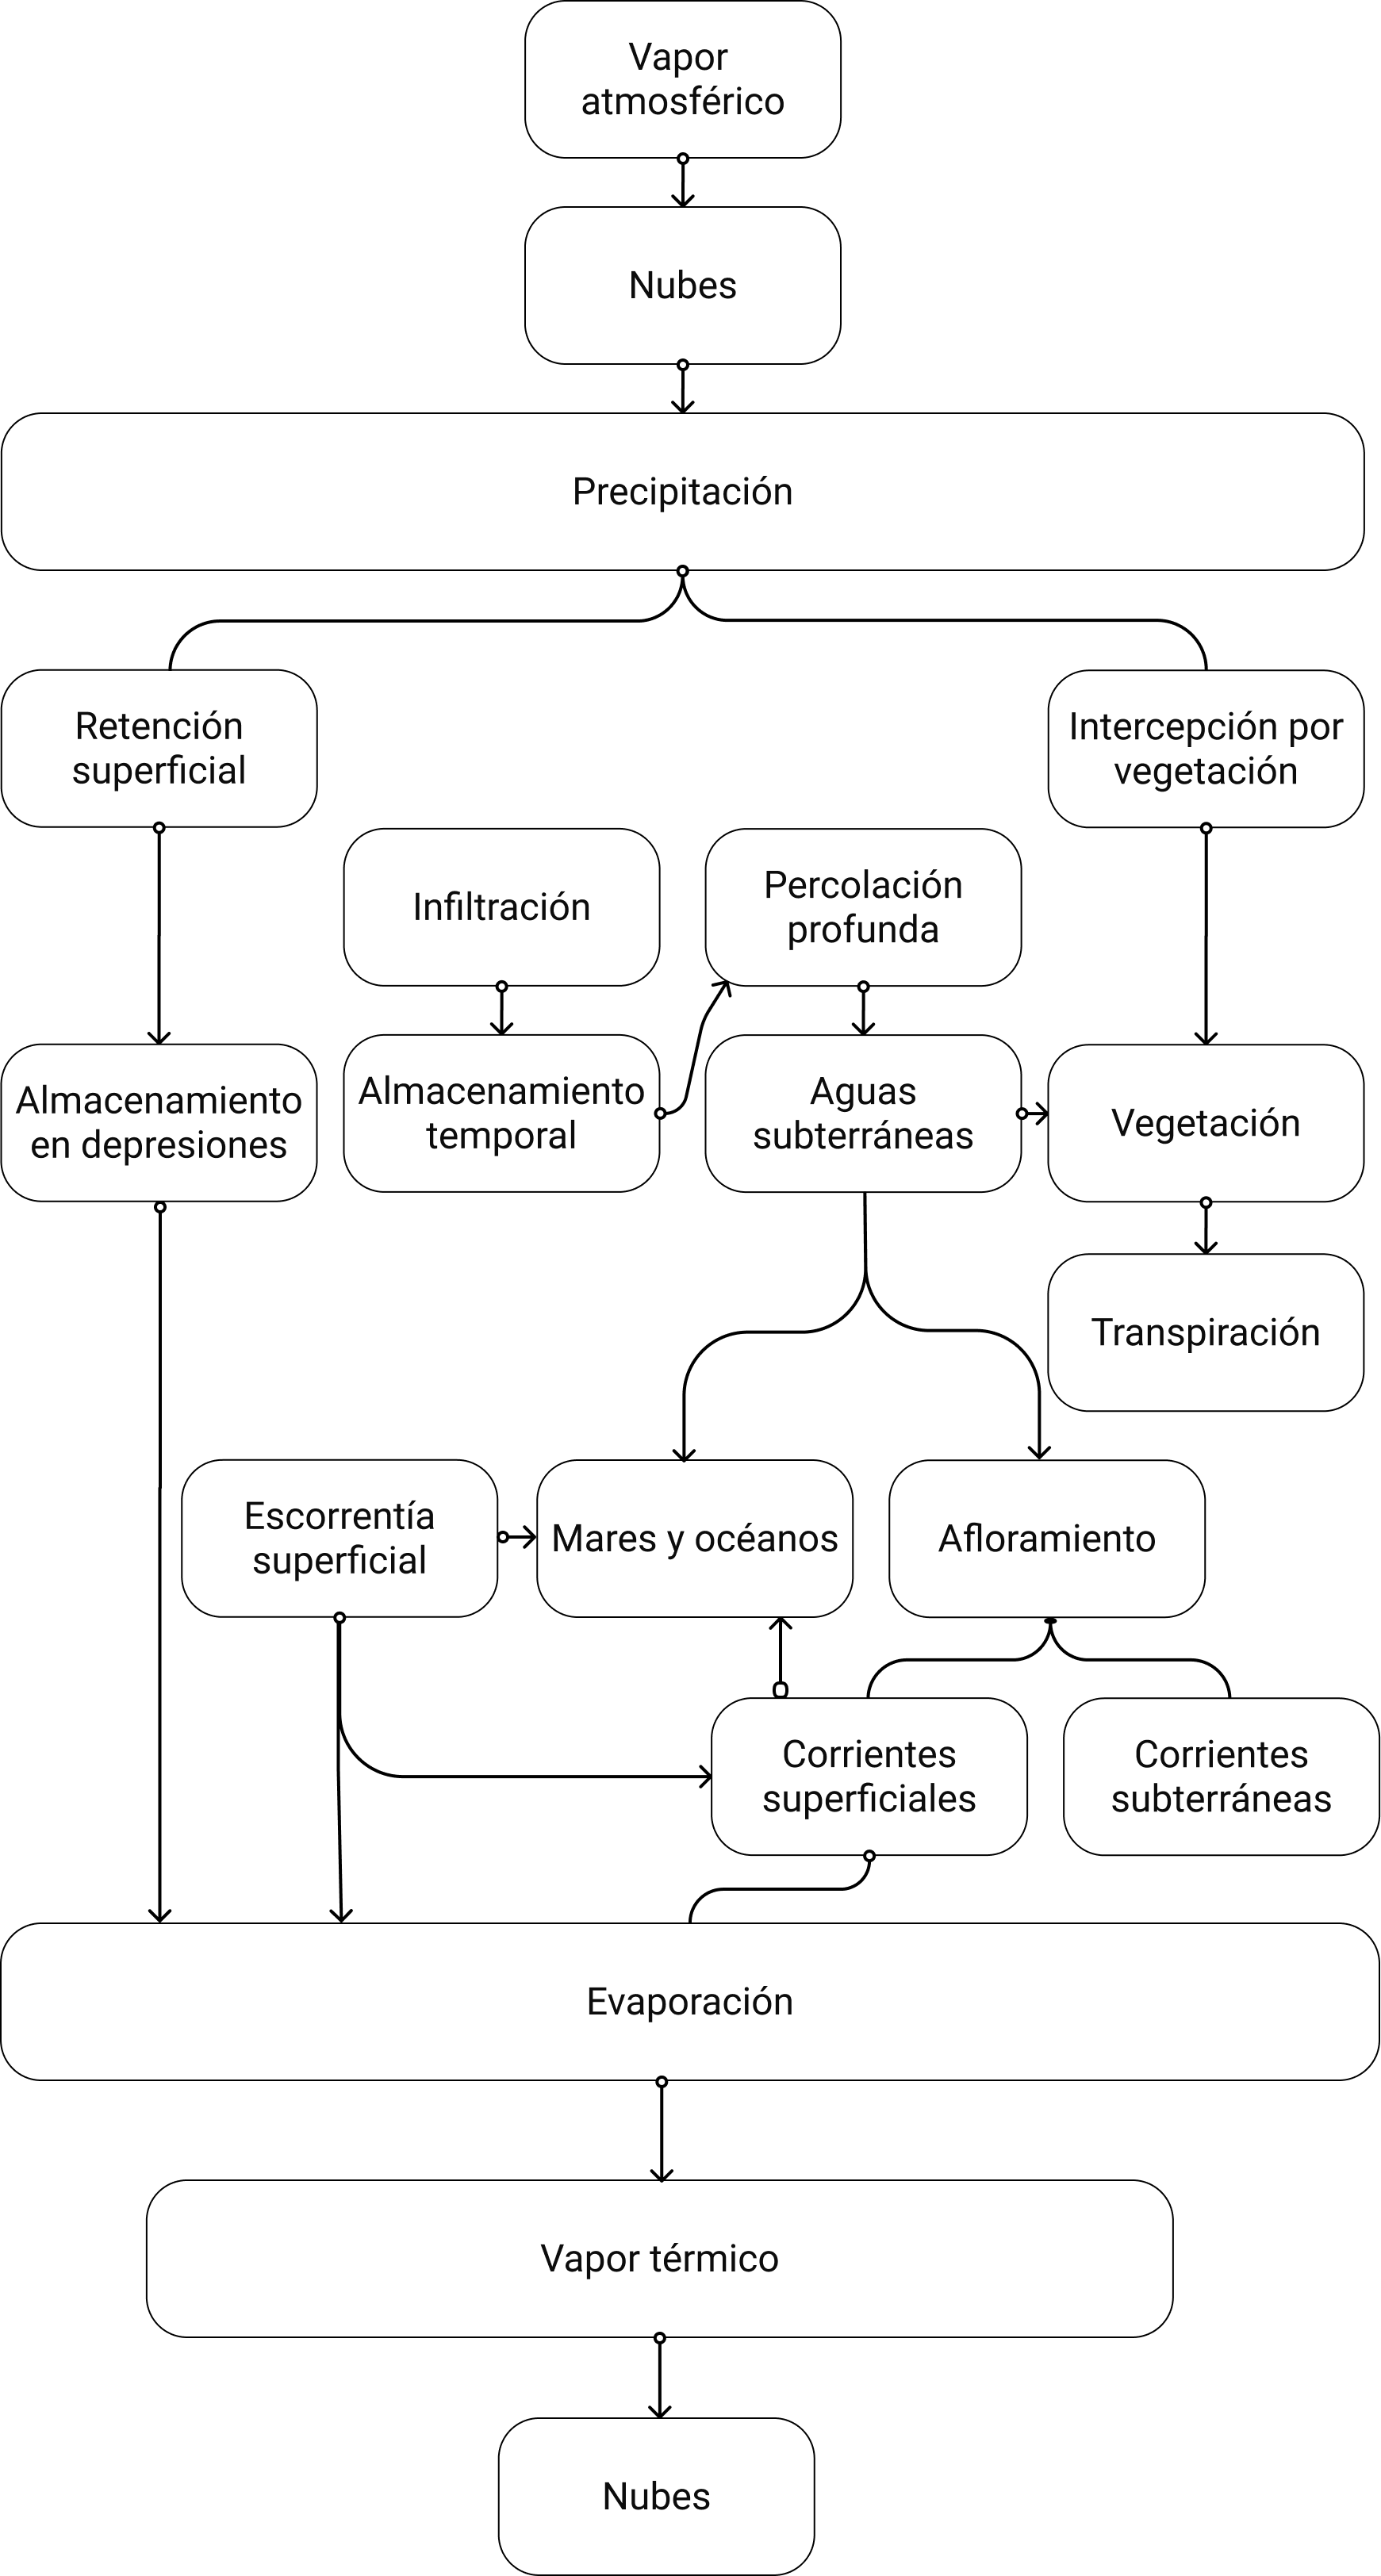
\includegraphics[width=0.7\textwidth]{fii1.png}}
	\caption{ciclo del agua}
	\label{fii1}
\end{figure}
Se puede observar que en ciclo hidrológico (véase la figura \ref{fii1}) intervienen procesos complejos de evaporación, precipitación, transpiración, infiltración, percolación, afloramiento, almacenamiento y escurrimiento. Para representar el ciclo hidrológico, se han hecho diferentes diagramas, algunos meramente descriptivos como el mostrado en la figura \ref{fii4}.
\subsubsection{Evaluación del Ciclo Hidrológico.} \label{subsubciclohidro}
A nivel mundial la energía solar evapora y eleva alrededor de: $500,000 Km^3$ de agua de la superficie terrestre, de la cual 86\% son de los océanos y 14\% de suelos. Una cantidad equivalente se precipita en la superficie en forma de lluvia, nieve o granizo: de la cual 78\% cae en la superficie de los océanos, lagos y lagunas; 22\% cae en la superficie terrestre, esto significa que el sistema transfiere $38,800 Km^3$ de \textbf{agua} de los océanos a continentes.

Para completar el Ciclo, el agua puede regresar a los océanos en forma
de escurrimiento.
\begin{figure}[h!]
	\centering
	\begin{subfigure}[b]{0.4\linewidth}
		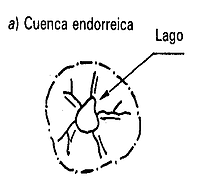
\includegraphics[width=\linewidth]{fii2.png}
		\caption{Una cuenca es una zona de la superficie terrestre en donde (si fuera impermeable) las gotas de lluvia que caen sobre ella tienden a ser drenadas por el sistema de corrientes hacia un mismo punto de salida.}
		\label{fii2}
	\end{subfigure}
	\begin{subfigure}[b]{0.4\linewidth}
		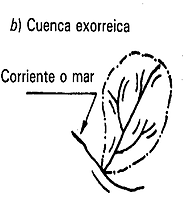
\includegraphics[width=\linewidth]{fii3.png}
		\caption{El punto de salida está dentro de los límites de la cuenca y generalmente es un lago.}
		\label{fii3}
	\end{subfigure}
	\caption{Su punto de salida está en los límites de las cuencas y está en
		otra corriente o mar.}
	\label{fig2-3}
\end{figure}
\begin{figure}[h!]
	\centerline{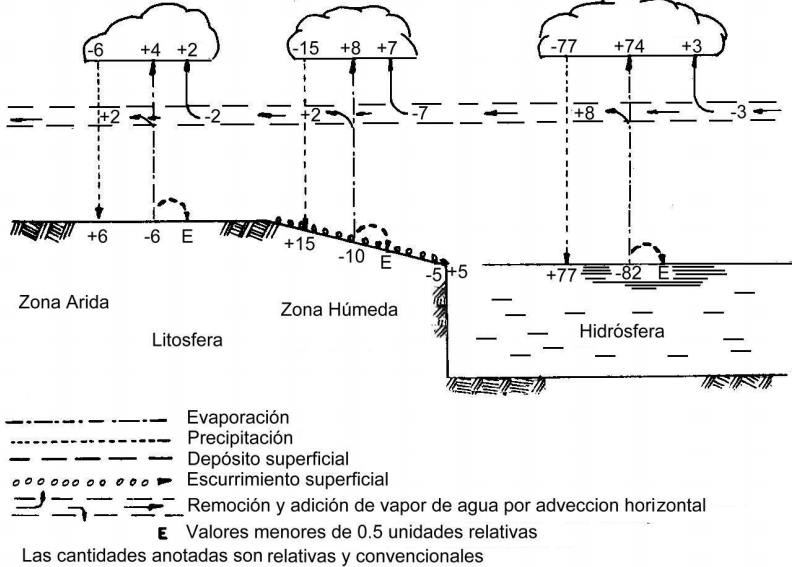
\includegraphics[width=0.7\textwidth]{fii4.png}}
	\caption{Representación cuantitativa del ciclo hidrológico.}
	\label{fii4}
\end{figure}
En México, la precipitación media anual es de 780 mm equivalente a $1,530 Km^3$, distribuida en forma genérica: $\frac{2}{3}$ partes en el sur y $\frac{1}{3}$ parte en el norte del país y concentrada en los meses de junio a octubre. De la anterior precipitación, el 68\% se evapotranspira, el 5\% se infiltra o percola recargando acuíferos, y el restante 27\% escurre superficialmente, representando un volumen de 410,000 millones de $m^3$, definido como \textbf{escurrimiento superficial virgen}, distribuido de la siguiente forma: en el 30\% de la superficie del país, en la zona norte, se genera tan solo el 4\% del escurrimiento, mientras que en el 20\% del territorio, en la zona sudeste y zonas costeras, se genera el 50\% del escurrimiento. Estas irregularidades espaciales y temporales plantean un reto especial en el manejo del agua de nuestro país.

Haciendo un balance del escurrimiento superficial, primeramente, a nivel regional, Los datos a nivel nacional están en la tabla \ref{tabone}
\begin{table}[h!]
	\centering
	\begin{tabular}{|c|c|c|c|c|c|c|}
		\hline
		\multicolumn{3}{|c|}{Disponibilidad Hídrica}                            & \multirow{3}{*}{\begin{tabular}[c]{@{}c@{}}Extracción\\ Para Usos\\ Consuntivos\end{tabular}} & \multirow{3}{*}{Exportac.(*)} & \multirow{3}{*}{Evaporación} & \multirow{3}{*}{Balance}                    \\ \cline{1-3}
		\multirow{2}{*}{\begin{tabular}[c]{@{}c@{}}Esc. \\ Virgen\end{tabular}} & \multirow{2}{*}{\begin{tabular}[c]{@{}c@{}}Retor.\\ Utiliz\end{tabular}}                      & \multirow{2}{*}{Import. (*)}  &                              &                          &          &       \\
		                                                                        &                                                                                               &                               &                              &                          &          &       \\ \hline
		410.7                                                                   & 2.98                                                                                          & 1.93                          & 49.2                         & 0.43                     & de Vasos & 357.6 \\ \hline
	\end{tabular}
	\caption{Balance del Agua Superficial en la República Mexicana (en $Km^3$/año) (*) Se importan de E.U. 1.85 $Km^3$ /año a la región noroeste y 0.07 a la región Norte y se exportan a E.U. 0.43 de la región Norte, comprometidos mediante el Acuerdo de carácter Internacional, así como 47.0 importados de Guatemala en la región sureste, sobre los cuales no existe convenio. El resto en importaciones y exportaciones son transferencias entre cuencas nacionales.}
	\label{tabone}
\end{table}
\subsection{Clasificación del Temporal}
Considerando la principal fase básica del ciclo hidrológico: la precipitación, y de
la cual dependen todas las \textbf{zonas de temporal}, en las que para producir alimentos,
se requiere de un temporal adecuado. Tomando solo en cuenta las condiciones medias anuales \autocite{Muñoz1976} de:
\begin{itemize}
	\item La precipitación pluvial
	\item y la temperatura
\end{itemize}
En un intento inicial el temporal ha sido clasificado, como en la tabla \ref{tabtwo} :
\begin{table}[h!]
	\centering\begin{tabular}{|l|l|l|l|}
		\hline
		\centering
		No & TIPO DE TEMPORAL & PRECIPITACIÓN          & TEMPERATURA                                                                                                                                                \\ \hline
		1  & EFICIENTE        & $> 700 mm$             & Entre 20 y 29$^{\circ}$C                                                                                                                                   \\ \hline
		2  & DEFICIENTE       & Entre $400$ y $700 mm$ & Entre 10 y 20$^{\circ}$C                                                                                                                                   \\ \hline
		3  & MALO             & $< 400 mm$             & \begin{tabular}[c]{@{}l@{}}Menor de 10 $^{\circ}$C y\\ Mayor de 29 $^{\circ}$C \end{tabular} \\ \hline
	\end{tabular}
	\caption{Clasificación del Temporal de acuerdo a la Precipitación y Temperatura.}
	\label{tabtwo}
\end{table}
\subsubsection{División del Territorio Nacional según su Precipitación}
En la república mexicana, las lluvias están irregularmente distribuidas durante los meses del año y en ocasiones hay localidades donde la precipitación de un mes cae en un solo día. Más del 65\% de la lluvia anual se presenta en solo cuatro meses, de junio a septiembre. Desafortunadamente, la ausencia de lluvias coincide frecuentemente con la máxima demanda de humedad por las plantas, lo que acentúa la condición de aridez de muchas regiones, independientemente de la reducida magnitud de la precipitación. Con excepción de Baja California y, en parte, de la costa de Sonora y Sinaloa, el régimen pluvial dominante se caracteriza por un periodo seco de noviembre a mayo y otros con lluvias de junio a octubre.

Además de ser el monto total de la lluvia, en general escaso durante el año y mal distribuido en los diversos meses, con frecuencia se presentan uno o varios años consecutivos de sequías.

Por lo que se refiere a las escasas lluvias invernales, estas provienen, en México, de masas de aire polar que descienden desde Canadá e invaden casi todo el país, causando algunas lluvias, frentes fríos y heladas. En el verano, al país llegan de ambos mares, vientos muy cargados de humedad que producen importantes lluvias, tanto en las cuencas de los ríos de la vertiente del Golfo como en la del Pacifico, y aún en la altiplanicie, lo que determina que las corrientes situadas, sobre todo en dichas vertientes, produzcan escurrimientos de consideración en esa época.

México recibe también la influencia de los ciclones tropicales, los cuales se forman durante el verano en los mares cálidos, próximos al Ecuador.

En la figura \ref{fii5} se muestra esquemáticamente cómo se distribuyen las lluvias en la república mexicana.
\begin{figure}[h!]
	\centerline{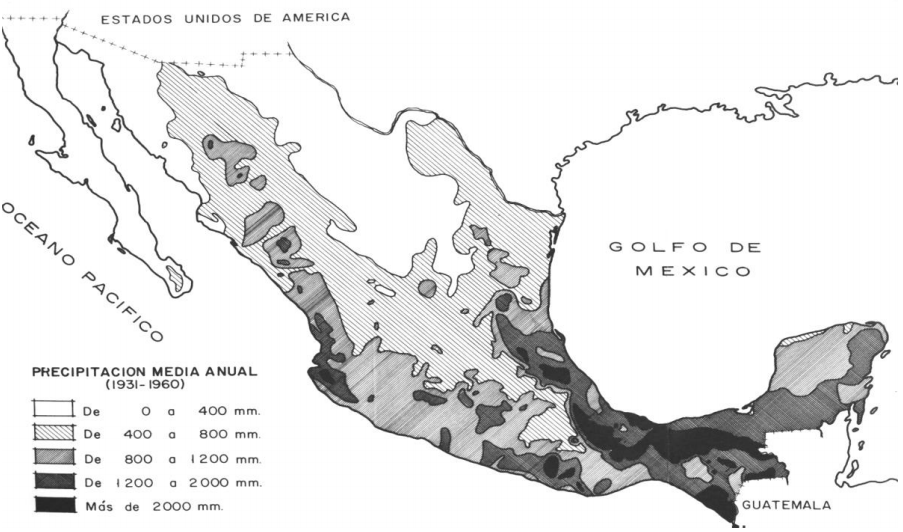
\includegraphics[width=1\textwidth]{fii5.png}}
	\caption{División del Territorio Nacional según la precipitación.}
	\label{fii5}
\end{figure}
\subsubsection{Formas de clasificación del Territorio nacional de acuerdo a la necesidad de Irrigación.}
De acuerdo al monto anual, distribución mensual de las lluvias, temperaturas y humedad atmosférica, el territorio nacional \autocite{Orive1970}, (según la necesidad de irrigación), se puede clasificar de acuerdo a la Tabla \ref{tabtree}:
\begin{table}[h!]
	\centering
	\begin{tabular}{|c|c|c|}
		\hline
		No  & Tipo de temporal   & Observaciones                                                                                                                                                                                                                        \\ \hline
		1   & Zona Húmeda        & No se requiere de la irrigación                                                                                                                                                                                                      \\ \hline
		2   & Zona Árida         & Sólo hay agricultura si aplicamos irrigación                                                                                                                                                                                         \\ \hline
		3   & Zonas Intermedias: & \begin{tabular}[c]{@{}c@{}}Las lluvias permiten el desarrollo\\ de cultivos sin necesidad de la irrigación.\end{tabular}                                                                                                             \\ \hline
		3.1 & Zona Semihúmeda    & \begin{tabular}[c]{@{}c@{}}Más del 50\% de los años, la lluvia es suficiente para\\ obtener una cosecha sin irrigación.\end{tabular}                                                                                                 \\ \hline
		3.2 & Zona semiárida     & \begin{tabular}[c]{@{}c@{}}Predominan los años con periodos de lluvias\\ insuficientes, se requiere el riego de auxilio\\ durante la temporada de lluvias, haciéndose\\ indispensable el riego en la temporada de secas\end{tabular} \\ \hline
	\end{tabular}
	\caption{Forma de clasificación del territorio Nacional según la necesidad de
		Irrigación.}
	\label{tabtree}
\end{table}
\subsubsection{Comparación de los estudios realizados sobre la necesidad de irrigación.}
Con posterioridad al estudio de 1944 de la Comisión Nacional de Irrigación (CNI), en 1958 la Secretaria de Recursos Hidráulicos hizo un nuevo estudio con mayor acopio de datos, acerca del panorama de México desde el punto de vista de la necesidad de irrigación. En 1961 la UNAM realizó otro estudio donde consideraba el índice de aridez de Emberger y por último en 1969 donde se racionalizaba el primer estudio subdividiendo las zonas extremas (Tabla \ref{tabfour}).
\begin{table}[h!]
	\centering
	\begin{tabular}{|c|c|c|c|c|c|c|c|}
		\hline
		\multicolumn{2}{|c|}{\begin{tabular}[c]{@{}c@{}}Estudio\\de 1944\end{tabular}} & \multicolumn{2}{c|}{\begin{tabular}[c]{@{}c@{}}Estudio\\de 1958\end{tabular}} & \multicolumn{2}{c|}{\begin{tabular}[c]{@{}c@{}}Estudio\\de 1961\end{tabular}} & \multicolumn{2}{c|}{\begin{tabular}[c]{@{}c@{}}Estudio de\\ 1969\end{tabular}}                                                                                    \\ \hline
		ZONA                                                                           & \%                                                                            & ZONA                                                                          & \%                                                                             & ZONA       & \%     & ZONA                                                  & \% \\ \hline
		Árida                                                                          & 52{.}1                                                                        & \begin{tabular}[c]{@{}c@{}}Riego\\ Indispensable\end{tabular}                 & 62{.}8                                                                         & Desértica  & 4{.}3  & \begin{tabular}[c]{@{}c@{}}Muy\\Árida \end{tabular}   & 23 \\ \hline
		\begin{tabular}[c]{@{}c@{}}Semi-\\árida\end{tabular}                           & 30{.}6                                                                        & \begin{tabular}[c]{@{}c@{}}Riego\\ Necesario\end{tabular}                     & 31{.}2                                                                         & Árida      & 33{.}9 & Árida                                                 & 20 \\ \hline
		\begin{tabular}[c]{@{}c@{}}Semi-\\humeda\end{tabular}                          & 10{.}5                                                                        & \begin{tabular}[c]{@{}c@{}}Riego \\ Conveniente\end{tabular}                  & 4{.}5                                                                          & semiárida  & 33{.}4 & semiárida                                             & 34 \\ \hline
		Húmeda                                                                         & 6{.}8                                                                         & \begin{tabular}[c]{@{}c@{}}Riego\\Inecesario\end{tabular}                     & 1{.}5                                                                          & Transición & 11{.}7 & \begin{tabular}[c]{@{}c@{}}Semi-\\humeda\end{tabular} & 16 \\ \hline
		\multicolumn{4}{|c|}{\multirow{3}{*}{}}                                        & \begin{tabular}[c]{@{}c@{}}Semi-\\húmeda\end{tabular}                         & 10{.}4                                                                        & Húmeda                                                                         & 4                                                                                \\ \cline{5-8}
		\multicolumn{4}{|c|}{}                                                         & Húmeda                                                                        & 4{.}8                                                                         & \begin{tabular}[c]{@{}c@{}}Muy\\húmeda\end{tabular}                            & 3                                                                                \\ \cline{5-8}
		\multicolumn{4}{|c|}{}                                                         & \begin{tabular}[c]{@{}c@{}}Muy\\Humeda\end{tabular}                           & 1{.}5                                                                         & \multicolumn{2}{c|}{}                                                                                                                                             \\ \hline
	\end{tabular}
	\caption{Comparación de estudios sobre la necesidad de irrigación en
		México }
	\label{tabfour}
\end{table}

%\begin{table}[h!]
%  \begin{tabular}{|c|c|c|c|c|c|c|c|}
%  \hline
%  \multicolumn{2}{|c|}{Estudio de 1944}  & \multicolumn{2}{c|}{Estudio de 1958}                                    & \multicolumn{2}{c|}{\begin{tabular}[c]{@{}c@{}}Estudio de\\ 1961\end{tabular}}   & \multicolumn{2}{c|}{Estudio de 1969} \\ \hline
%  ZONA                 & \%              & ZONA                                                           & \%     & ZONA                                      & \%                                   & ZONA                  & \%           \\ \hline
%  Árida                & 52{.}1          & Riego Indispensable                                            & 62{.}8 & Desértica                                 & 4{.}3                                & Muy Árida             & 23           \\ \hline
%  semiárida            & 30{.}6          & Riego Necesario                                                & 31{.}2 & Árida                                     & 33{.}9                               & Árida                 & 20           \\ \hline
%  Semihúmeda           & 10{.}5          & Riego Conveniente                                              & 4{.}5  & semiárida                                & 33{.}4                                & semiárida             & 34           \\ \hline
%  Húmeda               & 6{.}8           & \begin{tabular}[c]{@{}c@{}}No se necesita\\ Riego\end{tabular} & 1{.}5  & Transición                                & 11{.}7                               & Semihúmeda            & 16           \\ \hline
%  \multicolumn{4}{|c|}{\multirow{3}{*}{}}                                                                           & Semihúmeda                               & 10{.}4                               & Húmeda                & 4            \\ \cline{5-8} 
%  \multicolumn{4}{|c|}{}                                                                                            & Húmeda                                    & 4{.}8                               & MuyHúmeda             & 3            \\ \cline{5-8} 
%  \multicolumn{4}{|c|}{}                                                                                            & Muy Húmeda                                & 1{.}5                               & \multicolumn{2}{c|}{}                \\ \hline
%  \end{tabular}
%  \caption{Comparación de estudios sobre la necesidad de irrigación en
%  México }
%  \label{tabfour}
%\end{table}

Con los datos de lluvias, temperaturas, evaporaciones, etc$\dots$ Aportados por las estaciones climatológicas existentes en el país, así como los aportados por las nuevas estaciones que se instalen y los procedimientos tecnológicos que se desarrollen, será posible que se emprendan nuevos estudios, para los que Orive (1970) recomienda que se consideren las siguientes zonas, tomando las mismas dos zonas “límites”, o sea aquellas en que no puede haber agricultura si no hay riego, y aquellas en que no se necesita la irrigación para obtener una cosecha; para las zonas intermedias recomienda considerar a cinco, tal como se muestra en la Tabla \ref{tabfive}.
\begin{table}[h!]
	\centering
	\begin{tabular}{|c|c|}
		\hline
		ZONA & CARACTERÍSTICAS                                                                                                                                                                                                                                                                                                          \\ \hline
		I    & \begin{tabular}[c]{@{}c@{}}Donde el riego sea \\ absolutamente indispensable\end{tabular}                                                                                                                                                                                                                                \\ \hline
		II   & \begin{tabular}[c]{@{}c@{}}Donde del 0 al 20\% de los años \\ sea probable obtener una cosecha de\end{tabular}                                                                                                                                                                                                           \\ \hline
		III  & temporal (secano)                                                                                                                                                                                                                                                                                                        \\ \hline
		IV   & \begin{tabular}[c]{@{}c@{}}Donde la probabilidad sea \\ del 20\% al 40\% de los años\end{tabular}                                                                                                                                                                                                                        \\ \hline
		V    & Donde sea del 40\% al 60\%                                                                                                                                                                                                                                                                                               \\ \hline
		VI   & \begin{tabular}[c]{@{}c@{}}Donde la probabilidad \\ sea del 60\% al 80\%\end{tabular}                                                                                                                                                                                                                                    \\ \hline
		VII  & \begin{tabular}[c]{@{}c@{}}Donde sea del 80\% al 100\% Donde todos los años sea \\ probable obtener una cosecha\\ de temporal y por lo tanto el riego básicamente no se\\  necesite (pero en que muy\\ probablemente serán necesarias costosas obras \\ de desagüe y drenaje)\textbackslash{}end\{tabular\}\end{tabular} \\ \hline
	\end{tabular}
	\caption{Recomendación de zonas para futuros estudios sobre la necesidad de irrigación}
	\label{tabfive}
\end{table}

\subsubsection{Terrenos con posibilidades de aprovechamiento para el desarrollo agrícola de México.}
Se estima que las tierras llanas, o sea aquellas que tienen una pendiente menor del 10 \% tienen una superficie que, en números redondos, es del orden de unos 70 millones de hectáreas. Los terrenos con pendiente hasta de 25\% se han estimado en 140 millones de hectáreas. La distribución aproximada de las superficies anteriores para las cuatro zonas en que se ha dividido a México por su aridez, se muestra en la Tabla\ref{tabsix} :
\begin{table}[h!]
	\centering
	\begin{tabular}{|c|c|c|c|}
		\hline
		\multirow{2}{*}{ZONAS}                                                                                                                                                        & \begin{tabular}[c]{@{}c@{}}Con\\ Pendiente\\ de 0 a 10\%\\ Planas\end{tabular} & \begin{tabular}[c]{@{}c@{}}Con pendiente de\\ 10\% a 25\%\\ Obras de\\ Conservación de\\ Suelos\\ Fundamentales\end{tabular} & TOTAL \\ \cline{2-4}
		                                                                                                                                                                              & \multicolumn{3}{c|}{(en millones de ha)}                                                                                                                                                                              \\ \hline
		\begin{tabular}[c]{@{}c@{}}Áridas: Solo con riego puede\\ haber agricultura.\end{tabular}                                                                                     & 45                                                                             & 35.0                                                                                                                         & 80.0  \\ \hline
		\begin{tabular}[c]{@{}c@{}}semiáridas: Riego necesario\\ para eliminar lo aleatorio.\end{tabular}                                                                             & 12.5                                                                           & 17.5                                                                                                                         & 30.0  \\ \hline
		\begin{tabular}[c]{@{}c@{}}Semihúmedas: Temporal posible\\ en la mayoría de los años, pero\\ riego conveniente para eliminar\\ riesgos.\end{tabular}                          & 8.0                                                                            & 12.0                                                                                                                         & 20.0  \\ \hline
		\begin{tabular}[c]{@{}c@{}}Húmedas: Son indispensables\\ obras de drenaje y desagüe.\\ Riego de Auxilio en muchos casos\\ conveniente para cultivos\\ intensivos\end{tabular} & 4.5                                                                            & 5.5                                                                                                                          & 10.0  \\ \hline
		Sumas                                                                                                                                                                         & 70.0                                                                           & 70.0                                                                                                                         & 140.0 \\ \hline
	\end{tabular}
	\caption{Terrenos que serían aprovechables para el desarrollo agrícola de México}
	\label{tabsix}
\end{table}
Desde el punto de vista de la Irrigación, la superficie que es de interés es la de labor o laborable, la que se ha definido de acuerdo a los siguientes factores:
\begin{itemize}
	\item La limitación de los terrenos en lo correspondientes a pendientes no mayores del 10\%.
	\item La Escasez y mala distribución de las lluvias.
	\item Lo accidentado de su topografía.
	\item Lo erosionado de muchos suelos
	\item Su mal drenaje.
	\item La excesiva concentración salina de algunas tierras en las regiones áridas y semiáridas.
\end{itemize}
De acuerdo a estos factores se observa en la tabla \ref{tabseven}:
\begin{table}[h!]
	\centering
	\begin{tabular}{|l|l|l|}
		\hline
		\multirow{2}{*}{\textbf{Clasificación}}                 & \multicolumn{2}{l|}{\textbf{Superficie}}               \\ \cline{2-3}
		                                                        & \textbf{(en millones de ha)}             & \textbf{\%} \\ \hline
		De labor y laborable                                    & 29.3                                     & 14.9        \\ \hline
		Pastos en llanuras y lomeríos                           & 16.6                                     & 8.5         \\ \hline
		Pastos en terrenos cerril                               & 69.0                                     & 35.2        \\ \hline
		Superficie Forestal                                     &                                          & 33.7        \\ \hline
		Superficie inútil, no beneficiable para la agricultura. & 66.1                                     & 7.7         \\ \hline
		SUMAS:                                                  & 15.4                                     & 100.0       \\ \hline
	\end{tabular}
	\caption{Clasificación de la superficie del Territorio Nacional.}
	\label{tabseven}
\end{table}
Es necesario que se revisen las anteriores superficies tomando en cuenta la posibilidad de que, en un futuro no muy distante, se puedan llegar a eliminar, modificar o corregir algunos de los factores limitantes antes citados, gracias a una tecnología más avanzada y teniéndose en cuenta la presión que ejercerán las futuras e imperiosas necesidades de México, de que aumente su producción agrícola, no solo incrementando los rendimientos, sino también la superficie cultivable con buenas probabilidades de éxito.
\subsubsection{Superficie regable estimada en el territorio nacional.}
En un estudio realizado por la Secretaria de Recursos Hidráulicos en el año 1959, se hicieron las siguientes hipótesis para determinar el potencial agrícola con fines de riego en México, detalladas por Orive.
\begin{enumerate}
	\item Que el máximo aprovechamiento del agua superficial se logre construyendo presas de almacenamiento con las que se pueda llegar a utilizar el 75\% del volumen medio anual.
	\item Que se empleen los siguientes coeficientes de riego:
	      \begin{itemize}
		      \item Para climas desérticos y áridos: 12 000 $m^3/ha$
		      \item Para climas semi-áridos: 11,000 $m^3/ha$
		      \item Para climas semi-húmedos: 10,000 $m^3/ha$
		      \item Para climas húmedos: 9,000 $m^3/ha$
	      \end{itemize}
	\item Del agua aprovechada, ocurran retornos con valor del 20\% y que de estos retornos sea factible volver a aprovechar el 50\%.
\end{enumerate}
La superficie resultante se muestra en la Tabla \ref{tabeight}, se observa que el total de Área Neta Regable resulta de 11.45 millones de hectáreas la cual puede variar dependiendo de nuevos factores que puedan ser introducidos en el desarrollo del aprovechamiento del agua en México, que permiten prever que la superficie cultivable con agua segura puede ser mayor a la citada por Orive. Uno de estos estriba en la posibilidad de avanzar en la posibilidad de llevar aguas de cuencas donde existen más recursos hidráulicos que tierras que regar, a cuencas en que esta condición es la contraria, permitiría regar más superficie. En la tabla \ref{tabeight}, se consideró que con los retornos podía regarse una superficie de cerca de 800,000 hectáreas.
\begin{table}[h!]
	\centering
	\begin{tabular}{|c|c|c|c|c|c|}
		\hline
		\multirow{3}{*}{ZONA} & \multicolumn{2}{c|}{\begin{tabular}[c]{@{}c@{}}Agua superficial\\ media anual\end{tabular}} & \multirow{2}{*}{\begin{tabular}[c]{@{}c@{}}Área regable\\ hidrológicamente\end{tabular}} & \multirow{2}{*}{\begin{tabular}[c]{@{}c@{}}Área laborable\\ disponible\end{tabular}} & \multirow{2}{*}{\begin{tabular}[c]{@{}c@{}}Área neta\\ regable\end{tabular}}              \\ \cline{2-3}
		                      & Total                                                                                       & 75\%                                                                                     &                                                                                      &                                                                              &            \\ \cline{2-6}
		                      & \multicolumn{2}{c|}{Millones de $m^3$}                                                      & ha                                                                                       & ha                                                                                   & ha                                                                                        \\ \hline
		Desértica y árida     & 63,255                                                                                      & 47,441                                                                                   & 3,953,420                                                                            & 10,918,700                                                                   & 3,953,420  \\ \hline
		semiárida             & 49,363                                                                                      & 37,022                                                                                   & 3,365,640                                                                            & 7,139,700                                                                    & 3,365,640  \\ \hline
		Semihúmeda            & 5,811                                                                                       & 4,358                                                                                    & 435,800                                                                              & 1,511,000                                                                    & 435,800    \\ \hline
		Húmeda                & 238,848                                                                                     & 179,136                                                                                  & 19,909,000                                                                           & 3,696,500                                                                    & 3,696,500  \\ \hline
		TOTALES:              & 357,277                                                                                     & 267,927                                                                                  & 27,663,860                                                                           & 23,175,900                                                                   & 11,451,360 \\ \hline
	\end{tabular}
	\caption{Superficie regable estimada, según un estudio de 1959}
	\label{tabeight}
\end{table}
A través de varios años se han hecho diferentes consideraciones y estudios acerca de la potencialidad de México, en lo que corresponde a superficie factible y recursos hidrológicos disponibles \autocite{Cardenas1964}, para determinar el área máxima regable, los más importantes son los que se muestran en la Tabla \ref{tabnine}.
\begin{table}[h!]
	\centering
	\begin{turn}{90}
		\begin{tabular}{|c|c|c|c|c|c|c|}
			\hline
			\multirow{6}{*}{INVESTIGADOR}                                                     & \multirow{6}{*}{\begin{tabular}[c]{@{}c@{}}AÑO\\ DEL\\ ESTUDIO\end{tabular}} & \multicolumn{5}{c|}{S U P E R F I C I E S}                                                                                                                                                                                                                                                                                                                                       \\ \cline{3-7}
			                                                                                  &                                                                              & \multicolumn{2}{c|}{REGABLES}                                                   & \multirow{5}{*}{\begin{tabular}[c]{@{}c@{}}Riego\\ de\\ Auxilio\\ o \\ Humedad\end{tabular}} & \multirow{5}{*}{\begin{tabular}[c]{@{}c@{}}Riego\\ con\\ Aguas\\ de \\ Retorno\end{tabular}} & \multirow{2}{*}{\begin{tabular}[c]{@{}c@{}}TOTALES\\ en Ha\end{tabular}}                         \\ \cline{3-4}
			                                                                                  &                                                                              & \multirow{4}{*}{\begin{tabular}[c]{@{}c@{}}Aguas \\ superficiales\end{tabular}} & \multirow{4}{*}{\begin{tabular}[c]{@{}c@{}}Aguas\\ del\\ Subsuelo\end{tabular}}              &                                                                                              &                                                                          &                       \\ \cline{7-7}
			                                                                                  &                                                                              &                                                                                 &                                                                                              &                                                                                              &                                                                          &                       \\ \cline{7-7}
			                                                                                  &                                                                              &                                                                                 &                                                                                              &                                                                                              &                                                                          & \multicolumn{1}{l|}{} \\ \cline{7-7}
			                                                                                  &                                                                              &                                                                                 &                                                                                              &                                                                                              &                                                                          & \multicolumn{1}{l|}{} \\ \hline
			\begin{tabular}[c]{@{}c@{}}Adolfo Orive\end{tabular}                              & 1949                                                                         & 6 709 500                                                                       & 1 000 000                                                                                    & 2 291 500                                                                                    &                                                                          & 10 000 000            \\ \hline
			multirow{2}{*}{\begin{tabular}[c]{@{}c@{}}Rodríguez\\  Alba Antonio\end{tabular}} & 1957                                                                         & 10 000 000                                                                      & 2 700 000                                                                                    & 2 000 000                                                                                    &                                                                          & 14 700 000            \\ \hline
			Jorge L. Tamayo                                                                   & 1958                                                                         & 5 934 456                                                                       & 3 090 000                                                                                    & 2 000 000                                                                                    & 775 486                                                                  & 11 024 456            \\ \hline
			Andrés García Q.                                                                  & 1959                                                                         & 7 754 860                                                                       & 5 467 300                                                                                    & 3 696 500                                                                                    &                                                                          & 17 694 146            \\ \hline
			S.R.H.                                                                            & 1969                                                                         & 8 200 000                                                                       & 3 000 000                                                                                    &                                                                                              &                                                                          & 11 200 000            \\ \hline
		\end{tabular}
	\end{turn}
	\caption{Estudios realizados para la determinación de la Superficie Máxima
		Regable en México }
	\label{tabnine}
\end{table}
\subsection{Desarrollo de la Irrigación en diversas partes del mundo}

El origen de la agricultura bajo riego se pierde en la prehistoria más antigua. Algunos estudios muestran la utilización de la irrigación en Egipto hace 4,000 años, así como en China e igualmente en el Valle de Mesopotamia y en la India. En Egipto, en la actualidad las aguas del Nilo riegan aproximadamente 2,428,200 ha de tierras, que gran parte de estas son las mismas que se regaban antiguamente. Aquí existe la presa más antigua del mundo (hace 5,000 años) de 108 m de longitud y 12 m de altura.

En China, el riego lo utilizaban desde el año 2,627 años antes de Cristo (A.C.); en el siglo VII, D.C. se construyó un canal de 1,126 Km que fue usado primero en la navegación y después para el riego. Mucha superficie de tierra que en aquella época se regaba todavía da buenas cosechas en la actualidad. La presa Tu-Kiang actualmente sigue funcionando, fue construida por un hombre llamado Li y su hijo en los tiempos de la dinastía Chin (2,000 A.C.) y riega una extensión de más de 200,000 ha de arrozales.

En la región de Mesopotamia, en Asia Menor, los valles formados por los ríos Tigris y Eufrates, existen restos de antiguos de canales de riego, dos de ellos son los más largos de todos los tiempos, mostrando una gran habilidad en la irrigación de las civilizaciones antiguas.

En la India, existen presas en Ceylán (hoy Sri Lanka), que tienen más de 2,000 años. Testimonios de 300 años A.C. indican que el país se encontraba completamente regado y su prosperidad era muy grande a causa de las dos cosechas que podían colectar al año. En el sudoeste de Estados Unidos se evidencian restos de una civilización antigua basada en la agricultura de riego, trazos de antiguos canales son visibles todavía a lo largo del río Gila en Arizona.
\subsubsection{Distribución geográfica de la principal superficie de riego en el mundo.}
En el año 2012, la distribución geográfica de la principal superficie de riego en el mundo, de acuerdo a la FAO, tabla \ref{tabten}:
\begin{table}[h!]
	\centering
	\begin{tabular}{|c|c|c|}
		\hline
		No & PAÍS       & \begin{tabular}[c]{@{}c@{}}SUPERFICIE\\ (Millones de ha)\end{tabular} \\ \hline
		1  & INDIA      & 67                                                                    \\ \hline
		2  & CHINA      & 65                                                                    \\ \hline
		3  & USA        & 26                                                                    \\ \hline
		4  & PAKISTÁN   & 20                                                                    \\ \hline
		5  & IRÁN       & 8.4                                                                   \\ \hline
		6  & INDONESIA  & 7.5                                                                   \\ \hline
		7  & MÉXICO     & 6.5                                                                   \\ \hline
		8  & TAILANDIA  & 6.4                                                                   \\ \hline
		9  & BANGLADESH & 5.1                                                                   \\ \hline
		10 & TURQUÍA    & 5.0                                                                   \\ \hline
		11 & BRASIL     & 4.7                                                                   \\ \hline
		12 & VIETNAM    & 4.6                                                                   \\ \hline
		13 & RUSIA      & 4.3                                                                   \\ \hline
		14 & UZBEKISTÁN & 4.3                                                                   \\ \hline
		15 & EGIPTO     & 3.7                                                                   \\ \hline
		16 & IRAK       & 3.6                                                                   \\ \hline
		17 & ESPAÑA     & 3.4                                                                   \\ \hline
	\end{tabular}
	\caption{ Distribución geográfica de la principal superficie de riego en el mundo,
		al año 2012.}
	\label{tabten}
\end{table}
\subsubsection{Historia de la Irrigación en México}

\subsubsection*{La Irrigación Primitiva en México.}
Los Mexica se asentaron en el Valle de México cuando las enormes lagunas de Texcoco, Xochimilco, Chalco, Zumpango, etc$\dots$ ocupaban la mayor parte del valle. Estos lagos crecían y se desbordaban, por lo cual, para poder aprovechar sus aguas en usos urbanos, domésticos, así como para el riego, tuvieron que emprender una serie de acciones utilizando diques, canales, acueductos, presas, etc

Dentro de las anteriores acciones se encuentran también la llamada \textbf{``Chinampa''}, que es un campo de cultivo, jardín y habitación a la vez, aquí se llevan las tierras a las aguas. Estas están construidas con varas tejidas con raíces de plantas acuáticas y de otros materias ligeros, capaces de sostener unida la tierra de la Chinampa; sobre esta base se colocan ramas de las mismas plantas y encima el fango que sacan del fondo del lago, formando cuadriláteros de dimensiones variables.

Los trabajos de irrigación pre cortesanos, se deben a Netzahualcoyotl, estadista, poeta, filósofo y gran ingeniero que fue constructor del célebre vergel de Tezcutzingo y el dique o albarradón para dividir el lago de Texcoco (aguas saladas) del de México (aguas dulces), además de protegerlo contra las crecidas del mismo, evitando inundaciones.

El agua la conducían hacia los terrenos del regadío, desde lugares lejanos a través de acueductos llamados \textbf{``Apipilolli''} o por canales o acequias llamadas ``Apantli'', formando extensos sistemas de irrigación comunes a varios pueblos. En lugares propicios formaban grandes depósitos de agua de lluvias o albercas llamadas ``Tlaquilacaxitli'' a los que los españoles denominaron \textbf{``JAGÜEYES''}. En Cholula se encontraron restos de un acueducto de barro cocido de una sola pieza, con paredes de 30 cm de grueso, de sección toscamente circular con diámetro cercano a los 2m.
\subsubsection{Periodo Colonial}
La obra de colonización española estuvo encaminada a que las ciudades estuvieran abastecidas de agua, así como bien regados sus campos. Se hicieron vasos, acueductos, lagos artificiales, desviaciones de ríos y aprovechamientos de manantiales. En estas acciones se destacaron los frailes agustinos.

Los acueductos construidos durante esta época se cuentan por cientos; construidos con el objeto de regar los campos, huertos y para el abastecimiento de agua a poblaciones; entre estos se destacan: el de Epazoyucan de 15 Km de longitud, el de Tepeapulco de 23 Km, el acueducto de Guadalupe (12 Km y sustentado en 2310 arcos), los de Oaxaca, Morelia, Querétaro, Taxco, Chiapa de Corso, Atlacomulco, etc$\ldots$ En este periodo también se destacó la construcción de la Laguna de Yuriria por Fray Diego de Chávez, la cual es un hermoso lago artificial de 16 Km de largo por 6 Km de ancho.
\subsubsection{Periodo Independiente y Prerrevolucionario.}
En el último tercio del periodo se emprendieron algunas acciones como la construcción de algunas obras: La desecación de la Ciénaga de Chapala y los primeros canales de riego del Valle de Mexicali; obra de irrigación de Lombardía y Nueva Italia y diversos canales en la Comarca Lagunera.

Según lo detalla Orive, el único esfuerzo que se hizo por parte del gobierno de Porfirio Díaz para impulsar la construcción de obras de irrigación fue la creación en 1908 de “La Caja de Préstamos para Obra de Irrigación y Fomento de la Agricultura” con fundamento en la Ley del 17 de julio de 1908 facultando al ejecutivo para disponer de 25 millones de pesos del Tesoro Público con este fin.

Esta caja de Préstamos operó como Sociedad Anónima con un capital de 10 millones de pesos; emitió bonos con garantía del Gobierno federal por valor de 50 millones de pesos los que fueron colocados en el extranjero, e inició sus operaciones con más de 20 millones de pesos. Facilitaba fondos a grandes hacendados y a varias empresas agrícolas, ganaderas y hasta mineras, con garantía hipotecaria, interés de 7\% anual y plazo máximo de pago de 15 años. Los resultados de lo anterior fue que la mayoría de los deudores no cumplieron sus contratos y cuando las obras se ejecutaron, quedaron en manos de unos cuantos terratenientes que las explotaron en su beneficio personal.

\subsubsection{Periodo Posrevolucionario (Riego Institucional).}
En el periodo del año 1910 a 1915 se dio la etapa álgida de la lucha militar. Para 1915 en la ley del 6 de enero, se da la primera Ley Agraria, en la que se establecían una serie de derechos agrarios. Durante 1916, en la etapa final de construcción de la Presa Necaxa se presenta una falla en la cortina. En 1917, se presenta la Nueva Constitución Mexicana del 5 de febrero, mostrando en el artículo 27 su condición agraria, así como se presenta la terminación de la presa Boquilla (cortina de concreto y mampostería de 74 m de altura y 3,000 $Hkm^3$).

Para 1921, se crea la Dirección de Irrigación en la Secretaría de Agricultura y Fomento; esta Dirección se abocó a las siguientes acciones: a) Organización del Servicio Hidrológico, b) Estudio general de grandes proyectos (Yuriria y Tepuxtepec en el Lerma, el río Santiago en Aguascalientes, el Valle de Juárez en Chihuahua), c) Operación de obras de riego: Ciénaga de Chapala, Valle de Juárez y Canales del Yaqui. d) Construcción: reparación de canales Diaz, Marcos Carrillo y Vícam en el Valle del Yaqui, Reparación de diques y drenajes de la Ciénaga de Chapala y construcción de la presa Mexquitic en San Luis Potosí. En 1924 se crea la especialidad de Irrigación en la Escuela Nacional de Agricultura en San Jacinto, Distrito federal; así mismo se crea el departamento de Reglamentación e Irrigación, en sustitución de la dirección de Irrigación, con funciones notablemente reducidas y con raquítico presupuesto, funcionando así hasta 1925.

Para 1926 surge la Ley de Irrigación, reglamentando el uso de las aguas de propiedad Federal y se crea un nuevo organismo gubernamental: la Comisión Nacional de Irrigación (CNI). Esta comisión se enfrentó a dos grandes obstáculos por vencer: a) escasez de datos hidrométricos de las corrientes por aprovechar y b) la falta de personal especializado en el proyecto y construcción de las obras de irrigación. El primer obstáculo se decidió enfrentarlo construyendo dos obras: presa “Calles” y la Presa “Don Martín”, la primera con capacidad excesiva en su vaso y la segunda con una superficie proyecto de riego en forma excesiva. El segundo obstáculo, el gobierno resolvió no tratar de improvisar, sino traer a México un grupo brillante de ingenieros extranjeros, especializados en Irrigación, para lo cual la CNI estableció un contrato con empresas extranjeras para que estas, contando con los servicios de ingenieros verdaderamente especializados en el proyecto y la construcción de obras de riego, se encargarán de esos trabajos.

En el periodo de los años 1926 a 1928, se desarrolló la siguiente obra deirrigación: Presa Calles y la Presa Don Martín, así como la adaptación y reparación deobras construidas en el Distrito de Riego de Palestina, Coahuila para el riego de 1,600ha. Se adaptaron y ampliaron las obras de riego de Tula, para el riego de 33,800 ha. Seconstruyó la presa de Metztitlán, Hidalgo para el riego de 3,500 ha y se construyó laPresa Derivadora de Mante, Tamaulipas para regar 8,500 ha.
 
Para el periodo de los años 1929 a 1934, se construyó la siguiente obra de irrigación: Presa Abelardo Rodríguez en Baja California; obras de riego del Nogal, en Coahuila, que son aguas del río Sabinas, tributario del Salado, afluente del río Bravo; obras en Delicias, Chihuahua: Presa derivadora y canales; obras en Cd. Juárez: reacondicionamiento de canales y construcción de una red de drenes. En este periodo se pusieron bajo riego 146,600 ha.

En el periodo de los años de 1935 a 1940, se inició la construcción de grandes presas para irrigación: Presa El Palmito, en Durango, para el riego de 83,000 ha se inició en 1936 y se concluyó en 1946; la Presa Solis, en Guanajuato, para el riego de 102,500 ha se inició en 1939 y se concluyó en 1949; Presa Sanalona, en Sinaloa, para el riego de 94,000 ha se inició en 1939 y se concluyó en 1948; la Presa La Angostura, en Sonora, para el riego de 115,000 ha, se inició en 1936 y se concluyó en 1942 y la Presa Marte R. Gómez (El Azúcar) en Tamaulipas, para el riego de 66,000 ha, se inició en 1936 y concluyó en 1946.

Además se iniciaron las siguientes obras importantes: en Baja California, el mejoramiento de canales y drenes en el río Colorado; en Guerrero, una derivadora en el Río Cutzamala; en Hidalgo, la Presa Huichapan y canales en Ixmiquilpan; en Jalisco y Michoacán, obras de reforzamiento de diques y mejoramiento de drenes en la Ciénaga de Chapala; en Michoacán, la Presa Cointzio, canales y drenes en Morelia y Queréndaro, así como en Apatzingán; así como canales en diversos estados. La superficie puesta bajo riego (nueva y mejorada) en el periodo fue de 118,495 ha.

En este periodo se inicia la construcción de obras de pequeña irrigación (1937), para desarrollar infraestructura de riego en la altiplanicie mexicana. Para el periodo de los años de 1941 a 1946, como obra de irrigación se desarrolló la construcción de la Presa Abelardo Rodríguez en Sonora, y se continuó y concluyó buena parte de las iniciadas en el anterior periodo. En cuanto a la Pequeña Irrigación, la CNI construyó 66 obras con las que se puso bajo riego a 37,000 ha. En diciembre de 1946 se funda la Secretaria de Recursos Hidráulicos en sustitución de la CNI. La superficie puesta bajo riego (nueva y mejorada) en el periodo fue de 549,129 ha.

Durante el periodo de los años de 1947 a 1952, se construyeron las siguientes grandes presas: Álvaro Obregón en Sonora, para riego de 220,000 ha; Endo, en el río Tula en Hidalgo, para el riego de 5,000 ha; Mocúzari, en Sonora, para riego de 60,000 ha. En este periodo la obra de pequeña irrigación fue muy importante incorporando al riego 146,442 ha, de las 652,512 ha de riego nuevas y mejoradas para el periodo.

En 1947, se creó la Comisión del Papaloapan con el objeto de planear, diseñar y construir las obras requeridas para el desarrollo integral y armónico de la cuenca del río Papaloapan. Así mismo en el mismo año se creó la Comisión del Tepalcatepec, con idénticas finalidades, para 1960 se transforma en la Comisión del Balsas. Para el año de 1952, se funda la Comisión del Río Fuerte, iniciándose la construcción de la Presa Miguel Hidalgo; igualmente en el mismo año se crea la Comisión del Río Grijalva.

En el periodo de los años 1953 al 1958, la principal obra de grande irrigación consistió en la construcción de: la Presa El Marqués, en Oaxaca; La Presa Falcón, en Tamaulipas. La obra de Pequeña Irrigación incorporó al riego 148,000 ha. La superficie beneficiada fue de 748,000 ha para el periodo, con obras nuevas y mejoradas. En 1958 se crea la Comisión de Estudios del Río Pánuco.

Para el periodo comprendido entre los años 1959 a 1964, la obra de irrigación realizada consistió en la Presa La Amistad en Coahuila y la Presa Humaya (López Mateos), en Sinaloa, para riego de 90,000 ha; en la obra de pequeña irrigación se incorporó una superficie de 110,000 ha haciendo un total de superficie beneficiada de 251,000 ha para el periodo, con obras nuevas y mejoradas. En 1960 se crea la Comisión de Estudios del Río Lerma. Durante el periodo de los años 1965 al 1970, se crearon los siguientes organismos:
\begin{enumerate}
	\item El \textbf{PLHINO} (Plan HIdráulico del Noroeste) que perseguía el aprovechamiento conjunto de 17 ríos con 25,000 millones de $m^3$ anuales, tratando de que la superficie de riego existente de 874,000 ha se incrementará en 426,000 ha haciendo un total de 1’300,000 ha.
	\item El \textbf{PLHICEN} (Plan HIdráulico del Centro), creado para solucionar el problema de abastecimiento de agua a la zona metropolitana de la Ciudad de México y subsecuente uso de las aguas residuales en el riego.
	\item \textbf{PLHIGON} (Plan HIdráulico del Golfo Norte), que perseguía el permitir el aprovechamiento conjunto de las aguas de cuatro importantes cuencas del Noreste de la República Mexicana: Pánuco, Purificación, San Fernando y Bravo, conduciendo agua del Pánuco hacia Matamoros.
	\item \textbf{PNPI} (Plan Nacional de Pequeña Irrigación) con el objeto de dotar de riego en 10 años a 306,000 ha.
	\item  Plan de mejoramiento de la eficiencia en el uso del agua, con el objeto de aumentar la eficiencia de conducción del 50\% al 65\% en promedio y la Parcelaria del 50\% al 70\% haciendo un total de 45\%, a este último se le denominó \textbf{PLAMEPA} (Plan de Mejoramiento Parcelario), tratando de mejorar el uso del agua en la parcela.
\end{enumerate}
En el año de 1972 se decreta la Ley Federal de Aguas; en 1975 se crea la \textbf{CPNH} (Comisión del Plan Nacional Hidráulico), que intentaba establecer un plan maestro para detectar zonas críticas carentes de agua, identificándose las siguientes:
\begin{itemize}
	\item Área Crítica No 1. Zona metropolitana de la Ciudad de México
	\item Área Crítica No 2. Cuenca Alta y Media del Río Lerma en lo referente a la Contaminación de las aguas.
	\item Área Crítica No 3. Zona metropolitana de la Ciudad de Monterrey.
\end{itemize}
Para el año 1977 se decreta la desaparición de la Secretarías de Agricultura y Ganadería y la de Recursos Hidráulicos, creándose una nueva dependencia de gobierno: la Secretaría de Agricultura y Recursos Hidráulicos (\textbf{SARH}). En este año desaparecen todas la Comisiones, exceptuando a la CPNH y la Comisión del Ex-lago de Texcoco, así mismo se funda la Dirección General de Distritos de Temporal.

En 1986 se crea el Instituto Mexicano de Tecnología del Agua (\textbf{IMTA}), en sustitución de la CPNH. Para 1989 se funda la Comisión Nacional del Agua (\textbf{CNA}) a partir de la Subsecretaria de Infraestructura Hidráulica de la SARH, iniciándose el proceso de privatización de los distritos de riego, entregando la operación de la infraestructura de riego a nivel de red menor a Asociaciones de Usuarios, y constituyéndose como autoridad federal única en la materia. En el año de 1992 se promulga la Ley de Aguas Nacionales, destacándose entre sus objetivos: a) La administración integral del agua, con una mayor participación de los usuarios y entidades federativas a través de los consejos de cuenca; b) El aprovechamiento eficiente y racional del agua para la modernización del agua para la modernización del campo y en general para la modernización del país; c) La mayor participación de particulares en la construcción y operación de la infraestructura y servicios hidráulicos; d)La seguridad jurídica en el uso y aprovechamiento del agua, que permita a los particulares planear adecuadamente sus actividades a mediano y largo plazos; entre otros. Durante el año 1993 se decretan reformas sustanciales al Artículo 27 Constitucional permitiendo entre otras acciones el arrendamiento y venta de terrenos ejidales, así como el otorgamiento de concesiones a particulares para el aprovechamiento y manejo de los recursos hidráulicos. En 1994 la CNA se integra a la secretaria del Medio Ambiente Recursos Naturales y Pesca (\textbf{SEMARNAP}) como órgano desconcentrado de esta, y como organismo ejecutor de la política hidráulica en México se crea en su interior, en el año de 1996 el Programa de Modernización del Manejo del Agua (\textbf{Promma}), como instancia para ejecutar el programa hidráulico 1995-2000.

\subsection{Problemática y retos de la Irrigación en México.}
Los grandes problemas que se presentan en la actualidad, respecto a la Irrigación en México, es por un lado la insuficiencia de infraestructura para dar atención a la gran demanda de alimentos ante el crecimiento poblacional, que hace que se esté importando buena parte de los granos básicos fundamentales para alimentación del pueblo, tal es el caso del Maíz, que se importa el 55\% del consumo nacional, así mismo con el frijol, trigo, arroz, etc$\ldots$ Por otro lado, es la sobre explotación de las fuentes de aguas superficiales y subterráneas, en las primeras simplemente se agota el recurso y mucha superficie con infraestructura de riego que deja de usarse, por ejemplo de una superficie de los distritos de riego de 3.5 millones de hectáreas solamente se riegan 2.2 millones de hectáreas. En lo que corresponde a la sobreexplotación de las aguas subterráneas, es el abatimiento de los niveles de los acuíferos que derivan a severos problemas de calidad, tal situación sucede en los acuíferos costeros que se presentan problemas de intrusión salina, que nulifican la utilización de los mismos; y en los acuíferos continentales la aparición de aguas fósiles, con severos problemas de la presencia de arsénico en el agua y otros metales pesados, que sin ser detectables a primera vista genera severos problemas de salud en las personas usuarias del agua de esos acuíferos$\ldots$

Así mismo, es la gran contaminación que generan lo grandes centros de población, en el uso del agua que deriva a severos problemas de calidad con residuales cada vez más agresivos y que al no recibir ningún tratamiento, y utilizarse en el riego deriva a grandes problemas de calidad en los productos agrícolas y más en el caso de aquellos que se consumen crudos, y es la causa y origen de severos problemas de salud en las personas.
\subsubsection{Patrimonio Hidráulico de México acreditado para el año 1998}
\begin{itemize}
	\item 4,500 presas de almacenamiento (Grandes, Medianas y Pequeñas)
	\item 2,597 presas derivadoras
	\item 54,000 millones de $m^3$ de capacidad útil para riego
	\item 80,000 millones de $m^3$ de almacenamiento total.
	\item 80,775 Km de canales
	\item 29,450 Km de drenes y desagües
	\item 60,826 Km de caminos de operación y enlace de zonas agrícolas.
	\item 3,350 plantas de bombeo
	\item 150,000 pozos profundos
	\item 210,000 estructuras en canales, drenes y caminos todo lo anterior para regar 6.2 millones de ha, con lo cual México ocupa el 8º. Lugar mundial por su infraestructura de riego.
	\item 2,700 Km de acueductos que entregan 2,840 millones de$ m^3$ al año de agua en bloque a poblaciones.
	\item 76.5 millones de habitantes (83.5\%) con agua potable.
	\item 61.4 millones de habitantes (67.0\%) con servicio de alcantarillado.
	\item 818 plantas de tratamiento de aguas residuales de origen municipal.
	\item 43,000 l/s de capacidad instalada total (24.7\% del caudal total de aguas residuales de origen municipal).
	\item 5,300 l/s de tratamiento de aguas residuales de origen industrial (8.3\% del caudal total de aguas residuales de origen industrial).
	\item Más de 100 plantas hidroeléctricas
	\item 8,171 MW de capacidad instalada total
	\item 21\% de la energía total generada.
\end{itemize}
\subsubsection{Superficie puesta bajo riego para diferentes años, en México.}

Hasta el año de 1910 la superficie que se encontraba bajo riego era de
aproximadamente de 700,000 ha, una vez que el estado toma bajo su responsabilidad a
través de la Comisión Nacional de Irrigación en 1926 y lo hecho hasta 1930 se
estimaba que la superficie de riego era de 1,000,000 ha; de 1926 a 1966 la CNI hasta
1946 y de aquí la Secretaría de Recursos Hidráulicos pusieron bajo riego 2,543,302 ha
haciendo un total de 3,543,302 ha para 1966, estudios posteriores mostraban como se
dio la superficie bajo riego en 1976, 1979 y 1985, tal como se muestra en la Tabla \ref{tab11}.

\begin{table}[h!]
	\centering
	\begin{tabular}{|c|c|c|c|}
		\hline
		\multirow{2}{*}{}                                                                                                                                                                                                         & \multicolumn{3}{c|}{SUPERFICIES EN ha}                                                                                                                                                                                    \\ \cline{2-4}
		                                                                                                                                                                                                                          & \begin{tabular}[c]{@{}c@{}}Al 29 de marzo\\ de 1976\end{tabular}      & \begin{tabular}[c]{@{}c@{}}Al 20 de marzo\\ de 1979\end{tabular}        & A Dic. de 1985                                                          \\ \hline
		\begin{tabular}[c]{@{}c@{}}Operadas y supervisadas como \\ distritos de riego\\ \\ Operadas y supervisadas como\\ Unidades de Riego para el\\ Desarrollo Rural\end{tabular}                                               & \begin{tabular}[c]{@{}c@{}}2,846,970\\ \\ \\ \\  803,000\end{tabular} & \begin{tabular}[c]{@{}c@{}}3,000,000\\ \\ \\ \\  1,223,000\end{tabular} & \begin{tabular}[c]{@{}c@{}}3,215,000\\ \\ \\ \\  1,554,000\end{tabular} \\ \hline
		TOTAL SARH:                                                                                                                                                                                                               & 3,649,970                                                             & 4,223,000                                                               & 4,769,000                                                               \\ \hline
		\begin{tabular}[c]{@{}c@{}}Operadas por particulares y\\ otras dependencias de Gobierno\\ (incluyendo 430,000 ha\\ operadas y supervisadas con\\ bombeo de agua del subsuelo)\\ \\ Operadas por particulares\end{tabular} & \begin{tabular}[c]{@{}c@{}}1,214,456\\ \\  --\end{tabular}            & \begin{tabular}[c]{@{}c@{}}--\\ \\  777,000\end{tabular}                & \begin{tabular}[c]{@{}c@{}}--\\ \\  8000,00\end{tabular}                \\ \hline
		\begin{tabular}[c]{@{}c@{}}Total de Superficie Puesta Bajo\\ Riego:\end{tabular}                                                                                                                                          & 4,864,426                                                             & 5,000,000                                                               & 5,569,000                                                               \\ \hline
	\end{tabular}
	\caption{Obra de Irrigación y superficie puesta bajo riego por Instituciones
		Gubernamentales y por Particulares.}
	\label{tab11}
\end{table}
Posteriormente se han dado cifras aisladas
mencionando que para fines de los años ochenta la superficie ya era de 6,000,000 ha y
así se mantuvo hasta que recientemente en 1998, se mencionó que la superficie total
era de 6.2 millones de hectáreas (según el Programa Hidráulico 1995-2000, CNA \autocite{federal1996programa}), otras
fuentes señalan a 6.3 millones de hectáreas, distribuida de acuerdo al Programa
Hidráulico 1995-2000 en: 3.3 millones de hectáreas ubicadas en 80 distritos de riego y
2.9 millones de hectáreas radicada en más de 39,600 unidades de mediano y pequeño
riego.

\subsubsection{Costos de una hectárea nueva bajo riego}

\begin{table}[h!]
	\centering
	\begin{tabular}{|c|c|}
		\hline
		Año  & Costo (*)/ha  \\ \hline
		1970 & \$ 10,500     \\ \hline
		1976 & \$ 56,000     \\ \hline
		1980 & \$ 70,000     \\ \hline
		1985 & \$ 1,200,000  \\ \hline
		1987 & \$ 2,300,000  \\ \hline
		1990 & \$ 7,500,000  \\ \hline
		1994 & \$ 26,000,000 \\ \hline
		1998 & \$ 90,000,000 \\ \hline
	\end{tabular}
	\caption{ Costo de una hectárea nueva bajo riego, en sistemas de riego por
		gravedad (incluye fuente de abastecimiento). (*) precios corrientes, en moneda nacional, de los respectivos años}
	\label{tab12}
\end{table}
\begin{table}[h!]
	\centering
	\begin{tabular}{|c|c|}
		\hline
		Tipo de Sistema de Riego                                                                                                                                        & Costo(USD)/ha                                                                  \\ \hline
		\begin{tabular}[c]{@{}c@{}}Entubado con compuertas\\ Entubado con compuertas y\\  válvula de intermitencias\\ Aspersión \\ Microaspersión \\ Goteo\end{tabular} & \begin{tabular}[c]{@{}c@{}}800\\ \\ 1,100\\ 1,500\\ 1,800\\ 2,100\end{tabular} \\ \hline
	\end{tabular}
	\caption{Costo de una hectárea nueva bajo riego, en sistemas de riego
		presurizados (sin Fuente de Abastecimiento).}
	\label{tab13}
\end{table}

La tabla \ref{tab013}, nos muestra la superficie de cultivo requerida para dar alimentación al pueblo mexicano, durante las próximas décadas, hasta el año 2030.
\begin{table}[h!]
	\centering
	\begin{tabular}{|c|c|c|c|c|}
		\hline
		\multirow{2}{*}{Concepto}                                                                        & \multicolumn{4}{c|}{AÑOS}                                                                                                                                                                                       \\ \cline{2-5}
		                                                                                                 & 2000                                               & 2010                                             & 2020                                               & 2030                                               \\ \hline
		Población Total (1)                                                                              & 99.9                                               & 113                                              & 126                                                & 137                                                \\ \hline
		ÁREA TOTAL DE CULTIVO (2)                                                                        & 20                                                 & 21                                               & 22                                                 & 23                                                 \\ \hline
		\begin{tabular}[c]{@{}c@{}}Área cultivada por (2)\\ área cultivada por temporal (2)\end{tabular} & \begin{tabular}[c]{@{}c@{}}6.3\\ 13.7\end{tabular} & \begin{tabular}[c]{@{}c@{}}7.0\\ 14\end{tabular} & \begin{tabular}[c]{@{}c@{}}7.8\\ 14.2\end{tabular} & \begin{tabular}[c]{@{}c@{}}8.5\\ 14.5\end{tabular} \\ \hline
		Área Cultivada por Habitante (3)                                                                 & 0.2                                                & 0.18                                             & 0.17                                               & 0.16                                               \\ \hline
	\end{tabular}
	\caption{(1) Millones de habitantes, (2) Millones de Hectáreas,(3) Hectáreas/habitante}
	\label{tab013}
\end{table}

En la tabla \ref{tab14} , nos muestra la situación de la agricultura, en lo que respecta a la producción de granos básicos en la república mexicana, a través de los decenios.

\begin{table}[h!]
	\centering
	\begin{tabular}{|c|c|c|c|}
		\hline
		AÑOS                                                                                                        & \begin{tabular}[c]{@{}c@{}}SUPERFICIE\\ TOTAL\\ COSECHADA\\ (ha)\end{tabular}                                                                                           & \begin{tabular}[c]{@{}c@{}}NUMERO DE\\ HABITANTES\end{tabular}                                                                                                          & \begin{tabular}[c]{@{}c@{}}SUPERFICIE\\ COSECHADA POR\\ HABITANTE\\ (ha/hab)\end{tabular}                   \\ \hline
		\begin{tabular}[c]{@{}c@{}}1910\\ 1921\\ 1930\\ 1940\\ 1950\\ 1960\\ 1970\\ 1980\\ 1990\\ 1997\end{tabular} & \begin{tabular}[c]{@{}c@{}}5,770,000\\ 5,150,000\\ 5,233 000\\ 5,904,000\\ 8,576,355\\  10,854,000\\  14 853 000\\  15,311,000\\  15,757,595\\  15,258,108\end{tabular} & \begin{tabular}[c]{@{}c@{}}15,160,000\\ 14,335,000\\ 16,553,000\\ 19,654,000\\ 25,791,000\\ 34,293,000\\ 48,225,000\\ 66,847,000\\ 83,750,000\\ 94,700,000\end{tabular} & \begin{tabular}[c]{@{}c@{}}0.38\\ 0.36\\ 0.32\\ 0.30\\ 0.33\\ 0.31\\ 0.31\\ 0.23\\ 0.19\\ 0.16\end{tabular} \\ \hline
	\end{tabular}
	\caption{Superficie Anual Cosechada por Habitante en la República Mexicana,
		en los decenios anteriores.}
	\label{tab14}
\end{table}


La FAO establece los siguientes parámetros para definir la condición de los
países en torno a su producción agrícola y la alimentación de sus pueblos \autocite{rudiño1999}:

\begin{itemize}
	\item Países con un valor de la Superficie Total Cosechada por Habitante menor
	      a 0.5 ha/hab: son incapaces de satisfacer sus necesidades y deben usar una
	      técnica agrícola adelantada para aumentar los rendimientos de los cultivos, o
	      subsistir a base de importaciones de productos agrícolas.
	\item Países con un valor de la Superficie Total Cosechada por Habitante
	      ubicado entre 0.5 y 1.0 ha/hab: Son capaces de satisfacer sus necesidades de
	      alimentación.
	\item Países con un valor de la Superficie Total Cosechada por Habitante mayor
	      a 1.0 ha/hab: Son capaces de exportar productos agrícolas.
\end{itemize}

\begin{table}[h!]
	\centering
	\begin{tabular}{|c|c|c|c|}
		\hline
		AÑOS                                                                         & MAÍZ & FRIJOL & TRIGO \\ \hline
		1930                                                                         & 190  & 30     & 2     \\
		1940                                                                         & 170  & 30     & 3     \\
		1950                                                                         & 170  & 40     & 4     \\
		1960                                                                         & 160  & 40     & 4     \\
		1970                                                                         & 150  & 40     & 3     \\
		1980                                                                         & 100  & 020    & 2     \\
		1990                                                                         & 088  & 250    & 13    \\
		1997                                                                         & 076  & 17     & 12    \\ \hline
		\begin{tabular}[c]{@{}c@{}}Producción \\ mínima\\ indispensable\end{tabular} & 156  & 23     & 13    \\ \hline
	\end{tabular}
	\caption{Superficie anual cosechada por habitante de algunos cultivos básicos para la alimentación de la población en Aguascalientes (en ha/hab).}
	\label{tab15}
\end{table}

\begin{table}[h!]
	\centering
	\begin{tabular}{|c|c|c|c|c|}
		\hline
		\textbf{AÑOS}                                                                                 & \textbf{MAÍZ}                                                                       & \textbf{FRIJOL}                                                             & \textbf{TRIGO}                                                                & \textbf{ARROZ}                                                        \\ \hline
		\begin{tabular}[c]{@{}c@{}}1930\\ 1940\\ 1950\\ 1960\\ 1970\\ 1980\\ 1990\\ 1997\end{tabular} & \begin{tabular}[c]{@{}c@{}}83\\ 83\\ 121\\ 155\\ 184\\ 185\\ 175\\ 185\end{tabular} & \begin{tabular}[c]{@{}c@{}}5\\ 5\\ 10\\ 15\\ 19\\ 14\\ 15\\ 10\end{tabular} & \begin{tabular}[c]{@{}c@{}}22\\ 24\\ 23\\ 34\\ 57\\ 42\\ 47\\ 37\end{tabular} & \begin{tabular}[c]{@{}c@{}}5\\ 5\\ 7\\ 9\\ 8\\ 7\\ 5\\ 5\end{tabular} \\ \hline
		\begin{tabular}[c]{@{}c@{}}Producción Mínima\\ Indispensable\end{tabular}                     & 180                                                                                 & 20                                                                          & 60                                                                            & 15                                                                    \\ \hline
	\end{tabular}
	\caption{Producción anual por habitante de algunos cultivos básicos para la
		alimentación de la población en la república mexicana (en Kg/hab).}
	\label{tab16}
\end{table}

\begin{figure}[h!]
	\centerline{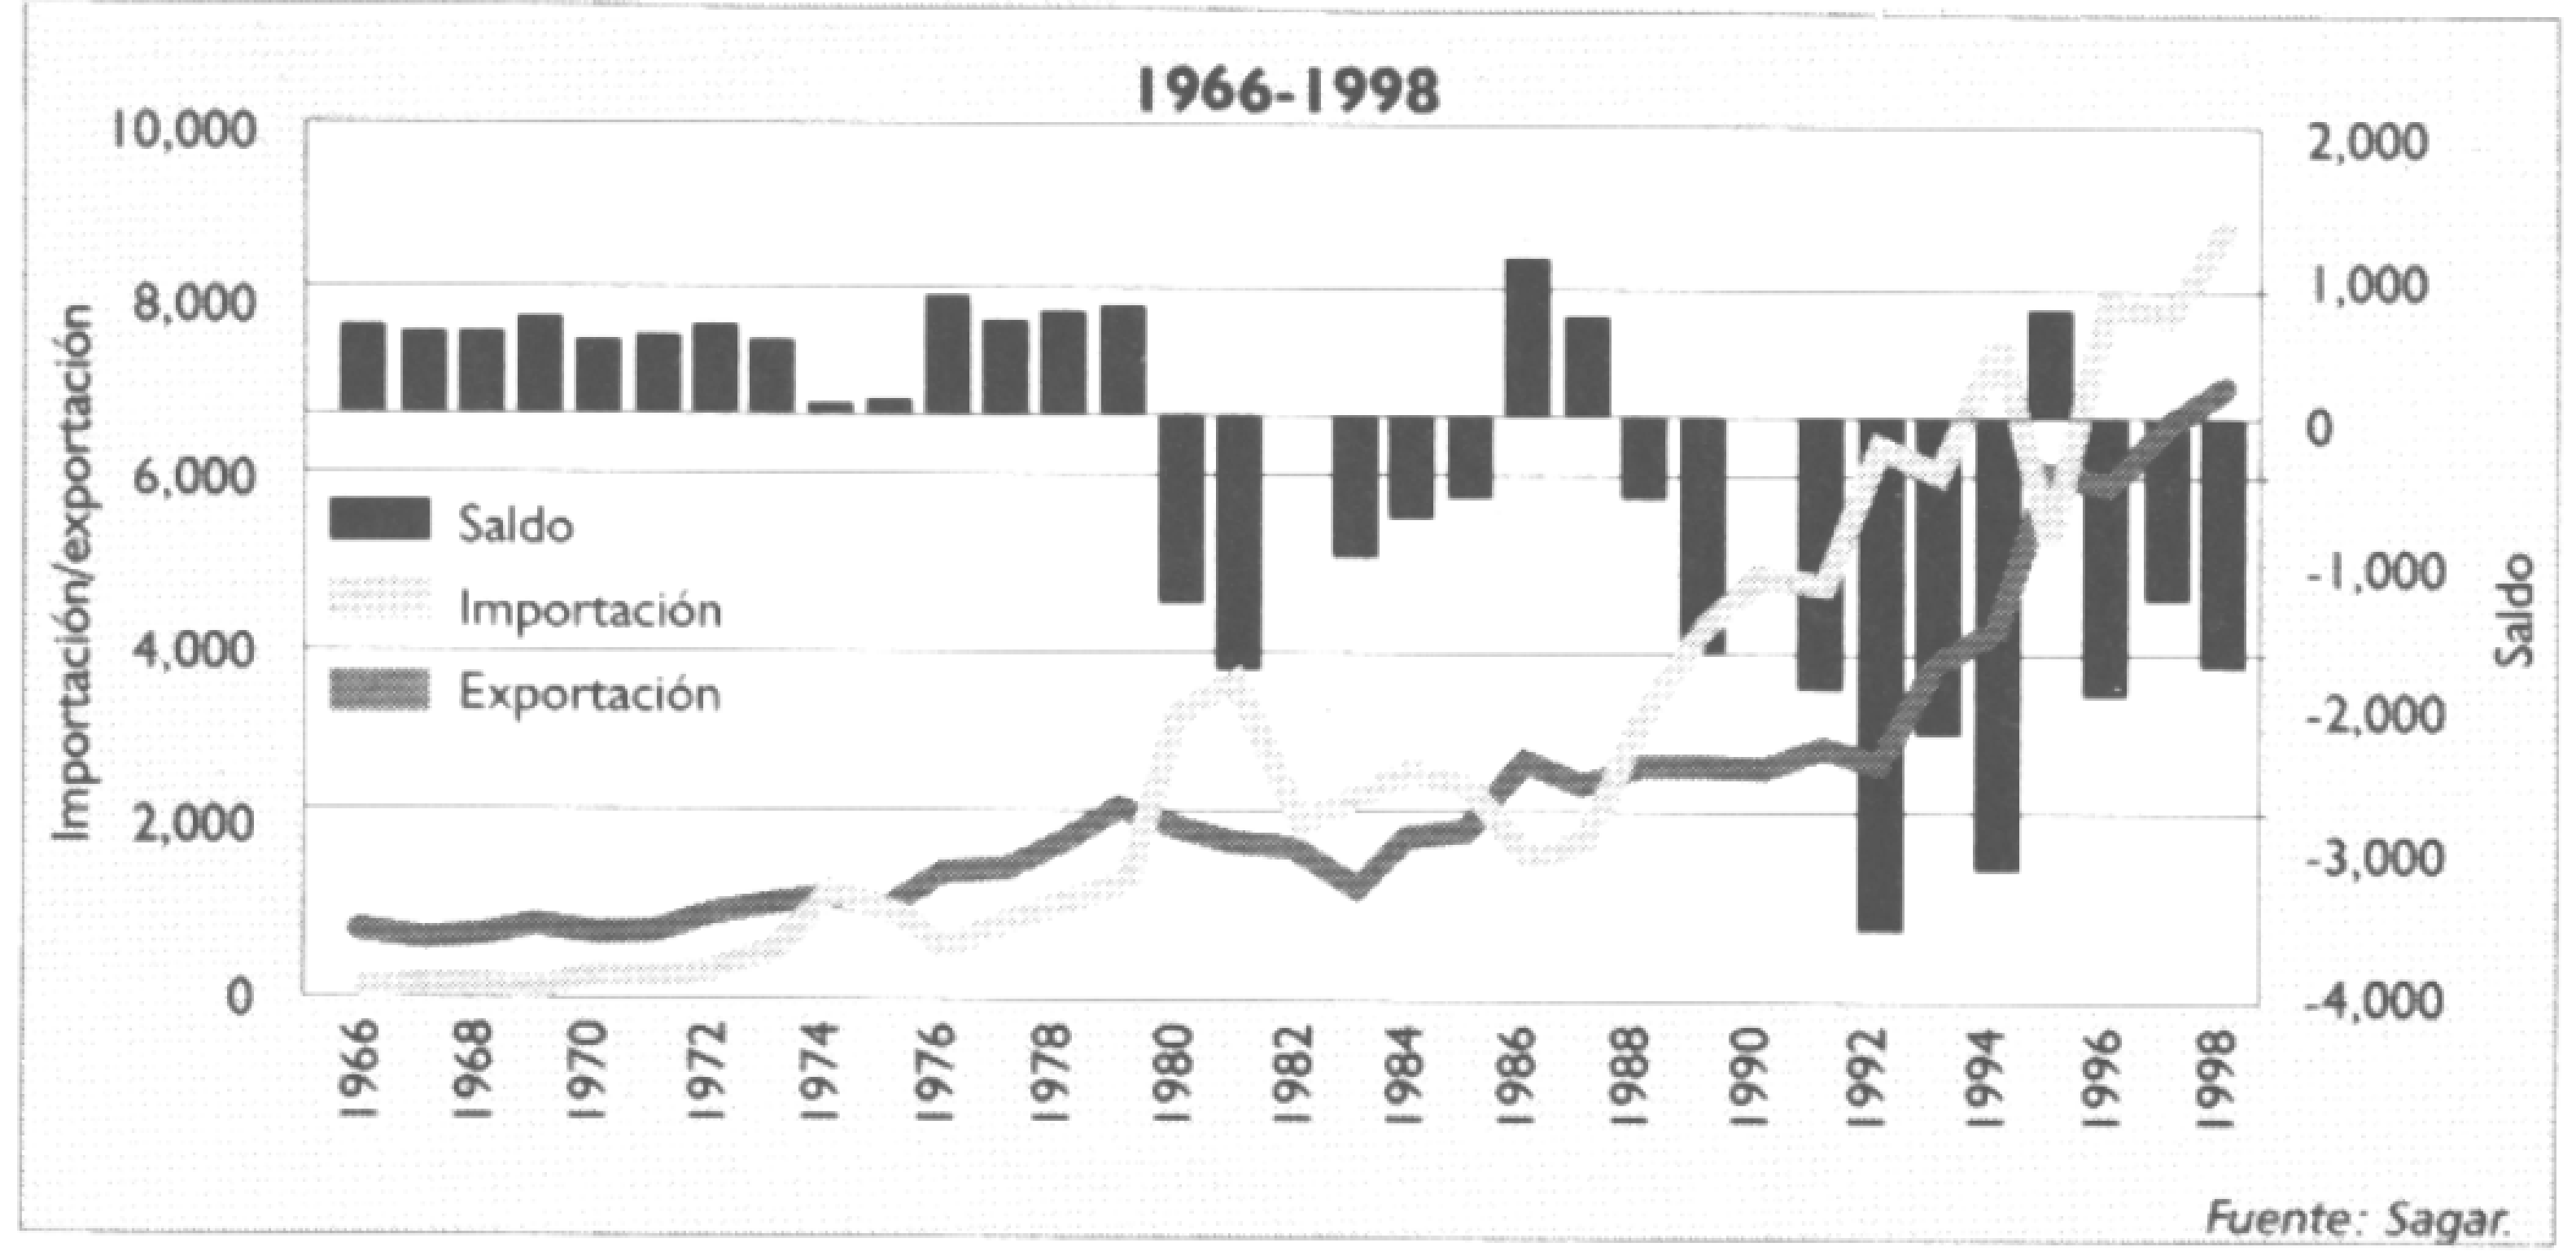
\includegraphics[width=0.7\textwidth]{fii6.png}}
	\caption{Balanza Comercial Agroalimentaria de México durante el periodo
		1966-1998 (en millones de dólares)}
	\label{fii6}
\end{figure}

\section{Manejo del agua}
El agua superficial consta de dos cuerpos distintos de agua en la naturaleza:
\begin{enumerate}
	\item El agua oceánica, la cual se encuentra altamente mineralizada por sales. El
	      cuerpo de agua oceánica contiene agua para cubrir todo el globo terráqueo; es la
	      principal fuente de humedad atmosférica y, por ende, de los demás cuerpos de agua
	\item  Los cuerpos superficiales de agua dulce, que cubren pequeñas porciones de
	      la superficie terrestre.
\end{enumerate}

El agua dulce se halla en ríos, depósitos y lagos; es almacenada durante el
invierno como nieve o hielo.
Aún en regiones caracterizadas por abundantes cuerpos de agua superficial, la
mayoría de las plantas, y por lo tanto, el hombre, no vivirían si el agua almacenada del
suelo no fuera útil para la conservación de las plantas. Tomando como promedio 1.5 m
de espesor de la zona que penetran las raíces, la humedad contenida en el suelo es
equivalente a poco menos de 30 cm de agua. El agua almacenada en el suelo está
adherida a las partículas del mismo y es removida en gran parte por la transpiración de
las plantas. Este déficit o pérdida debe ser repuesto antes de que el agua se pueda
mover hacia abajo, hasta el espejo del agua a través de la zona vacía del suelo. Por
consiguiente, la filtración del agua de lluvia no puede ser una fuente importante del
agua en regiones áridas.

La manifestación del agua superficial que permite ser aprovechada en lugares
alejados a donde se encuentra como ejemplo el caso de lagos y lagunas, es a través
del escurrimiento que se presenta en cauces de ríos o arroyos. El escurrimiento es el
agua proveniente de la precipitación que circula sobre o bajo la capa superficial del
suelo o en estratos más profundos y que llega a una corriente para finalmente ser
drenada hasta la salida de una cuenca. Existen tres tipos de escurrimiento: superficial,
subsuperficial y subterráneo.

La forma de aprovechar el agua superficial, en forma de escurrimiento, es a
través de diferentes obras de infraestructura que van a estar condicionadas a la forma
como se de el escurrimiento en los cauces, así si el escurrimiento es intermitente,
situación típica de zonas áridas y semiáridas, la forma de aprovechar esto es a través
de presas de almacenamiento auxiliadas con otras obras; si el escurrimiento es
permanente y este es de magnitud pequeña en la época de estiaje, la forma de
aprovechar este es a través de Presas derivadoras, situación típica en zonas
semihúmedas, y si el escurrimiento es permanente y la magnitud de este es de gran
tamaño, la forma de aprovechar estos es a través de tomas directas, esto es típico en
zonas húmedas.

\textbf{El almacenamiento de agua depende:}
\begin{itemize}
	\item Área y forma de la cuenca
	\item Precipitación en la cuenca (registros necesarios: Estaciones termopluviométricas)
	\item Escurrimientos superficiales (registros necesarios: Estaciones hidrométricas)
	\item Carácter geológico del sitio.
\end{itemize}

\textbf{Tipos de almacenamiento:}
\begin{itemize}
	\item Vasos en forma de lagos naturales (caso: Zacapu y Chapala, subirrigación)
	\item Vasos en cuencas de drenaje natural (presas de almacenamiento)
	\item Depresiones topográficas a las que debe conducirse el agua (importación de otra
	      cuenca)
	\item Almacenamientos puramente artificiales (bordos, jagüeyes)
\end{itemize}

\textbf{Selección del sitio para un almacenamiento:}
\begin{itemize}
	\item Proximidad
	\item Abastecimiento
	\item Topografía
	\item Geología
\end{itemize}

\textbf{Precauciones especiales que se deben tener al planear almacenamientos:}
\begin{itemize}
	\item Evitar depósitos de yeso
	\item Grietas o cavidades en regiones volcánicas
	\item Atención a areniscas de grano grueso
	\item Depresiones con relleno de acarreo
	\item Rellenos de grava y arena
	\item Investigación completa para evaluar abastecimiento, determinar fugas posibles, evitar desbordamientos
	\item Estudio de los suelos superficiales y subsuelo del vaso y la cuenca (azolve).
	\item Probar alternativas de obras de excedencias.
	\item Protección de la cuenca tributaria, con manejo adecuado evitando y previniendo
	      la deforestación.
\end{itemize}

\subsection{Aprovechamientos de aguas subterráneas.}

Las aguas subterráneas tienen su origen en la precipitación y en la parte de la
misma que se denomina infiltración, que es el movimiento vertical del agua, a través de
las capas superficiales del suelo, producido por la acción de las fuerzas gravitacionales
y capilares. Este proceso se presenta en la capa superficial del suelo que se denomina:
``Zona de Fractura de las Rocas'' la cual a su vez se subdivide en tres capas: la primera
denominada de evaporación en la cual el movimiento del agua que se infiltra se
caracteriza por dos movimientos uno descendente y otro ascendente, el primero hace
que el agua siga su proceso hacia capas inferiores del suelo, y el segundo que hace
que regrese de nuevo a la atmósfera fundamentalmente en forma de vapor. La segunda
capa que se denomina zona de aireación, en la cual el agua se encuentra en
combinación con el aire ocupando los poros existentes en el suelo, con un solo
movimiento vertical descendente que hace que continué su camino hacia abajo, a la
siguiente capa, que se denomina zona de saturación, en la cual el aire desaparece de
los poros y el agua ocupa exclusivamente el espacio que ellos dejan, conformando en
su parte superior lo que se denomina nivel freático, y en su parte inferior lo que se
denomina hidroapoyo concluyendo con la zona de fractura de las rocas, tal como se
observa en la Figura \ref{fii7}.


\begin{figure}[h!]
	\centering
	\begin{subfigure}[b]{0.45\linewidth}
		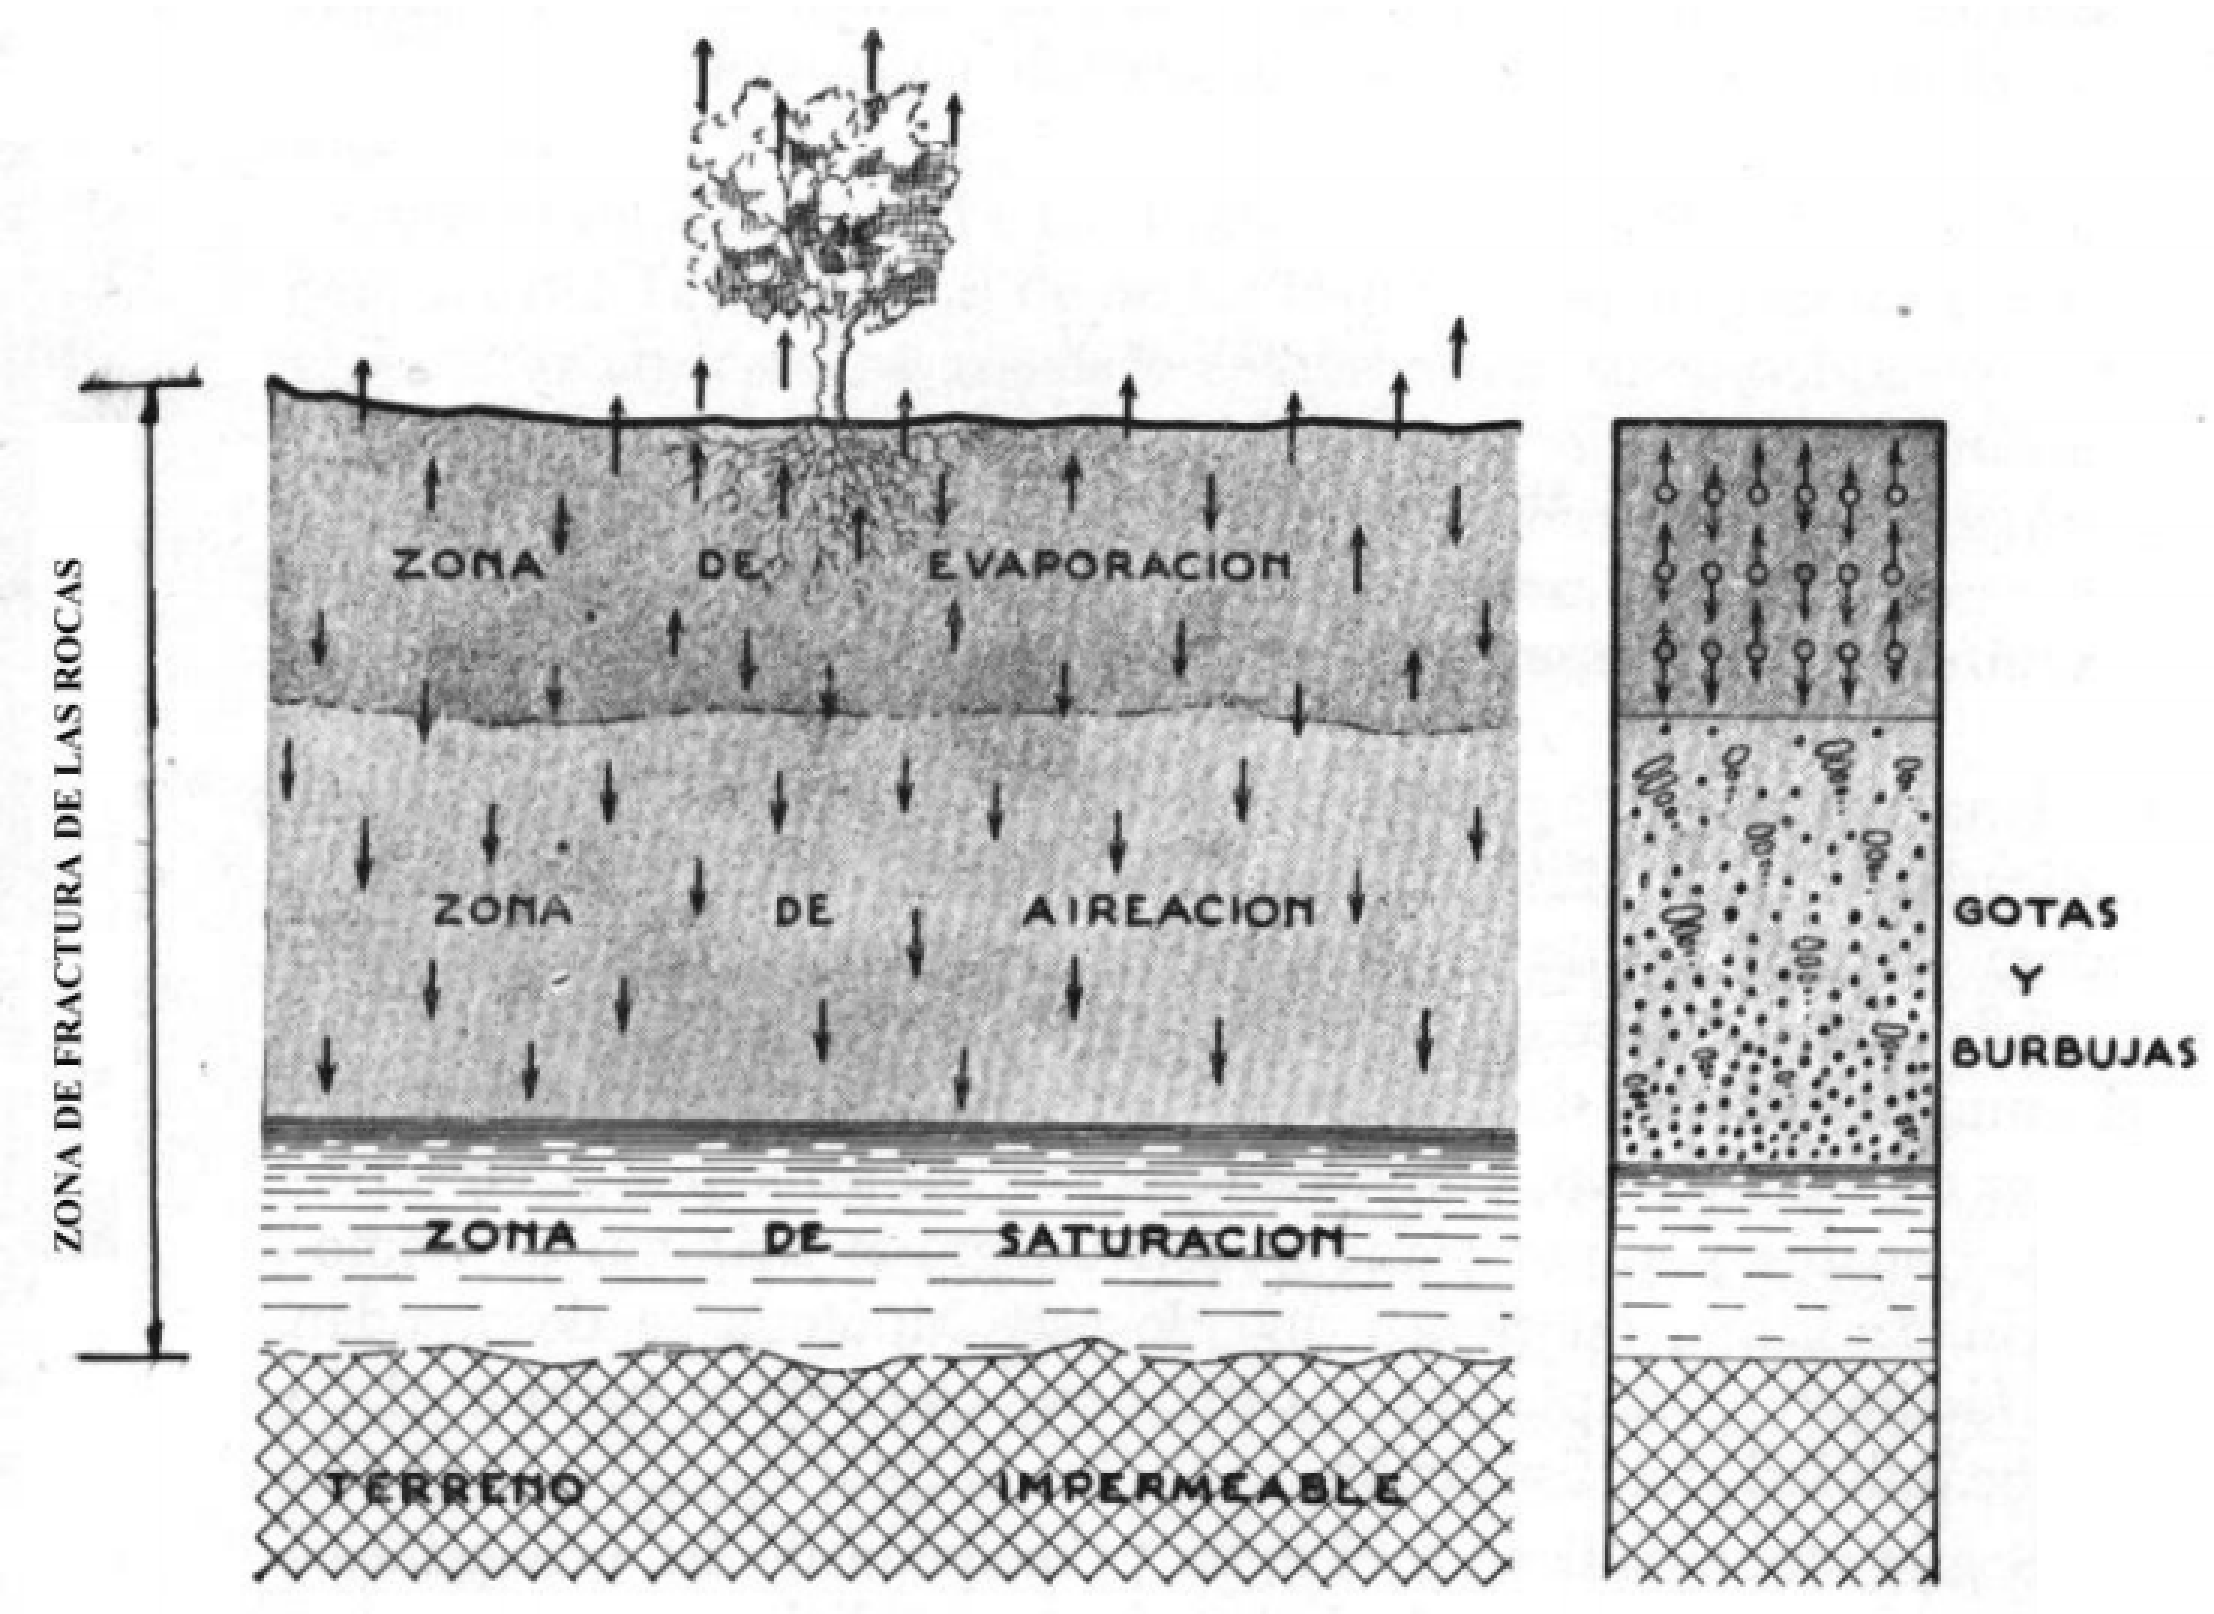
\includegraphics[width=\linewidth]{fii7.png}
		\caption{Capa superficial del movimiento del agua subterránea.}
		\label{fii7}
	\end{subfigure}
	\begin{subfigure}[b]{0.45\linewidth}
		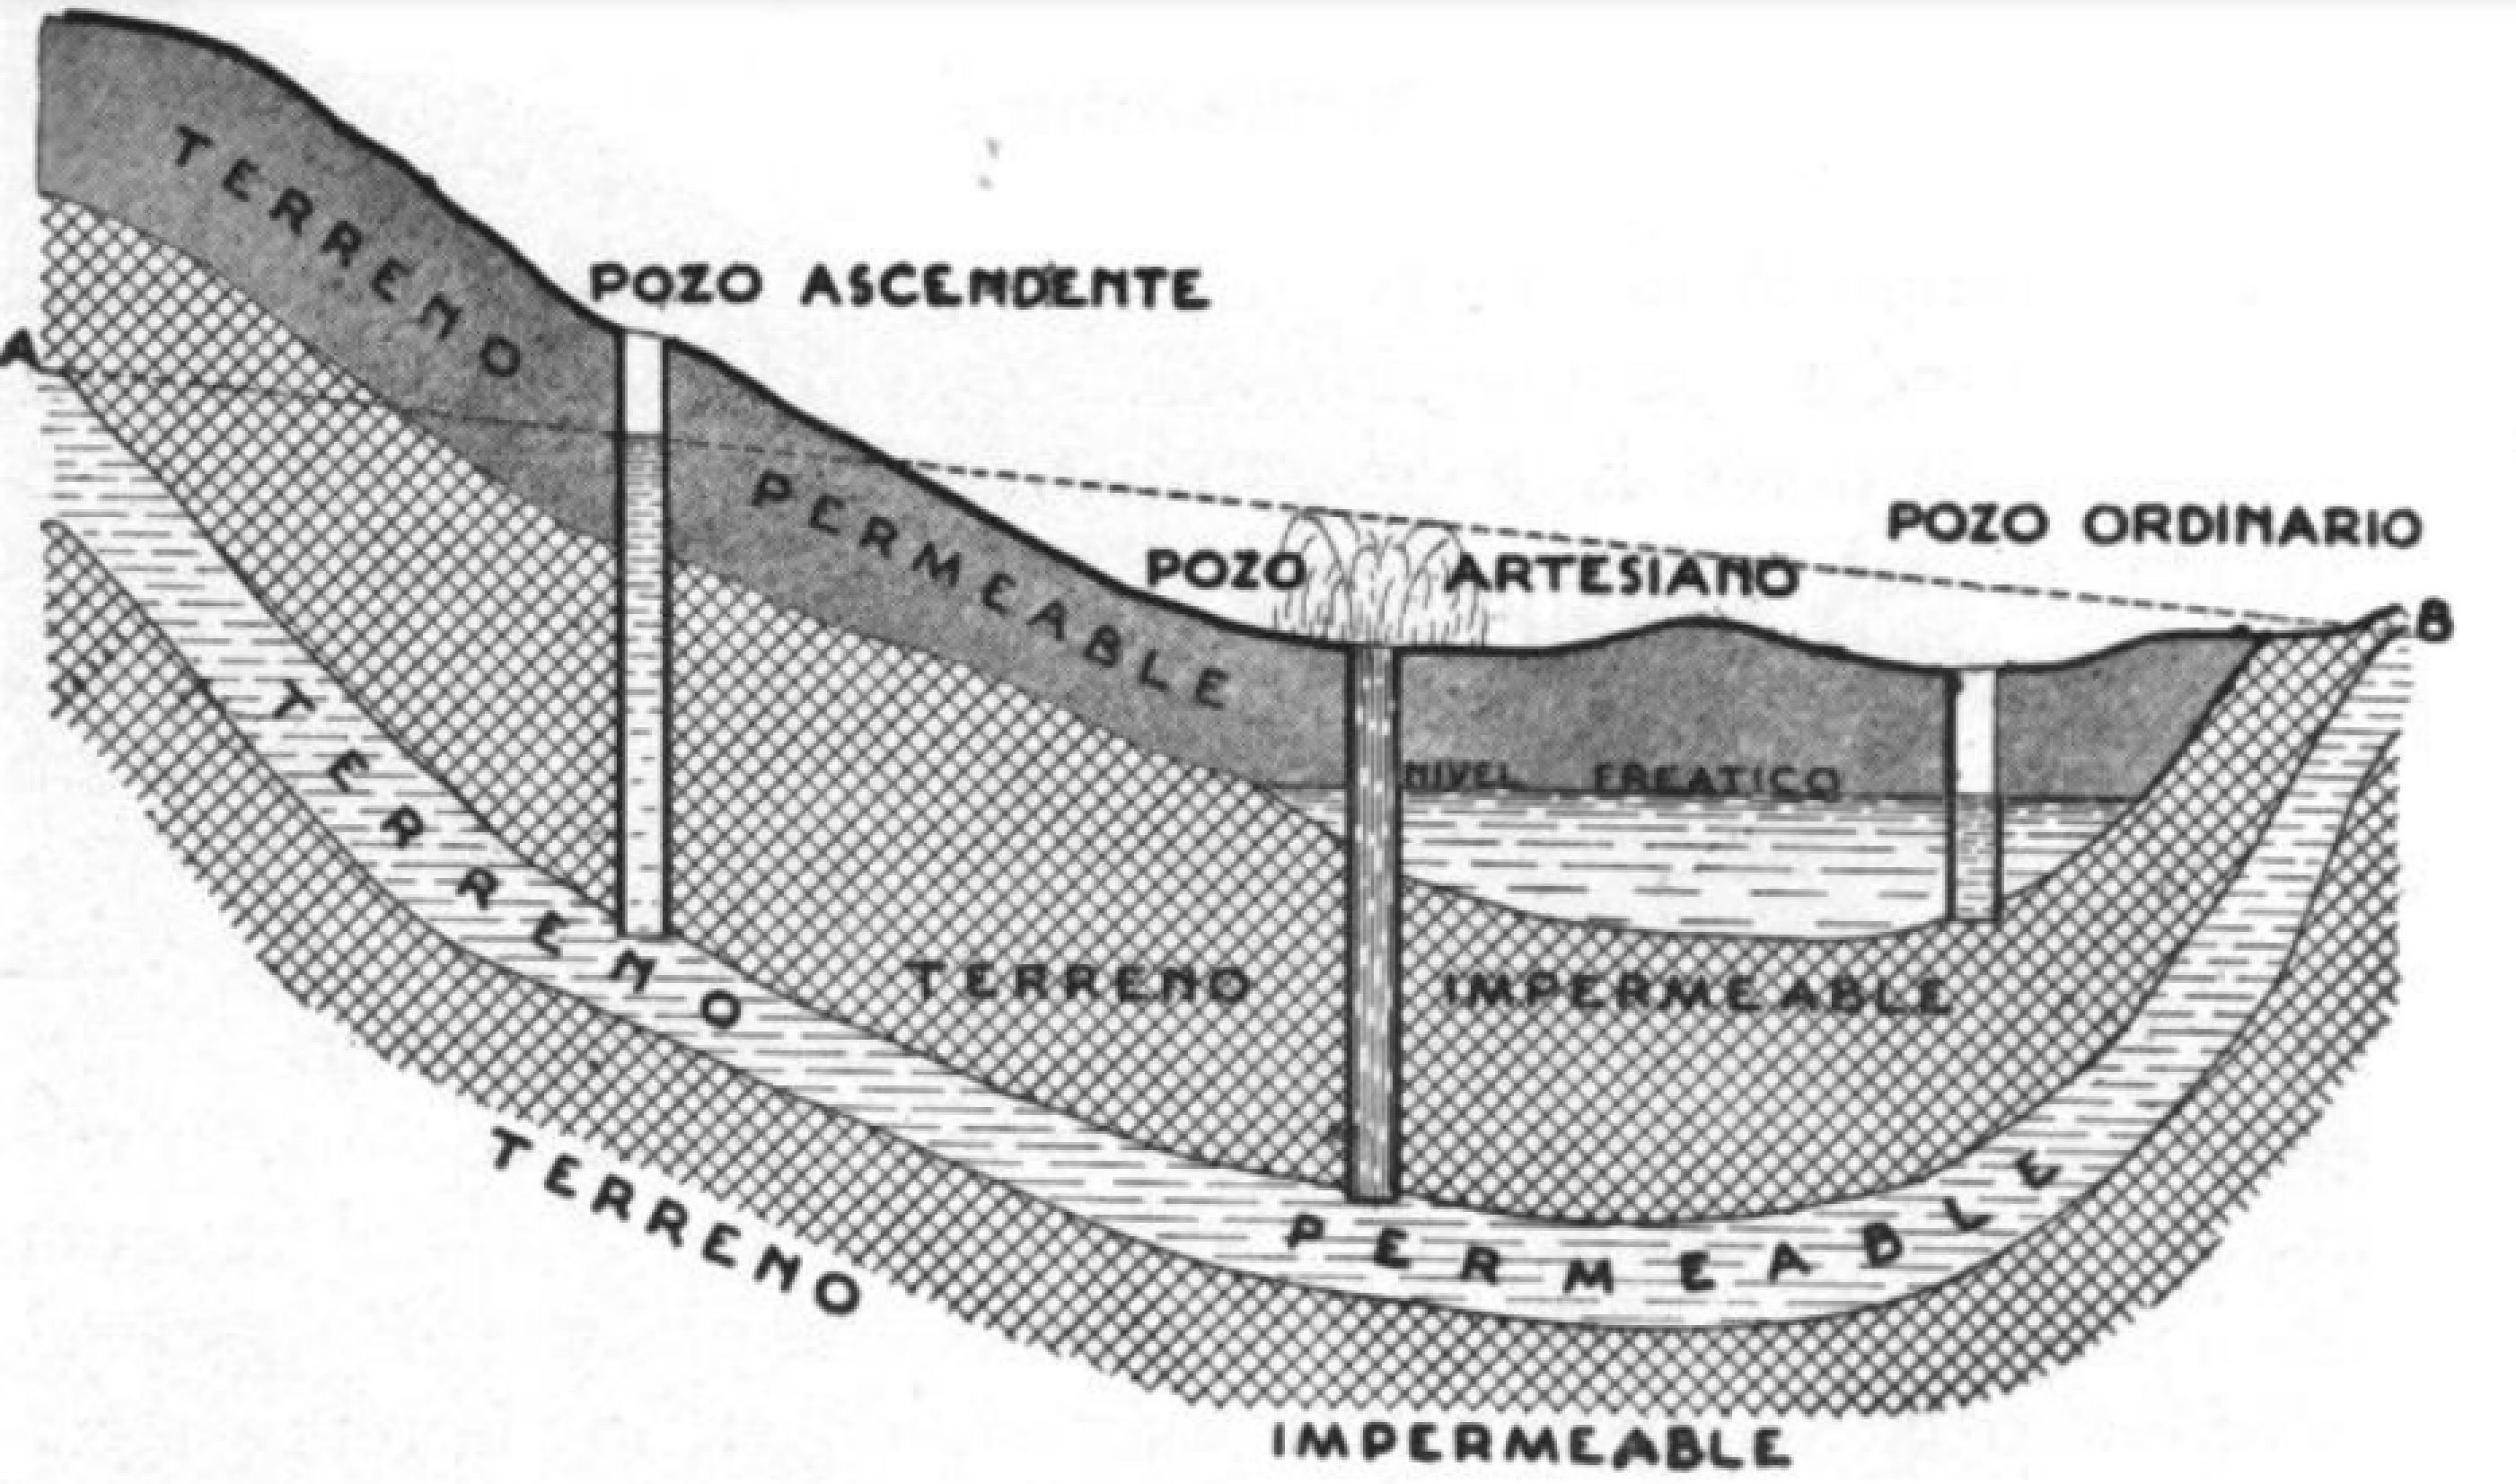
\includegraphics[width=\linewidth]{fii8.png}
		\caption{El punto de salida está dentro de los límites de la cuenca y generalmente es un lago.}
		\label{fii8}
	\end{subfigure}
	\caption{Formas de explotación artificial de las aguas subterráneas.}
	\label{fig7-8}
\end{figure}

\subsubsection{Tipos de alumbramiento de las aguas subterráneas.}

\begin{enumerate}
	\item Alumbramiento natural.
	      \begin{enumerate}
		      \item  Manantiales o fuentes
		            \begin{enumerate}
			            \item De afloramiento, derramamiento o vertedero.
			            \item De emergencia o de vaguada
			            \item De grieta o de filón
			            \item Intermitentes
			            \item  Intercalares
		            \end{enumerate}
	      \end{enumerate}
	\item Alumbramiento artificial
	      \begin{enumerate}
		      \item  Sentido vertical (pozos)
		            \begin{enumerate}
			            \item Pequeño diámetro (pozos profundos, taladros, perforaciones o
			                  pozos entubados).
			            \item Gran diámetro (a cielo abierto, pozos ordinarios o tipo noria).
			            \item Mixtos
		            \end{enumerate}
		      \item  Sentido horizontal (galerías).
		            \begin{enumerate}
			            \item Trincheras colectoras
			            \item Galerías filtrantes
			            \item Galerías de captación
			            \item Galerías en el fondo de pozos.
		            \end{enumerate}
	      \end{enumerate}
\end{enumerate}

\begin{figure}[h!]
	\centering
	\begin{subfigure}[b]{0.4\linewidth}
		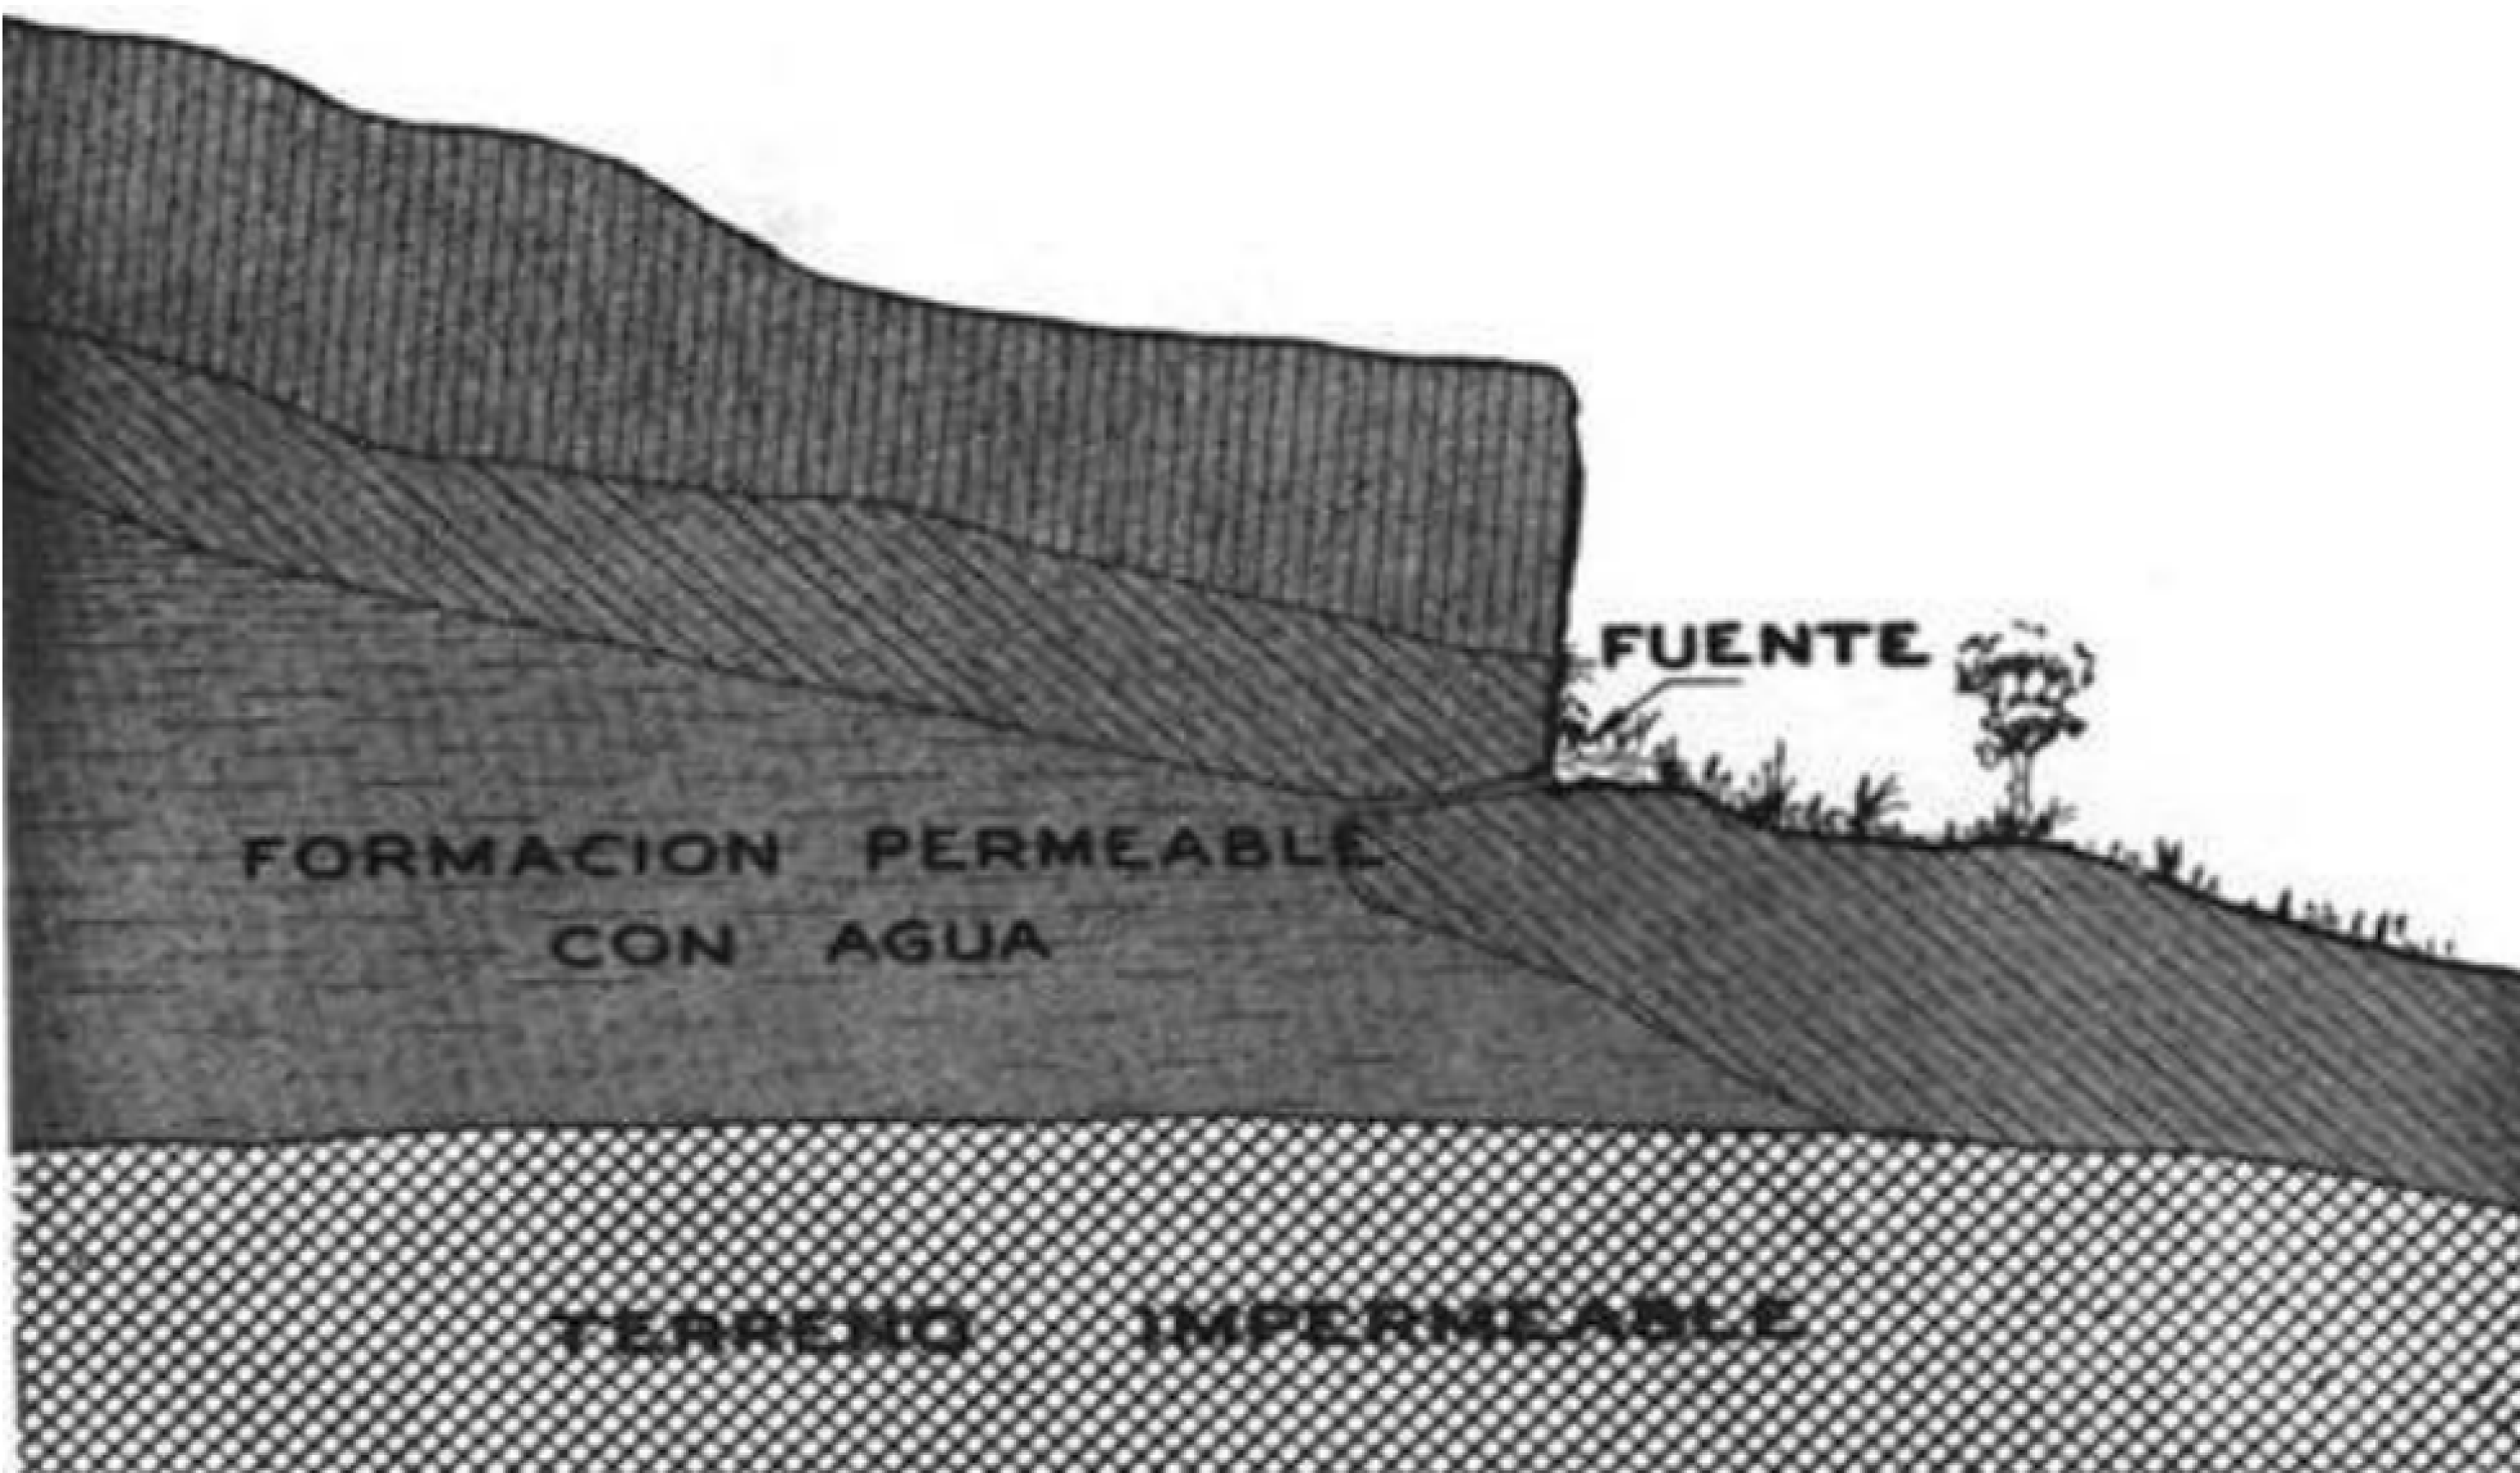
\includegraphics[width=\linewidth]{fii9.png}
		\caption{Manantial de afloramiento, en el que el agua mana como consecuencia
			de la carga a que está sometido, a través de una discontinuidad de la capa
			impermeable.}
		\label{fii9}
	\end{subfigure}
	\begin{subfigure}[b]{0.4\linewidth}
		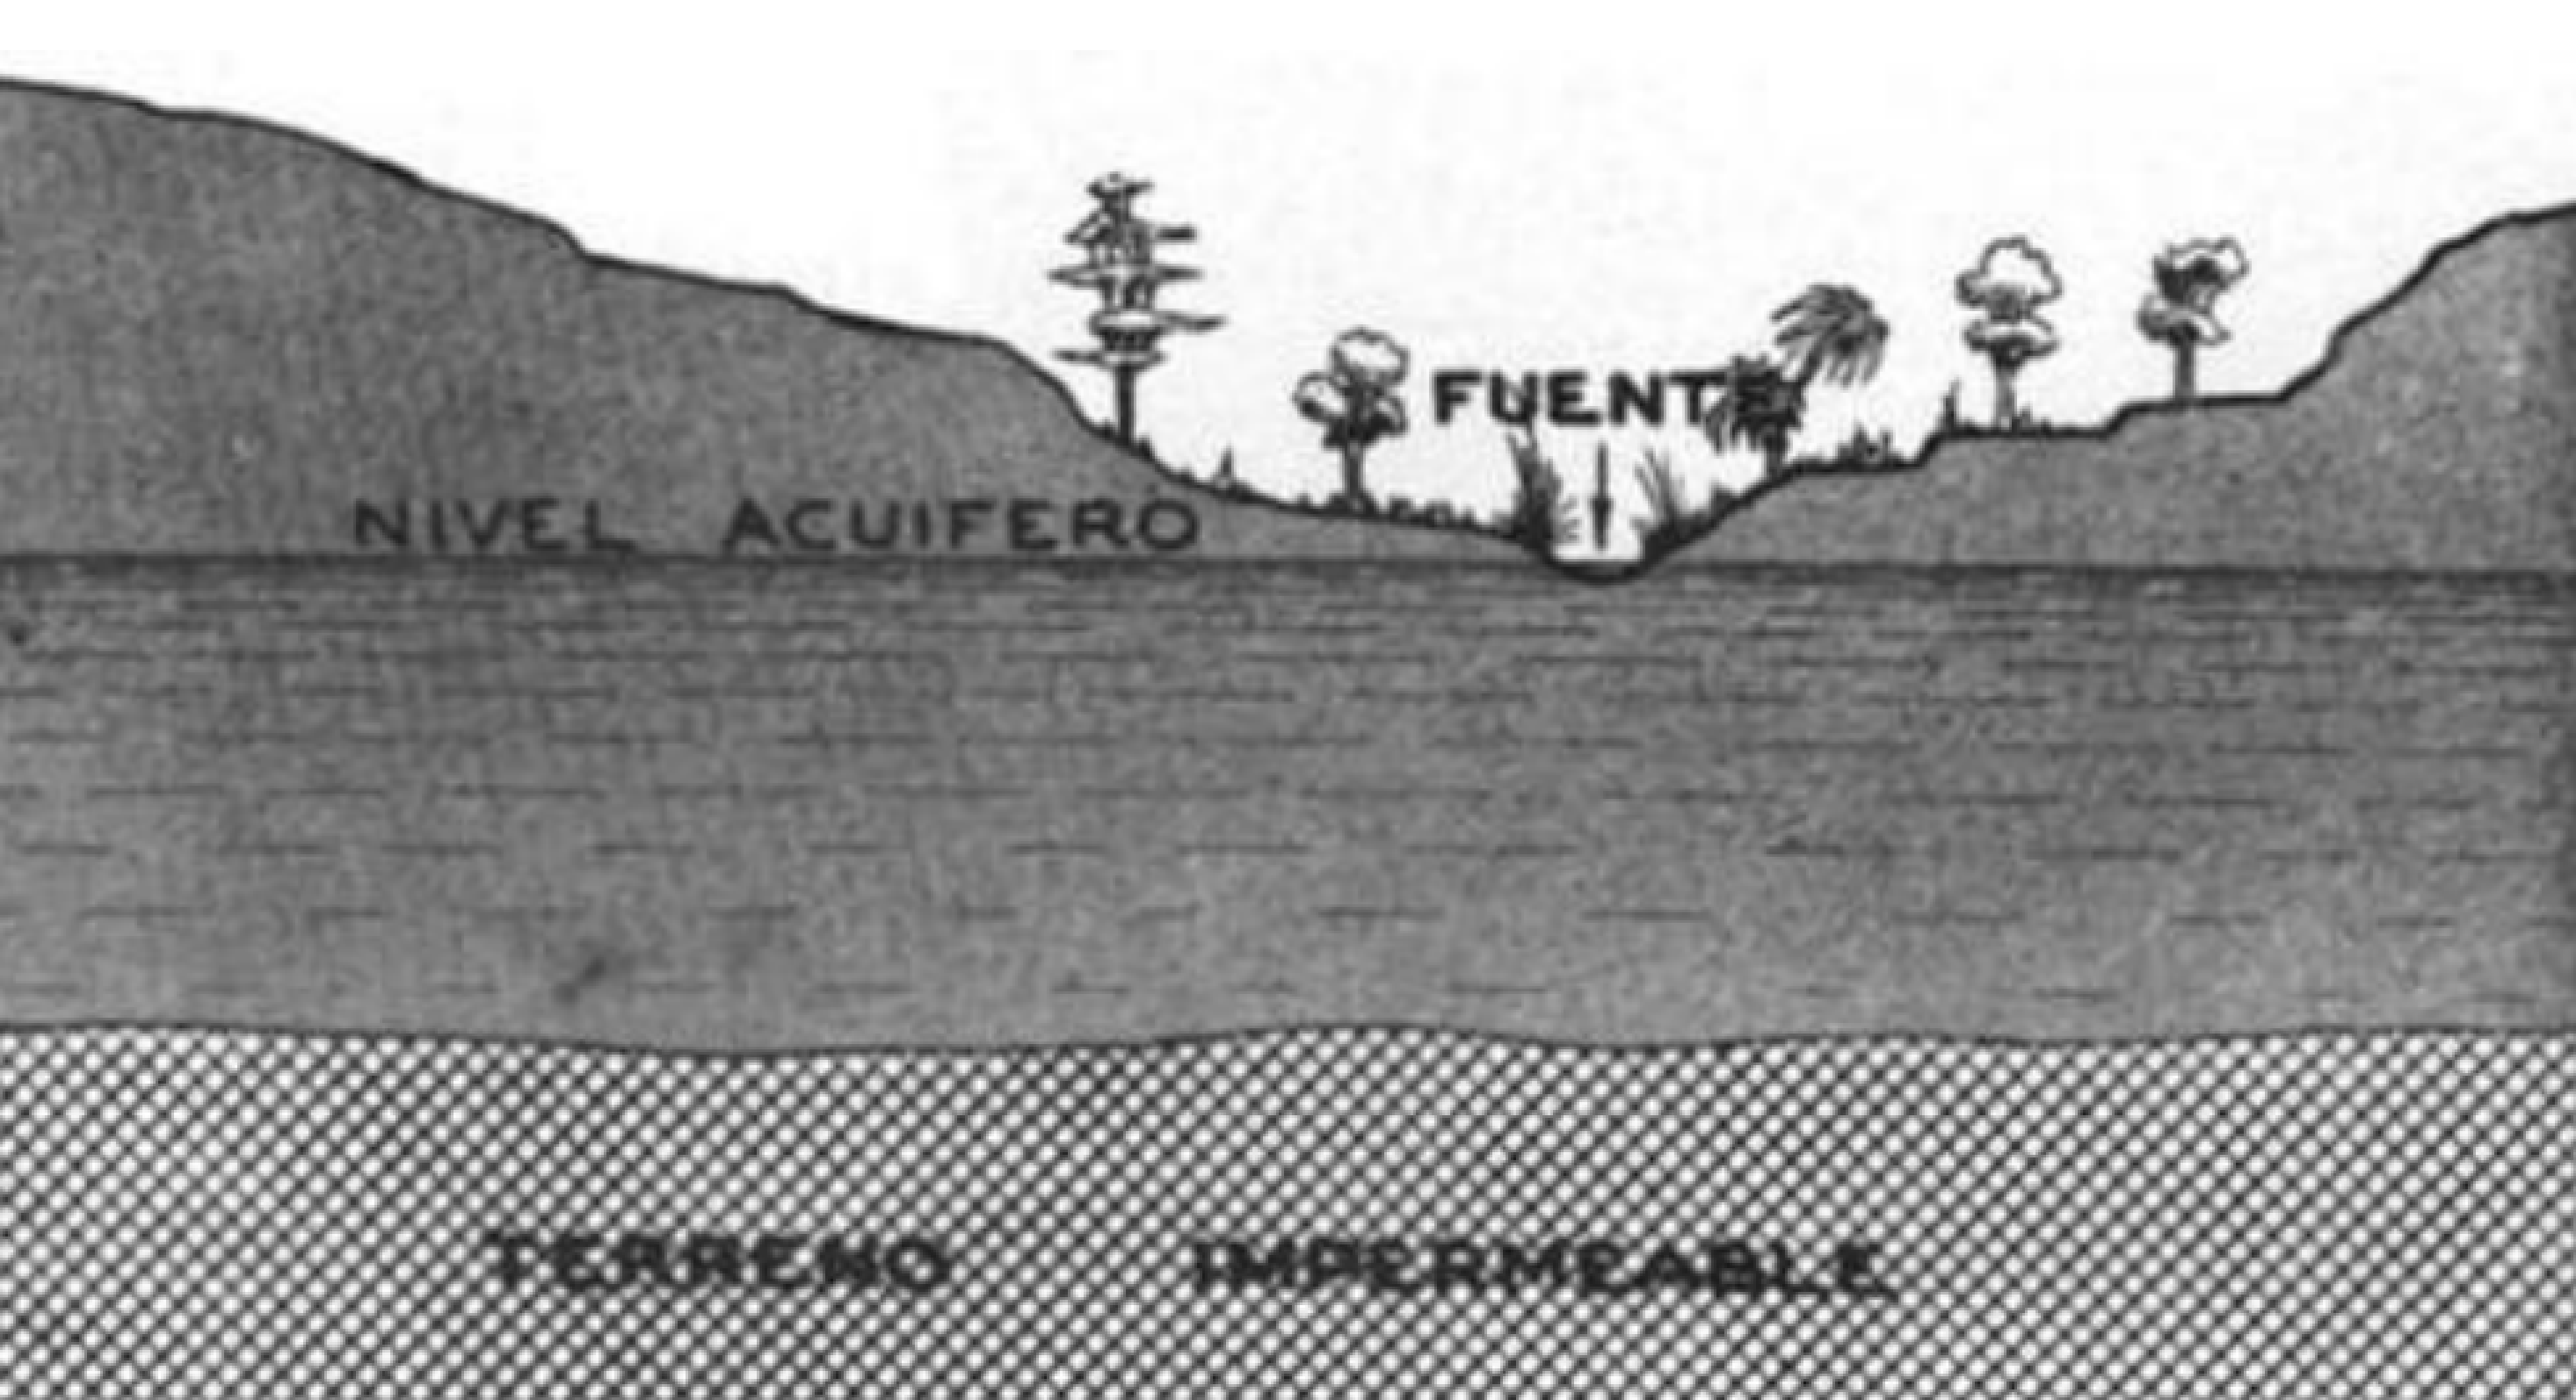
\includegraphics[width=\linewidth]{fii10.png}
		\caption{ Manantial de vaguada, debido a la existencia de una depresión del
			terreno por debajo del nivel del acuífero.}
		\label{fii10}
	\end{subfigure}
	\caption{Manantiales o fuentes}
	\begin{subfigure}[b]{0.4\linewidth}
		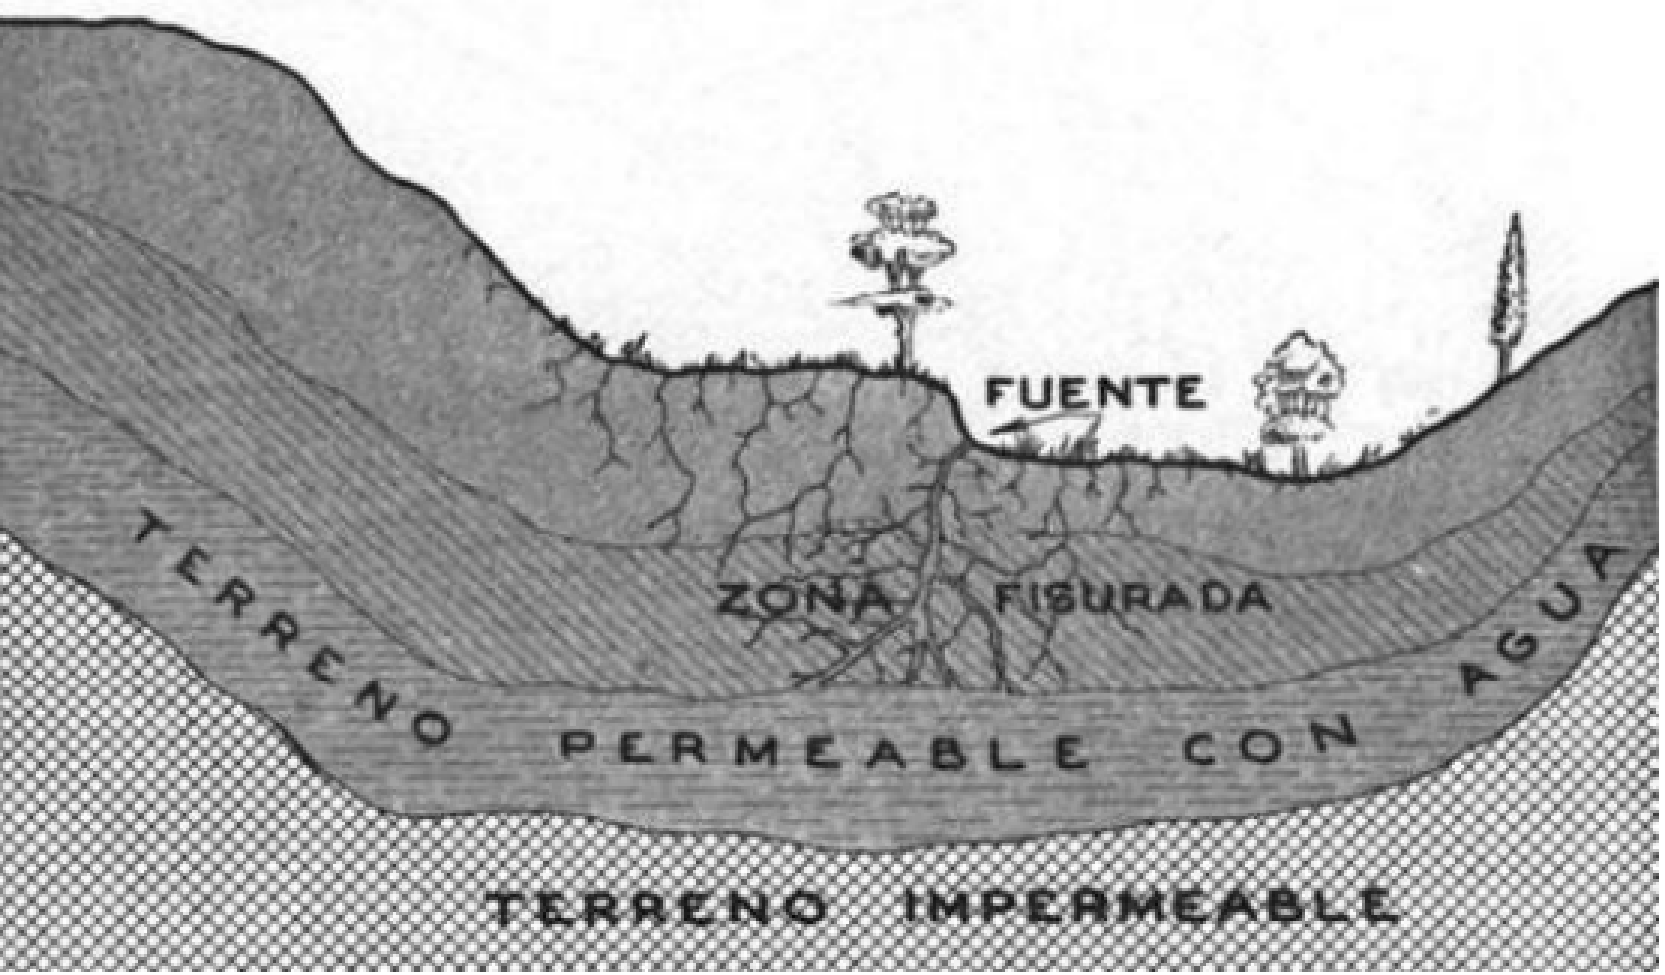
\includegraphics[width=\linewidth]{fii11.png}
		\caption{Manantial de grieta o de filón, el cual mana a través de una
			formación fisurada y cuyas aguas proceden de un manto profundo, a veces
			termal.}
		\label{fii11}
	\end{subfigure}
	\begin{subfigure}[b]{0.4\linewidth}
		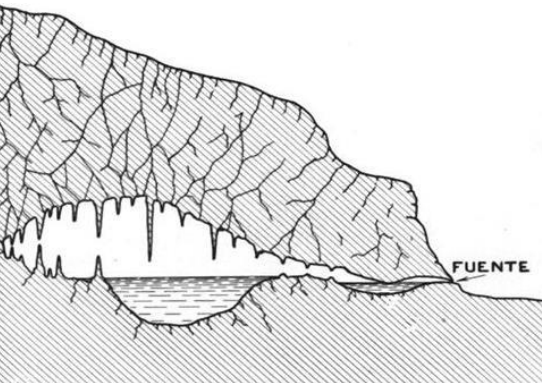
\includegraphics[width=\linewidth]{fii12.png}
		\caption{ Manantial intermitente, el cual cesa de manar cuando alcanza cierta
			altura el agua en el depósito subterráneo que lo alimenta.}
		\label{fii12}
	\end{subfigure}
	\caption{Manantiales o fuentes}
	\label{fig9-12}
\end{figure}

\begin{figure}
	\centerline{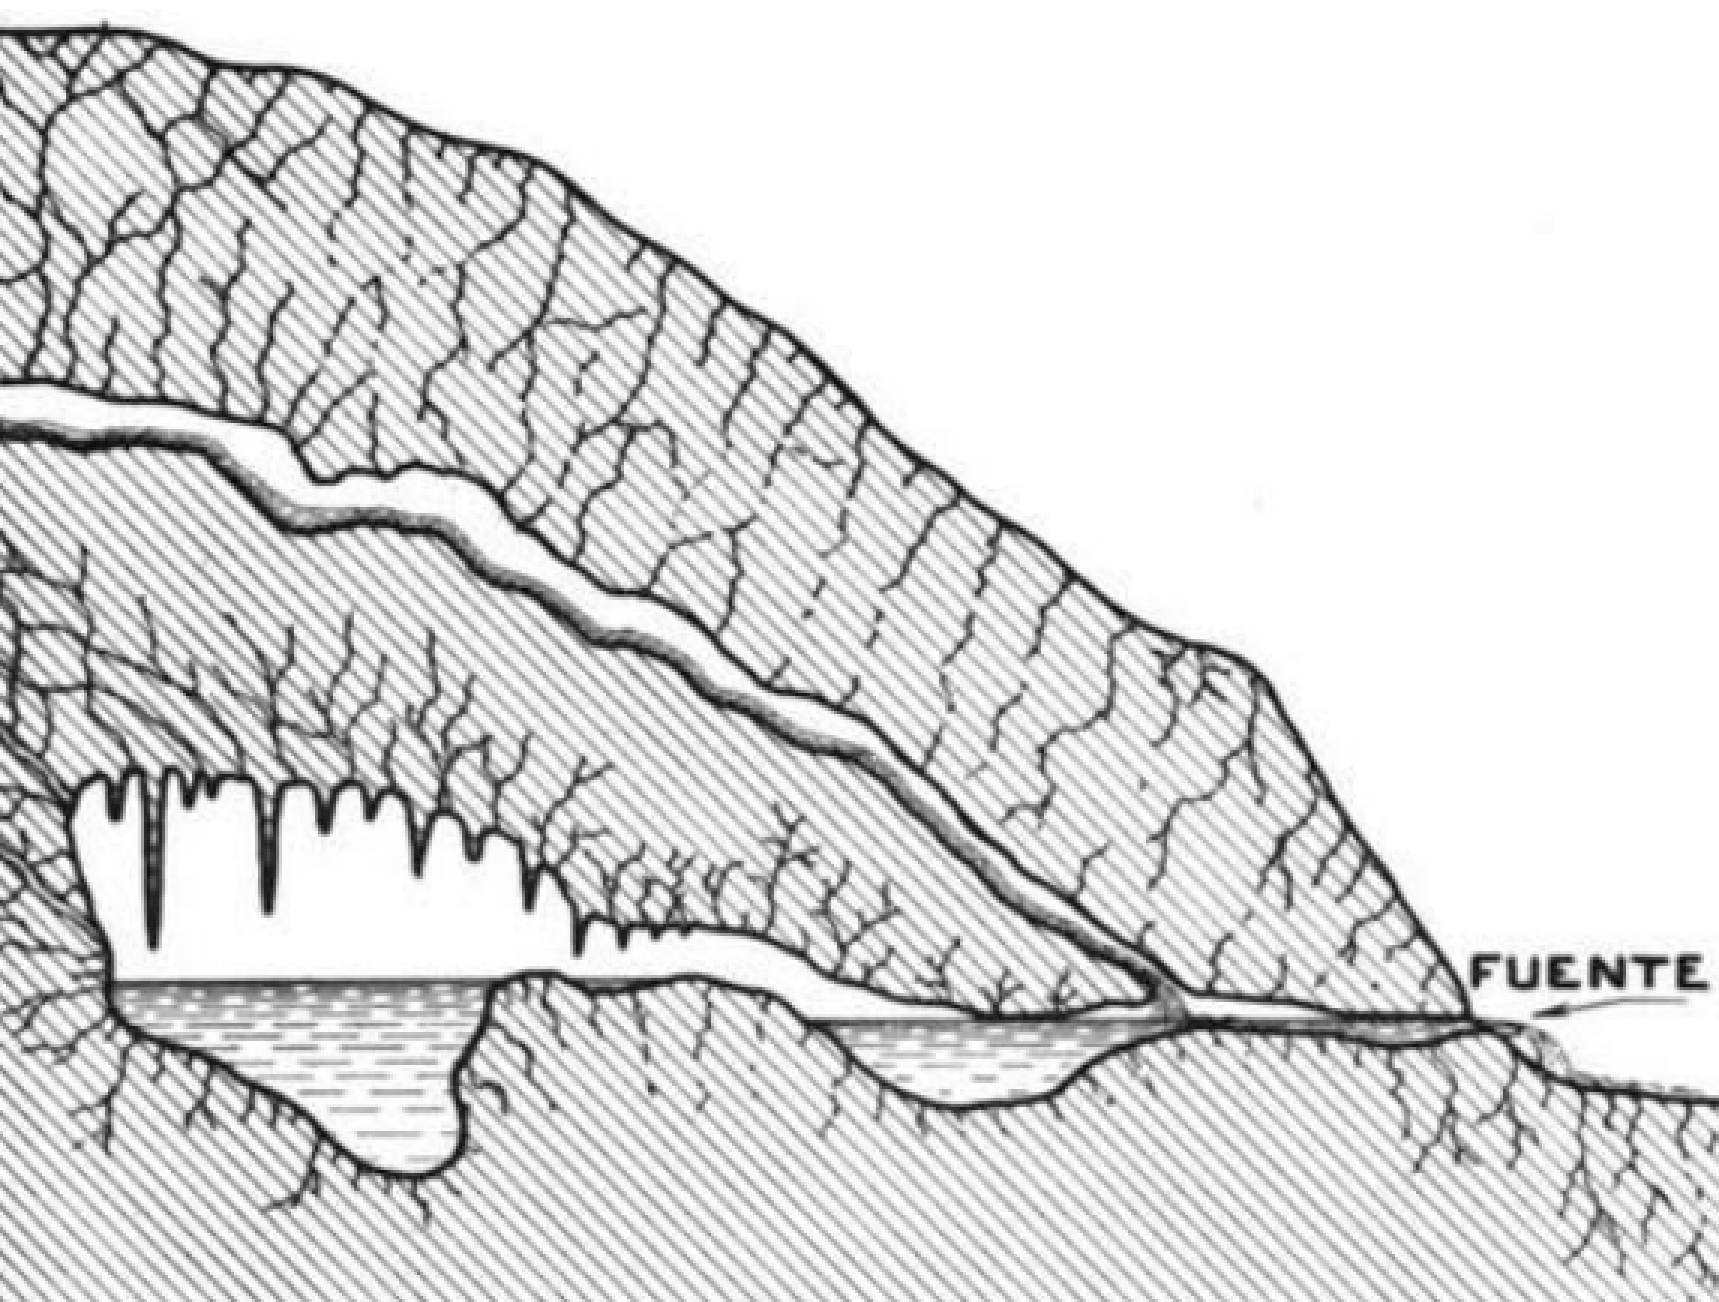
\includegraphics[width=0.5\textwidth]{fii13.png}}
	\caption{manantial intercalar, que ofrece variaciones de gastos por la
		coexistencia de un depósito de intermitencia y de una alimentación continua.}
	\label{fii13}
\end{figure}

existen tres tipos de diámetros en los \textbf{pozos}, véase la figura \ref{fig14-17}:
\begin{enumerate}
	\item Pequeño diámetro: Diámetros de perforación de 5 a 60 cm de forma circular.
	\item De gran diámetro: Diámetros de excavación de 1 a 5 m en formas circular, rectangular y
	      elíptica
	\item   Mixtos: Pozo de pequeño diámetro construido en uno de gran diámetro.
\end{enumerate}


\begin{figure}[h!]
	\centering
	\begin{subfigure}[b]{0.45\linewidth}
		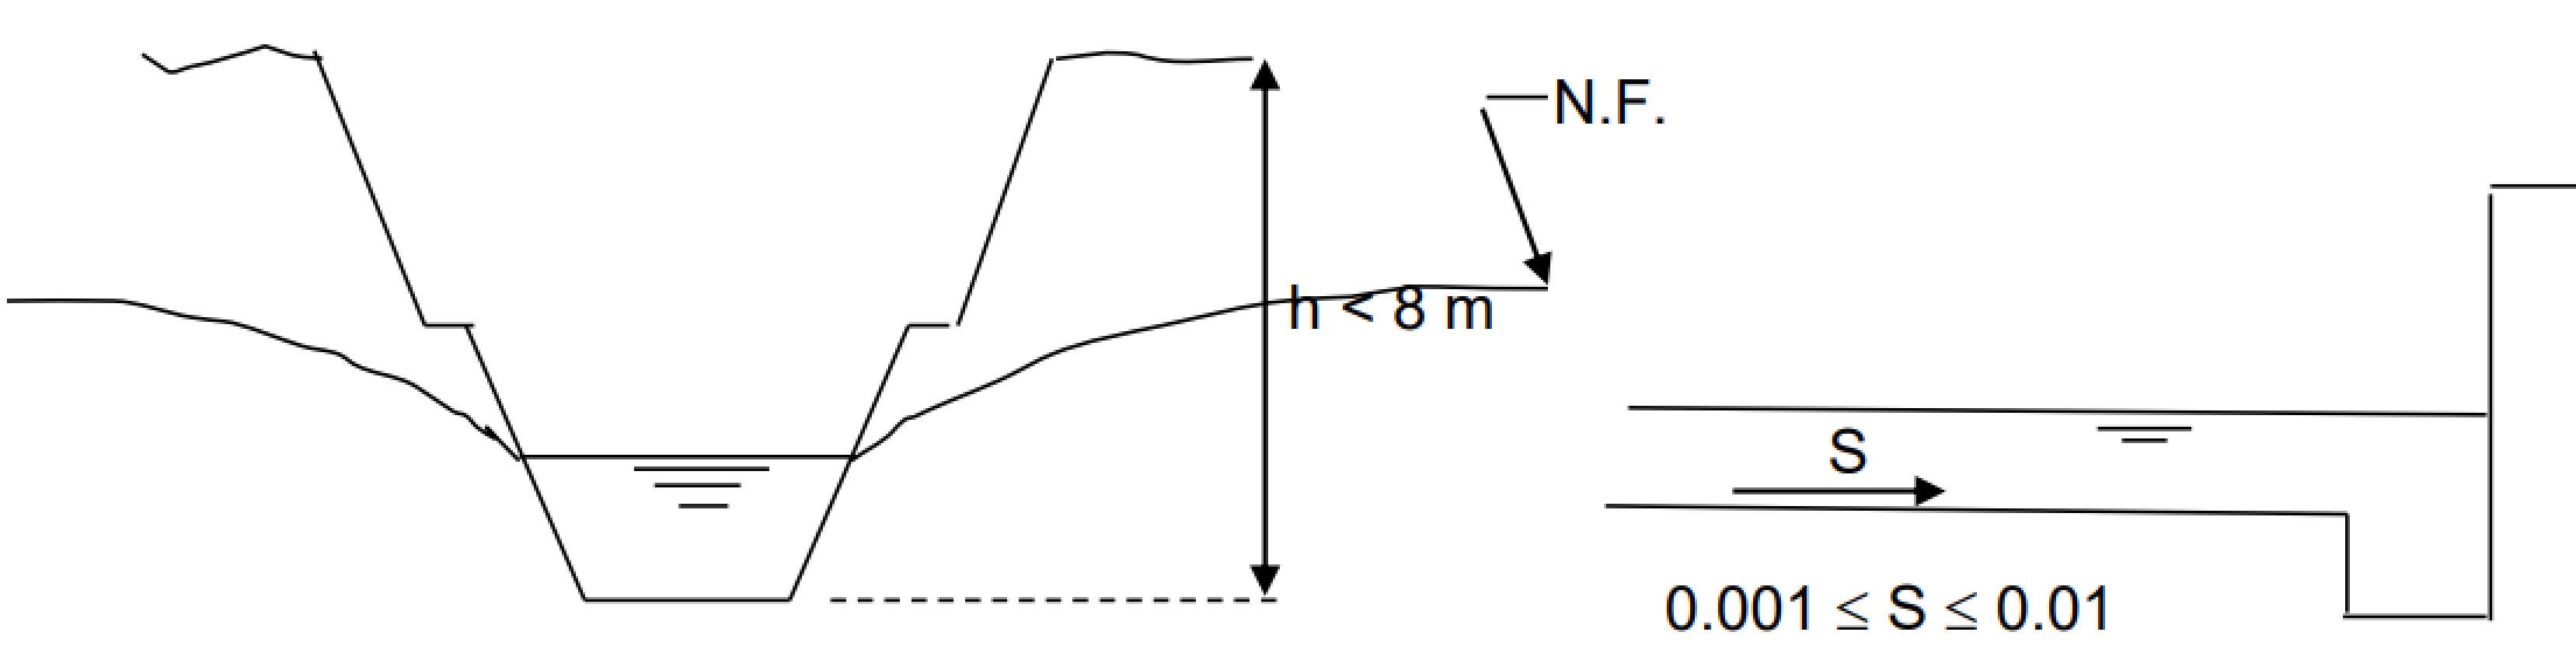
\includegraphics[width=\linewidth]{fii14.png}
		\caption{Trincheras colectoras}
		\label{fii14}
	\end{subfigure}
	\begin{subfigure}[b]{0.3\linewidth}
		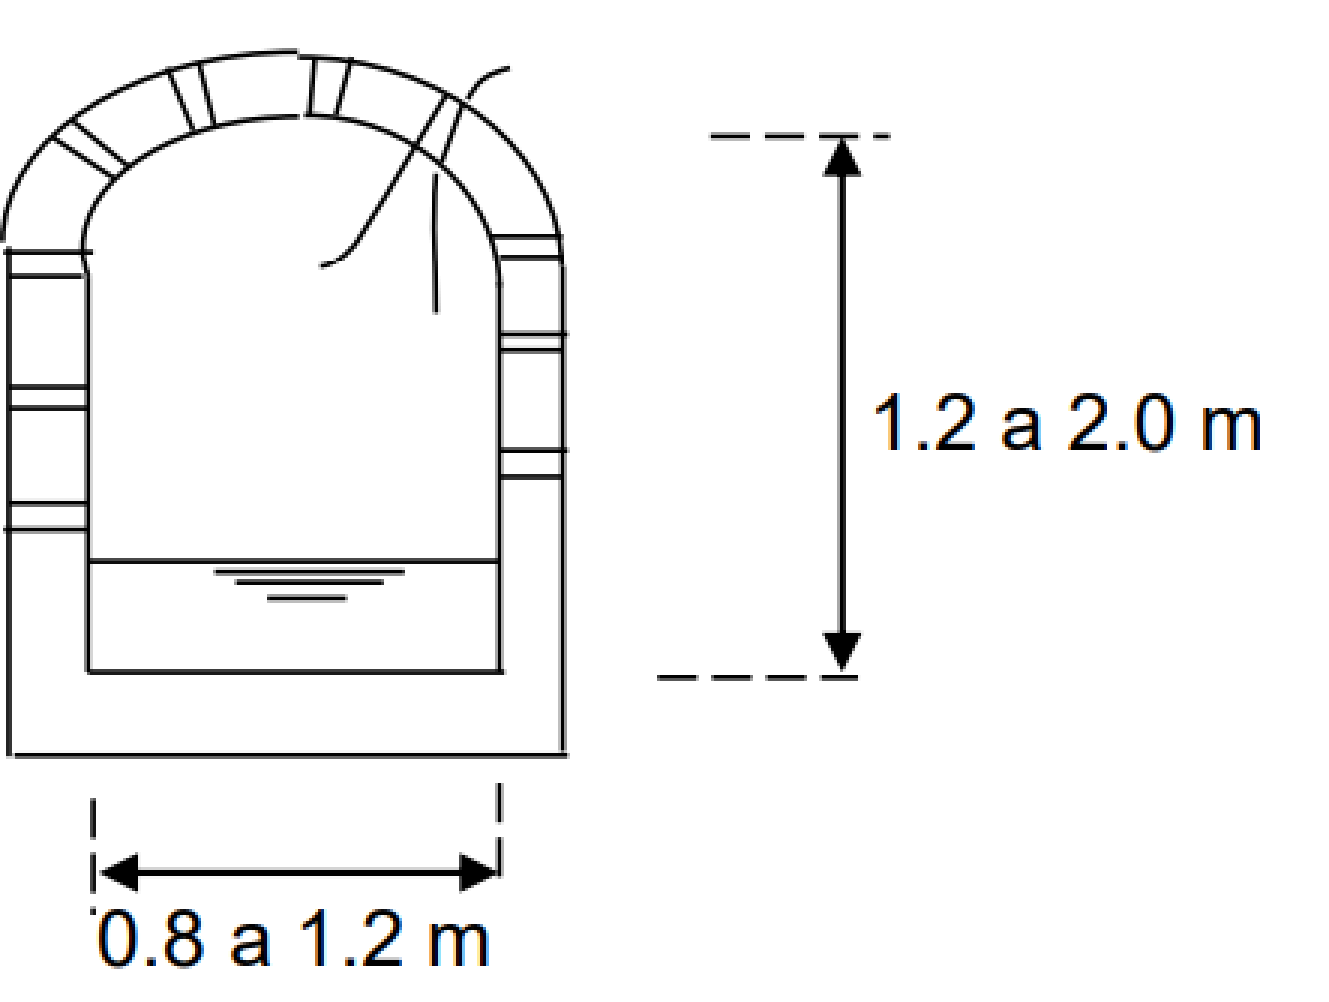
\includegraphics[width=\linewidth]{fii15.png}
		\caption{Galerías Filtrantes}
		\label{fii15}
	\end{subfigure}
	\begin{subfigure}[b]{0.45\linewidth}
		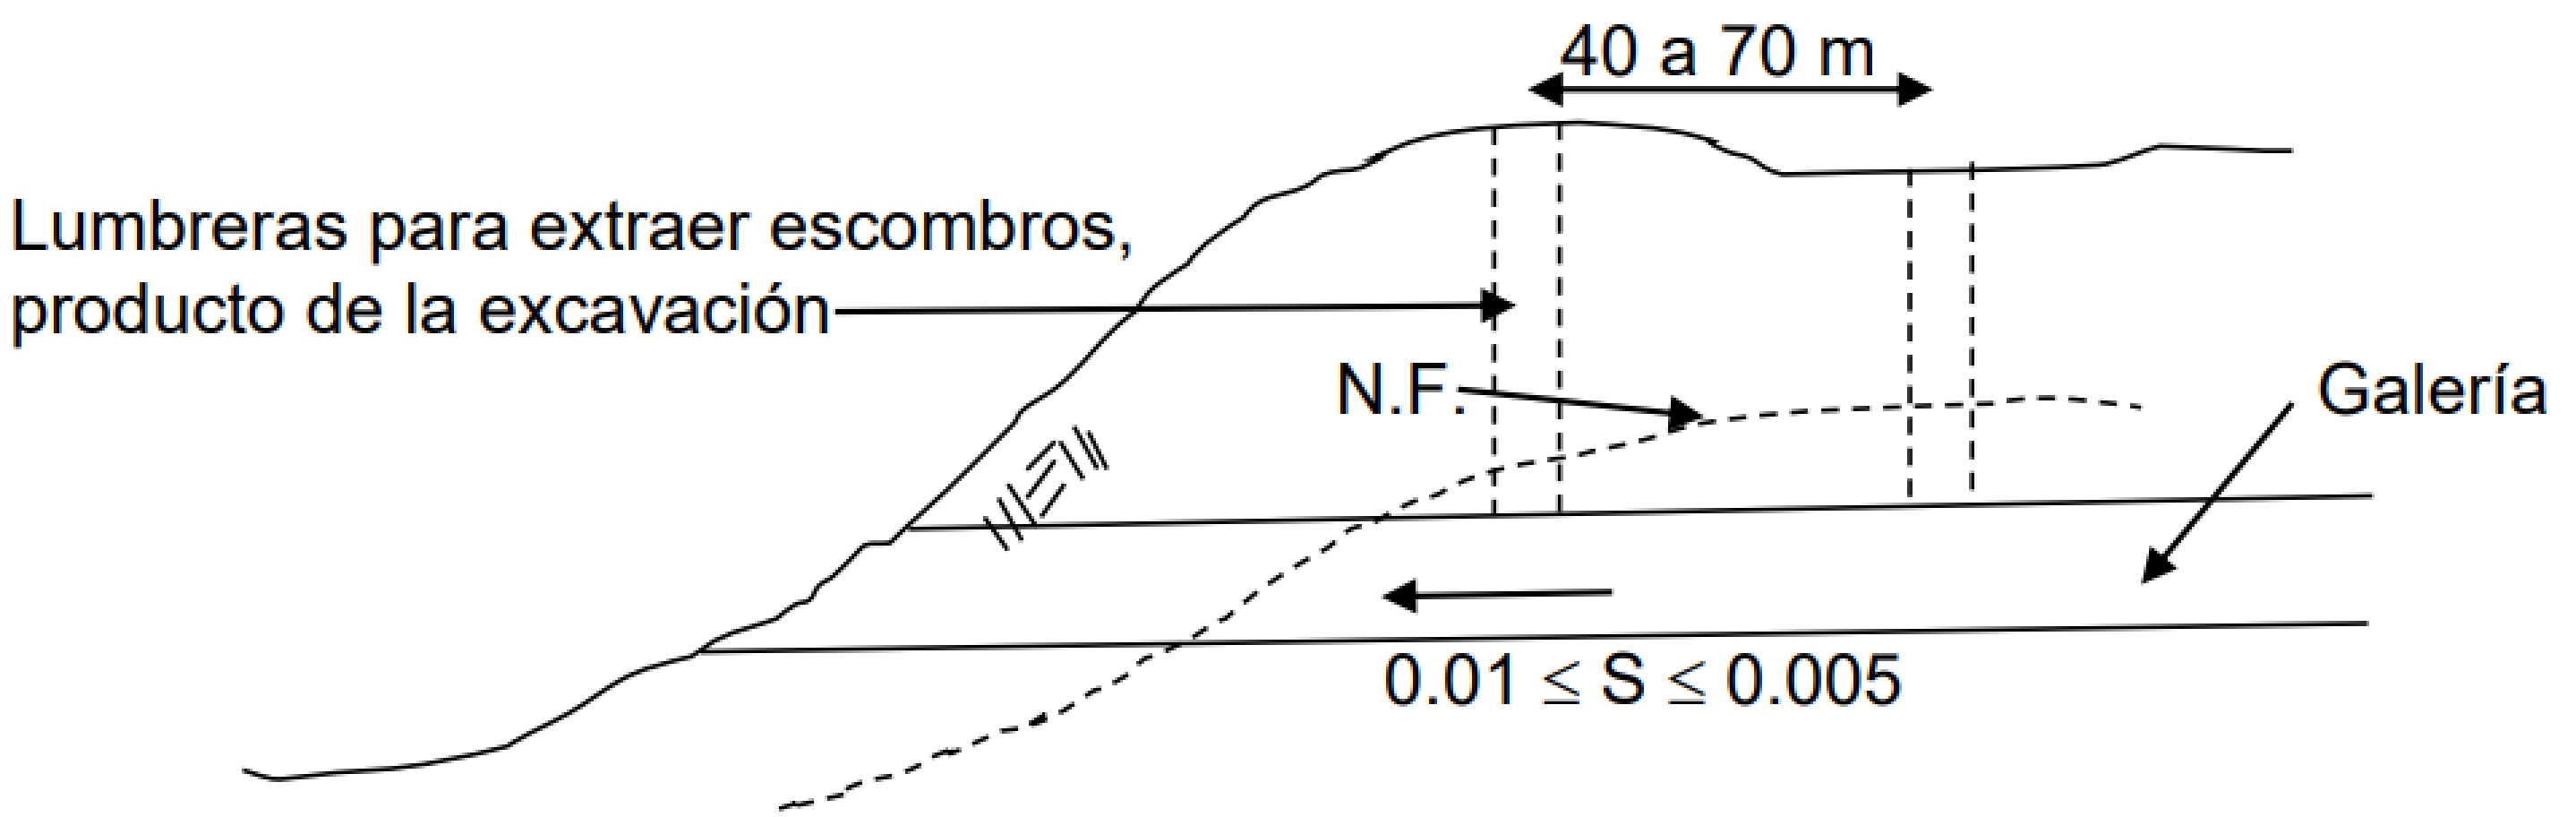
\includegraphics[width=\linewidth]{fii16.png}
		\caption{Galerías de Captación}
		\label{fii16}
	\end{subfigure}
	\begin{subfigure}[b]{0.45\linewidth}
		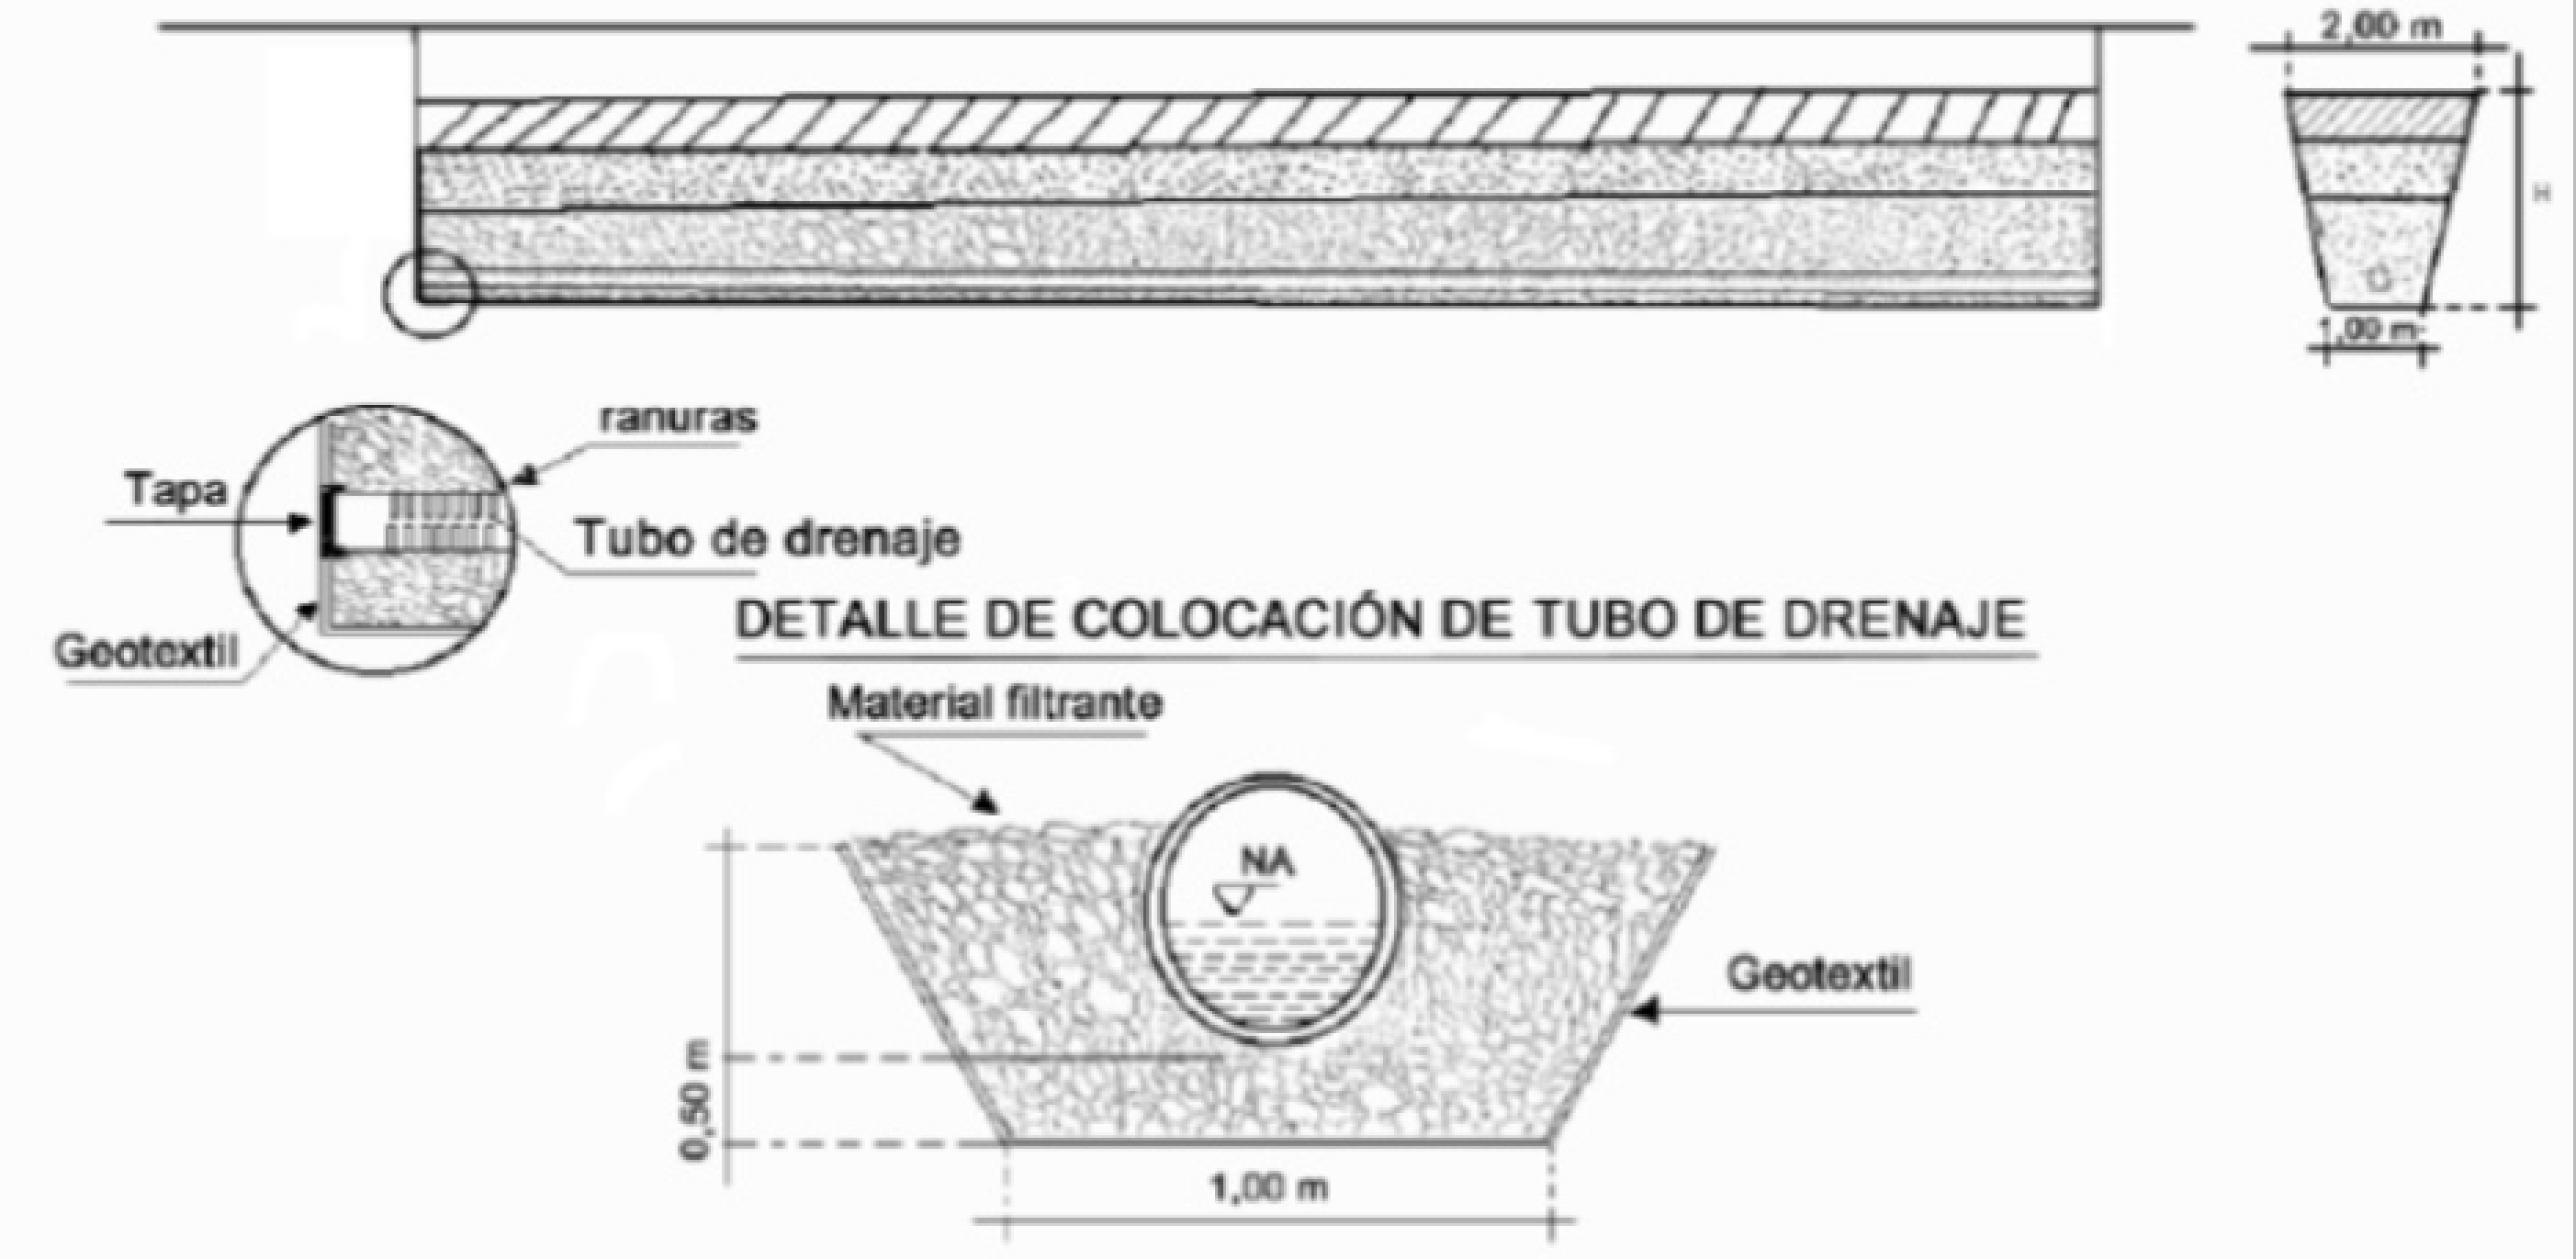
\includegraphics[width=\linewidth]{fii17.png}
		\caption{Galerías en el Fondo de Pozos}
		\label{fii17}
	\end{subfigure}
	\caption{Pozos}
	\label{fig14-17}
\end{figure}

Sí la galería es de longitud considerable, se requieren lumbreras o pozos para
extraer escombros, a distancias no mayores de 50 o 60 m.
Ventajas e inconvenientes de la explotación de Acuíferos.

Ventajas:
\begin{itemize}
	\item  Menores pérdidas por evaporación con relación a los aprovechamientos de
	      aguas superficiales
	\item Menor exposición a la contaminación
	\item Disponibilidades de agua menos afectadas por las variaciones climáticas
	\item No existe pérdida en la capacidad de almacenamiento
	\item Temperatura del agua constante.
\end{itemize}

Desventajas:
\begin{itemize}
	\item  Alto costo, tanto de construcción como de operación
	\item Aguas con riesgo de afectación salina
	\item Abatimientos acelerados de los acuíferos
	\item Para fines agrícolas, los gastos disponibles son de 20 a 65 lps (bombas entre
	      4" y 8" de diámetro en turbinas verticales)
	\item Se presentan grandes dificultades en la operación, por los pequeños gastos
\end{itemize}

Factores que afectan la explotación de las aguas subterráneas, al utilizar bombeo
\begin{itemize}
	\item Aspecto legal
	\item Rendimiento del pozo
	\item Niveles de abatimiento
	\item Éxito de empresas locales semejantes
	\item Disponibilidad de energía y/o combustibles
	\item Estudio agroeconómico y diseño ingenieril
	\item Posibilidades de recarga natural o artificial.
\end{itemize}

\subsubsection{Balance hidrológico de la cuenca}
Dependiendo del origen que se tenga del agua, según el FOGAFAGA \autocite{de1958fomento}, esta
puede ser clasificada como:

\begin{enumerate}
	\item \textbf{Agua meteórica}. Esta agua se deriva de la atmósfera, se precipita en la
	      superficie y puede penetrar en las reservas del subsuelo y regresar de nuevo a la
	      atmósfera.
	\item \textbf{Agua juvenil}. Esta es agua nueva, que de acuerdo a cuál es su origen a su vez
	      se subclasifica en: magmática, volcánica y cósmica. El agua juvenil magmática, es el
	      agua desalojada del magma durante su cristalización; el agua juvenil volcánica, es el
	      agua que proporciona los escurrimientos de lava; y el agua juvenil cósmica es el agua
	      que proviene del espacio con los meteoritos.
	\item \textbf{Agua rejuvenecida}. Es el agua que regresa o se une de nuevo al agua terrestre
	      por procesos geológicos de compactación y metamorfismo. La compactación reduce la
	      porosidad de sedimentos arcillosos desde un 50\% en material depositado
	      recientemente hasta 3 o 4\% en lutitas. Este tipo de agua rejuvenecida se puede
	      denominar aguas de compactación.
	\item \textbf{Agua connata}. Esta agua es aquella que se presenta como bolsas de agua
	      estancada, especialmente en estructuras que contienen aceite y gas.
	      Las principales reservas naturales del agua son: la atmósfera, la cual abastece a
	      todas las demás reservas; la superficie del suelo sobre la cual se encuentra el agua en
	      corrientes, lagos, océanos y agua sólida como nieve y hielo; la zona del suelo, la cual
	      actúa como reserva de humedad del suelo útil a la vida vegetal y la reserva de aguas
	      subterráneas.
\end{enumerate}

El agua es un constituyente variable de la atmósfera cuya cantidad varía con la
temperatura del aire. Grandes cantidades de vapor de agua están presentes en el aire
caliente saturado de los trópicos. El agua está limitada en la atmósfera en la zona de
convección, ese decir el estrato basal de la atmósfera de once kilómetros de espesor.
La lluvia es la fuente de toda el agua superficial y subterránea y por lo tanto debe ser
medida y analizada.

El agua superficial consta de dos cuerpos distintos de agua en la naturaleza: a)
el agua oceánica, la cual se encuentra altamente mineralizada. El cuerpo de
agua oceánica contiene agua para cubrir todo el globo terráqueo; es la principal fuente
de humedad atmosférica y por ende, de los demás cuerpos de agua. b) Los cuerpos
superficiales de agua dulce, que cubren pequeñas porciones de la superficie terrestre.
El agua dulce se halla en ríos, depósitos y lagos; es almacenada durante el invierno
como nieve o hielo.

Aún en regiones caracterizadas por abundantes cuerpos de agua superficial, la
mayoría de seres vivos, no vivirían si el agua almacenada del
suelo no fuera útil para la conservación de las plantas. Tomando como promedio 1.5 m
de espesor de la zona que penetran las raíces, la humedad contenida en el suelo es
equivalente a poco menos de 30 cm de agua. El agua almacenada en el suelo está
adherida a las partículas del mismo y es removida en gran parte por la transpiración de
las plantas. Este déficit o pérdida debe ser repuesto antes de que el agua se pueda
mover hacia abajo, hasta el espejo del agua a través de la zona vacía del suelo. Por
consiguiente, la filtración del agua de lluvia no puede ser una fuente importante del
agua en regiones áridas.

\subsubsection*{Agua para fines agrícolas.}
En forma natural, se tiene en la precipitación, la cual
para satisfacer las necesidades de la planta, se debe contar con un
temporal eficiente, de lo contrario, se recurre a
fuentes secundarias de agua, ya sea de agua superficial o de agua subterránea.
En México, como se señaló en la sección \ref{subsubciclohidro}, se tiene una precipitación promedio
de 780 mm. El escurrimiento superficial se estima del orden del 27\% de la
precipitación, haciendo un total de 410,000 millones de $ m^3$ como escurrimiento virgen, y
357,565 millones de $ m^3$ como escurrimiento disponible para aprovecharse, con una
distribución un tanto similar a como se presenta la precipitación. véase la figura \ref{fii8}.

Por su naturaleza, la cuantificación del agua subterránea permite identificar:
31,000 millones de $m^3$ de agua subterránea renovable anualmente y 110,000 millones
de $ m^3$ de agua subterránea no renovable.

\begin{figure}[h!]
	\centerline{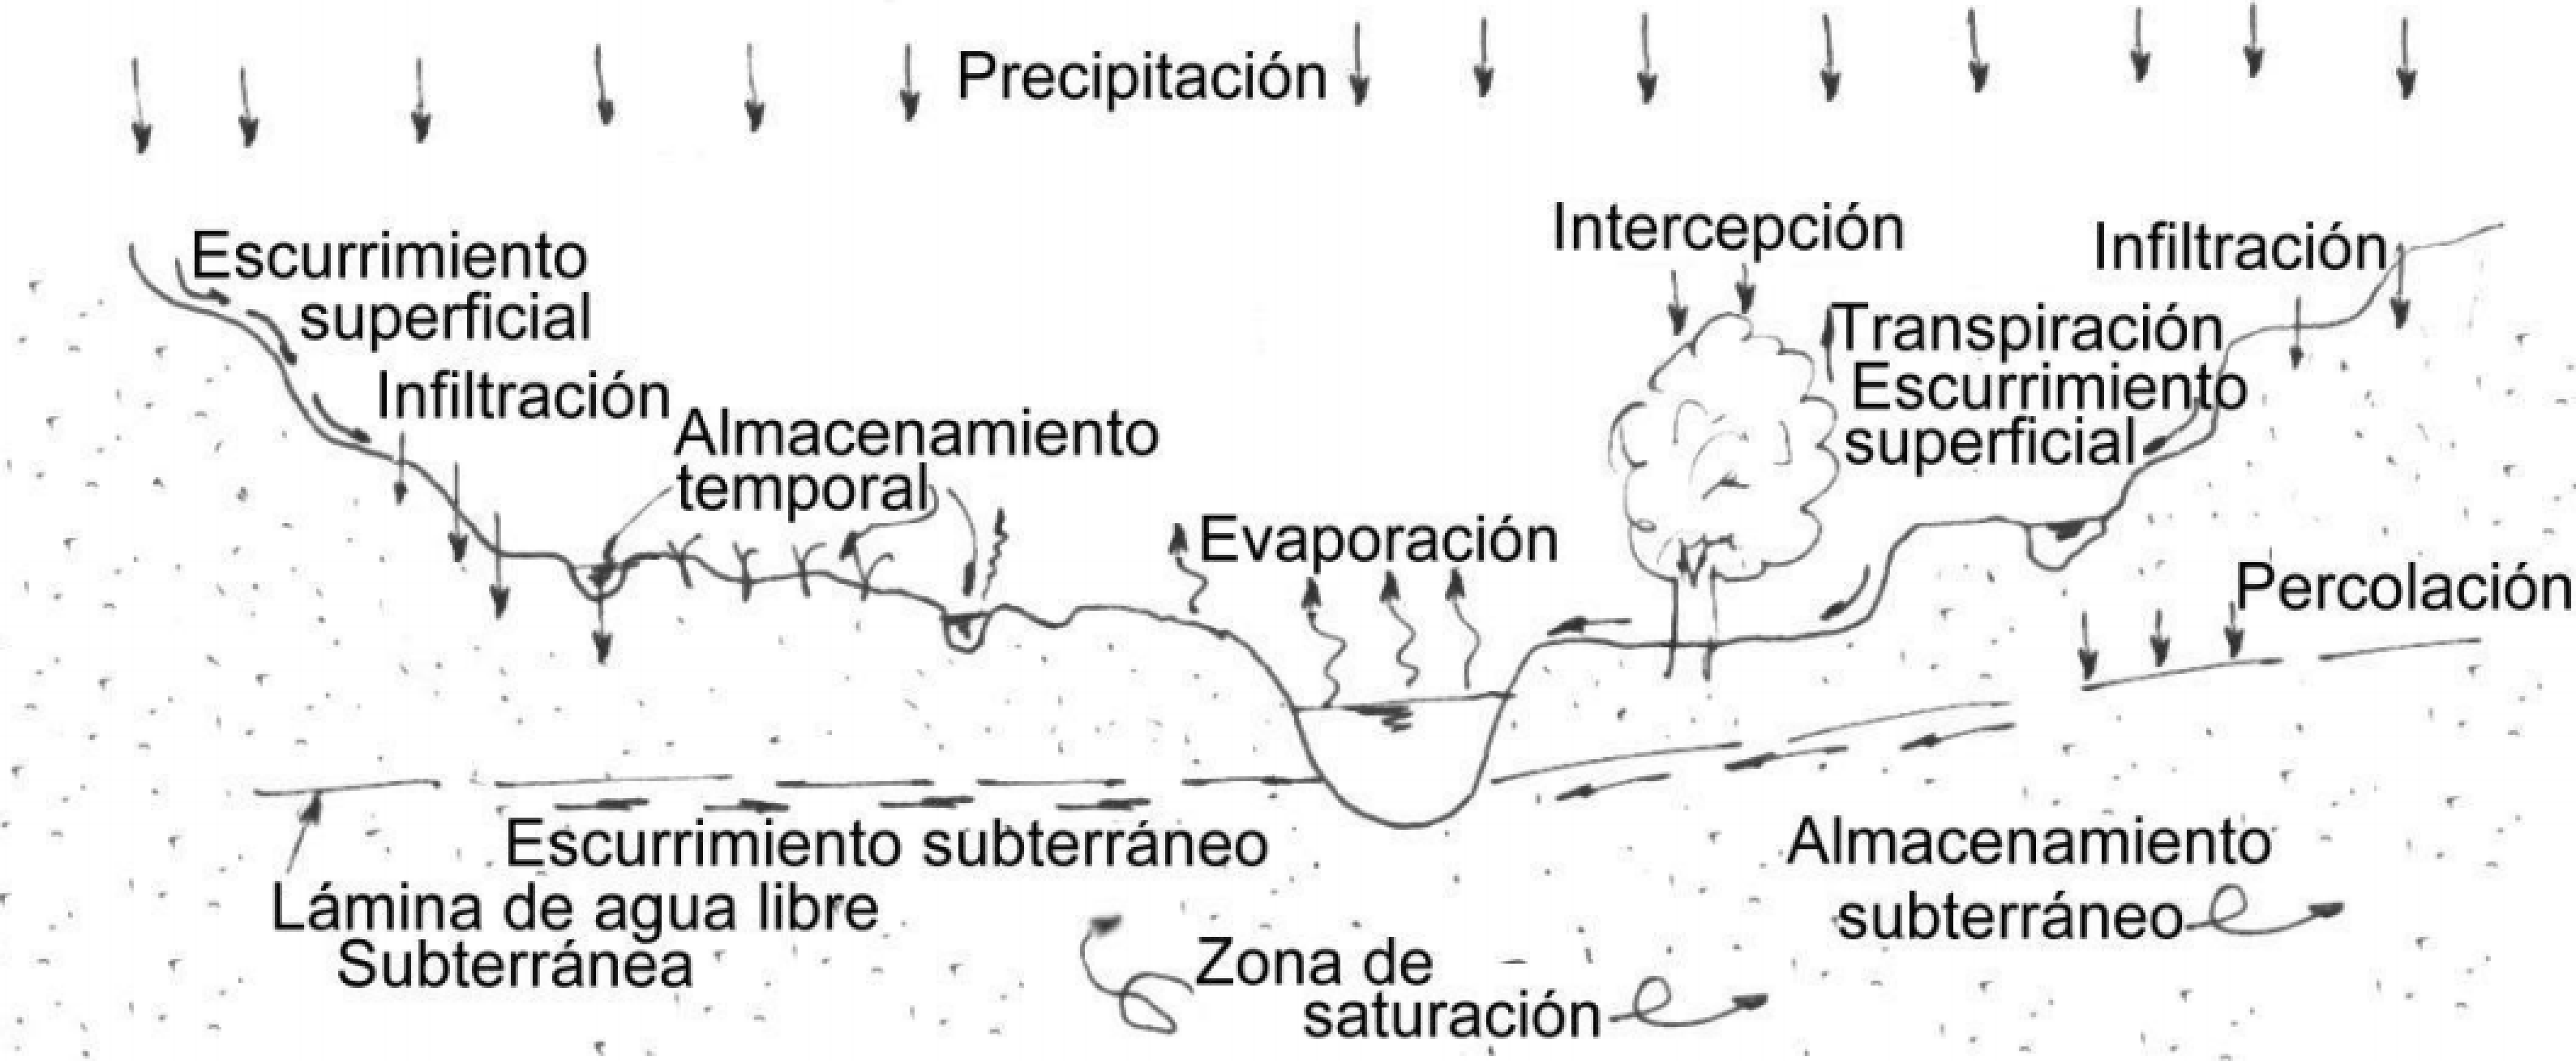
\includegraphics[width=0.7\textwidth]{fii18.png}}
	\caption{Disposición de la humedad durante una lluvia intensa (según Houk)}
	\label{fii18}
\end{figure}

\subsubsection{Ciclo del agua}
Las principales fuentes de energía para la circulación del agua en la naturaleza
son: el sol y la gravedad.
\begin{definition}[Evaporación]
	Según su definición hidrológica es la tasa neta de
	transporte de vapor hacia la atmósfera.
	La tasa de evaporación varía según la naturaleza de la superficie evaporante y
	de diversos factores meteorológicos. En la primera, están todas las superficies
	expuestas a la precipitación tales como vegetales, edificios, calles pavimentadas, que
	vienen a representar superficies potenciales de evaporación; entre los segundos se
	tiene como principal factor a la radiación y en forma secundaria, a la velocidad del
	viento y la presión de vapor de la capa de aire inmediatamente superior.
\end{definition}

\begin{definition}[Precipitación]
	Es el agua que llega a la superficie terrestre proveniente de la
	atmósfera. Este es un componente fundamental del ciclo hidrológico.
	Las formas de precipitación, se tienen dependiendo de las condiciones
	meteorológicas existentes, pudiendo ser:
\end{definition}
\begin{itemize}
	\item \textbf{llovizna}: gotas de agua con diámetro
	      menor de 0.5 mm y su intensidad es generalmente de 1.0mm/h por lo cual semejan
	      estar flotando en el aire y por ello siguen con facilidad el curso del viento
	\item \textbf{Lluvia}: son
	      gotas de agua que caen de las nubes con un diámetro superior a 0.5 mm y a
	      velocidades que varían de acuerdo a su intensidad y puede a su vez dividirse en lluvia
	      ligera (2.5 mm), mediana o moderada (2.5 a 7.5 mm) o intensa o fuerte (diámetros de
	      7.5 mm), si la lluvia y llovizna se presentan cuando la temperatura ambiente es menor a
	      0$^{\circ}$C entonces se forma una capa de hielo en las superficie en que caen
\end{itemize}

\begin{definition}[Granizo]
	Está constituido por bolas o pedriscos de hielo de 5 a 50 mm que son producto de la
	condensación de gotas de lluvia formando granos de hielo duro, poco transparente y de
	forma globular, que caen separados o en grupos irregulares
\end{definition}

\begin{definition}[Nieve]
	La constituyen
	cristales de hielo de color blanco, traslucido ramificado, generalmente en forma de
	estrellas hexagonales (vistos al microscopio). Atendiendo a su intensidad, esta puede
	ser ligera, moderada y fuerte y la nieve puede observarse sola o acompañada de algún
	otro fenómeno que disminuye la visibilidad.
\end{definition}

\begin{definition}[Rocío]
	Es el vapor de agua que se
	condensa sobre la superficie a causa de que el aire ambiente sufre un descenso de
	temperatura, este descenso nunca es inferior a 0$^{\circ}$C
\end{definition}

\begin{definition}[Escarcha]
	Es debida a un
	fenómeno llamado de sublimación, por el cual los cristales de hielo son formados
	directamente sobre las superficies, en virtud de que el aire se ha enfriado a menos de
	0$^{\circ}$C.
\end{definition}

La precipitación puede ser: \textbf{convectiva}, \textbf{ciclónica} u \textbf{orográfica}.

\begin{definition}[Precipitación convectiva]
	Se origina por el calentamiento del suelo, que
	provoca corrientes ascendentes de aire húmedo. La precipitación asociada a este tipo
	de fenómeno afecta áreas reducidas, del orden de 25 a 50 $Km^2 $, y su intensidad varía
	entre lloviznas ligeras y aguaceros, dependiendo de las condiciones de temperatura y
	humedad.
\end{definition}

\begin{definition}[precipitación ciclónica]
	Está asociada al paso de ciclones, resulta del
	levantamiento de aire por convergencia de la masa de aire en una zona de baja
	presión. En general afectan zonas extensas. Se divide en dos tipos: frontal y por
	convergencia.
\end{definition}

\begin{definition}[Precipitación ciclónica frontal]
	Puede ser de frente caliente o de frente frío,
	siendo originada por el levantamiento de aire caliente sobre el frío, y puede ocurrir
	cuando el aire caliente se mueve hacia el frío (frente caliente) o viceversa (frente frío).
	La precipitación provocada por un frente caliente se distribuye sobre un área bastante
	grande y varía entre intensidades ligeras y moderadas. La precipitación de frente frío es
	de intensidades fuertes y de corta duración.
\end{definition}

\begin{definition}[Precipitación ciclónica por convergencia]
	Es causada por la tendencia del aire
	húmedo a converger hacia el centro del ciclón. El aire al no poder concentrarse en un
	área menor tiende a elevarse, por lo cual se enfría provocando la precipitación.
	La precipitación orográfica es consecuencia del ascenso del aire producido por
	las barreras montañosas; su distribución en el espacio está relacionada con las
	pendientes del terreno.
\end{definition}

En terrenos demasiado abruptos, la influencia orográfica es muy
señalada, por lo que la distribución espacial de las lluvias tiende a parecerse de una
tormenta a otra. Cuando no está relacionada con acciones ciclónicas o convectivas,
resulta ser de baja intensidad tal como se muestra en la figura \ref{fii19}.

\begin{figure}[h!]
	\centerline{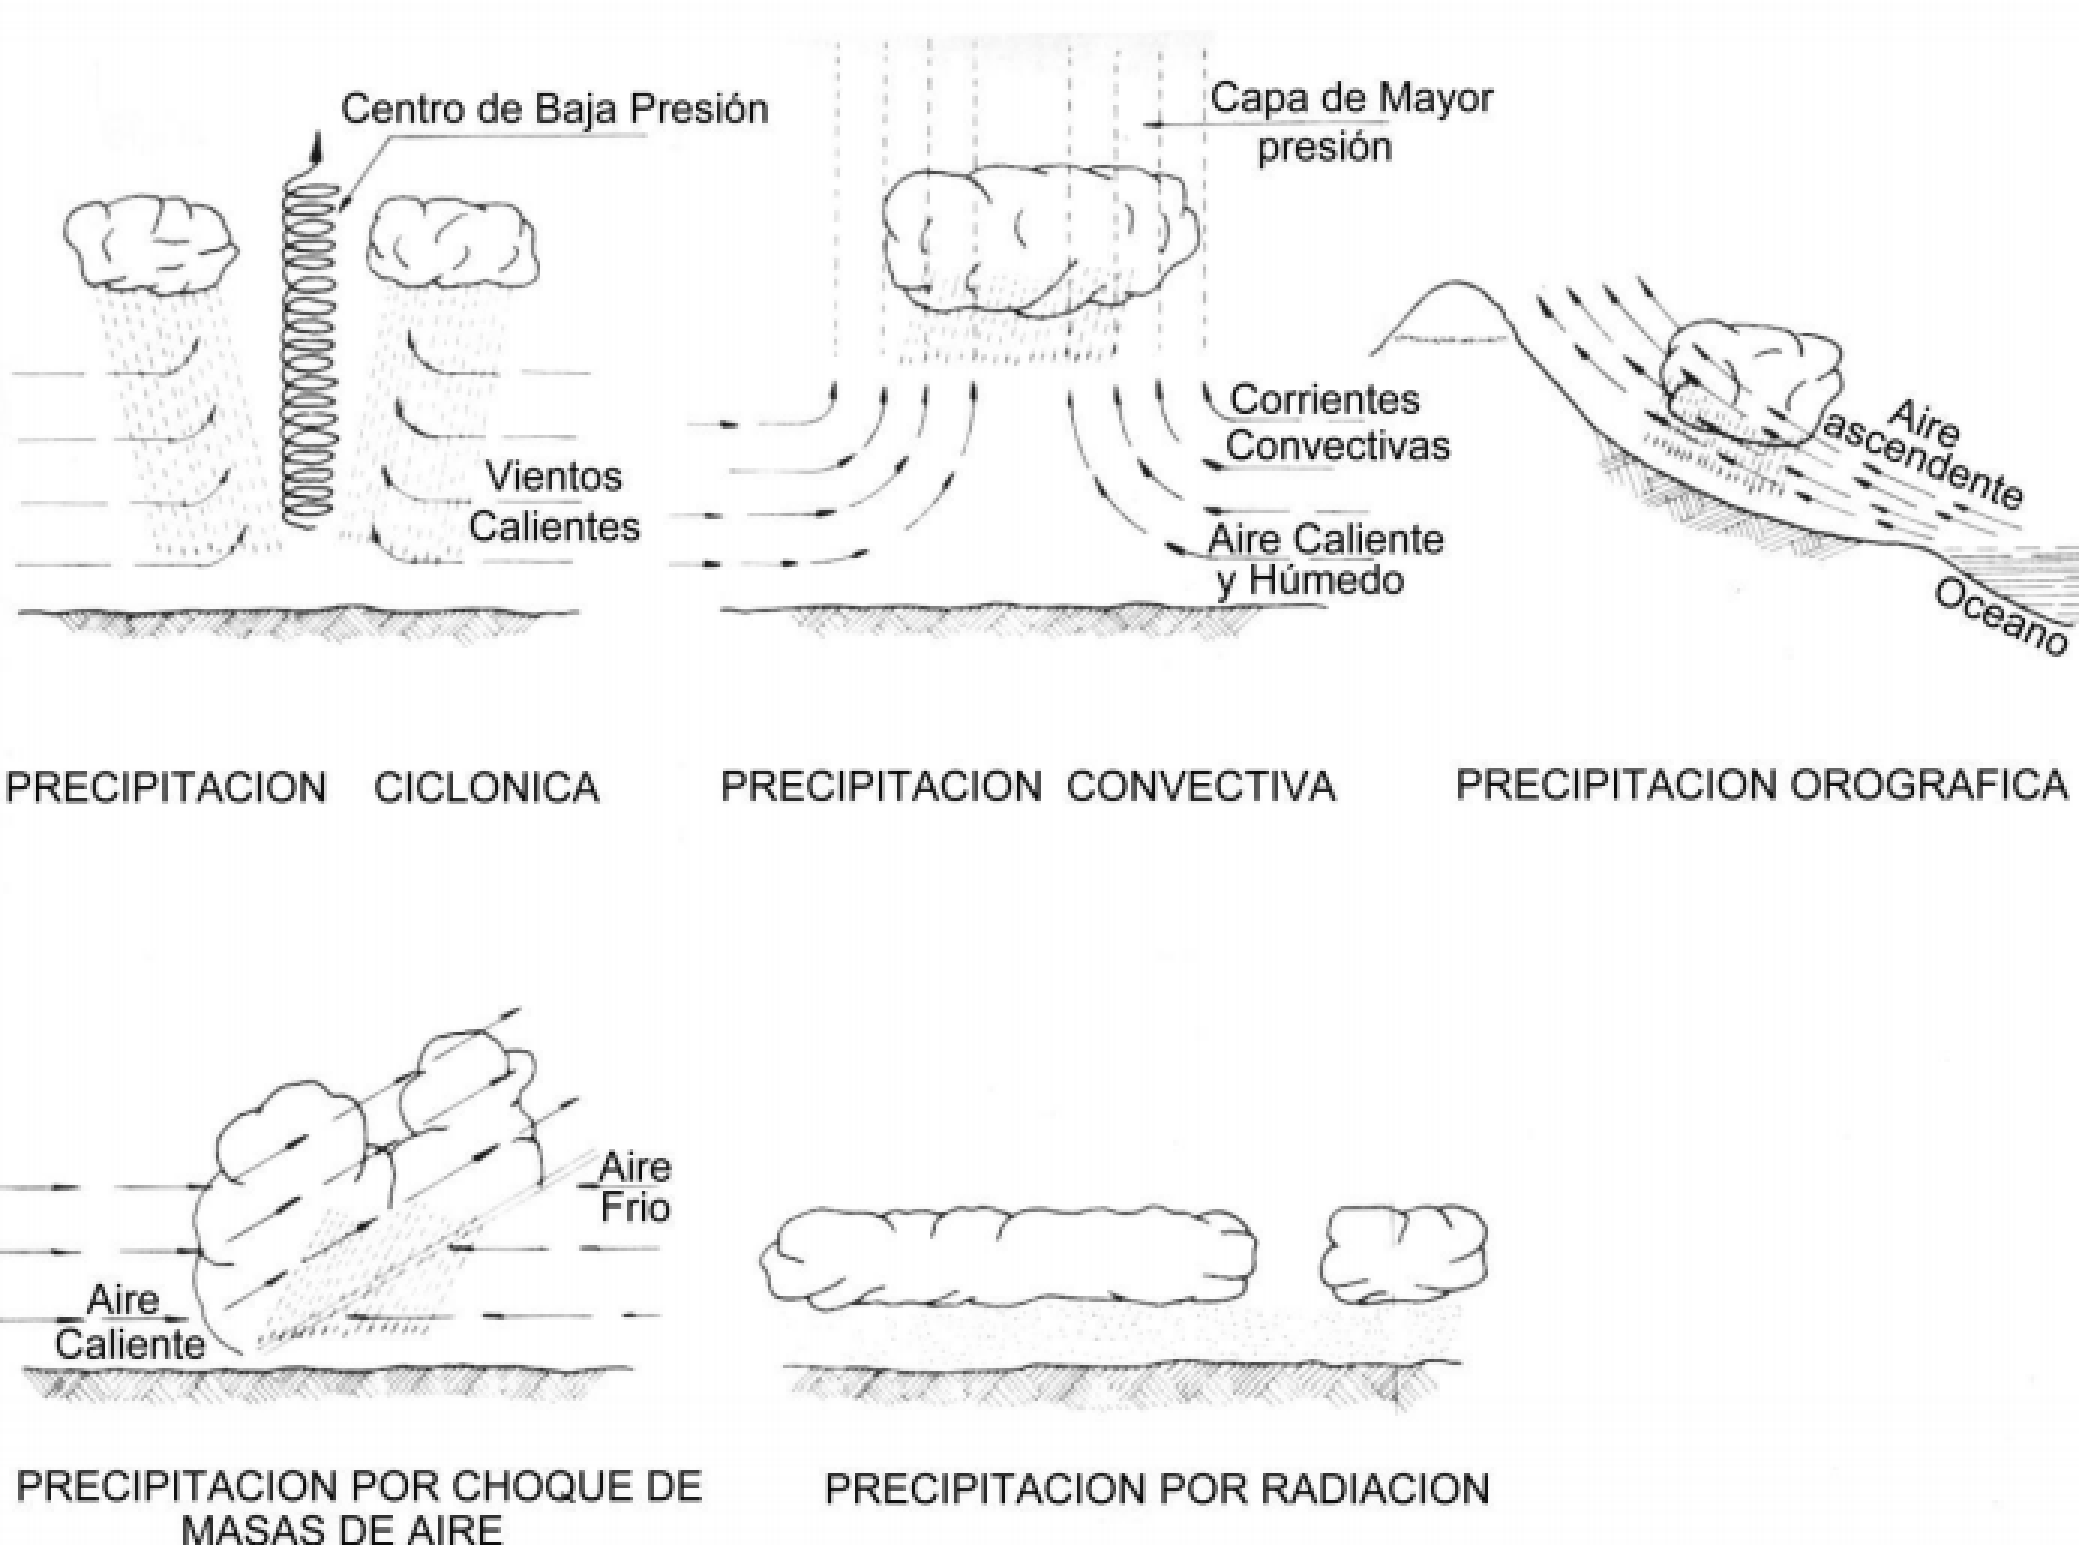
\includegraphics[width=0.7\textwidth]{fii19.png}}
	\caption{Esquemas de los tipos de precipitación}
	\label{fii19}
\end{figure}

\subsubsection{Distribución de la precipitación.}

\textbf{Infiltración}. Es el movimiento vertical del agua, a través de las capas
superficiales del suelo, producido por la acción de las fuerzas gravitacionales y
capilares.

Esta es la porción más considerable de las pérdidas de la precipitación. Existen
diferentes métodos para calcular la infiltración, entre las que se pueden citar la de
Horton y la de Kostiakov.

\textbf{Evaporación}. Existe otra porción de la precipitación que se pierde cuando
va cayendo y esta es la evaporación que se tiene cuando caen las gotas de agua.

\textbf{Transpiración}. Es el agua que se despide en forma de vapor de las hojas
de las plantas. Esta agua es tomada por las plantas en forma natural del suelo.

\textbf{Almacenamiento temporal}. En las depresiones del terreno, se presenta
una retención por determinado tiempo de cierta cantidad de agua, la que después parte
se infiltra y parte se evapora.

\textbf{Escurrimiento}. Es el agua proveniente de la precipitación que circula
sobre o bajo la capa superficial del suelo o en estratos más profundos y que llega a una
corriente para finalmente ser drenada hasta la salida de una cuenca. Existen tres tipos
de escurrimiento: superficial, subsuperficial y subterráneo.

La relación entre el volumen escurrido y el volumen precipitado en una
determinada cuenca es lo que origina el concepto de \textbf{coeficiente de escurrimiento} $(Ce)$,
fundamental para determinar el primero conociendo el segundo, variando entre valores
que van de $0.1$ a $0.25$.

\subsubsection{Los consejos de cuenca}
Los Consejos de Cuenca son instancias de coordinación y concertación entre la
Comisión Nacional del Agua, las dependencias y entidades de las instancias federal, estatal,
municipal y los representantes de los usuarios de la respectiva cuenca hidrológica: Su objeto es
formular y ejecutar programas y acciones para la mejor administración de las aguas, el
desarrollo de la infraestructura hidráulica y de los servicios respectivos y la preservación de los
recursos de la cuenca (Art. 13, LAN).

Para su funcionamiento, los Consejos de Cuenca pueden contar con organizaciones
auxiliares a nivel de subcuenca, microcuenca y/o acuífero, denominadas respectivamente:
Comisiones de Cuenca, Comités de Cuenca y Comités Técnicos de Aguas Subterráneas
(Cotas).

%imágen aquí vaaaaaaaaaaaaaaaaaaaaaaaaaaa

Al año 2000, se tenían instalados 25 consejos de cuenca, así mismo al año 2003
se tenían instaladas 11 comisiones de cuenca y al año 2004, 16 comités de cuenca y
69 Comités Técnicos de Aguas Subterráneas (COTAS).

\subsection{Ley de Aguas Nacionales.}

La ley de aguas nacionales es reglamentaria de artículo 27 de la Constitución
política de los Estados Unidos Mexicanos es de observancia general en todo el territorio
nacional, sus disposiciones son de orden público e interés social y tiene por objeto
regular la explotación, uso o aprovechamiento de dichas aguas, su distribución y
control, así como la preservación de su cantidad y calidad para lograr su desarrollo
integral sustentable.

Se conforma con 10 títulos, el título primero de \textbf{disposiciones generales} contiene
un solo capítulo y 3 artículos.

El Título Segundo, de la \textbf{Administración del agua}, contiene 10 capítulos y 11
artículos base y 20 sub articulos.

El Título Tercero, de la \textbf{política y programación hídrica}, contiene un solo capítulo,
pero dos secciones, un artículo y tres sub artículos.

El Título Cuarto, de los \textbf{Derechos de Explotación, Uso o Aprovechamiento de
	Aguas Nacionales}, contiene cinco capítulos y dos subcapítulos, 10 artículos y 8
sub artículos.

El Título Quinto, de las \textbf{Zonas Reglamentadas, de Veda o de Reserva}, contiene
un solo Capítulo, seis artículos y un subartículo.

El Título Sexto, de los \textbf{Usos del Agua}, con cinco capítulos y dos subcapítulos, el
capítulo dos tiene cinco secciones, y todos comprenden 41 artículos y siete
sub artículos.

El Título Séptimo, de la \textbf{Prevención y Control de la Contaminación de las Aguas y
	Responsabilidad por Daño Ambiental}, con dos capítulos, con 13 artículo y 10
sub artículos.

El Título Octavo, de la \textbf{Inversión en Infraestructura Hidráulica}, contiene cuatro
capítulos, 15 artículos y 3 sub artículos.

El Titulo Noveno, de los \textbf{Bienes Nacionales a Cargo de ``la Comisión''}, contiene
un solo capítulo, y 5 artículos y 4 sub artículos.

El Titulo Decimo, de las \textbf{Medidas de Apremio, Seguridad, Infracciones, Sanciones
	y Recursos}, contiene tres capítulos, 6 artículos y 6 sub artículos.

La anterior Ley es del año 1992, pero en el año 2003 se actualizó con 16
transitorios, en el año 2004, con un artículo, en el 2008 con un Transitorio, en el año
2011 se reforman y adicionan los artículos 7 Bis y 18 de la Ley, en el año 2011 con un
transitorio, en el año 2012 con un artículo y un transitorio.

Para poder implementar cualquier ley, se requiere del Reglamento, así el
Reglamento de la ley de Aguas Nacionales, el cual se conforma con 11 títulos:

El Título primero de las Disposiciones Preliminares, contiene un solo capítulo,
con 5 artículos.

El Título Segundo, de la Administración del Agua, contiene cuatro capítulos, con
15 artículos.

El Título Tercero, de la Programación Hidráulica, contiene un solo capítulo, con
seis artículos.

El Título Cuarto, de los Derechos de Uso o Aprovechamientos de Aguas
Nacionales, contiene cinco capítulos, con 44 artículos.

El Título Quinto, de las Zonas Reglamentadas, de Veda o de Reserva, contiene
un solo capítulo, con 8 artículos.

El Título Sexto, de los Usos del Agua, contiene cinco capítulos, el segundo
Capítulo tiene cinco secciones, que es el que se refiere al Uso Agrícola, y las secciones
son: la primera de Disposiciones generales, la segunda de Ejidos y comunidades, la
tercera de las Unidades de riego, la cuarta de los Distritos de Riego y la Quinta del
Drenaje Agrícola, todo el Título conforma 52 artículos.

El Título Séptimo, de la Prevención y Control de la Contaminación de las Aguas,
solo contiene un Capítulo, con 24 artículos.

El Titulo Octavo, de la Inversión en Infraestructura Hidráulica, contiene dos
capítulos, con 10 artículos.

El Titulo Noveno, de los Bienes Nacionales a Cargo de la Comisión, contiene un
solo capítulo, con 15 artículos.

El Titulo Décimo, de las Infracciones, Sanciones y Recursos, contiene tres
capítulos, con 16 artículos.

El Título Décimo Primero, de la Conciliación y Arbitraje, contiene un solo capítulo,
con cinco artículos.

El reglamento concluye con 14 Transitorios, para el año 1994. En el año 1997, se
reformó la ley de Aguas Nacionales con un solo artículo y dos transitorios; en el año
2002, se reforma el Artículo 13 del Reglamento, con un solo artículo y un transitorio.

\subsection{Cambio climático}
El estudio del clima es un campo de investigación complejo y en rápida evolución,
debido a la gran cantidad de factore que intervienen. El clima de la Tierra nunca ha
sido estático. Como consecuencia de alteraciones en el balance energético, está
sometido a variaciones en todas las escalas temporales, desde decenios a miles y
millones de años. Entre las variaciones climáticas más destacables que se han
producido a lo largo de la historia de la Tierra, figura el ciclo de unos 100,000 años, de
períodos glaciares, seguido de períodos interglaciares.

\begin{definition}[Cambio climático]
	Es la variación global del clima de la Tierra. Es debido
	a causas naturales y también a la acción del hombre y se producen a muy diversas
	escalas de tiempo y sobre todos los parámetros climáticos: temperatura,
	precipitaciones, nubosidad, etc$\dots$
\end{definition}

\begin{definition}[Efecto invernadero]
	Se refiere a la retención del calor del Sol en la atmósfera de la Tierra por parte de una capa de gases
	en la atmósfera. Sin ellos la vida, tal como la conocemos, no sería posible, ya que el
	planeta sería demasiado frío. Entre estos gases se encuentran el dióxido de carbono,
	el óxido nitroso y el metano, que son liberados por la industria, la agricultura y la
	combustión de combustibles fósiles. El mundo industrializado ha conseguido que la concentración de estos gases haya aumentado un 30\% desde el siglo pasado, cuando,
	sin la actuación humana, la naturaleza se encargaba de equilibrar las emisiones.
\end{definition}

Ya en el año 2001 el Tercer Informe de Evaluación del Grupo Intergubernamental
de Expertos sobre Cambio Climático \textbf{(IPCC)} ponía de manifiesto la evidencia
proporcionada por las observaciones de los sistemas físicos y biológicos que mostraba
que los cambios regionales en el clima, en concreto los aumentos de las temperaturas,
estaban afectando a los diferentes sistemas y en distintas partes del globo terráqueo.
Señalaba, en definitiva, que se están acumulando numerosas evidencias de la
existencia del cambio climático y de los impactos que de él se derivan. En promedio, la
temperatura ha aumentado aproximadamente $0{.}6^\circ C$ en el siglo XX. El nivel del mar ha
crecido de 10 a 12 centímetros y los investigadores consideran que esto se debe a la
expansión de océanos, cada vez más calientes.

El cambio climático nos afecta a todos. El impacto potencial es enorme, con
predicciones de falta de agua potable, grandes cambios en las condiciones para la
producción de alimentos y un aumento en los índices de mortalidad debido a
inundaciones, tormentas, sequías y olas de calor. En definitiva, el cambio climático no
es un fenómeno sólo ambiental sino de profundas consecuencias económicas y
sociales. Los países más pobres, que están peor preparados para enfrentar cambios
rápidos, serán los que sufrirán las peores consecuencias.

Se predice la extinción de animales y plantas, ya que los hábitats cambiarán tan
rápido que muchas especies no se podrán adaptar a tiempo. La Organización Mundial
de la Salud ha advertido que la salud de millones de personas podría verse amenazada
por el aumento de la malaria, la desnutrición y las enfermedades transmitidas por el
agua.

En consecuencia, aunque existen incertidumbres que no permiten cuantificar con
la suficiente precisión los cambios del clima previstos, la información validada hasta
ahora es suficiente para tomar medidas de forma inmediata, de acuerdo al denominado
``principio de precaución'' al que hace referencia el Artículo 3 de la Convención Marco
sobre Cambio Climático. La inercia, los retrasos y la irreversibilidad del sistema
climático son factores muy importantes a tener en cuenta y, cuanto más se tarde en
tomar esas medidas, los efectos del incremento de las concentraciones de los gases de
efecto invernadero serán menos reversibles.

\subsubsection{Consecuencias del cambio climático}
El cambio climático, desde la existencia de la tierra no solo ha permitido
modificar las condiciones de la naturaleza, sino que también va haciendo variaciones
en la economía; en la salud y en todas las poblaciones de una u otra manera.

No obstante, se ha determinado científicamente que el cambio climático va
llegando a su límite y al no ponerle un freno definitivo a estos aspectos en este, que es
el tiempo oportuno; las consecuencias que se pueden afianzar son devastadoras y se
garantiza que los resultados terminen completamente en desastres.

Las consecuencias comprobadas que se identifican con el cambio
climático son:

\begin{enumerate}
	\item El agua se expande al percibir el intenso calor; dado que son los océanos los
	      que absorben más calor que la tierra firme. De este modo, el nivel del mar
	      aumenta.
	\item Gracias a la fusión de los glaciares y el hielo marino como consecuencia del
	      calor excesivo; el nivel del mar también se ve aumentado desde esta
	      perspectiva.
	\item Como consecuencia al aumento del nivel del mar, se presentan las inundaciones
	      de todas las poblaciones aledañas.
	\item Sitios en los que llueve o nieva en condiciones normales, puede llegar a
	      calentarse y con ello, secarse por completo, al igual los lagos y los ríos.
	\item Al disminuir las zonas de lluvia, va provocando la deforestación y
	      posterior desertificación del suelo.
	\item Se presentarían condiciones de fuerte sequía, manteniendo el riesgo de pérdida
	      para los cultivos
	\item El agua para agricultura; producción de comida, bebida o uso general estaría
	      limitado por las condiciones atmosféricas.
	\item Comenzaría la crítica extinción de muchas especies animales y de vegetación,
	      por falta de agua para su nutrición.
	\item Huracanes, tornados, terremotos y tormentas provocadas por las variaciones
	      de temperatura que el planeta va ejerciendo drásticamente y de forma descontrolada, conllevando al mismo tiempo a la evaporación del agua que
	      tendría efecto con mucha más regularidad de lo normal.
\end{enumerate}

\subsubsection{Soluciones}

Las distintas soluciones aptas e indicadas para disminuir la frecuencia entre
los cambios del clima que vive la Tierra se basan en medidas ejercidas directamente
por la actividad humana, con el fin de contrarrestar las acciones dadas directamente por
la naturaleza y por los factores energéticos que son inevitables.

Por ello, la educación es la base para mejorar las condiciones y la \textbf{protección del
	medio ambiente}, teniendo en cuenta varios métodos óptimos cuando se trata de
disminuir el cambio climático, los cuales son:

\begin{enumerate}
	\item \textbf{Reciclar:} Reciclar es el comienzo para volver a restituir la vida del planeta, evitando el
	      empeoramiento del cambio climático. Al reciclar \textbf{1 Kg} de latas de aluminio usadas,
	      esto consume menos energía que su producción.
	\item \textbf{Agua:} Cuando vayas a preparar alguna bebida caliente, hierve sólo el agua que
	      vayas a utilizar, igualmente dale preferencia a ducharte, no solo para ahorrar la
	      cantidad de agua sino que ahorras energía que se utiliza al calentarla.
	\item \textbf{Luces artificiales:} Cuando no estés en casa o vayas a dormir, apaga las luces, se estima que las
	      viviendas son responsables en alrededor del 30\% del consumo eléctrico que interfiere
	      con la calidad del ambiente. De esta forma no solo ahorraremos electricidad, sino
	      también colaboraremos con el cuidado del planeta.
	\item \textbf{Electrodomésticos:} No dejes a los equipos electrodomésticos en StandBy, pues por lo general
	      el 40\% de la energía que consumen algunos de ellos como los televisores lo hacen de
	      de este modo; aumentando el consumo de energía y el desgaste del medio ambiente.
	      Lo mismo sucede con los cargadores del móvil, si los dejas enchufados, gran parte de
	      la electricidad se pierde y solo el 5\% llega a utilizarse. Desenchufalo apenas lo termines
	      de usar.
	\item \textbf{Disminuye el uso de la calefacción:} Al colocar la calefacción en muy altas temperaturas; la repercusión sobre el
	      El cambio climático se intensifica debido al aumento de calor que llega a la atmósfera. Lo
	      ideal es bajar la temperatura 1$^{\circ}$C más y así poder reducir aún más la factura de la
	      energía y a la vez ayudas a la vida del planeta reduciendo las probabilidades de sus
	      consecuencias.
	\item \textbf{Alternativas al auto:} Los automóviles están identificados como los responsables del 10\% de dióxido
	      de carbono que emana hacia la atmósfera, por lo cual es una gran idea que de vez en cuando recurras al transporte público; la bicicleta o andar a pie, de forma de contribuir
	      con la reducción de los cambios de clima y el calentamiento global.
	\item \textbf{Planta un árbol:} Esta es la regla fundamental e inolvidable de todas aquellas personas que
	      quieren contribuir con el planeta y con la salud ecológica. Busca un amplio parque
	      donde sepas que tu árbol estará a salvo y planta la semilla. Esta es una estrategia de
	      mucha ayuda para el ambiente, dado que 5 árboles llegan a absorber hasta 1 tonelada
	      de dióxido de carbono en toda su vida.
	\item \textbf{Evita los combustibles fósiles:} Evita en lo máximo posible los combustibles fósiles; para así disminuir la
	      cobertura de dióxido de carbono en la atmósfera, que termina volviendo a nosotros en
	      forma de lluvia ácida. En lugar de estos, se pueden emplear alternativas al uso de
	      petróleo, gas y carbón.
	\item \textbf{Infraestructuras ecológicas:} En las medidas futuristas se recomienda adaptar las infraestructuras domiciliarias
	      como casas y edificios para aprovechar la energía y no malgastarla. Para ello se debe
	      omitir el cemento en su construcción para así evitar la emisión de gases que van
	      directo al efecto invernadero, causante y agravante del calentamiento global.
\end{enumerate}

Estos son los cuidados del medio ambiente que ayudarán a que el cambio
climático tenga una mínima progresión; ya que colaborará con la reducción de gases
en la atmósfera emitidos ante el efecto invernadero, los cuales harán que se disminuya
el uso de todos los recursos naturales; además de permitir que se ralenticen las
consecuencias dadas por el cambio de clima, provenientes directamente del
calentamiento global.

\subsection{Impacto ambiental}

El impacto ambiental es el efecto que produce la actividad humana sobre el
medio ambiente. El concepto puede extenderse a los efectos de un fenómeno natural
catastrófico. Técnicamente, es la alteración en la línea de base ambiental.

La ecología es la ciencia que se encarga de medir este impacto y tratar de minimizarlo.
Las acciones de las personas sobre el medio ambiente siempre provocarán
efectos colaterales sobre éste. La preocupación por los impactos ambientales abarca
varios tipos de acciones, como la contaminación de los mares con petróleo, los
desechos de la energía radioactiva o desechos radioactivos/nucleares, la
contaminación auditiva, la emisión de gases nocivos, o la pérdida de superficie de
hábitats naturales, entre otros.

La evaluación de impacto ambiental \textbf{(EIA)} es un procedimiento por el que se
identifican y evalúan los efectos de ciertos proyectos sobre el medio físico y social.

La Declaración de Impacto Ambiental \textbf{(DIA)} es el documento oficial que emite el órgano
ambiental al final del procedimiento de EIA, que resume los principales puntos del
mismo y concede o deniega la aprobación del proyecto desde el punto de vista
ambiental. La identificación y mitigación de impactos ambientales es el principal objetivo
del procedimiento de Evaluación de Impacto Ambiental. La aplicación de acciones de
mitigación, siguiendo la denominada "jerarquía de mitigación", pretende contrarrestar
los efectos negativos de los proyectos sobre el medio ambiente

\subsubsection{Tipos de impacto ambiental}

La preocupación por los efectos ambientalmente negativos de las acciones
humanas surgió en el marco del movimiento conservacionista, en cuyo origen está la
preocupación por la naturaleza. Esta preocupación se suma a la ya existente por la
salud y el bienestar humano, todos afectados por el desarrollo económico y urbano.
Esta dimensión es llamada medio social. Se le considera impacto cuando hay al menos
tres tipos de contaminación que son la contaminación del agua, del aire y del suelo.

\subsubsection{Impacto ambiental a nivel mundial}
La mayor parte de la energía utilizada en los diferentes países proviene
del petróleo y del gas natural. La contaminación de los mares con petróleo es un
problema que preocupa desde hace muchos años en especial a los países marítimos,
sean o no productores de petróleo, así como a las empresas industriales vinculadas a la
explotación y comercio de este producto. Desde entonces, se han tomado previsiones
técnicas y legales a nivel internacional para evitar o disminuir la ocurrencia de estos
problemas.

Los derrames de petróleo en los mares, ríos y lagos producen contaminación
ambiental, la que se refleja en daños a la fauna marina, aves, vegetación y aguas.
Además, perjudican la pesca y las actividades recreativas de las playas. Se ha
descubierto que, pese a la volatilidad de los hidrocarburos, sus características de
persistencia y toxicidad continúan teniendo efectos fatales debajo del agua.

Pero, los derrames por accidentes de tanqueros o barcos que transportan el petróleo, en alta mar
o cercanía de las costas, no son los únicos causantes de la contaminación oceánica
con hidrocarburos. La mayor proporción de la contaminación proviene del petróleo
industrial y motriz, el aceite quemado que llega hasta los océanos a través de los ríos y
drenajes urbanos. Se estima que en escala mundial 3.500 millones de litros de petróleo
usado entran en ríos y océanos, y 5.000 millones de litros de petróleo crudo o de sus
derivados son derramados.

Los productos de desechos gaseosos expulsados en las refinerías ocasionan la
alteración, no sólo de la atmósfera, sino también de las aguas, tierra, vegetación, aves y
otros animales. Uno de los contaminantes gaseosos más nocivo es el dióxido de azufre,
daña los pulmones y otras partes del sistema respiratorio. Es un irritante de los ojos y
de la piel, e incluso llega a destruir el esmalte de los dientes.
Otra de las fuentes alternativas de energía desarrollada es la radioactiva, que
genera muchos desechos o contaminantes radioactivos provenientes de las reacciones

nucleares, de yacimientos de minerales radioactivos, de las plantas donde se refinan o
transforman estos minerales y de las generadoras de electricidad que funcionan con
materia radiactiva. Todavía no se conoce un método para eliminar estos desechos sin
riesgo para el hombre.

Otro de los impactos que genera la explotación de los recursos energéticos es la
contaminación acústica. El ruido producido por la industria disminuye la capacidad
auditiva y puede afectar significativamente a los sistemas nervioso y circulatorio.

La minería y el procesamiento de minerales a menudo producen impactos
ambientales negativos sobre el aire, suelos, aguas, cultivos, flora, fauna y salud
humana. Además, pueden impactar, tanto positiva como negativamente, en varios
aspectos de la economía local, tales como el turismo, la radicación de nuevas
poblaciones, la inflación, etc$\dots$ En el pasado, las empresas no siempre fueron obligadas a
remediar los impactos de estos recursos. Como resultado, mucho de los costos de
limpieza han debido ser subsidiados por los contribuyentes y los ciudadanos locales.

Este papel presenta los costos representativos de numerosas actividades de
remediación. Con frecuencia, el ítem más costoso a largo plazo es el tratamiento del
agua. El uso de garantías financieras o seguros ambientales puede asegurar que el que
contamina, paga por la mayoría de los costos.

Otra cuestión a tener en cuenta con respecto al impacto medioambiental de la
obtención y consumo energéticos, es la emisión de gases de efecto invernadero como
el CO2, los cuales están provocando el Cambio Climático. Se trata no sólo de las
emisiones producidas por la combustión durante el consumo -como por ejemplo al
quemar gasolina al utilizar un coche.


\subsubsection{Impactos ambientales de la guerra y el uso bélico del uranio
	empobrecido.}

\textbf{Bombardero masivo:} Ni los gobiernos ni las fuerzas armadas han dimensionado los impactos
humanitarios, ambientales y económicos que generan las guerras modernas, tanto en el
largo plazo como de forma inmediata. Las guerras recientes han generado una mayor cantidad de víctimas civiles, así como también una crecientes e irreversibles series de
impactos ambientales.

Cuando una bomba explota, genera temperaturas sobre 1000 $^{\circ}$C, lo que junto a
la fuerza explosiva no sólo aniquila infraestructura, flora, fauna y personas, también
destruye la estructura y composición de los suelos, los que demoran cientos y hasta
miles de años en regenerarse. Es importante considerar los nuevos tipos de balas y
proyectiles que contienen elementos radiactivos en su manufactura, los Estados Unidos
ya los estuvieron usando en la guerra del golfo Pérsico.

A los terribles daños de las bombas, explosiones e incendios que le siguen, se le
suman los impactos de las explosiones de los "objetivos estratégicos", tales como los
complejos industriales. En la reciente guerra de los Balcanes, el bombardeo de una
fábrica de plásticos y otra de amoníaco, lanzó a la atmósfera dioxinas y tóxicos
como cloro, bicloroetileno, cloruro de vinilo, causando además efectos directos sobre la
vida humana, y con consecuencias residuales sobre el ambiente.

En el caso de Irak hay que considerar los impactos del derramamiento y la
quema intencional de petróleo. El incendio de los pozos petroleros está generando una
grave contaminación atmosférica, terrestre, de aguas superficiales y subterráneas.

Los impactos sobre el ecosistema y la salud de la población debido a los niveles
letales de dióxido de carbono, azufre e hidrocarburos, por mencionar algunos, son
graves. Los incendios en 500 pozos de petróleo durante la anterior guerra del Golfo
lanzaron a la atmósfera 3 millones de toneladas de humo contaminante. La nube cubrió
100 millones de kilómetros cuadrados, afectando el territorio de 4 países y provocando
enfermedades respiratorias a millones de personas. Los derrames mataron a más de
30,000 aves marinas, contaminaron 20\% de los manglares y la actividad pesquera se
arruinó.

Según el World Resources Institute, los residuos tóxicos de la guerra del Golfo
afectarán a la industria pesquera local "por más de 100 años", a lo que debemos sumar
los impactos de la guerra actual al ecosistema agrícola y las cuencas de los
ríos Tigris y Éufrates, entre otros, de los que dependen casi todas las actividades
económicas del país.

Finalmente, se espera que Estados Unidos, tal como en la guerra del Golfo,
vuelva a usar municiones con uranio empobrecido (depleted uranium-DU) en aviones,
tanques, cañones antitanques y minas terrestres por su densidad y capacidad de
penetración. Estas municiones explotan, arden al atravesar el blanco, aumentando su
poder destructivo, y generan gran dispersión de óxido de uranio a la atmósfera,
contaminando químicamente el ambiente y afectando a los seres humanos.

Diversos informes señalan que, en Irak, la contaminación química y radiactiva del uranio
empobrecido es responsable del gran aumento de abortos, malformaciones genéticas,
leucemia infantil y cáncer en el sur de este país, justamente cerca de la recién
bombardeada ciudad de Basora, donde en 1991 se utilizó la mayor cantidad de
municiones del letal elemento.

\subsubsection{Impactos sobre el medio social.}

Los impactos sobre el medio social contribuyen a distintas dimensiones de la existencia
humana. Se pueden distinguir:

\begin{itemize}
	\item \textbf{Efectos económicos:} Aunque los efectos económicos suelen ser positivos desde el
	      punto de vista de quienes los promueven, pueden llevar equivalentes
	      consecuencias negativas para otros colectivos, especialmente sobre segmentos de
	      la población desprovistos de influencia.
	\item \textbf{Efectos socioculturales:} Alteraciones de los esquemas previos de relaciones
	      sociales y de los valores, que vuelven obsoletas las instituciones previamente
	      existentes. El desarrollo turístico de regiones subdesarrolladas es ejemplar en este
	      sentido. En algunos casos, en países donde las instituciones políticas son débiles o
	      corruptas, el primer paso de los promotores de una iniciativa económica es la
	      destrucción sistemática de las instituciones locales, por la introducción del
	      alcoholismo o la creación artificiosa de la dependencia económica, por ejemplo
	      distribuyendo alimentos hasta provocar el abandono de los campos.
	\item \textbf{efectos culturales:} suelen ser negativos, por ejemplo, la destrucción
	      de yacimientos arqueológicos por las obras públicas, o la inmersión de
	      monumentos y otros bienes culturales por los embalses. Por el contrario, un efecto
	      positivo sería el hallazgo de restos arqueológicos o paleontológicos durante las
	      excavaciones y los movimientos de tierra que se realizan en determinadas obras.
	      Un claro ejemplo lo constituye el yacimiento de Atapuerca (Burgos, España) que fue
	      descubierto gracias a las trincheras que se excavaban durante las obras del
	      ferrocarril.
	\item \textbf{Efectos tecnológicos:} Innovaciones económicas pueden forzar cambios técnicos.
	      Así, por ejemplo, uno de los efectos de la expansión de la agricultura industrial es la
	      pérdida de saberes tradicionales, tanto como de estirpes (razas y cultivares), y la
	      dependencia respecto a ``inputs'' industriales y agentes de comercialización y
	      distribución.
	\item \textbf{Efectos sobre la salud:} En la Inglaterra de los siglos XVIII y XIX, la migración de la
	      población del campo a las ciudades, activamente promovida por cambios legales,
	      condujo a condiciones de existencia infrahumanas y expectativas de vida muy
	      bajas. El desarrollo de normas de urbanismo y de salud laboral, así como la
	      evolución de las relaciones de poder en un sentido menos desfavorable para los
	      pobres, ha moderado esta situación, pero sin resolver todos los problemas. La
	      contaminación atmosférica, tanto la química como la acústica, siguen siendo una
	      causa mayor de morbilidad. Un ejemplo extremo de las dimensiones que pueden
	      alcanzar los efectos lo proporciona la contaminación del agua subterránea
	      en Bangladesh, donde unos cien millones de personas sufren irremediablemente de
	      intoxicación crónica y grave por arsénico, por un efecto no predicho, e impredecible,
	      de la expansión de los regadíos.
	\item \textbf{Impacto sobre el medio social local:} Por ejemplo, en Sevilla. \textbf{AUTOPISTA SE-35}. Los planos del proyecto de
	      construcción de la ronda SE-35, en el tramo aprobado por la Gerencia de Urbanismo en diciembre de 2008 que va de la Autovía A4 hasta la variante de la A-92, partirá en dos
	      partes las 96 hectáreas del recién creado Parque Tamarguillo y a lo largo de 1 kilómetro
	      pasará diagonalmente sobre los cauces fluviales de los arroyos del Tamarguillo y
	      Ranilla. El primero fue regenerado con 6,7 millones de euros de fondos europeos con
	      los que también se ha recuperado la zona verde, un enclave donde en conjunto se han
	      invertido 12 millones de fondos europeos.
\end{itemize}

\subsubsection{Impactos sobre el sector productivo}
La degradación del medio ambiente incide en la competitividad del sector
productivo a través de varias vertientes, entre otras:

\begin{itemize}
	\item Falta de calidad intrínseca a lo largo de la cadena de producción.
	\item Mayores costos derivados de la necesidad de incurrir en acciones de
	      remediación de ambientes contaminados.
	\item Efectos sobre la productividad laboral derivados de la calidad del medio
	      ambiente.
\end{itemize}

También afectan la competitividad la inestabilidad del marco regulatorio en
materia ambiental y la poca fiscalización por parte de las autoridades, lo cual conduce a
incertidumbre jurídica y técnica. Esto puede influir en costos adicionales en lo que
deben incurrir las empresas para demostrar que los productos o servicios son limpios o
generados amigablemente con el medio ambiente.

\subsubsection{Nueva tecnología, nuevos problemas}

Constantemente surgen nuevos dispositivos tecnológicos que facilitan el día a
día y ofrecen un mayor número de servicios, pero seguro que no nos detenemos a
pensar lo que sucede con los artefactos tecnológicos que ya no usamos, que han
han quedado en desuso y se han convertido en chatarra. Desde lo más simple, pasando por
lo cotidiano, hasta nuestro mundo digital, producen un gran impacto en el medio
ambiente.

Móviles, GPS, PDA, ordenadores, portátiles, grabadores, iPod, y así una larga
lista, han facilitado nuestras funciones, pero, una vez que los dejamos de utilizar, se
se convierten en parte de la contaminación tecnológica. Cada uno de estos accesorios ha
sido construido con plaquetas que contienen pequeñas cantidades de plomo, que
arrojadas al suelo y no dándoles un tratamiento adecuado pueden llegar a causar
contaminación con grandes consecuencias ecológicas.

La solución a este problema no es muy lejana, pues no es demasiado complicada la separación adecuada de
desechos. Utilizando los come-baterías para arrojar viejas baterías, que son
enormemente contaminantes, y separando todos los artefactos tecnológicos para luego
llevarlos a un centro de reciclado especializado, o incluso fábricas donde se pueden
volver a reutilizar, se puede evitar que esas placas terminen en un basurero a cielo
abierto, siendo incinerados y dañando enormemente nuestra capa de ozono.

Para poder entender la contaminación que la tecnología aporta, un artículo
de Jaime Escobar Aguirre, experto en informática, apoyado en estudios de la consultora
Gartner, concluyó que \emph{la industria de la información y las comunicaciones
	contaminaban igual que la aviación comercial. Los niveles emitidos de dióxido de
	carbono son iguales entre ambas industrias, de lo que se deduce que la industria de la
	información es responsable del 2\% del dióxido de carbono emitido por todo el planeta}.

Si no se da un rápido remedio a esto, las consecuencias son incalculables. Si
hoy día sufrimos las sofocantes subidas de temperaturas por el cambio climático, causa
pavor imaginar lo que sucederá cuando las aguas estén contaminadas, el cielo
desprotegido y los rayos ultravioleta caigan directamente sobre nosotros.

El ecologista Brucce Buleje, en uno de sus artículos en la Web “legox”, se mostró
preocupado por estas consecuencias, e incita a la gente a que tome conciencia de esta
manera: \emph{Para que cambiemos toda esta pena de muerte hacia donde estamos auto
	condenando nos, debemos de parar de contaminar nuestros cielos, nuestras aguas,
	nuestros mares, nuestras tierras. Salvemos el planeta y salvaremos nuestros hábitats}.

\subsubsection{Riesgos derivados de la contaminación tecnológica.}

Los productos químicos utilizados en la industria tecnológica, como por ejemplo
la electrónica, afectan la salud de los trabajadores expuestos a ellos en el proceso de
fabricación y manipulación, causando problemas respiratorios y afectando algunos
órganos del cuerpo. Su uso provoca la contaminación del entorno en el que interactúa
la industria. Quizás algunos de los componentes más contaminantes en el mundo
tecnológico actual sean las pilas y baterías, utilizadas en todos los aparatos
electrónicos de consumo masivo.

La diversidad y tecnología de las baterías han sido de tal magnitud que se han convertido en el componente más conocido y utilizado en
cualquier aparato de consumo. Algunos retardantes de fuego bromados son usados en
tarjetas de circuito impreso y cubiertas de plástico, las cuales no se desintegran
fácilmente y se acumulan en el ambiente. La exposición a largo plazo a estos
compuestos puede afectar e interferir con algunas funciones hormonales del cuerpo.


El mercurio que se utiliza en los monitores de pantalla plana como dispositivo de
iluminación puede dañar funciones cerebrales sobre todo el desarrollo temprano
(véase envenenamiento por mercurio).

Se utilizan compuestos de cromo hexavalente en la producción de cubiertas de
metal para los aparatos electrónicos, y estos compuestos son altamente tóxicos y
cancerígenos para los humanos.

El \textbf{PVC} es un plástico que contiene cloro, y se utiliza en algunos productos
electrónicos para aislar cables y alambres. Estos químicos son altamente persistentes
en el ambiente y son muy tóxicos incluso en muy bajas concentraciones.

Otro riesgo preocupante, que más que riesgo ya se ha convertido en realidad, es
el cambio climático. Con respecto a este problema, grandes personalidades mundiales
han tomado partido en el asunto. Una de esas figuras ha sido el ex vicepresidente
estadounidense Al Gore, que se basa en que el cambio climático es consecuencia de la
actividad industrial que produce emisión de $CO_{2}$ a la atmósfera. Con esto, su letanía
actual es del tipo: ``No hay algo más urgente en la actualidad que controlar las
emisiones de $CO_{2}$ a la atmósfera'', afirma en su documental \texttt{Una verdad incómoda}, que
presentó en sociedad en el año 2006 y que hoy circula por toda la red.

\subsubsection{Aspecto técnico y legal}

El término impacto ambiental se utiliza en dos campos diferenciados, aunque
relacionados entre sí: el \textbf{ámbito científico-técnico} y el \textbf{jurídico-administrativo}. El primero
ha dado lugar al desarrollo de metodologías para la identificación y la valoración de los
impactos ambientales, incluidas en el proceso que se conoce como Evaluación de
Impacto Ambiental (EIA); el segundo ha producido una serie de normas y leyes que
obligan a la declaración del impacto ambiental y ofrecen la oportunidad, no siempre
aprovechada, de que un determinado proyecto pueda ser modificado o rechazado
debido a sus consecuencias ambientales (véase Proyecto técnico).

Este rechazo o modificación se produce a lo largo del procedimiento administrativo de la evaluación de
impacto. Gracias a las evaluaciones de impacto, se estudian y predicen algunas de las
consecuencias ambientales, los impactos que ocasiona una determinada acción,
permitiendo evitarlas, atenuarlas o compensarlas.

\subsubsection{Clasificación de los impactos.}

Tras ser identificados, los impactos ambientales han de ser evaluados para
estimar su importancia o significatividad. Esto se hace atendiendo a distintos aspectos o
características de los mismos, entre los que ejemplifican:

\begin{itemize}
	\item \textbf{Naturaleza:} Se distinguen impactos positivos (sí producen efectos beneficiosos sobre
	      el medio) y negativos (si producen efectos perjudiciales sobre el medio).
	\item \textbf{Tipo de impacto:} En general, los impactos causados por un proyecto pueden ser
	      directos (si están ocasionados directamente por la ejecución del proyecto), indirectos (si están causados por el proyecto pero ocurren muy distanciados de éste en el
	      tiempo o en el espacio) y/o acumulativos (si resultan de la suma de efectos
	      ocasionados por otros proyectos o actividades pasadas, presentes o previstos).
	      Cuando los impactos acumulativos acaban provocando efectos mayores que la
	      simple suma de sus partes (por ejemplo, pérdidas de hábitat que acaban causando la
	      desaparición de una comunidad silvestre) se habla de impactos sinérgicos.
	\item \textbf{Magnitud:} Hace referencia al tamaño o la cantidad de elementos afectados por el
	      impacto. Por ejemplo, el aumento en el número de atropellos de animales al construir
	      una nueva carretera.
	\item \textbf{Extensión:} Es la superficie de terreno afectada por un impacto. A veces es sinónimo
	      de magnitud, cuando el elemento afectado es un territorio (por ejemplo, superficie de
	      hábitat transformado en área industrial).
	\item \textbf{Intensidad:} Puede definirse como la fuerza o la profundidad del daño causado sobre
	      un elemento. Por ejemplo, el impacto negativo sobre el suelo será más intenso en el
	      caso de una excavación que en el de un desbroce de la vegetación.
	\item \textbf{Duración:} En general, se distingue entre impactos temporales (aquellos que tras un
	      período determinado desaparecen, permitiendo la vuelta del entorno a su estado
	      original, como por ejemplo el ruido causado por la perforación de un túnel) y
	      permanentes (aquellos que no desaparecen del medio, como por ejemplo la
	      inundación de terrenos tras la construcción de una presa). Además, un impacto
	      temporal puede ser de distinta duración; habitualmente se considera de corta
	      duración si desaparece en los 9 primeros años tras la finalización del proyecto que lo
	      ocasionó, de duración media si tarda entre 10 y 19, y de larga duración si
	      desaparece más de 20 años después de que el proyecto haya sido concluido. La
	      duración de los impactos no siempre es la misma que la del proyecto que los origina.
	\item \textbf{Frecuencia:} Hace referencia a la asiduidad con la que aparece un determinado
	      impacto. Así, un impacto puede ser puntual (si aparece una única vez) o periódico (si
	      se repite varias veces en el tiempo).
	\item \textbf{Reversibilidad:} Se distinguen impactos reversibles (si las condiciones originales del
	      medio afectado pueden recuperarse, ya sea de forma natural o a través de la acción
	      humana) e irreversibles (si no es posible recuperar la línea de base, ni siquiera a
	      través de acciones de restauración ambiental).
	\item \textbf{Certeza de la predicción:} Hace referencia a la probabilidad de que realmente
	      ocurran los impactos que se predicen.
\end{itemize}

\subsection{Evaluación de Impacto Ambiental (EIA)}

Evaluación de Impacto Ambiental (EIA) es el proceso formal empleado para
predecir las consecuencias ambientales de una propuesta o decisión legislativa, la
implantación de políticas y programas, o la puesta en marcha de proyectos de
desarrollo.

La Evaluación de Impacto Ambiental se introdujo por primera vez en Estados
Unidos en 1969 como requisito de la National Environmental Policy Act (ley nacional de políticas sobre el medio ambiente, comúnmente conocida como NEPA). Desde
entonces, un creciente número de países (incluida la Unión Europea) han adoptado la
EIA, aprobando leyes y creando organismos para garantizar su implantación.

Una Evaluación de Impacto Ambiental suele comprender una serie de pasos:

\begin{enumerate}
	\item Un examen previo, para decidir si un proyecto requiere un estudio de impacto
	      y hasta qué nivel de detalle.
	\item Un estudio preliminar, que sirve para identificar los impactos claves y su
	      magnitud, significado e importancia.
	\item Una determinación de su alcance, para garantizar que la EIA se centre en
	      cuestiones clave y determinar dónde es necesaria una información más detallada.
	\item El estudio en sí, consistente en meticulosas investigaciones para predecir y/o
	      evaluar el impacto, y la propuesta de medidas preventivas, protectoras y correctoras
	      necesarias para eliminar o disminuir los efectos de la actividad en cuestión
\end{enumerate}


\section{Infraestructura hidrológica}

Para poder definir el tipo de infraestructura hidráulica con fines agrícolas, que en
México se le denomina Infraestructura Hidroagrícola, se debe de definir
el origen del agua, su disponibilidad respecto al tiempo y la ubicación topográfica de los
terrenos de riego para lo cual, primero se define el tipo de:

\begin{enumerate}
	\item Riego por gravedad
	      \begin{enumerate}
		      \item con aguas subterráneas
		      \item con aguas superficiales
	      \end{enumerate}
	\item Riego por bombeo
	      \begin{enumerate}
		      \item con aguas superficiales
		      \item con aguas subterráneas
	      \end{enumerate}
	\item Aprovechamiento de corrientes periódicas y permanentes
	\item Tipos de sistemas de riego por gravedad
	\item Subsistemas posibles del sistema de riego por gravedad.
\end{enumerate}

\subsection{Sistemas de Irrigación y consideraciones para implementarlo}

\begin{definition}[sistema de Irrigación]
	Es el conjunto de obras de infraestructura y accesorios
	necesarios para captar, almacenar, conducir, distribuir y aplicar el agua desde una
	fuente de abastecimiento hasta las parcelas donde se ubican las plantas cultivadas, así
	como drenar el agua de desperdicio que genera la acción del riego y del escurrimiento
	provocado por la precipitación que se presenta en la zona de riego.
\end{definition}

\begin{enumerate}
	\item Riego por gravedad
	      \begin{enumerate}
		      \item con aguas subterráneas
		            \begin{enumerate}
			            \item Manantiales
			            \item Galerías filtrantes.
		            \end{enumerate}
		      \item con aguas superficiales
		            \begin{enumerate}
			            \item Almacenamientos
			            \item Derivaciones
			            \item Tomas directas
		            \end{enumerate}
	      \end{enumerate}

	\item Riego mecánico (bombeo)
	      \begin{enumerate}
		      \item con aguas superficiales
		            \begin{enumerate}
			            \item Plantas de bombeo en corrientes
			            \item Plantas de bombeo en almacenamientos
		            \end{enumerate}
		      \item con aguas subterráneas
		            \begin{enumerate}
			            \item Pozos someros
			            \item Pozos profundos
		            \end{enumerate}
	      \end{enumerate}
	\item Aprovechamiento de corrientes
	      \begin{enumerate}
		      \item Permanentes
		            \begin{enumerate}
			            \item Derivaciones
			            \item Tomas directas
			            \item Bombeo de corrientes
		            \end{enumerate}
		      \item Periódicas o intermitentes
		            \begin{enumerate}
			            \item Almacenamientos
			            \item Derivaciones
		            \end{enumerate}
	      \end{enumerate}
\end{enumerate}

\begin{figure}[h!]
	\centerline{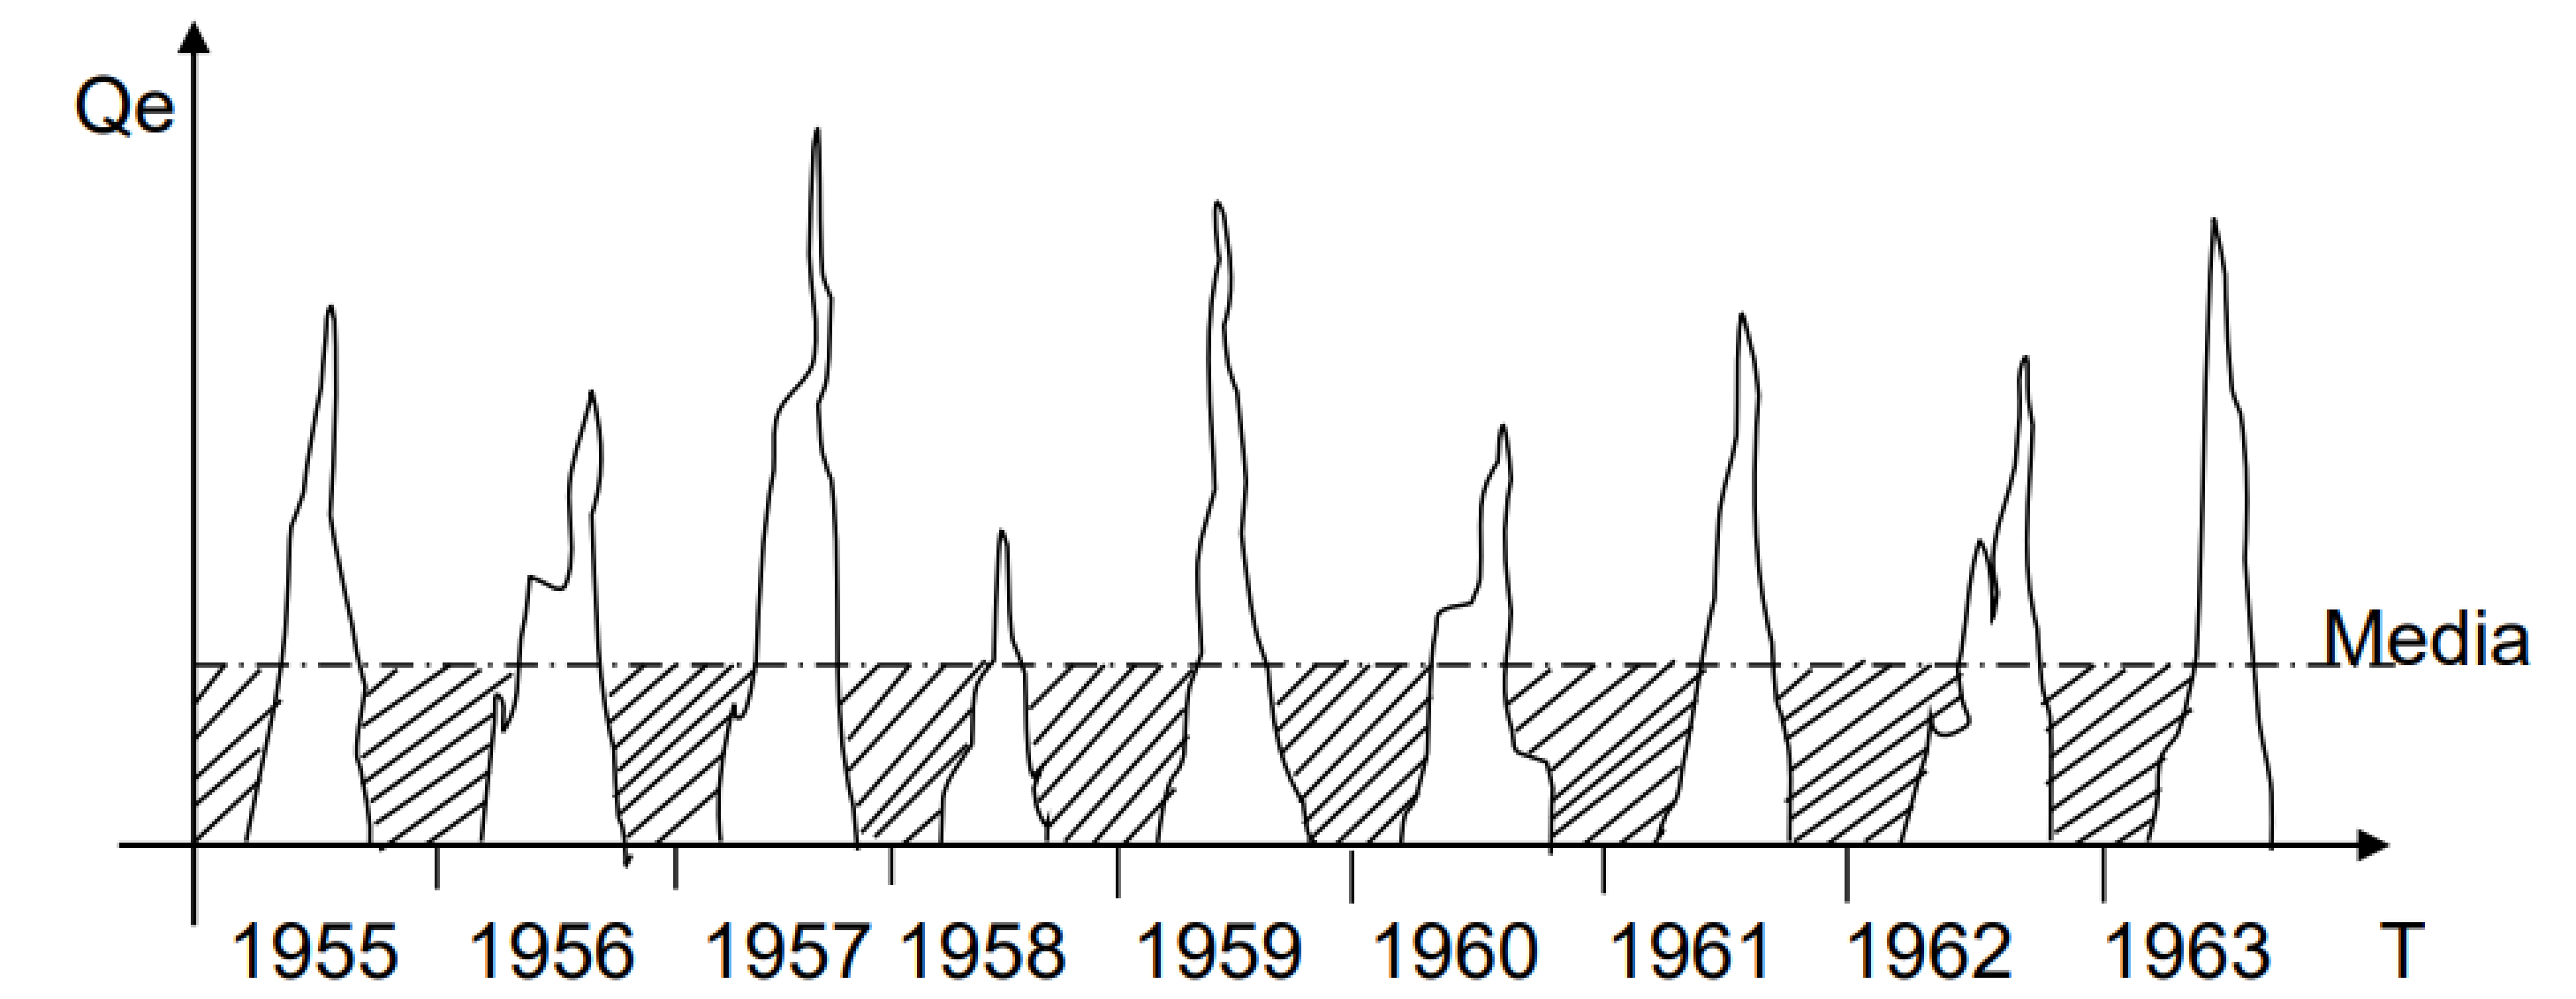
\includegraphics[width=0.5\textwidth]{fii20.png}}
	\caption{Hidrograma de una corriente intermitente.}
	\label{fii20}
\end{figure}
La necesidad de regularizar los escurrimientos de este tipo de corrientes, exige
la construcción de una \textbf{presa de almacenamiento}.
\begin{figure}[h!]
	\centerline{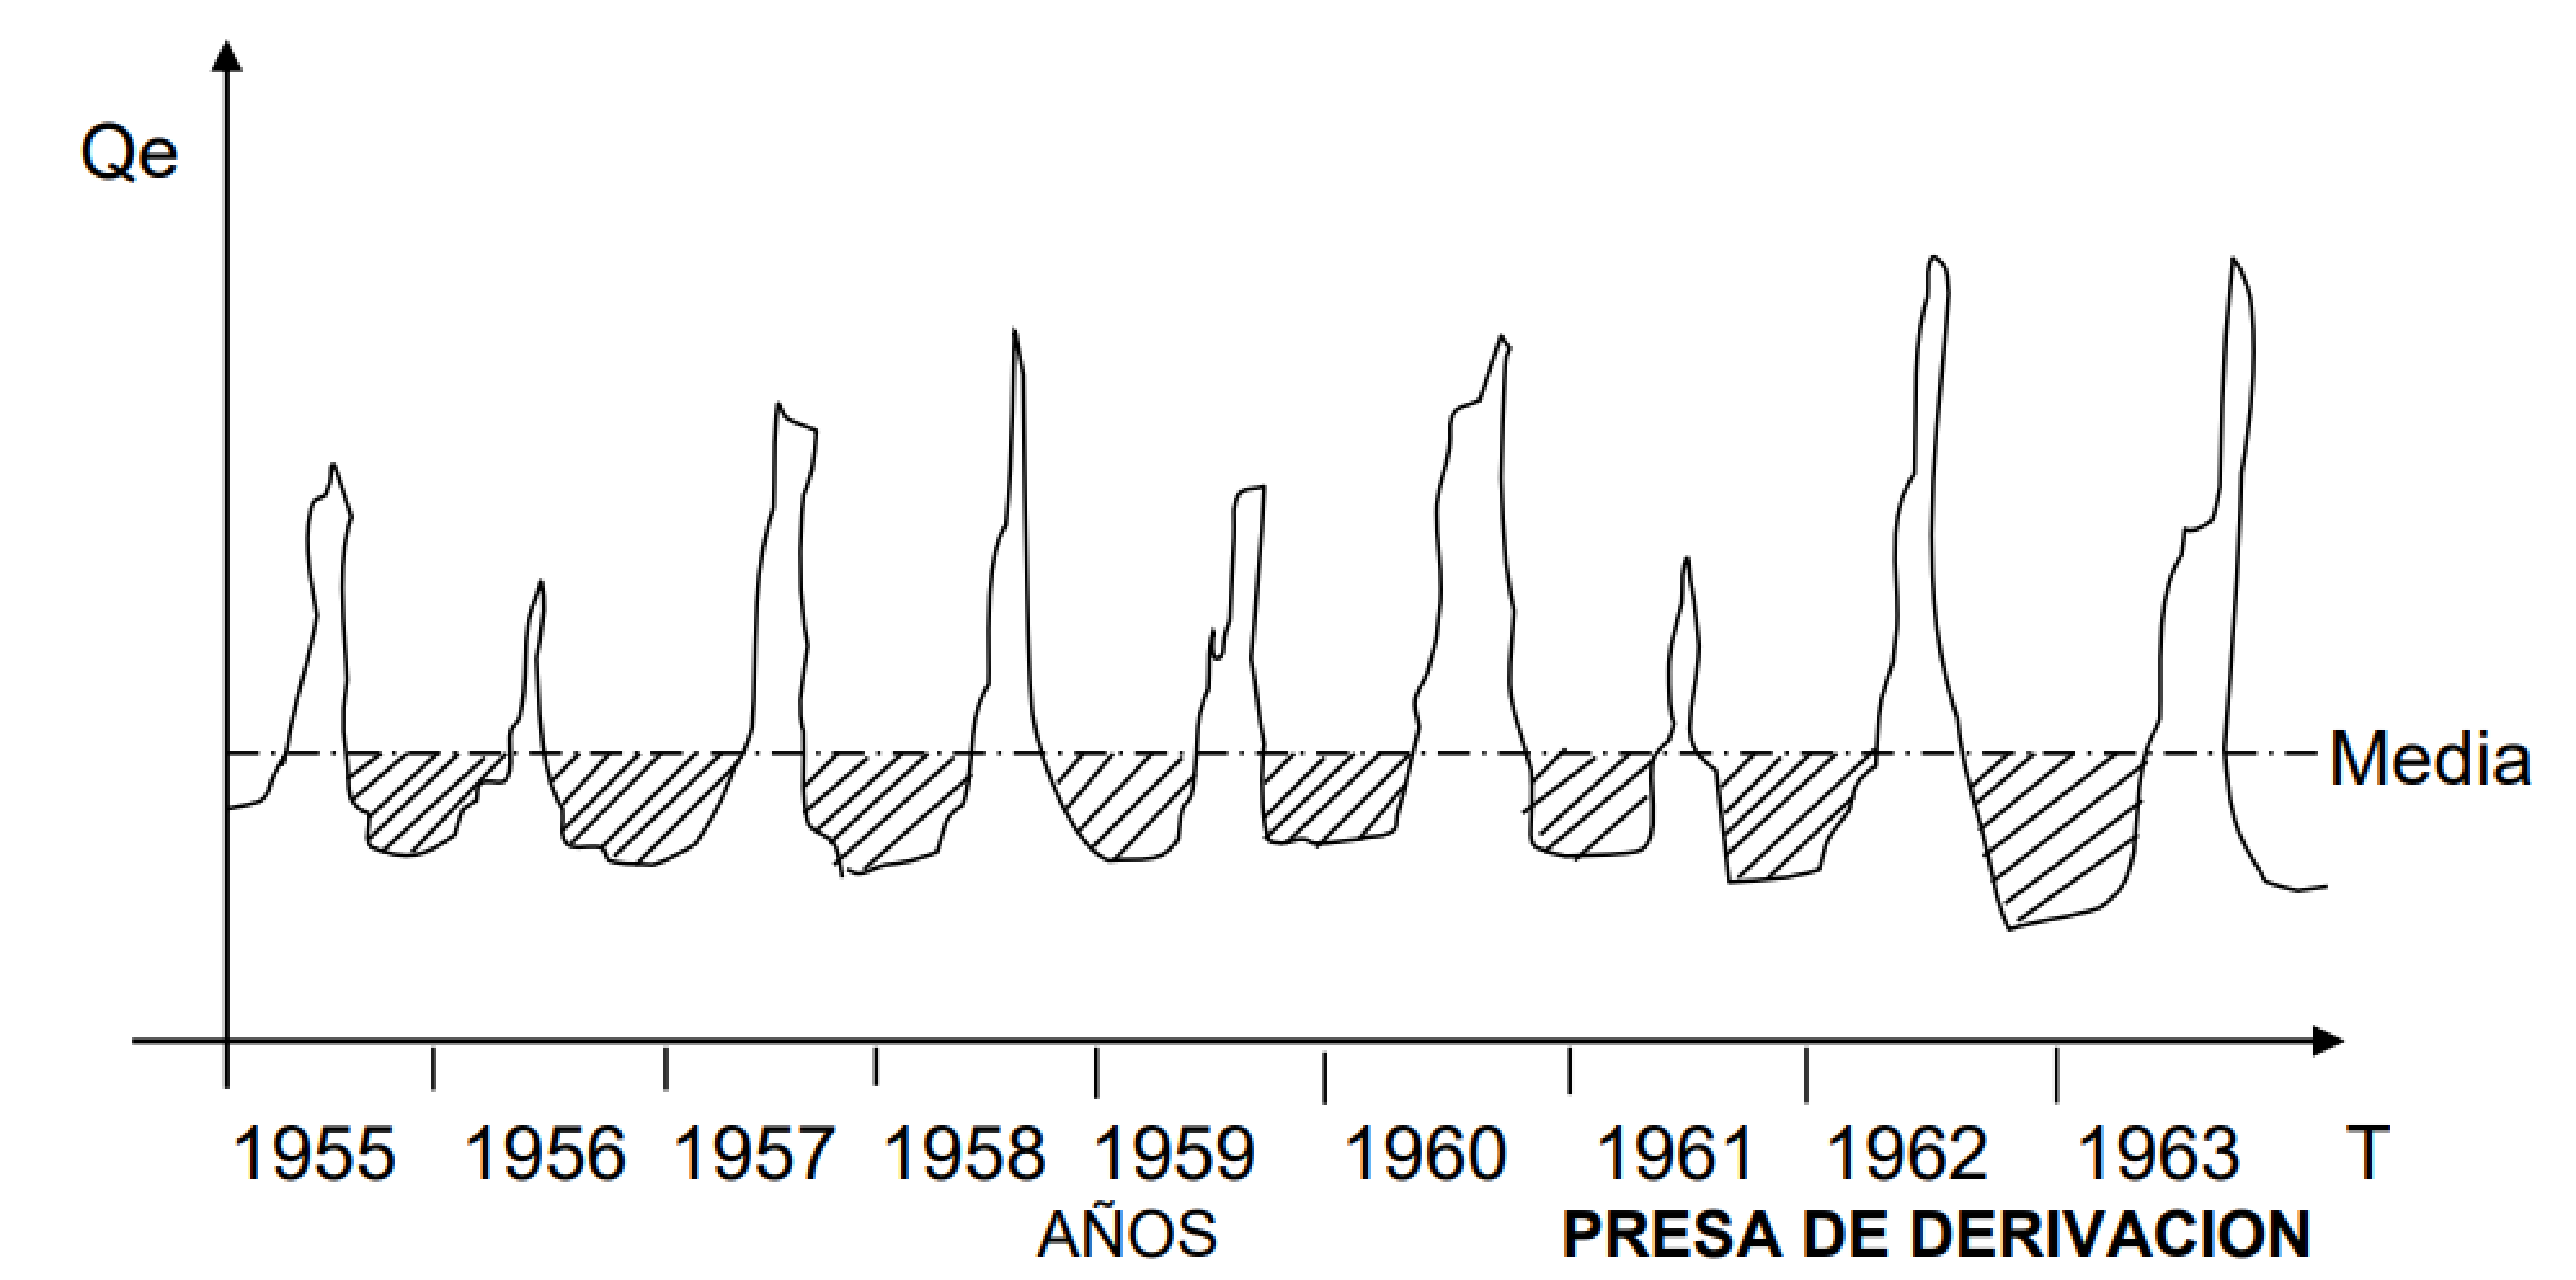
\includegraphics[width=0.5\textwidth]{fii21.png}}
	\caption{Hidrograma de una corriente permanente con caudales reducidos.}
	\label{fii21}
\end{figure}

\begin{figure}[h!]
	\centerline{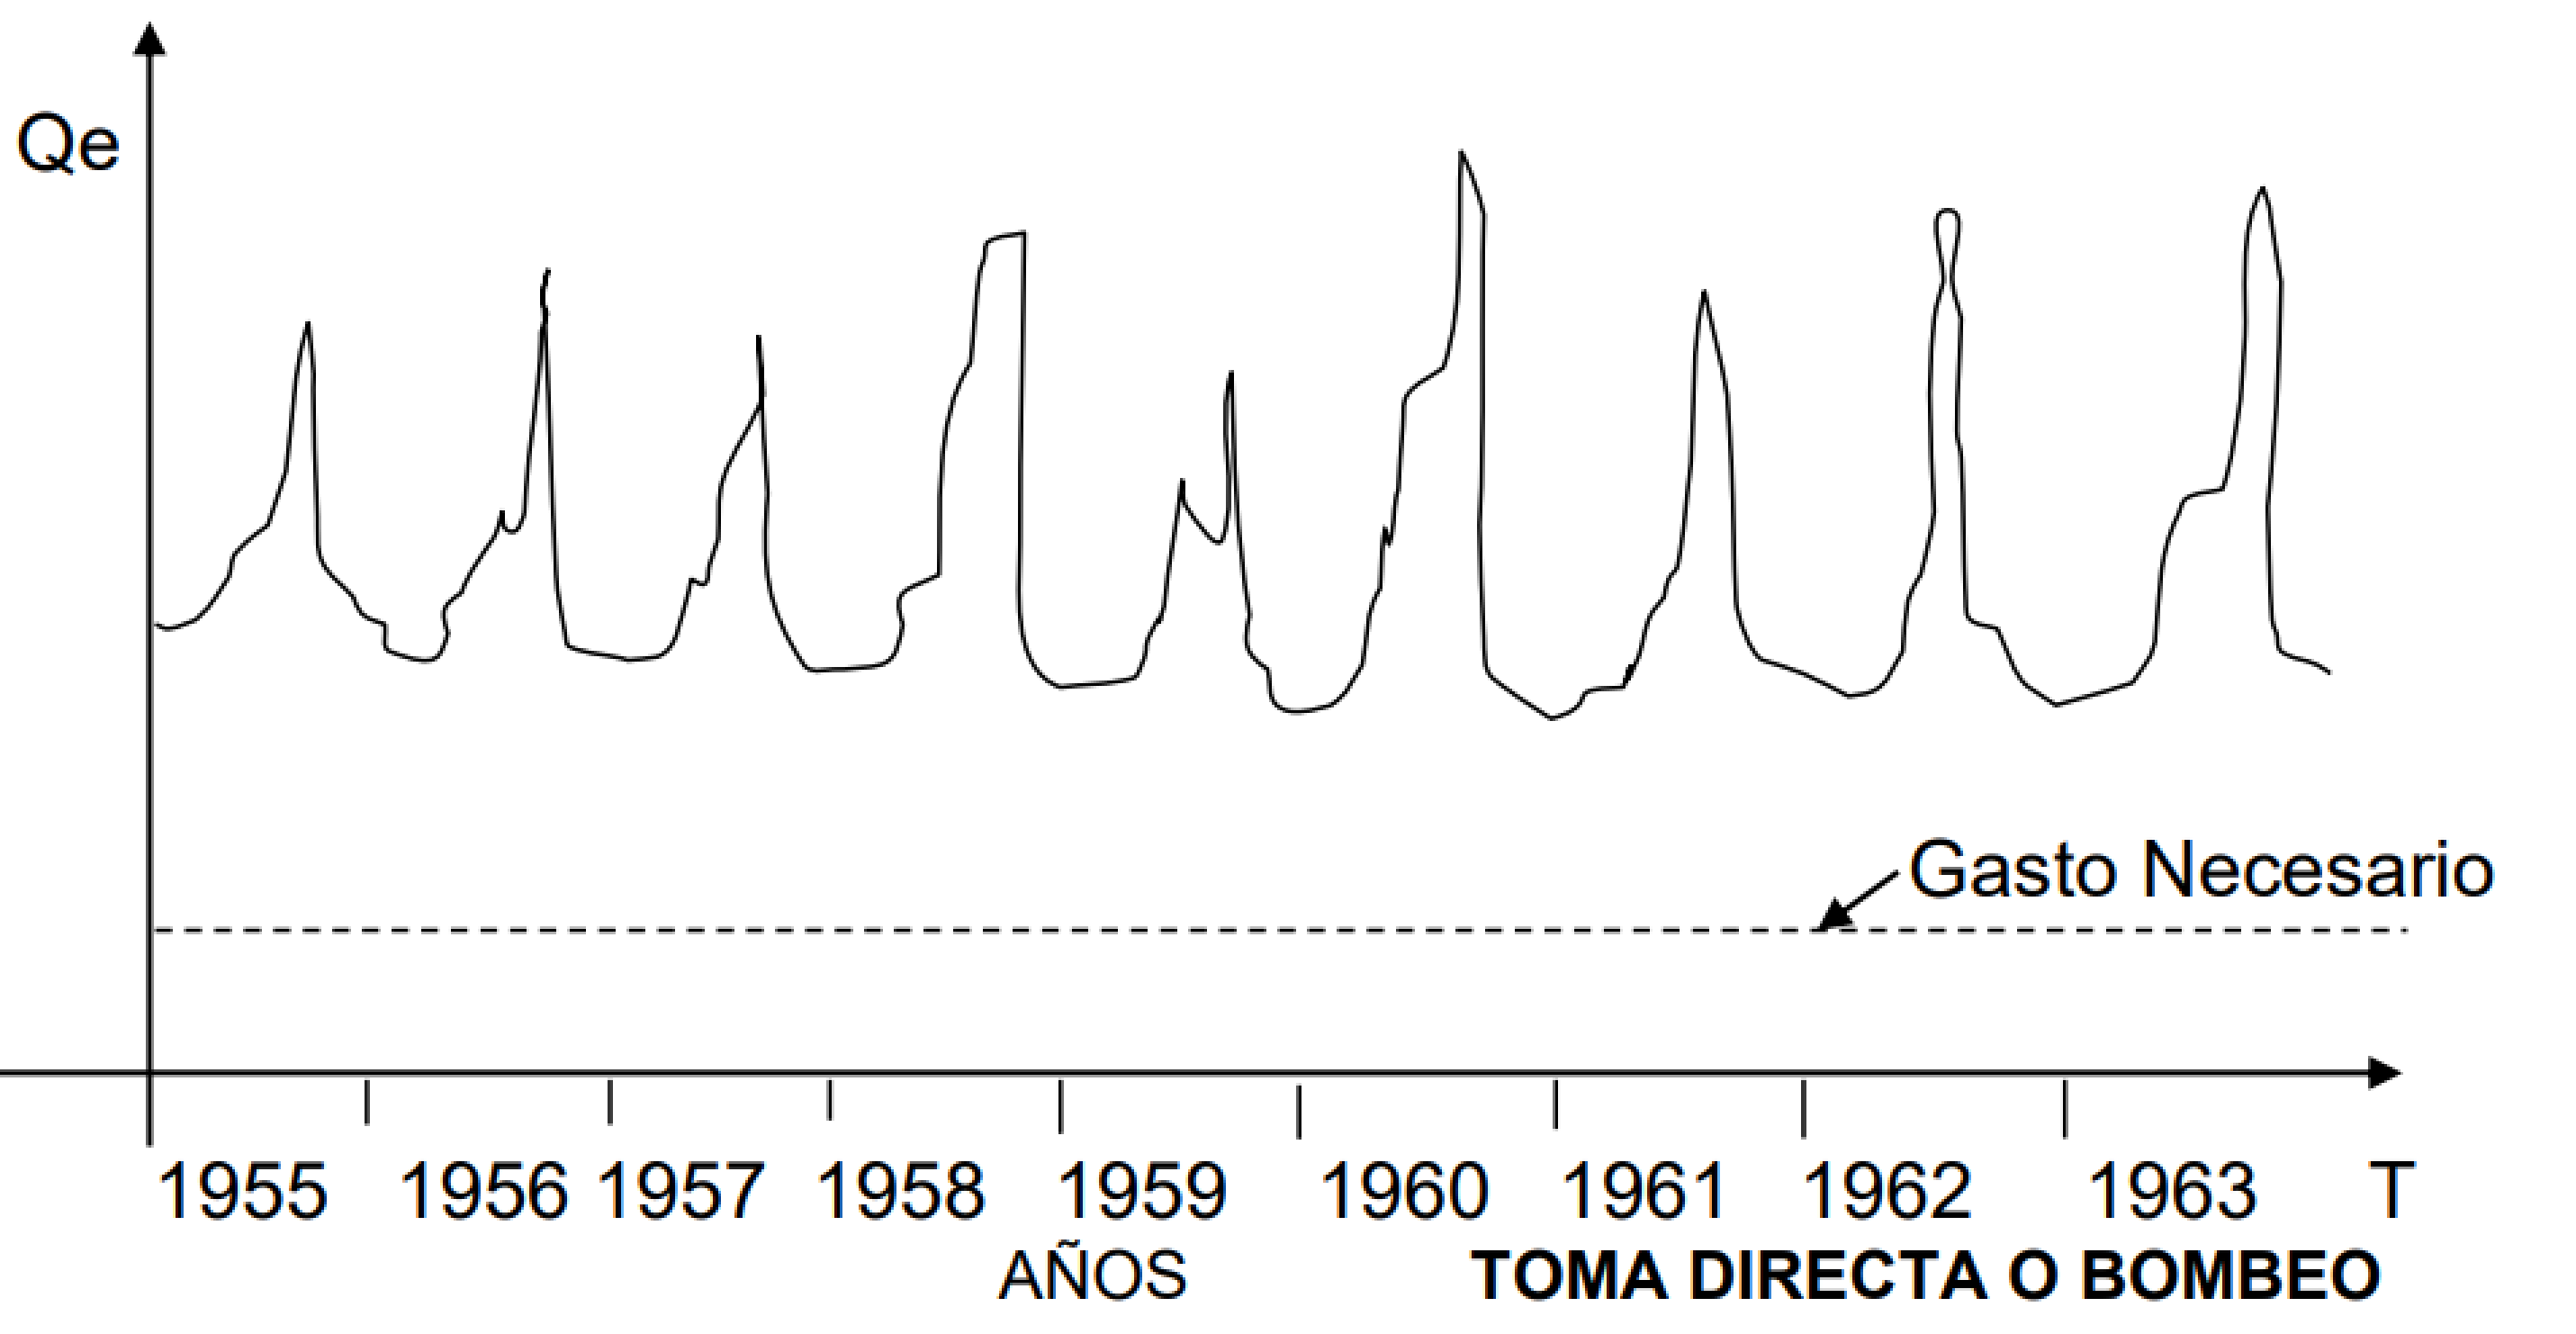
\includegraphics[width=0.5\textwidth]{fii22.png}}
	\caption{ Hidrograma de una corriente permanente con caudales acentuados.}
	\label{fii22}
\end{figure}

Las características de la corriente indica en principio el tipo de obra a construir. El estudio Hidrológico, comprende:

\begin{enumerate}
	\item Régimen del escurrimiento
	\item Régimen de demandas
	      \begin{enumerate}
		      \item Programa de cultivos
		      \item Plan de riegos
	      \end{enumerate}
\end{enumerate}


\begin{equation}
	L_{B}= \frac{V_{A.R.}}{S_{C.R.}}
\end{equation}

$L_{B} = (1{.}06m , 1{.}17m)$ (Promedio: $1{.}00m \approx 10,000 m^3$/Ha/año)

Donde $L_{B}$ es la lámina de riego bruta, en $m$, $V_{A.R.}$ Es el volumen de agua de riego, en $m^3$ y
$S_{C.R.}$ Superficie cosechada de riego, en $m^2 $

\subsubsection{Tipos de sistema de de Riego por Gravedad}

\begin{enumerate}
	\item \textbf{Con almacenamiento:} Este sistema de riego está conformado con una presa de almacenamiento como
	      fuente de abastecimiento principal, así como con una serie de canales y sus
	      estructuras que permiten llevar el agua de la presa hasta los lotes o parcelas de riego
	      donde se encuentran los cultivos.
	\item \textbf{Con almacenamiento y derivación}: Este sistema se presenta cuando la distancia entre la presa de almacenamiento
	      y la zona de riego es considerable, y entonces se utiliza un tramo de cauce como parte
	      del sistema de conducción, teniendo que proyectar una Presa derivadora aguas abajo
	      para poder extraer del mismo el agua y entregarla a un canal.
	\item \textbf{Mediante derivación:} Cuando por las condiciones del escurrimiento este se presenta en forma
	      permanente, presentándose en la época de estiaje un caudal de una magnitud
	      relativamente pequeña, entonces se puede plantear un sistema de riego por gravedad
	      mediante una derivación.
	\item \textbf{Con almacenamiento, derivación y bombeo:} Otras alternativas de explotación de las aguas superficiales, es cuando la zona
	      por beneficiar se encuentra en niveles superiores a donde se ubica la fuente de
	      abastecimiento, y entonces los aprovechamientos son por bombeo, si a esto se
	      adiciona que el origen del agua es de escurrimiento superficial en corriente intermitente
	      y la zona de riego se presenta a una cierta distancia de la fuente de abastecimiento,
	      entonces se presenta el Sistema de riego por gravedad con almacenamiento,
	      derivación y bombeo.
	\item \textbf{Mediante bombeo:} Cuando se tiene una fuente de abastecimiento cuyo origen del agua es
	      superficial, como un lago, laguna, o río, o su origen es subterráneo como manantiales
	      o galerías filtrantes, y el aprovechamiento se encuentra a niveles superiores a donde se
	      ubica la fuente entonces el sistema de riego por gravedad planteado es exclusivamente
	      por bombeo teniendo que conformarse una obra que se denomina Planta de Bombeo.
\end{enumerate}

\subsubsection{Partes constitutivas de un sistema de riego por gravedad}

El sistema de riego por gravedad a su vez se constituye por una serie de
subsistemas:

\begin{enumerate}
	\item Subsistema de almacenamiento
	\item Subsistema de conducción
	\item Subsistema de derivación
	\item Subsistema de distribución
	\item Subsistema de drenaje
	\item Subsistema de comunicaciones y obras diversas.
\end{enumerate}
\begin{figure}[h!]
	\centerline{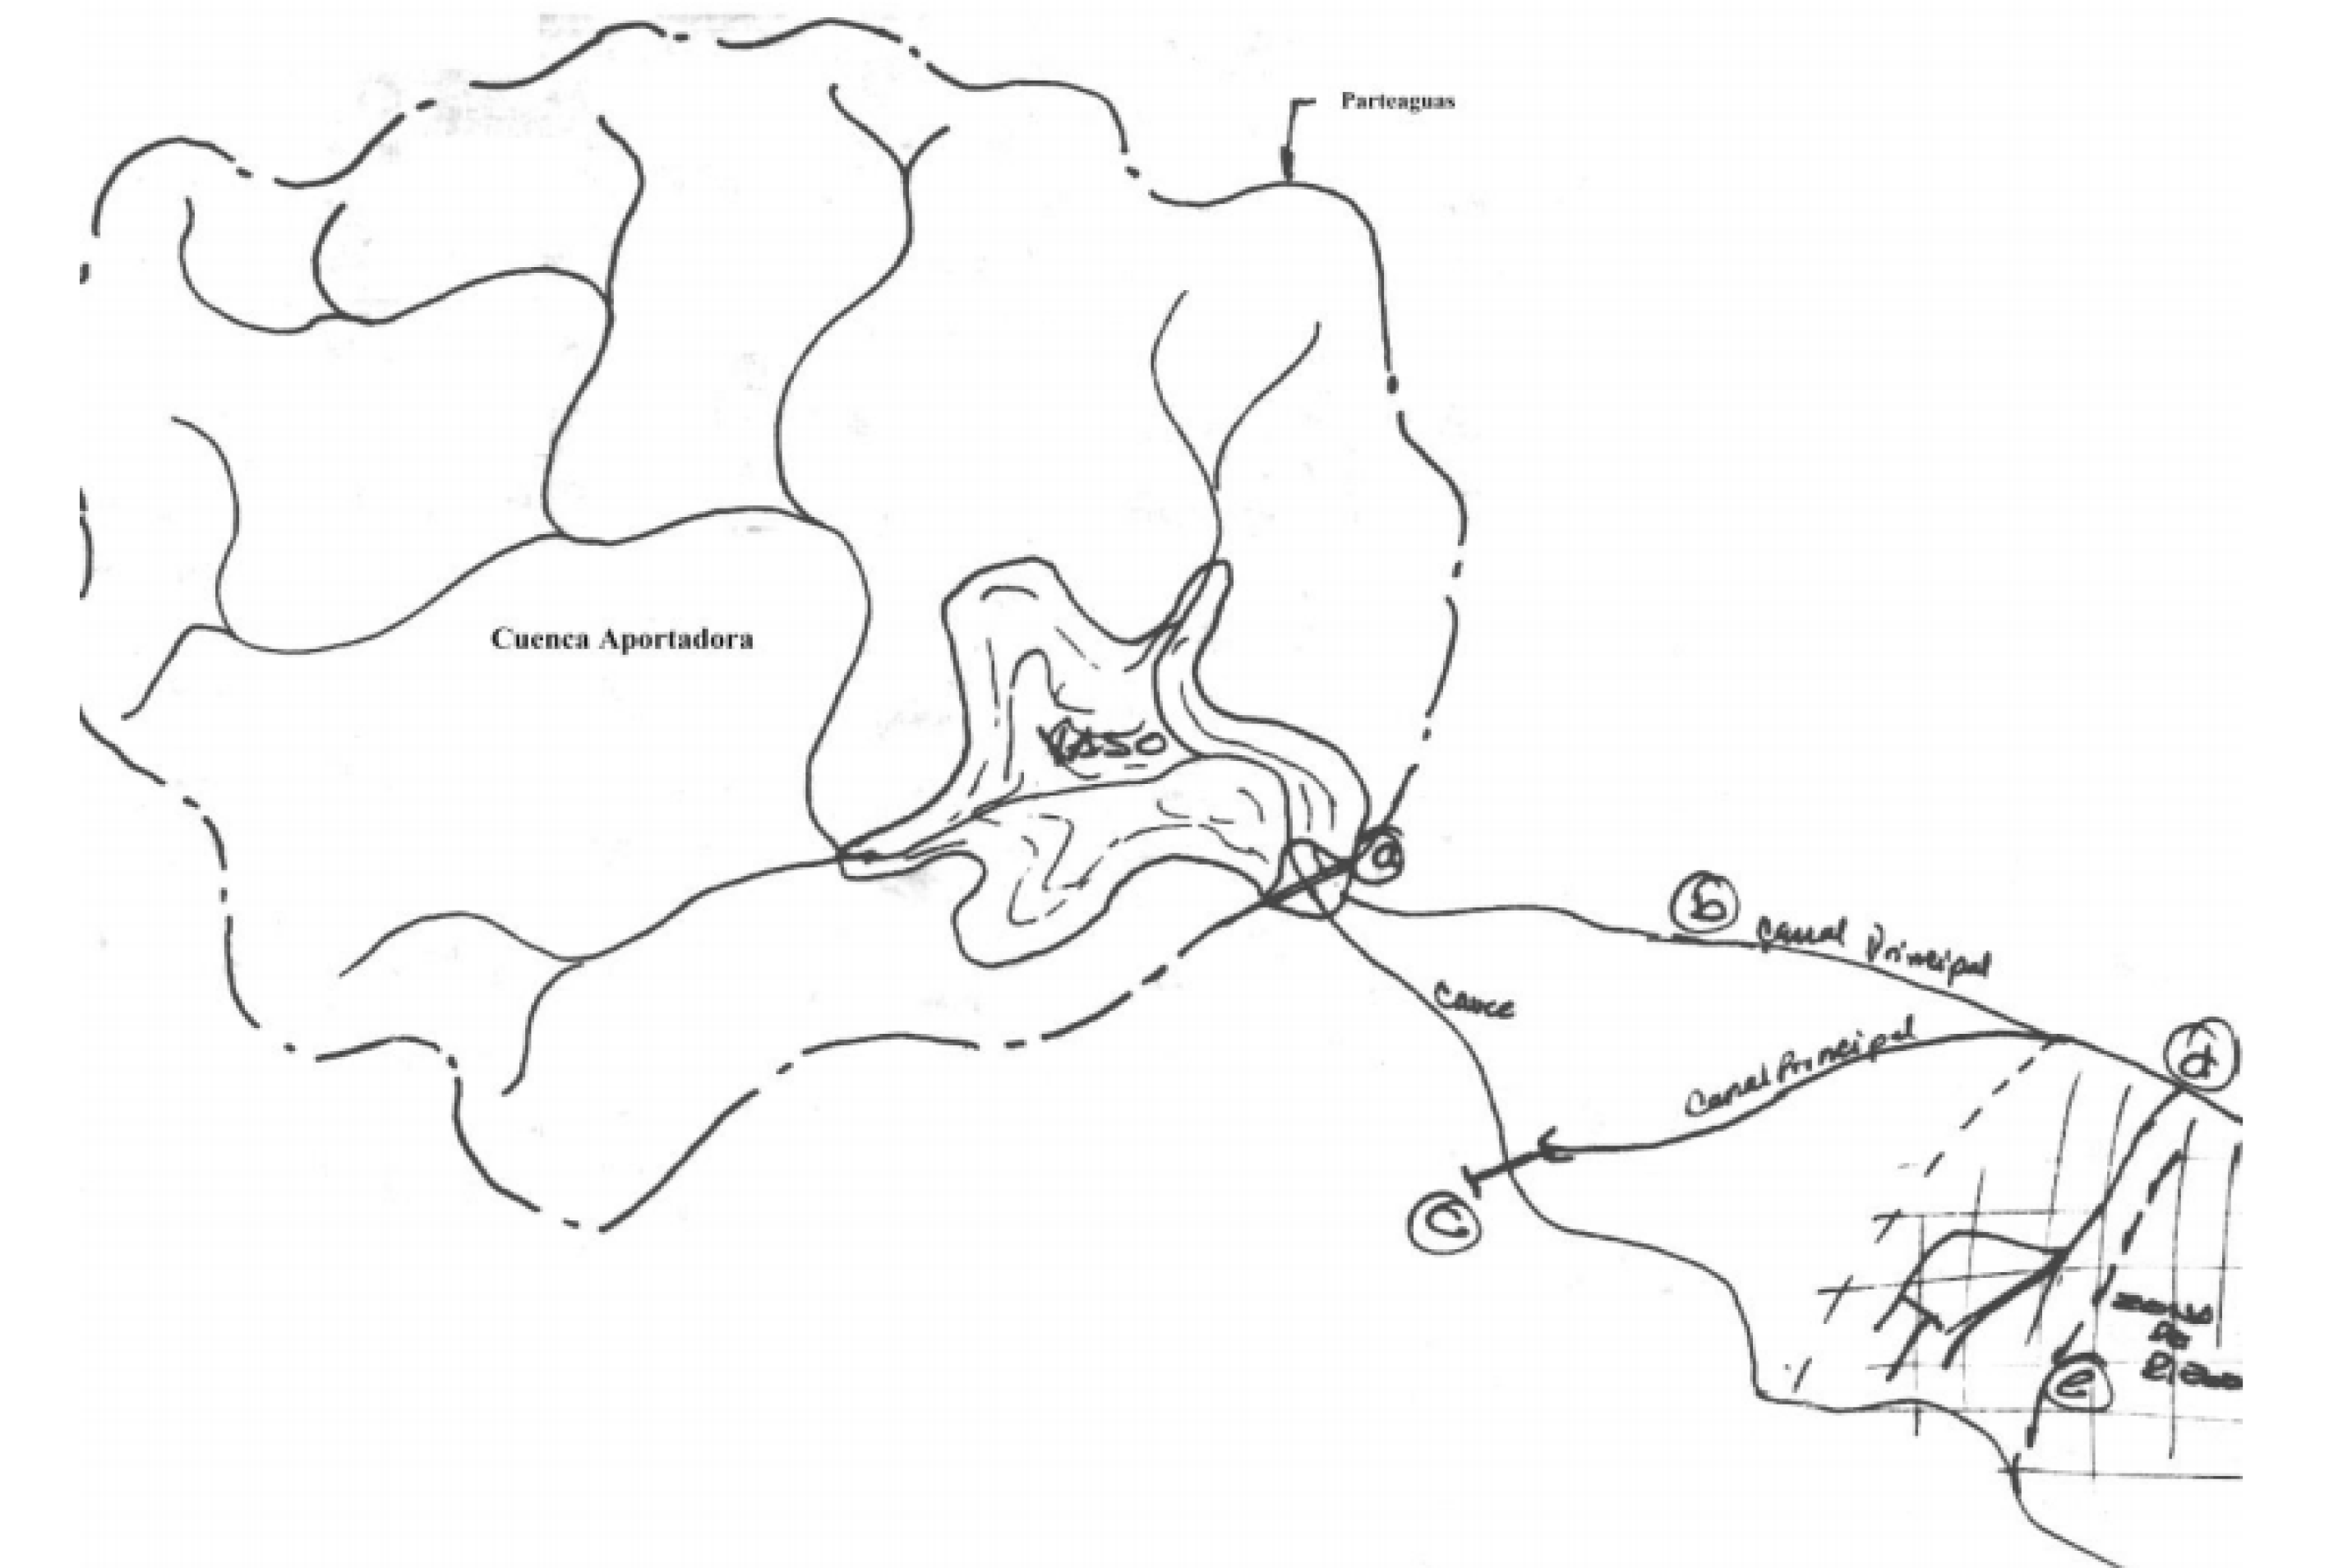
\includegraphics[width=0.7\textwidth]{fii23.png}}
	\caption{Esquema genérico de un sistema de riego por gravedad completo.}
	\label{fii23}
\end{figure}

\subsubsection{Partes constitutivas de un sistema de riego por bombeo.}

En general las partes constitutivas de un sistema de riego por bombeo son las
mismas que las de un sistema de riego por gravedad, con la única diferencia es que se
ubica a continuación de la fuente de abastecimiento una planta de bombeo que va a
permitir ubicar el agua a un nivel suficiente para dominar toda la superficie de riego
mediante gravedad, buscando que esta ubicación sea en la forma más económica a
través de ubicar una mínima diferencia de niveles y en el menor recorrido posible.

\begin{figure}[h!]
	\centerline{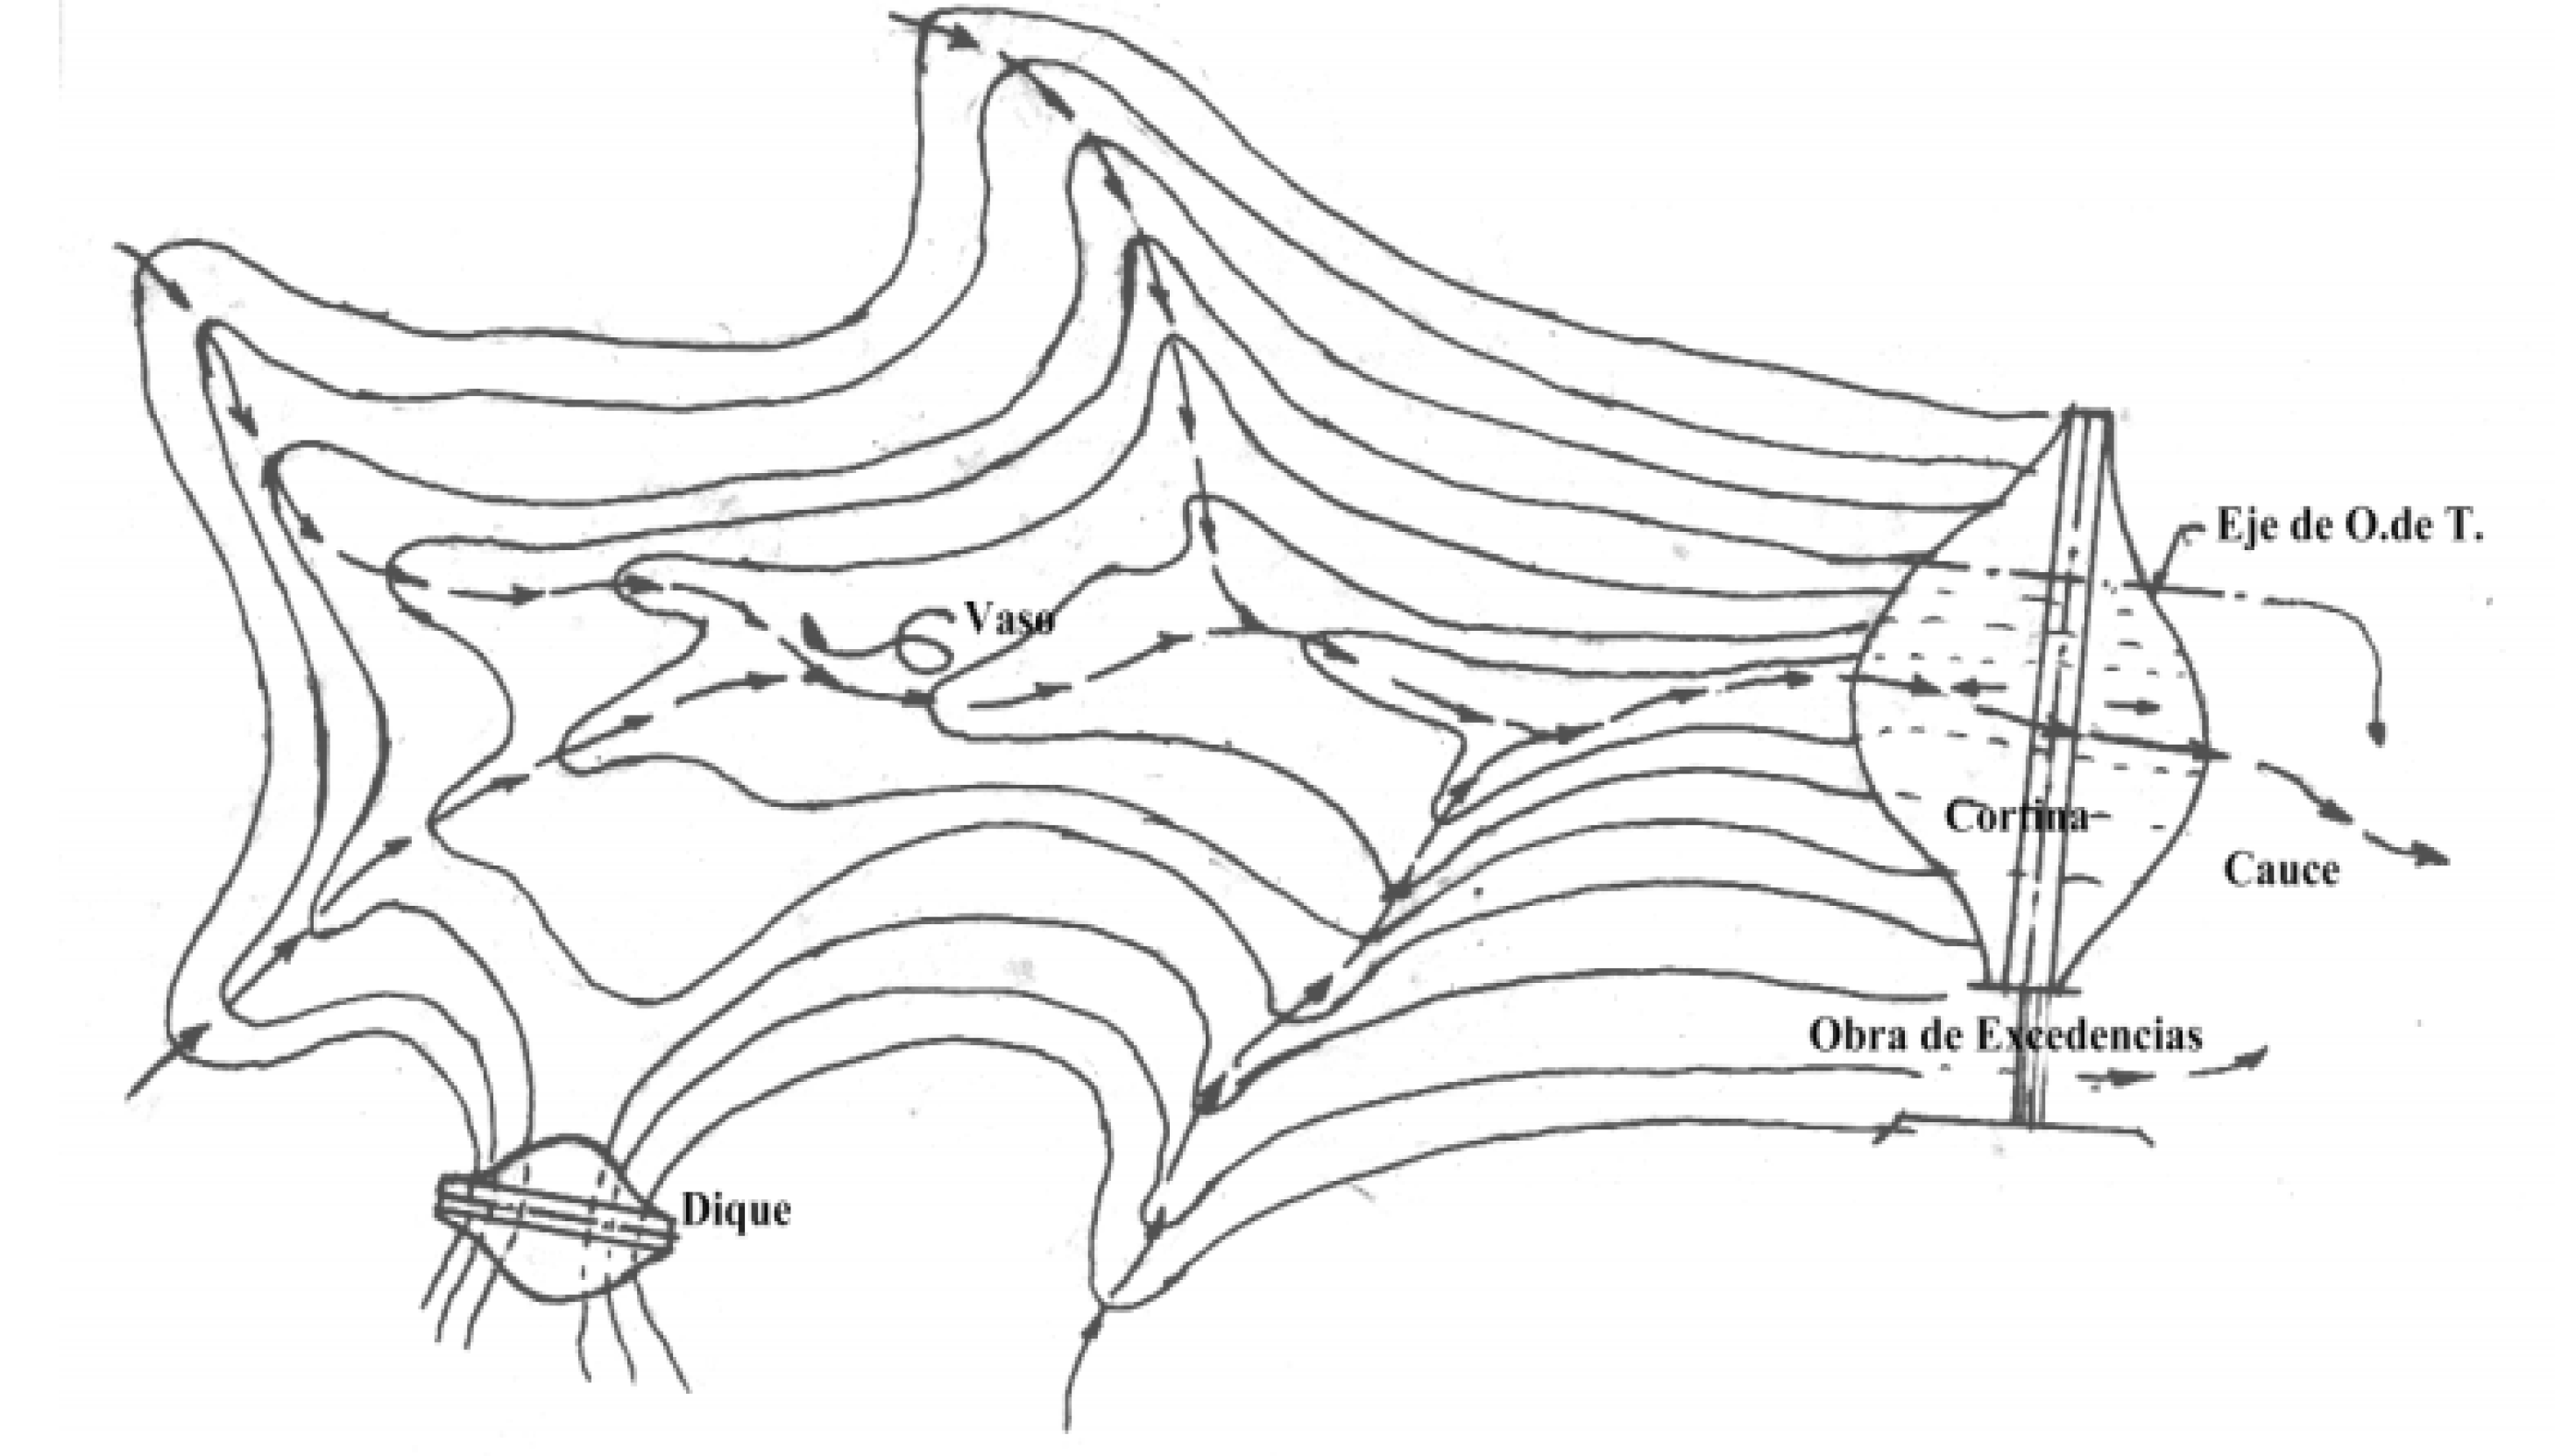
\includegraphics[width=0.5\textwidth]{fii24.png}}
	\caption{Planta Esquemática de Presa y Vaso de almacenamiento}
	\label{fii24}
\end{figure}

\section{Sistema de almacenamiento}
\subsection{Partes constitutivas y funciones}
\begin{definition}[Obra de retención (o cortina)]
	La función de esta es retener las aguas para
	formar el vaso de almacenamiento y regular los escurrimientos del cauce.
\end{definition}

\begin{definition}[Obra de toma]
	La función de esta obra es manejar las extracciones para
	satisfacer la demanda que los diferentes beneficios exigen.
\end{definition}

\begin{definition}[Obra de excedencias]
	La función es dar salida a las aguas de escurrimiento que
	no pueden ser almacenadas por haber llegado a un cierto nivel que muestra la
	capacidad total.
\end{definition}

Estas tres estructuras, por lo general forman las \textbf{presa de Almacenamiento}.

\begin{definition}[Diques de cierre]
	La función es ayudar a la cortina al cierre del vaso, en puertos
	naturales independientes de la boquilla.
\end{definition}

\subsection{Elementos naturales y sus condiciones de los sistemas de almacenamiento}

\begin{definition}[Cuenca]
	Es la superficie de terreno limitada por la línea del parteaguas, en la cual el agua
	de lluvia precipitada dentro del área, escurre para ser drenada por el río o arroyo,
	desde su nacimiento hasta el sitio de la boquilla.
	Las características de tamaño, forma, vegetación, pendientes, corrientes, etc$\dots$
	son condiciones que influyen en el escurrimiento y adecuada alimentación al vaso.
\end{definition}

\begin{definition}[Vaso de almacenamiento]
	Valle en cual se puede crear un receptáculo topográfico para almacenar agua,
	mediante el cierre de una boquilla con una estructura para formar un lago artificial.
	Las características de capacidad e impermeabilidad, son condiciones favorables
	para un adecuado almacenamiento. Topografía: implica Gráfica de Áreas-Capacidades;
	Geología: implica Impermeabilidad; Problemas: Calizas cavernosas (yeso y grietas).
\end{definition}

\begin{definition}[Boquilla]
	Estrechamiento topográfico de un valle donde se construye la estructura de
	retención o cortina. Condiciones favorables: Resistencia, impermeabilidad, topografía implica
	Topografía Forma y tamaño; Geología implica Resistencia e impermeabilidad
\end{definition}

\begin{definition}[Cauce]
	Conducto natural por el cual escurre el agua. Su estudio es importante por el
	acarreo de sedimentos, así como por la permeabilidad.
\end{definition}

\subsection{Gráfica Áreas Capacidades}

Un vaso de almacenamiento topográficamente es un valle natural que tiene
como base un cauce por el cual escurre el agua que se ha precipitado en el área de la
cuenca y la cual es cerrada en el sitio denominado boquilla y sobre la que se proyecta y
construye una cortina o presa, cerrando así el sitio y conformando un gran lago
artificial.

Para conocer e identificar la forma de un vaso de almacenamiento es necesario
efectuar previamente un levantamiento topográfico que permita determinar su
capacidad a diferentes alturas de la cortina, para conocer las áreas de embalse a
diferentes elevaciones, con el objeto de poder estimar las pérdidas por evaporación, así
mismo el poder contar con un apoyo para la realización de los diferentes estudios
necesarios para poder cumplir con las exigencias que plantea el proyecto de una presa
de almacenamiento, entre otros los estudios geológicos que permitan conocer el grado
de impermeabilidad del vaso, así como el poder identificar la superficie de las
propiedades inundadas que sirvan de base para las indemnizaciones correspondientes
ante las afectaciones que necesariamente tendrán que presentarse.

\begin{figure}[h!]
	\centerline{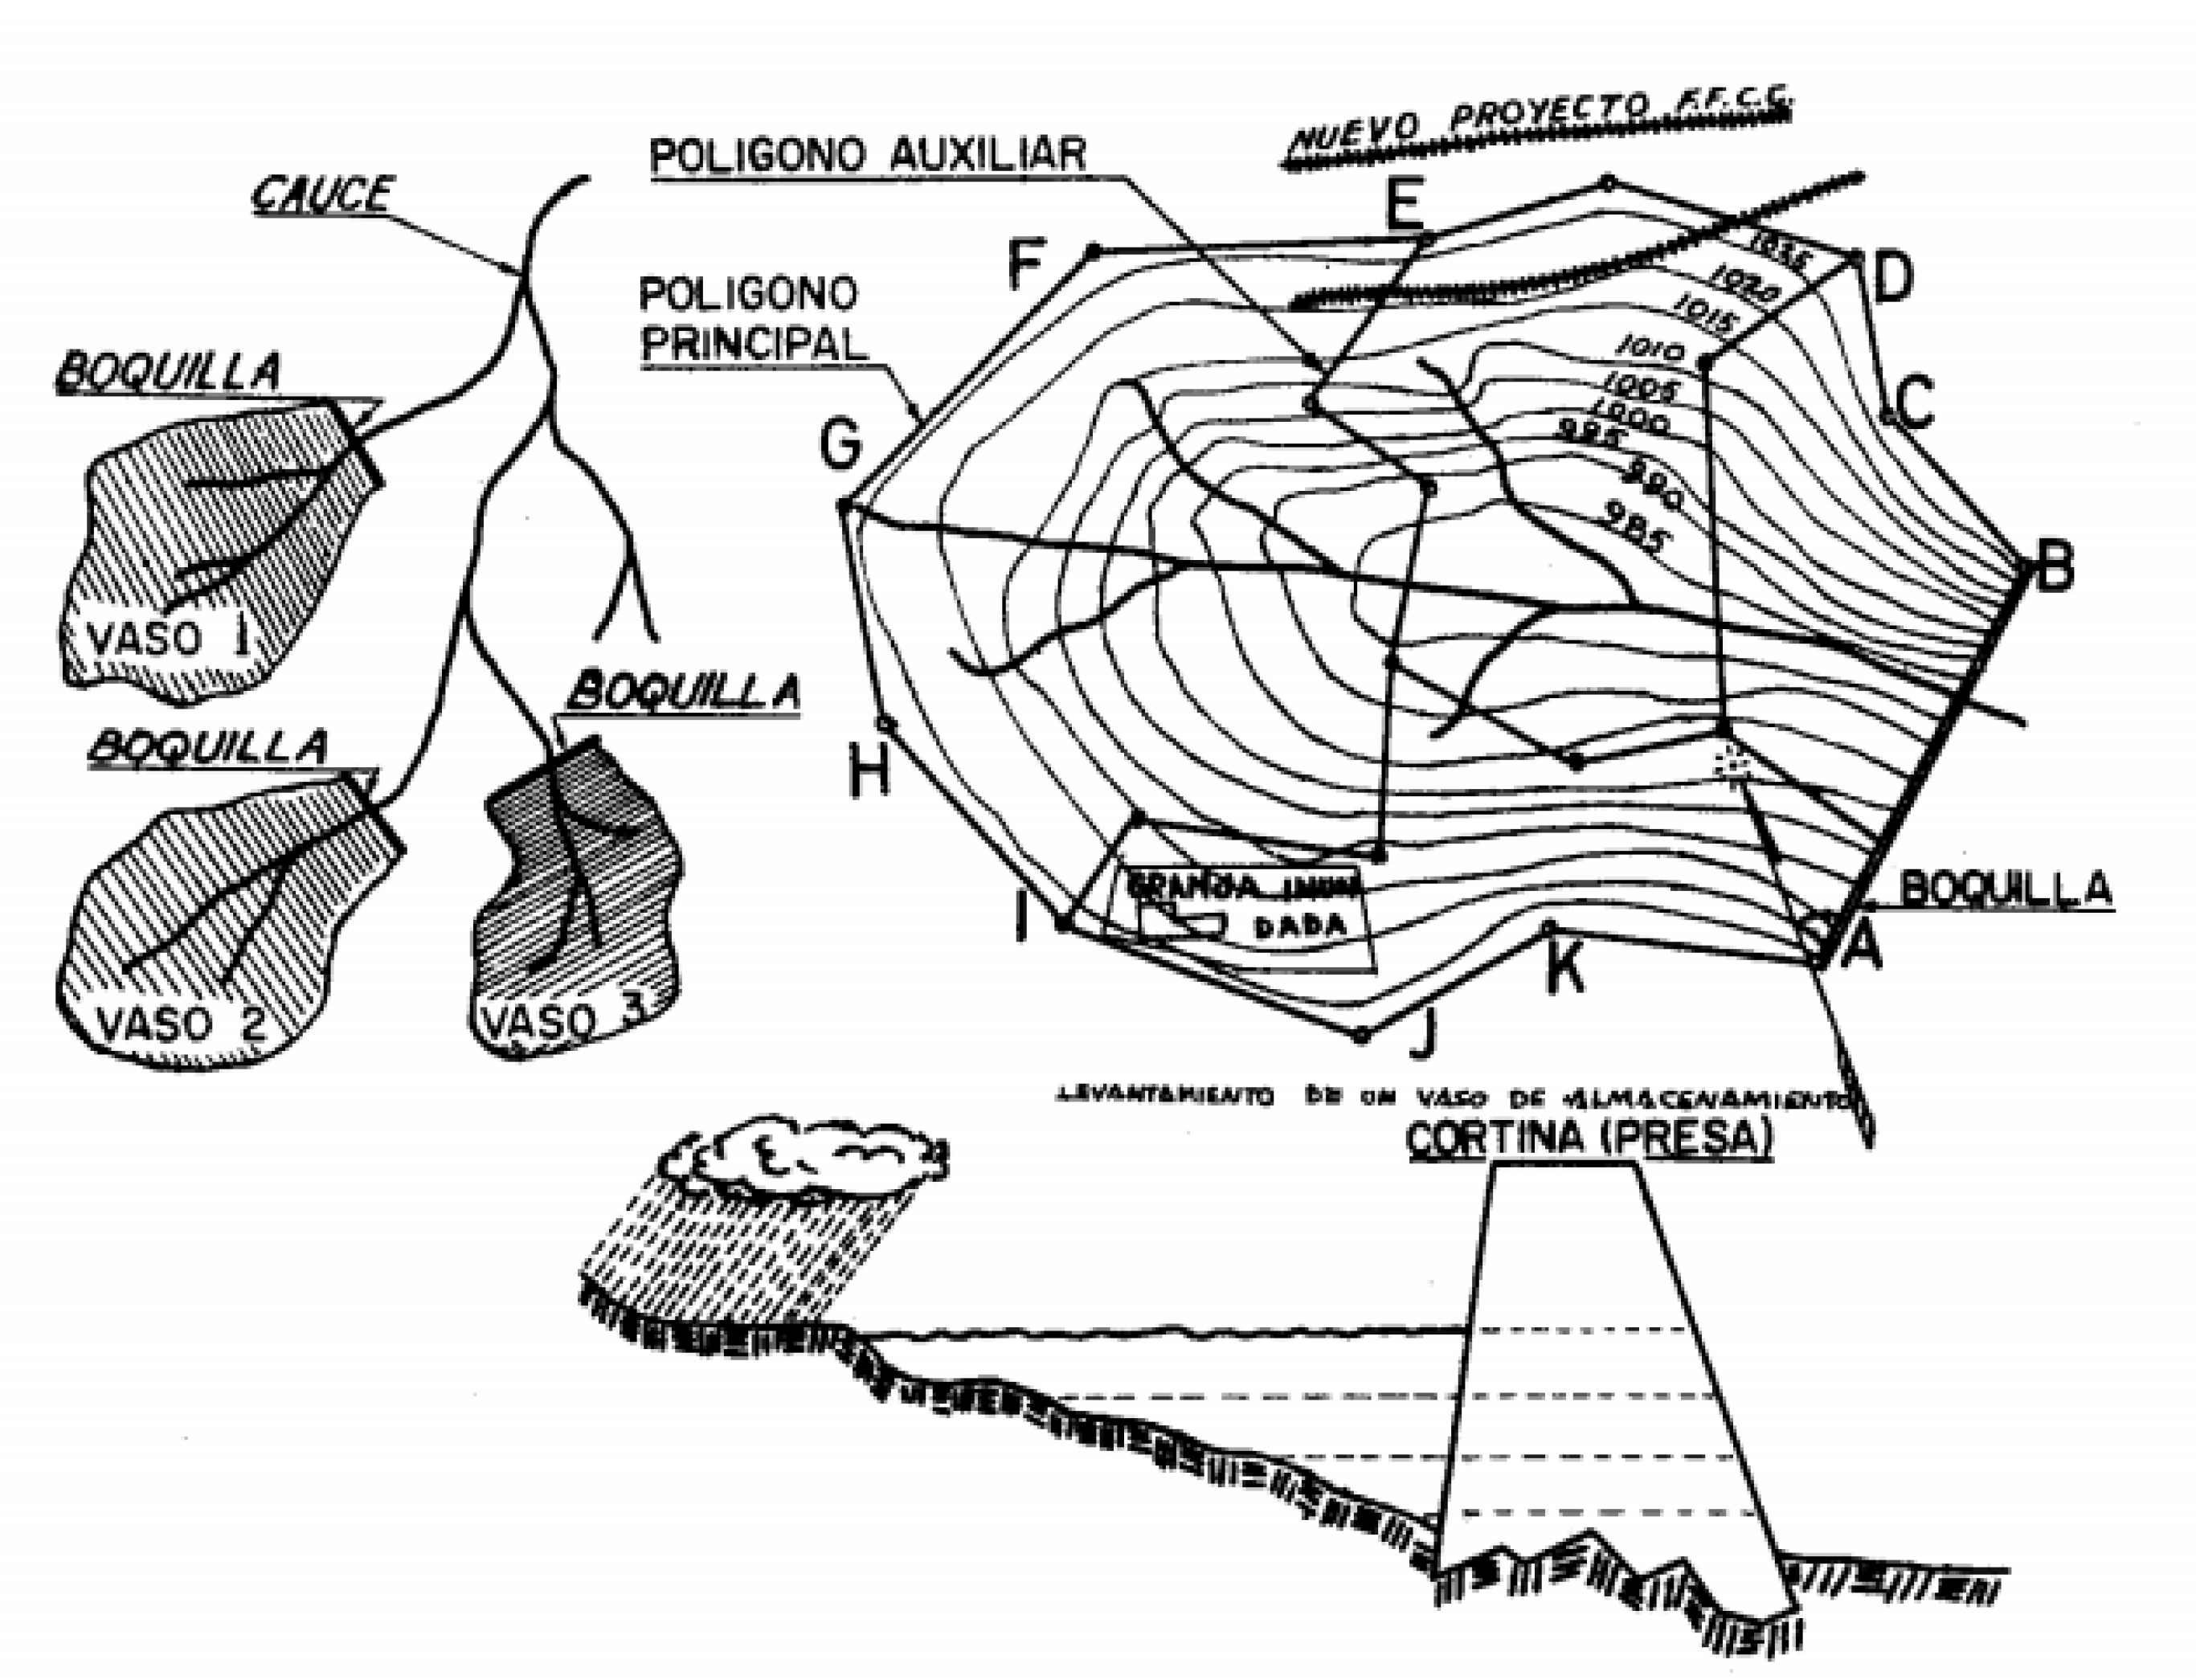
\includegraphics[width=0.5\textwidth]{fii25.png}}
	\caption{Levantamiento topográfico de un vaso de almacenamiento}
	\label{fii25}
\end{figure}

Para poder construir las gráficas de Áreas y Capacidades, se
delimitará el vaso de almacenamiento trazando la línea que corresponde al eje
probable de la cortina, que cerrará desde el fondo del cauce, hasta la curva
correspondiente al nivel probable de las aguas máximas.
El área de cada una de las curvas de nivel, limitada hasta el eje probable de la
cortina se obtiene por medio de un integrador mecánico (planímetro). Se hace la
determinación de las áreas, desde la correspondiente al fondo del cauce, hasta la
correspondiente al nivel probable de las aguas máximas.
El volumen entre dos curvas de nivel consecutivas se obtiene multiplicando la
semisuma de las dos áreas, por la diferencia de elevaciones entre las dos curvas. Así
si la equidistancia es de $1m$, y el volumen comprendido entre las curvas cuyas
elevaciones son la $152m$ y la $153m$, el volumen está dado por:
\begin{equation}
	V_{152-153}= \left(\frac{S_{152}+S_{153}}{2} \right) \times 1{.}0
\end{equation}
La suma de elevaciones parciales, da la capacidad del vaso hasta la elevación
requerida. Con estos datos se forma una tabla y posteriormente se construye la
Gráfica.
\begin{figure}[h!]
	\centerline{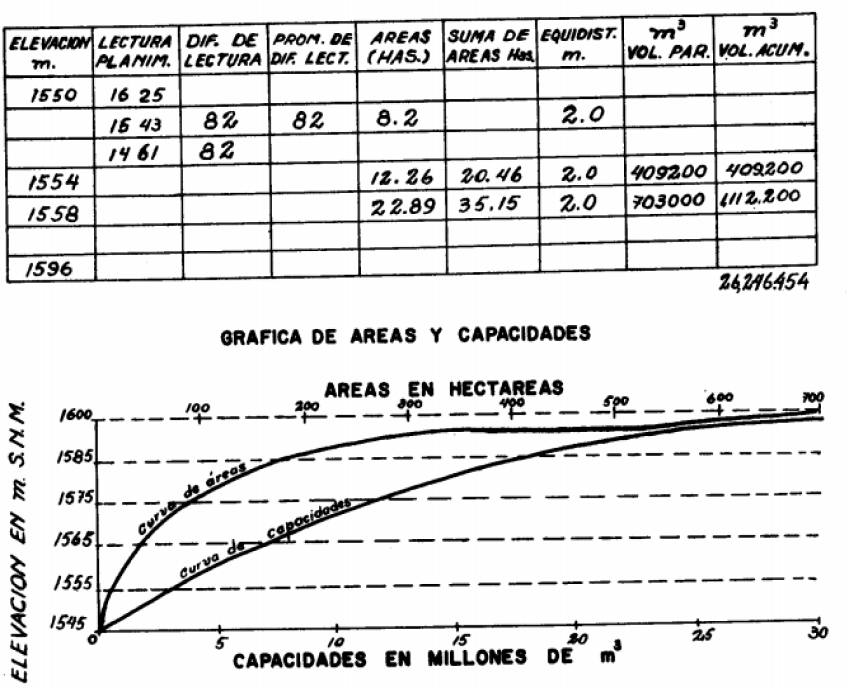
\includegraphics[width=0.5\textwidth]{fii26.png}}
	\caption{Gráfica de Áreas y capacidades en un vaso de almacenamiento.}
	\label{fii26}
\end{figure}
La graficación anterior es conveniente efectuarse en papel milimétrico bajo una
escala adecuada que permita hacer una lectura precisa y confiable en las elevaciones,
áreas y capacidades.

\subsection{Capacidades de almacenamiento y altura de la presa}
\begin{enumerate}
	\item \textbf{Capacidades de almacenamiento y Elevaciones físicas:} Las capacidades fundamentales que identifican a un almacenamiento son:
	      \begin{enumerate}
		      \item \textbf{Capacidad muerta $(C_{M})$:} es el volumen del almacenamiento el cual por su
		            condición nunca puede ser extraído del vaso por gravedad, para satisfacer beneficios
		            que se encuentren aguas abajo del mismo, y queda conformado con el volumen de
		            azolves y otros (Volumen para cría de peces, volumen para recreación y turismo,
		            volumen para abrevadero de ganado, etc$\dots$). Esta capacidad queda definida por el Nivel
		            de Almacenamiento mínimo \textbf{(N.A.min.)} la cual a su vez identifica a la cota física de la
		            obra de toma.
		      \item \textbf{Capacidad Total del almacenamiento \textbf{(CTA)}} es el volumen máximo que
		            puede ser retenido dentro del vaso, para cuando se tienen vertedores de cresta libre.
		            Esta capacidad queda definida por el Nivel de Aguas Normales (N.A.N.), algunos
		            autores le denominan N.A.M.O. (Nivel de Aguas Máximas de Operación), esta cota
		            identifica la cota física correspondiente al nivel de la cresta del vertedor de excedencias
		            (Obra de excedencias) cuando este tiene descarga libre.
		            \begin{figure}[h!]
			            \centerline{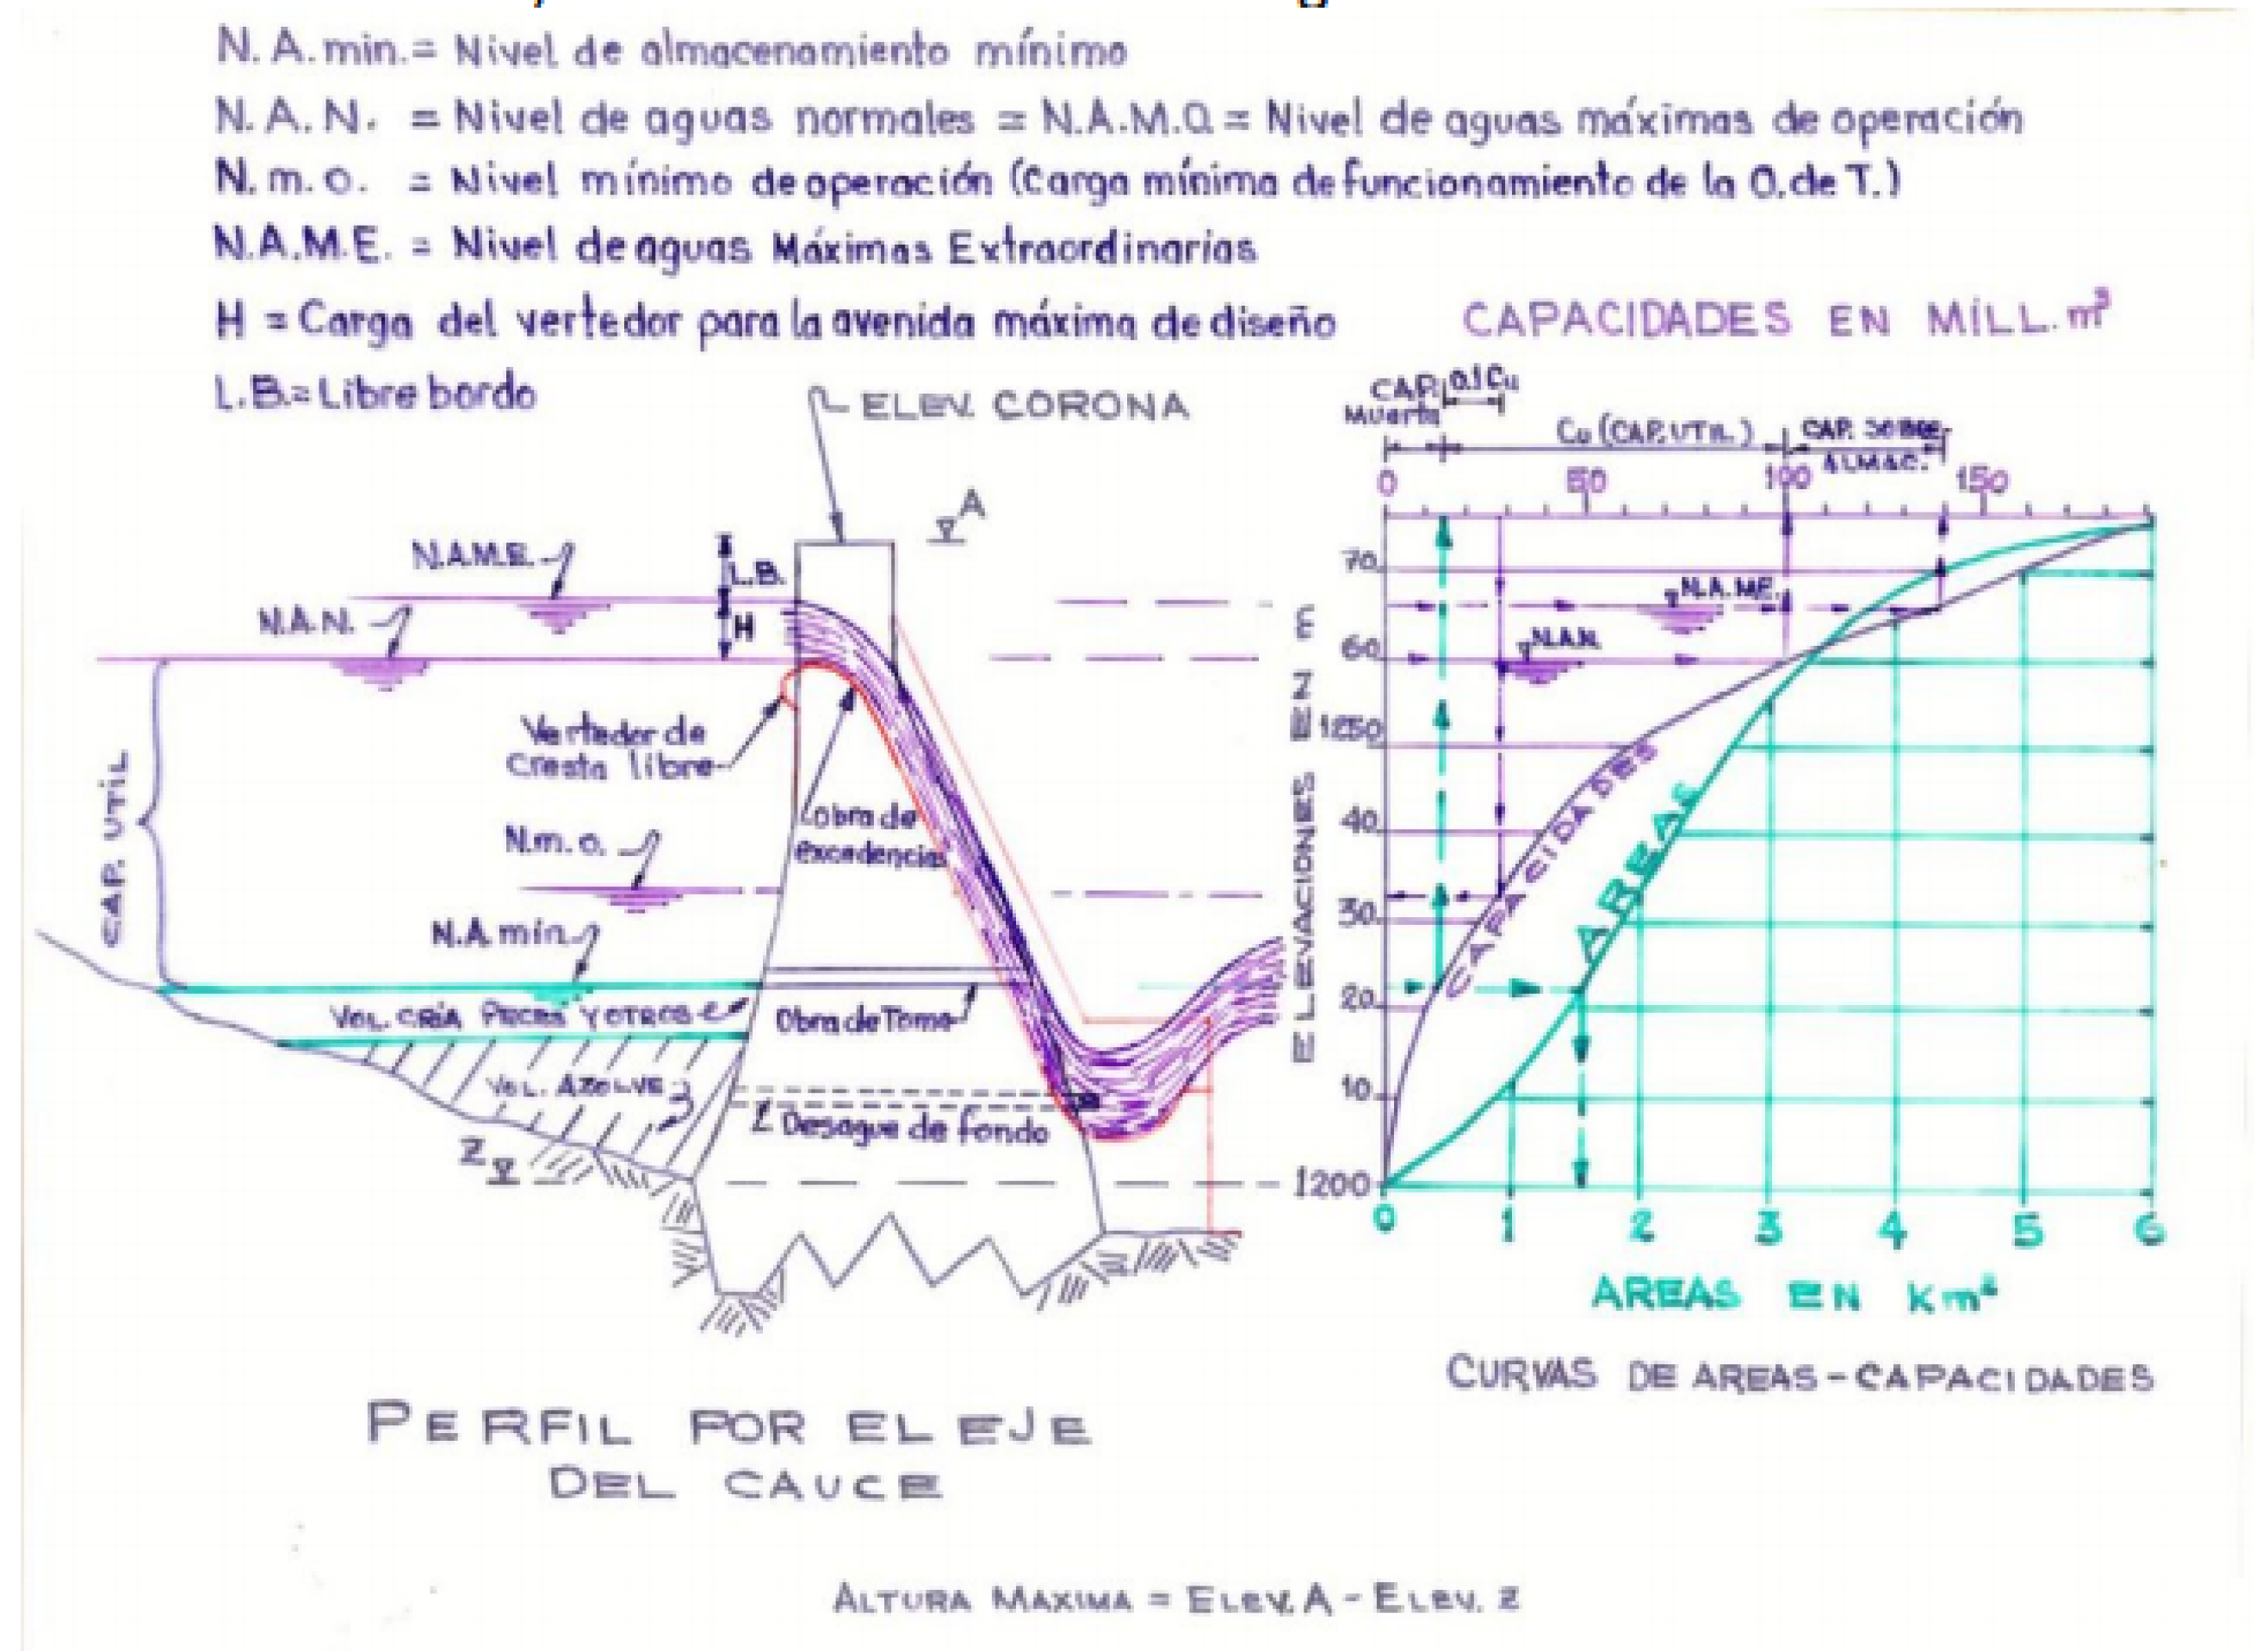
\includegraphics[width=0.5\textwidth]{fii27.png}}
			            \caption{Niveles y capacidades de almacenamiento en una presa.}
			            \label{fii27}
		            \end{figure}
		      \item \textbf{La Capacidad Útil \textbf{(Cu)}}, es el volumen de almacenamiento que representa la
		            diferencia que se tiene en un almacenamiento entre la Capacidad Total y la Capacidad
		            Muerta, este volumen queda conformado por el que se ubica entre los Niveles de
		            Aguas Normales (N.A.N.) y el Nivel de Aguas mínimo (N.A.mín.), y se integra con el
		            volumen útil que se deja para satisfacer lo beneficios que se presentan aguas abajo del
		            almacenamiento, así como el volumen de pérdidas por evaporación y de infiltración.
		      \item \textbf{La capacidad de sobre almacenamiento} es el volumen temporal del
		            almacenamiento que queda por arriba del vertedor de demasías y que se encuentra
		            comprendido entre el Nivel de Aguas Normales (N.A.N.) hasta el Nivel de Aguas
		            Máximas Extraordinarias (N.A.M.E.), esta capacidad en el vaso es de un
		            almacenamiento temporal, en tanto es desalojada por la obra de excedencias cuando
		            esta es de descarga libre, cuando esta descarga se controla por medio de compuertas
		            es un almacenamiento que se maneja acorde a los beneficios y finalidad del
		            almacenamiento, que entre otros es el control de avenidas.
		      \item \textbf{El Nivel de Aguas Máximas Extraordinarias \textbf{(N.A.M.E.)}} es la cota virtual del
		            almacenamiento que define el diseño de la obra de excedencias y que permite el paso
		            de la avenida máxima que llega al vaso y que es desalojada por esta estructura.
		      \item \textbf{El Nivel mínimo de operación \textbf{(N.m.o.)}} es la cota del almacenamiento a partir
		            del cual el gasto normal para riego es extraído en forma controlada a través de la Obra
		            de Toma y es el nivel que permite el diseño de esta estructura. Cuando se refiere el
		            N.m.o. a la operación de una máquina hidráulica (Planta de Bombeo o Instalaciones de
		            Turbinas generadoras de energía), esta cota es vital ya que es la que permite
		            operarlas, ya que si se da esta por debajo de ella se presentara un fenómeno que
		            destruiría a la máquina hidráulica, esto es el fenómeno de cavitación.
	      \end{enumerate}
	\item \textbf{Altura Máxima de la cortina:} La altura de la presa es determinada mediante la diferencia de elevaciones entre
	      la cota de la corona en la presa y la cota del fondo del cauce en la sección máxima de
	      la cortina. La elevación de la corona se obtiene con el N.A.M.E. adicionando el Libre
	      Bordo (L.B.) que es una altura de seguridad ante la presencia del oleaje que bajo la
	      acción del viento en el vaso de almacenamiento se presenta, complementado con un
	      factor de seguridad por el efecto de rompimiento de la ola al chocar con el paramento
	      mojado.
\end{enumerate}

\subsection{Obra de Retención o cortina}

\begin{definition}[Obra de retención]
	La obra de retención o cortina es la estructura del sistema de almacenamiento,
	mediante la cual se cierra artificialmente un vaso o valle natural en una cuenca de
	drenaje con el objeto de provocar un embalse. La función de esta es retener las aguas para
	formar el vaso de almacenamiento y regular los escurrimientos del cauce.
\end{definition}

Propósitos y características de una obra de retención o cortinas:
Los propósitos de una cortina son el almacenar agua para utilizarla en diferentes
usos:

\begin{itemize}
	\item  Riego
	\item  Generación de energía
	\item  Control de avenidas
	\item  Usos domésticos
	\item  Abrevadero y cría de peces
	\item  Recreación
\end{itemize}

Las características de una cortina deben brindar condiciones para que sea
Estable e Impermeable. Sus formas de clasificación de las cortinas:
\begin{enumerate}
	\item Por su uso
	      \begin{enumerate}
		      \item Generación de energía
		      \item Agua potable
		      \item Control de avenidas
		      \item Riego
	      \end{enumerate}
	\item Por su altura, están en la tabla \ref{tab17}
	      \begin{table}[h!]
		      \centering
		      \begin{tabular}{|c|c|c|c|}
			      \hline
			                & Según Torres H.        & Según U.S.B.R. & Según I.C.O.L.D. \\ \hline
			      Bajas:    & $H < 30 m$             & $H \leq 30 m$  & $H \geq 15 m$    \\ \hline
			      Medianas: & $30 m  \leq H < 100 m$ & $H \leq 90 m$  &                  \\ \hline
			      Altas:    & $H \geq 100 m$         & $H > 90 m$     & $H > 15 m$       \\ \hline
		      \end{tabular}
		      \caption{Altura de cortinas}
		      \label{tab17}
	      \end{table}
	      pueden ser Vertedoras o No vertedoras
	\item Por su funcionamiento hidráulico
	      pueden ser Vertedoras o No vertedoras
	\item Por el tipo de construcción y materiales que le constituyen.
	      pueden ser \textbf{Rígidas (Concreto
		      o Mampostería)} pero también \textbf{Flexibles ( Tierra, Enrocamiento, Materiales graduados, Madera y/o Mixtas)}
	\item Por los esfuerzos que transmiten.
	      \begin{enumerate}
		      \item En planos verticales (hacia la cimentación): Gravedad ó Machones y contrafuertes.
		      \item En planos horizontales (hacia las laderas): Arco ó Bóveda
		      \item En planos combinados (Horizontales y verticales): Arco gravedad
	      \end{enumerate}
\end{enumerate}

\subsubsection{Clasificación SRH de cortinas}
\Schema{-1.4ex}{30ex}
{\schemabox{Cortinas}} { \Schema{-1ex}{12ex}
	{\schemabox{Rígidas vertedoras\\ y no vertedoras}}
	{ \schema
		{\schemabox{Gravedad}}
		{\schemabox{Eje Recto\\ Eje Curvo\\
				Aligeradas}}
		\medskip
		\schema
		{\schemabox{Arco}}
		{\schemabox{Arco Simple\\ Arco Gravedad\\
				Bóvedas\\ Arcos Múltiples.}}
		\Schema{0ex}{3.4ex}
		{\schemabox{Diques\\ huecos}}
		{
			\Schema{0ex}{3.4ex}
			{\NudgeSB\schemabox{Losa y contrafuerte\\ Machones de cabeza\\ Bóvedas Múltiples}}
			{\schemabox{Redonda\\ Diamante}}
		}
	}
	\Schema{-1ex}{5ex}
	{\schemabox{Flexibles}}
	{
		\vskip1ex\schemabox{Materiales graduados}
		\medskip
		\schemabox{Tierras (Homogéneas)}
		\medskip
		\schema
		{\schemabox{Enrocamiento}}
		{\schemabox{Con Corazón Impermeable\\ Con Membrana Impermeable}}
	}
	\Schema{-1ex}{5ex}
	{\schemabox{Mixtas}}
	{
		\schemabox{Madera y enrocamiento}
		\medskip\schemabox{Madera y Concreto}
		\medskip
		\schemabox{Concreto y Fierro}}
	\Schema{-1ex}{5ex}
	{\schemabox{Compuertas}}
	{
		\schemabox{Diversos Materiales en diversas secciones}}}

\subsection{Diversos tipos de presas}

\subsubsection{Cortinas o presas de gravedad:}
Es una estructura sólida de algún material rígido que se diseña y se
proporciona, para asegurar su estabilidad contra los efectos de todas las fuerzas que
se le impongan a partir del empuje del agua. Se usa la mampostería: en presas pequeñas $(H<30 m)$, este material se
conforma con piedra (o roca) junteada con mortero de cemento (mezcla cemento arena), debidamente colocada.

Otra opción, se puede usar Concreto simple, material que se conforma con una mezcla de arena, grava, cemento y agua;

La tercera opción es Concreto ciclópeo: piedra agregada en un 30\% sobre el concreto simple. Finalmente se puede optar por usar el colcreto: piedra rellenada con mortero coloidal, ya sea inyectada o
colocada por gravedad. Se le conoce como mampostería inyectada.

\subsubsection{Cortinas o presas de arco:} Es una estructura sólida construida normalmente de concreto de gran esbeltez, en forma de arco, la que, a través del efecto de este, hace que los esfuerzos originados en el empuje del agua, todos ellos vayan a dar a las laderas.

\begin{figure}[h!]
	\centerline{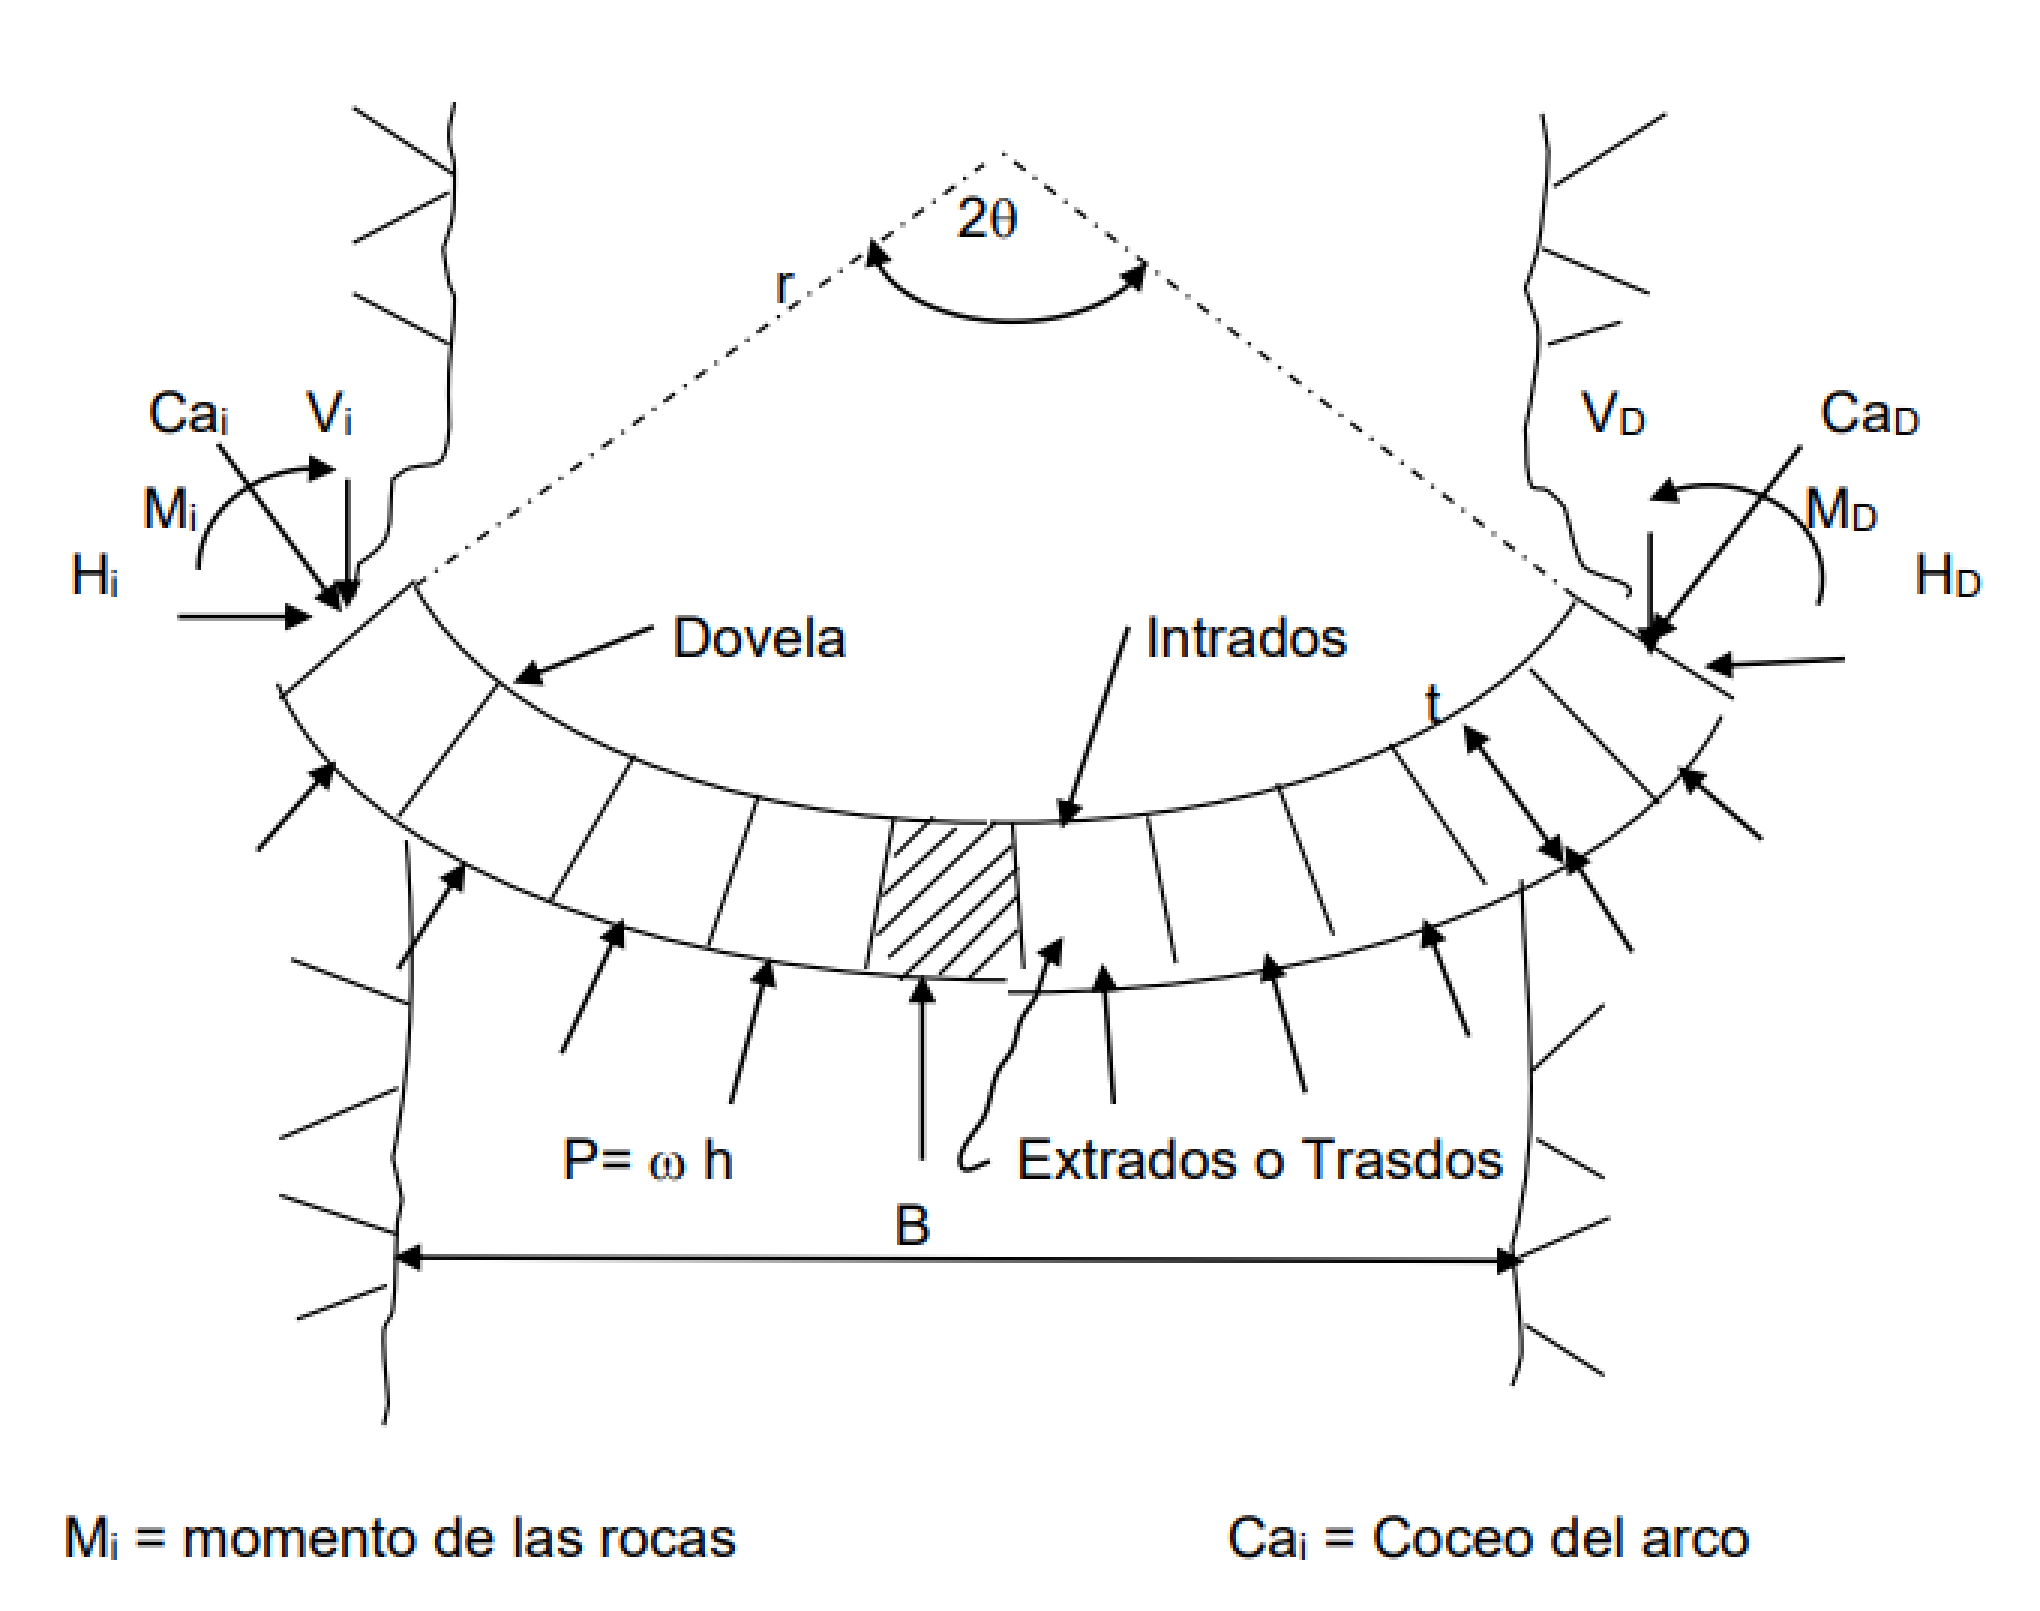
\includegraphics[width=0.5\textwidth]{fii28.png}}
	\caption{ Planta esquemática de Presa de arco.}
	\label{fii28}
\end{figure}

El Arco óptimo se tiene con: $2\theta = 133^{\circ} 34'$; Para minimizar material, los arcos se pueden encontrar entre: $100^{\circ} \leq  2\theta \leq  140^{\circ}$P
Para cañones de: $B \leq \frac{H}{3} \longrightarrow$ Presa de arco
Para cañones de: $B \geq 2.5H \longrightarrow$ Presas de Arco-Gravedad.
\begin{figure}[h!]
	\centerline{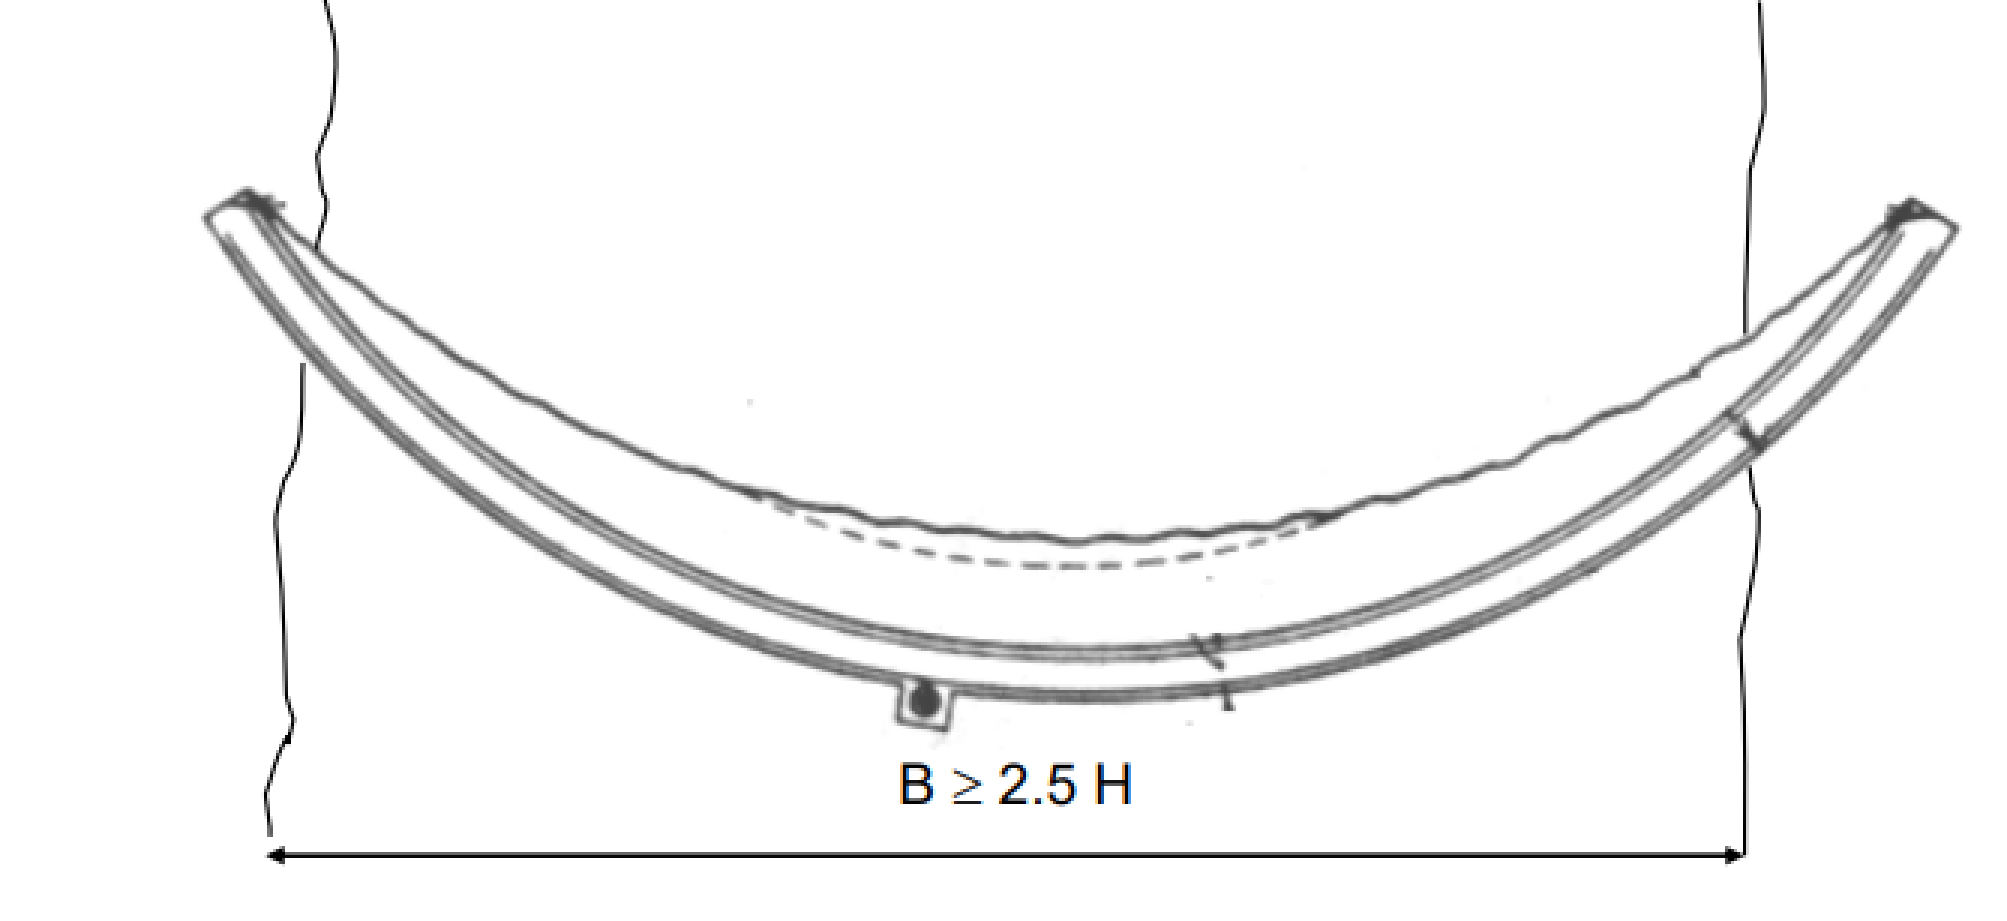
\includegraphics[width=0.5\textwidth]{fii29.png}}
	\caption{Forma en planta de una presa de arco.}
	\label{fii29}
\end{figure}
\textbf{Por su geometría:} Radio Constante o de centro constante y por Radio variable o ángulo constante
\begin{figure}[h!]
	\centerline{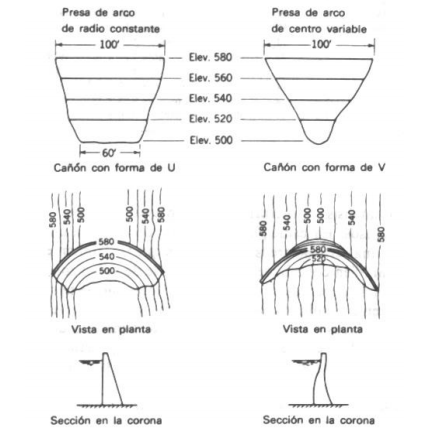
\includegraphics[width=0.5\textwidth]{fii30.png}}
	\caption{Clasificación de presas de arco.}
	\label{fii30}
\end{figure}
\textbf{Por su simetría respecto al eje del cañón:} Simétricas y Asimétricas

%%%%%%%%%%%%%%%%%%%%% Asimetría en presas de arco img


\textbf{Por su espesor:} Arco delgado $( \frac{r}{t\geq 5} )$, Arco grueso $( \frac{r}{t < 5})$, Espesor constante y Espesor variable.

\subsubsection{Cortina o presa de diques huecos:} Este tipo de presas se caracteriza por tener una membrana inclinada que
transmite la carga de agua a una serie de contrafuertes (o machones) en ángulos rectos al eje de la presa.
\begin{figure}[h!]
	\centerline{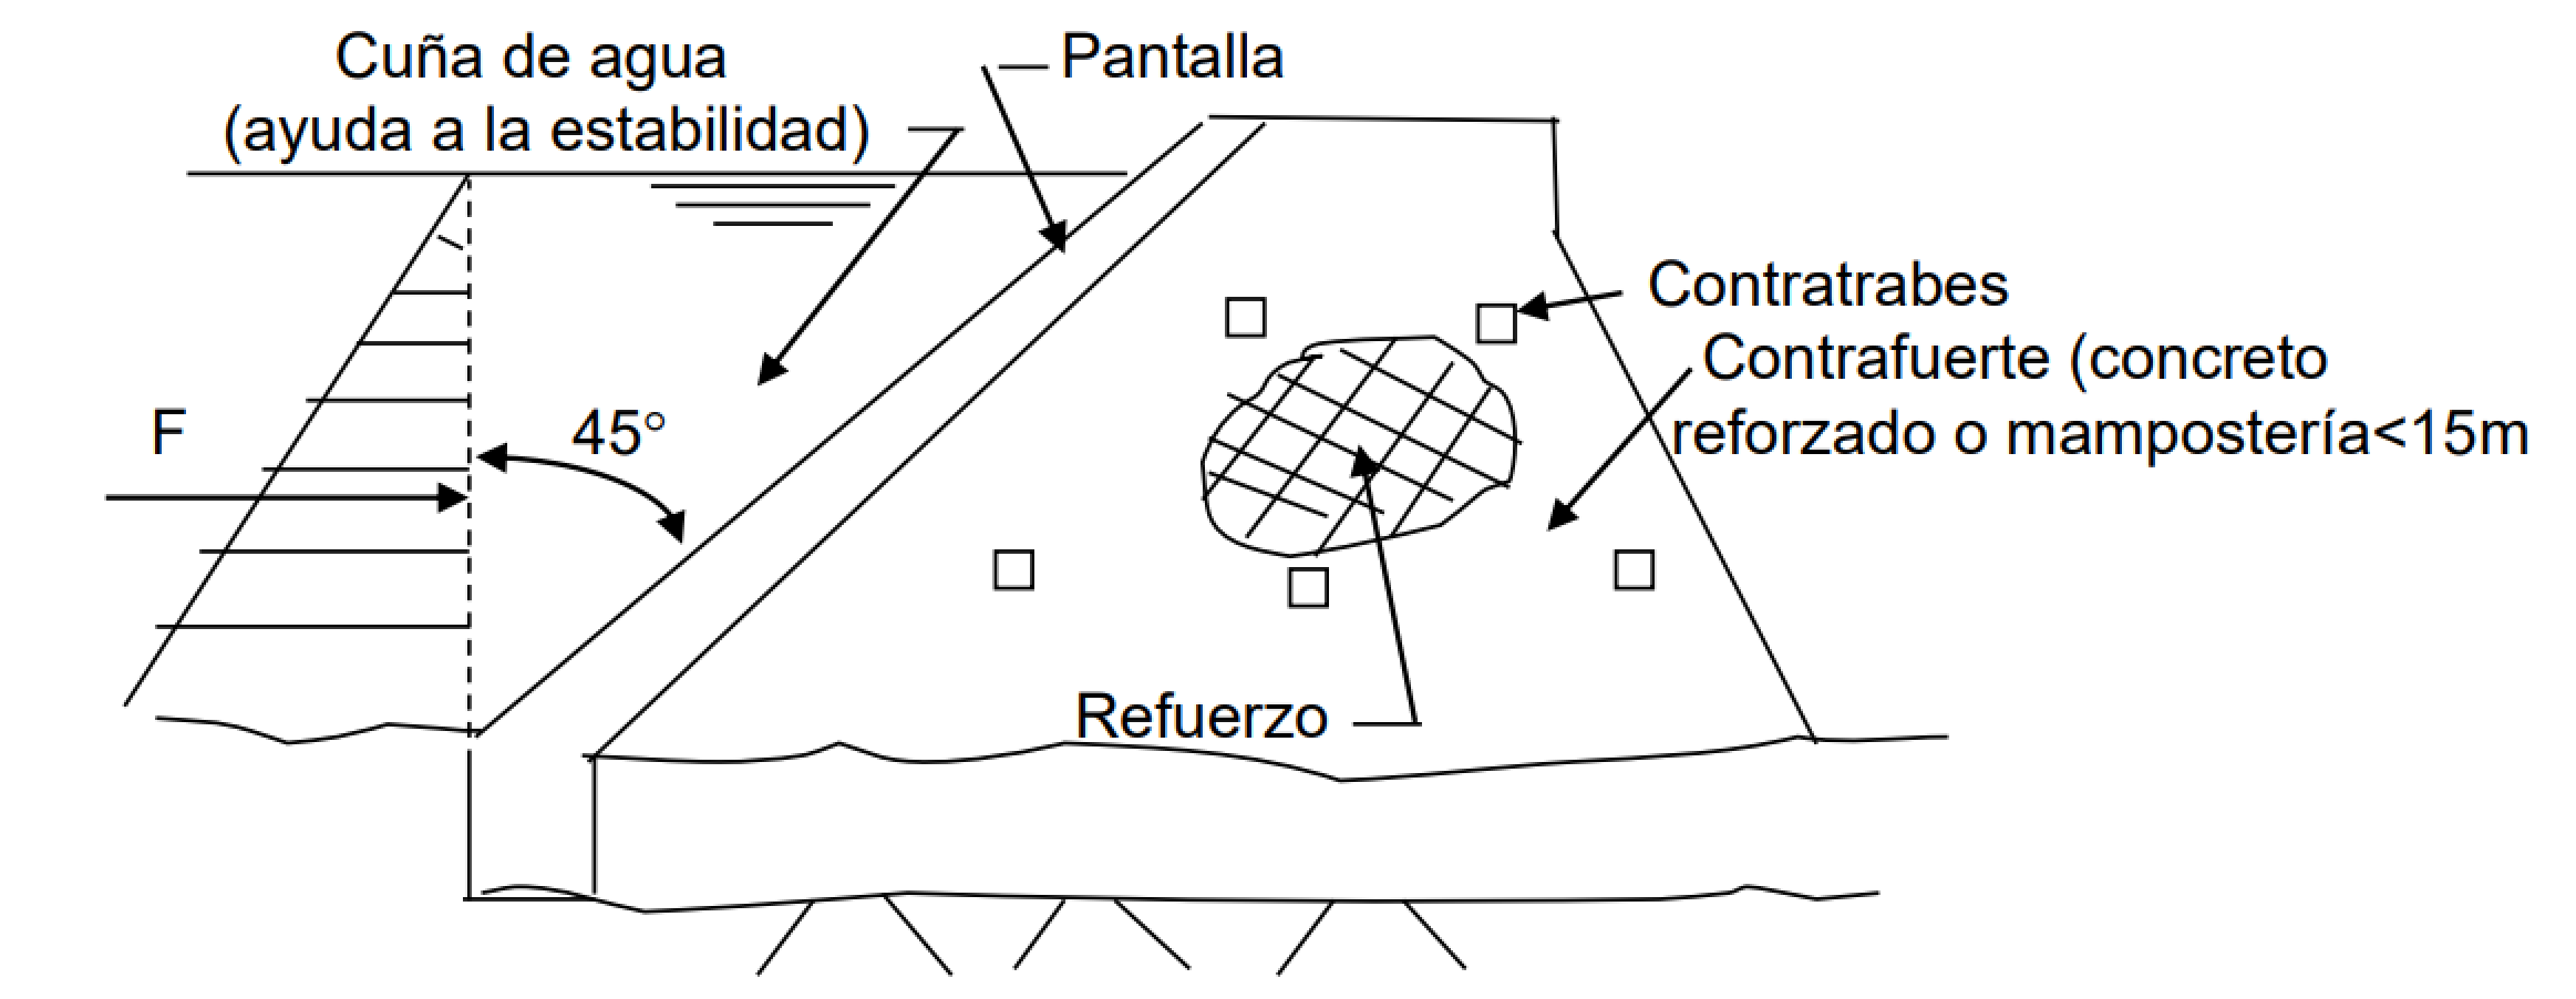
\includegraphics[width=0.5\textwidth]{fii31.png}}
	\caption{Esquema de Presa de diques huecos tipo Ambursen.}
	\label{fii31}
\end{figure}
Nils Ambursen construyó en 1903 la primera presa de machones y losa de concreto.

\begin{figure}[h!]
	\centerline{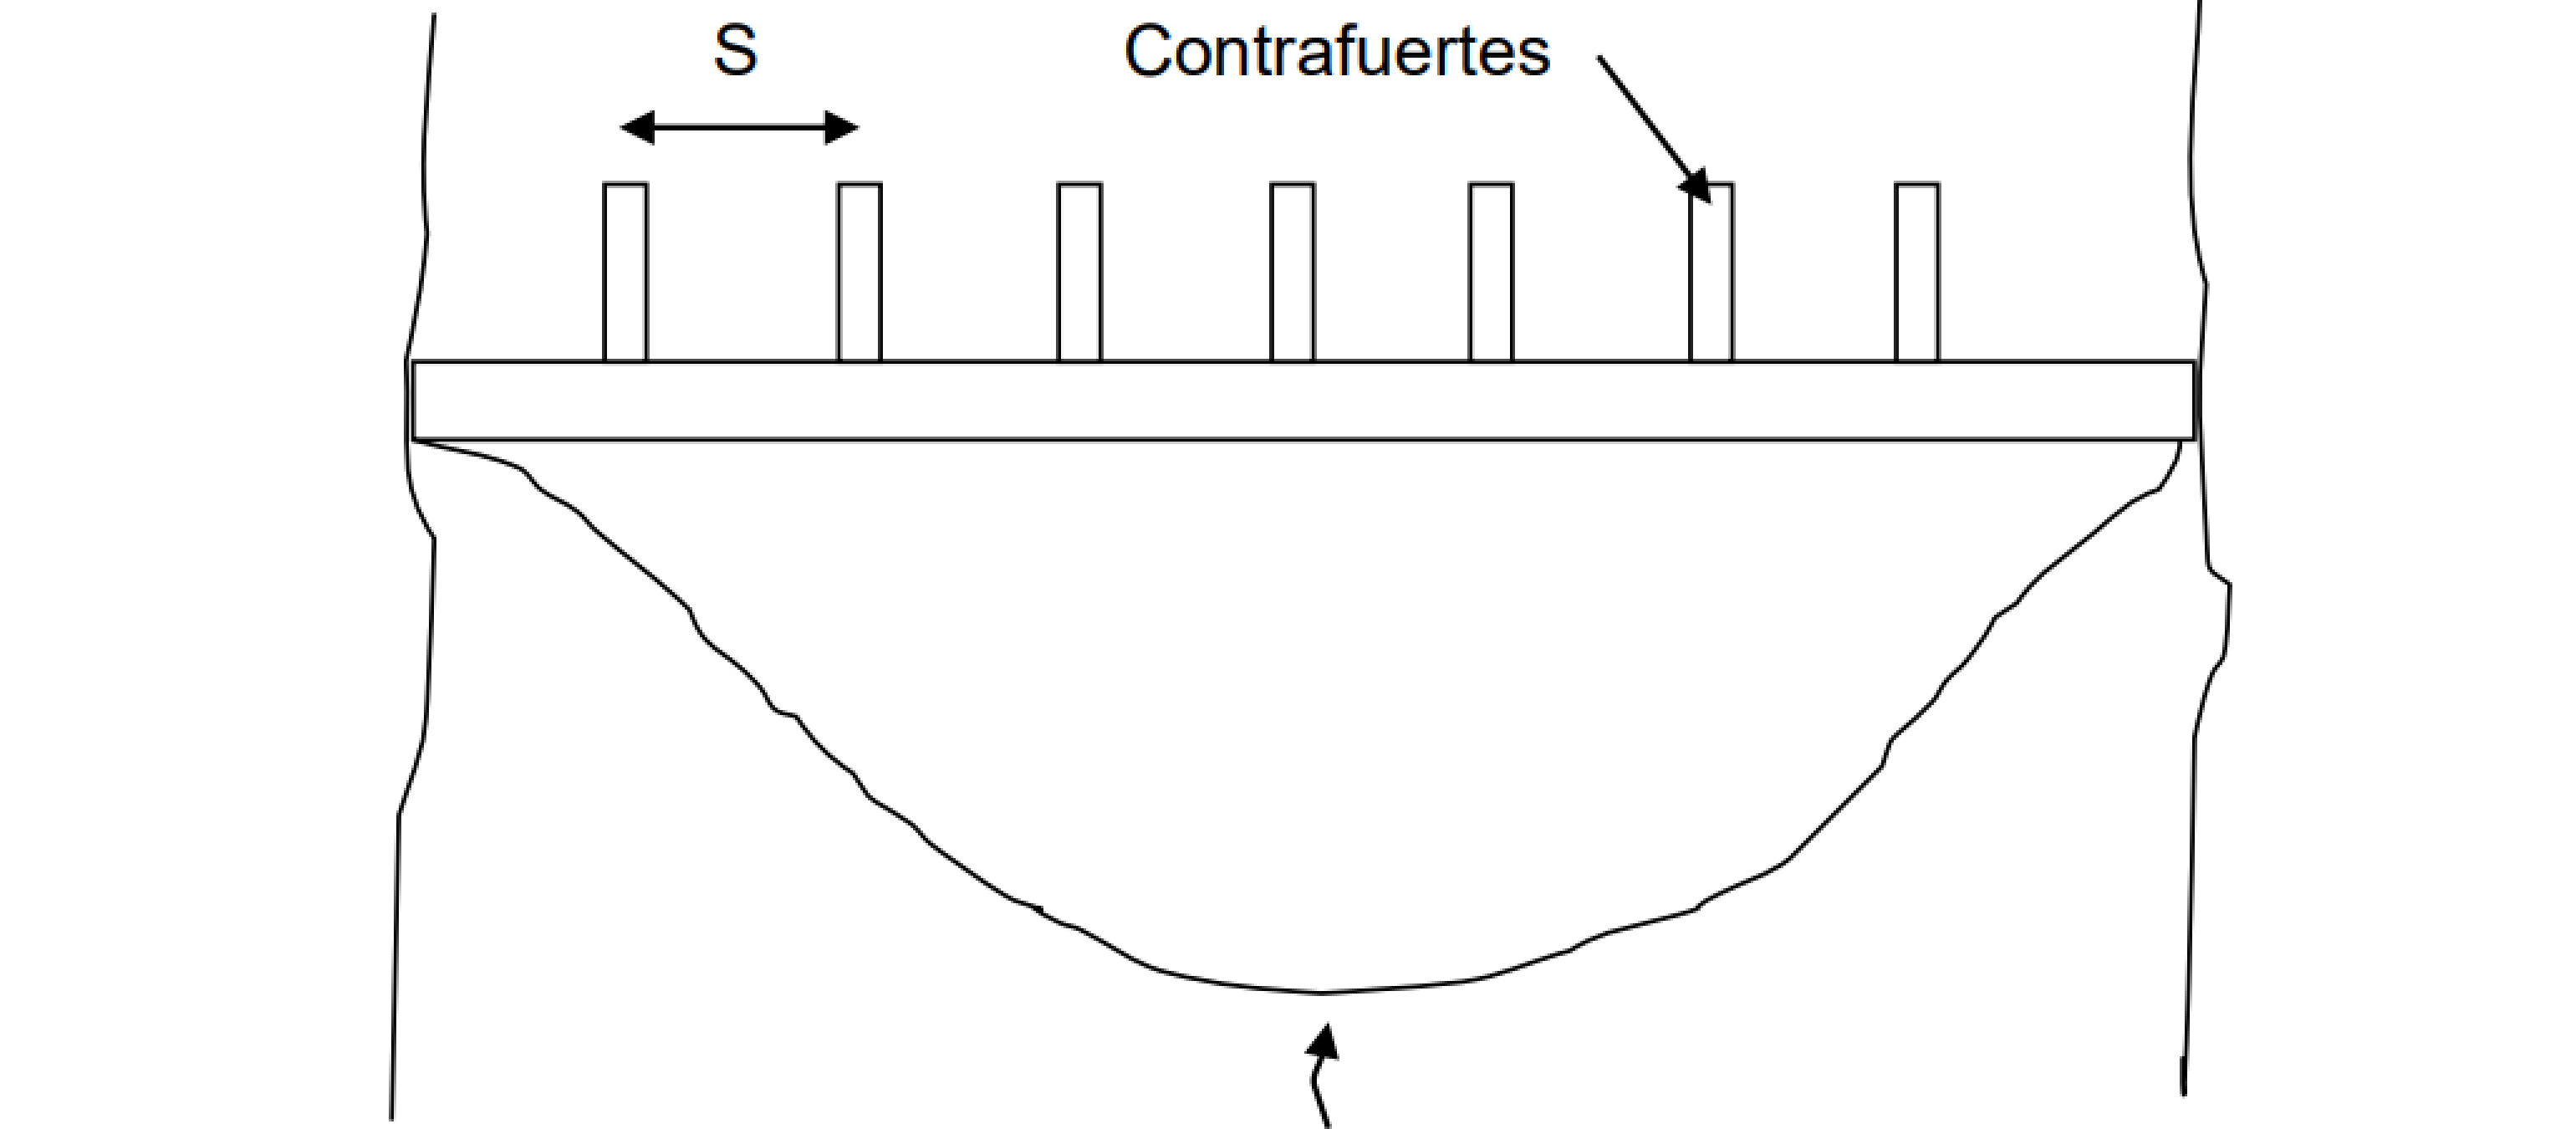
\includegraphics[width=0.5\textwidth]{fii32.png}}
	\caption{ Planta Esquemática genérica de Presa de diques huecos.}
	\label{fii32}
\end{figure}

Clasificación de Presas de diques huecos:

\begin{enumerate}[noitemsep]
	\item Pantalla y contrafuertes (Ambursen), Separación del contrafuerte:
	      $ S= 5 m \longrightarrow H= 15 m$
	      $S=15m \longrightarrow H = 50 m$
	\item Arcos múltiples $( 2\theta = 180^{\circ}, 190^{\circ})$
	\item Machones de cabeza : En T, Redonda, Diamante y Machones celulares
	\item Bóvedas múltiples:
	      \begin{figure}[h!]
		      \centerline{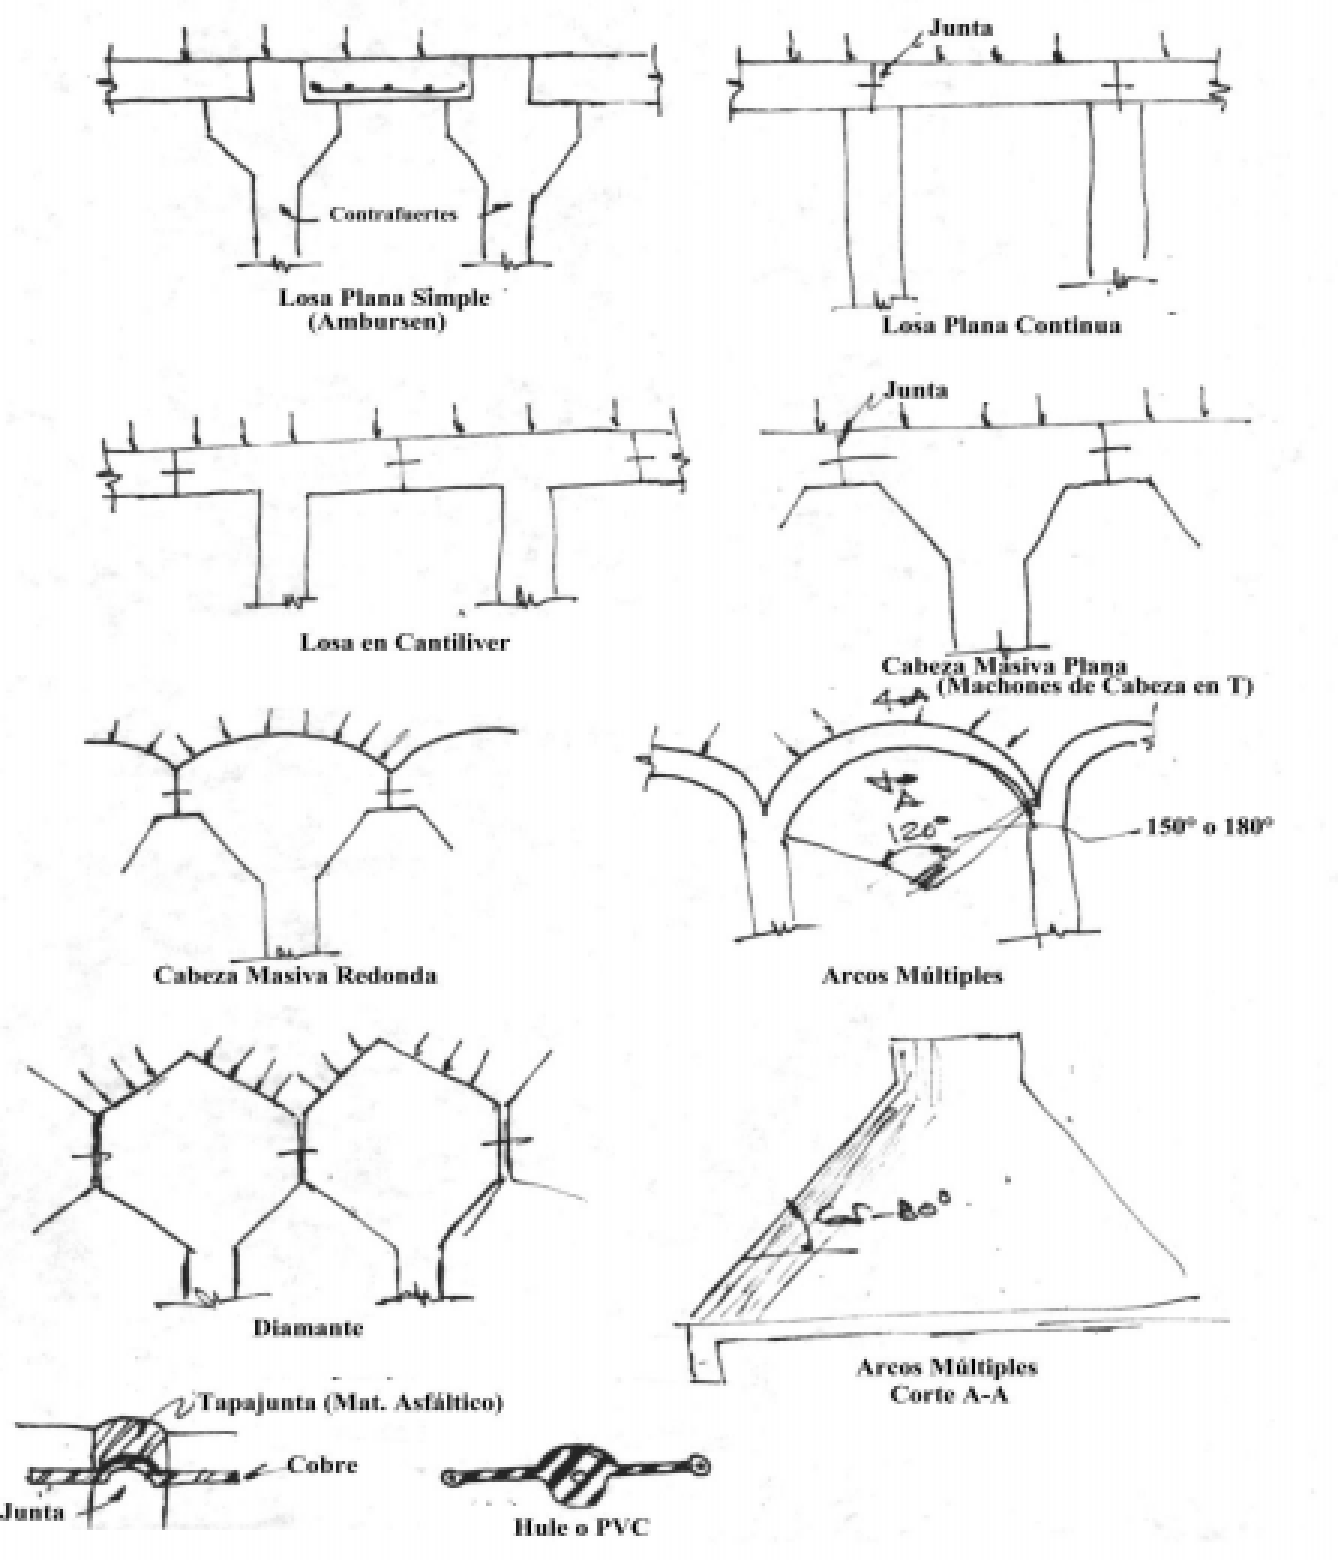
\includegraphics[width=0.5\textwidth]{fii33.png}}
		      \caption{Diferentes plantas esquemáticas de presas de diques huecos.}
		      \label{fii33}
	      \end{figure}
	      \begin{figure}[h!]
		      \centerline{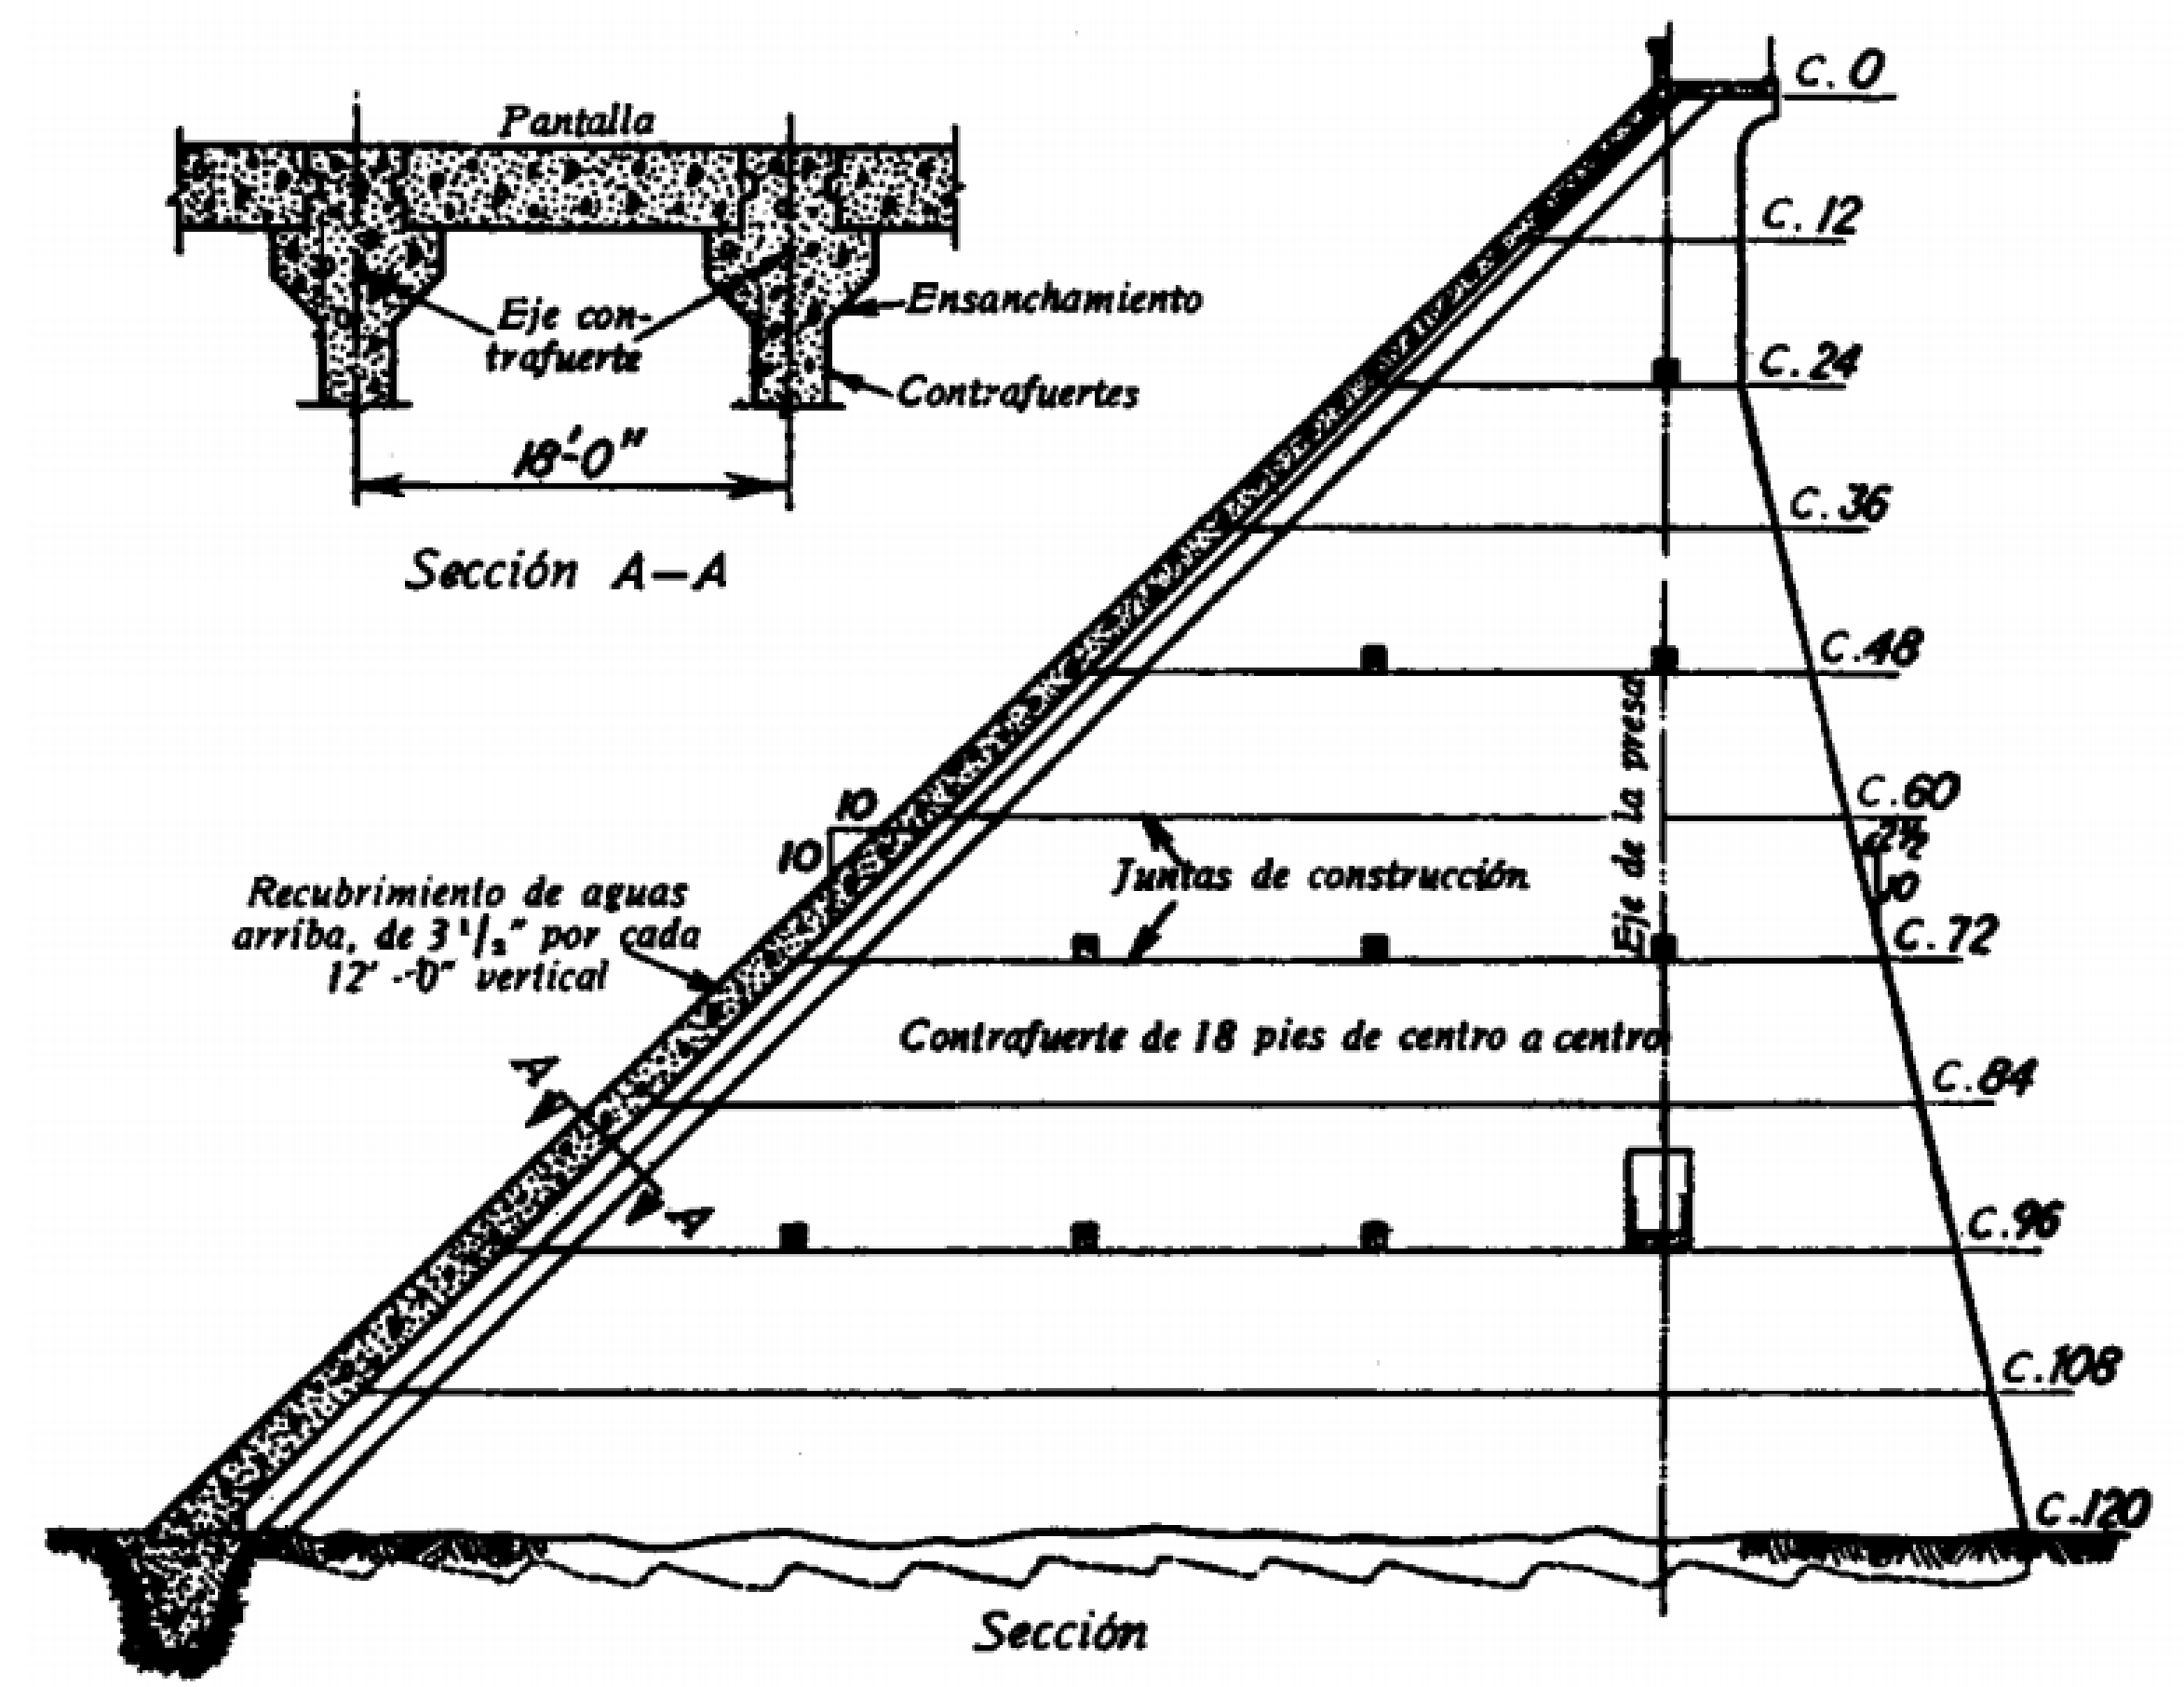
\includegraphics[width=0.5\textwidth]{fii34.png}}
		      \caption{Perfil esquemático de Presa de diques huecos tipo losa y contrafuertes.}
		      \label{fii34}
	      \end{figure}
	      \begin{figure}[h!]
		      \centerline{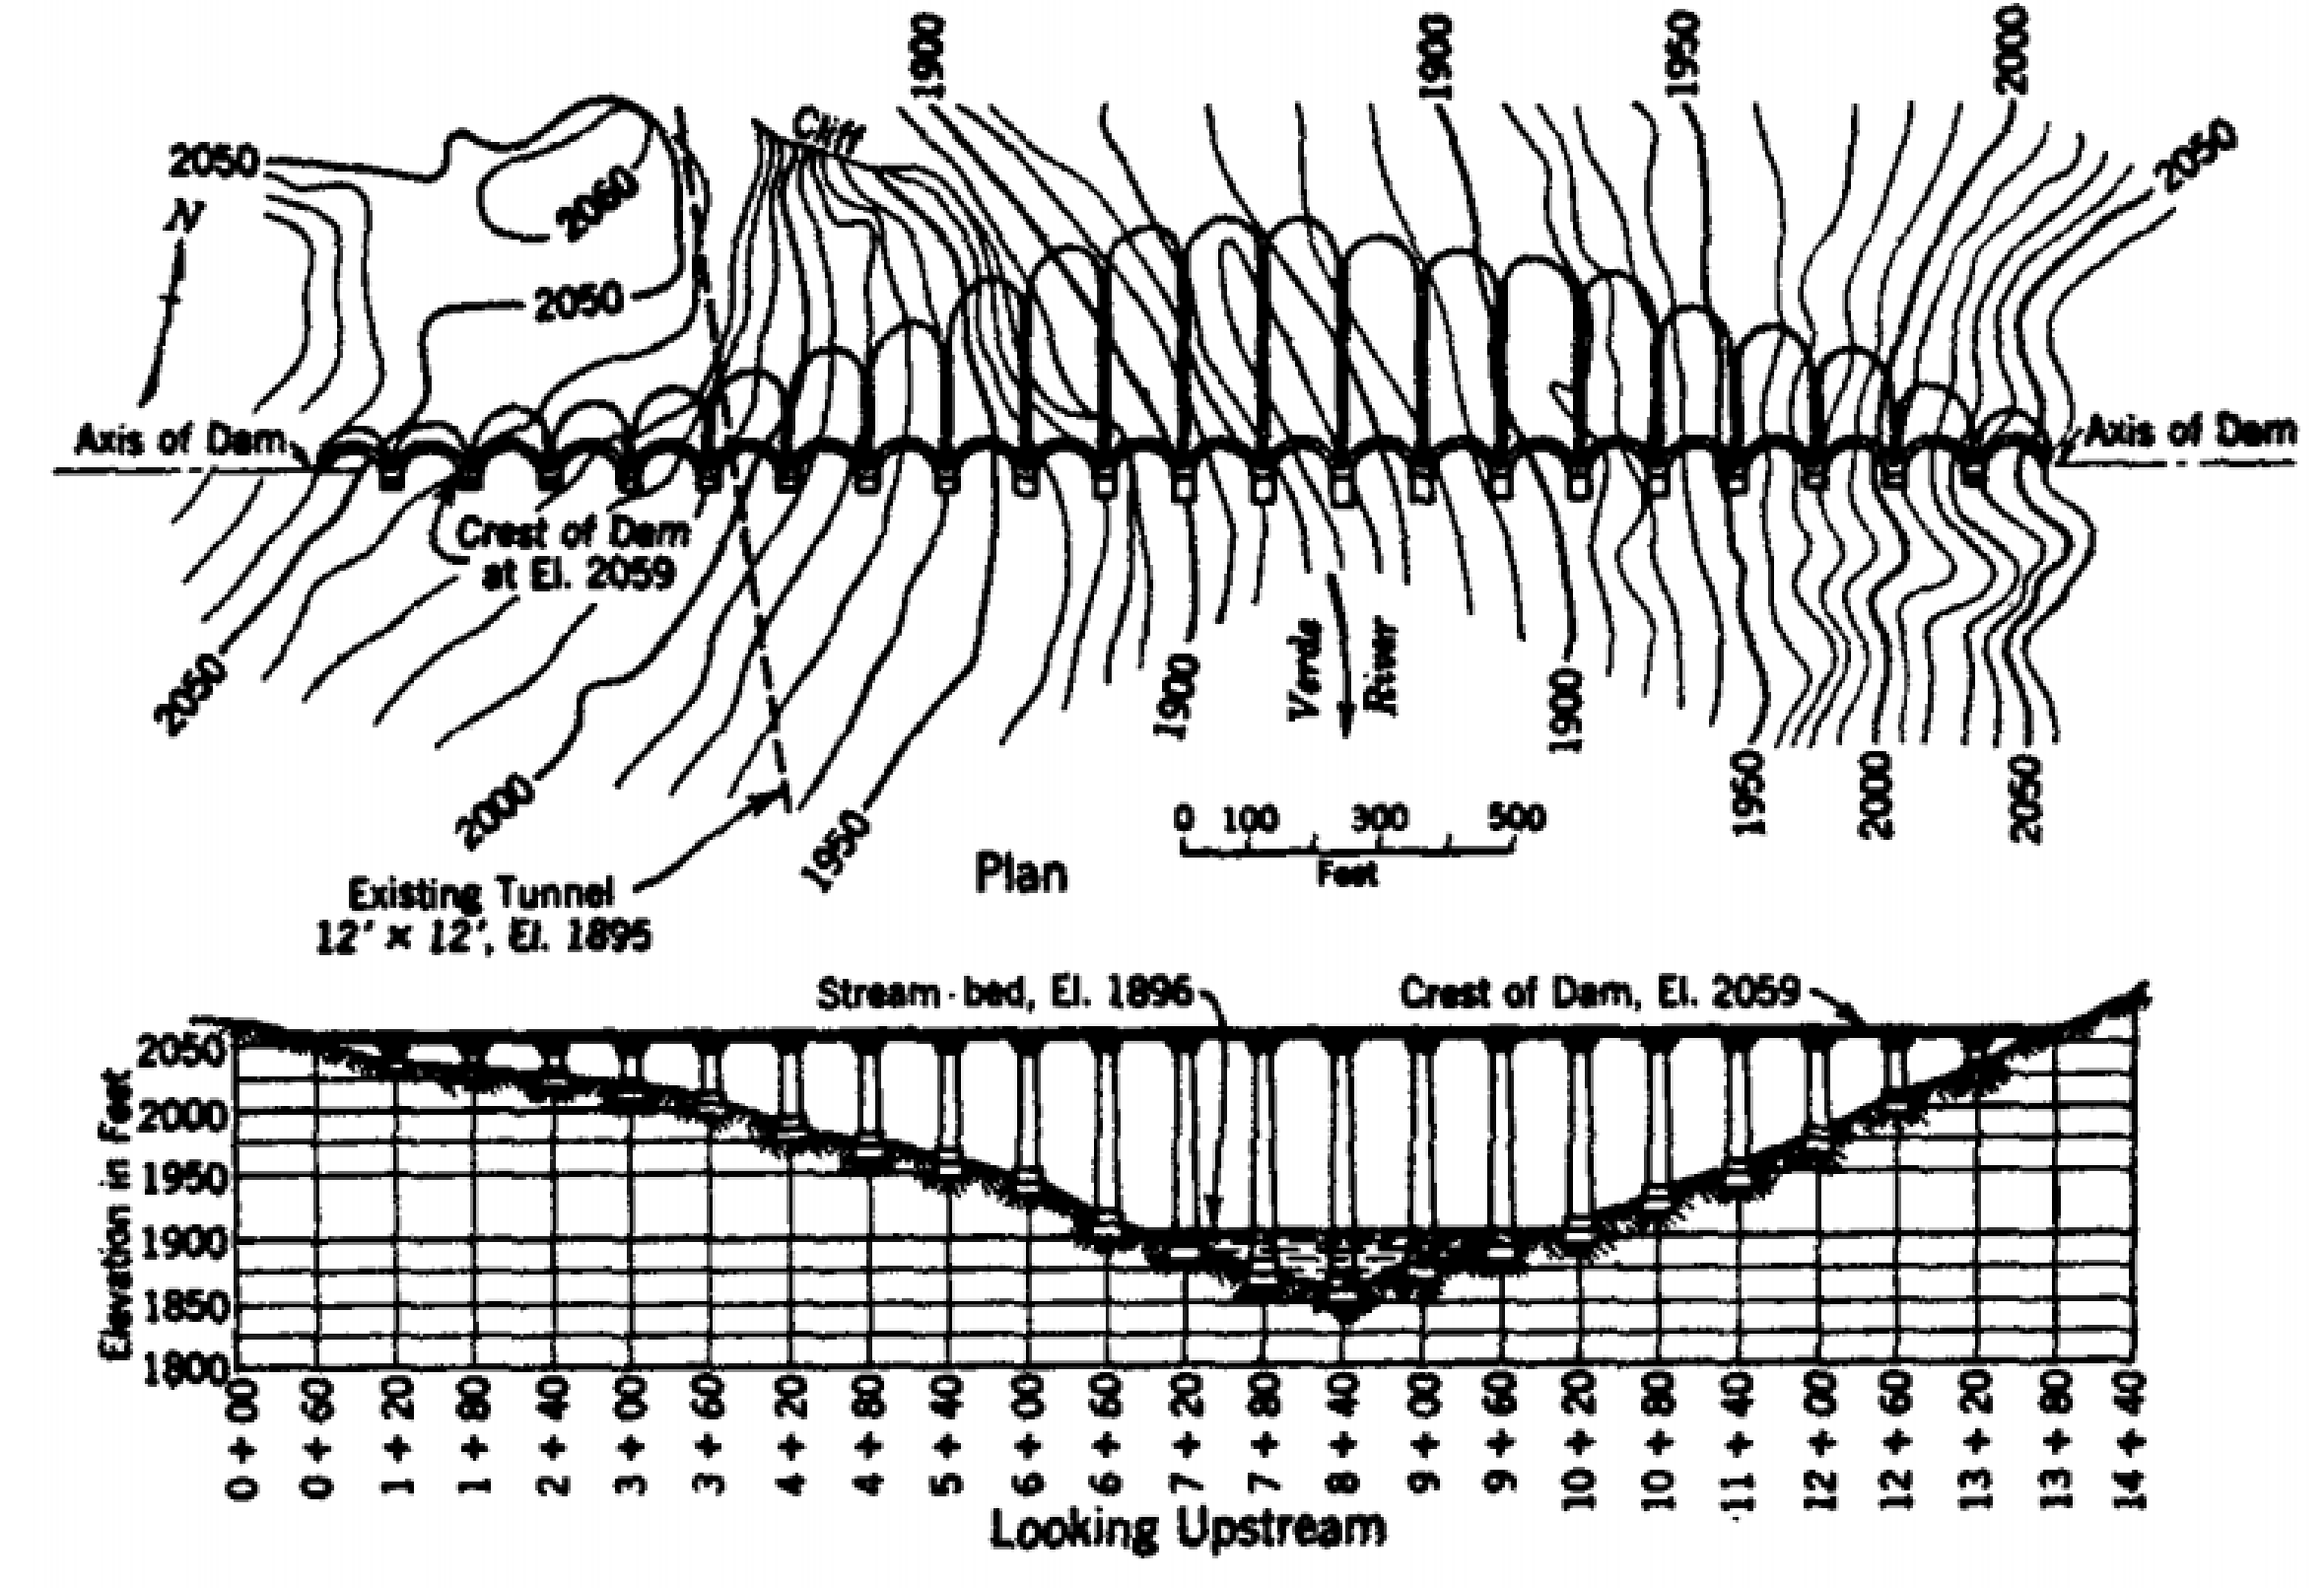
\includegraphics[width=0.5\textwidth]{fii35.png}}
		      \caption{Planta y perfil por el eje de Presa de diques huecos tipo arcos
			      múltiples.}
		      \label{fii35}
	      \end{figure}
	      \begin{figure}[h!]
		      \centerline{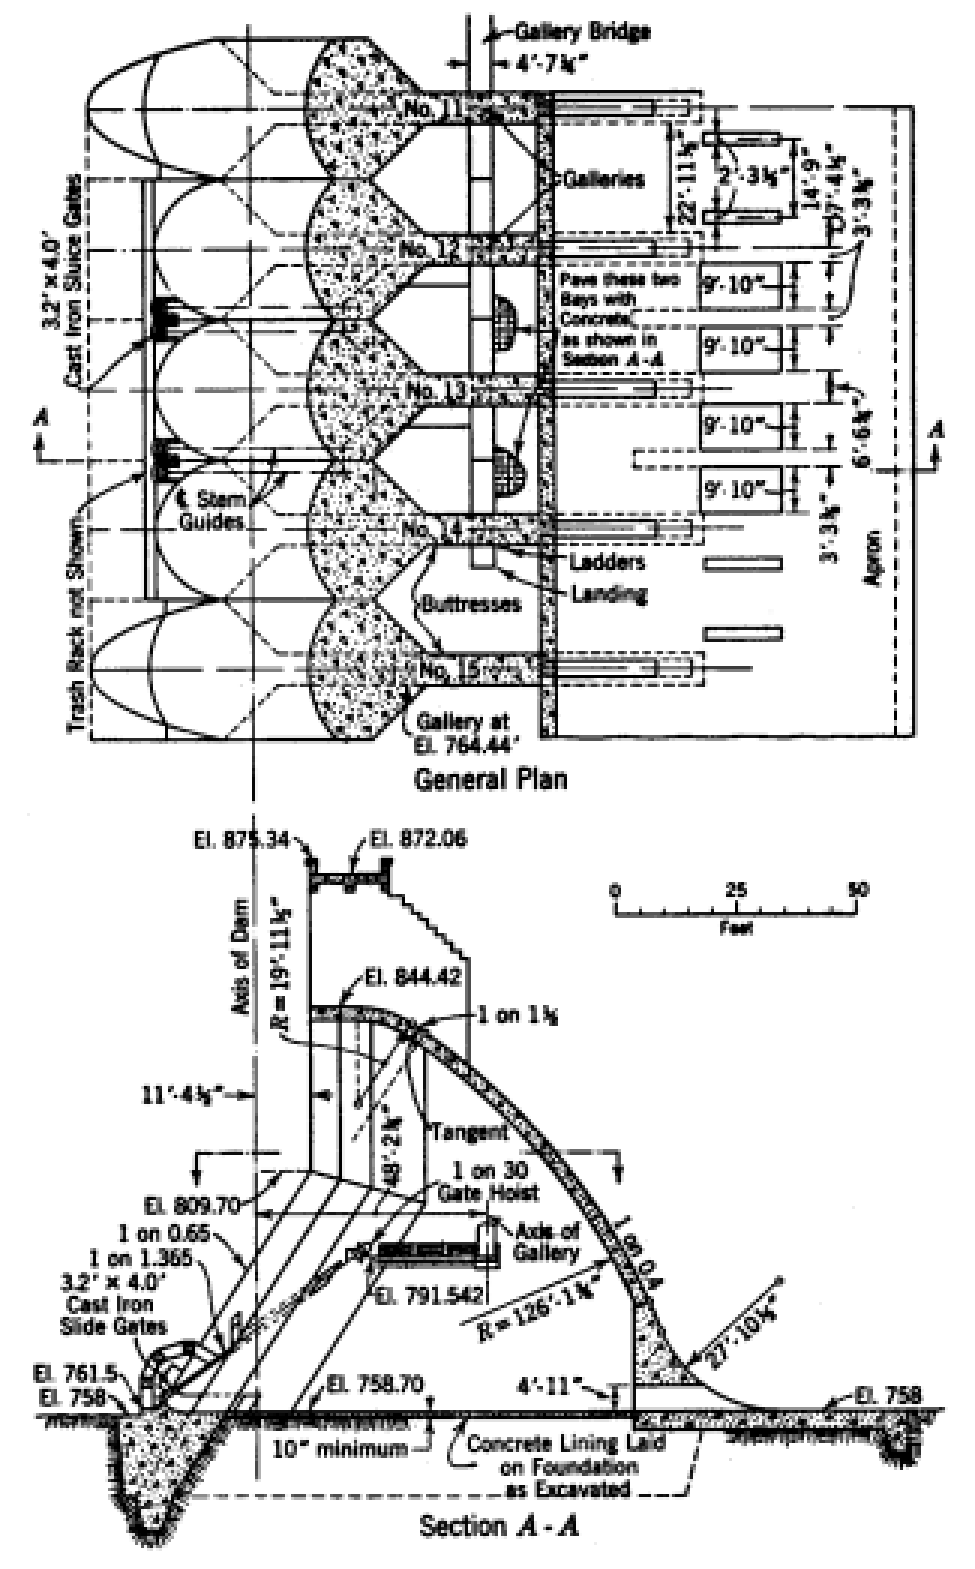
\includegraphics[width=0.5\textwidth]{fii36.png}}
		      \caption{Planta y Perfil de Presa de diques huecos tipo machones de cabeza
			      redonda.}
		      \label{fii36}
	      \end{figure}
\end{enumerate}

\subsubsection{Cortinas de materiales flexibles}

\subsubsection{Presas de tierra}

\begin{definition}[Presas de tierra]
	Una presa de tierra es una estructura formada con materiales naturales
	granulares sin más tratamiento que su colocación debidamente compactados.
\end{definition}

Secciones típicas: las Homogéneas se dividen en presas pequeñas y mixtas. Los materiales graduados se usan para las presas grandes.

\begin{enumerate}[noitemsep]
	\item Presas de tierra de sección homogénea
	      \begin{figure}[h!]
		      \centerline{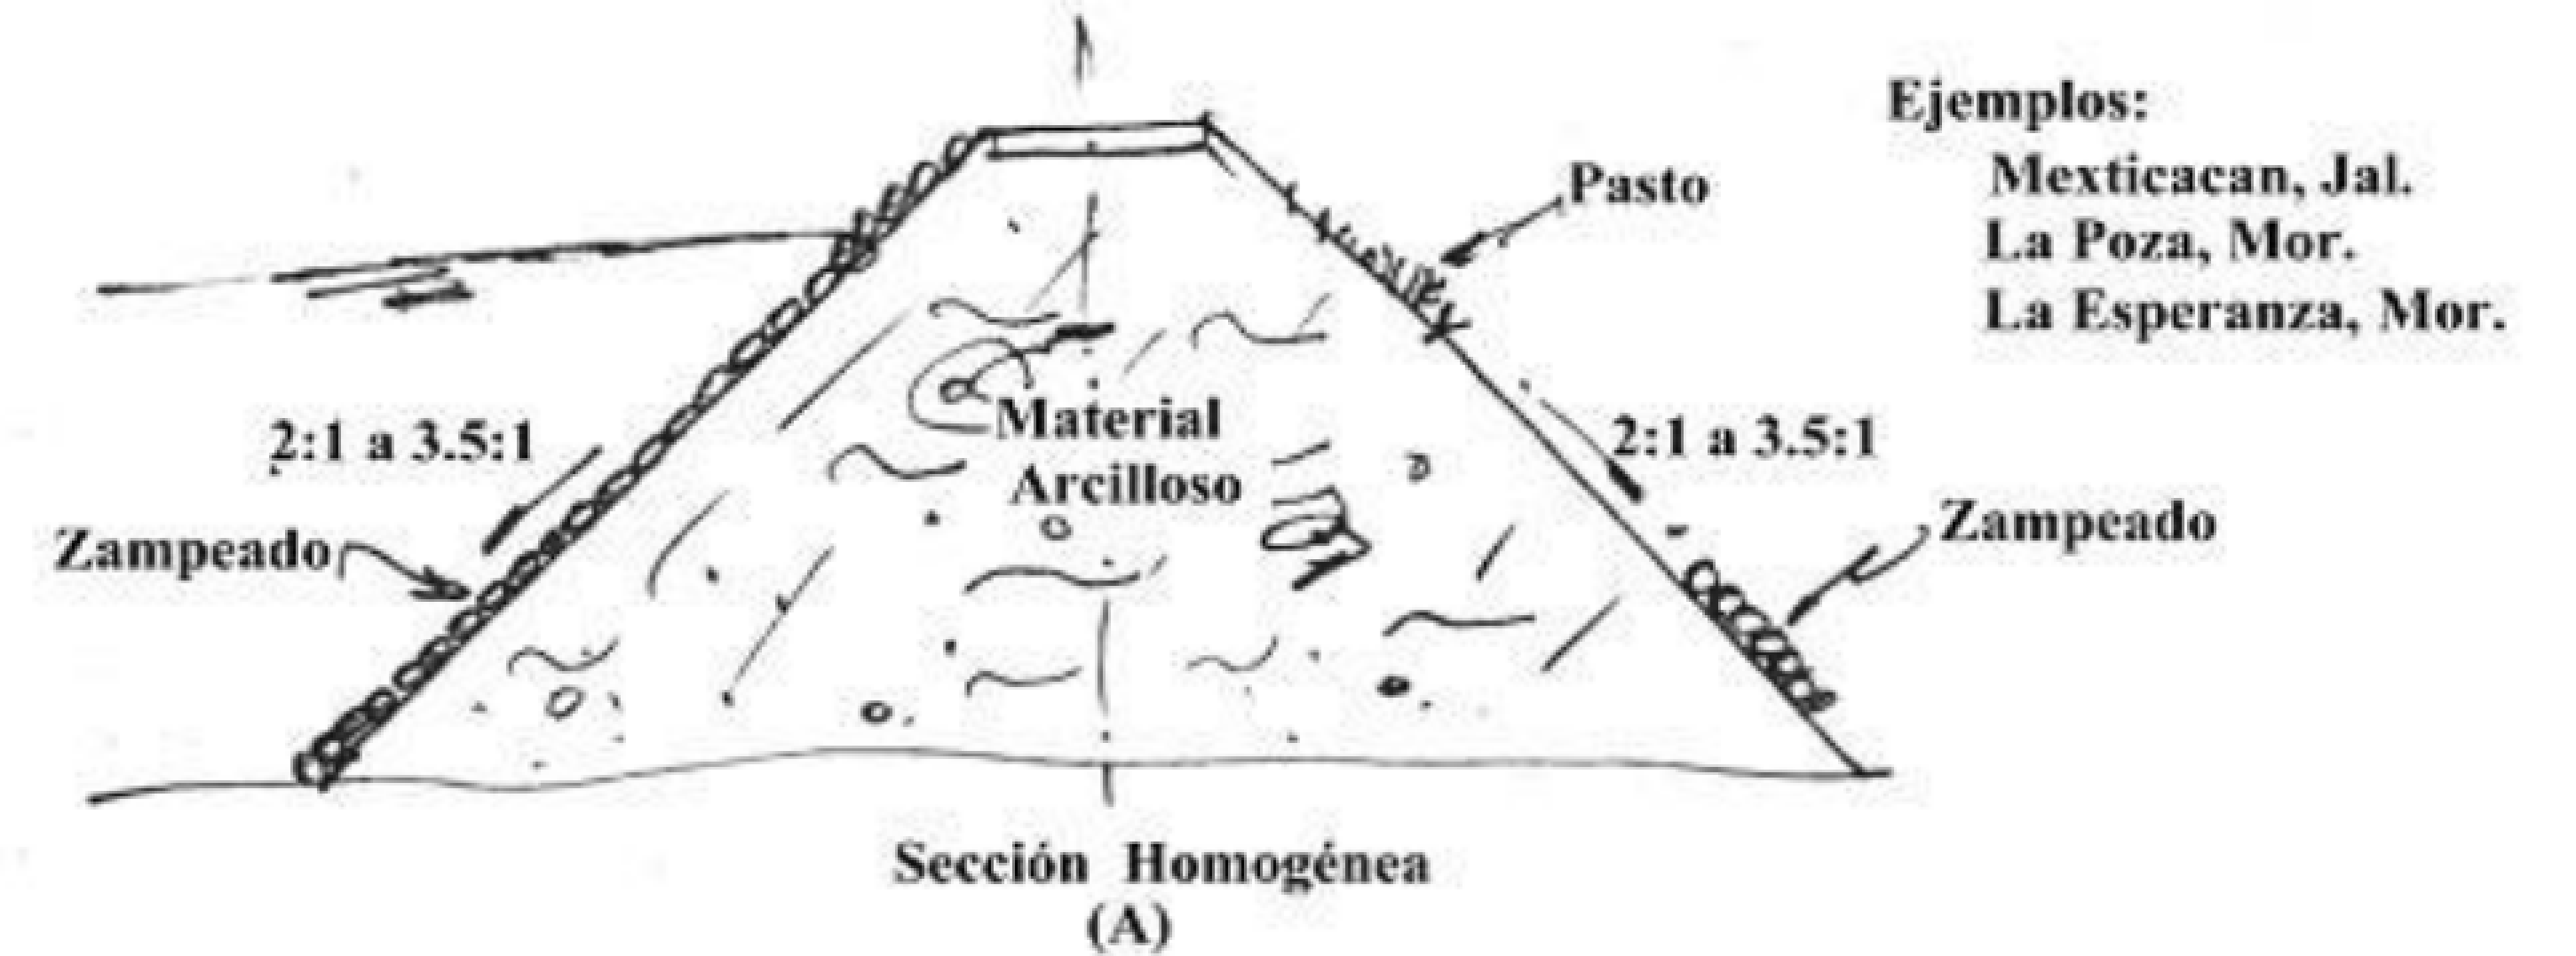
\includegraphics[width=0.5\textwidth]{fii37.png}}
		      \caption{Sección esquemática de presa de tierra tipo homogénea.}
		      \label{fii37}
	      \end{figure}
	\item Presa de tierra de sección tipo mixta.
	      \begin{figure}[h!]
		      \centerline{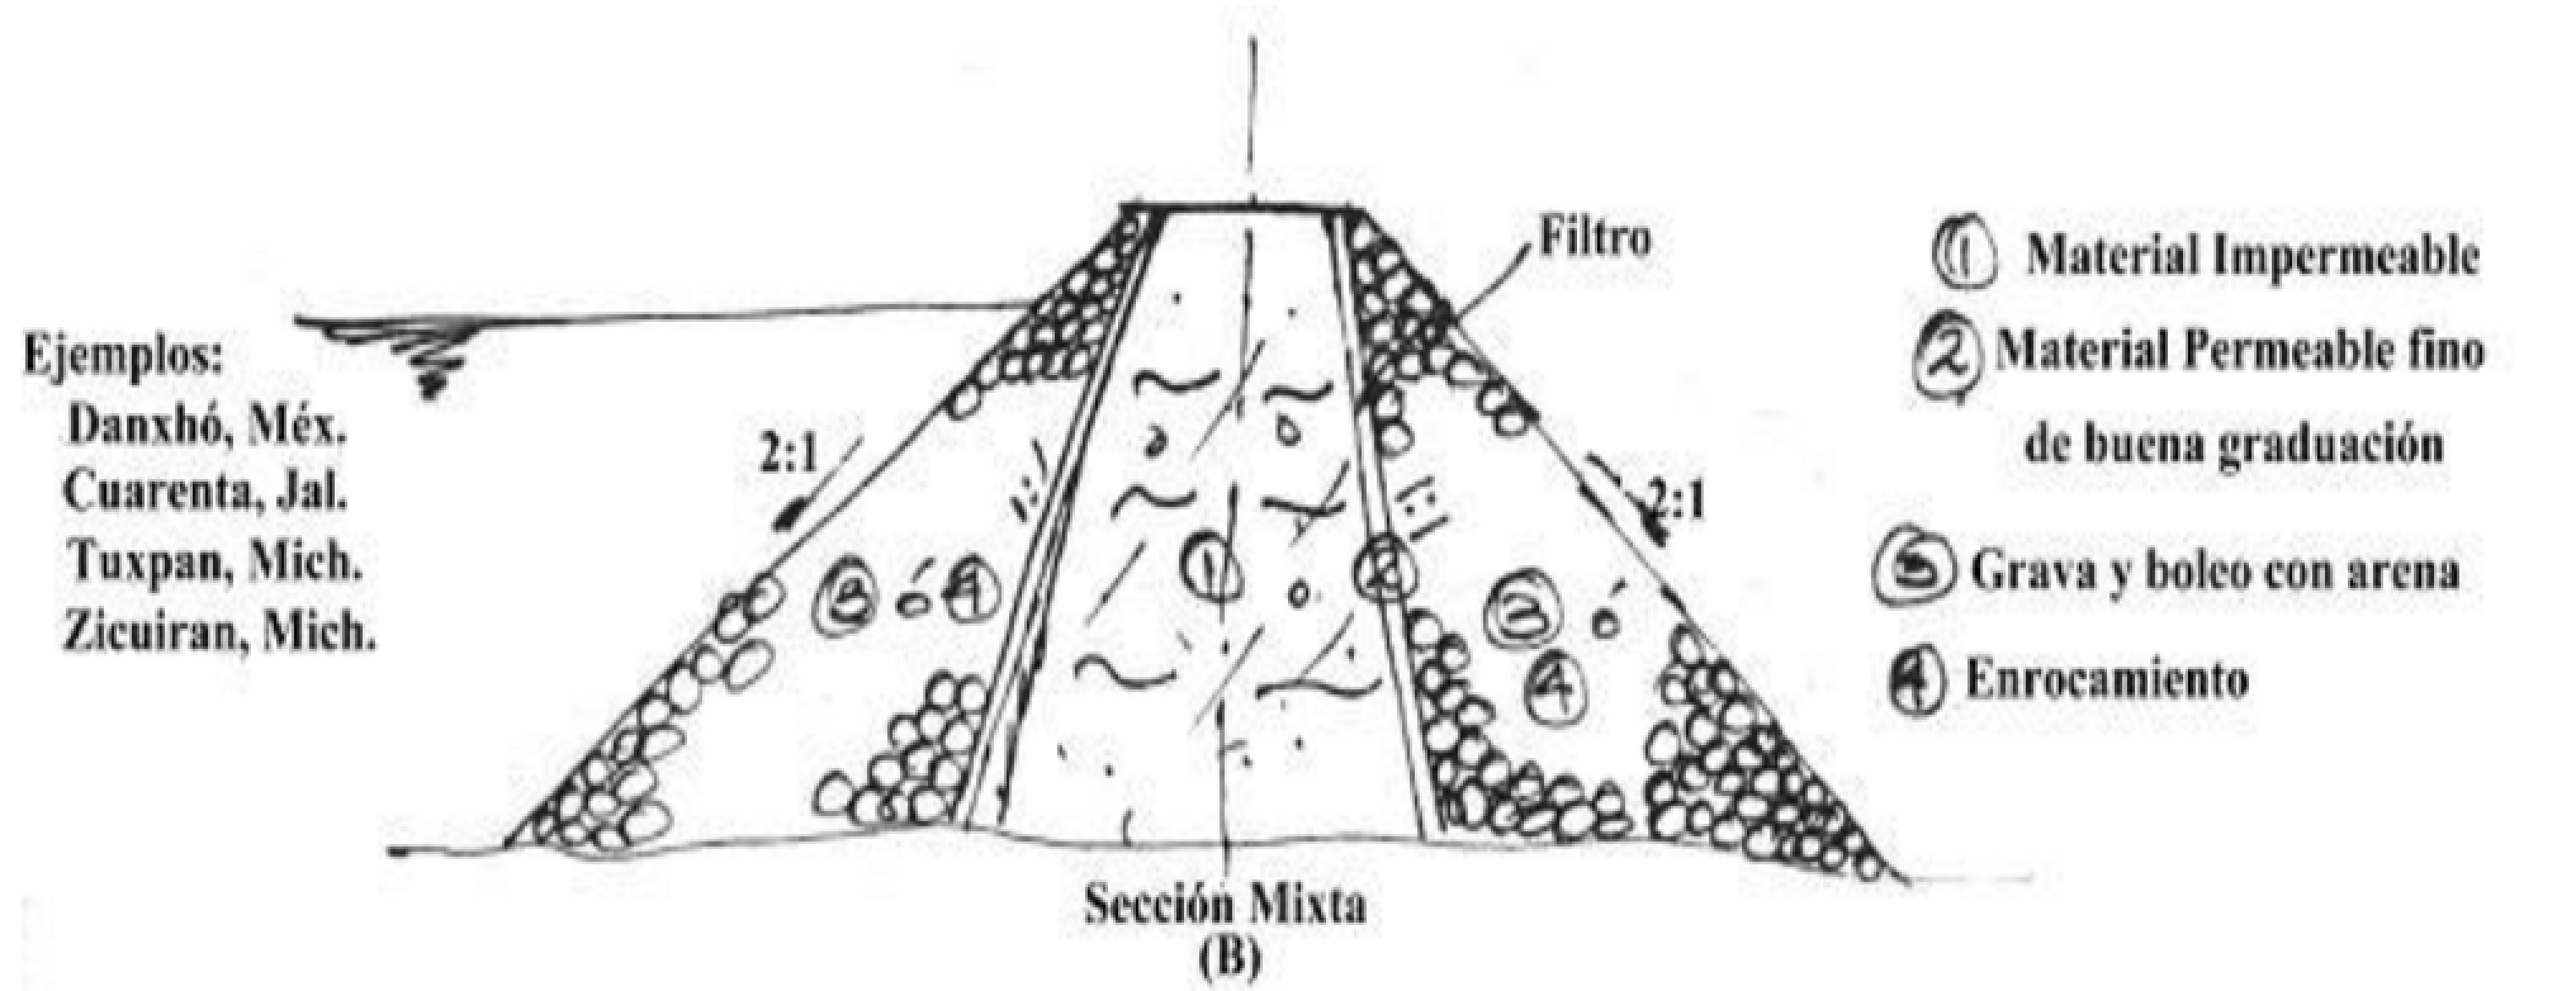
\includegraphics[width=0.5\textwidth]{fii38.png}}
		      \caption{Sección esquemática de presa de tierra tipo mixto.}
		      \label{fii38}
	      \end{figure}
	\item Presa de tierra de sección de materiales graduados
	      \begin{figure}[h!]
		      \centerline{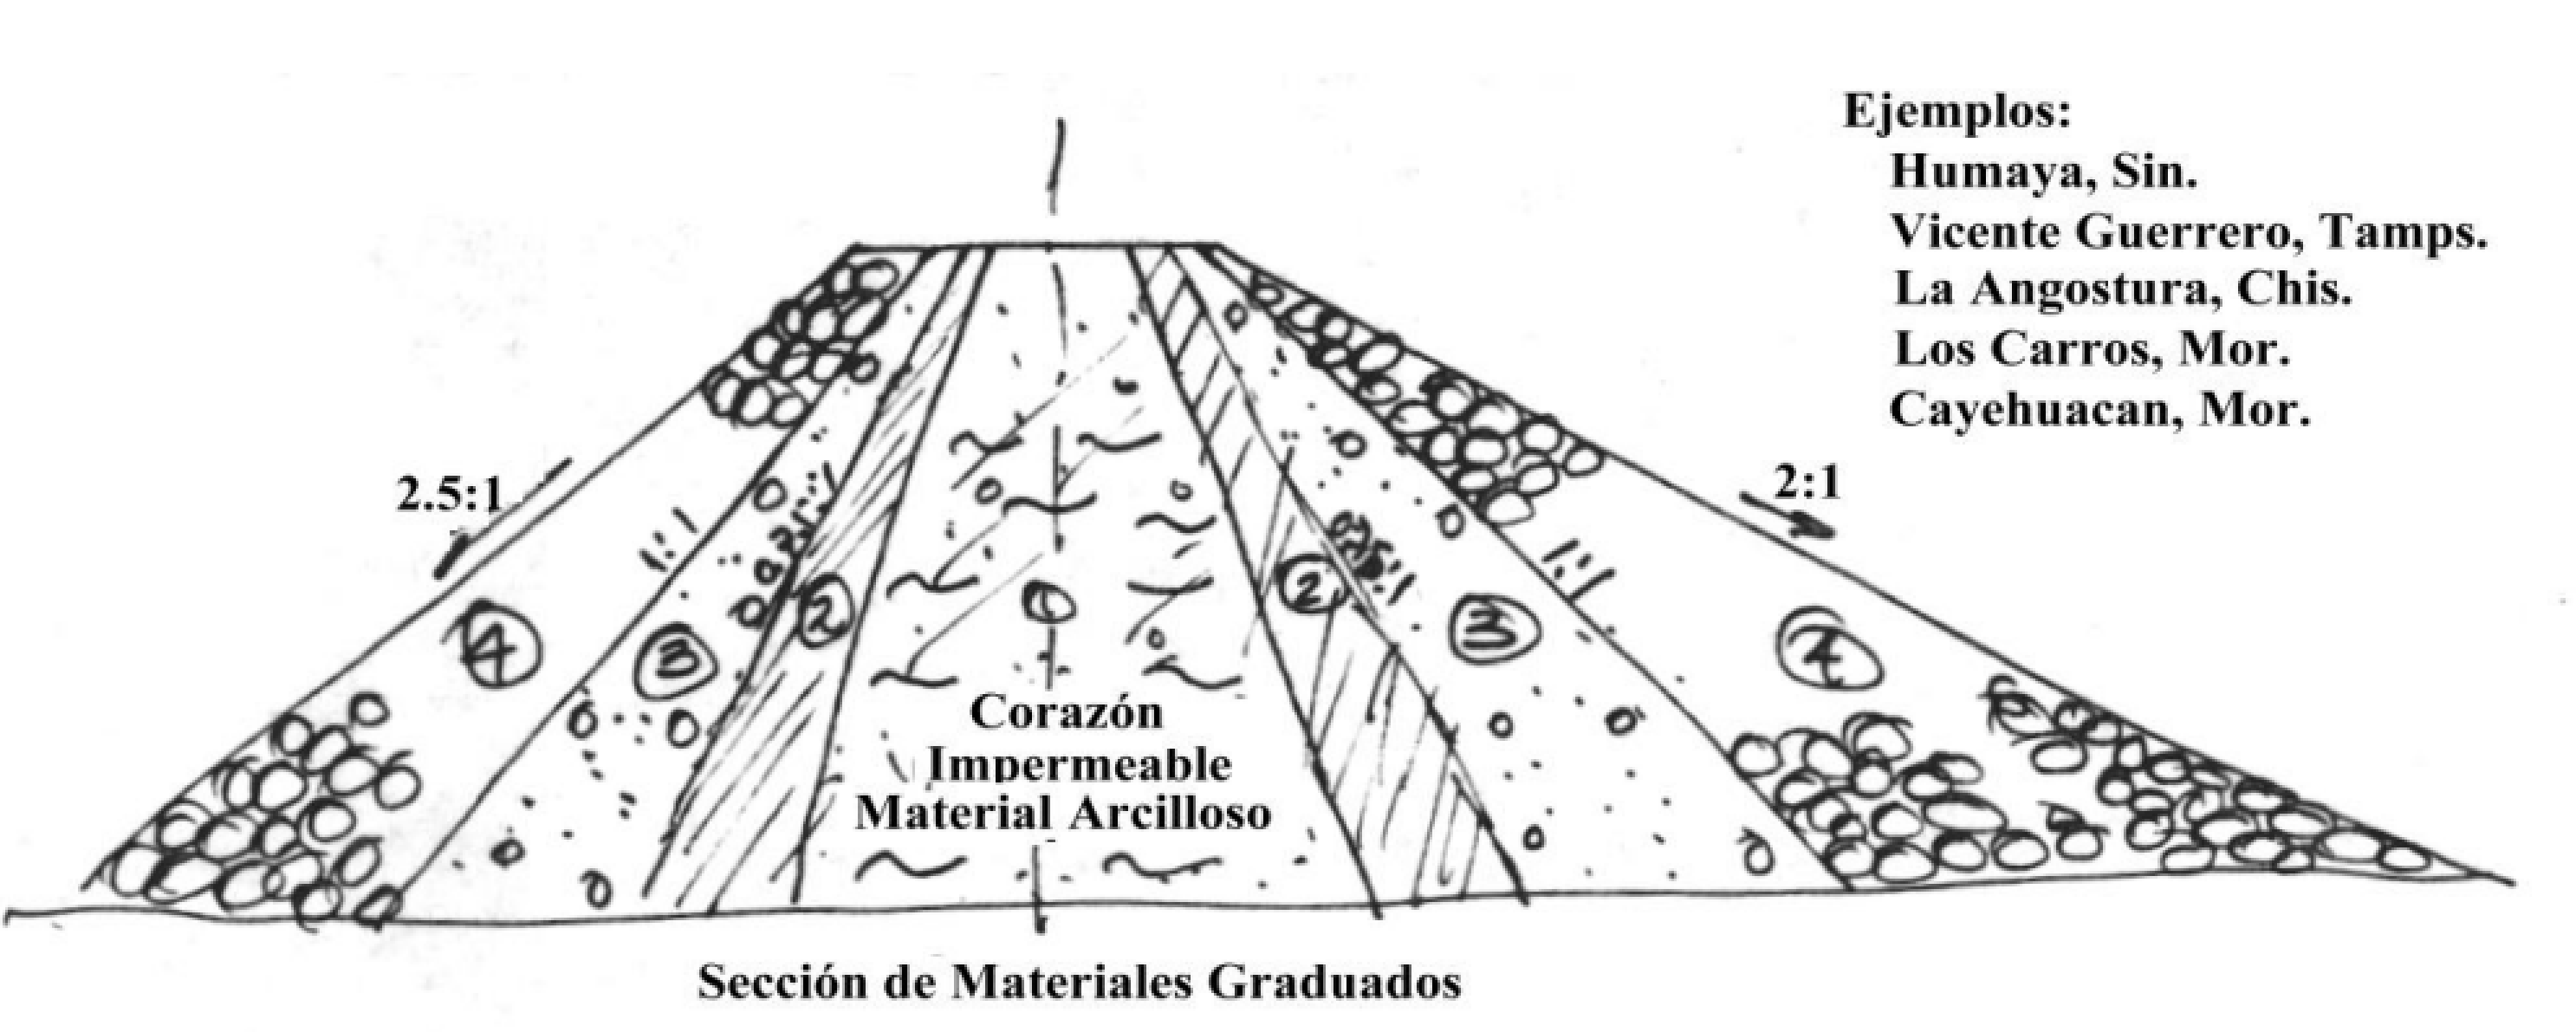
\includegraphics[width=0.5\textwidth]{fii39.png}}
		      \caption{Sección esquemática de presa de tierra tipo materiales graduados.}
		      \label{fii39}
	      \end{figure}
\end{enumerate}

\subsubsection{Presas de enrocamiento}

Estas presas ofrecen características intermedias entre las presas de gravedad y
las presas de tierra.

\begin{enumerate}[noitemsep]
	\item Paramento impermeable
	      \begin{figure}[h!]
		      \centerline{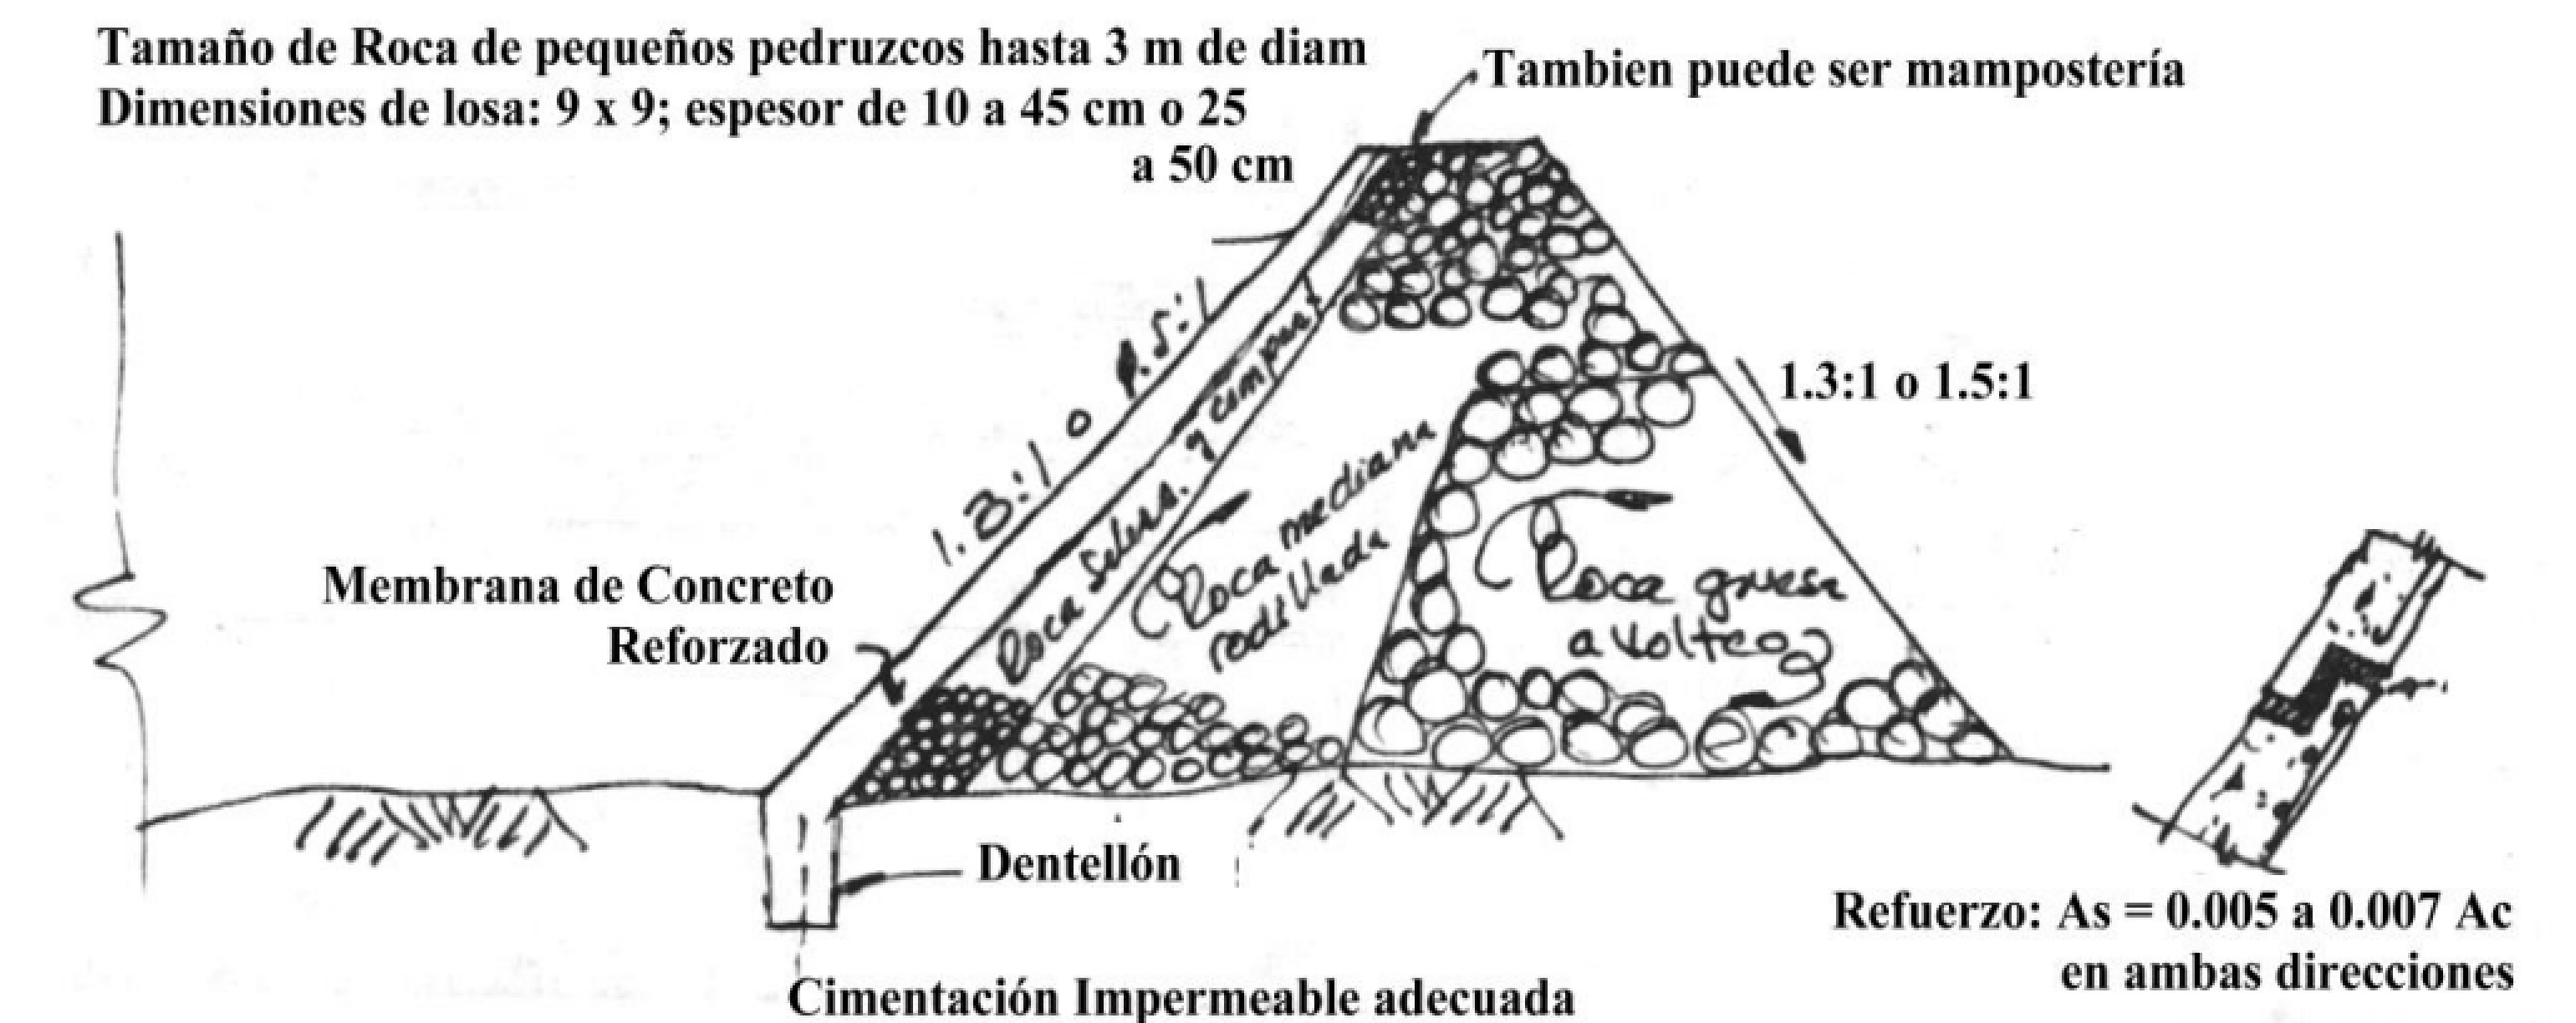
\includegraphics[width=0.5\textwidth]{fii40.png}}
		      \caption{ Sección esquemática de presa de enrocamiento.}
		      \label{fii40}
	      \end{figure}
	      \begin{figure}[h!]
		      \centerline{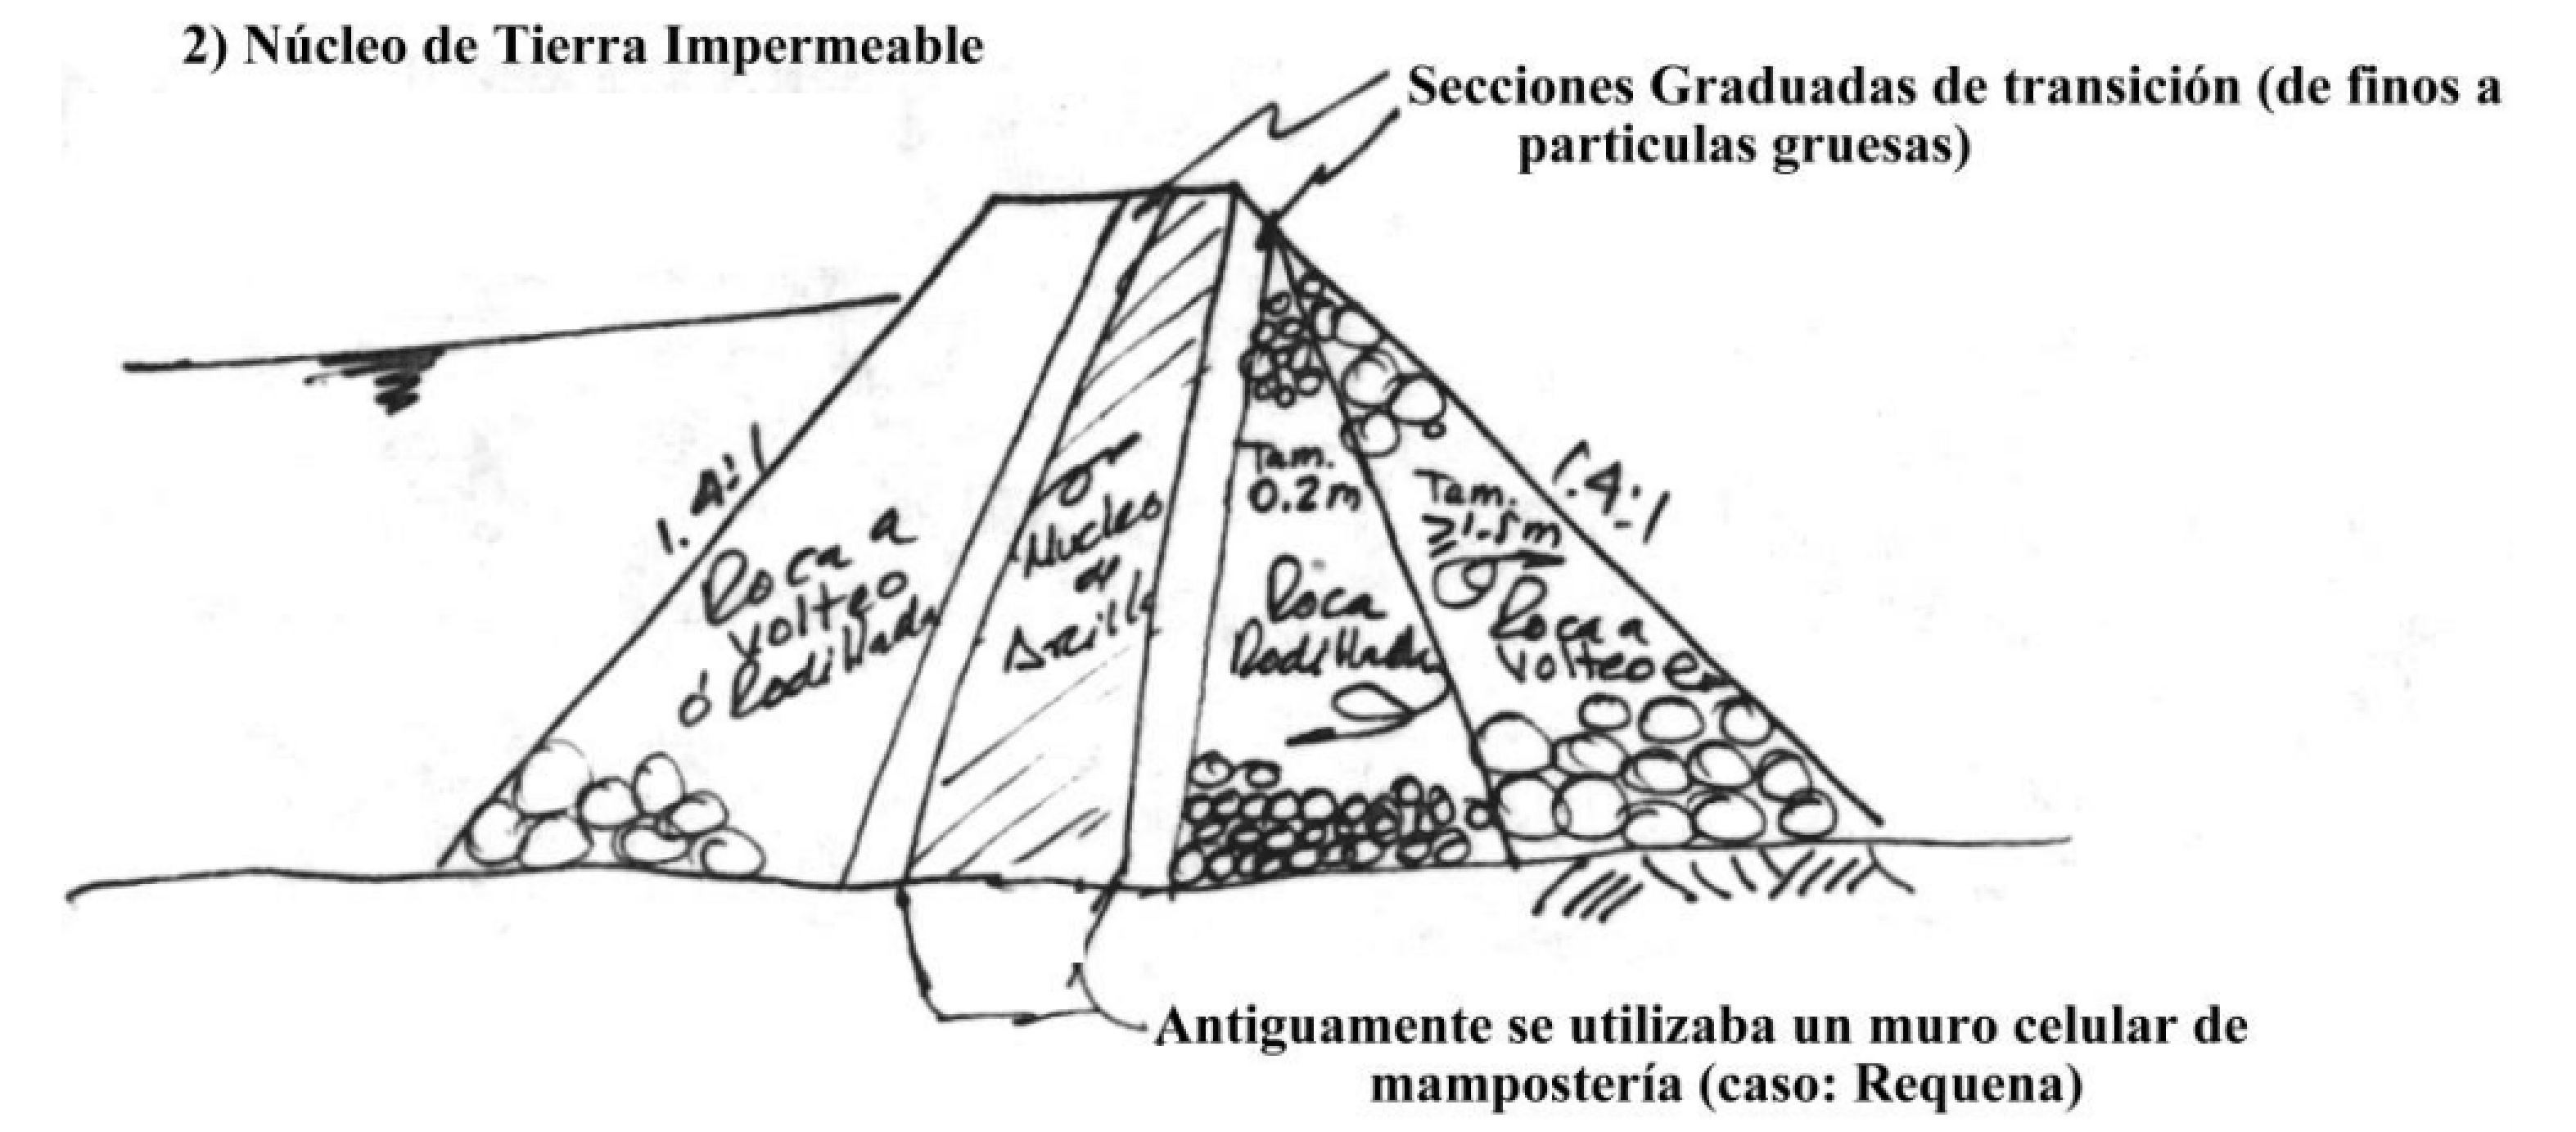
\includegraphics[width=0.5\textwidth]{fii41.png}}
		      \caption{Sección esquemática de presa de enrocamiento con corazón impermeable.}
		      \label{fii41}
	      \end{figure}
	\item Tipos misceláneos de presas: Presas compuestas
	      \begin{figure}[h!]
		      \centerline{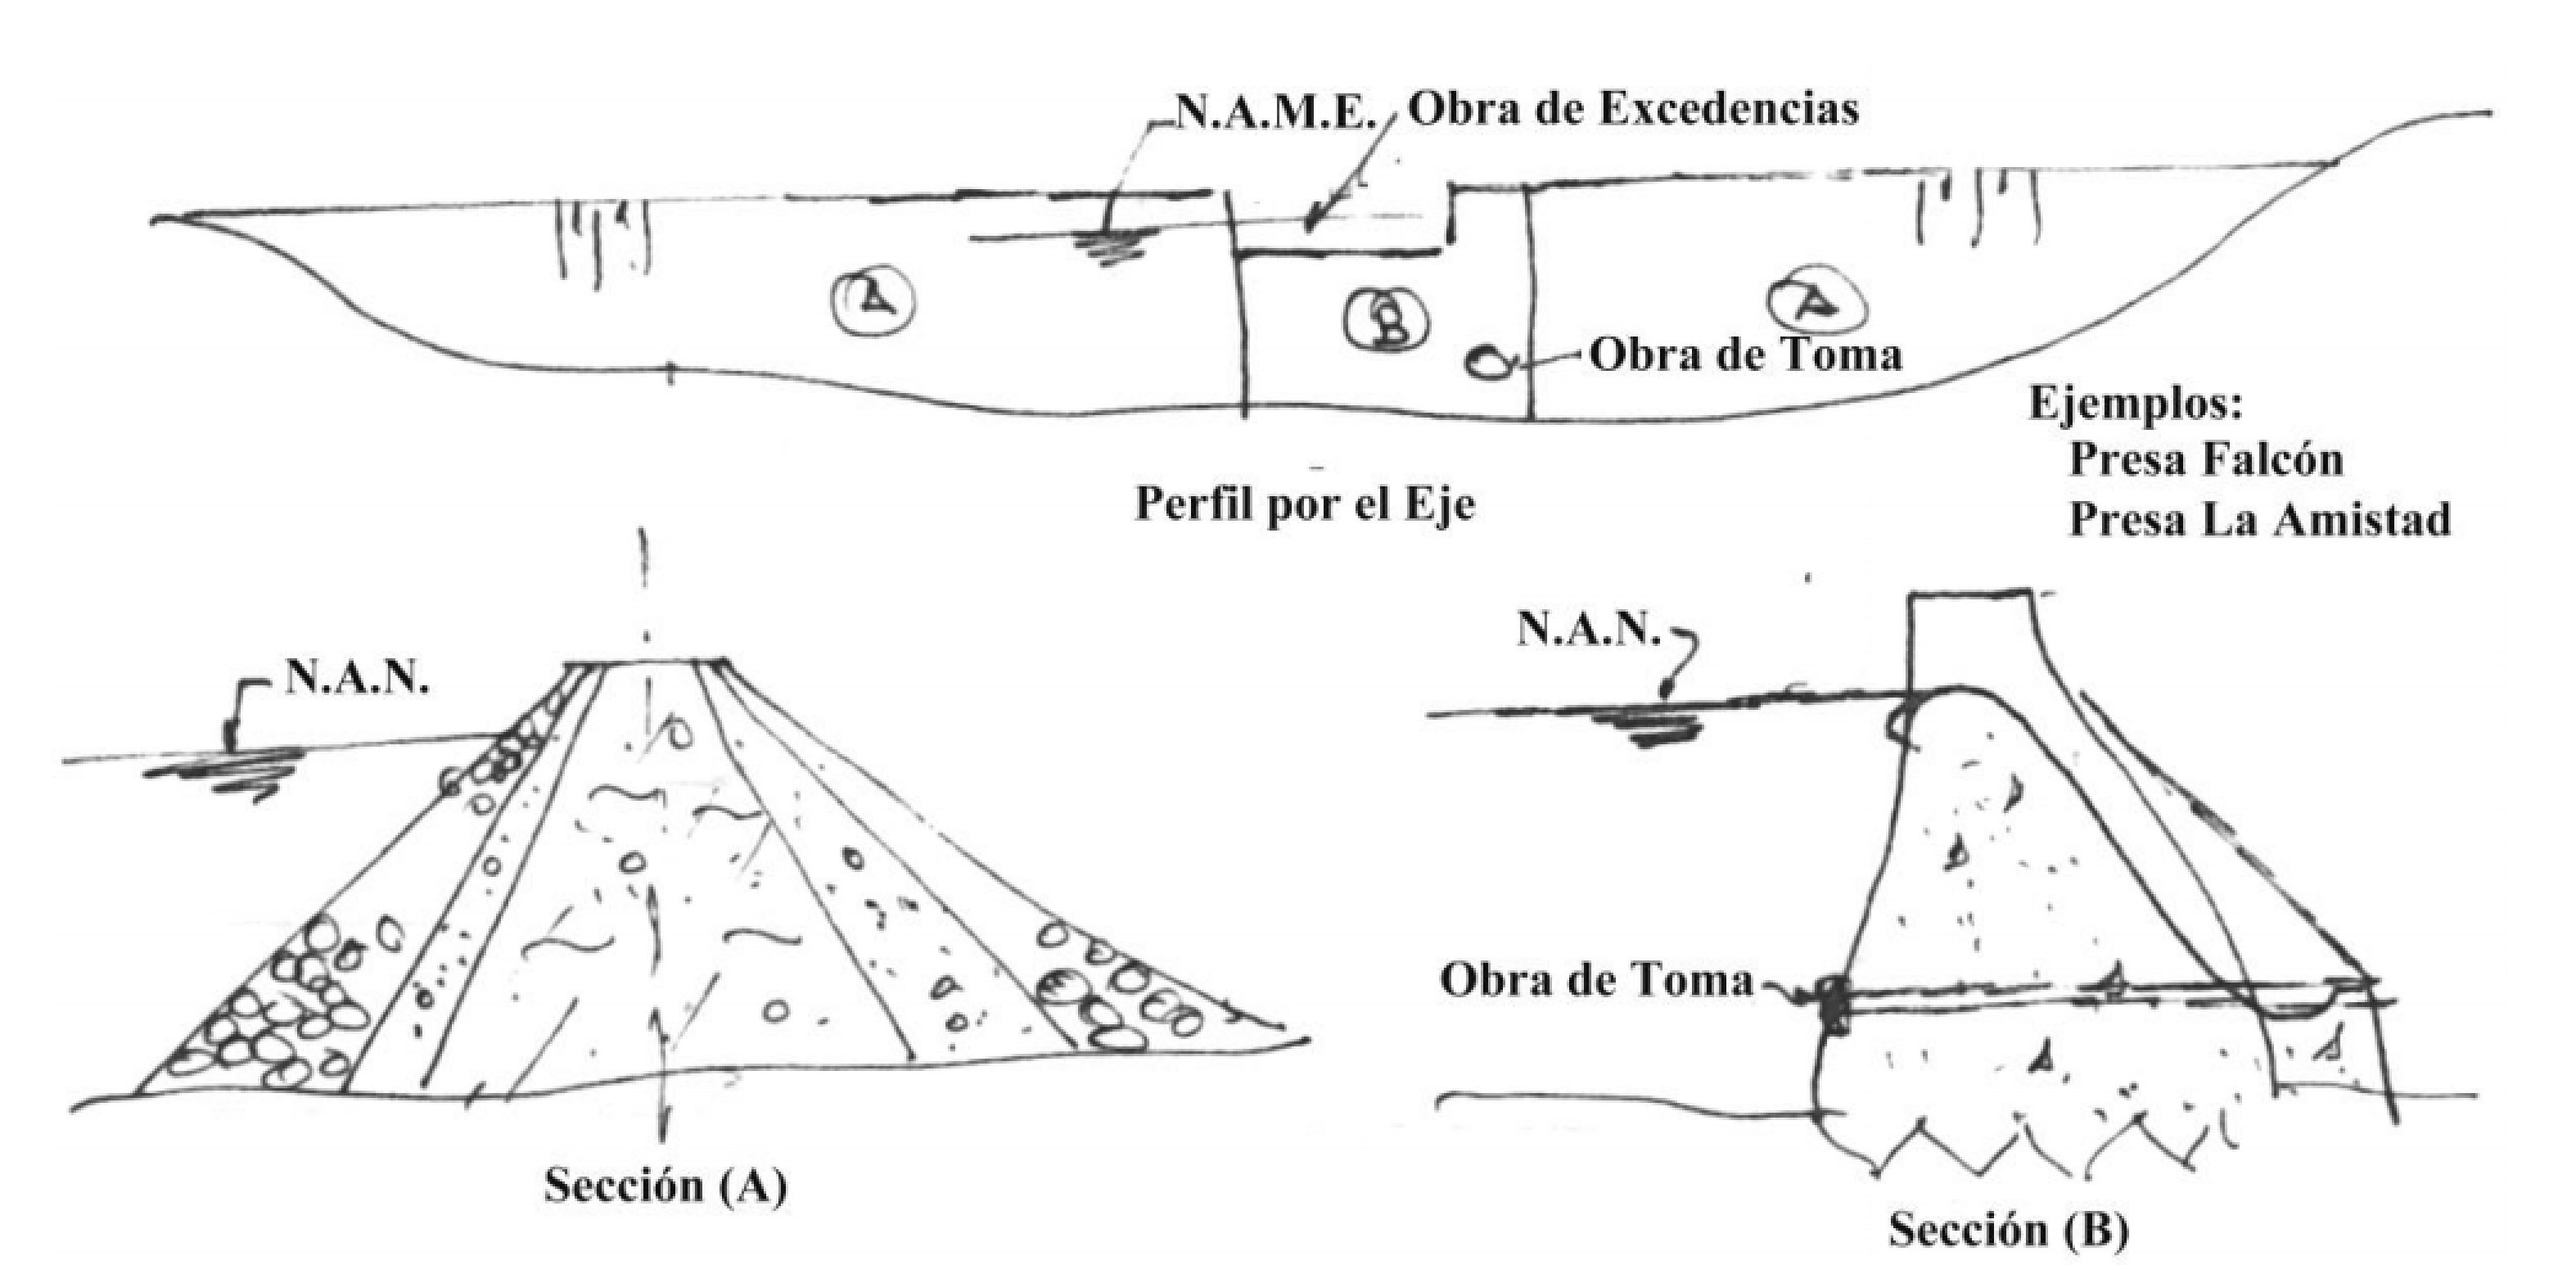
\includegraphics[width=0.5\textwidth]{fii42.png}}
		      \caption{Perfil por el eje y secciones esquemáticas de presa compuesta.}
		      \label{fii42}
	      \end{figure}
\end{enumerate}


\subsection{Obras de desvío}

\begin{definition}[Obras de desvío]
	La obra de desvío es el conjunto de estructuras que tiene por objeto separar o
	desviar el escurrimiento de un río de su cauce natural, durante la etapa de construcción
	de una obra de retención, para poder así trabajar en seco en el sitio de la cortina y
	obras auxiliares. El agua subálvea es aquella que está debajo del álveo de un río o arroyo.
\end{definition}



\subsubsection{Tipo de estructuras integrantes de una obra de desvío.}

Las estructuras integrantes de una obra de desvío pueden ser:
\begin{enumerate}[noitemsep]
	\item  Canal o Tajo temporal
	      \begin{figure}[h!]
		      \centerline{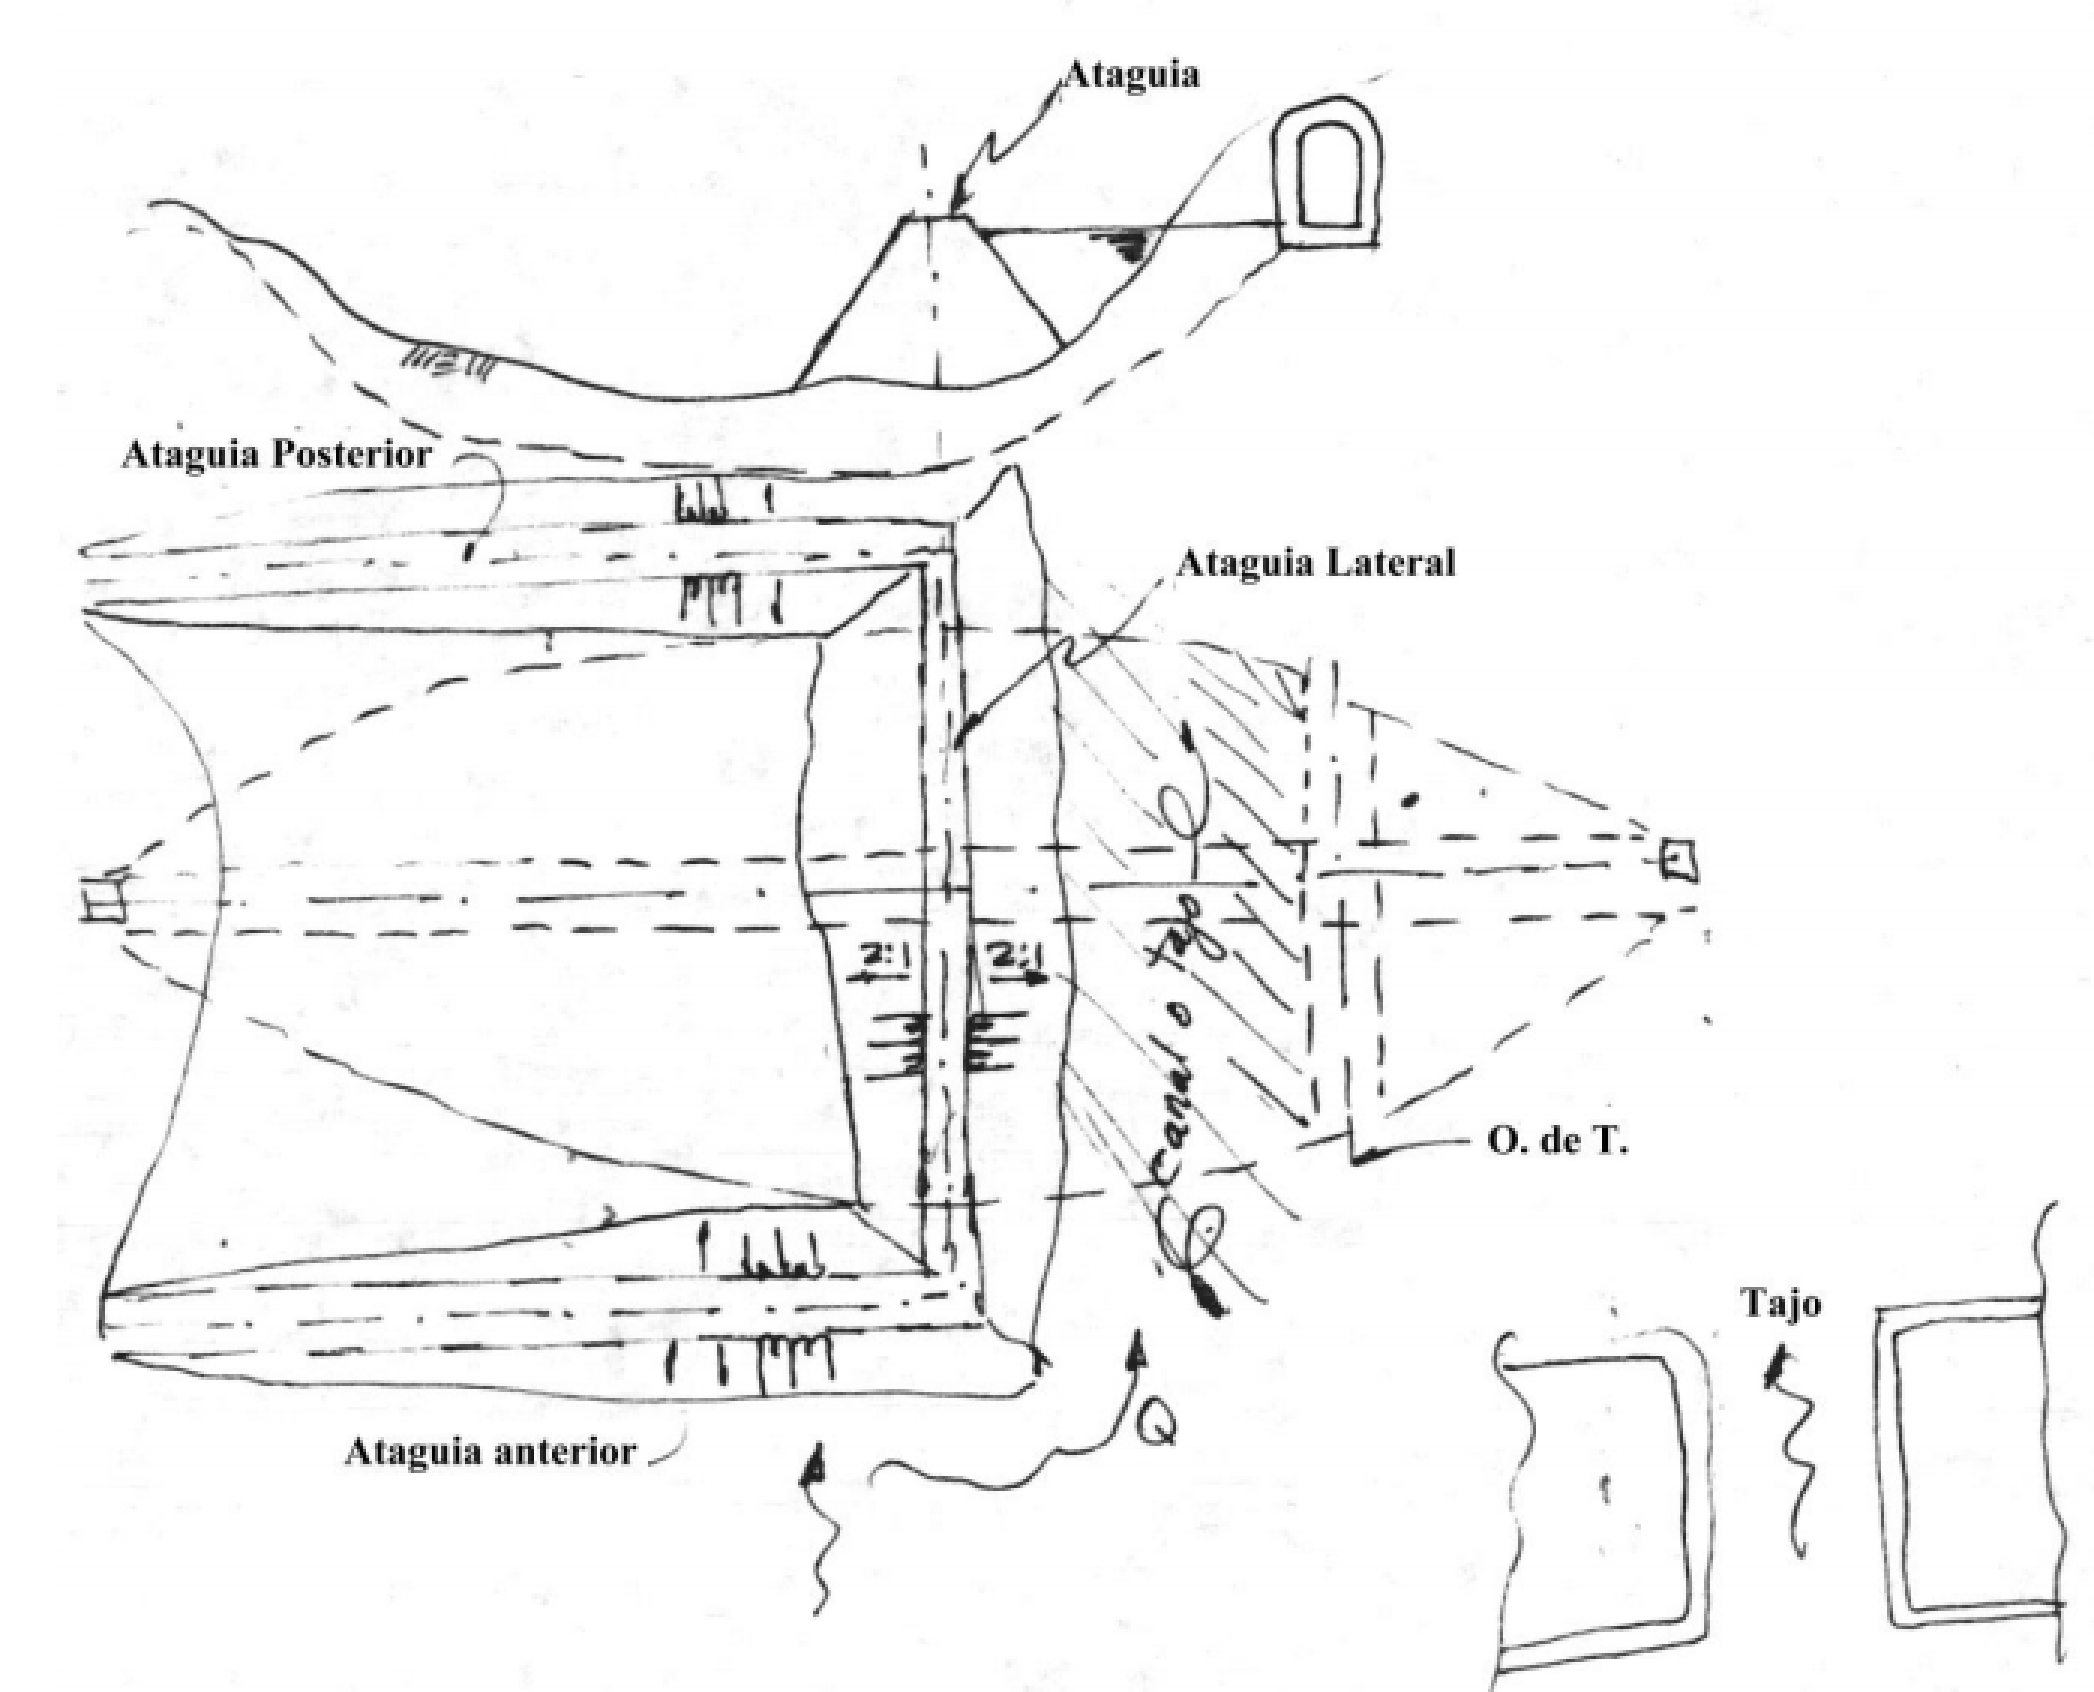
\includegraphics[width=0.5\textwidth]{fii43.png}}
		      \caption{Obra de desvío conformada con un canal o tajo temporal.}
		      \label{fii43}
	      \end{figure}
	\item  Hueco o paso temporal a través de la cortina de concreto
	\item  Conducto a través del cuerpo de una cortina de materiales graduados
	\item  Túneles a través de las laderas de las boquillas
\end{enumerate}

La Ataguía es un dique o barrera temporal que se emplea para desviar la
corriente o para encerrar un área determinada, permitiendo la construcción dentro de
ella, aún por debajo del nivel del escurrimiento.

\begin{enumerate}
	\item Tierra
	\item Tabla estacados:Madera o acero hincados en el terreno y apoyados por una serie de
	      marcos de madera o fierro para resistir el empuje. Ó Enhuacalados de madera, relleno de roca con tierra
	      \begin{figure}[h!]
		      \centerline{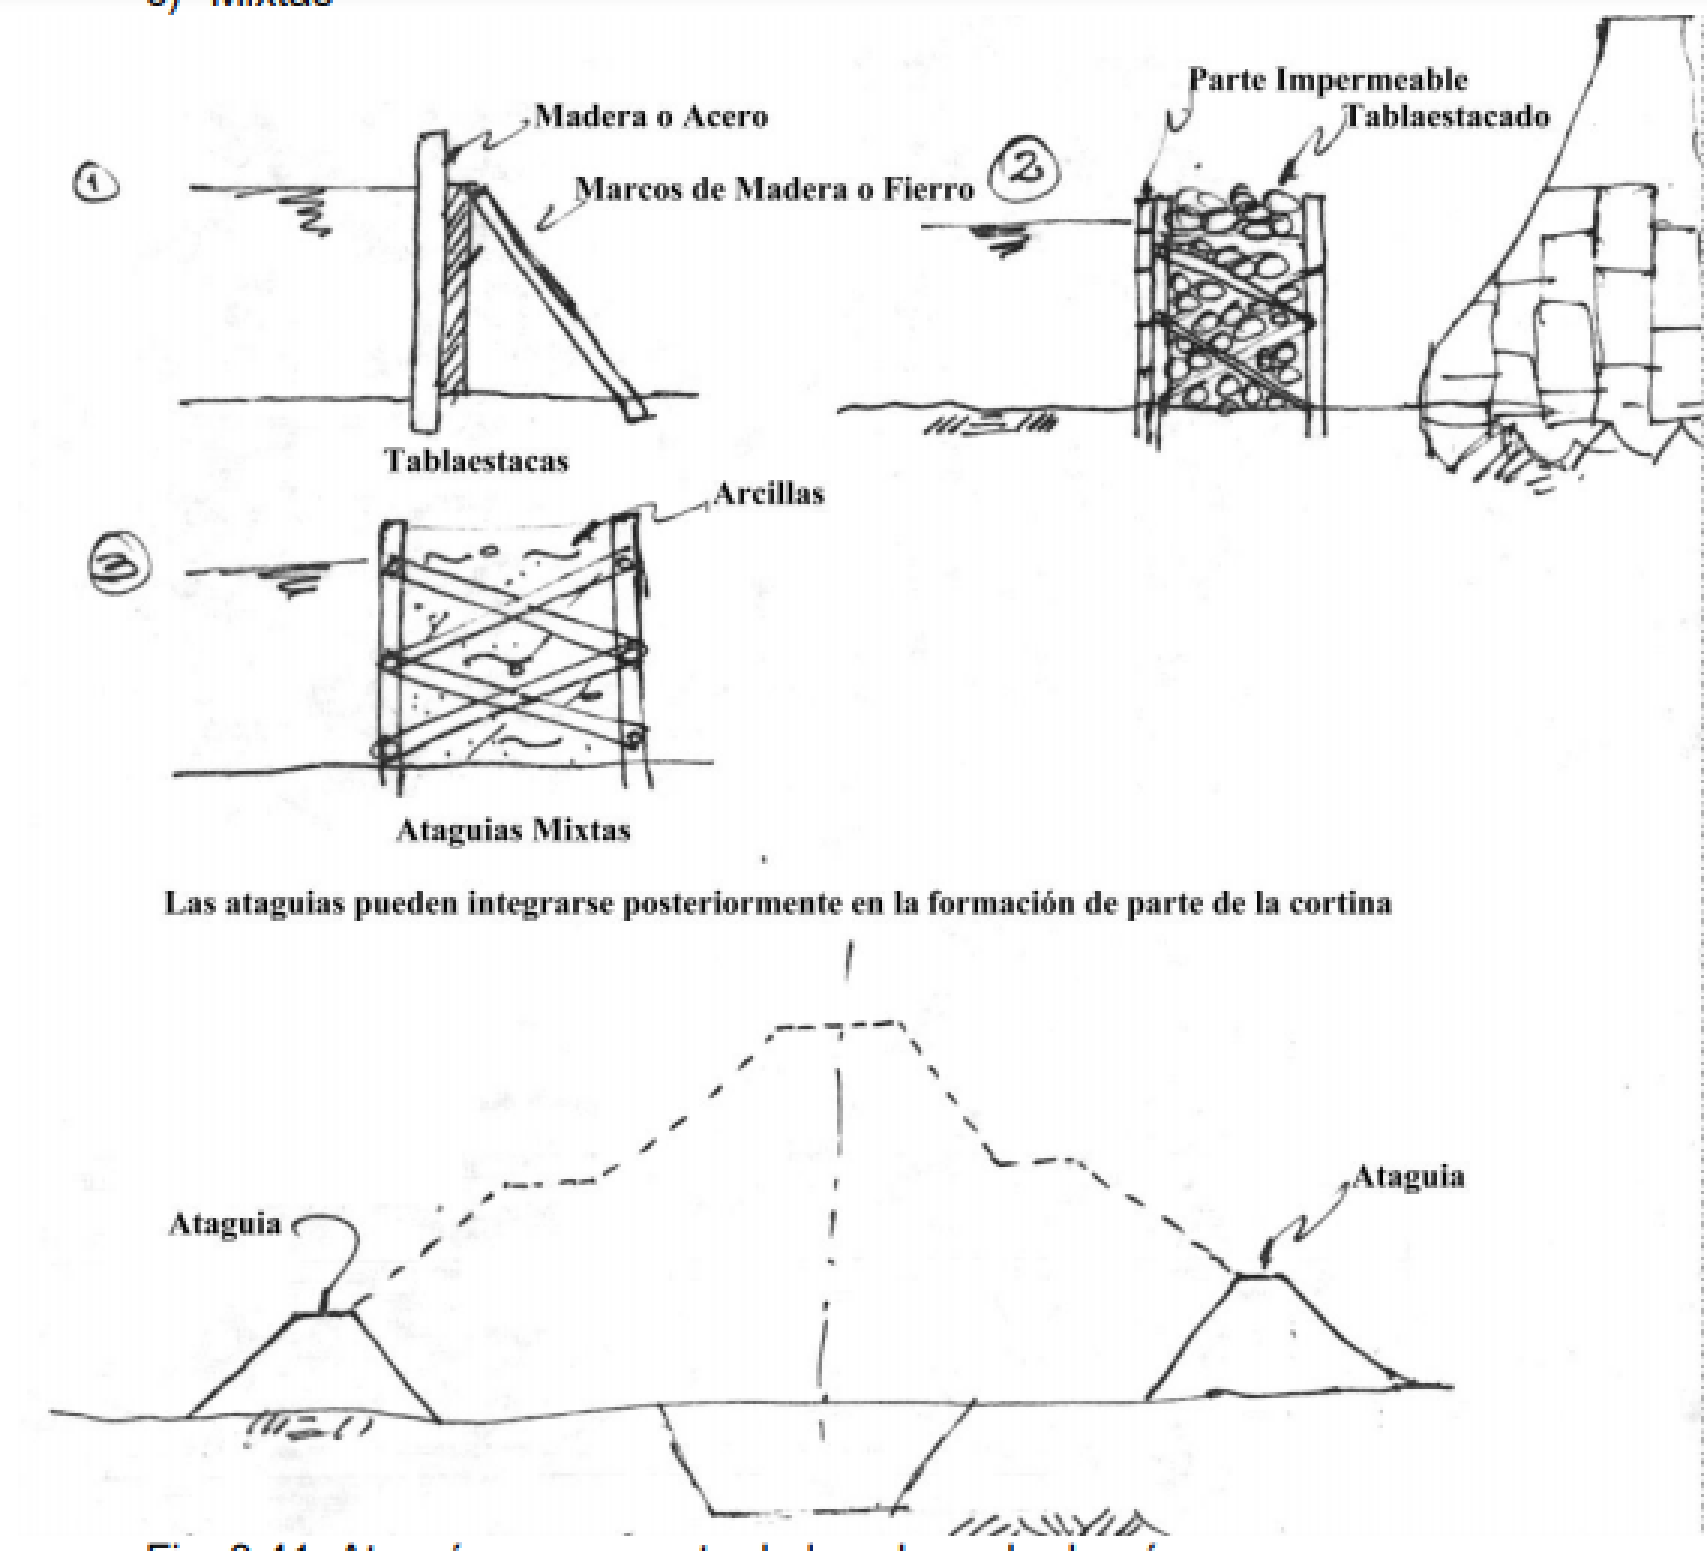
\includegraphics[width=0.5\textwidth]{fii44.png}}
		      \caption{Ataguías como parte de las obras de desvío.}
		      \label{fii44}
	      \end{figure}
	\item Mixtas
\end{enumerate}

Las principales consideraciones para la planeación de las ataguías son:

\begin{enumerate}
	\item Suficiente altura
	\item Seguridad durante el periodo de desvío
	\item Previsión para removerlas cuando ya no se empleen.
\end{enumerate}

\textbf{Hueco o paso temporal} a través de la cortina de concreto
Características: Son muy caros, pero más efectivos, mantienen seco el lugar de construcción, trabajan a superficie libre
Pueden ir revestidos, reforzados con acero y concreto, o ademado con  acero. Forman parte de la obra de toma u obra de excedencias (infiernillo). Son para obras de gran importancia.

\begin{figure}[h!]
	\centerline{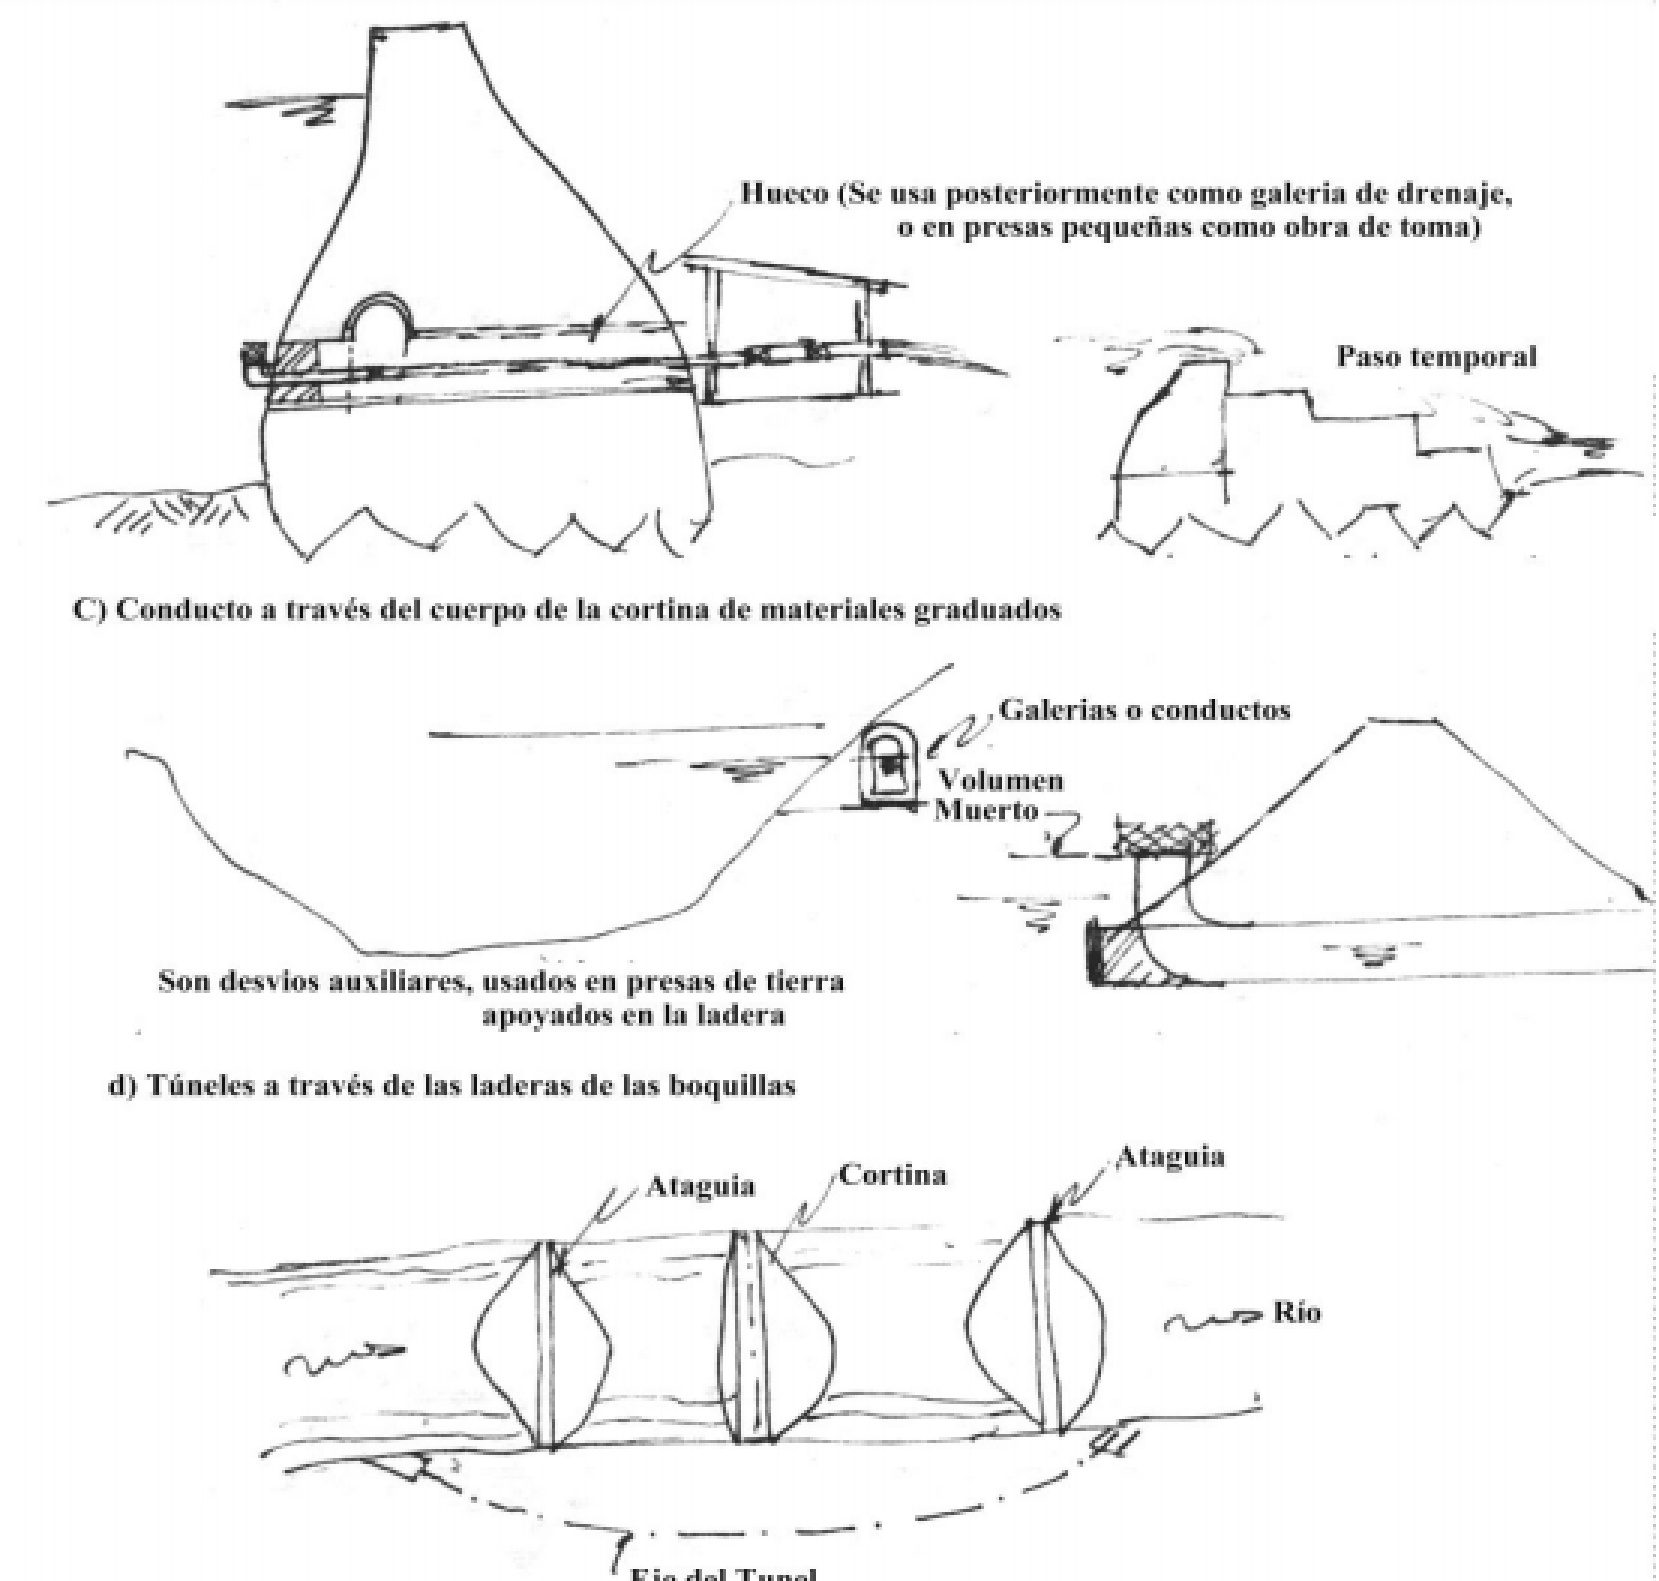
\includegraphics[width=0.5\textwidth]{fii45.png}}
	\caption{Obras de desvío bajo diferentes alternativas.}
	\label{fii45}
\end{figure}



\subsubsection{Obras de Toma:} La función de esta obra es manejar las extracciones para
satisfacer la demanda que los diferentes beneficios exigen.


\subsubsection{Obras de excedencias:} La función es dar salida a las aguas de escurrimiento que
no pueden ser almacenadas por haber llegado a un cierto nivel que muestra la
capacidad total.



\subsection{Obras de toma}

\begin{definition}[Obras de toma]
	La obra de toma es el conjunto de estructuras y equipos requeridos para la
	operación segura y controlada del agua embalsada, extraída con el objeto de satisfacer
	las necesidades de las demandas, para el cual fue proyectado el almacenamiento.
\end{definition}

\subsubsection{Partes esenciales}

\begin{itemize}
	\item Conductos (canal, tubería, túnel y/o galería)
	\item Sistemas de obturación (estructura mecánica con elementos de cierre).
\end{itemize}

Ordenamiento de las partes en el sentido de la corriente:

\begin{enumerate}
	\item Canal de acceso
	\item Estructura de rejillas
	\item Conducto
	\item Equipo y sistema de obturación
	\item Elementos de protección y control
	\item Estructuras terminales
\end{enumerate}

\subsubsection{Clasificación de las obras de toma}

\begin{enumerate}[noitemsep]
	\item Según el propósito
	      \begin{enumerate}
		      \item Para generar energía
		      \item Para riego
		      \item Para finalidades múltiples
	      \end{enumerate}
	\item Según la ubicación del sistema de operación
	      \begin{enumerate}
		      \item Que se opera en la entrada de la obra de toma o del conducto
		      \item Que se opera en la parte media del conducto
		      \item Que se opera al final del conducto
	      \end{enumerate}
	\item Según la estructura donde se ubica el mecanismo de obturación
	      \begin{enumerate}
		      \item Tipo Torre
		      \item Tipo lumbrera
		      \item Tipo tubería a presión y válvulas
	      \end{enumerate}
	\item Según el tipo de construcción del conducto
	      \begin{enumerate}
		      \item Conducto excavado y colado a cielo abierto
		      \item Túneles perforados en las laderas
		      \item Conducto ahogado en el cuerpo de la cortina
	      \end{enumerate}
	\item Según la posición de la Obra de Toma
	      \begin{enumerate}
		      \item En una de las márgenes
		      \item En ambas márgenes
		      \item En un solo nivel
		      \item En varios niveles (Toma alta, toma baja)
	      \end{enumerate}
	\item Según la característica de la descarga.
	      \begin{enumerate}
		      \item Se descarga a un canal de conducción
		      \item Se descarga directamente al río
		      \item Descarga a un sistema de tubería forzada (a presión)
	      \end{enumerate}
\end{enumerate}

\subsubsection{Localización de la Obra de Toma}

\begin{enumerate}
	\item Respecto a la cortina.
	      \begin{enumerate}
		      \item En el cuerpo de la cortina (sólo de materiales rígidos: gravedad (de concreto
		            o mampostería, arco, arco-gravedad, etc$\dots$)
		      \item Fuera del cuerpo de la cortina (utilizada en cortinas de materiales flexibles,
		            ubicada en una de las laderas en excavación o en perforación de túnel).
	      \end{enumerate}
	\item Respecto a niveles de almacenamiento
\end{enumerate}

El nivel de la obra de toma, lo fija el N.A.mín. (Nivel de Aguas mínimo) dado por
la capacidad muerta en el almacenamiento, integrado por el volumen de azolves, cría
de peces, recreación y otros.

\subsubsection{Tipos más frecuentes de Obra de Toma}

\begin{enumerate}[noitemsep]
	\item Canal en tomas Altas
	\item Torre y galería (funcionando como canal)
	      \begin{figure}[h!]
		      \centerline{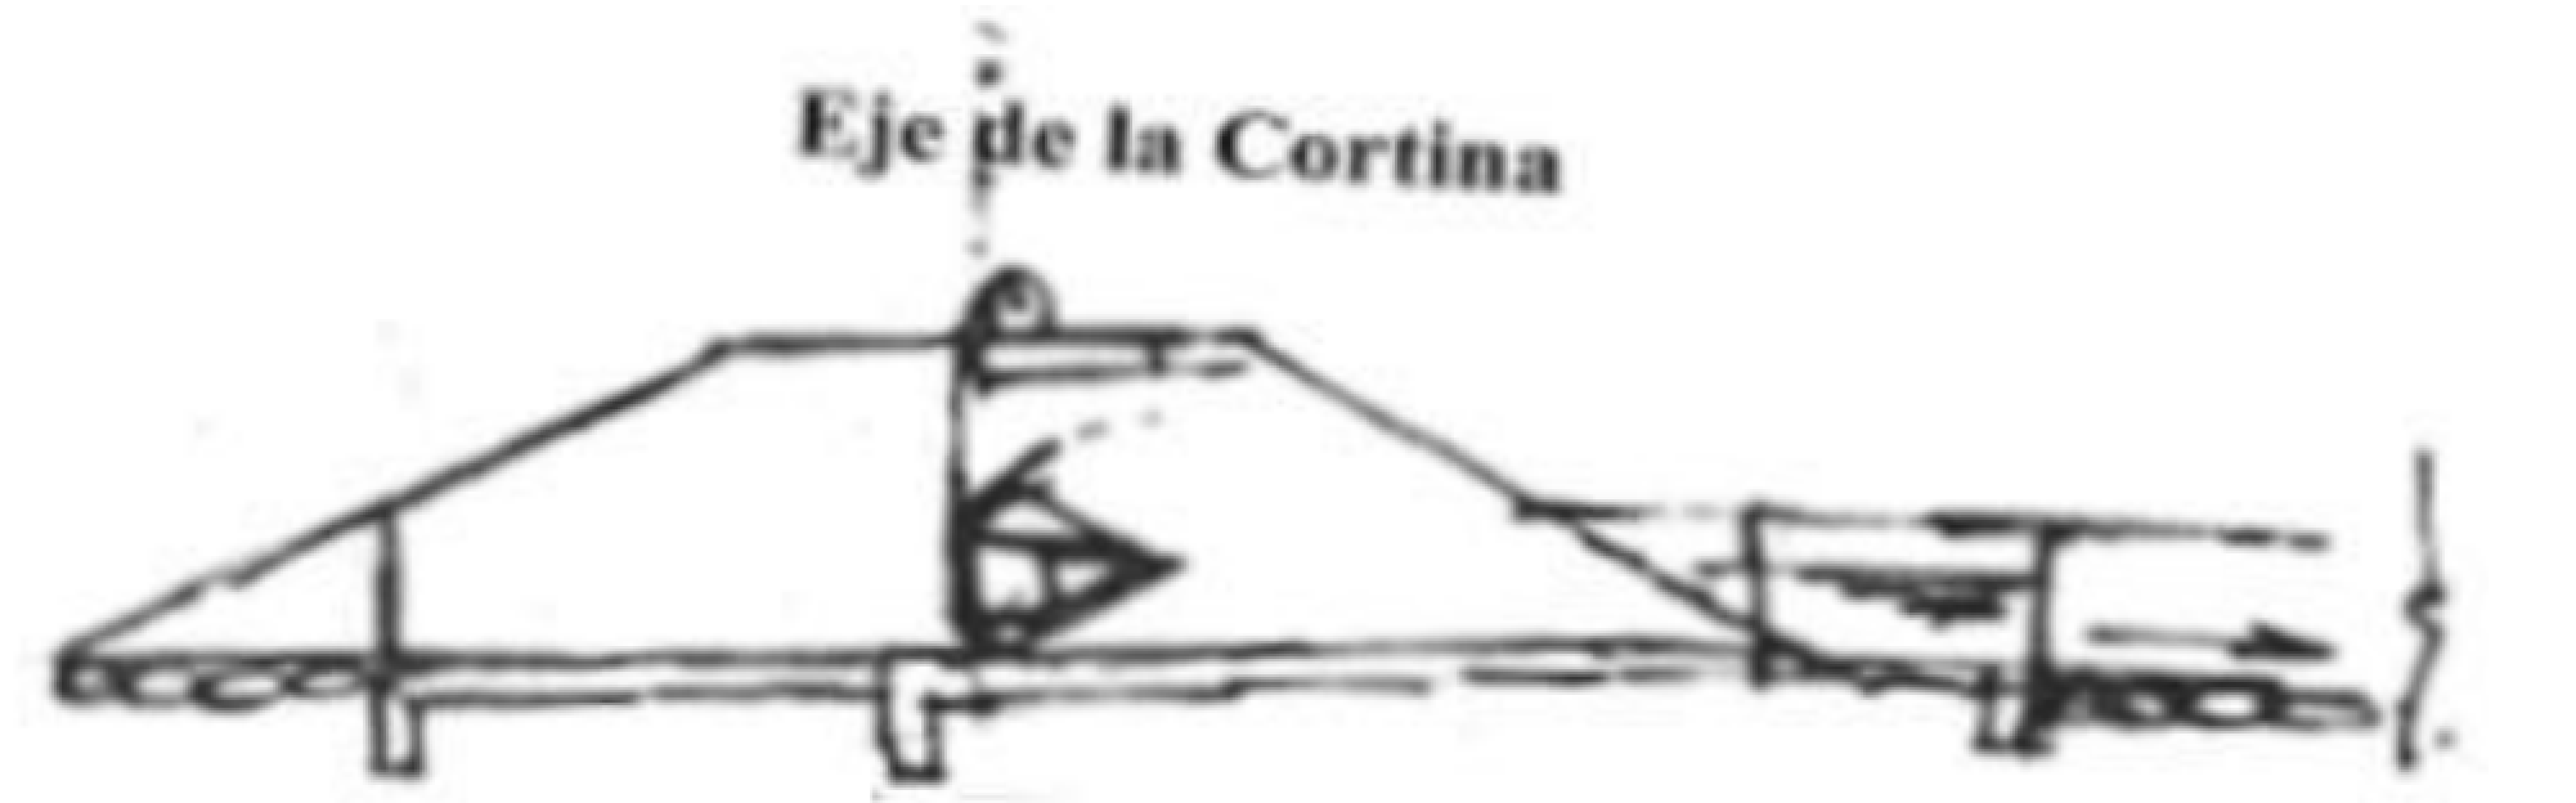
\includegraphics[width=0.5\textwidth]{fii46.png}}
		      \caption{Perfil esquemático de obra de toma tipo torre y galería.}
		      \label{fii46}
	      \end{figure}
	\item Tubería a presión
	      \begin{figure}[h!]
		      \centerline{\includegraphics[width=0.5\textwidth]{fii47.png}}
		      \caption{Perfil esquemático de obra de toma tipo tubería a presión y válvulas a
			      la salida.}
	      \end{figure}
	      \label{fii47}
	\item Galería con tubería a presión
	      \begin{figure}[h!]
		      \centerline{\includegraphics[width=0.5\textwidth]{fii48.png}}
		      \caption{Perfil esquemático de obra de toma tipo tubería a presión y válvulas a
			      la salida.}
		      \label{fii48}
	      \end{figure}
	\item Tipos mixtos.
\end{enumerate}

\subsection{Obras de excedencias}

\begin{definition}[Obras de excedencias]
	La obra de excedencias o vertedor de demasías es la estructura que tiene por
	objeto dar salida a las aguas excedentes del almacenamiento, protegiendo la cortina,
	obra de toma y demás estructuras al impedir que el agua, que ya no puede ser
	almacenada (por rebasar el N.A.N.), desborde sobre la obra de retención y la destruya.
\end{definition}

\subsubsection{Partes de que consta}

\begin{itemize}
	\item Canal de acceso
	\item Cresta vertedora
	\item Canal colector
	\item Sección de control
	\item Canal de descarga
	\item Estructura disipadora o disipador de energía
	\item Canal de salida al cauce
\end{itemize}

\begin{figure}[h!]
	\centerline{\includegraphics[width=0.5\textwidth]{fii49.png}}
	\caption{Partes que conforman a una obra de excedencias.}
	\label{fii49}
\end{figure}

\subsubsection{Localización de la obra de excedencias.}

\begin{enumerate}[noitemsep]
	\item En el cuerpo de la cortina: Esta localización solo se puede tener cuando la presa es rígida, aprovechando
	      sus características que permiten que una estructura rígida se aloje en otra similar.
	      \begin{figure}[h!]
		      \centerline{\includegraphics[width=0.5\textwidth]{fii50.png}}
		      \caption{Esquemas de localización de la obra de excedencias en el cuerpo de la
			      cortina.}
		      \label{fii50}
	      \end{figure}
	\item En las laderas
	\item En puerto natural
	      \begin{figure}[h!]
		      \centerline{\includegraphics[width=0.5\textwidth]{fii51.png}}
		      \caption{Esquemas de localización de obras de excedencias en ladera y puerto
			      natural.}
		      \label{fii51}
	      \end{figure}
\end{enumerate}

\subsubsection{Factores que afectan a las obras de excedencias y que
	determinan el tipo.}

\begin{itemize}
	\item Topografía
	\item Geología
	\item Tipo de cortina
	\item Régimen de la corriente
	\item Economía
\end{itemize}

\subsubsection{Diversos tipos de vertedores.}

Existen diversos criterios para clasificar a las obras de excedencias:

\begin{enumerate}[noitemsep]
	\item Por su localización
	      \begin{enumerate}
		      \item Vertedores en el cuerpo de la cortina
		      \item Vertedores en la ladera
		      \item Vertedor en puerto natural
	      \end{enumerate}
	\item Por la forma de descarga
	      \begin{enumerate}
		      \item Vertedores de descarga libre
		      \item Vertedores de descarga controlada por medio de compuerta
	      \end{enumerate}
	\item Por la forma del eje de la estructura de control
	      \begin{enumerate}
		      \item Vertedores de cresta recta
		      \item Vertedores de cresta curva
		      \item Vertedores de cresta combinada
	      \end{enumerate}
	\item Por la posición del canal de descarga
	      \begin{enumerate}
		      \item Vertedor con canal de descarga normal a la cresta
		      \item Vertedor con canal de descarga paralelo a la cresta
	      \end{enumerate}
\end{enumerate}

\subsubsection{Tipos de vertedores de excedencias comunes:}

\begin{enumerate}[noitemsep]
	\item Vertedores de descarga directa
	      \begin{enumerate}
		      \item Cresta recta
		            \begin{enumerate}
			            \item Lavadero
			            \item Cimacio
			                  \begin{enumerate}
				                  \item Creager
				                  \item Scimeni
			                  \end{enumerate}
			            \item Cresta curva
			                  \begin{enumerate}
				                  \item Abanico
				                  \item Medio abanico
			                  \end{enumerate}
		            \end{enumerate}
	      \end{enumerate}
	\item De canal lateral
	\item De cresta controlada (movil)
\end{enumerate}

\begin{figure}[h!]
	\centerline{\includegraphics[width=0.5\textwidth]{fii52.png}}
	\caption{Esquemas de vertedores de excedencias cresta recta y cresta curva.}
	\label{fii52}
\end{figure}


\subsection{Sistema de derivación.}

\begin{definition}[Sistema de derivación]
	es aquel que tiene por objeto aprovechar las aguas
	superficiales en forma controlada y sin alterar el régimen de la fuente de
	abastecimiento, en una disposición tal que se puedan conducir hasta el sitio de
	utilización, ya sea por gravedad o por bombeo.
\end{definition}

Cuando se tiene que el gasto de la corriente es mayor o igual que el gasto que
las necesidades de la demanda plantea, se exige la construcción de una obra de
derivación, y cuando es menor lo que se plantea es una obra de almacenamiento.
Las fuentes de abastecimiento que se aprovechan para construir este tipo de
obras principalmente son: Arroyos, ríos, lagunas y manantiales. Como en algunas
ocasiones se combina la captación de los escurrimientos superficiales con la de las
aguas subálveas y por ello algunas obras, como las galerías filtrantes pueden quedar
incluidas en las obras de derivación.
Considerando las características, tanto de la fuente de abastecimiento como de
la obra, y de acuerdo a lo anterior, básicamente se tienen los siguientes tipos de obras
de derivación.

\begin{itemize}
	\item Tomas directas
	\item Barrajes simples
	\item Presas derivadoras
	\item Captación en manantiales
	\item Galerías filtrantes
	\item Diques subterráneos
	\item Plantas de bombeo.
\end{itemize}

En este texto solo se van a analizar las presas derivadoras y posteriormente las plantas
de bombeo.

\begin{definition}[presa derivadora]
	es aquella estructura hidráulica que se proyecta y
	construye en un cauce y que tiene por objeto aprovechar las aguas superficiales que se
	presentan en el mismo, en forma controlada y sin alterar el régimen del escurrimiento,
	en una disposición tal que se puedan conducir hasta el sitio de utilización, ya sea por
	gravedad o por bombeo.
\end{definition}

Cuando se tiene que el gasto de la corriente es mayor o igual que el gasto que
las necesidades de la demanda plantea, se exige la construcción de una obra de
derivación, y cuando es menor lo que se plantea es una obra de almacenamiento.
Las estructuras que se pueden presentar en una presa derivadora son:
\textbf{esenciales} y \textbf{auxiliares}.

\begin{enumerate}
	\item Estructuras esenciales de una presa derivadora
	      \begin{enumerate}
		      \item Cortina
		            \begin{figure}[h!]
			            \centerline{\includegraphics[width=0.5\textwidth]{fii53.png}}
			            \caption{Planta esquemática de bocatoma y canal desarenador de presa derivadora.}
			            \label{fii53}
		            \end{figure}
		      \item Bocatoma
		            \begin{figure}[h!]
			            \centerline{\includegraphics[width=0.5\textwidth]{fii54.png}}
			            \caption{Perfil esquemático de canal desarenador y bocatoma de presa derivadora.}
			            \label{fii54}
		            \end{figure}
		      \item canal desarenador
		            \begin{figure}[h!]
			            \centerline{\includegraphics[width=0.5\textwidth]{fii55.png}}
			            \caption{Perfil esquemático de canal de conducción, bocatoma, canal desarenador y dique derivador de una presa derivadora.}
			            \label{fii55}
		            \end{figure}
	      \end{enumerate}
	\item Estructuras Auxiliares de una presa derivadora
	      \begin{enumerate}
		      \item Bordo de Protección
		      \item Escala para peces
		            \begin{figure}[h!]
			            \centerline{\includegraphics[width=0.5\textwidth]{fii56.png}}
			            \caption{Perfil esquemático de escala para peces en presa derivadora.}
			            \label{fii56}
		            \end{figure}
		      \item Esclusas para navegación
		            \begin{figure}[h!]
			            \centerline{\includegraphics[width=0.5\textwidth]{fii57.png}}
			            \caption {Planta y perfil esquemático de esclusas y canal de navegación en presa derivadora.}
			            \label{fii57}
		            \end{figure}
		      \item Pasos para troncos
		            \begin{figure}[h!]
			            \centerline{\includegraphics[width=0.5\textwidth]{fii58.png}}
			            \caption {Planta y perfil esquemático de paso para troncos en presa derivadora.}
			            \label{fii58}
		            \end{figure}
	      \end{enumerate}
\end{enumerate}

\subsection{Clasificación de cortinas de derivación}

\begin{enumerate}
	\item a)Respecto a su planta
	      \begin{enumerate}
		      \item Planta curva
		      \item Planta recta
	      \end{enumerate}
	\item Referente a las líneas de corriente
	      \begin{enumerate}
		      \item  Eje normal
		      \item  Eje esviajado
	      \end{enumerate}
	\item Respecto al flujo de las avenidas
	      \begin{enumerate}
		      \item cortinas vertedoras
		      \item Cortinas no vertedoras
	      \end{enumerate}
	\item En relación a la carga sobre la cresta
	      \begin{enumerate}
		      \item Cresta controlada
		      \item Cresta sin control
	      \end{enumerate}
	\item Según los materiales empleados
	      \begin{enumerate}
		      \item Cortinas rígidas
		            \begin{enumerate}
			            \item Concreto
			            \item Mampostería
		            \end{enumerate}
		      \item Cortinas flexibles
		            \begin{enumerate}
			            \item Enrocamiento
		            \end{enumerate}
		      \item Cortinas mixtas
	      \end{enumerate}
	\item Según el terreno de la cimentación
	      \begin{enumerate}
		      \item Cimentación en roca
		      \item Cimentación en material de acarreo
	      \end{enumerate}
\end{enumerate}

\begin{figure}[h!]
	\centerline{\includegraphics[width=0.5\textwidth]{fii59.png}}
	\caption{Dique derivador o cortina flexible tipo indio de presa derivadora.}
	\label{fii59}
\end{figure}

\subsection{Descripción de las partes de una presa derivadora}

\subsubsection{Dique derivador o cortina de excedencias.}

El dique derivador o cortina de excedencias es un dique que tiene por objeto
levantar el nivel de la superficie libre del agua que escurre en un cauce de río o arroyo a
fin de poder extraerla y llevarla por gravedad a la zona de riego, y cuando se presenten
avenidas facilitar el que puedan pasar por encima de el y entregarla al mismo cauce
donde se encuentra.

\subsubsection{Bocatama}

La bocatoma en una presa derivadora es aquella estructura que permite desviar
y entregar al canal de conducción los escurrimientos que desean ser aprovechados en
los beneficios para los cuales se ha proyectado y construido la presa derivadora.

\subsubsection{Canal desarenador.}

El canal desarenador en una presa derivadora es aquella parte de la misma que
tiene por objeto mantener limpio el acceso a la bocatoma libre de obstáculos que
pongan en peligro la operación de esta, evitando a la vez el que materiales en
suspensión y/o arrastre puedan ser conducidos al canal de conducción, evitando la
obstrucción de la bocatoma o el azolvamiento de la sección del canal.

\subsection{Sistema de conducción y distribución}

\begin{definition}[sistema de conducción y distribución]
	Es el conjunto de canales y sus
	estructuras, las cuales se requieren para conducir y distribuir el agua proveniente de la
	fuente de abastecimiento, en todos los lotes o parcelas que conforman a la zona de
	riego.
\end{definition}

\subsubsection{Elementos del sistema.}

\begin{itemize}
	\item Canales. Conductos por los cuales se hace circular por gravedad el agua, para
	      transportarla desde la fuente de abastecimiento hasta los lotes o parcelas de
	      riego.
	\item Estructuras. Obras de arte necesarias para conducir el agua de una sección o
	      nivel a otro (a), cruzar obstáculos diversos, controlarla y distribuirla, así como
	      proteger el sistema.
\end{itemize}

\subsection{Clasificación de canales.}

\begin{definition}[Canal Principal (CP).]
	Es aquel que domina toda el área regable y abastece el
	sistema de canales laterales.
\end{definition}

\subsubsection{Canales Secundarios}

\begin{definition}[ Canal lateral (CL).]
	Es el canal que domina las divisiones principales del área
	regable y abastece a los sublaterales.
\end{definition}

\begin{definition}[Canal Sublateral (CSL).]
	Son necesarios para ramificar un lateral en dos o
	más canales.
\end{definition}

\begin{definition}[ Ramal (CR).]
	Es abastecido por un sublateral y a su vez abastece a los
	subramales (cuando existen) o a las regaderas (últimas ramificaciones de la red de
	distribución).
\end{definition}

En todos los canales se pueden tener tomas para el riego directo de los lotes, en
cuyo caso se denominan tomas granja.

\subsubsection{Canales no revestidos contra canales revestidos.}

Cuando el material natural en el que se aloje la sección de un canal presente
permeabilidades menores a $3x10^{-5} \frac{cm}{seg}$ los canales no deben revestirse, en caso
contrario es conveniente analizar la conveniencia técnico económica de planear un
revestimiento.

\subsubsection{Secciones de canales sin revestimiento.}

Las secciones de canales en tierra sin revestimiento se usan en zonas de suelos
arcillosos pesados, en los que la pérdida de agua por infiltración es mínima y no se
justifica su revestimiento por alguna razón.

Las pérdidas de agua que pueden tenerse en un canal en tierra se pueden
clasificar en inevitables y susceptibles de evitarse o disminuirse.

\begin{enumerate}
	\item Pérdidas inevitables
	      \begin{enumerate}
		      \item Evaporación
	      \end{enumerate}
	\item Pérdidas susceptibles de evitarse
	      \begin{enumerate}
		      \item Pérdidas de conducción en canales: infiltración, transpiración de la vegetación en bordos o en la sección del canal
		      \item Pérdidas en la operación de estructuras.
	      \end{enumerate}
\end{enumerate}

Factores que afectan la infiltración en canales sin revestimiento:

\begin{itemize}
	\item Textura y estructura del suelo
	\item Contenido de sólidos en suspensión en el agua que conducen los canales y velocidad de sedimentación
	\item Relación de las dimensiones del canal al gasto Capilaridad del material
	\item Posición del nivel freático respecto del canal.
\end{itemize}

En resumen, las pérdidas por infiltración en canales excavados en tierra, se
deben a presiones hidrostáticas, fuerza de gravedad, temperatura del agua y suelo, así
como tensiones capilares combinadas con los factores enunciados, variando a lo largo
de cada canal, conforme cambian los factores que intervienen definiendo la
permeabilidad en bordos y plantilla

\subsubsection{Revestimiento de canales.}
Un revestimiento de canales consiste en dotarle a la sección de los mismos de
una cobertura artificial conformada con un material determinado, comúnmente concreto
simple, que permita reducir o atenuar las pérdidas por filtración en la sección.

\textbf{Tipos de revestimiento:}

\begin{enumerate}
	\item Revestimiento de superficie dura
	      \begin{enumerate}
		      \item Concreto reforzado o simple, colado en el sitio o precolado en losas y bloques
		      \item Gunita (mortero aplicado neumáticamente)
		      \item Suelo-cemento
		      \item Concreto asfáltico, colado en el sitio o precolado
		      \item Mampostería de piedra o tabique
	      \end{enumerate}
	\item  Revestimiento de membrana expuesta
	      \begin{enumerate}
		      \item Membrana asfáltica
		      \item Película de plástico y hule sintético
	      \end{enumerate}
	\item  Revestimiento de membrana enterrada
	      \begin{enumerate}
		      \item Membrana asfáltica aplicada en el sitio
		      \item Película de plástico y hule sintético
		      \item Membrana asfáltica prefabricada
		      \item Membrana de Bentonita
	      \end{enumerate}
	\item  Revestimiento de tierra
	      \begin{enumerate}
		      \item Revestimiento de tierra compactada
		      \item Colchones de tierra suelta
		      \item Mezcla de suelos
		      \item Mezcla de suelos con aditivos
	      \end{enumerate}
\end{enumerate}

\subsection{Efectos de un revestimiento}

Los principales resultados del revestimiento de canales son:

\begin{enumerate}
	\item Mejoramiento de características hidráulicas con respecto a canales de tierra
	\item Evita la ruptura de bordos y fugas de agua a través de tuceras
	\item Estabiliza la sección del canal
	\item Permite mayores pendientes
	\item Reduce el número y tamaño de las estructuras
	\item Ahorro de agua
	\item Restauración al uso agrícola de tierras empantanadas y ensalitradas por infiltración
	\item Reduce el costo de drenaje
	\item Reduce el costo de operación y mantenimiento
\end{enumerate}

\subsubsection{Selección del tipo de Revestimiento.}

Los factores que determinan la selección del tipo de revestimiento son:

\begin{enumerate}
	\item Pérdidas por percolación
	\item Costos anuales de conservación
	\item Velocidad media baja en el canal, que por razones económicas hay que aumentar
\end{enumerate}

\subsection{Localización de canales.}

\subsubsection{Canales principales.}

La localización de canales principales, cuando su origen es una presa de
almacenamiento o una presa derivadora, deberá hacerse siguiendo aproximadamente
una curva de nivel de manera que se domine la mayor superficie posible de tierras.

De acuerdo a la topografía se presentan dos casos generales: 1) cuando el
terreno tiene una topografía plana o ligeramente ondulada, y 2) Cuando el terreno
presenta una topografía muy movida, llegando en algunos casos a ser extremadamente
abrupta.

Los canales principales se localizan dependiendo si se refieren a tramos de
conducción o en tramo de distribución dentro de la zona de riego, el segundo se traza
considerando una sección compensada que permita brindar dominancia de riego esto
es que la \textbf{Superficie Libre del Agua} en el canal (SLA) se ubique por arriba del terreno
natural, el primero puede ser localizado considerando una sección enterrada

\begin{figure}[h!]
	\centerline{\includegraphics[width=0.5\textwidth]{fii60.png}}
	\caption {Secciones tipo en tramos de canal principal en zona de distribución y en tramos de conducción.}
	\label{fii60}
\end{figure}

\subsection{Canales secundarios}

Los canales secundarios son los que conforman la red de distribución, los cuales
son: Canal lateral, canal sublateral, canal ramal, canal subramal y las regaderas.
Existen cuatro criterios generales a seguir en la localización de canales
secundarios:

\subsubsection{Según la topografía del terreno:}
Este es el más económico, ya que los canales se localizan por el parteaguas y
van dominando hacia ambos lados del canal, resultando la red de distribución más
corta. Además, que se aprovechan los talwegs para alojar los drenes. El inconveniente
es que resultan lotes irregulares.

\subsubsection{Localización según la cuadricula:} Este es privativo de terrenos de gran extensión, de topografía muy plana y de
poca pendiente y cuando el procedimiento de levantamiento ha sido una cuadricula. Se
facilita grandemente el trazo en el campo resultando lotes regulares de las extensiones
que sean autorizadas. Este método presenta la ventaja de facilitar la operación y
conservación del sistema de riego. El inconveniente, es que resulta la red más larga
que en el anterior procedimiento, al regar solamente hacia un lado, se requieren más
tomas y estructuras adicionales requiriéndose la construcción alternada de un dren y un
canal.

\subsubsection{Localización respetando los linderos. }

En ocasiones cuando ya existen linderos de propiedad es necesario localizar los
canales laterales siguiendo estos, en tanto la topografía lo permita. El costo de la
construcción, operación y conservación es muy variable, dependiendo de la extensión y
forma de las propiedades.

\subsubsection{Localización según un sistema combinado.}

Este sigue los tres anteriores sistemas. Siendo este el más conveniente.

\subsection{Localización de tomas granja y caídas}

Una toma granja es una estructura en los canales que permite hacer la
extracción del agua en forma controlada y segura para entregarla a las regaderas (canal
que permite distribuir el agua al interior de lotes o parcelas de riego).
Caída es una estructura en los canales que permite salvar los desniveles que se
van acumulando con la diferencia entre las pendientes del canal y la natural del terreno
en tanto la diferencia no sea mayor a 4 m y esta se verifique en una distancia
relativamente corta.

\begin{figure}[h!]
	\centerline{\includegraphics[width=0.5\textwidth]{fii61.png}}
	\caption{Esquemas de localización de canales secundarios.}
	\label{fii61}
\end{figure}

\subsection{Localización de Tomas Granja (T.G.).}

Se deben seguir las siguientes reglas fundamentales:

\begin{enumerate}
	\item La rasante de la regadera a la salida de la toma debe ser tal, que sin elevar el
	      nivel de la S.L.A. en el canal alimentador, sea posible colocar el agua en el terreno
	      que vaya a regar.
	\item  El desnivel entre las S.L.A. del canal alimentador y regadera, debe ser de 10
	      cm mínimo (pérdida de carga en la T.G.)
	\item  La S.L.A. a la salida de la toma debe quedar 30 cm mínimo, arriba del Terreno
	      Natural.
	\item El desnivel mínimo entre las S.L.A. del canal alimentador y la superficie del
	      terreno a la salida de la toma debe ser de 40 cm.
	\item Para garantizar que la toma trabaje ahogada siempre, se baja la plantilla de la
	      tubería un mínimo de 40 cm.
\end{enumerate}

\begin{figure}[h!]
	\centerline{\includegraphics[width=0.5\textwidth]{fii62.png}}
	\caption{Elementos de localización de tomas granja}
	\label{fii62}
\end{figure}

\subsubsection{Localización de caídas}

Se deben seguir las siguientes normas:

\begin{enumerate}
	\item El costo por metro lineal de canal, incluyendo excavaciones, préstamos,
	      costos de caídas y costo de represas adicionales que sea necesario construir, deberá
	      ser mínimo.
	\item Las caídas serán verticales y se localizarán de preferencia en los sitios en que
	      sea necesario construir represas o tomas, en tanto no representen costos elevados los
	      refuerzos del muro vertical debido al empuje de tierras, sino de preferencia se
	      recomiendan sean inclinadas.
	\item Debe procurarse uniformizar la altura de caída en cada proyecto.
\end{enumerate}

\subsubsection{Estructuras de conducción.}

Las estructuras de conducción en canales son aquellas que permiten unir dos
tramos de canal con diferente sección o con diferente nivel. Las estructuras se
conducción se clasifican en: Transiciones, caídas y rápidas. Las transiciones pueden
ser: Biplanares, regladas y alabeadas. Las caídas son: verticales e inclinadas.

\begin{figure}[h!]
	\centerline{\includegraphics[width=0.5\textwidth]{fii63.png}}
	\caption{Esquemas de transiciones en canales.}
	\label{fii63}
\end{figure}

\begin{figure}[h!]
	\centerline{\includegraphics[width=0.5\textwidth]{fii64.png}}
	\caption{Esquemas de caídas y rápida.}
	\label{fii64}
\end{figure}

\subsubsection{Estructuras de cruce}

Las estructuras de cruce en canales son aquellas que permiten salvar obstáculos
diversos que en el desarrollo del canal se van encontrando, tales como arroyos, ríos,
caminos, FFCC, otro canal o un dren.
Las estructuras de cruce pueden ser: Sifones, Puentes canal, alcantarillas o
puentes para camino o FFCC.

\subsubsection{Estructuras de control y distribución.}

Las estructuras de control y distribución en canales son aquellas que permiten
controlar los niveles y gastos en los canales para poder distribuir el agua hacia otros
canales o a las parcelas o lotes de riego.
Las estructuras de control y distribución se clasifican en: Represa, repartidores,
tomas y estructuras aforadoras. Las tomas pueden ser: para canal o granjas

\subsubsection{Estructuras de protección.}

Las estructuras de protección en canales son aquellas que permiten proteger a
los canales contra los escurrimientos laterales de ladera, así como para cuando se
tienen elevaciones peligrosas de la superficie libre del agua en los mismos.

Las estructuras de protección pueden ser: Desfogues, cunetas y contracunetas,
entradas de agua, pasos superiores y pasos inferiores. Los desfogues pueden ser a su
vez, en desfogues de excedencias o limitadores de gasto y desfogues totales.

\begin{figure}[h!]
	\centerline{\includegraphics[width=0.5\textwidth]{fii65.png}}
	\caption{Esquemas de desfogues y entradas de agua}
	\label{fii65}
\end{figure}

\begin{figure}[h!]
	\centerline{\includegraphics[width=0.5\textwidth]{fii66.png}}
	\caption{Esquema de cunetas y contracunetas, paso superior y paso inferior.}
	\label{fii66}
\end{figure}


\subsection{Sistema de drenaje.}

\begin{definition}[Sistema de drenaje]
	Es el conjunto de obras que permiten mantener el nivel freático en una zona de
	riego por debajo de la zona radicular de los cultivos con el fin de evitar daños a los
	suelos (en su estructura y otras características), y a los cultivos, asi como drenar las
	agua pluviales que se presentan en la zona.
\end{definition}

\subsubsection{Clasificación del sistema de drenaje}

\begin{enumerate}
	\item Drenaje Natural
	\item Drenaje Artificial
	      \begin{enumerate}
		      \item Superficial
		            \begin{enumerate}
			            \item Canales abiertos
			            \item Principales
			            \item Colectores
			            \item Primarios
			            \item Secundarios
			            \item Parcelarios
		            \end{enumerate}
		      \item Subterráneo
		            \begin{enumerate}
			            \item Drenes por medio de tubo
			            \item Drenes topo
			            \item Drenaje por bombeo
			            \item Drenaje parcelario (entubado)
		            \end{enumerate}
	      \end{enumerate}
\end{enumerate}

\subsubsection{Drenaje superficial o abierto}

\begin{figure}[h!]
	\centerline{\includegraphics[width=0.5\textwidth]{fii67.png}}
	\caption{Esquemas del sistema de drenaje.}
	\label{fii67}
\end{figure}

Las obras de drenaje a cargo de la administración de la zona de riego es la que
se refiere al drenaje superficial: Principales y colectores, primarios, secundarios, etc., y
las obras a cargo del usuario es lo que se refiere al drenaje parcelario, comúnmente
subterráneo, como drenes topo y drenes por medio de tubos

\subsubsection{Drenaje subterráneo o interno}

\begin{figure}[h!]
	\centerline{\includegraphics[width=0.5\textwidth]{fii68.png}}
	\caption{Alternativas de drenaje interno o subterráneo.}
	\label{fii68}
\end{figure}

\subsubsection{Descarga de drenes}

\begin{figure}[h!]
	\centerline{\includegraphics[width=0.5\textwidth]{fii69.png}}
	\caption{Esquemas de estructuras de desagüe, en sistemas de drenaje.}
	\label{fii69}
\end{figure}

\subsection{Sistema de comunicaciones y obras auxiliares}

\begin{definition}[Sistema de comunicaciones y obras auxiliares]
	El sistema de comunicaciones es el conjunto de obras y estructuras que permiten
	la transportación de los productos, y primordialmente la conservación y comunicación
	de las obras de la zona de riego, de acuerdo con las condiciones de funcionamiento
	óptimo para las que fueron proyectadas y construídas.
\end{definition}

\begin{figure}[h!]
	\centerline{\includegraphics[width=0.5\textwidth]{fii71.png}}
	\caption{Esquema del sistema de comunicaciones.}
	\label{fii71}
\end{figure}

\subsubsection{Caminos de Servicio}

\begin{enumerate}
	\item Sistema general de caminos del distrito o zona de riego
	\item Caminos sobre los bordos de los canales de riego y drenaje
	\item Caminos de acceso a obras especiales y dependientes del distrito o zona de riego.
\end{enumerate}


\subsubsection{Red telefónica interior}

Es necesario establecer una pronta comunicación entre las zonas clave de una
zona de riego y las oficinas centrales, haciéndose imperiosa la adquisición e instalación
de un sistema telefónico para satisfacer y garantizar la intercomunicación de los puntos
señalados.


Un sistema telefónico debe conectar, por medio de una red de casetas, las
diversas partes que componen a una zona de riego (obras de almacenamiento,
derivación, distribución y protección).

\subsubsection{Caminos Canaleros}

\begin{figure}[h!]
	\centerline{\includegraphics[width=0.5\textwidth]{fii70.png}}
	\caption{Esquemas de caminos canaleros en zonas de riego.}
	\label{fii70}
\end{figure}

\section{Plantas y equipos de bombeo.}

En todos los casos en que el terreno de riego quede por arriba de la S.L.A., en la
fuente de abastecimiento, o el sistema de riego, por sus características de los
elementos de conducción, distribución y aplicacion, son de alta presurización, se hace
necesario tener algún tipo de bombeo.

Para poder definir las características de las plantas y equipos de bombeo se
requiere definir el origen de las aguas para poder efectuar el bombeo.
Dependiendo del origen de las aguas del bombeo, se pueden tener:
\begin{enumerate}
	\item Aprovechamiento de aguas superficiales por bombeo:
	      Plantas de Bombeo en: Almacenamientos, escurrimientos naturales (arroyos o ríos),
	      escurrimientos artificiales (canales) o en lagos y lagunas.
	\item Aprovechamiento de aguas subsuperficiales por bombeo:
	      Pozos someros o galerías.
	\item Aprovechamiento de aguas subterráneas por bombeo:
	      Pozos profundos o galerías.
\end{enumerate}

\subsection{Aprovechamientos de aguas superficiales por bombeo.}

\subsubsection{Tipos de plantas de bombeo}
\begin{enumerate}
	\item Plantas de Bombeo sobre ríos o arroyos de carácter permanente
	\item Plantas de Bombeo en embalses artificiales y naturales
	\item Plantas de Bombeo en canales y drenes
	\item Plantas de Bombeo en manantiales y en cárcamos de bombeo
	\item Plantas de Bombeo con fines de drenaje
\end{enumerate}



\subsection{Elementos de una planta de bombeo.}

\begin{enumerate}
	\item Captación u obra de toma
	\item Cárcamo u obra de succión
	\item Equipo de bombeo
	\item Descarga
	\item Caseta de controles
	\item Subestación eléctrica o tanques de combustible
	\item Casa habitación del operador
	\item Obras auxiliares (cercos, caseta meteorológica, otras).
\end{enumerate}

\subsubsection{La captación u obra de toma}

Es la estructura mediante la cual se permite el acceso del agua hacia el cárcamo
de bombeo.

\begin{itemize}
	\item Canal de acceso o canal piloto
	\item Estructura de rejillas
	\item Medios de obturación
	\item Conducto hacia el cárcamo de bombeo.
\end{itemize}

Localización de obras de captación de plantas de bombeo.

\begin{figure}[h!]
	\centerline{\includegraphics[width=0.5\textwidth]{fii72.png}}
	\caption{Alternativas de localización recomendada de ubicación de obras de
		captación de plantas de bombeo en curvas de cauces.}
	\label{fii72}
\end{figure}


Estructura de Rejillas: pueden ser de concreto reforzado o mampostería
\begin{itemize}
	\item Permitir la instalación de rejillas.
	\item Posibilidad de tener un medio de obturación (abrir y cerrar el conducto)
\end{itemize}

\begin{figure}[h!]
	\centerline{\includegraphics[width=0.5\textwidth]{fii73.png}}
	\caption{Alternativas de obras de captación en plantas de bombeo.}
	\label{fii73}
\end{figure}

\begin{figure}[h!]
	\centerline{\includegraphics[width=0.5\textwidth]{fii74.png}}
	\caption{Casos típicos de plantas de bombeo.}
	\label{fii74}
\end{figure}

\begin{figure}[h!]
	\centerline{\includegraphics[width=0.5\textwidth]{fii75.png}}
	\caption{Disposición de los equipos de bombeo y accesorios en una planta de bombeo.}
	\label{fii75}
\end{figure}


\subsection{Aprovechamiento de las aguas subsuperficiales y subterráneas por bombeo.}

\subsubsection{Pozos Someros \textbf{Norias}}

\begin{figure}[h!]
	\centerline{\includegraphics[width=0.5\textwidth]{fii76.png}}
	\caption{Pozo ordinario, somero o tipo noria.}
	\label{fii76}
\end{figure}

\subsubsection{Construcción del pozo.}

En la construcción de pozos someros o tipo noria los diámetros de excavación
son de: $1.0 \leq  D \leq  5.0 m$, según necesidades particulares de cada excavación y a una
altura por etapas de acuerdo al material en el que se construye para evitar
desmoronamientos.

Las profundidades máximas a los que se construye los pozos tipo noria andan
entre: 25 y 30 m, para las cuales son más económicos en su construcción que en
diámetros pequeños.

Las secciones en planta para los que se construyen son:
\begin{itemize}
	\item Circulares (más usados)
	\item Rectangulares
	\item Elípticas
\end{itemize}

Estas dos últimas según la maquinaria elevadora.

\begin{figure}[h!]
	\centerline{\includegraphics[width=0.5\textwidth]{fii77.png}}
	\caption{Ubicación de la bomba en un pozo somero o tipo noria.}
	\label{fii77}
\end{figure}


\subsubsection{Aguas Subálveas.}
Las aguas subálveas son aquellas que se presentan por debajo del fondo de los cauces naturales, que sin presentarse un escurrimiento superficial quedan disponibles bajo un escurrimiento subsuperficial. Para aprovechar estas aguas es necesario construir una galería de filtración en el fondo del cauce para interceptar y captar esta agua y por gravedad llevarla a una de las márgenes, donde se construye un cárcamo de bombeo para extraer esas aguas y entregarlas a un canal de conducción, según se puede observar en la figura \ref{fii78}.

\begin{figure}[h!]
	\centerline{\includegraphics[width=0.5\textwidth]{fii78.png}}
	\caption{Esquema de galería de filtración y cárcamo de bombeo.}
	\label{fii78}
\end{figure}

\subsubsection{Aguas subterráneas.}
Las aguas subterráneas se pueden explotar en forma vertical a través de pozos
profundos o de pequeño diámetro el cual presenta como limitante a gastos limitados; o
en forma horizontal a través de galerías de filtración, para ser aprovechada el agua, ya
sea por gravedad o por bombeo.

\begin{figure}[h!]
	\centerline{\includegraphics[width=0.5\textwidth]{fii79.png}}
	\caption{Esquema de Pozo profundo.}
	\label{fii79}
\end{figure}

\begin{figure}[h!]
	\centerline{\includegraphics[width=0.5\textwidth]{fii80.png}}
	\caption{Esquema de una galería de filtración para explotación de las aguas subterráneas.}
	\label{fii80}
\end{figure}

\begin{figure}[h!]
	\centerline{\includegraphics[width=0.5\textwidth]{fii81.png}}
	\caption{Esquema de una galería de filtración para explotación de las aguas subterráneas.}
	\label{fii81}
\end{figure}

\subsection{Equipos de bombeo, instalaciones y accesorios.}

\subsubsection{Tipos de bombas}
\begin{enumerate}
	\item Bomba centrifuga (B.C.) de eje horizontal
	\item Bomba Centrifuga de eje vertical
	\item Bomba Turbina vertical para pozo profundo
	\item Bomba de Escurrimiento Mixto
	\item Bombas Axiales o de Propulsor.
\end{enumerate}

\begin{itemize}
	\item \textbf{Bomba centrifuga (B.C.) de eje horizontal.}
	      La Bomba Centrifuga de eje horizontal: se usa en explotaciones de aguas
	      superficiales (100,150 o 200 lps por unidad)

	\item \textbf{Bomba Centrifuga de eje vertical.}
	      La Bomba Centrifuga eje vertical, para funcionar en cárcamos, para galerías
	      filtrantes o pozos someros (preferible usar energía eléctrica).

	\item \textbf{Bomba turbina vertical para pozo profundo.}
	      Las Bombas turbinas verticales, que normalmente se usan para pozos
	      profundos, también pueden utilizarse en plantas de bombeo, presentan la facilidad de
	      poder tener acoplamientos para los dos tipos diferentes de energía (energía eléctrica y
	      combustión interna)

	\item \textbf{Bomba de escurrimiento mixto.}
	      Las Bombas de escurrimiento mixto, para gastos arriba de 100 lps (es una
	      Bomba turbina de eje vertical, pero de menos altura de carga y si grandes gastos).

	\item \textbf{Bombas axiales.}
	      Las Bombas Axiales o de Propulsor, pueden proporcionar gastos grandes (del
	      orden de m3/seg). Estas no deben trabajarse en pozos profundos o someros. Son
	      adecuadas para trabajarse en escurrimientos superficiales, o aprovechamientos de
	      poca altura o profundidad.
\end{itemize}


\subsubsection{Motores, casetas y habitaciones para el personal}

\begin{enumerate}
	\item Motores eléctricos y subestación
	\item Motores de combustión interna
	      \begin{enumerate}
		      \item Diesel
		      \item Gasolina
		      \item Combustóleo
		      \item Gas
		      \item Mixto
	      \end{enumerate}
\end{enumerate}

Las casetas y habitaciones para el personal, por lo general se ubican a un lado
de la planta de bombeo, la mayoría de las ocasiones en la primera se ubican los equipos
de protección eléctrica de la planta de bombeo, y en las segundas se destinan para el
alojamiento del personal de operación de la planta de bombeo.

\subsubsection{Tanques para combustibles.}
Son tanques horizontales que se recomienda instalar adecuadamente retirados ($\pm$ 50m) de la planta de bombeo;
una forma de instalación.

Se instalan cerca del camino con válvulas de escape, para posible
transportación. Se deben mantener adecuadamente, con pintura a base de aluminio.

\subsubsection{Subestación eléctrica}
Es el conjunto de equipos o dispositivos que permiten cambiar las características
de la energía eléctrica (voltaje, corriente, frecuencia, etc.).

\begin{center}
	\smartdiagramset{circular distance=4cm,
		font=\large,
		text width=2.5cm,
		module minimum width=2.5cm,
		module minimum height=1.5cm,
		arrow tip=to}
	\smartdiagram[circular diagram]{Línea de Alta Tensión, Aparta rayos, Seguros Fusibles de Alta Tensión,Transformador de Distribución, Arrancador del Motor y la Bomba, Interruptor con Cartuchos Fusibles Regenerables, Línea de Baja Tensión}
\end{center}


\subsubsection{Otros dispositivos.}
\begin{itemize}
	\item 1 Cabezales de engranes
	\item Cabezales para transmisión de poleas
	\item Barras flexibles
	\item Coples flexibles (juntas Dresser, o Juntas Gibault)
	\item Coples rígidos (juntas: bridada, roscada, soldada, pegada, etc.)
	\item Coples semirigidos (juntas de espiga y campana)
	\item Tuberías (Succión y descarga)
	\item Válvulas de control: de mariposa, de compuerta, de globo, etc.
	\item Válvulas de protección: Check o de retención, ventosas, de alivio, etc.
	\item Tanques
	\item Casetas, etc.
\end{itemize}

\subsubsection{Conducción del agua.}
La conducción y distribución del agua en un aprovechamiento de aguas por
bombeo, se puede hacer por medio de canales y/o tuberías.

\textbf{Diversos tipos de canales}

\begin{enumerate}
	\item Canales de sección trapecial
	\item Canales tipo media caña (canaleta)
	\item El canal principal en este caso sigue el parteaguas
	\item Los canales laterales se trazan transversales a la pendiente.
\end{enumerate}

\textbf{Tuberías y accesorios.}

\begin{enumerate}
	\item Para un sistema por gravedad. Las tuberías permiten ubicar en la parte
	      más alta de la zona de riego, para que de allí se pueda dominar toda esta.
	\item Para un sistema presurizado. Las tuberías conformaran las líneas
	      principales, secundarias, distribuidoras, etc., dependiendo del tipo de sistema de riego
	      presurizado.
\end{enumerate}

Los accesorios de un sistema de tuberías, señalados con anterioridad, permiten
controlar, proteger, medir, etc., al sistema de tuberías.

\section{Riego y drenaje.}

\subsection{Lámina de Riego.}

Para el manejo de las cantidades que se utilizan en irrigación, se usa el concepto
de Lámina de Riego, que es la cantidad de agua por unidad de superficie, pudiendo ser:
Lamina de requerimiento de riego (LRR), Lámina Neta (LN) y Lámina Bruta (LB).
Lámina de requerimiento de riego (LRR) se obtiene con: Lámina de
evapotranspiración del cultivo + Lamina de requerimiento de lavado del terreno -
Precipitación Efectiva.

\begin{equation}
	L_{RR} = L_{EVT} + L_LAV-P_e
\end{equation}

Lámina Neta $(L_N)$ es la cantidad de agua por unidad de superficie que se tiene en
la Toma Granja $(T_G)$ y está dada por:

\begin{equation}
	L_N= \frac{L_RR}{\eta_A}
\end{equation}

Lámina Bruta $(LB)$ es la cantidad de agua por unidad de superficie que se
requiere para riego en la Fuente de Abastecimiento y está dada por:

\begin{equation}
	L_B=\frac{L_N}{\eta_C}
\end{equation}


\subsection{Capacidad de almacenamiento de agua en un suelo.}

La capacidad de almacenamiento de agua en un suelo está en función de la
textura del mismo, así entre más finos tenga más almacena; por lo que los suelos que
son de interés para la agricultura, son los que se conforman con materiales como:
arcilla, limo y arena y la textura del mismo, así si lo que abunda es la primera será un
suelo arcilloso, y si lo que predomina es la segunda será un suelo limoso y si lo que
predomina es la ultima será un suelo arenoso, presentándose también combinación de
los diferentes materiales.

Los niveles de almacenamiento de agua en el suelo son los que con fines de
desarrollo de las plantas son de interés, así considerando que para que se desarrollen
adecuadamente las raíces de las plantas, deben estar presentes los tres estados de la
materia, esto es la parte solida del suelo, conformada por las partículas del mismo, la
parte liquida conformada por las partículas de agua presentes en el suelo y la parte
gaseosa,formada por el aire al interior del suelo.

Así los niveles de contenido de agua que son de interés son: \texttt{Humedad a Punto
	de Marchitamiento Permanente} (PMP), referencia del punto mínimo de humedad que ya
no permite el desarrollo de las plantas, Humedad a \texttt{Capacidad de Campo} (CC), que
representa el óptimo de contenido de humedad con el cual se llega al óptimo desarrollo
de las plantas, sin que la planta se estrese por falta de humedad; a la diferencia entre
estos dos contenidos es lo que se denomina \texttt{Humedad Aprovechable} (HA), y resta nada
mas el nivel de humedad a saturación que es cuando desaparece totalmente el
contenido de aire, y solo se tiene agua y suelo, ciertamente este es un nivel indeseable
para el desarrollo de las plantas, ya que aquí fallece la planta por ahogamiento de la
misma.

\textbf{Láminas de riego aprovechables.}

Tomado como ejemplo un caso, para el que se analizó una muestra de suelo
representativo de la zona de riego obteniéndose las siguientes características físicas:
Suelo Tipo: Migajón Arcilloso

\begin{itemize}
	\item 23\% de Arena
	\item 33\% de Arcilla
	\item 44\% de Limo
	\item $PsCC = 30.6\%$ (Contenido de humedad a capacidad de Campo)
	\item $PsPMP =16.2\%$ (Contenido de humedad al punto de marchitamiento permanente).
	\item $Da = 1.30$ (Densidad aparente)
\end{itemize}

Se determinó la profundidad de raíces de los cultivos propuestos a diferentes
etapas de desarrollo hasta su madurez y se calcularon las láminas de riego
aprovechables a diferentes etapas del desarrollo.
Para un primer riego antes de la siembra, denominado riego de asiento:

\begin{equation}
	Lr = \left(Ps_{CC} - Ps_{PMP}\right) \cdot Da \cdot Pr
\end{equation}

Dónde:
\begin{itemize}
	\item $Lr =$ Lámina de riego para humedecer hasta la profundidad de raíces en la madurez de la planta.
	\item $PsCC =$ Porcentaje de humedad a capacidad de campo.
	\item $PsPMP =$ Porcentaje de humedad al punto de marchitamiento permanente.
	\item $Da =$ Densidad aparente
	\item $Pr =$ Profundidad de raíces en la madurez, en cm
\end{itemize}


Para determinar las láminas de riego de auxilio se utiliza la fórmula anterior,
tomando la profundidad de raíces, correspondiente a la etapa de desarrollo en la cual
se aplicará el riego.

\textbf{Intervalos de riego.}

Conociendo el uso consuntivo diario por mes, correspondiente a cada cultivo y la
lámina de riego aplicada, se determinó el intervalo de riego:

\begin{equation}
	I=\frac{L}{UC_D}
\end{equation}

En donde:
\begin{itemize}
	\item $I =$ Intervalo de riego en días
	\item $L =$ Lámina de riego aplicada o aprovechable, en cm
	\item $UC_D=$ Uso consuntivo diario, en cm.
\end{itemize}

Cuando en este intervalo se estima que llegue a presentarse lluvia, se toma la
precipitación efectiva adicionándola a la lámina de riego considerada en el cálculo del
intervalo de riego.

Para el cálculo de la precipitación efectiva se puede utilizar la fórmula de
\texttt{Presscott} y \texttt{Anderson}:

\begin{equation}
	p'= 0.9\cdot E^{0.75}
\end{equation}

\begin{align*}
	 & \text{Si: } p' > p_M; p_e = 0.8 p_M   \\
	 & \text{Si: } p' < p_M; < p_e = 0.5 p_M
\end{align*}

En las que:

\begin{itemize}
	\item $E =$ Evapotranspiración determinada por el método de \texttt{Thornthwaite}, en mm
	\item $pM =$ Precipitación media mensual, en mm
	\item $pe =$ Precipitación efectiva, en mm
\end{itemize}


\subsection{Consumo de agua por las plantas.}

Los usos consuntivos de estos cultivos se calculan por el método de Blaney y
Criddle, que relaciona la temperatura media de un lugar con la luminosidad y la
evapotranspiración, introduciendo además un factor de corrección que depende de la
época de desarrollo de la planta y del cultivo considerado.
Las fórmulas utilizadas para este cálculo son:

\begin{equation}
	UC = K_G \cdot F
\end{equation}

Dónde:
\begin{itemize}
	\item $UC =$ uso consuntivo global
	\item $K_G =$ Coeficiente global que depende del cultivo.
	\item $F=$ Factor de temperatura y luminosidad global $=\sum_1^n f$
\end{itemize}

\begin{equation}
	f=p\frac{t+17.8}{21.8}
\end{equation}

Dónde:
\begin{itemize}
	\item $f =$ Factor de temperatura y luminosidad mensual.
	\item $p =$ Porcentaje de horas luz del mes, con respecto al total anual.
	\item $t =$ Temperatura media mensual en $^{\circ}$C.
\end{itemize}

\begin{equation}
	K_t= 0.03114 t + 0.2396
\end{equation}

Dónde:
\begin{itemize}
	\item $Kt =$ Coeficiente térmico.
	\item $t  =$ Temperatura media mensual en $^{\circ}$C.
\end{itemize}

\begin{align}
	 & UCM = f Kt Kc        \\
	 & UCD = \frac{UCM}{30}
\end{align}

Dónde:

\begin{itemize}
	\item $UCD =$ Uso consuntivo diario, en cm.
	\item $UCM =$ Uso consuntivo mensual en cm.
	\item $Kc =$ Coeficiente de desarrollo del cultivo, que varía de acuerdo con la época de
	      crecimiento.
\end{itemize}

\begin{equation}
	K'=\frac{\sum_1^n\cdot Kt\cdot Kc}{\sum_1^n}
\end{equation}

Dónde:
\begin{itemize}
	\item $K'=$ Coeficiente global obtenido
\end{itemize}

\begin{equation}
	UC'=UC \frac{K_G}{K'}
\end{equation}

Dónde:
\begin{itemize}
	\item $UC'=$ Uso consuntivo ajustado.
	\item $UC =$ Uso consuntivo global.
	\item $KG =$ Coeficiente global seleccionado.
	\item $K'=$ Coeficiente global obtenido.
\end{itemize}


\subsection{Características de los métodos de riego existentes.}

Los métodos de riego son la forma como se aplica el agua a las plantas,
pudiendo ser: superficial, sub superficial y aérea.

Para los métodos de riego superficiales, se encuentran todas las alternativas de
aplicación del agua en forma superficial.

La decisión sobre el método de riego que se utilizará depende de varios factores,
unos referentes a las características físicas y topográficas de los suelos, otros al tipo de
cultivo, a los aspectos económicos y financieros, así como a factores relacionados con
el clima.

Los métodos de riego más utilizados hasta la fecha se pueden agrupar en cuatro
tipos que son:
\begin{enumerate}
	\item Gravedad;
	\item Aspersión y microaspersión;
	\item Goteo, y
	\item Subirrigación.
\end{enumerate}

Los métodos de aspersión, microaspersión y goteo, también se denominan de
riego presurizado, ya que el agua se conduce a presión hasta las salidas por donde se
distribuye a las plantas. En estos métodos es común que se utilice el sistema
presurizado de conducción para hacer llegar a los cultivos diferentes tipos de
agroquímicos solubles en el agua, tales como fertilizantes, herbicidas y plaguicidas, por
lo cual deben considerarse no solamente métodos de riego, sino sistemas de
producción.

\begin{table}[h!]
	\begin{turn}{90}
		\centering\begin{tabular}{|c|c|c|c|c|}
			\hline
			\textbf{\begin{tabular}[c]{@{}c@{}}Método de\\ aplicación\end{tabular}} & \textbf{\begin{tabular}[c]{@{}c@{}}Pendiente\\ del terreno\end{tabular}}                                                                                        & \textbf{\begin{tabular}[c]{@{}c@{}}Velocidad\\ de\\ infiltración\end{tabular}}                                                        & \textbf{\begin{tabular}[c]{@{}c@{}}Tolerancia\\ al agua de\\ los cultivos\end{tabular}}                                                            & \textbf{\begin{tabular}[c]{@{}c@{}}Efecto del\\ viento\end{tabular}}                                                \\ \hline
			\textbf{Gravedad}                                                       & \begin{tabular}[c]{@{}c@{}}Preferentemente,\\ la superficie debe\\ estar nivelada o\\ trabajada según\\ curvas de nivel,\\ pendientes de 0 a\\ 1\%\end{tabular} & \begin{tabular}[c]{@{}c@{}}No se recomienda\\ para suelos con\\ velocidad de\\ infiltración mayor\\ de 6.5 cm por\\ hora\end{tabular} & \begin{tabular}[c]{@{}c@{}}Adaptable a la\\ mayor de los\\ cultivos. Puede \\ afectar a los muy\\ sensibles la\\ humedad en la\\ raíz\end{tabular} & \begin{tabular}[c]{@{}c@{}}No afecta en\\ forma\\ significativa la\\ eficiencia de\\ aplicación\end{tabular}        \\ \hline
			\textbf{Aspersión}                                                      & \begin{tabular}[c]{@{}c@{}}Adaptable a \\ terrenos nivelados\\ o desnivelados,\\ con pendientes\\ variables\end{tabular}                                        & \begin{tabular}[c]{@{}c@{}}Se adapta a\\ cualquier\\ velocidad de\\ infiltración del\\ suelo\end{tabular}                             & \begin{tabular}[c]{@{}c@{}}Puede propiciar la\\ caída de flores y\\ enfermedades en\\ algunos frutales\end{tabular}                                & \begin{tabular}[c]{@{}c@{}}Afecta\\ considerable-\\ mente la\\ eficiencia de\\ aplicación,\\ bajándola\end{tabular} \\ \hline
			\textbf{\begin{tabular}[c]{@{}c@{}}Micro.\\ aspersión\end{tabular}}     & \begin{tabular}[c]{@{}c@{}}Adaptable a todo\\ tipo de pendiente\end{tabular}                                                                                    & \begin{tabular}[c]{@{}c@{}}Se adapta a \\ cualqioer\\ velocidad de \\ infiltración del\\ suelo\end{tabular}                           & \begin{tabular}[c]{@{}c@{}}Puede propiciar la\\ caída de flores y\\ enfermedades en\\ algunas frutales\end{tabular}                                & \begin{tabular}[c]{@{}c@{}}Afecta\\ considerable-\\ mete la\\ eficiencia de\\ aplicación\\ bajándola.\end{tabular}  \\ \hline
			\textbf{Goteo}                                                          & \begin{tabular}[c]{@{}c@{}}adaptable a todo\\ tipo de pendiente\end{tabular}                                                                                    & \begin{tabular}[c]{@{}c@{}}Adaptable a todas\\ las velocidades de\\ infiltración\end{tabular}                                         & Sin problemas                                                                                                                                      & No afecta                                                                                                           \\ \hline
			\textbf{Subirrigación}                                                  & \begin{tabular}[c]{@{}c@{}}El área debe estar\\ nivelada o con\\ curva de nivel\end{tabular}                                                                    & \begin{tabular}[c]{@{}c@{}}Adapable a suelos con buena\\ capilaridad\end{tabular}                                                     & \begin{tabular}[c]{@{}c@{}}Adaptable a la\\ mayoría de los\\ cultivos\end{tabular}                                                                 & No afecta                                                                                                           \\ \hline
		\end{tabular}
	\end{turn}
	\caption{Factores que afectan la selección del método de riego}
	\label{tab18}
\end{table}
También al referirse a estos métodos es importante considerar los diferentes
sistemas de riego que pueden usarse; así, en la aspersión se tienen los sistemas fijos,
los movibles manualmente o portátiles, los autopropulsados, los cañones de alta
presión, los de desplazamiento lateral, los pivotes centrales, y en general en todos los
métodos de riego hay diferentes tipos a los cuales se hará referencia al describirlos con
más detalle posteriormente.

La selección del método de riego, como se ha indicado, depende de varios
factores; así en la Tabla \ref{tab18}, puede verse el efecto de varios de los más importantes,
principalmente en relación con las características físicas de los suelos, su posible efecto
en el desarrollo de los cultivos y también en relación con la eficiencia en el uso del agua
de riego. Adicionalmente, debe tomarse en cuenta la fuente y la disponibilidad del agua;
en algunos casos no es posible proporcionar el agua ni en la cantidad, ni con la
oportunidad necesaria para que opere eficientemente el método de riego seleccionado,
lo cual ocurre con frecuencia en los distritos de riego que no pueden entregar los riegos
con la periodicidad requerida por los métodos de riego presurizados.

La agricultura más tecnificada está adoptando preferentemente los métodos de
riego presurizados, porque éstos permiten regar con frecuencia, aplicando láminas
pequeñas y manteniendo los cultivos a bajas tensiones de humedad del suelo, lo cual
favorece el logro de mayores rendimientos, sobre todo cuando se utiliza el agua a
presión para la aplicación de fertilizantes y plaguicidas muy bien dosificados;
adicionalmente, es posible lograr mayores eficiencias en la aplicación del agua de riego.

En general, es necesario hacer un estudio sobre qué método de riego es más
conveniente, teniendo en consideración la información proporcionada en la Tabla \ref{tab18},
así como los costos de la inversión inicial y los de operación. Los sistemas de riego
presurizados requieren de energía para su operación, algunos en cantidades
considerables, como se observa en la Figura \ref{fii82}. En ella se hace notar que la aspersión
requiere bastante energía, principalmente los pivotes centrales y los cañones; la
aspersión, con cambio manual de aspersores, así como la microaspersión necesitan
menores cantidades y el goteo es el sistema presurizado que utiliza menos energía.

\begin{figure}[h!]
	\centerline{\includegraphics[width=0.5\textwidth]{fii82.png}}
	\caption{Requerimientos de energía según el método de riego.}
	\label{fii82}
\end{figure}


Estos métodos se adaptan preferentemente a terrenos con pendientes suaves y
a suelos relativamente profundos, por lo que en ocasiones es necesario realizar
nivelaciones de tierras con el inconveniente de su alto costo y que dejan al descubierto
capas del subsuelo.

Su principal ventaja con respecto a los otros sistemas de riego, es que son de
muy bajo costo de instalación, conservación y operación y su principal desventaja es
que en general tienen una baja eficiencia de aplicación, debido a que se presentan
pérdidas de agua por percolación profunda y por escurrimiento superficial. Esta
percolación profunda propicia la lixiviación de nutrientes y de sales del suelo que a su
vez provoca un deterioro, tanto de la fertilidad del suelo como de las aguas de drenaje y
además, favorece la elevación de los niveles freáticos y el ensalitramiento de los suelos.
La escorrentía superficial puede ocasionar problemas de erosión.

Por lo tanto, para que el agua infiltrada se distribuya lo más uniformemente
posible a lo largo de la parcela y se tenga una adecuada eficiencia, es preciso diseñar y
manejar el riego de tal forma que haya un equilibrio entre el avance del agua por la
superficie del suelo y la infiltración de la misma a lo largo de la parcela.

Otra limitante que presenta este sistema de riego, es la dificultad de aplicar
láminas pequeñas de agua que en ocasiones son necesarias, por ejemplo, para
favorecer la nacencia en los suelos que forman una costra superficial.


\subsubsection{Opciones de tecnificación del riego por gravedad.}

Ante un exceso de pérdidas en el riego por gravedad, que deriva en una
eficiencia muy baja, se muestra la necesidad de la tecnificación del riego, para lo cual
se debe analizar primeramente las opciones de mejora del riego por gravedad. Los
aspectos que deben ser analizados son: en la conducción del agua, en la distribución o
en la aplicación del agua a las parcelas.

La conducción y distribución del agua, que en grandes zonas de riego viene a ser
el agua en la conducción tanto a nivel red mayor como en la red menor, ciertamente
ambos a través de canales, por lo que sus pérdidas de agua, fundamentalmente se
centran en la infiltración del agua en la sección, la evaporación y transpiración de la
vegetación que crece tanto en la sección como en los bordos del canal, así como en la
operación de las estructuras de control y distribución, que en una operación
descoordinada de compuertas se presentan sobre-elevaciones de la SLA que hacen
que continuamente estén funcionando las estructuras de desfogue con la pérdida de
agua hacia los drenes, así mismo por fugas en las compuertas.

Todo lo anterior se ve incrementado cuando las actividades de conservación se
ven afectadas o se presentan diferidas en el tiempo, redundando en el deterioro
acelerado de la infraestructura, reduciéndose los periodos de vida útil de la misma,
redundando en una rehabilitación temprana.

Las pérdidas en la aplicación del agua en las parcelas depende del método de
riego superficial que se esté utilizando, del cultivo, de la textura, de la estructura, de la
pendiente, de la longitud del surco o melga, del microrelieve, de las malas hierbas, del
gasto aplicado, etc.., todos los factores anteriores van a incidir directamente a que se
acentúen las pérdidas de agua por percolación profunda y/o por escurrimiento
superficial, al ser estas las que en forma primordial se presentan en la aplicación en las
parcelas.


Es de considerarse que las pérdidas en la conducción, sólo pueden reducirse en
donde es posible controlar los factores que le originan; así la infiltración en canales, puede
ser disminuida a través del revestimiento de la sección; la evaporación en los mismos,
puede ser disminuida, teniendo una adecuada conservación manteniendo los canales sin
vegetación, prácticamente eliminada, entubando la sección; y las pérdidas en los
desfogues, originadas en la generalidad de los casos, por problemas en la operación de
las estructuras de control y distribución, al no poderse coordinar las acciones de apertura
y/o cierre, con las avenidas o disminuciones de gasto que se tengan en los canales,
debido a una necesidad o exigencia de la demanda, sea cual fuere el método de entrega
del agua, y que se origina en una acción de apertura o cierre de una compuerta o válvula
en la fuente de abastecimiento, o en las tomas de canales, o en las tomas granja (de
parcelas); estas pérdidas se pueden atenuar o disminuir a través de acciones coordinadas
en la operación de compuertas.

Las pérdidas por desfogues se acentúan cuando los preseros, compuerteros o
canaleros, personas por lo general con bajo nivel de capacitación, hacen que todas las
operaciones se realicen en forma empírica y por demás instintiva y a sentimiento.

Estas pérdidas, sólo a través del análisis de las condiciones que se presentan bajo el flujo
hidráulico, se pueden llegar a encontrar alternativas que conduzcan a mejorar estos
aspectos, esto es a través de automatizar la operación de las compuertas.

\subsubsection{Revestimiento de canales.}

Cuando las pérdidas por infiltración en la sección del canal son considerables
una de las opciones para reducir esas pérdidas es a través del revestimiento, lo que se
puede dar bajo diferentes opciones siendo las más comunes, el revestimiento de
concreto y el de mampostería. Si los materiales que constituye la sección tienen
permeabilidades menores a $2\times 10^{-4}$ cm/seg, debe analizarse la conveniencia de no
revestir la sección. Al revestirse un canal se puede llegar a reducir las pérdidas por
infiltración de un 10 a un 30\% dependiendo del tipo de revestimiento y otros factores.


\subsubsection{Mejoramiento territorial de los terrenos bajo riego.}

En el caso de la aplicación del agua a nivel parcelario, se debe observar el
microrelieve, la longitud del surco, la vegetación existente en el surco, ya que todos estos
son factores que acentúan las pérdidas de agua por percolación profunda, por lo que para
disminuirlas debes de tomarse medidas para mejorarlas. En lo primero a través de la
nivelación o mejora territorial de los terrenos se atenúan sustancialmente; la longitud del
surco o melga puede disminuirse para atenuar la infiltración al principio; y la última a
través de efectuar labores de deshierbe, para dejar limpio el perímetro del surco o melga.

\textbf{Nivelación de terrenos}

Una de las formas de mejorar el microrelieve del terreno es a través de la mejora
territorial, principalmente la nivelación de tierras que consiste en la remoción de tierras
de las partes altas, su acarreo y depósito en las partes bajas a fin de dejar una
superficie plana, que facilite las labores agrícolas.

La aplicación de la técnica de nivelación de tierras, además de resolver el
problema de mejorar el aprovechamiento del agua de riego mejora sustancialmente el
drenaje pluvial de los suelos, reduce los costos de fertilizantes, facilita las labores de
preparación de terrenos, permite una nacencia uniforme de las plantas y evita la
erosión.

\textbf{Terraceo de terrenos.}

Otra opción de mejora territorial, cuando la pendiente del terreno es
considerable, y a través de actividades de nivelación de tierras no se logra reducir la
pendiente, entonces se recurre al terraceo, que por fracciones de terreno se hace que
las pendientes queden de la magnitud requerida para un riego eficiente.


\subsubsection{Entubamiento del sistema de conducción y distribución y regaderas.}
Una de las estrategias impactantes que actualmente se ha estado utilizando es el
entubamiento del sistema de conducción y distribución de una zona de riego, ya que a
través de esta acción se puede incrementar la eficiencia de conducción hasta niveles
que rebasan al 90\%. Los materiales que comúnmente se han estado usando es el PVC
en diámetros hasta de 630 mm en PVC extruido en clases A5, A7, A10 y A13 y en
diámetros mayores hasta de 2.44 m en PVC Ribloc con resistencia hasta de 1 $Kg/cm^2$,
también el \textbf{PRFV} (Poliester Reforzado de Fibra de Vidrio) que comercialmente se pueden
encontrar diámetros hasta de 3.00 m, pudiendo solicitarse bajo pedido hasta de 4$cm^2$de
diámetro. Los primeros diámetros se usan para entubar regaderas o canales pequeños
y los últimos para canales medianos.

Una acción como la anterior conforma lo que es un sistema de riego de baja
presión entubado simple y sistema de riego entubado con compuertas, así como el de
Sistema de riego entubado con compuertas y válvula de descargas intermitentes y son
aquellos que se consideran no requieren de la acción de un rebombeo para lograr su
funcionamiento, y que la mayoría de las veces, con la presión residual de una bomba o
la carga de posición que los desniveles topográficos brinden, es más que suficiente
para la operación del sistema.

Un sistema de riego de baja presión puede ser: Sistema de riego entubado
simple y sistema de riego entubado con compuertas y complementariamente sistema de
riego entubado con compuertas y válvula de descargas intermitentes (riego intermitente).

\textbf{Sistema de riego entubado simple.}

Es aquel sistema de riego que conforma todo su sistema de conducción por
tuberías, desde la fuente de abastecimiento hasta la entrada a los lotes o parcelas de
riego, para que a partir de un hidrante se distribuya el agua interiormente por medio de
regaderas en los cuales se desarrollan los diferentes métodos de riego por gravedad.

Las presiones de trabajo por lo general se encuentran por debajo de 1 Kg/$cm^2$. Este
sistema incrementa notablemente la eficiencia de conducción, hasta un 90 a 95 por
ciento.

\begin{figure}[h!]
	\centerline{\includegraphics[width=0.5\textwidth]{fii83.png}}
	\caption{Esquema de un sistema de riego entubado simple.}
	\label{fii83}
\end{figure}

\textbf{Sistema de riego entubado con compuertas (entubamiento de regaderas).}

El sistema entubado con compuertas, elimina las regaderas, llevando el agua por
medio de tuberías hasta la cabecera de surcos o melgas, suministrándoselas a través
de pequeñas compuertas hendidas en el tubo. Este sistema, puede ser iniciado en un
canal, en cuyo caso algo mejora la eficiencia de aplicación, pero si es con tuberías se
tendrá el incremento en la eficiencia de conducción del anterior sistema.

\begin{figure}[h!]
	\centerline{\includegraphics[width=0.5\textwidth]{fii84.png}}
	\caption{Esquema de un sistema de riego entubado con compuertas (entubado de regaderas).}
	\label{fii84}
\end{figure}

\textbf{El riego por descargas intermitentes.}

El riego por descargas intermitentes o por intermitencia es la aplicación
discontinua y alternada de agua a grupos de surcos o melgas, simétricamente ubicados
respecto a un punto de control, bajo una serie de ciclos de tiempo con duración
constante o variable, hasta que el riego se completa.

Por lo general, el cambio del flujo en el riego es proporcionado por una válvula de
descargas Intermitentes y un controlador automático, ubicados en un punto de control
del riego. A este método también se le denomina riego intermitente, riego por impulsos,
o riego por pulsos.

El riego intermitente ante la interrupción del agua al desviarse a otro grupo de
surcos (o melgas) disminuye la infiltración y favorece notablemente el avance, debido a
los siguientes factores:

\begin{enumerate}
	\item Expansión de las partículas de arcilla.
	\item Reducción del potencial matricial del suelo.
	\item Homogenización de la capa superficial del suelo.
	\item Depositación de sedimentos y movimiento vertical del agua.
	\item Aire atrapado en el espacio poroso de la capa superficial del suelo.
\end{enumerate}

Ante lo anterior, el avance del agua es mas acelerado a tal grado que se puede
cubrir en el mismo tiempo el doble de surcos de lo que es posible con el riego con flujo
continuo. Una vez que el agua ha llegado al final del surco, la duración de los ciclos es
acortada, teniendo el efecto equivalente de reducir el gasto promedio de cada surco,
haciendo con esto que se reduzca el coleo, el efecto neto de este proceso es el de
reducir la cantidad de agua necesaria para completar un riego e incrementar la
uniformidad de este.

\begin{figure}[h!]
	\centerline{\includegraphics[width=0.5\textwidth]{fii85.png}}
	\caption{Esquema e Ilustración de sistema de riego intermitente.}
	\label{fii85}
\end{figure}

\subsubsection{El Riego Altamente Presurizado.}

Los sistemas de riego altamente presurizado se dividen en dos tipos, los
conformados con los métodos aéreos, principalmente aspersión en sus diferentes
modalidades, y los localizados, como la microaspersión y el goteo. Estos últimos se
denominan sistemas de riego localizado, debido a que el agua se entrega puntualmente
en el área representativa de las raíces, mediante un pequeño aspersor o con un emisor
o gotero.

Para el caso, solamente se hará una descripción de los sistemas de riego y se
señalarán algunos de los criterios más importantes para seleccionar las modalidades
adecuadas a las diferentes condiciones de los terrenos y de los cultivos que se vayan a
regar.

Como característica fundamental de estos sistemas de riego, es que requieren
de alguna fuente de energía para presurizar los sistemas, los cuales en algunos casos
pueden trabajar a bajas presiones, con cargas menores de 40 m, pero en otros, los
requerimientos de energía pueden ser de consideración, para poder dar cargas hasta
de 70 m.

Por otra parte, es conveniente también señalar que estos sistemas de riego no
solamente permiten una mayor eficiencia en la aplicación del agua, sino que como se
aplican con mayor frecuencia y con menores láminas, se logra mantener el suelo a
bajas tensiones de humedad, lo que permite obtener mayores rendimientos; además,
mediante estos sistemas es posible aplicar fertilizantes y plaguicidas en las dosis y
frecuencias adecuadas, utilizando las tuberías presurizadas, por lo que más que un
método de riego pueden ser considerados como sistemas de producción. Más adelante
se hará referencia en especial a la aplicación de los agroquímicos por los sistemas de
riego presurizados.

\begin{table}[h!]
	\begin{turn}{90}
		\centering\begin{tabular}{c|c|c|c|c|c|c|c|c|c}
			\midrule
			\multicolumn{1}{|c|}{\begin{tabular}[c]{@{}c@{}}Tipo\\del\\sistema\end{tabular}} & \multicolumn{1}{c|}{\begin{tabular}[c]{@{}c@{}}Pend-\\iente\\Máxima\\ \\ \%\end{tabular}} & \multicolumn{1}{c|}{\begin{tabular}[c]{@{}c@{}}Aplicación\\tasa\\$mm/hr$\end{tabular}} & \multicolumn{1}{c|}{}    & \multicolumn{1}{c|}{\begin{tabular}[c]{@{}c@{}}Forma del\\ terreno\end{tabular}} & \multicolumn{1}{c|}{\begin{tabular}[c]{@{}c@{}}Condición\\ superficie\end{tabular}} & \multicolumn{1}{c|}{\begin{tabular}[c]{@{}c@{}}Altura\\ máxima\\ cultivo\end{tabular}} & \multicolumn{1}{c|}{\begin{tabular}[c]{@{}c@{}}Mano\\ obre\\ $hr/ha$\end{tabular}} & \multicolumn{1}{c|}{\begin{tabular}[c]{@{}c@{}}Área\\ mínima\\ $ha$\end{tabular}} & \multicolumn{1}{c|}{\begin{tabular}[c]{@{}c@{}}Costo\\ aprox\\mil\\US\$ /ha\end{tabular}} \\ \cmidrule(lr){3-4}
			\multicolumn{1}{|c|}{}                                                           & \multicolumn{1}{c|}{}                                                                     & \multicolumn{1}{c|}{Min}                                                               & \multicolumn{1}{c|}{Max} & \multicolumn{1}{c|}{}                                                            & \multicolumn{1}{c|}{}                                                               & \multicolumn{1}{c|}{}                                                                  & \multicolumn{1}{c|}{}                                                              & \multicolumn{1}{c|}{}                                                             & \multicolumn{1}{c|}{}                                                                     \\ \midrule
			\multicolumn{1}{|c|}{\textbf{MULTIASPERSOR}}                                     & \multicolumn{1}{c|}{}                                                                     & \multicolumn{1}{c|}{}                                                                  & \multicolumn{1}{c|}{}    & \multicolumn{1}{c|}{}                                                            & \multicolumn{1}{c|}{}                                                               & \multicolumn{1}{c|}{}                                                                  & \multicolumn{1}{c|}{}                                                              & \multicolumn{1}{c|}{}                                                             & \multicolumn{1}{c|}{}                                                                     \\ \midrule
			\multicolumn{1}{|c|}{Permanente}                                                 & \multicolumn{1}{c|}{S/lim}                                                                & \multicolumn{1}{c|}{1.3}                                                               & \multicolumn{1}{c|}{50}  & \multicolumn{1}{c|}{Cualquiera}                                                  & \multicolumn{1}{c|}{Sn límite}                                                      & \multicolumn{1}{c|}{Sn límite}                                                         & \multicolumn{1}{c|}{0.1-0.25}                                                      & \multicolumn{1}{c|}{\textgreater{}4}                                              & \multicolumn{1}{c|}{1-3.5}                                                                \\ \midrule
			\multicolumn{1}{|c|}{Móvil manual}                                               & \multicolumn{1}{c|}{20}                                                                   & \multicolumn{1}{c|}{2.5}                                                               & \multicolumn{1}{c|}{50}  & \multicolumn{1}{c|}{Rectángulo}                                                  & \multicolumn{1}{c|}{Sn límite}                                                      & \multicolumn{1}{c|}{Sn límite}                                                         & \multicolumn{1}{c|}{1.25-3.7}                                                      & \multicolumn{1}{c|}{4-16}                                                         & \multicolumn{1}{c|}{0.8-2}                                                                \\ \midrule
			\multicolumn{1}{|c|}{Enterrado}                                                  & \multicolumn{1}{c|}{S/lim}                                                                & \multicolumn{1}{c|}{1.3}                                                               & \multicolumn{1}{c|}{50}  & \multicolumn{1}{c|}{Cualquiera}                                                  & \multicolumn{1}{c|}{Sn límite}                                                      & \multicolumn{1}{c|}{Sn límite}                                                         & \multicolumn{1}{c|}{0.5-1.2}                                                       & \multicolumn{1}{c|}{\textgreater{}4}                                              & \multicolumn{1}{c|}{1-3.5}                                                                \\ \midrule
			\multicolumn{1}{|c|}{Tractomóvil}                                                & \multicolumn{1}{c|}{10}                                                                   & \multicolumn{1}{c|}{2.5}                                                               & \multicolumn{1}{c|}{50}  & \multicolumn{1}{c|}{Cualquiera}                                                  & \multicolumn{1}{c|}{$\pm$ Plano}                                                    & \multicolumn{1}{c|}{Sn límite}                                                         & \multicolumn{1}{c|}{0.5-1}                                                         & \multicolumn{1}{c|}{8-20}                                                         & \multicolumn{1}{c|}{0.8-2}                                                                \\ \midrule
			\multicolumn{1}{|c|}{\textbf{Autodesplazable}}                                   & \multicolumn{1}{c|}{}                                                                     & \multicolumn{1}{c|}{}                                                                  & \multicolumn{1}{c|}{}    & \multicolumn{1}{c|}{}                                                            & \multicolumn{1}{c|}{}                                                               & \multicolumn{1}{c|}{}                                                                  & \multicolumn{1}{c|}{}                                                              & \multicolumn{1}{c|}{}                                                             & \multicolumn{1}{c|}{}                                                                     \\ \midrule
			\multicolumn{1}{|c|}{Movto. lateral}                                             & \multicolumn{1}{c|}{10}                                                                   & \multicolumn{1}{c|}{2.5}                                                               & \multicolumn{1}{c|}{50}  & \multicolumn{1}{c|}{Rectángulo}                                                  & \multicolumn{1}{c|}{$\pm$ Plano}                                                    & \multicolumn{1}{c|}{1.2}                                                               & \multicolumn{1}{c|}{0.2-0.7}                                                       & \multicolumn{1}{c|}{8-32}                                                         & \multicolumn{1}{c|}{1-3}                                                                  \\ \midrule
			\multicolumn{1}{|c|}{\textbf{Autopropulsado}}                                    & \multicolumn{1}{c|}{}                                                                     & \multicolumn{1}{c|}{}                                                                  & \multicolumn{1}{c|}{}    & \multicolumn{1}{c|}{}                                                            & \multicolumn{1}{c|}{}                                                               & \multicolumn{1}{c|}{}                                                                  & \multicolumn{1}{c|}{}                                                              & \multicolumn{1}{c|}{}                                                             & \multicolumn{1}{c|}{}                                                                     \\ \midrule
			\multicolumn{1}{|c|}{Pivote central}                                             & \multicolumn{1}{c|}{20}                                                                   & \multicolumn{1}{c|}{5}                                                                 & \multicolumn{1}{c|}{75}  & \multicolumn{1}{c|}{Círculo}                                                     & \multicolumn{1}{c|}{Sin obstac.}                                                    & \multicolumn{1}{c|}{2-3}                                                               & \multicolumn{1}{c|}{0.1-0.4}                                                       & \multicolumn{1}{c|}{8-80}                                                         & \multicolumn{1}{c|}{1.7-4}                                                                \\ \midrule
			\multicolumn{1}{|c|}{Movto. frontal}                                             & \multicolumn{1}{c|}{20}                                                                   & \multicolumn{1}{c|}{5}                                                                 & \multicolumn{1}{c|}{25}  & \multicolumn{1}{c|}{Cualquiera}                                                  & \multicolumn{1}{c|}{Sin obstac.}                                                    & \multicolumn{1}{c|}{2-3}                                                               & \multicolumn{1}{|c|}{0.1-0.4}                                                      & \multicolumn{1}{|c|}{4-40}                                                        & \multicolumn{1}{|c|}{1.7-4}                                                               \\ \midrule
			\multicolumn{1}{|c|}{\textbf{Aspersor}}                                          & \multicolumn{1}{|c|}{}                                                                    & \multicolumn{1}{|c|}{}                                                                 & \multicolumn{1}{|c|}{}   & \multicolumn{1}{c|}{}                                                            & \multicolumn{1}{c|}{}                                                               & \multicolumn{1}{|c|}{}                                                                 & \multicolumn{1}{|c|}{}                                                             & \multicolumn{1}{|c|}{}                                                            & \multicolumn{1}{|c|}{}                                                                    \\ \midrule
			\multicolumn{1}{|c|}{Móvil manual}                                               & \multicolumn{1}{|c|}{20}                                                                  & \multicolumn{1}{|c|}{6.4}                                                              & \multicolumn{1}{|c|}{50} & \multicolumn{1}{c|}{Cualquiera}                                                  & \multicolumn{1}{c|}{Sn límite}                                                      & \multicolumn{1}{|c|}{Sn límite}                                                        & \multicolumn{1}{|c|}{1.2-3.7}                                                      & \multicolumn{1}{|c|}{8-16}                                                        & \multicolumn{1}{|c|}{0.8-2}                                                               \\ \midrule
			\multicolumn{1}{|c|}{Tracromóvil}                                                & \multicolumn{1}{|c|}{5-15}                                                                & \multicolumn{1}{|c|}{6.4}                                                              & \multicolumn{1}{|c|}{50} & \multicolumn{1}{c|}{Cualquiera}                                                  & \multicolumn{1}{c|}{$\pm$ Plano}                                                    & \multicolumn{1}{|c|}{Sn límite}                                                        & \multicolumn{1}{|c|}{0.5-1}                                                        & \multicolumn{1}{|c|}{8-16}                                                        & \multicolumn{1}{|c|}{08-3}                                                                \\ \midrule
			\multicolumn{1}{|c|}{Autopropulsado}                                             & \multicolumn{1}{|c|}{S/lim}                                                               & \multicolumn{1}{|c|}{6.4}                                                              & \multicolumn{1}{|c|}{25} & \multicolumn{1}{c|}{Rectángulo}                                                  & \multicolumn{1}{c|}{$\pm$ Plano}                                                    & \multicolumn{1}{|c|}{Sn límite}                                                        & \multicolumn{1}{|c|}{0.2-0.7}                                                      & \multicolumn{1}{|c|}{8-16}                                                        & \multicolumn{1}{|c|}{1-3.5}                                                               \\ \midrule
			\multicolumn{1}{|c|}{\textbf{En anguilón}}                                       & \multicolumn{1}{|c|}{}                                                                    & \multicolumn{1}{|c|}{}                                                                 & \multicolumn{1}{|c|}{}   & \multicolumn{1}{c|}{}                                                            & \multicolumn{1}{c|}{}                                                               & \multicolumn{1}{|c|}{}                                                                 & \multicolumn{1}{|c|}{}                                                             & \multicolumn{1}{|c|}{}                                                            & \multicolumn{1}{|c|}{}                                                                    \\ \midrule
			\multicolumn{1}{|c|}{Tracromóvil}                                                & \multicolumn{1}{|c|}{5}                                                                   & \multicolumn{1}{|c|}{6.4}                                                              & \multicolumn{1}{|c|}{25} & \multicolumn{1}{c|}{Cualquiera}                                                  & \multicolumn{1}{c|}{$\pm$ Plano}                                                    & \multicolumn{1}{c|}{2-3}                                                               & \multicolumn{1}{|c|}{0.5-1.2}                                                      & \multicolumn{1}{|c|}{8-16}                                                        & \multicolumn{1}{|c|}{0.8-2}                                                               \\ \midrule
			\multicolumn{1}{|c|}{Autopropulsado}                                             & \multicolumn{1}{|c|}{5}                                                                   & \multicolumn{1}{|c|}{6.4}                                                              & \multicolumn{1}{|c|}{25} & \multicolumn{1}{c|}{Rectángulo}                                                  & \multicolumn{1}{c|}{Sin obstac.}                                                    & \multicolumn{1}{c|}{2-3}                                                               & \multicolumn{1}{c|}{0.2-1.2}                                                       & \multicolumn{1}{c|}{8-16}                                                         & \multicolumn{1}{c|}{1-}                                                                   \\ \midrule
		\end{tabular}
	\end{turn}
	\caption{Factores que afectan la selección de un sistema de aspersión.}
	\label{tab19}
\end{table}

De acuerdo con el tipo de sistema de riego por aspersión, sus componentes
varían; sin embargo, en general siempre habrá un equipo de bombeo para presurizar al

sistema, excepto cuando se dispone de suficiente carga natural. También habrá una
tubería de conducción principal, la cual puede ser rígida o semirígidas y en todos los
casos los aspersores pueden ser de diferentes tipos, predominando los giratorios
impulsados por reacción hidráulica, como el que se muestra en la Figura

\begin{figure}[h!]
	\centerline{\includegraphics[width=0.5\textwidth]{fii86.png}}
	\caption{Componentes de aspersor rotatorio.}
	\label{fii86}
\end{figure}

El fundamento del diseño es encontrar la combinación más económica y eficiente
del equipo, ya que, por una parte, se requiere de un equipo de bombeo para presurizar
el sistema, el cual, entre más grande para dar más presión, es más caro; por otra, es
necesario calcular los diámetros de las tuberías, tomando en consideración que las
pérdidas de carga son inversamente proporcionales a los diámetros, y el costo es
proporcional a los mismos. Adicionalmente, deben considerarse los costos de operación
y amortización en este análisis, los cuales también varían en función de la cantidad de
energía eléctrica o de combustibles y del costo total del sistema, las tasas de interés
que prevalecen y el tiempo para la amortización.

La eficiencia del sistema depende del tipo de aspersores, de su separación y de
la colocación de los laterales en el caso de sistemas de multiaspersores, móviles, fijos o
semifijos.

El viento es uno de los principales factores negativos en estos sistemas de riego,
donde hay vientos fuertes la distribución de la humedad deja mucho que desear, esto
es especialmente válido para aspersores altos, monoaspersores que trabajan a alta

presión, sistemas autopropulsados como el Pivote Central; sin embargo, en años
recientes se han diseñado aspersores de altura variable, de baja presión y alta
eficiencia para estos sistemas como el LEPA (Low Energy Precision Aplication),
desarrollado en la Texas A \& M University (Fipps y Leon 1991).

\subsubsection{Riego por Aspersión.}
Los sistemas de riego por aspersión son aquellos que aplican el agua tratando
de simular a la lluvia, por lo que esta aplicación es por arriba del follaje de los cultivos.
Pueden ser: Sistemas de riego por aspersión simple o sistemas de riego por aspersión
mecanizada.

\textbf{Aspersión Simple}. Estos pueden ser: portátiles, semiportátiles y fijos. Este
sistema puede incrementar la eficiencia de aplicación hasta un 60 a 85\%. hay tres:

\textbf{El Sistema de Aspersión Simple Portátil o manual}, presenta todos sus
elementos de conducción superficiales, colocados según las exigencias del riego.

\begin{figure}[h!]
	\centerline{\includegraphics[width=0.5\textwidth]{fii87.png}}
	\caption{Esquema e ilustración de sistema de aspersión simple portátil.}
	\label{fii87}
\end{figure}

\textbf{El Sistema de Aspersión Simple Semiportátil}. Es el que sólo es
permanente el conducto principal y distribuidores, para que el lateral, conectado a un
hidrante, sea colocado superficialmente, de acuerdo a las necesidades del riego.

\begin{figure}[h!]
	\centerline{\includegraphics[width=0.5\textwidth]{fii88.png}}
	\caption{Esquema e Ilustración de Sistema de Riego por Aspersión Simple semiportatil.}
	\label{fii88}
\end{figure}

\textbf{El Sistema de Aspersión Simple Fijo}. Es el que conduce el agua a
través de todo el sistema por tuberías permanentes (o enterradas) hasta llegar al emisor
que se encuentra en una determinada posición sobre el suelo, este emisor es un
aspersor que atomiza el agua en muchas partículas lanzadas al aire para caer al
terreno como ``lluvia artificial''.


\begin{figure}[h!]
	\centerline{\includegraphics[width=0.5\textwidth]{fii89.png}}
	\caption{Esquema de Sistema de Riego por Aspersión Simple Fijo.}
	\label{fii89}
\end{figure}


\textbf{Aspersión Mecanizada.} Estos pueden ser sistemas de riego por aspersión
mecanizada: Lateral sobre Ruedas, Cañón Viajero, Avance Frontal o Pivote Central.


\textbf{Aspersión Mecanizada por Lateral sobre Ruedas.}

El sistema de aspersión mecanizada tipo lateral sobre ruedas, es una variación
de la tubería de aspersión semiportátil. El lateral se monta sobre ruedas, en donde el
tubo forma el eje, que gobierna la altura de las ruedas a manera que rebase la del
cultivo cuando se le mueve. Una unidad motriz, comúnmente conformada por un motor
de gasolina, enfriado por aire, está situado cerca del centro del lateral, y mueve el
conjunto de un lugar a otro, rodándolo.

%\begin{figure}[h!]
%  \centerline{\includegraphics[width=0.5\textwidth]{fii89.png}}
%  \caption{Esquema e ilustración de Sistema de Riego por Aspersión Mecanizada tipo Lateral Sobre Ruedas.}
%  \label{fii89}
%\end{figure}

\textbf{El Sistema de Aspersión Mecanizada, tipo Cañón Viajero.}

El sistema de aspersión mecanizada, tipo Cañón viajero, utiliza un aspersor
gigante de alta presión y gran volumen, montado sobre un remolque, el agua se
abastece con una manguera flexible. El remolque se puede mover a través del campo
mediante un cable y un malacate, o se puede jalar mientras se enrolla la manguera en
un carrete a la orilla del campo.

\begin{figure}[h!]
	\centerline{\includegraphics[width=0.5\textwidth]{fii90.png}}
	\caption{Esquema del sistema de aspersión mecanizada, tipo Cañón viajero.}
	\label{fii90}
\end{figure}

\textbf{El Sistema de Aspersión Mecanizada, tipo Avance Frontal.}

\begin{figure}[h!]
	\centerline{\includegraphics[width=0.5\textwidth]{fii91.png}}
	\caption{Esquema del sistema de aspersión mecanizada, tipo Avance Frontal.}
	\label{fii91}
\end{figure}

El sistema de aspersión mecanizada tipo de avance frontal, es similar en su
construcción al de pivote central, excepto que ningún extremo de la tubería lateral está
fijo. Toda la línea de la tubería se mueve a través del campo en dirección perpendicular
al lateral. El suministro de agua al lateral, en constante movimiento, se hace mediante
una manguera flexible o por captación directa de un canal.

\textbf{El Sistema de Aspersión Mecanizada, tipo Pivote Central.}

El sistema de aspersión mecanizada, tipo pivote central, se caracteriza por un
ramal que tiene un extremo fijo (Punto Pivote) y el otro movible, toda la línea de la
tubería se mueve en forma circular. El suministro de agua al lateral, en constante
movimiento, se hace en el punto pivote.

Tanto los sistemas de avance frontal como de pivote central, son capaces de
lograr altas eficiencias en la aplicación del agua. Requieren altas inversiones de capital,
pero tienen requerimientos bajos de mano de obra para el riego.

\begin{figure}[h!]
	\centerline{\includegraphics[width=0.5\textwidth]{fii92.png}}
	\caption{Esquema e ilustración del sistema de aspersión mecanizada, tipo Pivote Central.}
	\label{fii92}
\end{figure}


\subsubsection{Sistemas de riego localizado.}
Los sistemas de riego localizado o microrriego, consisten fundamentalmente de una
red de tuberías y piezas específicas o microemisores que permiten dotar al suelo de
agua filtrada y fertilizantes en solución, ya sea sobre la superficie o dentro de éste, en la
zona radicular de las plantas, en aplicación puntual, con caudales mínimos,
generalmente en forma de gotas (sistema de riego por Goteo), o en cantidades de agua
rociadas, nebulizadas o en forma de chorro (Sistema de riego por microaspersión).

\begin{figure}[h!]
	\centerline{\includegraphics[width=0.5\textwidth]{fii93.png}}
	\caption{Conformación de un sistema de microriego (riego localizado).}
	\label{fii93}
\end{figure}

\subsubsection{Cabezales de descarga.}
Todo sistema de riego localizado incluye un cabezal de control, constituido por
medidores de agua para el registro de volumenes acumulados y caudales instantáneos;
reguladores de presión y gasto, para asegurar un riego uniforme por condiciones
topográficas o fluctuaciones de la energía disponible; dosificador de fertilizante, ya sea
una pequeña bomba que inyecta al sistema las soluciones del fertilizante, o bien un
tanque a presión desde donde son aplicadas las soluciones mediante presión
diferencial, a través de un orificio o un Venturi; y un equipo de filtrado, esencial en el
sistema para disminuir o evitar el taponamiento de los emisores.

\begin{figure}[h!]
	\centerline{\includegraphics[width=0.5\textwidth]{fii94.png}}
	\caption{ Esquema de cabezal de descarga en un sistema de riego localizado.}
	\label{fii94}
\end{figure}

\textbf{Sistemas de filtrado.}

\begin{figure}[h!]
	\centerline{\includegraphics[width=0.5\textwidth]{fii95.png}}
	\caption{Conformación de un sistema de microriego (riego localizado).}
	\label{fii95}
\end{figure}

\begin{figure}[h!]
	\centerline{\includegraphics[width=0.5\textwidth]{fii96.png}}
	\caption{Esquema de cabezal de descarga en un sistema de riego localizado.}
	\label{fii96}
\end{figure}

\begin{figure}[h!]
	\centerline{\includegraphics[width=0.5\textwidth]{fii97.png}}
	\caption{Esquema e ilustraciones de sistema de filtros de arena.}
	\label{fii97}
\end{figure}

\begin{figure}[h!]
	\centerline{\includegraphics[width=0.5\textwidth]{fii98.png}}
	\caption{Esquema e ilustración de filtro de malla.}
	\label{fii98}
\end{figure}

\begin{figure}[h!]
	\centerline{\includegraphics[width=0.1\textwidth]{fii99.png}}
	\caption{Esquemas de filtros tipo hidrociclón y separador centrifugo.}
	\label{fii99}
\end{figure}


\textbf{Sistemas de aplicación de agroquímicos}

\begin{figure}[h!]
	\centerline{\includegraphics[width=0.5\textwidth]{fii100.png}}
	\caption{Sistema de aplicación de agroquímicos de tanque accionado por diferencia de presiones.}
	\label{fii100}
\end{figure}

\begin{figure}[h!]
	\centerline{\includegraphics[width=0.5\textwidth]{fii101.png}}
	\caption{Sistema de aplicación de agroquímicos por medio de bomba.}
	\label{fii101}
\end{figure}


\subsubsection{Sistemas de riego por goteo.}
Un sistema de riego por goteo es el conjunto de tuberías, accesorios y emisores,
conformados por dispositivos que aplican el agua bajo gastos muy pequeños, del orden
de 4 $lph$, sobre o bajo la superficie del terreno, así como de técnicas y estrategias para
controlar, manejar, mantener y rehabilitar los equipos que le conforman.

\subsubsection{Sistemas de riego por microaspersión.}
Un sistema de riego por microaspersión es el conjunto de tuberías, accesorios y
emisores, conformados por dispositivos que aplican el agua bajo gastos del orden de 60
lph sobre la superficie del terreno, así como de técnicas y estrategias para controlar,
manejar, mantener y rehabilitar los equipos que le conforman.

\subsubsection{Sistemas de riego por borboteadores.}
Un sistema de riego por borboteadores es el conjunto de tuberías, accesorios y
emisores, conformados por dispositivos que aplican el agua bajo gastos del orden de
los 200 lph, sobre la superficie del terreno, así como técnicas y estrategias para
controlar, manejar, mantener y rehabilitar los equipos que le conforman.


Los anteriores sistemas se manejan bajo el concepto de ``riegos ligeros y
frecuentes'', que, por la conformación de los sistemas, pueden proporcionar el riego a
toda la zona en tiempos relativamente cortos, basados en lo siguiente:

\begin{figure}[h!]
	\centerline{\includegraphics[width=0.5\textwidth]{fii102.png}}
	\caption{Esquema de los rangos de humedad aprovechable en el suelo en
		riegos localizados y en riego por gravedad.}
	\label{fii102}
\end{figure}

\subsubsection{Sistemas de riego por miniaspersión.}
El desarrollo de la microaspersión generó la exigencia de un nuevo sistema
ubicado, entre éste y el de aspersión, que se puede denominar miniaspersión, que
humedece con una cobertura total, a nivel subarboreo -abajo del follaje-, tal como
acontece con el cultivo del plátano.


\subsection{Aspectos de salinidad y drenaje de los suelos.}
El Drenaje es la acción ineludible de retiro de las aguas excedentes del proceso
de aprovechamiento de las aguas de riego por la zona radicular de los cultivos ante
amenazas de incremento del nivel de los mantos freáticos someros que lleguen a
invadir esas zonas del suelo y ahoguen a la planta, lo que deriva a que se le denomine


como drenaje parcelario, el cual puede ser superficial o subterráneo, el problema del
primero es que reduce la magnitud de las parcelas e impide el movimiento entre dichas
fracciones, por lo cual el más común es el subterráneo, pudiendo ser a través del uso
de tuberías, recomendándose sean ranuradas para el acceso del agua al interior de
ellas, rodeadas por capas de filtros de arena y grava graduadas, para facilitar el acceso
del agua e impedir el acceso de partículas de suelo que ocasionen una erosión y
pérdida de suelo.

También se debe garantizar una adecuada descarga a los drenes colectores,
colocando rejillas que permitan salir al agua e impidan el acceso de la fauna silvestre y
el probable taponamiento de las tuberías, a la vez si se corre el peligro de que en el
dren colector receptor de las descargas de parcelarios, vayan a subir mas allá del nivel
de ellas, se deben colocar compuertas de charnela que impidan que el agua se
introduzca a las parcelas a través de los drenes parcelarios que deriven en un efecto
contrario al que se desea obtener.

Ante la ausencia y deficiente operación de los drenes parcelarios, el nivel freático
va ir incrementando su nivel ahogando las raíces de los cultivos, si estos niveles siguen
subiendo una vez que se alcance el estrato de evaporación de las capas superficiales
del suelo, comenzara a presentarse el efecto de las sales que contiene el agua,
apareciendo manchas blancas en la parte superficial del mismo, esto indica que se está
en una etapa primaria de manifestación de la salinidad en el suelo, el cual con acciones
preventivas se puede subsanar el problema entre ellas dando laminas de sobre riego al
momento de aplicarlo a través de laminas de lavado, ciertamente aquí ya se debe
contar con el dren parcelario, que es por donde se va a subsanar el problema.
Si lo anterior no se atiende, se va a pasar a una etapa secundaria, en la cual
solamente mediante el uso de químicos se puede subsanar el problema de salinidad,
claro cubriendo la etapa anterior,

En el extremo caso que la etapa anterior no se cubra se estará ante la afectación
de tercer grado de los terrenos haciéndolos inutilizables e irrecuperables para la
agricultura, ya que ningún cultivo se podrá desarrollar, derivando al total desecho de los
mismos, no habiendo más que hacer.

En México de un total de 3.5 millones de hectáreas con infraestructura de riego
se tiene una afectación por los problemas anteriores en alrededor del 25\% de la misma.

\subsection{Manejo de aguas residuales.}

Se puede definir como aguas residuales a la combinación de los residuos
líquidos o aguas portadoras de residuos suspendidos y solubles procedentes tanto de
instituciones públicas, establecimientos industriales y comerciales; y escurrimientos
urbanos a los que puedan agregarse, eventualmente aguas subterráneas, superficiales
y pluviales (Metcalf y Edy, 1996).


En general los asentamientos humanos son los principales causantes de la
contaminación de los cuerpos de agua (ríos, lagos, lagunas, océanos e incluso aguas
subterráneas), cuando estos no son capaces de absorber la contaminación y
regenerarse por sí mismos. Los contenidos de compuestos extraños que modifican la
composición física, química y biológica del agua se encuentran en cantidades tan
grandes que no pueden ser eliminadas por la acción normal de la naturaleza. Como
consecuencia de esa alteración, los cuerpos de agua pierden las propiedades
necesarias para ser aprovechadas en los usos comunes (consumo humano, animal,
vida silvestre, actividades recreativas, procesos industriales y generación de energía), y
también la capacidad de sustentar vida acuática y que participe en el equilibrio
ecológico (Hernández Félix, 2004).


Las aguas residuales, antes de ser vertidas en los cuerpos receptores, deben
recibir un tratamiento adecuando, capaz de modificar sus propiedades, con el fin de
evitar que su confinamiento provoque los problemas mencionados respecto a la
contaminación de los cuerpos de agua.

\subsubsection{Problemática general de las aguas residuales.}
Las aguas residuales plantearán el mayor problema con que se enfrentará la
humanidad en los próximos años. En los países con escasas disponibilidades de agua
dulce, o en aquellos en donde está mal distribuida, como es caso de México.

Las aguas residuales urbanas producen una serie de alteraciones en los cursos y
planos de agua debido a los diversos productos que contienen, y a que las áreas
receptoras son cada vez menos capaces de asimilar. La capacidad de auto depuración
de una masa de agua es siempre limitada, mientras que el vertido de residuos a ella no
tiene casi freno en el momento actual. En otras palabras el volumen de aguas
residuales depuradas no alcanzan en ningún país el nivel que debería tener hasta
compensar la diferencia que existe con la capacidad de auto depuración de los ríos.


Un caso muy sencillo y ejemplo de contaminación es el de las aguas usadas de
una comunidad sin residuos industriales, es decir, el de las aguas puramente
domésticas. La perturbación que provocan se manifiesta principalmente por la
disminución del contenido de oxígeno por la materia orgánica que se agrega. Estas
aguas se originan mediante el aporte, a las aguas de abastecimiento, desechos
humanos y animales, residuos domésticos, restos vegetales, aguas de lluvia, aguas de
lavado, etc. Este tipo de vertidos presenta gran porvenir ante las posibilidades de ser
utilizados como fertilizantes del suelo, y como elementos de mejora de ciertos cultivos,
cuando se les da tratamiento.

En la gestión de las aguas residuales urbanas se deben tener en cuenta tres
factores o elementos fundamentales:

El primero está relacionado con la calidad del medio ambiente. Las aguas
residuales deben ser manejadas de forma que no contaminen aire, suelo o plantas,
animales, al hombre y a masas de agua. Así pues, no deben ser utilizadas de cualquier
forma que introduzcan productos tóxicos o que pueda plantear problemas patológicos,
sobre todo en lo que se refiere a las cadenas alimentarías.

El segundo elemento está relacionado con la crisis de la energía. Hasta ahora
prácticamente se había mirado muy poco el residuo orgánico como una fuente potencial
de energía. También, la gestión de las aguas residuales se puede observar, o se puede
estudiar, en términos de generación de energía, tanto bajo aspectos industriales como
económicos o sociales.

El tercer elemento es la crisis alimentaria. El mundo se está planeando el
desequilibrio y la crisis de producción de alimentos en amplias zonas habitadas, lo que
hace necesaria la ubicación de áreas productivas en esas zonas.

\subsubsection{Contaminantes del agua.}
El agua, al ser utilizada, incorpora diversas sustancias en forma suspendida,
coloidal o disuelta que degradan su calidad o pureza. Un agua contaminada
necesariamente tendrá restricciones en cuanto a sus posibles usos y podrá provocar
cambios importantes en el equilibrio ecológico del cuerpo receptor. En el cuadro 1 se
presentan los principales agentes contaminantes del agua, el parámetro utilizado para
su medición; así como algunos impactos negativos que pueden causar.

\begin{table}[h!]
	\centering\begin{tabular}{|c|c|c|}
		\hline
		PRINCIPAL                                                                                                    & ANÁLISIS CONTAMINANTE                                                                                             & EFECTO                                                                                                                                                                     \\ \hline
		\begin{tabular}[c]{@{}c@{}}Demanda Bioquímica de\\ Oxígeno (DBO)\end{tabular}                                & \begin{tabular}[c]{@{}c@{}}Materia orgánica\\ biodegradable\end{tabular}                                          & \begin{tabular}[c]{@{}c@{}}Abatimiento del oxígeno disuelto en\\ el cuerpo receptor.\\ Crecimiento incontrolado de\\ microorganismos.\end{tabular}                         \\ \hline
		\begin{tabular}[c]{@{}c@{}}Demanda Química de\\ Oxígeno (DQO), Carbono\\ Orgánico Total (COT)\end{tabular}   & \begin{tabular}[c]{@{}c@{}}Materia orgánica\\ en general\end{tabular}                                             & \begin{tabular}[c]{@{}c@{}}Mismos que DBO.\\ Acumulación en cuerpo receptor.\\ Riesgos de toxicidad (fracción no\\ biodegradable).\end{tabular}                            \\ \hline
		\begin{tabular}[c]{@{}c@{}}Sólidos Suspendidos\\ Totales (SST), Volátiles\\ (SSV) y Fijos (SSF)\end{tabular} & \begin{tabular}[c]{@{}c@{}}Materia en\\ suspensión (\\ sedimentable y no\\ sedimentable)\end{tabular}             & \begin{tabular}[c]{@{}c@{}}Sedimentación y azolvamiento en\\ los cuerpos receptores.\\ Digestión y liberación de materia\\ orgánica e inorgánica\end{tabular}              \\ \hline
		Varios                                                                                                       & \begin{tabular}[c]{@{}c@{}}Compuestos\\ tóxicos (Metales\\ pesados,\\ contaminantes\\ prioritarios).\end{tabular} & \begin{tabular}[c]{@{}c@{}}Impacto a la salud humana y a la\\ flora y fauna del cuerpo receptor\\ (alta toxicidad. Cancerígenos y\\ mutagénicos).\end{tabular}             \\ \hline
		Escala Pt/Nefelometría                                                                                       & Color y turbiedad                                                                                                 & \begin{tabular}[c]{@{}c@{}}Impacto en el aspecto estético.\\ Interferencia con la penetración de\\ la luz solar en cuerpos de agua\\ superficiales.\end{tabular}           \\ \hline
		\begin{tabular}[c]{@{}c@{}}Nitrógeno total, nitritos,\\ nitratos y fósforo\end{tabular}                      & Nitrógeno y fósforo                                                                                               & \begin{tabular}[c]{@{}c@{}}Nutrientes que provocan\\ eutrofización en cuerpos de agua.\\ Contaminación de acuíferos.\end{tabular}                                          \\ \hline
		Grasas y Aceites                                                                                             & Grasas y Aceites                                                                                                  & \begin{tabular}[c]{@{}c@{}}Acumulación en drenajes y cuerpos\\ de agua.\\ Reducen la transferencia natural de\\ oxígeno a cuerpos de agua.\\ Impacto estético\end{tabular} \\ \hline
		Sólidos Totales Fijos (STJ)                                                                                  & Sales inorgánicas                                                                                                 & \begin{tabular}[c]{@{}c@{}}Restringen el reuso del agua\\ tratada.\end{tabular}                                                                                            \\ \hline
		Coliformes fecales                                                                                           & Patógenos                                                                                                         & \begin{tabular}[c]{@{}c@{}}Transmisión de enfermedades\\ gastrointestinales.\end{tabular}                                                                                  \\ \hline
	\end{tabular}
	\caption{Principales grupos de contaminantes del agua y sus efectos (Noyola, 1994)}
	\label{tab20}
\end{table}

\begin{table}[h!]
	\centering\begin{tabular}{|c|c|c|c|c|c|}
		\hline
		\multicolumn{6}{|c|}{Límetes máximos permisibles de contaminantes}                                                                                                                                                                                                                                                                                                                            \\ \hline
		                                                                                                    & \multicolumn{5}{c|}{PROMEDIO MENSUAL}                                                                                                                                                                                                                                                   \\ \hline
		Tipo de reuso                                                                                       & \begin{tabular}[c]{@{}c@{}}Coliformes\\ NMP\\ fecales\end{tabular} & \begin{tabular}[c]{@{}c@{}}Huevos de\\ helminto\\ (h/l)\end{tabular} & \begin{tabular}[c]{@{}c@{}}Grasas\\ y\\ aceites\\ mg/l\end{tabular} & \begin{tabular}[c]{@{}c@{}}$DBO_5$\\ $mg/l$\end{tabular} & SST $mg/l$ \\ \hline
		\begin{tabular}[c]{@{}c@{}}Servicios al público con\\ contacto directo\end{tabular}                 & fecales                                                            & {[}1                                                                 & 15                                                                  & 20                                                       & 20         \\ \hline
		\begin{tabular}[c]{@{}c@{}}Servicios al público con\\ contacto indirecto u\\ ocasional\end{tabular} & NMP/100 ml                                                         & {[}5                                                                 & 15                                                                  & 30                                                       & 30         \\ \hline
	\end{tabular}
	\caption{Límites máximos permisibles de acuerdo a la norma oficial mexicana
		NOM-003-1997.}
	\label{tab21}
\end{table}
% \chapter{Fundamentos de Matemáticas y Cálculo}


\section{Proposiciones, operadores lógicos y conjuntos}

\begin{definition}[Proposición]
	Una proposición en lógica es una oración que puede definirse como verdadera o falsa.
\end{definition}

existen dos tipos:

\begin{enumerate}
	\item \textbf{Simples:} aquellas que no es posible descomponer
	\item \textbf{Compuestas:} aquellas que se forman al relacionar dos o más proposiciones.
\end{enumerate}

Algunos de los símbolos que se utilizan en la notación lógica, son las siguientes:

\begin{table}[h!]
	\centering
	\begin{tabular}{|c|c|}
		\hline
		Conjunción                    & $\lor$                \\ \hline
		Disyunción                    & $\land$               \\ \hline
		Negación                      & $\thicksim, \lnot$    \\ \hline
		Implicación                   & $\implies$            \\ \hline
		Sí y sólo sí                  & $\longleftrightarrow$ \\ \hline
		Para todo                     & $\forall$             \\ \hline
		Existe                        & $\exists$             \\ \hline
		Existe un único               & $\exists! $           \\ \hline
		Pertenece                     & $\in$                 \\ \hline
		Tal que                       & $|$                   \\ \hline
		El complemento del conjunto A & $A^{c}$               \\ \hline
		Por lo tanto                  & $\therefore $         \\ \hline
		Unión                         & $\cup$                \\ \hline
		Intersección                  & $\cap$                \\ \hline
		Tiende                        & $\rightarrow$         \\ \hline
		Vacío                         & $\varnothing$         \\ \hline
	\end{tabular}
	\caption{Notación lógica}
	\label{tabfmc1}
\end{table}

\subsection{Tablas de verdad}

Una \textbf{variable proposicional} es un símbolo que puede tomar
dos valores:
\begin{enumerate}
	\item Verdadero, representado por 1 o V
	\item Falso, representado por 0 o F.
\end{enumerate}

Dos \textbf{variables lógicas} son dependientes si el valor
que tome una condición el valor que puede tomar la otra.

\begin{definition}[Negación]
	La \textbf{negación} de una proposición $p$, denotada $\lnot p$, es la proposición cuyo valor es el opuesto al de $p$.
	Se puede definir la negación mediante la  tabla \ref{tabfmc2}. En ella se indica,
	para cada valor de la proposición $p$, el valor que toma la proposición $\lnot p$.
\end{definition}

\begin{table}[h!]
	\centering
	\begin{tabular}{|c|c|}
		\hline
		$p$                     & $\lnot p$               \\ \hline
		0                       & 1                       \\ \hline
		\multicolumn{1}{|l|}{1} & \multicolumn{1}{|l|}{0} \\ \hline
	\end{tabular}
	\caption{La negación}
	\label{tabfmc2}
\end{table}

\begin{definition}[Conjunción]
	La \textbf{conjunción} de dos proposiciones $p, q$ denotada $p \wedge q$, es la
	proposición que sólo es cierta si ambas son ciertas.
	La definición mediante una tabla consiste ahora en ilustrar, para cada valor
	que pueden tomar las proposiciones $p$ y $q$, el valor que resulta en la proposición
	$p \wedge q$.
\end{definition}


\begin{table}[h!]
	\centering
	\begin{tabular}{|c|c|c|}
		\hline
		$p$ & $q$ & $p \wedge q$ \\ \hline
		0   & 0   & 0            \\ \hline
		0   & 1   & 0            \\ \hline
		1   & 0   & 0            \\ \hline
		1   & 1   & 1            \\ \hline
	\end{tabular}
	\caption{La conjunción}
	\label{tabfmc3}
\end{table}

\begin{definition}[Disyunción]
	La \textbf{disyunción} de dos proposiciones $p, q$ denotada $p \vee q$, es la proposición que sólo es falsa si ambas son falsas. Ver la tabla \ref{tabfmc4}
\end{definition}

\begin{table}[h!]
	\centering
	\begin{tabular}{|c|c|c|}
		\hline
		$p$ & $q$ & $p \vee q$ \\ \hline
		0   & 0   & 0          \\ \hline
		0   & 1   & 1          \\ \hline
		1   & 0   & 1          \\ \hline
		1   & 1   & 1          \\ \hline
	\end{tabular}
	\caption{La disyunción}
	\label{tabfmc4}
\end{table}

\begin{definition}[Implicación]
	La \textbf{implicación} de dos proposiciones $p, q$ denotada $p \implies q$, es la proposición que sólo es falsa si $p$ es verdadera y $q$ es falsa.
	La tabla \ref{tabfmc5} correspondiente es:
\end{definition}


\begin{table}[h!]
	\centering
	\begin{tabular}{|c|c|c|}
		\hline
		$p$ & $q$ & $p \implies q$ \\ \hline
		0   & 0   & 1              \\ \hline
		0   & 1   & 1              \\ \hline
		1   & 0   & 0              \\ \hline
		1   & 1   & 1              \\ \hline
	\end{tabular}
	\caption{La implicación}
	\label{tabfmc5}
\end{table}

Dentro de las implicaciones podemos definir lo siguiente:

\begin{align}
	p       & \implies q, \text{Implicación directa}               \\
	q       & \implies p, \text{Implicación inversa}               \\
	\lnot p & \implies \lnot q, \text{implicación recíproca}       \\
	\lnot q & \implies \lnot p, \text{implicación contrapositiva.}
\end{align}
La doble implicación de dos proposiciones p, q, denotada $p \Leftrightarrow q$ es la proposición que sólo es verdadera si ambas coinciden en su valor.
En forma de tabla resulta

\begin{table}[h!]
	\centering
	\begin{tabular}{|c|c|c|}
		\hline
		$p$ & $q$ & $p \longleftrightarrow  q$ \\ \hline
		0   & 0   & 1                          \\ \hline
		0   & 1   & 0                          \\ \hline
		1   & 0   & 0                          \\ \hline
		1   & 1   & 1                          \\ \hline
	\end{tabular}
	\caption{La doble implicación}
	\label{tabfmc6}
\end{table}


\begin{theorem}[Implicaciones]
	Las implicaciones directa y contrapositiva son equivalentes,
	al igual que las implicaciones inversa y recíproca son equivalentes
	en forma simbólica.
	\begin{gather*}
		(p \implies  q \longleftrightarrow \lnot q \implies \lnot p) \\
		(q \implies  p \longleftrightarrow \lnot p \implies \lnot q)
	\end{gather*}
\end{theorem}


\begin{exercise}[Demostración $p \implies  q \longleftrightarrow \lnot q \implies \lnot p$]
	Para corroborar todos los valores, haremos la siguiente tabla auxiliándose de las primeras columnas:
\end{exercise}

\textit{ Sol. }

\begin{table}[h!]
	\centering
	\begin{tabular}{|c|c|c|c|c|c|}
		\hline
		$p$ & $q$ & $\lnot p$ & $\lnot q$ & $p \implies q$ & $\lnot q \implies p$ \\ \hline
		0   & 0   & 1         & 1         & 1              & 1                    \\ \hline
		0   & 1   & 1         & 0         & 1              & 0                    \\ \hline
		1   & 0   & 0         & 1         & 0              & 1                    \\ \hline
		1   & 1   & 0         & 0         & 1              & 1                    \\ \hline
	\end{tabular}
	\caption{ Todos los casos posibles donde las proposiciones directa y contrapositiva toman el mismo valor.}
	\label{tabfmc7}
\end{table}

Por tanto, de la tabla \ref{tabfmc7} construimos la siguiente

\begin{table}[h!]
	\centering
	\begin{tabular}{|c|c|c|}
		\hline
		$p$ & $q$ & $(p \implies q) \longleftrightarrow (\lnot q\implies \lnot p)$ \\ \hline
		0   & 0   & 1                                                              \\ \hline
		0   & 1   & 1                                                              \\ \hline
		1   & 0   & 1                                                              \\ \hline
		1   & 1   & 1                                                              \\ \hline
	\end{tabular}
	\caption{La bicondicional es una tautología $\blacksquare$}
	\label{tabfmc8}
\end{table}


\textbf{Ejercicios}
\begin{problem}[Hacer la tabla de verdad para la siguiente proposición]
\begin{equation*}
	p \land q \longleftrightarrow  \lnot (p\lor q) \implies \lnot p)
\end{equation*}
\end{problem}
\textit{ Sol. }

\begin{table}[h!]
	\centering
	\begin{tabular}{|c|c|c|c|c|c|c|c|}
		\hline
		$p$ & $q$ & $p \land q$ & $p\lor q$ & $\lnot (p\lor q)$ & $\lnot p$ & $\lnot (p\lor q) \implies \lnot p$ & $p \land q \longleftrightarrow  \lnot (p\lor q) \implies \lnot p)$ \\ \hline
		0   & 0   & 0           & 0         & 1                 & 1         & 1                                  & 0                                                                  \\ \hline
		0   & 1   & 0           & 1         & 0                 & 1         & 1                                  & 0                                                                  \\ \hline
		1   & 0   & 0           & 1         & 0                 & 0         & 1                                  & 0                                                                  \\ \hline
		1   & 1   & 1           & 1         & 0                 & 0         & 1                                  & 1                                                                  \\ \hline
	\end{tabular}
	\caption{Negación, disyunción, conjunción,implicación y la doble implicación}
	\label{tabfmc9}
\end{table}


\begin{problem}[Hacer la tabla de verdad para la siguiente proposición]
\begin{equation*}
	((p \lor q))\lor r) \longleftrightarrow (p \lor  ((q \lor  r))
\end{equation*}
\end{problem}

\textit{ Sol. }
\begin{table}[h!]
	\centering
	\begin{tabular}{|c|c|c|c|c|c|c|c|}
		\hline
		{$p$} & {$q$} & {$r$} & {$p\lor q$} & {$(((p\lor q))\lor r)$} & {$(q \lor  r)$} & {$ p \lor  (q\lor  r)$} & {$((p \lor q))\lor r) \longleftrightarrow (p \lor  ((q \lor  r))$} \\ \hline
		{0}   & {0}   & {0}   & {0}         & {0}                     & {0}             & {0}                     & {1}                                                                \\ \hline

		{0}   & {0}   & {1}   & {0}         & {1}                     & {1}             & {1}                     & {1}                                                                \\ \hline

		{0}   & {1}   & {0}   & {1}         & {1}                     & {1}             & {1}                     & {1}                                                                \\ \hline

		{0}   & {1}   & {1}   & {1}         & {1}                     & {1}             & {1}                     & {1}                                                                \\ \hline

		{1}   & {0}   & {0}   & {1}         & {1}                     & {0}             & {1}                     & {1}                                                                \\ \hline

		{1}   & {0}   & {1}   & {1}         & {1}                     & {1}             & {1}                     & {1}                                                                \\ \hline

		{1}   & {1}   & {0}   & {1}         & {1}                     & {1}             & {1}                     & {1}                                                                \\ \hline

		{1}   & {1}   & {1}   & {1}         & {1}                     & {1}             & {1}                     & 1                                                                  \\ \hline
	\end{tabular}
	\caption{Conjunción y la doble implicación}
	\label{tabfmc10}
\end{table}

Se le llama \textbf{tautología} a la variable lógica la cual toma el valor de 1 independientemente del valor de las variables de las que depende. En cambio una \textbf{contradicción} es una proposición cuyos valores de verdad son  en todos los casos.

\begin{example}
	Determina la tabla de verdad para la siguiente proposición:
	\begin{equation*}
		(p \Rightarrow q) \lor (\lnot (p \lor q))
	\end{equation*}
\end{example}
\textit{ Sol. }

\begin{table}[h!]
	\centering
	\begin{tabular}{|c|c|c|c|c|c|}
		\hline
		$p$ & $q$ & $p \land q$ & $p\lor q$ & $\lnot (p \lor q)(p \land q)\land$ & $(\lnot(p \lor q))$ \\ \hline
		1   & 1   & 1           & 1         & 0                                  & 1                   \\
		1   & 0   & 0           & 1         & 0                                  & 0                   \\
		0   & 1   & 0           & 1         & 0                                  & 0                   \\
		0   & 0   & 0           & 0         & 1                                  & 1                   \\ \hline
	\end{tabular}
	\caption{Es un ejemplo de contradicción}
	\label{tabfmc11}
\end{table}

\begin{example}
	Determina la tabla de verdad para la siguiente proposición
	\begin{equation*}
		\lnot p \lor (p\lor q)
	\end{equation*}
\end{example}
\textit{ Sol. }

\begin{table}[h!]
	\centering
	\begin{tabular}{|c|c|c|c|c|}
		\hline
		$p$ & $q$ & $\lnot p$ & $p \lor q$ & $(\lnot p) \lor(p \lor q)$ \\ \hline
		0   & 0   & 1         & 0          & 1                          \\
		0   & 1   & 1         & 1          & 1                          \\
		1   & 0   & 0         & 1          & 1                          \\
		1   & 1   & 0         & 1          & 1                          \\ \hline
	\end{tabular}
	\caption{La tabla es una tautología}
	\label{tabfmc12}
\end{table}

\section{Teoría de conjuntos}

\textbf{Axioma de existencia:} Existe un conjunto.

La palabra \textbf{conjunto} en matemáticas es indefinido por naturaleza
pero es descrito por sus elementos contenidos.
\begin{equation*}
	\left \{2,10,\alpha , \beta \right \}
\end{equation*}
Una forma de definir a un conjunto es por enumeración: este conjunto de determina mediante una lista de los elementos que lo forman; también por comprensión: se forma mediante una regla de pertenencia
\begin{equation*}
	\left\{ x \vert  x^2 -4=0 \right\}
\end{equation*}

\textbf{Simbología:}
\begin{enumerate}
	\item Los conjuntos de denotan con las letras mayúsculas $A,B,C\ldots$

	      \begin{definition}[vacío]
		      Sea A un conjunto cualquiera: $\varnothing = \left\{ x \in A | x \neq x \right\}$
	      \end{definition}

	      \begin{theorem}[Conjunto vacío]
		      Es un subconjunto de cualquier conjunto

		      $\varnothing = \left\{ \in A | x \in A | x \neq x \right\} $
	      \end{theorem}

	      \begin{exercise}[Demostración Sobre el conjunto vacío]
		      Sea $B$ un conjunto arbitrario $\varnothing \subset B$
		      y eso implica $\forall x (x \in \varnothing \implies x \in B)$ Por definición $\forall x, x\notin \varnothing$. Al ser una hipótesis falsa y una tesis verdadera, entonces es verdad.El vacío es subconjunto de $B$
	      \end{exercise}

	\item El conjunto vacío se denotará por $\varnothing$ pero el vacío
	      es distinto a un conjunto cuyo elemento contenga al vacío: $\varnothing \neq  \left\{ \varnothing \right\} $

\end{enumerate}

\begin{definition}[Cardinalidad]
	Es el número de elementos que tiene un conjunto y se denota como
	$\#(A), N(A), |A|$
	Se dice que B es un subconjunto del conjunto A si cada elemento de B también es un elemento del conjunto A y se denotará: $A \subseteq A$.
\end{definition}

$A \subseteq A \longleftrightarrow \forall x (x \in B \implies x \in A) $, entonces
$B$ no es un subconjunto de $A$ si hay por lo menos un elemento de $B$ que no está en $A$, en tal caso se escribirá $B \not \subset A$

Se dice que el subconjunto B es un subconjunto propio A si $B \subseteq A$ y $B \neq A$, en tal caso se puede escribirse como $B \subsetneq A$ y  $B \subset A$

Dos conjuntos $A$ y $B$ son iguales $(A=B)$ si y sólo si $B \subseteq A$ y $A  \subseteq B$.
$A = B \longleftrightarrow B \forall x (x \in B \implies x \in A)$

\begin{definition}[conjunto universal]
	Sea dada una familia de conjuntos, es útil considerar estos conjuntos como subconjunto de un mismo conjunto $U$. En tal caso, $U$ se llama el \textbf{conjunto universal} para la familia dada.
\end{definition}

%Paradoja de Russel

\subsection{Operadores con conjuntos}
Sean $A$ y $B$ dos conjuntos arbitrarios.

\begin{definition}[Unión]
	La unión de dos conjuntos $A$ y $B$ es el conjunto $A \cup B$ que contiene todos los elementos de $A$ y de $B$.
\end{definition}

\begin{equation}
	A\cup B=\left\{ x\vert x\in A\vee x\in B \right\}
\end{equation}

\begin{center}
	\begin{tikzpicture}
		\draw[filled] \firstcircle node {$A$}
		\secondcircle node {$B$};
		\node[anchor=south] at (current bounding box.north) {$A \cup B$};
	\end{tikzpicture}
\end{center}

\begin{definition}[Unión disconjunto]
	Sean $A$ y $B$ subconjuntos de un conjunto $U$ (conjunto universo), son \textbf{disjuntos}, es decir que no tienen elementos en común. Se define la unión de $A$ con $B$ Como:
\end{definition}

\begin{center}
	\begin{tikzpicture}
		\draw[filled] \firstcircle node {$A$}
		\fourcircle node {$B$};
		\node[anchor=south] at (current bounding box.north) {$A \cup B$};
	\end{tikzpicture}
\end{center}

\begin{definition}[Intersección]
	Sean $A$ y $B$ subconjuntos de $U$, se defina la intersección de A y B \footnote{$\varnothing \Leftrightarrow A,B$ son disjuntos.} como:
	\begin{equation}
		A \cap B = \left\{ x\vert \in  A \wedge x\in B \right\}
	\end{equation}
\end{definition}

\begin{center}
	\begin{tikzpicture}
		\begin{scope}
			\clip \firstcircle;
			\fill[filled] \secondcircle;
		\end{scope}
		\draw[outline] \firstcircle node {$A$};
		\draw[outline] \secondcircle node {$B$};
		\node[anchor=south] at (current bounding box.north) {$A \cap B$};
	\end{tikzpicture}
\end{center}

\begin{definition}[Complemento]
	Sea $A$ un subconjunto de $U$ se define el complemento de $A$ en $U$ como:
	\begin{equation}
		A^{c}= \left\{ x\vert x\in  U \wedge x \notin  A \right\}
	\end{equation}
\end{definition}

\begin{center}
	\begin{tikzpicture}
		\begin{scope}
			\clip \treecircle{};
			\fill[filled] \firstcircle;
		\end{scope}
		\draw[outline] \treecircle node [anchor=west] at (current bounding box.east){$U$};
		\draw[outline] \treecircle node[anchor=east]{$A$};
		\node[anchor=south] at (current bounding box.north) {$A^{c}$};
	\end{tikzpicture}
\end{center}

\begin{definition}[Complemento relativo]
	Sea $A$ un subconjunto de $U$ se define el complemento de $A$ en $U$ como:
	\begin{equation}
		A^{c}= \left\{ x\vert x\in  U \wedge x \notin  A \right\}
	\end{equation}
\end{definition}


\begin{definition}[Diferencia]
	Sean $A$ y $B$ subconjuntos de $U$ la diferencia entre $A$ y $B$ es:
	\begin{equation}
		A-B= \left\{ x\vert x\in  A \wedge x \notin  B \right\}
	\end{equation}
\end{definition}

\begin{center}
	\begin{tikzpicture}
		\begin{scope}
			\clip \firstcircle;
			\draw[filled, even odd rule] \firstcircle node {$A$}
			\secondcircle;
		\end{scope}
		\draw[outline] \firstcircle
		\secondcircle node {$B$};
		\node[anchor=south] at (current bounding box.north) {$A - B$};
	\end{tikzpicture}
\end{center}

\begin{definition}[Diferencia simétrica]
	Sean $A$ y $B$ subconjuntos del conjunto $U$, de define como:
	\begin{equation}
		A\bigtriangleup B = \left\{ x\vert x\in  (A\cup B) \wedge x \notin  (A \cap B) \right\}
	\end{equation}
\end{definition}

\begin{center}
	\begin{tikzpicture}
		\draw[filled, even odd rule] \firstcircle node {$A$}
		\secondcircle node{$B$};
		\node[anchor=south] at (current bounding box.north) {$\overline{A \cap B}$};
	\end{tikzpicture}
\end{center}

\begin{example}
	Para $U=\left\{ 1,2,\ldots,10  \right\}$, sean $A=\left\{ 1,2,3,4,5 \right\}$, $B=\left\{ 1,2,4,8 \right\}$, $C=\left\{ 1,2,3,4,5,7 \right\}$, $A=\left\{2,4,6,8 \right\}$. Determinarse las siguientes relaciones
\end{example}

\textit{ Sol. } $(A \cup B)\cup C = \left\{ 1,2,3,4,5,7,8 \right\}$.

$(C\cap D)^{c}=(\left\{ 2 \right\} )^{c} = \left\{ 1,3,4,5,6,7,8,9,10 \right\} $.

$(A\cup B)-D=\left\{ 1,3,5 \right\}$.

$C^{c} \cup D^{c}= \left\{ 4,6,7,8,9,10 \right\}  \cup1,3,5,7,9,10 \left\{ = \left\{ 4,6,8,9,10,3,5,7,1 \right\}.  \right\} $

Se encontró que $ (C \cap D)^{c} = C^{c} \cup D^{c}$, usando la tabla de verdad \ref{tabfmc14},

\begin{table}[h!]
	\centering
	\begin{tabular}{|c|c|c|c|c|}
		\hline
		\multicolumn{1}{|c|}{$A$} & \multicolumn{1}{|c|}{$B$} & \multicolumn{1}{|c|}{$A \cap B$} & \multicolumn{1}{|c|}{$A\cup B$} & $A^{c}$ \\ \hline
		1                         & 1                         & 1                                & 1                               & 0       \\ \hline
		1                         & 0                         & 1                                & 0                               & 0       \\ \hline
		0                         & 1                         & 1                                & 0                               & 1       \\ \hline
		0                         & 0                         & 0                                & 0                               & 1       \\ \hline
	\end{tabular}
	\caption{Tablas de verdad para las operaciones básicas en conjuntos}
	\label{tabfmc14}
\end{table}
\begin{exercise}[Demostración de la primera ley de morgan: $(C \cap D)^{c} = C^{c} \cup D^{c}$]
\end{exercise}
\textit{ Sol.}

Primero se debe demostrar que el complemento $(C \cap D)^{c}$ está incluido ``($\subset$)'' en  $C^{c} \cup D^{c}$.
para demostrar una inclusión se coloca un elemento $x$ en el conjunto para demostrar que aparece en el otro conjunto.

$x\in (C \cap D)^{c}$ significa que sí y sólo sí no pertenece al conjunto: $x\notin C \cap D$.
entonces si $x\in C^{c}\to x\notin C$ la siguiente propiedad es que $x\notin C\to x\in C^{c}$,
Regresando a la operación en  $x\notin C \cap D$, tenemos dos posibilidades, en lógica se escribirían:
$x\notin A \lor x \notin B^{c}$, haciendo uso de las propiedades anteriores, se puede argumentar que
$x\in C^{c} \lor x\in D^{c}$, para simplificar el operador hacemos: $x\in C^{c} \cup D^{c}$. $\blacksquare$ Se demuestra que
$(C \cap D)^{c} \subset C^{c} \cup D^{c}$.

Ahora falta demostrar que la unión de los complementos $C^{c} \cup D^{c} \subset (C \cap D)^{c}$ y hacemos los mismos pasos que en la demostración
anterior, es decir: $x \in C^{c} \cup D^{c}$, teniendo las dos posibilidades $x\in C^{c} \lor D^{c}$, usando las propiedades
$x\notin C\lor x\notin D$, simplificando obtenemos $x\notin C\cap D\lor x\notin C\cap D$. Con la tabla de verdad expresamos que $x\notin C\cap D=p$
tendríamos $p\lor p$, por lo que si no pertenece a un conjunto entonces pertenece a su complemento $x\in (A\cap B)^{c}$

\begin{definition}[Potenciación]
	el conjunto potencia $P(A)$ de un conjunto dado, es otro conjunto formado por todos los subconjuntos del conjunto dado.
\end{definition}

\begin{example} dado el conjunto:
	$A=\left\{1,2,3\right\}$ el conjunto potencia es:

	$P(A)=\left\{ \varnothing, \left\{1\right\}, \left\{2\right\}, \left\{3\right\}, \left\{1,2\right\}\left\{2,3\right\},\left\{1,3\right\}, \left\{1,2,3\right\} \right\}$
\end{example}


\begin{definition}[Producto cartesiano]
	El producto cartesiano de $A=0$ y $B\varnothing$, ambos subconjuntos del conjunto $U$ denotado por $A \times  B$, es el conjunto que contiene todos los pares ordenados (a, b) cuyo primer elemento pertenece a $A$ y su segundo elemento pertenece a $B$.
	$A \times B= \left\{ (a,b) \mid a\in A \land b\in B \right\} $
\end{definition}

\begin{example}
	Dados los conjuntos $A=\left\{1,2,3\right\}$ y $B=\left\{a,b\right\}$,
	su producto cartesiano es
	representado por: $A \times B= \left\{(1,b),(2,b),(3,b),(1,a),(2,a),(3,a)\right\} $
	\begin{table}[h!]
		\centering
		\begin{tabular}{l|lll}
			$b$          & $(1,b)$ & $(2,b)$ & $(3,b)$ \\
			$a$          & $(1,a)$ & $(2,a)$ & $(3,a)$ \\ \hline
			$A \times B$ & 1       & 2       & 3
		\end{tabular}
		\caption{el producto cartesiano $A \times B$}
		\label{tabfmc13}
	\end{table}
\end{example}

\begin{definition}[Relación $R$ en un conjunto $A$]
	Es un subconjunto no vacío del producto cartesiano $A\times A$
	Siendo $\R^2 =\text{el plano}$, entonces $\R^2 =\R\times \R $\footnote{Cualquier subconjunto $A\times A$ se denomina relación binaria en $A$}
\end{definition}

\begin{example}
	De una relación cuando $A={1,2,3}$.
	\textit{ Sol. }
	$R_{1}= \left\{ (1,2),(2,2),(3,3)  \right\}$
\end{example}

\begin{definition}[Función]
	Una función $f$ del conjunto $A$ al conjunto $B$ es un subconjunto del producto cartesiano $A\times B$, en el que no hya dos parejas que tengan el mismo rimer elemento. El conjunto $A$ se llama inicial
	\begin{equation}
		f: A \implies B
	\end{equation}
\end{definition}

\begin{definition}[Dominio]
	El dominio de una relación $R$ en el conjunto $A$ es el subconjunto de $A$ de elementos que están relacionados con algún otro. Se denota como
	$D(R)$ y lo podemos expresar como:
	\begin{equation}
		D(R)= \left\{x\in A \vert \exists y, xRy \right\}
	\end{equation}
\end{definition}

\begin{definition}[Contradomnio]
	El contradominio de una relación $R$ en el conjunto $A$ es el subconjunto de $A$ de elementos con los que alguno está relacionado. Lo denotamos
	$D^{\prime}(R)$ y lo escribimos como:
	\begin{equation}
		D^{\prime}(R)= \left\{x\in A \vert \exists y, yRx \right\}
	\end{equation}
\end{definition}

\begin{definition}[Relación inversa en una función]
	La relación inversa de una relación $R$ es la relación formada
	por las parejas de $R$ invirtiendo el orden de los elementos en cada pareja. Se
	denota por $R-1$. Es decir:
	\begin{equation}
		R^{-1}= \left\{(a,b)\in A\times A \vert \exists bRa \right\}
	\end{equation}
	De la definición se desprende inmediatamente que $D(R^{-1}) = D^{\prime}(R)$ y $D^{\prime}(R^{-1}) =D(R).$
\end{definition}

\begin{example}[Sean $A\subseteq U$ y $B\subseteq U$, demuestre que  $A\cap (A\cup B) =A$]
	\label{exfmc1}
	El desarrollo del lado dereecho e izquierdo de la igualdad:
	\begin{table}[h!]
		\centering
		\begin{tabular}{|c|c|c|c|}
			\hline
			A & B & $A\cup B$ & $A\cap (A\cup B) =A$ \\ \hline
			1 & 1 & 1         & 1                    \\ \hline
			1 & 0 & 1         & 1                    \\ \hline
			0 & 1 & 1         & 0                    \\ \hline
			0 & 0 & 0         & 0                    \\ \hline
		\end{tabular}
		\caption{La igualdad $A\cap (A\cup B) =A$ es cierta}
		\label{tabfmc15}
	\end{table}
	Como las columnas que representan los desarrollos del lado derecho e izquierdo de la igualdad son iguales, se concluye que la igualdad es válida.
\end{example}

\begin{example}[Sean $A$ y $B$ subconjuntos del conjunto $U$, demuestre que $(A\cup B)^{c}=A^{C}\cap B^{c}$]
	\label{exfmc2}
	\begin{table}[h!]
		\centering
		\begin{tabular}{|c|c|c|c|c|c|c|}
			\hline
			A & B & $A^{c}$ & $B^{c}$ & $A\cup B$ & $(A\cup B)^{c}$ & $A^{c}\cap B^{c}$ \\ \hline
			1 & 1 & 0       & 0       & 1         & 0               & 0                 \\ \hline
			1 & 0 & 0       & 1       & 1         & 0               & 0                 \\ \hline
			0 & 1 & 1       & 0       & 1         & 0               & 0                 \\ \hline
			0 & 0 & 1       & 1       & 0         & 1               & 1                 \\ \hline
		\end{tabular}
		\caption{$(A\cup B)^{c}=A^{c}\cap B^{c}$ es válida}
		\label{tabfmc16}
	\end{table}

	Como las ultimas columnas en cada desarrollo son iguales, se concluye que la igualdad es cierta o válida.\footnote{Los ejemplos \ref{exfmc1} y \ref{exfmc2}, se les conoce como leyes de morgan}
\end{example}

\begin{example}[Sean $A$ y $B$, subconjuntos de $U$ (conuntos universo) demuestre que $A-B=(A\cup B)-B$]
	Siguiendo la definición de $A-B=\{ x\mid x\in A \land x \notin B \}$

	Lo cual es equivalente a $A-B=\{ x\mid x\in A \land x \in B^{c} \}$
	eso nos lleva a que $A-B=A\cap B^{c}$

	La definición aplicada al lado derecho e izquierdo de la igualdad es:
	$(A\cup B)-B=\{ x\mid x\in (A\cup B) \in A \land x \notin B \}$
	Entonces la demostración equivalente sería: $A\cap B^{c}=(A\cup B)\cap B^{c}$
	\begin{table}[h!]
		\centering
		\begin{tabular}{|c|c|c|c|c|c|c|}
			\hline
			A & B & $A^{c}$ & $B^{c}$ & $(A\cup B)$ & $A\cap B^{c}$ & $(A\cup B)\cap B^{c}$ \\ \hline
			1 & 1 & 0       & 0       & 1           & 0             & 0                     \\ \hline
			1 & 0 & 0       & 1       & 1           & 1             & 1                     \\ \hline
			0 & 1 & 1       & 0       & 1           & 0             & 0                     \\ \hline
			0 & 0 & 1       & 1       & 0           & 0             & 0                     \\ \hline
		\end{tabular}
		\caption{$A\cap B^{c}=(A\cup B)\cap B^{c}$ es válida}
		\label{tabfmc17}
	\end{table}
\end{example}

\begin{problem}[Demuestre que $A-(B\cap C)=(A-B)\cup (A-C)$]
asignemos un elemento al primer lado de la igualdad: $x\in A-(B\cap C)$.

Por definición de diferencia de un conjunto, $x\in A$ y no es un elemento en $x\notin B\cap C$, el cual se puede expresar dada

la distribución en el conjunto: $x\notin B\lor x\notin C$.

Del otro lado de la igualdad se tiene que $x\in (A-B) \lor x\in (A-C)$, el cual es equivalente en $x\in (A-B) \cup x\in (A-C)$

Se tienen tres condiciones, la primera es cuando $x\in B, x\notin C$, la segunda es $x\in B, x\in C$ y la tercera es $x\notin B, x\notin C$.

Es en el tercer caso $x\notin B, x\notin C$ donde llegamos a la conclusión de que $x$ va a pertenecer a los dos grupos $(A-B)$ y $(A-C)$
y por lo tanto queda demostrada la igualdad.
\end{problem}

\begin{definition}[Función inyectiva]
	Una función $f:A\implies B$ se llama uno a uno o inyectiva si cada elemento B aparece a lo más una vez como segunda componente de un par ordenado de $f$.
\end{definition}

\begin{definition}[Función suprayectiva]
	Una función $f:A\implies B$ si $f(A)=B$, es decir $\forall b \in B \exists a \mid A \in f(a)=b$.
\end{definition}

\begin{definition}[Función biyectiva]
	Una función $f:A\implies B$ si $f$ es inyectiva y suprayectiva.
\end{definition}

\begin{example}
	Sea $A= \left\{ 1,2,3 \right\} $ y $B= \left\{ 1,2,3,4,5 \right\}$
	Construya tres relaciones de $A$ a $B$

	\textit{ Sol. }
	$R_{1}= \left\{ \left(1,1\right),\left(2,2\right),\left(3,3\right)  \right\} $
	$R_{2}= \left\{ \left(1,2\right),\left(2,3\right),\left(3,4\right),\left(3,5\right)  \right\} $

	Construya tres funciones de $A$ a $B$

	\textit{ Sol. }
	$f_{1}= \left\{ \left(1,1\right), \left(2,2\right), \left(3,3\right) \right\}$
	$f_{2}= \left\{ \left(1,2\right),\left(2,3\right), \left(3,3\right) \right\}$
\end{example}

Determine el dominio de las funciones $f_{1}$ y $f_{2}$

\textit{ Sol. }
$f_{1}= \left\{ \left(1,2,3\right) \right\}=A$
$f_{2}= \left\{ \left(1,2,3\right)\right\}=A$

Determine la imagen de las funciones  $f_{1}, f_{2}$

\textit{ Sol. }

$f_{1}= \left\{ \left(1,2,3\right) \right\}\subset B$
$f_{2}= \left\{ \left(2,3\right)\right\}\subset B$

\subsubsection{El continuo}

\begin{example}
	Para las siguientes funciones, calcular su dominio, contradominio, evaluar si es una función inyectiva, biyectiva o suprayectiva

	\begin{equation*}
		f(x)=2x+1
	\end{equation*}

	\textit{ Sol. }
	El \textbf{dominio} $f(x)$ es un polinomio de grado 1, el dominio de las funciones polinomiales es el conjunto de los números reales. por lo tanto Dom($f(x)$)=$\R$.
	El contradominio de $f$ se supondrá que $f(x)=y$ $\forall x \in \R$ e $y=\R$
	$\therefore 2x+1\Longrightarrow x=\frac{1}{2} \left( y-1 \right)$ y se observa que $x=x(y)$ y ésta última función es una función polinomial de grado 1, cuyo dominio son todos los números reales ($\R$).
	conclusión: imagen es $f(x)=\R $

	La \textbf{Inyectividad}, Una función es inyectiva si dados $x_{1}$ y $x_{2} \in Dom(f)$ y $f(x_{1}), f(x_{2}) \in$ imágen de $f$
	\begin{equation*}
		f(x_{1})=f(x_{2}) \Longrightarrow x_1= x_{2}
	\end{equation*}

	\textbf{Conclusión}: La función es inyectiva porque todos los elementos del contradominio tienen la forma $x=\frac{1}{2} \left( y-1 \right)$
	Se pudo realizar un despeje en $x$. Por lo tanto se exhibe de dónde proviene cada elemento de la imágen (contradominio, rango, recorrido).

	\textbf{Biyectividad} $f$ es biyectiva

\end{example}

\begin{example}
	sea $g:\R\implies \R$ con regla $g(x)=x^2 +1$, verifique las intrucciones dadas al comienzo del ejemplo.
	\textbf{Dominio}: $Dom(g(x))=\R$
	\textbf{Rango}: imágen$(g(x))= [1,\infty)$
	\textbf{Inyectividad}: No es inyectiva
	\textbf{Biyectividad}: No es biyectiva
	\textbf{suprayectividad}: Su despeje en la variable $x$ es $\sqrt{y-1}=\left\lvert x\right\rvert$ por lo tanto $g(\R)=[1,\infty)$
\end{example}

\begin{example}

	$h(x)= \sin(\theta)$

	\textbf{Dominio}: $Dom(h(x))=\R$ puesto que no hay un valor del ángulo que sea aceptado en una funcion seno.

	\textbf{Rango}: $IMG(h(x))= [-1,1]$ En esta se puede observar que es un ciclo infinito donde hay un punto máximo y un punto mínimo y este va alternándose, entonces como se puede ver, un punto donde alcanza el rango máximo es cuando el ángulo equivale a $\frac{\pi}{2}$, y el rango mínimo lo alcanza cuando el ángulo vale $\frac{3\pi}{2}$, entonces lo que se tiene que hacer es evaluar la funcion en estos valores del ángulo. De esta manera se encuentra el rango

	\textbf{Inyectividad}: No es inyectiva porque tiene más de una raíz.

	\textbf{Biyectividad}: No es biyectiva

	\textbf{suprayectividad}: Su despeje en el ángulo $\arcsin(h(x))= \theta$

\end{example}

\begin{example}

	$j(x)=e^{x}$

	\textbf{Dominio}: $Dom(j(x))=\R$ puesto que no hay un valor en la variable $x$ que sea aceptado en una exponencial.

	\textbf{Rango}: imágen$(j(x))= \left(0, \infty \right)$ El rango es el conjunto de todos los números reales positivos.

	\textbf{Inyectividad}: Es inyectiva

	\textbf{Biyectividad}: Al ser inyectuva pero no suprayectiva, entonces no es una función Biyectiva

	\textbf{Suprayectividad}: No suprayectiva, porque no genera números negativos, los cuales no tienen relación con ningún valor de $x$

\end{example}

\begin{example}

	$f(x)=x^3+x$

	\textbf{Dominio}: $Dom(j(x))=\R$

	\textbf{Rango}: $y=\R$

	\textbf{Inyectividad}: Es inyectiva porque tiene una raíz en $x=0$ del despeje en $0=x\left(x^2 +1\right)$

	\textbf{Biyectividad}: Es suprayectiva

	\textbf{suprayectividad}:Es suprayectiva

\end{example}

\begin{definition}[Función par]
	Si una función $f$ satisface que:

	$f(-x)=f(x) \forall x\in Dom (f) \implies f$ es una función par.
\end{definition}


\begin{definition}[Función impar]
	Si una función $f$ satisface que $f(-x)=-f(x) \forall x\in Dom (f) \implies f$ es una función impar
\end{definition}

\begin{example}
	Verifique si $g(x)=x^2 +4$ es una función par.

	$Dom(g)=\R$

	%  \begin{tikzpicture}
	%    \begin{axis}[domain=-2:2]
	%      \addplot[no marks] {x^2+4};
	%    \end{axis}
	%  \end{tikzpicture}
	\textit{ Sol. } Es par
\end{example}

\begin{example}
	Verifique si $f(x)=x^3+x$ es una función par o impar.
	%  \begin{tikzpicture}
	%    \begin{axis}[domain=-2:2]
	%      \addplot[no marks] {$x^3+x$};
	%    \end{axis}
	%  \end{tikzpicture}
	\textit{ Sol. } Es impar, hay simetría respecto al orígen
\end{example}

\begin{example}
	Verifique si $h(x)=4x^3-2x^3+6$ es una función par o impar.

	Sea $x\in Dom(h), \left(Dom(h)=\R \right)$, entonces:
	\begin{align*}
		 & h(-x)                      & =4\left(-x^4x\right)-x\left(-x^3\right)+6=4x^3+2x^3+6\neq h(x); \\
		 & \text{Pero también } h(-x) & =4x^3+2x^3+6\neq -h(x)
	\end{align*}
	%  \begin{tikzpicture}
	%    \begin{axis}[domain=-0.6:0.6]
	%      \addplot[no marks] {$4x^3-2x^3+6$};
	%    \end{axis}
	%  \end{tikzpicture}
\end{example}

\subsection{Técnicas de graficación}

\begin{example}
	Grafique $f(x)=\frac{1}{x^+1}$

	\textit{ Sol. }
	Se determina el dominio de $f(x)$:
	\begin{enumerate}
		\item Es claro que $f(x)$ es una función de tipo racional
		      (es el cociente de polinomios) por lo tanto el dominio de $f(x)$ es el conjunto de los números reales excepto donde el denominador es igual a cero.
		      Es decir:
		      $x^2+1=0\implies x^2=-1 \bot$ porque no hay número real que elevado al cuadrado sea -1
		      $\therefore Dom(f(x))=\R$
		\item Se determina el contradominio de $f(x)$, el despeje de $x$ es:
		      $x=\sqrt{\frac{1-y}{y}}$, haciendo la desigualdad $\frac{1-y}{Y}\geq 0 \implies 1\geq y$
		      Lo que podemos deducir que el rango es: $0<y\leq 1$
		\item Se identifica si $f(x)$ tiene intersecciones con los ejes coordenados.
		      \begin{enumerate}
			      \item Intersecciones con el eje $x$. $(f(x)=0)$
			            \begin{equation*}
				            0=\frac{1}{1+x^2}\implies 0=1 \bot
			            \end{equation*}
			      \item Esto indica que $f(x)$ no tiene intersecciones con el eje horizontal
			      \item Intersección con el eje $y, \left(x=0\right)$
			            \begin{equation*}
				            \implies f(0)=\frac{1}{0^2+1}=\frac{1}{1}=1
			            \end{equation*}
		      \end{enumerate}
		\item d
		\item
	\end{enumerate}
\end{example}


\begin{enumerate}
	\item \textbf{Asíntotas}: En este caso la función $f(x)$ no tiene asíntotas verticales debido a que su dominio es el conjunto de los números reales.

	      Las asíntotas horizontales

	      \begin{align*}
		       & lim_{x\to -\infty}f(x)=                              \\
		       & =lim_{a\to \infty} \frac{1}{x^2+1}                   \\
		       & =lim_{t\to 0}\frac{1}{\left(\frac{-1}{t}\right)^2+1} \\
		       & =lim_{t\to 0}\frac{1}{\left(\frac{1}{t^2} \right)+1} \\
		       & =lim_{t\to 0}\frac{1}{\frac{t^2+1}{t^2}}=0
	      \end{align*}
	      Análisis:

	      Se define $x=-\frac{1}{t}$, si $t\implies 0 \implies x\implies -\infty$
	\item Se determinan los puntos máximos y mínimos locales (si es que los tiene). Uso de los criterios de la primera y segunda derivada.

	      \begin{equation*}
		      f(x)=\frac{1}{x^2+1}=f^{\prime}(x)=\frac{0\left( x^2+1 \right)-1\left( 2x \right)}{\left( x^2+1 \right)^2}=0
	      \end{equation*}

	      $f^{\prime}(x)=0$ sirve para determinar los valores críticos de una función
	      resolviendo la ecuación:
	      \begin{equation*}
		      -2x \implies 0\implies x=0 \text{ Es valor crítico.}
	      \end{equation*}

	      Ahora se tiene que clasificar el valor crítico, y para ello se empleará el criterio de la segunda derivada:

	      \begin{equation*}
		      f^{\prime\prime}(x)=\frac{-2\left(x^2+1 \right)^2-\left(-2x \right)\left(x^2+1 \right)\left( 2x\right)}{\left( x^2+1\right)^3}= \frac{2\left( 3x^2-1\right)}{\left(x^2+1 \right)^3}
	      \end{equation*}

	      Ahora se evalúa la segunda derivada en el valor crítico $x=0$

	      \begin{equation*}
		      f^{\prime\prime}(x)=\frac{2\left( 3(0)^2-1\right)}{\left((0)^2+1 \right)^3}=\frac{-2}{1}=-2<0
	      \end{equation*}

	      %%%%%%%%%%%%%%%%%%%%%%%


	\item Se verifica si la función tiene puntos de inflexión. (Se empleará el criterio de la segunda derivada para la determinación de los puntos de inflexión), $f^{\prime\prime}(x)=0$:

	      \begin{equation*}
		      f^{\prime\prime}(x)=\frac{2\left( 3x^2-1\right)}{\left(x^2+1 \right)^3}=0\implies x_{1}=-\frac{\sqrt{3}}{3},x_{2}=\frac{\sqrt{3}}{3}
	      \end{equation*}
	      Por lo tanto, los puntos de indlexión son:

	      \begin{equation*}
		      f\left(-\frac{\sqrt{3}}{3} \right)=\frac{1}{\left(-\frac{\sqrt{3}}{3} \right)^2+1}=\frac{3}{4}
	      \end{equation*}

	      El punto de inflexión $p_{2}=\left(-\frac{\sqrt{3}}{3},\frac{3}{4} \right)$
	      \begin{equation*}
		      f\left(\frac{\sqrt{3}}{3} \right)=\frac{1}{\left(\frac{\sqrt{3}}{3} \right)^2+1}=\frac{3}{4}
	      \end{equation*}

	      El punto de inflexión $p_{3}=\left(\frac{\sqrt{3}}{3},\frac{3}{4} \right)$

	\item \textbf{Graficación de la función:} %Hacer la gráfica
	\item Se determinan los intervalos de Crecimiento y decrecimiento de la función:

	      $f(x)$ es creciente en $(-\infty, 0)$ y $f(x)$ es decreciente en $(0, \infty)$

	\item Se determinan los intervalos de concavidad y convexidad de la función.

	      $f(x)$ es convexa en el intervalo $\left(-\infty, -\frac{\sqrt{3}}{3}\right)$

	      $f(x)$ es cóncava en el intervalo $\left(-\frac{\sqrt{3}}{3}, \frac{\sqrt{3}}{3}\right)$

	      $f(x)$ es convexa en el intervalo $\left(\frac{\sqrt{3}}{3}, \infty\right)$

\end{enumerate}

\begin{example}
	\begin{equation*}
		g(x)=\frac{x}{x^2+x-6}
	\end{equation*}

	\begin{enumerate}
		\item \textbf{Dominio de $g(x)$,} Análisis con el denominador $x^2+x-6=0$:
		      Factorizando: $\left(x+3 \right) \left(x-2 \right)=0$
		      \begin{align*}
			       & x=-3 \land x=2                                                                                   \\
			       & \therefore Dom(g(x))=\left(-\infty,-3 \right)\cup \left(-3,2 \right) \cup \left(2,\infty \right)
		      \end{align*}

		\item \textbf{Contradominio de $g(x)$,}Se supondrá $y=g(x)\implies y=\frac{x}{x^2+x-6}$

		      \begin{equation*}
			      y\in \R
		      \end{equation*}

		\item \textbf{Intersecciones con los ejes coordenadas}, con el eje horizontal (g(x))=0
		      \begin{equation*}
			      0=\frac{x}{x^2+x-6}\implies 0=x^2\implies x=0
		      \end{equation*}
		      La gráfica de $g(x)$ pasa por el punto $p_{0}=(0,0)$
		      Con el eje vertical $x=0$
		      \begin{equation*}
			      g(0)=\frac{0}{0^2+0-6}=0
		      \end{equation*}
		      Se confirma que la gráfica pasa por el oirígen

		\item El comportamiento de la función entorno a sus asíntotas. Observación:
		      $g(x)$ tiene dos asíntotas verticales, cuyas ecuaciones son $x=-3,x=2$

		      Análisis en las dos asíntotas verticales
		      \begin{equation*}
			      \lim_{x \to -3^-} g(x)=\lim_{x \to -3^-}\frac{x}{x^2+x-6}
		      \end{equation*}
		      %gráfica

		      Se define $x=-3-\epsilon$ si $\epsilon\to 0\implies \to -3^-$
		      \begin{equation*}
			      \lim_{\epsilon \to 0} \frac{-3-\epsilon}{\left(-3-\epsilon\right)^2+\left(-3-\epsilon\right)-6}=\frac{-3}{9-9}=-\infty
		      \end{equation*}

		      Homologamente, se resuelve para $-3^+$

		      $x=-3+\epsilon$; $\epsilon > 0$ si $\epsilon \to 0 \implies x\to -3^+$

		      \begin{align*}
			       & \lim_{\epsilon \to 0} \frac{-3+\epsilon}{\left(-3+\epsilon\right)^2+\left(-3+\epsilon\right)-6}=                                                                     \\
			       & =\lim_{\epsilon \to 0} \frac{-3+\epsilon}{\left(\left(-3+\epsilon\right)+3\right)\left(\left(-3+\epsilon\right)-2 \right)} \stackbin{\epsilon}{=} \frac{3}{0}=\infty
		      \end{align*}


		      Ahora, se hace el mismo procedimiento con $x=2$

		      \begin{equation*}
			      \lim_{x \to 2^-} g(x)=\lim_{x \to 2^-}\frac{x}{x^2+x-6}
		      \end{equation*}
		      %gráfica

		      Se define $x=2-\epsilon$ si $\epsilon\to 0\implies 2^-$

		      \begin{equation*}
			      \lim_{\epsilon \to 0} \frac{2-\epsilon}{\left(2-\epsilon\right)^2+\left(2-\epsilon\right)-6}=\frac{2}{9-9}=\infty
		      \end{equation*}
		      Homologamente, se resuelve para $2^+$

		      $x=2+\epsilon$; $\epsilon > 0$ si $\epsilon \to 0 \implies x\to 2^+$

		      \begin{align*}
			       & \lim_{\epsilon \to 0} \frac{2+\epsilon}{\left(2+\epsilon\right)^2+\left(2+\epsilon\right)-6}=                                                                       \\
			       & =\lim_{\epsilon \to 0} \frac{2+\epsilon}{\left(\left(2+\epsilon\right)+3\right)\left(\left(2+\epsilon\right)-2 \right)} \stackbin{\epsilon}{=} \frac{-2}{0}=-\infty
		      \end{align*}

		\item Se determinan los puntos máximos y mínimos de $g(x)$ (si es que los tiene)
		      Esta función no tiene máximos ni mínimos.

		      \begin{equation*}
			      \text{Primera derivada } g^{\prime}(x)=\frac{-x^2-6}{\left(x^2+x-6\right)^2}
		      \end{equation*}

		      \begin{equation*}
			      \text{Segunda derivada } g^{\prime\prime}(x)= -\frac{2\left(-x^3-18x-6\right)}{\left(x^2+x-6\right)^3}
		      \end{equation*}

		      Se va a igualar a 0 el numerador:

		      \begin{equation*}
			      2x^3+x^2+11x+6=0 \implies x=-0.54314 \text{ Punto de inflexión}
		      \end{equation*}

		      Se evalúa

		      \begin{equation*}
			      g(-0.54314)= \frac{-0.54314}{(-0.54314)^2+(-0.54314)-6}=0.08692
		      \end{equation*}

		\item Se determinan los puntos de inflexión de $g(x)$ (si es que los tiene)
		      El único punto de inflexión es $P_{1}=(-054314,0.8692)=P_{0}$, se iguala a cero la segunda derivada.

		\item Gráfico de $g(x)$


		\item Los intervalos de crecimiento y decrecimiento de $g(x)$

		      \begin{equation*}
			      \lim _{x\to \infty }\left(\frac{x}{x^2+x-6}\right)=
		      \end{equation*}

		      $g(x)$ decrece en el intervalo $(-\infty, -3)\cup (-3,2) \cup (2,\infty)$

		\item Los intervalos de concavidad y convexidad de $g(x)$

		      $g(x)$ es: cóncava en $(-\infty, -3)\cup (-0.54314,2)$
		      $g(x)$ es: conveza en $(-3, -0.54314)\cup (2, \infty)$
	\end{enumerate}
\end{example}

\begin{example}
	Grafique:

	\begin{equation*}
		h(x)=\frac{x^2-2x+3}{x+2}
	\end{equation*}

	\begin{enumerate}
		\item $Dom g(x)=\R\mid {-2}= (-\infty, -2)\cup (-2,\infty)$

		      Esto último indica que hay una asíntota vertical en $x=-2$

		\item \textbf{Img} $h(x)=(-\infty, -6-2\sqrt{11})\cup (-6+2\sqrt{11},\infty)$

		\item \textbf{Intersección con los ejes coordenados:}
		      Con el eje horizontal, $h(x)=0\implies x^2-2x+3=0$
		      Eso quiere decir que no hay cortes con el eje de las abscisas

		      Con el eje vertical $x=0$
		      \begin{equation*}
			      h(0)=\frac{0^2-2(0)+3}{0+2}=\frac{3}{2}
		      \end{equation*}
		      El punto de intersección es $(0,\frac{3}{2})$

		\item comportamiento de la función entorno a: asíntotas verticales, horizontales y oblicuas.

		      \textbf{Asíntotas verticales}
		      Se puede expresar $x^2-2x+3=(x-1)^2+2$, así que eso ponemos en el numerador del límite:
		      Sea $\epsilon> 0$ y defínase $x=-2-\epsilon$, si $\epsilon \to 0$
		      \begin{align*}
			       & \lim_{x \to -2^-}\frac{x^2-2x+3}{x+2}=\lim_{x \to -2^-}\frac{(x-1)^2+2}{x+2}=\lim_{\epsilon \to 0} \frac{((-3-\epsilon)-1)^2+2}{-\epsilon}=\frac{-11}{0}=-\infty \\
			       & \lim_{x \to -2^+}\frac{x^2-2x+3}{x+2}=\lim_{x \to -2^+}\frac{(x-1)^2+2}{x+2}=\lim_{\epsilon \to 0}\frac{(-3+\epsilon)^2+2}{\epsilon}=\frac{11}{0}=\infty
		      \end{align*}

		      \textbf{Asíntotas horizontales}
		      Para evaluar el infinito, se define a $x=-\frac{1}{t}$ con $t>0$, si $t\to 0 \implies x\to -\infty$
		      \begin{align*}
			       & \lim_{x \to -\infty}\frac{x^2-2x+3}{x+2}=\lim_{t \to  0} =\frac{\left( -\frac{1}{t} \right)^2-2\left( -\frac{1}{t} \right)+3}{-\frac{1}{t}+2}= \frac{1}{0(-1)}=-\infty \\
			       & \lim_{x \to \infty}\frac{x^2-2x+3}{x+2}=\lim_{t \to  0} =\frac{\left(\frac{1}{t} \right)^2-2\left( \frac{1}{t} \right)+3}{\frac{1}{t}+2}= \frac{-1}{0(-1)}=\infty
		      \end{align*}

		      Las asíntotas oblicuas de una función se determinan mediante el siguiente análisis:

		      Una recta $l(x)=mx+b$ es una asíntota oblicua de la función $f(x)$ si los límites siguientes existen:

		      \begin{equation*}
			      m=\lim_{x\to \pm \infty}\left(\frac{f(x)}{x} \right); b=\lim_{x\to \pm \infty} (f(x)-mx)
		      \end{equation*}

		      Lo anterior aplicado a nuestro ejemplo, calcular:

		      \begin{align*}
			       & \lim_{x\to -\infty} \frac{h(x)}{x}=\lim_{x\to -\infty}\frac{\frac{x^2-2x+3}{x+2}}{x}=\lim_{x\to -\infty} \frac{x^2-2x+3}{x(x+2)}=\lim_{t \to  0} \frac{\left( -\frac{1}{t} \right)^2-2\left( -\frac{1}{t} \right)+3}{-\frac{1}{t}\left( -\frac{1}{t}+2 \right)}=\frac{1}{1}=1 \\
			       & \lim_{x\to \infty} \frac{h(x)}{x}=\lim_{x\to \infty}\frac{\frac{x^2-2x+3}{x+2}}{x}=\lim_{x\to \infty} \frac{x^2-2x+3}{x(x+2)}=\lim_{t \to 0} =\frac{\left(\frac{1}{t} \right)^2-2\left(\frac{1}{t} \right)+3}{\frac{1}{t}\left(\frac{1}{t}+2 \right)}=\frac{1}{1}=-1          \\
			       & \lim_{x\to -\infty}\left(h(x)-mx\right)=\lim_{x\to -\infty}\left(\frac{x^2-2x+3}{x+2}-(1)(x) \right)=                                                                                                                                                                         \\
			       & \lim_{x\to -\infty} \frac{x^2-2x+3-x(x+2)}{x+2}=\lim_{x\to -\infty} \frac{-4x+3}{x+2}=\lim_{t\to 0}\frac{-4\left(-\frac{1}{t} \right)+3}{\left(-\frac{1}{t} \right)+2}=-4=b
		      \end{align*}
		      Por lo tanto, la asíntota oblicua tiene por ecuación
		      \begin{equation*}
			      l(x)=x-4
		      \end{equation*}
		      Calcular los límites cuando $x\to -\infty$

		      \begin{align*}
			       & \lim_{x\to -infty}\frac{h(x)}{h}=\lim_{x\to \infty}=1 \\
			       & \lim_{x\to }                                          \\
			       & \lim_{x\to -\infty}h(x)-x=\lim_{x\to infty}
		      \end{align*}

		\item \textbf{Máximos Mínimos}

		      La única asíntota oblicua es la recta $y=x-4$

		      \begin{equation*}
			      h(x)= \frac{x^2-2x+3}{x+2}
		      \end{equation*}

		      Los puntos críticos ocurren cuando $h^{\prime}(x)=0$

		      \begin{equation*}
			      h^{\prime}(x)=\frac{x^2+4x-7}{\left(x+2\right)^2}=0\implies x^2+4x-7=0
		      \end{equation*}

		      \begin{align*}
			       & x_1=-\sqrt{11}-2 &  & x_2=\sqrt{11}-2 \\
			       & x_1=-5.32        &  & x_2=1.32
		      \end{align*}

		      La clasificació de los valores críticos:

		      \begin{align*}
			       & h^{\prime\prime}(x)= \frac{22}{\left(x+2\right)^3}                                                                 \\
			       & h^{\prime\prime}(x_1)=h(-\sqrt{11}-2)=\frac{22}{\left(\left(-\sqrt{11}-2\right)+2\right)^3}=\frac{2}{-\sqrt{11}}<0 \\
			       & h^{\prime\prime}(x_2)=h(\sqrt{11}-2)=\frac{22}{\left(\left(\sqrt{11}-2\right)+2\right)^3}=\frac{2}{\sqrt{11}}>0
		      \end{align*}

		      Por lo tanto, en $x_1=-\sqrt{11}-2$ hay un máximo local y en $x_2=\sqrt{11}-2$ hay un mínimo local

		      \begin{align*}
			       & h(x_1)=\frac{\left(-\sqrt{11}-2\right)^2-\sqrt{11}-2}+3{\left(-\sqrt{11}-2\right)+2} \\
			       & h(x_1)=-6\sqrt{11}
		      \end{align*}

		      El máximo local será $M=\left(-2-\sqrt{11},-6-2\sqrt{11}\right)$

		      \begin{equation*}
			      h(x_2)=
		      \end{equation*}

		      El mínimo local será $m=\left(-2\sqrt{11}, -2+2\sqrt{11}\right)$

		\item \textbf{Puntos de inflexión}
		      \begin{equation*}
			      h^{\prime\prime}=\frac{22}{\left(x+2\right)^2}=0\implies \text{ No hay puntos de inflexión}
		      \end{equation*}

		\item Gráfica de la función:%%%%%%%%%%%%%%%%%%%

		\item \textbf{Los intervalos de crecimiento y decrecimento de $h(x)$}

		      \begin{align*}
			       & h(x) \text{ Crece en el intervalo } (-\inf, -2\sqrt{11})\cup (-2+\sqrt{11},\infty) \\
			       & h(x) \text{ Decrece en el intervalo } (-2-\sqrt{11}, -2)\cup (-2,-2+\sqrt{11})
		      \end{align*}

		\item Los intervalos de concavidad y convexidad de $h(x)$

		      \begin{align*}
			      h(x) \text{ Es cóncava en } (-\infty, -2) \\
			      h(x) \text{ Es convexa en } (-2,\infty)
		      \end{align*}
	\end{enumerate}
\end{example}

\section{Método de Newton-Raphson}

Para resolver ecuaciones en una variable, la cual es posible asociarla a una función.
La función asociada a la ecuación tiene que se de \textbf{clase} $C^{1}$.
resolver una ecuación igual a cero, es equivalente a:

\begin{equation*}
	f(x)=0 \text{ que gráficamente es}
\end{equation*}

encontrar las intersecciones de la gráfica de $f$ con el eje horizontal.

\begin{figure}[h!]
	\centerline{\includegraphics[width=0.5\textwidth]{mn1.png}}
	\caption{Demostración del método de Newton-Raphson}
	\label{mn1}
\end{figure}

El método de Newton-Raphson, genera una sucesión de valores en el eje horizontal,
la cual se espera que converja al $x^*$ tal que $f(x^*)\thickapprox 0$.

\begin{equation}
	x_1,x_2,x_3,\dots x_N, x_{N+1},x_{N+2} \dots x^*
\end{equation}

Sea $x_1$ el valor inicial (Muy cernano a $x^*$), como $f(x)$
es una función de clase $C^1\implies \exists P \in $ gráfica de $f(x) \mid (x_1, f(x_1))$
y dado ese punto, $\exists f^{\prime}(x)=$. Por lo tanto la pendiente de la recta tangente
a $f$ en el punto $x_1, f(x_1))$, luego la ecuación de la recta tangente será

\begin{equation}
	y-y_1=m\left(x-x_1\right)
\end{equation}

La recta tangente intersecta en el eje horizontal

\begin{align*}
	 & y=0                                                             \\
	 & \implies 0-f(x_0)=f^{\prime}(x_0)(x-x_0) \text{ y se despeja x} \\
	 & \text{Siempre que } f^{\prime}(x_0)\neq 0 \text{ entonces }     \\
	 & -\frac{f(x_1)}{f^{\prime}(x_1)}=x-x_1                           \\
	 & \therefore x_2=x_1-\frac{f(x_1)}{f^{\prime}(x_1)}
\end{align*}

El proceso comenzará nuevamente considernado a $x_2$ como la aproximación inicial, es decir:
se tiene un punto $p$ sobre la curva a saber $x_2$

La cual intersecta al eje horizontal cuando $y=0$

\begin{equation}
	\therefore x_3=x_2-\frac{f(x_2)}{f^{\prime}(x_3)}
\end{equation}

en forma general, la fórmula de Newton-Raphson:

\begin{equation}
	x_n=x_{n-1}-\frac{f(x_{n-1})}{f^{\prime}(x_{n-1})}
\end{equation}

\begin{example}
	Aplique el método de Newton-Raphson para encontrar las soluciones ``exactas'' dentro de $10^{-5}$ para la ecuación

	\begin{equation*}
		x^4-2x^3+4x+4=0
	\end{equation*}
\end{example}

\textit{ Sol. }

Precisión o tolerancia:

Todas las raíces de una ecuación polinomial cumple con:

\begin{enumerate}
	\item Regla de los signos de Descartes, de más a menos hay una variación, de menos a más hay otra variación, pero de más a más, hay una permanencia

	      Conclusión, la ecuación tiene a lo más, dos raíces reales positivas.
	\item El teorem da acotación de raíces:
	      \begin{theorem}[Acotación de raíces]
		      \begin{equation}
			      R=1+\max \left\{ \left\lvert \frac{a_{n-1}}{a_n} \right\rvert,\left\lvert \frac{a_{n-1}}{a_n} \right\rvert, \dots , \left\lvert \frac{a_{0}}{a_n} \right\rvert  \right\}
		      \end{equation}
	      \end{theorem}
	      donde $p_n(x)= a_{n}x^n+a_{n-1}x^{n-1}+a_{n-2}x^{n-2}+\dots+a_{2}x^2+a_{1}x+a_0$
	      Para este caso:
	      \begin{align*}
		       & a_4=1,a_3=-2,a_2=0,a_1=4,a_0=4                                                                                                                                             \\
		       & R=1+\max \left\{ \left\lvert \frac{-2}{1}\right\rvert,\left\lvert \frac{0}{1}\right\rvert,\left\lvert \frac{4}{1}\right\rvert,\left\lvert \frac{4}{1}\right\rvert \right\} \\
		       & R=2+\max \left\{2,0,4,4\right\}=1+4=5
	      \end{align*}
	      Conclusión: Todas las raíces se encuentran en el intervalo [-5,5]

	      Se supondrá que $f(x)=x^4-2x^3++4x+4$ y resolver la ecuación, implicará gráficamente
	      encontrar las intersecciones de la gráfica de $f$ con el eje horizontal.

	      Se proponen evaluaciones de $f(x)$ en el intervalo [-5,5] con los multiplos
	      divisores del término independiente son: -4,-2,-2,1,2,4

	      Conclusión: Al no haber cambio de signo en las \textbf{evaluaciones} realizadas en el intervalo donde se localizan todas las raíces reales positivas y negativas de $f(x)$, se
	      concluye que $f(x)$ no tiene raíces, es decir no tiene solución en los reales.
\end{enumerate}

\begin{example}
	Encuentre las soluciones de la ecuación:
	\begin{equation*}
		x^4+2x^3-x-3=0
	\end{equation*}
	Empleando el método de Newton-Raphson, usando aritmética de 8 decimales y una precisión de $10^{-5}$
\end{example}

\textit{ Sol. }

\begin{enumerate}
	\item Regla de los signos de Descartes: +,+,-,-

	      Sólo puede tener a lo más una raíz real positiva.

	\item Teorema de acotación de raíces:

	      \begin{align*}
		       & R=1+\max \left\{\left\lvert \frac{2}{1}\right\rvert,\left\lvert \frac{0}{1}\right\rvert, \left\lvert \frac{-1}{1}\right\rvert,\left\lvert \frac{-3}{1}\right\rvert \right\} \\
		       & R=1+\max \left\{2,0,1,3\right\}=1+3=4
	      \end{align*}

	      Todas las raíces se encuentran en el intervalo [-4,4]

	      Se supondrá que $f(x)=x^4+2x^2-x-3$ y se evaluarán los divisores de 3 en el intervalo [-4,4]
	      \begin{enumerate}
		      \item f(-3)=99
		      \item f(-1)= 1
		      \item f(1)=-1
		      \item f(3)=93
	      \end{enumerate}
	      Con este procedimiento se han encontrado dos cambios de signo en la función $f(x)$,
	      y con ello dos intervalos+ donde se localizan las raíces de la ecuación (o bien con el eje horizontal)
	      Una intersección pcurre en el intervalo (-1,1) y la otra intersección ocurre en el intervalo (1,3)

	      En cada intervalo se tiene que dar una aproximación inicial ``arbitraria''.
	      para el primer intervalo sea $x_1=-0.7$ por elección,
	      Para el segundo intervalo sea $x_1=2.1$ por elección.

	\item a
	\item a
\end{enumerate}

%%%%%%%%%%muchas operaciones después, revisar los apuntes classroom

Para $n=2$

\begin{align*}
	x_2 & =-0.7-2.0879737 \\
	x_2 & =-0.90879737
\end{align*}

Para $n=3$

\begin{align*}
	x_3 & =-0.90879737-\frac{0.24275441}{-7.63753849} \\
	x_3 & =-0.90879737+0.03178438                     \\
	x_3 & =-0.90879737
\end{align*}

para $n=4$

\begin{align*}
	x_4 & =-0.87701299-\frac{0.00691103}{-7.20627639} \\
	x_4 & =-0.87605396
\end{align*}

para $n=5$

\begin{align*}
	x_5 & =-0.87605396-\frac{0.00000607}{-7.19359827} \\
	x_5 & =-0.87605396+0.00000084                     \\
	x_5 & =-0.87605312
\end{align*}

Para $x_6$

\begin{align*}
	x_6 & =-0.87605312-\frac{0.00000003}{-7.19358717} \\
	x_6 & =-0.87605312-0.00000000                     \\
	x_6 & =-0.87605312
\end{align*}


\begin{table}[h!]
	\centering
	\begin{tabular}{|c|c|c|c|}
		\hline
		Iteración & $x_n$       & $\left\lvert f(x_n)\right\rvert $ & 0.00001 \\ \hline
		1         & -70000000   & 1.07990000                        & NO      \\ \hline
		2         & -0.90879737 & 0.24275441                        & NO      \\ \hline
		3         & -0.87701299 & 0.00691103                        & NO      \\ \hline
		4         & -0.87605396 & 0.00000607                        & SI      \\ \hline
	\end{tabular}
	\caption{Tabla de resultados}
	\label{tabfmc18}
\end{table}


%%%%%%%%%%%%FINAL PENDIENTE, REVISAR

\begin{problem}[Use el método de N-R para encontrar una aproximación de $10^{-5}$ a la solución de la ecuación]
\begin{equation*}
	-e^{-x}+\sin(x)=0
\end{equation*}
Usando aritmética de siete decimales
\end{problem}

\textit{ Sol. }

La ecuación tres al no ser una ecuación polinomial, no es posibles4aplicar el teorema de acotación de raíces ni la regla de
los signos de Descartes.

\begin{enumerate}
	\item Se asocia una función a la ecuación, para éste caso: $g(x)=\sin(x)-e^{-x}$
	\item Ahora se intentará biscar un cambio de signo en $g(x)$ con diferentes valores de $x$
	      \begin{align*}
		      g(0)=\sin(0)-e^{-0}=-1         \\
		      g(1)=\sin(1)-e^{-1}=0.4735915
		      g(2)=\sin(2)-e^{-2}=0.7739621  \\
		      g(3)=\sin(3)-e^{-3}=0.0913329  \\
		      g(4)=\sin(4)-e^{-4}=-0.7751181 \\
	      \end{align*}

	      Con las evaluaciones realizadas se observan dos cambios de signo en la función;
	      por lo tanto ls intervalos donde se localizan algunas soluciones de la ecuación son:

	      (0,1) Y (3,4)

	\item Para aplicar la fórmula de N-R, es necesario calcular la $I^2$ derivada de $g(x)$

	      \begin{equation*}
		      g^{\prime}(x)=\cos(x)+e^{x}
	      \end{equation*}

	      La fórmula para este caso es:

	      \begin{equation*}
		      X_n=x_{n-1}-\frac{\sin(x_{n-1}-e)}{\cos(x_{n-1}+e^{-x_{n-1}})}
	      \end{equation*}

	\item Hacemos dos aproximaciones con intervalo de 0 a 1 y de 3 a  4

	      \begin{table}[h!]
		      \centering
		      \begin{tabular}{@{}llll@{}}
			      \toprule
			      $n$        & \textbf{$x_n$} & \textbf{$\left\lvert f(x:n)\right\rvert $} & \textbf{$\left\lvert f(x:n)\right\rvert<0.00001$} \\ \midrule
			      \textbf{1} & 0.7000000      & 0.1476324                                  & NO                                                \\
			      \textbf{2} & 0.5829640      & 0.0077405                                  & NO                                                \\
			      \textbf{3} & 0.5885204      & 0.0000171                                  & NO                                                \\
			      \textbf{4} & 0.5885327      & 0.00000000                                 & SI                                                \\ \bottomrule
		      \end{tabular}
		      \caption{Una aproximación $10^{-5}$ de una solución es igual a $x_4=0.5885327$}
		      \label{tabfmc19}
	      \end{table}


	      \begin{table}[h!]
		      \centering
		      \begin{tabular}{@{}llll@{}}
			      \toprule
			      $n$        & \textbf{$x_n$} & \textbf{$\left\lvert f(x:n)\right\rvert $} & \textbf{$\left\lvert f(x:n)\right\rvert<0.00001$} \\ \midrule
			      \textbf{1} & 3.5000000      & 0.3809806                                  & NO                                                \\
			      \textbf{2} & 3.0796119      & 0.0159640                                  & NO                                                \\
			      \textbf{3} & 3.0963790      & 0.0000144                                  & NO                                                \\
			      \textbf{4} & 3.0963639      & 0.00000000                                 & SI                                                \\ \bottomrule
		      \end{tabular}
		      \caption{Una aproximación $10^{-5}$ de una solución es igual a $x_4=3.0963639$}
		      \label{tabfmc20}
	      \end{table}
\end{enumerate}

\section{Derivación implícita}

Considérese la ecuación $F(x,y)=0$ la cual determina a $y$ como la función implícita de $x$
y que será diferenciable, tal que al derivar de ambos lados se obtiene una ecuación de primer grado
con respecto a  $y^{\prime}$ (derivada implícita)

Algunas expresiones implícitas son:

\begin{align*}
	 & \underbrace{x3+\ln(y)-x^2e^y}_{f(x,y)=f(x,y(x))}=0  \\
	 & \underbrace{x^3+y^3-3xy=0}_{f(x,y)=f(x,y(x))} =0    \\
	 & \underbrace{x\sin(y)-y\sin(x)}_{f(x,y)=f(x,y(x))}=0
\end{align*}

\begin{remark}
	Al ser $y=y(x)$se deriva $y^{\prime}=\frac{dy}{dx}$
\end{remark}

\begin{example}
	Calcular $y^{\prime}$ para las expresión:

	\begin{align*}
		 & x^3+\ln(y)-x^2e^y=0\text{ Derivando respecto a y: }                                                      \\
		 & 3x^2+\frac{y^{\prime}}{y}-\left(2xe^y+x^2e^y\cdot y^{\prime}\right)=0 \text{ Agrupando y factorizando: } \\
		 & y^{\prime}\left(\frac{1}{y-X^2e^y} \right)=-3x^2+2xe^y                                                   \\
		 & y^{\prime}=\frac{-3x^2+2xe^y}{\frac{1}{y}+x^2e^y}
	\end{align*}
\end{example}

\begin{example}
	Calcular $y^{\prime}$ para las expresión:

	\begin{align*}
		 & x^3+y^3-3xy=0 \text{ Derivando respecto a y: }                                             \\
		 & 3x^2+3y^2\cdot y^{\prime}-3\left(y+xy^{\prime}\right)=0 \text{ Agrupando y factorizando: } \\
		 & y^{\prime}\left(3y^2-3x\right)=-3x^2+3y \text{ Despejando }y^{\prime}                      \\
		 & y^{\prime}=\frac{y-x^2}{y^2-x}
	\end{align*}
\end{example}

\subsection{Aplicaciones diversas de la derivdada}

\begin{example}
	Cacule la ecuación de la recta tangente que pasa por el punto (4,14)
	y es tangente a la curva $y(x)=x^2+4x+7$
\end{example}

\textit{ Sol. }

Se deriva la ecuación $y(x)=x^2+4x+7$ y se obtiene

\begin{equation*}
	y^{\prime}(x)=2x+4
\end{equation*}

Se sabe que $y^{\prime}(x)$ es la pendiente de la recta tangente en cuaqluier punto de $y(x)$
y por otro lado la pendiente de la recta tangente en el punto $(x_0,y_0)$ que pasa por el punto
$(4,14)$ es:

\begin{equation*}
	m=\frac{14-y_0}{4-x_0}=2x_0+4\implies \frac{14-(x_0+4x_0+7)}{4-x_0}=2x_0+4
\end{equation*}

simplificando

\begin{equation*}
	x_0^2-8x_0-9=0
\end{equation*}

Se tiene una ecuación cuadrática para $x_0$ la ucal hay que resolver:
$x_0^1=-1$ y $x_0^2=9$ Son la coordenada x de los puntos de tangencia.

Finalmente los pintos de tangencia serán:

\begin{align*}
	y(-1)=(-1)^2+4(-1)+7=4\text{ y con el otro punto:} \\
	y(9)=(9)^2+4(9)+7=81+36+7=123
\end{align*}

Se tiene el punto (-1,4) y (0,124)

Ahora se determinan las ecuaciones de la recta tangente para el punto (-1,4)

\begin{align*}
	y^{\prime}(-1)=2(-1)+4=2=M
\end{align*}

La recta tangente es $y-4=2(x-(-1))$ eso es $y=2x+6$

Para el punto (9,124) la pendiente será $y^{\prime}(9)=2(9)+4=22$ eso es $y=22x-74$

Ahora se determinan los valores críticos de $A$

\begin{align*}
	 & A^{\prime}=\frac{12x(x-2)-6x^2}{[2(x-2)]^2 }\implies A^{\prime}=\frac{6x^2-24x}{4(x-2)^2}=0 \\
	 & \implies x=0\land x=4
\end{align*}

Ahora para clasificar los puntos críticos

\begin{align*}
	 & A^{\prime\prime}=\frac{(6x-12)(2)(x-2)^2-(3x^2-12x)(4)(x-2)}{[2(x-2)^2]^2}\implies \\
	 & A^{\prime\prime}=\frac{(12x-24)(x-2)-(12x^2-18x)}{4(x-2)^3}                        \\
	 & A^{\prime\prime}= \frac{12}{(x-2)^3}
\end{align*}

Evaluando los valores críticos $x=0$ y $x=4$ en $A^{\prime\prime}$ para clasificarlos
$A^{\prime\prime}(0)=\frac{12}{8}<0$ por lo tanto $x=0$ habrá un máximo y en $x=0$ no hay triángulo, por lo tanto queda descartado.

Evaluando en 4, tenemos que $\frac{12}{8}>0$ y con la realción de las pendientes se obtiene $y=6$


Una intersección de la recta que pasa por el punto (2,3) con el eje horizontal es en $x=4$, en tanto que la intersección con el
eje vertical es $y=\frac{6}{x-2}-3\implies y=6$ finalmente el área del triángulo será $A=12u^2$

\begin{example}
	Calcule
\end{example}

\section{Aplicación a problemas de optimización}

\begin{example}
	¿Cuál es el área máxima de un rectangulo cuya base está en el eje $x$ y con dos vértices superiores en la gráfica de la ecuación $y=4-x^2$?
\end{example}

\textit{ Sol. }

La idea gráfica: al ser simétrica la base la partimos en dos.

El objetivo es maximizar el área, sujeto a una restricción.

Sean $x_0=$ la mitas de la base del rectángulo y $y_0=$ la altura del rectángulo

El modelo matemático.

$\max A(x_0,y_0)=x_0y_0$ y $y_0=4-x_0^2$ tenemos la desigualdad $x_,y_0>0$

Como la función de área depende de dos variables y sólo se puede trabajar con una variable independiente
entonces:

\begin{align*}
	A=(x_0,y_0)=A(x_0,4-x^2_0)=x_0(4-x^2_0)=A(x_0)                                                 \\
	\implies A(x_0)=4x_0-x^3, x_0 \in (0,2)                                                        \\
	A^{\prime}(x_0)=4-3x_0^2=0\implies x_0^2=\frac{4}{3}\implies                                   \\
	x_0=\pm \frac{2}{\sqrt{3}} \text{ ërp eñ valor }\frac{-2\sqrt{3}}{3} \text{ queda descartado } \\
	\frac{-2\sqrt{3}}{3}\notin (0,2) \text{ Por lo tanto } x_0=\frac{2\sqrt{3}}{3}                 \\
	\text{Ahora se verifica que }x_0=\frac{2\sqrt{3}}{3}=-6\left(\frac{2\sqrt{3}}{3}<0\right)
\end{align*}

En $x_0=\frac{2\sqrt{3}}{3}$ hay un máximo locas, las dimensiones del rectángulo de área máximo son:

\begin{align*}
	 & x=\frac{4\sqrt{3}}{3} &  & y=4-\left(\frac{4\sqrt{3}}{3}\right)^2 \\
	 & x=\frac{4\sqrt{3}}{3} &  & y=\frac{24}{9}
\end{align*}

Y el área máxima será:

\begin{equation*}
	A=\left(\frac{4\sqrt{3}}{3}\right)\left(\frac{24}{9}\right)=\frac{32\sqrt{3}}{9}u^2
\end{equation*}

\begin{example}
	Se requiere fabricar un contenedor cerrado de acero de volumen específico y en forma de cilíndro círcular recto.
	Hallar la razón de la altura al radio de la base, sí se desea emplear la menor cantidad de material posible para su fabricación.
\end{example}

\textit{ Sol. }

Se divide el dibujo en un rectangulo $A_R$ y un círculo $A_C$:

\begin{align*}
	 & A_R(r,h)=2\pi rh &  & A_C(r,h)=\pi r^2
\end{align*}

El área superficial del cilindro es:

\begin{equation*}
	A_s(r,h)=2\pi rh+2\pi r^2
\end{equation*}

El modelo matemático es:

\begin{align*}
	V(r,h)=\pi r^2h=K \mid r,h\geq 0
\end{align*}

Como el volumen es constante, entonces $h=\frac{k}{\pi r^2}$ y se sustituye $h$ en la función objetivo, se obtiene:

\begin{equation*}
	A_s(r,h)=A_s\left(r,\frac{k}{\pi r^2}\right)=2\pi r\left(\frac{k}{\pi r^2}\right)+2\pi r^2=A_s(r)
\end{equation*}

simplificando

\begin{equation*}
	A_S(r)=\frac{2k}{r}+2\pi r^2
\end{equation*}

Derivando e igualando a cero se obtiene

\begin{equation*}
	r=\sqrt[3]{\frac{k}{2\pi}}
\end{equation*}

Ahora se calcula la segunda derivada para calsificar el valor crítico encontrado:

\begin{equation*}
	A_s^{\prime\prime}(r)=4\pi+\frac{4k}{r^3}
\end{equation*}

Evaluando el valor crítico en la segunda derivada

\begin{equation*}
	A_s^{\prime\prime}\left(\sqrt[3]{\frac{k}{2\pi}}\right)=12\pi>0\therefore \text{ Es un mínimo}
\end{equation*}

Se sabe que $r=\sqrt[3]{\frac{k}{2\pi}};h=\frac{k}{\pi\left(\frac{k}{2\pi} \right)^2}$

Por lo tanto $\frac{h}{r}$ será:

\begin{align*}
	 & \frac{h}{r}=\frac{\frac{k}{\pi\left(\sqrt[3]{\frac{k}{2\pi}}\right)^2}}{\frac{\frac{k}{2\pi}}{1}} \\
	 & \frac{h}{r}=\frac{k}{\pi\left(\sqrt[3]{\frac{k}{2\pi}}\right)^3}                                  \\
	 & \cdots                                                                                            \\
	 & h=2r
\end{align*}

\subsection{Multiplicadores de lagrange}

\begin{example}
	Se fabricará una lata cilíndrica con tapa que contenga un litro de aceite. Calcule las dimensiones que minimicen el costo del metal empleado en la fabricación de la lata.
\end{example}

\textit{ Sol. }

Modelo matemático
\begin{align*}
	\min A(r,h)=2\pi r^2+2\pi rh \text{ Función objetiva} \\
	V(r,h)=\pi r^2h=1 \text{ Restricción}                 \\
	r>0,h>0 \text{ Condiciones de no negatividad}
\end{align*}
Se formará una ecuación auxiliar:
\begin{align*}
	\mathfrak{L} (r,h)=2\pi r^2+2\pi rh-\lambda \left(\pi r^2h-1\right)
\end{align*}

Ahora se resuelve un sistema de ecuaciones

\begin{equation*}
	\frac{\partial \mathfrak{L} }{\partial r}=4\pi r+2\pi h+2\pi \lambda hr=0\\
	\frac{\partial \mathfrak{L} }{\partial r}=2\pi r+\lambda \pi r^2=0\\
	\frac{\partial \mathfrak{L} }{\partial r}=\pi r^2h-1=0
\end{equation*}

De la segunda ecuación aquí planteada, sabemos que $2+\lambda r=0$

Ahora se sustituye esta nueva ecuación en la primera:

\begin{equation*}
	2r+h-2h=0\implies 2r-h=0\implies h=2r
\end{equation*}

Finalmente se sustituye la nueva ecuación en la tercera:

\begin{equation*}
	\pi r^2(2r)-1=0\implies 2\pi r^3-1=0\implies r=\sqrt[3]{\frac{1}{2\pi}}
\end{equation*}

Las dimensiones de la lata con volumen dijo de un litro es:

\begin{align*}
	 & r=\frac{1}{\sqrt[3]{2\pi}} &  & h=\frac{2}{\sqrt[3]{2\pi}}
\end{align*}
\newpage
\section{El teorema de Taylor}

\begin{theorem}[Teorema de Taylor]
	Sea $f$ una función tal que $f$ y sus primeras $n$-derivadas son continuas en el intervalo $[a,b]$.
	Además considere que $f^{n+1}(x)$ existe para toda $x\in (a,b)$. Entonces
	existe un número $\xi$ en el intervalo $(a,b)$ tal que:

	\begin{equation}
		f(b)=f(a)+\frac{f^{\prime}(a)}{1!}\left(b-a\right)+\frac{f^{\prime\prime}(a)}{2!}\left(b-a\right)^2+\cdots+\frac{f^{n}(a)}{n!}+\frac{f^{n+1}(\xi)}{\left(n+1\right)!}\left(b-a\right)^{n+1}
	\end{equation}

	Si en la expresión anterior se reemplaza a $b$ por $x$, entonces se obtiene el polinómio de Taylor de grado $n$, es decir:

	\begin{equation}
		f(x)=\underbrace{P_n(x)}_{\text{Polinomio de Taylor}}+\underbrace{R_{n+1}(\xi)}_{\text{Residuo de lagrange}}
	\end{equation}

	\begin{equation}
		f(x)=f(a)+\frac{f^{\prime}(a)}{1!}\left(x-a\right)+\frac{f^{\prime\prime}(a)}{2!}\left(x-a\right)^2+\cdots+\frac{f^n(a)}{n!}\left(x-a\right)^n+\underbrace{\frac{f^{n+1}\xi}{\left(n+1\right)!}\left(x-a\right)^{n+1}}_{\text{Residuo de lagrange}}
	\end{equation}
\end{theorem}

\begin{example}
	Calcule le polinómio de Taylor de grado $n$ para la función $f(x)=e^x$
\end{example}

\textit{ Sol. }

Analizando sus derivadas, obtenemos:

\begin{align*}
	 & f^{\prime}(x)=e^x,f^{\prime\prime}(x)=e^x,\cdots,f^n(x)=e^x, f^{n+1}(x)=e^x                                                                                     \\
	 & e^x=P_n(x)+R_{n+1}(x)                                                                                                                                           \\
	 & e^x=e^a+e^a\left(x-a\right)+\frac{1}{2}e^a\left(x-a\right)^2+\cdots+\frac{1}{n!}e^a\left(x-a\right)^n+\frac{1}{\left(x+1\right)!}e^{\xi} \left(x-a\right)^{n+1}
\end{align*}

Sí $a=0\implies $ se obtiene un polinomio en particula, llamado polinomio de Mc. Lavrin para $f(x)=e^x$ será:

\begin{equation*}
	e^x=e^0+e^0\left(x-0\right)+\frac{1}{2}e^0\left(x-0\right)^2+\cdots+\frac{1}{n!}e^0\left(x-0\right)^n+\frac{1}{\left(n+1\right)!}e^{\xi} \left(x-0\right)^{n+1}
\end{equation*}

simplificando:

\begin{equation*}
	e^x=\underbrace{1+x+\frac{1}{2}x^2+\cdots+\frac{1}{n!}x^n+\frac{1}{\left(n+1\right)!}e^{\xi} x^{n+1}}_{\text{Serie de Mc. Lavrin de $e^x$ alrededor de 0}}
\end{equation*}

\section{polinomio de Mc. Laurin}

Use el polinomio de Mc. Lavrin (de grado adecuado) para aproximar el valor de $e^{0.7}$

\begin{align*}
	 & e^0.7\approx 1+0.7+R_2(0.7)                                         \\
	 & e^0.7\approx 1+0.7+\frac{1}{(1+1)!}e^{\xi} (0.7)^2; \xi \in (0,0.7) \\
	 & e^0.7=2.01375271                                                    \\
	 & \text{Con el polinomio de Mc Laurin de grado 1: }                   \\
	 & 1+0.7+\frac{1}{2!}e^{0.5}(0.7)^2=1.7+\frac{1}{2}(1.64872127)(0.49)  \\
	 & =1.7+\underbrace{0.40393671}_{\text{Residuo de Lagrange}}           \\
	 & =2.10393671
\end{align*}

El mismo ejercicio pero con un polinomio de Mc. Lavrin de grado dos:

\begin{equation*}
	e^x\approx 1+x+\frac{1}{2}x^2+R_3(x); R_{3}(x)=\frac{1}{3!}e^{\xi}x^3;\xi\in(0,x)
\end{equation*}

si $x=0.7\implies e^0.7$

\begin{equation*}
	\approx1+0.7+\frac{1}{2}(0.7)^2+R_3(0.7); \text{ Donde } R_3(0.7)=\frac{1}{6}e^{\xi} (0.7)^3
\end{equation*}
como $\xi \in (0,0.7)$, entonces:

\begin{equation*}
	e^0.7\approx1.7+0.245+0.05716667E^{\xi}; \xi\in (0,0.7)
\end{equation*}

Si tomamos un valor albitrrio: $\xi =0.5$

\begin{align*}
	e^0.7 \approx 1.945+0.05716667e^0.5 \\
	e^0.7 \approx 1.945+0.09425180      \\
	e^0.7 \approx 2.03925190
\end{align*}

\begin{example}
	Determine un polinomio de Mc. Lavrin de grado cinco para $g(x)=\sin(x)$
\end{example}

\textit{ Sol. }

Se calculan todas sus derivadas:

\begin{align*}
	 & g(x)=\sin(x)                       &  & g^{\prime}(x)=\cos(x) &  & g^{\prime\prime}(x)=-\sin(x) \\
	 & g^{\prime\prime\prime}(x)=-\cos(x) &  & g^4(x)=\sin(x)        &  & g^5(x)=\cos(x)               \\
	 & g^6(x)=-\sin(x)
\end{align*}

Evaluando en cero:

\begin{align*}
	\sin(x)=0.1\cdot x+0-\frac{1}{6}x^3+0+\frac{1}{120}x^5+R_6(x) \\
	\text{Donde } R_6(x)=-\frac{1}{7!}\sin(\xi)x^6                \\
	\sin(x)\approx x-\frac{1}{6}x^3+\frac{1}{120}x^5-\frac{1}{6!}(\xi); \xi \in (0,x)
\end{align*}

En general el desarrollo en seria de Mc. Lavrin para $\sin(x)$ es:

\begin{equation*}
	\sin(x)\approx x-\frac{1}{3!}x^3+\frac{1}{5!}x^5-\frac{1}{7!}x^7+\frac{1}{9!}x^9+\cdots+R_{n+1}(x)
\end{equation*}

\subsubsection{Desplazamiento de la serie}

Si se desea calcular $\sin(47^{\circ})=\sin(45^{\circ}+2^{\circ})$, Así que denotamos a $x=45^{\circ}+2^{\circ} \implies x-45^{\circ}=2^{\circ}$
y por lo tanto $\implies x=\frac{47\pi}{180}$

El polinomio de Taylor en su expresión general es:
\begin{align*}
	 & f(x)\approx f(a)+\frac{1}{1!}f^{\prime}(a)(x-a)+\frac{1}{2!}f^{\prime\prime}(a)(x-a)^2+\cdots+\frac{1}{n!}f^n(a)(x-a)^n+R_{n+1}(x) \\
	 & \text{Donde }R_{n+1}(x)=\frac{1}{(n+1)!f^{n+1}(\xi)(x-a)^{n+1}\text{ Con } \xi\in (a,x)}
\end{align*}

Para éste ejemplo, la aproximación será de $a=45^{\circ}$ o bien $\frac{\pi}{4}$rad, entonces:

\begin{align*}
	 & \sin(x)\approx \sin\left(\frac{\pi}{4}\right)+\frac{1}{1!}\cos\left(\frac{\pi}{4}\right)\left(x-\frac{\pi}{4}\right)+\frac{1}{2!}\left(-\sin \left(\frac{\pi}{4}\right)\right)\left(x-\frac{\pi}{4}\right)^2+\dots                                       \\
	 & \dots+\frac{1}{3!}\left(-\cos\left(\frac{\pi}{4}\right) \right)\left(x-\frac{\pi}{4}\right)^3+\frac{1}{4!}\sin \left(\frac{\pi}{4}\right)\left(x-\frac{\pi}{4}\right)^4+\frac{1}{5!}\cos \left(\frac{\pi}{4}\right)\left(x-\frac{\pi}{4}\right)^5+R_6(x)
\end{align*}

Donde $R_6(x)=\frac{1}{6!}\left(-\sin(\xi)\right)\left(x-\frac{\pi}{4}\right)^6$ con $\xi \in \left(\frac{\pi}{4},x\right)$


La expresión anterior es un polinomio de Taylor de grado 5. Desplazando $\frac{\pi}{4}$ unidades del orígen. Ahpra se emplearáéste polinomio para calcular $\sin\left(\frac{47\pi}{180}\right)$

\begin{align*}
	 & \sin\left(\frac{47\pi}{180}\right) \approx \frac{\sqrt{2}}{2}+\frac{\sqrt{2}}{2}\left(x-\frac{\pi}{4}\right)-\frac{\sqrt{2}}{4}\left(x-\frac{\pi}{4}\right)^2-\frac{\sqrt{2}}{12}\left(x-\frac{\pi}{4}\right)^3+\frac{\sqrt{2}}{48}\left(x-\frac{\pi}{4}\right)^4+\dots \\
	 & \dots+\frac{\sqrt{2}}{240}\left(x-\frac{\pi}{4}\right)^5+R_6(x);\xi \in \left(\frac{\pi}{4},x\right)                                                                                                                                                                    \\
	 & \sin \left(\frac{47\pi}{180}\right)=\frac{\sqrt{2}}{2}\left(1+\left(\frac{47}{180}\pi-\frac{\pi}{4}\right)-\frac{1}{2}\left(\frac{47}{180}\pi-\frac{\pi}{4}\right)^2-\frac{1}{6}\left(\frac{47}{180}\pi-\frac{\pi}{4}\right)^3\right)\dots                              \\
	 & \dots+\frac{\sqrt{2}}{2}\left(\frac{1}{24}\left(\frac{47}{180}\pi-\frac{\pi}{4}\right)^4+\frac{1}{120}\left(\frac{47}{180}\pi-\frac{\pi}{4}\right)^5\right)+R_6(x)\text{ con } \xi \in \left(\frac{\pi}{4},\frac{47\pi}{180}\right)                                     \\
	 & \sin \left(\frac{47\pi}{180}\right)=\frac{\sqrt{2}}{2}\left[1+\frac{\pi}{90}-\frac{1}{2}\left(\frac{\pi}{90}\right)^2-\frac{1}{6}\left(\frac{\pi}{90}\right)^3+\frac{1}{24}\left(\frac{\pi}{90}\right)^4 +\frac{1}{120}\left(\frac{\pi}{90}\right)^5\right]+\dots       \\
	 & \dots+R_6(x), \text{ con } \xi \in \left(\frac{\pi}{4},\frac{47}{180}\pi\right)                                                                                                                                                                                         \\
	 & \sin \left(\frac{47}{180}\pi\right)\approx 0.73135370+R_6(x) \text{ con } \xi\in \left(\frac{\pi}{4},\frac{47}{180}\pi\right)
\end{align*}

Con calculadora, directamente:

\begin{equation*}
	\sin \left(\frac{47}{180}\pi\right)=0.73135370
\end{equation*}

\section{Regla de L' Hôptal}

\begin{theorem}[L' Hôpital]
	\begin{itemize}
		\item Sean $f$ y $g$ funciones diferenciables en el intervalo abierto $I$, excepto posiblemente en el valor $``a^{\prime\prime}\in I$, y suponga que $\forall x \neq 0$. Si $\lim_{x\to a}f(x)=\infty$ o $-\infty$ y
		      \begin{equation}
			      \lim_{x\to a}\frac{f^{\prime}(x)}{g^{\prime}(x)}=L\implies \lim_{x\to a}\frac{f(x)}{g(x)}=L
		      \end{equation}

		      Es el apartado del teorema para formas indeterminadas del tipo $\frac{\infty}{\infty}$

		\item a Si \begin{align*}
			       & \lim_{x\to a} f(x)=0                                &  & \lim_{x\to a}g(x)=0                        \\
			       & \lim_{x\to a} \frac{f^{\prime}(x)}{g^{\prime}(x)}=L &  & \implies \lim_{x\to a} \frac{f(x)}{g(x)}=L
		      \end{align*}

		      Es el apartado del teorema para formas indeterminadas del tipo $\frac{0}{0}$

	\end{itemize}
\end{theorem}

\begin{example}
	Calcule los siguientes límites:
	\begin{enumerate}
		\item $\lim_{x\to 0}\frac{\sin(x)}{x}=$

		      \textit{ Sol. }
		      \begin{equation*}
			      \lim_{x\to 0}\frac{\sin(x)}{x}=\frac{\sin(x)}{x}=\frac{\sin(0)}{0}=\frac{0}{0}
		      \end{equation*}

		      Aplicando la regla de L Hôpital para calcular el límite:

		      \begin{align*}
			       & \lim_{x\to 0}\frac{\sin(x)}{x}=\lim_{x\to 0}\frac{\cos(x)}{1}=\lim_{x\to 0}\frac{\sin(0)}{1}=\frac{1}{1}=1 \\
			       & \therefore \lim_{x\to 0}\frac{\sin(x)}{x}=1
		      \end{align*}

		\item $\lim_{x\to 1}\frac{\ln(x)}{x-1}=$

		      \textit{ Sol. }

		      \begin{align*}
			       & \lim_{x\to 1}\frac{\ln(x)}{x-1}=\frac{0}{0}                          \\
			       & \lim_{x\to 1}\frac{\ln(x)}{x-1}=\lim_{x\to 1}\frac{\frac{1}{x}}{1}=1 \\
			       & \lim_{x\to 1}\frac{\ln(x)}{x-1}=1
		      \end{align*}
	\end{enumerate}

\end{example}

\section{Razón de cambio (Tasa de variación)}

\begin{definition}[Razón de cambio]
	Si $y=f(x)$ entonces la razón de cambio instantánea de $y$ por unidad de variación de $x$ en el valor de $x_1$ es $y'(x)=f^{\prime}(x)$ siempre y cuando la derivada exista.
\end{definition}

\begin{example}
	Sea $V(x)$ centímetros cúbicos el volumen de un cubo cuyas arístas miden $``x''$ centímetros, medidas con cuatro dígitos significativos. Obtenga la tasa de variación de $V(x)$ con respecto a $``x''$ conforme $x$ varía de:
	\begin{enumerate}
		\item 3.00 a 3.200
		\item 3.000 a 3.100
		\item 3.00 a 3.010
		\item ¿Cuál es la razón de cambio instantánea de $V(x)$ con respecto a $x$ cuadno $x=3.000$?
	\end{enumerate}
\end{example}

\textit{ Sol. }

La razón de cambio promedio de $V(x)$ con respecto a $x$ cuando varía de $x$ a $x_1=x+\delta x$

\begin{equation*}
	\frac{\delta V}{\delta X}=\frac{V\left(x_1+\delta x\right)-V_(x_1)}{\delta x}
\end{equation*}

Para éste caso concreto, $x_1=3.000$ pero $\delta x$ es distinto en cáda caso.

\begin{enumerate}
	\item $\delta x= 3.200-3.000=0.200$
	\item $\delta x= 3.100-3.000=0.100$
	\item $\delta x= 3.010-3.000=0.010$
\end{enumerate}

Por lo tanto:

\begin{enumerate}
	\item $\frac{\delta V}{\delta x}=\frac{V(3.200)-V(3.000)}{0.200}=\frac{(3.200)^3-(3.000)^3}{0.200}=28.84$
	\item $\frac{\delta V}{\delta x}=\frac{V(3.100)-V(3.000)}{0.100}=\frac{(3.100)^3-(3.000)^3}{0.100}=27.91$
	\item $\frac{\delta V}{\delta x}=\frac{V(3.010)-V(3.000)}{0.010}=\frac{(3.010)^3-(3.000)^3}{0.010}=27.09$
\end{enumerate}

Sustituyendo $V(x)=x^3 \implies V^{\prime}(x)=3x^2$ cuando $x=3.000\implies V^{\prime}(3.000)=3(3.000)^2=27.0$


\subsection{Razónes de cambio relaciondas}

Se debe tener en consideración:

\begin{enumerate}
	\item Es un problema que involura más de una variable
	\item Existe una relación entre las variables (hay una regla)
	\item Cada variable depende del tiempo $``t''$
\end{enumerate}


\begin{example}
	Una escalera de $25ft$ de longitud está apoyada contra una pared vertical. La base de la escalera se desplaza horizotalmente alejándola de la pared de $1ft/s$. Determine qué tan rápido se desliza hacia abajo la parte superior de la escalera dobre la pared cuando su base se encuentra a $15ft$ de la pared.
\end{example}

\textit{ Sol. }

Se definen las variables que intervienen en el problema

\begin{figure}[h!]
	\centerline{\includegraphics[width=0.5\textwidth]{fmc1.png}}
	\caption{Definición de variables}
	\label{fmc1}
\end{figure}

Donde $z$ es la constante (longitud de la escalera), $x$ la distancia del piso y $y$ la altura de la pared.

Según el diagrama \ref{fmc1}, los datos disponibles son:

\begin{align*}
	 & z=25ft &  & \frac{dx}{dt}=3ft &  & x=1s/ft
\end{align*}

Se relacionan las variables:

\begin{equation*}
	x^2+y^2=z^2
\end{equation*}

Distinguiendo los datos son sobre la horizontal, la incógnita es todo lo que ocurre

\begin{equation*}
	y^2=z^2-x^2\implies y=\sqrt{z^2-x^2}
\end{equation*}


\begin{align*}
	\implies \frac{dy}{dt}=-\frac{x}{y}\cdot \frac{dx}{dt}
\end{align*}

y se sustituyen los datos:

\begin{equation*}
	\frac{dy}{dt}=-\frac{15}{\sqrt{25^2-15^2}}\cdot 3\implies \frac{dy}{dt}=-\frac{45}{\sqrt{400}}=-\frac{45}{20}=-2,25 ft/s
\end{equation*}

% \chapter{Álgebra Lineal}

\section{Vectores}
El corazón del álgebra lineal son dos operadores, ambos con vectores;
Agreguemos vectores para conseguir $v+w$. Multiplicamos por los números $c$ y $d$ para conseguir
$cv$ y $dw$ Combinando las dos operaciones nos da una combinación linear\cite{strang1993introduction}.

\begin{equation}
	cv + dw = c\begin{bmatrix} 1 \\
		1\end{bmatrix} + d\begin{bmatrix} 2 \\
		3\end{bmatrix}=\begin{bmatrix} c+2d \\
		c+3d\end{bmatrix} \textup{Suma de vectores}.
\end{equation}

\begin{example}
	Tenemos la combinación con $c=d=1$
	\begin{equation*}
		c + d = \begin{bmatrix} 1 \\ 1 \end{bmatrix} + \begin{bmatrix} 2 \\ 3 \end{bmatrix}=\begin{bmatrix} 3\\ 4 \end{bmatrix}
	\end{equation*}
\end{example}

\subsubsection{Ideas clave}

Ahora definamos las tres ideas principales donde nos trasladaremos en el espacio n-dimensional:

\begin{enumerate}
	\item La suma de un vector $v+w$ y combinaciones lineares $cv+dw$.
	\item El producto escalar $x \cdot w$ de dos vectores y la longitud $\left\lVert v \right\rVert = \sqrt{v \cdot v}$.
	\item Matrices $A$, ecuaciones lineares $Ax=b$, soluciones $x=A^{-1}b$.
\end{enumerate}

La siguiente operación básica es la multiplicación escalar. Los vectores pueden ser multiplicados por cualquier número $c$
Hay dos formas de duplicar un vector; la primera es agregando el mismo $v+v$ y la más usual es multiplicando cada uno por dos.

\begin{equation}
	2v=\begin{bmatrix}
		2v_1\\
		2v_2 
	\end{bmatrix} \text{y también } -v= \begin{bmatrix}
		-v_1\\
		-v_2 
	\end{bmatrix}.
\end{equation}

\begin{example}
	Los componentes de $cv_{1}$ y $cv_2 $, el número $c$ es un escalar. Así que \textbf{la suma de $cv$ y $dw$ es una combinación linear
		de $v$ y $w$}.

	Calcular $v+w$

	\begin{equation*}
		v+w= \begin{bmatrix}
			4 \\
			2
		\end{bmatrix} + \begin{bmatrix}
			-1 \\
			2
		\end{bmatrix} = \begin{bmatrix}
			3 \\
			4
		\end{bmatrix}
	\end{equation*}

\end{example}

Multiplicación y adición al mismo tiempo en dos dimensiones $u+4v-2w$:
\begin{equation*}
	\begin{bmatrix} 1\\ 0\\ 3 \end{bmatrix}+4\begin{bmatrix} 1\\ 2\\ 1 \end{bmatrix}-2\begin{bmatrix} 2\\ 3\\ -1 \end{bmatrix}=\begin{bmatrix} 1\\ 2\\ 9 \end{bmatrix}
\end{equation*}
\begin{figure}[h!]
	\centerline{\includegraphics[width=0.5\textwidth]{fal1.png}}
	\caption{ Representación gráfica de los vectores $v+w$}
	\label{fal1}
\end{figure}

Veamos a continuación algunos ejercicios:

\begin{problem}[Calcule $u + v +w$ y $2u + 2v + w$. ¿Dónde están $u,v,w$ en el plano?]
\begin{equation*}
	u=\begin{bmatrix} 1\\ 2\\ 3 \end{bmatrix} + v=\begin{bmatrix} -3\\ 1\\ -2 \end{bmatrix} + w=\begin{bmatrix} 2\\ -3\\ -1 \end{bmatrix} = \begin{bmatrix} 0\\ 0\\ 0 \end{bmatrix}
\end{equation*}
\end{problem}

\textit{ Sol. }
\begin{equation*}
	2\begin{bmatrix} 1\\ 2\\ 3 \end{bmatrix} + 2\begin{bmatrix} -3\\ 1\\ -2 \end{bmatrix} + \begin{bmatrix} 2\\ -3\\ -1 \end{bmatrix} = \begin{bmatrix} -2\\ 3\\ 1 \end{bmatrix}
\end{equation*}


\begin{problem}[Cada combinación de $v = (1, -2, 1)$ y $w = (0, 1, -1)$ tiene componentes que suman a ¿?. Encuentre $c$ y $d$ de modo que $cv + dw = (3,3, -6)$.]
\begin{align*}
	 & c\begin{bmatrix} 1\\ -2\\ 1 \end{bmatrix} + d\begin{bmatrix} 0\\ 1\\ -1 \end{bmatrix} = \begin{bmatrix} c\\-2c+d \\ c-d \end{bmatrix} \\
	 & c\begin{bmatrix} 1\\ -2\\ 1 \end{bmatrix} + d\begin{bmatrix} 0\\ 1\\ -1 \end{bmatrix} = \begin{bmatrix} 3\\ 3\\-6 \end{bmatrix}
\end{align*}
\end{problem}

\textit{ Sol. }

\begin{align*}
	 & c+0d  & =1  \\
	 & -2c+d & =3  \\
	 & c-d   & =-6
\end{align*}

Los componentes para todo $cv + dw$ suman cero. Resolviendo la última ecuación tenemos $C = 3$ y $d = 9$ quedando $(3,3, -6)$.

\begin{problem}[¿Qué punto del cubo es $i + j$? ¿Qué punto es la suma vectorial de $i = (1, 0, 0)$
y $j = (0,1,0)$ y $k = (0,0, I)$? Describe todos los puntos $(x, y, z)$ del cubo.]
\begin{equation*}
	\begin{bmatrix} 1\\ 0\\ 0 \end{bmatrix} + \begin{bmatrix} 0\\ 1\\ 0 \end{bmatrix} + \begin{bmatrix} 0\\ 0\\ 1 \end{bmatrix} = \begin{bmatrix} 1\\ 1\\ 1 \end{bmatrix}
\end{equation*}
\end{problem}

\textit{ Sol. }
\begin{figure}[h!]
	\centerline{\includegraphics[width=0.3\textwidth]{fal2.png}}
	\caption{Los números en $c$ están igualmente separados en los tres ejes}
	\label{fal2}
\end{figure}

\begin{problem}[Las cuatro esquinas del cubo son $(0,0,0), (1,0,0), (0, 1,0), (0,0,1)$. ¿Cuáles son las otras cuatro esquinas? Encuentra las coordenadas del punto central del cubo. Cuáles son los puntos centrales
de las seis caras?]
\end{problem}

\textit{ Sol. }
definamos a $((1,0,0)$ como $i$, a $(0, 1,0)=j$ y $(0,0,1)=k$, entonces para encontrar todas las aristas faltantes tenemos que sumar $(i+j),(i+k),(j+k)$ e $(i+j+k)$

\begin{equation*}
	\begin{bmatrix} 1\\ 0\\ 0 \end{bmatrix} + \begin{bmatrix} 0\\ 1\\ 0 \end{bmatrix} = \begin{bmatrix} 1\\ 1\\ 0 \end{bmatrix}\ldots
\end{equation*}

Mientras que en los centros multiplicamos por: $\frac{1}{2}$:
\begin{equation*}
	\frac{1}{2}\begin{bmatrix} 1\\ 0\\ 0 \end{bmatrix} + \frac{1}{2}\begin{bmatrix} 0\\ 1\\ 0 \end{bmatrix}= \begin{bmatrix} \frac{1}{2}\\ \frac{1}{2}\\ 0 \end{bmatrix}\ldots
\end{equation*}

\begin{figure}[h!]
	\centerline{\includegraphics[width=0.3\textwidth]{fal3.png}}
	\caption{Cubo unitario desde i,j,k}
	\label{fal3}
\end{figure}

Las otras cuatro esquinas son $(1,1,0), (1,0,1), (0,1,1), (1,1,1)$. Los puntos céntricos son $(\frac{1}{2},\frac{1}{2}, \frac{1}{2})$.
Los centros de las caras son: $(\frac{1}{2}, \frac{1}{2}, 0), \left(\frac{1}{2}, \frac{1}{2}, 1\right)$ y $\left(0, \frac{1}{2}, \frac{1}{2}\right), \left(1, \frac{1}{2}, \frac{1}{2}\right)$ y $\left(\frac{1}{2}, 0, \frac{1}{2}\right), \left(\frac{1}{2}, 1, \frac{1}{2}\right)$.

\begin{problem}En la figura, muestra $\frac{1}{2}v + \frac{1}{2}w$. Marca los puntos $\frac{3}{4}v + \frac{1}{4}w$,
$\frac{1}{4}v + \frac{1}{4}w$ y $v+w$.
\end{problem}

\textit{ Sol. }

\begin{figure}[h!]
	\centerline{\includegraphics[width=0.3\textwidth]{fal4.png}}
	\caption{Puntos en los vectores}
	\label{fal4}
\end{figure}

\begin{problem}[Restringido solo por $c \geq 0$ y $d \geq 0$ dibuja el cono de todas las combinaciones $cv$ + $dw$.]
\end{problem}

\textit{ Sol. }
\begin{figure}[h!]
	\centerline{\includegraphics[width=0.3\textwidth]{fal5.png}}
	\caption{Cono}
	\label{fal5}
\end{figure}

\subsubsection{Longitud y producto punto}

\begin{definition}[Producto punto]
	El producto punto de $v= (v_{1},v_2 )$ y $w=(w_{1},w_2 )$
	es el número $v \cdot w$
\end{definition}

\begin{equation}
	v \cdot w = v_{1}w_1+ v_2 w_2 
\end{equation}

\begin{example}
	Los vectores $v=(4,2)$ y $w=(-1,2)$ tienen un producto punto cero:
	\begin{equation*}
		\begin{bmatrix} 4\\ 2 \end{bmatrix} \cdot \begin{bmatrix} -1\\ 2 \end{bmatrix}=-4+4=0
	\end{equation*}
\end{example}

Para este tipo de productos, el cero significa que estos dos vectores son perpendiculares.

\begin{equation}
	v\cdot w=0,
	\label{vecperpendicular}
\end{equation}

\subsubsection{Longitud y vectores unitarios}
Una caso importante es cuando los tenemos un vector dentro de un vector, en este caso $v$ es igual a $w$,
cuando el vector $v=(1+2+3)$ el producto punto con sigo mismo es $v \cdot v = \left\lVert v\right\rVert ^2  = 14 $

\begin{example}
	\[\left \| v \right \|^2 = \begin{bmatrix} 1\\ 2\\ 3 \end{bmatrix} \cdot \begin{bmatrix} 1\\ 2\\ 3 \end{bmatrix}=1+4+9=14\]
\end{example}

\begin{definition}[Longitud de un vector]
	La longitud $\left\lVert  v \right\rVert$ de un vector $v$ es igual a la raíz cuadrada de $v \cdot v$.
	\begin{equation}
		longitud= \left\lVert v \right\rVert = \sqrt{v \cdot v}
	\end{equation}
\end{definition}

\begin{definition}[vector unitario]
	un vector $u$ unitario es aquel que su longitud mide uno: $u\cdot u=1$
\end{definition}

Un vector unitario que va a la misma dirección que otro sería el siguiente: $u= \frac{v}{\left\lVert v\right\rVert }$. Ahora, como se mencionó en la
ecuación \ref{vecperpendicular}, nos forman un ángulo de 90$^{\circ}$, por lo que se nos forma un triángulo rectángulo
del cual derivamos ésta desigualdad

\begin{equation}
	\left | v \cdot w \right | \leqslant \left \| v \right \| \left \| w \right \|
\end{equation}

Si el ángulo formado es de 90$^{\circ}$ implica que el $\cos \theta=0$, ¿Qué nos dice ésto?, pues que si
el signo del producto punto $v \cdot v$ es positivo, entonces el ángulo $\theta$ es menor a 90$^{\circ}$ y homólogamente si es negativo
entonces el ángulo es mayor a 90$^{\circ}$.

Así es como llegamos a la fórmula \ref{formula_del_coseno}, la cual nos sirve cuando tenemos vectores que no son unitarios

\begin{equation}
	\textup{ Si $v$ y $w$ son dos vectores diferentes de cero, entonces} \frac{v\cdot w}{\left \| v \right \| \left \| w \right \|} = \cos \theta
	\label{formula_del_coseno}
\end{equation}

La idea principal la plantea la \textbf{desigualdad de Schwarz}, la cual dice que para cualquier ángulo,
el producto punto de $\frac{v}{\left\lVert v\right\rVert }$ con $\frac{w}{\left\lVert w\right\rVert }$
nunca excede de uno

\begin{equation}
	\textup{ Desigualdad de Schwarz } \left\lvert v \cdot 2\right\rvert  \leq \left\lVert v\right\rVert  \left\lVert w \right\rVert
\end{equation}

\begin{equation}
	\textup{ Desigualdad del triángulo } \left\lvert v+w \cdot 2\right\rvert  \leq \left\lVert v\right\rVert  + \left\lVert w \right\rVert
\end{equation}

\begin{example}
	El producto punto de $v \cdot w= 4$ ambos teniendo una longitud de $\sqrt{5} $.

	\begin{equation*}
		\cos \theta = \frac{4}{\sqrt{5} \sqrt{5}} = \frac{4}{5}
	\end{equation*}
\end{example}

\begin{problem}[Ahora veamos unos ejercicios:]
\begin{enumerate}
	\item Describa cada vector $w = (w_{1}, w_2 )$ que sea perpendicular a $v = (2, -1)$,
	\item Los vectores que son perpendiculares a $V = (1, 1, 1)$ se encuentran en ¿?,
	\item Los vectores que son perpendiculares a $(1, 1, 1)$ y $(1,2,3)$ se encuentran en ¿?
\end{enumerate}
\end{problem}

\textit{ Sol. }

\begin{enumerate}
	\item Todos los vectores $w = (c, 2c)$ son perpendiculares a $v$.
	\item Todos los vectores $(x, y, z)$ con $x + y + z = 0$
	      está en el plano.
	\item Todos los vectores perpendiculares a (1, 1, 1) y (1, 2, 3) se encuentran en una línea.
\end{enumerate}


\begin{problem}[Verdadero o falso]
(dé una razón si es verdadero o un contraejemplo si es falso)
\end{problem}


\begin{enumerate}
	\item Si $u$ es perpendicular (en tres dimensiones) a $v$ y $w$, esos vectores $v$ y $w$ son paralelos.
	\item Si $u$ es perpendicular a $v$ y $w$, entonces u es perpendicular a $v + 2w$,
	\item Si $u$ y $v$ son vectores unitarios perpendiculares, entonces $\left\lVert u-v\right\rVert = \sqrt{2} $
\end{enumerate}


\textit{ Sol. }

\begin{enumerate}
	\item [Falso] considerando $u=(1,0,0)$, $v=(0,1,0)$, $w=(0,0,1)$, no podrían ser paralelos porque significaría que irían a distintas direcciones.
	\item [Verdad] teniendo $u \cdot v = 0$ y $v \cdot w =0$ expandimos el producto $u\left(v+2w\right)$, Nos queda de la siguiente forma: $u\cdot 2w =2(u\cdot w) =2(0)$, como conclusión $u$ es ortogonal con $2w$.
	\item [Verdad] obtenemos la ecuación siguiente: $\sqrt{\left(u\right) \cdot \left(u\right)} =\left\lVert u-v\right\rVert$ sustituyendo $\sqrt{\left(1-1\right) \cdot \left(1-1\right)} = \sqrt{2}$
\end{enumerate}

\begin{problem}
Encuentre el ángulo $\theta$ (de su coseno) entre estos pares de vectores
\end{problem}

\begin{align}
	 & v=\begin{bmatrix} 1\\ \sqrt{3} \end{bmatrix} &  & y &  & w=\begin{bmatrix} 1\\ 0 \end{bmatrix}         \\
	 & v=\begin{bmatrix} 2\\ 2\\ -1 \end{bmatrix}   &  & y &  & w=\begin{bmatrix} 2\\ -1\\ 2 \end{bmatrix}    \\
	 & v=\begin{bmatrix} 1\\ \sqrt{3} \end{bmatrix} &  & y &  & w=\begin{bmatrix} -1\\ \sqrt{3} \end{bmatrix} \\
	 & v=\begin{bmatrix} 3\\ 1 \end{bmatrix}        &  & y &  & w=\begin{bmatrix} -1\\ -2 \end{bmatrix}
\end{align}
\textit{ Sol. }

\begin{enumerate}
	\item $\theta = \arccos \frac{1}{\left \| 2 \right \| \left \| 1 \right \|} = 60^{\circ}$
	\item $\theta = \arccos \frac{0}{\left \| 3 \right \| \left \| 3 \right \|} = 90^{\circ}$
	\item $\theta = \arccos \frac{2}{\left \| 2 \right \| \left \| 2 \right \|} = 60^{\circ}$
	\item $\theta = \arccos \frac{-5}{\left \| \sqrt{10} \right \| \left \| \sqrt{15} \right \|}= 135^{\circ}$
\end{enumerate}

\begin{problem}
Las pendientes de las flechas de $(0,0)$ a los puntos de $(v_{1}, v_2 )$ y $w_1/ w_2 $ son $v_2 /v_{1}$ y $w_2/ w_{1}$
Suponga que el producto $v_2 w_2/ v_1w_{1}$ de esas pendientes es $-1$. Muestre que $v \cdot w = 0$ y
que los vectores son perpendiculares.
\end{problem}

\textit{ Sol. }
Si $v_2 w_2 /v_{1}w_1= -1$ entonces $v_2w_2= -v_1w_{1}$ o $v_1w_1+ v_2w_2= v \cdot w = 0$: al dar 0, es perpendicular.

\begin{problem}
Con $v = (1, 1)$ y $w = (1, 5)$ elija un número $c$ de modo que $w - cv$ sea perpendicular
a $v$. Luego, encuentre la fórmula que dé este número $c$ para cualquier $v$ y $w$ distinto de cero.
(Nota: $cv$ es la ``proyección'' de $w$ sobre $v$.)
\end{problem}

\textit{ Sol. }

$\begin{bmatrix} 1\\ 5 \end{bmatrix} - c \begin{bmatrix} 1\\1 \end{bmatrix} = \begin{bmatrix} 1-c\\5-c \end{bmatrix}$

$(1,1)$ es perpendicular a $(1,5) - c (1, 1)$ si $(1-c)+(5-c)=6 - 2c = 0$ despejando, $c = 3$; $v \cdot (w - cv) = 0$ si
$c=v\cdot w / v\cdot v$. Restando $cv$ es la clave para los vectores perpendiculares.

\begin{problem}
La media geométrica de $x = 2$ y $y = 8$ es $\sqrt{XY}= 4$. La media aritmética es mayor:
$\frac{1}{2} (x + y) = ?$. Esto vendría en el ejemplo de la \textbf{desigualdad de Schwarz}
para $v = (\sqrt{2}, \sqrt{8})$ y $w = (\sqrt{8} , \sqrt{2} )$. Encuentre $\cos \theta $ para $v$ y $w$.
\end{problem}

\textit{ Sol. }

\begin{align*}
	 & \frac{1}{2} \left( x,y \right) = \frac{1}{2}(2+8)=5               \\
	 & u(\sqrt{2} ,\sqrt{8}), u(\sqrt{8},\sqrt{2} )                      \\
	 & \cos \theta = \frac{v \cdot w}{\left\lVert v \cdot w\right\rVert} \\
	 & \cos \theta = \frac{8}{\sqrt{10} \sqrt{10}} =\frac{8}{10}         \\
	 & \cos \theta = \frac{8}{10}
\end{align*}

\begin{problem}[El paralelogramo con lados $v = (4,2)$ y $w = (-1,2)$ es un rectángulo.]
Comprobar la
Fórmula de Pitágoras $a^2  + b^2  = c^2 $ que es solo para triángulos rectángulos:
\begin{quotation}
	(largo de $v$)$^2 $+(largo de $w$)$^2 $=(largo de $v+w$)$^2 $
\end{quotation}
\end{problem}

\textit{ Sol. }
\begin{align*}
	\centering
	 & (v)^2 +(w)^2 =(v+w)^2                                \\
	 & (\sqrt{20})^{\sqrt{5}}+(w)^2 =(\sqrt{20}+\sqrt{5})^2 \\
	 & 20+5=25                                              \\
	 & 25=25
\end{align*}

\subsection{Matrices}

Es un arreglo de números reales en filas y columnas. Con esto
será su tamaño, en general se refiere a filas por columnas. Cuando tiene el mismo número de filas es
una matriz cuadrada de orden $n$ y si son distintas son matrices rectangulares, existen triangulares superior e inferior, los cuales
se definen como una matriz que tenga ceros abajo y ceros arriba respectivamente:

\[\begin{bmatrix} 1 & 0 & 0\\ -1 & 1 & 0 \\ 0 &-1 & 1 \end{bmatrix} \begin{bmatrix} c\\ d\\ e \end{bmatrix}=\begin{bmatrix} c\\ d-c\\ e-d \end{bmatrix}\]

Esta es la interpretación $A \times x$ de la multiplicación de una matriz por un vector, véase que las columnas corresponden
a los componentes de los vectores. Podemos generalizar en la fórmula \eqref{eqcomblineal} como sigue:

\begin{equation}
	\label{eqcomblineal}
	Ax= \begin{bmatrix} u & v & w \end{bmatrix}\begin{bmatrix} c\\ d\\ e \end{bmatrix}= cu+dv+ew
\end{equation}

Así mismo existen las diferencias de matrices, finalmente una matriz por un vector nos genera un vector:
\begin{equation}
	Ax=\begin{bmatrix}
		1  & 0  & 0 \\
		-1 & 1  & 0 \\
		0  & -1 & 1
	\end{bmatrix}
	\begin{bmatrix}
		x_1\\
		x_2\\
		x_{3}
	\end{bmatrix}=
	\begin{bmatrix}
		x_1      \\
		x_2 -x_1\\
		x_{3}-x_2 
	\end{bmatrix}
\end{equation}

En el caso del producto punto, haciendo la combinación lineal ocurre la dinámica correspondiente:
\[Ax=\begin{bmatrix} 1 & 0 &0 \\ -1 & 1 &0 \\ 0 &-1 & 1 \end{bmatrix} \begin{bmatrix} x_{1}\\ x_2 \\ x_3 \end{bmatrix}= \begin{bmatrix} (1,0,0)\cdot (x_{1},x_2 ,x_{3}) \\ (-1,1,0)\cdot (x_{1},x_2 ,x_{3}) \\ (0,-1,1)\cdot (x_{1},x_2 ,x_{3}) \end{bmatrix}\]

\subsection{Ecuaciones lineales}
Recordemos que $x_{1},x_2 ,x_{3}$ no son cualquier incógnita, ya que estas contienen coordenadas;
La nueva dinámica será buscar $x$ con el resultado $b$. Para $Ax=b$ tenemos:

\begin{align*}
	 & x_1& =b_1            \\
	 & x_2& =b_{1}+b_2      \\
	 & x_3 & =b_{1}+b_2 +b_{3}
\end{align*}

Se puede simplificar se la siguiente forma:

\begin{equation}
	Ax= \begin{bmatrix} x_{1}\\ x_2 \\ x_3 \end{bmatrix}=\begin{bmatrix} b_1\\ b_{1}+b_2 \\ b_{1}+b_2 +b_3 \end{bmatrix} =\begin{bmatrix} 1 & 0 &0 \\ 1 & 1 &0 \\ 1 & 1 & 1 \end{bmatrix}\begin{bmatrix} b_{1}\\ b_2 \\ b_3 \end{bmatrix}
\end{equation}

Ahora, se observa una propiedad: \textbf{La suma de una matriz $S$, es la inversa de $A$}.

\begin{align*}
	 & Ax=\begin{bmatrix} 1 & 0 &0 \\ -1 & 1 &0 \\ 0 &-1 & 1 \end{bmatrix} \begin{bmatrix} 1\\ 2\\ 3 \end{bmatrix}= \begin{bmatrix} 1 \\ 1 \\ 1 \end{bmatrix} &  & Sb= \begin{bmatrix} 1 & 0 &0 \\ 1 & 1 &0 \\ 1 & 1 & 1 \end{bmatrix}\begin{bmatrix} 1 \\ 1 \\ 1 \end{bmatrix}=\begin{bmatrix} 1 \\ 2 \\ 3 \end{bmatrix}
\end{align*}

De aquí deducimos que: $Ax=b$ es resuelto por $x=A^{-1}b=Sb$.

\subsection{Diferencia cíclica}
Las combinaciones $u,v,w^*$ son una diferencia cíclica de la matriz $C$.
definamos.

\begin{align*}
	 & u=\begin{bmatrix} 1\\ -1\\ 0 \end{bmatrix}, v=\begin{bmatrix} 0\\ 1\\ -1 \end{bmatrix}, w^{*}=\begin{bmatrix} -1\\ 0\\ 1 \end{bmatrix}                                                               \\
	 & Cx=\begin{bmatrix} 1 & 0 &-1 \\ -1 & 1 &0 \\ 0 &-1 & 1 \end{bmatrix} \begin{bmatrix} x_{1}\\ x_2 \\ x_3 \end{bmatrix} = \begin{bmatrix} x_{1}-x_3 \\ x_2 -x_1\\ x_{3}-x_2\end{bmatrix}=b \\
\end{align*}

Ésta matriz $C$, no es triangular, en este caso es imposible encontrar $Cx=b$ porque puede haber infinitas soluciones o ninguna

\subsection{Dependencia e independencia lineal}

El punto importante es saber que $w*$ es una combinación lineal de $u$ y $v$:
\textbf{Dependencia:} $w$ no está en el plano de $u$ y $v$
\textbf{independencia linear:} $w^*$ está en el plano de $u$ y $v$.
\begin{align*}
	 & u+v+w^{*}=0 &  & w^{*}= \begin{bmatrix} -1\\ 0\\ 1 \end{bmatrix}=-u-v
\end{align*}

\subsubsection{Ideas clave}

\begin{enumerate}
	\item Matriz por el vector:$ Ax$= Combinación de las columnas de $A$
	\item La solución de Ax=b es $A^{-1}b$ cuando $A$ es una matriz invertible.
	\item La diferencia de la matriz $A$ es invertida por la suma de $S=A^{-1}$.
	\item La matriz cíclica $C$ no tiene inversa, sus tres columnas están en el plano.
	      Esas columnas dependientes suman cero al vector. $Cx=$0 tiene muchas soluciones.
\end{enumerate}

Ahora veamos unos ejercicios:
\begin{enumerate}
	\item Resuelve estas dos ecuaciones $Sy=b$ con $s_{1}, s_2 , s_{3}$ en las columnas de $s$:
	      \begin{align*}
		       & \begin{bmatrix} 1 & 0 &0 \\ 1 & 1 &0 \\ 1 & 1 & 1 \end{bmatrix}\begin{bmatrix} y_{1}\\ y_2 \\ y_3 \end{bmatrix} = \begin{bmatrix} 1\\ 1\\ 1 \end{bmatrix} &  & \begin{bmatrix} 1 & 0 &0 \\ 1 & 1 &0 \\ 1 & 1 & 1 \end{bmatrix}\begin{bmatrix} y_{1}\\ y_2 \\ y_3 \end{bmatrix} = \begin{bmatrix} 1\\4\\ 9 \end{bmatrix}
	      \end{align*}
	      \textit{ Sol. }

	      Las soluciones son $y_1= 1, y_2= 0, y_3 = 0$ (considerando al lado derecho como columna 1) e $y_1= 1, y_2= 3,
		      y_3 = 5$. Ese segundo ejemplo ilustra que los primeros $n$ números impares se suman a $n^2 $.

	\item Resuelva estas tres ecuaciones para $y_{1}, y_2 , y_{3}$ en términos de $B_{1}, B_2 , B_{3}$:
	      \begin{align*}
		      Sy & =B &  & \begin{bmatrix} 1 & 0 &0 \\ 1 & 1 &0 \\ 1 & 1 & 1 \end{bmatrix}\begin{bmatrix} y_{1}\\ y_2 \\ y_3 \end{bmatrix}= \begin{bmatrix} B_{1}\\ B_2 \\ B_3 \end{bmatrix}
	      \end{align*}
	      Escribe la solución y como una matriz $A = S^{-l}$ multiplicado por el vector $B$. ¿Son las columnas de S
	      independientes o dependientes?

	      \textit{ Sol. }
	      La combinación $Ow_1+ Ow_2+ Ow_{3}$ siempre da el vector cero, pero este problema
	      busca otras combinaciones de cero (entonces los vectores son dependientes, se encuentran en un plano):
	      $w_2= \frac{(w_1+ w_{3})}{2}$ entonces una combinación que da cero es $\frac{1}{2}W_1- W_2+ \frac{1}{2}W_{3}$

	\item Pasando a una ecuación de diferencia de 4 por 4 $Ax = b$, encuentre los cuatro componentes $x_{1}, x_2 ,
		      x_{3}, x_{4}$. Luego escribe esta solución como $x = Sb$ para encontrar la matriz inversa $S = A^{-1}$:
	      \begin{equation*}
		      Ax= \begin{bmatrix}
			      1  & 0  & 0  & 0 \\
			      -1 & 1  & 0  & 0 \\
			      0  & -1 & 1  & 0 \\
			      0  & 0  & -1 & 1
		      \end{bmatrix} \begin{bmatrix}
			      x_1\\
			      x_2\\
			      x_3 \\
			      x_{4}
		      \end{bmatrix}=\begin{bmatrix}
			      b_1\\
			      b_2\\
			      b_3 \\
			      b_{4}
		      \end{bmatrix}
	      \end{equation*}

	      \textit{ Sol. }

	      \begin{equation}
		      Sb= \begin{bmatrix}
			      1 & 0 & 0 & 0 \\
			      1 & 1 & 0 & 0 \\
			      1 & 1 & 1 & 0 \\
			      1 & 1 & 1 & 1\end{bmatrix}\begin{bmatrix}
			      b_1\\
			      b_2\\
			      b_3 \\
			      b_{4}
		      \end{bmatrix}= \begin{bmatrix}
			      x_1\\
			      x_2\\
			      x_3 \\
			      x_{4}
		      \end{bmatrix}
	      \end{equation}

	      \begin{align*}
		       & x_1& =b_1                   \\
		       & x_2& =b_{1}+b_2             \\
		       & x_3 & =b_{1}+b_2 +b_3        \\
		       & x_{4} & =b_{1}+b_2 +b_{3}+b_{4 }
	      \end{align*}
	      La primera columna de $A^{-1}$ es la solución para $b = (1,0,0,0)$. La segunda columna es la solución
	      para $b = (0,1,0,0)$. La tercera columna $x$ de $A^{-1}$ es la solución para $Ax = b = (0,0,1,0)$ y la cuarta columna $x$ de $A^{-1}$ es la solución para $Ax = b = (0,0,0,1)$.
	\item Una matriz de diferencias hacia adelante $\Delta$, es triangular superior:
	      \begin{equation*}
		      \Delta z= \begin{bmatrix} -1 & 1 &0 \\ 0 & -1 &1\\ 0 & 0 & -1 \end{bmatrix}\begin{bmatrix} z_{1}\\ z_2 \\ z_3 \end{bmatrix} = \begin{bmatrix} z_2 -z_{1}\\ z_{3}-z_2 \\ 0-z_3 \end{bmatrix} =\begin{bmatrix}
			      b_1\\b_2 \\b_{3}
		      \end{bmatrix}=b
	      \end{equation*}
	      Encuentre $z_{1}, z_2 , z_{3}$ a partir de $ b_{1},b_2 ,b_{3}$. ¿Cuál es la matriz inversa en $z= \Delta^{-1}b$?

	      \textit{ Sol. }
	      Se observa que en $b_{1}$ queremos encontrar a $z_{1}$, pero se encuentra en negativo: $b_{1}= z_2 -z_{1}$, así que para encontrar la matriz inversa se deben cambiar todos los signos como sigue en la ecuación:
	      \begin{equation}
		      z= \Delta^{-1}b= \begin{bmatrix} -1 & -1 &-1 \\ 0 & -1 &-1\\ 0 & 0 & -1 \end{bmatrix} \begin{bmatrix}
			      b_1\\b_2 \\b_{3}
		      \end{bmatrix} =\begin{bmatrix} z_{1}\\ z_2 \\ z_3 \end{bmatrix}
	      \end{equation}

	      \begin{align*}
		       & -z_2 +z_{1}-z_{3}+z_2 +z_{3}= = z_1\\
		       & -z_{3}+z_2 +z_{3}=z_2               \\
		       & z_{3}=z_{3}
	      \end{align*}
\end{enumerate}




\subsection{Resolución de sistemas de ecuaciones}

El problema central del álgebra lineal es resolver sistemas de ecuaciones.

\begin{center}
	\begin{tikzpicture}
		\draw[black,thick,->] (-2.5,0)--(5,0) node[right,below] {$x$}; % Eje x
		% Enumeración del eje x
		\foreach \x/\xtext in {-2/-2, -1/-1, 1/1, 2/2, 3/3, 4/4}
		\draw[shift={(\x,0)},black] (0pt,2pt)--(0pt,-2pt) node[below] {$\xtext$};
		%
		% Enumeración del eje y
		\foreach \y/\ytext in {-1/-1, 1/1, 2/2, 3/3, 4/4}
		\draw[shift={(0,\y)},black] (2pt,0pt)--(-2pt,0pt) node[left] {$\ytext$};
		\draw[black,thick,->] (0,-2)--(0,4.25) node[left,above] {$y$}; % Eje y
		%
		\node[below] at (-0.25,0){$O$};
		\draw[black,thick,<->] (0,-0.5) -- (5,2);
		\node[color=black,right] at (4,-1) {$x-2y=1$};
		%
		\draw[black,thick,<->] (0,5.5) -- (5,-2);
		\node[color=black,right] at (4,3) {$3x+2y=11$};
		%
		\draw[fill=black] (3,1) circle (2pt);
	\end{tikzpicture}
\end{center}


Las figura anterior muestra dos líneas que se encuentran en un punto, es esa intersección es la solución.
Si se quisiera representar como un vector, vamos a separarlo en columnas:

\begin{equation*}
	x\begin{bmatrix} 1\\ 3 \end{bmatrix}+y\begin{bmatrix} -2\\ 2 \end{bmatrix}=\begin{bmatrix} 1\\ 11 \end{bmatrix}b
\end{equation*}


Esto tiene dos vectores de columna en el lado izquierdo. El problema es encontrar la combinación de
Esos vectores que son iguales al vector de la derecha. Estamos multiplicando la primera columna por $x$
y la segunda columna por $y$, sumando con las opciones correctas: $x=3$ e $y=1$ ésto nos produce
$3(columna1)+1(columna2)=b$

La otra operación básica es la suma de vectores. Agregamos los primeros componentes y
segundos componentes por separado. La suma vectorial es $(1,11)$:

\begin{equation*}
	\begin{bmatrix} 3\\ 9 \end{bmatrix}+\begin{bmatrix} -2\\ 2 \end{bmatrix}=\begin{bmatrix} 1\\ 11 \end{bmatrix}
\end{equation*}

Para repetir: el lado izquierdo de la ecuación vectorial es una combinación lineal de las columnas.
El problema es encontrar los coeficientes correctos $x = 3$ e $y = 1$. Estamos combinando escalares,
multiplicación y suma de vectores en un solo paso. Ese paso es de vital importancia, porque
contiene las dos operaciones básicas:

\begin{equation*}
	3\begin{bmatrix} 1\\ 3 \end{bmatrix}+\begin{bmatrix} -2\\ 2 \end{bmatrix}=\begin{bmatrix} 1\\ 11 \end{bmatrix}
\end{equation*}

Por supuesto, la solución $x = 3$, $y = 1$ es la misma que en la imagen de la fila. las dos líneas que se cruzan son más familiares al principio.
La matriz de coeficientes en el lado izquierdo de las ecuaciones es la matriz $A$ de 2 por 2:

\begin{equation*}
	\text{matriz de coeficientes } A=\begin{bmatrix} 1& -2\\ 3& 2\end{bmatrix}
\end{equation*}

Esto es muy típico del álgebra lineal, mirar una matriz por filas y columnas. Sus filas
da la imagen de la fila y sus columnas da la imagen de la columna. Mismos números, diferentes
imágenes, mismas ecuaciones. Escribimos esas ecuaciones como un problema matricial $Ax = b$:

\begin{equation*}
	\text{}{Producto punto } A=\begin{bmatrix} 1& -2\\ 3& 2\end{bmatrix}\begin{bmatrix} x\\ y \end{bmatrix}=\begin{bmatrix} 1\\ 11 \end{bmatrix}
\end{equation*}


\subsubsection{Sistemas 3x3}

Las tres incógnitas son $x, y, z$. Tenemos tres ecuaciones lineales:

\begin{align*}
	   &    & x + 2y+ 3z=6 \\
	Ax & =b & 2x+5y+2z=4   \\
	   &    & 6x-3y+z=2
\end{align*}

Buscamos números $x, y, z$ que resuelvan las tres ecuaciones a la vez. Esos números deseados
podría o no existir. Para este sistema, existen. Cuando el número de incógnitas
coincide con el número de ecuaciones, por lo general hay una solución. Antes de resolver el problema,
lo visualizamos de ambas formas:

\begin{itemize}
	\item \textbf{Fila:} La imagen de la fila muestra tres planos que se encuentran en un solo punto.
	\item \textbf{Columna:} La imagen de la columna combina tres columnas para producir $(6,4,2)$.
\end{itemize}

La imagen de la columna comienza con la forma vectorial de las ecuaciones $Ax = b$:

\begin{equation*}
	\textit{Combinación de columnas} x\begin{bmatrix} 1\\2\\6 \end{bmatrix} +y\begin{bmatrix} 2\\5\\-3 \end{bmatrix}+z\begin{bmatrix} 3\\2\\1 \end{bmatrix}=\begin{bmatrix} 6\\4\\2 \end{bmatrix}
\end{equation*}

Las incógnitas son los coeficientes $x, y, z$. Queremos multiplicar los tres vectores de columna.
por los números correctos x, y, z para producir b = (6,4,2).


\section{Forma matricial de las ecuaciones}
Tenemos tres filas en la imagen de la fila y tres columnas en la imagen de la columna (más el
lado derecho). Las tres filas y las tres columnas contienen nueve números. Estos nueve números
llenan una matriz $A$ de 3 por 3:

\begin{equation*}
	A= \begin{bmatrix} 1&2&3\\2&5&2\\6&-3&1 \end{bmatrix}
\end{equation*}

La letra $A$ mayúscula representa los nueve coeficientes (en esta matriz cuadrada). La letra
$b$ denota el vector columna con componentes 6, 4, 2. La $x$ desconocida también es una columna
vector, con componentes $x, y, z$.  Por filas las ecuaciones eran (3), por columnas eran (4), y por matrices son (5):

\begin{equation*}
	\textit{Ecuación de la matriz} \begin{bmatrix} 1&2&3\\2&5&2\\6&-3&1 \end{bmatrix} \begin{bmatrix} x\\y\\z \end{bmatrix} = \begin{bmatrix} 6\\4\\2 \end{bmatrix}
\end{equation*}

¿Qué significa ``múltiplicar $A$ por $x$''? Podemos multiplicar por filas o
por columnas. De cualquier manera, $Ax = b$ debe ser una representación correcta de las tres ecuaciones.
De todas formas, haces las mismas nueve multiplicaciones.

$Ax$ proviene de productos escalares, cada fila multiplicada por la columna $x$:
\begin{equation}
	Ax= \begin{bmatrix} (fila1)\cdot x\\(fila2)\cdot x\\(fila3)\cdot x \end{bmatrix}
\end{equation}

La multiplicación por columnas $Ax$ es una combinación de vectores de columna:

\begin{equation}
	Ax= x\cdot (columna1) + y\cdot (columna1) + z\cdot (columna1)
\end{equation}

Cuando sustituimos la solución $x = (0,0,2)$, la multiplicación $Ax$ produce $b$:

\begin{equation*}
	\textit{Ecuación de la matriz} \begin{bmatrix} 1&2&3\\2&5&2\\6&-3&1 \end{bmatrix} \begin{bmatrix} 0\\0\\2 \end{bmatrix} = 1\times columna3 = \begin{bmatrix} 6\\4\\2 \end{bmatrix}
\end{equation*}

El producto escalar de la primera fila es $(1,2,3)\times (0,0,2) = 6$. Las otras filas dan punto
productos $4$ y $2$.

\subsubsection{Ideas clave}
\begin{enumerate}
	\item Las operaciones básicas sobre los vectores son la multiplicación $cv$ y la suma de vectores $v + w$.
	\item Juntas, esas operaciones dan combinaciones lineales $cv + dw$.
	\item Multiplicación matriz-vector Ax se puede calcular mediante productos escalares, una fila a la vez. Pero Ax debe entenderse como una combinación de las columnas de A.
	\item Imagen de columna: $Ax = b$ solicita una combinación de columnas para producir $b$.
	\item Imagen de fila: cada ecuación en Ax = b da una línea $(n = 2)$ o un plano $(n = 3)$ o un
	      "hiperplano" $(n> 3)$. Se cruzan en la solución o soluciones, si las hay.
\end{enumerate}
%%%%%%%%%%%%%%%%%%%%%%%%%%%%%%%%%%%
\subsubsection{Ejercicios de la forma matricial}
\begin{problem}[La primera de estas ecuaciones más la segunda es igual a la tercera:]
\begin{align*}
	 & x+ y+ z=2        \\
	 & x + 2y + z = 3   \\
	 & 2x + 3y + 2z = 5
\end{align*}
Los dos primeros planos se encuentran a lo largo de una línea. El tercer plano contiene esa línea, porque si $x, y, z$ satisfacen las dos primeras ecuaciones, entonces también la tercera pasa por esa línea. Las ecuaciones tienen infinitas soluciones (toda la \textbf{línea L}) Encuentra tres soluciones en L.
\end{problem}

\textit{ Sol. }
Se observa que existe una simetría entre fila, podemos obtener la solución sumando la primera columna con la segunda, la segunda con la tercera o la primera con la tercera.

\begin{equation}
	\begin{bmatrix}
		1 & 1 & 1 \\1&2&1\\ 2&3&2
	\end{bmatrix}\begin{bmatrix}
		1 \\1\\0
	\end{bmatrix} \text{ó} \begin{bmatrix}
		0 \\1\\1
	\end{bmatrix} \text{ó} \begin{bmatrix}
		1 \\0\\1
	\end{bmatrix} = \begin{bmatrix}
		2 \\3\\5
	\end{bmatrix}
\end{equation}

\begin{problem}[Mueva el tercer plano del problema 1 a un plano paralelo de $2x + 3y + 2z = 9$. Ahora las tres ecuaciones no tienen solución, ¿por qué no? Los dos primeros planos se encuentran a lo largo de la \textbf{línea L}, pero el tercer plano no tienen..? esa línea.]
\end{problem}

\textit{ Sol. }

La ecuación 1 + ecuación 2 - la ecuación 3 ahora es 0 = -4. La línea no pasa por el plano; no hay solución.

\begin{align}
	 & \begin{bmatrix}
		   1 & 1 & 1 \\1&2&1\\ -2&-3&-2
	   \end{bmatrix}\begin{bmatrix}
		                1 \\1\\1
	                \end{bmatrix} = \begin{bmatrix}
		                                0 \\0\\0
	                                \end{bmatrix} \\
	 & \begin{bmatrix}
		   1 & 1 & 1 \\1&2&1\\ -2&-3&-9
	   \end{bmatrix}\begin{bmatrix}
		                1 \\1\\1
	                \end{bmatrix} = \begin{bmatrix}
		                                0 \\0\\-4
	                                \end{bmatrix}
\end{align}

\begin{problem}[Calcule cada eje del problema como una combinación de las columnas:]
\begin{equation*}
	Ax= 2\begin{bmatrix}
		1 \\-2\\-4
	\end{bmatrix}+2\begin{bmatrix}
		2 \\3\\1
	\end{bmatrix}+3\begin{bmatrix}
		4 \\1\\2
	\end{bmatrix}=\begin{bmatrix}
		 & \\ & \\&
	\end{bmatrix}
\end{equation*}
¿Cuántas multiplicaciones separadas para $Ax$, cuando la matriz es 3 por 3?
\end{problem}

\textit{ Sol. }

Aplicando el producto punto en las columnas y luego sumar, el resultado de la matriz es:
\begin{equation*}
	Ax= 2\begin{bmatrix}
		1 \\-2\\-4
	\end{bmatrix}+2\begin{bmatrix}
		2 \\3\\1
	\end{bmatrix}+3\begin{bmatrix}
		4 \\1\\2
	\end{bmatrix}=\begin{bmatrix}
		18 \\5\\0
	\end{bmatrix}
\end{equation*}

\begin{problem}
	\begin{enumerate}
		\item  Una matriz con $m$ filas y $n$ columnas multiplica un vector con \dots ? componentes para producir un vector con \dots ? componentes.
		\item Los planos de las $m$ ecuaciones $Ax = b$ son en el espacio dimensional.
		La combinación de las columnas de $A$ es un espacio en \dots? dimensiones.
	\end{enumerate}
\end{problem}

\textit{ Sol. }

\begin{enumerate}
	\item un vector de $n$ columnas
	\item con $m$ combinaciones de posibles vectores
	\item $n$ dimensiones
	\item $m$ dimensiones
\end{enumerate}

\begin{problem}[¿Qué matriz $E$ de 2 por 2 resta el primer componente del segundo componente?
¿Qué matriz de 3 por 3 hace lo mismo?]
\begin{align*}
	 & E\begin{bmatrix} 3\\5 \end{bmatrix}= \begin{bmatrix} 3\\2 \end{bmatrix} &  & E\begin{bmatrix} 3\\5\\7 \end{bmatrix}= \begin{bmatrix} 3\\2\\7 \end{bmatrix}
\end{align*}
\end{problem}

\textit{ Sol. }

\begin{equation*}
	E= \begin{bmatrix} 1 & 0\\-1 & 1\end{bmatrix},E= \begin{bmatrix} 1 & 0&0\\-1 & 1&0 \\ 0&0&1 \end{bmatrix}
\end{equation*}
Se obtienen restando el primer componente del segundo.

\begin{problem}
¿Qué matriz $R$ de 2 por 2 rota cada vector $45^{\circ}$? El vector (1,0) va a
$(\frac{\sqrt{2}}{2}, \frac{\sqrt{2}}{2})$. El vector (0, 1) va a $(-\frac{\sqrt{2}}{2},\frac{\sqrt{2}}{2})$. Esos determinan la matriz. Dibuje estos vectores particulares en el plano $xy$ y encuentre $R$.
\end{problem}

\textit{ Sol. }

\begin{center}
	\begin{tikzpicture}
		\draw (1,1) circle (2);
		\draw [fill] (1,1) circle (0.07);
		\draw [-] (1,1)-- (2.5,1);
		\draw [-] (2.5,1)-- (2.5,2.33);
		\draw (1,1)-- (2.5,2.33);
		\draw [-] (1,1)-- (1,2.33);
		\draw (1,2.33)-- (-0.5,2.33);
		\draw (-0.5,2.33) to (1,1);
		\draw [<->,thick] (-1,1) to (3,1);
		\draw [<->,thick] (1,-1) to (1,3);
		\node[right] at (2.5,1.5){\large $y$};
		\node[right] at (1.5,2){\large $1$};
		\node[right] at (1.8,0.8){\large $x$};
		\node[right] at (1.3,1.2){\large $\theta$};
		\node[right] at (0.5,1.8){\large $y^{\prime}$};
		\node[right] at (-0.3,1.5){\large $1$};
		\node[right] at (0.1,2.65){\large $x^{\prime}$};
		\node[right] at (-0.3,2.18){\large $\theta$};
	\end{tikzpicture}
	\begin{align*}
		\cos{\theta} & =\frac{x}{1}                  & \sin{\theta} & =\frac{y}{1}                                                                                      \\
		R_{\theta}   & =\begin{bmatrix}
			                x \\ y
		                \end{bmatrix}=\begin{bmatrix}
			                              \cos{\theta} \\ \sin{\theta}
		                              \end{bmatrix} & R_{\theta}   & =\begin{bmatrix}
			                                                              x \\ y
		                                                              \end{bmatrix}=\begin{bmatrix}
			                                                                            \cos{\theta} \\ \sin{\theta}
		                                                                            \end{bmatrix}=\begin{bmatrix}
			                                                                                          \frac{\sqrt{2}}{2} \\ \frac{\sqrt{2}}{2}
		                                                                                          \end{bmatrix}
	\end{align*}
\end{center}

Finalmente, se construye un triángulo con la proyección al cuadrante II,
y planteamos lo siguiente:
\begin{align*}
	R_{\theta}=\begin{bmatrix}
		           -\sin{\theta} \\ \cos{\theta}
	           \end{bmatrix} \implies                                                                                          & R_{45^{o}}=\begin{bmatrix}
		                                                                                                                                        0 \\ 1
	                                                                                                                                        \end{bmatrix}= \begin{bmatrix}
		                                                                                                                                                       -\sin{\theta} \\ \cos{\theta}
	                                                                                                                                                       \end{bmatrix}      \\
	R_{\theta}= \begin{bmatrix}
		            \frac{1}{\sqrt{2}} & \frac{-1}{\sqrt{2}} \\ \sqrt{2} & \frac{1}{\sqrt{2}}
	            \end{bmatrix} & = \begin{bmatrix}
		                              \cos{45^{o}} & -\sin{45^{o}} \\ \sin{45^{o}} & \cos{45^{o}}
	                              \end{bmatrix}
\end{align*}
Una vez obtenidos los valores, procedemos a graficar:

\begin{center}
	\begin{tikzpicture}
		\draw [color=blue, ->] (0,0) to (2.5,1.5) node[right] {$\begin{bmatrix}
					\frac{1}{\sqrt{2}} \\ \frac{1}{\sqrt{2}}
				\end{bmatrix}$};
		\draw [color=blue, ->] (0,0) to (-2.5,1.5) node[left] {$\begin{bmatrix}
					-\frac{1}{\sqrt{2}} \\ \frac{1}{\sqrt{2}}
				\end{bmatrix}$};
		\draw [color=red,->,thick] (0,0) -- (1.75,0) node[below] {$\begin{bmatrix}
					1 \\ 0
				\end{bmatrix}$};
		\draw [color=red,->,thick](0,0) to (0,2) node[left] {$\begin{bmatrix}
					0 \\ 1
				\end{bmatrix}$};
		\draw[<->] (-2.5,0) -- (2.5,0) node[right]{x};
		\draw[<->] (0,-1) -- (0,2.5) node[right]{y};
	\end{tikzpicture}
\end{center}

\begin{problem}
Los comandos de \texttt{MATLAB} $A = eye (3)$ y $v = [3: 5]^{\prime}$ producen la matriz identidad de 3 por 3
y el vector columna (3, 4, 5) ¿Cuáles son las salidas de $A * v$ y $v^{\prime} * v$?
(¡No se necesita computadora!) Si solicita $v * A$, ¿qué sucede?
\end{problem}

\textit{ Sol. }
Después de poner el código en \texttt{MATLAB}, obtenemos:
\begin{equation}
	A= \begin{bmatrix}
		1 & 0 & 0 \\0&1&0\\0&0&1
	\end{bmatrix}, \quad v=\begin{bmatrix}
		3 \\4\\5
	\end{bmatrix}
\end{equation}
donde $A$ es una matriz identidad de 3x3, y la columna $v$ es un vector. Expresemos a $v^{\prime}$ como una columna de vectores transpuestos:
\begin{align*}
	A\cdot v= \begin{bmatrix}
		             1 & 0 & 0 \\0&1&0\\0&0&1
	             \end{bmatrix}\cdot \begin{bmatrix}
		                                3 \\4\\5
	                                \end{bmatrix}=\begin{bmatrix}
		            1\cdot 3+0\cdot4+0\cdot5   \\
		            0\cdot 3+1\cdot 4+0\cdot 5 \\
		            0\cdot 3+0\cdot 4+1\cdot 5
	            \end{bmatrix}=\begin{bmatrix}
		            3 \\4\\5
	            \end{bmatrix}=v
\end{align*}
Ahora consideremos el producto $v\cdot v^{\prime}$
\begin{equation*}
	v\cdot v^{\prime}= \begin{bmatrix}
		3 & 4 & 5 \\
	\end{bmatrix}\cdot \begin{bmatrix}
		3 \\4\\5
	\end{bmatrix}=50
\end{equation*}

El número de columnas en la matriz $v$ es una, cual no es el mismo número de filas en la matriz $A$, que tiene tres; En ese caso no se puede determinar su producto.
\begin{align}
	 & A\cdot v          & =v                                 \\
	 & v^{\prime}\cdot v & =50                                \\
	 & v\cdot A          & \quad \text{No existe el producto}
\end{align}

\begin{problem}
Comienza con el vector $U_{0} = (1,0)$. Multiplica una y otra vez por el mismo ``matriz de Markov'' $A = [{.}8{.}3; {.}2{.}7]$. Los siguientes tres vectores son $u_{1}, u_2 , u_{3}$
\begin{equation*}
	u_{1}= \begin{bmatrix} {.}8 & {.}3\\{.}2 & {.}7 \end{bmatrix}\begin{bmatrix} 1\\0 \end{bmatrix}= \begin{bmatrix} {.}8\\{.}2 \end{bmatrix}, \quad u_2 =Au_{1}=?, \quad u_{3}=Au_2 =?
\end{equation*}
\end{problem}

\textit{ Sol. }
\begin{equation*}
	u_2 =\begin{bmatrix} {.}8 & {.}3\\{.}2 & {.}7 \end{bmatrix}\cdot \begin{bmatrix} {.}8\\{.}2 \end{bmatrix}= \begin{bmatrix} {.}7\\{.}3 \end{bmatrix}
\end{equation*}
\begin{equation*}
	u_{3}=\begin{bmatrix} {.}8 & {.}3\\{.}2 & {.}7 \end{bmatrix}\cdot \begin{bmatrix} {.}7\\{.}3 \end{bmatrix}= \begin{bmatrix} {.}65\\{.}35 \end{bmatrix}
\end{equation*}
Se observa que tanto los vectores $u_{0},u_{1},u_2 ,u_{3}$ Siempre suman uno.

\begin{problem}
Continúe con el problema 29 de $u_{0} = (1,0)$ a $u_{7}$, y también de $v_{0} = (0,1)$ a $v_{7}$.
¿Qué observa acerca de $u_{7}$ y $v_{7}$? Aquí hay dos códigos \texttt{MATLAB}, con \textbf{while} y
\textbf{for}. Trazan $u_{0}$ a $u_{7}$ y $v_{0}$ a $v_{7}$. Puede utilizar otros idiomas:
\end{problem}

\textit{ Sol. }
$U7$, $V7$, $W7$ están todos cerca de (0.6, 0.4). Sus componentes aún se suman a 1.

\begin{notation}
	De las matrices:

	La primera fila de una matriz de 2 por 2 contiene $a_{11}$ y $a_{12}$. La segunda fila contiene $a_{21}$ y
	$a_{22}$. El primer índice da el número de fila, de modo que $a_{ij}$ es una entrada en la fila $i$. El segundo índice
	$j$ da el número de columna. ¡Pero esos subíndices no son muy convenientes en un teclado!
	En lugar de $aU$ escribimos$A (i, j)$. La entrada $a_{57}$ = $A (5, 7)$ estaría en la fila 5, columna 7.
	\begin{equation}
		A= \begin{bmatrix}
			a_{11} & a_{12} \\
			a_{21} & a_{22}
		\end{bmatrix}
	\end{equation}
\end{notation}


Para una matriz de $m$ por $n$, el índice de fila $i$ va de $1$ a$ m$. El índice de columna $j$ se detiene en $n$.
Hay $mn$ entradas $a_{ij} = A (i, j)$. Una matriz cuadrada de orden $n$ tiene $n^2 $ entradas.

\subsection{Eliminación}
Es una forma sistemática de resolver ecuaciones lineales. Por ejemplo:
\begin{align*}
	\text{Antes$\ldots$} x-2y & =1   & \text{Después$\ldots$} x-2y & =1 \\
	3x + 2y                   & = 11 & 8y                          & =8
\end{align*}

La nueva ecuación $8y=8$ da instantáneamente $y = 1$. Sustituyendo $y = 1$ nuevamente en la primera
la ecuación deja $x-2 = 1$. Por lo tanto, $x = 3$ y la solución $(x, y) = (3, 1)$ está completa.

La eliminación produce un \textbf{sistema triangular superior}: este es el objetivo.

\begin{definition}[Pivote]
	Primer no cero en la fila que produce la eliminación
\end{definition}

\begin{definition}[Multiplicador]
	Es la entrada para eliminar el pivote.
\end{definition}

Para resolver $n$ ecuaciones queremos $n$ pivotes. Los pivotes están en la diagonal del triángulo después de la eliminación.

\subsubsection{Desglose de la eliminación}

Normalmente, la eliminación produce los pivotes que nos llevan a la solución. Pero el fracaso es posible. En algún momento, el método puede pedirnos que dividamos por cero. No podemos hacerlo. El proceso
tiene que detenerse. Puede haber una manera de adaptarse y continuar, o el fracaso puede ser inevitable.

\begin{definition}[Fallas]
	Para $n$ ecuaciones no obtenemos $n$ pivotes, se puede tener ninguna o infinitas soluciones y por último, que el pivote sea igual a cero, aunque se puede arreglar haciendo una permutación en las filas.
\end{definition}

\subsubsection{Eliminación gaussiana}

\begin{align*}
	 & 2+4y-2z=2    \\
	 & 4x+9y-3z8    \\
	 & -2x-3y+7z=10
\end{align*}

\begin{enumerate}
	\item Paso 1: Reste 2 veces la ecuación 1 de la ecuación 2. Esto deja $y + z = 4.$
	\item Paso 2: Reste -1 por la ecuación 1 de la ecuación 3. Esto deja $y + 5z = 12$.
	      Las dos nuevas ecuaciones involucran solo $y$ y $z$. El segundo pivote es 1:
	      \begin{align*}
		       & 1y+1z=4  \\
		       & 1y+5z=12
	      \end{align*}

	\item Paso 3: Reste la nueva ecuación 2 de la nueva 3. El multiplicador es $1/1 = 1$. Luego $4z = 8$.
	      El $Ax = b$ original se ha convertido en un triangular superior $Ux=c$:

	      \begin{align*}
		      2+4y-2z   & =2  & 2+4y-2z & =2  \\
		      4x+9y-3z  & =8  & 1y+1z   & =4  \\
		      -2x-3y+7z & =10 & 4       & z=8
	      \end{align*}
	\item Paso 4: El objetivo se logró: la eliminación hacia adelante se completa de $A$ a $U$. Observe los pivotes
	      2, 1,4 a lo largo de la diagonal de U. Los pivotes 1 y 4 estaban ocultos en el sistema original.
	      La eliminación los sacó. $Ux = c$ está listo para la sustitución. La solución es $(x, y, z) = (-1,2,2)$.
\end{enumerate}

La imagen de la columna muestra una combinación $Ax$ de vectores de columna que producen la derecha
lado b. Los coeficientes en esa combinación son -1,2,2 (la solución):

\begin{equation*}
	Ax= -1\begin{bmatrix}
		2 \\4\\-2
	\end{bmatrix}+2 \begin{bmatrix}
		4 \\9\\-3
	\end{bmatrix}+2 \begin{bmatrix}
		-2 \\-3\\7
	\end{bmatrix}= \begin{bmatrix}
		2 \\8\\10
	\end{bmatrix}=b
\end{equation*}

\subsubsection{Ideas clave}

\begin{enumerate}
	\item Un sistema lineal ($Ax = b$) se convierte en triangular superior ($Ux = c$) después de la eliminación.
	\item Restamos $l_{ij}$ multiplicado por la ecuación $j$ de la ecuación $i$, para hacer que la entrada $(i, j)$ sea cero.
	\item El multiplicador es $l_{ij}=\frac{\text{Entrada para eliminar en la fila i}}{\text{pivote en la columna j}}$. Los pivotes no pueden ser cero.
	\item Un cero en la posición de pivote se puede reparar si hay un valor distinto de cero debajo de él.
	\item El sistema triangular superior se resuelve mediante sustitución hacia atrás (comenzando por la parte inferior).
	\item Cuando la avería es permanente, el sistema no tiene solución o es infinita.
\end{enumerate}

\subsection{Eliminación usando matrices}

Ahora combinamos dos ideas: eliminación y matrices. El objetivo es expresar todos los pasos.
de eliminación (y el resultado final) de la forma más clara posible. En un ejemplo de 3 por 3,
la eliminación podría describirse con palabras. Para sistemas más grandes, una larga lista de pasos sería
sin esperanza. Verá cómo restar un múltiplo de la fila $j$ de la fila $i$ utilizando una matriz $E$.

Esta regla para $Ax$ se usa con tanta frecuencia que la expresamos una vez más para dar énfasis.

$Ax$ es una combinación de las columnas de $A$ Los componentes de $x$ en esas columnas:

\begin{equation}
	Ax= x_{1}\times (\text{Columna 1})+x_2 \times (\text{Columna 2})+\cdots+x_{n}\times (\text{Columna $n$})
\end{equation}

\begin{notation}
	La fórmula corta para ese producto escalar con $x$ usa ``notación sigma''.
	Los componentes de $Ax$ son productos escalares con filas de $A$.

	\begin{equation}
		Ax= a_{ix1}x_{1}+ a_{ix2}x_2 +\cdots +a_{ixn}x_{n} = \sum_{j=1}^{n} a_{ij}x_{j}
	\end{equation}
\end{notation}

\subsubsection{La forma matricial de un paso de eliminación}

Queremos hacer esa resta con una matriz, Se logra el mismo resultado con $b_{n} = E_{b}$
cuando multiplicamos una ``matriz de eliminación'' $E$ por $b$. Resta $2b_{1}$ de $b_2 $:

\begin{equation}
	\text{Matriz de eliminación } E=\begin{bmatrix}
		1 & 0 & 0 \\ -2& 1& 0 \\ 0 &0 &1
	\end{bmatrix}
\end{equation}

La multiplicación por $E$ resta 2 veces la fila 1 de la fila 2. Las filas 1 y 3 permanecen iguales:

\begin{equation}
	\begin{bmatrix}
		1 & 0 & 0 \\ -2& 1& 0 \\ 0 &0 &1
	\end{bmatrix} \begin{bmatrix}
		b_1\\b_2 \\b_{3}
	\end{bmatrix}= \begin{bmatrix}
		b_1\\b_2 -2b_{1}\\b_{3}
	\end{bmatrix}
\end{equation}

Por ejemplo, La matriz $E_{31}$ tiene $-l$ en la posición 3, 1:

\begin{equation*}
	E_{31}= \begin{bmatrix}
		1 & 0 & 0 \\ -2& 1& 0 \\ -l &0 &1
	\end{bmatrix}
\end{equation*}

\subsubsection{Multiplicación de la matriz}

La gran pregunta es: ¿Cómo multiplicamos dos matrices? Cuando la primera matriz es $E$,
ya sabemos qué esperar de $EA$. Esta $E$ en particular resta 2 veces la fila 1 de
fila 2 de esta matriz $A$ y cualquier matriz. El multiplicador es $l= 2$:

\begin{equation*}
	EA=\begin{bmatrix}
		1 & 0 & 0 \\ -2& 1& 0 \\ 1&0 &1
	\end{bmatrix} \begin{bmatrix}
		2 & 4 & -2 \\ 4& 9& -3 \\ -2&-3 &7
	\end{bmatrix}= \begin{bmatrix}
		2 & 4 & -2 \\ 0& 1& 1 \\ -2&-3 &7
	\end{bmatrix}
\end{equation*}

Este paso no cambia las filas 1 y 3 de $A$. Esas filas no se modifican en solo $EA$
la fila 2 es diferente. Se ha restado dos veces la primera fila de la segunda fila. La matriz
concuerda con la eliminación, y el nuevo sistema de ecuaciones es $EAx = Eb$.

Si $B$ tiene varias columnas $b_{1}, b_2 , b_{3}$, entonces las columnas de $EB$ son $Eb_{1}$, $Eb_2 $, $Eb_{3}$.

\begin{equation}
	AB=A \begin{bmatrix}
		b_1& b_2& b_{3}
	\end{bmatrix}=\begin{bmatrix}
		Ab_1& Ab_2& Ab_{3}
	\end{bmatrix}
\end{equation}

\subsubsection{La matriz $P_{ij}$ para un intercambio de filas}

Para restar la fila $j$ de la fila $i$ usamos $E_{ij}$. Para intercambiar o ``permutar'' esas filas usamos
otra matriz $P_{ij}$ (una matriz de permutación). Se necesita un intercambio de filas cuando cero está en el
posición de pivote. Más abajo, esa columna dinámica puede contener un valor distinto de cero. Al intercambiar el
dos filas, tenemos un pivote y la eliminación avanza.
¿Qué matriz $P_{23}$ intercambia la fila 2 con la fila 3? Podemos encontrarlo intercambiando filas de
la matriz de identidad I:

\begin{equation}
	\text{Matriz de permutación } P_{23}=\begin{bmatrix}
		1 & 0 & 0 \\ 0& 0& 1 \\ 0 &1 &0
	\end{bmatrix}
\end{equation}

Esta es una matriz de intercambio de filas. Multiplicar por $P_{23}$ intercambia los componentes 2 y 3 de cualquier
vector de columna. Por lo tanto, también intercambia las filas 2 y 3 de cualquier matriz:

\begin{equation*}
	\begin{bmatrix}
		1 & 0 & 0 \\ 0& 0& 1 \\ 0 &1 &0
	\end{bmatrix} \begin{bmatrix}
		1 \\3\\5
	\end{bmatrix}= \begin{bmatrix}
		1 \\5\\3
	\end{bmatrix}
\end{equation*}

\subsubsection{La matriz aumentada}

Nuestro mejor punto de partida fue un cuadrado $E$ por un
cuadrado $A$, porque cumplimos con esto en la eliminación, y sabemos qué respuesta esperar de $EA$.
El siguiente paso es permitir una matriz rectangular. Todavía proviene de nuestras ecuaciones originales,
pero ahora incluye el lado derecho b.
La eliminación hace las mismas operaciones de fila para $A$ y $b$. Podemos incluir
$b$ como columna adicional y seguirla hasta la eliminación. La matriz $A$ se agranda o
``aumentado'' por la columna adicional $b$:

\begin{equation}
	[A,b]= \begin{bmatrix}
		a_{11} & a_{12} & a_{13} & b_1\\
		a_{21} & a_{22} & a_{23} & b_2\\
		a_{31} & a_{32} & a_{33} & b_{3}
	\end{bmatrix}
\end{equation}

Ahora resolvamos los ejercicios de abajo:

\begin{enumerate}

	\item En el problema 1, aplicando $E_{21}$ y luego $E_{32}$ a, $b = (1,0,0)$, nos da $E_{32}E_{21}b = \rule{10mm}{0.1mm}$ Al aplicar $E_{32}$ antes de $E_{21}$ se obtiene $E_{21}E_{32}b=\rule{10mm}{0.1mm}$. Cuando $E_{32}$ es primero,
	      no siente ningún efecto la fila\rule{10mm}{0.1mm}.

	      \textit{ Sol. }

	      \begin{align*}
		       & E_{32}= \begin{bmatrix} 1& 0& 0\\ -5& 1& 0 \\0& 0& 1 \end{bmatrix} &  & E_{32}= \begin{bmatrix} 1& 0& 0\\ 0& 1& 0 \\0& 7&1 \end{bmatrix} &  & b=\begin{bmatrix}
			                                                                                                                                                         1 \\0\\0
		                                                                                                                                                         \end{bmatrix}
	      \end{align*}

	      \begin{enumerate}
		      \item
		            \begin{equation*}
			            E_{32}E_{21}b=\begin{bmatrix} 1& 0& 0\\ -5& 1& 0 \\0& 0& 1 \end{bmatrix}\begin{bmatrix} 1& 0& 0\\ 0& 1& 0 \\0& 7&1 \end{bmatrix}\begin{bmatrix}
				            1 \\0\\0
			            \end{bmatrix}=\begin{bmatrix} 1& 0& 0\\ -5& 1& 0 \\0& 7&1 \end{bmatrix}\begin{bmatrix}
				            1 \\0\\0
			            \end{bmatrix} =\begin{bmatrix}
				            1 \\-5\\0
			            \end{bmatrix}
		            \end{equation*}

		      \item

		            \begin{equation*}
			            E_{21}E_{32}b=\begin{bmatrix} 1& 0& 0\\ 0& 1& 0 \\0& 7&1 \end{bmatrix}\begin{bmatrix} 1& 0& 0\\ -5& 1& 0 \\0& 0& 1 \end{bmatrix}\begin{bmatrix}
				            1 \\0\\0
			            \end{bmatrix}=\begin{bmatrix} 1& 0& 0\\ -5& 1& 0 \\-35& 7&1 \end{bmatrix}\begin{bmatrix}
				            1 \\0\\0
			            \end{bmatrix} = \begin{bmatrix}
				            1 \\-5\\-35
			            \end{bmatrix}
		            \end{equation*}

		      \item  Cuando $E_{32}$ es primero,
		            no siente ningún efecto la fila tres.

	      \end{enumerate}

	\item ¿Qué matrices $E_{32}, E_{31},E_{21}$ ponen $A$ en forma triangular $U$?

	      \begin{align}
		       & A= \begin{bmatrix} 1& 1& 0\\ 4& 6& 1 \\-2& 2& 0 \end{bmatrix} &  & E_{32}E_{31}E_{21}A=U
	      \end{align}
	      Al multiplicar esos $E$ para obtener una matriz $M$ que hace eliminación: $M A = U$.

	      \textit{ Sol. }

	      Si se retoma la definición de matriz identidad, vemos que forzosamente necesitamos una diagonal de izquierda a derecha de puros unos, y debe ser triangular inferior, de forma que sólo hayan ceros en la parte superior.

	      Si queremos eliminar el número cuatro de la segunda fila, entonces debemos hacer la operación $-4R_{1}+R_{1}$, eso nos genera la siguiente matriz:

	      \begin{equation*}
		      A_{1}= \begin{bmatrix}
			      1 & 1 & 0 \\0&2&1\\-2&2&0
		      \end{bmatrix}
	      \end{equation*}

	      Usamos entonces la matriz identidad en $E_{21}$:

	      \begin{equation*}
		      I=\begin{bmatrix}
			      1 & 0 & 0 \\ 0& 1& 0 \\0& 0& 1
		      \end{bmatrix} E_{21}= \begin{bmatrix}
			      1 & 0 & 0 \\ -4& 1& 0 \\0& 0& 1
		      \end{bmatrix}
	      \end{equation*}

	      Así se llega a que:

	      \begin{equation}
		      \label{eqal01}
		      E_{21}A= \begin{bmatrix}
			      1 & 0 & 0 \\ -4& 1& 0 \\0& 0& 1
		      \end{bmatrix}\begin{bmatrix}
			      1 & 1 & 0 \\ 4& 6& 1 \\-2& 2& 0
		      \end{bmatrix}= \begin{bmatrix}
			      1 & 1 & 0 \\0&2&1\\-2&2&0
		      \end{bmatrix}
	      \end{equation}

	      Si se observa el resultado de la matriz en la ecuación \eqref{eqal01}, debemos eliminar el $-2$ en la parte inferior, según el método se debe sumar $2R_{1}+R_{3}$

	      \begin{equation*}
		      (2R_{1}+R_{3})=
		      \begin{bmatrix}
			      1 & 1 & 0 \\0&2&1\\0&4&0
		      \end{bmatrix}
	      \end{equation*}

	      Ahora $E_{31}$ multiplica a la matriz identidad para obtener el producto de $E_{31}E_{32}A$

	      \begin{equation*}
		      \begin{bmatrix}
			      1 & 0 & 0 \\ 0& 1& 0 \\0& 0& 1
		      \end{bmatrix} E_{31}= \begin{bmatrix}
			      1 & 0 & 0 \\ 0& 1& 0 \\2& 0& 1
		      \end{bmatrix}, E_{31}E_{32}A= \begin{bmatrix}
			      1 & 1 & 0 \\ 0& 2& 1 \\ 0 &4 &0
		      \end{bmatrix}
	      \end{equation*}

	      Sin embargo todavía aparece un dos en la parte central, así que para eliminarlo, la matriz deberá someterse a la suma de las filas $-2R_{1}+R_{3}$


	      \begin{equation*}
		      \begin{bmatrix} 1& 0& 0\\ -4& 1& 0 \\0& 0& 1 \end{bmatrix},\begin{bmatrix} 1& 0& 0\\ 0& 1& 0 \\2& 0& 1 \end{bmatrix}, \begin{bmatrix}1& 0& 0\\ 0& 1& 0 \\0& -2& 1 \end{bmatrix}\begin{bmatrix}
			      1 & 0 & 0 \\ 0& 1& 0 \\2& 0& 1
		      \end{bmatrix}
	      \end{equation*}

	      Para evitar escribir la matriz identidad, se hará la multiplicación de $IE_{32}$:

	      \begin{equation*}
		      E_{32}= \begin{bmatrix} 1& 0& 0\\ -4& 1& 0 \\0& 0& 1 \end{bmatrix}
	      \end{equation*}

	      Llegó el momento de juntar las matrices $AE_{21}E_{31}E_{32}$

	      \begin{equation*}
		      U= \begin{bmatrix}
			      1 & 0 & 0 \\ -4& 1& 0 \\10& -2& 1
		      \end{bmatrix} \begin{bmatrix}
			      1 & 1 & 0 \\ 0& 2& 1 \\ 0 &4 &0
		      \end{bmatrix}= \begin{bmatrix}
			      1 & 1 & 0 \\ 0& 2& 1 \\ 0 &0 &-2
		      \end{bmatrix}
	      \end{equation*}

	      Sabiendo que $MA=U$, sólo resta multiplicar las matrices $E_{21}E_{31}E_{32}$:


	      \begin{equation}
		      M= E_{21}E_{31}E_{32} = \begin{bmatrix}
			      1 & 0 & 0 \\ -4& 1& 0 \\10& -2& 1
		      \end{bmatrix}
	      \end{equation}

	\item Si cada columna de A es múltiple de (1,1,1), entonces $Ax$ es siempre un múltiplo de
	      (1,1,1). Haz un ejemplo de 3 por 3. ¿Cuántos pivotes se producen por eliminación?

	      \textit{ Sol. }

	      Definamos una matriz que sea multiplo de uno, así que el más elemental sería:

	      \begin{equation*}
		      A=\begin{bmatrix}
			      1 & 2 & 3 \\1&2&3\\1&2&3
		      \end{bmatrix}
	      \end{equation*}

	      incluyendo los vectores de las variables $x_{n}$ planteamos la siguiente ecuación:

	      \begin{equation}
		      Ax=\begin{bmatrix}
			      1 & 2 & 3 \\1&2&3\\1&2&3
		      \end{bmatrix} \begin{bmatrix}
			      x_1\\x_2 \\x_{3}
		      \end{bmatrix}= 1x_1+2x_2+ 3x_{3}= \begin{bmatrix}
			      1 \\1\\1
		      \end{bmatrix}
	      \end{equation}

	      Como todas las filas son las mismas, entonces sólo hay un pivote después de aplicar el método de eliminación:

	      \begin{equation}
		      \begin{bmatrix}
			      1 & 2 & 3 \\1&2&3\\1&2&3
		      \end{bmatrix} \implies R_2 =R_2 -R_{1}, R_{3}=R_{3}-R_1\implies     \begin{bmatrix}
			      1 & 2 & 3 \\0&0&0\\0&0&0
		      \end{bmatrix}
	      \end{equation}

	      En conclusión, sólo se genera un pivote que es igual a 1.


	\item Suponga que $E$ resta 7 veces la fila 1 de la fila 3.

	      \begin{enumerate}
		      \item Para invertir ese paso debes \rule{10mm}{0.1mm} 7 veces la fila \rule {10mm}{0.1mm} por la fila \rule{10mm}{0.1mm}
		      \item  ¿Qué ``matriz inversa'' $E^{-1}$ da ese paso del reverso (entonces $E^{-1}E = I$)?
		      \item  Si el paso inverso se aplica primero (y luego $E$) demuestre que $E E^{-1} = I$.
	      \end{enumerate}
	      \textit{ Sol. }
	      \begin{enumerate}
		      \item
		            \begin{enumerate}
			            \item Sumar
			            \item fila 1
			            \item fila 3
		            \end{enumerate}
		      \item $x = A^{-1}b = Sb. $
		      \item Esto se deduce cuando una matriz $A$ es invertible si existe una matriz $A^{-1}$, Así que la matriz es la siguiente:
		            \begin{equation*}
			            E^{-1}=\begin{bmatrix}
				            1 & 0 & 0 \\ 0& 1 &0\\ 7 &0 &1
			            \end{bmatrix}
		            \end{equation*}
		            de modo que $A^{-1}A=I$ e $AA^{-1}=I$. La inversa existe si y solo si la eliminación produce $n$ pivotes, en éste caso los cumple:
		            \begin{equation*}
			            \begin{bmatrix}
				            1 & 0 & 0 \\ 0& 1 &0\\ -7 &0 &1
			            \end{bmatrix}E^{-1}=\begin{bmatrix}
				            1 & 0 & 0 \\ 0& 1 &0\\ 7 &0 &1
			            \end{bmatrix}=E^{-1}=\begin{bmatrix}
				            1 & 0 & 0 \\ 0& 1 &0\\ 0&0 &1
			            \end{bmatrix}
		            \end{equation*}
	      \end{enumerate}


	\item Esta matriz de 4 por 4 necesitará las matrices de eliminación $E_{21}$, $E_{32}$ y $E_{43}$. Cuáles son esas matrices?

	      \begin{equation}
		      A= \begin{bmatrix}2 &-1 &0& 0\\ -1 &2 &-1 &0 \\0&-1& 2&-1 \\ 0& 0 &-1& 2 \end{bmatrix}
	      \end{equation}

	      \textit{ Sol. }

	      Denotamos a $R$ como la fila de la matriz, al lado de la matriz se indica con  paréntesis que se va a restar internamente y no el producto de una matriz.

	      \begin{equation*}
		      E_{21}=\begin{bmatrix}
			      2 & -1 & 0 & 0 \\ -1 &2 &-1 &0 \\0&-1& 2&-1 \\ 0& 0 &-1& 2
		      \end{bmatrix} (2R_2 -R_{1})= \begin{bmatrix}
			      2 & -1 & 0 & 0 \\ 0 &3 &-2 &0 \\0&-1& 2&-1 \\ 0& 0 &-1& 2
		      \end{bmatrix}
	      \end{equation*}

	      \begin{equation*}
		      E_{32}=\begin{bmatrix}
			      2 & -1 & 0 & 0 \\ 0 &3 &-2 &0 \\0&-1& 2&-1 \\ 0& 0 &-1& 2
		      \end{bmatrix} (2R_{3}-R_2 )= \begin{bmatrix}
			      2 & -1 & 0 & 0 \\ 0 &3 &-2 &0 \\0&0& 4&-3 \\ 0& 0 &-1& 2
		      \end{bmatrix}
	      \end{equation*}

	      \begin{equation*}
		      E_{43}=\begin{bmatrix}
			      2 & -1 & 0 & 0 \\ 0 &3 &-2 &0 \\0&0& 4&-3 \\ 0& 0 &-1& 2
		      \end{bmatrix} (2R_{4}-R_{3})= \begin{bmatrix}
			      2 & -1 & 0 & 0 \\ 0 &3 &-2 &0 \\0&0& 4&-3 \\ 0& 0 &0& 5
		      \end{bmatrix}
	      \end{equation*}

	      $E_{21}$ tiene $-l_{21}=\frac{1}{2}$, $E_{32}$ tiene $-l_{32}=\frac{2}{3}$ y $E_{43}$ tiene $-l_{43}=\frac{3}{4}$. De lo contrario, las $E$ coinciden con $I$.

	\item Escribe estos problemas antiguos en una forma de matriz de 2 por 2 $Ax = b$ resuélvelos:
	      \begin{enumerate}
		      \item $X$ tiene el doble de edad que $Y$ y sus edades suman 33.
		      \item $(x, y) = (2,5)$ y $(3,7)$ se encuentran en la recta $y = mx + c$. Encuentra $m$ para $c$.
	      \end{enumerate}

	      \textit{Sol. }

	      \begin{enumerate}
		      \item Se plantean las siguientes dos ecuaciones, en forma algebraica y luego matricial:
		            \begin{align*}
			            x-2y & =0       \\
			            x+y  & =39      \\
			            Ax=b & \implies
			            \begin{bmatrix}
				            1 & -2 \\1&1
			            \end{bmatrix} \begin{bmatrix}
				                          x \\y
			                          \end{bmatrix}= \begin{bmatrix}
				                                         0 \\33
			                                         \end{bmatrix}
		            \end{align*}

		            Expresemos esa matriz $A$ en su forma triangular, primero se invierte la fila uno con la fila dos y luego se resta $R_2 -R_{1}$

		            \begin{equation*}
			            \begin{bmatrix}
				            1 & -2 & 0 \\1&1&33
			            \end{bmatrix} \implies \begin{bmatrix}
				            0 & 0 & 33 \\0&-3&-33
			            \end{bmatrix}
		            \end{equation*}

		            Usando la sustitución hacia atrás, obtenemos las incógnitas:

		            \begin{align*}
			            x+y             & =33            \\
			            -3y             & =-33           \\
			            \begin{bmatrix}
				            x \\y
			            \end{bmatrix} & = \begin{bmatrix}
				                              22 \\11
			                              \end{bmatrix}
		            \end{align*}

		      \item Se plantean las siguientes dos ecuaciones, en forma algebraica y luego matricial:
		            \begin{align*}
			            2m+c=5          \\
			            3m+c=7          \\
			            Ax=b & \implies
			            \begin{bmatrix}
				            2 & 1 \\3&1
			            \end{bmatrix} \begin{bmatrix}
				                          m \\c
			                          \end{bmatrix}= \begin{bmatrix}
				                                         5 \\7
			                                         \end{bmatrix}
		            \end{align*}

		            Expresemos esa matriz $A$ en su forma triangular, se resta $R_2 - \frac{3}{2}R_{1}$

		            \begin{equation*}
			            \begin{bmatrix}
				            2 & 1 & 5 \\3&1&7
			            \end{bmatrix} \implies \begin{bmatrix}
				            2 & 1 & 5 \\0&-\frac{1}{2}&-\frac{1}{2}
			            \end{bmatrix}
		            \end{equation*}

		            Usando la sustitución hacia atrás, obtenemos las incógnitas:

		            \begin{align*}
			             & 2m+c            & =5             \\
			             & -\frac{1}{2}c   & =-\frac{1}{2}  \\
			             & \begin{bmatrix}
				               m \\c
			               \end{bmatrix} & = \begin{bmatrix}
				                                 2 \\1
			                                 \end{bmatrix}
		            \end{align*}
	      \end{enumerate}


	\item Las entradas de $A$ y $x$ son $a_{ij}$ y $x_{j}$. Entonces, el primer componente de $Ax$ es $\sum a_{ij} x_{j} + \dots + a_{11n}x_{n}$. Si $E_{21}$ resta la fila 1 de la fila 2, escriba una fórmula para

	      \begin{enumerate}
		      \item el tercer componente de $Ax$
		      \item la entrada (2, 1) de $E_{21}A$
		      \item la entrada (2, 1) de $E_{21} (E_{21}A)$
		      \item el primer componente de $E_{21} Ax$.
	      \end{enumerate}

	      \textit{Sol. }

	      \begin{enumerate}
		      \item $\sum a_{3j}x_{j}$
		      \item $a_{21}-a_{11}$
		      \item $a_{21}-2a_{11}$
		      \item $(E_{21}A_{x})_1= (Ax_{1}) =\sum a_{1j}x_{j}. $
	      \end{enumerate}

	\item Elija los números $a, b, c, d$ en esta matriz aumentada para que
	      \begin{enumerate}
		      \item no haya solución
		      \item infinitas soluciones.
	      \end{enumerate}

	      \begin{equation*}
		      \begin{bmatrix}
			      A & b
		      \end{bmatrix}=\begin{bmatrix}
			      1 & 2 & 3 & a \\0&4&5&b\\ 0&0&d&c
		      \end{bmatrix}
	      \end{equation*}

	      ¿Cuál de los números a, b, c o d no tiene ningún efecto sobre la solubilidad?

	      \textit{Sol. }

	      \begin{enumerate}
		      \item No hay solución si $d =0$ y $c \neq 0$
		      \item Hay muchas soluciones si $d =0= c$. los números de $a, b$ no tienen ningún efecto sobre la solubilidad.
	      \end{enumerate}
\end{enumerate}


\subsubsection{Ideas clave}
\begin{enumerate}
	\item $Ax = X_1$ multiplicado por la columna $1 + \dots + X_n$ multiplicado por la columna $n$. Y $(AX)_{i} = \sum_{j=1}^{n} a_{ij} x_{j}$.
	\item Matriz de identidad = $I$, matriz de eliminación = $E_{ij}$ usando $l_{ij}$,
	      matriz de intercambio = $P_{ij}$.
	\item Al multiplicar $Ax = b$ por $E_{21}$, se resta un múltiplo $l_{21}$ de la ecuación 1 de la ecuación 2.
	      El número $-l_{21}$ es la entrada (2, 1) de la matriz de eliminación $E_{21}$.
	\item Para la matriz aumentada [A b], ese paso de eliminación da [$E21A E21b$].
	\item Cuando $A$ multiplica cualquier matriz $B$, multiplica cada columna de $B$ por separado.
\end{enumerate}

\subsection{Reglas para operaciones matriciales}

Una matriz es una matriz rectangular de números o ``entradas''. Cuando
A tiene $m$ filas y $n$ columnas, es una matriz ``$m$ por $n$''. Se pueden agregar matrices si su
las formas son las mismas. Se pueden multiplicar por cualquier constante $c$.

En la matriz de abajo, escoge la segunda fila $(i = 2)$ de una matriz $A$ de 4 por 5. Escoge la tercera
columna $(j = 3)$ de una matriz de 5 por 6 $B$. Su producto escalar va a la fila 2 y la columna 3
de $AB$. La matriz AB tiene tantas filas como $A$ (4 filas) y tantas columnas como $B$.

\begin{equation*}
	\begin{bmatrix}
		* &  &  & \\a_{i1}&a_{i2}&\cdots&a_{i5}\\*&&&\\*&&&
	\end{bmatrix} \begin{bmatrix}
		* & * & a_{j1} & * & * & * \\&&a_{j2}&&&\\&&\cdots&&&\\&&b_{5j}&&&
	\end{bmatrix}= \begin{bmatrix}
		 &  &  & * &  & \\*&*&*&(AB)_{ij}&*&*&*\\& &&*&&\\&&&*&&
	\end{bmatrix}
\end{equation*}

Aquí $i = 2$ y $j = 3$. Entonces $(AB)_{23}$ es $(\text{fila 2})\cdot (\text{Columna 3}) = \sum a_{2k}b_{k3}$

\subsubsection{Filas y columnas de $AB$}

La imagen de la fila está invertida. Cada fila de $A$ multiplica la matriz completa $B$. El resultado es un
fila de $AB$. Es una combinación de las filas de $B$:

\begin{align*}
	 & \text{fila por la Matriz} &  & \begin{bmatrix}
		                                  \text{fila i de A} \end{bmatrix}\begin{bmatrix}
		                                                                  1 & 2 & 3 \\4&5&6\\7&8&9
	                                                                  \end{bmatrix}=\begin{bmatrix}
		                                                                                \text{fila $i$ de $AB$} \end{bmatrix}
\end{align*}

Vemos operaciones de fila en eliminación (E por A). Vemos columnas en A por x. los
``imagen fila-columna'' tiene los productos escalares de filas con columnas. Por extraño que parezca,
también hay una imagen de fila de columnas. No todo el mundo sabe que las columnas $1,\cdots, n$ de A
multiplique las filas  $1,\cdots, n$ de B y sume a la misma respuesta AB.

\subsubsection{Las leyes para las operaciones matriciales}

\subsubsection{Ideas principales}

\begin{enumerate}
	\item La entrada $(i, j)$ de $AB$ es (fila i de A)$\cdot$(columna j de B).
	\item Una matriz de $m$ por $n$ multiplicada por una matriz de $n$ por 4 utiliza $mnp$ multiplicaciones separadas.
	\item $A$ por $BC$ es igual a $AB$ por $C$ (sorprendentemente importante).
	\item $AB$ es también la suma de estas matrices: (columna j de A) veces (fila j de B).
	\item Se permite la multiplicación de bloques cuando las formas del bloque coinciden correctamente.
	\item La eliminación de bloques produce el complemento de Schur $D-CA^{-1}B$.
\end{enumerate}

\subsection{Matriz inversa}

Suponga que $A$ es una matriz cuadrada. Buscamos una ``matriz inversa'' $A^{-1}$ del mismo tamaño, como
que $A^{-1}$ por $A$ es igual a $I$. Todo lo que $A$ hace, $A^{-1}$ deshace. Su producto es la identidad
matriz-que no hace nada a un vector, entonces $A^{-1}Ax = x$. Pero es posible que $A^{-1}$ no exista.
Lo que hace principalmente una matriz es multiplicar un vector x. Multiplicar Ax = b por A-I
da $A^{-1}Ax =A^{-1}b$. Esto es $x = A^{-1}b$. El producto $A^{-1}A$ es como multiplicar por
un número y luego dividir por ese número. Un número tiene inverso si no es cero.
las matrices son más complicadas e interesantes. La matriz $A^{-1}$ se llama ``A inversa''.

\begin{definition}[Matriz inversa]
	La matriz inversa $A$ es invertible si existe una matriz $AA^{-1}=I$
\end{definition}

No todas las matrices tienen inversas. Esta es la primera pregunta que nos hacemos sobre una matriz cuadrada:
¿Es un invertible? No queremos decir que calculemos inmediatamente $A^{-1}$.

\begin{enumerate}

	\item La inversa existe si y solo si la eliminación produce $n$ pivotes (intercambios de filas
	      están permitidos). La eliminación resuelve $Ax = b$ sin usar explícitamente la matriz $A^{-1}$.
	\item La matriz $A$ no puede tener dos inversas diferentes. Supongamos $BA = I$ y también
	      $AC = I$. Entonces $B = C$, según esta ``prueba entre paréntesis'':
	      \begin{equation}
		      B (AC)= (BA)C \implies BI=IC \lor B=C.
	      \end{equation}
	      Esto muestra que una $B$ inversa a la izquierda (multiplicar por la izquierda) y una $C$ inversa a la derecha (multiplicar A por la derecha para dar $AC = 1$) deben ser la misma matriz.
	\item Si $A$ es invertible, la única solución para $Ax = b$ es $x = A^{-1}b$:
	      \begin{equation}
		      x=A^{-1}Ax=A^{-1}b
	      \end{equation}

	\item (Importante) Suponga que hay un vector $x$ distinto de cero tal que $Ax = O$. Entonces $A$
	      no puede tener una inversa. Ninguna matriz puede devolver 0 a $x$.

	      Si $A$ es invertible, entonces $Ax = 0$ solo puede tener la solución cero $x=A^{-1}0 = 0$.
	\item Una matriz de 2 por 2 es invertible si y solo si $ad - bc$ no es cero:
	      \begin{equation*}
		      \begin{bmatrix}
			      a & b \\c&d
		      \end{bmatrix} A^{-1}=\frac{1}{ad-bc}=\begin{bmatrix}
			      d & -b \\-c&a
		      \end{bmatrix}
	      \end{equation*}

	      Este número $ad -be$ es el determinante de $A$. Una matriz es invertible si su determinante no es
	      cero. La prueba para $n$ pivotes generalmente se decide antes de que aparezca el determinante.

	\item Una matriz diagonal tiene una inversa siempre que ninguna entrada diagonal sea cero:
	      \begin{align*}
		       & \text{si } A=\begin{bmatrix}
			                      d_1&  & \\ & \ddots  & \\ & & d_{n}
		                      \end{bmatrix} &  & \text{Entonces } A^{-1}=\begin{bmatrix}
			                                                                 \frac{1}{d_{1}} &  & \\ & \ddots  & \\ & & \frac{1}{d_{n}}
		                                                                 \end{bmatrix}
	      \end{align*}

\end{enumerate}

\subsubsection{El inverso de un producto $AB$}

Para dos matrices $A$ y $B$, la situación es similar. Es difícil decir mucho sobre el
invertibilidad de $A + B$. Pero el producto $AB$ tiene una inversa, si y solo si los dos factores
$A$ y $B$ son invertibles por separado (y del mismo tamaño). El punto importante es que $A^{-1}$ y
$B^{-1}$ vienen en orden inverso:

\begin{equation}
	\left(AB\right)^{-1}=B^{-1}A^{-1}
\end{equation}

Para ver por qué se invierte el orden, multiplique $AB$ por $B^{-1}A^{-1}$. Dentro de eso está $BB^{-1}= I$:

\begin{equation}
	\text{Inversa de } \left(Ab\right)\left(B^{-1}A^{-1} \right) =AIA^{-1}=AA^{-1}=I
\end{equation}

Movimos paréntesis para multiplicar $BB^{-1}$ primero. De manera similar, $B^{-1}A^{-1}$ multiplicado por $AB$ es igual a $I$. Esto
ilustra una regla básica de las matemáticas: los inversos vienen en orden inverso.
\begin{equation}
	\text{Orden invertido } \left(ABC\right)^{-1}C^{-1}B^{-1}A^{-1}
\end{equation}

\subsubsection{Cálculo de $A^{-1}$ por eliminación de Gauss-Jordan}
Insinue que $A^{-1}$ podría no ser ``explícitamente necesario''. La ecuación $Ax = b$ se resuelve mediante
$x =A^{-1}b$. Pero no es necesario ni eficiente calcular $A^{-1}$ y multiplicarlo por $b$.

La eliminación va directamente a $x$. La eliminación también es la forma de calcular $A^{-I}$.
La idea de Gauss-Jordan es resolver $AA^{-1}=I$, encontrando cada columna de $A^{-1}$.
A multiplica la primera columna de $A^{-1}$ (llame a eso $x_1$) para dar la primera columna de $I$ (llame
a eso $e_1$ Esta es nuestra ecuación $Ax_1 = e_1 = (1, 0, 0)$. Habrá dos ecuaciones más.
Cada una de las columnas $x_1, x_2, x_3$ de $A^{-1}$ se multiplica por $A$ para producir una columna de $I$:

\begin{align}
	 & \text{3 columnas de }A^{-1} &  & AA^{-1}=A\begin{bmatrix}
		                                             x_1 & x_2 & x_3
	                                             \end{bmatrix}=\begin{bmatrix}
		                                                           e_1 & e_2 & e_3
	                                                           \end{bmatrix}=I
\end{align}

Para invertir una matriz $A$ de 3 por 3, tenemos que resolver tres sistemas de ecuaciones: $Ax_1=e_1$,
$AXx_2 = e_2 = (0,1,0)$ y $Ax_3 = e_3 = (0,0,1)$. Gauss-Jordan encuentra $A^{-1}$ de esta manera.

%%%%%%%%%%%%%%%%%%%%%%%%%%%%%%%%%%%%%%%%%


%\subsubsection{Singular versus Invertible }

%%%%%%%%%%%%%%%%%%%%%%%%%%%%%%%%%%%%%%%%%%%%%

\subsection{Eliminación = Factorización: A=LU}

El objetivo es describir la eliminación gaussiana de la forma más
forma útil. Muchas ideas clave del álgebra lineal, cuando las miras de cerca, son realmente
factorizaciones de una matriz. La matriz $A$ original se convierte en el producto de dos o tres
matrices especiales. La primera factorización, también la más importante en la práctica, llega ahora.
de la eliminación. Los factores Land $U$ son matrices triangulares. La factorización que
proviene de la eliminación es $A = L U$.

Ya se sabe $U$, es la matriz triangular superior con los pivotes en su diagonal. los
pasos de eliminación llevan de $A$ a $U$. Se muestra cómo invertir esos pasos (tomando $U$
a $A$) se logra mediante un triangular inferior $L$. Las entradas de $L$ son exactamente los multiplicadores
$l_{ij}$ que multiplicó la fila del pivote $j$ cuando se resta desde la fila $i$.

El siguiente ejemplo es de 2 por 2. La matriz $A$ contiene 2, 1,6,8. El numero a eliminar
es 6. Reste 3 veces la fila 1 de la fila 2. Ese paso es $E_{21}$ en la dirección hacia adelante con
multiplicador $l_{21} = 3$. El paso de retorno de $u$ a $A$ es $L = E^{-1}_{21}$ (y una adición usando +3):

\begin{example}
	\begin{align*}
		 & \text{Adelante de A a U: } E_{21}A=\begin{bmatrix}
			                                      1 & 0 \\-3&1\begin{bmatrix}
				2 & 1 \\6&8
			\end{bmatrix}=\begin{bmatrix}
				2 & 1 \\0&5
			\end{bmatrix}=U
		                                      \end{bmatrix}   \\
		 & \text{De vuelta A a U: } E^{-1}_{21}U=\begin{bmatrix}
			                                         1 & 0 \\3&1\begin{bmatrix}
				2 & 1 \\0&5
			\end{bmatrix}=\begin{bmatrix}
				2 & 1 \\6&8
			\end{bmatrix}=A
		                                         \end{bmatrix}
	\end{align*}
\end{example}

La segunda línea es la factorización de $LU = A$. En lugar de $E_{21}$ se escribe $L$. Mover ahora a
matrices más grandes con muchas $E$. \textbf{L}
Cada paso de $A$ a $U$ se multiplica por una matriz $E_{ij}$
para producir cero en la posición $(i, j)$.

Si $A$ es 3 por 3, multiplicamos por $E_{21}$ y $E_{31}$ y $E_{32}$. Los multiplicadores $l_{ij}$ producen
ceros en las posiciones (2, 1) y (3,1) y (3,2), todas debajo de la diagonal. La eliminación termina
con la $U$ triangular superior. Ahora se mueven esas $E$ al otro lado, donde sus inversas multiplican $U$:

\begin{align*}
	 & E_{21}E_{31}E_{32}A=U &  & \text{Se vuelve} &  & A=\left(E^{-1}_{21}E^{-1}_{31}E^{-1}_{32}\right)U &  & \text{El cual es } &  & A=LU
\end{align*}

Las inversas van en orden opuesto, de como deben hacerlo. Ese producto de tres inversas es $L$.

\subsubsection{Explicación y ejemplos}

\textbf{Primer punto}: toda matriz inversa $E^{-1}$ es triangular inferior. Su entrada fuera de la diagonal es $l_{ij}$,
para deshacer la resta producida por $-l_{ij}$. Las principales diagonales de $E$ y $E^{-1}$ contienen unos.

\textbf{Segundo punto:} La ecuación anterior, muestra una matriz triangular inferior (el producto de $E_{ij}$)
multiplicando por $A$. También muestra todos los $E^{-1}_{ij}$ multiplicados por $U$ para devolver $A$.
Este producto triangular inferior de inversas, es $L$.

\textbf{Tercer punto:} Cada multiplicador $l_{ij}$ va directamente a su posición $i, j$ sin cambios, en el
producto de inversos que es $L$. Por lo general, la multiplicación de matrices mezclará todos los números.
Aquí eso no pasa. El orden es correcto para las matrices inversas, para mantener las $l$
sin alterar.

Dado que cada $E^{-1}$ tiene unos en su diagonal, el punto final bueno es que $L$ también lo tiene.

\begin{remark}
	$A=LU$ ésta es la eliminación sin el intercambio de las filas. La triangular superior $U$
	tiene pivotes en sus diagonales. La triangular inferior $L$ tiene unos en su diagonal, Los
	multiplicadores de $l_{ij}$ están debajo de la diagonal de $L$
\end{remark}

\subsubsection{El costo de la eliminación}

%%%%%%%%%%%%%%%%%%%%%%%%%%%%%%%%%%%%%%%%%%

\subsubsection{Ideas principales}

\begin{enumerate}
	\item La eliminación gaussiana (sin cambios de filas) factoriza $A$ en $L$ multiplicado por V.
	\item El triangular inferior $L$ contiene los números $e_{ij}$ que multiplican las filas de pivote, desde
	      $A$ a $V$. El producto $LV$ agrega esas filas nuevamente para recuperar $A$.
	\item En el lado derecho resolvemos $L_c= b$ (hacia adelante) y $U_x = c$ (hacia atrás).
	\item Hay $\frac{1}{3}\left(n^3-n\right)$ multiplicaciones y restas en el lado izquierdo.
	\item Hay $n^2$ multiplicaciones y restas en el lado derecho.
	\item Para una matriz de bandas, cambia $\frac{1}{3}n^3$ a $nw^2$ y cambia $n^2$ a $2wn$.
\end{enumerate}

\begin{equation*}
	\text{-1,2, -1 matriz } K=\begin{bmatrix}
		2  & -1    &       &       &       &    \\
		-1 & \cdot & \cdot &       &       &    \\
		   & \cdot & \cdot & \cdot &       &    \\
		   &       & \cdot & \cdot & \cdot &    \\
		   &       &       & \cdot & \cdot & -1 \\
		   &       &       &       & -1    & -2
	\end{bmatrix}
\end{equation*}

\subsection{Transposiciones y permutaciones}

Necesitamos una matriz más, y afortunadamente es mucho más simple que la inversa. Es el
``transponer'' de $A$, que se denota por AT. Las columnas de $A^T$ son las filas de $A$.
Cuando $A$ es una matriz de $m$ por $n$, la transposición es $n$ por $m$:

\begin{align*}
	 & Transpuesta &  & A=\begin{bmatrix}
		                      1 & 2 & 3 \\0&0&4
	                      \end{bmatrix} &  & A^T=\begin{bmatrix}
		                                             1 & 0 \\2&0\\3&4
	                                             \end{bmatrix}
\end{align*}

Puede escribir las filas de $A$ en las columnas de $A^T$. O se puede escribir las columnas de $A$
en las filas de $A^T$. La matriz ``voltea'' su diagonal principal. La entrada en la fila $i$, columna $j$
de $A^T$ proviene de la fila $j$, columna $i$ de la $A$ original:

\begin{equation}
	\left(A^T\right)_{ij}=A_{ji}
\end{equation}

La transposición de una matriz triangular inferior es triangular superior. (Pero la inversa es aún menor
triangular.) La transpuesta de $A^T$ es $A$.

Las reglas para la transposición son muy directas. Podemos transponer $A + B$ para obtener $(A + B)^T$.
O podemos transponer $A$ y $B$ por separado, y luego agregar $AT+B^T$ con el mismo resultado.
Las preguntas serias son sobre la transposición de un producto $AB$ y una inversa $A^{-1}$:

\begin{align}
	 & Suma     &  & A+B\implies A^T+B^T                                        \\
	 & Producto &  & AB \left(AB\right)^T=B^T A^T                               \\
	 & Inversa  &  & A^{-1}\implies \left(A^{-1}\right)^T=\left(A^T\right)^{-1}
\end{align}

\subsubsection{Matrices simétricas}

Para una matriz simétrica, la transposición de $A$ a $A^T$ no produce ningún cambio. Entonces $AT = A$. Si $(j, i)$
la entrada a través de la diagonal principal $~l$ es igual a su entrada $(i, j)$. En mi opinión, estos son los más
matrices importantes de todos.

\begin{definition}[Matrices simétricas]
	Una matríz simétrica tiene $A^T=A$ esto significa que $a_{ji}=a_{ij}$
\end{definition}

\begin{align}
	 & \text{Matrices simétricas} &  & A=\begin{bmatrix}
		                                     1 & 2 \\2&5
	                                     \end{bmatrix} &  & D=\begin{bmatrix}
		                                                          1 & 0 \\0&0.1
	                                                          \end{bmatrix}
\end{align}

Ahora producimos matrices simétricas multiplicando cualquier matriz $R$ por $R^T$.

\subsubsection{Productos simétricos $R^T$ Rand $RR^T$ y $LDL^T$}

Elija cualquier matriz $R$, probablemente rectangular. Multiplica $R^T$ por $R$. Entonces el producto $^T R$
es automáticamente una matriz simétrica cuadrada:

\begin{align}
	 & \text{La transpuesta de } R^TR &  & \text{es }R^T(R^T)^T &  & R^TR
\end{align}

Esa es una prueba rápida de simetría para $RT R$. También podríamos mirar la entrada $(i, j)$ de $RT R$.

Es el producto escalar de la fila $i$ de $RT$ (columna $i$ de $R$) con la columna $j$ de $R$. La entrada $(j, i)$
es el mismo producto escalar, la columna $j$ con la columna $i$. Entonces $RT R$ es simétrico.

La matriz $RRT$ también es simétrica. (Las formas de Rand $RT$ permiten la multiplicación).

Pero $RRT$ es una matriz diferente de $RT R$. En nuestra experiencia, la mayoría de los problemas científicos que
comenzar con una matriz rectangular R terminar con $RT R$ o $RRT$ o ambos. Como en mínimos cuadrados.

\begin{example}
	\begin{align*}
		 & R=\begin{bmatrix}
			     -1 & 1 & 0 \\0&-1&1
		     \end{bmatrix}, R^T=\begin{bmatrix}
			                        -1 & 0 \\1&-1\\0&1
		                        \end{bmatrix}                                          \\
		 & RR^T=\begin{bmatrix}
			        2 & -1 \\-1&2
		        \end{bmatrix}\quad R^TR=\begin{bmatrix}
			                                1 & -1 & 0 \\-1&2&-1\\0&-1&1
		                                \end{bmatrix}\text{ Ambas son matrices simétricas}
	\end{align*}
\end{example}

Cuando $A$ es simétrico, la forma habitual $A = LDU$ se convierte en $A = LDL^T$. La $U$ final
(con unos en la diagonal) es la transposición de $L$ (también con unos en la diagonal). los
la matriz diagonal $D$ que contiene los pivotes es simétrica por sí misma

\subsubsection{Permutación de matrices}

La transposición juega un papel especial para una matriz de permutación. Esta matriz $P$ tiene un solo ``1''
en cada fila y cada columna. Entonces $P^T$ es también una matriz de permutación, tal vez la misma
o tal vez diferente. Cualquier producto $P_1 P_2$ es nuevamente una matriz de permutación. Ahora creamos cada
P de la matriz de identidad, reordenando las filas de $I$.

La matriz de permutación más simple es $P = I$ (sin intercambios). Los siguientes más simples son los
intercambios de filas Pij. Se construyen intercambiando dos filas $i$ y $j$ de $I$. Otras,
las permutaciones reordenan más filas. Al hacer todos los intercambios de filas posibles para $I$, obtenemos todos
posibles matrices de permutación:

\begin{definition}[Permutación de una matriz P]
	Tiene las filas en la indentidad $I$ en cualquier órden.
\end{definition}

Hay seis matrices de permutación de 3 por 3:

\begin{align*}
	 & I=\begin{bmatrix}
		     1 & 0 & 0 \\0&1&0\\0&0&1
	     \end{bmatrix} &  & P_{21}=\begin{bmatrix}
		                               0 & 1 & 0 \\1&0&0\\0&0&1
	                               \end{bmatrix} &  & P_{32}P_{21}=\begin{bmatrix}
		                                                               0 & 1 & 0 \\0&0&1\\1&0&0
	                                                               \end{bmatrix}      \\
	 & P_{31}=\begin{bmatrix}
		          0 & 0 & 1 \\0&1&0\\1&0&0
	          \end{bmatrix} &  & P_{32}=\begin{bmatrix}
		                                    1 & 0 & 0 \\0&0&1\\0&1&0
	                                    \end{bmatrix} &  & P_{32}P_{21}=\begin{bmatrix}
		                                                                    0 & 0 & 1 \\1&0&0\\0&1&0
	                                                                    \end{bmatrix} \\
\end{align*}

Hay $n!$ matrices de permutación de orden $n$. El símbolo $n!$ significa "$n$ factorial", el
producto de los números $(1) (2)\dots(n)$. Así $3! = (1) (2) (3)$ que es 6. Habrá 24
matrices de permutación de orden $n = 4$. Y 120 permutaciones de orden 5.

Solo hay dos matrices de permutación de orden 2, nombrados $\begin{bmatrix}
		1 & 0 \\0&1
	\end{bmatrix}$ y $\begin{bmatrix}
		0 & 1 \\1&0
	\end{bmatrix}$,

Importante: $p^{-1}$ también es una matriz de permutación. Entre las seis $P$ de 3 por 3 mostradas
arriba, las cuatro matrices de la izquierda son sus propias inversas. Las dos matrices de la derecha
son inversos el uno del otro. En todos los casos, un intercambio de una sola fila es su propio inverso. Si nosotros
repita el intercambio estamos de vuelta a $I$. Pero para $P_{32} P_{21}$, las inversas van en orden opuesto
como siempre. La inversa es $P_{21} P_{32}$.

\begin{exercise}[Demostración $p^T=p^{-1}$]
	Considero a $P$ como un producto de los intercambios de filas. Cada fila
	el intercambio es su propia transposición y su propia inversa. $p^T$ y $p^{-1}$ ambos provienen del
	producto de los intercambios de filas en orden inverso. Entonces $p^T$ y $p^{-1}$ son lo mismo.

	Las matrices simétricas condujeron a $A = L D L^T$, Ahora las permutaciones conducen a $P A = L U$,
\end{exercise}

\subsubsection{La factorización $PA = L U$ con intercambios de filas}

Como $A = L U$. Comenzó con $A = (E^{-1}_{21}\dots E^{-1}_{ij} \dots) U$. Cada
paso de eliminación fue realizado por un $E_{ij}$ y fue invertido por $E^{-1}_{ij}$. Esas inversas fueron
comprimidos en una matriz $L$, lo que lleva a $U$ de nuevo a $A$. El triangular inferior $L$ tiene 1 en
la diagonal, y el resultado es $A = L U$.


Esta es una gran factorización, pero no siempre funciona $A$ veces, intercambios de filas
son necesarios para producir pivotes.

Entonces $A = \left(E^{-1}\dots P^{-1}\dots E^{-1}\dots P^{-1}\dots\right)U$. Cada fila
el intercambio se realiza mediante un $Pij$ y se invierte con ese $Pij$. Ahora comprimimos esos intercambios de filas en una única matriz de permutación $P$. Esto da una factorización para cada invertible
matriz $A$, que naturalmente queremos.


La pregunta principal es dónde recolectar los Pij. Hay dos buenas posibilidades: hacer todos los intercambios antes de la eliminación, o hacerlos después del Eij. La primera forma da
$P A = L U$. La segunda forma tiene una matriz de permutación $P_1$ en el medio.

\begin{enumerate}
	\item Los cambios de fila se pueden realizar con antelación. Su producto $P$ pone las filas de $A$ en
	      el orden correcto, de modo que no se necesiten cambios para PA. Entonces $PA = L U$.
	\item Si mantenemos los intercambios de filas hasta después de la eliminación, las filas pivote están en un orden extraño.
	      $PI$ los pone en el orden triangular correcto en $U_1$. Entonces $A=L_1P_1U_1$.
\end{enumerate}

\subsubsection{Ideas clave}

\begin{enumerate}
	\item La transposición coloca las filas de $A$ en las columnas de $A^T$. Entonces $(A^T)_{ij}=A_{ji}$.
	\item La transposición de $AB$ es $B^TA^T$. La transpuesta de $A^{-1}$ es la inversa de $A^T$.
	\item El producto escalar es $x\cdot y= x^Ty$. Entonces $(Ax)^T y$ es igual al producto escalar $x^T(A^Ty)$.
	\item Cuando A es simétrico $(A^T = A)$, su factorización $LDU$ es simétrica: $A = LDL^T$.
	\item Una matriz de permutación $P$ tiene un 1 en cada fila y columna, y $p^T = p-l$.
	\item Hay $n!$ matrices de permutación de tamaño $n$. Mitad pares, mitad impares.
	\item Si $A$ es invertible, una permutación $P$ reordenará sus filas para $PA=LU$.
\end{enumerate}
% \chapter{Electricidad}

\section{Cargas}

\begin{definition}[carga]
	La partícula más básica en un circuito es la \textbf{Carga eléctrica}. En el siglo XIV
	Benjamín Franklin descubrió cargas positivas (+) y negativas (-), donde los
\textbf{Electrones} son negativas y \textbf{Protones} son positivas.\cite{boylestad2004introduccion}
\end{definition}


Las \textbf{propiedades de las cargas}
son en escénica cuatro: 

\begin{enumerate}
    \item Las cargas se puede cuantificar: $e=1.6\times 10^{-19}C$, \item La magnitud es independiente del tipo \item La carga se conserva y \item La carga se conserva en sistemas cerrados
\end{enumerate}

\subsubsection{Carga eléctrica}
La carga eléctrica siempre se conserva, y sólo se transfiere: La fuerza con la que se atraen o se repelen
es la fuerza de coulomb:

\begin{equation}
	F = k\frac{q_{1}\cdot q_{2}}{r^2 }
	\label{EqCoulomb}
\end{equation}

Donde $k$ es la constante de Coulomb, $k=8{.}897\times10^9 \frac{Nm^2 }{C^2 }$

\begin{equation}
	q_{p} = q_{e} = 1{.}6\times10^{-19} C
\end{equation}

Donde $q_{p}$ es la carga del protón y $q_{e}$ es la carga del electrón.

\begin{table}[h!]
	\centering
	\begin{tabular}{|c|c|c|}
		\hline
		Partícula & Carga (C)        & Masa (Kg)        \\ \hline
		Electrón  & $1{.}6x10^{-19}$ & $9{.}1x10^{-31}$ \\ \hline
		Protón    & $1{.}6x10^{-19}$ & $1{.}6x10{^-27}$ \\ \hline
		Neutrón   & 0                & $1{.}6x10^{-27}$ \\ \hline
	\end{tabular}
	\caption{Valores de la carga y masa de los componentes de átomo}
	\label{tabelec1}
\end{table}

\begin{example}
	Un electrón y un protón de hidrógeno son separados por una distancia de
	$ 5{.}3\times 10^{-11}m$. Encuentre las magnitudes de la fuerza eléctrica y la fuerza gravitacional entre las dos partículas.
\end{example}


\textit{ Sol. } Según los valores de la tabla \ref{tabelec1} y la fórmula de Coulomb \eqref{eqCoulomb}, se reemplazan los datos en la ecuación:

\begin{align*}
	F & = k\frac{q_{1}\cdot q_{2}}{r^2 } =9\times 10^9\frac{1{.}6\times10^{-19} C\cdot 1{.}6\times10^{-19} C}{(5{.}3 \times10^{-11})^2 }= 8{.}1\times10^8N \\
	F & = G\frac{m_{1}\cdot m_{2}}{r^2 }=3{.}43\times10^{-47}N                                                                                             \\
\end{align*}
Por lo tanto, la fuerza eléctrica es $8{.}1\times 10^8N$ y la fuerza gravitacional es $3{.}43\times 10^{-47}N$

\begin{example}
	Encuentre la fuerza resultante en $q_3$ de la figura \ref{fe1}, sabiendo que $q_{1}= q_{3} = 5\mu C$ al mismo
	tiempo que $q_{1}= -2\mu C$ y finalmente $a =0{.}1m$.

	\begin{figure}[h!]
		\centerline{\includegraphics[width=0.3\textwidth]{fe1.png}}
		\caption{Cargas en el espacio}
		\label{fe1}
	\end{figure}
\end{example}

\textit{ Sol. }

\begin{align*}
	F_{23}  & = 9\times 10^9\frac{2\times10^{-6}\cdot 5\times10^{-6}}{(0.1)^2 } = 9N, & F_{13}  & = 9\times 10^9\frac{5\times10^{-6}\cdot 5\times10^{-6}}{(0{.}14)^2 } = 11{.}47N \\
	Fx_{13} & = 11{.}7(\cos(45^{\circ}))= 8{.}11N                                     & Fy_{13} & = 11{.}47N(Sin(45^{\circ}))= 8.11N                                              \\
	F_{x}   & = 8{.}11N -9N = -0{.}89N                                                & F_{y}   & = 8{.}11 +0 = 8{.}11N                                                           \\
	F_{r}   & = 8{.}.11i - 0{.}89j
\end{align*}

\begin{example}
	Tres cargas puntuales se encuentran sobre el eje $x$, la carga positiva $q_{1}=15\mu C$ y está a
	$x=2m$, la carga positiva $1_{2}=6\mu C$ y está en el origen; La fuerza neta que actúa sobre $q_{3}$
	es $0$, ¿Cuál es la coordenada $x$ de $q_{3}$ en la figura\ref{fe2}?
	\begin{figure}[h!]
		\centerline{\includegraphics[width=0.7\textwidth]{fe2.png}}
		\caption{Cargas en el eje $x$}
		\label{fe2}
	\end{figure}
\end{example}

\textit{ Sol. }

\begin{align*}
	F_{23}= k \frac{q_{1}q_{2}}{(2)^2 },  F_{31} & = k \frac{q_{1}q_{2}}{(2-x)^2 } & 0     & = 9\mu C x^2  + 24\mu C x -24\mu C                                            \\
	F_{r}=0=F_{23}                               & =F_{31}                         & x     & = \frac{-24\pm \sqrt{(24)^2 -4(9)(24)} }{2(9)}= \frac{-24\pm \sqrt{1440}}{18} \\
	k \frac{q_{1}q_{2}}{(2)^2 }                  & =k \frac{q_{1}q_{2}}{(2-x)^2 }  & x_1& = \frac{-24+37{.}95}{18}=0{.}7748m                                            \\
	\frac{q_{2}}{x^2 }                           & =\frac{q_{1}}{(2-x)^2}          & x_{2} & = \frac{-24-37{.}95}{18}=-3{.}44m                                             \\
	(6 \mu C)(4-4x+x{2})                         & =(15\mu C)(x^2 )                &       & Coordenada (x,y)= (0{.}7748 , 0)
\end{align*}

\begin{example}
	Dos esferas idénticas cargadas cada una en una masa de $3 \times 10^{-2}Kg$
	cuelgan en equilibrio. La longitud L de las cuerdas es de $0.15m$
	y el ángulo es de $\theta =5$ Encuentre la magnitud de la carga en cada esfera.
	\begin{figure}[h!]
		\centerline{\includegraphics[width=0.6\textwidth]{fe3.png}}
		\caption{Encontrar la magnitud de las cargas}
		\label{fe3}
	\end{figure}
\end{example}

\textit{ Sol. }

Dibujando un diagrama de cuerpo libre en cualquiera de las cargas, debemos tener en cuenta cómo calcular las fuerzas en $T_{x}, T_{y}, P, F_{r}$ y $T$,
donde $T_{x}$ y $T_{y}$ es la tensión en el eje $x$ y $y$ respectivamente, $P$ es el peso ($P=mg$), representado en el eje negativo de las ordenadas, $F_{r}$ es la resistencia del eje $x$
y finalmente $T$ es la fuerza eléctrica en la cuerda. La carga al estar en equilibrio, podemos plantear lo siguiente:

El peso será igual a $p=(3 \times 10^-{2} Kg)(9.81 m/s^2)=0.294N$ y además:
\begin{align*}
	T_{x}-F_{r} & =0 \\
	T_{y}-P     & =0
\end{align*}

Haciendo uso de la trigonometría, si el ángulo interno mide 5$^{\circ}$ quiere decir que sus otros dos ángulos son 90$^{\circ}$ y 85$^{\circ}$,
entonces dentro del diagrama de cuerpo libre se nos forma un triángulo con esos mismo ángulos. Teniendo los datos de las fuerzas
como los catetos e hipotenusa, se plantea:
\begin{align*}
	T_{x}                    & = T \cos 5^{\circ} & \frac{T}{\sin 85^{\circ}}      & = T_{y}  \\
	(0.295N)\cos(85^{\circ}) & = 0.025N           & \frac{0.294N}{\sin 85^{\circ}} & = 0.295N
\end{align*}


El otro dato que nos falta encontrar es la separación entre las dos cargas, como usaremos solo la mitad de la base del triángulo, decimos que $a=\frac{d}{2}$
usando la propiedad de los triángulos rectángulos: $d=2(0.15m)\sin (5^{\circ})=0.026$; Ahora despejamos la carga de la fórmula \eqref{eqCoulomb}:
\begin{align*}
	T & = k \frac{q^2 }{(d)^2}                       \\
	q & = \frac{\sqrt{(0.025N)(0.026m)^2 }}{9x10^9C} \\
	q & = 4.33x10^{-8}C
\end{align*}

Finalmente, la magnitud de la fuerza de las dos cargas es $4.33x10^{-8}C$


\subsubsection{Corriente eléctrica}

Es la carga total que pasa a través del área de una sección transversal por unidad de tiempo

\begin{figure}[h!]
	\centerline{\includegraphics[width=0.7\textwidth]{fe4.png}}
	\caption{Representación gráfica de una corriente eléctrica}
	\label{fe4}
\end{figure}


\begin{equation}
	I= \lim_{\Delta  \to 0} \frac{\Delta Q}{\Delta t} = \frac{dQ}{dt}\left[\frac{C}{s} = A\right]
\end{equation}

Si la corriente no cambia con el tiempo y permanece constante, la llamamos corriente directa
por ejemplo una computadora o celular son de corriente directa.

\begin{figure}[h!]
	\centerline{\includegraphics[width=0.2\textwidth]{fe5.png}}
	\caption{Función constante}
	\label{fe5}
\end{figure}

\begin{definition}[Ley de Ohm]
	Establece que la diferencia de potencial $V$ que aplicamos entre los extremos de un conductor determinado es directamente proporcional a la intensidad de la corriente $I$ que circula por el citado conductor. Ohm completó la ley introduciendo la noción de resistencia eléctrica $R$;
\end{definition}

\begin{equation}
	V=R \cdot I
	\label{ohm}
\end{equation}

La corriente alterna es una corriente que varía sinusoidalmente con el tiempo.

\begin{figure}[h!]
	\centerline{\includegraphics[width=0.4\textwidth]{fe6.png}}
	\caption{Función sinusoidal}
	\label{fe6}
\end{figure}


\begin{definition}[Voltaje]
	Es el trabajo que se debe realizar para mover una carga entre dos puntos de un circuito.
	\begin{equation}
		v_{ab}= \frac{dw}{dq}
	\end{equation}
	donde $w$ es la energía en $j$ (Joules) y $q$ es la carga en $c$ (Coulomb)
\end{definition}

\begin{definition}[Potencia]
	Otra forma de definir el voltaje es con la potencia. La potencia representa cuánta energía por segundo se utiliza para
	alimentar un circuito
\end{definition}

\begin{equation}
	W= \frac{J}{s}
\end{equation}

\begin{equation*}
	P= \frac{dw}{dt} =\frac{dw}{dq} \cdot \frac{dq}{dt} = VI
\end{equation*}

\begin{example} Calcular la potencia en el siguiente circuito:
	\begin{center}
		\begin{circuitikz}[american]
			\centering
			\draw (0,0) to [V=5v] (0,3) to [,R=$220\Omega$] (2,3) ;
			\draw (2,3) to (4,3);
			\draw (4,3) to (6,3) to [D, l=$25mA$](6,0) to (3,0) to (0,0);
		\end{circuitikz}
	\end{center}

	\begin{align*}
		 & P=VI &  & (5v)(25mA)=125Wh
	\end{align*}

\end{example}

\begin{definition}[Potencia disipada]
	Es cuánta potencia disipa por calor por la potencia, se refiere más a calor
	\begin{align*}
		 & P=I \times V &  & P=I^2  \times R &  & P=\frac{V^2 }{R}
	\end{align*}
\end{definition}

\begin{definition}[Resistencia]
	Los materiales en general tienen un comportamiento de resistirse al flujo de carga eléctrica.
	Esta propiedad física, o capacidad para resistirse a la corriente, es conocido como resistencia
	y está representado por la letra $\Omega$.
	\begin{center}
		\begin{circuitikz}[american]
			\draw (0,0)  to [short,  o-o, R=$+v-$] (3,0);
		\end{circuitikz}
	\end{center}
\end{definition}

\begin{figure}[h!]
	\centerline{\includegraphics[width=0.7\textwidth]{fe7.jpg}}
	\caption{tabla de códigos de colores estándar EIA}
	\label{fe7}
\end{figure}

\subsubsection{Simbología}
\begin{circuitikz}[american]
	\draw (0,0) to [R=R] (3,0);
	\draw (5,0) to [european resistor] (8,0);
\end{circuitikz}

Existen diferentes tipos de resistencia:
\begin{itemize}
	\item Común
	\item Alta potencia
	\item LDR
	\item variable
	\item Potenciómetro
	\item Termistor
\end{itemize}


\section{Circuitos en serie y paralelo}

En un circuito en serie, la corriente es la misma y fluye por donde haya menos resistencia.

\begin{center}
	\begin{tikzpicture}[american]
		\draw (0,0) to [battery1] (0,3) to (2,3);
		\draw (2,3) to [R=$R_{1}$](4,3);
		\draw (4,3) to (6,3) to [R=$R_{2}$](6,0) to [R=$R_{3}$](0,0);
		\draw [->,>= stealth](7, 1.5) to (9,1.5);
		\draw (10,0) to [battery1] (10,3) to  (13,3);
		\draw (13,3)to [R=$R_{eq}$](13,0) to(10,0);
	\end{tikzpicture}
\end{center}

\begin{center}
	\begin{tikzpicture}[american]
		\draw (0,0) to [battery1](0,3) -- (2,3) to[R=$R_1$] (2,0) -- (0,0);
		\draw (2,3) -- (4,3) to[R=$R_2$](4,0) -- (2,0);
		\draw (4,3) to (6,3) to [R=$R_3$](6,0) to (4,0);
		\draw [->, >= stealth](7, 1.5) to (9, 1.5);
		\draw (10,0) to [battery1] (10,3) to (13,3);
		\draw (13,3) to [R=$R_{eq}$](13,0) to (10,0);
	\end{tikzpicture}
\end{center}

\begin{center}
	\begin{tikzpicture}[american]
		\draw (0,0) to [battery1](0,3) to [R=$R_2$](2,3);
		\draw (2,3) -- (4,3) to [R=$R_2$](4,0);
		\draw (4,3) to (6,3) to [R=$R_3$](6,0) to (0,0);
		\draw [->, >= stealth](7, 1.5) to (9, 1.5);
		\draw (10,0) to [battery1] (10,3) to (13,3);
		\draw (13,3)to [R=$R_{eq}$](13,0) to (10,0);
	\end{tikzpicture}
\end{center}

\subsection{Circuito en serie}

La tensión total de los elementos conectados en serie es la suma de cada una de las tensiones en cada elemento:
\begin{equation}
	V=V_{1}+V_{2}+V_{3}
\end{equation}
La ley de Ohm funciona de la siguiente manera:
\begin{equation}
	V= R_{1}I+ R_{2}I+R_{3}I = (R_{1}+ R_{2}+ R_{3})I = RI
\end{equation}
La resistencia total de todos los receptores conectados en serie en la suma de la resistencia de cada receptor.
\begin{equation}
	R=R_{1}+ R_{2}+ R_{3}
\end{equation}
La corriente es la misma en todo el circuito
\begin{equation}
	I=I_1= I_{2} = I_{3}
\end{equation}

\begin{example}
	la corriente en la figura es de $0.125 A$ en la dirección mostrada.
	Para cada uno de los siguientes pares de puntos ¿Cuál es la diferencia de potencial y cuál punto está al mayor potencial?
	Siendo $A$ donde inicia el circuito y $E$ el final. 1) $\overline{AB}$; 2) $\overline{BC}$; 3) $\overline{CD}$; 4) $\overline{DE}$; 5) $\overline{CE}$; 6)$\overline{EC}$
\end{example}

\begin{center}
	\begin{circuitikz}[american]
		\draw (0,0) to [R=$3\Omega$] (0,3) to [,R=$10\Omega$] (2,3) ;
		\draw (2,3) to (4,3);
		\draw (4,3) to [V=$9V$](6,3) to [R=$5 \Omega $](6,0) to [R=$6\Omega$](3,0) to [V=$12V$,i=$0.125A$](0,0);
	\end{circuitikz}
\end{center}

\begin{enumerate}
	\item $V_{AB} = IR= (0.125A)(10\Omega)=-1.25v$
	\item $V_{BC}=-9v$ Es caída de potencial (potencial negativo) pues va de más a menos.
	\item $V_{CD}$: $(-0.125A)(5\Omega +6\Omega)=(0.125A)(11\Omega)=-1.38v$
	\item $V_{DE}=12v$, su signo es positivo pues su dirección es de menos a más.
	\item $V_{CE}=-1.375v+12v= 10.625v$
	\item $V_{EC}= (-0.125A)(3\Omega)-(0.125A)(10 \Omega)-9V=-10.625v$.
\end{enumerate}

\subsection{Divisor de voltaje}

\begin{center}
	\begin{tikzpicture}[american]
		\draw (1,0) to [open, v=$v_{in}$] (1,3) -- (2,3);
		\draw [short, -*](2,3) to [short, -*] (4,3) to[R=$R_1$](4,1.5) to [ R=$R_2$](4,0);
		\draw (4,3) -- (6,3) to [open, v=$v_{1}$](6,1.5) to [open, v=$v_{out}$](6,0) -- (1,0);
		\draw (6,1.5) -- (4,1.5);
	\end{tikzpicture}
\end{center}

\begin{align*}
	V_1& =V_{in} \frac{R_{1}}{R_{1}+R_{2}} & V_{2} & =V_{out} \frac{R_{2}}{R_{1}+R_{2}} \\
\end{align*}

\subsection{Divisor de corriente}

\begin{center}
	\begin{tikzpicture}[american]
		\draw (0,0) to[open] (0,3) to [I=$I_{in}$](4,3);
		\draw (2,3) to [short, -*](4,3) to[R=$R_1$,-*,i=$I_{1}$] (4,0);
		\draw(4,3) to (6,3) to[R=$R_2$, i=$I_{2}$] (6,0) to (0,0);
	\end{tikzpicture}
\end{center}

\begin{equation}
	I_{1}= \frac{R_{2}}{R_{1}+R_{2}} \cdot I
\end{equation}

\begin{example}
	Una corriente de $3A$ fluye a través de un alambre, como se muestra ¿Cuál será la lectura en un voltímetro cuando se conecta de $AB$, de $AC$ y de $AD$?

	\begin{circuitikz}[american]
		\draw (0,0) to [,R=$6 \Omega$,i=$3A$] (3,0);
		\draw (3,0) to [V=8V](6,0);
		\draw(6,0) to [R=$3\Omega$] (9,0);
		\draw (9,0) to [V=7V](12,0);
	\end{circuitikz}

	\textit{ Sol. }

	\begin{enumerate}
		\item $V_{AB}= -3(6)= -18$
		\item $V_{AC}=-18v-8v-(3A)(3\Omega)=-35v$
		\item $V_{AD}=-18v-8v-9v+7v=-28v$
	\end{enumerate}
\end{example}

\begin{example}
	Una batería con resistencia de $1\Omega$ se conecta en serie con dos resistores. Calcule la corriente del circuito

	\begin{center}
		\begin{tikzpicture}[american]
			\draw (0,0) to (0,3) to  [V=18V](2,3) ;
			\draw (2,3) to (4,3);
			\draw (6,0) to [I=$I$](6,3);
			\draw (4,3) to [R=$1\Omega$](6,3) to (6,0) to [R=$5\Omega$](3,0) to [R= $12\Omega$](0,0);
		\end{tikzpicture}
	\end{center}

\end{example}

\textit{ Sol. }

\begin{equation*}
	R_{eq}= 5\Omega + 12\Omega+1\Omega=18\Omega
\end{equation*}
Al aplicar la ley \ref{ohm} (ley de ohm), se tiene
$I= \frac{V}{R}= \frac{18V}{18\Omega}= 1A$

\subsection{Circuitos en paralelo}
La tensión total es a la suma de todas las fuentes conectadas en paralelo:
\begin{equation}
	I=I_{1}+I_{2}+ \ldots +I_{n}
\end{equation}
\begin{equation}
	I= \frac{V}{R_{1}}+\frac{V}{R_{2}}+ \ldots +\frac{V}{R_{n}}= \left(\frac{1}{R_{1}}+\frac{1}{R_{2}}+ \ldots +\frac{1}{R_{n}}\right)V =\frac{V}{R}
\end{equation}
La resistencia total es la suma de la inversa todas las resistencias.
\begin{equation}
	\frac{1}{R}=\frac{1}{R_{1}}+\frac{1}{R_{2}}+ \ldots +\frac{1}{R_{N}}
\end{equation}
La fuerza generada por el voltaje, llega por igual a todos los elementos.
\begin{equation}
	V= V_{1}=V_{2}=V_{n}
\end{equation}

\begin{example}
	Determine las lecturas del amperímetro y del voltímetro en el circuito

	\begin{center}
		\begin{circuitikz}[american]
			\draw (0,0) to [ammeter] (0,3);
			\draw (0,3) to [V=$6V$] (2,3);
			\draw (5,3) to [voltmeter](3,0);
			\draw (2,3) to [R=$3\Omega$](4,3) to (6,3);
			\draw (9,3) to [V=$6V$](6,3);
			\draw (9,3) to [V=$8V$, i=$I$](9,0);
			\draw (9,0) to [R=$9\Omega$](6,0) to (3,0);
			\draw (3,0) to [R=$4\Omega$](0,0);
		\end{circuitikz}
	\end{center}
\end{example}

\textit{ Sol. }

Para el amperímetro, usamos la fórmula \ref{ohm} que dice $I=\frac{V}{R}$, reemplazamos los datos
$I=\frac{8v+6v-6v}{9\Omega+4\Omega+3\Omega} = \frac{8V}{16\Omega}=0.5A$.
En el voltímetro ideal, es decir en un circuito abierto, el amperímetro ideal (que tenga el mismo potencial eléctrico),
se encuentra la diferencia entre $\left\lvert \sqrt{A}B \right\rvert$,
es decir $-6v+8V-(9\times 0.5)=-2.5V$. Así que el voltímetro marca $2.5v$

\begin{example}[Corriente, resistencia y ley de Ohm]
	Se sabe que la diferencia de potencial a través de la resistencia de $6\Omega$ en la figura,
	es de $48V$ Determine la corriente $I$ que entra, la diferencia de potencial en la resistencia de
	$8\Omega$, la diferencia de potencial a través de la resistencia de $10\Omega$ y la diferencia de
	potencial de $a$ a $b$.
	\begin{center}
		\begin{circuitikz}[american]
			\draw (0,0) to [R=$8\Omega$](3,0);
			\draw (3,0) to (3,1);
			\draw (1,1) to (5,1);
			\draw (1,3) to (5,3);
			\draw (3,3) to [R=$15\Omega$](3,1);
			\draw (1,1) to [R=$30\Omega$](1,3);
			\draw (1,3) to [R= $12\Omega$](1,5);
			\draw (1,5) to (5,5);
			\draw (5,5) to [R=$6\Omega$, I=$48V$](5,3);
			\draw (5,5) to (5,3);
			\draw (5,3) to [R=$10\Omega$](5,1);
			\draw (3,5) to (3,6);
			\draw (0,6) to [I=$I$](3,6);
		\end{circuitikz}
	\end{center}
\end{example}


\textit{ Sol. }

Para encontrar cuánta corriente pasa, aplicamos ley de Ohm:
$V=RI$, despejando nos dá $I_{1}= \frac{48\Omega}{6v}=8A$ e
$I_{2}= \frac{48\Omega}{12v}=4A$. La suma total de la corriente es $I=8A+4A=12A$,
La resistencia equivalente del circuito en paralelo será $R_{e1}= \frac{1}{6}+ \frac{1}{12}=4\Omega$ y $R_{e2}= \frac{1}{30}+\frac{1}{15}+\frac{1}{10}=5\Omega$.
Finalmente se suman las resistencias equivalentes: $R_{e}=8\Omega+5\Omega+4\Omega=17\Omega$ y además el voltaje total es $V=(17\Omega)(12A)=204v$

Ahora se calcula la diferencia de potencial. al sumar los voltajes debería dar igual a 204$v$.
\begin{itemize}
	\item $V_{1}=(4\Omega)(12A)=48v$
	\item $V_{2}=(8\Omega)(12A)=96v$
	\item $V_{3}=(5\Omega)(12A)=60v$
\end{itemize}
Se comprueba que 48$v$+96$v$+60$v$=204$v$

\subsection{Análisis de circuitos de corriente directa}

\begin{align*}
	 & \textbf{Corriente eléctrica} &  & \textbf{Capacitancia}               &  & \textbf{Inductancia} \\
	 & V=RI                         &  & Q=CV,\frac{dq}{dt}=C, \frac{dv}{dt} &  & v=l\frac{di}{dt}     \\
	 & \begin{circuitikz}[american]
		   \draw (0,0) to [R] (3,0);
	   \end{circuitikz} &  & \begin{circuitikz}[american]
		                         \draw (0,0) to [capacitor] (3,0);
	                         \end{circuitikz}   &  & \begin{circuitikz}[american]
		                                                 \draw (0,0) to [L](3,0);
	                                                 \end{circuitikz}
\end{align*}

\subsubsection{Redes en serie}

Sólo cuentan con una terminal en común, es decir una terminal de un elemento se encuentra conectada solamente a una terminal del otro elemento.
El punto común entre los dos elementos no se encuentra conectado en otro elemento que transporta corriente.

\begin{center}
	\begin{tikzpicture}[american]
		\draw (0,0) to [battery1,  *-*] (0,3) to (2,3) ;
		\draw (2,3) to [,R=$R_{1}$](4,3);
		\draw (4,3) to (6,3) to [R=$R_{2}$,  *-*](6,0) to (0,0);
	\end{tikzpicture}
\end{center}


\begin{equation}
	R_{T}= \frac{R_{1}R_{2}}{R_{1}+R_{2}}
\end{equation}


\begin{definition}[Nodo]
	Es un elemento del circuito que une dos o más ramas: $\cdot$
\end{definition}

\begin{definition}[Rama]
	Es un elemento del circuito que contiene una resistencia, un capacitor, una batería, etc.
	\begin{circuitikz}
		\draw (0,0) to[R, *-*] (2,0);
	\end{circuitikz}
\end{definition}

\begin{definition}[Malla]
	Es una trayectoria cerrada en un circuito compuesto por nodos y ramas.

	\begin{center}
		\begin{tikzpicture}[american]
			\draw (0,0) to [R=$R_{1}$,*-*](0,3) to (4,3);
			\draw (2,3) to [R=$R_2$, *-*](2,0);
			\draw (4,3) to[R=$R_3$,*-*] (4,0);
			\draw(4,3) to (6,3) to [R=$R_4$,*-*](6,0) to (0,0);
		\end{tikzpicture}
	\end{center}
\end{definition}

\section{Leyes de Kirchhoff}

\begin{definition}[Primera ley de Kirchhoff, Regla de los nodos]
	La suma de las corrientes que entran a un nodo es igual a la suma de las corrientes que salen de él.

	\begin{equation}
		\sum I_{in}= \sum I_{out}
	\end{equation}
\end{definition}

\begin{definition}[Segunda ley de Kirchhoff, Regla de las mallas]
	La suma de elevaciones y caídas de voltaje dentro de una malla es igual a cero

	\begin{equation}
		\sum v=0
	\end{equation}
\end{definition}

\begin{definition}[Ley de los voltajes de Kirchhoff]
	\begin{equation}
		\sum \Delta V=0
	\end{equation}
\end{definition}

\begin{center}
	\begin{circuitikz}
		\draw (0,0) to [V=$5V$] (0,3) to [R=$R_{1}$] (2,3) ;
		\draw (2,3) to (4,3);
		\draw (4,3) to [V=$4V$](6,3) to [R=$R_{2}$](6,0) to [V=$3V$](3,0) to [R=$R_{3}$](0,0);
	\end{circuitikz}
\end{center}

La caída de potencial es $5V-IR_{1}+4V-IR_{2}-3V-IR_{3}=0$

\begin{center}
	\begin{circuitikz}[
			bigR/.style={R, bipoles/length=3cm}
		]
		\draw (0,2) to [R=$R$, *-*] ++ (4,0)[label=B];
	\end{circuitikz}
\end{center}

\begin{center}
	\begin{equation}
		\Delta V_{ab}=-IR
	\end{equation}
\end{center}

\begin{center}
	\begin{circuitikz}
		\draw (0,0) to [battery=$3V$, *-*](4,0);
	\end{circuitikz}
\end{center}

\begin{center}
	\begin{equation*}
		\Delta V_{ab}=V_{b}-V_{a}=+3V
	\end{equation*}
\end{center}

véase a continuación un circuito como ejemplo:

\begin{center}
	\begin{circuitikz}
		\draw (0,0) to[R=$R_2{=}8k\Omega$] (0,3) to [R=$R_1{=}4k\Omega$](2,3) to[R=$R_4{=}24k\Omega$] (2,0) to [R=$R_3{=}12k\Omega$] (0,0);
		\draw (2,3) to (5,3);
		\draw (5.5,0) to [R=$R_5{=}12k\Omega$](1.5,0);
		\draw (5.5,0) to [battery1=$72V$](5.5,3);
		\draw(5,3) to [R=$R_6{=}12k\Omega$](9,3) to[R=$R_7{=}9k\Omega$] (7,0) to (5.5,0);
		\draw (9,3) to [R=$R_8{=}3k\Omega$](12,0);
		\draw (12,0) to [R=$R_9{=}6k\Omega$](7,0);
	\end{circuitikz}
\end{center}

\begin{align*}
&I_{5}=\frac{E}{R_{1,2,3,4}+R_{5}}=\frac{72V}{24k\Omega}=3mA\\
&V_{7}=\frac{R_{7,8,9}\cdot E}{R_{7,8,9}+R_{6}}=\frac{4.5k\Omega \cdot 72V}{4.5k\Omega+12k\Omega}=\frac{324V}{16.5}=19.6V\\
&I_{7}=\frac{V_{7}}{R_{7,8,9}}=\frac{19.6V}{4.5k\Omega}=4.35mA\\
&I_{6}= \frac{72V}{16.5k\Omega}=4.3mA \\
&I_{4}=I_{5}+I_{6}=3mA+4.3mA = 7.3mA
\end{align*}

%%%%%%%%%%%%%%%%%%%%% PENDIENTE URGENTE

Ahora véase un clásico, encontrar las correntes del siguiente circuito:

\begin{center}
	\begin{circuitikz}
		\draw (0,0) to [battery=$V_{0}$](0,6);
		\draw (0,6) to [R=$R_{1}$, I=$I_{1}$](5,6);
		\draw (0,0) to (5,0);
		\draw (5,6) to (5,5);
		\draw (5,5) to [R=$R_{2}$, I=$I_{2}$](3,3);
		\draw (5,5) to [R=$R_{3}$, I=$I_{3}$](7,3);
		\draw (3,3) to [R=$R_{5}$, I=$I_{5}$](5,1);
		\draw (7,3) to [R=$R_{6}$, I=$I_{6}$](5,1);
		\draw (3,3) to [R=$R_{4}$, I=$I_{4}$](7,3);
		\draw (5,0) to (5,1);
	\end{circuitikz}
\end{center}

Las ecuaciones resultantes son obtenidas de las leyes de la corriente de Kirchhoff:

\begin{align*}
	 & I_{1}=I_{2}+I_{3} \\
	 & I_{2}=I_{5}+I_{4} \\
	 & I_{6}=I_{3}+I_{4}
\end{align*}
Las ecuaciones resultantes son resultado de aplicar las leyes del voltaje de Kirchhoff
\begin{align*}
	 & V_{0}-I_{1}R_{2}-I_{1}R_{2}-I_{5}R_{5}=0 \\
	 & -I_{3}R_{3}+I_{4}R_{4}+I_{3}R_{3}=0      \\
	 & -I_{6}R_{6}+I_{5}R_{5}-I_{3}R_{3}=0
\end{align*}

Usando este circuito podemos hacer un ejemplo teniendo las resistencias $R_{1}=1,R_{2}=2\ldots R_{6}=6$ y el voltaje inicial $V_{0}=10V$,
encontrar $I_{1}$ a $I_{6}$ y $V_{1}$ a $V_{6}$.

\begin{example}
	Encuentre las corrientes si el interruptor está abierto y cuando está cerrado:
	\begin{center}
		\begin{tikzpicture}[american]
			\draw (0,0) to [I=$I_{1}$](0,3);
			\draw (2,3) to [battery1=$12v$](0,3);
			\draw (2,3) to (4,3);
			\draw (3,3) to (3,2.5);
			\draw (3,0) to [R=$4\Omega $, I=$I_{3}$](3,1.5);
			\draw (3,1.5) to (3.5,2.5);
			\draw (6,3) to [I=$I_{2}$](6,0);
			\draw (4,3) to [battery1=$9V$](6,3) to (6,0) to [R=$8\Omega$](3,0) to [R= $7\Omega$](0,0);
		\end{tikzpicture}

	\end{center}
\end{example}

\textit{ Sol. }

Se debe resolver un sistema de ecuaciones con las ecuaciones obtenidas:

\begin{align*}
	 & -I_{1}+I_{2}-I_{3}    & =0    \\
	 & 0I_{1}-8I_{2}-4I_{3}  & =9V   \\
	 & -7I_{1}+0I_{2}+4I_{3} & =-12V
\end{align*}
\begin{align*}
	\Delta       & = \begin{bmatrix}
		                 -1 & 1  & -1 \\
		                 0  & -8 & -4 \\
		                 -7 & 0  & 4
	                 \end{bmatrix}=116 & \Delta x_1& = \begin{bmatrix}
		                                                      0  & 1  & -1 \\
		                                                      8  & -8 & -4 \\
		                                                      12 & 0  & 4
	                                                      \end{bmatrix}=108  \\
	\Delta x_{2} & = \begin{bmatrix}
		                 -1 & 0   & -1 \\
		                 0  & 9   & -4 \\
		                 7  & -12 & 4
	                 \end{bmatrix}=-51 & \Delta x_{3} & = \begin{bmatrix}
		                                                      -1 & 1  & 0   \\
		                                                      0  & -8 & 9   \\
		                                                      7  & 0  & -12
	                                                      \end{bmatrix}=-159
\end{align*}

Una $v$, es calculada de las matrices, para encontrar las tres variables de la corriente y evitar hacer el método de eliminación,
se usó un método sencillo llamado determinantes:

\begin{align*}
	 & I_{1}=\frac{\Delta x_{1}}{\Delta}=\frac{108}{116}=0.93A   &
	 & I_{2}=\frac{\Delta x_{2}}{\Delta}=\frac{-51}{116}=-0.43A  &
	 & I_{3}=\frac{\Delta x_{3}}{\Delta}=\frac{-159}{116}=-1.37A
\end{align*}

\begin{example}
	Usando la ley de Kirchhoff, podemos resolver el siguiente circuito:
	\begin{center}
		\begin{tikzpicture}
			\draw (0,0) to [V=$V_{s}$] (0,6) to  [I=$i$](2,6);
			\draw (2,6) to [R=$R$](2,3) to [cute inductor=$L$,*-*](2,0) to(0,0); \hspace{3cm} $V_{s}-iR-L \frac{di}{d}=0$
		\end{tikzpicture}
	\end{center}

	Si $V_{s}=V=\text{Constante}$, entonces:
	\begin{align*}
		\frac{di}{dt}+\frac{R}{L}u=\frac{V}{L} &  & \int e^{\frac{R}{L}} dt= \frac{V}{R} \left( 1-e^{-R/L} \right) \\
	\end{align*}
\end{example}

\begin{center}
	\textbf{Fuentes de voltajes DC}

	\begin{circuitikz}

		\draw (0,0) to [american voltage source, label=ideal $Vs$] (2,0) ;
		\draw (2.5,0) to [battery, label=batería](4.5,0);
	\end{circuitikz}
\end{center}

\begin{center}
	\textbf{Fuentes de corriente DC}

	\begin{circuitikz}
		\draw (0,0) to [american current source, label=ideal $Is$] (2,0) ;
	\end{circuitikz}
\end{center}


La transformación de fuentes es el proceso de reemplazar una fuente de voltaje en serie $V_{s}$ con un resistor $R$ por una corriente $I_{s}$ en paralelo con una resistencia $R$ o viceversa

\begin{center}
	\begin{circuitikz}
		\draw (0,0) to [V=$V_{s}$] (0,3) to [R=$R$] (2,3) ;
		\draw (2,3) to (3,3);
		\draw (3,0) to (0,0);
		\draw [<->,>=stealth] (4,1.5) -- (5,1.5);
		\draw (7,0) to [I=$i_{s}$] (7,3) to (9,3) ;
		\draw(9,3) to [R=$R$](9,0);
		\draw (9,3) to (10,3);
		\draw (10,0) to (7,0);
	\end{circuitikz}
\end{center}

\begin{equation}
	v_{s}=i_{s}R
\end{equation}

\begin{definition}[Fuentes de corriente en paralelo]
	Si dos o más fuentes de corriente están en paralelo, todas pueden ser reemplazadas por una fuente de corriente que tenga la magnitud y dirección de la resultante.
\end{definition}
\
\begin{definition}[Fuentes de voltaje en paralelo]
	Si dos o más fuentes de voltaje están en paralelo, todas pueden ser reemplazadas por una fuente de voltaje resultante.
\end{definition}

\begin{example}
	Usa la transformación de fuentes para encontrar $v_{0}$, donde está la resistencia de $8\Omega$:
	\begin{center}
		\begin{tikzpicture}[american]
			\draw (0,0) to [R=$4\Omega$](0,3);
			\draw (2,3) to [I=$3A$](2,0);
			\draw (0,3) to (2,3);
			\draw (2,3) to [R=$2\Omega$](4,3) to[R=$8\Omega$] (4,0);
			\draw(4,3) to [R=$3\Omega$](6,3) to [V=$12V$](6,0) to (0,0);
		\end{tikzpicture}
	\end{center}

	Primero se transforman las fuentes de voltaje, se combina el resistor $4$ y $6\Omega$
	y transformando la fuente de 12V obtenemos:
	\begin{center}
		\begin{tikzpicture}[american]
			\draw (0,0) to [V=$12V$](0,3);
			\draw (0,3) to [R=$4\Omega$](2,3);
			\draw (2,3) to [R=$2\Omega$](4,3) to [R=$8\Omega$] (4,0);
			\draw(4,3) to (6,3) to [R=$3\Omega$](6,0) to (0,0);
			\draw (6,3) to (9,3) to [I=$4A$](9,0) to (6,0);
		\end{tikzpicture}
	\end{center}
	\vspace{1cm}
	\begin{center}
		\begin{tikzpicture}[american]
			\draw (4,3) to (0,3) to [I=$2A$](0,0);
			\draw (2,3) to [R=$6\Omega$](2,0);
			\draw (0,3) to (2,3);
			\draw (2,3) to (4,3) to [R=$8\Omega$] (4,0);
			\draw(4,3) to(6,3) to [R=$3\Omega$](6,0) to (0,0);
			\draw (6,3) to (9,3);
			\draw (6,0) to (9,0) to [I=$4A$](9,3);
		\end{tikzpicture}
	\end{center}

	Ahora obtenemos las resistencias de 3 y 6 Ohms en paralelo, también combinamos las fuentes de corriente de $2A$ y $4A$.
	\begin{center}
		\begin{tikzpicture}[american]
			\draw (4,3) to (0,3) to [R=$8\Omega$, I=$i$](0,0);
			\draw (2,3) to [R=$2\Omega$](2,0);
			\draw (0,3) to (2,3);
			\draw (2,3) to (4,3);
			\draw (0,0) to (4,0) to [I=$2A$](4,3);
		\end{tikzpicture}
	\end{center}
	Y utilizando divisor de corriente:
	\begin{center}
		\begin{align*}
			 & i=\frac{2V}{2\Omega +8\Omega}\cdot 2=0.4A \\
			 & v_{0}=8i=9(0.4)=3.2V
		\end{align*}
	\end{center}
\end{example}

\section{Teorema de Thevenin}

\begin{theorem}[Thevenin]
	Cualquier red de corriente directa lineal bilateral de dos terminales puede ser reemplazada por un circuito equivalente que consiste de una fuente de voltaje y un resistor en serie
	\begin{center}
		\begin{circuitikz}
			\draw (0,0) to [battery1=$E_{Th}$] (0,3) to [R=$R_{Th}$] (2,3) ;
			\draw (2,3) to (3,3);
			\draw (3,0) to (0,0);
			\draw [<->,>=stealth] (4,1.5) -- (5,1.5);
			\draw (7,0) to [R=$R_{Th1}$] (7,3) to (9,3);
			\draw (9.5,3) to [battery1=$E_{Th2}$](9,3);
			\draw (9.5,3)to [R=$R_{Th2}$](11,3);
			\draw (11,0) to [battery1=$E_{Th1}$] (7,0);
		\end{circuitikz}
	\end{center}
\end{theorem}

Sustitución del circuito de Thévenin equivalente para una red compleja

\begin{center}
	\begin{tikzpicture}[american]
		\draw (0,0) to[battery1=$E$] (0,3) to
		(2,3) to[R=$R_1$] (2,0) to (0,0);
		\draw (4,0) to [R=$R_3$](4,3);
		\draw (2,3) to [R=$R_2$](4,3);
		\draw (4,0) to (2,0);
		\draw(4,3) to (6,3) to[I=$I_{L}$, vR=$R_L$] (6,0) to (4,0);
		\draw [->,>=stealth] (7,1.5) -- (9,1.5);
		\draw (13,3) to [R=$R_{Th}$](10,3) to [battery1=$E_{Th}$] (10,0);
		\draw (13,3) to [I=$I_{L}$, vR=$R_L$](13,0) to (10,0);
	\end{tikzpicture}
\end{center}

\begin{enumerate}
	\item Retire aquella porción de la red a través de la cual el circuito equivalente de Thévenin va a ser encontrado. En La figura, requiere que el resistor de la carga $RL$ sea temporalmente retirado de la red
	\item Marque las terminales de la restante red de dos terminales.
	\item Calcule $RTh$ estableciendo primero todas las fuentes en cero (Las fuentes por voltaje son reemplazadas por cortocircuitos, y las fuentes de corriente por circuitos abiertos) y encontrando luego la resistencia resultante entre las dos terminales marcadas. (Si la resistencia interna de las fuentes de voltaje y/o corriente es incluida en la red original, debe permanecer cuando las fuentes son puestas en cero).
	\item Calcule $ETg$ devolviendo primero todas las fuentes a sus posiciones originales y encontrando el voltaje de circuito abierto entre las terminales marcadas (Este paso es el que invariablemente conducirá a los mayores errores y confusión. En todos los casos, recuerde que el potencial de circuito abierto entre las dos terminales marcadas en el paso 2).
	\item Trace el circuito equivalente de Thévenin con la porción del circuito previamente retirado reemplazado entre las terminales del circuito equivalente. Este paso está indicado por la colocación del resistor RL entre las terminales del circuito Thévenin equivalente.
\end{enumerate}

\begin{example}
	Encuentre el circuito equivalente de Thévenin para la red ubicada en el área sombreada del circuito y luego encuentre la corriente a través de $R_{L}$ para valores de $2\Omega $, $10\Omega $ y $100\Omega$.
	\begin{tikzpicture}[american]
		\draw (0,3) to[battery1=$9v$, l_=$E_{1}$](0,0);
		\draw (0,3) to [R=$R_1{=}3\Omega$](4,3);
		\draw (3,3) to[R=$R_2{=}6\Omega$](3,0);
		\draw (5.9,3) to [short, l=a](6,3);
		\draw(4,3) to (6,3) to[vR=$R_L$, *-*] (6,0) to (0,0);
		\draw (6,0) to [short, l=b](5.9,0);
	\end{tikzpicture}

	\textit{ Sol. }

	Los pasos 1 y 2 producen el siguiente circuito:

	\begin{equation*}
		E_{th}=\frac{R_{2}E_{1}}{R_{2}+R_{1}}=\frac{(6\Omega)(9V)}{(3\Omega)+(6\Omega)}=\frac{54V}{9}=6V
	\end{equation*}
	\begin{center}
		\begin{tikzpicture}[american]
			\draw (0,3) to [battery1=$E_{1}{=}9V$](0,0);
			\draw (2,3) to [R=$R_{2}{=}6\Omega$](2,0);
			\draw (0,3) to [R=$R_{1}{=}3\Omega$](2,3);
			\draw (2,3) to (4,3);
			\draw (0,0) to (4,0) to [open, *-*](4,3);
		\end{tikzpicture}
	\end{center}

	Reemplazando la fuente de voltaje $E_{I}$ con un corto circuito equivalente se obtiene:

	\begin{equation*}
		R_{th}= R_{1}||R_{2}= \frac{(30\Omega)(6\Omega)}{(30\Omega)+(6\Omega)}=2\Omega
	\end{equation*}
	\begin{center}
		\begin{tikzpicture}[american]
			\draw (2,3) to (0,3) to [battery1=$E_{Th} {=} 6V$] (0,0);
			\draw (2,3) to [R=$R_{Th} {=}2\Omega$](4,3);
			\draw (4,3) to (6,3) to [I=$I_{L}$,vR=$R_{L}$, *-*](6,0) to (0,0);
			\draw (6,0) to [short, l=b](5.9,0);
			\draw (5.9,3) to [short, l=a](6,3);
		\end{tikzpicture}
	\end{center}

	\begin{align*}
		 & I_{L}                  & =\frac{E_{Th}}{R_{Th}+R_{L}}           \\
		 & R_{L}=2\Omega, I_{L}   & =\frac{6V}{2\Omega + 2\Omega}=1.5A     \\
		 & R_{L}=10\Omega, I_{L}  & =\frac{6V}{2\Omega + 10\Omega}=0.5A    \\
		 & R_{L}=100\Omega, I_{L} & =\frac{6V}{2\Omega + 100\Omega}=0.059A
	\end{align*}
\end{example}
\newpage
\section{Teorema de Norton}

\begin{theorem}[Norton]
	Cualquier red de cd lineal bilateral de dos terminales pueden ser reemplazada por un circuito equivalente que consista de una fuente de corriente y un resistor en paralelo:
	\begin{center}
		\begin{circuitikz}
			\draw (0,0) to [I=$I_{N}$] (0,3) to (2,3);
			\draw (2,3) to (3,3);
			\draw (3,3) to [R=$R_{N}$](3,0);
			\draw (0,0) to (3,0);
			\draw (3,0) to [short, -*,label=$a$](5,0);
			\draw (3,3) to [short, -*, label=$b$](5,3);

		\end{circuitikz}
	\end{center}
\end{theorem}

\begin{enumerate}
	\item Retire aquella porción de la red a través de la ual se encuentra el circuito equivalente de Norton
	\item Marque las terminales de la red de dos terminales restantes
	\item Calcule $R_{N}$ estableciendo primero todas las fuentes en cero (las fuentes de voltaje son reemplazadas por cortocircuitos, y las fuentes de corriente por circuitos abiertos) y encontrando entonces la resistencia resultante entre las dos terminales marcadas. (Si la resistencia interna de las fuentes de voltaje y/o corriente se incluye en la red original, debe permanecer cuando las fuentes se establecen en cero). Como $R_{N}=RTh$, el procedimiento y el valor obtenido usando el enfoque descrito por el teorema de Thévenin determinará el valor apropiado de $R_{N}$.
	\item Calcule $I_{N}$ devolviendo primero todas las fuentes a su posición original y encontrando entonces la corriente en cortocircuito entre las terminales marcadas. Es la misma corriente que sería medida por un amperímetro colocado entre las terminales marcadas.
	\item Trace el circuito equivalente de Norton con la posición del circuito previamente retirado, reemplazada entre las terminales del circuito equivalente.
\end{enumerate}

\begin{center}
	\begin{circuitikz}
		\draw (0,0) to [battery1, l=$E_{Th}{=} I_{N}R_{N}$](0,3);
		\draw (0,0) to [battery1](0,3);
		\draw (0,3) to [R, l_=$R_{Th} {=} R_{N}$](3,3);
		\draw (3,0) to (0,0);
		\draw [<->,>=stealth] (4,1.5) -- (5,1.5);
		\draw (7,0) to [I=$I_{N}{=}\frac{E_{Th}}{R_{Th}}$] (7,3) to (9,3) ;
		\draw(9,3) to [R=$R_{N}{=}R_{Th}$](9,0);
		\draw (9,3) to (10,3);
		\draw (10,0) to (7,0);
	\end{circuitikz}
\end{center}

\begin{example}
	Encuentre el circuito equivalente de Norton para la red externa al resistor de $9\Omega$ en la figura:
	\begin{center}
		\begin{tikzpicture}[american]
			\draw (0,0) to [R, l_=$R_{2}{=}4\Omega$] (0,3) to  (2,3) ;
			\draw (2,4) to [R, l_=$R_{1}{=}5\Omega$](4,4);
			\draw (4,4) to (4,2);
			\draw (2,2) to [I, l_=$I{=}10A$](4,2);
			\draw (2,2) to (2,4);
			\draw (4,3) to (5,3) to [short, l=$a$,-*](6,3) to [R=$R_{L}{=}9\Omega$](6,0);
			\draw (0,0) to (5,0) to [short, l=$b$,-*](6,0);
		\end{tikzpicture}
	\end{center}

	\textit{ Sol. }

	Planteamos la Resistencia de nortón:
	\begin{equation*}
		R_{N}=R_{1}+R_{2}=5\Omega + 4\Omega = 9\Omega
	\end{equation*}
	La corriente Norton es la misma que la corriente a través del resistor de $4\Omega$. Aplicando la regla del divisor de corriente:
	\begin{equation*}
		I_{N}=\frac{R_{1}I}{R_{1}+R_{2}}=\frac{(5\Omega)(10A)}{5\Omega + 4\Omega}=5{.}556A
	\end{equation*}
	\begin{center}
		\begin{tikzpicture}[american]
			\draw (0,0) to [R, l_=$R_{2}{=}4\Omega$] (0,3) to  (2,3) ;
			\draw (2,4) to [R, l_=$R_{1}{=}5\Omega$](4,4);
			\draw (4,4) to (4,2);
			\draw (2,2) to [I, l_=$I{=}10A$](4,2);
			\draw (2,2) to (2,4);
			\draw (4,3) to (5,3) to [short, l=$a$,-*](6,3) to [R=$R_{L}{=}9\Omega$](6,0);
			\draw (0,0) to (5,0) to [short, l=$b$,-*](6,0);
			\draw [->,>=stealth] (8,1.5) -- (9,1.5);
			\draw (10,0) to [R, l_=$R_{2}{=}4\Omega$] (10,3) to (12,3) ;
			\draw(12,3) to [I=$10A$](12,0);
			\draw (12,3) to (14,3) to [R, l_=$R_{1}{=}5\Omega$](14,0);
			\draw (14,0) to [short,-*](12,0) to (11,0) to [short, l_=$b$, -*](10,0);
			\draw (10,0) to [short, l=$a$](13,0);
		\end{tikzpicture}
	\end{center}
\end{example}

\subsection{Capacitores}

\textbf{Capacitor}
\begin{center}
	\begin{align*}
		 & Q=CV                         &
		 & \frac{dq}{dt}=C\frac{dv}{dt} &
		\frac{dq}{dt}=i=C\frac{dv}{dt}
	\end{align*}
	\begin{circuitikz}[american]
		\draw (0,0) to [capacitor] (3,0);
	\end{circuitikz}
\end{center}

\textbf{Inductor}
\begin{center}
	\begin{align}
		 & V=L\frac{di}{dt} & \begin{circuitikz}[american]
			                      \draw (0,0) to [cute inductor] (3,0);
		                      \end{circuitikz}
	\end{align}
\end{center}

\begin{definition}[Capacitor]
	Es un elemento pasivo diseñado para almacenar energía en us campo eléctrico. Los condensadires se utilizan ampliamente en la electrónica, las comunicaciones, las computadoras y los sistemas de energía.
	Consiste en dos placas conductoras separadas por un aislante (o dieléctrico).
\end{definition}

Cuando se conecta una fuente de tensión al condensador, la fuente deposita una carga positiva $q$ en un placa y una carga negativa $-q$ en la otra. Se dice que el condensador almacenada, representada por $q$, es directamente proporcional al voltaje aplicado, por lo que
\begin{equation}
	Q=CV
\end{equation}
Donde $Q$ es la constante de proporcionalidad; es la capacitancia en (Faradios [F]), $q$ es la carga en Coulombs.
\begin{equation}
	C=\in \frac{A}{d}
\end{equation}
Donde $\in$ es la permitividad del dieléctrico. El vacío vale 1.0, el aire 1.0006 y el agua destilada 80.

\begin{figure}[h!]
	\centerline{\includegraphics[width=0.25\textwidth]{fe8.png}}
	\caption{Un capacitor en el circuito.}
	\label{fe8}
\end{figure}

Hay dos tipos, los electrolíticos y los variables, consulte la tabla \ref{tabelec2}:
\begin{table}[h!]
	\centering
	\begin{tabular}{|c|c|c|}
		\hline
		Capacitores          & \textbf{Electrolítico}                                                                                                               & \textbf{Variable}                                                                                                      \\ \hline
		Valores típicos      & 0.1 $\mu F$ a 15,000 $\mu F$                                                                                                         & 1.5$pF$ a 600$puF$                                                                                                     \\ \hline
		Intervalo de voltaje & $5V$ a $450V$                                                                                                                        & $5V$ a $100V$                                                                                                          \\ \hline
		Tolerancia           & $\pm 20\%$                                                                                                                           & $\pm 10\%$                                                                                                             \\ \hline
		Aplicaciones         & \begin{tabular}[c]{@{}c@{}}Polarizado, utilizado en\\ fuentes de alimentación de cd,\\ filtros de paso y bloqueo de cd.\end{tabular} & \begin{tabular}[c]{@{}c@{}}No polarizado; utilizado\\ en osciladores, circuitos\\ de sincronización, etc.\end{tabular} \\ \hline
	\end{tabular}
	\caption{Tipos de capacitores}
	\label{tabelec2}
\end{table}


\subsection{Capacitores en paralelo}
\begin{center}
	\begin{tikzpicture}[american]
		\draw (0,0) to[V, l_=$V$] (0,3) --
		(2,3) to[capacitor=$C_{1}$] (2,0) -- (0,0);
		\draw (3,0) to [short, l_=$V_{1}$](3,3);
		\draw (2,3) -- (4,3) to[capacitor=$C_{2}$](4,0) -- (2,0);
		\draw (5,0) to [short, l_=$V_{1}$](5,3);
		\draw(4,3) to (6,3) to[short, l=$V_{2}$] (6,0) to (4,0);
		\draw (6,0) to (8,0) to [capacitor=$C_{3}$](8,3) to (6,3);
	\end{tikzpicture}
\end{center}

\begin{align}
	q      & =q_{1}+q_{2}+q_{3}  \\
	V      & =V_{1}=V_{2}=V_{3}  \\
	C_{eq} & = C_{1}+C_{2}+C_{3}
\end{align}

\subsection{Capacitores en serie}
\begin{center}
	\begin{tikzpicture}[american]
		\draw (0,0) to [V=$V$] (0,3) to  [capacitor=$C_{1}$](2,3) ;
		\draw (0.5,3) to (0.5,1) to  [short, l=$V_{1}$](1.5,1) to (1.5,3);
		\draw (2,3) to [capacitor=$C_{2}$](4,3);
		\draw (2.5,3) to (2.5,1) to  [short, l=$V_{2}$](3.5,1) to (3.5,3);
		\draw (4,3) to [capacitor=$C_{3}$](6,3) to (6,0) to (0,0);
		\draw (4.5,3) to (4.5,1) to  [short, l=$V_{3}$](6,1);
	\end{tikzpicture}
\end{center}

\begin{align}
	 & q                & =q_{1}=q_{2}=q_{3}                                 \\
	 & V                & =V_{1}+V_{2}+V_{3}                                 \\
	 & \frac{1}{C_{eq}} & = \frac{1}{C_{1}}+ \frac{1}{C_{2}}+\frac{1}{C_{3}}
\end{align}

\begin{example}
	Determine la capacitancia equivalente entre los puntos a y b para el grupo de capacitores conectados que se muestran a continuación. Utilice los valores $C_{1}=5\mu F$,
	$C_{2}=10\mu F$  y $C_{3}=2\mu F$
\end{example}

\begin{center}
	\begin{circuitikz}
		\draw (3,3) to [short,  l_=$a$, -*](3,4);
		\draw (0,0) to (0,3) to [capacitor=$C_{1}$] (2,3) ;
		\draw (2,3) to (4,3);
		\draw (4,3) to [capacitor=$C_{1}$](6,3) to (6,0) to [capacitor=$C_{2}$](3,0) to [capacitor=$C_{2}$](0,0);
		\draw (3,3) to (3,-2);
		\draw (3,3) to [capacitor=$C_{3}$](3,0);
		\draw (1,-4) to [capacitor=$C_{2}$](1,-2) to (5,-2) to [capacitor=$C_{2}$](5,-4) to (1,-4);
		\draw (3,-4) to [short,  l_=$b$,-*](3,-5);
	\end{circuitikz}
\end{center}

Se suma en serie $C_{1}$ y $C_{2}$

\begin{align*}
	C_{A}= \frac{5\cdot 10}{5+10} = \frac{10}{3}\mu F &  & C_{B}= \frac{5\cdot 10}{5+10} = \frac{10}{3}\mu F \\
\end{align*}

Se suma a continuación en paralelo $C_{A}$, $C_{B}$ y $C_{3}$, luego se sumará en serie los nuevos $C_{C}$ con $C_{D}$

\begin{align*}
	C_{C} & =\frac{10}{3}\mu F +\frac{10}{3}\mu F+ 2\mu F=8.66 \mu F & C_{D} & =10\mu F+10\mu F=20\mu F \\
\end{align*}

Finalmente se obtiene:

\begin{equation*}
	C=\frac{20\cdot 8.66}{20+ 8.66}= 6.05 \mu F
\end{equation*}

\section{Circuitos RC}

En $t=0$ el interruptor se coloca en la posición 1 y se
considera que el capacitor está descargado.

\begin{center}
	\begin{tikzpicture}[american]
		\draw (0,3) to [battery1=$E$](0,0);
		\draw (2,3) to [short, *-, l_=$1$](0,3);
		\draw (3,3) to [short, *-](4,3);
		\draw (3,3) to (2,4);
		\draw (3,0) to [short, -*, l_=$2$] (3,1.5);
		\draw (6,3) to (6,0);
		\draw (4,3) to [R=$R$, v=$v_R$](6,3) to [curved capacitor=$C$,v=$v_C$ ](6,0) to (3,0) to (0,0);
	\end{tikzpicture}
\end{center}

\begin{align*}
	 & V_{r}+V_{c}=E                                           &  & e^{\int \frac{1}{RC}} dt=e^{\frac{t}{RC}}                                                                                                                                                \\
	 & R\cdot I+V_{C}=E                                        &  & e^{\frac{t}{RC}}\cdot \frac{dv}{dt}+e^{\frac{t}{RC}}\cdot \frac{V_{C}}{RC}=e^{\frac{t}{RC}}\cdot \frac{E}{RC}                                                                            \\
	 & I=i_{R}=I_{C}=C\frac{dv}{dt}                            &  & \frac{d}{dt} \left( Ve^{\frac{t}{RC}} \right )= e^{\frac{t}{RC}}\cdot \frac{e}{RC} \implies \int \frac{d}{dt} \left( Ve^{\frac{t}{RC}} \right )= \int e^{\frac{t}{RC}}\cdot \frac{E}{RC} \\
	 & R\cdot C \frac{dv}{dt}+V_{C}=E                          &  & Ve^{\frac{t}{RC}}= \frac{e^{\frac{t}{RC}}}{\frac{1}{RC}\cdot \frac{E}{RC}} \implies Ve^{\frac{t}{RC}}=E\cdot e^{\frac{t}{RC}}+K                                                          \\
	 & \frac{dv}{dt}+\frac{V_{C}}{R\cdot C}=\frac{E}{R\cdot C} &  & V=E+Ke^{\frac{-t}{RC}}; t=0 \implies V(t)=0 \implies E+k=0                                                                                                                               \\
	 & \frac{dv}{dt}+\frac{V_{C}}{R\cdot C}=\frac{E}{R\cdot C} &  & V=E-Ee^{\frac{-t}{RC}}
\end{align*}

\begin{equation}
	V=E \left( 1-e^{\frac{-t}{RC}} \right )
\end{equation}


la corriente es $i=C \frac{dv}{dt}$

\begin{align*}
	 & \frac{dv}{dt}=\frac{d}{dt} \left( E^{-e^\frac{-t}{RC}} \right)                                                               \\
	 & \frac{dv}{dt}=\frac{-E\cdot e^{\frac{-t}{RC}}}{-RC} \implies i=\frac{-CEe^{\frac{-t}{RC}}}{-RC}=\frac{Ee^{\frac{-t}{RC}}}{R}
\end{align*}

Cuando el voltaje en el capacitor es igual de la batería, la transferencia de electrones cesará y las placas tendrán una carga neta determinada por $Q=CV=CE$

\begin{figure}[h!]
	\centering
	\begin{subfigure}[b]{0.4\linewidth}
		\includegraphics[width=\linewidth]{fe9.png}
		\caption{$i_{c}$ durante la fase de carga.}
		\label{fe9}
	\end{subfigure}
	\begin{subfigure}[b]{0.4\linewidth}
		\includegraphics[width=\linewidth]{fe10.png}
		\caption{$v_{c}$ durante la fase de carga.}
		\label{fe10}
	\end{subfigure}
	\caption{Corriente y voltaje de los capacitores}
	\label{fig9-10}
\end{figure}


Un capacitor, se puede sustituir con un equivalente de circuito abierto una vez que ha pasado la fase de carga

\begin{center}
	\begin{circuitikz}[american]
		\draw (0,3) to [battery1=$E$](0,0);
		\draw (0,3) to [R=$R$, l_=$V_{R}{=}0V$](2,3);
		\draw (2,3) to (4,3);
		\draw (4,3) to [I, l_=$i_{C}{=}0A$, -*](6,3) to [open, v=$V_{C}{=}E$, -*](6,0) to (3,0) to [V<=12V,i=$0.125A$](0,0);
	\end{circuitikz}
\end{center}

Un capacitor es equivalente a un cortocircuito en $t=0$, cuando el interruptor esta en la posición número uno.

\begin{center}
	\begin{circuitikz}[american]
		\draw (0,3) to [battery1=$E$](0,0);
		\draw (0,3) to [R=$R$, l_=$V_{R}{=}E^{-}$](2,3);
		\draw (2,3) to (4,3);
		\draw (4,3) to [I, l_=$i_{R}{=}\frac{E}{R}$, -*](6,3) to [open, v=$V_{C}{=}0$, -*](6,0) to (3,0) to (0,0);
	\end{circuitikz}
\end{center}

El factor $e^{\frac{-t}{RC}}$ es una función exponencial de la forma $e^{-x}$, donde $x=\frac{-t}{RC}$ y $e=2.728281$,
El factor $RC$ en la ecuación se denomina constante de tiempo, su simbolo es $\tau$ (tau) y su unidad de medida es el segundo $s$
\begin{equation}
	\tau = RC
\end{equation}

\section{Fase de descarga en capacitores}

\begin{tikzpicture}[american]
	\draw (0,3) to [battery1=$E$](0,0);
	\draw (2,3) to [short, *-, l_=$1$](0,3);
	\draw (3,3) to [short, *-](4,3);
	\draw (3,3) to (2,4);
	\draw (3,0) to [short, -*, l_=$2$] (3,1.5);
	\draw (6,3) to (6,0);
	\draw (4,3) to [R=$R$, v=$v_{R}{=} 0$](6,3) to [curved capacitor=$E$,v=$v_C$ ](6,0) to (3,0) to (0,0);
	\draw [->,>=stealth] (8,1.5) -- (9,1.5);
	\draw (10,0) to [short, -*, l_=2](10,2);
	\draw (10,3)to [R=$R$, I=$i{=}0$, *-](12,3);
	\draw (10,3) to (9,4);
	\draw(12,3) to [curved capacitor=$V_{c}$](12,0);
	\draw (12,0) to (10,0);
\end{tikzpicture}

Para encontrar el voltaje en el capacitor de descarga:

\begin{align*}
	 & V_{c}=-V_{R}                              &  & \ln (V_{c})= \frac{t}{-RC}+K                                     \\
	 & V_{c}=-R\cdot C \frac{dv}{dt}             &  & e^{ln(V_{c})}=e^{\frac{t}{-RC}+k}=e^{\frac{t}{-RC}+k}\cdot e^{k} \\
	 & \frac{dv}{vc}=\frac{dt}{-R\cdot C}        &  & V_{c}=ke^{\frac{t}{-RC}}; t=0, V_{c}=E                           \\
	 & \int \frac{dv}{v_{c}}=\int \frac{dt}{-RC} &  & V_{c}=Ee^{\frac{-t}{RC}}
\end{align*}

Y luego para encontrar el voltaje se deriva:
\begin{align*}
	 & V_{c} & =Ee^{\frac{-t}{RC}} & i_{c} & = \frac{E}{R} e^{\frac{-t}{RC}} \\
	 & V_{c} & =-V_{r}
\end{align*}

\begin{figure}[h!]
	\centerline{\includegraphics[width=0.7\textwidth]{fe13.png}}
	\caption{Valores iniciales}
	\label{fe13}
\end{figure}

\begin{equation}
	\text{Valores iniciales } V_{c}=V_{f}+\left( V_{i}-V_{f} \right) e^{- \frac{t}{\tau}}
\end{equation}

\subsection{Expresión matemática para la corriente}

La corriente pico resultante es:

\begin{equation}
	I_{m}=\frac{E-V_{c}}{R_{1}+R_{2}}
\end{equation}

\subsection{Inductores}

\begin{definition}[Inductores]
	Son bobinas de dimensiones diversas diseñadas par aintroducir cantidades especificas de inductancia dentro de un circuito. La inductancia de una bobina varia directamente con las propiedades magnéticas de esta
	\begin{equation}
		L=\frac{N^2 \mu A}{l}
	\end{equation}
	Donde $N$ representa el numero de vieltas, $\mu$ la permeabilidad del núcleo, $A$ el área del núcleo en metros cuadrados y $l$ la longitud media del núcleo en metros
\end{definition}

\begin{figure}[h!]
	\centerline{\includegraphics[width=0.25\textwidth]{fe11.jpg}}
	\caption{Inductores.}
	\label{fe11}
\end{figure}

%%%%%%%%%%%%%%%%%%%%circuito aquí casi listo ?

\section{Circuitos RL}

\begin{center}
	\begin{tikzpicture}[american]
		\draw (0,3) to [battery1=$E$](0,0);
		\draw (2,3) to (0,3);
		\draw (4,3) to [opening switch](2,3);
		\draw (4,3) to [R=$v_{R}$, v=$R$](6,3) to [cute inductor=$v_L$,v=$L$ ](6,0) to (3,0) to (0,0);
	\end{tikzpicture}
\end{center}

Deducción de la formula:
\begin{align*}
	 & V_{R}+V_{L}=E                          \\
	 & Ri+L \frac{di}{dt}=E                   \\
	 & \frac{di}{dt}+\frac{Ri}{L}=\frac{E}{L}
\end{align*}

Factor integrador

\begin{align*}
	 & e^{\int \frac{R}{L}dt}=e^{\frac{R}{L}t}                                                  &  & i=\frac{E}{R}+Ke^{\frac{-R}{L}t}; t=0, i=0                                                     \\
	 & e^{\frac{R}{L}t}+\frac{di}{dt}+^{\frac{R}{L}t} \frac{Ei}{L}=e^{\frac{R}{L}t} \frac{E}{L} &  & 0=\frac{E}{R}+Ke^{\frac{-R}{L}0}\implies k= -\frac{E}{R}                                       \\
	 & \frac{d}{dt}i\cdot e^{\frac{R}{L}t}=e^{\frac{R}{L}t}\frac{E}{L}                          &  & i=\frac{E}{R}-\frac{E}{r}e^{\frac{-R}{L}0}=\frac{E}{R}\left( 1-e^{\frac{-R}{L}t} \right)       \\
	 & \int \frac{d}{dt}i\cdot e^{\frac{R}{L}t}= \int e^{\frac{R}{L}t} \frac{E}{L} dt           &  & V_{r}=iR=R \frac{E}{R} \left( 1-e^{\frac{-R}{L}t} \right)=E \left( 1-e^{\frac{-R}{L}t} \right) \\
	 & i\cdot e^{\frac{R}{L}t}=e^{\frac{R}{L}t}\frac{E}{R}+K                                    &  & V_{L}=L \frac{di}{dt}=E\left(e^{\frac{-R}{L}t} \right)
\end{align*}

\subsubsection{Voltaje inducido y trnasistor RL: ciclo de almacenamiento}

\begin{equation}
	v_{L}=L \frac{di}{dt}
\end{equation}

Al instante que el circuito cierra el interruptor, entonces:

\begin{center}
	\begin{tikzpicture}[american]
		\draw (0,3) to [battery1=$E$](0,0);
		\draw (0,3) to [R=$R$, v=$v_{R}{=}iR{=}0R{=}0V$](3,3);
		\draw (3,3) to [I=$i_L{=}0A$](6,3) to [open, *-*, v=$V_L{=}E$](6,0) to (3,0) to (0,0);
	\end{tikzpicture}
\end{center}

Bajo condiciones estables:

\begin{center}
	\begin{tikzpicture}[american]
		\draw (0,3) to [battery1=$E$, i=$i$](0,0);
		\draw (0,3) to [R=$v_{R}{=}iR{=}\frac{E}{R}{=}E$, v=$R$](3,3);
		\draw (3,3) to [I=$i_L{=}\frac{E}{R}$](6,3) to [short,*-*, V=$V_L{=}0V$](6,0) to (3,0) to (0,0);
	\end{tikzpicture}
\end{center}

\subsection{Fase de caída}

\begin{center}
	\begin{tikzpicture}[american]
		\draw (0,3) to [battery1, l_=$E{=}50v$](0,0);
		\draw (2,3) to [short, *-](0,3);
		\draw (3,3) to [short, *-](4,3);
		\draw (3,3) to (2,4);
		\draw (3,0) to [short, -*, R=$R_{2}{=}3k\Omega$] (3,3);
		\draw (4,3) to [R=$R_{2}{=}3k\Omega$](6,3) to [cute inductor=$L$,v=$4H$ ](6,0) to (3,0) to (0,0);
	\end{tikzpicture}
\end{center}

\begin{align*}
	 & V_{L}+V_{R}=0 \implies L\frac{di}{dt}+iR=0                                  &  & \ln \left\lvert i \right\rvert  = -\frac{R}{L}t+C \implies i=Ce^{-\frac{R}{L}t}i(0)=i_{0}   \\
	 & \frac{di}{i}=-\frac{R}{i}dt \implies \int \frac{di}{i}=-\frac{R}{L} \int dt &  & \therefore i=i_{0}e^{-\frac{R}{L}t}, V_{L}=V_{0}e^{-\frac{R}{L}t}, V_{R}=Ee^{-\frac{R}{L}t}
\end{align*}

\begin{enumerate}
	\item Encuentre las expresiones matemáticas para $i_{L},V_{L},V_{R1}, V_{R2}$ para cinco constantes de tiempo de la fase de almacenamiento.
	\item Encuentre las expresiones matemáticas para $i_{L},V_{L},V_{R1}, V_{R2}$ si el interruptor se abre después de cinco constantes de tiempo de la dase de almacenamiento.
\end{enumerate}

\textit{ Sol. }

\begin{enumerate}
	\item
	      \begin{align*}
		       & v_{L}=Ee^{\frac{-t}{\tau}}                       &  & I_{m}=\frac{E}{R_{1}}=\frac{50V}{2k\Omega}=25mA                        \\
		       & v_{L}=50e^{\frac{-t}{\tau} \times 10^{-3}}       &  & I_{L}= 25\times 10^{-3} \left( 1-e^{\frac{-t}{2\times10^{-3}}} \right) \\
		       & i_{L}=I_{m} \left( 1-e^{\frac{-t}{\tau}} \right) &  & V_{R_{1}}=E \left( 1-e^{\frac{-t}{\tau}} \right)                       \\
		       &                                                  &  & V_{R_{2}}=50V
	      \end{align*}

	\item \begin{align*}
		       & v_{L}=- \left( V_{R_{1}}+V_{R_{2}} \right)=-\left( i_{1}R_{1}+i_{2}R_{2} \right)                                                        \\
		       & =-i_{L}\left( R_{1}+R_{2} \right)=-\frac{E}{R_{1}} \left( R_{1}+R_{2} \right)=- \left( \frac{R_{1}}{R_{1}}+\frac{R_{2}}{R_{1}} \right)E \\
	      \end{align*}

	      \begin{equation}
		      v_{L}= -\left( 1+ \frac{R_{2}}{R_{1}}\right)E
	      \end{equation}

	      \begin{align*}
		       & \tau'= \frac{L}{R_{1}+R_{2}}E=                                      &  & i_{L}= \left(25\times 10^{-3}\right)2e^{\frac{-t}{0.8\times10{-3}}}              \\
		       & \left(1+\frac{3k\Omega}{2k\Omega}\right)50v=125v                    &  & v_{R1}=Ee^{\frac{-t}{\tau'}}=50e^{\frac{-t}{0.8\times10{-3}}}                    \\
		       & v_{L}=-V_{i}e^{-\frac{t}{\tau'}}=-125e^{\frac{-t}{0.8\times10{-3}}} &  & V_{R2}=-\frac{R_{2}}{R_{1}}Ee^{\frac{-t}{\tau'}}=                                \\
		       & I_{i}=I_{m}=\frac{E}{R_{1}}=\frac{50v}{2k\Omega}=25mA               &  & \frac{-3}{2}\left(50V\right)e^{\frac{t}{\tau'}}-75e^{\frac{-t}{0.8\times10{-3}}}
	      \end{align*}
\end{enumerate}

\begin{figure}[h!]
	\centerline{\includegraphics[width=0.7\textwidth]{fe12.png}}
	\caption{Valores iniciales}
	\label{fe12}
\end{figure}


\begin{equation}
	i_{L}=I-{f}+\left(I_{i}-I_{f}\right)e^{\frac{t}{\tau}}
\end{equation}


\begin{problem}[Encuentre las expresiones matemáticas] para el comportamiento transitorio de $i_{L}$ y $v_{L}$ para el circuito de la figura después de cerrar el interruptor.
\begin{center}
	\begin{tikzpicture}[american]
		\draw (0,3) to [battery1, l_=$E{=}50v$](0,0);
		\draw (2,3) to [short, *-](0,3);
		\draw (3,3) to [short, *-](4,3);
		\draw (3,3) to (2,4);
		\draw (4,3) to [R=$R_{1}{=}2k\Omega$](6,3) to [cute inductor=$L$,v=$4H$ ](6,0) to (3,0) to (0,0);
	\end{tikzpicture}
\end{center}

\textit{ Sol. }

Resolvemos la parte inicial:
\begin{align*}
	 & \tau=\frac{L}{R_{1}}=\frac{4H}{2k\Omega}=2ms                    &  & i_{L}=\left(25\times 10^{-3}\right)\left(1-e^{\frac{-t}{2\times 10{-3}}}\right) \\
	 & I_{m}=\frac{E}{R_{1}}=\frac{50}{2k\Omega}=25\times10^{-3}A=25mA &  & v_{L}=50e^{\frac{-t}{2\times 10^{-3}}}                                          \\
	 & i_{L}= \left(25.10^{-3}A\right)=25mA
\end{align*}
\end{problem}

\begin{problem}[El indcutor] de la figura tiene un nivel inicial de corriente de 4mA en la dirección mostrada
\begin{enumerate}
	\item Encuentre la expresión matemática para la corriente a través de la bobina una vez que se cierra el interruptor
	\item Encuentre la expresión matemática para el voltaje en la bobina nte el mismo periodo transitorio
\end{enumerate}
\begin{tikzpicture}[american]
	\draw (0,3) to [battery1, l_=$E{=}50v$](0,0);
	\draw (2,3) to [short, *-](0,3);
	\draw (3,3) to [short, *-](4,3);
	\draw (3,3) to (2,4);
	\draw (4,3) to [R=$R_{1}{=}2{.}2k\Omega$](6,3) to [cute inductor=$L{=}100mH$,v=$4H$ ](6,0) to (3,0) to [R=$R_{2}{=}6{.}8k\Omega$](0,0);
\end{tikzpicture}
\end{problem}

\textit{ Sol. }

\begin{equation*}
	I_{f}=\frac{E}{R_{1}+R_{2}}=\frac{16V}{2.2k\Omega+6.8k\Omega}= \frac{16V}{9k\Omega}=1.78mA
\end{equation*}
La constante de tiempo está determinada por:
\begin{align*}
	 & \tau=\frac{L}{R_{T}}=\frac{100mH}{2.2k\Omega+6.8k\Omega}=\frac{100mH}{9k\Omega}=11.11\mu s \\
	 & i_{L}=I_{f}+\left(I_{i}-I_{f}\right)e^{\frac{-t}{11.11\mu s}}                              \\
	 & =1.78mA+2.22mAe^{\frac{-t}{11.11\mu s}}
\end{align*}

como la corriente a través del inductor es de 4ma antes del cierre del interruptor, el voltaje (cuyo nivel es sensible solo a cambios en la corriente a través de la bobina) debe tener un valor inicial de $0V$. Al momento en que el interruptor se cierra, la corriente a través de la bobina no puede cambiar instantaneamente, por lo que la corriente de los elementos resistivos será de 4mA. EL voltaje pico resultante en $t=0s$ puede entonces encontrarse usando la ley de voltaje de Kirchhoff como sigue:
\begin{align*}
	 & V_{m}=E-V_{R1}-V_{R2}                                                                  \\
	 & =16V-\left(4mA\right)\left(2.2k\Omega\right)- \left(4mA\right)\left(6.78k\Omega\right) \\
	 & =16V-8.8V-27.2V=16V-36V                                                                \\
	 & =-20V
\end{align*}
La ecuación para $V_{L}$ por lo tanto: $v_{L}=-20e^{\frac{-t}{11.11 \mu S}}$


\begin{problem}[Encontrar $i_{0}, V_{0, i}$] para todo momento. Asuma que el interruptor estuvo abierto por mucho tiempo

\begin{tikzpicture}[american]
	\draw (0,0) to[V=$10V$] (0,3) to
		[R=$2\Omega$](2,3) to[short,l_=$t{=}0$](2,1.5);
	\draw (2,1.5) to (1,1);
	\draw (2,0) to (2, 1);
	\draw (2,0) to (0,0);
	\draw (2,3) to [R=$3\Omega$, v=$v_{0}$](4,3) to[R=$6\Omega$,i=$i_{0}$](4,0) -- (2,0);
	\draw(4,3) to [I=$i$](6,3) to[cute inductor=$2H$] (6,0) to (4,0);
\end{tikzpicture}
\end{problem}

\textit{ Sol. }

Es mejor calcular primero $i$ y luego las otras cantiades. Para $i<0$, el interruptor está abierto. EL inductor actúa como un cortocircuito en corriente directa, el resistor de $6\Omega$ está en ocorto y queda el circuito siguiente:
\begin{align*}
	 & \therefore i_{0}=0                           \\
	 & i(t)=\frac{v}{R}=\frac{10V}{5\Omega}=2A, t<0
\end{align*}

Para $t>0$ el interruptor se cierra, por lo que la fuente de voltaje queda en cortocircuito. Por lo que se tiene un circuito RL sin fuente como a continuación:
\begin{center}
	\begin{tikzpicture}[american]
		\draw (0,0) to[battery1] (0,3) to [R=$3\Omega$, v=$V_{0}$](2,3);
		\draw (2,3) -- (4,3) to[R=$6\Omega$, i=$I_{0}$](4,0);
		\draw(4,3) to [I=$i$](6,3) to[cute inductor=$2H$, v=$v_{L}$] (6,0) to (0,0);
	\end{tikzpicture}
\end{center}
Calculamos la resistencia equivalente de Thevein en las terminales del inductor.
$R_{th}= 3 \mid \mid 6=2\Omega$ por lo que la constante del tiempo es $\tau=\frac{L}{R_{th}}=1s$
Por lo tanto $i(t)=i(0)e^{\frac{-t}{\tau}}=2e^{-t}$
Puesto que el inductor está en paralelo con las resistencias de $6\Omega$ y $3\Omega$
\begin{align*}
	 & i(t)=i(0)e^{\frac{-t}{\tau}}=2e^{-t}                                       \\
	 & v_{0}(t)=-v_{L}=-L\frac{di}{dt}=-2\left(-2e^{-t}\right)=4e^{-t}            \\
	 & i_{0}(t)= \frac{V_{L}}{6\Omega}=\frac{4e^{-t}}{6\Omega}=-\frac{2}{3}e^{-t}
\end{align*}

Por lo tanto, para cualquier momento:

\begin{align*}
	 & \schema{\schemabox{$i_{0}(t)$}}{\schemabox{$0A$ \\ $-\frac{2}{3}e^{-t}A$}} &&
	\schema{\schemabox{$t>0$                           \\ $t<0$}}{} && \schema{\schemabox{$v_{0}(t)$}}{\schemabox{$6V$ \\ $4e^{-t}V$}} && &&
	\schema{ \schemabox{$t>0$                          \\ $t<0$}}{} \\
	\schema{\schemabox{$i(t)$}} {\schemabox{$2A$       \\ $2e^{-t}A$}} &&
	\schema{\schemabox{$t>0$                           \\ $t\geq0$}}{}
\end{align*}

\subsection{Inductores en serie y paralelo}

\subsubsection{Serie}

\begin{tikzpicture}[american]
	\draw (0,0) to[short, open, *-*, v=$v$] (0,3) to [cute inductor=$L_1$, v=$v_1$](2,3);
	\draw (2,3) to [cute inductor=$L_2$, v=$v_2$](4,3);
	\draw(4,3) to [cute inductor=$L_N$, v=$v_N$](6,3) to(6,0) to (0,0);
\end{tikzpicture}

\begin{equation}
	v=v_{1}+v_{2}+v_{3}+\dots +v_{n}
\end{equation}

\begin{equation}
	\left(L_{1}+L_{2}+L_{3}+\dots +L_{N}\right)\frac{di}{dt}
\end{equation}

\begin{equation}
	\left(\sum_{k=1}^{N}\frac{di}{dt}\right)=L_{eq}\frac{di}{dt}
\end{equation}

\begin{equation}
	L_{eq}=L_{1}+L_{2}+L_{3}+\dots+ L_{N}
\end{equation}

\subsubsection{Paralelo}

\begin{center}
	\begin{tikzpicture}[american]
		\draw (0,3) to[short, open, v=$v$, *-*] (0,0);
		\draw (0,3) to [I=$i$](2,3) to[cute inductor =$L_{1}$, i=$i_{1}$] (2,0) -- (0,0);
		\draw (2,3) to [I=$i_{2}$](4,3) to[cute inductor=$L_{2}$](4,0) to (2,0);
		\draw(4,3) to [I=$i_{3}$](6,3) to[cute inductor=$L_{3}$](6,0) to (4,0);
		\draw (6,3) to [I=$i_{N}$](9,3) to [cute inductor=$L_{N}$](9,0) to (6,0);
	\end{tikzpicture}
\end{center}

\begin{align*}
	 & i=i_{1}+i_{2}+i_{3}\dots i_{N}                                                                                                                                                                        \\
	 & i_{k}=\frac{L}{L_{1}}\int_{t_{0}}^{t}v dt +i_{i}\left(t_{0}\right)+\frac{1}{L_{2}}\int_{t_{0}}^{t}v dt + i_{2}\left(t_{0}\right)+\dots +\frac{1}{L_{N}}\int_{t_{0}}^{t}v dt + i_{N}\left(t_{0}\right) \\
	 & =\left(\frac{1}{L_{1}}+\frac{1}{L_{2}}+\dots \frac{1}{L_{N}}\right)\int_{t_{0}}^{t}v dt + i_{1}\left(t_{0}\right)+i_{2}\left(t_{0}\right)+i_{N}\left(t_{0}\right)                                     \\
	 & \left(\sum_{K=1}^{N} \frac{1}{L_{k}} \right)\int_{t_{0}}^{t}v dt+\sum_{K=1}^{N} i_{K}\left(t_{0}\right)=\frac{1}{L_{eq}}\int_{t_{0}}^{t}v dt+i\left(t_{0}\right)
\end{align*}


\begin{equation}
	\frac{1}{L_{eq}}=\frac{1}{L_{1}}+\frac{1}{L_{2}}+\frac{1}{L_{3}}+ dots +\frac{1}{L}
\end{equation}


\begin{example}
	Para el circuito mostrado a continuación $i(t)=4(2-e^{-10t})mA$ si $i_{2}(0)=-mA$ Encontrar $i_{1}(0), v(t), v_{1}(t),v_{2}(t), i_{1}(t),i_{2}(t)$
\end{example}
\begin{tikzpicture}[american]
	\draw (0,3) to[short,open, *-*, v=$v$] (0,0);
	\draw (0,3)to [I=$i$](2,3) to [cute inductor =$2H$,v=$v_{1}$](4,3);
	\draw (2,3) to [short, -*](4,3) to[cute inductor =$4H$,-*,i=$i_{1}$, ] (4,0);
	\draw(4,3) to (6,3) to[cute inductor =$12H$, i=$i_{2}$, v=$v_{2}$] (6,0) to (0,0);
\end{tikzpicture}
\textit{ Sol. }

\begin{align*}
	 & V_{R}=i_{R}               &  & V_{1}=2\left(40e^{-10t}\right)=80e^{-10t}                   \\
	 & i=8-4e^{-10t}             &  & V_{2}=V-V_{1}=120e^{-10t}                                   \\
	 & E-V_{a}-V_{b}=0           &  & v=L \frac{di}{dt}                                           \\
	 & E_iR-L \frac{di}{dt}=0    &  & \int \frac{di}{dt}                                          \\
	 & V_{L}=L_{eq}\frac{di}{dt} &  & \int di=\frac{120}{4}\int e^{-10t}dt+5H                     \\
	 & i_{1}=i-i_1            &  & -3e^{-10t} \left.\begin{matrix} t\\ 0 \end{matrix}\right|+5 \\
	 & i(0)=4-(-1)=5mA           &  & -3e^{-10t}-(-3)+5                                           \\
	 & L_{eq}=5H                 &  & 8-3e^{-10t}                                                 \\
\end{align*}

\begin{example}
	Para el circuito mostrado a continuación $i_{1}(t)=0.6e^{-2t}A$ si $i(0)=1.4A$, encontrar $i_{2}(0), i_{2}(t), i(t)$ y $v_{1}(t),v_{2}(t),v(t)$
	\begin{tikzpicture}[american]
		\draw (0,3) to [open, *-*,v=$v$](0,0);
		\draw (0,3) to [I=$i$](2,3);
		\draw (2,4) to [cute inductor=$3H$,i=$i_{2}$, v=$v_{1}$](4,4);
		\draw (4,4) to (4,2);
		\draw (2,2) to [cute inductor=$6H$, i=$i_{1}$](4,2);
		\draw (2,2) to (2,4);
		\draw (4,3) to (5,3) to (6,3) to [cute inductor=$8H$, v=$v_{2}$](6,0);
		\draw (0,0) to (5,0) to (6,0);
	\end{tikzpicture}
\end{example}

\textit{ Sol. }
%%%%%%%%%%%%%%%%%%%%%%%%%%%%%%%%%%%%%%%%%%%%%%%%%

\begin{problem}
El interruptor en el circuito ha estado cerrado por mucho tiempo.
En $t=0$ el interruptor se abre. Calcule $i(t)$ para $t>0$\\
\begin{tikzpicture}[american]
	\draw (-1,0) to[battery1=$40V$] (-1,3) to [R=$2\Omega$](1,3) to
	[opening switch](3,3);
	\draw (2,3) to[R=$12\Omega$](2,0) -- (-1,0);
	\draw (3,3)to [R=$4\Omega$](5,3) to[R=$16\Omega$](5,0) -- (2,0);
	\draw(5,3) to (7,3) to[cute inductor=$2H$, i=$i_{t}$] (7,0) to (5,0);
\end{tikzpicture}
\end{problem}
\textit{ Sol. }
%%%%%%%%%%%%%%%%%%%%%%%%%%%%%%%%%%%%%%%%%%%%%

\section{Corriente alterna}

Los voltajes senoidales de $ca$ están disponibles a partir de una diversidad de fuentes.

\begin{definition}[Amplitud pico]
	Valor máximo de una fomra de onda medido a aprtir de su valor promedio o medio, denotado por letras mayúsculas (como $E_{m}$ para fuentes de voltaje y $V_{m}$ para la caída de voltaje en la carga).
	Para la forma de onda de la figura anterior, el valor promedio es cero volts, y $E_{m}$ es como lo define la figura.
\end{definition}

\begin{definition}[Forma de onda periódica]
	Es la forma de onda que se repite continuamente después del mismo intervalo de tiempo
\end{definition}

\begin{definition}[Periodo $T$]
	Inervalo de tiempo entre repeticiones sucesivas de una forma de onda periódica (el periodo $T_{1}=T_{2}=T_{3}$ en la figura ), siempre que puntos similares sucesivos de la forma de onda periódica se utilicen para determinar $T$.
\end{definition}

\begin{definition}[Ciclo]
	Parte de una forma de onda contenida en un periodo
\end{definition}

\begin{definition}[Frecuencia ($f$)]
	Número de ciclos que suceden en un segundo
\end{definition}
La unidad de medición para la frecuencia es el Hertz $(Hz)=1$ ciclo por segundo $c/s$
\begin{equation}
	f=\frac{1}{T}
\end{equation}
Donde $f=Hz$ y Y $T=\text{segundos}(s)$

\begin{example}
	Encuentre el periodo de una forma de onde periódica con una frecuencia de 60$Hz$ y $100Hz$
	\textit{ Sol. }

	\begin{enumerate}
		\item $T=\frac{1}{f}=\frac{1}{60Hz}=16.36ms$
		\item $T=\frac{1}{f}=\frac{1}{1000Hz}=0.001s$
	\end{enumerate}
\end{example}

La onda senoidal es la única forma de onda alterna cuyo aspecti no se ve afectado por las características de un resistor, inductor o capacitor puro.
\begin{equation}
	\text{Radianes}= \frac{\pi}{180^{\circ}}\times \text{grados}
\end{equation}

\begin{equation}
	\text{Velocidad angular}= \frac{\text{Distancia (ágnulo)}}{\text{Tiempo (segundos)}}
\end{equation}

%%%%%%%%%%%%%%%%%%%%%%%%%%%%%%%%%%%%%%%%%%%%%%%%%



\begin{definition}[Fase de una corriente eléctrica]

\end{definition}

\begin{definition}[Mediciones RMS]

\end{definition}

%%%%%%%%%%%%%%%%%%%%%%%MUCHAS GRAFICAS DESPUéS

\subsection{Valores efectivos (rms)}

Relacionan las cantidades de $cd$ y $ca$ con la potencia entregada a una carga. SIe el interruptor dos, se
cierra y el interruptor uno se mantiene abierto, la corriente de $ca$ a través del resitor tendrá un valor pico de $Im$.
La temperatura alcanzada entonces por el agua es determinada por la potencia de $ca$ disipada en forma de claor por el resistor.

%%%%%%%%%%%%circuito complejo aquí

\begin{align*}
	P_{ca}=\left(i{ca}\right)^2R=\left(I_{m}\sin{\omega t} \right)R       \\
	\sin^2{\omega t}=\frac{1}{2}\left(1-\cos{2\omega t}\right)            \\
	P_{ca}=I_{m}^2\left(\frac{1}{2}\left(1-\cos{2\omega t}\right)\right)R \\
	P_{ca}=\frac{I_{m}^2R}{2}-\frac{I_{m}^2}{2}\cos{2\omega t}
\end{align*}

La potencia promedio entregada por la fuente de ca es únicamente el primer término:

\begin{align*}
	 & P_{\text{promedio (ca)}}=P_{cd}                   \\
	 & \frac{I^2_{m}R}{2}=I^2{cd}R, I_{m}=\sqrt{2I_{cd}} \\
	 & I_{cd}=\frac{I_{m}}{\sqrt{2}}=0.707I_{m}
\end{align*}

el valor equivalente de $cd$ de una corriente o un voltaje senoidales es $\frac{1}{\sqrt{2}}$ o 0.707 de su valor
máximo. El valor de $cd$ equivalente se denomina valor efectivo de la cantidad senoidal.

\begin{equation}
	I_{ec(cd)}=I_{efectivo}=0.0707I_{m}
\end{equation}

\begin{equation}
	I_{m}=\sqrt{2I{efectivo}}=1.414I_{efectivo}
\end{equation}

\subsubsection{Mediciones RMS}

Valor \textbf{RMS}. La cantidad de corriente alterna y voltajes (cuando son alternos) se
expresan de forma común por su valor efectivo o \textbf{RMS} (Root Mean Square - Raíz media cuadrática).
CUando se dice que en nuestras casas tenemos 120 o 220 voltios, éstos son valores RMS o eficaces.

\subsection{Respuesta de los elementos básicos E,L,C a un voltaje o una corriente senoidal}

\textbf{Resistor}

\begin{tikzpicture}
	\draw (0,0) to [short, open, *-*] (0,3) to [I=$i$](2,3);
	\draw (2,3)to [R=$R_{1}$, v=$v$](2,0) to (0,0);
\end{tikzpicture}

\begin{align*}
	 & i=\frac{v}{R}=\frac{V_{m} \sin(\omega t)}{R}=VI_{m} \sin(\omega t) &  & v=iR= I_{m}\sin(\omega t)R = I_{m} \sin(\omega t)=V_{m} \sin(\omega t) \\
	 & I_{m}=\frac{V_{m}}{R}                                              &  & V_{m}=I_{m}R
\end{align*}

Para un elemento puramente resistivo, el voltaje y la corriente a través del elemento se encuentran en fase, con sus valores pico relacionados mediante la ley de Ohm.

\begin{equation}
	v_{L}=L \frac{di_{L}}{dt}
\end{equation}

y al aplicar diferenciación:

\begin{align*}
	 & \frac{di_{L}}{dt}=\frac{d}{dt}\left(I_{m}\sin{\omega t}\right)=\omega I_{m}\cos{\omega t}     \\
	 & v_{L}=L\frac{di_{L}}{dt}=L\left(\omega I_{m}\cos{\omega t}\right)=\omega LI_{m}\cos{\omega t} \\
	 & v_{L}=V_{m}\sin{\omega t+ 90^{\circ}}                                                         \\
	 & v_{m}=\omega LI_{m}                                                                           \\
\end{align*}

Para un inductor, $v_{L}$ adelanta a $i_{L}$ por $90^{\circ}$, o está retrasada con respecto a $v_{L}$
por $90^{\circ}$.

Si un ángulo de fase está incluido en la expresión senoidal de $I_{L}$, tal como:

\begin{align*}
	 & i_{L}=I_{m}\sin{\omega t \pm \theta}                      \\
	 & v_{L}=\omega LI_{m}\sin{\omega t \pm  \theta 90^{\circ}+}
\end{align*}

\subsubsection{Reactancia}

\begin{equation}
	X_{L}=\omega L
\end{equation}

\begin{equation}
	X_{L}=\frac{V_{m}}{I_{m}}
\end{equation}

\textbf{Capacior}

\begin{equation}
	i_{c}=C \frac{dv_{c}}{dt}
\end{equation}

Al aplicar diferenciación:

\begin{align*}
	 & \frac{dv_{c}}{dt}=\frac{d}{dt}\left( V_{m}\sin{\omega t} \right)=\omega V_{m}\cos{\omega t} \\
	 & i_{C}=C\frac{dv_{c}}{dt}=C\left( \omega V_{m}\cos{\omega t} \right)
\end{align*}


Para un capacitor en donde $i_{c}$ sobrepasa a $v_{c}$ por $90^{\circ}$ o $v_{c}$ se retrasa
por $90^{\circ}$ con respecto a $i_{c}$

La corriente de un elemento puramente capacitivo adelanta al voltaje en el elemento por $90^{\circ}$.

La cantidad $\frac{1}{\omega C}$, denominada la \textbf{reactancia} de un capacitor, se representa simbólicamente por $X_{C}$ y puede medirse en Ohms.

%OTRA GRAFICAAAAAAAAAAAA

\begin{equation}
	X_{C}=\frac{1}{\omega C}
\end{equation}

En formato de la ley de Ohm, su magnitud puede determinarse
\begin{equation}
	X_{C}=\frac{V_{m}}{I_{m}}
\end{equation}

\subsection{Vectores}

Forma rectangular:
%%%%%%%%%GRAFICAAAAAAAAAAAAAA
\begin{align}
	 & C=A+jB                                     \\
	 & \left\lvert C \right\rvert =\sqrt{A^2+B^2} \\
	 & \theta=\tan^{-1} \left( \frac{B}{A}\right)
\end{align}

Forma polar:

\begin{align*}
	 & C=\left\lvert C \right\rvert <\theta          \\
	 & A=C\times\cos{\theta} \times B=C \sin{\theta}
\end{align*}

\begin{example}
	\begin{equation*}
		C=\left\lvert 10 \right\rvert
	\end{equation*}
\end{example}

\textit{Sol. }
\begin{align*}
	 & A=10\cos{45}B=10\sin{45} \\
	 & C=7{.}07+j7{.}07
\end{align*}

\begin{example}
	\begin{equation*}
		C=-6+j3
	\end{equation*}
\end{example}

\textit{Sol. }

\begin{equation*}
	C=\left\lvert 6{.}7 \right\rvert  <
\end{equation*}

\begin{equation}
	C=-Z< \theta =Z< \theta \pm 180^{\circ}
\end{equation}

%%%%%%%%%%%%%GRAFICAAAAAAAAAAAAA

\begin{align}
	 & V=V_{m}<\phi &  & I_{m}<-\theta
\end{align}

\subsubsection{Suma}

\begin{enumerate}
	\item $C_{1}=2+4j4; + C_{2}=3+j1$
	\item $C_{1}=3+j6; + C_{2}=-6+j3$
\end{enumerate}

\textit{Sol. }

\begin{align*}
	 & C_{1}+C_{2}=\left(2+3\right)+j\left(4+1\right)=5+j5  \\
	 & C_{1}+C_{2}=\left(3-6\right)+j\left(6+3\right)=-3+j9
\end{align*}

\subsubsection{Resta}

\begin{equation}
	C_{1}-C_{2}=1\pm x_{2}-\left(\pm x_{2}\right)+j\left(\pm y_{1}-\left(\pm y_{2}\right)\right)
\end{equation}

\begin{enumerate}
	\item $C_{2}=2+j4; C_{1}=4+j6$
	\item $C_{2}=-2+j6; C_{1}=3+j3$
\end{enumerate}

\textit{Sol. }

\begin{align*}
	 & C_{1}-C_{2}=\left(4-1\right)+j\left(6-4\right)=3+j2 \\
	 & C_{1}-C_{2}=\left(3+2\right)+j\left(3-5\right)=5+j2
\end{align*}

La suma o la resta no podrá realizarse en forma polar a menos que los números complejos tengan el mismo ángulo o a menos que éstos difieran sólo por múltiplos de 180$^{\circ}$

\subsubsection{Multiplicación}

\begin{equation*}
	C_{1}=x_{1}+jy_{1}; C_{2}=x_{2}+jy_{2}
\end{equation*}

\begin{align*}
	 & C_{1}\cdot C_{2}=                                                  \\
	 & x_{1}+jy_{1}\cdot x_{2}+jy_{2}=                                    \\
	 & jx_{1}y_{2} \cdot j^2y_{1}y_{2}=                                   \\
	 & x_{1}x_{2}+j\left(x_{1}y_{1}x_{2}\right)+y_{1}y_{2}\left(-1\right)
\end{align*}

\begin{equation}
	C_{1}\cdot C_{2}=\left(x_{1}x_{2}-y_{1}y_{2}\right)+j\left(y_{1}x_{2}+x_{1}y_{2}\right)
\end{equation}

\subsubsection{Multiplicación polar}

En forma polar, las magnitudes se multiplican y los ángulos se suman de forma algebraica.

\begin{equation*}
	C_{1}=Z_{1}<\theta_{1}; C_{2}=Z_{2}<\theta_{2}
\end{equation*}
\begin{equation}
	C_{1}\cdot C_{2}=Z_{1}Z_{2}<\theta_{1}+\theta_{2}
\end{equation}

\subsubsection{División}
\begin{equation*}
	C_{1}=x_{1}+y_{2}; C_{2}=x_{2}+jy_{2}
\end{equation*}

\begin{equation}
	\frac{C_1}{C_2}=\frac{x_{1}x_{2}+y_{1}y_{2}}{x_{2}^2+y_{2}^2}+j \frac{x_{2}y_{1}-x_{1}y_{2}}{x_{2}^2+y_{2}^2}
\end{equation}

\subsubsection{División polar}

En forma polar, la división se logra dividiendo la magnitud del numerador entre la magnitud del denominador y restando el ángulo de denominador del ángulo del numerador:

\begin{equation*}
	C_{1}=Z_{1}<\theta_{1}; C_{2}=Z_{2}<\theta_{2}
\end{equation*}

\begin{equation}
	\frac{C_{1}}{C_{2}}=\frac{Z_{1}}{Z_{2}}<\theta_{1}-\theta_{2}
\end{equation}

\begin{table}[h!]
	\centering
	\begin{tabular}{|c|c|}
		\hline
		\textbf{Dominio del tiempo}   & \textbf{Dominio del Fasor} \\ \hline
		$V_{m}\cos(\omega t+\phi)$    & $V_{m}<\phi$               \\ \hline
		$V_{m}\sin(\omega t+\phi)-90$ & $V_{m}<\phi-90$            \\ \hline
		$I_{m}\cos(\omega t+\phi)$    & $I_{m}<\theta$             \\ \hline
		$I_{m}\sin(\omega t+\phi)-90$ & $I_{m}<\theta-90$          \\ \hline
	\end{tabular}
	\caption{Fasores, donde $\omega=2\pi f$}
	\label{tabelec3}
\end{table}

\subsection{Circuitos de ca en serie y en paralelo}

En forma fasorial

\begin{equation}
	v=V_{m}\sin (\omega t)\implies V=v<0
\end{equation}

Donde $V=0.707V_{m}$

Al aplicar la ley de Ohm y utilizar el álgebra fasorial, tenemos:

\begin{equation}
	I?\frac{V<0}{R<\theta_{R}}=\frac{V}{R}<0-\theta_{R}
\end{equation}

Dado que $i$ y $v$ están en fase, el ángulo asociado con $i$ también deberá ser 0. Para satisfacer esta condición, $\theta_{R}$
debe ser iguala  0. Al sustituir $\theta_{R}=0$, observamos:

\begin{equation}
	I=\frac{V<0}{R<0}=\frac{V}{R}<0-0=\frac{V}{R}<0
\end{equation}

Por lo que en el dominio del tiempo:

\begin{equation}
	i=\sqrt{2}\left(\frac{V}{R} \right)\sin(\omega t)
\end{equation}

\begin{equation}
	\text{Impedancia }Z_{R}=R<0
\end{equation}

Utilizando álgebra compleja, encuentre el voltaje para el circuito

\begin{center}
	\begin{tikzpicture}[american]
		\draw (0,0) to[open, *-*] (0,3) to [I=$I_{in}$, l_=$i{=}4\sin(\omega t+30)$](4,3);
		\draw (2,3) to [short, -*](4,3) to[R=$2\Omega$,-*,v=$v$] (4,0) to (0,0);
	\end{tikzpicture}
\end{center}

\begin{align*}
	 & i=4\sin(\omega t+30)\implies \text{Forma fasorial } I=2.82A<30 \\
	 & V=IZ_{R}=(I<\theta)(R<0)=(2.8228A<30)(2\Omega<0)=5.656V<30     \\
	 & v=\sqrt{2}(5.656)\sin(\omega t+30)=8\sin(\omega t +30)
\end{align*}

\subsection{Reactancia inductiva}

\begin{center}
	\begin{tikzpicture}[american]
		\draw (0,0) to[open, *-*] (0,3) to [I=$i$](4,3);
		\draw (2,3) to [short, -*](4,3) to[cute inductor=$X_{L}{=}\omega L$,-*,v=$v{=}V_{M}$] (4,0) to (0,0);
	\end{tikzpicture}
\end{center}

\begin{equation*}
	v=V_{M}\sin(\omega t)\implies \text{Forma fasorial } V=v<0
\end{equation*}

Mediante la ley de Ohm:

\begin{equation}
	I=\frac{V<0}{X_{L}<\theta_{L}}=\frac{V}{X_{L}}<0-\theta_{L}
\end{equation}

Dado que $v$ adelanta a $i$ por 90, $i$ debe tener un ángulo asociado de -90. Para satisfacer esta condición, $\theta_{L}$ deberá ser igual a 90. Al sustituir $\theta_L=90$, obtenemos:

\begin{equation*}
	I=\frac{V<0}{X_{L}<90}=\frac{V}{X_{L}}<0-90
\end{equation*}

Por lo que, en el dominio del tiempo

\begin{equation*}
	i=\sqrt{2}\left(\frac{V}{X_{L}} \right)\sin(\omega t-90)
\end{equation*}

El hecho de que $\theta_L=90$ se empleará en el siguiente formato de coordenadas polares de reactancia para asegurar la adecuada relación de dase entre el voltaje y la corriente de un inductor:

\begin{equation}
	Z_L=X_L<90
\end{equation}

%%%%%%%%%%%%%%%%%%%%%%%%%%%%%%%%%% OTRO PARECIDOOOOOOOOOOO

\subsection{Circuitos de ca en serie}

Para la configuración de un circuito de ca en seria, la corriente es la misma a través de cada elemento:

\begin{align*}
	 & Z_T=Z_{1}+Z_{2}   &  & V_{1}=IZ_1 &  & E=V_{1}-V_{2}=0 \\
	 & I=\frac{E}{Z_{T}} &  & V_{2}=IZ_2 &  & E=V_{1}+V_{2}
\end{align*}

La potencia al circuito se puede determinar mediante:

\begin{center}
	\begin{tikzpicture}[american]
		\draw (0,0) to [sV=$E$, l_=$Z_{T}$] (0,3) to  (2,3) ;
		\draw (2,3) to [european resistor=$Z_{1}$, v=$V_{1}$](4,3);
		\draw (4,3) to (6,3) to [european resistor=$Z_{2}$, v=$V_{2}$](6,0) to (0,0);
	\end{tikzpicture}
\end{center}

\begin{equation}
	P=EI\cos(\theta_{T})
\end{equation}


En notación fasorial tenemos que:

\begin{equation*}
	e=141.4\sin(\omega t)\implies E=100V<0
\end{equation*}


\begin{example}
	Calcular $V_{R}, V_{L}, ci$ para el siguiente circuito:

	\begin{center}
		\begin{circuitikz}[american]
			\draw (0,0) to [sV=$e{=}141.4\sin(\omega t)$](0,3) to [R=$3\Omega$, v=$v_R$] (2,3) ;
			\draw (2,3) to (4,3);
			\draw (4,3) to [cute inductor=$X_L{=}4\Omega$, v=$v_L$](6,3) to [I=$i$](6,0) to (0,0);
		\end{circuitikz}
	\end{center}

\end{example}

Para calcular $Z_T$:
\begin{align*}
	 & Z_T=Z_1+Z_2=3\Omega<0+4\Omega<90=3\Omega+j4\Omega       \\
	 & Z_T=5\Omega <53.13                                      \\
	 & I=\frac{E}{Z_T}=\frac{100V0}{5\Omega 53.13}=20A< -53.13
\end{align*}


\textit{Sol. }

para encontrar $V_R$ y $V_L$ se aplica:

\textbf{Ley de Ohm}

\begin{align*}
	 & V_R=IZ_R=\left(20A < -53.13\right)\left(3\Omega <0\right)  \\
	 & =60V < -53.13                                              \\
	 & V_L=IZ_L=\left(20A < -53.13\right)\left(4\Omega <90\right) \\
	 & =80V<36.87
\end{align*}

\textbf{Ley de voltaje de Kirchhoff}

\begin{align*}
	 & \sum V=E-V_R-V_L=0       \\
	 & E=V_0+V_1                \\
	 & V_R=60V< -53.13=36V-j48V \\
	 & V_L=80V<+36.87=64V+j48V
\end{align*}

\begin{equation*}
	E=V_R+V_L=\left(36V-j48V\right)+\left(64V+j48V\right)=100V+j0=100V<0
\end{equation*}


\begin{problem}[Calcular $V_R$ y $V_C$]
\begin{center}
	\begin{circuitikz}[american]
		\draw (0,0) to [I, l_=$i{=}7.07\sin(\omega t+53.13)$](0,3) to [R=$R{=}6\Omega$, v=$v_R$] (2,3) ;
		\draw (2,3) to (4,3);
		\draw (4,3) to [curved capacitor=$X_C{=}8\Omega$, v=$v_C$](6,3) to [I=$i$](6,0) to (0,0);
	\end{circuitikz}
\end{center}
\end{problem}


\textit{Sol. }

Se obtiene la notación fasorial:

\begin{equation*}
	i=7.97\sin(\omega t +53.13)\implies I=5A<53.13
\end{equation*}

\begin{center}
	\begin{circuitikz}[american]
		\draw (0,0) to [I=$E$, l_=$I{=}5<53.13$](0,3) to [R=$R{=}6\Omega$, v=$v_R$] (2,3) ;
		\draw (2,3) to (4,3);
		\draw (4,3) to [curved capacitor=$X_C{=}8\Omega$, v=$v_C$](6,3) to [I=$Z_T$](6,0) to (0,0);
	\end{circuitikz}
\end{center}

Se calcula $Z_T$
\begin{align*}
	 & Z_T=Z_1+Z_2=6\Omega<0+8\Omega< -90=6\Omega-j8\Omega \\
	 & Z_T-10\Omega< -53.13
\end{align*}

Para calcular $E$:
\begin{equation*}
	E=IZ_T=\left(5Az53.13\right)\left(10\Omega < -53.13\right)=50V <0
\end{equation*}

Para calcular $V_R,V_C$:

\begin{align*}
	 & V_R=IZ_R=(I<\theta)(R<0)=(5A<53.13)(6\Omega <0)      \\
	 & =30V<53.13                                           \\
	 & V_C=IZ_C=(I<\theta)(X_C<-90)=(5A<53.13)(8\Omega -90) \\
	 & =40V<-36.87
\end{align*}

Ley de Kirchhoff:

\begin{align*}
	 & \sum V=E-V_R-V_C=0 \\
	 & E=V_R+V_C
\end{align*}

Dominio del tiempo:

\begin{align*}
	 & e=\sqrt{2}(50)\sin(\omega t)=70.70\sin(\omega t)               \\
	 & V_R=\sqrt{2}(30)\sin(\omega t+53.13)=42.42\sin(\omega t+53.13) \\
	 & V_C=\sqrt{2}(40)\sin(\omega t+36.87)=56.56\sin(\omega t-36.87)
\end{align*}

Potencia: La potencia total en watts entregada al circuito es:

\begin{align*}
	 & P_T=EI\cos(\theta_T)=(50V)(5A)\cos(53.13)                                   \\
	 & =(250)(0.6)=150W                                                            \\
	 & \text{O bien } P_T=I^2R=\left(5A\right)^2 \left(6\Omega\right)=(25)(6)=150W
\end{align*}


\begin{problem}[Calcular $V_R$ y $V_C$]
\begin{center}
	\begin{circuitikz}[american]
		\draw (0,0) to [sV=$70.7\sin(\omega t)$] (0,3) to [R=$3\Omega$, v=$v_R$] (2,3) ;
		\draw (2,3) to [cute inductor=$X_L{=}7\Omega$, v=$V_L$](4,3);
		\draw (4,3) to [curved capacitor=$X_C{=}3\Omega$, v=$V_C$](6,3) to [I=$i$](6,0) to (3,0) to (0,0);
	\end{circuitikz}
\end{center}
\end{problem}

\textit{Sol. }

\textbf{Se obtiene la notación fasorial:}

\begin{center}
	\begin{circuitikz}[american]
		\draw (0,0) to [sV=$E{=}50V<0$] (0,3) to [R=$3\Omega$, v=$v_R$] (2,3) ;
		\draw (2,3) to [cute inductor=$X_L{=}7\Omega$, v=$V_L$](4,3);
		\draw (4,3) to [curved capacitor=$X_C{=}3\Omega$, v=$V_C$](6,3) to [I=$I$](6,0) to (3,0) to (0,0);
	\end{circuitikz}
\end{center}

\textbf{Se resuelve $Z_T$:}

\begin{align*}
	 & Z_T= Z_1+Z_2+Z_3=R<0+X_L<90+X_C<-90         \\
	 & =3\Omega+j7\Omega-j3\Omega=3\Omega+j4\Omega \\
	 & Z_T=5\Omega<53.13
\end{align*}

\textbf{Calculamos la corriente:}

\begin{equation*}
	I=\frac{E}{Z_T}=\frac{50V<0}{5\Omega < 53.13}=10A< -53.13
\end{equation*}

\textbf{Obtenemos los voltajes $V_R,V_L,V_C$}

\begin{align*}
	 & V_R=IZ_R=(I<\theta)(R<0)=(10A< -53.13)(3\Omega <0)     \\
	 & =30V<-53.13                                            \\
	 & V_L=IZ_L=(I<\theta)(X_L<90)=(10A<-53.13)(7\Omega<90)   \\
	 & =70V<36.87                                             \\
	 & V_C=IZ_C=(I<\theta)(X_C<-90)=(10A<-53.13)(3\Omega<-90) \\
	 & =30V<-143.13
\end{align*}

\textbf{Ley de volraje de Kirchhoff:}
\begin{equation*}
	\sum V=E-V_R-V_L-V_C=0
\end{equation*}

\textbf{Dominio del tiempo:}

\begin{align*}
	 & i=\sqrt{2}(10)\sin(\omega t-53.13) = 14.14\sin(\omega t-53.13)    \\
	 & V_R=\sqrt{2}(30)\sin(\omega t-53.13) =42.42\sin(\omega t-53.13)   \\
	 & V_L=\sqrt{2}(70)\sin(\omega t+36.87) =98.98\sin(\omega t+36.87)   \\
	 & V_C=\sqrt{2}(30)\sin(\omega t-143.13) =42.42\sin(\omega t-143.13)
\end{align*}

\textbf{Potencia:} La potencia total en watts entregada al circuito es:

\begin{align*}
	 & P_T=E I\cos(\theta_T)=(50V)(10A)\cos(53.13)=(500)(0.6)=300W  \\
	 & \text{O bien } P_T=I^2R=(10A)^2(3\Omega)=(100)(3)=300W       \\
	 & \text{O bien } P_T=P_R+P_L+P_C                               \\
	 & =V_R I\cos(\theta_R)+V_L I\cos(\theta_L)+V_C I\cos(\theta_C) \\
	 & =(30V)(10A)\cos(0)+(70V)(10A)\cos(90)+(30V)(10A)\cos(90)     \\
	 & =(30V)(10A)+0+0=300W
\end{align*}

El factor potencia: El factor de potencia del circuito es:
\begin{equation*}
	F_p=\cos(\theta_T)=\cos(53.13)=0.6 \text{ Atrasado}
\end{equation*}

\subsubsection{Divisor de voltaje}

En circuitos de $ca$, el formato básico para la regla del divisor de voltaje es
exactamente el mismo que para circuitos de $cd$:

\begin{equation}
	V_x=\frac{Z_xE}{Z_T}
\end{equation}

\begin{example}
	Urtilizando la regla del divisor de voltaje, encuentre el voltaje en cada elemento del
	circuito.
	\begin{center}
		\begin{circuitikz}[american]
			\draw (0,0) to [sV=$100V<0$] (0,3) to [R=$3\Omega$, v=$V_R$] (2,3) ;
			\draw (2,3) to (4,3);
			\draw (4,3) to [curved capacitor=$X_C{=}4\Omega$, v=$V_C$](6,3) to (6,0) to (3,0) to (0,0);
		\end{circuitikz}
	\end{center}
\end{example}

\textit{ Sol. }

\begin{align*}
	 & Z_1=3<0=3+j0                                                                                      \\
	 & Z_2=4< -90=0-j                                                                                    \\
	 & V_C=\frac{Z_CE}{Z_C+Z_R}=\frac{(4\Omega<-90)(100V<0)}{4\Omega<-90+e\Omega<0}=\frac{400<-90}{3-j4} \\
	 & =\frac{400<90}{5<-53.13}=80V<-36.87                                                               \\
	 & V_R=\frac{Z_RE}{Z_C+Z_R}=\frac{(3\Omega<0)(100V<0)}{5\Omega<-53.13}=\frac{300<0}{5z-53.13}        \\
	 & =60V<-53.13
\end{align*}

\begin{example}
	Para el circuito:
	\begin{center}
		\begin{tikzpicture}[american]
			\draw (0,0) to [sV, l_=$e{=}\sqrt{2}(20)\sin(377t)$](0,3);
			\draw (0,3) to [R=$R_1{=}6\Omega$](2,3);
			\draw (2,3) to [R=$R_2{=}4\Omega$](4,3);
			\draw(4,3) to [cute inductor=$L_1{=}0.05H$](6,3);
			\draw (6,3) to [cute inductor=$L_2{=}0.05H$](8,3);
			\draw (8,3) to [curved capacitor=$C_1{=}200\mu F$](10,3) to [curved capacitor=$C_2{=}200\mu F$](12,3) to [I=$i$](12,0) to (0,0);
		\end{tikzpicture}
	\end{center}

	Calcular $I,V_R,V_L$ y $V_C$ en forma fasorial, la potencia promedio entregada al circuito, la suma fasorial de $V_R,V_L$ y $V_C$, muestre que es igual al voltaje de entrada $E$; Encuentre $V_R$ y $V_C$ utilizando la regla del divisor de voltaje.
\end{example}

\textit{ Sol. }

%%%%%%%%%%%%%Sol

\subsubsection{Circuitos de ca en paralelo}

Admitancia (Y) es igual a $\frac{1}{z}$

\begin{equation}
	Y_T=Y_1+Y_2+Y_3+\dots+Y_N
\end{equation}

o, dado que $Z=\frac{1}{Y}$

\begin{equation}
	\frac{1}{Z_T}=\frac{1}{Z_1}+\frac{1}{Z_2}+\frac{1}{Z_3}+\dots+\frac{1}{Z_N}
\end{equation}

\begin{equation*}
	Z_T?\frac{Z_1Z_2}{Z_1+Z_2}
\end{equation*}

\begin{equation}
	Z_T=\frac{Z_1Z_2Z_3}{Z_1Z_2+Z_2Z_3+Z_1Z_3}
\end{equation}

\begin{equation}
	Y_R=\frac{1}{Z_R}=\frac{1}{R<0}=G<0
\end{equation}

\begin{align*}
	 & Y_L=\frac{1}{Z_L}=\frac{1}{X_L<90}=\frac{1}{X_L}< -90 &  & Y_C=\frac{1}{Z_C}=\frac{1}{X_C<-90}=\frac{1}{X_C}< 90 \\
	 & B_L=\frac{1}{X_L}\text{ (siemens, S)}                 &  & B_C=\frac{1}{X_C}                                     \\
	 & Y_L=B_L<-90                                           &  & Y_C=B_C<90
\end{align*}

Donde $G$ es la conductancia, $Y_R$ admitancia, $B_L, B_C$ son la suceptancia y $Z_R$ la Impedancia.

\begin{example}
	Encuentre la admitancia de cada rama paralela. determine la admitancia de entrada, impedancia de entrada y trace el diagrama de admitancia.
	\begin{center}
		\begin{tikzpicture}[american]
			\draw (0,0) to[open, l_=$Z_T$] (0,1.5) to [open, l_=$Y_T$](0,3) to (4,3);
			\draw (2,3) to (4,3) to[R=$R{=}20\Omega$] (4,0);
			\draw(4,3) to (6,3) to[cute inductor=$X_L{=}10\Omega$] (6,0) to (0,0);
		\end{tikzpicture}
	\end{center}
\end{example}

\textit{ Sol. }

\begin{align*}
	 & Y_R=G<0=\frac{1}{R}<0=\frac{1}{20\Omega}<0                      \\
	 & =0.05S<0=0.05S+j0                                               \\
	 & Y_L=B_L<-90=\frac{1}{X_L}<-90=\frac{1}{10\Omega}<-90            \\
	 & =0.1S<-90=0-j0.1S                                               \\
	 & Y_T=Y_R+Y_L=(0.05S+j0)+(0-j0.1S)                                \\
	 & =0.05S-j0.1S=G_jB_L                                             \\
	 & Z_T=\frac{1}{Y_T}=\frac{1}{0.05S-j0.1S}=\frac{1}{0.111S<-63.43} \\
	 & =8.93\Omega <63.43
\end{align*}

\begin{problem}[Repita el ejemplo anterior]
\end{problem}
\begin{tikzpicture}[american]
	\draw (0,0) to [open, l_=$Z_T$](0,1.5) to [open, l_=$Y_T$](0,3) to (4,3);
	\draw (4,3) to[R=$R{=}20\Omega$] (4,0);
	\draw (4,3) to (6,3) to [cute inductor=$X_L{=}10\Omega$] (6,0);
	\draw (6,3) to (9,3) to [curved capacitor=$20\Omega$](9,0) to (0,0);
\end{tikzpicture}

\textit{ Sol. }
\begin{equation*}
	Y_L=B_L-90=\frac{1}{X_L}<-90=<-90
\end{equation*}

\subsubsection{Redes en paralelo}

\begin{tikzpicture}[american]
	\draw (0,0) to [sV=$E{=}Z_TY_T$](0,3) to(4,3);
	\draw (2,3) to [european resistor=$Z_1$](2,0);
	\draw (0,3) to (2,3);
	\draw (2,3) to (4,3) to [european resistor=$Z_1$](4,0) to (0,0);
\end{tikzpicture}

\begin{align}
	 & I=\frac{E}{Z_T}=EY_T   \\
	 & I_1=\frac{E}{Z_1}=EY_1 \\
	 & I_2=\frac{E}{Z_2}=EY_2 \\
	 & I=I_1+I_2
\end{align}

La potencia entregada a la red puede determinarse mediante:

\begin{equation}
	P=EI\cos(\theta_T)
\end{equation}

\begin{center}
	\begin{tikzpicture}
		\draw (0,0) to [I=$I_T$] (0,3) to [I=$I_1$,european resistor=$Z_1$](3,3);
		\draw (3,3) to [I=$I_T$](3,0) to [european resistor=$Z_2$,I=$I_1$,](0,0);
	\end{tikzpicture}
\end{center}

\begin{align}
	 & I=\frac{Z_2I_T}{Z_1+Z_2} &  & I_2=\frac{Z_1I_T}{Z_1+Z_2}
\end{align}

\begin{center}
	\begin{tikzpicture}[american]
		\draw (0,0) to [V=$e$, i=$i$](0,3) to (4,3);
		\draw (3.5,3) to (3.5,2.5);
		\draw (3.5,0) to (3.5,0.5);
		\draw (2,2.5) to (5,2.5) to [R=$40\Omega$](5,0.5) to (2,0.5) to [R=$10\Omega$](2,2.5);
		\draw (4,3) to (8,3);
		\draw (8,3) to (8,2.5);
		\draw (8,0) to (8,0.5);
		\draw (7,2.5) to (7,2.5) to [cute inductor=$6mH$](7,0.5) to (9,0.5) to [cute inductor, l_=$12 Hm$](9,2.5);
		\draw (7,2.5) to (9,2.5);
		\draw (8,3) to (12,3) to (12,2.5);
		\draw (12,0.5) to (12,0);
		\draw (11,2.5) to (11,2.5) to [curved capacitor=$C_1{=}80\mu F$](11,0.5) to (13,0.5) to [curved capacitor, l_=$C_2{=}20\mu F$](13,2.5);
		\draw (11,2.5) to (13,2.5);
		\draw (12,0) to (0,0);
	\end{tikzpicture}
\end{center}

\textit{ Sol. }

Calculamos las equivalentes:

\begin{align*}
	 & R_e=\frac{400}{50}=8        \\
	 & L_e=\frac{72}{18}=4mH       \\
	 & C= 80\mu F+20\mu F=100\mu F
\end{align*}

\begin{align*}
	 & X_l=\omega L=100(4mH \times 10^{-3}rad/s)=4\Omega              \\
	 & X_C=\frac{1}{\Omega C}\frac{1}{(1000rad/s)(100\mu F)}=10\Omega
\end{align*}

La red se vuelve a trazar con notación fasorial. La admitancia total es:

\begin{align*}
	 & Y_T=Y_R+Y_L+Y_C                                                   \\
	 & =G<0+B_L<-90+B_C<+90                                              \\
	 & =\frac{1}{8\Omega}<0+\frac{1}{4\Omega}<-90+\frac{1}{10\Omega}<+90 \\
	 & =0.125S<0+0.25S<-90+0.1S<-90                                      \\
	 & =0.125S-j0.25S+j.01S                                              \\
	 & =0.125S-j0.15S=0.195S<-50.194
\end{align*}

\begin{align*}
	 & E=IZ_T=\frac{1}{Y_T}=\frac{12A<0}{0.195S<-50.194}=61.538V<50.194                   \\
	 & I_L=\frac{V_L}{Z_L}=\frac{E}{Z_L}=\frac{61.538V<50.194}{4\Omega<90}=15.385A<-39.81
\end{align*}

\begin{equation*}
	P=EI\cos(\theta)=(61.538V)(12A)\cos(50.194)=472.75W
\end{equation*}

\begin{align*}
	 & Z_T=\frac{1}{Y_T}=\frac{1}{0.195S<-50.194}=5.128\Omega+50.194 \\
	 & =3.283\Omega+j3.939\Omega=R+jX_L
\end{align*}

\begin{align*}
	 & Z_R=8<10=Y_R=0.125<0   \\
	 & Z_2=4<90, Y_L=0.25L-   \\
	 & Z_C=10<-90, Y_C=0.1<90
\end{align*}

\begin{equation*}
	\therefore Y_T=Y_1+Y_2+Y_L=0.125-j0.15
\end{equation*}

\begin{align*}
	 & I=12<0           \\
	 & Y_T=0.195<-50319 \\
	 & E=61.53<50.19
\end{align*}

\begin{problem}[Cacular $Z_T,I_s,V_R,V_C,I_C$, la potencia entrefada y la $Fp$ de la red]

\begin{center}
	\begin{tikzpicture}[american]
		\draw (0,3) to [sV, l_=$E{=}120V<0$, i=$Z_T$] (0,0);
		\draw (0,3) to  [R=$R{=}1\Omega$,v=$V_R$](2,3) ;
		\draw (2,4) to [curved capacitor=$X_C{=}2\Omega$, v=$V_c$](4,4);
		\draw (4,4) to (4,2);
		\draw (2,2) to [cute inductor, l_=$X_L{=}3\Omega$](4,2);
		\draw (2,2) to (2,4);
		\draw (4,3) to (5,3) to (6,3) to (6,0);
		\draw (0,0) to (5,0) to (6,0);
	\end{tikzpicture}
\end{center}
\end{problem}

\textit{ Sol. }

\begin{enumerate}
	\item La impedancia total se define mediante: $Z_T=Z_1+Z_2$
	      con:
	      \begin{align*}
		       & Z_1=R<0=1\Omega<0                                                                                     \\
		       & Z_1=Z_C\mid\mid Z_L= \frac{()()}{-jX_C+jX_L}=\frac{(2\Omega<-90)(3\Omega <90)}{-j2\Omega + j3\Omega}= \\
		       & \frac{6\Omega 0}{j1}=\frac{6\Omega<0}{1<90}=6\Omega-90                                                \\
		       & Z_T=Z_1+Z_2=1\Omega-j6\Omega=6.09\Omega< -80.54
	      \end{align*}

	\item $I_s=\frac{E}{Z_T}=\frac{120V<0}{6.08\Omega -80.54}=19.74A<80.54$
	\item Con referencia al circuito, evmos que tanto $V_R$ como $V_C$ pueden calcularse mediante una aplicación directa de la ley de Ohm:
	      \begin{align*}
		       & V_R=I_sZ_1=(19.74A<80.54)(1\Omega<0)=19.74V<80.54 \\
		       & V_C=I_sZ_2=(19.74A<80.54)(6\Omega <-90)           \\
		       & =118.44V<-9.46
	      \end{align*}
	\item Ahora que se conoce $V_C$, también se podrá encontrar la corriente $I_C$ utilizando la ley de Ohm:
	      \begin{equation*}
		      I_C=\frac{V_C}{Z_C}=\frac{118.44V<-9.46}{2\Omega<-90}=59.22A<80.54
	      \end{equation*}
	\item $P_{del}=I_s^2R=(19.74A)^2(1\Omega)=389.67W$
\end{enumerate}

\begin{problem}[Determinar la corriente y el voltaje del circuito]

\begin{center}
	\begin{tikzpicture}[american]
		\draw (0,0) to [I=$I_1{=}6mA<20$](0,3) to (4,3);
		\draw (2,3) to [R=$R_1{=}2k\Omega$](2,0);
		\draw (0,3) to (2,3);
		\draw (2,3) to (4,3) to [R=$8\Omega$] (4,1.5) to [curved capacitor=$20k\Omega$](4,0);
		\draw(4,3) to(6,3) to [I=$I_2{=}4mA<0$](6,0) to (0,0);
		\draw (6,3) to (9,3);
		\draw (6,0) to (9,0) to [R=$R_3{=}6.8k\Omega$, v=$V$](9,3);
	\end{tikzpicture}
\end{center}
\end{problem}

\textit{ Sol. }

Obtenemos un circuito equivalente con las impedancias:

\begin{center}
	\begin{tikzpicture}[american]
		\draw (0,0) to [I=$I_T{=}2.626mA<51.402$](0,3) to (4,3);
		\draw (0,3) to (2,3) to (4,3);
		\draw(4,3) to(6,3) to [european resistor=$Z_1$](6,0) to (0,0);
		\draw (6,3) to [I=$I$](9,3);
		\draw (6,0) to (9,0) to [european resistor=$Z_2$, v=$V$](9,3);
	\end{tikzpicture}
\end{center}

Se suma la corriente

\begin{align*}
	 & I_T=6<20-4<0          \\
	 & =(5.63+j2.052)-(4+j0) \\
	 & =1.63+j2.052          \\
	 & I_T=2.626<51.5
\end{align*}

Para calcular $Z_1$

\begin{align*}
	 & Z_1=2.11Z_3                                      \\
	 & Z_1=\frac{(2<0)(6.8<0)}{(2+j0)+(6.8+j0)}=1.545<0 \\
	 & Z_2=10-j20=22.36<-63.43                          \\
	 & Z_T=Z_1+Z_2=(1.545+j0)(10+j20)=11.545-j20
\end{align*}

Si usamos divisor de corriente, usamos la primera ley de Kirchhoff:

\begin{align*}
	 & I=\frac{I_T Z_1}{Z_1+Z_2}=\frac{4.057<51}{k} \\
	 & I=0.176mA<111.6
\end{align*}

Finalmente se calcula el voltaje:

\begin{align*}
	 & V=IZ_2                                 \\
	 & =(0.176mA<111.6)(22.36k\Omega < -63.4) \\
\end{align*}

\begin{problem}
Calcule $I,I_1,I_2,I_3$ verifique la corriente de Kirchhoff demostrando que
$I=I_1+I_2+I_3$ y encuentre la impedancia total
\end{problem}

\begin{center}
	\begin{tikzpicture}[american]
		\draw (0,1.5) to [short, i=$Z_T$](0,3);
		\draw (0,1) to [short, i=$Y_T$](0,0);
		\draw (4,3) to (0,3) to [sV, l_=$E{=}200V<0$](0,0);
		\draw (2,3) to [R=$R_1{=}10\Omega$, i=$I_1$](2,0);
		\draw (0,3) to [I=$I$](2,3);
		\draw (2,3) to (4,3) to [R=$R_2{=}3\Omega$, i=$I_2$] (4,1.5) to [cute inductor=$X_{L1}{=}4\Omega$](4,0);
		\draw(4,3) to [R=$R_3{=}8\Omega$, i=$I_3$](6,3);
		\draw (6,0) to (0,0);
		\draw (6,3) to [cute inductor=$X_{L2}{=}3\Omega$](9,3);
		\draw (9,3) to [curved capacitor=$X_C{=}9\Omega$](9,0) to (6,0);
	\end{tikzpicture}
\end{center}

\textit{ Sol. }

La admitancia total es
\begin{align*}
	 & Y_T=Y_1+Y_2+Y_3                                                                                                     \\
	 & =\frac{1}{Z_1}+\frac{1}{Z_2}+\frac{1}{Z_3}=\frac{1}{10\Omega}+\frac{1}{3\Omega+j4\Omega}+\frac{1}{8\Omega-j6\Omega} \\
	 & =0.1S+\frac{1}{5\Omega<53}
\end{align*}
%%%%%%%%%%%%%%%%%%%%%%%%%%%%%%%%%%%%%%

La corriente $I$

\begin{align*}
	 & I=EY_T=(200V<0)(0.316S<-18.435) \\
	 & =63.2A
\end{align*}

Dado que el voltaje es el mismo en las ramas paralelas:

\begin{align*}
	 & I_1=\frac{E}{Z_1}=\frac{200V<0}{10\Omega <0}=20A<0         \\
	 & I_2=\frac{E}{Z_2}=\frac{200V<0}{5\Omega<53.13}=40A<-53.13  \\
	 & I_3=\frac{E}{Z_3}=\frac{200V<0}{10\Omega<-36.87}=20A<36.87
\end{align*}

Para las corrientes:

\begin{align*}
	 & I=I_1+I_2+I_3                  \\
	 & 60-j20=20<0+40<-53.13+20<36.87 \\
	 & 60-j20=60-j20
\end{align*}

finalmente para la impedancia:

\begin{equation*}
	Z_T=\frac{1}{Y_T}=\frac{1}{0.316A<-18.435}=3.165\Omega <18.435
\end{equation*}

\begin{problem}[Calcule la impedancia total $Z_T$, la corriente en $I,I_1,I_2$, encuentre el factor de potencia total y la potencia promedio entregada al circuito.]

\end{problem}

\subsubsection{Potencia}


\begin{align*}
	 & p=vi                                        \\
	 & v=V_m\sin(\omega t +\theta)                 \\
	 & i=I_m\sin(\omega t)                         \\
	 & p=V_mI_m\sin(\omega t)\sin(\omega t+\theta)
\end{align*}

\begin{equation}
	p=VI\cos(\theta)\left(1-\cos(2\omega t)\right)+VI\sin(\theta)\left(\sin2\omega t\right)
\end{equation}


\begin{definition}[Transformador]
	se constituye de dos bobinas de manera que el flujo variable desarrollado por una bobina enlazará a la otra. Esto resultará en un voltaje inducido en cada bobina.
	\begin{equation}
		e_p=N_p \frac{d\phi_p}{dt}
	\end{equation}

	\begin{equation}
		e_p=L_p \frac{di_p}{d}
	\end{equation}

\end{definition}

\begin{figure}[h!]
	\centerline{\includegraphics[width=0.7\textwidth]{fe14.png}}
	\caption{ejemplo de un Transformador en el circuito}
	\label{fe14}
\end{figure}

Hay tres tipos:

\begin{align*}
	 & \text{Núcleo de aire }                                     &  & \text{Núcleo de hierro }                  &  & \text{Núcleo variable} \\
	 & \begin{circuitikz}
		   \draw (0,0) node[ground](GND){} to [sV] ++(0,2) -- ++(1,0)
		   node[transformer, circuitikz/inductors/coils=6,
			   anchor=A1](T){};
		   \draw (T.A2) to[short, -*] (T.A2-|GND);
		   \draw (T-L2.midtap) to[short, *-o] (T.B1 |- T-L2.midtap);
		   \node [ocirc] at (T.B1){}; \node [ocirc] at (T.B2){};
	   \end{circuitikz} &  & \begin{circuitikz}
		                         \ctikzset{transformer L1/.style={inductors/width=1.8,
					                         inductors/coils=13}}
		                         % too small!
		                         \draw (0,0) node[transformer core](T1){};
	                         \end{circuitikz} &  & \begin{circuitikz}
		                                               \ctikzset{transformer L1/.style={inductors/width=1.8,
					                                               inductors/coils=13}}
		                                               % too small!
		                                               \draw (0,0) node[transformer core](T1){};
	                                               \end{circuitikz}
\end{align*}

Las fuentes de energía primaria, renovables y no renovables,
se aprovechan para producir energía
eléctrica en centrales que suelen
tener una estructura común, compuesta por calderas, turbinas generadores y refirgeradores.
Por lo tanto \textbf{la energía}

\smartdiagram[priority descriptive diagram]{
	Presenta incovenientes,
	Es la demandada del mundo,
	Dependemos de ella de muchas cosas,
	Se produce a partir de fuentes de energía,
	No se puede almacenar}


Cómo son las centrales de producción de energía eléctrica.
La térmica, nuclerar hidroeléctrica, geotérmica, solar térmica,
solar térmica, solar fotovoltaica, eólica y
maremotriz.


\section{Motores eléctricos}

\begin{equation}
	VI=Q+\tau\omega
\end{equation}

\begin{equation}
	VI\backsimeq I^2R+\tau\omega
\end{equation}

donde $tau$ es el toque, $\omega$ la velocidad angular y $Q$ el calor de salida


\subsection{Motor CD}

Un motor de corriente directa es un dispositivo simple de dos conductores, controlado eléctricamente que viene con un eje giratorio en el que se pueden montar ruedas, engranajes, hélices, etc\dots

La mayoría de los motores de corriente directa proporcionan velocidades de rotación entre 30000 y 8000 rpm a una tensión de un funcionamiento
normalmente entre 1.5 y 24V.

La tensión real aplicada a un motor puede ser ligeramente inferior para que el motor sea más lento o puede ser elevada para que el motor sea más rápido.

Cuando la tensión aplicada cae por debajo del 50\% de la tensión de funcionamiento especificada, el motor suele dejar de girar. Por el contrario, si la tensión aplicada supera la tensión de funcionamiento en un 30 \%, existe la posibilidad de que el motor se sobrecaliente y se dañe.

\begin{center}
	\begin{circuitikz}
		\draw (2,0) node[elmech](motor){M};
		\draw (motor.north) |-(0,2) to [R] ++(0,-2) to[
				dcvsource]++(0,-2) -| (motor.bottom);
		\draw[thick,->>](motor.right)--++(1,0)node[midway,
			above]{$\omega$};
	\end{circuitikz}
\end{center}

\subsubsection{Relevador}
El relé es un dispositivo electromagnético que funciona como un interruptor, el cual es controlado por un circuito
eléctrico compuesto de una bobina. Al inducir corriente sobre la bobina se genera un electroimán, con el cual se acciona
un juego de uno o varios contactos que permiten abrir o cerrar otros circuitos eléctricos independientes.

\begin{center}
	\begin{circuitikz}
		\draw
		(0,0) to[C] (1,0) to[toggle switch , n=Sw] (2.5,0)
		-- (2.5,-1) to[battery1] (1.5,-1) to[R] (0,-1) -| (0,0)
		(Sw.out 2) -| (2.5, 1) to[R] (0,1) -- (0,0);
	\end{circuitikz}
\end{center}

\begin{figure}[h!]
	\centering
	\includegraphics{fe15.pdf}
	\caption{Relevador}
\end{figure}

\subsubsection{Control direccional de los motores de CD}

Otro circuito muy popular utilizado para controlar la dirección de un motor (véase la figura \ref{fe15}), así como la velocidad es el puente $H$.

\begin{figure}[h!]
	\centerline{\includegraphics[width=0.3\textwidth]{fe15.png}}
	\caption{Puente mosfet h}
	\label{fe15}
\end{figure}

\begin{tikzpicture}[american]
	\draw (0,3) to [V=$v$](0,0);
	\draw (0,3) to (2,3);
	\draw (2,4) to (4,4);
	\draw (4,4) to (4,2);
	\draw (2,2) to (4,2);
	\draw (2,2) to (2,4);
	\draw (4,3) to (5,3) to (6,3) to (6,0);
	\draw (0,0) to (5,0) to (6,0);
\end{tikzpicture}


\subsection{Relevadores}

Es un interruptor eléctrico que permite el paso de la corriente eléctrica cuando está cerrado e interrumpirla cuando está abierto, pero que es accionado eléctricamente, no manualmente.

El relé está compuesto de una bobina conectada a una corriente. Cuando la bobina se activa produce un campo electromagnético que hace que el contacto del relé que está normalmente abierto se cierre y permita el paso de la corriente por un circuito para, por ejemplo, encender una lámpara o arrancar un motor. Cuando dejamos de suministrar corriente a la bobina, el campo electromagnético desaparece y el contacto del relé se vuelve a abrir, dejando sin corriente el circuito eléctrico que iba a esa lámpara o motor.

Los relés sirven para activar un circuito que tiene un consumo considerable de electricidad mediante un circuito de pequeña potencia -de 12 o 24 voltios- que imanta la bobina. Supongamos que queremos motorizar una puerta de un garaje o de la entrada de una finca. Para ello necesitaremos un mando a distancia que consigue activar a través de un receptor esa pequeña carga de potencia que pone en marcha el funcionamiento del relé: la bobina se imantará y cerrará el circuito eléctrico que alimenta el motor que sirve para abrir la puerta. También lo podremos utilizar para encender máquinas y motores, sistemas de alumbrado, etc.

En ocasiones, nos encontramos con circuitos de alumbrado que necesitan una gran potencia para su funcionamiento. Al activarlos y desactivarlos indirectamente, mediante el empleo de relés que funcionan con poca potencia, prevenimos posibles riesgos y accidentes.

%\begin{figure}[h!]
%	\centerline{\includegraphics[width=0.7\textwidth]{1.jpg}}
%	\caption{Relevador}
%	\label{1}
%\end{figure}


\subsection{Motor Monofásico}

En los motores monofásicos (a diferencia de los trifásicos) el estator produce un campo magnético estacionario pulsante  que no es capaz por sí mismo de provocar un par de arranque Para generar ese par de arranque  el motor necesita de un devanado auxiliar desfasado $90^{\circ}$ respecto del devanado principal.

Esta característica se debe a que existe la necesidad de crear un campo bifásico partiendo de uno monofásico. Las diferentes disposiciones de estos devanados dictaminan la tipología del motor monofásico.

Pese a que pueden existir muchos tipos de motores monofásicos, habitualmente se les divide en dos grandes categorías. Son las siguientes: motor monofásico de fase partida, y de espira en cortocircuito o de sombra.

%\begin{figure}[h!]
%	\centerline{\includegraphics[width=0.7\textwidth]{2.jpg}}
%	\caption{Relevador}
%	\label{2}
%\end{figure}

\subsection{Bobina}

Un inductor, bobina o reactor es un componente pasivo de un circuito eléctrico que, debido al fenómeno de la autoinducción, almacena energía en forma de campo magnético.

\subsection{Capacitor}

Es un elemento pasivo diseñado para almacenar energía en us campo eléctrico. Los condensadires se utilizan ampliamente en la electrónica, las comunicaciones, las computadoras y los sistemas de energía.
Consiste en dos placas conductoras separadas por un aislante (o dieléctrico).

\textbf{Capacitor}
\begin{center}
	\begin{align*}
		 & Q=CV                         &
		 & \frac{dq}{dt}=C\frac{dv}{dt} &
		\frac{dq}{dt}=i=C\frac{dv}{dt}
	\end{align*}
	\begin{circuitikz}[american]
		\draw (0,0) to [capacitor] (3,0);
	\end{circuitikz}
\end{center}

\subsection{Estator}

El estátor es la parte fija de una máquina rotativa y uno de los dos elementos fundamentales para la transmisión de potencia (en el caso de motores eléctricos) o corriente eléctrica (en el caso de los generadores eléctricos), siendo el otro su contraparte móvil, el rotor. El término aplica principalmente a la construcción de máquinas eléctricas y dependiendo de la configuración de la máquina.

\subsubsection{Motor monofásico de fase partida}

Un motor monofásico de fase partida o de fase dividida es un motor de inducción con dos bobinados en el estator, uno principal y otro auxiliar o de arranque.

El motor de fase partida es uno de los distintos sistemas ideados para el arranque de los motores asíncronos monofásicos. Se basa en cambiar, al menos durante el arranque, el motor monofásico por un bifásico (que puede arrancar solo). El motor dispone de dos devanados, el principal y el auxiliar; además, lleva incorporado un interruptor centrífugo cuya función es la de desconectar el devanado auxiliar después del arranque del motor. Además del motor de fase partida existen otros sistemas para arrancar motores monofásicos como es el caso de motores de arranque por condensador.

\subsubsection{Motor monofásico de fase partida con capacitor}

Son motores técnicamente mejores que los motores de fase partida. También disponen de dos devanados, uno auxiliar y otro principal. Sobre el devanado auxiliar se coloca un capacitor (condensador) en serie, que tiene como función el de aumentar el par de arranque, entre 2 y 4 veces el par normal. Como se sabe, el capacitor desfasa la fase afectada en $90^{\circ}$, lo cual quiere decir, que el campo magnético generado por el devanado auxiliar se adelanta $90^{\circ}$ respecto al campo magnético generado por el devanado principal. Gracias a esto, el factor de potencia en el momento del arranque, está proximo al 100\%, pues la reactancia capacitiva del condensador $(X_C)$ anula la reactancia inductiva del bobinado $(x_L)$. Por lo demás, se consideran igual que los motores de fase partida, en cuanto a cambio de giro, etc. Lo único importante que debemos saber, es que con un capacitor en serie se mejora el arranque.

\subsection{Motores trifásicos}

El término a que se alimenta de energía eléctrica trifásica. Las instalaciones monofásicas son más propias de hogares, con tensiones que van de 120 a 230 voltios y potencias que quedan por debajo de los 10 Kw.

El motor trifásico está muy extendido en los usos destinados a instalaciones industriales o comerciales. Esto se debe, por un lado, a que suelen ser más pequeños y manejables que motores monofásicos de la misma potencia.

La potencia del motor trifásico varía en función de su uso y se fabrican en un rango muy grande de potencias, medidas en kilovatios o caballos de vapor. Generalmente están destinados al accionamiento de máquinas como bombas, montacargas, ventiladores, grúas, elevadores, etcétera.

\subsection{Motores trifásicos 2}

\subsection{Estator}
El estator es la parte fija y opera como la base del motor. Esta parte está constituida por una carcasa en la que se fijan una corona de chapas de hierro al silicio o acero al silicio, en las que están presentes unas ranuras. En estas ranuras es dónde se presentan, al tratarse de un motor trifásico, encontramos tres bobinas y tres circuitos diferentes. En cada circuito hay tantas bobinas como polos tiene el motor.

\subsection{Rotor}
El rotor es la parte móvil que se sitúa en el interior del estator. En el eje se inserta un núcleo magnético ranurado de acero al silicio en cuyas ranuras se colocan unas barras de cobre o aluminio (que realizan la función de conductores) en una disposición que se conoce como “jaula de ardilla”. Esto se debe a que las barras están unidas en cortocircuito por dos anillos, en la parte superior e inferior, confiriéndole una forma de jaula.

\subsection{Inversores}
Es un dispositivo que cambia o transforma una tensión de entrada de corriente continua a una tensión simétrica de salida (senoidal, cuadrada o triangular) de corriente alterna, con la magnitud y frecuencia deseada por el usuario o el diseñador.

Los inversores se utilizan en una gran variedad de aplicaciones, desde pequeñas fuentes de alimentación para computadoras, hasta aplicaciones industriales para controlar alta potencia. Los inversores también se utilizan para convertir la corriente continua generada por los paneles solares fotovoltaicos, acumuladores o baterías, etc, en corriente alterna y de esta manera poder ser inyectados en la red eléctrica o usados en instalaciones eléctricas aisladas.

El aire acondicionado inversor, es un tipo de acondicionador de aire que utiliza un inversor de potencia para fijar la velocidad del motor del compresor y así dejar constante la temperatura, con lo que se ahorra un mínimo del 40\% de la electricidad.

\subsection{Aplicación de los motores}

\section{Anexo de problemas}


\begin{enumerate}
	%%%%%%%%%%%%%%%%%%%%%%%%%%%%%%%%%%%%% PROBLEMA 1 %%%%%%%%%%%%%%%%%%%%%%%%%%%%%%%%%%%
	\item Encuentre $R_{ab}$

	      \begin{center}
		      \begin{circuitikz}[american]
			      \draw (0,0) to [open, l=$b$, *-](0,0.9);
			      \draw (0,2.9) to [open, l=$a$, -*](0,3);
			      \draw (0,0) to [open, l=$R_{ab}$](0,3) to [R=$16\Omega$](3,3) to [R=$18\Omega$](0,0) to (3,0) to [R=$9\Omega$](3,3) to [R=$20\Omega$](6,0) to [R=$2\Omega$](3,0);
			      \draw (3,3) to [R=$5\Omega$](6,3) to [R=$1\Omega$](6,0);
			      \draw (3,3) to (3,5) to [R=$20\Omega$](6,5) to (6,3);
		      \end{circuitikz}
	      \end{center}

	      \textit{Sol. }

	      Se observa que $20\Omega$ estan en paralelo con $5\Omega$ en la parte superior del circuito, se le nombrará $R_1$.

	      \begin{equation}
		      \frac{1}{R_1}=\frac{1}{20\Omega}+\frac{1}{5\Omega}=\frac{1}{4}=4\Omega=R_1
	      \end{equation}

	      $R_1$ está en serie con $1\Omega$, se suman para obtener $R_2$

	      \begin{equation}
		      R_2= R_1+1\Omega= 4\Omega+ 1\Omega=5\Omega
	      \end{equation}

	      Se obtiene que $R_2$ está en paralelo con $20\Omega$:

	      \begin{equation}
		      \frac{1}{R_3}=\frac{1}{R_2}+\frac{1}{20\Omega}=\frac{1}{5\Omega}+\frac{1}{20\Omega}=\frac{1}{4}=4\Omega=R_3
	      \end{equation}

	      Al mismo tiempo $R_3$ está en serie con $2\Omega$, así que sumando nos da $R_4$

	      \begin{equation}
		      R_4=4\Omega+2\Omega=6\Omega
	      \end{equation}

	      Se suman las resistencias $18\Omega$ y $9\Omega$ en paralelo antes de adicionarlo con la $R_4$

	      \begin{equation}
		      \frac{1}{18}\Omega+\frac{1}{9}\Omega=\frac{1}{6}\Omega=6\Omega=R_5
	      \end{equation}

	      Procedemos a sumar en paralelo $R_4$ y $R_5$:

	      \begin{equation*}
		      \frac{1}{6}\Omega+\frac{1}{6}\Omega=3\Omega=R_6
	      \end{equation*}

	      Y se concluye sumando $R_6$ con $16\Omega$:

	      \begin{equation*}
		      R_{ab}= 3\Omega+16\Omega=19\Omega
	      \end{equation*}

	      %%%%%%%%%%%%%%%%%%%%%%%%%%%%%%%%%%%%% PROBLEMA 2 %%%%%%%%%%%%%%%%%%%%%%%%%%%%%%%%%%%

	\item Determine la resistencia equivalente entre los puntos $a$ y $b$ para la combinación que se muestra en la siguiente figura. Sí Una corriente de 5.0 $A$ fluye en el circuito desde el punto a y hasta el punto $b$. ¿Cuál es la diferencia de potencial de $a$ a $b$? ¿Cuánta corriente fluye por el resistor de 12.0$\Omega$ ?



	      \begin{center}
		      \begin{circuitikz}[american]
			      \draw (0,0) to [R=$9\Omega$](3,0) to (3,3) to [R=$3\Omega$](7,3) to [R=$2\Omega$](6,0) to [R=$6\Omega$](3,0);
			      \draw (0,0) to [short, l_=$a$](0,0.3);
			      \draw (3,0) to [short, l=$c$](3,0.3);
			      \draw (6,0) to [short, l=$d$](6,0.3);
			      \draw (7,-3) to [short, l=$b$](7,-3.1);
			      \draw (3,0) to (3,-3) to [R=$5\Omega$](6,-3) to [R=$12\Omega$](3,0);
			      \draw (7,-3) to (6,-3) to [R=$7\Omega$](6,0);
		      \end{circuitikz}
	      \end{center}


	      \textit{Sol. }

	      Para calcular $R_{ab}$, para ello, se empieza con $3\Omega$ y $2\Omega$ en serie:

	      \begin{equation*}
		      3\Omega+2\Omega=5\Omega=R_1
	      \end{equation*}

	      Seguido de sumar en paralelo con $6\Omega$:

	      \begin{equation*}
		      5\Omega+6\Omega=\frac{30}{11}\Omega=\frac{11}{30}=R_2
	      \end{equation*}

	      Se suma en serie con $7\Omega$

	      \begin{equation*}
		      \frac{30}{11}\Omega+\frac{1}{7}\Omega=\frac{107}{11}=R_3
	      \end{equation*}

	      Así mismo se suma en paralelo con $12\Omega$:

	      \begin{equation*}
		      \frac{11}{107}+\frac{1}{12}=\frac{239}{1284}\Omega=\frac{1284}{239}\Omega=R_4
	      \end{equation*}

	      Ahora se procede a sumarse en serie con $9\Omega$

	      \begin{equation*}
		      \frac{1284\Omega}{239}\Omega+9\Omega=\frac{6420}{2479}\Omega=\frac{6420}{2479}\Omega=11.58\Omega
	      \end{equation*}

	      Para obtener la diferencia de potencial total entre $a$ y $b$ utilizamos la ley de ohm $V=IR$:

	      \begin{equation*}
		      V=(5A)(11.58)\approx 58V
	      \end{equation*}

	      Lo que implica que el volaje entre $a$ y $c$ es corriente por resistencia: $5A\cdot 9\Omega=45V$ Por lo tanto el voltaje entre $c$ y $b$ será voltaje total - voltaje $ac$:

	      \begin{equation}
		      V_{cb}=V_T-V_{ac}
	      \end{equation}

	      Eso es igual a $58V-45V=13V$, como entre las terminales $a$ y $c$ hay cuatro conexiones distintas en paralelo, el voltaje siguie siendo $13V$ para cada una de las diferentes ramas, pero con su respectiva corrietne determinada por $I=\frac{V}{R}$.

	      Procedemos a resolver la $I_1$:

	      \begin{equation*}
		      I_1=\frac{13V}{3\Omega+2\Omega}=2.6A
	      \end{equation*}

	      Para $I_2$ se tiene el mismo voltaje pues están en paralelo, sobre el valor de la resistencia de $6\Omega$

	      \begin{equation*}
		      I_2=\frac{13V}{6\Omega}=2.16A
	      \end{equation*}

	      Para $I_3$:

	      \begin{equation*}
		      I_3=\frac{13V}{12\Omega}=1.083A
	      \end{equation*}

	      Homólogamente:

	      \begin{equation*}
		      I_4=\frac{13V}{5\Omega}=2.6\Omega
	      \end{equation*}

	      $I_5$ será la suma de $I_1+I_2$ de acuerdo de la primera le de Kirchhoff, que encuncia que la suma de la corriente que entra en nodo, es igual a la suma de las corrientes que salen.

	      \begin{equation*}
		      I_5=I_1+I_2=2.6A+2.16A=4.76
	      \end{equation*}

	      %%%%%%%%%%%%%%%%%%%%%%%%%%%%%%%%%%%%% PROBLEMA 3 %%%%%%%%%%%%%%%%%%%%%%%%%%%%%%%%%%%
	\item Las corrientes en el circuito de la siguiente figura son estacionarias. Determine $I_1$, $I_2$, $I_3$ y la carga en el capacitor.


	      \begin{center}
		      \begin{circuitikz}[american]
			      \draw (0,0) to (0,3) to [I=$I_3$](3,3)to [R=$5\Omega$](6,3) to (6,0);
			      \draw  (0,0) to [capacitor=$C{=}2\mu F$](2,0) to [R=$3\Omega$, i=$I_2$](4,0) to [battery1=$6V$](6,0);
			      \draw (6,0) to (6,-3) to  [R=$7\Omega$](3,-3);
			      \draw (0,-3) to [battery1=$15V$](3,-3);
			      \draw (0,-3) to [I=$I_1$](0,0);
		      \end{circuitikz}
	      \end{center}

	      \textit{Sol. }
	      Dado que el capacitor está conectado en serie por donde pasa la corriente $I_2$, y ha estado conectado a la fuente de voltaje, este capacitor (cargado) se comporta como un circuito abierto, por lo que $I_2=0$ y sólo queda analizar el resto del circuito, para el cual, evidentemente $I_1=I_3$
	      Por lo que se tiene:
	      \begin{equation*}
		      I_1=\dfrac{V}{R_T} = \dfrac{15V}{12\Omega}=1.25 A =I_3
	      \end{equation*}

	      %%%%%%%%%%%%%%%%%%%%%%%%%%%%%%%%%%%%% PROBLEMA 4 %%%%%%%%%%%%%%%%%%%%%%%%%%%%%%%%%%%

	\item Obtener la resistencia equivalente y usarla para calcular la corriente $i$. (Utilizar transformaciones $\delta$ y $Y$, para simplificar el circuito).


	      \begin{center}
		      \begin{circuitikz}[american]
			      \draw (1,6) to [V=$120V$](1,0);
			      \draw (1,6) to [short, i=$i$, l_=$a$](3,6) to [short, l_=$a$, *-](8,6) to [R=$30\Omega$](8,0) to (1,0);
			      \draw (3,0) to [R=$15\Omega$](3,3) to [R=$12.5\Omega$](3,6);
			      \draw (6,0) to [R=$20\Omega$](6,3) to [R=$10\Omega$, -*](6,6);
			      \draw (3,3) to [R=$5\Omega$](6,3);
		      \end{circuitikz}
	      \end{center}

	      \textit{Sol. }

	      Si se convierte la red en forma de $y$, se asignan como $R_1=10\Omega$, $R_2=20\Omega$ y $R_3=5\Omega$

	      Se aplica la conversión de estrella a delta, como se muestra en el cirucito inferior:

	      \begin{center}
		      \begin{circuitikz}[american]
			      \draw (0,5) to [R=$R_b$](3,0) to [R=$R_3$](3,3) to [R=$R_2$](6,5) to [R=$R_a$](3,0);
			      \draw (3,3) to [R=$R_1$](0,5) to [R=$R_c$](6,5);
		      \end{circuitikz}
	      \end{center}

	      \begin{align}
		       & R_b=\frac{R_1\cdot R_2+R_2\cdot R_3+R_3\cdot R_1}{R_2}=\frac{350\Omega}{20\Omega}=17.5\Omega \\
		       & R_c=\frac{R_1\cdot R_2+R_2\cdot R_3+R_3\cdot R_1}{R_3}=\frac{350\Omega}{5\Omega}=70\Omega
	      \end{align}

	      Ahora se obtiene $R_a$:

	      \begin{equation}
		      R_a=\frac{R_1\cdot R_2+R_2\cdot R_3+R_3\cdot R_1}{R_1}=\frac{350\Omega}{10\Omega}=35\Omega
	      \end{equation}

	      Obtenemos el siguiente circuito:

	      \begin{center}
		      \begin{circuitikz}[american]
			      \draw (1,6) to [short, open](1,0);
			      \draw (1,6) to [short, i=$i$](3,6) to (8,6) to [R=$30\Omega$](8,0) to (1,0);
			      \draw (3,0) to [R=$15\Omega$](3,3) to [R=$12.5\Omega$](3,6);
			      \draw (6,0) to [R=$70\Omega$](6,6);
			      \draw (6,6) to [R=$17.5\Omega$](3,3);
			      \draw (6,0) to [R=$35\Omega$](3,3);
			      \draw (1,6) to [short, l_=$a$, *-](1,5.9);
			      \draw (1,0) to [short, l=$b$, *-](1,0.1);
		      \end{circuitikz}
	      \end{center}

	      Se combinan en paralelo las resistencias del extremo derecho:

	      \begin{equation}
		      \frac{1}{R_1}=\frac{1}{30\Omega}+\frac{1}{70\Omega}=\frac{1}{21}\Omega=21\Omega=R_1
	      \end{equation}

	      Así mismo, en la sección izquierda, se combinan en paralelo:

	      \begin{equation}
		      R_2=12.5\Omega\mid \mid 17.5\Omega=\frac{12.5\Omega \times 30\Omega}{70\Omega+30\Omega}=7.292\Omega=R_2
	      \end{equation}

	      Se resuelve en paralelo $15\Omega$ y $35\Omega$

	      \begin{equation}
		      R_3=15\Omega\mid \mid 35\Omega=\frac{15\Omega \times 35\Omega}{15\Omega+35\Omega}=10.5\Omega=R_3
	      \end{equation}

	      Se concluye la resistencia equivalente con tres resistencias sobrantes, los cuales son:

	      \begin{equation}
		      R_{ab}=(7.292\Omega+10.5\Omega)\mid \mid 21=\frac{17.792\times 21}{17.792+21}=9.632\Omega
	      \end{equation}

	      Finalmente se obtiene la corriente:

	      \begin{equation}
		      i=\frac{v_s}{R_{ab}}=\frac{120V}{9.632\Omega}=12.458A
	      \end{equation}

	      %%%%%%%%%%%%%%%%%%%%%%%%%%%%%%%%%%%%% PROBLEMA 5 %%%%%%%%%%%%%%%%%%%%%%%%%%%%%%%%%%%

	\item Para el siguiente circuito encontrar:
	      \begin{enumerate}
		      \item $v_1$ y $v_2$,
		      \item la potencia disipada en la resistencia de $3k\Omega$  y $20k\Omega$
		      \item La potencia suministrada por la fuente de corriente.
	      \end{enumerate}

	      \begin{center}
		      \begin{tikzpicture}[american]
			      \draw (0,3) to [R=$R_1{=}3k\Omega$, v=$v_1$](0,0);
			      \draw (2.5,0) to [I=$I_i{=}30mA$](2.5,3);
			      \draw (0,3) to [R=$R_4{=}1k\Omega$](2,3);
			      \draw (2,3) to (4,3) to[R=$R_3{=}5K\Omega$] (4,0);
			      \draw(4,3) to (7,3) to [R=$R_2{=}20K\Omega$, v=$v_2$](7,0) to (0,0);
		      \end{tikzpicture}
	      \end{center}
	      \textit{ Sol. }

	      Como primer paso empleamos la transformación de fuentes utilizando la corriente $I_i=3mA$ y las resistencias en serie $R_1=1k\Omega$ con $R_4=3k\Omega$.  \\
	      Por lo que tenemos $V_i=(30mA)(R_1=1k\Omega+R_4=3k\Omega)= (30\times10^{-3}A)((3+1)10^3\Omega)=(30\times10^{-3}A)(4\times10^3$)= $120V=V_i$. Quedándo entonces el siguiente circuito:
	      \begin{center}
		      \begin{tikzpicture}[american]
			      \draw (0,3) to [V=$V_i{=}120V$](0,0);
			      \draw (0,3) to [short, l=$a$](0,3.1);
			      \draw (4,3) to [short, l_=$b$](4,3.1);
			      \draw (4,0) to [short, l=$c$](4,0.1);
			      \draw (0,3) to [R=$R_4{=}1k\Omega$](2,3);
			      \draw (2,3) to [R=$R_1{=}3k\Omega$](4,3) to[R=$R_3{=}5\Omega$] (4,0);
			      \draw(4,3) to (7,3) to [R=$R_2{=}20\Omega$, v=$v_2$](7,0) to (0,0);
		      \end{tikzpicture}
	      \end{center}

	      El siguiente paso es calcular la resistencia equivalente entre $R_3$ y $R_2$  que están conectadas en paralelo.

	      \begin{equation*}
		      R_{23}= \frac{5k\Omega \times 20k\Omega}{5k\Omega+20k\Omega}=4k\Omega
	      \end{equation*}

	      Calculamos la resistencia equivalente sumando $R_1+R_4+R_{23}$

	      \begin{equation*}
		      R_T=3k\Omega+1k\Omega+4k\Omega=8k\Omega
	      \end{equation*}

	      Se procede a calcular la intesidad total:

	      \begin{equation*}
		      I_T=\frac{V}{R}=\frac{12V}{8k\Omega}=15mA
	      \end{equation*}

	      El voltaje de $a$ a $b$ está determinado por la fórmula $V=IR$:

	      \begin{equation*}
		      V_{ab}=15mA\times 4k\Omega=60V
	      \end{equation*}

	      Eso implica de $b$ a $c$ tendremos un voltaje determinado por:

	      \begin{equation*}
		      V_{bc}=V_T-V_{ab}=120V-60V=60V
	      \end{equation*}

	      Será el mismo para $V_2$ porque están conectados en paralelo.

	      Para $V_1$

	      \begin{equation*}
		      V_1=I_T\times R_1=15mA\times 3k\Omega=45V
	      \end{equation*}

	      Ahora se procede a operar la potencia dicipada para $R_1$:

	      \begin{equation*}
		      P_1=V_1I_T=45V\cdot 15mA=675mW
	      \end{equation*}

	      a potencia en la resistencia dos es igual a :

	      \begin{equation*}
		      P_2=V_2I_{bc}=60V\cdot 15mA=900mW
	      \end{equation*}

	      Para el inciso C, ya se cuenta con el voltaje que es de $60V$, y la inntensidad de corriente suministrada de $30mA$:

	      \begin{equation*}
		      P_F= V_1I_i=60V\cdot 30mA=1.8 W
	      \end{equation*}

	      %%%%%%%%%%%%%%%%%%%%%%%%%%%%%%%%%%%%% PROBLEMA 6 %%%%%%%%%%%%%%%%%%%%%%%%%%%%%%%%%%%

	\item Encontrar la resistencia equivalente y la corriente en el siguiente circuito.


	      \begin{center}
		      \begin{circuitikz}[american]
			      \draw (0,9) to [V=$20V$](0,0);
			      \draw (0,9) to [R=$4\Omega$,i=$I$](3,9) to [R=$2\Omega$](5,9) to [R=$1\Omega$](5,6) to [R=$12\Omega$](3,6) to [R=$8\Omega$](3,3) to [R=$4\Omega$](5,3) to [R=$3\Omega$](5,0) to [R=$5\Omega$](3,0) to [R=$10\Omega$](3,3);
			      \draw (3,3.2) to [short, l_=$a$](3,3.2);
			      \draw (5,3) to [short, l_=$b$](5,3.1);
			      \draw (3,0.2) to [short, l_=$c$](3,0.2);
			      \draw (3,6.2) to [short, l_=$d$](3,6.2);
			      \draw (5,6) to [short, l_=$e$](5,6.1);
			      \draw (5,3) to [R=$2\Omega$](5,6);
			      \draw (3,6) to [R=$6\Omega$](3,9);
			      \draw (0,0) to (3,0);
		      \end{circuitikz}
	      \end{center}


	      \textit{Sol. }
	      Primero sumamos en serie las resistencias de la esquina superior e inferior derecha, quedando el siguiente esquema:

	      \begin{center}
		      \begin{circuitikz}[american]
			      \draw (0,9) to [V=$20V$](0,0);
			      \draw (0,9) to [R=$4\Omega$,i=$I$](3,9) to (5,9) to [R=$3\Omega$](5,6) to [R=$12\Omega$](3,6) to [R=$8\Omega$](3,3) to [R=$4\Omega$](5,3) to [R=$8\Omega$](5,0) to (3,0) to [R=$10\Omega$](3,3);
			      \draw (5,3) to [R=$2\Omega$](5,6);
			      \draw (3,6) to [R=$6\Omega$](3,9);
			      \draw (3,3.2) to [short, l_=$a$](3,3.2);
			      \draw (5,3) to [short, l_=$b$](5,3.1);
			      \draw (3,0) to [short, l_=$c$](3,0.1);
			      \draw (3,6.2) to [short, l_=$d$](3,6.3);
			      \draw (5,6) to [short, l_=$e$](5,6.1);
			      \draw (3,9.2) to [short, l_=$f$](3,9.2);
			      \draw (0,0) to (3,0);
		      \end{circuitikz}
	      \end{center}

	      Y continuamos el desarrollo del ejerciocio empleando transformación delta-estrella, para esto procedemos a utilizar a las tres resistencias de la esquina inferior derecha aislándolas quedando así:

	      \begin{center}
		      \begin{circuitikz}[american]
			      \draw (0,5) to [R=$10\Omega$](3,0) to [R=$R_3$](3,3) to [R=$R_2$](6,5) to [R=$8\Omega$](3,0);
			      \draw (3,3) to [R=$R_1$](0,5) to [R=$4\Omega$](6,5);
			      \draw (0,5.2) to [short, l_=$a$](0,5.4);
			      \draw (6,5) to [short, l_=$b$](6,5.2);
			      \draw (3,0) to [short, l_=$c$](3,0.2);
		      \end{circuitikz}
	      \end{center}

	      Teniendo como base este esquema encontraremos $R_1, R_2$ y $R_3$ como sigue:


	      \begin{align*}
		      R_1= \frac{4\Omega \times 10\Omega}{4\Omega +10\Omega +8\Omega} = \frac{40\Omega}{22}=\frac{20}{11}\Omega
		      \\&\\
		      R_2= \frac{4\Omega \times 8\Omega}{4\Omega +10\Omega +8\Omega} = \frac{32\Omega}{22}=\frac{16}{11}\Omega
		      \\&\\
		      R_3= \frac{10\Omega \times 8\Omega}{4\Omega +10\Omega +8\Omega} = \frac{80\Omega}{22}=\frac{40}{11}\Omega
	      \end{align*}
	      Y se realiza un prcedimiento similar para las tres resistencias de la esquina superior derecha:

	      \begin{center}
		      \begin{circuitikz}[american]
			      \draw (0,0) to [R=$12\Omega$](6,0);
			      \draw (6,0) to [R=$3\Omega$](3,6);
			      \draw (0,0) to [R=$6\Omega$](3,6);
			      \draw (3,2.5) to [R=$R_6$](6,0);
			      \draw (0,0) to [R=$R_5$](3,2.5);
			      \draw (3,2.5) to [R=$R_4$](3,6);
			      \draw (-0.8,0) to [short, l_=$d$](-0.8,0.2);
			      \draw (6,0) to [short, l_=$e$](6,0.2);
			      \draw (3,6) to [short, l_=$f$](3,6);
		      \end{circuitikz}
	      \end{center}

	      Ahora calculamos $R_4,R_5$ y $R_6$:

	      \begin{align*}
		      R_4= \frac{6\Omega \times 3\Omega}{6\Omega +3\Omega +12\Omega} = \frac{18\Omega}{21}=\frac{6}{7}\Omega
		      \\&\\
		      R_5= \frac{6\Omega \times 12\Omega}{6\Omega +3\Omega +12\Omega} = \frac{72\Omega}{21}=\frac{24}{7}\Omega
		      \\&\\
		      R_6= \frac{3\Omega \times 12\Omega}{6\Omega +3\Omega +12\Omega} = \frac{36\Omega}{21}=\frac{12}{7}\Omega
	      \end{align*}

	      Por lo que sustituyendo los valores de las resistencias encontradas $R_1, R_2, R_3, R_4, R_5$ y $R_6$
	      se tiene el siguiente circuito:

	      \begin{center}
		      \begin{circuitikz}[american]
			      \draw (0,9) to [V=$20V$](0,0);
			      \draw (0,9) to [R=$4\Omega$,i=$I$](4,9);
			      \draw (3,6) to [R=$8\Omega$](3,3);
			      \draw (5,3) to [R=$2\Omega$](5,6);
			      \draw (0,0) to (3,0);
			      \draw (3,6) to [R=$R_5{=}\frac{24}{7}\Omega$](4,7.5);
			      \draw (4,7.5) to [R=$R_6{=}\frac{12}{7}\Omega$](5,6);
			      \draw (4,7.5) to [R=$R_4{=}\frac{6}{7}\Omega$](4,9);
			      \draw (4,1.5) to [R=$R_1{=}\frac{20}{11}$](3,3);
			      \draw (5,3) to [R=$R_2{=}\frac{16}{11}$] (4,1.5);
			      \draw (4,1.5) to [R=$R_3{=}\frac{40}{11}$] (4,0);
			      \draw (4,0) to (3,0);
		      \end{circuitikz}
	      \end{center}

	      Como se observa en el esquema, las resistencias $R_5$, la de $8\Omega$ y $R_1$ están conectadas en serie, las sumaremos de esta manera y al resultado lo llamaremos $R_{e_1}$, para el lado derecho se realia un procedimiento semejante y la resistencia será nomrada $R_{e_2}$, mismas que están conectadas en paralelo entre sí, por lo que se realiza el producto entre la suma y al final se suman en serie con la resistencia de $4\Omega$ obteniendo la resistencia equivalente total:

	      \begin{align*}
		      R_{e_1}= \frac{24}{7}+8+\frac{20}{11}=\frac{
		      1020}{77} \\&\\
		      R_{e_2}= \frac{12}{7}+2+\frac{16}{11}=\frac{
		      398}{77}  \\&\\
		      \implies R_{e_1}//R_{e_2} = \dfrac{\dfrac{
				      1020}{77}\cdot {\dfrac{
					      398}{77}}}{\dfrac{
				      1020}{77}+\dfrac{
				      398}{77}}= \dfrac{68.470231}{18.415584}=3.718059 \Omega
		      \\&\\
		      \implies R_T= R_7 + R_4 + R_{e_1e_2} + R_3=4+\frac{6}{7}+3.718+\frac{40}{11}=12.2115 \Omega
	      \end{align*}
	      Por lo que la corriente estará determinada por la ley de Ohm:
	      \begin{equation*}
		      I_T=\dfrac{V}{R_T}= \dfrac{20 V}{12.2115 \Omega}=1.6378 A
	      \end{equation*}


	      %%%%%%%%%%%%%%%%%%%%%%%%%%%%%%%%%%%%% PROBLEMA 7 %%%%%%%%%%%%%%%%%%%%%%%%%%%%%%%%%%%

	\item Para el siguiente circuito:
	      \begin{enumerate}
		      \item Encuentre las corrientes $I$ e $I_6$
		      \item Encuentre los voltajes $v_1$ y V5
		      \item Encuentre la potencia entregada al resistor de $6k \Omega$
	      \end{enumerate}


	      \begin{center}
		      \begin{tikzpicture}[american]
			      \draw (0,0) to [V=$e$, i=$I$](0,3) to (4,3);
			      \draw (3.5,3) to [R=$12K\Omega$](3.5,0);
			      \draw (2,2.5) to (5,2.5) to [R=$40\Omega$](5,0.5) to (2,0.5) to [R=$R_1{=}10\Omega$](2,2.5);
			      \draw (4,3) to (8,3) to (8,2) to [R=$R_6{=}10{.}4K\Omega$](8,0) to (0,0);
			      \draw (5.5,2) to (5.5,4) to [R=$R_4{=}9K\Omega$](8,4) to [I=$I_6$](8,2) to [R, l_=$R_5{=}6K\Omega$](5.5,2);
		      \end{tikzpicture}
	      \end{center}


	      \textit{Sol. }


	      \begin{enumerate}
		      \item Para encontrar el valor de $I$ e $I_6$, primero se calcula la resistencia total:

		            \begin{equation*}
			            R_a=\frac{1}{R_1}+\frac{1}{R_2}+\frac{1}{R_3}=\frac{1}{12k\Omega}+\frac{1}{12k\Omega}+\frac{1}{3k\Omega}=\frac{1}{2k\Omega}=2k\Omega
		            \end{equation*}

		            Homologamente:

		            \begin{equation*}
			            R_b=\frac{1}{R_4}+\frac{1}{R_5}=\frac{1}{9k\Omega}+\frac{1}{6k\Omega}=\frac{5}{18}k\Omega=3.6k\Omega
		            \end{equation*}

		            Se Suma primero $R_b$ y $R_6$ en serie:

		            \begin{equation*}
			            R_c=R_b+R_6=3.6k\Omega+10.4k\Omega=14k\Omega
		            \end{equation*}

		            Después sumamos $R_c$ y $R_a$ en paralelo para obtener $R_T$

		            \begin{align*}
			             & \frac{1}{R_T}=\frac{1}{R_c}+\frac{1}{R_a}=\frac{1}{14k\Omega}+\frac{1}{2k\Omega}=\frac{4}{7k\Omega} \\
			             & R_T=\frac{7}{4}k\Omega=1.75k\Omega                                                                  \\
			             & I=\frac{28V}{1.75k\Omega}=16\times 10^{-3}A
		            \end{align*}

		            Para $I_6$, tomando en cuenta las letes de Kirchhoff, se desarrolla un sistema de ecuaciones por divisor de corriente. en donde $I_6=I_2$ planteado en nuestro sistema de ecuaciones siguiente:

		            \begin{align*}
			             & I=I_1+I_2                            \\
			             & 28V-2k\Omega I_1=0                   \\
			             & 28V-10.4k\Omega I_2-3.6k\Omega I_2=0
		            \end{align*}

		            resolviendolo obtenemos que:

		            \begin{align}
			             & I_1=14\times 10^{-3}A \\
			             & I_6=2\times 10^{-3}A
		            \end{align}

		            Luego para resolver el valor del voltaje, se procede a sustituir las corrientes.

		            \begin{align}
			             & V_1=I_1\cdot R_1=\left(14\times 10^{-3}A\right)\left(12k\Omega\right)=168V \\
			             & V_5=I_6\cdot R_5=\left(2\times 10^{-3}A\right)\left(6k\Omega\right)=12V
		            \end{align}

		      \item Para la potencia entregada al resistor de $6k\Omega$:

		            \begin{equation*}
			            P=I_6^2\times R=\left(2\times 10^{-3}A\right)\left(6k\Omega\right)=12V
		            \end{equation*}

		      \item 2
	      \end{enumerate}



	      %%%%%%%%%%%%%%%%%%%%%%%%%%%%%%%%%%%%% PROBLEMA 8 %%%%%%%%%%%%%%%%%%%%%%%%%%%%%%%%%%%

	\item Cada una de las celdas que se muestran en la figura siguiente tiene una fuerza electromotriz (diferencia de potencial) de $1.50 V$ y una resistencia interna de $0.0750\Omega$. Encuentre $I_1$, $I_2$ e $I_3$.


	      \begin{center}
		      \begin{tikzpicture}[american]
			      \draw (0,3) to [I=$I_1$](0,0);
			      \draw (0,3) to (1,3);
			      \draw (1,4) to [battery1](2,4) to [R](3,4) to [battery1](4,4) to [R](5.5,4) to (5.5,2);
			      \draw (1,4) to  (1,2);
			      \draw (1,2) to [battery1](2,2) to [R](3,2) to [battery1](4,2) to [R](5.5,2);
			      \draw (5.5,3) to (6,3) to (6,0);
			      \draw (0,0) to [R=$3\Omega$](6,0);
		      \end{tikzpicture}
	      \end{center}

	      \textit{Sol. }


	      Como primer paso se simplificará el circuito para tener un solo valor de $V$ y una $R_{eq}$ para calcular la corriente ($I$) total y apartir de ahí las que pide el problema.\\

	      Las resistencias internas de las baterias se sumaran en serie resultando 2 resistencias en paralelo de $0{.}15 \Omega$ que tambien se sumaran, ahora en paralelo: resultando una resistencia de $0{.}075 \Omega$ que puede sumarse con la de $3 \Omega$, dejando la Resistencia eqivalente del circuito como $R_{eq}= 3{.}075 \Omega$. \\

	      Las baterias que estan en paralelo las podemos juntar, sumando sus fem´s, quedandonos 2 baterias en paralelo de $Fem=3 V$.\\

	      \begin{center}
		      \begin{tikzpicture}[american]
			      \draw (0,3) to [I=$I_1$](0,0);
			      \draw (0,3) to (1,3);
			      \draw (1,4) to [battery1=$3 V$](4,4) to (4,2);
			      \draw (1,4) to  (1,2);
			      \draw (1,2) to [battery1=$3 V$](4,2);
			      \draw (4,3) to (5,3) to (5,0);
			      \draw (0,0) to [R=$3{.}075 \Omega$](5,0);
		      \end{tikzpicture}
	      \end{center}

	      La $R_{eq}$ está en paralelo con las baterias, por lo que su voltaje es $V=3 V$ y con la Ley de Ohm:
	      $$I=\frac{V}{R}=\frac{3V}{3{.}075 \Omega}=0{.}976 A$$

	      Observando el circuito equivalente nos damos cuenta que $I=I_{1}$, $I_{2}=I_{3}$ y $I_{1}=I_{2}+I_{3}$, entonces:
	      $$I_{1}=0{.}976 A$$
	      $$I_{2}=0{.}489 A$$
	      $$I_{3}=0{.}489 A$$

	      %%%%%%%%%%%%%%%%%%%%%%%%%%%%%%%%%%%%% PROBLEMA 9 %%%%%%%%%%%%%%%%%%%%%%%%%%%%%%%%%%%

	\item Para la red que se muestra en la figura siguiente, determine:
	      \begin{enumerate}
		      \item Las tres corrientes $I_1$, $I_2$ e $I_3$,
		      \item El voltaje en las terminales de las tres baterías.
	      \end{enumerate}


	      \begin{center}
		      \begin{circuitikz}[american]
			      \draw (1,1) to [R=$1{.}5\Omega$](3,1);
			      \draw (5,1) to [I=$I_3$](3,1);
			      \draw (1,3) to [R=$7{.}8\Omega$](3,3) to [battery1=$4V$, l_=$0{.}2\Omega$](5,3);
			      \draw (1,1) to [battery1=$10V$, l_=$0{.}5\Omega$](1,3);
			      \draw (1,3) to [battery1=$16V$, l_= $1\Omega$](1,5);
			      \draw (5,5) to [I=$I_1$](1,5);
			      \draw (5,5) to [R=$9\Omega$, i=$I_2$](5,3);
			      \draw (5,3) to (5,1);
		      \end{circuitikz}
	      \end{center}

	      \textit{Sol. }
	      Para hacer más sencillo responder el problemas se va a simplificar el circuito: se pueden sumar las resistencias de las baterias con las resistencias que están en sus respectivas ramas.\\
	      Y podemos reacomodar los componentes de cada rama para que se vean de manera que sea más facil interpretarlos.\\
	      Para obtener el valor de cada corriente se usará la Ley de Ohm, con el voltaje de la bateria y la resistencia que están en cada rama.\\
	      Quedando así el circuito:

	      \begin{center}
		      \begin{circuitikz}[american]
			      \draw (1,1) to [battery1=$10V$] (3,1) to [R=$2\Omega$](5,1);
			      \draw (1,3) to [R=$8\Omega$](3,3) to [battery1=$4V$](5,3);
			      \draw (1,1) to (1,3) to (1,5);
			      \draw (1,5) to [battery1=$16V$](3,5) to [R=$10\Omega$](5,5);
			      \draw (5,5) to (5,3);
			      \draw (5,3) to (5,1);
		      \end{circuitikz}
	      \end{center}

	      Entonces, con la Ley de Ohm:
	      $$I_{1}=\frac{V}{R}=\frac{16V}{10\Omega}=1{.}6 A$$
	      $$I_{2}=\frac{V}{R}=\frac{8V}{4\Omega}=0{.}5 A$$
	      $$I_{3}=\frac{V}{R}=\frac{10V}{2\Omega}=5 A$$

	      Y con la corriente en cada rama podemos calcular el voltaje verdadero para cada bateria (debido a la resistencia interna) con la Ley de Ohm:
	      $$V_{1}=R\cdot I=1\Omega \cdot 1{.}6 A= 14{.}4V$$
	      $$V_{2}=R\cdot I=0{.}2\Omega \cdot 0{.}5 A= 3{.}9V$$
	      $$V_{3}=R\cdot I=0{.}5\Omega \cdot 5 A= 7{.}5V$$

	      %%%%%%%%%%%%%%%%%%%%%%%%%%%%%%%%%%%%% PROBLEMA 10 %%%%%%%%%%%%%%%%%%%%%%%%%%%%%%%%%%

	\item En el circuito que se muestra en la figura siguiente, el amperímetro ideal registra $2{.}0 A$.

	      1.Si supone que XY es una resistencia, encuentre su valor.\\
	      2.Si supone que XY es una batería (con resistencia interna de $2{.}0\Omega$ ) que se está cargando, determine su fem.\\
	      3.Bajo las condiciones del inciso 2., ¿cuál es el cambio de potencial desde el punto $Y$ hasta el punto $X$?


	      \begin{center}
		      \begin{tikzpicture}[american]
			      \draw (0,0) to (0,3);
			      \draw (0,3) to [battery1=$e_1{=}40V$,l_=$r_1{=}2\Omega$](2,3);
			      \draw (2,3) to [battery1=$e_2{=}8V$,l_=$r_2{=}2\Omega$](4,3);
			      \draw (4,3) to [R=$3\Omega$](6,3);
			      \draw (6,2) to (6,4) to [R=$6\Omega$](8,4);
			      \draw (8,4) to (8,2) to [R=$12\Omega$](6,2);
			      \draw (8,3) to [ammeter](10,3) to [european resistor](12,3);
			      \draw (0,0) to (12,0) to [I=$2A$](12,3);
		      \end{tikzpicture}
	      \end{center}

	      \textit{Sol. }
	      \begin{enumerate}
		      \item Para hacer más sencillo de reolver el ejercicio, se va a simplificar el circuito:\\
		            Se sumaron en paralelo las resistencias del circuito, dando lugar a una resistencia de $4\Omega$.\\
		            Se sumaron en serie las resistencias internas de las baterias con las dos resistencias restantes del circuito: $R_{eq}=11\Omega$.
		            Se resta el voltaje de la bateria de $8V$ con la de $40V$ por el acomodo de las baterias, resultando una fem de $32V$.

		            \begin{center}
			            \begin{tikzpicture}[american]
				            \draw (0,0) to (0,3);
				            \draw (0,3) to [battery1=$32V$](2,3);
				            \draw (2,3) to [R=$11\Omega$](4,3);
				            \draw (4,3) to [ammeter](6,3);
				            \draw (6,3) to [R=$R$](8,3);
				            \draw (0,0) to (8,0) to [I=$2A$](8,3);
			            \end{tikzpicture}
		            \end{center}

		            De acuerdo al circuito y a la Ley de Ohm:
		            $$R=\frac{V}{I}\Rightarrow R+R_{eq}=\frac{V}{I}$$
		            $$R+11\Omega=\frac{32V}{2A}=\frac{32V}{2A}-11 \Rightarrow R=5\Omega$$

		      \item Para el segundo inciso, utilizaremos el circuito anterior pero, además de la resistencia (que representará la resistencia interna de la bateria de $2\Omega$) se agrega una bateria de $V$ desconocido:

		            \begin{center}
			            \begin{tikzpicture}[american]
				            \draw (0,0) to (0,3);
				            \draw (0,3) to [battery1=$32V$](2,3);
				            \draw (2,3) to [R=$11\Omega$](4,3);
				            \draw (4,3) to [ammeter](6,3);
				            \draw (6,3) to [R=$2\Omega$](8,3);
				            \draw (10,3) to [battery1=$V$](8,3);
				            \draw (0,0) to (10,0) to [I=$2A$](10,3);
			            \end{tikzpicture}
		            \end{center}

		            Se sumarán las resistencias que están en serie obteniendo $R_{eq}=13\Omega$. Y de acuerdo a la Ley de Ohm:
		            $$V=R \cdot I \Rightarrow V + 32 = 13\Omega \cdot 2A = 26V - 32V$$
		            $$\Rightarrow V = -6V$$
		            El signo negativo indica la posición de la pila, y tambien nos dice que en lugar de elevar el voltaje, lo baja.

		      \item Para el último inciso, usaremos los resultados anteriores:\\
		            Del punto Y al X (de deracha a izquierda) el cambio de potencial es de $-6V$ por como está puesta la bateria: el voltaje va de mayor a menor potencial, generando una bajada de potencial.

	      \end{enumerate}

	      %%%%%%%%%%%%%%%%%%%%%%%%%%%%%%%%%%%%% PROBLEMA 11 %%%%%%%%%%%%%%%%%%%%%%%%%%%%%%%%%%

	\item Calcular las corrientes $I_1$ hasta $I_4$ para el siguiente circuito


	      \begin{center}
		      \begin{tikzpicture}[american]
			      \draw (0,0) to [I=$6A$](0,3);
			      \draw (1.5,3) to [R=$20\Omega$, i=$i_1$](1.5,0);
			      \draw (0,3) to (2,3);
			      \draw (3,3) to [R=$10\Omega$, i=$i_2$](3,0);
			      \draw (2,3) to (6.5,3) to [R=$40\Omega$, i=$i_3$](6.5,0);
			      \draw (8,3) to (6,3) to [I=$3A$](4,3);
			      \draw (8,3)to [R=$40\Omega$, i=$i_4$](8,0);
			      \draw (8,3) to (10,3);
			      \draw (0,0) to (10,0) to [I=$2A$](10,3);
		      \end{tikzpicture}
	      \end{center}

	      \textit{Sol. }
	      \begin{center}
		      \begin{tikzpicture}[american]
			      \draw (0,0) to [I=$6A$](0,3);
			      \draw (1.5,3) to [R=$20\Omega$, i=$i_1$](1.5,0);
			      \draw (0,3) to (2,3);
			      \draw (3,3) to [R=$10\Omega$, i=$i_2$](3,0);
			      \draw (2,3) to (6.5,3) to [R=$40\Omega$, i=$i_3$](6.5,0);
			      \draw (8,3) to (6,3) to [I=$3A$](4,3);
			      \draw (8,3)to [R=$40\Omega$, i=$i_4$](8,0);
			      \draw (8,3) to (10,3);
			      \draw (0,0) to (10,0) to [I=$2A$](10,3);
		      \end{tikzpicture}
	      \end{center}
	      \textit{Sol. }
	      Como queremos encontrar las corrientes que pasan por cada resistencia lo ideal es proceder a encontrar el voltaje total y como están conectadas en paralelo encontraremos así la corriente en cada resistencia utilizando Ohm's Law.

	      Llamemos $R_1$ a la suman de la resistencia de $20 \Omega$ en paralelo con $10 \Omega$:
	      \begin{equation*}
		      R_1=\dfrac{20\times 10}{20+10}=\dfrac{200}{30}=\dfrac{20}{3} \Omega
	      \end{equation*}
	      Llamemos $R_2$ a la suman de la resistencia de $40 \Omega$ en paralelo con la otra de $40 \Omega$:
	      \begin{equation*}
		      R_2=\dfrac{40\times 40}{40+40}=\dfrac{1600}{80}=20 \Omega
	      \end{equation*}
	      A continuación se suman las fuentes de corriente que están en paralelo y en la misma dirección, por lo que queda: $I_1=8A$.

	      \begin{center}
		      \begin{tikzpicture}[american]
			      \draw (0,0) to [I=$8A$](0,3);
			      \draw (1.5,3) to [R=$\dfrac{20}{3}\Omega$](1.5,0);
			      \draw (0,3) to (1.5,3);
			      \draw (0,0) to (1.5,0);
			      \draw (4.5,3) to [I=$3A$](1.5,3);
			      \draw (4.5,3) to [R=$20\Omega$](4.5,0);
			      \draw (4.5,0) to (0,0);
		      \end{tikzpicture}
	      \end{center}

	      Ahora, empleando transformación de fuentes se tiene una fuente de voltaje determinada por:
	      $V=IR=(8A)\left(\dfrac{20}{3}\right)=53.33V$ y la resistencia de $\dfrac{20}{3} \Omega$ está en serie con la de $20\Omega$ por lo que se suman directamente quedando $R_T=\dfrac{20}{3}+20=26.66\Omega$.

	      De esta manera esta fuente de voltaje con resistencia en paralelo de $26.66 \Omega$ se transforma a fuente de corriente:
	      \begin{equation*}
		      Iz=\dfrac{53.33V}{26.66\Omega}=2 A \implies I_T=2 A+3A= 5A
	      \end{equation*}
	      Por lo que el voltaje total estará determinado por
	      \begin{equation*}
		      V_T= (5A)(26.66)=133.3V
	      \end{equation*}
	      De esta manera, todas las resistencias tendrán el mismo voltaje ya que están conectadas todas en paralelo y su corriente estará dada por el cociente del voltaje y las respectivas resistencias:
	      \begin{equation*}
		      I_1=\frac{133.3V}{20\Omega}=6.6A
	      \end{equation*}
	      Homólogamente:
	      \begin{equation*}
		      I_2=13.33A\implies I_3=3.33A=I_4
	      \end{equation*}


	      %%%%%%%%%%%%%%%%%%%%%%%%%%%%%%%%%%%%% PROBLEMA 12 %%%%%%%%%%%%%%%%%%%%%%%%%%%%%%%%%%

	\item Obtener $v_0$ para el siguiente circuito.

	      \begin{center}
		      \begin{tikzpicture}[american]
			      \draw (4,3) to (0,3) to [V=$30V$](0,1.5) to [R=$2K\Omega$](0,0);
			      \draw (2,3) to [V=$20V$](2,1.5) to [R=$5K\Omega$](2,0);
			      \draw (0,3) to (2,3);
			      \draw (2,3) to (4,3);
			      \draw (4,3) to [R=$4K\Omega$,v=$v_0$](4,0) to (0,0);
		      \end{tikzpicture}
	      \end{center}

	      \textit{Sol. }
	      Para resolver el ejercicio, se transformaron las fuentes de voltaje a fuentes de corriente con la fórmula:
	      $$i_s=\frac{V_s}{R}$$
	      Quedando así el circuito:

	      \begin{center}
		      \begin{tikzpicture}[american]
			      \draw (0,0) to [I=$1{.}5\times 10^{-3}$] (0,4);
			      \draw (0,0) to (2,0);
			      \draw (0,4) to (2,4) to [R=$2\times 10^3\Omega$](2,0) to (2,0);
			      \draw (2,4) to (4,4);
			      \draw (2,0) to (4,0) to [I=$4\times 10^{-3}$] (4,4);
			      \draw (4,0) to (6,0);
			      \draw (4,4) to (6,4) to [R=$5\times 10^3\Omega$](6,0);
			      \draw (6,0) to (8,0);
			      \draw (6,4) to (8,4) to [R=$4\times 10^3\Omega$](8,0);
		      \end{tikzpicture}
	      \end{center}

	      Y ahora se suman las fuentes de corriente (porque puntan hacia arriba: van en la misma dirección) y las resistencias en paralelo.\\
	      Quedando así el circuito:

	      \begin{center}
		      \begin{tikzpicture}[american]
			      \draw (0,0) to [I=$19\times 10^{-3}$] (0,4);
			      \draw (0,0) to (3,0);
			      \draw (0,4) to (3,4);
			      \draw (3,0) to [R=$1{.}052\times10^3\Omega$](3,4);
		      \end{tikzpicture}
	      \end{center}

	      Y con la Ley de Ohm:
	      $$V=R \cdot I = 19\times10^3A \cdot 1{.}052\times10^3\Omega$$
	      $$\Rightarrow V=19.99V$$
	      Y $V=V_0$ por que en paralelo el Voltaje es el mismo.

	      %%%%%%%%%%%%%%%%%%%%%%%%%%%%%%%%%%%%% PROBLEMA 13 %%%%%%%%%%%%%%%%%%%%%%%%%%%%%%%%%%

	\item Calcular $v_1$ para el siguiente circuito usando análisis nodal.


	      \begin{center}
		      \begin{tikzpicture}[american]
			      \draw (2,3) to (0,3) to [V=$10V$](0,0);
			      \draw (2,4) to [R=$10\Omega$](4,4);
			      \draw (4,4) to (4,2);
			      \draw (2,2) to [R=$5\Omega$](4,2);
			      \draw (2,2) to (2,4);
			      \draw (4,3) to (5,3) to (6,3) to [R=$10\Omega$, v=$V_1$](6,0);
			      \draw (6,3) to [R=$4\Omega$](8,3) to [V=$20V$](8,0) to (0,0);
		      \end{tikzpicture}
	      \end{center}

	      \textit{Sol. }


	      Usando la ley de nodos y mallas de kirchoff tenemos las siguientes ecuaciones:

	      \begin{align*}
		      I_1+I_2=I_3 \\10-3.33I_1-10I_3=0\\-20+10I_3+4I_2=0
	      \end{align*}

	      Para hacer los calculos mas rapidos, realizamos el sistema de ecuaciones mediante una matriz:
	      \begin{equation*}
		      \left [
			      \begin{array}{cccc}
				      1     & 1 & -1  & 0   \\
				      -3.33 & 0 & -10 & -10 \\
				      0     & 4 & 10  & 20
			      \end{array}
			      \right]
	      \end{equation*}

	      Por eliminacion Gaussiana obtenemos:

	      \begin{equation*}
		      \left [
			      \begin{array}{cccc}
				      1 & 1    & -1     & 0     \\
				      0 & 3.33 & -13.33 & -10   \\
				      0 & 0    & 26.01  & 32.01
			      \end{array}
			      \right]
	      \end{equation*}

	      Entonces

	      \begin{align*}
		      26.01I_3=32.01 \\I_3=1.2 30A
	      \end{align*}

	      Luego, haciendo una sistitucion hacia atras:


	      \begin{align*}
		       & 3.33I_2-13.33I_3=-10 \\
		       & I_2=1.923 A
	      \end{align*}

	      Y por ultimo:
	      \begin{align*}
		       & I_1+I_2-I_3=0 \\
		       & I_1= -0.692 A
	      \end{align*}

	      %%%%%%%%%%%%%%%%%%%%%%%%%%%%%%%%%%%%% PROBLEMA 14 %%%%%%%%%%%%%%%%%%%%%%%%%%%%%%%%%%

	\item Use la transformación de fuente para encontrar $v_0$



	      \begin{center}
		      \begin{tikzpicture}[american]
			      \draw (0,0) to [R=$R_{1}$](0,3) to (2,3) to [R=$3\Omega$](4,3);
			      \draw (2,3) to [I=$3A$](2,0);
			      \draw (4,3) to[R=$8\Omega$, v=$v_0$] (4,0);
			      \draw(4,3) to [R=$3\Omega$](6,3) to [V=$12V$](6,0) to (0,0);
		      \end{tikzpicture}
	      \end{center}

	      \textit{Sol. }

	      Calculando $R_1=4\Omega+2\Omega=6\Omega$ Luego calculamos la nueva $I_5=\frac{12V}{6\Omega}$ y el cicuito queda como sigue:


	      \begin{center}
		      \begin{tikzpicture}[american]
			      \draw (0,3) to [I=$2A$](0,0);
			      \draw (0,3)to (2,3) to (4,3);
			      \draw (2,3) to [R=$6\Omega$](2,0);
			      \draw (4,3) to[R=$8\Omega$, v=$v_0$] (4,0);
			      \draw (4,3) to (6,3) to [R=$3\Omega$](6,0);
			      \draw (0,0) to (8,0) to [I=$4A$](8,3) to (6,3);
		      \end{tikzpicture}
	      \end{center}

	      Calculamos la $R_{eq}$ y la corriente se suma en paralelo:

	      \begin{align*}
		       & I_T=2A &  & R_{eq}=\frac{6\times 3}{9}=2\Omega
	      \end{align*}

	      Dando el circuito:

	      \begin{center}
		      \begin{tikzpicture}[american]
			      \draw (0,0) to [I=$2A$](0,3) to (2,3) to [I=$I_0$](4,3);
			      \draw (2,3) to [R=$2\Omega$](2,0) ;
			      \draw (4,3) to[R=$8\Omega$, v=$v_0$] (4,0) to (0,0);
		      \end{tikzpicture}
	      \end{center}

	      En el cual podemos conocer su voltje $V_0$, calculando primero la corriente que pasa por la $R_{8\Omega}$ con divisor de voltaje:

	      Queremos calcular $I_0$:

	      \begin{equation*}
		      I_0=2A\left(\frac{2\Omega}{2\Omega+8\Omega}\right)=0.4A\implies V_0=I_0R=(0.4A)(8\Omega)
	      \end{equation*}

	      \begin{equation}
		      V_0=3.2V
	      \end{equation}

	      %%%%%%%%%%%%%%%%%%%%%%%%%%%%%%%%%%%%% PROBLEMA 15 %%%%%%%%%%%%%%%%%%%%%%%%%%%%%%%%%%

	\item Usando el teorema de Thevenin, encontrar el circuito equivalente a la izquierda del las terminales en el circuito y luego encontrar $I$.


	      \begin{center}
		      \begin{tikzpicture}[american]
			      \draw (0,0) to [V=$12V$](0,3) to [R=$6\Omega$](2,3) to [R=$6\Omega$](4,3);
			      \draw (2,0) to [I=$2A$](2,3);
			      \draw (4,3) to[R=$4\Omega$] (4,0);
			      \draw(4,3) to [short, l=$a$, I=$I$](6,3) to [R=$1\Omega$](6,0) to [short, l_=$b$] (4,0) to (0,0);
		      \end{tikzpicture}
	      \end{center}

	      \textit{Sol. }

	      Calculamos Is  con el voltaje de 12V y la reistencia de 6 en paralelo.

	      \begin{equation}
		      I_s=\frac{12V}{6\Omega}=2A
	      \end{equation}
	      Ahora queda Is en paralelo con la corriente de 2 A, como van en el mismo sentido se suman dando una corriente resultante de 4 A
	      Esa corriente esta en paralelo con la resistencia de 6$\Omega$ por lo que podemos hacer una conversion de fuente:
	      \begin{equation}
		      V_s=(4A)(6\Omega)=24V)
	      \end{equation}

	      Dejando las dos resistencias en serie, por lo que podemos sumarlasdando un reisitencia de 6$\Omega$
	      Quitamos la resistencia de 1$\Omega$ que es la porcion en la que se calculara el circuito de Thevenin.

	      La fuente de voltaje la sustituimos por un corto circuito y calculamos la Resistencia de Thevenin:

	      \begin{equation}
		      R_{Th}=\frac{12\times4}{16\Omega}=3\Omega
	      \end{equation}

	      Regresamos la fuente a su lugar y calculamos el voltaje de Thevenin
	      \begin{equation}
		      E_{Th}=24V\left(  \frac{4\Omega}{16\Omega}\right)=6V
	      \end{equation}

	      Y finalmente, reemplazamos con los valores de Thevenin para encontrar I:
	      \begin{equation}
		      I=\frac{6V}{4\Omega}=1.5A
	      \end{equation}

	      %%%%%%%%%%%%%%%%%%%%%%%%%%%%%%%%%%%%% PROBLEMA 16 %%%%%%%%%%%%%%%%%%%%%%%%%%%%%%%%%%

	\item Encontrar la capacitancia equivalente. Todas las capacitancias están en microfaradios.


	      \begin{center}
		      \begin{tikzpicture}[american]
			      \draw (-1,2) to [short, l=$a$, *-](0,2);
			      \draw (0,0) to (0,3) to [capacitor=4](3,3);
			      \draw (5,3) to (6,3) to (6,0) to [capacitor=8](3,0);
			      \draw (3,0) to (0,0);
			      \draw (3,1.5) to (3,4) to [capacitor=1](5,4) to (5,1.5) to [capacitor=3](3,1.5);
			      \draw (1,-1.5) to (1,1) to [capacitor=6](3,1) to (3,-1.5) to [capacitor=2](1,-1.5);
			      \draw (6,2) to [short, l=$b$, -*](7,2);
		      \end{tikzpicture}
	      \end{center}


	      \textit{Sol. }
	      Primero se suman las capacitancias en paralelo (1 mF y 3 mF) y 6mF y 2mF).
	      \begin{equation}
		      1mF+3mF=4mF
	      \end{equation}
	      \begin{equation}
		      6mF+2mF=8mF
	      \end{equation}
	      Ahora se suma en serie la capacitancia resultante de 4mF con la resistencia inicial de 4mF, al igual que con las capacitancias de 8mF.
	      \begin{equation}
		      \frac{1}{4mF}+\frac{1}{4mF}=\frac{1}{\frac{1}{2}}=2mF
	      \end{equation}
	      \begin{equation}
		      \frac{1}{8mF}+\frac{1}{8mF}=\frac{1}{\frac{2}{8}}=4mF
	      \end{equation}
	      Finalmente solo queda sumar los resultados de las operaciones anteriores.
	      \begin{equation}
		      2mF+4mF=6mF
	      \end{equation}
	      %%%%%%%%%%%%%%%%%%%%%%%%%%%%%%%%%%%%% PROBLEMA 17 %%%%%%%%%%%%%%%%%%%%%%%%%%%%%%%%%%

	\item Encuentre la capacitancia equivalente para el siguiente circuito.


	      \begin{center}
		      \begin{circuitikz}
			      \draw (3,6) to (3,6.5) to [short,  l_=$a$, -*](3,7);
			      \draw (1,4) to (5,4) to [capacitor=$1\mu F$](5,6) to (1,6) to [capacitor=$1\mu F$](1,4);
			      \draw (3,2) to (3,4);
			      \draw (0,0) to [capacitor=$2\mu F$](0,2) to (4,2);
			      \draw (4,2) to (6,2) to [capacitor=$\mu F$](6,0) to (0,0);
			      \draw (3,0) to (3,-2);
			      \draw (3,2) to [capacitor=$2\mu F$](3,0);
			      \draw (1,-4) to (-2,-4) to [capacitor=$3\mu F$](-2,-2) to (1,-2);
			      \draw (1,-4) to [capacitor=$3\mu F$](1,-2) to (5,-2) to [capacitor=$3\mu F$](5,-4) to (1,-4);
			      \draw (5,-4) to (8,-4) to [capacitor=$3\mu F$](8,-2) to (5,-2);
			      \draw (3,-4) to [short,  l_=$b$,-*](3,-5);
		      \end{circuitikz}
	      \end{center}

	      \textit{Sol. }
	      Primero se suman los capacitores que estan en paralelo, quedando de la siguiente manera:
	      \begin{equation}
		      1mF+1mF=2mF
	      \end{equation}
	      \begin{equation}
		      2mF+2mF+2mF=6mF
	      \end{equation}
	      \begin{equation}
		      3mF+3mF+3mF+3mF=12mF
	      \end{equation}
	      Se suman las capacitancias resultantes en serie obteniendo el siguiente valor:
	      \begin{equation}
		      \frac{1}{2mF}+\frac{1}{6mF}+\frac{1}{12}=\frac{1}{\frac{3}{4}mF}=1.3333mF
	      \end{equation}
	      %%%%%%%%%%%%%%%%%%%%%%%%%%%%%%%%%%%%% PROBLEMA 18 %%%%%%%%%%%%%%%%%%%%%%%%%%%%%%%%%%

	\item Para el circuito determine:
	      \begin{enumerate}
		      \item El voltaje a través de cada capacitor
		      \item la carga en cada capacitor.
	      \end{enumerate}


	      \begin{center}
		      \begin{tikzpicture}[american]
			      \draw (0,0) to [V=$90V$](0,3) to (2,3) to [capacitor=$60\mu F$](4,3);
			      \draw (2,0) to [capacitor=$30\mu F$](2,3);
			      \draw (4,3) to [capacitor=$14\mu F$](4,0);
			      \draw(4,3) to [capacitor=$20\mu F$](6,3) to [capacitor=$80\mu F$](6,0) to (4,0) to (0,0);
		      \end{tikzpicture}
	      \end{center}

	      \textit{Sol. }
	      Primero se suman los valores de las capacitancias en serie, las cuales son 20$mF$ y 80$mF$.

	      \begin{equation}
		      \label{eqsina}
		      \frac{1}{80mF}+\frac{1}{20mF}=\frac{1}{\frac{1}{16}}=16mF
	      \end{equation}

	      Una vez obtenido el valor de 16$mF$ (obtenido de la ecuación \eqref{eqsina}), sumamos en paralelo con la capacitancia de 14mF.
	      \begin{equation}
		      16mF+14mF=30mF
	      \end{equation}
	      Ahora se sumara 30mF más 60mF que es la capacitancia con la que se encuentra en serie.
	      \begin{equation}
		      \frac{1}{30mF}+\frac{1}{60mF}=\frac{1}{\frac{1}{20}}=20mF
	      \end{equation}
	      Teniendo el valor anterior se suma con 30 mF y dará el resultado de la capacitancia total.
	      \begin{equation}
		      30mF+20mF=50 mF
	      \end{equation}
	      Ahora se debe de sacar la carga total para que posteriormente podamos obtener la carga en cada capacitancia.
	      La carga la obtendremos multiplicando el valor de la capacitancia total por el valor del voltaje que nos estan dando.

	      \begin{equation}
		      Q_{T}=(Ct)(V)
	      \end{equation}
	      \begin{equation}
		      Q_T=(50mF)(90V)=4500mC
	      \end{equation}

	      Para sacar la carga en cada capacitor debemos de tener en cuenta todo el desarrollo poder sumar la capacitancias, es decir notar como se van sumando las capacitancias y como van quedando tanto en serie como en paralelo, entonces sabiendo esto comenzamos realizando la primera operación que quedaría de la siguiente manera:

	      \begin{equation*}
		      Q_1=4,500\left(\frac{30}{50}\right)=2,700mC
	      \end{equation*}

	      El valor de 2,700 sera el valor para la capacitancia de 30mF, entonces ahora tenemos que restar el valor de la carga total al valor de la carga obtenida en la operación anterior.

	      \begin{equation}
		      Q_T-Q_1=Q_2+Q_3
	      \end{equation}
	      \begin{equation}
		      Q_2+Q_3=4,500-2700=1800mC
	      \end{equation}

	      Teniendo en cuenta el 1800 sabemos que ese será el valor de la capacitancia de 20mF, sin embargo, ese valor de 20mF salió de la suma en serie de la capacitancia 60mF y 30mF. Por lo tanto el valor de la carga de 60mF será 1800.
	      Ahora tenemos que descomponer la cargas para 30 mF porque este 30 salió de la suma en paralelo DE 16 mF Y 14 mF.
	      Así que teniendo en cuenta este análisis tendremos las siguientes operaciones:

	      \begin{align*}
		       & Q_2=1800\left( \frac{14}{30}\right)=840mC  \\
		       & Q_3=1,800\left( \frac{16}{30}\right)=960mC
	      \end{align*}


	      Tomando en cuenta las operaciones anteriores sabremos que la carga de 840mC le correspondera a la capacitancia de 14mF y el valor de 960 mC le corresponderá a la capacitancia de 16mF y como el valor de 16mF salio de la suma en serie con el capacitor de 20mF sabremos que el valor para ese capacitor igual será de 960mC.

	      Ya que tenemos el valor de carga para cada capacitancia tocará calcular el voltaje para cada una de ellas y esto se hará tomando en cuenta la siguiente fórmula y su respectivo despeje:

	      \begin{align*}
		       & Q=(C)(V)                 \\
		       & \frac{Q}{C}=V            \\
		       & V_1=\frac{2,700}{30}=90V \\
		       & V_2=\frac{840}{14}=60V   \\
		       & V_3=\frac{960}{80}=12V
	      \end{align*}


	      %%%%%%%%%%%%%%%%%%%%%%%%%%%%%%%%%%
	      %%% PROBLEMA 19 %%%%%%%%%%%%%%%%%%%%%%%%%%%%%%%%%%

	\item Si el interruptor se abre en $t=0$, encontrar el voltaje $v(t)$ en el capacitor.


	      \begin{center}
		      \begin{tikzpicture}[american]
			      \draw (-1,0) to[battery1=$24V$] (-1,3) to [R=$6\Omega$](1,3) to
				      [opening switch=$t{=}0$](3,3);
			      \draw (2,3) to [capacitor=$\frac{1}{6}F$,v=$v$](2,0) -- (-1,0);
			      \draw (3,3) to (5,3) to[R=$12\Omega$](5,0) -- (2,0);
			      \draw(5,3) to (7,3) to [R=$4\Omega$](7,0) to (5,0);
		      \end{tikzpicture}
	      \end{center}

	      \textit{Sol. }
	      Aplicando el Teorema de Thevenin se extrajo la fuente de 24V, obteniendo la resistencia de Thevenin y el voltaje de Thevenin.
	      \begin{equation}
		      Rth=6\omega
	      \end{equation}
	      \begin{equation}
		      Eth=\frac{(6)(24)}{(6)(3)}=\frac{144}{18}=8V
	      \end{equation}
	      Ahora aplicamos la fórmula de voltaje en el capacitor.
	      \begin{equation}
		      V=E(\times e^{-t/t})
	      \end{equation}
	      Donde:
	      \begin{equation}
		      T=(R)(C)
	      \end{equation}
	      \begin{equation}
		      T=(3)\left(  \frac{1}{6}\right)=\frac{1}{2}
	      \end{equation}
	      Finalmente aplicando la fórumla de voltaje en el capacitor quedaría de la siguiente manera:
	      \begin{equation}
		      V=8\times e^{-2t}
	      \end{equation}
	      %%%%%%%%%%%%%%%%%%%%%%%%%%%%%%%%%%%%% PROBLEMA 20 %%%%%%%%%%%%%%%%%%%%%%%%%%%%%%%%%%

	\item El interruptor estuvo cerrado por un tiempo largo y se abre en $t=0$. Encontrar i y v para todo momento.


	      \begin{center}
		      \begin{tikzpicture}[american]
			      \draw (-1,0) to[battery1=$30u(t)V$] (-1,3) to [R=$10\Omega$](1,3) to [short, i=$i$](3,3);
			      \draw (2,3) to[R=$20\Omega$](2,0) -- (-1,0);
			      \draw (3,3) to (5,3) to [capacitor=$\frac{1}{4}F$,v=$v$](5,0) -- (2,0);
			      \draw (5,3) to [opening switch=$t{=}0$](7,3) to [V=$10V$](7,0) to (5,0);
		      \end{tikzpicture}
	      \end{center}

	      \textit{Sol. }




	      %%%%%%%%%%%%%%%%%%%%%%%%%%%%%%%%%%%%% PROBLEMA 21 %%%%%%%%%%%%%%%%%%%%%%%%%%%%%%%%%%

	\item El interruptor de la siguiente figura se cierra en $t=0$. Encontrar $i(t)$ y $v(t)$ para todo momento. Asuma que el voltaje de la batería es de 20V.


	      \begin{center}
		      \begin{tikzpicture}[american]
			      \draw (-1,0) to [V](-1,3) to [R=$5\Omega$](1,3) to
			      (3,3);
			      \draw (2,3) to [capacitor=$0.2F$,v=$v$](2,0) -- (-1,0);
			      \draw (3,3) to [opening switch=$t{=}0$](5,3) to[R=$10\Omega$](5,0) -- (2,0);
			      \draw(5,3) to (7,3);
			      \draw (5,0) to (7,0) to [I=$3A$](7,3);
		      \end{tikzpicture}
	      \end{center}


	      \textit{Sol. }
	      Se analiza el circuito y sabemos que t es menor que 0, por lo tanto la corriente será 0 y tomando en cuenta que el voltaje del capacitor y el voltaje que está enfrente cuyo valor es de 20 estan en paralelo tendremos que el V0 que seria el voltaje de t<0 será igual a 20.


	      Ahora tenemos que calcular el valor de T (tau). Es importante mencionar que necesitaremos la resistencia equivalente la cual obtendremos con ayuda del Teorema de Thevenin quedando de la siguiente manera:
	      \begin{align}
		       & T=(C)(R_{eq})              \\
		       & T=(0.2)(\frac{10}{3})=0.66
	      \end{align}
	      Posteriomente calcularemos el voltaje con ayuda de las leyes de Kirchhoff teniendo como resultado lo siguiente:
	      \begin{align}
		       & 3A-(\frac{V}{10}-\frac{V}{5} \\
		       & 3A=\frac{3}{10}(V)           \\
		       & V=10V
	      \end{align}
	      Finalmente se sustituyen los datos de la siguiente manera:
	      \begin{align}
		       & V(t)=10+(20-10)e^{-t/0.66} \\
		       & V(t)=20e^{-1.5t}
	      \end{align}
	      Y para sacar la corriente tomaremos la resistencia de 5 y el voltaje que nos dieron, entonces todo qudaria así:
	      Es importante mencionar que por la dirección el resultado de este procedimiento lo tomaremos como negativo.
	      \begin{align}
		       & V(t):               \\
		       & t<0=20              \\
		       & t>0= 10(2+e^{-1.5t} \\
		       & i(t):               \\
		       & t<0= 0              \\
		       & t>0=-2(1+e^{-1.5t}
	      \end{align}

	      %%%%%%%%%%%%%%%%%%%%%%%%%%%%%%%%%%%%% PROBLEMA 22 %%%%%%%%%%%%%%%%%%%%%%%%%%%%%%%%%%

	\item El interruptor del circuito se cierra por un largo tiempo. En $t=0$, el interruptor se abre. Calcular $i(t)$ para $t>0$.


	      \begin{center}
		      \begin{tikzpicture}[american]
			      \draw (-1,3) to[V=$40V$] (-1,0);
			      \draw (-1,3)to [R=$2\Omega$](1,3) to
				      [opening switch=$t{=}0$](3,3);
			      \draw (2,3) to [R=$12\Omega$](2,0) -- (-1,0);
			      \draw (3,3) to [R=$4\Omega$](5,3) to[R=$16\Omega$](5,0) -- (2,0);
			      \draw(5,3) to [I=$$i(t)$$](7,3) to [cute inductor=$2H$](7,0) to (5,0);
		      \end{tikzpicture}
	      \end{center}

	      \textit{Sol. }
	      Se sabe que cuando el tiempo es mayor que 0 el interruptor se encuentra cerrado. Entonces aplicaremos el método de nodos; cuando el interruptor se encuentre cerrado el voltaje del inductor será igual a 0 entonces la resistencia de 16 también se vuelve en 0 porque está en paralelo. Ahora para encontrar el nodo desconocido se le asignó el valor de Vx y se realizaron las siguientes operaciones:
	      \begin{equation*}
		      \frac{40-V_x}{2\omega}-\frac{V_x}{12\omega}- \frac{V_x}{4\omega}
	      \end{equation*}
	      Lo anterior se multiplicará por 12 para poder eliminar los denominadores quedando de la siguiente manera:
	      \begin{align*}
		       & (240-6V_x-V_x-3v_x)=10V_x=-240
		       & V_x=24V
	      \end{align*}
	      Ahora ya sabemos el valor de Vx y con esto sabemos el valor de la corriente que se encuentra en toda esa parte que seria la de iO cuyo valor seria igual a 4A.
	      \begin{align*}
		       & i_0=\frac{V_x}{4\omega} \\
		       & i_0=\frac{24}{4}=6A
	      \end{align*}
	      Sabiendo el valor de la corriente de i0 ahora tendremos que saber cuando el interruptor esta abierto. Al no existir una fuente existente que exite el circuito entonces ese se convertirá a 0.

	      Posteriormente tenemos que buscar el valor de T (tau) con ayuda de la formula que dice:
	      \begin{align*}
		       & T=\frac{L}{R_{eq}}                  \\
		       & T=\frac{2H}{8\omega}=\frac{1}{4}seg
	      \end{align*}
	      Finalmente se sustituye todo en la ecuación dando como resultado:
	      \begin{align*}
		       & i(t)=0+6A-0 e^{\frac{-t}{\frac{1}{4}}} \\
		       & i(t)= 6e^{-4t}
	      \end{align*}

	      %%%%%%%%%%%%%%%%%%%%%%%%%%%%%%%%%%%%% PROBLEMA 23 %%%%%%%%%%%%%%%%%%%%%%%%%%%%%%%%%%

	\item Encontrar $i(t)$ para el siguiente circuito, para $t>0$



	      \begin{center}
		      \begin{circuitikz}[american]
			      \draw (1,0) to [I=$15A$](1,6);
			      \draw (-1,0) to [R=$24\Omega$](-1,6) to (1,6) to [opening switch=$t{=}0$](3,6) to [R=$12\Omega$, i=$$i(t)$$](3,3) to [R=$5\Omega$](5,3) to (5,0) to (3,0) to [cute inductor=$2H$](3,3);
			      \draw (5,3) to [R=$8\Omega$](5,6);
			      \draw (3,6) to (5,6);
			      \draw (-1,0) to (3,0);
		      \end{circuitikz}
	      \end{center}

	      \textit{Sol. }

	      %%%%%%%%%%%%%%%%%%%%%%%%%%%%%%%%%%%%% PROBLEMA 24 %%%%%%%%%%%%%%%%%%%%%%%%%%%%%%%%%%

	\item Encontrar $i_0$, $v_0$ e $i$ para todo momento, asumiendo que el interruptor estaba abierto por un tiempo largo.



	      \begin{center}
		      \begin{tikzpicture}[american]
			      \draw (0,3) to [V=$10V$](0,0);
			      \draw (2,3) to [opening switch=t{=}0](2,0);
			      \draw (0,3) to [R=$2\Omega$](2,3);
			      \draw (2,3) to [R=$3\Omega$, i=$i_0$](4,3) to[R=$6\Omega$] (4,0);
			      \draw(4,3) to [I=$i$](6,3) to [cute inductor=$2H$](6,0) to (0,0);
		      \end{tikzpicture}
	      \end{center}

	      \textit{Sol. }

	      %%%%%%%%%%%%%%%%%%%%%%%%%%%%%%%%%%%%% PROBLEMA 25 %%%%%%%%%%%%%%%%%%%%%%%%%%%%%%%%%%

	\item Determine $I$, $i_0$ y $v_0$ para todo momento. Asuma que el interruptor estaba cerrado por un tiempo largo.



	      \begin{center}
		      \begin{tikzpicture}[american]
			      \draw (0,0) to [I=$2A$](0,3) to [opening switch=t{=}0](2,3);
			      \draw (2,3) to [short, i=$i$](4,3);
			      \draw (3,3) to [R=$4\Omega$, i=$i_0$](3,0);
			      \draw (4,3) to (4,4) to [R=$3\Omega$](6,4) to (6,3);
			      \draw (4,3) to [cute inductor=$1H$](6,3) to [R=$2\Omega$, v=$v_0$](6,0)to (0,0);
		      \end{tikzpicture}
	      \end{center}

	      \textit{Sol. }


	      %%%%%%%%%%%%%%%%%%%%%%%%%%%%%%%%%%%%%% PROBLEMA 1

	\item Calcule la impedancia total de los circuitos de la figura. Exprese su respuesta en las formas rectangular y polar, y trace el diagrama de impedancia.


	      \begin{align*}
		       & a)                                                                      &  & b)                                                                                                           &  & c) \\
		       & \begin{circuitikz}
			         \draw (0,0) to [open, *-*](0,3);
			         \draw (0,3) to [R, l_=$R{=}6.8\Omega$](3,3);
			         \draw (3,0) to (0,0);
			         \draw (3,3) to [cute inductor, l_= $X_L{=}6.8\Omega$](3,0);
		         \end{circuitikz} &  & \begin{circuitikz}
			                               \draw (0,0) to [open, *-*](0,3);
			                               \draw (0,3) to [R, l_=$R{=}6.8\Omega$](3,3) to [curved capacitor=$6\Omega$](4,3);
			                               \draw (4,3) to [R= $R_2{=}8\Omega$](4,0) to (0,0);
		                               \end{circuitikz} &  & \begin{circuitikz}
			                                                     \draw (0,0) to [open, *-*](0,3);
			                                                     \draw (0,3) to [R, l_=$R_1{=}1k\Omega$](2,3) to [cute inductor=$X_{L1} {=}3k\Omega$](3,3);
			                                                     \draw (3,3) to [R, l_=$R_2{=}4k\Omega$](3,0) to [cute inductor, l_=$XL_2{=}7k\Omega$](0,0);
		                                                     \end{circuitikz}
	      \end{align*}

	      \textit{ Sol. }

	      \begin{enumerate}
		      \item La Impedancia ($Z$) para una resistencia está dada por la reactancia resistiva y el ángulo que para la resistencia es cero puesto que está en fase. La Impedancia ($Z$) para el inductor está dada por la reactancia inductiva con el ángulo de desfase que para el inductor es de $90^{\circ}$, por lo que se tiene:
		            $Z_R=6.8\Omega <0^{\circ}$ y $Z_l=6.8\Omega<90^{\circ}$

		            \begin{equation}
			            \implies  Z_T= Z_R + Z_L
		            \end{equation}

		            Pero la suma de vectores la realizaremos colocándolos antes en su forma rectangular:

		            \begin{align*}
			             & Z_R=6.8<0= 6.8\cos(0)+j6.8\sen(0)=6.8+j0    \\
			             & Z_L=6.8<90= 6.8\cos(90)+j6.8\sen(90)=0+j6.8 \\
			             & Z_T=(6.8+j0)+(6.8+j0)= 6.8+j6.8
		            \end{align*}

		            En forma fasiorial quedaría:
		            \begin{align*}
			             & Z_T= \sqrt{6.8^2+6.8^2}=9.6166 \Omega <\theta             \\
			             & \theta = \arctan \left(\frac{6.8}{6.8}\right)= 45^{\circ} \\
			             & \implies Z_T=9.6166 < 45^{\circ}
		            \end{align*}

		            %%%%%%%%%%%%Circuito con Impedancia%%%%%%%%%%

		      \item Se procede como en el ejercicio anterior, con la variante de que ahora encontraremos también la impedancia en el capacitor, para la cual se requiere la reactancia y el ángulo de desfase que para el capacitor, que es de $90^{\circ}$.

		            \begin{align*}
			             & \implies  Z_T= Z_{R1} +  Z_C + Z_{R2}                         \\
			             & Z_{R1}=6.8<0= 6.8\cos(0^{\circ} )+j6.8\sen(0^{\circ} )=6.8+j0 \\
			             & Z_C=6<-90= 6\cos(-90^{\circ} )+j6\sen(-90^{\circ} )=0-j6      \\
			             & Z_{R2}=8<0= 8\cos(0^{\circ} )+j8\sen(0^{\circ} )=8+j0         \\
			             & \implies  Z_T=(6.8+j0)+(0-j6)+(8+j0)=14.8+j6
		            \end{align*}

		            Pasando $Z_T$ a su forma fasorial:

		            \begin{align*}
			             & Z_T          & = \sqrt{14.8^2+6^2}=15.9699 \Omega <\theta             \\
			             & \theta       & = \arctan \left( \dfrac{6}{14.8}\right)= 22.06^{\circ} \\
			             & \implies Z_T & =15.9699 < 45^{\circ}
		            \end{align*}

		      \item Para el último inciso se calculan también las impedancias de acuerdo con las reactancias dadas y con los ángulos de desfase ya conocidos.

		            \begin{align*}
			             & Z_{R1}  & =1k\Omega<0= \cos(0^{\circ})+j\sen(0^{\circ})=1+j0   \\
			             & Z_{L_1} & = 3\cos(90)+j3\sin(90) =0+j3                         \\
			             & Z_{R_2} & =4k\Omega<0= 4\cos(0^{\circ})+j4\sen(0^{\circ})=4+j0 \\
			             & Z_{L_2} & = 7\cos(90)+j7\sin(90) =0+j7                         \\
			             & Z_T     & = (1+j0)+(0+j3)+(4+j0)+(0+j7)=                       \\
			             & Z_T     & =5+j10
		            \end{align*}

		            Ahora en forma fasorial:

		            \begin{align*}
			             & Z_T=\sqrt{5^2+10^2}=11.18<\theta                       \\
			             & \theta=\arctan \left(\frac{10}{5}\right)=63.43^{\circ} \\
			             & \implies Z_T=11.18<63.43^{\circ}
		            \end{align*}

	      \end{enumerate}

	      %%%%%%%%%%%%%%%%%%%%%%%%%%%%%%%%%%%%%% PROBLEMA 2

	\item Calcule la impedancia


	      \begin{center}
		      \begin{circuitikz}[american]
			      \draw (1,1) to (-2,1) to [open, *-*](-2,5) to [R=$25\Omega$](1,5);
			      \draw (1,1) to (5,1);
			      \draw (3,3) to [cute inductor=$20\Omega$](3,1);
			      \draw (3,5) to [capacitor=$-j50\Omega$](3,3);
			      \draw (1,5) to [R=$j15\Omega$](3,5) to (5,5);
			      \draw (5,5) to [R=$30\Omega$](5,3);
			      \draw (5,3) to [cute inductor=$j10\Omega$](5,1);
		      \end{circuitikz}
	      \end{center}


	      \textit{ Sol. }

	      Se plantea el siguiente sistema de ecuaciones con las relaciones dadas por:

	      \begin{align*}
		       & Z_{R1}=25+j0 &  & Z_{j1}=0+j15 \\
		       & Z_{c}=0-j50  &  & Z_{R2}=20+j0 \\
		       & Z_{R3}=30+j0 &  & Z_{L2}=0+j10
	      \end{align*}

	      Se obtiene éste circuito equivalente:

	      \begin{center}
		      \begin{circuitikz}[american]
			      \draw (1,1) to (-2,1) to [open, *-*](-2,5) to [european resistor=$Z_1$](5,5);
			      \draw (1,1) to (5,1);
			      \draw (3,5) to [european resistor=$Z_2$](3,1);
			      \draw (5,5) to  [european resistor=$Z_3$](5,1);
		      \end{circuitikz}
	      \end{center}

	      \begin{align*}
		       & Z_1=Z_{R1}+Z_{L1}=(25+j0)+(0+j15)=25+j15   \\
		       & Z_2=Z_C+Z_{R2}=(0j50)+(20+j0)=20-j50       \\
		       & Z_{23}=Z_{R3}+Z_{L2}=(30+j0)+(0+j0)=30+j10
	      \end{align*}

	      Se procede a combinar $Z_1$ con $Z_23$:

	      \begin{equation*}
		      Z_{23}=Z_1\mid \mid Z_3=\frac{(53.8516<-68.19)(31.62272<18.43)}{(20-j50)+(30+j10)}
	      \end{equation*}

	      \begin{align*}
		       & \sqrt{20^2+50^2}=53.8516\implies \theta =\arctan \left(\frac{-50}{20}\right)=-68.19 \\
		       & \implies Z_2=53.8516<-68.19                                                         \\
		       & \sqrt{30^2+10^2}=31.6237\implies \theta =\arctan \left(\frac{10}{30}\right)=18.43   \\
		       & \implies Z_3=31.6227<18.43                                                          \\
		       & Z_2\mid \mid Z_3= \frac{1702.7876<-49.76}{50-j40}=\frac{1702.788<-49.8}{64<-38.66}  \\
		       & \sqrt{50^2+40^2}=64, \theta=\arctan \left(-\frac{40}{50}\right)=-38.6598            \\
		       & \implies Z_2\mid\mid Z_3?26.606<-11.14                                              \\
		       & Z_{23}=26.606\cos (-11.14)+26.606\sin (-11.14)                                      \\
		       & Z_{23}=26.1096-5.1404                                                               \\
		       & Z_{23}+Z_1=(25+j15)+(26.1046-5.1404)                                                \\
		       & Z_T=51.1046+j9.8596                                                                 \\
		       & =\sqrt{51.10^1+9.8^2}=52.047                                                        \\
		       & \theta =\arctan\left(\frac{9.8596}{81.1043}\right)=10.91                            \\
		       & Z_T=52.047<10.91
	      \end{align*}



	      %%%%%%%%%%%%%%%%%%%%%%%%%%%%%%%%%%%%%% PROBLEMA 3


	\item Para $\omega=10^3$ rad/s para el siguiente circuito


	      \begin{center}
		      \begin{circuitikz}[american]
			      \draw (1,1) to (-2,1) to [open, *-*](-2,5) to [R=$60\Omega$](1,5) to [cute inductor=$20mH$](1,1);
			      \draw (1,1) to (3,1);
			      \draw (3,5) to [capacitor=$12.5 \mu F$](3,1);
			      \draw (1,5) to [R=$60\Omega$](3,5);
		      \end{circuitikz}
	      \end{center}



	      \textit{ Sol. }

	      \begin{align*}
		       & Z_{R1}=60<0=60+j0                                                     \\
		       & Z_{R2}=60<0=60+j0                                                     \\
		       & Z_{L}=\omega L=\left(10^3 \frac{rad}{s}\right)20\times10^{-3}H=20<90  \\
		       & Z_C=X_C<-90\implies X_C=\frac{1}{10^3\cdot 12.5\times 10^{-6}}=80<-90
	      \end{align*}


	      Se plantea la siguiente ecuación:

	      \begin{equation*}
		      Z_{R2}+Z_{C}=(60+j0)+(0-j80)=60-j80=Z_{RC}
	      \end{equation*}

	      Ahora se suman en paralelo la impedancia $Z_{RC}$ con la impedancia $Z_L$.

	      \begin{align*}
		       & Z_{RC}\mid\mid Z_L=Z_{RCL}=\frac{(100<-53.13)(20<90)}{(60-j80)+(0+j20)}=\frac{200<36.87}{60-j60}= \\
		       & Z_{RCL}=\frac{200<36.87}{84.85<-45}                                                               \\
		       & Z_{RCL}= 2.357<80.87=0.3739+j2.327
	      \end{align*}
	      \begin{align*}
		       & Z_{RCL}+Z_1=Z_T= (0.3739++j2.327)+(60+j0) \\
		       & \implies Z_T=60.3739+j2.327
	      \end{align*}
	      En forma fasorial:
	      \begin{equation*}
		      Z_T=60.418<2.207
	      \end{equation*}
	      Ahora, para calcular la Admitancia se emplea:
	      \begin{equation*}
		      Y_T=\dfrac{1}{Z_T}=\dfrac{1}{60.418<2.207}=0.0165<-2.207{.}
	      \end{equation*}

	      %%%%%%%%%%%%%%%%%%%%%%%%%%%%%%%%%%%%%% PROBLEMA 4

	\item Determina $Y_T$


	      \begin{center}
		      \begin{circuitikz}[american]
			      \draw (1,1) to (-2,1) to [open, *-*](-2,5) to (1,5);
			      \draw (1,1) to (5,1);
			      \draw (1,3) to [capacitor=$-j2\Omega$](1,1);
			      \draw (1,5) to [R=$20\Omega$](1,3);
			      \draw (1,5) to (3,5) to (5,5);
			      \draw (3,5) to [R=$3\Omega$](3,3);
			      \draw (3,3) to [cute inductor=$j1\Omega$](3,1);
			      \draw (5,5) to [capacitor=$-j4\Omega$](5,1);
		      \end{circuitikz}
	      \end{center}


	      \textit{ Sol. }
	      Ordenar cada impedancia de manera polar a rectangular.

	      \begin{align*}
		       & Z_1=5<0=5+j0   \\
		       & Z_2=2<-90=0-j2 \\
		       & Z_3=3<0=3+j0   \\
		       & Z_4=1<90=0+j1  \\
		       & Z_5=4<-90=0-j4
	      \end{align*}


	      Después tenemos que sumar las impedancias.

	      \begin{align*}
		       & Z_T=(5+j0)+(3+j0)+(0+j1)+((0-j2)+(0-j4)) \\
		       & Z_T=(8+j1)+(0-j6)                        \\
		       & Z_T=8-j5
	      \end{align*}


	      Una vez obtenido el calor de la impedancia total, se pasa de forma rectangular a polar.


	      \begin{equation}
		      \mid C \mid= \sqrt{(8^2)+((-5)^2)}=9.433<-57.99^{\circ}
	      \end{equation}

	      Finalmente se calcula la Admitancia total.


	      \begin{align*}
		       & Y_T=\frac{1}{Z_T}          \\
		       & Y_T=\frac{1}{9.433<-57.99} \\
		       & Y_T=0.7420<57.99
	      \end{align*}

	      %%%%%%%%%%%%%%%%%%%%%%%%%%%%%%%%%%%%%% PROBLEMA 5

	\item Para el circuito de la figura:


	      \begin{center}
		      \begin{tikzpicture}[american]
			      \draw (0,3) to [sV=$E{=}100V<0$](0,0);
			      \draw (0,3) to [R=$8\Omega$](2,3) to [cute inductor=$6\Omega$](4,3);
			      \draw (4,3) to[I=$I$] (4,0) to [ground](0,0);
		      \end{tikzpicture}
	      \end{center}



	      \begin{enumerate}
		      \item Encuentre la impedancia total $Z_T$ en forma polar.
		      \item Trace el diagrama de impedancia.
		      \item Encuentre la corriente $I$ y los voltajes $V_R$ y $V_L$ en forma fasorial.
		      \item Trace el diagrama fasorial de los voltajes E, $V_R$ y $V_L$, y de la corriente I.
		      \item Verifique la ley de voltaje de Kirchhoff alrededor del lazo cerrado.
		      \item Encuentre la potencia promedio entregada al circuito.
		      \item Encuentre las expresiones senoidales para los voltajes y la corriente si la frecuencia es igual a 60 Hz.
	      \end{enumerate}


	      \textit{ Sol. }

	      Ordenar las impedancias de la forma polar a la rectangular.
	      \begin{align*}
		       & Z_1=8<0=8+J0  \\
		       & Z_2=6<90=0+J6 \\
	      \end{align*}

	      Encontrar $Z_t$ sumando todas las impedancias.
	      \begin{align*}
		       & Z_T=(8+j0)+(0+j6) \\
		       & Z_T=8+j6
	      \end{align*}

	      Convertir $Z_T$ a su forma polar.
	      \begin{align*}
		       & Z_T=8+j6=10<36.8698
	      \end{align*}

	      \begin{figure}[h!]
		      \centering
		      \includegraphics[scale= 0.1]{fe16.png}
		      \caption{Impedancia total en el plano}
		      \label{f1}
	      \end{figure}

	      Encontrar la corriente y los voltajes $V_R$ y $V_L$

	      \begin{align*}
		       & I=\frac{E}{Z_T}                               \\
		       & I=\frac{100<0}{10<36.8698}= 10<-36.8698       \\\\\
		       & V_R=IZ_R=(I<\theta)(R<0)=(10<-36.8698)(8<0)   \\
		       & V_R=80<-36.8698                               \\\\
		       & V_L=IZ_L=(I<\theta)(L<90)=(10<-36.8698)(6<90) \\
		       & V_L=60<53.13
	      \end{align*}

	      \begin{figure}[h!]
		      \centering
		      \includegraphics[scale= 0.1]{fe17.png}
		      \caption{Voltajes y corriente en el plano}
		      \label{f2}
	      \end{figure}

	      Verificar la ley de voltaje de Kirchhoff $V_T=V_R+V_C+V_L$

	      \begin{align*}
		       & V_R=80<-36.8698=64-j48  \\
		       & V_L=60<53.13=36+j48     \\\\\
		       & 100<0=(64-j48)+(36+j48) \\
		       & 100<0=100+J0            \\
		       & 100<0=100<0
	      \end{align*}

	      Encontrar la potencia promedio entregada al circuito.

	      \begin{align*}
		       & P=E I\cos{\theta_T}              \\
		       & P=(100<0)(10)(\cos{-36.8698})    \\
		       & P= 250 w                         \\\\
		       & F_P=\cos{\theta_T}= 0.8 Atrasado
	      \end{align*}

	      Encontrar la corriente y los voltajes en forma senoidal con una frecuencia de 60Hz
	      \begin{align*}
		       & V_R=80<-36.8698 & \implies 80\sqrt{2}\sen(2\pi60t-36.8698) \\
		       &                 & \implies113.1371sen(377t-36.8698)        \\\\\
		       & V_L=60<53.13    & \implies 60\sqrt{2}\sen(2\pi60t+53.13)   \\
		       &                 & \implies84.8528sen(377t+53.13)           \\\\\
		       & I=10<-36.8698   & \implies 10\sqrt{2}\sen(2\pi60t-36.8698) \\
		       &                 & \implies14.1421sen(377t-36.8698)         \\\\\
	      \end{align*}
	      %%%%%%%%%%%%%%%%%%%%%%%%%%%%%%%%%%%%%% PROBLEMA 6

	\item Para el circuito de la figura:


	      \begin{enumerate}
		      \item a. Encuentre la impedancia total $Z_T$ en forma polar.
		      \item Trace el diagrama de impedancia.
		      \item Encuentre el valor de C en microfarads y de L en henrys.
		      \item Encuentre la corriente $I$ y los voltajes $V_R$, $V_L$ y $V_C$ en forma fasorial.
		      \item Trace el diagrama fasorial de los voltajes E, $V_R$, $V_L$ y $V_C$, y de la corriente I.
		      \item Verifique la ley de voltaje de Kirchhoff alrededor del lazo cerrado.
		      \item Encuentre la potencia promedio entregada al circuito.
	      \end{enumerate}

	      \begin{center}
		      \begin{circuitikz}[american]
			      \draw (0,0) to [sV=$e{=}70.7\sin(\omega 337t)$](0,3) to [R=$R{=}2\Omega$, v=$v_R$] (2,3) ;
			      \draw (2,3) to [cute inductor= $X_L{=}6\Omega$,v=$v_L$](4,3);
			      \draw (4,3) to [cute inductor=$X_L{=}4\Omega$, v=$v_L$](6,3) to [I=$i$](6,0);
			      \draw  (0,0) to [I=$Z_T$](3,0) to (6,0);
		      \end{circuitikz}
	      \end{center}


	      \textit{ Sol. }


	      Convertir la fuente de voltaje del dominio del tiempo al dominio del fasor.

	      \begin{align*}
		      e=70.71\sen 377t & \implies E=50<0^{\circ}
	      \end{align*}


	      Ordenar las impedancias de la forma polar a la rectangular.
	      \begin{align*}
		       & Z_1=2<0=2+J0     \\
		       & Z_2=6<90=0+J6    \\
		       & Z_3=10<-90=0-J10 \\
	      \end{align*}


	      Encontrar $Z_t$ sumando todas las impedancias.
	      \begin{align*}
		       & Z_T=(2+j0)+(0+j6)+(0-j10) \\
		       & Z_T=2-j4
	      \end{align*}

	      Convertir $Z_T$ a su forma polar.
	      \begin{align*}
		       & Z_T=2-j4= 2\sqrt{5}<-63.4349
	      \end{align*}

	      Convertir C en mF y L en H.

	      \begin{align*}
		       & X_L=wL                              &  & L=\frac{X_L}{w}      \\
		       & L=\frac{6}{377rads/s}=0.016H                                  \\\\\\
		       & X_L=\frac{1}{wC}                    &  & C=\frac{1}{(w)(X_C)} \\
		       & C=\frac{1}{(377rads/s)(10)}=26.52mF
	      \end{align*}

	      \begin{figure}[h!]
		      \centering
		      \includegraphics[scale= 0.1]{fe18.png}
		      \caption{Reactancias en el plano}
		      \label{f3}
	      \end{figure}

	      Encontrar la corriente y los voltajes $V_R, V_C, V_L$

	      \begin{align*}
		       & I=\frac{E}{Z_T}                                        \\
		       & I=\frac{50<0}{2\sqrt{5}<-63.4349}= 5\sqrt{5}<63.4349   \\\\\
		       & V_R=IZ_R=(I<\theta)(R<0)=(5\sqrt{5}<63.4349)(2<0)      \\
		       & V_R=10\sqrt{5}<63.4349                                 \\\\
		       & V_C=IZ_C=(I<\theta)(C<-90)=(5\sqrt{5}<63.4349)(10<-90) \\
		       & V_C=50\sqrt{5}<-26.5651                                \\\\
		       & V_L=IZ_L=(I<\theta)(L<90)=(5\sqrt{5}<63.4349)(6<90)    \\
		       & V_L=30\sqrt{5}<153.4349
	      \end{align*}

	      \begin{figure}[h!]
		      \centering
		      \includegraphics[scale= 0.1]{fe18.png}
		      \caption{Voltajes en el plano}
		      \label{f4}
	      \end{figure}

	      Verificar la ley de voltaje de Kirchhoff $V_T=V_R+V_C+V_L$

	      \begin{align*}
		       & V_R=10\sqrt{5}<63.4349=10+J20     \\
		       & V_C=50\sqrt{5}<-26.5651=100-J50   \\
		       & V_L=30\sqrt{5}<153.4349=-60+J30   \\\\\
		       & 50<0=(10+J20)+(100-J50)+(-60+J30) \\
		       & 50<0=50+J0                        \\
		       & 50<0=50<0
	      \end{align*}

	      Encontrar la potencia promedio entregada al circuito.

	      \begin{align*}
		       & P=E I\cos{\theta_T}                \\
		       & P=(50<0)(5\sqrt{5})(\cos{63.4349}) \\
		       & P= 250 w                           \\\\
		       & F_P=\cos{\theta_T}= 0.45 Atrasado
	      \end{align*}

	      %%%%%%%%%%%%%%%%%%%%%%%%%%%%%%%%%%%%%% PROBLEMA 7

	\item Utilice la regla del divisor de voltaje y calcule los voltajes $V_1$ y $V_2$ para el circuito de la figura en forma fasorial.


	      \begin{center}
		      \begin{circuitikz}[american]
			      \draw (0,0) to [sV=$E{=}60V<5^{\circ}$](0,3) to [R=$6.8\Omega$] (2,3);
			      \draw (2,3) to [cute inductor= $40\Omega$,v=$v_1$](4,3);
			      \draw (4,3) to [R=$9\Omega$,v=$v_2$](6,3) to (6,0);
			      \draw  (0,0) to [I=$Z_T$](3,0) to (6,0);
		      \end{circuitikz}
	      \end{center}


	      \textit{ Sol. }

	      Ordenar cada impedancia de manera polar a rectangular.

	      \begin{align*}
		       & Z_{R1}=6.8<0=6.8+j0 \\
		       & Z_L=40<90=0+j40     \\
		       & Z_{R2}=9<0=9+j0
	      \end{align*}


	      Y la impedancia total es:


	      \begin{equation}
		      Z_T=Z_{R1}+Z_L+Z_{R2}=6.8+j40+9=15.8+j40
	      \end{equation}

	      Y en forma polar:

	      \begin{equation}
		      Z_T=43.007<68.45
	      \end{equation}

	      Con estos datos procedemos a calcular $V_1$ con divisor de voltaje, usando la formula:

	      \begin{equation}
		      V_1=\frac{Z_LE}{Z_T}=\frac{(40<90)(60<5)}{43.007<68.45}=55.8<26.55
	      \end{equation}

	      Y para  el $V_2$ procedemos de igual forma:

	      \begin{equation}
		      V_2=\frac{Z_{R2E}}{Z_T}=\frac{(9<0)(60<5)}{43.007<68.45}=12.55<-63.45
	      \end{equation}

	      %%%%%%%%%%%%%%%%%%%%%%%%%%%%%%%%%%%%%% PROBLEMA 8

	\item Encuentre la admitancia total y la impedancia de los circuitos


	      \begin{align*}
		       & \begin{tikzpicture}[american]
			         \draw (-1,0) to [open, o-o] (-1,3) to [I=$Y_T$](1,3) to (3,3);
			         \draw (1,3) to [R=$22\Omega$](1,0) -- (-1,0);
			         \draw (3,3) to [curved capacitor=$6\Omega$](3,0) -- (1,0);
			         \draw(3,3) to (4.5,3) to [R=$22\Omega$] (4.5,0) to (3,0);
			         \draw (-1,0) to [I=$Z_T$](1,0);
		         \end{tikzpicture}
		       &                                                                & \begin{tikzpicture}[american]
			                                                                          \draw (-1,0) to [open, o-o] (-1,3) to [I=$Y_T$](1,3);
			                                                                          \draw (1,3) to [R=$3k\Omega$](1,0) -- (-0.9,0);
			                                                                          \draw (1,3) to (3,3) to [cute inductor=$6k\Omega$](3,0) -- (1,0);
			                                                                          \draw (3,3) to (4.5,3) to [curved capacitor=$9k\Omega$] (4.5,0) to (3,0);
			                                                                          \draw (-0.8,0) to [I=$Z_T$](1,0);
		                                                                          \end{tikzpicture}
	      \end{align*}


	      \textit{ Sol. }
	      Primer circuito:
	      Calculamos la resistencia equivalente, que es $11\Omega$
	      Procedemos a calcular las impedancias de la resistencia y del capacitor:

	      \begin{align*}
		       & Y_R=\frac{1}{11<0}=0.09<0=0.09+j0       \\
		       & Y_C=\frac{1}{6<-90}=0.16667<90=j0.16667
	      \end{align*}

	      Y la $Y_T$ la calculamos como sigue:
	      \begin{equation}
		      Y_T=Y_R+Y_C=0.09+j0.16667=0.189<61.63
	      \end{equation}
	      Y por ultimo calculamos la impedancia total
	      \begin{equation}
		      Z_T=\frac{1}{Y_T}=\frac{1}{0.189<61.63}=5.291<-61.63
	      \end{equation}


	      Ahora para el circuito 2 tenemos las siguientes impedancias:

	      \begin{align*}
		       & Z_3=3k\Omega <0   \\
		       & Z_L=6k\Omega <90  \\
		       & Z_C=9k\Omega <-90
	      \end{align*}

	      Por lo que sus correspondientes admitancias son:
	      \begin{align*}
		       & Y_R=\frac{1}{3k\Omega <0}=3.33\times10^{-4}<0=3.33\times 10^-4+j0        \\
		       & Y_L=\frac{1}{6k\Omega<90}=1.667\times10^{-4}<-90=0-j1.6667\times 10^{-4} \\
		       & Y_C=\frac{1}{9k\Omega <-90}=1.111\times10^{-4}<90=0+j1.11*10^{-4}        \\
	      \end{align*}


	      Procedemos a calcular la admitancia total sumando las admitancias obtenidas:
	      \begin{equation}
		      Y_T=3.33\times10^{-4}-j5.57\times10^{-5}=3.37\times10^{-4}<-9.5
	      \end{equation}
	      Y con la admitancia podemos calcular fácilmente la impedancia total:
	      \begin{equation}
		      Z_T=\frac{1}{Y_T}=\frac{1}{3.37\times10^{-4}<-9.5}=2967.36<9.5     \end{equation}




	      %%%%%%%%%%%%%%%%%%%%%%%%%%%%%%%%%%%%%% PROBLEMA 9

	\item Para el circuito de la figura:



	      \begin{center}
		      \begin{tikzpicture}[american]
			      \draw (0,3) to [sV, l_=$E{=}100V<0$](0,0);
			      \draw (2,3) to [R=$2\Omega$, i=$I_R$](2,0);
			      \draw (0,3) to [short, l_=$Y_T$, i=$I_s{=}2A<0$](2,3) to (4,3);
			      \draw (4,3) to[cute inductor=$X_L{=}5\Omega$, i=$I_L$] (4,0) to [ground](0,0);
		      \end{tikzpicture}
	      \end{center}

	      \begin{enumerate}
		      \item Encuentre la admitancia total $Y_T$ en forma polar.
		      \item Trace el diagrama de admitancia.
		      \item Encuentre el voltaje $E$ y las corrientes $I_R$ e $I_L$ en forma fasorial.
		      \item Trace el diagrama fasorial de las corrientes $I_s$, $I_R$ e IL, y del voltaje E.
		      \item Verifique la ley de corriente de Kirchhoff en un nodo.
		      \item Encuentre la potencia promedio entregada al circuito.
	      \end{enumerate}


	      \textit{ Sol. }
	      Primero vamos a pasar de forma triangular el valor de las impedancias de modo que quedarían de la siguiente manera:

	      \begin{align*}
		       & R=2\Omega = 2 \Omega <0^{\circ}   \\
		       & X_L=5 \Omega=5 \Omega <90^{\circ}
	      \end{align*}

	      Ahora como sabemos que están en paralelo quedarían:

	      \begin{equation*}
		      Z_T=\frac{(2<0)(5<90)}{(2<0)+(5<90)}= \frac{10<90}{5.38<68.19}=1.85<21.81
	      \end{equation*}

	      Al sacar la admitancia total:

	      \begin{equation*}
		      Y_T=\frac{1}{1.85<21.81}=0.54<-21.81
	      \end{equation*}

	      b) Diagrama

	      \begin{center}
		      \begin{circuitikz}[american]
			      \draw (1,1) to (-2,1) to [sV](-2,5) to (5,5);
			      \draw (1,1) to (5,1);
			      \draw (3,5) to [european resistor=$Y_1$](3,1);
			      \draw (5,5) to  [european resistor=$Y_2$](5,1);
		      \end{circuitikz}
	      \end{center}


	      c)Encontrar el voltaje E y las corrientes IR e IL en forma fasorial.

	      \begin{equation}
		      I_R=\frac{(I_s)(Z_L)}{Z_R+Z_L}=\frac{(2<0)(5<90)}{5.38<68.19}=\frac{10<90}{5.38<68.19}= 1.85A<21.81
	      \end{equation}
	      \begin{equation}
		      I_L=\frac{(2<0)(2<0)}{5.38<68.19}=\frac{4<0}{5.38<68.19}= 0.74A<-68.19
	      \end{equation}
	      Ahora solo tenemos que sacar el voltaje utilizando la formula V=IZ y se veria de la siguiente manera:
	      \begin{equation}
		      V=IZ=(2A<0^{\circ})(1.85<21.81)=3.7<21.81
	      \end{equation}
	      d) Diagrama fasorial

	      \begin{center}
		      \begin{circuitikz}[american]
			      \draw (1,1) to (-2,1) to [sV=$4V<0^{\circ}$](-2,5) to (5,5);
			      \draw (1,1) to (5,1);
			      \draw (3,5) to [european resistor=$Z_1$](3,1);
			      \draw (5,5) to  [european resistor=$Z_2$](5,1);
		      \end{circuitikz}
	      \end{center}


	      e)Verificar con la ley de la corriente de Kirchhoff
	      \begin{equation}
		      I_s=I_R+I_L
	      \end{equation}
	      \begin{equation}
		      (1.71+j0.68)+(0.27-j0.68)=1.98+j0
	      \end{equation}
	      \begin{equation}
		      2+j0= 2<0=I_S
	      \end{equation}
	      f)Encontrar la potencia promedio entregada al circuito.Esto lo haremos utilizando la siguiente fórumla:
	      \begin{equation}
		      P_T=ECos\theta_T
	      \end{equation}
	      Siguiendo la formula anterior sabemos que T representa la impedancia total, la cual será calculada de la siguiente manera:
	      \begin{equation}
		      P=(3.7)(2)Cos(21.81)=7.4cos(21.81)=6.87W
	      \end{equation}

	      %%%%%%%%%%%%%%%%%%%%%%%%%%%%%%%%%%%%%% PROBLEMA 10

	\item Para el circuito de la figura


	      \begin{center}
		      \begin{circuitikz}[american]
			      \draw (0,0) to [sV=$i_s{=}3\sin(\omega 337t+60)$](0,3) to  (2,3) ;
			      \draw (2,3) to [cute inductor= $X_L{=}6\Omega$,v=$v_L$](4,3);
			      \draw (4,3) to [cute inductor=$X_L{=}4\Omega$, v=$v_L$](4,0);
			      \draw (2,3) to [R=$R{=}2\Omega$, v=$v_R$](2,0);
			      \draw (4,3) to (7,3) to [cute inductor= $X_L{=}6\Omega$,v=$v_L$](7,0);
			      \draw (0,0) to (3,0) to (7,0);
		      \end{circuitikz}
	      \end{center}


	      \begin{enumerate}
		      \item Encuentre la admitancia total $Y_T$ en forma polar.
		      \item Trace el diagrama de admitancia.
		      \item Encuentre el valor de $C$ en microfarads y el de $L$ en henrys.
		      \item Encuentre el voltaje $E$ y las corrientes IR, $I_L$ e $I_C$  en forma fasorial.
		      \item Trace el diagrama fasorial de las corrientes $I_s$, IR, $I_L$ e $I_C$, y del voltaje $E$.
		      \item Verifique la ley de corriente de Kirchhoff en un nodo.
		      \item Encuentre la potencia promedio entregada al circuito.
		      \item Encuentre las expresiones senoidales para las corrientes y el voltaje.
	      \end{enumerate}



	      \textit{ Sol. }
	      a) Se suman las admitancias en paralelo de la siguiente manera:
	      \begin{equation}
		      \frac{1}{1.2<0}+\frac{1}{2<-90}+\frac{1}{5<90}= \frac{5}{6}+j3
	      \end{equation}
	      \begin{equation}
		      Y_T=\frac{\sqrt{706}}{30}<19.79
	      \end{equation}

	      b) Diagrama

	      \begin{center}
		      \begin{circuitikz}[american]
			      \draw (0,1) to (-2,1) to [sV](-2,5) to (5,5);
			      \draw (0,1) to (5,1);
			      \draw (1,5) to [european resistor=$Y_1$](1,1);
			      \draw (3,5) to [european resistor=$Y_2$](3,1);
			      \draw (5,5) to  [european resistor=$Y_3$](5,1);
		      \end{circuitikz}
	      \end{center}

	      c)Se hace el despeje de la formula $X_C=\frac{1}{WC}$ posteriormente se sustituyen valores para obtener del valor de C.
	      \begin{equation}
		      X_L=2\Omega=377L
	      \end{equation}
	      \begin{equation}
		      L=\frac{2}{377}=5.3050\times 10^{-3}
	      \end{equation}
	      \begin{equation}
		      5=\frac{1}{WC}
	      \end{equation}
	      \begin{equation}
		      C=\frac{1}{885}F=5.305mF
	      \end{equation}

	      d) Al calcular el valor de E y las corrientes de $I_R$, $I_L$ e $I_C$

	      \begin{equation}
		      E=\frac{I_T}{Z_T}=\frac{2.59<60}{1.129<-19.79}=2.29<79.79
	      \end{equation}
	      \begin{equation}
		      I_R=EY_R=(2.29<79.79)(\frac{1}{1.2}<0=1.90<79.79
	      \end{equation}
	      \begin{equation}
		      I_L=(2.29<79.79)(\frac{1}{2}<-90)=1.154<-10.21
	      \end{equation}
	      \begin{equation}
		      I_C=(2.29<79.79)(\frac{1}{5}<90)=0.458<169,7
	      \end{equation}

	      e)Diagrama Fasorial

	      f)Ley de Kirchhoff

	      g)Al calcular la potencia promedio:
	      \begin{equation}
		      P=EICos\theta
	      \end{equation}
	      \begin{equation}
		      P=5.93Cos(79.79)=1.0511W
	      \end{equation}
	      %%%%%%%%%%%%%%%%%%%%%%%%%%%%%%%%%%%%%% PROBLEMA 11

	\item Calcule las corrientes $I_1$ e $I_2$ de la figura en forma fasorial utilizando la regla del divisor de corriente.


	      \begin{center}
		      \begin{circuitikz}
			      \draw (2,0) to (0,0) to (0,3) to [short, i=$I{=}20A<40$](2,3) to [R=$33\Omega$](2,0) to (4,0) to [cute inductor=$XL_2{=}10\Omega$](4,1.5) to [cute inductor=$XL_1{=}60\Omega$](4,3) to (3,3) to (2,3);

			      \draw (6,0) to (6,1.5) to [short, i=$I_1$](6,3) to [cute inductor=$XL{=}4\Omega$, i=$I_1$](9,3) to (9,0) to [curved capacitor=$X_C{=}6\Omega$](8.50,0) to [R=$R{=}3\Omega$](6,0);
			      \draw (5,1.5) to [short, i=$I{=}6A<30$](6,1.5);
			      \draw (6,1.5) to [short, i=$I_1$](6,0);
		      \end{circuitikz}
	      \end{center}
	      \textit{ Sol. }
	      Para el primer diagrama comenzamos sumando las impedancias.
	      Posteriormente se empiezan a hacer los calculos para obtener el valor de las corrientes.
	      (Este procedimiento es para ambos diagramas)
	      \begin{equation}
		      \frac{1}{Z_T}=\frac{1}{33<0}+\frac{1}{70<-90}
	      \end{equation}
	      \begin{equation}
		      Z_T=\frac{2000}{67}<25.24
	      \end{equation}
	      \begin{equation}
		      I_1=(20A<40)(\frac{70<90}{\frac{200}{67}<25.24}
	      \end{equation}
	      \begin{equation}
		      I_1=46.9<104.79
	      \end{equation}
	      \begin{equation}
		      I_2=(20A<40)(\frac{33<0}{\frac{200}{67}<25.24}
	      \end{equation}
	      \begin{equation}
		      I_2=22.11<14.76
	      \end{equation}
	      Para el segundo diagrama
	      \begin{equation}
		      R_{IC}=3+j(-6)= 3\sqrt{5}<-63.43
	      \end{equation}
	      \begin{equation}
		      \frac{1}{R_IC}=3+j(-6+4)
	      \end{equation}
	      \begin{equation}
		      \frac{1}{R_IC}=\sqrt{13}<(33.69)
	      \end{equation}
	      \begin{equation}
		      I_1=\frac{(3\sqrt{5}<-63.45}{(\sqrt{13}<33.69}
	      \end{equation}
	      \begin{equation}
		      I_1=(1.860<-97.14)(6<30)
	      \end{equation}
	      \begin{equation}
		      I_1=11.16<-67.14
	      \end{equation}
	      \begin{equation}
		      I_2=(\frac{4<90}{\sqrt{13}<33.69})(6<30)
	      \end{equation}
	      \begin{equation}
		      I_2=6.654<86.31
	      \end{equation}
	      %%%%%%%%%%%%%%%%%%%%%%%%%%%%%%%%%%%%%% PROBLEMA 12

	\item Para la red en serie-paralelo de la figura

	      \begin{center}
		      \begin{circuitikz}[american]
			      \draw (0,0) to [sV=$E{=}12V<0$](0,3) to [cute inductor=$X_L{=}6\Omega$, v=$v_L$] (2,3) ;
			      \draw (2,3) to (4,3);
			      \draw (4,3) to (4,2) to [curved capacitor, l_=$X_C2{=}12\Omega$](6,2) to (6,3);
			      \draw (4,3) to [curved capacitor=$X_C{=}8\Omega$](6,3) to (7,3) to (7,0) to (0,0);
		      \end{circuitikz}
	      \end{center}

	      \begin{enumerate}
		      \item Calcule $Z_T$.
		      \item Determine $I$.
		      \item Determine $I_1$.
		      \item Encuentre $I_2$ e $I_3$.
		      \item Encuentre $VL$.
	      \end{enumerate}




	      \textit{ Sol. }

	      1.

	      Para resolver el problema y los incisos transformamos a la forma fasorial el circuito:

	      \begin{align*}
		       & Z_L=6 < 90^o= 0 + j6                           \\
		       & Z_C=20<-90^o=0 - j20                           \\
		       & Z_T=0 - j14                                    \\
		       & Z_T= \sqrt{0^2 + 14^2}< tan^{-1} \frac{-14}{0} \\
		       & Z_T=14<0^o
	      \end{align*}

	      2.
	      \begin{align*}
		       & V=Z \cdot I                                                     \\
		       & I= \frac{V}{Z} = \frac{12<0^o}{14<0^o}= \frac{12}{14}<0^o - 0^o \\
		       & I=\frac{6}{7}<0^o
	      \end{align*}

	      3.
	      \begin{align*}
		       & I_1=\frac{V}{Z}=\frac{12<0^O}{6<90^o} \\
		       & I_1=2<-90^o
	      \end{align*}

	      4.
	      \begin{align*}
		       & I_2=\frac{12<0^O}{8<-90^o}  \\
		       & I_2=\frac{3}{2}<90^o        \\
		       & I_3=\frac{12<0^O}{12<-90^o} \\
		       & I_3=1<90^o
	      \end{align*}

	      5.
	      \begin{align*}
		       & V_L=Z \cdot I              \\
		       & V_L=(6<90^o)\cdot(2<-90^o) \\
		       & V_L=12<0^o
	      \end{align*}

	      %%%%%%%%%%%%%%%%%%%%%%%%%%%%%%%%%%%%%% PROBLEMA 13

	\item Para la red de la figura:


	      \begin{center}
		      \begin{circuitikz}[american]
			      \draw (0,0) to [sV=$E{=}30V<0$](0,3) to [R=$R_1{=}3\Omega$](2,3) ;
			      \draw (2,3) to [cute inductor=$X_L{=}6\Omega$, v=$v_L$](4,3);
			      \draw (4,4) to (4,2) to [curved capacitor, l_=$X_{C2} {=}12\Omega$](6,2) to (6,4);
			      \draw (4,4) to [R=$R_2{=}2\Omega$](6,4);
			      \draw (6,3) to [I=$I_C$](7,3) to (7,0) to (0,0);
			      \draw (0,1.5) to [short, i=$Z_T$](0,0);
			      \draw (0,1.5) to [short, i=$I_S$](0,3);
		      \end{circuitikz}
	      \end{center}

	      \begin{enumerate}
		      \item Encuentre la impedancia total $Z_T$.
		      \item Determine la corriente $I_s$.
		      \item Calcule $IC$ utilizando la regla del divisor de corriente.
		      \item Calcule $V_L$ utilizando la regla del divisor de voltaje.
	      \end{enumerate}


	      \textit{ Sol. }

	      Para resolver todos los incisos del problema, simplificamos a su forma factorial el circuito, teniendo:\\
	      \begin{align*}
		       & Z_1=Z_R = 3 < 0^o                                        \\
		       & Z_2=Z_L = 6 < 90^o                                       \\
		       & Z_3=Z_R + Z_C = \frac{16<-90^o}{(2+j0)(0-j8)}            \\
		       & Z_3=\frac{16<-90^o}{2-j8}=\frac{16<-90^o}{8.25<-75.96^o} \\
		       & Z_3=1.94<-14.04^O = 1.88 - j 0.47
	      \end{align*}

	      1.
	      \begin{align*}
		       & Z_T=(3+j0)(0+j6)(1.88+j0.47)=4.88+j5.53 \\
		       & Z_T=7.38 < 48.57^o
	      \end{align*}

	      2.
	      \begin{align*}
		       & I_s=\frac{30V<0^o}{7.38<48.57^o} \\
		       & I_s=4.07<-48.57^o
	      \end{align*}

	      3.
	      \begin{align*}
		       & I_c=\frac{Z_R \cdot Z_c + Z_R} = \frac{(2<0^o)(4.07<-48.57^o)}{8.25<-75.96^o} \\
		       & I_c=\frac{8.14<-48.57^o}{8.25<-75.46^o}=0.99<26.89^o                          \\
		       & I_c= 1 < 26.9^o
	      \end{align*}

	      4.
	      \begin{align*}
		       & V_L=\frac{Z_L \cdot E}{Z_T}=\frac{(6<90^O)(30V<0^o)}{7.38<48.57^o} \\
		       & V_L=\frac{180<90^o}{7.38<48.57}                                    \\
		       & V_L=24.4< 47.43^o
	      \end{align*}

	      %%%%%%%%%%%%%%%%%%%%%%%%%%%%%%%%%%%%%% PROBLEMA 14

	\item Para la red de la figura


	      \begin{center}
		      \begin{circuitikz}[american]
			      \draw (-1,0) to [sV=$E{=}30V<0$](-1,3) to [R=$R_1{=}3\Omega$](1,3);
			      \draw (3,3) to (4,3);
			      \draw (4,4) to (4,2) to [cute inductor=$X_{L2}{=}3\Omega$, v=$v_L$](6,2) to (6,4);
			      \draw (4,4) to [R=$R_2{=}2\Omega$](6,4);
			      \draw (6,3) to [I=$I_C$](7,3) to (7,0) to (-1,0);
			      \draw (-1,1.5) to [short, i=$Z_T$](-1,0);
			      \draw (-1,1.5) to [short, i=$I_S$](-1,3);
			      \draw (4,3) to [R=$R_3{=}8\Omega$](6,3);
			      \draw (1,2) to (1,4) to [curved capacitor, l_=$X_{C2}{=}12\Omega$](3,4) to (3,2) to [cute inductor=$X_L{=}6\Omega$](1,2);
		      \end{circuitikz}
	      \end{center}

	      \begin{enumerate}
		      \item Encuentre la impedancia total $Z_T$.
		      \item Calcule el voltaje $V_2$ y la corriente IL.
	      \end{enumerate}

	      \textit{ Sol. }

	      \begin{enumerate}
		      \item \begin{align*}
			             & Z_{R1}=2<0=2+j0                                                                 \\
			             & Z_C=46-90=0-j4                                                                  \\
			             & Z_{L1}=6<90=0+j6                                                                \\
			             & Z_{R2}=8<0=8+j0                                                                 \\
			             & Z_{R3}=8<0=8+j0                                                                 \\
			             & Z_{L2}=3<90=0+j3                                                                \\
			             & Z_{R2}\mid R_{ZR3}=\frac{(8<0)(8<0)}{(8<0)+(8<0)}=\frac{64<0}{16+j_0}=4<0=4+j_0
		            \end{align*}

		      \item \begin{align*}
			             & Z_{R23}+Z_{L2}=Z_1                                       \\
			             & Z_1=\frac{(4<0)(3z90)}{(4+j0)+(0+j3)}=\frac{12<90}{4+j3} \\
			             & Z_1=\frac{12<90}{5<36.8698}=2.4<53.13                    \\
			             & Z_1=1.44+j1.919
		            \end{align*}

		            Para la segunda impedancia, resolvemos:

		            \begin{align*}
			             & Z_2=Z_C\mid\mid Z_{L1}=\frac{(4<-09)(6<90)}{(0-j4)+(0+j6)}=\frac{24<0}{0+j2}=\frac{24<0}{2<90}=12<-90 \\
			             & Z_2=0-j12
		            \end{align*}

		            Y ya se tienen los elementos para calcular la impedancia total:

		            \begin{align*}
			             & Z_T=2R_1+Z_2+Z_1=(+j0)+(0-j12)+(1.44+j1.919)=3.44-j10.081                               \\
			             & Z_T=10.6517<-71.15                                                                      \\
			             & V_T=(5A<0)(10.6517<-17.15)=53.2585<-17.15                                               \\
			             & \text{Aplicando divisor de voltaje: }(53.26)\left(\frac{2.4<53.13}{3.44-j10.081}\right) \\
			             & =53.26\left(\frac{2.4<53.13}{10.6517<71.15}\right)=(53.26<-71.15)(0.2625<-1859)         \\
			             & V_2=11.98<-53.13
		            \end{align*}

		      \item Para encontrar $I_2$, se saben los siguientes datos:

		            \begin{align*}
			             & I_T=54<0 &  & Z_{A23}=4<0=4+j0 &  & Z_{L2}=3<90=0+j3
		            \end{align*}
		            Con el divisor de corriente, se resuelve:

		            \begin{align*}
			             & I_2=I_T\left(\frac{Z_{R23}}{Z_{R23}+Z_{L2}}\right)=5A<0\left(\frac{4<0}{(4+j0)+(0+j3)}\right) \\
			             & =5A<0\left(\frac{4<0}{4+j3}\right)=\frac{4<0}{5<36.86}=0.8<-36.36                             \\
			             & I_2=4A<-36.86
		            \end{align*}
	      \end{enumerate}

	      %%%%%%%%%%%%%%%%%%%%%%%%%%%%%%%%%%%%%% PROBLEMA 15

	\item Para la red de la figura


	      \begin{enumerate}
		      \item Encuentre la impedancia total $Z_T$ y la admitancia $Y_T$.
		      \item Encuentre las corrientes $I_1, I_2$ e $I_3$.
		      \item Verifique la ley de corriente de Kirchhoff demostrando que $Is = I_1 = I_2 = I_3$.
	      \end{enumerate}


	      \begin{center}
		      \begin{tikzpicture}[american]
			      \draw (-1,0) to[sV=$E{=}60V<0$] (-1,3) to [I=$I_S$](1,3) to [short, i=$I_1$](3,3);
			      \draw (2,3)to [cute inductor=$X_{L1}{=}1\Omega$](2,1.5) to [R=$R_1{=}20\Omega$](2,0);
			      \draw (3,3) to (5,3) to [R=$R_2{=}3\Omega$, i=$I_2$](5,0) -- (2,0);
			      \draw (5,3) to (7,3) to [R=$R_3{=}16V$](7,1.5) to [curved capacitor=$X_C{=}7\Omega$](7,0) to [cute inductor=$X_{L2}{=}15\Omega$](5,0) to (-1,0);
		      \end{tikzpicture}
	      \end{center}

	      \textit{ Sol. }

	      \begin{enumerate}
		      \item Para calcular la impediancia $Z_3$

		            \begin{align*}
			             & Z_{L1}=1<90^{\circ}=0+j1  &  & Z_1=Z_{L1}+Z_{R1}           \\
			             & Z_{R1}=2<0^{\circ}=2+j0   &  & Z_1=(0+j1)+(2+j0)=2+j1      \\
			             & Z_{R2}=2<0^{\circ}=3+j0   &  & Z_1=2.236<26.56=+2j1        \\
			             & Z_{C}=7<-90^{\circ}=0-j7  &  & Z_2=Z_{R2}=3<0^{\circ}=3+j0 \\
			             & Z_{L}=15<90^{\circ}=0+j15 &  & Z_3=Z_{R3}+2C+Z_{L2}        \\
		            \end{align*}

		            Se obtiene la siguiente equivalencia:

		            \begin{equation}
			            Z_3=Z_{R3}+Z_C+Z_{L2}=(16+j0)+(0-j7)+(0+j15)
		            \end{equation}

		            Por lo tanto $Z_3=(16+j8)=17.88<26.56$

		      \item Para sumar las impedancias, las transformamos a $Y$:

		            \begin{align*}
			             & Y_1=\frac{1}{2.3<26.56}=0.448<-26.56=0.436-j0.218    \\
			             & Y_2=\frac{1}{3<0}=0.33<0=0.33+j0                     \\
			             & Y_3=\frac{1}{17.88<26.56}=0.0559<-26.56=0.05-j0.0249
		            \end{align*}
		            Finalmente tenemos los resultados de:

		            \begin{align}
			             & Y_T=0.816-j0.2429=0.8516<16.57                       \\
			             & Z_T=\frac{1}{Y_T}=\frac{1}{0.8513<16.57}=1.17<-16.57
		            \end{align}

		      \item Teniendo ya la $Z_T$, se procede a calcular la resistencia total:

		            \begin{equation*}
			            I_T=\frac{60V<0^{\circ}}{1.17<-16.57}=15.28<16.57
		            \end{equation*}

		            Por lo tanto $I_5=49.15+j14.62$

		            Al estar en paralelo, la corriente en cada rama está determinada por $V_T$ y cada impedancia:

		            \begin{align*}
			             & I_1=\frac{60V<0}{2.23<26.56}=26.9<-26.56=24j12   \\
			             & I_2=\frac{60V<0}{3<0}=20<0=20+j0                 \\
			             & I_3=\frac{60<0}{17.88<26.456}=3.35<-26.56=3-j1.5
		            \end{align*}

		            \begin{equation}
			            I_1+I_2+I_3=47-j13.5\implies I_5=49.15+j13.63
		            \end{equation}
	      \end{enumerate}
\end{enumerate}
% \input{Chapters/1/Química_Del_Agua}
% \input{Chapters/1/Dibujo_De_Ingeniería}
% %%%%%%%%%%%%%%%%%%%%%%%%%%%%%%%%%%%%%%%%%%%%%%%%%%%%%%%%%%%%%%%%%%%%%%%%%%%%%%%%
% \input{Chapters/2/Cálculo Multivariado}
% \chapter{Métodos Estadísticos}

\section{Introducción}
El objetivo de todo estudio estadístico, es colectar datos y después usarlos para tomar una decisión. Cualquier decisión que se tome usando los resultados de un estudio estadístico es favorable cunado se usa un adecuado proceso de obtención de datos.
Si el proceso es defectuoso, entonces la decisión resultante es cuestionable.

\subsection{Pasos a tomar en cuenta en un estudio estadístico}

\begin{enumerate}
    \item Identificar la variable o variables de interés central y la población de estudio
    \item Desarrollar un plan detallado para colectar datos. Asegurar que los datos son representativos de la población
    \item Colectar los datos mediante un método de muestreo o diseño experimental.
    \item Describir el comportamiento de los datos obtenidos con técnicas de la estadística descriptiva (usar métodos gráficos y tabulares para condensar la información)
    \item Efectuar decisiones usando estadística inferencial. Identificar cualquier error posible.
\end{enumerate}

Existen varias formas que permiten colectar datos y muy a menudo el interés del estudio dicta la mejor vía para colectarlos.

\subsection{Los cuatro principales métodos de colección de datos}

\subsubsection{Desarrollar un experimento}

Cuando se desarrolla un experimento, un tratamiento es aplicado a parte de una población y las respuestas son observadas. Una segunda parte de la población es frecuentemente usada como control, este grupo no recibe tratamiento o se aplica un placebo.

Después de observar las respuestas en ambos grupos, los resultados son comparados (mediante una prueba de hipótesis estadística de interés).

\subsubsection{Usar simulación}

La simulación es el uso de modelos matemáticos o físicos para reproducir las condiciones de una situación o proceso.

Para la recolección de datos frecuentemente se involucra el uso de computadoras. La simulación permite estudiar situaciones que son peligrosas para llevarlos en un experimento y a menudo
traen un ahorro de tiempo y dinero para generar resultados.

\subsubsection{Toma de censos}

Un censo es un conteo o medición de la población entera de interés. Mediante el censo se obtiene información completa y detallada, pero frecuentemente es costoso y difícil de desarrollar.

\subsubsection{Usar muestreo}

El muestreo es un conteo o medición de una parte (usualmente pequeña) de una población. Las estadísticas calculadas a partir de una muestra son usadas para predecir varios parámetros poblaciones.

\begin{definition}[Muestra]
    Es una proporción de una población.
\end{definition}

\begin{definition}[Población]
    Una población consiste de todos los elementos (individuos u objetos) cuyas características deben ser estudiadas para un interés particular
\end{definition}

\begin{definition}[Censo]
    Es aquel estudio que incluye a cada miembro de la población
\end{definition}

\begin{definition}[Muestra representativa]
    Es aquella muestra que representa las características
\end{definition}

\begin{definition}[Elemento o miembro]
    Un elemento o miembro de una muestra o población es sujeto específico u objeto
\end{definition}

\begin{definition}[Variable]
    Es una característica bajo estudio que asume diferentes valores para diferentes elementos en contraste a una variable, el valor de una constante es fijo
\end{definition}

\begin{definition}[Variable cuantitativa]
    Es aquella variable que puede ser medida numéricamente
\end{definition}

\begin{definition}[Variable cualitativa]
    Es aquella variable que no puede ser medida numéricamente pero puede ser dividida en diferentes categorías.
\end{definition}

\begin{definition}[Observación o medición]
    El valor de una variable para un elemento
\end{definition}

\begin{definition}[Conjunto de dato]
    Observaciones sobre una o más variables
\end{definition}

Sobre las \textbf{Propiedades de los métodos}, proporcionan la máxima información contenida en los datos en forma árida y fácil de visualizar, poseen sencillez operativa y permiten presentar los datos de manera estética.

Dentro de los métodos \textbf{tabulares} y \textbf{gráficos}, permiten organizar y presentar datos de tal forma que los aspectos sobresalientes de los mismos son rápida y fácilmente aprensibles. En ocasiones estos métodos ayudan a establecer hipótesis sobre la naturaleza del fenómeno que se estudia.

En general, este tipo de tablas permite exhibir en forma concisa el número de veces que se presenta una determinada cantidad.

Sobre las \textbf{tablas de frecuencia} o \textbf{tablas de distribución de frecuencias}, se divide la amplitud de los valores numéricos de los datos en un cierto número de intervalos o clases, y se cuenta cuántas observaciones pertenecen a cada una de ellas.

\begin{definition}[Frecuencia]
    El número de observaciones que se pertenecen a una clase o intervalo
\end{definition}

El procedimiento de construcción de una tabla de frecuencias: se debe obtener el valor máximo y mínimo del conjunto de datos, se establece el ancho de clase. El ancho se obtiene al obtener la diferencia entre el valor máximo y mínimo, dividida por el número de clases y redondeando el número entero más cercano.

\begin{equation}
    \text{Ancho de clase}=\frac{\text{Valor máximo}-\text{Valor mínimo}}{\text{Número de clases}}
\end{equation}

Se establecen los valores límites de cada clase, el límite inferior de la clase define el valor más pequeño que puede contener la clase mientras que el límite superior define el valor más grande.

Use el menor valor presente en el conjunto de datos para definir el límite inferior de la primera clase y para


\begin{enumerate}
    \item Encontrar el valor medio de cada clase: el
          punto medio de una clase se obtiene al
          sumar el límite inferior de la clase al
          superior y dividido por dos. El punto
          medio es algunas veces llamado la marca
          de clase, se obtiene al aplicar la siguiente
          expresión.

          \begin{equation}
              \text{Punto medio}=\frac{\text{Límite Inferior+Límite Superior}}{2}
          \end{equation}

    \item Use marcas para indicar la pertenencia de un
          dato a una clase. Para evitar ambigüedades se
          dice que un dato pertenece a una determinada
          clase si su valor es estrictamente mayor que
          el límite inferior y menor o igual que el límite
          superior.

    \item Contar el número de marcas para encontrar la
          frecuencia total de cada clase denotada por fi
          Para encontrar la frecuencia relativa pi de
          cada clase se divide la frecuencia relativa de
          la i-ésima clase fi entre el total del número de
          datos.

          \begin{equation}
              p_1=\text{Frecuencia relativa}=\frac{\text{Frecuencia de clase}}{\text{Tamaño de muestra}}=\frac{f_i}{n}
          \end{equation}

\end{enumerate}

\begin{definition}[Frecuencia absoluta acumulada de una clase]
    Es la suma de las frecuencias absolutas de la
    clase y previas a la clase. La frecuencia
    acumulativa de la última clase es igual al
    tamaño de la muestra.
\end{definition}

\begin{definition}[Frecuencia relativa acumulada de una clase.]
    Se obtiene de manera similar a la frecuencia
    absoluta acumulada solo que en este caso se
    usan las frecuencias relativas. En este caso la
    frecuencia acumulativa de la última clase tiene
    el valor de uno.
\end{definition}

Finalmente, se elabora una interpretación de la información obtenida.

\subsubsection{Distribución de frecuencias}

\begin{enumerate}
    \item Decidir el número de clases
    \item Calcular el ancho de clase
    \item Determinar los límites de clase
    \item Marcar en la clase respectiva para cada valor
\end{enumerate}

%Histograma de frecuencias

\begin{definition}[Ojiva]
    permite obtener aquel número para el cual los valores del conjunto de datos son menores o iguales al valor, $x$ en un cierto porcentaje dado por la frecuencia relativa acumulada.
\end{definition}

\begin{definition}[Gráfica de pastel]
    Usada para describir partes de un todo ángulos centrales para cada segmento
\end{definition}
\begin{equation}
    \frac{\text{Número en categoría}}{\text{Número total}}\times360^{\circ}
\end{equation}

\subsection{Cálculo y selección de medidas descriptivas}

\subsubsection{Medidas de tendencia central}

\begin{definition}[Media]
    La suma de todos los datos divididos por el número de datos, para una población de muestra:
    \begin{equation}
        \mu=\frac{\sum_{j=1}^N X_i}{N}
    \end{equation}
\end{definition}

\begin{definition}[Mediana]
    El punto en el cual se tiene igual número de valores por arriba y por abajo.
\end{definition}

\begin{definition}[Moda]
    Es el número que tiene la mayor frecuencia
\end{definition}

\subsection{Medidas de dispersión}

La medida ponderada es aquella media de un conjunto de datos donde cada dato tiene diferentes pesos:

\begin{equation}
    \bar{x}=\frac{\sum_{i=1}^n x_i\cdot w_i}{\sum_{i=1}^n}w_i
\end{equation}

Donde $w_i$ es el peso de cada dato
\subsubsection{Medidas de variación }

El rango solo utiliza 2 números del conjunto de datos.

\begin{definition}[Desviación]
    La desviación para cada valor $x$ es la diferencia entre el
    valor de $x$ y la media del conjunto de datos.
\end{definition}

En una población, la desviación para cada valor de $x$ es $x-\mu$

En una muestra, la desviación para cada valor de x es $x-\hat{x}$

La suma de las desviaciones es 0

\begin{equation}
    \sum (x-\mu)=0
\end{equation}

\subsubsection{Varianza poblacional}

Varianza Poblacional: La suma de los cuadrados
de las desviaciones, dividida por N.

\begin{equation}
    \sigma^2=\frac{\sum (x-\mu)^2}{N}
\end{equation}

\subsubsection{Desviación estándar poblacional}

La desviación estándar poblacional es la raíz cuadrada
de la varianza poblacional.


\begin{equation}
    \sigma=\sqrt{\sigma^2}
\end{equation}

\subsubsection{Desviación estándar muestral}

Para calcular la varianza muestral, la suma de los
cuadrados de las desviaciones se divide por $n-1$.

La desviación estándar muestral, $s$ se calcula al obtener la raíz
cuadrada de la varianza muestral.

\begin{equation}
    s^2=\frac{\sigma^2}{n-1}
\end{equation}

\subsubsection{Coeficiente de variación}

\begin{equation}
    CV=frac{s_x}{\bar{x}}\times 100
\end{equation}

Puesto que tanto la desviación estándar como la
media se miden en las unidades originales, el \textbf{CV} es
una medida independiente de las unidades de
medición.

Debido a la anterior propiedad, el CV es la cantidad
más adecuada para comparar la variabilidad de dos
conjuntos de datos.

En áreas de investigación donde se tienen datos de
experimentos previos, el CV es muy usado para
evaluar la precisión de un experimento, comparando
el CV del experimento en cuestión con los valores
del mismo en experiencias anteriores.

\begin{example}

    Para los datos de los precios de los dos lotes de producto al
    cierre de diez días de ventas, se tiene que:
    $S_A=4.57651$ y $S_B=18.31362$, donde la media es la misma
    =61.5, por lo tanto:
    \begin{align*}
         & \text{CV(Lote A)}=\frac{4.57651}{61.5}\times 100=7.44\%   \\
         & \text{CV(Lote B)}=\frac{18.31362}{61.5}\times 100=29.77\%
    \end{align*}
\end{example}


Puede verse claramente a partir de lo anterior, que los
datos que corresponden al lote $B$ tienen una mayor
variabilidad que los que pertenecen al lote A.

Los datos con distribución simétrica en forma de campana tienen
las siguientes características.

\begin{figure}[h!]
    \centerline{\includegraphics[width=0.5\textwidth]{me1.png}}
    \caption{Regla 68- 95- 99.7\%}
    \label{me1}
\end{figure}

\begin{enumerate}
    \item Cerca del 68\% de los datos quedan comprendidos dentro de una
          desviación estándar con respecto a la media
    \item Cerca del 99.7\% de los datos se encuentra dentro de tres desviaciones
          estándar
    \item Cerca del 95\% de los datos quedan comprendidos dentro de dos
          desviaciones estándar.
\end{enumerate}

\begin{theorem}[Teorema de Chebyshev]
    Para cualquier distribución independientemente de su forma, la
    proporción de datos que caen dentro de $k$ desviaciones
    estándar $(k >1)$ con respecto a la media es al menos $1-\frac{1}{k^2}$.

    \begin{enumerate}
        \item Para $k = 2$, al menos $1-\frac{1}{4} = \frac{3}{4}$ o $75\%$ de los datos caen
              dentro de 2 desviaciones estándar de la media.
        \item Para $k = 3$, al menos$ 1-\frac{1}{9} = \frac{8}{9}= 88.9\%$ de los datos quedan
              comprendidos dentro de 3 desviaciones estándar con respecto
              a la media.
    \end{enumerate}
\end{theorem}

\emph{El teorema de Tchebychev permite inferir la proporción de valores que deben quedar dentro de una cantidad específica de desviaciones estándar respecto a la media}

Para aproximar la media de un conjunto de datos presentados
en una distribución de frecuencia, se considera como si los
valores de cada clase ocurrieran en el punto medio de su clase.
$x=$ Punto medio de la clase.

\begin{equation}
    \bar{x}=\frac{\sum (x\cdot f)}{n}
\end{equation}

\subsubsection{Mediana}

Para calcular la mediana en una tabla de
frecuencias procédase como sigue:

\begin{enumerate}
    \item Localízate la clase de la mediana. Ésta es
          una clase tal que la frecuencia relativa
          acumulada hasta la clase que le precede, y la
          frecuencia relativa acumulada hasta ella, son
          respectivamente menor que, y mayor o igual
          a 0.5.

    \item Calcúlese la mediana mediante la ecuación:
          \begin{equation}
              Me=a+\frac{(b-a)(0.5-c)}{(d-c)}
          \end{equation}

          Donde $a=$Límite inferior de la clase de la mediana,
          $b=$Límite superior de la clase de la mediana,
          $c=$Frecuencia relativa acumulada hasta la clase que precede a la de la mediana,
          $d=$Frecuencia relativa acumulada de la clase de la mediana.
\end{enumerate}

\subsubsection{Moda}

Si es un valor único se dice que la distribución de frecuencias es unimodal.

Si se tienen dos o más valores con la misma frecuencia máxima se dice que la distribución es bimodal, trimodal,
etc.

\subsubsection{las medidas de tendencia central}

\begin{enumerate}
    \item Si la distribución no es muy asimétrica, la moda, media y
          mediana tienen aproximadamente el mismo valor, por lo
          que puede reportarse cualquiera de la tres,
    \item Para distribuciones asimétricas, la mediana puede ser mejor
          medida de tendencia central,
    \item Si va a procederse a hacer estadística inductiva, la media es
          indispensable por sus excelentes propiedades teórica que se
          verán posteriormente,
    \item Si se trata sólo de describir un conjunto, es conveniente
          reportar las tres medidas, ya que cada una puede indicar más
          información al investigador.
\end{enumerate}

Para calcular la varianza en una tabla de
frecuencias se opera bajo las mismas
suposiciones que, en el caso de la media, por
lo tanto se tiene:

\begin{equation}
    s^2=\left(\frac{1}{n-1}\right)\sum_{i=1}^{k}\left(x_i-\bar{x}\right)^2\left(f_i\right)
\end{equation}

ó también se puede emplear:

\begin{equation}
    s^2=\left(\frac{1}{n-1}\right)\left[ \sum_{i=1}^{k}x_i^2f_i-\frac{\left(\sum_{i=1}^{k}x_if_i\right)}{2} \right]
\end{equation}

Para aproximar la desviación estándar de los datos en una distribución de frecuencias, se usa $x_i$= \textbf{punto medio} de la clase.

\begin{equation}
    s=\sqrt{\frac{\sum \left(x-\bar{x}\right)^2f}{n-1}}
\end{equation}

\begin{example}
    \begin{table}[h!]
        \centering
        \begin{tabular}{@{}lllll@{}}
            \toprule
            Clase   & $f$ & $x_i$ & $\left(x-\bar{x}\right)^2$ & $\left(x-\bar{x}\right)^2f$ \\ \midrule
            67- 78  & 3   & 72.5  & 739.84                     & 2219.52                     \\
            79- 90  & 5   & 84.5  & 231.04                     & 1155.20                     \\
            91- 102 & 8   & 96.5  & 10.24                      & 81.92                       \\
            103-114 & 9   & 108.5 & 77.44                      & 696.96                      \\
            115-126 & 5   & 120.5 & 432.64                     & 2163.2                      \\
                    & 30  &       &                            & 6316.8                      \\ \bottomrule
        \end{tabular}
        \caption{ Ejemplo de cálculo de varianzas}
        \label{tabme1}
    \end{table}

    Aplicando la fórmula, se obtiene la varianza:

    \begin{equation*}
        s=\sqrt{\frac{6316.8}{29}}=\sqrt{217.8207}=14.76
    \end{equation*}
\end{example}

\subsubsection{Medidas de dispersión}

Las tres medidas de dispersión que se usan en la práctica
son el rango, la desviación estándar y el coeficiente de
variación.

\begin{enumerate}
    \item El rango o amplitud se usa por ser muy fácil de calcular. Por
          estar basada sólo en dos valores, es la medida de dispersión
          más sensible a observaciones extremas.
    \item La desviación estándar tiene las ventajas y desventajas de la
          media muestral. Es indispensable en estadística inductiva.
    \item Por ser independiente de las unidades de medición, el
          coeficiente de variación es la medida apropiada para
          comparar la variabilidad de dos conjuntos de datos.
\end{enumerate}

\subsubsection{Cuartiles}

Tres cuartiles $Q_1$, $Q_2$ and $Q_3$ dividen los datos en cuatro partes iguales.

\begin{itemize}
    \item $Q_2$ es lo mismo que la mediana.
    \item $Q_1$ es la mediana de los datos abajo de $Q_2$
    \item $Q_3$ es la mediana de los datos arriba de $Q_2$
\end{itemize}

A continuación se muestran los datos que
corresponden al número de aspersores vendidos en
27 días del año seleccionados de manera aleatoria
para una empresa de riego. Encontrar $Q_1$, $Q_2$ y $Q_3$\dots

28 43 48 51 43 30 55 44 48 33 45 37 37 42
27 47 42 23 46 39 20 45 38 19 17 35 45

Los datos ordenados $(n = 27)$ son:

17 19 20 23 27 28 30 33 35 37 37 38 39 42 42
43 43 44 45 45 45 46 47 48 48 51 55

Rango medio $\frac{27+1}{2} = 14$. La mediana =$Q_2$= 42.

Existen 13 valores abajo de la mediana.
$Q_1$ rango = 7. $Q_1$ es 30.
$Q_3$ es el rango 7 contando desde el último valor.
$Q_3$ es 45.

\begin{remark}
    El rango Intercuartil es $Q_3-Q_1=45-30=15$
\end{remark}

\subsubsection{ Gráfica de cajas y ejes}


Se construye a partir del uso de 5 valores claves para describir un
conjunto de datos. $Q_1$, $Q_2$ y $Q_3$, el valor mínimo y máximo.

\begin{align*}
     & Q_1                   &  & 65  \\
     & Q_2=\text{la mediana} &  & 80  \\
     & Q_3                   &  & 115 \\
     & \text{Valor mínimo}   &  & 55  \\
     & \text{Valor Máximo}   &  & 120
\end{align*}

\begin{figure}[h!]
    \centering
    \includegraphics[scale=0.5]{es2.pdf}
    \caption{Gráfica de cajas y ejes}
\end{figure}

\subsubsection{Percentiles}

Los percentiles dividen los datos en 100 partes iguales. Hay 99 percentiles: $P_1, P_2, P_3\dots P_99$.

\begin{align*}
    P_{25}=Q_1 &  & P_{50}=Q_2=\text{la mediana} &  & P_{75}=Q_3
\end{align*}

El $63^{\circ}$ percentil indica aquel valor del conjunto de
datos para el cual se cumple que el 63\% de las
observaciones o datos son menores o iguales y
37\% de los datos son superiores a ese valor.

\begin{figure}[h!]
    \centering
    \includegraphics[scale=0.5]{es3.pdf}
    \caption{Percentiles}
\end{figure}

La distribución acumulativa puede ser usada para encontrar
los percentiles.


Para el valor de 24 se tiene que 13 de los 18 valores se encuentran por abajo, es decir $13/18 = 72.22\%$. Se puede aproximar a $24=P_{72}$.

\subsection{Descripción simultánea de dos conjuntos de datos.}

Cuando se estudian dos características, una pregunta que
surge con frecuencia es si existe alguna relación entre ellas,
A continuación se presentan dos medidas que son útiles para
describir el grado de asociación entre dos conjuntos de datos.

\begin{definition}[Covarianza $S_{xy}$]
    Sean $(x_1,y_1),(x_2,y_2),\dots,(x_n,y_n)$ $n$ pares de observaciones de dos características $X$ y $Y$. sean $\bar{x}\land \bar{y}$ Sus respectivas medias muestrales.
    La covarianza entre las dos características se define como:
    \begin{equation}
        s_{xy}=\frac{1}{n-1} \sum_{i=1}^{k}\left(x_i-\bar{x}\right)\left(y_i-\bar{y}\right)
    \end{equation}
\end{definition}

La ecuación para calcular la covarianza de una población de tamaño $N$ es la siguiente:

\begin{equation}
    \sigma_{xy}=\frac{\sum_{i=1}^{n} \left(x_i-\mu_{x}\right)\left(y_i-\mu_{y}\right)}{N}
\end{equation}

Otra expresión equivalente para $S_{XY}$

\begin{equation}
    \sigma_{xy}=\frac{1}{n-1}\left[ \sum_{i=1}^{n}x_iy_i-\frac{\left(\sum_{i=1}^{n}x_i\right)\left(\sum_{i=1}^{n}y_i\right)}{n} \right]
\end{equation}

\subsubsection{Propiedades de la covarianza}

Cuando los valores de la variable X crecen con
los de la variable Y, la covarianza es positiva.

Cuando los valores de la variable X decrecen al
aumentar los de la variable Y, la covarianza es
negativa.

Al comparar las ecuaciones que sirven para el
cálculo de la covarianza SXY y de la varianza ,
se puede observar que la expresión para calcular la
varianza se obtiene al obtener la covarianza de la
misma variable X, es decir se puede ver a la
varianza como un caso particular de la covarianza.

La covarianza como medida de asociación entre dos
variables depende de las unidades en que se miden
las variables de interés.

No existen valores de referencia que indiquen el
grado de asociación entre las dos variables, solo que
entre más alejados de cero indica mayor asociación
lineal.

\begin{definition}[Definición de correlación $r_{XY}$]
    Sean $(x_1,y_1), (x_2,y_2),\dots,(x_n,y_n)$ $n$ pares de observaciones
    hechas de dos características $X$ y $Y$, sean $\bar{x}\land \bar{y}$ Sus respectivas medias muestrales.

    $S_{XY}$ La covarianza entre las dos características, El coeficiente de correlación $r_{XY}$, o simplemente la correlación
    entre las dos variables, tiene como expresión:

    \begin{equation}
        r_{XY}=\frac{S_{XY}}{S_{X}\cdot S_{Y}}
    \end{equation}
\end{definition}

De manera más explícita se tiene:

\begin{equation}
    r_{XY}= \frac{\left[\sum_{i=1}^n x_i\cdot y_i-\frac{\left(\sum_{i=1}^n x_i\right)\left(\sum_{i=1}^n y_i\right)}{n}\right]}{\left\{\left[\sum_{i=1}^n x_i^2-\frac{\left(\sum_{i=1}^n x_i\right)^2}{n}\right]\cdot\left[\sum_{i=1}^n y_i^2-\frac{\left(\sum_{i=1}^n x_i\right)^2}{n}\right]\right\}}^{12}
\end{equation}

\subsubsection{Propiedades de la correlación}

Es independiente de las medidas utilizadas en las
variables.

Valores positivos del coeficiente indican que las
variables tienden a crecer (o decrecer)
simultáneamente, y valores negativos indican que
una aumenta cuando la otra disminuye.

Toma valores exclusivamente entre -1 y 1. Entre más cercano se encuentre el valor de la
correlación a -1 ó +1 más fuerte la asociación lineal
entre las dos variables y valores cercanos a cero
indican una pobre asociación lineal.


\section{Probabilidad}

\begin{definition}[Experimento]
    Es un proceso mediante el cual se obtiene una observación o medición.
    Durante gran parte de las prácticas que se desarrollan en algunas materias, el estudiante obtiene observaciones, con lo cual es posible verificar alguna ley física.
\end{definition}

\begin{definition}[Experimento aleatorio]
    Es aquel cuyos resultados no pueden predecirse antes de su realización, por lo tanto están sujetos al azar, por ejemplo:
    \begin{itemize}
        \item Lanzar una moneda
        \item El sexo de un bebé que está por nacer
        \item El valor del tirante en un canal de riego en un día del año
        \item El número de semillas sembradas y que podrán germinar y emerger
        \item El color de un jitomate creciendo dentro de un invernadero
    \end{itemize}
\end{definition}


\begin{definition}[Espacio muestral]
    Es el conjunto integrado por todos los resultados
    posibles de un experimento y se denota por la letra $M$
\end{definition}

En función de los elementos que conforman el
espacio muestral se distinguen dos tipos:


\begin{enumerate}
    \item \textbf{Espacio muestral discreto:} Es aquel que está
          formado o integrado por elementos que pueden
          numerarse por un número finito o infinito
          denumerable.
    \item Espacio \textbf{muestral continuo:} Es aquel que
          contiene todos los elementos en uno o varios
          segmentos de la línea recta real\footnote{Un espacio muestral no necesariamente está
              integrado por números, también puede contener
              mediciones cualitativas.}.
\end{enumerate}

\begin{definition}[Partición del espacio muestral]
    Si el espacio muestral se divide en cierto número de
    eventos, denotados por $A_1,A_2\dots A_K$ de tal manera que se
    cumple que:

    \begin{itemize}
        \item $A_i \cap A_j=\varnothing$, para cualquier par de eventos (es decir, que los
              eventos sean mutuamente excluyentes)
              $A_1 \cup A_2 \cup\dots \cup A_k =M$, es decir la unión de todos los eventos
              es igual al espacio muestral.
    \end{itemize}
    Se dice que se tiene una partición del espacio muestral.
\end{definition}

\begin{definition}[Probabilidad]
    La probabilidad de un evento $A$, es un número real en el intervalo [0,1], que denotaremos por $P(A)$
    y representa una medida de la \textit{frecuencia} con la que se observa la ocurrencia del evento $A$ cuando se efectúa el experimento aleatorio en cuestión.
\end{definition}

\begin{definition}[Probabilidad clásica]
    Sea $A$ un subconjunto de un espacio muestral $\Omega$ de cardinalidad finita. Se define la probabilidad clásica del evento $A$ como el cociente:
    \begin{equation}
        P(A)=\frac{\#A}{\#\Omega}
    \end{equation}
\end{definition}

Donde:
$\# A$, denota la cardinalidad del conjunto $A$
$\# \Omega$, denota la cardinalidad del espacio muestral

Claramente esta definición es sólo válida para espacios
muestrales finitos, pues forzosamente necesitamos
suponer que el número de elementos en $\Omega$ es finito.

Además, el espacio $\Omega$ debe ser equiprobable, pues para
calcular la probabilidad de un evento $A$, únicamente
necesitamos contar cuántos elementos tiene $A$ respecto del
total $\Omega$, sin importar exactamente qué elementos
particulares sean. Por lo tanto, esta definición de probabilidad presupone que
todos los elementos de $\Omega$ son igualmente probables o
tienen el mismo peso.

En algunos problemas del cálculo de probabilidades se
dificulta el cálculo de la cardinalidad de los eventos
definidos y del espacio muestral. Puede usarse algunas técnicas de conteo como son la
combinaciones y permutaciones.

\subsubsection{Análisis combinatorio}

\begin{definition}[Principio de multiplicación]
    El principio de multiplicación que se enuncia a
    continuación es la base de muchos de los cálculos en las
    técnicas de conteo. Si un procedimiento puede efectuarse de $n$ formas
    distintas y un segundo procedimiento puede realizarse de
    $m$ formas diferentes, entonces el total de formas en que
    puede efectuarse el primer procedimiento seguido del
    segundo es el producto $n\cdot m$
\end{definition}

\FrameTBStyle{c}
\begin{lstlisting}[style=cFrameTB, gobble=4]
        #include <stdio.h>
        #include <stdlib.h>
        // Programa para mostrar todas las posibles combinaciones 
        con lo numeros del dado y las letras del abecedario
        int main(){
            int i,I=0;
            char j;
                printf("Hello world!\n");
                for(i=1;i<=6;i++)
                for(j=97;j<123;j++) //las letras del abecedario inician en 97
                {
                printf("(%d,%c)\n",i,j); // Se imprimen tanto el numero como la letra del abecedario
                I++;
                }
                printf("Valor de I=%d\n",I);
                return 0;
        }
    \end{lstlisting}

El principio de multiplicación es válido no solamente para
dos procedimientos sino que también vale para cualquier
sucesión finita de procedimientos. Por ejemplo:

$A_1,A_2\dots A_K$ denotan $k$ procedimientos sucesivos
entonces el principio de multiplicación se puede enunciar
en símbolos de la forma siguiente:


\begin{equation*}
    \# (A_1\times \dots \times A_N)=\# A_1\dots \# A_K
\end{equation*}

\begin{definition}[Probabilidad frecuentista]
    Supongamos que realizamos n veces un cierto experimento
    aleatorio y sea $A$ un evento cualquiera.

    Denotemos por $n(A)$ el número de ocurrencias del evento A,
    en las $n$ realizaciones del experimento. Se define entonces la
    probabilidad frecuentista de $A$ como indica el siguiente límite
\end{definition}
\begin{equation}
    P(A)=\lim_{n\to \infty} \frac{n(A)}{n}
\end{equation}

En este caso, debemos hacer notar que no es humanamente
posible llevar a cabo una infinidad de veces el experimento
aleatorio, de modo que en la práctica no es posible encontrar
mediante este mecanismo la probabilidad de un evento
cualquiera.

Esta limitación hace que esta definición de probabilidad no
sea enteramente formal, pero tiene algunas ventajas.

\begin{definition}[Probabilidad subjetiva]
    En este caso la probabilidad de un evento depende del
    observador, es decir, según lo que el observador conoce
    del fenómeno en estudio.
\end{definition}

Puede parecer un tanto informal y poco serio esta forma
de definir la probabilidad de un evento, sin embargo en
muchas situaciones prácticas es necesario recurrir a un
experto para tener por lo menos una idea vaga de cómo
se comporta el fenómeno de nuestro interés y saber si la
probabilidad de un evento es alta o baja.


\begin{definition}[Probabilidad axiomática]
    Se proponen las reglas que el cálculo de
    probabilidades debe satisfacer. Los siguientes son tres
    postulados o axiomas establecidos en 1933 por el
    matemático ruso A. N. Kolmogorov
\end{definition}


\subsubsection{Axiomas de la probabilidad}

\begin{enumerate}
    \item $P(A)\geq 0$
    \item $P(\Omega)=1$
    \item $P(A\cup B)=P(A)+P(B) \text{Cuando } A\cup B=\varnothing$
\end{enumerate}

No es difícil verificar que las definiciones anteriores de
probabilidad satisfacen estos tres axiomas. De hecho, estos
postulados han sido tomados directamente del análisis
cuidadoso y reflexivo de las definiciones de probabilidad
mencionadas anteriormente. En particular observe que el
tercer axioma es válido no sólo para dos eventos ajenos
sino para cualquier colección finita de eventos ajenos dos a
dos.

A cualquier función P que satisfaga los tres axiomas de
Kolmogorov se le llama medida de probabilidad, o
simplemente probabilidad. Como consecuencia de estos
postulados es posible demostrar que la probabilidad cumple,
entre otras, con las siguientes propiedades

\begin{example}
    Sabiendo que los eventos $A$ y $A^C$ son una partición del
    espacio muestral, es decir cumplen con $A\cup A^C =M$ y $A \cap A^C =\varnothing$.

    Entonces por el axioma uno: $P(M)=1$, Por el axioma tres. $P(A\cup A^C )=P(A)+P(A^C)$,
    de donde $P(M)=1=P(A)+P(A^C) \implies P(A^C)=1-P(A)$
\end{example}


Algunas propiedades de la propiedad son:

\begin{align*}
    & P(A^C)=1-P(A)                                                                     \\ &P(\varnothing)=0\\ &A\subseteq B \implies P(A)\leq P(A)\\
    & A\subseteq B \implies P(B-A)=P(B)-P(A)                                            \\&0\leq P(A) \leq 1\\& P(A\cup B)=P(A)+P(B)-P(A\cap B)\\
    & P(A\cup B\cup C)=P(A)+P(B)+P(C)-\dots\\
    &\dots P(A\cap B)-P(A\cap C)-P(B\cap C)+P(A\cap B\cap C)
\end{align*}

%%%%%%%%%%%%%%%%%%%%%%%%%%%%%%%%%%%%%%%%%%%%%%%%%%%%%%%%%%%%%%%%%%%%%%%%%%%%%%%%%%%%%%%
%%%%%%%%%%%%%%%%%%%%%%%%%%%%%%%%%%%%%%%%%%%%%%%%%%%%%%%%%%%%%%%%%%%%%%%%%%%%%%%%%%%%%%%


\subsection{Probabilidad condicional e independencia}
Sean $A$ y $B$ dos eventos en donde $P (B) > 0$. La probabilidad
condicional del evento $A$ dado el evento $B$, denotada por $P(A\mid B)$, se
define como sigue:

\begin{equation}
    P(A\mid B)=\frac{P(A\cap B)}{P(B)}
\end{equation}


La expresión $P(A\mid B)$ se lee entonces ``probabilidad condicional del
evento $A$ dado que ocurrió el evento $B$'' o simplemente ``probabilidad
de $A$ dado $B$''. Para que la definición tenga sentido se necesita suponer
que $P(B) > 0$. No se define $P (A\mid B)$ cuando $P (B) = 0$.

El evento $B$ representa información adicional acerca del experimento
aleatorio. Mediante un ejemplo sencillo se ilustra a continuación el uso
y significado de la probabilidad condicional


\begin{example}
    Considere el experimento de lanzar un dado equilibrado.
    Donde $\Omega= \left\{ 1, 2, 3, 4, 5, 6 \right\}$ el cual es equiprobable.
\end{example}

\textit{ Sol. }

Sean los eventos $A=\left\{2\right\}$  y $B=\left\{2, 4, 6\right\} =$  ``Ocurre un número par''.
Note que el evento $A$ dado $B$ denotado por $A\mid B$, en palabras quiere
decir ocurre el número 2 dado que ocurrió un número par y en
términos de probabilidad condicionada se tiene simbólicamente

\begin{equation}
    P( A\mid  B)=\frac{P( A\cap B)}{P(B)}
\end{equation}

Note que$ A\cap B= \left\{2\right\}\cap \left\{2,4,6\right\}=\left\{2\right\}$, por lo tanto $P(\left\{2\right\})=\frac{1}{6}$ y como
$P(B)=P(\left\{2,4,6\right\})=\frac{3}{6}=\frac{1}{2}$, entonces.

\begin{equation*}
    P( A\mid  B)=\frac{\frac{1}{6}}{\frac{1}{2}}=\frac{2}{6}=\frac{1}{3}
\end{equation*}

Note, como se incrementa la probabilidad de que ocurra el número 2,
al saber que se tiene información de que ha ocurrido un número par.



\subsection{Independencia de dos eventos}

Cuando dos eventos son independientes, es decir, si la
probabilidad del evento $B$ es igual, ya sea que el evento A
haya o no ocurrido, entonces el evento $A$ no afecta al
evento $B$ y por tanto:

\begin{equation}
    P( A\mid  B)=\frac{P( A\cap B)}{P(B)}=P(A)
\end{equation}


\subsubsection{La regla de la multiplicación para eventos independientes}

Si dos eventos $A$ y $B$ son independientes, la probabilidad
de que ocurran $A$ y $B$ es:

\begin{equation}
    P(A \cap B) =P(A)\cdot P(B)
\end{equation}

Del mismo modo, si $A$, $B$ y $C$ son eventos mutuamente
independientes (todos los pares de eventos son
independientes), entonces la probabilidad de que $A$, $B$ y $C$
ocurran es:

\begin{equation}
    P(A \cap B \cap C)= P(A)\cdot P(B)\cdot P(C)
\end{equation}


\subsubsection{Verificación de independencia}

Se dice que dos eventos $A$ y $B$ son independientes si y sólo si $P(A \cap B)=P(A)\cdot P(B)$
o bien, $P(B \mid  A) =P(B)$ o, en forma equivalente, $P(A \mid  B) = P(A)$
De otro modo, se dice que los eventos son dependientes.


\begin{example}
    Sea el experimento que consiste en lanzar al aire dos monedas y
    observar el resultado que aparece en las dos monedas. Defina estos
    eventos:
    \begin{enumerate}
        \item Águila en la primera moneda
        \item Sello en la segunda moneda
    \end{enumerate}

    ¿Los eventos $A$ y $B$ son independientes?
\end{example}

\textit{ Sol. }

En este caso primero se estudia el espacio muestral que al analizar los resultados posibles en cada lanzamiento es:

\begin{equation*}
    M = \Omega  = \left\{(AA),(AS),(SA),SS\right\}
\end{equation*}

Si se asume que todos los eventos son igualmente probables, entonces se tiene
que, de la definición clásica de probabilidad:

\begin{equation*}
    P(AA)=P(AS)=P(SA)=P(SS)=\frac{1}{4}
\end{equation*}

Por otra parte asumiendo que $P(A)=P(S)=\frac{1}{2}$ en cada lanzamiento.
Note que en este caso, los eventos que cumple con los eventos ya definidos:

\begin{enumerate}
    \item $A:$ Águila en la primera moneda $\implies  \left\{AA\right\} y \left\{AS\right\}$
    \item $B:$ Sello en la segunda moneda  $\implies  \left\{AS\right\}$
\end{enumerate}

En este caso $A \cap B =( {AA}, {AS} )\cap( {AS} )={AS}$

Por lo tanto:

\begin{equation*}
    P( A\cap B)=\frac{\# ( A\cap B)}{\#\Omega}=\frac{\#( AS)}{\#( AA , AS ,SA , SS)} = \frac{1}{4}
\end{equation*}

Por otra parte suponiendo independencia se tiene que:

\begin{equation*}
    P(A\cap B)=P(A)\cdot P(B)=\frac{1}{2}\cdot \frac{1}{2}=\frac{1}{4}.
\end{equation*}

En este caso se cumple que $P(A \cap B)=P(A)\cdot P(B)$, por lo
tanto $A$ y $B$ son eventos independientes.


\subsection{Teorema de Bayes}

El concepto de \textit{probabilidad condicionada} da lugar a
ramificaciones muy discutidas en las inferencias obtenidas
usando el cálculo de probabilidades.
Estas dificultades provienen de la aplicación del llamado
teorema de Bayes. Este teorema es una consecuencia simple de la definición
de probabilidad condicional.
\newpage
\begin{theorem}[Bayes]
    \begin{equation}
        P(A\mid B)=\frac{P(B\mid A)P(A)}{P(B)}
        \label{eqBayes}
    \end{equation}
\end{theorem}

Sabiendo que la probabilidad condicional
del evento $A$ dado $B$ es:

\begin{equation*}
    P( A\cap B)=P( A\mid B)\cdot P(B)
\end{equation*}

Pero también:

\begin{equation*}
    P(B\mid  A)=\frac{P( A\cap B)}{P(A)}
\end{equation*}

De donde se tiene: $P( A\cap B)=P(B\mid  A)\cdot P(A)$

Igualando las dos ecuaciones anteriores, obtenemos la ecuación con $P(B)>0$

Sean $A_1, A_1,\dots,A_k, k$ eventos que forman una partición de un espacio muestral $\Omega$. Sea $B$ un evento en $\Omega$.
Suponga que $P(A_1),P(A_1),\dots,P(A_k), P(B\mid A_1),P(B\mid  A_1),\dots,P(B\mid A_k)$ son probabilidades conocidas. Entonces:
\begin{equation}
    P( A_i\mid B)=\frac{P(B\mid  A_i)\cdot P(A_i)}{\sum_{i=1}^k P(B\mid A_i)\cdot P(A_i)}\mid i=1,2,\dots, k
\end{equation}

\begin{example}
    En la unidad médica de la \texttt{UACh}, los alumnos fingen estar
    enfermos en un 40\% (para obtener un justificante médico),
    además el 10\% de los pacientes son hombres, la
    probabilidad de que un paciente finja la enfermedad dado
    que es hombre es de un 50\%. Calcular la probabilidad de
    que un paciente sea hombre dado que finge la enfermedad.
\end{example}

\textit{ Sol. }

\begin{equation*}
    P(H \mid  F)=\frac{P(F\mid  H )\cdot P(H)}{P(F)}=\frac{0.5\cdot 0.1}{0.4}=\frac{1}{9}=0.125
\end{equation*}

\subsection{Variable Aleatoria (\textit{v.a.})}

Una variable aleatoria es una función que a cada
resultado posible de un experimento aleatorio le
asocia un número real. Es decir, es una función
definida sobre un espacio muestral.
Ejemplos de experimentos aleatorios:

\begin{itemize}
    \item El lanzamiento de una moneda.
    \item El sexo del bebe que está por nacer.
    \item El valor del tirante en un canal de riego en un día del año.
    \item El número de semillas sembradas y que podrán germinar y emerger.
    \item El color de un jitomate, creciendo dentro de un invernadero.
    \item El rendimiento del cultivo de maíz en el próximo ciclo de producción.
    \item La proporción de alumnos qué aprobaron una materia.
    \item El resultado en el que terminan una carrera 7 caballos numerados
          del 1 al 7, un posible resultado es $\left\{ 3,2,1,4,5,7,6\right\}$.
\end{itemize}

\subsubsection{espacio muestral}

se define la variable aleatoria $X$, donde $X$ asigna el valor de 0 si ocurre el evento nació un hombre y $X$ asigna el valor de 1 si ocurre el evento nació una mujer

Por mencionar otro ejemplo, podemos determinar el valor del tirante en un canal de riego en un día del año:

\begin{enumerate}
    \item Se define Y como la variable aleatoria que denota el valor del tirante
          de un canal en cm.
    \item Note que en este caso la misma variable usada en el espacio
          muestral puede servir como la variable aleatoria.
    \item También se puede definir la siguiente variable aleatoria en el espacio
          muestral:
    \item $Z=0$ si el tirante es menor o igual a 100 cm.
    \item $Z=1$ si el tirante es mayor que 100 cm.
    \item También la siguiente variable aleatoria T dado por lo siguiente:
    \item $T=0$ si $0\leq Y\leq 50$, $T=1$ si $50<Y\leq 100$, $T=2$ si $100<Y\leq 150$.
\end{enumerate}

\subsubsection{Clasificación de la variables aleatorias}

\begin{itemize}
    \item[Discretas] si la variable puede tomar cuando más un
        número infinito de numerable de valores.
    \item[Continuas] si la variable puede tomar cualquier valor en un intervalo dado.
\end{itemize}

\begin{definition}[variable aleatoria discreta]
    Es aquella que puede tomar cuando más un número infinito
    denumerable de valores. En la inmensa mayoría de
    las situaciones prácticas, las variables aleatorias
    discretas representan conteos de alguna
    característica, por lo que en ocasiones sus
    distribuciones (probabilidades de tomar valores
    específicos) reciben el nombre de distribuciones de
    conteos o también función masa de distribuciones.
\end{definition}


\begin{notation}
    \begin{enumerate}
        \item Se usarán las últimas letras en mayúsculas del
              abecedario para denotar a una variable aleatoria $(X,Y, Z,
                  W, T, U\dots)$ en contraposición a la nomenclatura de la
              teoría de conjuntos.
        \item Una vez definida una variable aleatoria por X, entonces se
              usa la misma letra pero en minúsculas x para denotar los
              valores que puede tomar; de modo que si se tiene una
              ecuación que genera las probabilidades correspondientes
              a dichos valores se escribirá por:$f_x(x)=P(X=x)\implies f_x(3)=P(X=3)$
    \end{enumerate}
\end{notation}


En el caso de la Función de distribución de probabilidades (fdp)
ó función masa de probabilidades (fmp)
\begin{definition}[función de probabilidades de una variable aleatoria discreta X]
    Es el conjunto de pares ordenados $\left\{ x, F_X(x)=P(X= x)\right\}$
    donde $x$ es cada uno de los valores que puede tomar la variable
    aleatoria $X$, y $P(X=x)$ la probabilidad asociada con el valor particular $x$.
\end{definition}

La función de probabilidades o función masa de probabilidades de
una variable aleatoria discreta X debe cumplir las siguientes
condiciones:

\begin{align}
     & f_x(x)\geq 0 \text{ para todo todo valor } x\text{ de } X \\
     & \sum_{\text{Dominio de }} f_x(x)=1.0
\end{align}

\begin{example}
    Para el experimento donde se tiene interés en la
    producción de gallos al poner a incubar 4 huevos de
    la cruza de una gallina y un gallo de pelea, se
    determinó que el espacio muestral es el siguiente:

    $\Omega=$ mmmm, mmmh, mmhm, mmhh, mhmm, mhmh, mhhm, mhhh, mmmm, mmmh, mmhm, mmhh, mhmm, mhmh, mhhm, mhhh, hmmm, hmmh, hmhm, hmhh, hhmm, hhmh, hhhm, hhhh

    Sobre $\Omega$ se define la variable aleatoria $X$ que proporciona el número de gallos obtenidos al incubar 4 huevos, puede verse que la variable toma los valores: 0,1,2,3,4
\end{example}

\textit{ Sol.}

Para la asignación de eventos a los valores de la variable aleatoria $X$, se plantean los siguientes casos

\begin{enumerate}
    \item X=0 si ocurre el evento $\left\{ hhhh\right\}$
    \item X=1 si ocurren los eventos $\left\{ mhhh\right\},\left\{ hmhh\right\},\left\{ hhmh\right\},\left\{ hhhm\right\}$

    \item X=2 si ocurren los eventos $\left\{ mmhh\right\} ,\left\{ mhmh\right\} ,\left\{ mhhm\right\},\left\{ hmmh\right\} ,
              \left\{ hmhm\right\} ,\left\{ hhmm\right\}$

    \item X=3 si ocurren los eventos $\left\{ mmmh\right\} ,\left\{mmhm\right\},\left\{mhmm\right\},\left\{hmmm\right\}$

    \item X=4 si ocurre el evento $\left\{ mmmm\right\}$
\end{enumerate}

Puede observarse que para cada valor de X le corresponden uno o más
eventos

Asumiendo igualdad en los eventos note que es posible
calcular las probabilidades para la variable aleatoria X
basados en la cardinalidad de lo eventos, con lo cual

\begin{equation*}
    P(X=0)=\frac{\#(hhhh)}{\#\Omega} =\frac{1}{16}=0.0625
\end{equation*}

Y así sucesivamente, se obtiene que:

\begin{align*}
     & P(X=1)=\frac{4}{16}=0.25\mid P(X=2)=\frac{6}{16}=0.375\mid P(X=3)=\frac{4}{16}=0.25 \\
     & P(X=4)=\frac{\#(mmmm)}{\#\Omega}=\frac{1}{16}=0.0625
\end{align*}

Una vez que se tiene la función de distribución de
probabilidades es posible calcular probabilidades.

\begin{align*}
     & f_x(2)=P(X=2)=0.375\\
     & P(X<2)=P(X=0)+P(X=1)=0.0625+0.25=0.3125\\
     & P(0<X\leq 2)=P(X=1)+P(X=2)=0.25+0.375=0.625\\
     & P(X>2)=P(X=3)+P (X=4)=0.25+0.0625=0.3125\\
     & P(X>2)=1-P(X\leq 2)=1-(0.0625+0.25+0.375)=1-0.6875=0.3125
\end{align*}

\subsubsection{Función de distribución acumulativa de probabilidades $F_X=(x)=P(X\leq x)$}

\begin{enumerate}
    \item La Función de distribución acumulativa de probabilidades de una variable aleatoria x discreta se denotará por $F_X(x)$ y se define como:
          \begin{equation}
              F_X(x)=P(X\leq x)=\sum X\leq xf_x(x)0\leq F_X(x)\leq 1
          \end{equation}
    \item La función de distribución acumulativa de probabilidades de una variable
          aleatoria $X$ tiene las siguientes propiedades:
          \begin{enumerate}
              \item $0\leq F_x(x)\leq 1$
              \item Si $a$ y $b$ son dos números tales que $a<b$, entonces $F_X(a)\leq F_X(b)$.
              \item Si $c_1$ y $c_2(c_1< c_2)$ son los valores más extremos que puede tomar la variable aleatoria $X$, entonces $F_X(x)=0$ para cualquier $x<c_1$ y $F_X(x)=1$ para cualquier $X\geq c_2$
          \end{enumerate}
\end{enumerate}

\subsubsection{Función de densidad de probabilidad (fdp) para variables aleatorias continuas}

La función de densidad de probabilidades de una variable
aleatoria continua será denotada por $F_X(x)$ y tiene las siguientes
propiedades:

\begin{align}
     & f_x(x)\geq 0\text{ para todo todo valor }x\in X \\
     & \int_{\text{Dominio de}} f_x(x)\,dx=1.0
\end{align}

El área delimitada por dos las líneas verticales levantadas sobre
los puntos $a$ y $b$ (con $a < b$) y la curva $f(x)$ es la probabilidad de
que $X$ tome un valor entre $a$ y $b$

\begin{example}
    Sea X la variable que denota el tiempo en meses en el cual
    falla un electrodoméstico recién comprado en una tienda y
    su función de densidad de probabilidades (fdp) está dado
    por lo siguiente:
\end{example}
\begin{equation*}
    f(x)=\begin{cases}
         & e^{-x}\text{ si } 0\leq x \\
         & 0 \text{ de otra manera }
    \end{cases}
\end{equation*}

\textit{ Sol. }

En código \texttt{R}, se puede obtener la gráfica.
\begin{verbatim}
    x<-
c(0,0.5,1.0,1.5,2,2.5,3,3.5,4,4.5,5,5.5,6,6.5,
7,7.5,8.0,8.5,9.0,10)
y=exp(-x)
plot(x,y,xlab="valores de X",ylab="f(x)")
\end{verbatim}

Pero para calcularlo analíticamente, se realiza el siguiente procedimiento, verificando las propiedades y probabilidades:

\begin{enumerate}
    \item Es mayor que cero y además al integrar evaluando de 0 a infinito, obtenemos 1 como resultado, así que cumple con las propiedades.

    \item Para las probabilidades, calcular $P(X<2.5)$
          \begin{equation*}
              P(X<2.5)=\int_0^{2.5}e^{-x}\,dx=-e^{-x}\mid^{2.5}_0=-e^{-2.5}-(-e^{-0})=1-\frac{1}{e^{2.5}}=0.9179
          \end{equation*}
    \item Calcular $P(1.5\leq X<3.0)$
          \begin{equation*}
              P(1.5\leq X<2.5)=\int_{1.5}^{2.5}e^{-x}\,dx=-e^{-2.5}-(-e^{-1.5})=\frac{1}{e^{1.5}}-\frac{1}{e^{2.5}}=0.1410
          \end{equation*}
    \item Calcular $P(X>2)$
          \begin{equation*}
              P(X>2.0)=\int_{2.0}^{\infty} e^{-x}\,dx=-e^{-\infty}-(-e^{-2.0})=\frac{1}{e^{\infty}}  +\frac{1}{e^2}=0.1353P(X\leq c )=
          \end{equation*}
    \item Valor de $c$ tal que $P(X\leq c)=0.95 \implies P(X\leq c )=\int_0^c e^{-x}\,dx=0.95$
          \begin{align*}
               & P(X\leq c)=\int_0^c e^{-x}\,dx=1-e^{-c}=0.95       &  & 1-e^{-c}=0.95\\
               &\implies -e^{-c}=0.95-1.0=-0.05 
          \end{align*}
          \begin{equation*}
              e^{-c}=0.05 \implies -c=ln{(0.05)}=-2.996; c=2.996
          \end{equation*}
\end{enumerate}

\subsubsection{Características de las variables aleatorias (\textit{v.a.}) continuas}

Para una variable aleatoria continua se tiene que P(X = c)=0, para cualquier valor c de la variable aleatoria (un punto no tiene área).

Como consecuencia, si X es una variable aleatoria continua.
\begin{equation}
    P(a\leq X\leq b)=P(a< X\leq b)=P(a\leq X<b)=P(a<X<b)
\end{equation}
Recordando que:
\begin{equation}
    P(a\leq X\leq b)=\left[ P(X=a)+ P(a<X\leq b)\right]=0+P(a< X\leq b)=P(a< X\leq b)
\end{equation}

Estas probabilidades son muy distintas para \textit{v.a.} discretas

\subsubsection{Función de distribución acumulativa de probabilidades $F_X(x)=P(X\leq x)$}

La Función de distribución acumulativa de probabilidades de una variable aleatoria $x$ continua se denotará por $F_X (x)$ y se define como:

\begin{equation}
    F_X(x)=P(X\leq x)=\int{-\infty}^x f_x(X)\,dx
\end{equation}

La función de distribución acumulativa de probabilidades de una variable aleatoria $X$ continua al igual que en el caso de las discretas tiene las siguientes propiedades:

\begin{enumerate}
    \item $0\leq F_X(x)\leq 1$
    \item Si a y b son dos números tales que a < b, entonces $F_X(a) \leq  F_X(b)$
    \item Si $c_1y c_2(c_1< c_2)$ son los valores más extremos que puede tomar la variable aleatoria X, entonces $F_X(x)=0$ para cualquier $x<c_1$ y $F_X(x)=1$ para cualquier $X\geq c_2$
\end{enumerate}

\subsection{Momentos de Variables Aleatorias (\textit{v.a.})}


Al tener un conjunto de datos ya sea agrupados o de manera individual fue posible obtener su media y varianza muestral. Ahora se presenta como obtener estas mismas medidas, pero para una variable aleatoria, Estas medidas reciben el nombre genérico de Momentos de la distribución.
Los momentos de una distribución teórica son de dos tipos: Momentos con respecto a la media y Momentos con respecto al origen.

\begin{itemize}
    \item Esperanza Matemática $(E\left[ X\right]\lor)$
    \item Varianza $(Var\left[X\right] \lor \sigma^2)$
\end{itemize}


Sea X una variable aleatoria con función de probabilidades $F_X(x)$ y sea $r$, un entero positivo. El r-ésimo momento al origen se denota por $E(X^r)$, y tiene por ecuación.

\begin{align}
     & \text{Caso \textit{v.a.} discreta }E\left[X^r\right]=\mu_r= \sum_{\text{Dominio de } X}X^r\cdot f_X(x)        \\
     & \text{Caso \textit{v.a.} continua } E\left[  X^r\right]=\mu_r= \int_{\text{Dominio de}  X}X^r\cdot f_X(x)\,dx
\end{align}


\subsubsection{Esperanza Matemática}
Si en la anterior definición se hace r=1, entonces se obtiene el primer momento con respecto al origen y se conoce como la media o esperanza matemática de la variable aleatoria X.

\begin{align}
     & \text{Caso \textit{v.a.} discreta }E\left[  X\right]=\mu = \sum_{\text{Dominio de X}}x\cdot f_X(x)      \\
     & \text{Caso \textit{v.a.} continua } E\left[  X\right]=\mu = \int_{\text{Dominio de X}}x\cdot f_X(x)\,dx
\end{align}

\begin{example}
    Sea $X$ la variable aleatoria que denota el
    número que aparece en la cara superior de un
    dado equilibrado, obtener el valor esperado de $X$.
\end{example}

\textit{ Sol. }

En este caso se tiene que es posible definir la f.d.p
de la \textit{v.a.} $X$ por lo siguiente:

\begin{equation*}
    f(x)=P(X=x)=\begin{cases}
         & \frac{1}{6}\text{ si } x=1,2,3,4,5,6 \\
         & 0\text{ de otra manera}
    \end{cases}
\end{equation*}

Para el cálculo de $E\left[  X\right]$ Por definición:

\begin{equation*}
    E\left[  X\right]=\mu = \sum_{\text{Dominio de X}}x\cdot f_X(x)=\sum_{ x=1}^6 x\cdot \frac{1}{6}=\frac{1}{6}\cdot \left[ 1+2+3+4+5+6\right]=\frac{21}{6}=3.5
\end{equation*}

Esto quiere decir el valor al cual tiende la \textit{v.a.} $X$

\begin{example}
    Ahora el caso de \textit{v.a.} continua

    La duración en el almacén (en horas) de cierto alimento empacado perecedero es
    una variable aleatoria cuya función de densidad de probabilidad está dada por:

    \begin{equation*}
        f_x(X)=\begin{cases}
             & \frac{20000}{\left(x+100 \right)^3}\text{ para } x>0 \\
             & 0\text{ de otra manera}
        \end{cases}
    \end{equation*}

    \begin{enumerate}
        \item Verificar que cumple con las propiedades de ser una \textit{f.d.p.}
        \item Calcular las siguientes probabilidades de que estos paquetes duren: \begin{enumerate}
                  \item cuando menos 200 horas
                  \item cuando mucho 100 horas.
                  \item entre 80 y 120 horas.
              \end{enumerate}
        \item Calcular $F_X(x)$ y graficarla.
        \item Calcular $E\left[ X\right]$
    \end{enumerate}
\end{example}


\textit{ Sol. }


\begin{enumerate}
    \item Puede verse que para los valore de X>0, la función $f_x(X)>0$
          \begin{enumerate}
              \item $\int_{\text{Dominio de X}}f_X(x)=1.0$
              \item \begin{align*}
                         & \int_0^{\infty} \frac{20000}{\left(x+100 \right)^3}\,dx=\int_0^{\infty} 20000\cdot \left(x+100 \right)^{-3}\,dx= \\
                         & \frac{-10000}{\left(\infty+100 \right)^2}+\frac{10000}{\left(0+100 \right)^2}=1.0
                    \end{align*}
          \end{enumerate}
          Por lo tanto cumple con las propiedades de ser una \textit{f.d.p.}
    \item Para las probabilidades de duración:
          \begin{enumerate}
              \item \begin{align*}
                         & P(X>200)=\int_{200}^{\infty}\frac{20000}{\left(x+100 \right)^3}\,dx=\frac{20000\cdot\left(x+100\right)^{-2}}{\left(-3+1\right)}= \\
                         & =\frac{-10000}{(\infty +100)^2}+\frac{10000}{(200+100)^2}=\frac{1}{9}=0.11
                    \end{align*}
              \item \begin{align*}
                         & P(X<100)=\int_0^{100} 20000\left(x+100 \right)^3\,dx=-10000\left(x+100 \right)^2\mid 1000= \\
                         & -10000\left(100+100 \right)^2+10000\left(100 \right)^2\\
                 &=-1000040000+1000010000=1-14=34=0.75
                    \end{align*}
              \item P(80<X<120)=P(X<120)-P(X<80): Sabiendo que $F_X(x)=P(X\leq x)$=
                    \begin{align*}
                         & \int_0^x 20000\left(x+100 \right)^3\,dx=-10000\left(x+100 \right)^2\mid x_0\\
                         &=-10000( x+100)2+10000(0+100)^2 
                          =1-10000\left(x+100 \right)^2
                    \end{align*}
                    Se tiene que:
                    \begin{equation*}
                        F_X(x)=P(X\leq x)=\left\{ 0 si x\leq 01-10000\left(x+100 \right)^2\text{ si } 0< x\right\}
                    \end{equation*}
                    \begin{align*}
                         & F_X (120)=P(X<120)=1-10000/(120+100)2=96/121=0.7934      \\
                         & F_X (80)=P(X<80)=1-10000/(80+100)2=56/81=0.6913          \\
                         & \text{Finalmente: }F_X(120)-F_X(80)=0.7934-0.6913=0.1020 \\
                         & P(80<X<120)=0.1020
                    \end{align*}
          \end{enumerate}
    \item %%%%%%%%%%%%%%%%%%%%%%%%%%%%%%%%%%%%%%%%%%%%%%%%%%%%%%%%%Gráfica de $F_X(x)=P(X\leq x)$

    \item Para el cálculo de $E\left[ X\right]$, se tiene una integral por partes como sigue:
          \begin{equation*}
              E\left[  X\right]=\int 0\infty 20000\cdot x(x+100)3\,dx=100
          \end{equation*}
          Finalmente $E\left[ X\right]=100$, esto quiere decir que en
          promedio el tiempo de duración en el almacén (en
          horas) de cierto alimento empacado perecedero es de
          100 horas.

          %%%%%%%%%%%%%%%%%%%%%%%%%%%%%%%%%%%%%%%%%%%%%%%%%%%%%5 Gráfica de esperanza
\end{enumerate}

\subsubsection{Propiedades de la esperanza}

Sean $c_1$ y $c_2$ dos constantes y sea $X$ una variable
aleatoria. Entonces:

\begin{enumerate}
    \item $E\left[ c_1\right]=c_1$
    \item $E\left[ c_1\cdot X\right]=c_1\cdot E\left[ X\right]$
    \item $E\left[ X+c_1\right]=E\left[ X\right]+c_1$
    \item $E\left[ c_1\cdot X+c_2\right]=c_1\cdot E\left[ X\right]+c_2$
\end{enumerate}

\begin{proof}$E\left[ c_1\right]=c_1$
    Dado que $X$ es una \textit{v.a.} ya sea discreta o continua,
    entonces:
\begin{align*}
         & E\left[ X\right]=\mu = \sum_{\text{Dominio de X}}x\cdot f_X(x) &  & E\left[  X\right]=\mu = \int_{\text{Dominio de X}}x\cdot f_X(x)\,dx \\
         & \sum_{\text{Dominio de X}}f_X(x)=1                             &  & \int_{\text{Dominio de X}}f_X(x)\,dx=1
    \end{align*}

    Por ser funciones de distribución o de densidad de
    probabilidades, luego entonces por definición de
    esperanza:

    \begin{equation*}
        E\left[ c_1\right] \sum_{\text{Dominio de X}}c_1\cdot f_X(x)=c_1\cdot  \sum_{\text{Dominio de X}}f_X(x)=c_1\cdot 1=c_1
    \end{equation*}

    Ó también en el caso de v.a continuas:

    \begin{equation*}
        E\left[ c_1\right]= \int_{\text{Dominio de X}}c_1\cdot f_X(x)\,dx=c_1\cdot  \int_{\text{Dominio de X}}f_X( x)\,dx=c_1\cdot 1=c_1
    \end{equation*}
\end{proof}

\begin{proof}
    $E\left[ c_1\cdot X\right]=c_1\cdot E\left[ X\right]$
Por definición:

\begin{align*}
     & E\left[ c_1\cdot X\right]= \sum_{\text{Dominio de X}}c_1\cdot x\cdot f_X( x)=            \\
     & =c_1\cdot x_1\cdot f_X(x_1)+c_1\cdot x_2\cdot f_X(x_2)+\dots +c_1\cdot x_k\cdot f_X(x_k)
\end{align*}

Al ser $c_1$ una constante

\begin{align*}
     & =c_1\cdot \left[ x_1\cdot f_X(x_1)+x_2\cdot f_X(x_2)+\dots + x_k\cdot f_X(x_k)\right] \\
     & =c_1\cdot  \sum_{\text{Dominio de X}}x\cdot f_X( x)=c_1\cdot E\left[ X\right]
\end{align*}

Para una v.a continua se tiene, aplicando la
definición esperanza y al considerar que c es
una constante:

\begin{equation*}
    E\left[c\cdot X\right]=\int_{\text{Dominio de X}}c\cdot x\cdot f_X(x)\,dx=c \int_{\text{Dominio de X}}x\cdot f_X(x)\,dx=c\cdot E\left[X\right]
\end{equation*}
\end{proof}
\begin{example}
    Sea $X$ la \textit{v.a.} que denota el número que aparece en la cara superior de un dado equilibrado, se define la nueva \textit{v.a.} Y=X+10, obtener el valor esperado de $Y$.
    Note que ahora los valores de la \textit{v.a.} Y son: 11,12,13,14,15,16, por lo tanto:
    $E\left[ Y\right]=E\left[ X\right]+10=3.5+10=13.5$

    \begin{equation*}
        f_Y(y)=P(Y= y)=\begin{cases}
             & \frac{1}{6}\text{ si } y=11,12,13,14,15,16 \\
             & 0\text{ de otra manera}
        \end{cases}
    \end{equation*}
\end{example}

\subsubsection{r-ésimo momento con respecto a la media}

Sea X una variable aleatoria discreta o continua
con función de distribución o de densidad de probabilidades $F_X(x)$ y media o valor esperado denotado por $\mu_X$. Sea $r$, un entero positivo cualquiera. El $r$ ésimo momento con respecto a la media se denota por $E\left[(X-)^r\right]$ y tiene por ecuación:

\begin{align*}
     & \text{Caso de una \textit{v.a.} discreta }E\left[ (X-\mu_X)r\right]= \sum_{\text{Dominio de X}}( x-\mu_X)^r\cdot f_X(x)    \\
     & \text{Caso de una \textit{v.a.} continua }E\left[ (X-\mu_X)r\right]= \int_{\text{Dominio de X}}( x-\mu_X)r\cdot f_X(x)\,dx
\end{align*}

\subsection{Varianza poblacional}

De los momentos con respecto a la media tiene
importancia especial el segundo $(r=2)$, el cual
recibe el nombre de varianza.

\begin{align*}
     & \text{Caso de \textit{v.a.} discretas }Var\left[ X \right]=\sigma_X^2=E\left[( X-\mu_X)^2\right]=\sum_{\text{Dominio de X}}(x-\mu_X)^2\cdot f_X(x)       \\
     & \text{Caso de \textit{v.a.} continuas }Var\left[X \right]=\sigma_X^2 =E\left[ ( X-\mu_X)^2\right]= \int_{\text{Dominio de X}}(x-\mu_X)^2\cdot f_X(x)\,dx
\end{align*}


\subsubsection{Propiedades de la varianza, para la \textit{v.a.} X y una constante c}

\begin{align}
    Var\left[X\right]\geq 0                       \\
    Var\left[c\right]=0                           \\
    Var\left[cX\right]=c^2\cdot Var\left[X\right] \\
    Var\left[X+c\right]=Var\left[X\right]         \\
    Var\left[X\right]=E\left[x^2\right]-E\left[ X\right]^2
\end{align}

\section{Funciones de distribución de probabilidad conjunta}

Funciones de distribución de probabilidad conjunta $f\left( x,y\right) =P\left( X=x,Y=y\right)$:

En el caso de obtener una tabla de frecuencia de doble entrada como la que se muestra en el siguiente ejemplo:

\begin{example}
    En seguida se presenta el número de errores cometidos y las carreras aceptadas por el equipo perdedor en cada uno de los juegos decisivos de las series mundiales de béisbol, de 1903 a 1969.\footnote{Obtenido del problema 2.4 del libro de Infante y Zárate de Lara, 2012. Métodos Estadísticos. Un enfoque interdisciplinario. 3e edición. Colección La Gaya Ciencia. Volumen 1.Edición publicada por el Colegio de Postgraduados. Carretera México- Texcoco Km 38.5 Montecillo, Texcoco. 56230. Estado de México.}
\end{example}

\begin{table}[h!]
    \centering
    \begin{tabular}{cccccccccccc}
        \hline
        \multicolumn{1}{|c|}{\textbf{Año}} & \multicolumn{1}{c|}{03} & \multicolumn{1}{c|}{05} & \multicolumn{1}{c|}{06} & \multicolumn{1}{c|}{07} & \multicolumn{1}{c|}{08} & \multicolumn{1}{c|}{09} & \multicolumn{1}{c|}{10} & \multicolumn{1}{c|}{11} & \multicolumn{1}{c|}{12} & \multicolumn{1}{c|}{13} & \multicolumn{1}{c|}{14} \\ \hline
        \textbf{Carreras}                  & 3                       & 2                       & 8                       & 2                       & 2                       & 8                       & 7                       & 13                      & 3                       & 3                       & 3                       \\
        \textbf{Errores}                   & 3                       & 0                       & 0                       & 2                       & 0                       & 3                       & 2                       & 3                       & 2                       & 2                       & 0                       \\ \hline
        \multicolumn{1}{|c|}{\textbf{Año}} & \multicolumn{1}{c|}{15} & \multicolumn{1}{c|}{16} & \multicolumn{1}{c|}{17} & \multicolumn{1}{c|}{18} & \multicolumn{1}{c|}{19} & \multicolumn{1}{c|}{20} & \multicolumn{1}{c|}{21} & \multicolumn{1}{c|}{22} & \multicolumn{1}{c|}{23} & \multicolumn{1}{c|}{24} & \multicolumn{1}{c|}{25} \\ \hline
        \textbf{Carreras}                  & 5                       & 4                       & 4                       & 2                       & 10                      & 3                       & 1                       & 5                       & 6                       & 4                       & 9                       \\
        \textbf{Errores}                   & 1                       & 3                       & 3                       & 2                       & 1                       & 2                       & 1                       & 0                       & 1                       & 3                       & 2                       \\ \hline
        \multicolumn{1}{|c|}{\textbf{Año}} & \multicolumn{1}{c|}{26} & \multicolumn{1}{c|}{27} & \multicolumn{1}{c|}{28} & \multicolumn{1}{c|}{29} & \multicolumn{1}{c|}{30} & \multicolumn{1}{c|}{31} & \multicolumn{1}{c|}{32} & \multicolumn{1}{c|}{33} & \multicolumn{1}{c|}{34} & \multicolumn{1}{c|}{35} & \multicolumn{1}{c|}{36} \\ \hline
        \textbf{Carreras}                  & 3                       & 4                       & 7                       & 3                       & 7                       & 4                       & 13                      & 4                       & 11                      & 4                       & 13                      \\
        \textbf{Errores}                   & 3                       & 1                       & 0                       & 1                       & 1                       & 1                       & 1                       & 0                       & 3                       & 0                       & 1                       \\ \hline
        \multicolumn{1}{|c|}{\textbf{Año}} & \multicolumn{1}{c|}{37} & \multicolumn{1}{c|}{38} & \multicolumn{1}{c|}{39} & \multicolumn{1}{c|}{40} & \multicolumn{1}{c|}{41} & \multicolumn{1}{c|}{42} & \multicolumn{1}{c|}{43} & \multicolumn{1}{c|}{44} & \multicolumn{1}{c|}{45} & \multicolumn{1}{c|}{46} & \multicolumn{1}{c|}{47} \\ \hline
        \textbf{Carreras}                  & 4                       & 8                       & 7                       & 2                       & 3                       & 4                       & 2                       & 3                       & 9                       & 4                       & 5                       \\
        \textbf{Errores}                   & 0                       & 1                       & 4                       & 0                       & 1                       & 1                       & 1                       & 2                       & 0                       & 0                       & 0
    \end{tabular}
    \caption{Captura de datos, parte uno}
    \label{tabme2}
\end{table}

\begin{table}[h!]
    \centering
    \begin{tabular}{cccccccccccc}
        \hline
        \multicolumn{1}{|c|}{\textbf{Año}} & \multicolumn{1}{c|}{48} & \multicolumn{1}{c|}{49} & \multicolumn{1}{c|}{50} & \multicolumn{1}{c|}{51} & \multicolumn{1}{c|}{52} & \multicolumn{1}{c|}{53} & \multicolumn{1}{c|}{54} & \multicolumn{1}{c|}{55} & \multicolumn{1}{c|}{56} & \multicolumn{1}{c|}{57} & \multicolumn{1}{c|}{58} \\ \hline
        \textbf{Carreras}                  & 4                       & 10                      & 5                       & 4                       & 4                       & 4                       & 7                       & 2                       & 9                       & 5                       & 6                       \\
        \textbf{Errores}                   & 0                       & 2                       & 1                       & 1                       & 1                       & 3                       & 2                       & 1                       & 1                       & 3                       & 2                       \\ \hline
        \multicolumn{1}{|c|}{\textbf{Año}} & \multicolumn{1}{c|}{59} & \multicolumn{1}{c|}{60} & \multicolumn{1}{c|}{61} & \multicolumn{1}{c|}{62} & \multicolumn{1}{c|}{63} & \multicolumn{1}{c|}{64} & \multicolumn{1}{c|}{65} & \multicolumn{1}{c|}{66} & \multicolumn{1}{c|}{67} & \multicolumn{1}{c|}{68} & \multicolumn{1}{c|}{69} \\ \hline
        \textbf{Carreras}                  & 9                       & 10                      & 13                      & 1                       & 2                       & 7                       & 2                       & 1                       & 7                       & 4                       & 5                       \\
        \textbf{Errores}                   & 1                       & 1                       & 3                       & 1                       & 1                       & 2                       & 1                       & 0                       & 1                       & 0                       & 2
    \end{tabular}
    \caption{Captura de datos, parte dos}
    \label{tabme3}
\end{table}

Construya una tabla de frecuencia de doble
entrada para carreras aceptadas y errores
cometidos. Obtenga de ella las tablas de
frecuencia individuales. Use para carreras los
intervalos $\left( 0,3\right],\left( 3,6\right],\left( 6,9\right],\left( 9,12\right],\left( 12,15\right]$; y para errores $\left[ 0,1\right],\left( 1,3\right],\left( 3,5\right]$


Primero se procede a obtener las frecuencias de cada año que cumplen con las dos condiciones:
\begin{table}[h!]
    \centering
    \begin{tabular}{|c|c|c|c|c|c|c|}
        \hline
        Errores             & $\left( 0,3\right]$ & $\left( 3,6\right]$ & $\left( 6,9\right]$ & $\left( 9,12\right]$ & $\left( 12,15\right]$ & Total \\ \hline
        $\left[ 0,1\right]$ & 13                  & 16                  & 8                   & 2                    & 2                     & 41    \\ \hline
        $\left( 1,3\right]$ & 8                   & 7                   & 5                   & 2                    & 2                     & 24    \\ \hline
        $\left( 3,5\right]$ & 0                   & 0                   & 1                   & 0                    & 0                     & 1     \\ \hline
        Total               & 21                  & 23                  & 14                  & 4                    & 4                     & 66    \\ \hline
    \end{tabular}
    \caption{Tabla de frecuencias absolutas doble entrada para los datos del problema 2.4}
    \label{tabme6}
\end{table}


Es posible transformar la anterior información usando las frecuencias relativas y los puntos medios de cada clase y al usar la notación de variable aleatoria por:
\begin{itemize}
    \item $X$, el número de errores
    \item $Y$, el número de carreras a la siguiente tabla
\end{itemize}

$f_{XY}\left( x,y\right)=P\left( X=x,Y=y\right)$, en particular
$f_{XY}\left( 0.5,7.5\right) =P\left( X=0.5,Y=7.5\right) =0.121$

\begin{table}[h!]
    \centering
    \begin{tabular}{|c|c|c|c|c|c|c|}
        \hline
        X,Y   & 1.5                         & 4.5                         & 7.5                         & 10.5                        & 13.5                        & Total                       \\ \hline
        0.5   & \begin{tabular}[c]{@{}c@{}}13/66\\ 0.197\end{tabular} & \begin{tabular}[c]{@{}c@{}}16/66\\ 0.242\end{tabular} & \begin{tabular}[c]{@{}c@{}}8/66\\ 0.121\end{tabular} & \begin{tabular}[c]{@{}c@{}}2/66\\ 0.030\end{tabular} & \begin{tabular}[c]{@{}c@{}}2/66\\ 0.030\end{tabular} & \begin{tabular}[c]{@{}c@{}}41/66\\ 0.621\end{tabular} \\ \hline
        2     & \begin{tabular}[c]{@{}c@{}}8/66\\ 0.121\end{tabular} & \begin{tabular}[c]{@{}c@{}}7/66\\ 0.106\end{tabular} & \begin{tabular}[c]{@{}c@{}}5/66\\ 0.076\end{tabular} & \begin{tabular}[c]{@{}c@{}}2/66\\ 0.030\end{tabular} & \begin{tabular}[c]{@{}c@{}}2/66\\ 0.030\end{tabular} & \begin{tabular}[c]{@{}c@{}}24/66\\ 0.364\end{tabular} \\ \hline
        4     & 0                           & 0                           & \begin{tabular}[c]{@{}c@{}}1/66\\ 0.015\end{tabular} & 0                           & 0                           & \begin{tabular}[c]{@{}c@{}}1/66\\ 0.015\end{tabular} \\ \hline
        Total & \begin{tabular}[c]{@{}c@{}}21/66\\ 0.318\end{tabular} & \begin{tabular}[c]{@{}c@{}}23/66\\ 0.348\end{tabular} & \begin{tabular}[c]{@{}c@{}}14/66\\ 0.212\end{tabular} & \begin{tabular}[c]{@{}c@{}}4/66\\ 0.060\end{tabular} & \begin{tabular}[c]{@{}c@{}}4/66\\ 0.060\end{tabular} & \begin{tabular}[c]{@{}c@{}}66/66\\ 1\end{tabular} \\ \hline
    \end{tabular}
    \caption{Función de distribución de probabilidades conjunta de $X$, $Y$}
    \label{tabme5}
\end{table}


Del ejemplo anterior, donde se muestra la correspondencia
entre una función de distribución de probabilidad conjunta y
una tabla de doble entrada de frecuencias relativas, se
desprenden las siguientes propiedades para la distribución
de probabilidades de una variable aleatoria bidimensional.
Sean X, Y dos variables aleatorias. La función de
probabilidades conjunta o función de densidad probabilidad
conjunta de X,Y denotada por $f_{XY}\left( x,y\right)$  tiene las siguientes
propiedades:

\begin{align*}
     & f_{X ,Y} \left( x_i, y j\right) \geq \text{ 0 para todos los posibles valores }  x_i , y_j                                                     \\
     & \sum_{\text{Dominio de X}} \sum_{\text{Dominio de Y}} f_{X ,Y}  \left( x , y \right) =1.0 \text{ Caso de variables aleatorias discretas}       \\
     & \int_{\text{Dominio de X}}\int_{\text{Dominio de Y}} f_{X ,Y} \left( x , y \right) \,dy\,dx=1.0 \text{ Caso de variables aleatorias continuas}
\end{align*}

\subsection{Funciones de distribución de probabilidades marginales de X y Y}

\begin{enumerate}
    \item Marginal de la variable aleatoria $X$\footnote{Ambas funciones marginales también cumplen con las propiedades de una f.d.p}
          \begin{equation}
              f_X\left(x\right) =g_X \left(x\right) = \sum_{\text{Dominio de Y}} f_{X ,Y} \left( x , y \right)
          \end{equation}
    \item Marginal de la variable aleatoria $Y$
          \begin{equation}
              f_Y\left(y\right)=hY\left(y\right)=\sum_{\text{Dominio de X}}f_{X,Y}
              \left(x,y\right)
          \end{equation}
\end{enumerate}

\subsubsection{Presentación de una distribución teórica bidimensional}

Sea la \textit{f.d.p.}  conjunta de las variables aleatorias X,Y dada por:

\begin{equation*}
    f_{XY}  \left(x,y\right) =P\left( X=x ,Y= y\right) =\begin{cases}
         & \frac{\left( x+ y \right) }{18}\text{ si }x=0,1,2;y=0,1,2 \\
         & 0\text{ de otra manera}
    \end{cases}
\end{equation*}

A partir de la ecuación es posible obtener todos los valores de
la función para los cuales está definido, aquí algunos valores:

\begin{align*}
    & f_{XY}\left( 0,0\right) =P\left( X=0 ,Y =0\right) =\frac{\left( 0+0\right)}{ 18}=0\\
    &f_{XY}\left( 1,2\right) =P\left(  X=1 ,Y =2 \right) =\frac{\left(1+2\right)}{18}=\frac{1}{6}=0.1667
\end{align*}


En forma de tabla se tiene:

\begin{table}[h!]
    \centering
    \begin{tabular}{cccc}
        \hline
        x/y    & 0              & 1              & 2              \\ \hline
        0      & 0              & $\frac{1}{18}$ & $\frac{2}{18}$ \\
        1      & $\frac{1}{18}$ & $\frac{2}{18}$ & $\frac{3}{18}$ \\
        2      & $\frac{2}{18}$ & $\frac{3}{18}$ & $\frac{4}{18}$ \\
        $\sum$ & $\frac{3}{18}$ & $\frac{6}{18}$ & $\frac{9}{18}$ \\ \hline
    \end{tabular}
    \caption{probabilidades}
    \label{tabme4}
\end{table}

También se puede calcular las
siguientes probabilidades:

\begin{align*}
     & P\left( 0<X\leq 2,0\leq y\leq 1\right) \\
     & P\left( X<2,Y<2\right)                 \\
     & P\left( X>0,Y>1\right)
\end{align*}

\subsubsection{Obtención de las \textit{f.d.p.} marginales}

Sabiendo que:

\begin{align*}
    &f_X\left( x \right) =g_X \left(  x\right) = \sum_{\text{Dominio de Y}}f_{X ,Y} \left(x+y\right) \\
    &\implies f_X\left( x \right) =g_X \left(  x\right) = \sum_{\text{Dominio de Y}}f_{X ,Y} \left(x+y\right) =\frac{1}{18}\cdot \sum_{y=0}^{2}\left(x+y\right)
\end{align*}

Por lo tanto la \textit{f.d.p.}marginal de la \textit{v.a.} $X$ es:

\begin{equation*}
    f_X\left(  x\right) =g_X\left( x\right) =P\left(X=x\right) =\begin{cases}
         & \frac{3\cdot x+3}{18}\text{ si }x=0,1,2 \\&0\text{ de otra manera}
    \end{cases}
\end{equation*}

La \textit{v.a.} $Y$ se tiene:

\begin{equation*}
    f_Y=\left(y\right)=h_Y \left(y\right) = \sum_{\text{Dominio de X}} f_{X,Y}  \left(x,y\right) = 1 18 \cdot \sum x=0 2 \left(x+y\right)
\end{equation*}

Por lo tanto la \textit{f.d.p.}marginal de la \textit{v.a.} $Y$ es:

\begin{align*}
     & f_Y \left(y\right)=h_Y \left(y\right)=P\left( Y= y\right) =\begin{cases}
         & \frac{3\cdot  y+3}{18}\text{ si } y=0,1,2 \\
         & 0\text{ de otra manera}\end{cases}
\end{align*}


Puede demostrarse que las \textit{f.d.p.} marginales también cumplen con las propiedades de una \textit{f.d.p.}  Esperanza y varianza de la \textit{v.a.} X,Y Al contar con la \textit{f.d.p.} de cada variable aleatoria es posible obtener su esperanza matemática y varianza.

\begin{example}
    \begin{align*}
        &E\left[X\right]=\mu_X= \sum_{\text{Dominio de X}} x\cdot f_X \left( x \right)=\\
        &=\frac{1}{18} \cdot \left[ 0\cdot \left( 3\cdot 0+3\right) +1\cdot \left( 3\cdot 1+3\right) +2\cdot \left( 3\cdot 2+3\right) \right]=\\
        &\frac{1}{18}\cdot \left[ 0+6+18 \right]= \frac{24}{18} =\frac{4}{3} =1.33
    \end{align*}

    Para la varianza se tiene:
\begin{align*}
        & Var\left[ X \right]=\sigma_X^2 =E\left[X^2\right]-\mu_X^2                                                                                                                                                                                                          \\
        & E\left[X^2\right]=\sum_{\text{Dominio de X}}x^2\cdot f_X\left( x\right)=\\
        &=\frac{1}{18}\cdot \left[0^2\cdot \left( 3\cdot 0+3\right) +1^2\cdot \left( 3\cdot 1+3\right) +22\cdot \left( 3\cdot 2+3\right) \right]\\
        &=\frac{1}{18}\cdot \left[ 0+6+36\right]=4218=73=2.33 \\
        & Var\left[X\right]=\sigma_X^2 =E\left[X^2\right]-\mu_X^2 =\frac{7}{3}-\left(\frac{4}{3}\right)^2=\frac{7}{3}-\frac{16}{9}=\left(\frac{21-16}{9}\right)=\frac{5}{9}=0.555
   \end{align*}
\end{example}

\begin{problem}[f.d.p. conjunta para variables aleatorias continuas]
Sean las \textit{v.a.} X, Y cuya \textit{f.d.p.} conjunta está dada por lo siguiente:

$f_{XY}\left(x,y\right)=P\left( X=x ,Y= y\right) =\begin{cases}
    & \frac{3\cdot x\cdot \left(  x+ y\right) }{5}\text{ si } 0< x<1, 0< y<2 \\
    & 0\text{ de otra manera }
\end{cases}$

Note que $f_{XY}\left( x,y\right)$  cumple con las propiedades de una \textit{f.d.p.} conjunta que son:
$f_{X ,Y} \left( x_i, y_j\right) \geq 0$ para todos los posibles valores
$x_i, y_j$

\begin{align*}
    &\int_0^1\int_0^2\frac{3\cdot x\cdot \left( x+ y\right)}{5} \,dy\,dx=\frac{3}{5}\int_0^1\int_0^2\left( x^2+x\cdot y \right) \,dy\,dx=\frac{3}{5}\int_0^1\left(\frac{x^2\cdot y+x\cdot y^2}{2}\right)\,dx\implies\\
    &\frac{3}{5}\int_0^1\left( 2\cdot x^2+2\cdot x\right) \,dx=\frac{3}{5}\cdot \left(\frac{2\cdot x^3}{3}+\frac{2\cdot x^2}{2}\right) \implies\frac{3}{5}\cdot \left(\frac{2}{3}+1\right) =\frac{3}{5}\cdot=\frac{3}{5}\cdot\left(\frac{5}{3}\right) =1
\end{align*}

Por lo tanto $f_{XY}\left( x,y\right)$  es una \textit{f.d.p.} conjunta
\end{problem}

Obtención de las \textit{f.d.p.} marginales:

\begin{align*}
    &f_X\left( x \right) =g_X \left(x\right)=\int_{\text{Dominio de Y}}f_{X ,Y} \left(x+y\right)\,dy\implies\\
    &f_X\left( x \right) =g_X \left(x\right) =\frac{3}{5}\cdot \int_0^2\left(x^2+ x\cdot y \right) \,dy=\\
    &\frac{3}{5}\cdot \left(\frac{x^2\cdot y+x\cdot  y^2}{2}\right)=\frac{3}{5}\cdot \left( 2\cdot x^2+2\cdot x \right)
\end{align*}

Por lo tanto la \textit{f.d.p.}marginal de la \textit{v.a.} X es:
\begin{equation*}
    f_X\left(x\right) =g_X\left(x\right)=P\left(X=x\right)=\begin{cases}\frac{6\cdot \left( x^2+x \right)}{5}\text{ si }0<x<10\\\text{ de otra manera}\end{cases}
\end{equation*}

Por otra parte también para la \textit{v.a.} Y se tiene:
\begin{align*}
    &f_Y\left(y\right)=h_Y\left(y\right) = \int_{\text{Dominio de X}}f_{X,Y} \left(x,y\right) =\frac{3}{5}\cdot \int_0^1\left( x^2+ x\cdot y \right) \,dx=\\
    &\frac{3}{5}\cdot \left(\frac{x^3}{3}+\frac{x^2\cdot  y}{y}\right)=\frac{3}{5\cdot 6}\cdot \left( 2+3\cdot y\right)
\end{align*}

Por lo tanto la \textit{f.d.p.}marginal de la \textit{v.a.} Y es:
\begin{equation*}
    f_Y\left(y\right)=h_Y\left(y\right)=P\left( Y= y\right) =\begin{cases} & \frac{1}{10}\cdot\left( 2+3\cdot y\right)\text{ si }0< y<20 \\
              & \text{ de otra manera }\end{cases}
\end{equation*}

%%%%%%%%%%%%%%%%%%%%GRAFICA (Igual en el ejemplo anterior)

Puede demostrarse que las f.d.p marginales también cumplen con las propiedades de una \textit{f.d.p.}

Esperanza y varianza de la \textit{v.a.} X,Y. Al contar con la \textit{f.d.p.} de cada variable aleatoria es posible obtener su esperanza matemática y varianza

\subsubsection{Distribuciones condicionales}

Recordando que la probabilidad condicional del evento A dado que ocurrió el evento B, está dado por:
\begin{align*}
     & P\left( A\mid B\right) =\frac{P\left( A\cap B\right)}{P\left(B\right)} &  & \text{con }P\left( B\right) >0
\end{align*}

Aplicado a las \textit{f.d.p.}conjunta resulta la Función de probabilidades condicionada de la \textit{v.a.} $X$ dado que ocurrió $Y=y$, que está dada por:

\begin{equation*}
    f_{X \mid Y}\left(x \mid Y =y \right) =P\left(x=x \mid Y= y\right) =P\left( X=x ,Y= y\right) P\left( Y= y\right) =f_{XY}  \left(x+y\right) h_Y\left(y \right)\mid\,h_Y\left(y \right) \neq 0
\end{equation*}

También la función de distribución de probabilidad condicionada de la \textit{v.a.} Y dado que ocurrió X=x está dada por:

\begin{equation*}
    f_{Y \mid x}\left( Y \mid X=x\right) =P\left(Y=y \mid X=x \right) =P\frac{\left(x=x ,Y= y \right)}{P\left( X=x \right)}=\frac{f_{XY}  \left(x,y\right)}{g_X\left( x \right)}\mid\, g_X \left(x\right) \neq 0
\end{equation*}

\subsection{Aditividad de la Esperanza Matemática}

Una propiedad muy utilizada de la esperanza matemática es la de
aditividad. Con lo anterior se quiere decir que si se tienen dos
variables aleatorias X y Y, y se quiere obtener la esperanza de la
variable aleatoria X+Y, entonces:

\begin{align}
     & E\left[ X+Y\right]=E\left[ x\right]+E\left[ Y\right]    \\
     & E\left[ X - Y\right]=E\left[ x\right]- E\left[ Y\right]
\end{align}

De manera más general se puede generalizar al anterior resultado
Sean $x_1,x_2,\dots X_n$ variables aleatorias y sean $a_1,a_2,\dots ,a_n$ constantes.
\begin{align*}
    &E\left[ a_1\cdot X_1+a_2\cdot x^2+\dots +a_n\cdot X_n\right]=E\left[\sum_{i=1}^n a_i\cdot x_i\right]=\\
    &a_1+ E\left[X_1\right]+a_2\cdot E\left[x^2\right]+\dots +a_n\cdot E\left[X_n\right]=\sum_{i=1}^n a_i\cdot E\left[x_i\right]
\end{align*}

\subsection{Momentos conjuntos de variables aleatorias}

Sean X, Y dos variables aleatorias, y sea $f_{XY}\left( x,y\right)$  la \textit{f.d.p.} conjunta, se define el $k-I$ ésimo momento con respecto al origen por lo siguiente:

\begin{align*}
     & E\left[ x^kY^l\right]= \sum_{\text{Dominio de X}}\sum_{\text{Dominio de Y}}X^kY^l\cdot f_{XY}  \left(x,y\right)  \text{ Caso de \textit{v.a.} discretas}       \\
     & E\left[ xkYl\right]= \int_{\text{Dominio de X}}\int_{\text{Dominio de Y}}XkYl\cdot f_{XY}  \left( x , y\right) \,dy\,dx \text{Caso de \textit{v.a.} continuas}
\end{align*}

El caso más importante es cuando k=1 y I=1, con lo cual
se obtiene la esperanza conjunta de X,Y

\begin{equation}
    E\left[XY \right]=\mu_{XY}
\end{equation}

\subsubsection{Momentos conjuntos con respecto a la media}


Sean X y Y dos variables aleatorias con medias $\mu_X$  y $\mu_Y$, respectivamente, cuya función de probabilidades conjunta es $f_{XY}\left( x,y\right)$. El k-l ésimo momento con respecto a la media se define como los casos de \textit{v.a.} discretas y continuas respectivamente:

\begin{align*}
     & E\left[ \left( x-\mu_X\right)^k\left( Y -\mu_Y\right)^l\right]= \sum_{\text{Dominio de X}}\sum_{\text{Dominio de Y}}\left(x-\mu_X\right) k\left( Y-\mu_Y\right)^l\cdot f_{XY}  \left(x,y\right)\\
     & E\left[ \left( x-\mu_X\right)^k\left( Y -\mu_Y\right)^l\right]= \int_{\text{Dominio de X}}\int_{\text{Dominio de Y}}\left(x-\mu_X\right)^k\left( Y-\mu_Y\right)^l\cdot f_{XY}  \left(x,y\right) \,dy\,dx
\end{align*}

En particular cuando K=1 y l=1 se obtiene la covarianza entre X y Y

\begin{equation}
    Cov \left[X ,Y\right]=\sigma_{XY}=E\left[ \left(x-\mu_X\right) \left( Y-\mu_Y\right)\right]
\end{equation}


\subsubsection{Ecuación alternativa para el cálculo de la covarianza}


A continuación se deriva una ecuación alternativa de cálculo, observe primero que:
\begin{equation*}
    \left( X-\mu_X\right) \cdot \left( Y -\mu_Y\right) =XY -X\cdot \mu_Y-Y \mu_X +\mu_X \mu_Y
\end{equation*}

Ahora tomando la esperanza de la expresión equivalente:

\begin{equation*}
    E\left[ XY-X\cdot \mu_Y-Y \mu_X +\mu_X \mu_Y\right]=E\left[XY \right]-E\left[X \mu_Y\right]-E\left[ Y \mu_X\right]+ E\left[ \mu_X \mu_Y\right]
\end{equation*}

Note que tanto $\mu_X$ como $\mu_Y $son valores constantes, por lo tanto de
acuerdo a las propiedades de la esperanza matemática

\begin{align*}
     & E\left[X\mu_Y\right]=\mu_Y\cdot E\left[X\right] &  & E\left[ Y \mu_X\right]=\mu_X\cdot E\left[Y\right]
\end{align*}

Además:$E\left[X\right]=\mu_x$ por lo tanto:

\begin{equation}
    Cov\left[ X,Y\right]=E\left[ XY\right]-\mu_X\mu_Y
\end{equation}


\subsubsection{Correlación entre dos variables aleatorias}

Sean $X,Y$ dos variables aleatorias, sean $\sigma XY, \sigma X$ y $\sigma Y$, la covarianza y desviaciones estándar respectivas. La correlación entre las variables aleatorias $X,Y$ se denota por $\rho_{XY}$ y se calcula usando la siguiente expresión:

\begin{equation}
    \rho_{XY}=\frac{Cov \left[X ,Y\right]}{\sqrt{Var_x\left[X\right]} \sqrt{Var\left[Y\right]}}=\frac{\sigma_{XY}}{\sigma_X \sigma_Y}
\end{equation}

La correlación entre dos variables X, Y tiene las siguientes propiedades

\begin{enumerate}
    \item $-1\leq \rho \rho_{XY}\leq \rho 1$. Valores cercanos a 1 indican fuerte asociación positiva entre las variables, y cercanos a -1 indican fuerte asociación negativa entre ellas. Valores próximos a cero indican que no existe relación lineal entre ellas. Los valores extremos -1 y 1 se alcanzan cuando los valores de X y Y se encuentran sobre una línea recta, con pendiente positiva y negativa.
    \item La correlación entre $X$ y $Y $no se afecta por cambios de escala en las variables.
\end{enumerate}

\subsubsection{La varianza de una suma de variables aleatorias}

Note que si X y Y son dos variables aleatorias y se define la nueva variable aleatoria $W=X+Y$, entonces:

\begin{align*}
    & Var\left[X+Y \right]=Var\left[X \right]+Var\left[Y\right]+2\cdot Cov \left[X ,Y\right]\\
    &Var\left[X-Y \right]=Var\left[X\right]+Var\left[Y\right]-2\cdot Cov \left[X ,Y\right]
\end{align*}


Sobre la independencia de variables aleatorias, como ya se definió la independencia entre los eventos A y B se cumple si y sólo si $P\left(A\cap B\right) =P\left( B\mid A\right) \cdot P\left(A\right)$

En el caso de las \textit{v.a.} X, Y con \textit{f.d.p.} conjunta $f_{XY}\left( x,y\right)$ y \textit{f.d.p.} marginales
$f_X \left(x\right)$  y $f_y\left(y\right)$ se tiene que son independientes si y sólo si $f_{XY} \left(x,y\right) =f_X\left(x\right) \cdot f_Y\left(y\right) $ Para todos los posibles valores de X y Y.

Una de las consecuencias importantes de la independencia de variables aleatorias tiene que ver con su efecto sobre la covarianza. Esto se debe a que si dos variables aleatorias son independientes, el primer momento conjunto es igual al producto de los primeros momentos de las variables en las distribuciones  marginales. Es decir que, si X y Y son independientes:

\begin{equation}
    E\left[ XY\right]=E\left[ X\right]\cdot E\left[ Y\right]
\end{equation}


Si X y Y son variables aleatorias independientes, entonces:
\begin{equation}
    Cov\left[ X,Y\right]=0
\end{equation}
Y por lo tanto:
\begin{equation}
    Var\left[ X\pm Y\right] = Var\left[ X\right] \pm  Var\left[ Y\right]
\end{equation}

\section{Modelos o funciones de probabilidad con nombre propio}
De acuerdo al tipo de variable aleatoria se tienen Variables discretas y Variables continuas.

\subsection{Variables discretas}

\subsubsection{Uniforme Discreta}

Una variable aleatoria X tiene distribución uniforme discreta, si su función de distribución de probabilidades es:

\begin{equation}
    f(x)=\begin{cases}
         & \frac{1}{n}\text{ si }\, x=k_1, k_2,\dots ,k_n \\
         & 0\text{ de otra manera}\end{cases}
\end{equation}

Donde $n$, es el número de resultados posibles en el experimento y los $k_i$ son los valores que toma la variable aleatoria

\textbf{Características de la f.d.p. Uniforme discreta}

\begin{enumerate}
    \item El espacio muestral tiene un número finito n de resultados posibles $Bi (i=1,2,\dots ,n)$
    \item Los eventos Bi tienen la misma probabilidad de ocurrencia.
\end{enumerate}

Un caso particular de mucha importancia se tiene cuando la variable toma como valores los primeros n enteros positivos. En ese caso la función de probabilidades está dada por:
\begin{equation}
    f_X(x)=P(X=x)=\begin{cases}
         & \frac{1}{n}\text{ si }x=1,2,3,\dots,n \\
         & 0\text{ de otra manera}\end{cases}
\end{equation}
Y puede demostrarse que la esperanza y varianza de la v.a. X está dada
por:

\begin{equation}
    E\left[X\right]=\frac{n+1}{2}\,\,Var\left[X\right]=\frac{n^2-1}{12}
\end{equation}

\begin{example}
    En el grupo del curso de métodos
    estadísticos se desea rifar una calculadora
    CASIO entre todos los alumnos que
    conforman el grupo, para lo cual de acuerdo
    al número de lista se les asigna un boleto,
    sabiendo que existe un total de 38 alumnos,
    note que en este caso la f.d.p. es la
    uniforme discreta\footnote{en este caso n=38 y por lo tanto $E\left[X\right]=(38+1)/2=39/2=19.5$ y $Var\left[X\right]=120.25$}:
    \begin{equation*}
        f_X(x)=P(X=x)=\begin{cases} & \frac{1}{18}\text{ si }x=1,2,3,\dots ,38 \\
              & 0\text{ de otra manera}
        \end{cases}
    \end{equation*}
    Existen numerosos experimentos donde
    sus resultados pueden ser modelados
    empleando la uniforme discreta como es
    el caso del lanzamiento de una moneda
    con sus dos resultados igualmente
    probables y en el lanzamiento de un dado
    equilibrado. El juego de serpientes y escaleras es un caso particular de
    la uniforme discreta.
\end{example}

\subsubsection{Distribución Bernoulli ó Binomial puntual}

Considere un experimento cuyo espacio muestral M está integrado sólo por dos resultados posibles, los cuales por conveniencia se denotará como éxito (E) y fracaso (F), sin implicar que estos nombres tengan la connotación usual. En el espacio muestral resultante $M=\left\{E,F\right\}$ se consideran los eventos mutuamente excluyentes $\left\{E\right\} $ y $\left\{F\right\} $, es decir la ocurrencia de uno de ellos excluye la ocurrencia del otro.

Algunas preguntas típicas se pueden emplear cuando:

\begin{enumerate}
    \item Se pregunta a una persona si la primer letra de su apellido paterno es
          vocal (V) o consonante (C), claramente $M=\left\{V,C\right\}$
    \item Un estudiante seleccionado de una clase puede ser hombre (H) o mujer
          (M).
    \item  El lanzamiento de una moneda con los dos resultados posibles $M=\left\{Aguila,Sol\right\}$
    \item  El sexo del nacimiento de un bebe $M=\left\{Hombre, mujer\right\}$
    \item  Se pregunta a una persona si el día en que nació es Non (N) o Par (P)
          $M=\left\{N,P\right\}$
\end{enumerate}

\textbf{El modelo probabilístico Bernoulli o Binomial puntual tiene las siguientes características:}

\begin{enumerate}
    \item El espacio muestral solamente contiene dos resultados posibles
          denominados éxito(E) y fracaso (F). Esto es $M=\left\{E,F\right\}$
    \item La probabilidad de que ocurra el evento $\left\{E\right\}$  es $p (0\leq p\leq 1)$. Por lo que:
          \begin{align*}
               & P(\left\{E\right\})=p     \\
               & P(\left\{E\right\})=1-p=q
          \end{align*}
\end{enumerate}


Se define la variable aleatoria $X$ sobre el espacio muestral $M=\left\{E,F\right\}$  como sigue: $X(E)=1; X(F)=0$

La función de probabilidades de $X$ recibe el nombre de Binomial Puntual o
Bernoulli y puede escribirse como:

\begin{align*}
     & f_X(x)=P(X=x)=(1-p)^{1-0}\cdot p^0=(1-p ) \\
     & f_X(1)=P( X=1)=(1-p)^{1-1}*p^1=p
\end{align*}

\begin{definition}[f.d.p. Bernoulli ó Binomial puntual]
    La variable aleatoria $X$ tiene la distribución Binomial Puntual o Bernoulli si
    su función de probabilidades está dada por:

    \begin{equation}
        f_X(x)=P(X=x)\begin{cases}
             & px*(1-p)1-x\text{ si } x=0,1 \\
             & 0\text{ de otra manera}
        \end{cases}
    \end{equation}
    Donde $0\leq p\leq 1.0$
\end{definition}

El parámetro de la distribución es $p$, por lo que en ocasiones se escribe
$f_X(x,p)$. Note que para cada posible valor entre cero y uno se tiene una
f.d.p. diferente, y que una vez especificado p las probabilidades quedan
unívocamente determinadas.

\subsubsection{Media y varianza de la f.d.p. Bernoulli}

Si X es una v.a. con f.d.p. Bernoulli con parámetro p, entonces:

\begin{equation}
    f_X(x)=P(X= x)
    \begin{cases}
         & px*(1-p)^{1-x}\text{ si } x=0,1 \\
         & 0\text{ de otra manera}
    \end{cases}
\end{equation}

La esperanza matemática o media es:

\begin{equation}
    E[X]=\sum_{x=0}^1x*p^x*(1-p)^{1-x}=0*p^0*(1-p)^{1-0}+1*p^1*(1-p)^{1-1}=p
\end{equation}

La varianza de X:

\begin{equation}
    Var[X]=\sigma_X^2 =E[X^2]-\mu_X^2
\end{equation}

Por lo tanto:

\begin{equation*}
    E[X^2]=\sum_{x=0}^1 X^2*p^x*(1-p)^{1-x}=0^2*p^0*(1-p)^{1-0}+1^2*p^1*(1-p )^{1-1}=p
\end{equation*}

Finalmente $q=(1-p)$:

\begin{equation}
    Var[X]=\sigma_X^2 =p-p^2=p(1-p) =p*q
\end{equation}

En resumen:

\begin{align*}
     & E[X]-\mu_X=p &  & Var[X]=\sigma_X^2=p*(1-p)=p*q
\end{align*}

\subsubsection{Función de Distribución de probabilidades Binomial}

El número de combinaciones de $n$ elementos tomados de y maneras puede ser
calculado empleando la siguiente expresión:

\begin{equation}
    \binom{n}{y}=\frac{n!}{(n-y ) !*y!}
\end{equation}

Por ejemplo si $n=4$ y se desea obtener para $y=0,1,2,3,4,$ entonces, sabiendo que $0!=1$:

\begin{notation}
    \begin{equation*}
        \binom{4}{0}=\frac{4!}{( 4-0 )!*0!}=\frac{4!}{4 !*0 !}=\frac{4 !}{4 !}=1
    \end{equation*}
    Es un Coeficiente de alguna f.d.p.
\end{notation}

\subsubsection{Parámetros, media y varianza de
    una v.a. Binomial}

Los parámetros de una v.a. con f.d.p. Binomial son $n$, el número de
repeticiones del experimento Bernoulli y p, la probabilidad de éxito en cada
uno de éstos, recordar que la probabilidad de éxito se mantiene constante
en cada ensayo Bernoulli.

\begin{notation}
    Si $Y$ tiene una distribución Binomial con parámetros $n$ y $p$, se escribirá:
    \begin{equation*}
        Y\thicksim Bin(n,p)
    \end{equation*}
    El símbolo ``$\thicksim$'' debe leerse se distribuye ó ``tiene distribución''
\end{notation}


Ahora se obtiene la media y varianza de la v.a. con f.d.p. Binomial
Recordando que una v.a. Binomial es la suma de n variables aleatorias
independientes cada una teniendo f.d.p. Bernoulli con parámetro p.


Si se define la v.a $Y$ por la siguiente expresión:

\begin{equation}
    Y=X_1+X_2+X_3
\end{equation}

Donde cada $X_i$ está distribuida como Bernoulli es decir:
\begin{equation}
    Y=Xi\thicksim Bernoulli( p)
\end{equation}

Por lo tanto:

\begin{equation}
    E[Y]=E [X_1+X_2+\dots +X_n] =E [X_1]+E[X_2]+\dots+E [X_n]
\end{equation}

Sabiendo que las v.a. Bernoulli son independientes y tienen parámetro p y su
esperanza es p, entonces:

\begin{equation}
    E[ Y ]=E [ X_1 ] +E[ X_2 ]+\dots+E [ X_n] =p+p+\dots +p=n*p
\end{equation}

Ahora para la varianza se tiene:

\begin{equation}
    Var[ Y ]=Var [ X_1+X_2+\dots+X_n ]
\end{equation}

Como cada una de las v.a. Xi son independientes y además la varianza de cada v.a
Bernoulli es $p\cdot q$, entonces:
Sabiendo que $q=1-p$

\begin{equation}
    Var[ Y ]=Var [ X_1 ]+Var [ X_2]+\dots +Var [ X_n] =p\cdot q+p\cdot q+\dots+p\cdot q=npq
\end{equation}

En resumen:
\begin{align*}
     & E[ Y ]=\mu_Y =np &  & y Var[ Y ]=\sigma_Y^2=npq
\end{align*}

\section{Función de distribución de probabilidades Hipergeométrica}


El modelo de distribución de probabilidades
Binomial supone que existen $n$ resultados
mutuamente excluyentes y donde la probabilidad
de éxito se mantiene constante en cada repetición
de un ensayo Bernoulli.

En la f.d.p. Hipergeométrica se supone que que en
cada resultado se tienen dos resultados posibles,
pero en este caso se altera la probabilidad de
éxito ya que dependiendo del resultado obtenido
en una muestra se altera tanto la de éxito como
fracaso, en este caso se está ante un experimento
sin reemplazo.

Los parámetros de la f.d.p hipergeométrica son
A, el número de defectuosos en la población y N,
el tamaño de la población son los siguientes:

\begin{itemize}
    \item Media y varianza de la f.d.p. Hipergeométrica
    \item $E[X]=np$
    \item $Var[X]=npq(N-n)/(N-1)$
\end{itemize}
Donde:$p=A/N$ y $q=1-p$


\subsection{Función de distribución de
    probabilidades Poisson}

La forma más simple de generar el
modelo probabilístico poisson, es
considerar un número muy grande de
repeticiones de un experimento
Bernoulli, con probabilidades de éxito
muy pequeña.

Bajo ciertas condiciones , la distribución
de la v.a. X, definida como el número de
éxitos en las n repeticiones, se aproxima
(cuando $n$ tiende a infinito) a la f.d.p.
Poisson.


Por lo anterior se considera a veces al modelo Poisson
como una forma límite de la f.d.p. Binomial y se le utiliza para aproximar probabilidades en ésta.

A parte de su uso como una aproximación a la
Binomial, la Poisson sirve como modelo para
experimentos donde los eventos ocurren en
intervalos de tiempo o espacio y se tiene interés en el número promedio de ocurrencias en el intervalo.

En este caso se supone que cada repetición del experimento Bernoulli que genera el espacio muestral ocurre en cada punto del intervalo y, por lo tanto, el número de repeticiones puede considerarse infinito.

En un modelo probabilístico Poisson se
tienen las siguientes características:

\begin{enumerate}
    \item El espacio muestral se genera por un número muy grande,puede considerarse un infinito número de repeticiones de un experimento cuyo modelo probabilístico es bernoulli, con probabilidades muy pequeñas de éxito.

          Por esta razón a la distribución Poisson se le llama ``de eventos raros''. Las repeticiones del experimento Bernoulli se realizan en cada uno de los puntos de un intervalo de tiempo o espacio.

    \item El número de éxitos en el intervalo
          $I_j$ es independiente del número de éxitos en el intervalo $I_k$, donde $I_j \cap I_k=\varnothing$

    \item La probabilidad de que se tengan
          dos o más éxitos en el mismo punto
          del intervalo es cero.
    \item El número promedio de éxitos en
          un intervalo es una constante $\lambda$, que
          no cambia de intervalo a intervalo.
\end{enumerate}

\subsubsection{Función de distribución de
    probabilidades Poisson}

Una variable aleatoria X tiene f.d.p. Poisson si su
función de probabilidades está dada por:

\begin{equation}
    f_X( x )=P(X=x )=\begin{cases}
         & \frac{e^{-\lambda}\lambda^x}{x!\text{ si }x=0,1,2,\dots} \\
         & 0 \text{ de otra manera}
    \end{cases}
\end{equation}

Donde $e=2.71828$ es la base de los logaritmos naturales
y $\lambda$ es un número (desconocido) mayor que cero.
El parámetro de la distribución de Poisson es $\lambda$, el
número promedio de éxitos por intervalo;
\begin{notation}
    se dice que $X$ tiene f.d.p. Poisson y se denota por:
    \begin{equation}
        X\thicksim P(\lambda )
    \end{equation}
    La media y varianza de la v.a. Poisson es $\lambda$.
\end{notation}

\begin{example}
    El número de personas por día que llegan a una
    sala de urgencias tiene una distribución de
    Poisson con media $5 (\lambda=5)$.
    Hallar la probabilidad de que cuando mucho
    lleguen tres personas por día y la probabilidad
    de que por lo menos lleguen 8 personas por día,
    sea la v.a. X que denota el número de persona
    que llegan a la sala de urgencias.
\end{example}

\textit{ Sol.}

La probabilidad de que cuando mucho
lleguen 3 personas es

\begin{align*}
     & P(X\leq 3)=P(X=0)+P(X=1)+P(X=2)+P(X=3)=             \\
     & P(X\leq 3)=\sum_{x=0}^3 e^{-5}\frac{5^x}{x!}=0.2650
\end{align*}

\begin{align*}
     & P(X\geq 8)=1-P(X\leq 7)                                 \\
     & =1-\sum_{x=0}^7e^{-5}\frac{5^x}{x!}=(1-0.8666)=0.133419
\end{align*}

\begin{example}
    El número promedio de viajes que
    realiza en un día una camioneta para
    entregar material de riego de acuerdo a
    los pedidos de una empresa de riego es
    de 10. De acuerdo a la disponibilidad en
    un día se pueden realizar un máximo de
    15. ¿Cuál es la probabilidad de que en
    un día determinado se realicen más de
    15 viajes para entregar material y no se
    puedan realizar?
\end{example}

\textit{ Sol. }

En este caso note que $\lambda=10$, por lo
tanto, el modelo probabilístico es:

\begin{align*}
     & f_X( x )=P(X=x )=\begin{cases}
         & \frac{e^{-10}10^x}{ x!}\text{ si } x=0,1,2,\dots \\
         & 0 \text{ de otra manera}
    \end{cases}                                   \\
     & P(X>15)=1-P(X\leq 15)=1-\sum_{x=0}^15 e^{-10}\frac{10^x}{x!}=1-0.95126=0.04874
\end{align*}

\section{Función de distribución de Probabilidades Binomial Negativa}

Se tiene el experimento donde se lanza una moneda equilibrada 8 veces y se desea calcular las probabilidades de obtener 4 Águilas. En este caso se aplica la f.d.p Binomial y se calcula la probabilidad $P(Y=4)$.

Ahora se tiene interés en obtener la probabilidad de cuantas veces se debe lanzar la moneda para obtener las 4 Águilas, note que en este caso la moneda se debe lanzar al menos 4 ó en su caso más veces para obtener las cuatro Águilas.


Asumiendo $n=8$ y $p=0.5$ y denotando por Y a la v.a que denota el número de Águilas (éxitos) que ocurren, entonces es posible obtener $P\left(Y=4\right)\implies8C4\cdot \left(\frac{1}{2}\right)4\cdot \left(\frac{1}{2}\right)^4=0.2734$

Ahora se tiene interés en calcular la probabilidad del número de repeticiones ($n$) de experimentos Bernoulli (volados) necesarias para obtener 4 Águilas (éxitos) y de ahí viene el nombre de Binomial Negativa.


Función de distribución de probabilidades Binomial Negativa  En un modelo Binomial la pregunta es: ¿Cuál es la probabilidad de que en n repeticiones se obtengan exactamente $k$ éxitos ($k=0,1,\dots,n$)?.

Supóngase que ahora la pregunta es ¿Cuál es la probabilidad de que para que se obtengan $k$ éxitos se requieren $n$ repeticiones?\footnote{Note que la pregunta se ha invertido.}


En el primer caso el número de repeticiones
(n) está fijo y la v.a. es el número de éxitos.

En el segundo caso el número de éxitos se fija de antemano, y la v.a. es el número de repeticiones necesarias para obtener los éxitos requeridos.

El espacio muestral de una v.a. cuya f.d.p. es Binomial Negativa se genera por las repeticiones independientes de un experimento Bernoulli que son necesarias para obtener $k$ éxitos.

\subsection{Función de d.p. Binomial Negativa}

Una v.a. $N$ tiene la f.d.p. Negativa si su función de probabilidades es:

\begin{equation}
    f_N(n)=P(N=n)=\begin{cases}
         & \binom{n-1}{x-1}p^k*q^{(n-k )} \text{ si } n=k,k+1,k+2,\dots 0 \\
         & \text{ de otra manera}\end{cases}
\end{equation}

Donde: $k$, es el número de éxitos que se desean, p es la probabilidad de éxito constante en cada intento y $q=(1-p)$

\begin{example}
    Obtenga la f.d.p Binomial Negativa para calcular las probabilidades de obtener 4 Águilas, en 4 repeticiones, más de 10 y menos de 8 lanzamientos, asumiendo que $p=\frac{1}{2}.$

\end{example}

\textit{ Sol. }

Note que en este caso:

\begin{align*}
    & p=\frac{1}{2} \quad q=(1-\frac{1}{2})=\frac{1}{2}\quad k=4\quad \text{la f.d.p. es: }\\
    &f_N(n)=P(N=n)=\begin{cases}
        & \binom{n-1}{3}\left(\frac{1}{2}\right)^k*\left(\frac{1}{2}\right)^{(n-4)}\text{ si } n=4,5,6,\dots 0 \\
        & \text{ de otra manera}
   \end{cases}
\end{align*}

Cálculo de probabilidades:

\begin{align*}
     & f_N(4)=P(N=4)=\binom{3}{3}\left(\frac{1}{2}\right)^4*\left(\frac{1}{2}\right)^(4-4)=0.0625                                                   \\
     & P(X>10)=1-P(X\leq 10)= 1-F_X(10)=\\
     &1-\sum_{x=4}^{10}\binom{x-1}{3}\left(\frac{1}{2}\right)^4*\left(\frac{1}{2}\right)^{(x-4)}=1-0.8281=0.1719 \\
     & P( X\leq 8)=f_X(8)=\sum_{x=4}^8\binom{x-1}{3}\left(\frac{1}{2}\right)^4*\left(\frac{1}{2}\right)^{(x-4)}=0.6367
\end{align*}

\section{Funciones de densidad de probabilidad}

En este caso se tratarán las variables aleatorias continuas y las funciones de densidad más comunes que tienen nombre propio y que se utilizan con mayor frecuencia en un curso de métodos estadísticos y en cursos posteriores de la carrera de ingeniero en irrigación.


\subsection{Función de densidad de probabilidad (f.d.p.) Uniforme Continua}

Se dice que una v.a. X tiene f.d.p. Uniforme continua en el
intervalo de números reales $[\theta_1,\theta_2]$ con $\theta_2 > \theta_1$ si su f.d.p. es:

\begin{equation}
    f_X( x )=\begin{cases} & \frac{1}{theta 2-\theta_1} si \theta_1\leq x\leq \theta_2 \\
              & 0 \text{ de otra manera}
    \end{cases}
\end{equation}

Se dice que los parámetros de la distribución son $\theta_1$ y $\theta_2$ y se emplea la siguiente nomenclatura para indicar que la v.a. X tiene distribución Uniforme continua:

\begin{equation}
    X \thicksim  U [\theta_1,\theta_2]
\end{equation}


\subsection{Media y Varianza de una v.a X con f.d.p
    Uniforme continua}

Si $X \thicksim  U[\theta_1,\theta_2]$ su media y varianza son:

\begin{align*}
     & E\left[X\right] =\mu_X=\frac{(\theta_1+\theta_2)}{2} &  & Var\left[X\right] =\sigma_X^2=\frac{(\theta_2-\theta_1)^2}{12}
\end{align*}

Note que en este caso es posible calcular las
probabilidades solicitadas, utilizando el cálculo de áreas
de rectángulos usando la altura y la base
correspondiente


\textbf{Caso particular de la f.d.p. uniforme continua}

Una f.d.p. uniforme continua muy importante en la teoría de
probabilidades, simulación de variables aleatorias y en general
en muestreo, es aquella que se define en el dominio de $[0,1]$ y
queda por lo siguiente:

\begin{equation}
    f_X( x )=\begin{cases}
         & 1\text{ si }0\leq X\leq 1 \\
         & 0 \text{ de otra manera}\end{cases}
\end{equation}

En este caso puede verse que la v.a. X puede tomar cualquier
valor (número real) en el intervalo de 0 a 1 con probabilidad
igual a 1.

En la gráfica de la f.d.p. $X\thicksim U[0,1]$, puede verse que la f.d.p. uniforme continua en el intervalo 0,1 cumple con las propiedades de una función de densidad.

\subsection{Función de densidad de probabilidad (f.d.p.) gamma, exponencial y ji-cuadrada}

A continuación se presenta la manera de derivar varias f.d.p.
muy importantes en estadística basado en la siguiente
función.

Sea $X$ una v.a. con f.d.p dada por la siguiente expresión:

\begin{equation}
    f_X( x )=\begin{cases}
         & k*x^{\alpha-1}e^{\frac{-x}{\beta}}\text{ si }x>0 \\
         & 0 \text{ de otra manera}\end{cases}
\end{equation}

Donde $\alpha >0$ y $\beta >0$ y $k$ es una constante tal que el área bajo la curva de la función vale 1. Para evaluar k, primero se efectuará la sustitución $y=x/\beta$ , se tiene que: $x = y\beta$.

\begin{align*}
     & \int 0\infty k*x\alpha -1e-x\beta \, dx =1 &  & dy=\frac{dx}{\beta}\implies dx=\beta *dy
\end{align*}

Se termina sustituyendo, quedando de la siguiente manera la expresión:

\begin{align*}
    &\int_0^{\infty} k*x^{\alpha -1}e^{\frac{-x}{\beta}} \, dx =\int_ 0^{\infty} k*( y*\beta )^{\alpha -1}*e- y*\beta  \,dy =\\
    &k\beta^{\alpha -1}*\beta *\int_0^{\infty} y^{\alpha-1}e^{-y}\,dy =k\beta^{\alpha}  \int_0^{\infty} y^{\alpha-1}e^{- y}\, dy =1
\end{align*}
Dado lo anterior se tiene que la siguiente integral:

\begin{equation}
    \int_0^{\infty} y^{\alpha-1}e^{-y}\, dy
\end{equation}T

Se conoce como la función matemática gamma y se
denota por $\Gamma (\alpha )$ y en particular, cuando $\alpha$  es un número
entero positivo, se cumple que:

\begin{equation}
    \Gamma (\alpha )=(\alpha -1)! =(\alpha -1)\cdot (\alpha -2)\cdot \dots \cdot 1
\end{equation}

Puede verse que $\Gamma (\alpha )$ es una constante para cualquier
valor $\alpha$ , por lo tanto:

\begin{equation*}
    k \beta^{\alpha}\int_0^{\infty} y^{\alpha-1}e^{-y}\, dy =1 \implies  k\beta^{\alpha}\Gamma (\alpha )=1 \implies k=\frac{1}{\beta^{\alpha} \Gamma (\alpha )}
\end{equation*}

Es decir ya se conoce el valor de la constante k para
obtener una f.d.p. y queda por lo siguiente:
Sustituyendo el valor de k se tiene:

\begin{align*}
    f_X( x )=\begin{cases}  & k\cdot x^{\alpha-1}e^{\frac{-x}{\beta}}\text{ si } x>0 \\
               & 0 \text{ de otra manera}\end{cases}
\end{align*}

Que es conocida como la f.d.p. gamma

\begin{equation*}
    f_X( x )=\begin{cases}
         & \frac{x^{\alpha-1}e^{\frac{-x}{\beta}}}{\beta \alpha \Gamma (\alpha )}\text{ si }>0 \\
         & 0 \text{ de otra manera}
    \end{cases}
\end{equation*}

\begin{definition}[f.d.p. gamma]
    Una v.a. X tiene una f.d.p. gamma y se conoce como variable aleatoria gamma de dos parámetros, si y sólo si su densidad de probabilidad está dada por:
    \begin{equation}
        f_X( x )=\begin{cases}
             & \frac{x^{\alpha-1}e^{\frac{-x}{\beta}}}{\beta \alpha \Gamma (\alpha )}\text{ si }>0 \\
             & 0 \text{ de otra manera}
        \end{cases}
    \end{equation}
\end{definition}

Donde $\alpha >0$ y $\beta >0$, son los parámetros de la
distribución, en la siguiente figura se muestran
diferentes f.d.p. para valores de $\alpha$  y $\beta$.

A $\alpha$  se le conoce como parámetro
de forma y a $\beta$  como parámetro de
escala.


\subsection{Media, varianza y Cálculo de Probabilidades}

Si $X$ es una v.a. tal que su f.d.p. es una gamma con parámetros
$\alpha$  y $\beta$ , entonces:

\begin{align*}
     & E\left[X\right] =\mu_X=\alpha \cdot \beta &  & Var\left[X\right] =\sigma^2=\alpha \cdot \beta^2
\end{align*}

Note que al ser $X$ una v.a. con f.d.p. gamma y ser continua, la
probabilidad que se requiera, será el área bajo la curva, por lo
tanto se debe usar la integral con los límites indicados, a continuación se presenta la f.d.p acumulada para el valor de $x$.

\begin{equation}
    F_X( x )=P(X\leq x )=\int_0^x \frac{x^{\alpha-1}e^{\frac{-x}{\beta}}}{\beta^{\alpha}\Gamma (\alpha )}\, dx
\end{equation}

\subsection{Función de densidad de probabilidades Exponencial}

Como caso particular de la función gamma, se tiene que
si $\alpha=1$, se obtiene la f.d.p. exponencial dada por lo
siguiente:

\begin{equation}
    f_X( x )=\begin{cases}
         & \frac{e^{\frac{-x}{\beta}}}{\beta}\text{ si }>0 \\
         & 0 \text{ de otra manera}\end{cases}
\end{equation}

Con $\beta >0$ y la v.a. $X$ solo puede tomar valores mayores o
iguales a cero.

\subsection{Función de densidad de probabilidades ji cuadrada}

Como otro caso particular de la f.d.p. gamma de dos parámetros,
al usar $\alpha=\frac{v}{2}$ y $\beta =2$ se obtiene la f.d.p ji cuadrada cuya expresión
es la siguiente:

\begin{equation}
    f_X(x)=\begin{cases}
         & \frac{x^{\frac{v}{2}-1}e^{\frac{-x}{2}}}{2^{\frac{v}{2}}\Gamma\left(\frac{v}{2}\right )}\text{ si } x>0 \\
         & 0 \text{ de otra manera}
    \end{cases}
\end{equation}

\begin{notation}
    Se dice que la v.a. $X$ tiene densidad de probabilidad ji cuadrada y
    al parámetro $v$ se le conoce como grados de libertad, es
    costumbre usar la siguiente nomenclatura
    \begin{equation}
        X \thicksim  X_{(v)}^2
    \end{equation}
\end{notation}


La Esperanza y Varianza es:

\begin{align*}
     & E\left[X\right] =v &  & Var\left[X\right] =2 v
\end{align*}

\subsubsection{La f.d.p. Beta}

Aprovechando que se presentó la función matemática
gamma, ahora se muestra la f.d.p Beta, dada por la
siguiente expresión para la v.a. X:

\begin{equation}
    f_X(x)=\begin{cases}
         & \frac{\Gamma (\alpha +\beta )}{\Gamma (\alpha )\cdot \Gamma (\beta )}x^{\alpha -1}(1-x)^{\beta -1}\text{ si } 0<x<1
        \\& 0 \text{ de otra manera}\end{cases}
\end{equation}

Donde $\alpha >0$ y $\beta >0.$

Note el dominio de la v.a. $X$ es el intervalo 0,1 y puede
verse que la f.d.p. uniforme continua en el mismo intervalo
es un caso particular de la f.d.p. Beta con $\alpha =1$ y $\beta =1$.
La media y varianza de $X$, está

\begin{align}
     & E\left[X\right]=\frac{\alpha}{\alpha +\beta}                                \\
     & Var\left[X\right] =\alpha\frac{\beta}{(\alpha +\beta )^2(\alpha +\beta +1)}
\end{align}

\section{Muestra de variables aleatorias.}

\subsection{Muestra Aleatoria (M.A.)}

Una muestra es un conjunto de resultados que se colectan en una investigación. La definición de muestra se inscribe naturalmente en el contexto de un experimento aleatorio y repeticiones del mismo. Para obtener los datos en una investigación se realizan repeticiones de un experimento aleatorio, teniendo un espacio muestral para cada repetición. Si en cada uno de esos espacios muestrales se define una variable aleatoria, se obtendrá una colección de variables aleatorias que constituyen lo que se conoce como una muestra. Se acostumbra a utilizar una colección de variables aleatorias y para denotarla se usan las últimas letras del alfabeto en mayúsculas, por ejemplo la siguiente es una lista de n variables aleatorias:

\begin{equation*}
    x_1,x_2,\dots ,x_n
\end{equation*}

Mientras que para indicar los valores que toman las variables aleatorias se usan las letras minúsculas del alfabeto. Para el anterior ejemplo:

\begin{equation*}
    x_1,x_2,\dots ,x_n\implies \text{ Realización de la muestra aleatoria}
\end{equation*}


La realización de una muestra aleatoria no es
única y en general existe una infinidad de
muestras aleatorias que dependen por una
parte del tamaño de la población y del
tamaño de la muestra que se desea obtener.

\begin{definition}[Muestra aleatoria]
    Definición de muestra aleatoria
    Sea X una variable aleatoria con función de distribución
    o de densidad de probabilidad dada por , que sirve
    como modelo probabilístico para una situación dada.
    Una muestra aleatoria de es una colección de
    variables aleatorias independientes $x_1,x_2,\dots,x_n$, cada
    una con la misma función de probabilidades $f_X( x )$.
\end{definition}


Si las variables aleatorias que integran la muestra son
independientes (la población es infinita ó el muestreo es
con reemplazo) se dice que se tiene una muestra
aleatoria.

\subsubsection{Muestreo Aleatorio Simple (MAS)}

Consiste en seleccionar una muestra de tamaño n de una
población que contiene un total de N elementos. Cada
elemento tiene la misma probabilidad de ser seleccionado
(n/N).

\textbf{Ventajas:}

Sencillo y de fácil comprensión; cálculo rápido de medias y varianzas.

\textbf{Desventajas:}

Requiere que se posea de antemano un listado completo de
toda la población (marco muestral),cuando se trabaja con muestras pequeñas es posible que no represente a la población adecuadamente.

\subsubsection{Muestreo Sistemático}

Aplicable cuando los elementos de una población están
ordenados.

\begin{enumerate}
    \item Conseguir un listado ordenado de los $N$ elementos de la población (no siempre es necesario).
    \item Determinar el tamaño de la muestra $n$.
    \item Definir el tamaño del salto sistemático $k = N/n$.
    \item Elegir un número aleatorio $r$ entre 1 y $k$ ( $r =$ arranque aleatorio ).
    \item Seleccionar los elementos de la lista: $r, r+k, r+2\cdot k,\dots,r+(n-1)\cdot k$
\end{enumerate}

\textbf{Ventajas}

Cuando la población está ordenada siguiendo una tendencia conocida, asegura una cobertura de unidades de todos los tipos.

\textbf{Desventajas}

Si la constante de muestreo está asociada con el fenómeno de interés, las estimaciones obtenidas a partir de la muestra pueden contener sesgo de selección.


\subsubsection{Muestreo Estratificado}

Un muestreo aleatorio estratificado es aquel en el que
se divide la población de N individuos, en k sub
poblaciones o estratos, atendiendo a criterios que
pueden ser importantes en el estudio, de tamaños
respectivos $N_1, N_2,\dots ,N_k$. Los elementos dentro del
estrato deben ser homogéneos que entre estratos.
Una vez definido el tamaño de muestra n, este debe
ser dividido entre los k estratos en tamaños
$N_1,N_2,\dots ,N_k$.
Esta división se efectúa principalmente mediante dos
técnicas:

\begin{itemize}
    \item Asignación proporcional.
    \item Asignación óptima.
\end{itemize}


Cada muestra $N_h$ es seleccionada desde su respectiva
población de tamaño $N_h$ siguiendo el procedimiento de
un muestreo aleatorio simple.

\textbf{Ventajas}

Tiende a asegurar que la muestra represente
adecuadamente a la población en función de
los criterios de estratificación.

Se obtienen estimaciones más precisas que
con el MAS (Muestreo Aleatorio Simple).

\textbf{Desventajas}

Se ha de conocer la distribución en la población
de las variables utilizadas para la estratificación.

\subsubsection{Muestreo Estratificado Asignación Proporcional}


El tamaño de muestra de cada estrato es
proporcional al tamaño del estrato
correspondiente con respecto a la población
total. Esto es:

\begin{equation}
    n_h=n\cdot\frac{N_h}{N}
\end{equation}


\subsubsection{Muestreo Estratificado Asignación óptima}

Consiste en asignar el tamaño de muestra a los
estratos de modo que Se minimice la varianza del estimador, para un
costo especificado.

Se minimice el costo del muestreo, para una
variancia del estimador especificado (la máxima
variancia que se pueda admitir). Y con este método, los estratos que presentan más
variabilidad o menor costo recibirán un mayor
tamaño de muestra.

Bajo una función de costo lineal, el tamaño de muestra para los estratos estará dado por:

\begin{align}
     & n_h=n\cdot\frac{N_h\cdot S_h}{\sum_{h=1}^k N_h\cdot S_h}          \\
     & S_h=\frac{\sum_{i=1}^{N_h}\left(y_{hi}-\bar{Y}_h\right)^2}{N_h-1}
\end{align}

\subsubsection{Muestreo por Conglomerados}

En algunos casos, el muestreo aleatorio simple puede resultar muy costoso (por ejemplo si se desea muestrear una gran ciudad, una muestra aleatoria simple de tamaño n implicaría mandar a los encuestadores a $n$ puntos distintos), o inaplicable si no se cuenta con el marco muestral. En esta situación es más económico realizar el muestreo por conglomerados. A diferencia de la formación de estratos, en este caso se trata de que los elementos dentro de un conglomerado sean heterogéneos, y los conglomerados homogéneos entre sí.

En un muestreo por conglomerados, se debe
tener en cuenta los siguientes factores para
el cálculo de los estimadores:

\begin{itemize}
    \item El muestreo por conglomerados puede ser polietápico o en varias etapas.
    \item El tamaño de los conglomerados: conglomerados de igual o diferente tamaño.
    \item Dentro de un conglomerado se pueden tomar todas las unidades o solo una muestra de ellas.
    \item El muestreo de conglomerados o sus subunidades (en cualquiera de sus etapas) puede efectuarse por muestreo aleatorio simple, muestreo sistemático o muestreo estratificado.
\end{itemize}


\textbf{Ventajas}

Es muy eficiente cuando la población es muy grande y dispersa.
No es preciso tener un listado de toda la población,
sólo de las unidades primarias de muestreo.

\textbf{Desventaja}

La desviación estándar es mayor que en el muestreo aleatorio simple estratificado. El cálculo de la desviación estándar es complejo.

\subsection{Estadísticas y sus distribuciones.}

\begin{definition}[Estadística]
    Sea $x_1,x_2,\dots ,x_n$ una muestra de una función de
    distribución de probabilidad $f_X(x)$. Una estadística es
    una función de $x_1,x_2,\dots ,x_n$, que no involucra
    parámetros desconocidos.
\end{definition}


Las siguientes son ejemplos de estadísticas:

\begin{align*}
     & \bar{X}=\frac{1}{2}\frac{1}{n}\sum_{i=1}^n X_i \,\text{media muestral}      \\
     & S^2=\frac{1}{(n-1)} \sum_{i=1}^n (X_i-\bar{X} )2 \,\text{varianza muestral} \\
     & Y_{(1)} \,\text{Valor mínimo}                                               \\
     & \left(Y_{(n)}\right) \,\text{Valor máximo}                                  \\
     & Amplitud=\left(Y_{(n)}-Y_{( 1)}\right)\,\text{Mediana(Me)}                  \\
\end{align*}

Se observa que cualquier estadística formada es también
una variable aleatoria, puesto que depende de la muestra aleatoria la cual ya de
por si es un conjunto de variables aleatorias y como depende de la realización de
la muestra aleatoria no tiene un valor único y en general existe una infinidad de
valores posibles de la estadística definida que dependen por una parte del tamaño
de la población y de la función de distribución del fenómeno bajo estudio, de ahí
que sea necesario estudiar cuál es su distribución.


\subsubsection{Estudio del comportamiento de la media muestral}

\begin{equation}
    \bar{X}=\frac{1}{n}\sum_{i=1}^n X_i=-\frac{1}{n}\cdot [x_1+x_2+\dots +x_n]
\end{equation}

Donde cada $X_i$, es una variable aleatoria independiente de las demás variables
y están idénticamente distribuidas de acuerdo a $f_X(x)$, donde la f.d.p. se
caracteriza por tener una media o valor esperado denotado por $\mu_X$ ó $E[X]$ y
una varianza denotado por $Var[X]$ ó $\sigma^2_X$.

\subsubsection{La distribución de la media muestral y el teorema central del límite}

\textbf{Media y varianza de la media muestral}

Sea $x_1,x_2,\dots ,x_n$ una muestra aleatoria de una función de
distribución de probabilidades $f_X(x)$, con media $\mu_x$ y varianza $\sigma^2_x$.
La media y la varianza de la media muestral $\bar{X}$ son:

\begin{align}
     & E[ \bar{X} ]=\mu_{\bar{X}}=\mu_X                       \\
     & Var[ \bar{X} ]=\sigma^{2}_[\bar{X}]=\frac{\sigma^2}{n}
\end{align}

Si la muestra se toma sin reemplazo de una población finita de
tamaño N, la varianza debe modificarse como sigue:

\begin{equation*}
    \sigma^{2}_{\bar{X}}=(\frac{N-n}{N-1})\cdot\frac{\sigma_x^2}{n}
\end{equation*}

\begin{proof}[Proof $\bar{X}=-\frac{1}{n}\sum_{i=1}^nX_i$]
    Dado que la muestra aleatoria $x_1 ,x_2 ,\dots,x_n$ está conformada por $n$
    variables idénticamente distribuidas, e independientes, es decir provienen
    de la misma función de distribución de probabilidades $f_X (x)$, con media $\mu_x$
    y varianza $\sigma^2_x$ , es decir que que para todas y cada una de las
    variables se cumple que: $E[X_i ]=\mu_x$ Y $Var[X_i ]=\sigma^2_x$, Por lo tanto:
\begin{align*}
        &E[ \bar{x}]=E[\frac{1}{n}\cdot\sum_{i=1}^n X_i]=\frac{1}{n}\cdot  \sum_{i=1}^nE[X_i]=\frac{1}{n}\cdot  [E[x_1]+E[x_2]+\dots +E[x_n]]=\\
        &\frac{1}{n}\cdot [\mu_X +\mu_x+\dots +\mu_x]=\frac{n\cdot  \mu_X}{n}=\frac{n\cdot\mu_x}{n}=\mu_x
    \end{align*}

    Partiendo que las v.a. $X_i$ son independientes (no existe covarianza entre ellas)
    y usando propiedades de la varianza se tiene:
\begin{align*}
        &Var[\bar{X} ]=Var[\frac{1}{n}\cdot\sum_{i=1}^n X_i]=\frac{1}{n^2}\cdot  \sum_{i=1}^nVar[X_i]=\frac{1}{n^2}\cdot  [Var[x_1]+Var[ x_2]+\dots +Var[ x_n]]=\\
        &\frac{1}{n^2}\cdot  [\sigma_x^2+\sigma_x^2+\dots +\sigma_x^2]=\frac{n\cdot \sigma_x^2}{n^2}=\frac{\sigma_x^2}{n}
    \end{align*}
\end{proof}

\begin{theorem}[Central del límite]

\end{theorem}

Sea $x_1,x_2,\dots x_n$ una muestra aleatoria de una función de probabilidades $f_X(x)$, con media $\mu_x$  y varianza  $\sigma^2_x$. Sea $\bar{x}$ la media aritmética de las variables aleatorias que integran la muestra. Para un tamaño de muestra $(n)$ grande, la distribución de la variable aleatoria $\bar{x}$ es aproximadamente normal con media $\mu_x$  y varianza $\frac{\sigma^2_x}{n}$.  En símbolos, esto se escribe:

\begin{equation}
    \bar{X} \thicksim  N\left(\mu_x,\frac{\sigma_X^2}{n}\right)
\end{equation}


El Teorema central del Límite establece que para un
tamaño de muestra grande la distribución de $\bar{X}$ es
aproximadamente normal, independientemente de
que la variable aleatoria $X$, de cuya función de
probabilidades se muestrea, sea discreta o continua,
de que $f_X(x)$ sea simétrica o asimétrica, o de la forma
que ésta tenga.

La expresión ``tamaño grande de muestra'' es
ambigua, y el hecho es que el tamaño de muestra
para el cual la aproximación es buena depende de la
forma de $f_X(x)$.

\textbf{Usando R para simular}

\begin{verbatim}
    k<-10 # el número de muestras deseadas k
    x <- c(1:k) # se crea el vector x de tamaño k
    n<-5 # tamaño de la muestra n=5
    for(i in 1:k) 
    # se usa el ciclo for para repetirlo k veces
    {m=sample(1:6,n,replace=T) 
    # Se muestrea entre 1 y 6, n números
    x[i]=mean(m); 
    # se calcula la media asignada al vector x en i}
    x # se imprime el total de medias
    hist(x,main="Histograma de las
    medias",col="green",xlab="Medias",ylab="Frecuencia")
\end{verbatim}

\subsection{Distribución de la media muestral en muestras aleatorias de la distribución normal}
Sean $x_1,x_2,\dots ,x_n, n$ variables aleatorias independientes, todas con la misma distribución $N(\mu ,\sigma_X^2)$, es decir, que $x_1,x_2,\dots ,x_n$ es una muestra aleatoria de $f_X(x)$, donde:

La media aritmética de la muestra es tal que:
\begin{equation*}
    \bar{X} \thicksim  N\left(\mu_x,\frac{\sigma_X^2}{n}\right)
\end{equation*}
La principal diferencia del anterior resultado con respecto al
Teorema Central del Límite consiste en que si la muestra
aleatoria es de una distribución normal, la distribución de la
media muestral $\bar{X}$ también es Normal, y esto se cumple para
cualquier tamaño de muestra.
Resultado que es muy importante en los trabajos de
investigación ya que en numerosos casos por cuestiones
prácticas o sobre todo económicas es imposible tener un tamaño
de muestra grande, pero sabiendo que el fenómeno bajo estudio
tiene un comportamiento de acuerdo con la distribución de
probabilidades normal bastará con tener un menor tamaño de
muestra de n = 2 ó 3, como ocurre en las repeticiones de los
trabajos realizados en la mayoría de los diseños experimentales.

\textbf{Simulación de la fdp normal en R para verificar el teorema central del límite}

\begin{verbatim}
# Generación de un determinado número de muestras de tamaño n
k<-1000 # el número de muestras deseadas k
x <- c(1:k) # se crea el vector x de tamaño 100
n<-10 # tamaño de la muestra n=5
for(i in 1:k) # se usa el ciclo for para repetirlo k veces
{# Se usa la f.d.p normal para generar n números aleatorios
 m=rnorm(n, mean=3, sd=2) 
 # n es el tamaño de muestra mu=3 y sd=2
 x[i]=mean(m); 
 # se calcula la media y se asigna al vector x en la posición i}
x # se imprime el total de medias
hist(x,main="Histograma de las
medias",col="red",xlab="Medias",ylab="Frecuencia")
pulse para añadir texto
\end{verbatim}


\subsubsection{Tamaño de muestra para el MAS}

El tamaño de una muestra depende de la variabilidad de las unidades de 
la población con respecto a la característica que se está investigando 
(en otras palabras de la varianza de la población), de cuan cerca se 
desea que las estimaciones de la media muestral se encuentren de la 
media poblacional, es decir de la confiabilidad que se requiere para 
las estimaciones y del error de muestreo que se espere.

\begin{theorem}[Error máximo permisible]
    Si se selecciona una
    muestra de tamaño $n$ por el
    procedimiento de muestreo aleatorio
    simple y la media muestral sigue una
    distribución normal con media $\mu$  y
    varianza $\sigma^2$ y si además

    \begin{align}
         & P\left\{\mid \bar{X}-\mu_X\mid \leq d \right\}=1-\alpha \\
         & d=Z_{1-\alpha/2}\cdot \frac{\sigma}{\sqrt{n}}
    \end{align}
    Es el error máximo permisible y $1-\alpha$  expresa el nivel de confiabilidad.
\end{theorem}

\begin{proof}[Función de densidades]
    \begin{align*}
         & P(\mid \bar{X} -\mu \mid \leq d )=P (-d\leq \bar{X} -\mu \leq d )=1-\alpha                                                                                                                \\
         & P\left(-\frac{d\sigma}{\sqrt{n}}\leq \frac{\bar{X}-\mu}{\sigma  \sqrt{n}}\leq \frac{d\sigma}{\sqrt{n}}\right)=P\left(-\frac{d\sigma}{\sqrt{n}}\leq Z\leq \frac{d\sigma}{\sqrt{n}}\right)= \\
         & =P\left(Z\leq \frac{d\sigma}{\sqrt{n}}\right)-P\left(Z\leq -\frac{d\sigma}{\sqrt{n}}\right)=1-\alpha                                                                                      \\
         & \text{Pero }P\left(Z\leq -\frac{d\sigma}{\sqrt{n}}\right)=1-P\left(Z\leq \frac{d\sigma}{\sqrt{n}}\right)                                                                                  \\
         & \text{entonces}=P(Z\leq \frac{d\sigma}{\sqrt{n}} )-\left(1-P\left(Z\leq \frac{d\sigma}{\sqrt{n}}\right)\right)=-1+2\cdot  P\left(Z\leq \frac{d\sigma}{\sqrt{n}}\right)=1-\alpha           \\
         & 2\cdot  P(Z\leq \frac{d\sigma}{\sqrt{n}} )=2-\alpha  \implies  P(Z\leq \frac{d\sigma}{\sqrt{n}} )=1-\frac{\alpha}{2}\implies  Z_{1-\frac{\alpha}{2}}=\frac{d\sigma}{\sqrt{n}}             \\
         & \text{Finalmente } d=Z_{1-\alpha 2}\cdot\frac{\sigma}{\sqrt{n}}
    \end{align*}
\end{proof}

\begin{corollary}
    En el muestreo aleatorio
    simple para datos cuantitativos, el
    tamaño de la muestra se calcula por
    medio de la siguiente expresión:

    \begin{equation}
        n=\left(\frac{Z_{1-\alpha/2}\cdot  \sigma }{2}\right)^2
    \end{equation}
    Expresión obtenida al despejar n de la última fórmula obtenida en el anterior
    teorema.
\end{corollary}

Para obtener el tamaño de muestra se requiere conocer el valor
de $\sigma$  ó tener una estimación de su valor usando una muestra
preliminar.
Se debe fijar el máximo error permisible (d) que se desea
cometer y expresa la diferencia en valor absoluto entre la media
muestral y la media poblacional, es decir:
\begin{equation*}
    \left\lvert \bar{x}-\mu\leq d\right\rvert
\end{equation*}
El grado de confiabilidad se expresa a través del valor de $\alpha $ e
indica el porcentaje o la probabilidad $(1-\alpha )\cdot$100\% de que
realmente ese error máximo permisible ocurra.

Por la expresión obtenida anteriormente no influye el tamaño de
la población sobre el tamaño de la muestra solo se considera la
variabilidad presente en toda la población a través de el valor de
la varianza $\sigma^2$ o desviación estándar $\sigma$.

\subsubsection{propiedades de la varianza muestral y su distribución en muestras aleatorias de una población con distribución normal}


Sea $x_1,x_2,\dots x_n$ una muestra aleatoria de una función
de probabilidades $f_X(x)$, con media $\mu_x$ y varianza $\sigma^2$.
Sea

\begin{equation}
    s^2=\frac{1}{n-1} \sum_{i=1}^n\left( X_i-\bar{x} \right)^2
\end{equation}

La varianza muestral, entonces se tiene que:
\begin{equation}
    E[S^2]=\sigma^2
\end{equation}
Con lo cual se dice que $S^2$ es un estimador insesgado
de $\sigma^2$ ,el valor esperado de $S^2$ es $\sigma^2$.

\begin{proof}
    Dado que $x_1,x_2,\dots x_n$ es una muestra aleatoria
    de una población con función de probabilidad
    $f_X(x)$ y además $E[X_i]=\mu$  y $var[X_i]= \sigma^2$, entonces
    se tiene que:
\begin{align*}
         & E\left[ s^2 \right]=E\left[ \frac{1}{n-1}\cdot \sum_{i=1}^n(X_i-\bar{x} )^2 \right]=\frac{1}{n-1}\cdot  E\left[ \sum_{i=1}^n(X_i-\bar{x})^2 \right]                                                                         \\
         & \sum_{i=1}^n\left( X_i-\bar{x} \right)^2=\sum_{i=1}^n\left( X_i^2-2\cdot X_i\cdot  \bar{x}+(\bar{x} \right)^2=\sum_{i=1}^n(X_i^2-(\frac{n}{n})\cdot  2\cdot X_i\cdot  \bar{x}+\left( \bar{x} \right)^2                      \\
         & =\sum_{i=1}^nX_i^2-2\cdot n\cdot \bar{x}\cdot  (\frac{1n}{n})\sum_{i=1}^nX_i+n(\bar{x})^2                                                                                                                                   \\
         & =\sum_{i=1}^nX_i^2-2\cdot n\cdot \bar{x}\cdot  \bar{x}+n (\bar{x})^2=\sum_{i=1}^nX_i^2-n\cdot  (\bar{x} )^2                                                                                                                 \\
         & E[s^2]=E\left[ \frac{1}{n-1}\cdot  \sum_{i=1}^n\left( X_i-\bar{x} \right)^2 \right]=\frac{1}{n-1}\cdot  E[\sum_{i=1}^n\left( X_i-\bar{x} \right)^2]=\frac{1}{n-1}\cdot E\left[ \sum_{i=1}^nX_i^2-n\cdot (\bar{x})^2 \right] \\
         & E[s^2]=\frac{1}{n-1}\cdot  \left( \sum_{i=1}^nE\left[ X_i^2 \right]-E\left[ n\cdot  (\bar{x})^2 \right] \right)
    \end{align*}
    Recordando de las propiedades de
    la varianza que:

    \begin{equation*}
        Var[X]=\sigma^2=E[X^2]-(E[X ])2=E[X^2]-\mu^2\\
    \end{equation*}

    Aplicando al caso particular de cada $X_i$ y $\bar{x}$
\begin{align*}
         & E[X^2]=\sigma^2+\mu^2                                                                          \\
         & Var[X_i]=E[X_i^2]-\mu^2\implies  E[X_i^2]=Var [X_i] +\mu^2=\sigma^2 +\mu^2                     \\
         & \text{y como } Var[ \bar{x} ] =\frac{\sigma^2}{n}                                              \\
         & Var[ \bar{x} ]=E [ \bar{x}^2]-\mu^2\implies  E[\bar{x}^2]=Var[ \bar{x} ]+\mu^2=\sigma^2n+\mu^2
    \end{align*}
    Utilizando los anteriores resultados, se tiene:
    \begin{align*}
         & E[ s^2]=\frac{1}{n-1}E{\sum_{i=1}^nX_i^2-n \bar{x}^2}=\frac{1}{n-1} {\sum_{i=1}^nE[X_i^2]-nE[ \bar{x}^2]}=                                                               \\
         & \frac{1}{n-1} \left\{\left( \sigma^2+\mu^2 \right)+\left( \sigma^2+\mu^2 \right)+\dots +\left( \sigma^2+\mu^2 \right)-n\left( \frac{\sigma^2}{n}+\mu^2 \right)\right\} = \\
         & \frac{1}{n-1}{n\sigma^2+n\mu^2-\sigma^2-n\mu^2}=\frac{n\sigma^2-\sigma^2}{(n-1)}=\frac{(n-1) \sigma^2}{(n-1)}=\sigma^2
    \end{align*}
    Con lo cual $E[S^2] = \sigma^2$ y esto explica por que en la varianza muestral se usa en el
    denominador el valor de (n-1) y no el de n, observe que si se usará en el
    denominador el valor de n, entonces se tiene un estimador sesgado, siendo el sesgo
    $(n-1)/n$:
    \begin{equation}
        E[s^2]=\frac{1}{n}E\left\{\sum_{i=1}^n X_i^2-n\bar{x}^2\right\} =\frac{(n-1)}{n}\cdot\sigma^2
    \end{equation}
\end{proof}

\begin{theorem}[La varianza muestral tiene distribución ji.cuadrada]
    Sean $x_1,x_2,\dots x_n$ variables aleatorias independientes cada una
    con una distribución normal con media $\mu_x$
    y varianza $\sigma^2$. Sea

    \begin{equation*}
        s^2=\frac{1}{n-1} \sum_{i=\frac{1}{n}}^n(X_i-\bar{x} )^2
    \end{equation*}

    la varianza muestral, entonces la variable aleatoria
    $(n-1)S^2/\sigma^2$ tiene distribución ji-cuadrada con $(n-1)$ grados de
    libertad. En símbolos se tiene:

    \begin{equation}
        \frac{(n-1 ) s^2}{\sigma^2} \thicksim X^2_{( n-1)}
    \end{equation}
\end{theorem}

Por otra parte sabiendo que se cumple lo siguiente
por el teorema central del límite:

\begin{align*}
     & Z=\frac{(\bar{x}-\mu)}{\sigma  \sqrt{n}}\thicksim  N (0,1)                                                                                                   \\
     & Z^2=\left( \frac{\bar{x}-\mu}{\sigma  \sqrt{n}} \right)^2=\frac{\left( \bar{x}-\mu \right)^2}{\sigma^2n}=\frac{n(\bar{x}-\mu )^2}{\sigma^2} \thicksim  X_1^2 \\
     & \frac{\sum_{i=\frac{1}{n}}^n(X_i-\mu )^2}{\sigma^2}=\frac{\sum_{i=\frac{1}{n}}^n(X_i-\bar{x} )^2}{\sigma^2}+\frac{n (\bar{x}-\mu  )^2}{\sigma^2}             \\
     & X_n^2=\frac{\sum_{i=\frac{1}{n}}^n(X_i-\bar{x} )^2}{\sigma^2}+X_1^2                                                                                          \\
     & \frac{\sum_{i=\frac{1}{n}}^n(X_i-\bar{x})^2}{\sigma^2} \thicksim  X_n^2-X_1^2 \thicksim  X^2_{( n-1 )}
\end{align*}


Se ha encontrado cual es la distribución de la cantidad:

\begin{align*}
     & \frac{(n-1 )s^2}{\sigma^2} &  & \text{como } X^2{( n-1 )}
\end{align*}

Asumiendo que la muestra proviene de una población con f.d.p.
normal, recuerde que se trata de un caso particular de la gamma.

La forma de la distribución ji-cuadrada depende de los grados de
libertad, es decir del tamaño de la muestra, en general cuando n
tiende a ser grande la distribución tiende a ser simétrica y alrededor
del valor esperado que son precisamente los grados de libertad.
Lo anterior permite ver el efecto que tiene el tamaño de la muestra
sobre la varianza muestral, a muestras pequeñas mayor
variabilidad de $S^2$, mientras que al incrementar el tamaño de la
muestra ocurre lo contrario, esto se puede apreciar claramente en
los valores de la media muestral y de la desviación estándar de la
tabla de resultados de las 10 muestras aleatorias generadas al usar
diferentes valores de $n$.

Ésto permite establecer un intervalo de confianza (IC) dentro del cual se espera
encontrar el valor de $\sigma^2$ con una probabilidad asociada al aplicar la siguiente
expresión.

\begin{equation}
    P\left( \frac{(n-1)s^2}{X^2_1-\alpha^2} \leq \sigma^2\leq \frac{(n-1)s^2}{X_{\alpha^2}^2} \right)=1-\alpha
\end{equation}

O bien para obtener un intervalo de confianza para $\sigma$  con una probabilidad
asociada al aplicar la siguiente expresión.

\begin{equation}
    P(\sqrt{\frac{(n-1)s^2}{X^2_1-\alpha^2}}\leq \sigma \leq \sqrt{\frac{(n-1)s^2}{X_{\alpha^2}^2}}=1-\alpha
\end{equation}


\subsubsection{Estadísticas}

Como en el caso del muestreo de una sola población, en este caso se pueden obtener estadísticas de las dos muestras y dentro de las más importantes se tiene:

\begin{align}
     & \text{Población X: }\bar{X} =\frac{1}{n}\sum_{i=\frac{1}{n}}^nX_i &  & S_X^2 =\frac{1}{n-1} \sum_{i=\frac{1}{n}}^n(X_i-\bar{X} )^2\\
     & \text{Población Y: }\bar{Y}=\frac{1}{m}\sum_{i=1}^m Y_i           &  & S_Y^2 =1(m-1) \sum_{i=1}^m\left( Y i-\bar{Y} \right)^2
\end{align}


\subsection{Distribución de la diferencia de las medias muestrales}

Sea desea conocer cómo se distribuye : $\bar{X} -\bar{Y}$
Aplicando el teorema central del límite se tiene
que:

\begin{align*}
     & \bar{X} \thicksim  N\left( \mu_X,\frac{\sigma_X^2}{n} \right) &  & \bar{Y} \thicksim  N\left( \mu_Y,\frac{\sigma^2_Y}{2m} \right)
\end{align*}

Por lo tanto, al aplicar el teorema central del límite en este caso $\bar{X} -\bar{Y}$ también tendrá distribución normal pero en este caso ¿quiénes serán los parámetros?, para investigar sus parámetros se recurre a calcular la esperanza y varianza como se indica a continuación:

Puesto que cada $X_i$ e $Y_i$ tiene distribución normal con parámetros indicado anteriormente, entonces se cumple que:

\begin{align*}
     & E\left[X_i\right] =\mu_x &  & Var\left[X_i\right]=\sigma_X^2
     & E\left[Y_i\right]=\mu_Y  &  & Var\left[Y_i\right]=\sigma_Y^2
\end{align*}

Por lo tanto, aplicando el operador esperanza se tiene:

\begin{align*}
    & E\left[ \bar{X} -\bar{Y} \right]=E \left[ \bar{X} \right]-E\left[ \bar{Y} \right]=E\left[\frac{1}{n} \sum i=\frac{1}{n}X_i\right]-E\left[\frac{1}{m} \sum i=\frac{1}{n}Y_i\right]\\
    &=\frac{1}{n} \sum i=nE\left[X_i\right]-\frac{1}{m} \sum i=\frac{1}{m}E\left[Y i\right]= \\
    & \frac{1}{n}{E\left[ x_1\right] +E\left[ x_2\right]+\dots +E \left[ Xn \right]}-\frac{1}{m}{ E\left[Y1 \right]+E \left[Y 2\right]+\dots +E \left[Ym\right]}=\\
    & \frac{1}{n}{\mu_x+\mu_x+\dots +\mu_X}-\frac{1}{m}{\mu_Y +\mu_Y+\dots +\mu  y }=\frac{1}{n}\cdot  n\mu_x-\frac{1}{m}\cdot  m\mu_Y =\mu_x-\mu_Y
\end{align*}

Comprobándose que:

\begin{equation}
    E\left[ \bar{X} -\bar{Y} \right]=\mu_x-\mu_Y
\end{equation}

\textbf{Ahora se analiza la varianza}
\begin{equation*}
    Var\left[ \bar{X} -\bar{Y} \right]=Var\left[ \bar{X} \right] +Var\left[ \bar{Y} \right]=\sigma X^2n+\frac{\sigma_Y^2}{m}
\end{equation*}
Por lo que se tiene entonces que:
\begin{equation*}
    \left( \bar{X} -\bar{Y} \right) \thicksim  N \left(  \mu_x-\mu_Y,\sigma  X^2n+\frac{\sigma_Y^2}{m} \right)
\end{equation*}

Quiere decir que la diferencia de las dos medias muestrales tiene distribución normal con parámetros como media la diferencia de las medias poblacionales y como varianza la suma de las dos varianzas de las medias


Aplicando el mismo razonamiento se puede obtener como se distribuye la suma de las medias muestrales:


Sea desea conocer cómo se distribuye :$\bar{X} +\bar{Y}$

Aplicando el teorema central del límite se tiene que:

\begin{align*}
     & \bar{X} \thicksim  N\left(  \mu_X,\frac{\sigma_X^2}{n} \right)\bar{X} +\bar{Y} &  & \bar{Y} \thicksim  N \left(  \mu_Y,\frac{\sigma_Y^2}{m} \right)
\end{align*}

Por lo tanto, al aplicar el teorema central del límite en este caso $a$, también tendrá distribución normal, pero en este caso al aplicar el mismo procedimiento que para el anterior caso se obtienen los siguientes parámetros:

\begin{equation*}
    \left( \bar{X} +\bar{Y} \right) \thicksim  N\left(  \mu_X+\mu_Y,\frac{\sigma_X^2}{n}+\frac{\sigma_Y^2}{m} \right)
\end{equation*}

\section{Tamaño de muestra para el MAS}

El tamaño de una muestra depende de la variabilidad de las unidades de la población con respecto a la característica que se está investigando (en otras palabras de la varianza de la población), de cuan cerca se desea que las estimaciones de la media muestral se encuentren de la media poblacional, es decir de la confiabilidad que se requiere para las estimaciones y del error de muestreo que se espere.

\begin{theorem}
    Si se selecciona una
    muestra de tamaño $n$ por el
    procedimiento de muestreo aleatorio
    simple y la media muestral sigue una
    distribución normal con media $\mu_y$
    varianza $\sigma^2$ y si además:
    \begin{align}
         & P\left\{\left\lvert\bar{x} -\mu_X \right\rvert \leq d \right\}=1-\alpha \\
         & d=Z_{1-\alpha/2}\cdot \frac{\sigma}{\sqrt{n}}
    \end{align}

    Es el error máximo permisible y $1-\alpha$  expresa el nivel de confiabilidad.
\end{theorem}

\begin{proof}
    \begin{align*}
         & P\left( \left\lvert\bar{x} -\mu \right\rvert \leq d \right)=P \left( -d\leq \bar{x} -\mu \leq d \right)=1-\alpha                                                                             \\
         & P\left(-\frac{d}{\sigma\sqrt{n}}\leq \frac{\bar{x}-\mu}{\sigma\sqrt{n}}\leq \frac{d}{\sigma\sqrt{n}} \right)=P\left( -\frac{d}{\sigma  \sqrt{n}}\leq Z\leq \frac{d}{\sigma\sqrt{n}} \right)= \\
         & =P\left( Z\leq \frac{d}{\sigma\sqrt{n}} \right)-P\left( Z\leq -\frac{d}{\sigma\sqrt{n}} \right)=1-\alpha                                                                                     \\
         & \text{Pero }P\left(  Z\leq -\frac{d}{\sigma\sqrt{n}}\right)=1-P\left(  Z\leq \frac{d}{\sigma\sqrt{n}}\right)                                                                                 \\
         & =P\left( Z\leq \frac{d}{\sigma\sqrt{n}} \right)-\left( 1-P\left( Z\leq \frac{d}{\sigma\sqrt{n}} \right)\right)=-1+2\cdot P\left( Z\leq \frac{d}{\sigma\sqrt{n}} \right)=1-\alpha             \\
         & 2\cdot P\left( Z\leq \frac{d}{\sigma\sqrt{n}} \right)=2-\alpha  \implies  P\left( Z\leq \frac{d}{\sigma\sqrt{n}} \right)=1-\alpha 2\implies  Z_1-\alpha 2=\frac{d}{\sigma\sqrt{n}}           \\
         & d=Z_{1-\alpha 2}\cdot \frac{\sigma}{\sqrt{n}}
    \end{align*}
\end{proof}


\section{Prueba de Hipótesis}


Con frecuencia se tiene interés en estudiar una población
por parte del investigador, para lo cual basado en una
muestra aleatoria extraída de la población se deben obtener
los estimadores que presentan las propiedades más
adecuadas de los parámetros poblacionales y mediante el
uso de las pruebas de hipótesis estadísticas es posible
concluir basado en un nivel de significancia y la evidencia
obtenida, el rechazo o no de la hipótesis inicialmente
planteada.
Una hipótesis estadística es una aseveración sobre un
modelo probabilístico y sus parámetros.

\subsection{Planteamiento de una Hipótesis}


La hipótesis nula es aquella que el investigador
está dispuesto a sostener como plausible, a
menos que la evidencia experimental en su
contra sea sustancial. Su negación es llamada la
hipótesis alternativa.

En está hipótesis generalmente se ubica lo
contrario a lo que el investigador desea probar.


Escribir la afirmación acerca de la población y posteriormente, escribir
su complemento. Cualquier hipótesis, la nula o la alternativa, puede
representar la afirmación.


\subsubsection{Estrategia de Prueba de Hipótesis}

\begin{itemize}
    \item Iniciar por asumir la condición de igualdad en la hipótesis nula.
          Esto es a pesar de donde se coloque la afirmación en la hipótesis nula ó
          en la hipótesis alternativa.
    \item Colectar los datos a través de una muestra aleatoria tomada de la
          población y calcular las estadísticas necesarias.
    \item Si la muestra aleatoria tiene una baja probabilidad de ser extraída de
          la población que define la hipótesis nula verdadera, entonces se
          rechaza $H_0$. (Como consecuencia, se da soporte a la Hipótesis alternativa.)
          Si la probabilidad no es lo suficientemente baja , Fracasa el rechazo de $H_0$.
\end{itemize}


\subsection{Una prueba Estadística de Hipótesis}

Se compone o está formada por cinco parte
\begin{enumerate}
    \item La hipótesis nula, denotada por $H_o$
    \item La hipótesis alternativa, denotada por $H_a$
    \item El estadístico de prueba y su valor p
    \item La región de rechazo
    \item La conclusión
\end{enumerate}

Ahora se analiza las implicaciones que se tiene en
toda prueba de hipótesis estadística al rechazar o no
$H_o$.

\begin{table}[h!]
    \centering
    \begin{tabular}{|c|c|c|}
        \hline                               & \textbf{$H_0$ Cierta}       & \textbf{$H_0$ Falsa} \\ \hline
        \textbf{\begin{tabular}[c]{@{}c@{}}No se\\ Rechaza $H_0$\end{tabular}} & \begin{tabular}[c]{@{}c@{}}Decisión\\ Correcta\end{tabular} & Error Tipo II        \\ \hline
        \textbf{Rechaza $H_0$}               & Error Tipo I                & Decision Correcta     \\ \hline
    \end{tabular}
    \caption{Errores y Nivel de Significancia}
    \label{tabme7}
\end{table}


\textbf{El error tipo I}: Se comete cuando la hipótesis nula es cierta
pero nuestra decisión es rechazarla en base a la evidencia
experimental encontrada.

Nivel de significancia, $\alpha$ Máxima probabilidad de cometer el error tipo I

\textbf{El error tipo II:} Se comete cuando la hipótesis nula es falsa
pero nuestra decisión es no rechazarla en base a la evidencia
experimental encontrada.

Se denota por $\beta$, La máxima probabilidad de cometer el error tipo II.

\subsubsection{Tablas de hipótesis}

\begin{table}[h!]
    \centering\begin{tabular}{@{}ccc@{}}
    \toprule
    HIPÓTESIS                                                                     & ESTADÍSTICA DE PRUEBA                      & CRITERIOS DE RECHAZO                           \\ \midrule
    \begin{tabular}[c]{@{}c@{}}$H_0:\mu=\mu_0$\\ $H_1:\mu\neq\mu_0$\end{tabular}  & $Z_0=\frac{\bar{x}-\mu_0}{\sigma/\sqrt{n}}$ & $\left\lvert Z_0\right\rvert > Z_{1-\alpha/2}$ \\
    \begin{tabular}[c]{@{}c@{}}$H_0:\mu\geq \mu_0$\\ $H_1:\mu<\mu_0$\end{tabular} & $Z_0=\frac{\bar{x}-\mu_0}{\sigma/\sqrt{n}}$ & $Z_0<Z_{\alpha}$                               \\
    \begin{tabular}[c]{@{}c@{}}$H_0:\mu\leq \mu_0$\\ $H_1:\mu<\mu_0$\end{tabular} & $Z_0=\frac{\bar{x}-\mu_0}{\sigma/\sqrt{n}}$ & $Z_0<Z_{1-\alpha}$                             \\ \bottomrule
    \end{tabular}
    \caption{PRUEBAS DE HIPÓTESIS SOBRE MEDIAS CON VARIANZA\\ ($\sigma^2$ )CONOCIDA CON NIVEL DE SIGNIFICANCIA $\alpha$.}
    \label{tabme8}
\end{table}

\begin{table}[h!]
    \centering\begin{tabular}{@{}ccc@{}}
    \toprule
    HIPÓTESIS                                                                     & ESTADÍSTICA DE PRUEBA                  & CRITERIOS DE RECHAZO                               \\ \midrule
    \begin{tabular}[c]{@{}c@{}}$H_0:\mu=\mu_0$\\ $H_1:\mu\neq\mu_0$\end{tabular}  & $t_0=\frac{\bar{x}-\mu_0}{s/\sqrt{n}}$ & $\left\lvert t_0\right\rvert > t_{\alpha/2,(n-1)}$ \\
    \begin{tabular}[c]{@{}c@{}}$H_0:\mu\geq \mu_0$\\ $H_1:\mu<\mu_0$\end{tabular} & $t_0=\frac{\bar{x}-\mu_0}{s/\sqrt{n}}$ & $t_0<-t_{\alpha,(n-1)}$                            \\
    \begin{tabular}[c]{@{}c@{}}$H_0:\mu\leq \mu_0$\\ $H_1:\mu<\mu_0$\end{tabular} & $Z_0=\frac{\bar{x}-\mu_0}{s/\sqrt{n}}$ & $t_0<t_{\alpha,(n-1)}$                             \\ \bottomrule
    \end{tabular}
    \caption{PRUEBAS DE HIPÓTESIS SOBRE MEDIAS DE DISTRIBUCIONES
    NORMALES CON VARIANZA ($\sigma^2$) DESCONOCIDA CON NIVEL DE
    SIGNIFICANCIA $\alpha$.}
    \label{tabme9}
\end{table}

\begin{table}[h!]
    \centering\begin{tabular}{@{}ccc@{}}
    \toprule
    HIPÓTESIS                                                                                         & ESTADÍSTICA DE PRUEBA               & CRITERIOS DE RECHAZO                                                                                      \\ \midrule
    \begin{tabular}[c]{@{}c@{}}$H_0:\sigma^2=\sigma^2_0$\\ $H_1:\sigma^2\neq\sigma^2_0$\end{tabular}  & $X^2_0=\frac{(n-1)s^2}{\sigma^2_0}$ & \begin{tabular}[c]{@{}c@{}}$X^2_0> X^2_{\alpha/2,(n-1)}$\\ $X^2_0< X^2_{(1-\alpha/2),(n-1)}$\end{tabular} \\
    \begin{tabular}[c]{@{}c@{}}$H_0:\sigma^2\geq \sigma^2_0$\\ $H_1:\sigma^2<\sigma^2_0$\end{tabular} & $X^2_0=\frac{(n-1)s^2}{\sigma^2_0}$ & $X^2_0<X^2_{(1-\alpha),(n-1)}$                                                                            \\
    \begin{tabular}[c]{@{}c@{}}$H_0:\sigma^2\leq \sigma^2_0$\\ $H_1:\sigma^2<\sigma^2_0$\end{tabular} & $X^2_0=\frac{(n-1)s^2}{\sigma^2_0}$ & $X^2_0<t_{\alpha,(n-1)}$                                                                                  \\ \bottomrule
    \end{tabular}
    \caption{PRUEBAS DE HIPÓTESIS SOBRE LA VARIANZA DE UNA
    POBLACIÓN CON DISTRIBUCIÓN NORMAL CON NIVEL DE
    SIGNIFICANCIA $\alpha$.}
    \label{tabme10}
\end{table}

\begin{table}[h!]
    \centering\begin{tabular}{@{}ccc@{}}
        \toprule
        HIPÓTESIS                                                                          & ESTADÍSTICA DE PRUEBA                                                                               & CRITERIOS DE RECHAZO                         \\ \midrule
        \begin{tabular}[c]{@{}c@{}}$H_0:\mu_1=\mu_2$\\ $H_1:\mu_1\neq \mu_2$\end{tabular}  &                                                                                                     & $\left\lvert Z_0\right\rvert>Z_{1-\alpha/2}$ \\
        \begin{tabular}[c]{@{}c@{}}$H_0:\mu_1\geq\mu_2$\\ $H_1:\mu_1< \mu_2$\end{tabular}  & $Z_0=\frac{\left(\bar{x}_1-\bar{x}_2\right)}{\sqrt{\frac{\sigma_1^2}{n_2}+\frac{\sigma_2^2}{n_2}}}$ & $Z_0<Z_{\alpha}$                             \\
        \begin{tabular}[c]{@{}c@{}}$H_0:\mu_1\leq \mu_2$\\ $H_1:\mu_1> \mu_2$\end{tabular} &                                                                                                     & $Z_0>Z_{a-\alpha}$                           \\ \bottomrule
        \end{tabular}
        \caption{PRUEBAS DE HIPÓTESIS SOBRE COMPARACIÓN DE MEDIAS DE DOS POBLACIONES CON VARIANZAS $(\sigma_1^2$ y $\sigma_2^2)$ CONOCIDAS}
        \label{tabme11}
\end{table}

\begin{table}[h!]
    \centering\begin{tabular}{@{}ccc@{}}
    \toprule
    HIPÓTESIS                                                                          & ESTADÍSTICA DE PRUEBA                                                                                  & CRITERIOS DE RECHAZO                               \\ \midrule
    \begin{tabular}[c]{@{}c@{}}$H_0:\mu_1=\mu_2$\\ $H_1:\mu_1\neq \mu_2$\end{tabular}  & $t_0=\frac{\left(\bar{x}_1-\bar{x}_2\right)}{S_p\sqrt{\frac{\sigma_1^2}{n_1}+\frac{\sigma_2^2}{n_2}}}$ & $\left\lvert t_0\right\rvert>t_{(1-\alpha/2),(v)}$ \\
    \begin{tabular}[c]{@{}c@{}}$H_0:\mu_1\geq\mu_2$\\ $H_1:\mu_1< \mu_2$\end{tabular}  & $t_0=\frac{\left(\bar{x}_1-\bar{x}_2\right)}{\sqrt{\frac{S_1^2}{n_1}+\frac{S_2^2}{n_2}}}$              & $t_0<-t_{\alpha,v}$                                \\
    \begin{tabular}[c]{@{}c@{}}$H_0:\mu_1\leq \mu_2$\\ $H_1:\mu_1> \mu_2$\end{tabular} &                                                                                                        & $t_0>t_{(1-\alpha),(v)}$                           \\ \bottomrule
    \end{tabular}
    \caption{PRUEBAS DE HIPÓTESIS SOBRE COMPARACIÓN DE MEDIAS DE
    DOS POBLACIONES CON VARIANZAS $(\sigma_1^2$ y $\sigma_2^2)$ DESCONOCIDAS}
    \label{tabme12}
    \end{table}

    Bajo el supuesto de que $\sigma_1^2=\sigma_2^2$
    entonces se obtiene el estimador ponderado
    de la varianza dado por lo siguiente:
    
    \begin{equation*}
        S_P^2=\frac{(n_1-1)\cdot S_1^2+(n_2-1)\cdot S^2_2}{n_1+n_2-2}
    \end{equation*}
    
    y se considera: $v=n_1+n_2-2$
    
    En caso de que $\sigma_1^2\neq \sigma_2^2$ entonces se considera el cálculo de $t_0$ en la
    segunda forma y los grados de libertad se calculan usando:
    \begin{equation*}
    v=\frac{\left(\frac{S_1^2}{n_1}+\frac{S_2^2}{n_2}\right)^2}{\left(\frac{\left(S_1^2/n_1\right)^2}{n_1-1}+\frac{\left(S_2^2/n_2\right)^2}{n_2-1}\right)}
    \end{equation*}
    
    Es posible verificar si las varianzas son iguales usando una prueba de hipótesis
    estadística de igualdad de varianzas de las dos poblaciones.


\begin{table}[h!]
    \centering\begin{tabular}{@{}ccc@{}}
    \toprule
    HIPÓTESIS                                                                                             & ESTADÍSTICA DE PRUEBA     & CRITERIOS DE RECHAZO                                                                                               \\ \midrule
    \begin{tabular}[c]{@{}c@{}}$H_0:\sigma^2_1=\sigma^2_2$\\ $H_1:\sigma^2_1\neq\sigma^2_2$\end{tabular}  & $F_0=\frac{S_1^2}{S_2^2}$ & \begin{tabular}[c]{@{}c@{}}$F_0> F^{n-1}_{\alpha/2,(n2-1)}$\\ $F_0< F^{(n2-1)}_{(1-\alpha/2),(n2-1)}$\end{tabular} \\
    \begin{tabular}[c]{@{}c@{}}$H_0:\sigma^2_1\geq \sigma^2_2$\\ $H_1:\sigma^2_1<\sigma^2_2$\end{tabular} & $F_0=\frac{S_2^2}{S_1^2}$ & $F_0>F^{(n2-1)}_{(1-\alpha),(n-1)}$                                                                                \\
    \begin{tabular}[c]{@{}c@{}}$H_0:\sigma^2_1\leq \sigma^2_2$\\ $H_1:\sigma^2_1<\sigma^2_2$\end{tabular} & $F_0=\frac{S_1^2}{S_2^2}$ & $F_0>F^{(n1-1)}_{\alpha,(n-1)}$                                                                                    \\ \bottomrule
    \end{tabular}
    \caption{COMPARACIÓN DE VARIANZAS DE DOS POBLACIONES CON DISTRIBUCIÓN NORMAL}
    \label{tabme13}
\end{table}



% \input{Chapters/2/Estática estructural}
% \input{Chapters/2/Programación}
% \input{Chapters/2/Termodinámica}
% %%%%%%%%%%%%%%%%%%%%%%%%%%%%%%%%%%%%%%%%%%%%%%%%%%%%%%%%%%%%%%%%%%%%%%%%%%%%%%%%%
% \part{Tercer semestre}

\chapterimage{4.pdf} % Chapter heading image
\chapter{Ecuaciones Diferenciales}

\section{Introducción}

Dentro de las ecuaciones algebraicas, se encuentran ecuaciones en una variable,
sistemas de ecuaciones: 

\begin{itemize}
    \item Lineales
    \item No lineales
\end{itemize}

Y la solución a las ecuaciones en una variable o bien un sistema de ecuaciones son valores específicos.

\textbf{Hay tipos de ecuaciones diferenciales:}

\begin{enumerate}
    \item Ordinarias (\textbf{EDO})
    \begin{enumerate}
        \item Se considera una variables independiente
        \item una función desconocida
        \item Y sus derivadas
    \end{enumerate}
    \item En derivadas parciales
\end{enumerate}

\subsection{Ecuación diferencial Ordinaria}

\begin{definition}[Ecuación diferencial Ordinaria]
    Es una ecuación diferencial que se define como:
    \begin{equation}
        F\left(x,y,y^{\prime},y^{\prime\prime},\dots,y^{n}\right)
    \end{equation}
\end{definition}

Un ejemplo de una EDO es la siguiente:
\begin{equation*}
    y^{\prime}+y=0
\end{equation*}
donde $y=f(x)$ y $y^{\prime}=\frac{dy}{dx}$.

\subsubsection{Clasificación con respecto de la linealidad}
Considere las siguientes ecuaciones diferenciales:
\begin{example}
    $y^{\prime\prime}+y^{\prime}+2y=0$
    Es una EDO lineal.
\end{example}

\begin{example}
    $\left(y^{\prime}\right)^2+y=x$
    Es una EDO no lineal.
\end{example}

\subsubsection{Clasificación según el orden}
\begin{example}
    $y^{\prime\prime}+y^{\prime}+2y=0$
    Es una EDO lineal de segundo orden.
\end{example}

\begin{example}
    $y^{(IV)}+y=0$ 
    Es una EDO lineal del cuarto orden.
\end{example}

\subsubsection{Clasificación respecto de los coeficientes de la función desconocida y sus derivadas}
\begin{example}
    $2y^{\prime\prime}+5y^{\prime}-3y=0$
    Es una EDO lineal de segundo orden con coeficientes constantes.
\end{example}

\begin{example}
    $x^2y^{\prime\prime}+xy^{\prime}+y=0$
    Es una EDO lineal de segundo orden con coeficientes variables.
\end{example}

\subsubsection{Clasificación respecto a la homogeneidad}

\begin{example}
    $xy^{\prime\prime}+xy^{\prime}+y=\ln{(x)}$
    Es una EDO lineal de segundo orden con coeficientes variables no homogéneos.
\end{example}

\begin{definition}[No homogeneidad]
    Es una función $g(x)$ no exclusiva de la variable dependientes
\end{definition}

\subsection{Ecuación diferencial por derivadas parciales}

\begin{example}
    $\frac{\partial f}{\partial x}+\frac{\partial f}{\partial y}=0$
    Es una EDP lineal de primer orden con coeficientes constantes homogénea.
\end{example}

El primer encuentro que se ha tenido con una ecuación diferencial ordinaria, ha sido en el método de integración por partes

\begin{example}
    \begin{align*}
        &\int x\sin{(x)}\, dx&&&&\\ 
        &u=x&&dv=\sin{(x)}\, dx&&\text{Aquí se resolvió}\\
        &du=dx&&v=-\cos{(x)}+c&&\text{una ec. diferencial}
    \end{align*}
\end{example}
Al analizar la expresión $dv=\sin{(x)}\,dx$ se observa que ésta expresión es equivalente a: 
\begin{align*}
    &\frac{dv}{dx}=\sin{(x)}\implies &&v^{\prime}=\sin{(x)}\\
    &                                &&y^{\prime}=g(x)
\end{align*}

al obtener $v=-\cos{(x)}+c$ es una familia paramétrica de funciones, donde no se encuentran valores, si no familias de funciones o funciones.

\section{Solución de ecuaciones diferenciales ordinarias}

\begin{example}
Verificar que la función $y(x)=2\sqrt{x}-\sqrt{x}\ln{(x)}$ es solución de la ecuación diferencial: $4x^2y^{\prime\prime}+y=0$
\end{example}

\textit{ Sol. }

Se deriva dos veces la ``función solución''
\begin{align*}
    &y(x)=2\sqrt{x}-\sqrt{x}\ln{(x)}\\
    &y^{\prime}(x)=\frac{1}{\sqrt{x}}-\left(\frac{\ln(x)}{2\sqrt{x}}+\frac{\sqrt{x}}{x}\right)\\
    &y^{\prime}(x)=x^{-\frac{1}{2}}-\frac{1}{2}x^{-\frac{1}{2}}\ln{(x)}-x^{-\frac{1}{2}}\\
    &y^{\prime\prime}(x)=-\frac{1}{2}x^{-\frac{3}{2}}-\left[-\frac{1}{4}x^{-\frac{3}{2}}\ln{(x)}+\frac{1}{2}x{-\frac{1}{2}}\cdot\frac{1}{x}\right]+\frac{1}{2}x^{-\frac{3}{2}}\\
    &-\frac{1}{2}x^{-\frac{3}{2}}+\frac{1}{4}x^{-\frac{3}{2}}\ln{(x)}
\end{align*}

Ahora se sustituyen la segunda derivada y función de la ecuación diferencial original: 
\begin{align*}
    &4x^2\left(-\frac{1}{2}x^{-\frac{3}{2}}+\frac{1}{4}x^{-\frac{3}{2}}\ln{(x)}\right)+2x^{\frac{1}{2}}-x^{\frac{1}{2}}\ln{(x)}=0\\
    &0=0
\end{align*}

\begin{example}
    Verificar por sustitución que la función 
    $y(x)=e^x-e^{-x}$ es solución de la ecuación diferencial: $y^{\prime}=y+2e^{-x}$
\end{example}

\textit{ Sol. }
\begin{align*}
    &y^{\prime}(x)=e^x+e^{-x}\\
    &e^x+e^{-x}=y+2e^{-x}\\
    &y=e^x+2^{-x}
\end{align*}

\subsection{Un problema de valor inicial}

Un problema de valor inicial es una ecuación diferencial con una condición evaluada en cero
$y^{\prime}+y=f(x)$ con $f(x^{\prime})$ una función definida en un intervalo $I$.

El problema de valor inicial sería $y^{\prime}+y=f(x);\, y(0)=k$
Si tuviéramos $y^{\prime\prime}+y^{\prime}+y=f(x);\, y(0)=k_1, y^{\prime}(0)=k_2$

$y^{\prime\prime\prime}+y^{\prime\prime}+y^{\prime}+y=f(x);y(0)=k_1, y^{\prime}(0)=k_2, y^{\prime\prime}(0)=k_3$
Es decir, si la derivada es de orden tres, existen tres valores iniciales

\begin{example}
    Primero verificar que la solución dada satisfaga la ecuación diferencial posteriormente determine el valor de la constante
    \begin{align*}
        &y^{\prime}+y=0&& y(x)=ce^{-x}&&y(0)=2
    \end{align*}
\end{example}

\textit{ Sol. }

Se calcula la primera derivada de la función $y(x)$ 
\begin{equation*}
    y^{\prime}(x)=-ce^{-x}
\end{equation*}

Se sustituyen $y$ y $y^{\prime}$ en la ecuación diferencial
$y^{\prime}+y=0$ y se verificará que se cumpla.
\begin{align*}
    &-ce^{x}+ce^{-x}=0&&y(x)\text{es solución}
\end{align*}

Determinar el valor de la constante $c$ aplicando $y(0)=2$\footnote{$y(0)=\begin{cases}&x=0\\&y=2\end{cases}$}
\begin{align*}
    &y(x)=xe^{-x}\implies y(0)=xe^{-x}=2\\
    &\text{es llamada también solución general ó  paramétrica}
    &c\cdot 1=2\implies c=2
\end{align*}

Finalmente la solución al problema de valor inicial es: $y(x)=2e^{-x}$

\begin{example}
    Evaluar el valor en la frontera
    \begin{align*}
        &&xy^{\prime}-3y=x^3;&&y(x)=x^3\left(c+\ln{(x)}\right);&&y(1)=17
    \end{align*}
\end{example}

\textit{ Sol. }
\begin{align*}
    &y^{\prime}(x)=x^3\left(x+\ln{(x)}\right)\\ 
    &\text{Sustituyendo en la ecuación diferencial}\\ 
    &x\left(x^3\left(c+\ln{(x)}\right)+x^2\right)-3\left(x^3\left(x+\ln{(x)}\right)\right)=\\ 
    &3x^3c+3x^3\ln{(x)}+x^3-3x^3c-3x^3ln{(x)}=x^3\\
    &\text{Se concluye que y(x) es solución}\\ 
    &y(1)=17=(1)^3\left(c+\ln{(1)}\right)\implies 17=1\left(c+0\right)\\ 
    &c=17-1\left(c+0\right)=17-1\left(0\right)=17-1=16
    &\therefore c=17
\end{align*}

\begin{example}
    \begin{align*}
        &y^{\prime\prime}+2y^{\prime}+y=0&& y(x)=c_1e^{-x}+c_2xe^{-x}&&y(0)=5&&y^{\prime}(0)=-3
    \end{align*}
\end{example}

\textit{ Sol. }

\subsection{Ecuaciones diferenciales de variables separables}

Se supondrá que se tiene una ecuación diferencial de la forma
\begin{equation}
\frac{dy}{dx}=f(x,y)
\label{eq:diferenciales}
\end{equation}
El problema es el siguiente: Dada la función $f(x,y)$ se debe encontrar todas las funciones $y(x)$ que satisfacen (\eqref{eq:diferenciales})

Entonces la ecuación diferencial de primer orden es posible resolver 

\begin{equation}
    \frac{dy}{dx}=g(x)\, \forall x\in I\mid y(x)=\int g(x)\, dx+C 
\end{equation}

Donde $C$ es una constante arbitraria

Por otro lado, si la ecuación diferencial (\eqref{eq:diferenciales}) puede escribirse como: 
\begin{equation*}
    y^{\prime}+a(x)y=0
\end{equation*}

Esa última ecuación también se puede ver como: 
\begin{equation}
    \frac{dy}{dx}=-a(x)y\,\text{ si } y\neq 0\forall x\in I
\end{equation}
Implica que:
\begin{equation*}
    \frac{\frac{dy}{dx}}{y}=-a(x);
\end{equation*}
Del lado izquierdo de la igualdad se observa que: 
\begin{align*}
    &\frac{f\left(\ln{(y)}\right)}{dx}=\frac{\frac{dy}{dx}}{y}\\
    &\frac{d\left(\ln{(y)}\right)}{dx}=-a(x)\\
    &\int \frac{d\left(\ln{\left\lvert y\right\rvert }\right)}{dx}\, dx=\int -a(x)\,dx +c_1\\
    &\ln{\left\lvert y\right\rvert }=-\int a(x)\,dx +c_1\\
    &e^{\ln{\left\lvert y\right\rvert }}=e^{-\int a(x)\,dx +c_1}\implies y(x)=e^{-\int a(x)\,dx}\cdot e^{c_1}\\
    &c_1\text{ Es constante}\implies e^{c_1}=constante=c\\
    &\therefore \left\lvert y(x)\right\rvert=ce^{-\int a(x)\,dx}\\
    &c=\left\lvert y(x)\right\rvert e^{-\int a(x)\,dx}\implies c=\left\lvert y(x)\cdot e^{-\int a(x)\,dx}\right\rvert
\end{align*}

A la expresión $y(x)=ce^{-\int a(x)\,dx}$ se le conoce como solución general de la ecuación diferencial $y^{\prime}+a(x)y=0$

\begin{example}
    Resolver la ecuación diferencial
    \begin{equation*}
        y^{\prime}+2xy=0
    \end{equation*}
\end{example}

\textit{ Sol. }
\begin{align*}
    &\frac{\frac{dy}{dx}}{y}=-2x\implies \frac{d\left(\ln{(y)}\right)}{dx}=-2x\\
    &\int \frac{d\left(\ln{(x)}\right)}{dx}\, dx=\int 2x\,dx +c\implies \ln{\left\lvert y\right\rvert}=-x^2+c\\
    &y(x)=ce^{-\left(x\right)^2}\text{Solución general de }y^{\prime}+2xy=0\\
\end{align*}
Comprobación, se deriva la solución:
\begin{align*}
    &y^{\prime}(x)=-2xc\cdot e^{\left(-x^{2}\right)}\\
    &\therefore y(x)=ce^{-\left(x\right)^2}\text{ Si es solución}
\end{align*}

\subsection{Ecuaciones diferenciales de variables separables}

Una ecuación diferencial de variables separables tiene la forma:

\begin{equation}
    f_1(x)\phi_1(y)\, dx+f_2(x)\phi_2(y)\, dy=0
\end{equation}

Es posible resolverla mediante el procedimiento mediante el procedimiento de separación de variables
\begin{equation*}
    f_1(x)\phi_1(y)\, dx=-f_2(x)\phi-2(y)\, dy
\end{equation*}

Siempre y cuando $f_2(x\neq 0\, \forall x\in I)$
\begin{equation*}
    \frac{f_1(x)}{f_2(x)}\phi_1(y)\,dx=-\phi_2(y)\, dy
\end{equation*}

Siempre y cuando $\phi_2(y)\neq 0\, \forall y\in imagen\, y=f(x)\, \forall c\int I$, integrando ambos lados de la ecuación: 
\begin{equation*}
\int\frac{f_1(x)}{f_2(x)}\, dx+\int \frac{\phi_2(y)}{phi_1(y)}\,dy=C;\, Constante
\end{equation*}

\begin{example}
    Hallar la solución de la ecuación diferencial:
    \begin{equation*}
        y^{\prime}\cos{(x)}-\frac{y}{\ln{(y)}}=0
    \end{equation*}
\end{example}

\textit{ Sol. }

Se reconoce que $y^{\prime}=\frac{dy}{dx}$ entonces:
\begin{align*}
    &\frac{dy}{dx}\cos{(x)}=\frac{y}{\ln{(y)}}\\
    &\ln{(y)}\, dy=\frac{y}{\cos{(x)}}\, dx\\
    &\frac{\ln{(y)}}{y}\, dy=\frac{1}{\cos{(x)}}\implies -\frac{1}{\cos{(x)}}\, dx=\frac{\ln{(y)}}{y}\, dy=0
\end{align*}

Integrando ambos lados de la ecuación:
\begin{align*}
    &-\int\frac{dx}{\cos{(x)}}+\int\frac{\ln{(y)}}{y}\, dy=C\\
    &u=\ln{(y)}\implies du=\frac{dy}{y}\\
    &-\int \sec{(x)}\,dx+\int u\, du=C\\
    &-\ln{\left\lvert \sec{(x)}+\tan{(x)}\right\rvert}+\frac{1}{2}u^2=C\\
    &-\ln{\left\lvert \sec{(x)}+\tan{(x)}\right\rvert}+\frac{1}{2}\ln^2{(y)}=k
\end{align*}

\begin{example}
    Resolver el problema de valor inicial
    \begin{equation*}
        \left(1+e^{2x}\right)y^2\,dy=e^x\,dx\quad y(0)=0
    \end{equation*}
\end{example}

\textit{ Sol. }
\begin{align*}
    &-\frac{e^2}{1+(e^2)^2}\, dx+y^2\, dy\implies -\int \frac{e^x}{1+\left(e^x\right)^2}+\int y^2\, dy=C\\
    &u=ex\implies du=e^x\, dx\\
    &\int \frac{du}{1+u^2}+\int y2\, dy=C=-1\arctan{\left(\frac{u}{1}\right)}+\frac{1}{3}y^3=C\\
    &*\arctan{(e^x)}+\frac{1}{3}y^3=c
\end{align*}
Aplicando la condición inicial:
\begin{align*}
    &y(0)=0\implies x=0\land y=0\\
    &-\arctan(e^0)+\frac{1}{3}\cdot 0^3=c\implies -\arctan{(1)}=C\\
    &\therefore C=-\frac{\pi}{4}
\end{align*}

Por lo tanto la solución al p.v.i. será: 
\begin{equation*}
    -\arctan{(e^x)}+\frac{1}{3}\cdot y^3=-\frac{\pi}{4}
\end{equation*}

\begin{example}
    Resolver la ecuación diferencial
    \begin{equation*}
        y^{\prime}+\sin{(x+y)}=\sin{(x-y)}
    \end{equation*}
\end{example}

\textit{ Sol. }
Ésta ecuación diferencial es equivalente a:
\begin{align*}
    &\frac{dy}{dx}+\sin{(x)}\cos{(y)}+\cos{(x)}\sin{(y)}=\sin{(x)}cos{(y)}-\cos{(x)}\sin{(x)}\\
    &\frac{dy}{dx}=-2\cos{(x)}\sin{(y)}\implies \frac{dy}{\sin{(x)}}=-2\cos{(x)}\\
    &2\int \cos{(x)}\, dx+\int \csc{(y)}\, dy=C\\
    &=2\sin{(x)}+\ln{\left\lvert \csc{(y)}-c\tan{(y)}\right\rvert}=C
\end{align*}

\subsection{Ecuación diferencial a(x)y'+b(x)y=c(x)}

Para resolver la ecuación diferencial $a(x)y^{\prime}+b(x)y=c(x)$ es necesario que $a(x)\neq 0\, \forall x\in I$ luego:
\begin{equation*}
    y^{\prime}+\frac{b(x)}{a(x)}y=\frac{c(x)}{a(x)}
\end{equation*}
Suponiendo que $p(x)=\frac{b(x)}{a(x)}$ y que $Q(x)=\frac{C(x)}{a(x)}$
entonces la ecuación diferencial (equivalente a la primera mostrada) se verá como: 
\begin{equation}
    y^{\prime}+p(x)y=Q(x)
\end{equation}
Ahora se resuelve la ecuación diferencial homogénea asociada con ésta última ecuación: 
\begin{equation*}
    y^{\prime}+P(x)y=0
\end{equation*}
Es decir, hay que resolver
\begin{equation*}
    \frac{dy}{dx}+P(x)y=0
\end{equation*}
\begin{align*}
    &\frac{dy}{dx}=-P(x)y\implies -P(x)\, dx\\
    &-P(x)\, dx+\frac{dy}{y}=0\\
    &\ln{(y)}=\int -P(x)\, dx+C_1 \implies y(x)=Ce^{\int -P(x)\, dx+C}
\end{align*}
La última expresión es solución de la ecuación de $y^{\prime}+P(x)y=0$

Ahora se supondrá que $c=c(x)$ luego la expresión cambiará a:

\begin{equation}
    y(x)=c(x)\cdot e^{-\int P(x)\, dx}
    \label{eq:ecuacion_diferencial_a_y_x}
\end{equation}

Así mismo, la ecuación \eqref{eq:ecuacion_diferencial_a_y_x}
deberá satisfacer $y^{\prime}+p(x)y=Q(x)$ para ello es necesario calcular la primera derivada.
\begin{equation*}
    y^{\prime}(x)=C^{\prime}(x)e^{-\int P(x)\,dx}-C(x)P(x)e^{-\int P(x)\,dx}
\end{equation*}
Sustituyendo en $y^{\prime}+p(x)y=Q(x)$:
\begin{align*}
    &C^{\prime}(x)e^{-\int P(x)\,dx}-C(x)P(x)e^{-\int P(x)\,dx}+P(x)c(x)e^{-\int P(x)\,dx}=Q(x)\\
    &C^{\prime}(x)e^{-\int P(x)\,dx}=Q{(x)}\implies C^{\prime}(x)=Q(x)e^{\int P(x)\,dx}\\
    &\text{Integrando en ambos lados de la ecuación}\\
    &dC=Q(x)\cdot e^{\int P(x)\, dx}\, dx\implies\\
    &\int dc=\int Q(x)\cdot e^{\int P(x)\, dx}\, dx+K\implies\\
    &C(x)=\int Q(x)\cdot e^{\int P(x)\, dx}\, dx+K\\
    &\text{Por lo tanto la solución general será:}\\
    &y(x)=c(x)e^{-\int P(x)\, dx}\\
    &y(x)=\left[\int Q(x)\cdot e^{\int P(x)\, dx}\, dx+K\right]e^{-\int P(x)\, dx}
\end{align*}

Sólo falta comprobar que $y(x)$ es la solución de la ecuación diferencial. se requiere comprobar que
\begin{equation*}
    y(x)=\left[\int Q(x)\cdot e^{\int P(x)\, dx}\, dx+K\right]e^{-\int P(x)\, dx}
\end{equation*}
satisface la ecuación diferencial $y^{\prime}+p(x)y=Q(x)$ para ello es necesario calcular la primera derivada de $y(x)$. es decir:
\begin{equation*}
    y^{\prime}(x)=Q(x)e^{\int P(x)\, dx}\cdot e^{-\int P(x)\, dx}+\left[\int Q(x)e^{\int P(x)\, dx}\, dx+k \right]\left[-P(x)e^{-\int P(x)\, dx}\right]
\end{equation*}
Simplificando se tendrá: 
\begin{equation*}
    y^{\prime}(x)=Q(x)-P(x)e^{-\int P(x)\,dx}\cdot \int Q(x)\cdot e^{\int P(x)\, dx}\, dx-kP(x)e^{-\int P(x)\, dx}
\end{equation*}
Sustituyendo $y$ y $y^{\prime}$ en la ecuación diferencial:
\begin{equation*}
    Q(x)-P(x)e^{-\int P(x)\,dx}\cdot \int Q(x)\cdot e^{\int P(x)\, dx}\, dx-kP(x)e^{-\int P(x)\, dx}+P(x)\left[\int Q(x)e^{\int P(x)\, dx}\, dx+k \right]e^{-\int P(x)\, dx}=
\end{equation*}
Desarrollando para posteriormente simplificar
\begin{align*}
    &Q(x)-p(x)e^{-\int P(x)\,dx}\cdot \int Q(x)\cdot e^{\int P(x)\, dx}\, dx-kP(x)e^{-\int P(x)\, dx}+P(x)e^{-\int P(x)\, dx}\cdot \int Q(x)e^{\int P(x)\, dx}\, dx+kP(x)e^{-\int P(x)\, dx}=\\
    &Q(x)=Q(x)\\
    &\therefore y\text{ Si es solución de } y^{\prime}+p(x)y=Q(x)
\end{align*}

\begin{problem}[Resuelva ]
    $y^{\prime}+y=x$, $y(0)=4$
\end{problem}

\textit{ Sol. }

Siguiendo el procedimiento paso a paso se obtiene:

El coeficiente de la derivada es uno, por lo tanto se resuelve la ecuación diferencial homogénea asociada a $y^{\prime}+y=0$
\begin{align*}
    &\implies \frac{dy}{dx}=-y\implies \frac{dy}{y}=-dx\implies \ln{(y)}=-x+C_1\\
    &\implies y_h(x)=Ce^{-x}
\end{align*}

$y_h(x)=Ce^{-x}$ es solución de $y^{\prime}+y=0$, ahora se supondrá que la $c=c(x)$
por lo tanto se transformará en: 

\begin{equation}
    y(x)=c(x)e^{-x}
\label{eq:y(x)=c(x)e^{-x}}
\end{equation}

Se supondrá que la ecuación \eqref{eq:y(x)=c(x)e^{-x}} es solución de $y^{\prime}+y=0$, entonces $y^{\prime}(x)=C^{\prime}(x)e^{-x}-c(x)e^{.x}$
sustituyendo ésta última, se obtiene: 
\begin{align*}
    &c^{\prime}(x)e^{-x}-c(x)e^{-x}+c(x)^{\prime}=x\implies c^{\prime}(x)e^{-x}=x\\
    &\implies c^{\prime}(x)=xe^{-x}\implies dc=xe^x\, dx\\
    &\int dc=\int xe^x\, dx+k\implies c(x)=xe^x-\int e^x\, dx=xe^x-e^x+k
\end{align*}

Por lo tanto la solución general será:
\begin{equation*}
    y(x)=\left(xe^x-e^x+k\right)e^x\implies y(x)=x-1+ke^{-x}
\end{equation*}

Para determinar el valor de la constante $k$, se sustituyen la condición inicial

para determinar el valor de la constante $k$ se aplicará la condición inicial $y(0)=4\implies x=0;\, y=4$
\begin{align*}
    &y(0)=0-1+ke^{-0}=4\implies -1+k=4\implies k=5\\
    &\text{ Por lo tanto la solución al p.v.i. sería:}\\
    &y(x)=x-1+5e^{-x}
\end{align*}

Ahora sólo falta comprobar que es solución de $y^{\prime}+y=x$, se calcula $y^{\prime}$
\begin{align*}
    &y^{\prime}=1-5e^{-x}\\
    &\text{Sustituyendo junto con }y\\
    &1-5e^{-x}+(x-1+5e^{-x})=x
\end{align*}

\begin{example}
    Resolver la ecuación:
    \begin{equation}
        x^2y^{\prime}+x(x+2)y=e^x
        \label{eq:example1}
    \end{equation}
\end{example}

\textit{ Sol. }

Cumple con $a(x)y^{\prime}+b(x)y=c(x)$, se identifica que el coeficiente de $y^{\prime}\neq 1$
entonces la ecuación diferencial \eqref{eq:example1}, se dividirá entre $x^2$ obteniendo lo siguiente: 
\begin{equation}
    y^{\prime}+\left(1\frac{2}{x}\right)y=x^{-2}e^x
    \label{eq:example2}
\end{equation}

En la ecuación diferencial \eqref{eq:example2} se identifica que: 
\begin{align*}
    &P(x)=1+\frac{2}{x}&&Q(x)=x^{-2}e^x
\end{align*}
Aplicando directamente la fórmula para la solución de una ecuación diferencial de primer orden con coeficiente de variables no homogéneas, se tiene:
\begin{align*}
    &y(x)=\left[\int Q(x)\cdot e^{\int P(x)\, dx}\, dx+k \right]e^{-\int P(x)\, dx}\\
    &y(x)=\left[\int x^{-2}e^x\cdot e^{\int
    1+\frac{2}{x})\, dx}\, dx+k  \right]e^{-\int \left(1+\frac{2}{x}\right)\, dx}\\
    &\text{Calculando las integrales por separado:}\\
    &-\int \left(1+\frac{2}{x}\right)\, dx=-\int \, dx-2\int\frac{dx}{x}=-x-2\ln{(x)}+k\\
    &e^{-x-2\ln{(x)}}=e^{-x+\ln{(x^{-2})}}\\
    &e^{-x}\cdot e^{\ln{(x^{-2})}}=e^{-x}\cdot x^{-2}
\end{align*}

La otra parte de la solución: 
\begin{align*}
    &\int x^{-2}e^x\cdot e^xx^2\, dx=\int e^{2x}\,dx=\frac{1}{2}e^{2x}+k_2\\
    &y(x)=\left[\frac{1}{2}e^{2x}+k_2 \right]e^{-x}\cdot x^{-2}=\frac{1}{2}x^{-2}e^{x}+kx^{-2}e^{-x}
\end{align*}

Ahora se comprueba que es solución 
\begin{align*}
    x^2y^{\prime}+x(x+2)y=e^x\\
    x^2\left[a\right]
\end{align*}

%%%%%%%%%%%%%%%%%%%%%%%%%%%%%%%%%%%%%%%%%%%%%%%%%%%%%%%%

\begin{example}
    Resolver la ecuación diferencial: $x^{\prime}+\frac{x}{y}=y^4$
\end{example}

\textit{ Sol. }

En éste caso, $x=x(y)$ 
Se resuelve la ecuación diferencial homogénea asociada con la ecuación del problema:
\begin{align*}
    &x+^{\prime}+frac{x}{y}=0\\
    &frac{dx}{dy}=-\frac{x}{y}\implies \frac{dx}{x}=-\frac{dy}{y}\implies ln{(x)}=-ln{(y)}+ln{(c)}\\
    &ln{(x)}=ln{\left(\frac{c}{y}\right)}
\end{align*}
Aplicando la función exponencial a ambos lados de la ecuación: 
\begin{equation*}
e^{\ln{(x)}}=e^{\left(\frac{c}{y}\right) }\implies x=\frac{c}{y}
\end{equation*}
Ahora se supondrá que $c=c(y)$ por lo tanto se transforma en: 
\begin{equation*}
    x=\frac{c(y)}{y}
\end{equation*}

Sustituyendo $x$ y sus derivadas en la ecuación diferencial:
\begin{align*}
    &x^{\prime}=\frac{c^{\prime}(y)-c(y)\cdot 1}{y^2}\\
    &=\frac{yc^{\prime}-c(y)}{y^2}
\end{align*}
La ecuación en donde deberá sustituirse $x^{\prime}+\frac{x}{y}=y^4$
\begin{align*}
    &\frac{c^{\prime}(y)}{y}-\frac{c(y)}{y^2}+\frac{\frac{c(y)}{y}}{y}=y^4\\
    &c^{\prime}(y)=y^5\implies dc=y^5\, dy\\
    &\int \,dc=\int y^5\, dy\\
    &c(y)=\frac{1}{6}y^6+k
\end{align*}
Por lo tanto la solución de la ecuación diferencial es:
\begin{align*}
    &x(y)=\frac{1}{6}y^6+k\\
    &x(y)=\frac{\frac{1}{6}y^6+k}{y}\implies x(y)=\frac{1}{6}y^5+\frac{k}{y}
\end{align*}

\section{Ecuaciones diferenciales exactas}


\begin{definition}[Ecuación diferencial exacta]
    Una expresión diferencial de la forma $M(x,y)\, dx+N(x,y)\, dy$ es una diferencial exacta sobre una región $R$ del plano $xy$ si esta proviene del diferencial de alguna función $f(x,y)$ definida sobre $R$. Luego una ecuación diferencial lineal de primer orden de la forma $M(x,y)\, dx+N(x,y)\, dy=0$ se dice ecuación exacta sí el lado izquierdo de la igualdad es una diferencial exacta.
\end{definition}

\begin{example}
    La ecuación diferencial $1xt\, dx+\left(x^2-1\right)\,dy=0$ es una ecuación diferencial exacta
\end{example}

Se identifica que $M(x,y)=2xy$ y $N(x,y)=x^2-1$ se observa $\frac{\partial M}{\partial y}=\partial x=\frac{\partial N}{\partial x}$ 
por lo tanto la ecuación diferencial es exacta
\newpage
\begin{theorem}
    Sean $M(x,y)$ y $N(x,y)$ funciones continuas y diferenciables en cierta región $R$. Una condición necesaria y suficiente
    para que $M(x,y)\, dx+N(x,y)\,dy$ sea una diferencial exacta es:   
    \begin{equation}
        \frac{\partial M}{\partial y}=\frac{\partial N}{\partial x}
    \end{equation}
\end{theorem}

Para resolver la ecuación diferencial $M(x,y)\, dx+N(x,y)\, dy=0$
Primero se verifica que la diferencial sea exacta, una vez verificado será entonces: Existe $f(x,y)\mid \frac{\partial f}{\partial x}=M(x,y)$
entonces es posible determinar $f$ si se integra $M(x,y)$ con respecto de $x$, es decir: 
\begin{align*}
    &\int \frac{\partial f}{\partial x}\, dx=\int M(x.y)\, dx+k(y)\\
    &f(x,y)=\int M(x,y), dx+k(y)
\end{align*}
Ahora se deriva $f(x,y)$ con respecto a $y^{\prime \prime}$
\begin{align*}
    &\frac{\partial f}{\partial y}=\frac{\partial}{\partial y}\left(\int M(x,y)\, dx\right)+\frac{\partial}{\partial y}\left(k(y)\right)=N(x,y)\\
    &k^{\prime}(y)=N(x,y)-\frac{\partial }{\partial y}\left(\int M(x,y)\, dx\right)\\
    &\text{Integrando respecto }y
    &dk=N(x,y)\, dy-\int \frac{\partial}{\partial y}\left(\int M(x,y)\, dx\right)\\
    &k=\int N(x,y)\, dy-\int M(x,y)\, dy\\
    &k(y)=\int N(x,y)-\int N(x,y)\, dy\\
    &f(x,y)=\int M(x,y)\, dx+\int N(x,y)\, dy-\int M(x,y)\, dx\\
    &f(x,y)=\int N(x,y)\, dy
\end{align*}


\begin{example}
    Resuelve la ecuación diferencial $e^{2y}-y\cos{(xy)}\,dx+\left(2xe^{2y}-x\cos{(xy)}+2y\right)\, dy=0$
\end{example}

\textit{ Sol. }

Se identifican los término en la ecuación diferencial 
\begin{align*}
    &M(x,y)=e^{2y}-y\cos{(xy)}\\
    &N(x,y)=2xe^{2y}-x\cos{(xy)}+2y	
\end{align*}
Y se verifican las condiciones del teorema.
\begin{align*}
    &\frac{\partial M}{\partial y}=2e^{2y}+y\sin{(xy)}-\cos{(x,y)}\\
    &\frac{\partial N}{\partial x}=2e^{2y}-\cos{(x+y)}+yt\sin{(xy)}\\
    &\therefore \frac{\partial M}{\partial y}=\frac{\partial N}{\partial x}
\end{align*}
Se cumplen las condiciones del teorema de necesidad y suficiencia; integrando $M(x,y)$ con respecto de $x$ se obtiene:
\begin{align*}
    &\int M(x,y)\, dx=\int e^{2y}-y\cos{(xy)}\\
    &=xe^{2y}-\frac{y}{y}\sin{(xy)}+k(y)\\
    &\implies f(x,y)=xe^{2y}-\sin{(xy)}+k(y)
\end{align*}
Ahora, debe cumplirse que la derivada parcial de f con respecto a y, debe ser igual a $N(x,y)$:
\begin{align*}
    &\frac{\partial f}{\partial y}=2xe^{2y}-x\cos{(xy)}+k^{\prime}(y)=2xe^{2y}-x\cos{(xy)}+2y \\
    &\therefore k^{\prime}(y)=2y\\
    &\int 2y\, dy\implies k(y)=y^2+c
\end{align*}

Por lo tanto la solución general de la ecuación diferencial es:
\begin{align*}
    &f(x,y)=xe^{2y}-\sin{(xy)}+y^2+c_1=0\\
    &\therefore x^2e^{2y}-\sin{(xy)}+y^2=c\\
\end{align*}

\begin{example}
    \begin{equation*}
        \frac{dy}{dx}=\frac{xy^2-\cos{(x)}\sin{(x)}}{y\left(1-x^2\right)}\, y(0)=2
    \end{equation*}
\end{example}

\textit{ Sol. }

Se escribe la ecuación diferencial en la forma estándar de una ecuación diferencial exacta.
\begin{equation*}
    \left(xy^2-\cos{(x)}\sin{(x)}\right)\, dx+y\left(x^2-1\right)\, dy=0
\end{equation*}
Se identifican:
\begin{align*}
    &M(x,y)=xy^2-\cos{(x)}\sin{(x)}\\
    &N(x,y)=y\left(x^2-1\right)
\end{align*}
Ahora hay que verificar la condición de necesidad y suficiencia del teorema.
\begin{align*}
    &\frac{\partial M}{\partial y}=2xy\\
    &\frac{\partial N}{\partial x}=2xy\\
    &\frac{\partial M}{\partial y}=\frac{\partial N}{\partial x}
\end{align*}
Como se cumplen las condiciones de necesidad y suficiencia, se tiene una ecuación diferencial exacta, se procede a calcular $f(x,y)$
\begin{align*}
    &f(x,y)=\int M(x,y)\, dx\\
    &=\int xy^2-\cos{(x)}\sin{(x)}\, dx\\
    &f(x,y)=\frac{1}{2}x^2y^2-\frac{1}{4}\cos{(2x)}+k(y)
\end{align*}
Ahora se calcula $\frac{\partial f}{\partial y}$ obteniendo:
\begin{align*}
    &x^2y+k^{\prime}(y)y\left(x^2-1\right)\\
    &k^{\prime}(y)=-y\\
    &k(y)=-\frac{1}{2}y^2+c\\
    &\text{La solución general de la ec.}
    &\frac{1}{2}x^2y^2-\frac{1}{4}\cos{(2x)}-\frac{1}{2}y^2=c
\end{align*}
Ahora se aplica la condición inicial $y(0)=2$
\begin{align*}
    &\frac{1}{2}(0)^2(2)^2-\frac{1}{4}\cos{\left(2(0)\right)}-\frac{1}{2}(2)^2=c\\
    &-\frac{1}{4}-2=c\implies c=-\frac{9}{4}
\end{align*}
Finalmente la solución particular de la ecuación diferencial será:
\begin{equation*}
    \frac{1}{2}x^2y^2-\frac{1}{4}\cos{(2x)}-\frac{1}{2}y^2=-\frac{9}{4}
\end{equation*}

\subsubsection{Factor de integración o factor integrante}
Se emplea cuando la ecuación diferencial $M(x,y)\, dx+N(x,y)\, dy=0$ no es exacta, es decir,
el criterio de necesidad y suficiencia no se cumple.
En el caso cuando no se satisface el criterio, la ecuación diferencial se multiplica
por un factor $\mu (x,y)$ quedando la ecuación como sigue:

\begin{equation}
    \mu (x,y)M(x,y)\, dx+\mu(x,y)N(x,y)\, dy=0
    \label{eq:factoreqdf}
\end{equation}

Con esto se pretende que la ecuación \eqref{eq:factoreqdf} sea exacta, ahora deberá
cumplirse que:
\begin{equation*}
    \frac{\partial (\mu \cdot N)}{\partial y}=\frac{\partial (\mu\cdot N)}{\partial x}
\end{equation*}
Es decir:
\begin{align*}
    &\frac{\partial\mu}{\partial y}\cdot M(x,y)+\mu \cdot \frac{\partial M}{\partial y}= \frac{\partial \mu}{\partial x}\cdot N(x,y)+\mu \cdot \frac{\partial N}{\partial x}\\
    &\mu_y \cdot M(x,y)+\mu_y \cdot M_y=\mu_x\cdot N+\mu\cdot N_x\\
    &\mu\left(M_y-N_x\right)=\mu_x\cdot N-\mu_yM
\end{align*}
\textbf{Suponiendo que M sólo depende de x} $\mu_y M=0$, 
\begin{align*}
    &M\left(M_y-N_x\right)=\mu_x\cdot N\\
    &\frac{d\mu}{dx}=\frac{\left(M_y-N_x\right)\mu}{N}
\end{align*}
Esperando que la parte del cociente anterior sólo dependa de $x$, si es pasa, la ecuación diferencial de variables separables o lineal de coeficientes variables.
\begin{align*}
    &\frac{d\mu}{\mu}=\frac{M_y-N_x}{N}\, dx\implies \\
    &\int \frac{du}{\mu}=\int \frac{M_y-N_x}{N}\, dx+k\\
    &\mu =e^{\int \frac{M_y-N_x}{N}\, dx} \text{Factor de integración}
\end{align*}
Si en la ecuación diferencial $M(x,y)\, dx+N(x,y)\, dy=0$ se tiene que: 
\begin{enumerate}
    \item $\frac{M_y-N_x}{N}$ es una función de ``$x$'', entonces el factor de integración $e^{\int \frac{M_y-N_x}{N}\, dx}$
    \item En el otro caso $\frac{N_x-M_y}{M}$ es una función de $y$, entonces el factor de integración sería $\mu(y)=e^{\int \frac{N_x-M_y}{N}\, dy}$
\end{enumerate}
\begin{example}
    Resuelva la ecuación diferencial $xy\, dx+\left(2x^2+3y^2-20\right)\, dy=0$
\end{example}

\textit{ Sol. }

Se verifica la condición de necesidad y suficiencia para la ecuación diferencial 
$M(x,y)=xy;$ $N(x,y)=2x^2+3y^2-20$
\begin{align*}
    &\frac{\partial M}{\partial y}=x&&\frac{\partial N}{\partial x}=4x
\end{align*}

La conclusión es que $\frac{\partial M}{\partial y}\neq \frac{\partial N}{\partial x}$

Por lo tanto la ecuación diferencial no es exacta. Se procede a buscar un factor que haga que sea exacta. El cual se calculará como sigue: 
\begin{align*}
    \frac{M_y-N_x}{N}=\frac{x-4x}{2x^2+3y^2-20}=\mu(x,y)
\end{align*}
Como $d\mu$ depende de dos variables, entonces no sirve esta expresión, ahora se verificará:
\begin{align*}
    \frac{N_x-M_y}{N}=\frac{4x-x}{xy}=\frac{2x}{xy}=\frac{3}{y}=\mu(y)
\end{align*}
Por lo tanto el factor de integración tendrá la forma.
\begin{align*}
    \mu(y))e^{\int \frac{3}{y}\, dx}\implies \mu(y)=e^{3\ln{(y)}}=y^3
\end{align*}
Ahora se multiplica la ecuación diferencial por el factor de integración
\begin{align*}
    y^3\left(xy\, dx+\left(3x^2+3y^2-20\right)\, dy=0\right)\\
    xy^4\, dx+\left(2x^2y^3+2y^5-2'y^3\right)\, dy=0
\end{align*}
Se verifican nuevamente la condición de necesidad y suficiencia
\begin{equation*}
    \frac{\partial M}{\partial y}=4xy^3\, \frac{\partial N}{\partial x}=4xy^3
\end{equation*}
Esta ecuación ya es exacta y es equivalente a la primera forma, para resolverla.
\begin{align*}
    &f(x,y)=\int xy^4\, dx=\frac{1}{2}x^2y^4+k(y)\\
    &\frac{\partial f}{\partial y}=2x^2y^3+k^{\prime}(y)=2x^2y^3+3y^5-20y^3\\
    &k^{\prime}(y)=3y^5-20y^3\\
    &k(y)=\frac{1}{2}y^6-5y^4+c_1\\
    &\therefore \frac{1}{2}x^2y^4+\frac{1}{2}y^6-5y^4=c
\end{align*}

\begin{example}
    Resolver la ecuación diferencial
    \begin{equation*}
    \left( x\cos{y} -y\sin{(y)}\right)\, dy+\left( x\sin{(y)}+y\cos{(y)} \right)\, dx=0
    \end{equation*}
\end{example}

\textit{ Sol. }

Se verifica si se tiene una ecuación diferencial exacta. Se identifican:
\begin{align*}
    &M(x,y)=x\sin{(y)}+y\cos{(y)}\\
    &N(x,y)=x\sin{(y)}-y\cos{(y)}\\
    &\frac{\partial M}{\partial y}=x\cos{(y)}+\cos{(y)}-y\sin{(y)}\\
    &\frac{\partial N}{\partial x}=\cos{(y)}
\end{align*}

La conclusión es que la ecuación diferencial no es exacta, ahora se busca un factor de integración
\begin{align*}
    &\frac{\frac{\partial M}{\partial y}-\frac{\partial N}{\partial x}}{N}=\frac{x\cos{(y)}+\cos{(y)}-y\sin{(y)}-\cos{(y)}}{x\cos{(y)}-y\sin{(y)}}=1
    &\text{El factor de integración será } \mu(x)=e^{\int\, dx}=e^x+c_1\\
    &\text{Ahora se multiplica la ec. original por el factor de integración}
    &e^x\left[\left( x\cos{y} -y\sin{(y)}\right)\, dy+\left( x\sin{(y)}+y\cos{(y)} \right)\, dx\right]\\
    &\left(xe^x\cos{(y)-e^xy\sin{(y)}}\right)\, dy+ \left( xe^x\sin{(y)}+ye^x\cos{(y)} \right)\, dx=0
\end{align*}
Y se verifica que la ecuación resultante sea exacta:
\begin{align*}
    &\frac{\partial M}{\partial y}=xe^x\cos{(y)}+e^x\cos{(y)}-ye^x\sin{(y)}\\
    &\frac{\partial N}{\partial x}=e^x\cos{(y)}+xe^x\cos{(y)}-ye^x\sin{(y)}
\end{align*}
El factor de integración funciona. Para resolver se supondrá que existe una solución de la forma $F(x,y)=0$ donde $F(x,y)=\int M(x,y)\, dx+k(y)=0$
por lo tanto:
\begin{align*}
    &F(x,y)= \int \left( xe^x\sin{(y)}+ye^x\cos{(y)} \right)\, dx +k(y)\\
    &=\sin{(y)}\int xe^x\, dx+y\cos{(y)}\int e^x\, dx+k(y)\\ 
    &\clubsuit \int xe^x\, dx=xe^x*\int e^x\, dx=xe^x-e^x+c_3
    &=\sin{(y)}\left(xe^x-e^x\right)+y\cos{(y)}e^x+k(y)
\end{align*}
Sólo falta determinar el valor de la función $k(y)$, para ello,
\begin{align*}
    &\frac{\partial F}{\partial y}=N(x,y)\\
    &\frac{\partial F}{\partial y}=\cos{(y)}\left(xe^x-e^x\right)+\cos{(y)}e^x-ye^x\sin{(y)}+k^{\prime}(y)=xe^x\cos{(y)}-e^xy\sin{(y)}\\
    &-\cos{(y)}e^x+\cos{(y)}e^x+k^{\prime}(y)=0\\
    &k^{\prime})y=0\implies k(y)=C
\end{align*}
Por lo tanto la solución de la ecuación diferencial original es: 
\begin{equation*}
    F(x,y)=\sin{(y)}\left(xe^x*e^x\right)+y\cos{(y)}e^x+c=0
\end{equation*}

\section{Aplicaciones de las ecuaciones diferenciales}

\subsection{Ley de enfriamiento de Newton}

La rapidez con la que cambia la temperatura de un cuerpo, es proporcional a la diferencia entre la temperatura del cuerpo y la del medio que la rodea, matemáticamente $T$ es la temperatura del cuerpo, $T_m$ es la temperatura del medio, $t$ es el tiempo y $k$ es la constante de proporcionalidad.

\begin{equation}
    \frac{d T}{d t}=k \left( T-T_m \right)\begin{cases}
        T_m=constante\\
        T_m=variable
    \end{cases}
\end{equation}

\begin{example}
    Al sacar una muestra de suelo estéril, de una autoclave, su temperatura es de 300$^{\circ}F$, tres minutos después, la temperatura de la muestra es de 200$^{\circ}F$
    \begin{enumerate}
        \item ¿Cuánto tiempo le tomará a la muestra enfriarse hasta la temperatura ambiente de $70^{\circ}F$?
        \item ¿Qué tiempo tarda la muestra en alcanzar $102^{\circ}F$?
    \end{enumerate}
\end{example}

\textit{ Sol. }

\begin{enumerate}
    \item Para el primer apartado, $T(0)=300\, ;T(3)=200\, ; T_m=70$ usando la ecuación diferencial de la ley de Newton, describe el enfriamiento de la muestra para todo tiempo $t$
    \begin{align*}
        &\frac{d T}{d t}=k \left( T-70 \right)\\
        &\frac{d T}{T-70}=k \, dt\implies ln{\left\lvert T-40\right\rvert}\\
        &e^{ln{\left\lvert T-40\right\rvert}}=e^{kt+c_1}\implies T-70=ce^{kt}
    \end{align*}
    Por lo tanto la temperatura del cuerpo en todo tiempo $T(t)=ce^{kt}+70$, aplicando las condiciones de frontera:
    \begin{align*}
        &\begin{cases}
            &T(0)=300=ce{k\cdot 0}+70\\
            &T(3)=200=ce^{3k}+70
        \end{cases}\\
        &C=230\\
        &130=230e^{3k}\implies \frac{130}{230}=e^{3k}\\
        &\ln{\left\lvert \frac{13}{23}\right\rvert}=3k\implies k=\frac{1}{3}\ln{\left\lvert \frac{13}{23}\right\rvert}\\
        &k\approx -0.190181
    \end{align*}
    \begin{align*}
        &T(t)=230e^{-0.190181t}+70\\
        &T(t)=70=230e^{-0.190181t}+70\\
        &0=230e^{-0.190181t}\implies e^{-0.190181t}=0\\
        &\implies \frac{1}{e^{-0.19081t}}=0\Longleftrightarrow t\to \infty
    \end{align*}
    \item 
\end{enumerate}
\begin{align*}
    &T(t)=102=230e^{-0.190181t}+70\implies 32=230e^{-0.190181t}\\
    &\frac{32}{230}=e^{-0.190181t}\\
    &\ln{\left\lvert \frac{32}{230} \right\rvert }=-0.190181t\\
    &-1.972343=-0.190181t\\
    &t=\frac{-1.972343}{-0.190181}=10.370875\, min
\end{align*}

\begin{problem}[Problema de enfriamiento de Newton]
    Un cuerpo a una temperatura de $50^{\circ}F$ se pone en el exterior donde la temperatura es constante de $100^{\circ}F$. Si después de cinco minutos la temperatura del cuerpo es de $60^{\circ}F$, encuentre:
\begin{enumerate}
    \item El tiempo que tardará el cuerpo en alcanzar $75^{\circ}F$
    \item La temperatura del cuerpo después de 20 minutos.
\end{enumerate}
\end{problem}
\textit{ Sol. }

\begin{enumerate}
    \item Sustituyendo en la ley de enfriamiento o calentamiento de Newton:
    \begin{align*}
        &\frac{dT}{T_100}=k\,dt\implies \ln{\left\lvert T-100\right\rvert}=kt+c_1\\
        &T_100=ce^{kt}\implies T(t)=100+ce^{kt}\\
        &\text{Aplicando la condición inicial}\\
        &T(0)=500=100+c\implies c=-50\land T(5)=60=100+c^{5k}\implies c=-40\\
        &\frac{4}{5}=e^{5k}\implies \ln{\left(\frac{4}{5}\right)}=5k\\
        &k=\frac{1}{5}\ln{\left(\frac{4}{5}\right)}\approx -0.044628
    \end{align*}
    La temperatura del cuerpo en todo tiempo será descrita por la ecuación:
    
    \begin{equation*}
        T(t)=100-50e^{-0.044628t}
    \end{equation*}
    \begin{align*}
        &75=100-50e^{-0.044628t}\implies \frac{1}{2}=e^{-0.044628t}\\
        &-\ln{(2)}=\frac{1}{5}\ln{\left(\frac{4}{5}\right)}t\implies t=\frac{-5\ln{(2)}}{\ln{\left( \frac{4}{5} \right)}}\\
        &t\approx 15.5314\, min
    \end{align*}
    \item \begin{align*}
        &T(20)=100-50e^{-0.044628(20)}\approx 79.5197\\
        &T(20)\approx 79.5197
    \end{align*}
\end{enumerate}

\begin{problem}
    Considere un invernadero que tiene una temperatura interna T(t) y cumple con la ley de enfriamiento de Newton. Suponga que el invernadero está sometido a fluctuaciones y se ha determinado que la temperatura del medio ambiente es una función del tiempo a saber:
    \begin{equation*}
        T_m(t)=60-5\cos{\left(\frac{\pi t}{12}\right)}
    \end{equation*}
    \begin{enumerate}
        \item Determine la temperatura del invernadero en todo el tiempo.
    \end{enumerate}
\end{problem}

\textit{ Sol. }
\begin{align*}
    \frac{dT}{dt}=k\left[T-\left(60-50\cos{\left(\frac{\pi t}{12}\right)}\right)\right]
\end{align*}
Se procede a resolver la ecuación diferencial:
\begin{align*}
    &frac{dT}{dt}=kT-60k+5k\cos{\left(\frac{\pi t}{12}\right)}\\
    &T^{\prime}+kT=-60k+5k\cos{\left(\frac{\pi t}{12}\right)}\\
    &\text{Forma }y^{\prime}+P(x)y=Q(x)\\
    &y(x)=\left[\int Q(x)e^{\int P(x)\, dx}\,dx+C\right]e^{-\int P(x)\, dx}
\end{align*}
Haciendo la analogía con la ecuación de la ley de enfriamiento de Newton, $y(x)\to T(t);$ $Q(x)\to Q(t);$ $P(x)\to P(t);$ $dx\to dt$. Así mismo se identificaría que 
$P(t)=-k$ y que $Q(t)=-60k+5k\cos{\left(\frac{\pi t}{12}\right)}$ y se sustituye en la solución previamente encontrada:
\begin{align*}
    &T(t)=\left[\int\left( -60k+5k\cos{\left(\frac{\pi t}{12}\right)}\right) e^{\int -k\,dt}\, dt+C\right]e^{-\int -k\,dt}\\ 
    &T(t)=\left[ \int -60ke^{-kt}\, dt+\int 5k\cos{\left(\frac{\pi t}{12}\right)}e^{kt}\,dt+C\right]e^{kt}\\
    &\text{Integrando por partes la segunda integral}\\
    &\int \cos{\left(\frac{\pi t}{12}\right)}e^{kt}dt=-\frac{1}{k}\cos{\left(\frac{\pi t}{12}\right)}e^{kt}-\int  \frac{\pi}{12}\sin{\left(\frac{\pi t}{12}\right)}e^{-kt}dt\\
    &\text{Integrando por partes la segunda integral nuevamente:}\\
    &\int \cos{\left(\frac{\pi t}{12}\right)}e^{-kt}dt=-\frac{1}{k}\cos{\left(\frac{\pi t}{12}\right)}e^{kt}-\frac{\pi}{12}\int \sin{\left(\frac{\pi t}{12}\right)}e^{-kt}\\
    &\text{Se vuelve a integrar:}\\
    &\int \cos{\left(\frac{\pi t}{12}\right)}e^{-kt}=-\frac{1}{k}\cos{\left(\frac{\pi t}{12}\right)}e^{kt}-\frac{\pi}{12}\left[-\frac{1}{k}\sin{\left(\frac{\pi t}{12}\right)}e^{-kt}-\int -\frac{\pi}{12k}\cos{\left(\frac{\pi t}{12}\right)}\right]\\
    &\int \cos{\left(\frac{\pi t}{12}\right)}e^{-kt}=-\frac{1}{k}\cos{\left(\frac{\pi t}{12}\right)}e^{kt}+\frac{\pi}{12k^2}\sin{\left(\frac{\pi t}{12}\right)}e^{-kt}-\frac{\pi}{144k^2}\int \cos{\left(\frac{\pi t}{12}\right)}e^{-kt}\\
    &\int \cos{\left(\frac{\pi t}{12}\right)}e^{-kt}=\frac{e^{-kt}\left[-\frac{1}{k}\cos{\left(\frac{\pi t}{12}\right)}+\frac{\pi}{12k^2}\sin{\left(\frac{\pi t}{12}\right)}\right]}{\frac{144k^2}{144k^2+\pi^2}}\\
    &T(t)=\left[ 60e^{kt}+5k\left[\frac{144k}{144k^2+\pi^2}e^{-kt}\left[-\cos{\left(\frac{\pi t}{12}\right)}+\frac{\pi}{12k}\sin{\left(\frac{\pi t}{12}\right)}\right]\right]\right]
\end{align*}
Finalmente la solución a la ecuación diferencial será:
\begin{align*}
    &T(t)=\left\{60e^{-kt}+\frac{720k^2}{144k^2+\pi^2}e^{-kt}\left[-\cos{\left(\frac{\pi t}{12}\right)}+\frac{\pi}{12k}\sin{\left(\frac{\pi t}{12}\right)}\right]+c\right\}e^{kt}\\
    &T(t)=60+\frac{720k^2}{144k^2+\pi^2}\left[-\cos{\left(\frac{\pi t}{12}\right)}+\frac{\pi}{12k}\sin{\left(\frac{\pi t}{12}\right)}\right]+ce^{-kt}
\end{align*}

\subsection{Problemas de mezclas}
\begin{example}
    Una cierta presa, en su máxima capacidad, contiene 1,000 millones de $m^3$ de agua. En un instante dado, estando llena la presa, tiene una masa de 2 toneladas de contaminantes, distribuida en forma homogénea. Suponga que en temporada de lluvias entra agua a la presa a razón de 10 millones de $m^3$ por día, con una masa de contaminantes de 0.09\% toneladas por millón de $m^3$ de agua y sale con la misma rapidez. Determine la cantidad de contaminantes en la presa en cualquier instante. ¿En cuánto tiempo se reducirá la contaminación total de la presa a 1.2 toneladas?
\end{example}

\textit{ Sol. }

\begin{figure}[h!]
	\centering
	\includegraphics[scale=0.5]{ed1.pdf}
	\caption{Construcción de vectores}
\end{figure}
\begin{align*}
    &\frac{dA}{dt}=\begin{matrix}
        \text{Razón de}\\
        \text{entrada}\\
        \text{del soluto}
    \end{matrix}-\begin{matrix}
        \text{Razón de}\\
        \text{salida}\\
        \text{del soluto}
    \end{matrix}\\
    &\begin{matrix}
        \text{Razón de}\\
        \text{entrada}\\
        \text{del soluto}
    \end{matrix}=\underbrace{\begin{matrix}
        \text{Concentración del}\\
        \text{soluto en el flujo}\\
        \text{de entrada}
    \end{matrix}}_{(lb/gal)\text{ ó }(ton/m^3)}
    \cdot \underbrace{\begin{matrix}
        \text{Razón de}\\
        \text{entrada de}\\
        \text{la mezcla}
    \end{matrix}}_{(gal/min)\text{ ó }(m^3/min)}
\end{align*}
\begin{equation*}
    \begin{matrix}
        \text{Razón de}\\
        \text{entrada de}\\
        \text{la mezcla}
    \end{matrix}=\begin{cases}
        &lb/min\\
        &ton/min
    \end{cases}
\end{equation*}

Sabemos que $A(0)=2ton$. se de toneladas de contaminantes den la presa después de $t$ días, entonces: 
\begin{align*}
    &\frac{dA}{dt}=\underbrace{\left(10\frac{m\cdot m^3}{dia}\right)\left(0.0009\frac{ton}{m\cdot m^3}\right)}_{r_e}-\left(10\frac{m\cdot m^3}{dia}\right)\left(\frac{A\, ton}{1000m\cdot m^3}\right)\\
    &A^{\prime}+\frac{1}{100}A=0.009\implies y^{\prime}+P(x)y=Q(x)\\
    &y(x)=\left[\int Q(x)\cdot e^{\int P(x)\, dx}\,dx+c\right]e^{-\int P(x)\, dx}\\
    &A(t)=\left[\int 0.009e^{\int \frac{1}{100}\, dt}\, dt+c \right]e^{-\int \frac{1}{100}\, dt}=\\
    &A(t)=\left[0.009e^{\frac{1}{100}\, dt}\, dt+c\right]e^{-\int \frac{1}{100}\, dt}\\
    &\underbrace{A(t)=0.9+1.1e^{-\frac{t}{100}}}_{\text{Cantidad de toneladas de contaminantes}}\, \text{Aplicando la condición inicial}\\
    &A(t)=1.2=0.9+1.1e^{-\frac{t}{100}}\implies \frac{0.3}{1.1}=e^{-\frac{t}{100}}\\
    &\ln{\left\lvert \frac{0.3}{1.1}\right\rvert}=-\frac{t}{100}\implies t=-100\cdot \ln{\left\lvert \frac{0.3}{1.1}\right\rvert}\\
    &t\approx 129.92\, \text{dias}
\end{align*}

\begin{example}
    Un tanque contiene inicialmente 60 galones de agua pura. Entra al tanque, a una tasa de 2 gal/min, salmuera que contiene 1 lb de sal por galón, y la solución (perfectamente mezclada) sale de él a razón de 3 gal/min. Obtenga el número de libras A(1) de sal que hay en el tanque en un instante cualquiera. ¿Cuánto demorará el tanque en vaciarse? ¿Cuál es la máxima cantidad de sal que llega a tener el tanque?
\end{example}

\textit{ Sol. }

Se observa que $A(0)=0$ luego: 
\begin{align*}
    \frac{dA}{dt}=\left(1\frac{lb}{gal}\right)\left(2gal/min\right)-\left(\frac{A\, lb}{v\, gal}\right)\left(\frac{3\, gal}{min}\right)
\end{align*}
Por otro lado el volumen $V$ en el tanque no es constante entonces $V(t)=60+(-3+2)t\implies V(t)=60+t$
por lo tanto, la ecuación diferencial para éste fenómeno:
\begin{align*}
    &\frac{dA}{dt}=2-\frac{3}{60-t}A\implies A^{\prime}+\frac{3}{60-t}A=2\\
    &A(t)=\left[\int 2e^{\int \frac{3}{60-t}\, dt}\, dt+c\right]e^{-int \frac{3}{60-t}\, dt}\\
    &A(t)=\left[2\int e^{-3\ln{(60-t)}}\, dt9c\right]e^{3\ln{(60-t)}}\\ 
    &A(t)=\left[2\int \left(60-t\right)^{-3}\, dt+c\right]\left(60-t\right)^3\\
    &A(t)=\left(\left(60-t\right)^{-2}+c\right)\left(60-t\right)^3\\
    &A(t)=\left(60-t\right)+c\left(60-t\right)^3\\
\end{align*}
Aplicando la condición inicial $A(0)=0$.
\begin{align*}
    A(0)=(60-0)+c(60-0)^3=0\implies c\left(60^3\right)=-30\implies c=-\frac{1}{3600}
\end{align*}
Por lo tanto la solución al p.v.i. será:
\begin{equation*}
    A(t)=(60-t)-\frac{1}{3600}(60-t)^3
\end{equation*}
Como el volúmen del tanque es $V(t)=60-t$ entonces: 
\begin{equation*}
    V(t)=0=60-t\implies \underbrace{t=60min}_{\text{Tiempo de vaciado}}
\end{equation*}
El máximo se localizará cuando $A^{\prime}(t)=0$ sí y sólo sí $A^{\prime\prime}(t)<0$
\begin{align*}
    &A^{\prime}=-1-\frac{1}{3600}(3)(60-t)^2(-10)\implies -1+\frac{1}{1200}\left(60-t\right)^2=0\\
    &\implies -1+\frac{1}{1200}\left(60-t\right)^2=1\implies \left(60-t\right)^2=1200\\
    &60-t=\pm\sqrt{1200}\implies t=60\mp \sqrt{1200}
\end{align*}
Para clasificar el tiempo que de el máximo, se calculará la segunda derivada, para luego evaluar los tiempos encontrados en el apartado $A^{\prime}(t)=0$.
\begin{align*}
    &A^{\prime\prime}(t)=\frac{1}{1200}(2)(60-t)(-1)\\
    &A^{\prime\prime}\left(60-\sqrt{1200}\right)=-\frac{1}{600}\left(60-\left(60-\sqrt{1200}\right)\right)=-\frac{1}{600}\left(\sqrt{1200}\right)<0
\end{align*}
Hay un máximo local en $t=60-\sqrt{1200}$
\begin{align*}
    &A^{\prime\prime}\left(60-\sqrt{1200}\right)=-\frac{1}{600}\left(60-\left(60+\sqrt{1200}\right)\right)\implies \\
    &\frac{1}{600}\left(\sqrt{1200}\right)>0
\end{align*}
Hay un mínimo local en $t=60+\sqrt{1200}$
Por lo tanto la máxima concentración de sal en el tanque será:
\begin{align*}
    &A\left(60-\sqrt{1200}\right)=\left(60-\left(60-\sqrt{1200}\right)\right)-\frac{1}{3600}\left(60-\left(60-\sqrt{1200}\right)\right)^3=\\
    &\left(\left(60-\sqrt{1200}\right)-\frac{1}{3600}(60-\sqrt{1200}\right)^3=\sqrt{1200}-\frac{1}{3600}(1200)\sqrt{1200}=\frac{2}{3}\sqrt{1200}\approx 23.09\, lb
\end{align*}

\subsection{Modelos de población}

La ecuación diferencial (exponencial) $\frac{dP}{dt}=kP$, es proporcional a la población, cuya solución es $P(t)=P_0e^{kt}$ representa un modelo matemático \footnote{Abstracción de un fenómeno mediante el razonamiento, se obtiene una ecuación que asemeja los datos observados} sencillo para el crecimiento poblacional
que se da como resultado de tasas constantes de crecimiento y mortalidad. $P(t)$ es una aproximación continua de la población real, la cual sólo cambia por incrementos marginales, esto quiere decir por un nacimiento o muerte a la vez.
\begin{remark}
    La población cambia sólo por la ocurrencia de nacimientos, muertes; considerando que no hay inmigración o emigración de poblaciones. para este supuesto usualmente el crecimiento o decrecimiento de una población se trata en términos de tasas de natalidad y mortalidad definidas como sigue: 
    \begin{itemize}
        \item $\beta(t)$ al número de nacimientos por unidad de población por unidad de tiempo
        \item $\sigma(t)$ al número de muertes por unidad de población por unidad de tiempo
    \end{itemize}
\end{remark}
\textit{ Sol. }

Entonces, el número de nacimientos y muertes registrados en el intervalo de tiempo $t,t+\Delta t$ será aproximadamente:
\begin{align*}
    &nacimientos=\beta(t)\cdot P(t)\Delta t\\
    &muertes=\sigma(t)\cdot P(t)\Delta t
\end{align*}
Así el cambio en la población denotado por $\Delta P$ en el intervalo de tiempo $\left[t,t+\Delta t\right]$, sería calculado como: 
\begin{equation*}
    \Delta P=nacimiento-muertes\approx\beta(t)\cdot P(t)\Delta t-\sigma(t)\cdot P(t)\Delta t\\
\frac{\Delta P}{\Delta t}\approx \left(\beta(t)-\sigma(t)\right)P(t)
\end{equation*}
El error en esta aproximación o cuando $\Delta t\to 0$ por lo tanto en forma continua, estaríamos hablando de que se genera la ecuación diferencial:
\begin{equation}
    \frac{dP}{dt}=\left(\beta(t)-\sigma(t)\right)P(t)
    \label{eq:poblaciongeneral}
\end{equation}
La ecuación \eqref{eq:poblaciongeneral} se le conoce como ecuación de población general

\begin{example}
    Supóngase que se tiene una población inicial de 100 individuos con tasa de mortalidad $\sigma(t)=0$, si la tasa de natalidad es $\beta(t)=0.0005P$, eso indica que la población crecen entonces tendríamos la siguiente ecuación para esta población
    \begin{equation*}
        \frac{dP}{dt}=(0.0005P-0); P(0)=100
    \end{equation*}
\end{example}
\textit{ Sol. }

Es decir, que la ecuación diferencial tendrá por solución:
\begin{align*}
    \frac{dP}{dt}=0.0005p^2\implies \frac{dP}{p^2}=0.0005dt\\
    -\frac{1}{p}=0.0005t+k
\end{align*}
Luego al aplicar la condición inicial se tendría que: 
\begin{equation*}
    -\frac{1}{100}=0.0005(0)+K\implies k=-\frac{1}{100}
\end{equation*}
por lo tanto la población de individuos en todo tiempo será: 
\begin{align*}
    &-\frac{1}{p}=0.0005t-\frac{1}{100}\implies -\frac{1}{p}=\frac{0.05t-1}{100}\\
    &P(t)=\frac{100}{1-0.05t}
\end{align*}
Es la ecuación que describe la cantidad de individuos con el paso del tiempo. Suponiendo que se trata de una población de individuos en donde en periodos cortos de tiempo, no hay mortalidad,
$\sigma(t)=0$ entonces el modelo puede ser aplicado a poblaciones longevas.
Supóngase que $t$ se mide en años, al cabo de cinco años la población habrá cambiado a:
\begin{equation*}
    P(5)=\frac{100}{1-0.05(5)}=\frac{100}{1-0.25}=\frac{100}{0.75}=133.333
\end{equation*}
hubo un incremento de 33 individuos del tiempo $t_0=0$ al tiempo $t_1=5$, quedando a tiempo $t_1$ una población de 133 individuos

%\begin{example}
%    Supóngase que en un estanque, hay una población de peces $P(t)$, la cual es atacada por una enfermedad en el tiempo $t=0$, con el resultado de que los peces dejen de reproducirse ($\beta(t)=0$),
%    y la tasa de mortalidad a la semana es proporcional a $\frac{1}{\sqrt{P}}$. Si inicialmente había 900 peces en el estanque y 44 se perdieron después de seis semanas ¿En cuánto tiempo morirán todos los peces?
%\end{example}
%
%\textit{ Sol. }
%
%\begin{align*}
%    &\frac{dP}{dt}=\left(0-\frac{1}{\sqrt{P}}\right); P(0)=900\\
%    &P(6)=-441
%\end{align*}

\subsection{Ecuación logística}

Se supondrá que un medio ambiente es capaz de mantener como máximo, determinada cantidad $k$ de individuos de una población. A la cantidad $k$ se le llamará capacidad de sustento del ambiente.

Si $P(t)$ es el tamaño de una población al tiempo $t$, entonces el modelo anterior de crecimiento exponencial comienza suponiendo $\frac{dP}{dt}=kP$ para cierta $k>04$. En este modelo, la tasa específica o relativa de crecimiento será constante:
\begin{equation*}
    \frac{\frac{dP}{dt}}{P} = k
\end{equation*}
En la realidad, ésto no ocurre debido a que los recursos son escasos, limitados ejerciendo restricción sobre la población. Entonces se buscan mecanismos tal que $k=f(P)$
\begin{equation}
    \frac{\frac{dP}{dt}}{P} = \beta(P)\implies \frac{dP}{dt} = \beta(P)P
\end{equation}
a ésta última ecuación diferencial, se le llama hipótesis de dependencia de densidad. Retornando a la ecuación $\frac{dP}{dt}=kP$ donde $k=\beta(t)$ si $\beta(k)=0$ en este caso $\beta(0)=r$. para este caso, la función más sencilla es que $\beta(t)=c_1P+c_2$ aplicando las condiciones de frontera, $\beta(k)=0$ y $\beta(0)=r$
\begin{equation*}
    \beta(k) = r= c_2;\beta(k) = 0 = c_1k+ r\implies c_1 = - \frac{r}{k}
\end{equation*}
Por lo tanto $\beta(P)=r-\frac{r}{k}P$ al definir las constantes:
\begin{equation*}
    \frac{dP}{dt} = \left( r-\frac{r}{k}P \right)P
\end{equation*}
si $a=r$ y $b=\frac{r}{k}$
\begin{equation*}
    \frac{dP}{dt} = \left( a-bP \right)P\quad \text{con } a>0,\, b>0
\end{equation*}
Intentando resolver la ecuación logística
\begin{align*}
    \frac{dP}{dt} = aP - bP^2\implies \frac{dP}{aP - bP^2} = dt\\
    \frac{dP}{P\left( a - bP \right)} = dt = ?
\end{align*}
Se hará una descomposición en fracciones simples del lado requerido de la igualdad
\begin{align*}
    \frac{1}{P\left( a - bP \right)} = \frac{A}{P} + \frac{B}{a - bP}\\
    \frac{1}{P(a - bP)} = \frac{Aa - AbP + BP}{P(a - bp)}\implies\\
    1 = \left( - Ab + B \right)P + Aa\implies 1\cdot P + 1\cdot P^0 =( - bA + B)P + aAP^0\\
\implies 0 =- bA + B\land a = aA\implies A = \frac{1}{a}\land B = bA = \frac{b}{a}
\end{align*}
Luego la descomposición quedará como
\begin{align*}
    &\frac{1}{a}\int \frac{dP}{P} + \frac{b}{a}\int \frac{dP}{a - bP} = t + c\\
    &\frac{1}{a}\ln{\left\lvert P\right\rvert } - \frac{1}{a}\ln{\left\lvert 1 - bP\right\rvert } = t + c\\
    &w = 1 - bP\implies du =- b\,dP\\
    &\frac{du}{ b} = dP\, \frac{b}{a}\int \frac{- \frac{du}{b}}{u} =- \frac{1}{a}\int \frac{du}{u}\\
    &\ln{\left\lvert \frac{P}{a - bP}\right\rvert } = at + ac\\
    &\frac{P}{a - bP} = e^{at + ac} =c_1e^{at}\\
    &P(t) = \frac{ac_1e^{at}}{a + bc_1e^{at}} = \frac{ac_{1}}{e^{ at} + bc_1}
\end{align*}

\begin{problem}
    Suponga que un estudiante es portador del virus de la gripe y regresa a su aislado campus de 1000 estudiantes. Si se supone que la razón con que se propaga el virus es proporcional no sólo a la cantidad y de estudiantes infectados sino también a la cantidad de estudiantes no infectados, determine la cantidad de estudiantes infectados después de 6 días si además se observa que después de cuatro días x(4) = 50.
\end{problem}

\textit{ Sol. }

Debido a que el campus es aislado (como un internado de la Universidad Autónoma Chapingo), nadie entra y nadie sale mientras se realiza el análisis de la propagación del virus SARS-CoV-2.
\begin{align*}
    &\frac{dp}{dt} = kp(1000- 9p)\mid \, P(0) = 1\\
    &\text{Identificando con el desarrollo realizado previamente:}\\
    &\frac{dp}{dt} =(a - bp)P
\end{align*}
Se concluye que $a = 1000k$, $b=k$, por lo tanto la solución con estos datos tendrá la forma:
\begin{equation*}
    P(t) = \frac{(1000k)c_1}{e^{ - 1000kt} + kc_1}
\end{equation*}
Aplicando la condición inicial $P(0) = 1$ se obtiene:
\begin{align*}
    &P(0) = \frac{1000k\dot c_1}{1 + k\cdot c_1} = 1\implies 1000k\cdot c_1 = 1 + kc_1\\
    &999kc_1 = 1\implies c_1 = \frac{1}{999k}
\end{align*}
Sustituyendo en la solución:
\begin{align*}
    &P(t) = \frac{1000k \left( \frac{1}{999k} \right)}{e^{ - 1000kt} + k\left( \frac{1}{999k} \right)}\\
    &P(t) = \frac{\frac{1000}{999}}{\frac{999e^{ - 1000kt} + 1}{999}} = \frac{1000}{999e^{ - 1000kt} + 1}
\end{align*}
Aplicando la condición de frontera $P(4) = 50$:
\begin{align*}
    &P(4) = \frac{1000}{999e^{ (- 1000k)_4} + 1} = 50\\
    &19 = 999e^{ - 4000k}\implies \ln{\left\lvert \frac{19}{999}\right\rvert } =- 4000k\\
    &- 1000k = \frac{1}{4}\ln{\left\lvert \frac{19}{999}\right\rvert }\, -1000k\approx 0.00099058
\end{align*}
Finalmente la ecuación que describirá la población de alumnos infectados en el campus y la población de alumnos infectados en seis días será:
\begin{align*}
    P(t) = \frac{1000}{999e^{ - 0.99058t} + 1}\\
    P(6) = \frac{1000}{999e^{ (- 0.99058)_6} + 1}\approx 276.22 
\end{align*}
¿En qué tiempo estarán contagiados a los 1000 estudiantes del campus?
\begin{align*}
    &P(t) = 1000 = \frac{1000}{999e^{ - 0.99058t} + 1}\\
    &1 = \frac{1}{999e^{ - 0.99058t} + 1}\implies 999e^{ - 0.99058t} 1 = 1\\
    &\implies 999e^{ - 0.99058t} = 0\implies e^{0.99058t} = 0\\
    &\implies \frac{1}{e^{0.99058t}} = 0
\end{align*}

La igualdad se da sí y sólo si $t\to \infty$

\section{Ecuaciones diferenciales de segundo orden}

Una ecuación diferenciales de segundo orden (en general) tiene la siguiente forma:
\begin{equation}
    a(x)y^{\prime\prime} + b(x)y^{\prime} + c(x)y^{\prime} = D(x)
    \label{eq:ecuaciones_diferenciales_segundo_orden}
\end{equation}
Sujeta a $y(x_0)=y_0; y^{\prime}\left( x_0 \right)=y_1$
y dependiendo de la forma de los coeficientes es el método de solución que se aplicará en el proceso de solución:
\begin{enumerate}
    \item coeficientes indeterminados
    \item Variación de parámetros
    \item Transformada de Laplace
    \item Series
\end{enumerate}
Antes de empezar a resolver la ecuación diferencial \eqref{eq:ecuaciones_diferenciales_segundo_orden}, primero ha de suponerse que tiene solución  única.
\begin{theorem}
    Sean $a(x),b(x),c(x)$ y $D(x)$ funciones continuas en cierto intervalo abierto $I$, también ha de suponerse que $A(x)\neq 0\forall x\in I$. Si $x=x_0$ cualquier valor en el intervalo $I\implies$ una solución $y(x)$ del problema de valores iniciales $\exists$ en $I$, además es única.
\end{theorem}

\begin{figure}[h!]
\centering
  \includegraphics[width=0.5\textwidth]{ed2.pdf}
  \caption{Soluciones generales a la ecuación diferencial de segundo orden}
  \label{ed2}
\end{figure}

\begin{theorem}[Superposición]
    Considérese la ecuación diferencial homogénea asociada con \eqref{eq:ecuaciones_diferenciales_segundo_orden}:
    \begin{equation}
        a(x)y^{\prime\prime} + b(x)y^{\prime} + c(x)y= 0
        \label{eq:ecuaciones_diferenciales_segundo_orden_homogenea}
    \end{equation}
    Sean $y_1(x)$ y $y_2(x)$ soluciones de la ecuación
    La solución general es una combinación lineal de las soluciones individuales de una ecuación diferencial \eqref{eq:ecuaciones_diferenciales_segundo_orden_homogenea} en algún intervalo $I$. Entonces la combinación lineal 
    \begin{equation}
        y(x) = c_1y_1(x) + c_2y_2(x)
    \end{equation}
    Donde $c_1$ y $c_2$ son constantes también es solución de la ecuación diferencial \eqref{eq:ecuaciones_diferenciales_segundo_orden_homogenea} en el intervalo $I$.
\end{theorem}
Base canónica:
\begin{equation}
    a_{\R^2} = \left\{ e_1,e_2 \right\} = \left\{ (1,0), (0,1) \right\}
\end{equation}
$\R^2$ (No normal) sea $\gamma$ la nueva base. $\gamma= \left\{ (-1,2), (2,1) \right\}$
\begin{align*}
    &\gamma_1\cdot \gamma_2 = ( - 1,2)\cdot (2,1) = 0\\
    &(2, - 4) = c_1(- 1,2) + c_2(2,1)\\
    &2 =- c_1 + 2c_2\land - 4 = 2c_1 + c_2\\
    &c_1 = - 2\land c_2 = 0\\
    &(2, - 4) =- 2( - 1,2) + 0(2,1)
\end{align*}
\begin{definition}[Conjunto de funciones]
    Se dice que un conjunto de funciones $f_1$ y $f_2$ es \textbf{linealmente dependiente} en el intervalo $I$ si existen constantes $c_1$ y $c_2$ no todas cero, tales que:
    \begin{equation}
        c_1 + f_1(x) + c_2f_2(x) = \bar{0}\, \forall x\in I
    \end{equation}
    Si el conjunto de funciones no es linealmente dependiente en el intervalo $I$, se dice que es \textbf{Linealmente independiente}
\end{definition}

\begin{definition}
    Suponga que las funciones $f_1$ y $f_2$ tienen al menos $(n-1)$ derivadas en el intervalo $I$, entonces el determinante: 
    \begin{equation}
        W\left[ f_1,f_2 \right] = \det\begin{bmatrix}
            &f_1 &f_2  \\
            &f_1^{\prime}&f_2^{\prime}  
        \end{bmatrix}
    \end{equation}
Se le llama Wronstiano de las funciones $f_1$ y $f_2$
\end{definition}

\begin{theorem}
    Sean $y_1$ y $y_2$ dos soluciones de la ecuación diferencial \eqref{eq:ecuaciones_diferenciales_segundo_orden_homogenea} en el intervalo $I$. El conjunto formado por las soluciones $y_1$ y $y_2$ son linealmente independientes en $I$ sí y sólo sí $W[y_1,y_2]\neq 0\forall x\in I$.
\end{theorem}

\begin{definition}[Conjunto fundamental de soluciones]
    Es cualquier conjunto $\left\{y_1,y_2\right\}$ de dos soluciones linealmente independientes de la ecuación diferencial homogénea de segundo órden (2) en un intervalo I.
\end{definition}

\begin{theorem}[Existencia del conjunto fundamental de soluciones]
    Existe un conjunto fundamental de soluciones para la ecuación diferencial lineal homogénea de segundo orden (2) en el intervalo I.
\end{theorem}
\begin{theorem}
    Sea $\left\{y_1,y_2\right\}$ un conjunto fundamental de soluciones de la ecuación diferencial lineal homogénea de segundo orden (2) en el intervalo I. Entonces la solución general de la ecuación (2) en el intervalo I es:
    \begin{equation}
        y(x) = c_1y_1(x) +c_2y_2(x)
    \end{equation}
    Donde $c_1$ y $c_2$ son constantes arbitrarias
\end{theorem}

\section{Ecuación diferencial lineal homogénea con coeficientes constantes}
Considérese la ecuación diferencial: $1_2y^{\prime\prime}+a_1y^{\prime}(x)+a_0y(x)=0$
donde $a_2,a_1,a_0$ son constantes, $a_2\neq 0$. Se supondrá que la solución tiene la forma:
\begin{equation*}
    y(x) = e^{\lambda x}
\end{equation*}
Si es solución, entonces:
\begin{align*}
    a_2\cdot \lambda^2 e^{\lambda x} + a_1\cdot \lambda e^{\lambda x} + a_0 = 0\\
    e^{\lambda x}\left(a_2\lambda^2 + a_1\lambda + a_0\right) = 0
\end{align*}
Luego $e^{\lambda x}=0$ o $a_1\lambda^2+a_1\lambda^2+a_1\lambda^2+a_1\lambda+a_0=0$
pero $e^{\lambda x}\neq 0\forall \lambda$ y $\forall x$ por lo tanto $a_2\lambda^2+a_1\lambda+a_0=0$ es una ecuación algebraica la cual puede resolverse para $\lambda$ usando la fórmula general, entonces:
\begin{equation*}
    \lambda = \frac{ - a_1 \pm \sqrt{a_1^2 - a}_2a_0}{2a_2}
\end{equation*}
Se observan tres casos:
\begin{align*}
    \text{Caso 1: } a_1^2 - 4a_2a_0 > 0 \text{Caso de raíces reales y distintas}\\
    \implies \lambda_1 = \frac{ - a_1 + \sqrt{a_1^2 - 4a_2a_0}}{2a_2}; \lambda_2 = \frac{ - 1 - \sqrt{a_1^2 - 4a_2a_0}}{2a_2}
\end{align*}
Luego quiere decir que la solución diferencial tiene por soluciones a:
\begin{align*}
    y_1(x) = e^{\frac{ a_1 + \sqrt{a_1^2 - 4a_2a_0}}{2a_2}\cdot x}\\
    y_2(x) = e^{\frac{ a_1 - \sqrt{a_1^2 - 4a_2a_0}}{2a_2}\cdot x}
\end{align*}
Ya se tienen dos soluciones de la ecuación diferencial para el caso en el que $a_1^2-4a_2a_0>0$, ahora se tiene que verificar que $y_1,y_2$ son linealmente independientes, para ello se empleará el criterio de Wronskiano, es decir:
\begin{align*}
    &W\left[ y_1,y_2 \right] \det \begin{bmatrix}
        &e^{\frac{ - a_1 + \sqrt{a_1^2 - 4a_2a_0}}{2a_2}x}& e^{\frac{ - a_1 - \sqrt{a_1^2 - 4a_2a_0}}{2a_2}x}\\ 
        &\frac{ - a_1 + \sqrt{a_1^2 - 4a_2a_0}}{2a_2}e^{\frac{ - a_1 + \sqrt{a_1^2 - 4a_2a_0}}{2a_2}x}&\frac{ - a_1 - \sqrt{a_1^2 - 4a_2a_0}}{2a_2}e^{\frac{ - a_1 - \sqrt{a_1^2 - 4a_2a_0}}{2a_2}x}
    \end{bmatrix} =\\
    &=\frac{ - a_1 - \sqrt{a_1^2 - 4a_2a_0}}{2a_2}e^{\frac{ - a_1 + \sqrt{a_1^2 - 4a_2a_0}}{2a_2}x}\cdot e^{\frac{ - a_1 - \sqrt{a_1^2 - 4a_2a_0}}{2a_2}x} -\cdots\\
    &\cdots \frac{ - a_1 + \sqrt{a_1^2 - 4a_2a_0}}{2a_2}e^{\frac{ - a_1 + \sqrt{a_1^2 - 4a_2a_0}}{2a_2}x}\cdot e^{\frac{ - a_1 - \sqrt{a_1^2 - 4a_2a_0}}{2a_2}x}
\end{align*}
y se simplifica
\begin{align*}
    &=\frac{ - a_1 - \sqrt{a_1^2 - 4a_2a_0}}{2a_2}e^{ -\frac{a_1}{a_2}x} -\frac{ - a_1 + \sqrt{a_1^2 - 4a_2a_0}}{2a_2}e^{ -\frac{a_1}{a_2}x}\\
    &= e^{ -\frac{a_1}{a_2}x}\left[\frac{ a_1 - \sqrt{a_1^2 - 4a_2a_0} + a_1 - \sqrt{a_1^2 -4a_2a_0}}{2a_2}\right]\\
    &=e^{ -\frac{a_1}{a_2}x}\left[\frac{ - \sqrt{a_1^2 - 4a_2a_0}}{a_2}\right]\neq 0
\end{align*}
Las soluciones $y_1$ y $y_2$ son linealmente independientes, lo cual implica que forman un conjunto fundamental de soluciones para la ecuación diferencial y la solución general será una combinación lineal de ellas:
\begin{align*}
    y(x) = c_1e^{\frac{ -a_1 + \sqrt{a_1^2 - 4a_2a_0}}{2a_2}x} + c_2 e^{\frac{ -a_1 - \sqrt{a_1^2 - 4a_2a_0}}{2a_2}x}
\end{align*}

\begin{definition}[Fórmula de De Moivre]
    Afirma que para cualquier número complejo (y en particular, para cualquier número real) $x$ y para cualquier $n\in \mathbb{Z}$ se verifica que
    \begin{equation}
        \left(\cos{x} + i \sin{x}\right)^n = \cos{nx} + i \sin{nx}
    \end{equation}
\end{definition}
\begin{theorem}[Fórmula de Euler]
    para todo número real $x$, que representa un ángulo en el plano complejo. Aquí, $e$ es la base del logaritmo natural, $i$ es la unidad imaginaria, $\sin{x}$ y $\cos{x}$ son las funciones trigonométricas seno y coseno.
    \begin{align}
        &e^{ix} = \cos{x} + i \sin{x} \\
        &e^{ - ix} = \cos{x} - i \sin{x} \\
    \end{align}
\end{theorem}

Caso dos: $a_1^2-4a_2a_0=0$ Caso de raíces reales y repetidas.

Se observa entonces que 
\begin{align*}
    \lambda_1 = \frac{-a_1 + \sqrt{a}}{2a_2}&&\lambda_2 = \frac{-a_1 -\sqrt{a}}{2a_2} 
\end{align*}
Esto implica que no hay dos soluciones linealmente independientes de la ecuación diferencial, por lo tanto se tiene que buscar una segunda solución que sea linealmente independiente. Dicha solución se encuentra de la siguiente forma:
\begin{theorem}
    Si $y_1(x)$ es solución de la ecuación diferencial $a_2y^{\prime\prime}+a_1y9a_0y=0$ implica una segunda solución de $y_2(x)$ con $y_1(x)$ será:
    \begin{equation}
        y_2(x) = \int \frac{e^{ -\int \frac{a_1}{a_2}\,dx}}{\left(y_1(x)\right)^2}\,dx
    \end{equation}
\end{theorem}

Aplicando el teorema anterior al caso de la raíz real repetida, se obtendría lo siguiente:
\begin{align*}
    y_2(x) = e^{ -\frac{a_1}{2a_2}}\int \frac{e^{ -\frac{a_1}{a_2}x}}{e^{ -\frac{a_1}{a_2}x}}\,dx\\
    y_2(x) = e^{ -\frac{a_1}{2a_2}}\int\,dx =y_2(x) = e^{ -\frac{a_1}{2a_2}x}\cdot x
\end{align*}
Como el teorema especifica que $y_2(x)$ es $l_1$ de $y_1(x)$ la solución general de la ecuación diferencial para el caso de raíces reales repetidas sería:
\begin{equation}
    y(x) = C_1 e^{ -\frac{a_1}{2a_2}x} + C_2 e^{ -\frac{a_1}{2a_2}x}
\end{equation}

Caso 3 $a_1^2-4a_2a_0<0$ caso para raíces complejas:
\begin{equation*}
    \lambda = \frac{ a_1 + \sqrt{a_1^2 -4a_2a_0}}{2a_2} = \frac{ - a_1 + \sqrt{a_1^2 -4a_2a_0}i}{2a_2}
\end{equation*}
Un número complejo es de la forma: $Z=\alpha +i\beta$
donde $\alpha$ es la parte real y $\beta$ es la parte imaginaria de Z.
\subsubsection{Álgebra de números complejos}

Sean $Z_1$ y $Z_2\in \mathbb{C} $ se define las siguientes operaciones:

\textbf{Suma}
\begin{equation}
    Z_1 + Z_2 = \left(\alpha_1 +\beta_{1}i\right) +\left(\alpha_2 +\beta_2i\right) =\left(\alpha_1 +\alpha_2 \right) +\left(\beta_1+\beta_{2}\right)i
\end{equation}

\textbf{Producto}
\begin{equation}
    Z_1 \cdot Z_2 = \left(\alpha_1 +\beta_{1}i\right) \cdot \left(\alpha_2 +\beta_2i\right) = \left[\left( \alpha_1\cdot \alpha_2 \right) - \left(\beta_1\cdot\beta_2\right)\right] + \left[\alpha_1\beta_2 -\beta_1\alpha_2\right]i
\end{equation}

\textbf{Conjugado}
\begin{equation}
    \text{Si } Z=\alpha +\beta_i \implies \bar{Z}=\alpha -\beta_i
\end{equation}


\textbf{Inverso multiplicativo}

Sea $Z=\alpha+ \beta i$ ¿Cómo será $Z^{-1}$ tal que $Z\cdot Z^{-1}=1$?

\textit{ Sol. }
\begin{align*}
    \left(\alpha +\beta i\right) \cdot\left(\alpha +\beta i\right)^{ - 1} = 1 + 0i\\ 
    \left(\alpha +\beta i\right) \cdot \left(\delta +\gamma i\right) = 1+ 0i\\
    \left(\alpha\delta -\beta\gamma\right) +\left(\alpha\gamma-\beta\delta \right) = 1 + 0i\\ 
    \alpha\delta -\beta\gamma = 1\land \alpha\gamma +\beta\delta = 0\\
    \delta = \frac{1 +\beta\gamma}{\alpha}\implies \alpha\gamma +\beta \left(\frac{1 +\beta\gamma}{\alpha}\right) = 0\implies \alpha^2\gamma +\beta +\beta^2\gamma = 0\\
    \gamma = \left(\alpha^2 +\beta^2\right) =-\beta\implies \gamma = \frac{ -\beta}{\alpha^2 +\beta^2}\\
    \delta = \frac{1 +\beta\left(\frac{ -\beta}{\alpha^2 +\beta^2}\right)}{\alpha}\\
    \delta = \frac{\alpha}{\alpha^2 +\beta^2}
\end{align*}
Por lo tanto el inverso multiplicativo de $Z$ es:
\begin{equation}
    Z^{\prime} = \frac{\alpha}{\alpha^2 +\beta^2} -\frac{\beta}{\alpha^2 +\beta^2}i
\end{equation}

\textbf{Cociente}
Sean $Z_1$ y $Z_2\in \mathbb{C} $ se define la siguiente operación:
\begin{equation}
    \frac{Z_1}{Z_2} = Z_1\cdot Z_2^{ - 1}
\end{equation}
al final, el cociente resulta ser un producto

\textbf{Módulo}

Sea $Z=a+bi\in \mathbb{C}$ se define el módulo $Z$ como:
\begin{equation}
    \left\lvert Z\right\rvert = \sqrt{\alpha^2 +\beta^2}
\end{equation}

El módulo es la normal de $\mathbb{C}$

\subsubsection{Forma Polar}

Sean $r$ y $\theta$ coordenadas polares del punto $\left(\alpha, \beta \right)$
correspondiente a un número complejo $\mathbb{Z}$ no nulo $\mathbb{Z}=\alpha+\beta i$

\begin{figure}[h!]
\centering
  \includegraphics[width=0.5\textwidth]{ed3.pdf}
  \caption{Plano polar}
  \label{ed3}
\end{figure}
\begin{example}
    Escribir el número $z=1-i$ en la forma polar
\end{example}

\textit{ Sol. }
\begin{align*}
    &\alpha = \left\lvert z \right\rvert \cos{(\theta)}\\
    &\beta = \left\lvert z \right\rvert \sin{(\theta)} \\
    &z = \left\lvert z \right\rvert \cos{(\theta)}+\left\lvert z\right\rvert \sin{(\theta)}i
\end{align*}
La expresión simplificada será:
\begin{equation}
    z =\left\lvert z\right\rvert \left(\cos{(\theta)} + \sin{\theta}i\right) 
\end{equation}
forma polar del número $z=1-i$ en la forma polar.

El módulo de $z\left\lvert z\right\rvert = \sqrt{1^2+(-1)^2}=\sqrt{2}$
\begin{align*}
    &\alpha = \left\lvert z \right\rvert \cos{(\theta)} \implies 1 = \sqrt{2}\cos{\theta}\implies \frac{1}{\sqrt{2}} = \cos{(\theta)}  \\
    &\cos{(\theta)} = \frac{\sqrt{2}}{2}\implies \theta = \arccos{\left(\frac{\sqrt{2}}{2} \right)} = \frac{\pi}{4}\\
    &\beta = \left\lvert z\right\rvert \sin{(\theta)}\implies - 1 = \sqrt{2} \sin{(\theta)}\implies - \frac{1}{\sqrt{2}} = \cos{\theta}\\
    &\implies{(\theta)} = \frac{ -\sqrt{2}}{2}\Longleftrightarrow \theta = \frac{1}{4}\pi\left(8n -1\right) n \in \mathbb{Z}\\
    &n = 0\implies \theta = - \frac{\pi}{4}\\
    &n = 1\implies \theta = \frac{7\pi}{4}\\
    &\frac{\beta}{\alpha} = \frac{\left\lvert z\right\rvert \sin{(\theta)} }{\left\lvert z\right\rvert \cos{(\theta)}}\Longleftrightarrow \theta = \pi\left(n - \frac{1}{2}\right)n\in \mathbb{Z}\\
    &\frac{\beta}{\alpha} = \tan{(\theta)}\implies \theta = \arctan{\left(\frac{\beta}{\alpha}\right)}\Longleftrightarrow \theta\neq \pi\left(n - \frac{1}{2}\right)n\in \mathbb{Z}
\end{align*}
Retornando al ejemplo donde $\alpha=1$ y $\beta=-1$
\begin{equation*}
    \theta=- \pi/4, \frac{3\pi}{4}, \frac{7\pi}{4}
\end{equation*}
Por lo tanto la expresión polar para $z=1-i$
\begin{equation*}
    z = \sqrt{2}\left(\cos{\left( - \frac{\pi}{4}\right)} + i\sin{\left( -\frac{\pi}{4}\right)}  \right)
\end{equation*}
Otra forma de expresarlo puede ser:
\begin{equation*}
    z = \sqrt{z}\left(\cos{\left( - \frac{11\pi}{4}\right)} + i \sin{\left(\frac{11\pi}{4}\right)} \right)
\end{equation*}
En general cualquier número de la forma $z= \alpha+\beta i$ puede expresarse en forma polar
como:
\begin{equation}
    z =\left\lvert z\right\rvert \left(\cos{\left(\theta + n\pi\right)} + i \sin{\left(\theta + 2n\pi\right)} \right)
\end{equation}
Donde $\tan{(\theta)}= \frac{\beta}{\alpha}$
\begin{notation}
    $\theta=arg(z)$
\end{notation}

\subsection{Forma exponencial}

En ocasiones, es conveniente es escribir $e^{i\theta}$ o $exp(i\theta)$ en su forma polar:
\begin{equation*}
    z =\left\lvert z\right\rvert \left(\cos{(\theta)} + i \sin{(\theta)} \right)
\end{equation*}
¿Cómo se expresaría $e^z$?

se expresa como:
\begin{align*}
    &e^z = e^{\alpha + \beta i} = e{\alpha}\cdot e^{\pi}\\
    &e^z = e^{\left\lvert z\right\rvert\left(\cos{(\theta)} + i \sin{(\theta)} \right)} = e^{\left\lvert z\right\rvert}\cdot e^{\left(\cos{(\theta)} + i \sin{(\theta)} \right)}\\
    &e^z = e^{\left\lvert z\right\rvert}\cdot e^{\cos{(\theta)}}\cdot e^{i \sin{(\theta)}}\\
    &e^{i\theta} = \cos{(\theta)} + i \sin{(\theta)}\text{ Formula de Euler}\\
    &\left(e^{i\theta}\right)^n = \cos{(n\theta)} + i \sin{(n\theta)} \text{ Formula de De Moivre}
\end{align*}   
Para el caso $z=\alpha+\beta i$ la fórmula de Euler se transforma en lo siguiente:
\begin{equation}
    e^{\alpha + i\beta} = e^{\alpha}\cdot e^{i\beta} = e^{\alpha}\cdot \left(\cos{\beta} + i\sin{(\beta)} \right)
\end{equation}

¿Cómo sería $\left(e^{\alpha+i\beta}\right)^n$?
\begin{align*}
    \left(e^{\alpha+i\beta}\right)^n = \left(e^{\alpha}\cdot e^{i\beta}\right)^n =\left(e^{\alpha}\right)^n\cdot\left(e^{i\beta}\right)^n
\end{align*}
\begin{equation}
    \left(e^{\alpha + i\beta}\right)^n = e^{n\alpha}\cdot\left(\cos{(n\beta)} + i\sin{(n\beta)}  \right)
\end{equation}
Y para finalizar, 
\begin{align*}
    &\sin{(z)} = \frac{e^{iz} - e^{ - iz}}{2i} && \cos{(z)} = \frac{e^{iz} + e^{ -iz}}{2} 
\end{align*}
Como el discriminante $\Delta = a_1^2-4a_2a_0< 0$ esto da orígen a que la solución de la ecuación característica para calcular el valor de $\lambda$ sea un número complejo, entonces:
\begin{align*}
    &\lambda = \frac{ -a_1 \pm \sqrt{a_1^2 -4a_2 a_0}}{2a_2}\\
    &\lambda = \frac{ -a_1 \pm \sqrt{a_1^2 -4a_2 a_0}i}{2a_2}\\
    &\alpha =\frac{ -a}{2a_2}\quad \beta = \frac{\sqrt{a_1^2 -4a_2a_0}}{2a_2}\\
    &\lambda = \alpha \pm \beta i
\end{align*}
Por lo tanto las soluciones linealmente independientes quedarían como:

\begin{align*}
    &y(x) c_1 e^{\lambda_1x} + c_2 e^{\lambda_2x}\\
    &y(x) =c_1e^{\left(\alpha - \beta i\right) x} + c_2e^{\left(\alpha + \beta i\right) x}\\
    &y(x) = c_1e^{\alpha x}\left(\cos{(\beta x)} + i \sin{(\beta x)}  \right) + c_2e^{\alpha x}\left(\cos{(\beta x)} - i \sin{(\beta x)}  \right)\\
    &y(x) = c_1e^{\alpha x}\cos{(\beta x)} + c_1e^{\alpha x}i\sin{(\beta x)} + c_2e^{\alpha x}\cos{(\beta x)} - c_2e^{\alpha x}i\sin{(\beta x)}\\
    &y(x) = \left(c_1 + c_2\right)e^{\alpha x}\cos{(\beta x)} + \left(c_1 - c_2\right)  
\end{align*}
Definiendo a $k_1= c_1+c_2$ y $k_2=c_1-c_2$ de tal manera que la solución se forma con las partes real e imaginaria:
\begin{align*}
    &y(x) =k_1e^{\alpha x}\cos{(\beta x)} + k_2e^{\alpha x}i\sin{(\beta x)}\\
    &y(x) = e^{\alpha x}\left(k_1\cos{(\beta x)} + k_2 \sin{(\beta x)}  \right)
\end{align*}
Es la solución a la ecuación diferencial lineal de segundo orden con coeficientes constantes homogénea. (Caso raíces complejas)

\begin{example}
    Resuelva las siguientes ecuaciones diferenciales:
    \begin{equation*}
        y^{\prime\prime} + 3y^{\prime} - 10 =0
    \end{equation*}
\end{example}

\textit{ Sol. }

Se propone como solución una función de la forma $y(x)=e^{\lambda x}$; $\lambda$ es un número desconocido
\begin{align*}
    &y^{\prime}(x) = \lambda e^{\lambda x},\, y^{\prime\prime}(x) =\lambda^2e^{\lambda x}\\
    &\lambda^2 e^{\lambda x} + 3\lambda e^{\lambda x} - 10e^{\lambda x}= 0
\end{align*}
Factorizando $e^{\lambda x}$ se obtiene la ecuación característica para $\lambda$
\begin{align*}
    &\lambda \implies e^{\lambda x}\left(\lambda^2 + 3\lambda -10\right) = 0\\
    &\text{Como }e^{\lambda x} = 0\forall x
\end{align*}
Resolviendo $\lambda^2 + 3\lambda -10$, se obtiene $\lambda_1=-5$ y $\lambda_2=2$ por lo tanto las soluciones son:
\begin{align*}
    y_1(x) = e^{- 5x}&& y_2(x) = e^{2x}\\
\end{align*}
La solución a la ecuación diferencial homogénea 1 es:
\begin{equation}
    y(x) =c_1e^{ - 5x} +c_2e^{2x}
\end{equation}
Comprobación:
\begin{align*}
    &y^{\prime} =- 5c_1e^{ - 5x} + 2c_2e^{2x}\\
    &y^{\prime\prime} = 25c_1e^{ -5x} + 4c_2e^{2x}\\
\end{align*}
Sustituyendo en la ecuación diferencial se hace:
\begin{align*}
    25c_1e^{ -5x} + 4c_2e^{2x} - 15c_1e^{ -5x} + 6c_2e^{2x} -10c_1e^{ -5x} - 10c_2e^{2x} = 0
\end{align*}

\begin{example}
    \begin{equation*}
        4y^{\prime\prime} 12y^{\prime} + 9y = 0
    \end{equation*}
\end{example}

\textit{ Sol. }
La ecuación característica es $4\lambda^2-12\lambda+9=0$ así que $\lambda= \frac{3}{2}$
\begin{align*}
    y_1(x) = e^{\frac{3}{2}x}&& y_2(x) = xe^{\frac{3}{2}x}
\end{align*}
Finalmente la solución a la ecuación diferencial homogénea es:
\begin{equation*}
    y(x) = c_1e^{\frac{3}{2}x}+ c_2xe^{\frac{3}{2}x}
\end{equation*}

\begin{example}
    \begin{equation*}
        y^{\prime\prime} + 8y^{\prime} + 25 =0
    \end{equation*}
\end{example}

\textit{ Sol. }

La ecuación característica para $\lambda$
\begin{align*}
    \lambda = \frac{ - 8\pm \sqrt{ -25}}{2} = \begin{cases} \lambda_1 = \frac{- 8 + 6i}{2}\\\frac{- 8 - 6i}{2}
     \end{cases} 
\end{align*}

\begin{align*}
    \alpha =- 4\land \beta = 3
\end{align*}
Las soluciones son:
\begin{align*}
    y_1(x) = e^{- 4x} \cos{(3x)}\mid \mathbb{R}e && y_2(x) = e^{ - 4x}\sin{3x} \mid \mathbb{I}m
\end{align*}
De tal manera que la solución a la ecuación diferencial homogénea es:
\begin{equation*}
    y(x) = e^{ - 4x}\left(c_1\cos{(3x)} +c_2\sin{(3x)} \right)
\end{equation*}
\section{Solución de ecuaciones diferenciales con coeficientes con constantes No homogéneas}

Se pretende resolver la ecuación diferencial:
\begin{equation}
    a_2 y^{\prime\prime} + a_1y^{\prime} + a_0y = f(x)
    \label{eq:ecuaciondiferencial1}
\end{equation}
Tal que $f(x)$ es una función continua en el intervalo I (El intervalo de definición de $y(x)$). El método de coeficientes indeterminados tiene ciertas desventajas cuando el término de no homogeneidad es una función racional.

Así cuando el término de no homogeneidad tiene las siguientes formas, se propone una solución llamada particular a cada caso. Se debe de tomar en consideración que la solución general de la ecuación diferencial (\eqref{eq:ecuaciondiferencial1}) se compone de dos partes:
\begin{equation*}
    Y_g(x) = y_n(x) + y_p(x)
\end{equation*}
A reserva del resultado de $y_n(x)$ las propuestas de solución para $y_p(x)$ son:
\begin{table}[h!]\centering
    \begin{tabular}{@{}cc@{}}
    \toprule
    $f(x)$                                 & Forma $y_p(x)$                                            \\ \midrule
    Constante $\neq 0$                     & $A$                                                         \\
    $x$                                    & $Ax+B$                                                    \\
    $x^2$                                  & $Ax^2+B+C$                                                \\
    $\sin{(2x)}$                           & $A\cos{(2x)}+B\sin{(2x)}$                                 \\
    $e^{2x}$                               & $Ae^{2x}$                                                 \\
    $x^2e^{2x}$                            & $\left(Ax^2 + Bx + C\right)e^{2x}$                        \\
    \multicolumn{1}{l}{$e^{2x}\sin{(2x)}$} & \multicolumn{1}{l}{$Ae^{2x}\cos{(2x)} + Be^{2x}\sin{2x}$} \\ \bottomrule
    \end{tabular}
    \caption{Tabla de soluciones particulares de ecuaciones diferenciales}
    \label{tabed1}
\end{table}

\begin{example}
    Resolver la ecuación diferencial 
    \begin{equation*}
        y^{\prime\prime} + 3y^{\prime} + 2y = 3x^2 - x +
    \end{equation*}
\end{example}

\textit{ Sol. }

Siempre se resuelve la ecuación diferencial homogénea asociada con la ecuación diferencial dada:
\begin{equation*}
    y^{\prime\prime} + 3y^{\prime} + 2y = 0
\end{equation*}
\begin{align*}
    &y_1(x) = e^{-2x}&& y_2(x) = e^{-x}\\
    &\therefore y_n(x) = c_1e^{ - 2x} +c_2e^{ - x}
\end{align*}
Se propone una solución particular de la forma $y_p(x)=Ax^2+Bx+C$

Ahora se calculan $y^{\prime}_p(x)$ y $y_p^{\prime\prime}(x)$, sustituyendo en la primera ecuación:
\begin{align*}
    &y^{\prime}(x) = Ax + B\\
    &y^{\prime\prime}(x) = 2A\\
    &2A + 3\left(2Ax + B\right) + 2\left(Ax^2 Bx + C\right) = 3x^2 - x + 1
\end{align*}
Simplificando el lado izquierdo de la igualdad:
\begin{align*}
    &2A + Ax + 3B + 2Ax^2 + 2Bx + 2C = 3x^2 - x + 1\\
    &2Ax^2 + \left(6A + 2B\right)x +\left(2A + B + 2C\right) = 3x^2 - x + 1\\
    &2A = 3\land 6A + 2B =- 1\land 2A + 3B + 2C = 1\\
    &A = \frac{3}{2}\quad B =- 5\quad C = \frac{13}{2}
\end{align*}
Por lo tanto la solución particular $y_p(x)= \frac{3}{2}x^2-5x+\frac{13}{2}$
La solución general:
\begin{equation*}
    Y_g(x) =c_1e^{ -2x} +c_2e^{ - x} + \frac{3}{2}x^2 - 5x + \frac{13}{2}
\end{equation*}
\begin{example}
    Resolver la ecuación diferencial 
    \begin{equation*}
        y^{\prime\prime} + 4y^{\prime} + 4y = e^{ 2x}
    \end{equation*}
\end{example}
\textit{ Sol. }
El resultado de la ecuación diferencial homogénea asociada con la ecuación dada es:
\begin{equation*}
    y^{\prime\prime} 4y^{\prime} + y =0
\end{equation*}
Cuya solución es:
\begin{equation*}
    y_n(x) =c_1e^{ -2x} +c_2xe{ - 2x}
\end{equation*}
Ahora se propone una solución particular de la forma:
\begin{align*}
    &y_p(x) = Ae^{ -2x}\\
    &y^{\prime}(x) =- 2Ae^{ - 2x}; \quad y^{\prime\prime}(x) = 4Ae^{ - 2x}\\
    &4Ae^{ -2x} + 4\left( - 2Ae^{ -2x}\right) + 4Ae^{ - 2x} = e^{ 2x}\\
    &8Ae^{ - 2x} - 8Ae^{ - 2x} = e^{ 2x}\\
    &0 = e^{ 2x}\bot
\end{align*}
Al no funcionar la propuesta de solución particular $y_p(x)=Ae^{-2x}$ por ejemplo $y_p(x)=Axe^{-2x}$ tampoco funciona  porque en la $y_h(x)$ está el término $c_2xe^{-2x}$ por ello se propondrá que $y_p(x)=Ax^2e^{-2x}$
y se calculan las derivadas $y^{\prime}$, $y^{\prime\prime}$ para sustituirse en:
\begin{align*}
    &y^{\prime}(x) = 2Axe^{ - 2x} - 2Ax^2e^{ - 2x}\\
    &y^{\prime\prime}_p(x) = 2A^2e^{ - 2x} - 4Ae^{ - 2x} - 4Axe^{ - 2x} + 4Ax^2e^{ -2x}\\
    &y'^{\prime\prime\prime}(x) = 2Ae^{ - 2x} - 8Axe^{ - 2x} + 4Ax^2e^{ - 2x}\\
    &2Ae^{ - 2x} - 8Axe^{ - 2x} + 4Ax^2e^{ - 2x} + 8Axe^{ - 2x} - 8Ax^2e^{ - 2x} + 4Ax^2e^{ - 2x}= e^{ -2x}\\
    &2Ae^{ - 2x} = e^{ -2x}\implies A = \frac{1}{2}
\end{align*}
La solución particular o complementaria es:
\begin{equation*}
    y_p(x) = \frac{1}{2}x^2e^{ - 2x}
\end{equation*}
Finalmente la solución general de la ecuación es:
\begin{equation*}
    y_g(x) = c_1e^{ - 2x} + c_2xe^{ - 2x} + \frac{1}{2}x^2e^{ - 2x}
\end{equation*}
\begin{example}
    Resolver la ecuación diferencial 
    \begin{equation*}
        y^{\prime\prime} + 25y= 6 \sin{(x)} 
    \end{equation*}
\end{example}

\textit{ Sol. }

El polinomio a la ecuación diferencial asociada es decir:
\begin{equation*}
    y^{\prime\prime} + 25y = 0
\end{equation*}
cuyo polinomio característica es: $\lambda^2+25=0$, se tiene que $\lambda= \pm 5i$, por lo tanto $y_i(x)= \cos{(5x)}$
y $y_2(x)=\sin{(2x)}$, así la solución es:
\begin{equation*}
    y_n(x)= C_1 \cos{(5x)} C_2\sin{(5x)}
\end{equation*}
Se propone como solución particular:
\begin{align*}
    y_p(x) = A \cos{(x)} + B \sin{(x)}\\
    y_p^{\prime}(x) - A \sin{(x)} + B \cos{(x)} = 0\\
    y^{\prime\prime}_p (x) =- A \cos{(x)} + B \sin{(x)}
\end{align*}
Y se sustituye en la ecuación diferencial
\begin{align*}
    - A \cos{(x)} - B \sin{(x)} + 25A \cos{(x)} + 25B \sin{(x)} = 6 \sin{(x)}\\
    24A \cos{(x)} + 24B \sin{(x)} = 6 \sin{(x)}\\
    24A = 0\quad 24B = 6\\
    \therefore A = 0,\quad B = \frac{1}{4}
\end{align*}
Así la solución particular es:
\begin{equation*}
    y_p(x) = \frac{1}{4} \sin{(x)}
\end{equation*}
Finalmente la solución general es:
\begin{equation*}
    y_G(x) = A \cos{(5x)} + B \sin{(5x)} + \frac{1}{4} \sin{(x)}
\end{equation*}

\begin{example}
    Resolver la ecuación diferencial 
    \begin{equation*}
        y^{\prime\prime} - 5y^{\prime} = x - 2
    \end{equation*}
    $y(0)=0$, $y^{\prime}(0)=2$
\end{example}
\textit{ Sol. }

La solución de la ecuación diferencial homogénea
\begin{equation*}
    y_n(x) = c_1 +c_2 e^{5x}
\end{equation*}
La solución particular (Primera propuesta), será la siguiente:
\begin{equation*}
    y_p(x) = A_x+ B
\end{equation*}
No funcionaría porque hay dependencia lineal con un término de $y_h(x)$
Para eliminar la dependencia lineal, se multiplica $y_p$ por $x$ teniendo una segunda propuesta para $y_p$
\begin{equation*}
    y_p(x) = A_x + B_x
\end{equation*}
La cual ya es linealmente independiente de $y_h(x)$
\begin{align*}
    &y_p^{\prime}(x) = 2Ax + B\\
    &y_p^{\prime\prime}(x) = 2A
\end{align*}
Sustituyendo en la ecuación diferencial original:
\begin{align*}
    2A - 0Ax - 5B =x- 2\\
    - 10Ax +\left(2A - 5B\right) =x- 2\\
    -10A = 1\quad 2A - 5B =- 2\\
    A =-\frac{1}{10}\quad B =\frac{9}{25}
\end{align*}
Por lo tanto la solución particular es:
\begin{equation*}
    y_p(x) = -\frac{1}{10}x^2 + \frac{9}{25}x
\end{equation*}
Por lo tanto la solución general es:
\begin{equation*}
    y_G(x) =C_1 + C_2e^{5x} - \frac{1}{10}x^2 + \frac{9}{25}
\end{equation*}
Ahora se aplican las condiciones iniciales
\begin{align*}
    y_G(0) = C_1 + C_2 = 0\implies C_1 + C_2 = 0\\
    y^{\prime}_G(x) = 5C_2 e^{5x} - \frac{1}{5}x\\
    y^{\prime}_G(0) = 5C_2 =2\implies C_2 =\frac{2}{5}\\
    C_1+ \frac{2}{5} = 0\implies C_1 = -\frac{2}{5}
\end{align*}
La solución al P.V.I:
\begin{equation*}
    y(x) =- \frac{2}{5} + \frac{2}{5}e^{5x} - \frac{1}{10}x^2 + \frac{9}{25}x
\end{equation*}
\begin{example}
    \begin{equation*}
        y^{\prime\prime} + y = 8 \cos{(2x)} - 4 \sin{(x)}  
    \end{equation*}
\end{example}
\textit{ Sol. }
\begin{align*}
    \lambda^2 +1 = 0\implies \lambda = \pm i\\
    y_h(x) = c_1 \cos{(x)} + c_2 \sin{(x)}\\
    y_p(x) = A \cos{(2x)} + B \sin{(2x)} + C \cos{(x)} + D \sin{(x)}\\
    y_p(x) = A \cos{(2x)} + B \sin{(2x)} + Cx \cos{(x)} + Dx\sin{(x)}
\end{align*}

%%%%%%%%%%%%%%%%%%%%%%%%%%%%%%%

Al haber dependencia lineal en la segunda parte de la propuesta de la solución particular con la solución de la ecuación diferencial
para eliminar la dependencia lineal, entonces:
\begin{equation*}
        y_p(x) = A \cos{(2x)} + \sin{(2x)} + cx\cos{(x)} +Dx\sin{(x)}
\end{equation*}
Luego las derivadas de esta serán las siguientes:
\begin{align*}
    &y^{\prime}_p(x) =-2A \sin{(2x)} + 2B \cos{(2x)} +c \cos{(2x)} - cx \sin {(x)} + D \sin{(x)} + Dx \cos{(x)}\\ 
    &y^{\prime\prime}(x) =- 4A\cos{(2x)} - 4B\sin{(2x)} - 2c\sin{(2x)} - cx\cos{(x)} + 2D\cos{(2x)} - Dx\sin{(x)}
\end{align*}
Sustittuyendo en la ecuación diferencial, lo anterior para determinar los coeficientes.
\begin{equation*}
- 4A\cos{(2x)} - 4B\sin{(2x)} -2c\sin{(2x)} - Cx\cos{(x)} + 2D\cos{(x)} - Dx\sin{(x)} + Ax\cos{(2x)} + B\sin{(2x)} + cx\cos{(x)}+ Dx\sin{(x)} = 8\cos{(2x)} -4\sin{(x)}
\end{equation*}
Ahora se agrupan terminos:
\begin{equation*}
    - 3A\cos{(2x)} - 3B\sin{(2x)} - 2c\sin{(x)} + 2D\cos{(x)} = 8\cos{(2x)}- 4\sin{(x)}
\end{equation*}
Por lo tanto $-3A = 8$, $-3B=0$, $-2C=-4$, $2D=0$.
\begin{align*}
    &A =-\frac{8}{3}&& B = 0&&C = 2&&D = 0
\end{align*}
Por lo tanto la solución particular será:
\begin{equation*}
    y_p(x) =- \frac{8}{3}\cos{(2x)} + 2x \cos{(x)}  
\end{equation*}
Finalmente la solución general de la ecuación diferencial:
\begin{equation*}
    y_G(x) = C_1 \cos{(x)} +c_2 \sin{(x)} - \frac{8}{3} \cos{(2x)} +2x \cos{(x)}   
\end{equation*}

\begin{example}
    Resolver la ecuación $y^{3}+y^{\prime}=2-\sin{(x)}$
\end{example}

\textit{ Sol. }

Primero se resuleve la ecuación diferencial homogénea asociada a la ecuación diferencial:
\begin{align*}
    &y^{39}y^{\prime} =0\\
    &\left(\lambda^{3} +\lambda\right)e^{\lambda} = 0
\end{align*}
Por lo tanto $\lambda^3+\lambda=0 \implies \lambda\left(\lambda^2+1\right)=0$ de donde $\lambda_1=0$, y $\lambda^2+1=0\implies \lambda_2 \pm i$
Entonces la solución de la ecuación diferencial homogénea estará compuesta por:
\begin{align*}
    &y_1 = e^0&&y_2 =\cos{(x)}&&y_3 = \sin{(x)}  
\end{align*}
Donde la siguente ecuación es la solución:
\begin{equation*}
    y_h(x) c_1 +c_2 \cos{(x)} + c_3 \sin{(x)}  
\end{equation*}
Ahora se propone una solución particular para la ecuación diferencial:
\begin{align*}
    y^3 + y^{\prime}= 2- \sin{(x)}
\end{align*}
Sin embargo la propuesta $y_p=A+B\cos{(x)}+c\sin{(x)}$ es linealmente dependiente de $y_h(x)$; por lo tanto es necesario eliminar esa dependencia lineal, es decir que $y_p(x)$ tendrá la forma:
\begin{equation*}
    y_p(x)= Ax + Bx \cos{(x)} + Cx\sin{(x)} 
\end{equation*}
Ahora tanto $y^{\prime}$ como $y^3$ se sustituyen en la ecuación diferencial original y se obtiene lo siguiente:
\begin{align*}
    - 3B\cos{(x)} + Bx\sin{(x)} - 3C\sin{(x)} - Cx\cos{(x)} + A + B\cos{(x)} - Bx\sin{(x)} + Cx\sin{(x)} + Cx\cos{(x)} = 2- \sin{(x)}
\end{align*}
Simplificando:
\begin{align*}
    &A 2B\cos{(x)} -2C\sin{(x)} = 2 - \sin{(x)}\\
    &A = 2\quad - 2B = 0\implies B = 0\quad - 2C =- 1\implies C = \frac{1}{2}
\end{align*}
Finalmente la solución particular es:
\begin{align*}
    &y_p = 2x + \frac{1}{2}x \sin{(x)} \\
    &y_g(x) = c_1 + c_2 \cos{(x)} + c_3 \sin{(x)} +2x + \frac{1}{2}x \sin{(x)}
\end{align*}

\section{Método de variación de parámetros}	

Para resolver ecuaciones diferenciales, se pretende resolver una ecuación diferencial (segundo orden) de la forma:
\begin{equation}
    a_2(x) + y^{\prime\prime} + a_1(x)y^{\prime} + a_0y = g(x)
    \label{eq:diferencialmvp}
\end{equation}
Siempre y cuando $a_2(x)\neq 0\forall x\in$ (eq.\eqref{eq:diferencialmvp}) es posible simplificar en:
\begin{equation}
    y^{\prime\prime} + P(x)y^{\prime} + a(x)y = f(x)
    \label{eq:diferencialmvp2}
\end{equation}
\begin{align*}
    &Donde\, P(x) = \frac{a_1(x)}{a_2(x)};&&Q(x) = \frac{a_0(x)}{a_2(x)};&&f(x) = \frac{g(x)}{a_2(x)}
\end{align*}
El proceso de solución después de asegurarse que el coeficiente de $y^{\prime\prime}$ es el siguiente:

Resolver la ecuacion diferencial homogénea asociada con (eq. \eqref{eq:diferencialmvp2}). Es claro que e obtienen dos soluciones linealmente independientes a saber $y_1(x)$, $y_2(x)$

El siguiente paso es suponer qye hay una solución particular complementaria de la forma:
\begin{equation}
    y_p(x) = u_1(x)\cdot y_1(x) + u_2(x)\cdot y_2(x)
    \label{eq:diferencialmvp3}
\end{equation}
Así el problema se reduce a encontrar las funciones desconocidas $u_1(x)$ y $u_2(x)$.

Al ser la (eq. \eqref{eq:diferencialmvp3}) solución de (eq. \eqref{eq:diferencialmvp2}), deberá satisfacerla:
\begin{equation*}
    y^{\prime}_p(x) = u^{\prime}_1(x)y_1(x) + u_1(x)y^{\prime}_1(x) + u^{\prime}_2(x)y_2(x) + u_2(x)y^{\prime}_2(x)
\end{equation*}
Calculando una segunda derivada:
\begin{equation*}
    y^{\prime\prime}_p(x) = 
\end{equation*}
Y se sustituyen en $y_p(x)$,$y^{\prime}_p(x)$,$y^{\prime\prime}_p(x)$ en la ecuación diferencial (eq. \eqref{eq:diferencialmvp2}):
\begin{align*}
    &y^{\prime\prime}_p(x) + P(x)y^{\prime}_p(x) + Q(x)y_p(x) = f(x)\\
    &\left(u^{\prime\prime}_1(x)y_1(x) + u^{\prime}_1(x)y^{\prime}_1(x) + u^{\prime}_1(x)y^{\prime}_1(x) + u_1(x)y^{\prime\prime}_1(x) + u_2^{\prime\prime}(x)y_2(x) + u^{\prime}_2(x)y^{\prime}_2(x) + u_2^{\prime}(x)y^{\prime}_2(x) + u_2(x)y^{\prime\prime}_2(x)\right) + \dots 
    &+ P(x)\left(u_1^{\prime}(x)y_1 + u_1y_1(x)^{\prime} +u_2^{\prime}(x)y_2 + u_2y_2(x)^{\prime} \right) + Q(x)\left(u_1(x)y_1 + u_2(x)y_2\right) = f(x)
\end{align*}
Agrupando términos:
\begin{equation*}
    u_1(x)\left(y_1^{\prime\prime} + P(x)y^{\prime}_1 + Q(x)y_1 \right) + u_2(x)\left(y_2^{\prime\prime} + P(x)y^{\prime}_2 + Q(x)y_2 \right) + \dots = f(x)
\end{equation*}
Como $y_1$, $y_2$ son soluciones linealmente independientes de la ecuación diferencial homogénea es 0.
\begin{align*}
    &u^{\prime\prime}_1(x)y_1(x) + u^{\prime}_1(x)y^{\prime}_1(x) + u^{\prime}_1(x)y^{\prime}_1(x) +  u_2^{\prime\prime}(x)y_2(x) + u^{\prime}_2(x)y^{\prime}_2(x) + u_2^{\prime}(x)y^{\prime}_2(x)+ u_2^{\prime}(x)y^{\prime}_2(x) + P(x)\left((u_1^{\prime}(x)y_1+u_2^{\prime}(x)y_2 \right) = f(x)\\ 
    &\left[u_1^{\prime}(x)y_1(x)+u_2^{\prime}y_2(x)\right]^{\prime}+P(x)\left[u_1^{\prime}(x)y_1(x)+u_2^{\prime}(x)y_2(x)\right]+\left[u_1(x)^{\prime}+y^{\prime}_1(x)+u^{\prime}_2(x)y_2^{\prime}(x) \right] = f(x)
\end{align*}
Es necesario suponer lo siguiente:
\begin{align*}
    &u_1^{\prime}(x)y_1(x)+u_2^{\prime}(x)y_2(x) = 0\\
    &\implies u_1^{\prime}(x)y_1^{\prime}(x) + u_2^{\prime}(x)y_2^{\prime}(x) = f(x)
\end{align*}
Multiplicando la ecuación por $y_2(x)$ y al planteamiento se multiplica por $y_2^{\prime}(x)$
\begin{align*}
    &u_1^{\prime}(x)y_1(x)+u_2^{\prime}(x)y_2(x) = 0\\
    &\implies u_1^{\prime}(x)y_1^{\prime}(x)y_2(x) + u_2^{\prime}(x)y_2^{\prime}(x)y_2(x) = f(x)y_2(x)\\
    &u_1^{\prime}(x)\left[y_1(x)y_2^{\prime}(x) - y^{\prime}_1(x)y_2(x) \right] + u^{\prime}_2(x)\left[y_2(x)y_2^{\prime}(x) -y_2^{\prime}(x)y_2(x)\right] =-f(x)y_2(x)\\
    &u_1^{\prime}(x)\left[y_1(x)y_2^{\prime}(x) - y^{\prime}_1(x)y_2(x) \right] = -f(x)y_2(x)
\end{align*}
Recordando:
\begin{equation}
    W\left[y_1,y_2\right] = \det\begin{bmatrix}
        y_1(x) & y_2(x)\\
        y_1^{\prime}(x) & y^{\prime}_2(x)
    \end{bmatrix} = y_1(x)y_2^{\prime}(x) - y_1^{\prime}y_2(x)
\end{equation}
\begin{equation*}
    \therefore u_1^{\prime}(x)\cdot W\left[y_1,y_2\right] = - f(x)y_2(x)
\end{equation*}
Y debido a que $y_1,y_2$ son funciones conocidas:
\begin{align*}
    &u^{\prime}_1(x) =-\frac{f(x)y_2(x)}{W\left[y_1(x),y_2(x)\right]}\\
    &u_1(x) = -\int \frac{f(x)y_2(x)}{W\left[y_1(x),y_2(x)\right]}\,dx
\end{align*}
Realizando un procedimiento similar para determinar $u_2$ se llegará a la siguiente expresión:
\begin{equation*}
    u_2(x) = -\int \frac{f(x)y_1(x)}{W\left[y_1(x),y_2(x)\right]}\,dx
\end{equation*}
Recordando la forma de la solución particular se tendrá que:
\begin{equation*}
    y_p(x) = \left[ -\int u_1(x) = -\int \frac{f(x)y_2(x)}{W\left[y_1(x),y_2(x)\right]}\,dx\right] y_1(x) + \left[\int \frac{f(x)y_1(x)}{W\left[y_1(x),y_2(x)\right]}\,dx\right]y_2(x)
\end{equation*}
Así la solución general será:
\begin{equation*}
    y_G(x) = c_1y_1(x) + c_2y_2(x) +y_p(x)
\end{equation*}
\begin{example}
    Resolver la ecuación diferencial
    \begin{align*}
        &\frac{d^2y}{dt^2} +y = \tan{(t)} &&y(0) =1&& y^{\prime}(0) =1
    \end{align*}
\end{example}
\textit{ Sol. }

Se observa que la ecuación en el término $\ddot{y}$, su coeficiente es igual a uno. Así que se procede a resolver la ecuación diferencial homogénea asociada:
\begin{equation*}
    \ddot{y}+y=0
\end{equation*}
La ecuación característica asociada es:
\begin{equation*}
    \lambda^2 + 1 = 0
\end{equation*}
Las soluciones son:
\begin{align*}
    &y_1(x) = \cos{(t)}&&y_2(x) = \sin{(t)}\\
    &y_h(x) = c_1 \cos{(t)} + c_2 \sin{(t)} 
\end{align*}
Se determinan las funciones $u_1(x),u_2(t)$ tales que $y_p(t)=u_1(t)y_1(t)+u_2(t)y_2(t)$ que en cuyo caso son:
\begin{equation*}
    u_1(t) =-\int \frac{f(t)y_2(t)}{W\left[y_1(t),y_2(t)\right]}\,dt
\end{equation*}
Calculando $W\left[\cos{(t)},\sin{(t)}\right]$ se tiene:
\begin{align*}
    &\left[\cos{(t)},\sin{(t)}\right] = \det\begin{bmatrix}
        \cos{(t)} & \sin{(t)}\\
        -\sin{(t)} & \cos{(t)}
    \end{bmatrix}\\
    &\cos^2{(t)} +\sin^2{(t)}=1\\
    &u_1(t) =-\int \frac{\tan{(t)}\cdot \sin{(t)}}{1}\,dt\\
    &u_1(t) =-\int \frac{\sin^2{(t)}}{\cos{(t)} }\,dt = -\int \frac{1 -\cos^2{(t)} }{\cos{(t)}}\,dt\\
    &u_1(t) = -\int \sec{(t)} \,dt = +\int \cos{(t)}\,dt\\
    &u_1(t) = -\ln{\sec{(t)}+\tan {(t)}}+ \sin{(t)} k_1
\end{align*}
Determinando a $u_2(t)$
\begin{align*}
    &u_2(t) = -\int \frac{f(t)y_1(t)}{W\left[y_1(t),y_2(t)\right]}\,dt\\
    &u_2(t) = -\int \frac{\tan{(t)}\cos{(t)}}{1}\,dt
\end{align*}
Por lo tanto la solución particular será:
\begin{align*}
    &y_p(t) =\left[ -\ln{\sec{(t)} + \tan{(t)}} + \sin{(t)} + \sin{(t)} k_1 \right]\cos{(t)} + \left(\cos{(t)}+ k_2 \right)\sin{(t)} \\
    &y_p(t)= c_1\cos{(t)} +c_2-\sin{(t)} -\ln{\sec{(t)} + \tan{(t)}}\cdot \cos{(t)} + \sin{(t)}\cos{(t)}+ k_1 \cos{(t)} -\cos{(t)}\sin{(t)} + k_2\sin{(t)}   
\end{align*}
Finalmente la solución general sería:
\begin{equation*}
    y_G(t) = c_1 \cos{(t)} + c_2 \sin{(t)} - \cos{(t)}\cdot\ln{\sec{(t)} + \tan{(t)}} 
\end{equation*}
%Aplicando las condiciones iniciales:
\begin{example}
    Resolver la ecuación diferencial $y^{\prime\prime}+3y^{\prime}+2y=\frac{1}{1+e^x}$
\end{example}

\textit{ Sol. }

Primer paso: verificar que el coeficiente de $y^{\prime\prime}$ (en este caso sea igual a 1), lo cual se cumple.

Segundo paso: Resolver la ecuación diferencial homogénea asociada con la ecuación diferencial original, hay que resolver: $y^{\prime\prime}+3y^{\prime}+2y=0$
donde $m_1=-1$ y $m_2=-2$ (Raíces de la ecuación característica) esto implicaría que $y_1(x)=e^{-x}$ y $y_2(x)=e^{-2x}$. Luego la solución de la ecuación diferencial homogénea es:
\begin{equation*}
    y_h(x)= c_1e^{- x}+c_2e^{-2x}
\end{equation*}

Tercer paso: Se determina una solución particular $y_p(x)$ de la forma:
\begin{equation*}
    y_p(x) = u_1(x)\cdot y_1(x)+ u_2(x) y_2(x)
\end{equation*}
Sin embargo, es necesario determinar un elemento más ``el Wronstiano''
\begin{equation*}
    W\left[y_1,y_2\right] = \det\begin{bmatrix}
        e^{ -x} & e^{ -2x}\\
        -e^{-x}&- 2e^{ -2x}
    \end{bmatrix} =-2e^{ -3x}+e^{ -3x}=-e^{ -3x}
\end{equation*}
Luego:
\begin{align*}
    &u_1(x)=\int \frac{-f(x)y_2(x)}{W\left[y_1,y_2\right]}\,dx=-\int\frac{\frac{1}{1 +e^x}\cdot e^{-2x}}{-e^{- 3x}}\,dx\\
    &u_1(x)=\int \frac{e^x}{1 +e^x}\,dx= \ln{1+ e^x}+ k_1\\
    &u_2(x)=\int \frac{f(x)y_1(x)}{W\left[y_1,y_2\right]}\,dx=-\int\frac{\frac{1}{1 +e^{ -x}}\cdot e^{ -3x}}{-e^{- 3x}}\,dx =\int\frac{e^{2x}}{1+ e^x}\,dx
\end{align*}
Para resolver la integral, se propone que $u=1+e^x\implies du=e^x\,dx$ entonces $u-1=e^x$: 

\begin{align*}
    \int\frac{u -1}{u}\,du = \int 1 + \frac{1}{u}\,du = u+\ln{(u)}+ k_2\\
    = 1+ e^x+\ln{(1+ e^x)} +k_2
\end{align*}
Poe lo tanto la solución particular es:
\begin{equation*}
    y_p(x) = e^{-x}\ln{(1+e^x)}+e^{-2x}+e{-x}+ e^{-2x}\ln{(1+ e^x)}
\end{equation*}
Finalmente la solución general es:
\begin{align*}
    &y_G(x)= c_1e^{-x}+c_2e^{-2x}+e^{-x}+e^{-x}\ln{(1+e^{x})}+e^{- 2x}\ln{(1+e^x)}\\
    &y_G(x)= c_1e^{-x}+c_2e^{-2x} +\ln{(1+e^{x})}\left[e^{- x}+e^{-2x}\right]
\end{align*}

\begin{example}
    Resolver la ecuación diferencial $y^{\prime\prime}-2y^{\prime}+y=\frac{e^x}{1+x^2}$
\end{example}

\textit{ Sol. }

La solución a la ecuación diferencial homogénea: $y_h(x)=c_1e^x+c_2xe^x$.
El Wronskiano $W\left[y_1,y_2\right]=e^{2x}$
\begin{equation*}
    u_1(x) = - \frac{1}{2}\ln{(1+ x^2)}
\end{equation*}
En tanto que:
\begin{align*}
    &u_2(x) = \int \frac{\frac{e^x}{1 x^2}\cdot e^x}{e^{2x}}\,dx\\ 
    &u_2(x)=\int \frac{dx}{1 +x^2}=\arctan{(x)} +k_2
\end{align*}
Por lo tanto la solución particular será:
\begin{equation*}
    y_p(x) = -\frac{1}{2}e^x\ln{1 +x^2} xe^x\arctan{(x)}
\end{equation*}
Finalmente la solución general será:
\begin{equation*}
    y_G(x) = c_1e^x + c_2^xe^x -\frac{1}{2}e^x\ln{1 +x^2} xe^x\arctan{(x)}
\end{equation*}

%%%%%%%%%%%%%%%%%%%%%%%%%
%%%%%%%%%%%%%%%%%%%%%%%
%%%%%%%%%%%%%%%%%%%%%%%%
%%%%%%%%%%%%%%%%%%
%%%%%%%%%%%%%%%%%%%%%%%%%%%
%%%%%%%%%%%%%%%%%%%%%%%%%%%%%%%%%%%%%


Calculando $\mathfrak{L}\left\{f^{\prime\prime}(t)\right\}= s^2F(S)-sf(0)-f^{\prime}(0)$

En general, la transformada de Laplace para una derivada de órden ``n''sería:
\begin{equation}
    \mathfrak{L}\left\{S^nF(S) S^{n -1}f(0)  \right\}
\end{equation}

\subsection{Transformada inversa}
$\mathfrak{L}\left\{1\right\}= \frac{1}{S}$ al aplicar el operador inverso a cada lado de la igualdad se obtiene:
\begin{equation}
    \mathfrak{L}\left\{\mathfrak{L}\left\{1\right\} \right\} = \mathfrak{L}^{- 1}\left\{\frac{1}{S}\right\}\implies 1 = \mathfrak{L}^{ -1}\left\{\frac{1}{S}\right\}
\end{equation}
\begin{equation}
    \mathfrak{L}\left\{t\right\} = \frac{1}{S^{2}}\implies t = \mathfrak{L}^{ -1}\left\{\frac{1}{S^2}\right\}
\end{equation}
Todas las propiedades de la integral son heredadas a la transformada de Laplace y de igual manera a la transformada inversa:
\begin{align}
    \mathfrak{L}\left\{kf(t)\right\} = k\mathfrak{L}\left\{f(t)\right\}\\
    \mathfrak{L}\left\{f(t)\pm g(t) \right\} = \mathfrak{L}\left\{f(t)\right\}\pm \mathfrak{L}\left\{g(t)\right\}
\end{align}
Y de forma  análoga para la transformada inversa.
\begin{example}
    Determinar $\mathfrak{L}^{-1}\left\{\frac{2}{S^4} \right\}$
\end{example}
\textit{ Sol. }

El caso general de la transformada directa de $\mathfrak{L}\left\{t^n\right\}= \frac{n!}{S^{n+1}}$
obsérvese que $\frac{2}{S^4}$ es algo de la forma $\frac{2}{S^{3+1}}$
\begin{align*}
    &\mathfrak{L}\left\{\frac{2}{S^4}\right\} = \mathfrak{L}^{- 1}\left\{\frac{3!}{3!}\cdot \frac{2}{S^{3 +1}}\right\} = \mathfrak{L}^{ -1}\left\{\frac{1}{3}\cdot \frac{3!}{S^{3 +1}}\right\}\\
    &= \frac{1}{3}\mathfrak{L}^{ -1}\left\{\frac{3!}{S^{3 +1}}\right\} = \frac{1}{3}t^3\\
    &\therefore \mathfrak{L}^{ -1}\left\{\frac{3}{S^4}\right\} = \frac{1}{3}t^3
\end{align*}

\begin{example}
    Calcular $\mathfrak{L}^{-1}\left\{\frac{1}{S^2+4}\right\}$
\end{example}
\textit{ Sol. }

La transformada directa $\mathfrak{L}\left\{\sin{(\omega t)}\right\}= \frac{\omega}{S^2+\omega^2}$
Ordenando la expresión en la transformada inversa:
\begin{align*}
    \mathfrak{L}^{ -1}\left\{\frac{1}{S^2 +4}\right\} = \mathfrak{L}^{- 1}\left\{\frac{1}{S^2 +2^2}\right\} = \mathfrak{L}^{ -1}\left\{\frac{1}{2}\cdot \frac{2}{S^2 +2^2}\right\}\\
    = \frac{1}{2}\mathfrak{L}^{ -1}\left\{\frac{2}{S^2 + 2^2}\right\} = \frac{1}{2} \sin{(2t)}\\
    \therefore \mathfrak{L}^{ -1}\left\{\frac{1}{S^2 +4}\right\} = \frac{1}{2} \sin{(2t)}  
\end{align*}

\begin{example}
    Determinar $\mathfrak{L}^{-1}\left\{\frac{S^2+6S+9}{S^3+5^2-10S+8}\right\}$
\end{example}
\textit{ Sol. }

Se intentará factorizar el denominador con la finalidad de aplicar el método de fracciones parciales.
\begin{align*}
    &g(S) = S^3 +S^2 - 10S +8\implies g(0)=8\\
    &g(1)= 0\implies S^3 S^2 - 10S + 8 \text{Puede ser dividido por }S-1\\
    &\frac{S-1}{S^3 +S^2 - 10S + 8} = S^2 + 2S - 8\implies (S -1)\left(S^2 + 2S - 8\right) = S^3 + S^2 -10S + 8
\end{align*}
Se intentará factorizar $S^2 + 2S - 8= \left(S+4\right)\left(S-2\right)$
Sustituyendo en el argumento de la transformada inversa tenemos:
\begin{align*}
    \mathfrak{L}^{ - 1} =\left\{\frac{S^2 +6S + 9}{S^3 +S^2 - 10S + 8}\right\} = \mathfrak{L}^{ -1}\left\{\frac{S^2 + 6S +9}{(S +4)(S -1)(S - 2)}\right\}
\end{align*}
Ahora se realizará una descomposición en fracciones simples del argumento de la transformada inversa
\begin{align*}
    &\frac{S^2 + 6S +9}{(S + 4)(S - 1)(S - 2)} = \frac{A}{S +4} + \frac{B}{S - 1} + \frac{C}{S - 2}\\
    &\frac{A(S - 1)(S - 2) + B(S + 4)(S - 2) + C(S + 4)(S - 1)}{(S + 4)(S - 1)(S - 2)} = \\
    &S^2 + 6S + 9 = A(S - 1)(S - 2) + B(S + 4)(S - 2) + C(S + 4)(S - 1)
\end{align*}
Sea $S=1\implies 1+6+9= B(5)(-1)\implies 16=-5B\implies B= -\frac{16}{5}$, sea $S=2$ entonces 4+12+9=C(6)(1)$\implies25=6C\implies C=\frac{25}{6}$
Si $S=-4\implies 16-24+9=A(-5)(-6)\implies 1=30A\implies A=\frac{1}{30}$
Obtenidos los valores de los coeficientes en las derivdaas parciales se tiene que:
\begin{equation*}
    \frac{S^2 + 6S +9}{(S + 4)(S - 1)(S - 2)} = \frac{\frac{1}{30}}{S +4} + \frac{-\frac{16}{5}}{S - 1} + \frac{\frac{25}{6}}{S - 2}
\end{equation*}
por lo tanto al aplicar la transformada inversa de Laplace, se obtiene:
\begin{align*}
    &\mathfrak{L}^{ -1}\left\{\frac{S^2 + 6S +9}{(S + 4)(S - 1)(S - 2)}\right\}= \mathfrak{L}^{ -1}\left\{\frac{\frac{1}{30}}{S +4}\right\} + \mathfrak{L}^{-1}\left\{\frac{ - \frac{16}{5}}{S - 1}\right\}\frac{-\frac{16}{5}}{S - 1} + \mathfrak{L}^{ -1}\left\{\frac{\frac{25}{6}}{S - 2}\right\}\\
    &= \frac{1}{30}e^{ - 4t} - \frac{16}{5}e^{t} + \frac{25}{6}e^{2t}0\\
\end{align*}

\begin{example}
    Aplicar el método de la transformada de Laplace para resolver la ecuación diferencial:
    \begin{equation*}
        \dot{y} - y= 1; y(0) =0
    \end{equation*}
\end{example}
\textit{ Sol. }

Se aplica la transformada de Laplace en ambos lados de la ecuación diferencial.
\begin{equation*}
    \mathfrak{L}\left\{\dot{y} -y\right\} =\mathfrak{L}\left\{1\right\}\implies \mathfrak{L}\left\{\dot{y}\right\}-\mathfrak{L}\left\{y\right\} = \mathfrak{L}\left\{1\right\}
\end{equation*}
La transofrmada de la primera derivada $\mathfrak{L}\left\{y^{\prime}\right\}=SF(s)-f(0)$

\begin{align*}
    &SF(S)- 0-F(S) = \frac{1}{S}\\
    &F(S)(S -1) = \frac{1}{S}\implies F(S)= \frac{1}{S(S -1)}\\
    &\mathfrak{L}^{ -1}\left\{F(S)\right\} \mathfrak{L}\left\{\frac{1}{S(S -1)}\right\}\implies y(t) = \mathfrak{L}\left\{1\right\}
\end{align*}
Se hace la descomposición en fracciones simples de la expresión:
\begin{equation*}
    \frac{1}{S(S -1)} = \frac{A}{S} + \frac{B}{S -1}\implies \frac{1}{S(S 1)} = \frac{AS -A + BS}{S(S -1)}\\
    \implies 1 = AS - A + BS\implies \begin{cases} A + B = 0\\
    - -A = 1\end{cases} 
\end{equation*}
Entonces $A=-1$ y $B=1$, esto conduce que $y(t) = - 1 +e^t$.

\subsection{Transformada de una función continua por tramos}

Se tiene que verificar la función dada por secciones sea continua, que la función dada por secciones tenga como dominio $[0,\infty)$,

\begin{example}
    Calcule $\mathfrak{L}\left\{f(t)\right\} $ si $f(t)=\begin{cases}
        &4\,si\, 0\leq t<2\\
        &0\,si\, t\geq 2
    \end{cases}$
\end{example}

\textit{ Sol. }

\begin{align*}
    &\mathfrak{L}\left\{f(t)\right\} = \int_0^{\infty}e^{ - St}f(t)\,dt = \int_0^2e^{ - St}_4\,dt +\int_2^{\infty} e^{ - St}0\,dt\\
    &= 4\int_0^2e^{ - St}_4\,dt = - \frac{4}{S}e^{- St}\mid_0^2 = - \frac{4}{S}\left(e^{ - 2S} - e^0\right)\\
    &= - \frac{4}{S}e^{- 2S} + \frac{4}{S}\quad S > 0
\end{align*}

\begin{example}
    Calcular la transformada de Laplace de la función
    \begin{equation*}
        f(t)=\begin{cases}
            &t\,si\, 0\leq t< 1\\ 
            &1\,si\, t\geq 1
        \end{cases}
    \end{equation*}
\end{example}

\textit{ Sol. }

Aplicando la definición de la transformada a la función $f(t)$ se obtiene 

\begin{align*}
    &\mathfrak{L}\left\{f(t)\right\} = \int_0^{\infty}e^{ - St}f(t)\,dt = \int_0^1e^{ - St}t\,dt +\int_1^{\infty} e^{ - St}1\,dt\\
    &\int_0^1 e^{ - St}t\,dt = - t\cdot \frac{1}{S}e^{- St}\mid_0^1 + \int_0^1 \frac{1}{S}e^{ -St}\,dt\\
    &= - \frac{t}{S}e^{ - St}\mid_0^1 - \frac{1}{S^2}e^{ - St}\mid_0^1 = \left(- \frac{1}{S} - 0\right) - \frac{1}{S^2}\left(e^{ - S} - e^0\right)\\
    &=- \frac{1}{S}e^{ - S} - \frac{1}{S^2}e^{ - S} + \frac{1}{S}e^{ - S} =- \frac{1}{S^2}e^{ - S}\\
    &\lim_{b\to \infty}\int_1^b e^{ - St}\,dt =\lim_{b\to \infty} \left[- \frac{1}{S}e^{ - St}\right]_1^b =\\
    &\lim_{b\to \infty} - \frac{1}{S}\left(e^{ - Sb} e^{ - S}\right) = \frac{1}{S}e^{ - S} - \frac{1}{S^2}e^{ - S}\\
\end{align*}

\subsection{Traslado del eje S}
\begin{theorem}
    Si $\mathfrak{L}\left\{f(t)\right\}=F(s)$ y ``$a$''$\in\mathbb{R}\implies$ 
    \begin{equation}
        \mathfrak{L}\left\{e^{at}\cdot f(t)\right\} = F\left(S - a\right)
    \end{equation}
\end{theorem}
\begin{proof}[Demostración]
    De la definición:
    \begin{equation*}
        \mathfrak{L}\left\{e^{at}\cdot f(t)\right\} = \int_0^{\infty}e^{ - St}\cdot e^{at} \cdot f(t)\, dt =\int_0^{\infty} a^{(a- s)t}f(t) = F\left(S^{\prime} - a\right)
    \end{equation*}
\end{proof}
\begin{example}
    Determine:$\mathfrak{L}\left\{e^{-2t}\cos{(4t)}\right\}$
\end{example}
\textit{ Sol. }
\begin{align*}
    &=\int_0^{\infty}e^{ - St}e^{ - 2t}\cos{(4t)}\, dt = \int_0^{\infty}e^{ (-2-S)t} \cos{(4t)}\, dt\\
    &\int_0^{\infty}e^{ - t(2 + S)}\cos{(4t)}\, dt = \lim_{b \to \infty}\left[ - \frac{1}{2 + S}\cos{(4t)}e^{ - t(2 +S)} -\int \frac{4 \cdot \sin{(4t)} }{2 +S}e^{ -t(2 + S)}\, dt \right]\\
    &=\lim_{b\to \infty}\left[ - \frac{1}{2 + S}\cos{(4t)}e^{ - t(2 + S)}\mid_0^b - \frac{4}{2+ S}\int_0^b\sin{(4t)}e^{ - t(2 + S)}\, dt \right]\\
    &=\lim_{b\to \infty}\left[ - \frac{1}{2 + S}\cos{(4t)}e^{ -(2 +S)t}\mid_0^b - \frac{4}{2 + S}\left( - \frac{1}{2 + S}\sin {(4t)}e^{ - t(2 + S)}\mid_0^{\infty} +\infty_0^b \frac{1}{2 + S}\cos{(4t)}e^{ - t(2 S)}\, dt \right) \right]\dots
\end{align*}
Como puede observarse, el procedimiento resulta muy complicado operacionalmente, por ende resulta útill el teorema.
\begin{align*}
    F(S) =\mathfrak{L}\left\{\cos{\alpha t}\right\} = \frac{S}{S^2 +\alpha^2}
\end{align*}
El teorema dice $\mathfrak{L}\left\{e^{at}f(t)\right\}=F(S-a)$; aplicado al ejemplo:
$\mathfrak{L}\left\{e^{-2t}\cos{(4t)}\right\}$
\begin{align*}
    &=\mathfrak{L}\left\{\cos{(4t)} \right\}\mid_{S - (- 2)} = \mathfrak{L}\left\{\cos{(4t)} \right\}\mid_{S + 2}\\
    &= \frac{S + 2}{(S + 2)^2 + 4^2}
\end{align*}







% \chapter{Dinámica Básica}

\section{Cinemática y Cinética}

\subsection{Cinemática de una partícula}

La mecánica es una rama de las ciencias físicas que se ocupa del estado de reposo o movimiento de cuerpos sometidos a la acción de fuerzas. 

La ingeniería mecánica se divide en dos áreas de estudio: la estática y la dinámica. La estática se ocupa del equilibrio de un cuerpo que está en reposo o que se mueve a velocidad constante. La dinámica se ocupa del movimiento acelerado de un cuerpo. 

La dinámica se divide en dos áreas de estudio: la dinámica y la dinámica.

\begin{enumerate}
    \item Cinemática, la cual trata sólo los aspectos geométricos del movimiento; 
    \item Cinética, que analiza las fuerzas que provocan el movimiento.
\end{enumerate}

Los principios de la cinemática relacionan el desplazamiento, la velocidad, la aceleración y el tiempo del movimiento de un cuerpo, sin referencia a la causa del movimiento.

La cinética se utiliza para predecir el movimiento ocasionado por fuerzas dadas o para determinar las fuerzas que se requieren para producir un movimiento específico

\subsubsection{Movimiento rectilíneo}

Una partícula que se mueve a lo largo de una línea recta, se dice que está en movimiento rectilíneo. Una partícula tiene masa, pero su tamaño y forma son despreciables. 

La cinemática de una partícula se caracteriza al especificar, en cualquier
instante, su posición, velocidad y aceleración. 

\begin{definition}[Posición]
    El origen $O$ en la trayectoria es un punto fijo, y a partir de él se utiliza la coordenada de posición $s$ para especificar la ubicación de la partícula en cualquier instante.
    La magnitud de $s$ es la distancia de $O$ a la partícula, por lo general medida en metros $(m)$ o pies. La posición es una cantidad vectorial.
\end{definition}

\begin{definition}[Desplazamiento]
    El desplazamiento de la partícula se define como el cambio en su posición.
    \begin{equation}
        \Delta S=s^{\prime}-s
    \end{equation}
    $\Delta s$ es positivo si $s^{\prime}>s$ y $\Delta s$ es negativo si $s^{\prime}<s$. El desplazamiento es una cantidad vectorial.
\end{definition}

La distancia recorrida es un escalar positivo que representa la longitud total de la trayectoria recorrida a lo largo de la cual viaja la partícula.

\begin{definition}[Velocidad]
    Si la partícula experimenta un desplazamiento $\Delta s$ durante el intervalo $\Delta t$, su velocidad promedio durante ese intervalo es:
    \begin{equation}
        v_{prom}=\frac{\Delta s}{\Delta t}
    \end{equation}
\end{definition}

La velocidad instantánea es un vector definido como:
\begin{equation}
    v=\lim_{\Delta t\to 0} \left(\frac{\Delta s}{\Delta t}\right)
\end{equation}
o bien, se puede expresar como:
\begin{notation}
    $v=\frac{d s}{d t}$
        El signo utilizado para definir el sentido de la velocidad es el mismo que el de $\Delta s$ o $ds$. La magnitud de la velocidad se conoce como \texttt{rapidez} y se expresa en unidades de $m/s$ ó $ft/s$
\end{notation}

\begin{definition}[Rapidez promedio]
    Es un escalar positivo y se define como la distancia total recorrida por la partícula, $S_T$, dividida entre el tiempo transcurrido $\Delta t$:
    \begin{equation}
        \left(v_{prom}\right)_{prom}=\frac{S_T}{\Delta t}
    \end{equation}
\end{definition}

\begin{definition}[Aceleración]
    Si se conoce la velocidad de la partícula en los puntos, su aceleración promedio durante el intervalo $\Delta t$ se define como:
    \begin{equation}
        A_{prom}=\frac{\Delta s}{\Delta t}
    \end{equation}
\end{definition}

donde $\Delta v=v^{\prime}-v$ es la diferencia de la velocidad durante el intervalo $\Delta t$. La aceleración instantánea en el instante $t$ se define como:
\begin{equation}
    a=\lim_{\Delta t\to 0} \left(\frac{\Delta v}{\Delta t}\right)
\end{equation}

\begin{notation}
    o bien de las siguientes formas:

    \begin{align*}
    &\left(\circlearrowright \right)&&a=\frac{dv}{dt}\\
    &\left(\circlearrowright \right)&&a=\frac{d^2 s}{d t^2}
    \end{align*}
\end{notation}


Tanto la aceleración promedio como la instantánea pueden ser positivas o negativas. Cuando la partícula se va moviendo cada vez más lentamente o su rapidez se reduce, se dice que se está desacelerando. Si la velocidad es constante, entonces la
aceleración es cero. Las unidades que se utilizan para expresar la magnitud de la aceleración son $m/s^2$ o $ft/s^2$.

Si eliminamos la diferencial de tiempo  $dt$ entre las ecuaciones $v=\frac{ds}{dt}$ y $a=\frac{dv}{dt}$, obtenemos:
\begin{equation}
    ads=vdv
\end{equation}

\begin{notation}
    Sobre la aceleración constante, $a=a_c$. Cuando la aceleración es constante, se pueden integrar las tres ecuaciones cinemáticas $a_c=\frac{dv}{dt}$, $v=\frac{ds}{dt}$ y $a_cds=vdv$ para obtener fórmulas que relacionan $a_c,v,s,t$
\end{notation}

\textbf{Velocidad en función del tiempo}. Integre $a_c=\frac{dv}{dt}$
considerando que inicialmente $v=v_0$ cuando $t=0$

\begin{align}
    &\int_{v_0}^{v}\, dv=\int_0^t a_c\, dt\\
    &v=v_0+a_ct\, \text{Aceleración constante}
\end{align}

\textbf{Posición en función del tiempo}. Integre $v=\frac{ds}{dt}=v_0+a_ct$
considerando que inicialmente $s=s_0$ cuando $t=0$

\begin{align}
    &\int_{s_0}^{s}\, ds=\int_0^t \left(v_0+a_ct\right)\, dt\\
    &s=s_0+v_0t+\frac{1}{2}a_c^2t^2\, \text{Aceleración constante}
\end{align}

\textbf{Velocidad en función de la posición} Integre $vdv=a_cds$, considerando que inicialmente $v=v_0$ cuando $s=s_0$

\begin{align}
    &\int_{v_0}^{v} v\, dv=\int_{s_0}^s a_c\, ds\\
    &v^2=v_0^2+2a_c\left(s-s_0\right)\, \text{Aceleración constante}
\end{align}

Éstas ecuaciones son útiles sólo cuando la aceleración es constante y cuando $t=0,s=s_0,v=s_0$. Un ejemplo típico de movimiento acelerado constante sucede cuando un cuerpo cae libremente hacia el suelo. 

La integración directa de las ecuaciones de movimiento es posible en los siguientes casos: 

Si $a=f(t)$, integramos $a=\frac{dv}{dt}$:
\begin{equation*}
\int_{v_0}^v\,dv=int_0^t f(t)\, dt
\end{equation*}

Integramos $v$ para obtener la posición $s$.

Si $a=f(v)$: Se integra $a=\frac{dv}{dt}$: 
\begin{equation*}
    \int_0^t \, dt=\int_{v_0}^v\frac{dv}{f(v)}
\end{equation*}

Integrar $ads=vdv$
\begin{equation*}
    \int_{s_0}^s\, ds=\int_{v_0}^v\frac{vdv}{f(v)}
\end{equation*}

Integrar $v$ para obtener la posición $s$, si $a=f(s)$, se integra $ads=vdv$: |
\begin{equation*}
    \int_{v_0}^v v\, dv=\int_{s_0}^s f(s)\, ds
\end{equation*}

\begin{example}
    La posición de una partícula que se mueve en línea recta está definida por $s=-3t^2+12t-6$m donde $t$ está en segundos y $m$ en metros. Para el intervalo de tiempo de $t=0$ a $t=3$, s:
    \begin{enumerate}
        \item Trace la gráfica de la posición, la velocidad y la aceleración como funciones del tiempo
        \item Calcule la distancia recorrida
        \item Determine el desplazamiento de la partícula 
    \end{enumerate}
\end{example}

\textit{ Sol. }

\begin{enumerate}
    \item \begin{align*}
        &s=-3t^2+12t-6\, m\\
        &v=\frac{ds}{dt}=-6t+12\, \frac{m}{s}
        &a=\frac{dv}{dt}=\frac{d^2s}{dt^2}=-6\, \frac{m}{s^2}
    \end{align*}
    
    Éstas funciones están graficadas en las figuras:
    
%    \begin{figure}[h!]
%      \centerline{\includegraphics[width=0.5\textwidth]{db1.png}}
%      \caption{Posición}
%      \label{db1}
%    \end{figure}
%    
%    \begin{figure}[h!]
%        \centerline{\includegraphics[width=0.5\textwidth]{db1.png}}
%        \caption{Posición}
%        \label{db2}
%      \end{figure}
%    
%    
%      \begin{figure}[h!]
%        \centerline{\includegraphics[width=0.5\textwidth]{db1.png}}
%        \caption{Posición}
%        \label{db3}
%      \end{figure}
%    \item Cuando $t=0$, la partícula parte de $s=-6$m y se mueve hacia la derecha. Cuando $t=2$s, la partícula se detiene en $s=6$m. Entonces se mueve hacia la izquierda, llegando a $s=3$m cuando $t=3$s.
%        \begin{equation*}
%            s_t=\left\lvert 6-(6)\right\rvert+\left\lvert 3-6\right\rvert =15
%        \end{equation*}

    \item El desplazamiento durante el intervalo de tiempo $t=0$ a $t=3$ es: 
    \begin{equation*}
        \Delta s=\left\lvert 6-(6)\right\rvert +(3-6)=12+3=9m
    \end{equation*}
    En formato vectorial: $\Delta r=9i$m
\end{enumerate}

\begin{example}
    Un automóvil se desplaza en línea recta, de modo que durante un corto tiempo su velocidad está definida por $v=\left(0.6t^2+t\right)$m/s, donde $t$ está en segundos. Determine su posición y aceleración en $t=3$s, si $t=0,s=0$.
\end{example}

\textit{ Sol. }

La posición se determina con $v=\frac{ds}{dt}$, con $s=0$ cuando $t=0$. 

\begin{align*}
    &v=\frac{ds}{dt}=\left(0.6t^2+t\right)\\ 
    &\int_0^s\, ds=\int_0^t\left(0.6t^2+t\right), dt\\
    &s=\left(0.2t^3+0.5t^2\right)m
\end{align*}
Cuando $t=3$s, $s=9.90$m 

La aceleración se determina con $a=\frac{dv}{dt}$

\begin{align*}
    &a=\frac{dv}{dt}=\frac{d\left(0.6t^2+2\right)}{dt}\\ 
    &a=\left(1.2t+1\right)\frac{m}{s^2}
\end{align*}

Cuando $t=3$s, $a=4.60\frac{m}{s^2}$


\begin{example}
    Una pelota se lanza con una velocidad de $10m/s$ dirigida verticalmente hacia arriba desde una ventana ubicada a 20m sobre el suelo. Si se sabe que la aceleración de la pelota es constante e igual a $9.81 m/s^2$ hacia abajo, determine: 
    \begin{enumerate}
        \item La velocidad $v$ y la elevación y de la pelota sobre el suelo en cualquier tiempo $t$ 
        \item La máxima elevación que alcanza la pelota y el valor correspondiente de $t$ 
        \item El tiempo en el que la pelota golpea el suelo y su velocidad correspondiente. Dibuje las curvas $v-t$ y $y-T$
    \end{enumerate}
\end{example}

\textit{ Sol. }

\begin{enumerate}
    \item \begin{align*}
        &a=\frac{dv}{dt}=\\
        &\int_{10}^v\, dv=-\int_0^t 9.81\, dt\\
        &v-10=-9.81t\\
        &v=10-9.81t\, m/s
    \end{align*}
    Al sustituir $v$ en $v=\frac{dy}{dt}$ en $t=0$, $y_0=20m$, se obtiene:
    \begin{align*}
        &v=\frac{dy}{dt}=10-9.81t
        &\int_{20}^{y}\,dy=int_0^t\left(10-9.81\right)\, dt
        &y-20=10t-4.905t^2\\ 
        &t=20+10t-1.905t^2m
    \end{align*}
    \item \textbf{Máxima elevación:} Cuando la pelota alcanza su máxima elevación, $v=0$. Al sustituir en la ecuación de velocidad, 
    \begin{align*}
        &10-9.81t=0\\
        &t=1.019s
    \end{align*}
    Al sustituir $t=1.019s$ en la ecuación de la posición, obtenemos:
    \begin{align*}
        &y=20+10(1.019)-4.905(1.019)^2m\\
        &y=25.1m
    \end{align*}
    \item \textbf{La pelota golpea el suelo:} Cuando la pelota golpea el suelo, $y=0$ Al sustituir en la ecuación de posición: 
    \begin{align*}
        &0=20+10t-4.905t^2\\
        &\text{Raíces: }t=-1.243s,\, t=3.28s 
    \end{align*}
    Sólo la raíz $t=3.28$s corresponde a un tiempo positivo, sustituye este valor $t$ en la ecuación de velocidad: 
    \begin{align*}
        &v=10-9.81(3.28)=-22.2m/s\\
        &v=22.2m/s\downarrow
    \end{align*} 
\end{enumerate}

Utilizando las fórmulas obtenidas con aceleración constante. 

\begin{enumerate}
    \item \textbf{Velocidad y posición}
    Velocidad:
\begin{equation*}
    v=v_0+a_c
\end{equation*}
Sustituyendo los datos, $a_c=-9.81m/s^2$, entonces
\begin{align*}
    &v_0=10m/s\mid t=0\\
    &v=10 m/s-9.81tm/s^2
\end{align*}

Elevación: 
\begin{align*}
    &t=t_0+v_0t0\frac{1}{2}a_ct^2m\\
    &y=20+10t+\frac{1}{2}-9.81t^2m\\
    &y=20+10t-4.905t^2m
\end{align*}
    \item \textbf{Máxima elevación}
    
    Punto $A=$ posición inicial. Punto $B=$ máxima elevación. Punto $C=$ punto de contacto con el suelo.

Usando la fórmula, con $v_B=0m/s$: 
\begin{align*}
    &v^2+v_0^2+2a_c\left(s-s_0\right)\\
    &v_B^2=v_A^2+2a_c\left(s_B-s_A\right)\\
    &0=\left(10\right)^2+2\left(-9.81m/s^2\right)\left(s_B-20m\right)\\
    &s_B=25.1m
\end{align*}

El tiempo $t$, $v=v_0+a_ct$. $0=10+9.81tm/s,t=1.019s$

\item \textbf{La pelota golpea el suelo}
\begin{equation*}
    v_c^2=v_B^2+2a_c\left(s_C-s_B\right)
\end{equation*}
Sustituyendo los datos: 
\begin{align*}
    &v_C^2=0+2(-9.81)(0-25.1)\\
    &v=\sqrt{492.462}\\
    &v=-22.19m/s\, v=22.19m/s\\
    &\therefore v=22.2m/s\downarrow
\end{align*}

Tiempo cuando la pelota golpea el suelo, usando la ecuación de velocidad y $v=-22.2m/s\implies -22.2=10-9.81tm/s\implies t=3.28s$
\end{enumerate}

\begin{example}
    Muchos amortiguadores para bicicleta de montaña utilizan un pistón que se mueve dentro de un cilindro lleno de aceite para proporcionar amortiguación.
    Cuando la rueda delantera pasa por un montículo, el cilindro recibe una velocidad inicial de $v_0$. El pistón, que está unido a la horquilla, se mueve con respecto al cilindro y el aceite es forzado a través de los orificios del pistón. Esto hace que el pistón se desacelera a una razón proporcional a la velocidad, $a=-kv$. En el momento $t=0$, la posición del pistón es $x=0$
    \begin{enumerate}
        \item Velocidad en términos del tiempo
        \item La posición $x$ en términos de $t$
        \item La velocidad en términos de $x$
    \end{enumerate}
\end{example}

\textit{ Sol. }

\begin{enumerate}
    \item $v$ en términos de $t$. Al sustituir $a=-kv$ en la definición de aceleración, $a=\frac{dv}{dt}$

    \begin{align*}
        &a=\frac{dv}{dt}=-kv\\
        &\frac{dv}{v}=-k\, dt\\
        &\int_{v0}^{v}=-k\int_0^t\, dt\\
        &\ln{\left(\frac{v}{v_0}\right)}=-kt\\
        &\frac{v}{v0}=e^{-kt}\\
        &\frac{v}{v0}=e^{-kt}\\
        &v=v_0e^{-kt}\,m/s
    \end{align*}

    \item $x$ en términos de $t$. Al sustituir la expresión de la velocidad que se acaba de obtener para $v$ en $v=\frac{dx}{dt}$

    \begin{align*}
        &v=\frac{dx}{dt}=v_0e^{-kt}\\
        &\int_0^x\,dx=v_0\int_0^te^{-kt}\, dt\\
        &x=-\frac{v_0}{k} e^{-kt}\mid_0^t=-\frac{v_0}{k}\left(e^{-kt}-1 \right)\\
        &x=\frac{v_0}{k}\left(1-e^{-kt}\right)
    \end{align*}
    
    \begin{figure}[h!]
        \includegraphics[scale=0.5]{db1.pdf}
        \caption{Comportamiento de la x en términos de t}
        \label{db1}
    \end{figure}
    
    \item $v$ en términos de $x$. Al sustituir $a=-kv$ en $a\,dx=v\,dv$

    \begin{align*}
        &a\,dx=v\,dv\\ 
        &a=v\frac{dv}{dx}\\
        &-kv=v\frac{dv}{dx}\\ 
        &-k\,dx=dv\\ 
        &-k\int_0^x\,dx=\int_{v_0}^v\,dv\\ 
        &-kx=v-v_0\\ 
        &v=v_0-kx
    \end{align*}
    \begin{figure}[h!]
        \includegraphics[scale=0.5]{db2.pdf}
        \caption{Comportamiento de la x en términos de v}
        \label{db2}
    \end{figure}
\end{enumerate}

\begin{problem}[La aceleración de un cohete]
    que viaja hacia arriba está dada por $a=(6+0.02s)m/s^2$ donde $s$ se da en metros. 
    Determine el tiempo necesario para que el cohete llegue a una altitud de $s=100m$. Inicialmente $v=0$ y $s=0$ cuando $t=0$
\end{problem}

\textit{ Sol. }

En este caso $a=f(s)$, la velocidad se determina con $ads=v\,dv$

\begin{align*}
    &v\,dv=a\,ds\\ 
    &\int_0^v v\,dv=\int_0^s(6+0.02s)\,ds\\
    &\frac{1}{2}v^2=6s+0.01s^2\\
    &v=\sqrt{2(6s+0.01s^2)}\\
    &v=\sqrt{12s+0.02s^2}
\end{align*}
Ahora integramos $v=\frac{ds}{dt}$ para obtener la posición.
\begin{align*}
    &dt=\frac{ds}{v}\\
    &\int_0^t\,dt=\int_0^{100}\frac{ds}{\sqrt{12s+0.02s^2}}\\
\end{align*}
Aplicando la fórmula de las integrales.

\begin{align*}
    \frac{1}{\sqrt{0.02}}\ln{\left(\sqrt{12s+0.02s^2}+s\sqrt{0.02}+\frac{12}{2\sqrt{0.02}}\right)}\mid_0^{100}\\ 
    t=5.62s
\end{align*}

\subsubsection{Movimiento curvilíneo general}

\begin{definition}[Movimiento curvilíneo]
    Ocurre cuando una partícula se desplaza a lo largo de una trayectoria curva
\end{definition}

\begin{definition}[Posición]
    El vector de posición $r=r(t)$ designará la posición de la partícula, medida con respecto a un punto fijo 0
\end{definition}

\begin{definition}[Desplazamiento]
    El desplazamiento $\Delta r$ representa el cambio de posición de la partícula y se determina mediante una recta vectorial $\Delta r=r^{\prime}-r$
\end{definition}

\begin{definition}[Velocidad]
    Durante el tiempo $\Delta t$ la velocidad promedio de la partícula es: 
    \begin{equation}
        v_{prom}=\frac{\Delta r}{\Delta t}
    \end{equation}
\end{definition}

La velocidad instantánea se determina con ésta ecuación cuando $\Delta t\to 0, v=\lim_{\Delta to 0}\left(\frac{\Delta}{\Delta t}\right)$ ó 
\begin{equation}
    v=\frac{dr}{dt}
\end{equation}

Como $dr$ será tangente a la curva, la dirección de $v$ también es tangente a la curva.

La magnitud de $v$, la rapidez, se obtiene al considerar que la longitud del segmento de línea recta $\Delta r=r^{\prime}-r$

\begin{figure}[h!]
    \includegraphics{db3.png}
    \caption{Movimiento curvilíneo general}
    \label{db3}
\end{figure}
\begin{equation}
    v=\lim_{\Delta t\to 0}\left(\frac{\Delta r}{\Delta t}\right)=\lim_{\Delta t\to 0}\left(\frac{\Delta s}{\Delta t}\right)
\end{equation}

\begin{definition}[Aceleración]
    Si la velocidad de la partícula es $v$ en el instante $t$ y la velocidad es $v^{\prime}=v+\Delta v$ en el instante $t+\Delta t$, entonces la aceleración promedio de la partícula durante el intervalo es: 
    \begin{equation}
        a_{prom}=\frac{\Delta v}{\Delta t}
    \end{equation}
    Donde $\Delta v=v^{\prime}-v$ para obtener la aceleración instantánea se hace $\Delta t\to 0, a=\lim_{\Delta t\to 0}\left(\frac{\Delta v}{\Delta t}\right)$.
    o bien:
    \begin{equation}
        a=\frac{dv}{dt}=\frac{d^2r}{dt^2}
    \end{equation}
\end{definition}

La primera derivada con respecto al tiempo de r proporciona la velocidad de la partícula

\begin{align*}
    &v=\frac{dr}{dt}=\frac{d}{dt}(xi)+\frac{d}{dt}(yj)+\frac{d}{dt}(zk)\\ 
    &\frac{d}{dt}(x\hat{i})=\frac{dx}{dt}\hat{i}+\frac{d\hat{i}}{dt}y\quad \frac{d\hat{i}}{dt}=0\\
    &v=\frac{dr}{dt}=v_x\hat{i}+v_y\hat{j}+v_z\hat{k}
\end{align*}
Donde $v_x=x,v_y=y,v_z=z$ La magnitud de la velocidad se determina como: 
\begin{equation}
    v=\sqrt{v_x^2+v_y^2+v_z^2}
\end{equation}
Y el vector unitario $u_v=\frac{v}{v}$ especifica su dirección. Esta siempre es tangente a la trayectoria\footnote{Puede verse más profundidad en el capítulo de Cálculo Multivariado}

La aceleración se obtiene de la primera derivada con respecto al tiempo de $v$ o la segunda derivada con respecto al tiempo de $r$. 
\begin{equation}
    a=\frac{dv}{dt}=a_x\hat{i}+a_y\hat{j}+a_z\hat{k}\\
\end{equation}


\begin{example}
    En cualquier instante la posición horizontal del globo meteorológico es definido por $x=(2t)$ donde $t$ está en segundos. Si la educación de la trayectoria es $y=\frac{x^2}{5}$ determine la magnitud y la dirección de la velocidad  la aceleración cuando $t=2$
\end{example}
\begin{figure}[h!]
  \centerline{\includegraphics[width=0.5\textwidth]{db4.png}}
  \caption{Esquema del ejemplo}
  \label{db4}
\end{figure}
\textit{ Sol. }

Velocidad: Componente de la velocidad en la dirección $x$
\begin{equation*}
    v_x=\dot{x}=\frac{d}{dt}(2t)=2m/s\\ 
\end{equation*}

Componente de la velocidad en la dirección $y$
\begin{equation*}
    v_y=\dot{y}=\frac{d}{dt}\left(\frac{x^2}{5}\right)=2x\cdot \frac{\dot{x}}{5}
\end{equation*}

Cuando $t=2s$, $x=2(2)=4$. Sustituyendo los valores de $x$ y $\dot{x}$ cuando $t=2s$ en $v_y$.

\begin{align*}
    &v_y=\frac{2x\cdot \dot{x}}{5}=\frac{(2)(8)}{5}=3.20m/s\\
    &\text{La magnitud de la velocidad cuando }t=2s\\
    &v=\sqrt{(2m/s)^2+(3.20m/s)^2}=3.77m/s\\
    &\text{La dirección de v es tangente a la trayectoria}.\\
    &\theta_v=\arctan{\left(\frac{v_y}{v_x}\right)}=\arctan{\left(\frac{3.20}{2}\right)}=58.0^{\circ}
\end{align*}
aceleración
\begin{align*}
    &a_x=\dot{v}_x=\frac{d}{dt}(2)=0m/s^2\\
    &a_y=\dot{v}_y=\frac{d}{dt}\left(\frac{2x\cdot \dot{x}}{5}\right)=\frac{2(\dot{x})(x)}{5}=\frac{2(\dot{x})(\dot{x})}{5}+\frac{2(\dot{x})(\dot{x})}{5}\\
    &a_y=\frac{2(2)(2)}{5}+\frac{2(4)(0)}{5}=1.60m/s^2\\
    &a=\sqrt{0+(1.60)^2}=1.60m/s^2\\
    &\theta_a=\arctan{\left(\frac{a_y}{a_x}\right)}=\arctan{\frac{1.60}{0}}\\
    &\theta_a=90^{\circ}
\end{align*}

\begin{figure}[h!]
  \centerline{\includegraphics[width=0.5\textwidth]{db5.png}}
  \caption{Esquema del resultado}
  \label{db5}
\end{figure}

\subsubsection{Movimiento de un proyectil}

Considere un proyectil lanzado desde el punto $(x_0,y_0)$, con la velocidad inicial de $v_0$, cuyas componentes son $(v_0)_x$ y $(v_0)_y$.
Cuando se desprecia la resistencia del aire, la única fuerza que actúa en el proyectil es su peso, el cual hace que el proyectil tenga una aceleración dirigida hacia abajo constante de aproximadamente
$a_c=g=9.82m/s^2$ o bien $g=32.2ft/s^2$.

\begin{figure}[h!]
  \centerline{\includegraphics[width=0.5\textwidth]{db6.png}}
  \caption{Movimiento de un proyectil, en la ingeniería en irrigación, puede describir el movimiento de agua de un aspersor}
  \label{db6}
\end{figure}

El movimiento horizontal, como $a_c=0$, la aplicación de las ecuaciones de aceleración constante resulta en: 

\begin{align*}
&\left(\overset{+}{\longrightarrow }\right)v=v_0+a_ct&&v_x=(v_0)_x\\
&\left(\overset{+}{\longrightarrow }\right)x=x_0+v_0t+\frac{1}{2}a_ct^2&&x_x=x_0+(v_0)_xt\\
&\left(\overset{+}{\longrightarrow }\right)v^2=v_0^2+2a_c\left(x-x_0\right)&&v_x=(v_0)_x
\end{align*}
La componente horizontal de la velocidad siempre permanece constante durante el movimiento

Movimiento vertical. Como el eje $y$ positivo, está dirigido hacia arriba, entonces $a_y=-g$. Al aplicar las ecuaciones de aceleración constante, obtenemos:

\begin{align*}
    &(+\uparrow )v=v_0+a_ct&&v_y=(v_0)_y-gt\\
    &(+\uparrow )y=y_0+v_0t+\frac{1}{2}a_ct^2&&y=y_0+(v_0)_yt-\frac{1}{2}gt^2\\
    &(+\uparrow )v^2=v_0^2+1a_x\left(y-y_0\right)&&v^2_y=(v_0)^2_y-g\left(y-y_0\right)
\end{align*}

Los problemas que implican el movimiento vertical de un proyectil pueden tener como mucho tres incógnitas, una ecuación en la dirección horizontal y dos en la dirección vertical 
Una vez obtenidas $v_x$ y $v_y$, la velocidad resultante $v$, la cual siempre es tangente a la trayectoria, se determina mediante la suma vectorial.

\begin{example}
    La máquina desmenuzadora está diseñada para expulsar virutas de madera a $v_0=7.5m/s$. Si el tubo está orientado a $30^{\circ}$ con respecto a la horizontal, determine a qué altura, $h$, las virutas chocan contra la pila, si en este instante caen en la pila a $6m$ del tubo
\end{example}

\begin{figure}[h!]
  \centerline{\includegraphics[width=0.5\textwidth]{db7.png}}
  \caption{Dibujo del problema}
  \label{db7}
\end{figure}

\textit{ Sol. }

Los sistemas de coordenadas, componentes de la velocidad inicial son: 

\begin{align*}
    &(v_0)_x=(7.5\cos{(30^{\circ})})=6.50m/s\\
    &(v_0)_y=(7.5\sin{(30^{\circ})})=3.75m/s\\
    &v_x=(v_0)_x=6.5m/s\, a_y=g=-9.81m/s^2
\end{align*}
Para el movimiento horizontal
\begin{align*}
    &6m=0+(6.50)t_{0A}&&(v_A)_y=3.75m/s+(-9.81m/s^2)(0.923s)\\
    &t_{0A}=0.923s&&(v_A)_y=-5.30m/s
\end{align*}
Movimiento vertical: 
\begin{align*}
    &(h-1.2m)=0+(3.75m/s)(0.923s)+\frac{1}{2}(-9.81m/s^2)(0.923s)^2\\
    &h=0.482m
\end{align*}

\begin{example}
    Un proyectil se lanza desde el borde de un acantilado de 159m con una velocidad inicial de 180 m/s a un ángulo de $30^{\circ}$ con la horizontal. SI se ignora la resistencia del aire, encuentre: 
    \begin{enumerate}
        \item La distancia horizontal desde el cañón hasta el punto en el que el proyectil golpea el suelo
        \item La elevación máxima sobre el suelo que alcanza el proyectil
    \end{enumerate}
\end{example}
\begin{figure}[h!]
  \centerline{\includegraphics[width=0.5\textwidth]{db8.png}}
  \caption{Esquema del problema}
  \label{db8}
\end{figure}
\textit{ Sol. }
Componentes de la velocidad inicial
\begin{align*}
    &(v_0)_x=180\cos{(30^{\circ})}=155.88m/s\\
    &(v_0)_y=180\sin{(30^{\circ})}=90m/s\\
    &a_c=g=-9.81m/s^2
\end{align*}
Movimiento vertical
\begin{align*}
    &v_y=(v_0)_y+gt\\
    &v_y=80-9.81t
\end{align*}

\begin{align*}
    &y=0+90t+\frac{1}{2}(-9.81)t^2\\
    &y=90t-4.905t^2\\
    &v_y^2=(v_0)^2_y-2g(y-y_0)\\
    &v_y^2=(90)^2+2(-9.81)(y-0)\\
    &v_y^2=8100-19.62y
\end{align*}

Movimiento horizontal

\begin{align*}
    &v_x=(v_0)_x=155.88m/s\\
    &x=0+155.88t\\
    &x=155.88t
\end{align*}

Distancia horizontal

\begin{align*}
    &y=-150m\\
    &-150=90t-1.908t^2\\
    &0=150+90t-4.905t^2\\
    &t=19.9s
\end{align*}
Sustituyendo en la ecuación de movimiento vertical
\begin{equation*}
    x=155.88(19.9)=3102m
\end{equation*}
La elevación máxima es cuando $v_y=0$
\begin{align*}
    0^2=8100-19.62y\implies y==413m
\end{align*}
La máxima elevación es 413m+150m=563m

\begin{example}
    El análisis de la trayectoria de un proyectil cuando se lanza sobre un plano inclinado, es muy similar a lo descrito para un plano no inclinado. En tales casos, el sistema coordenado $x-y$ se elige tal que el eje x es a lo largo del plano inclinado y el eje $y$ es perpendicular al plano como se indica en la figura
\end{example}

\begin{figure}[h!]
  \centerline{\includegraphics[width=0.5\textwidth]{db9.png}}
  \caption{Un proyectil sobre un plano inclinado}
  \label{db9}
\end{figure}

Es claro que en el aire, la trayectoria del proyectil es independiente del piso debajo. En cualquier punto, los componentes de la aceleración están dados por: 
\begin{equation}
    a_x=-g\sin{(\beta)}\quad a_y=-g\cos{(\beta)}
\end{equation}

Donde $\beta$ es la inclinación del plano con la horizontal. Cuando un proyectil es lanzado con velocidad $v_0$ haciendo un ángulo $\theta$ con el plano inclinado, las componentes $x$ y $y$ de la velocidad inicial están dadas por $v_0\cos{(\theta)}$ y $v_0\sin{(\theta)}$ respectivamente. Así en el tiempo $t$ después del lanzamiento, la coordenada de posición del proyectil está dada por: 

\begin{align}
    &x=v_0\cos{(\theta)}t-\frac{1}{2}g\sin{(\beta)}t^2\\
    &y=v_0\sin{(\theta)}t-\frac{1}{2}g\cos{(\beta)}t^2
\end{align}

El máximo valor de $y$ es cuando $v_y=0$. Las componentes de velocidad están dadas por:

\begin{align}
    &v_x=v_0\cos{(\theta)}-g\sin{(\beta)}t\\
    &v_y=v_0\sin{(\theta)}-g\cos{(\beta)}t
\end{align}

Así, $y$ es máximo después del tiempo $t^{*}$ donde: 

\begin{equation}
    t^*=\frac{v_0\sin{(\theta)}}{g\cos{(\beta)}}
\end{equation}

Si el proyectil golpea el plano nuevamente después de un tiempo $T$ (tiempo de vuelo) en el punto  $A$

\begin{equation}
    x_A=v_0\cos{(\theta)}T-\frac{1}{2}g\sin{(\beta)}T^2\\
\end{equation}

Después del tiempo $T$ la coordenada $y$ llega a ser cero nuevamente

\begin{align}
    &y=v_0\sin{(\theta)}t-\frac{1}{2}g\cos{(\beta)}t^2\\
    &0=v_0\sin{(\theta)}T-\frac{1}{2}g\cos{(\beta)}T^2
\end{align}

\begin{align*}
    &0=\left(v_0\sin{(\theta)}T-\frac{1}{2}g\cos{(\beta)}T \right)T\\
    &0=v_0\sin{(\theta)}-\frac{1}{2}g\cos{(\beta)}T\\
    &t=\frac{2v_0\sin{(\theta)}}{g\cos{(\beta)}}\, \mid y=0\\
    &R=x_A=v_0\cos{(\theta)}T-\frac{1}{2}g\sin{(\beta)}T^2\\
    &R=v_0\cos{(\theta)}\left(\frac{2v_0\sin{(\theta)}}{g\cos{(\beta)}}\right)-\frac{1}{2}g\sin{(\beta)}\left(\frac{2v_0\sin{(\theta)}}{g\cos{(\beta)}}\right)^2\\
    &R=v_0^2\left(\frac{2\sin{(\theta)}\cos{(\theta)}}{g\cos{(\beta)}}\right)-\frac{2\sin{(\beta)}}{g\cos^2{(\beta)}}\left(v_0^2\sin^2{(\theta)}\right)\\
    &R=v_0^2\left(\frac{\sin{(2\theta)}}{g\cos{(\beta)}}\right)-\frac{2\sin{(\beta)}}{g\cos^2{(\beta)}}\left(v_0^2\sin^2{(\theta)}\right)\\
    &R=\frac{v_0^2}{g\cos{(\theta)}}\left(\sin{(2\theta)}-2\tan{(\beta)}\beta\sin^2{(\theta)}\right)
\end{align*}

\begin{figure}[h!]
  \centerline{\includegraphics[width=0.5 \textwidth]{db10.png}}
  \caption{Usando el sistema de coordenadas $x-y$ en la dirección horizontal y vertical}
  \label{db10}
\end{figure}


\begin{align*}
    &x_A=v_0\cos{(\theta+\beta)}T\\
    &y_A=v_0\sin{(\theta+\beta)}T-\frac{1}{2}gT^2
\end{align*}

Ahora $\frac{y_A}{x_a}=\tan{(\beta)}$

\begin{align*}
    &\tan{(\beta)}=-\frac{y_a}{x_a}=\frac{v_0\sin{(\theta+\beta)}-\frac{1}{2}gT^2}{v_0\cos{(\theta+\beta)}T}\\
    &\tan{(\beta)}=\tan{(\theta+\beta)}-\frac{gT}{2v_0\cos{(\theta+\beta)}}\\
    &T=\frac{2v_0\cos{(\theta+\beta)}}{g}\left(\tan{(\theta+\beta)}-\tan{(\beta)}\right)\\
    &T=\frac{2v_0\cos{(\theta+\beta)}}{g}\left(\frac{\sin{(\theta+\beta)}}{\cos{(\theta+\beta)}}-\frac{\sin{(\beta)}}{\cos{(\theta)}}\right)\\
    &T=\frac{2v_0\cos{(\theta+\beta)}}{g}\left(\frac{\sin{(\cos{\beta})}\sin{(\theta+\beta)}-\sin{(\beta)}\cos{(\theta+\beta)}}{\cos{(\theta+\beta)}\cos{(\beta)}} \right)\\
    &T=\frac{2v_0\cos{(\theta+\beta)}}{g\cos{(\beta)}}\left(\cos{(\beta)}\sin{(\theta+\beta)}-\sin{(\beta)}\cos{(\theta+\beta)}\right)
\end{align*}
Reduciendo la expresión entre paréntesis

\begin{align*}
    &\cos{(\beta)}\sin{(\theta+\beta)}-\sin{(\beta)}\cos{(\theta+\beta)}=\\
    &\cos{(\beta)}\sin{(\theta)}\sin{(\beta)}+\cos{(\theta)}\sin{(\beta)}-\sin{(\beta)}\cos{(\theta)}\cos{(\beta)}+\sin{(\beta)}\sin{(\theta)}\sin{(\beta)}=\\
    &\sin{(\theta)}\left(\cos^2{(\beta)}+\sin^2{(\beta)}\right)=\sin{(\theta)}
\end{align*}
Entonces
\begin{equation*}
    T=\frac{2v_0}{g\cos{(\beta)}}\left(\sin{(\theta)}\right)
\end{equation*}

Tiempo de vuelo (tiempo desde el origen O hasta alcanzar el punto A)

\begin{equation}
    T=\frac{2v_0\sin{(\theta)}}{g\cos{(\beta)}}
\end{equation}

Distancia $R$
\begin{align}
    &x_a=R\cos{(\beta)}\\
    &y_A=R\sin{(\beta)}
\end{align}
De las ecuaciones de posición
\begin{align*}
        &x_A=v_0\cos{(\theta+\beta)}\left(\frac{2v_0\sin{(\theta)}}{g\cos{(\beta)}}\right)\\
        &y_A=v_0\sin{(\theta+\beta)}\left(\frac{2v_0\sin{(\theta)}}{g\cos{(\beta)}}\right)-\frac{1}{2}g\left(\frac{2v_0\sin{(\theta)}}{g\cos{(\beta)}}\right)^2\\
\end{align*}
\begin{align*}
    &R\cos{(\beta)}=v_0\cos{(\theta+\beta)}\left(\frac{2v_0\sin{(\theta)}}{g\cos{(\beta)}}\right)\\
    &R=\frac{2v_0^2}{g\cos^2{(\beta)}}\left(\sin{(2\theta+\beta)}-\sin{(\beta)}\right)
\end{align*}

\subsection{Movimiento curvilíneo:componentes normal y tangencial}

Cuando se conoce la trayectoria a lo largo de la cual viaja a una partícula, resulta conveniente describir el movimiento por medio de los ejes coordenados $n$ y $t$ a lo largo de la normal y tangente a la trayectoria, respectivamente.

Movimiento en el plano. Considere una partícula que se desplaza en un plano a lo largo de una curva fija. Considere un sistema de coordenadas que tiene su origen sobre la curva, y en el instante considerado este origen coincide con la ubicación de la partícula. El eje $t$ es tangente a la curva en el punto y es positivo en la dirección de $s$ creciente. El eje normal $n$ es perpendicular al eje $t$ con su sentido positivo dirigido hacia el centro de curvatura $O^{\prime}$

de la figura, $ds=\rho \,d\theta$ dividiendo por $dt$ se obtiene $\dot{s}=\rho\dot{\theta}$

\begin{wrapfigure}{l}{0.25\textwidth}
  \centerline{\includegraphics[width=0.5\textwidth]{db11.png}}
  \caption{Movimiento curvilínea, posición y radio de curvatura}
  \label{db11}
\end{wrapfigure}


Velocidad. La dirección de la velocidad $v$ de la partícula siempre es tangente a la trayectoria y su magnitud se determina por $d=\frac{ds}{dt}$

\begin{equation}
    v=vu_t
\end{equation}

donde $V=\dot{s}$

Aceleración. Es la razón de cambio de la velocidad con respecto al tiempo

\begin{equation}
    a=\dot{V}=\dot{v}u_t+v\dot{u}_t
\end{equation}

Pero el radio de curvatura se tiene: 

\begin{equation}
    \dot{u}_t=u_n\frac{1}{\rho}\dot{s}=\frac{v}{\rho}u_n
\end{equation}

\begin{figure}[h!]
  \centerline{\includegraphics[width=0.5\textwidth]{db12.png}}
  \caption{Velocidad}
  \label{db12}
\end{figure}

Al sustituir en la ecuación de la aceleración $A$:
\begin{equation}
    A=a_tu_t+a_nu_m
\end{equation}
donde $a_t=\dot{v}$ o $a\,ds=v\,dv$ y $a_n=\frac{v^2}{\rho}$

La magnitud de la aceleración es el valor positivo de:
\begin{equation}
    a=\sqrt{a_t^2+a_n^2}
\end{equation}

Si la ecuación de la trayectoria es conocida, el radio de curvatura se calcula con:
\begin{equation*}
    \rho=\frac{\left[1+\left(\frac{dy}{dx}\right)^2\right]^{\frac{3}{2}}}{\left(\frac{d^2y}{dx^2}\right)}=\frac{\left[1+\left(\frac{dx}{dy}\right)^2\right]^{\frac{3}{2}}}{\left(\frac{d^2x}{dy^2}\right)}
\end{equation*}

\begin{figure}[h!]
  \centerline{\includegraphics[width=0.5\textwidth]{db13.png}}
  \caption{Aceleración}
  \label{db13}
\end{figure}

Casos especiales de movimiento:

\begin{itemize}
    \item Si la partícula se mueve en línea recta, $\rho\to\infty$ y $a_n=0$ por tanto $a=a_t=\dot{v}$
    la componente tangencial de la aceleración representa la razón de cambio con respecto al tiempo en la magnitud de la velocidad
    \item Si la partícula se mueve a lo largo de una curva con rapidez constante $a_t=\dot{v}=0$ y $a=a_n=\frac{v^2}{\rho}$. La componente normal de la aceleración representa la razón de cambio con respecto al tiempo en la dirección de la velocidad
\end{itemize}

\begin{figure}[h!]
  \centerline{\includegraphics[width=0.5\textwidth]{db14.png}}
  \caption{Componentes normal y tangencial}
  \label{db14}
\end{figure}

\begin{example}
    Cuando el esquiador llega al punto $A$ a lo largo de la trayectoria parabólica, su rapidez es de 8m/s, la cual se incrementa a $2m/s^2$. Determine la dirección de su velocidad y la dirección y magnitud de su aceleración en este instante. Al hacer los cálculos, desprecie la estatura del esquiador.
\end{example}

\textit{ Sol. }

La velocidad es tangente a la trayectoria.

\begin{align*}
    &y=\frac{1}{20}x^2\implies \frac{dy}{dx}=\frac{1}{10}x\\
    &x=10,\implies \frac{dy}{dx}=1
\end{align*}

V forma un ángulo $\theta=\arctan{(1)}=45^{\circ}$ y $v_a=8m/s$ con $\theta=45^{\circ}$

Aceleración: cuando $\dot{v}=2m/s$. Radio de curvatura cuando $x=10$: $\frac{dy}{dx}=1,\frac{d^2y}{d x^2}=\frac{1}{10}$

\begin{align*}
    &\rho=\frac{\left[1+(1)^2\right]^{3/2}}{\frac{1}{10}}=28.28\\
    &a=(2)u_t+\frac{(8m/s)^2}{28.28}u_n\, a=(2u_+2.26u_n)m/s^2 \\ 
    &a=\sqrt{\left(2m/s^2\right)^2+\left(2.26m/s^2\right)^2}=3.02m/s^2\\
    &\phi=\arctan{\frac{2.26m/s^2}{2m/s^2}}=\frac{\pi}{4}=\frac{2}{2.26}=41.5^{\circ}\\
    &180^{\circ}- 45^{\circ} +90^{\circ}+41.5^{\circ}=3.5^{\circ}\\
    &a=3.02m/s^2\, 3.5^{\circ}
\end{align*}

\subsection{Movimiento curvilíneo: Componentes Cilíndricos}

\begin{definition}[Coordenadas polares]
    La ubicación de la partícula se específica con una coordenada radial $r$ y una coordenada transversal $\theta$. Los vectores unitarios $u_r$ y $u_{\theta}$ definen las direcciones positivas de las coordenadas $r$ y $\theta$, respectivamente. Estas direcciones son perpendiculares entre sí.
\end{definition}

\begin{figure}[h!]
  \centerline{\includegraphics[width=0.5\textwidth]{db16.png}}
  \caption{Movimiento curvilíneo}
  \label{db16}
\end{figure}

\begin{definition}[Posición]
    La posición de la partícula está definida por el vector de posición 
    \begin{equation}
        R=ru_r
    \end{equation}
\end{definition}

\begin{definition}[Velocidad]
    La velocidad instantánea $v$ se obtiene al tomar la derivada con respecto al tiempo de r
    \begin{equation}
        v=\dot{r}=\dot{r}u_r+r\dot{u}_r
    \end{equation}
\end{definition}

Las derivadas temporales de los vectores $u_r$ y $u_{\theta}$ se obtienen al tomar la derivada con respecto al tiempo de $r$ y $\theta$ pueden determinarse relacionando los vectores con el sistema de coordenadas $xy$. De la figura del vector de posición

\begin{figure}[h!]
  \centerline{\includegraphics[width=.05\textwidth]{db17.png}}
  \caption{Componentes polares}
  \label{db17}
\end{figure}

\begin{align}
    &u_r=\cos{(\theta i)}+\sin{(\theta i)}\\
    &u_{\theta}=-\sin{(\theta i)}+\cos{(\theta i)}
\end{align}
Al derivar con respecto al tiempo $di/dt=dj/dt=0$ el marco $xy$ es fijo.
\begin{align*}
    &\frac{du_r}{dt}=\left(-\sin{(\theta i)}+\cos{(\theta j)}\right)\dot{\theta}\\
    &\frac{du_{\theta}}{dt}=\left(-\cos{(\theta i)}-\sin{(\theta j)}\right)\dot{\theta}
\end{align*}
\begin{align*}
\dot{u}_r=\dot{\theta}&u_{\theta}=-\dot{\theta}_r
\end{align*}
La variable $\dot{\theta}$ es la velocidad angular de la línea radial. Los vectores $\dot{u}_r$ y $\dot{u}_{\theta}$ son perpendiculares a $u_r$ y $u_{\theta}$ respectivamente.

Sustituyendo este resultado en la ecuación: 
\begin{equation*}
    v=\dot{r}+\dot{r}u_r+r\dot{u}_r
\end{equation*}

La velocidad se escribe en su forma de componentes como
\begin{equation*}
    v=v_ru_r+v_{\theta}u_{\theta}
\end{equation*}
donde: 
$v_r=\dot{r}$ es el componente radial y $v_{\theta}=r\dot{\theta}$ es la componente transversal

La magnitud de la velocidad o rapidez es el valor positivo de

\begin{equation}
    v=\sqrt{(\dot{r})^2+(r\dot{\theta})^2}
\end{equation}
y la dirección de $v$ es tangente a la trayectoria

\begin{figure}[h!]
  \centerline{\includegraphics[width=0.5\textwidth]{db18.png}}
  \caption{Velocidad}
  \label{db18}
\end{figure}

Aceleración: El vector de velocidad se calcula como sigue

\begin{align*}
    &a=\frac{dv}{dt}=\frac{d}{dt}\left(\dot{r}u_r+r\dot{\theta}u_{\theta}\right)\\
    &a=\left(\ddot{r}+\dot{r}\dot{u}_r\right)+\left(\dot{r}\dot{\theta}u_{\theta}+r\ddot{\theta}u_{\theta}+r\dot{\theta}\dot{u}_{\theta}\right)
\end{align*}

La variable $\ddot{\theta}$ se llama aceleración angular de la recta radial. Sustituyendo $\dot{u}_{\theta}=-\dot{\theta}u_r$ en la ecuación para $a$, escribimos la aceleración en su forma de componentes como

\begin{equation}
    a=a_ru_r+a_{\theta}u_{\theta}
\end{equation}

donde $a_r=\ddot{r}-\dot{r}\dot{\theta}^2$ y $a_{\theta}=r\ddot{\theta}+2\dot{r}\dot{\theta}$

\begin{figure}[h!]
  \centerline{\includegraphics[width=0.5\textwidth]{db19.png}}
  \caption{Aceleración}
  \label{db19}
\end{figure}


\begin{definition}[Coordenadas cilíndricas]
    Si la partícula se mueve a lo largo de una curva espacial, entonces su ubicación se específica por medio de las tres coordenadas cilíndricas, $r$, $\theta$, $z$, posición, velocidad y aceleración:
\end{definition}

\begin{align}
    &r_p=ru_r+zu_z\\
    &v=\dot{r}u_r+r\dot{\theta}u_{\theta}+\dot{z}u_z\\
    &a=\left(\ddot{r}-r\dot{\theta}^2\right)u_r+\left(r\ddot{\theta}+2\dot{r}\dot{\theta}\right)u_{\theta}+\ddot{z}u_z
\end{align}

\begin{figure}[h!]
  \centerline{\includegraphics[width=0.5\textwidth]{db20.png}}
  \caption{Coordenadas cilíndricas}
  \label{db20}
\end{figure}

\begin{example}
    El cable conectado del torno $A$ al punto $B$ sobre el
carro de ferrocarril de la figura se enrolla con una razón constante de $2 m/s$. Cuando $\theta=60^{\circ}$ , determine: 
\begin{enumerate}
    \item la velocidad de $B$ y $\dot{\theta}$, y
    \item la aceleración de $B$ y $\ddot{\theta}$. Desprecie el radio del torno.
\end{enumerate}
\end{example}

\begin{figure}[h!]
  \centerline{\includegraphics[width=0.5\textwidth]{db21.png}}
  \caption{Esquema del problema}
  \label{db21}
\end{figure}

\textit{ Sol. }

En la figura se observa que la longitud $R$ del cable y el
ángulo $\theta$ son las coordenadas polares del punto $B$. En $\theta=60^{\circ}$, se tiene:
\begin{equation*}
    R=\frac{4}{\sin{\theta}}=\frac{4}{\sin{\theta}}=4.619m
\end{equation*}

De acuerdo al enunciado del problema, R se reduce a razón
constante de $2 m/s$. Por tanto

\begin{align*}
    &\dot{R} = -2 m/s &&\ddot{R}= 0 m/s^2
\end{align*}

El punto B sigue una trayectoria recta horizontal, en
consecuencia, sus vectores velocidad y aceleración
también son horizontales.

\begin{figure}[h!]
    \centerline{\includegraphics[width=0.5\textwidth]{db22.png}}
    \caption{descomposición del vector de velocidad $v$ de $B$,}
    \label{db22}
  \end{figure}

La figura \ref{db22} muestra la descomposición del vector de
velocidad $v$ de $B$, en sus componentes radial y transversal,
$\theta = 60^{\circ}$. De la geometría de diagrama, la rapidez de $B$ en
$\theta = 60^{\circ}$ es
\begin{equation*}
    v=\frac{2}{\cos{(60^{\circ})}}
\end{equation*}
El diagrama de velocidad también da $v_{\theta}=2\tan{60^{\circ}}$.
Comparando este resultado con $v_{\theta} = R\dot{\theta}$, encontramos
que:
\begin{equation*}
    \dot{\theta}=\frac{v_{\theta}}{R}=\frac{2\tan{(60^{\circ})}}{4.619}=0.75rad/s
\end{equation*}

\begin{figure}[h!]
  \centerline{\includegraphics[width=0.5\textwidth]{db23.png}}
  \caption{Aceleración radial}
  \label{db23}
\end{figure}
En la figura \ref{db23} se muestra el diagrama de aceleración de un
punto B en $\theta = 60^{\circ}$. La componente radial es:
\begin{equation*}
    a_r=\ddot{r}-r\dot{\theta}^2=0-(4.619)(0.75)^2=-2.598m/s^2
\end{equation*}
Se sabe que el vector velocidad es horizontal, entonces es
posible completar el diagrama de la aceleración. A partir
del diagrama, la magnitud de la aceleración en $\theta = 60^{\circ}$ es
\begin{equation*}
    a=\frac{2.598}{\cos{(60^{\circ})}}=5.2m/s^2
\end{equation*}

Del diagrama de aceleración, se encuentra que $a_{\theta} = 2.598 \tan{60^{\circ}}$. Si se compara con $a_{\theta} = r\ddot{\theta}+ 2\dot{r}\dot{\theta}$ se obtiene
\begin{equation*}
    \ddot{\theta}=\frac{a_{\theta}-2\dot{R}\dot{\theta}}{R}=\frac{2.598\tan{(60^{\circ})}-2(-2)(0.75)}{4.619}=1.624rad/s^2
\end{equation*}

\subsection{Movimiento relativo}

En esta sección se considerarán marcos de referencia en
traslación en el análisis.


\begin{definition}[Posición]
    Considere dos partículas $A$ y $B$ que se mueve a
lo largo de las trayectorias arbitrarias de la figura (a). La
posición absoluta de cada partícula, $r_A$ y $r_B$ , está medida
con respecto al origen común O del marco de referencia
fijo $x,y,z$. La posición de B medida relativa con respecto
a $A$ se denota por el vector de posición relativo $r_{B/A}$. Por
medio de la suma vectorial,
\end{definition}

\begin{definition}[Velocidad]
    Si se toman las derivadas con respecto al
tiempo de la ecuación de posición, se determina una
ecuación que relaciona las velocidades de las partículas,
\begin{equation}
    v_B=v_A+V_{B/A}
\end{equation}
\end{definition}
Donde $v_B = dr_B/dt$ y $vA=dr_A/dt$ se refieren a velocidades absolutas
y $v_B/A$ = $dr_{B/A}/dt$ a velocidad relativa. La ecuación de velocidad
establece que la velocidad de B es igual a la velocidad de A más
(vectorialmente) la velocidad de ``B con respecto a A''.

\begin{definition}[Aceleración]
    La derivada con respecto al tiempo de la ecuación de
    velocidad proporciona una relación vectorial entre aceleraciones
    absoluta y relativa de las partículas A y B
    \begin{equation*}
        a_b = a_A +a_{B/A}
    \end{equation*}
\end{definition}
Donde $a_{B/A}$ es la aceleración de B vista por el observador localizado
en A

\begin{example}
    Dos botes salen de la orilla de la playa al mismo
    tiempo y viajan en las direcciones mostradas. Si $v_A=10 m/s$
    y $v_B= 15 m/s$, determine la velocidad del bote A con
    respecto al bote B. ¿Cuánto tiempo después de dejar la orilla
    los botes estarán separados una distancia de 600 m?
\end{example}

\textit{ Sol. }

Usando la ley de cosenos para calcular la velocidad relativa:
\begin{equation*}
    v_{B/A} = \sqrt{10^2+15^2-2(10)(15)\cos{\theta}}=15.73m/s
\end{equation*}
Usando ley de senos:
\begin{equation*}
    \frac{\sin{\phi}}{10}=\frac{\sin{(75^{\circ})}}{15.73}\, \phi=37.88
\end{equation*}
La dirección del vector $v_{A/N}$ está definido por
\begin{equation*}
    \theta=45^{\circ}-\phi=45^{\circ}-37.88^{\circ}=7.12^{\circ}
\end{equation*}
Alternativamente en forma vectorial
\begin{align*}
    &v_A=-10\sin{(30^{\circ})}i+10\cos{(30^{\circ})}j=-5.00i+5\sqrt{3}j\, m/s\\
    &v_B=15\cos{(45^{\circ})}i+15\sin{(45^{\circ})}j=\frac{15\sqrt{2}}{2}i+\frac{15\sqrt{2}}{2}j\, m/s
\end{align*}
Aplicando la ecuación de velocidad relativa
\begin{align*}
    &-5.00i+5\sqrt{3}j=\frac{15\sqrt{2}}{2}i+\frac{15\sqrt{2}}{2}j+v_{A/B}=v_{A/B}=-15.61i-1.95j\\
    &v_{A/B}=\sqrt{(15.61)^2+(1.95)^2}=15.73m/s
\end{align*}
La dirección está definida por el ángulo $\theta$
\begin{equation*}
    \theta=\arctan{\frac{1.95}{15.61}}=7.12^{\circ}\, \swarrow 
\end{equation*}

Del enunciado del problema, $S_{A/B} = 600 m$,
entonces
\begin{equation*}
    t=\frac{s_{A/B}}{v_{A/B}}=\frac{600}{15.73}=38.14s
\end{equation*}

\subsection{Movimiento dependientes de partículas}

En ocasiones, la posición de una partícula dependerá de la
posición de otra o varias partículas. En este caso se dice que los
movimientos son dependientes. Esta dependencia ocurre por
lo común si las partículas están interconectadas por medio de
cuerdas no extensibles. Por ejemplo, el movimiento de un
bloque A hacia abajo del plano inclinado (figura \ref{db24}) provocará un
movimiento correspondiente del bloque B hacia arriba del otro
plano inclinado. Sean $s_A$ y $s_B$ las coordenadas de posición de
los bloques A y B, respectivamente. Las dos coordenadas de
posición están relacionadas por la ecuación

\begin{figure}[h!]
  \centerline{\includegraphics[width=0.5\textwidth]{db24.png}}
  \caption{Movimiento dependientes de partículas}
  \label{db24}
\end{figure}

\begin{equation}
    S_A+l_{CD}+S_B=l_T
\end{equation}

donde $l_T$ es la longitud total de la cuerda, $l_{CD}$ es la longitud de
la cuerda que pasa sobre el arco $CD$.
Si tomamos la derivada con respecto al tiempo de esta
expresión, tenemos

\begin{align*}
    &\frac{dS_A}{dt}+\frac{dS_B}{dt}=0&& v_B=-v_A
\end{align*}

La diferenciación con respecto al tiempo de las velocidades tiene
como resultado la relación entre aceleraciones, $a_B=-a_A$

En la figura (\ref{db25}) se muestra otro ejemplo. Si $l$ representa la longitud
total de la cuerda menos los segmentos (constantes) que enrollan a
las poleas, entonces las coordenadas de posición pueden
relacionarse usando la ecuación

\begin{figure}[h!]
  \centerline{\includegraphics[width=0.5\textwidth]{db25.png}}
  \caption{Ejemplo sobre el movimiento dependientes de partículas}
  \label{db25}
\end{figure}

\begin{equation}
    2S_B+h+S_A=l
\end{equation}

Como $l$ y $h$ permanecen constantes durante el movimiento, las dos
derivadas con respecto al tiempo resultan

\begin{align*}
    &sv_B=-v_A&& 2a_B=-a_A
\end{align*}

Por consiguiente, cuando B se mueve hacia abajo ($+S_B$), A lo hace a
la izquierda ($-S_A$) con el doble del movimiento.

Si se define la posición del bloque B con respecto al centro de la
polea inferior (un punto fijo) (figura \ref{db26}), en este caso,

\begin{figure}[h!]
  \centerline{\includegraphics[width=0.5\textwidth]{db26.png}}
  \caption{Siguiente ejemplo}
  \label{db26}
\end{figure}

\begin{equation}
    w(h-S_B)+h+S_A=l
\end{equation}
La diferenciación con respecto al tiempo resulta

\begin{align*}
    2v_B=v_A&&2a_B=a_A
\end{align*}

\begin{example}
    El embalaje $C$ se eleva al mover el rodillo en $A$ hacia abajo
con una rapidez constante de $v_A = 2 m/s$ a lo largo de la guía.
Determine la velocidad y la aceleración del embalaje en el instante $s =1m$. 
Cuando el rodillo está en $B$, el embalaje descansa en el suelo.
Para realizar los cálculos, desprecie el tamaño de la polea. Sugerencia:
Relacione las coordenadas $x_C$ y $x_A$ usando la geometría del problema;
luego, obtenga la primera y segunda derivadas con respecto al tiempo.
\end{example}

\begin{figure}[h!]
  \centerline{\includegraphics[width=0.5\textwidth]{db27.png}}
  \caption{Esquema del problema}
  \label{db27}
\end{figure}

\textit{ Sol. }

\begin{align*}
    &x_c+\sqrt{x_A^2+4^2}=l\\
    &\dot{x}_c+\frac{1}{2}\left(x_A^2+16\right)^{-\frac{1}{2}}(2x_A)(\dot{x}_A)=0\\
    &\ddot{x}_c-\frac{1}{2}\left(x_A^2+16\right)^{-3/2}\left(2x^2_A\right)^2(\dot{x}^2_A)+\left(x^2_A+16\right)^{-\frac{1}{2}}\left(\dot{x}_A\right)^2\left(x_A^2+16\right)^{-\frac{1}{2}}(x_A)(\ddot{x}_A)=0
\end{align*}

Del problema, $l=8m$ y cuando $s=1m$,
\begin{align*}
    &x_c=4-1=3m\implies x_A=3m\\    &v_A=\dot{x}_A=2m/s\implies a_A=\ddot{x}_A=0m/s^2
\end{align*}

\begin{align*}
    &v_c+\frac{1}{2}\left(3^2+16\right)^{-\frac{1}{2}}(2\cdot 3)(2)=0\\
    &v_c=-1.2m/s=1.2m/s\uparrow \\
    &a_c-\frac{1}{2}\left(3^2+16\right)^{-3/2}\left(2\cdot 3^2\right)(2)^2+\left(3^2+16\right)^{-\frac{1}{2}}(2)^2+\left(3^2+16\right)^{-\frac{1}{2}}(3)(0)=0\\
    &a_c=-0.512m/s^2=0.512m/s^2 \uparrow
\end{align*}

\section{Cinética de una partícula}
\subsection{Segunda ley de Newton del movimiento}
La cinética es una rama de la dinámica que se ocupa de la relación entre el cambio de movimiento de un cuerpo y las fuerzas que lo provocan. La base es la segunda ley de Newton, la cual se puede enunciar de la siguiente manera: 

\emph{Si la fuerza resultante que actúa sobre una partícula no es cero, la partícula tendrá una aceleración proporcional de esta fuerza resultante}

\begin{equation}
    F=m\cdot a
\end{equation}

Donde $F$ es la fuerza, $a$ es la aceleración y $m$ es la masa

La validez de esta ley se basa sólo en evidencia experimental. La ley de Newton de la atracción gravitacional la ley rige la atracción mutua entre dos partículas cualesquiera: 

\begin{equation}
    F=g\cdot \frac{m_1\cdot m_2}{r^2}
\end{equation}

Donde $F$ es la fuerza de atracción entre dos partículas, $G$ la constante de gravitación universal $66.73\left(10^{-12}\right)m^3/kg\cdot s^2$, $m_1,m_2$ masa de cada una de las partículas, y $r$ la distancia entre los centros de las dos partículas.

Peso $W$ de una partícula de masa $m$ sobre la superficie de la tierra, está dada por: 

\begin{equation}
    W=m\cdot g
    \label{eqpeso}
\end{equation}

donde $g$ es la aceleración de la gravedad $g=9.81m/s^2$ ó $g=32.2ft/s^2$.
En el sistema internacional (SI), la masa de un cuerpo se especifica en kg y el peso se calcula con la ecuación
\eqref{eqpeso}, en el sistema FPS (pues, libras, segundos), el peso de un cuerpo se especifica en libras. La masa se 
mide en slugs y se calcula con: $m=2/g(slug)$

\subsubsection{Ecuación de movimiento}
Cuando más de una fuerza actúa en una partícula, la ecuación de movimiento se escribe como: 
\begin{equation}
    \sum F=m\cdot a
\end{equation}
donde $F_R=\sum F$ es la fuerza resultante.
Cuando se aplica la ecuación de movimiento, es importante que la aceleración de la partícula se mida con respecto a un marco de referencia que esté fijo o en traslación 
con velocidad constante, que se conoce como marco de referencia inercial. Cuando se estudian problemas de dinámica que implican movimientos en la superficie terrestre, o cerca de ésta, pueden resolverse con un marco inercial que se supone fijo en la tierra.

Al descomponer cada fuerza $F$ y la aceleración $a$ en componentes rectangulares, se denota como: 

\begin{align*}
    &\sum F=ma&& \sum F_xi+\sum F_yk+\sum F_zk=m\left(a_xi+a_yj+a_zk\right)
\end{align*}
de lo que se deduce que: 
\begin{align*}
    &\sum F_x=ma_x&&\sum F_y=ma_y&&\sum F_z=ma_z
\end{align*}
Como las componentes de la aceleración son iguales a la segunda derivada de la partícula, se tiene:
\begin{align*}
    &\sum F_x=m\ddot{x}&&\sum F_y=m\ddot{y}&&\sum F_z=m\ddot{z}
\end{align*}
Considere el movimiento de un proyectil con peso $W=-Wj$
\begin{align*}
    &m\ddot{x}=0&&m\ddot{y}&&m\ddot{z}=0
\end{align*}
y los componentes de la aceleración del proyectil corresponden a: 
\begin{align*}
    \ddot{x}=0&&\ddot{y}=-\frac{W}{m}=-g&&\ddot{z}=0
\end{align*}
donde $g$ es $9.81 m/s^2$ o $32.2 ft/s^2$.

\subsubsection{Cinética en coordenadas rectangulares}

\begin{example}
    Si el embalaje de 50 kg parte del reposo y alcanza una velocidad de $v=4 m/s$ al recorrer una distancia de 5 m hacia la derecha, determine la magnitud de la fuerza $P$ que actúa sobre el embalaje. El coeficiente de fricción cinética entre el embalaje y el suelo es $\mu k = 0.3$.
\end{example}

\begin{figure}[h!]
\centering
  \includegraphics[width=0.5\textwidth]{db28.pdf}
  \caption{Cinética en coordenadas rectangulares}
  \label{db28}
\end{figure}

\textit{ Sol. }

Cinemática
\begin{align*}
    &v^2=v^2_0+2a_c(s-s_0)\\
    &4^2=0^2+2a(5-0)\\
    &a=\frac{16}{10}=1.6m/s^2
\end{align*}

Diagrama de cuerpo libre. Fuerza de fricción cinética
\begin{equation*}
    F_f=\mu_k N=0.3N
\end{equation*}
Ecuaciones de movimiento
\begin{align*}
    &\sum F_y=ma_y\\
    &N+P\sin{(30^{\circ})}-(50)(9.81)=50(0)\\
    &N=490.5-P\sin{(30^{\circ})}\\
    &\sum F_x=ma_x\\
    &P\cos{(30^{\circ})}-0.3(490.5-P\sin{(30^{\circ})})=50(1.6)\\
    &P\cos{(30^{\circ})}-0.3 490.5 + 0.3P \sin{(30^{\circ})} = 50(1.6)\\
    &P \left(\cos 30^{\circ} + 0.3\sin{30^{\circ}}\right) - 0.3(490.5)=50(1.6)\\
    &P\left(\cos 30^{\circ} + 0.3 \sin 30^{\circ}\right) = 50 (1.6) + 0.3 (490.5)\\
    &P=\frac{50(1.6)+0.3(490.5)}{\cos{(30^{\circ})+0.3\sin{(30^{\circ}})}}=223.57N=224N
\end{align*}

\subsubsection{Cinética en componentes normal y tangencial}

Al descomponer las fuerzas y la aceleración de la partícula en componentes a lo largo de la tangente a la trayectoria (en la dirección del movimiento) y la normal (hacia el interior de la trayectoria) y sustituir en la ecuación de movimiento

\begin{align*}
    \sum F=ma&&\sum F_tu_t+\sum F_nu_n=ma_t+ma_n
\end{align*}
se obtienen las dos ecuaciones escalares
\begin{align*}
    &\sum F_t=ma_t&&\sum f_n=ma_n
\end{align*}
Al sustituir $a_t=\frac{dv}{dt}$ y $a_n=\frac{v^2}{p}$ en estas últimas ecuaciones se obtiene
\begin{align*}
    &\sum F_t=m\frac{dv}{dt}&&\sum f_n=m\frac{v^2}{p}
\end{align*}
Las ecuaciones que se obtienen pueden resolverse para dos incógnitas.

\begin{example}
    Se requiere mover cajas de cartón con una masa de 5 kg a lo largo de la línea de ensamble a una rapidez constante de 8 m/s. Determine el radio de curvatura más pequeño, P, para el transportador, de modo que las cajas de cartón no se deslicen. Los coeficientes de fricción estática y cinética entre una caja de cartón y el transportador son $\mu_s= 0.7$ y$ \mu_k= 0.5$ , respectivamente.
\end{example}
\begin{figure}[h!]
\centering
  \includegraphics[width=0.5\textwidth]{db29.pdf}
  \caption{cajas de cartón}
  \label{db29}
\end{figure}

\textit{ Sol. }
\begin{align*}
    &+\uparrow \sum F_b=ma_b&&N_w=0\\
    &N=w&&F_f=\mu_sN=0.7W\\
    &+\leftarrow \sum F_n=ma_n&&F_f=m\left(\frac{8^2}{p}\right)\\
    &0.7(5\times 9.81)=5\left(\frac{8^2}{P}\right)&&P=9.31
\end{align*}

\begin{example}
    La bola B del péndulo tiene un peso de 30 kg y se suelta desde el reposo en la posición mostrada, $\theta= 0^{\circ}$. Determine la tensión en la cuerda BC justo después de que se liberó la bola, $\theta=0^{\circ}$ y también en el instante en que la bola alcanza $\theta= 45^{\circ}$. Considere que $r= 4 m$
\end{example}

\textit{ Sol. }

Ecuaciones de movimiento
\begin{align*}
    &\theta = 0^{\circ}&&v = 0\\
    &\sum F_n = ma_n&& T = m\left(\frac{v^2}{r}\right) = 30\left(\frac{0^2}{4}\right) = 0N\\
    &\theta = 5^{\circ}&&\sum F - t = ma_t\\
    &W\cos{(\theta)}&&30a_t\\
    &a_t = 9.81\cos{(\theta)}\frac{m}{s^2}&&\sum F_n = ma_n\\
    &T - W\sin{(45^{\circ})} = m\left(\frac{v^2}{r}\right)&&T -(30\cdot 9.81)\sin{(45^{\circ})} = m\left(\frac{v^2}{4}\right)
\end{align*}
Cinemática: La velocidad de la bola cuando $\theta= 45^{\circ}$ se puede determinar usando $v\,dv=at\,ds$.
También $ds=r\,d\theta$, entonces $v\,dv= atr\,d\theta=4at\, d\theta$. Integrando:
\begin{align*}
    &\int_0^v v\,dv = 4(9.81)\int_0^{45^{\circ}}\cos{(\theta)}\,d\theta = 4(9.81)\left[\sin{(\theta)}\right]_{0^{\circ}}^{45^{\circ}}\\
    &v^2 = 2(39.24)\left(\frac{\sqrt{2}}{2}\right) = 55.49\, v = \frac{7.45m}{s}\\
    &T = 30\left(\frac{7.45^2}{4}\right) +(30\cdot 9.8)\sin{(45^{\circ})} = 624.34,\, T = 624.34N
\end{align*}

\subsubsection{Cinética en coordenadas cilíndricas}

Cuando todas las fuerzas que actúan en una partícula se descomponen en sus componentes cilíndricas, la ecuación de movimiento se expresa como
\begin{align*}
    &\sum F =ma\\
    &\sum F_ru_r + \sum F_{\theta}u_{\theta} \sum F_zu_z = ma_r u_r + ma_{\theta}u_{\theta} + ma_zu_z\\
    &\sum F_r = a_r\, \sum F_r m\left(\ddot{r}- r \dot{\theta}^2\right)\\
    &\sum F_{\theta} = ma_{\theta}\, \sum F_{\theta}= m\left(r\ddot{\theta} 2dot{r}\dot{\theta}\right)\\
    &\sum F_z = ma_z\, \sum F_z= m\ddot{z}
\end{align*}
Las direcciones de la fuerza normal $N$ y la fuerza de fricción $F$ pueden especificarse con respecto a la coordenada radial con el ángulo $\Psi$, el cual se define entre la línea radial extendida y la tangente a la curva.
\begin{equation}
    \tan{(\Psi)} = \frac{r}{\frac{dr}{d\theta}}
\end{equation}

\begin{figure}[h!]
\centering
  \includegraphics[width=0.5\textwidth]{db30.pdf}
  \caption{Cinética en coordenadas cilíndricas}
  \label{db30}
\end{figure}

\begin{example}
    Un bloque $B$ de masa $m$ puede deslizarse libremente sobre un brazo $OA$ sin fricción, que gira en el plano horizontal a razón constante $\dot{\theta}_0$ Si se sabe que $B$ se suelta a una distancia $r_0$ de O, exprese como función de $r$,
\begin{itemize}
    \item la componente $vr$ de la velocidad de B a lo largo de OA
    \item la magnitud de la fuerza horizontal $F$ ejercida sobre B por el brazo OA.
\end{itemize}
\end{example}

\textit{ Sol. }

\begin{align*}
    &\sum F_r = ma_r\, 0 = m\left(\ddot{r} - r\dot{\theta}^2\right)\\
    &\sum F_r = ma_{\theta}\, F= m\left(r\ddot{\theta} + 2\dot{r}\dot{\theta}\right)
\end{align*}

Componente $v_r$ de la velocidad. Como $vr=\dot{r}$, se tiene
\begin{equation*}
    \ddot{r} =\dot{v}_r =\frac{dv_r}{dt} =\frac{dv\,r\dot dr}{dr\cdot dt} = v_r\cdot \frac{dv_r}{dr}
\end{equation*}
De la ecuación $0=\ddot{r}-r\dot{\theta}^2$, de donde $\ddot{r}=r\dot{\theta}^2$
\begin{align*}
    &v_r\cdot \frac{dv_r}{dr} = r\dot{\theta}^2\\
    &v_rdv_r =\dot{\theta}_0^2r\,dr\\
    &\int_0^{v_r}v_r\,dv_r =\dot{\theta}_0^2\int_{r_0}^rr\,dr\\
    &\frac{v_r^2}{2} =\frac{\dot{\theta}_0^2}{2}\left(r^2 - r^2_0\right)2
    v_r = \sqrt{\dot{\theta}_0^2\left(r^2 - r_0^2\right)} =\dot{\theta}_0\sqrt{r^2 - r_0^2}
\end{align*}
Fuerza horizontal. Sustituyendo en la ecuación $\dot{\theta}=\dot{\theta}_0$, $\ddot{\theta}=0,\dot{r}=v_r$
\begin{align*}
    &F = m\left(r(0) + 2v_r\dot{\theta}_0\right) = 2m\dot{\theta}_0 v_r =2m\dot{\theta}_0\left(\dot{\theta}_0\sqrt{r^2 - r_0^2}\right)\\
    &F = 2m\dot{\theta}_0^2\sqrt{r^2 - r_0^2}
\end{align*}

\begin{example}
    Si la posición del anillo $C$ de 3 kg sobre la barra lisa $AB$ se mantiene en $r= 720 mm$, determine la velocidad angular constante $\dot{\theta}$ a la cual gira el mecanismo en torno al eje vertical. La longitud no alargada del resorte es de 400 mm. Ignore la masa de la barra y el tamaño del anillo.
\end{example}
\begin{figure}[h!]
\centering
  \includegraphics[width=0.5\textwidth]{db31.pdf}
  \caption{Esquema del problema}
  \label{db31}
\end{figure}
\textit{ Sol. }

Fuerza del resorte:
\begin{equation*}
    F_r = kx = 200\left(\sqrt{0.3^2 + 0.72^2} - 0.4\right) = 76N
\end{equation*}
Ecuaciones de movimiento:

\begin{align*}
    &+\rightarrow \sum F_r = ma_r\, -(76)\cos{(\alpha)} = 3a_r\\
    &-(76)\left(\frac{0.72}{\sqrt{0.3^2 + 0.72^2}}\right) = 3a_r\\
    &- 76\left(\frac{12}{13}\right) = 3a_r\\
    &-76\left( \frac{12}{13} \right)\implies a_r =-\frac{76}{3} \left(\frac{12}{13}\right) =- 23.38
\end{align*}

Cinemática: Como $r$ es constante:
\begin{align*}
    &\dot{r}=\ddot{r}=0\\ 
    &a_r =\ddot{r} - r\dot{\theta}^2 = 0 -(0.72)(\ddot{\theta}^2)\\
    &- 23.38 =-(0.72)(\dot{\theta}^2)\\
    &\dot{\theta} = \sqrt{\frac{23.38}{0.72}} = 5.6990 = 5.70\frac{rad}{s}\\
    &\dot{\theta} = 5.70 \frac{rad}{s}
\end{align*}

\begin{example}
    Si el coeficiente de fricción estática entre el bloque de masa $m$ y la tornamesa es $\mu s$, determine la velocidad angular constante máxima de la plataforma sin que el bloque se deslice.
\end{example}

\begin{figure}[h!]
\centering
  \includegraphics[width=0.5\textwidth]{db32.pdf}
  \caption{Cinética en coordenadas cilíndricas}
  \label{db32}
\end{figure}
Ecuaciones de movimiento
\begin{align*}
    &\sum F_r = ma_r\, - F_r = ma_r\\
    &\sum F_{\theta} = ma_{\theta}\, F_{\theta} = ma_{\theta}\\
    &\sum F_z = ma_z\, N - mg = m(0)\mid N = mg 
\end{align*}
Cinemática: Como $r$ y $\dot{\theta}$ son constantes: $\dot{r}=\ddot{r}=0$, $\ddot{\theta}=0$
\begin{align*}
    &a_r =\ddot{r} - \dot{\theta}^2 = 0 - r\dot{\theta}^2\\
    &a_{\theta} = r\ddot{\theta} + 3\dot{r}\dot{\theta} = 0
\end{align*}
Sustituyendo $a_r$ y $a_{\theta}$ en las ecuaciones de movimiento:
\begin{align*}
    &- F_r = m( - r\dot{\theta}^2)\, F_r =mr\dot{\theta}^2\\
    &F_{\theta} = m(0)\mid F_{\theta} = 0
\end{align*}
Magnitud de la fuerza:
\begin{equation*}
    F =\sqrt{F_r^2 + F_{\theta}^2} = \sqrt{\left(mr\dot{\theta}^{2}\right)^2} + 0^2 = mr\dot{\theta}^2
\end{equation*}
Se requiere que el bloque no se deslice,
\begin{equation*}
    F =\mu_s N =\mu_s mg
\end{equation*}
Entonces: 
\begin{align*}
    &\mu_s mg = mr\dot{\theta}^2\\
    &\frac{\mu_s g}{r} =\dot{\theta}^2\\
    &\theta = \sqrt{\frac{\mu_s g}{r}}
\end{align*}

El método del trabajo y la energía relaciona directamente la fuerza, la masa, la velocidad y el desplazamiento. El método de trabajo y energía es útil para calcular el cambio de rapidez durante un desplazamiento de la partícula. Una fuerza $F$ realizará trabajo en una partícula sólo cuando ésta sufra un desplazamiento en la dirección de la fuerza. La fuerza $F$ hace que la partícula se mueva a lo largo de la trayectoria $s$ de la posición $r$ a la una posición $r^{\prime}$ el desplazamiento es $dr=r^{\prime}-r$. La magnitud de $dr$ es $ds$. El trabajo realizado por $F$ es una cantidad escalar, definida por
\begin{align*}
    &du = Fds\cos{\theta}&&du = F\cdot dr
\end{align*}
Si la componente de la fuerza y el desplazamiento tienen el mismo sentido, el trabajo es positivo. Si éstos vectores tienen sentido opuesto,el trabajo es negativo. Si la fuerza es perpendicular al desplazamiento, $du=0$

\begin{definition}[Trabajo de una fuerza variable.]
    El trabajo hecho por una fuerza $F$ cuando la partícula se mueve
de la posición $r_1$ a $r_2$ se determina mediante integración.
\begin{equation}
    U_{1-2} \int_{r_1}^{r_2}F\cdot dr = \int_{S_1}^{S_2} F\cos{(\theta)}\, ds
\end{equation}
\end{definition}
El área bajo la gráfica de $F\cos{\theta}$ vs $s$ limitada por $s_1$ y $s_2$ representa el trabajo total.
\begin{figure}[h!]
\centering
  \includegraphics[width=0.5\textwidth]{db33.pdf}
  \caption{Trabajo de una fuerza variable. }
  \label{db33}
\end{figure}
Trabajo de una fuerza constante que se mueve a lo largo de una línea recta. El trabajo realizado por una fuerza $F_c$ constante cuando la partícula se desplaza de $s_1$ a $s_2$ se determina mediante integración.
\begin{align*}
    &U_{1-2} = F_c\cos{\theta}\int_{s_1}^{s_2}\,ds\\
    &U_{1-2} F_c\cos{\theta}\left(s_2 - s_1\right)
\end{align*}
Donde $F_c\cos{\theta}$ es la componente de $F_c$ en la dirección del desplazamiento.
Aquí el trabajo de $F_c$ representa el área del rectángulo.

\begin{figure}[h!]
\centering
  \includegraphics[width=0.5\textwidth]{db34.pdf}
  \caption{Trabajo de una fuerza constante que se mueve a lo largo de una línea recta.}
  \label{db34}
\end{figure}

Trabajo de un peso. Considere una partícula de peso $W=-Wj$, que se mueve a lo largo de la trayectoria $s$ mostrada de la posición $s_1$ a la posición $s_2$. En un punto intermedio, $dr=dxi+dyi+dzk$. Entonces

\begin{align*}
    &U_{1 -2} = \int F\,dr = \int_{r_1}^{r_2}( Wj)(dxi dyj dzk)\\
    &U_{1 -2} = \int_{y_1}^{y_2} - W\,dy - W(y_2 - y_{1})\\
    &U_{1- 2 } =- W\Delta y
\end{align*}
\begin{figure}[h!]
    \centering
      \includegraphics[width=0.5\textwidth]{db35.pdf}
      \caption{Trabajo de un peso}
      \label{db35}
\end{figure}
Entonces, el trabajo es independiente de la trayectoria.

Trabajo de un resorte. Considere un resorte lineal de rigidez $k$ donde la fuerza requerida para comprimir o estirar el resorte es proporcional a la deformación $ds$. El trabajo realizado por la fuerza que actúa en la partícula adjunta es $du=-F_s\,ds=-ks\,ds$. El trabajo es negativo porque $F_s$ actúa en sentido opuesto a $ds$. Si la partícula se desplaza de $s_1$ a $s_2$, el trabajo de $F_s$ es
\begin{equation*}
    U_{1 -2}=\int_{s_1}^{s_2}F_s\,ds =\int_{s_1}^{s_2}-ks\,ds = -\left(\frac{1}{2}ks_2^2 \frac{1}{2}ks_1^2\right)
\end{equation*}
donde $F_c\cos{(\theta)}$ es la componente de $F_c$ en la dirección del desplazamiento.
El trabajo de $F_s$
representa el área trapezoidal bajo la línea $F_s=ks$.
\begin{figure}[h!]
    \centering
      \includegraphics[width=0.5\textwidth]{db36.pdf}
      \caption{Trabajo de un resorte}
      \label{db36}
\end{figure}

\subsubsection{Principio de trabajo y energía.}

Considere una partícula de masa $m$ que se somete a una fuerza $F_R=\sum F$ y que se mueve a lo largo de una trayectoria curvilínea. La ecuación de movimiento de la partícula en la dirección tangencial es $\sum F_t=ma_t$. Si aplicamos la ecuación cinemática $at=\frac{v\,dv}{ds}$ e integramos ambos lados, tenemos
\begin{equation*}
    \sum \int_{s_1}^{s_2}F_t\, ds =\sum U_{1 - 2}= \int_{v_1}^{v_2}mv\,dv
\end{equation*}
Esta ecuación representa el principio de trabajo y energía.

El término del lado izquierdo es la suma del trabajo realizado por todas las fuerzas que actúan en la partícula cuándo ésta se mueve del punto 1 al punto 2. Los dos términos del lado derecho, cuya forma es $T=\frac{1}{2}mv^2$, definen la energía cinética final e inicial, respectivamente. Unidades del trabajo: ($J$) o $libra\cdot pie$. La energía cinética siempre es positiva. Formal alternativa
\begin{equation}
    T_1 +\sum U_{1 - 2}=T_2
\end{equation}
que establece que la energía cinética inicial de la partícula, más el trabajo realizado por todas las fuerzas que actúan en ella cuando se mueve de su posición inicial a su posición final, es igual a la energía cinética final de la partícula. Este principio resulta conveniente cuando se resuelven problemas cinéticos que implican fuerza, velocidad y desplazamiento. 

\begin{example}
    El embalaje de 20 kg se somete a una fuerza que tiene una dirección constante y una magnitud $F = 100 N$. Cuando $s= 15 m$, el embalaje se mueve hacia la derecha con una rapidez de 8 m/s. Determine su rapidez cuando $s = 25 m$. El coeficiente de fricción cinética entre el embalaje y el suelo es $\mu k = 0.25$.
\end{example}
\begin{figure}[h!]
\centering
  \includegraphics[width=0.5\textwidth]{db37.pdf}
  \caption{Esquema del problema del embalaje}
  \label{db37}
\end{figure}
\textit{ Sol. }
Ecuación de movimiento. Fuerza de fricción desarrollada entre el embalaje y el suelo es $F_f= \mu_k N= 0.25N$.

\begin{align*}
    &+\uparrow \sum F_y = ma_y&& N 100\sin{(30^{\circ})} - 20(9.81) = 20(0)\\
    &N =- 100\sin{(30^{\circ})} +20(9.81) = 146.2N
\end{align*}
Principio de Trabajo y Energía. La componente horizontal de la fuerza $F$ que actúa en la dirección del desplazamiento hace realiza trabajo positivo, mientras que la fuerza de fricción $F_f$ hace trabajo negativo. La fuerza de reacción $N$, la componente vertical de la fuerza $F$ y el peso del embalaje $W$ no realizan trabajo.
\begin{equation*}
    F_f = 0.25(146.2) = 36.5N5
\end{equation*}
Aplicando el principio de trabajo y energía,

\begin{align*}
    &T_1 +\sum U_{1 - 2} = T_2\\
    &\frac{1}{2}(20)(8^2) +\int_{15m}^{25m} \cos{(30^{\circ})}\,ds -\int_{15m}^{25m} 6.55\, ds = \frac{1}{2}(20)v^2\\
    &640 + 100\cos{(30^{\circ})}\left(25 - 15\right) - 36.55(25 -15) = 10v^2\\
    &v = \sqrt{640 + 866.0254 - 365.50} = 0.6805\\
    &v = 0.7\frac{m}{s}
\end{align*}

\begin{definition}[Potencia]
    La potencia se define como la tasa en el tiempo a la cual se efectúa el trabajo. Si $\Delta U$ es el trabajo realizado durante el intervalo $\Delta t$, entonces la potencia $(P)$ promedio durante ese intervalo
    \begin{equation}
        \text{Potencia promedio}= \frac{dU}{dt}
    \end{equation}
\end{definition}
al dejar que $\Delta t$ tienda a cero, se obtiene en límite
\begin{equation*}
    P = \frac{dU}{dt}
\end{equation*}
Al sustituir el producto escalar $F\dot dr$ por $dU$,
\begin{equation*}
    P = \frac{dU}{dt} = F\cdot \frac{dr}{dt}
\end{equation*}
y como $\frac{dr}{dt}$ representa la velocidad $v$ del
punto de aplicación de $F$,
\begin{equation}
    P = D\cdot v
\end{equation}

\begin{definition}[Eficiencia]
    La eficiencia mecánica de una máquina se define como la relación entre la salida de potencia útil producida por la máquina y la entrada de potencia suministrada a la máquina
\begin{equation}
    \eta = \frac{P_{out}}{P_{in}}
\end{equation}
\end{definition}
Debido a las pérdidas de energía resultado de la fricción, se requiere energía extra o potencia adicional para vencer estas fuerzas. Por tanto, la potencia de salida será menor que la potencia de entrada, de ahí que la eficiencia de una máquina siempre es menor que 1.

\begin{example}
    El automóvil de 2 Mg aumenta su rapidez uniformemente desde el reposo hasta 25 m/s
    en 30 segundos por la carretera inclinada. Determine la potencia máxima que debe suministrar el
    motor, el cual funciona con una eficiencia de $\eta = 0.8$. Además, encuentre la potencia promedio
    suministrada por el motor.
\end{example}

\textit{ Sol. }

De la cinemática, la aceleración constante
se puede determinar de:
\begin{align*}
    &v = v_0 +  a_ct&&25 = + a_c(30)&& a_c 08333 \frac{m}{s^2}\\
\end{align*}
Ecuaciones de movimiento: $\theta=\arctan{0.1}=5.711^{\circ}$
\begin{equation*}
    \sum F_{x^{\prime}}; F - 2000(9.81)\sin{(5.711^{\circ})} = 2000(0.8333)\implies F = 3618.86N
\end{equation*}
Potencia máxima suministrada por el motor
\begin{align*}
    &(P_{out})_{\max} = F\cdot V_{\max} = 3618.86(25) = 0471.5W\\
    &(P_{in})_{\max} = \frac{(P_{out})_{\max}}{\eta} = \frac{90471.5}{0.8} = 113089.375W = 13.09kW
\end{align*}
Potencia promedio suministrada por el motor
\begin{align*}
    &\left(P_{out}\right)_{avg} = F\cdot V_{avg} = 3618.86\left(\frac{25}{2}\right) = 45235.76W\\
    &\left(P_{in}\right)_{avg} = \frac{\left(P_{out}\right)_{avg}}{\eta} = \frac{45235.76}{0.8} = 56562.5W = 56.56kW
\end{align*}
Integrando la ecuación de movimiento con
respecto al tiempo se obtiene el principio de
impulso y cantidad de movimiento, que es útil
para resolver problemas que implican fuerza,
velocidad y tiempo.
Ecuación de movimiento de una partícula de
masa $m$:
\begin{equation*}
    \sum F =ma =m\cdot \frac{dv}{dt}
\end{equation*}
Al reordenar los términos e integrarlos, tenemos
\begin{equation*}
    \sum \int_{t1}^{t_2}F\, dt =mv_2- mv_1
\end{equation*}

\textbf{Cantidad de movimiento lineal}. El vector de la
forma $L=mv$ se conoce como la cantidad de
movimiento lineal de la partícula. El vector $L$
tiene la misma dirección que $v$, y su magnitud
$mv$ tiene unidades de $kg \cdot m/s$ o $slug\cdot  ft/s$.

Impulso lineal. La integral $I=\int F\,dt$ se conoce
como impulso lineal. El vector mide el efecto de
una fuerza durante el tiempo en que ésta actúa.
El impulso actúa en la misma dirección que la
fuerza y su magnitud tiene unidades de $N\cdot s$ o $lb\cdot s$
Si la fuerza es constante en magnitud y dirección,
el impulso resultante es
\begin{equation*}
    I =\int_{t1}^{t2}F_{dt} =F_c\left(t_2 - t_1\right)
\end{equation*}
\begin{figure}[h!]
\centering
  \includegraphics[width=0.5\textwidth]{db38.pdf}
  \caption{Fuerza variable (1) y fuerza constante (2)}
  \label{db38}
\end{figure}

\subsubsection{Principio de impulso y cantidad de movimiento lineales}
Para resolver
problemas la ecuación del principio se reescribe como
\begin{equation}
    mv_1 +\sum \int_{t1}^{t2}D\,dt = v_2
\end{equation}
la cual expresa que la cantidad de movimiento inicial de la partícula en el
instante $t_1$ más la suma de todos los impulsos aplicados a la partícula de $t_1$ a
$t_2$ equivale a la cantidad de movimiento final de la partícula en el instante $t_2$
Ecuaciones escalares de impulso y cantidad de
movimiento lineales

\begin{align}
    &M\left(v_x\right)_1 +\sum \int_{t1}^{t2}F_x\,dt = m\left(v_x\right)_2\\
    &M\left(v_y\right)_1 +\sum \int_{t1}^{t2}F_y\,dt = m\left(v_y\right)_2\\
    &M\left(v_z\right)_1 +\sum \int_{t1}^{t2}F_z\,dt = m\left(v_z\right)_2
\end{align}

\begin{figure}[h!]
\centering
  \includegraphics[width=0.5\textwidth]{db39.pdf}
  \caption{Diagrama del momentum inicial más impulso, igual a momentum final}
  \label{db39}
\end{figure}
Principio de impulso y cantidad de movimiento lineales para un sistema de
partículas. Ecuación de movimiento aplicada a todas las partículas
\begin{equation}
    \sum F_i=\sum m_i \frac{dv_i}{dt}
\end{equation}
Al multiplicar ambos lados de la ecuación por $dt$ e integrar se obtiene
\begin{equation*}
    \sum m_i(v_i)_1\, \sum \int_{t1}^{t2}F_i\,dt =\sum m_i(v_i)_2
\end{equation*}
Ubicación del centro de masa $mr_g=\sum m_ir_i$ donde $m=\sum m_i$. Derivando con respecto al tiempo
\begin{equation*}
    mv_G =\sum m_iv_i
\end{equation*}
Al sustituir se obtiene
\begin{equation*}
    m(V_g)_1 +\sum \int_{t1}^{t2}F_i\,dt = (v_G)_2
\end{equation*}
\begin{example}
    Un helicóptero de 1200 kg parte desde el reposo en el tiempo $t=0$. Las
componentes de la fuerza total (en newtons) sobre el helicóptero desde $t=0$ hasta
$t=10s$ son $\sum F_x=720t,\, \sum F_y=2160-360t$, y $\sum F_z=0$. Determine la velocidad
del helicóptero en $t= 10 s$.
\end{example}
\textit{ Sol. }

Principio del impulso y cantidad de movimiento lineales
\begin{align*}
    &mv_1 \sum \int_{t1}^{t2}F\,dt mv_2\\
    &(1200)(0) +\int_0^{10}\left(720ti +(2160 - 360t)j\right)\,dt =(1200)v_2\\
    &\left[360t^2i (2160t - 180t^2)j\right]_0^{10} =1200v_2\\ 
    &36000i 3600j = 1200v_2\\
    &v_{2} =30i +3j\frac{m}{s}
\end{align*}

\subsection{Cantidad de movimiento angular}

La cantidad de movimiento angular (momento de cantidad de movimiento) de una partícula con respecto a un punto O se define como el ``momento'' de la cantidad de movimiento lineal de la partícula con respecto a O.

\begin{definition}[Formulación escalar]
    (Cuando la partícula se mueve a lo largo de una curva situada en el plano x-y). La magnitud de $H$, es:
\begin{equation}
    (H_O)_z = (d)(mv)
\end{equation}
donde $d$ es el brazo del momento o distancia perpendicular de $O$ a la línea de acción de $mv$. Unidades para $(H_O)_z$: kg: $m^2/s$ o $slug-pie^2/s$. La dirección de $H_O$ se define por medio de la regla de la mano derecha.
\end{definition}

\begin{definition}[Formulación vectorial]
    Si la partícula se mueve a lo largo de una curva espacial, el producto vectorial puede utilizarse para determinar la cantidad de movimiento angular con respecto a O
    \begin{equation}
        H_0 = 
    \end{equation}
\end{definition}
\subsection{Cantidad de movimiento angular}

La cantidad de movimiento angular (momento de cantidad de movimiento) de una partícula con respecto a un punto $O$, $H_o$, se define como el ``momento'' de la cantidad de movimiento lineal de la partícula con respecto a $O$.

\textbf{Formulación escalar}. Si la partícula se mueve a lo largo de

una curva situada en el plano $x-y$, la magnitud de $H_0$ es:

\begin{equation}
    (H_o)_z = (d)(mv)
\end{equation}

donde $d$ es el brazo del momento o distancia perpendicular de $O$ a la línea de acción de $mv$. Unidades para $(H_o): kg m^2/s$ o $slug-pie^2/s$. La dirección de $H_o$ se define por medio de la regla de la mano derecha.
\begin{figure}[h!]
\centering
  \includegraphics[width=0.5\textwidth]{db40.pdf}
  \caption{Cantidad de movimiento angular}
  \label{db40}
\end{figure}

\textbf{Formulación vectorial}. Si la partícula se mueve a lo largo de una curva espacial, la cantidad de movimiento angular con respecto a $O$, se determina con:

\begin{equation}
    H_o = r \times mv
\end{equation}

donde $r$ denota el vector de posición de $P$. $H_o$ es un vector perpendicular al plano que contiene a $r$ y $mv$.

La cantidad de movimiento angular se determina al evaluar el determinante:

\begin{equation}
    H_o = \begin{bmatrix}
        i&j&k\\
        r_x&r_y&r_z\\
        mv_x&mv_y&mv_z
    \end{bmatrix}
\end{equation}

La magnitud de $H_o$:

\begin{equation}
    H_o = mv \sin{(\phi)} 
\end{equation}

donde es el ángulo entre $r$ y $mv$. El sentido de $H_o$ puede determinarse a partir del sentido de mv aplicando la regla de la mano derecha.
\begin{figure}[h!]
\centering
  \includegraphics[width=0.5\textwidth]{db41.pdf}
  \caption{Formulación vectorial}
  \label{db41}
\end{figure}

\subsection{Relación entre el momento de una fuerza y la cantidad de movimiento angular}

Si la masa $m$ de la partícula es constante: $\sum F= m\dot{v}$. Los momentos de las fuerzas con respecto al punto O:
\begin{equation}
    \sum M_o = r \times \sum F = r \times m\dot{v}
\end{equation}
donde $r$ es el vector de posición de $P$. Derivada de $H_o$:
\begin{equation}
    H_o = \frac{d}{dt}\left(r \times mv\right) =\dot{r} \times mv + r \times m\dot{v}
\end{equation}
el primer término del lado derecho: $\dot{r}\times mv = m(\dot{r} \times  \dot{r}) = 0$, entonces, $\dot{H}_O= r\times mv$. La ecuación anterior se escribe
\begin{equation}
    \sum M_O = \dot{H}_O
\end{equation}
que establece que el momento resultante con respecto al punto O de todas las fuerzas que actúan en la partícula es igual al cambio con respecto al tiempo de la cantidad de movimiento angular con respecto al punto O.
\begin{figure}[h!]
\centering
  \includegraphics[width=0.5\textwidth]{db42.pdf}
  \caption{Sistema de coordenadas inercial}
  \label{db42}
\end{figure}


Sistema de partículas. Para una partícula i ésima, actúan una fuerza externa resultante F, y una fuerza interna resultante $f_1$. Los momentos de estas fuerzas con respecto al punto 0:

\begin{align*}
    &\sum M_o = \dot{H}_o\\
    &\left(r_i \times F_i\right) +\left(r_i \times f_i\right) =\left(\dot{H}_i\right)_o
\end{align*}
Sumando vectorialmente los momentos para las partículas del sistema:
\begin{equation*}
    \sum (r_i \times  F_i) + \sum (r_i \times  f_i) = \sum (\dot{H}_i)_o
\end{equation*}

El término $\sum (r_i x f_i)=0$. La ecuación anterior se escribe en forma simplificada
\begin{equation}
    \sum M_o = \dot{H}_O
\end{equation}
que establece que la suma de los momentos con respecto al punto $O$ de todas las fuerzas externas que actúan en un sistema de partículas es igual al cambio con respecto al tiempo de la cantidad de movimiento angular total del sistema con respecto al punto 0. El punto 0 puede representar cualquier punto fijo en el marco de referencia inercial.
\begin{figure}[h!]
\centering
  \includegraphics[width=0.5\textwidth]{db43.pdf}
  \caption{Sistema de coordenadas inercial}
  \label{db43}
\end{figure}

\subsection{Principio de impulso de impulso y cantidad de movimiento angulares}

Principio de impulso y cantidad de movimiento angulares. Si la ecuación $\sum M_o=\dot{H}_o$ se reescribe como $\sum M_o\,dt=d H_o$ y se integra, al suponer que en el instante $t=t_1$, $H_o=\left(H_o\right)_1$ y en el instante $t=t_2$, $H_o=\left(H_o\right)_2$, entonces:
\begin{equation}
    \sum \int_{t_1}^{t_2} M_o\,dt = \left(H_o\right)_2 - \left(H_o\right)_1
\end{equation}
Ecuación que se conoce como el principio de impulso y cantidad de movimiento angulares.
El principio de impulso y cantidad de movimiento angulares para un sistema de partículas:
\begin{equation}
\sum \left(H_o\right)_1 + \sum \int_{t_1}^{t_2}M_o\,dt =\sum\left(H_o\right)_2
\end{equation}
% \input{Chapters/3/Fisiología Vegetal}
% \input{Chapters/3/Geología}
% \chapter{Hidráulica Básica}

\section{Hidráulica}
\subsection{Introducción}

\begin{definition}[Hidráulica]
    Relativo a la conducción del agua, de acuerdo con su significado etimológico griego.
    La Hidráulica es la aplicación de la mecánica de fluidos en ingeniería, para diseñar 
    y construir dispositivos que funcionan con líquidos, por lo general agua o aceite.
\end{definition}

La hidráulica resuelve problemas como el flujo de fluidos por conductos y canales abiertos y el diseño de presas de embalse, bombas y turbinas. 

Se divide en \textbf{general o teórica:} 

\begin{itemize}
    \item Hidrostática
    \item Hidrodinámica
\end{itemize}

y se divide en la \textbf{Aplicada (Hidrotecnia)}: 

\begin{itemize}
    \item Hidráulica urbana: 
    \begin{itemize}
        \item Sistemas de abastecimiento de agua
        \item Sistemas de alcantarillado sanitario
        \item Sistemas de desagüe fluvial 
    \end{itemize}
    \item Hidráulica Rural o Agrícola: 
    \begin{itemize}
        \item Riego 
        \item Drenaje
    \end{itemize}
    \item Hidráulica fluvial 
    \begin{itemize}
        \item Ríos
        \item Canales
    \end{itemize}
    \item Hidráulica marítima 
    \begin{itemize}
        \item Puertos
        \item Obras marítimas en general 
    \end{itemize}
    \item Hidráulica de la industria
    \item Técnicas hidroeléctricas
\end{itemize}

No existe tal vez una rama de la ingeniería que posea una historia tan rica como la hidráulica. Precisión de disponer de agua para satisfacer necesidades básicas corporales y domésticas; utilización de vías marítimas o fluviales para el transporte y cruces de ellas; Irrigación de cultivos; defensa contra las inundaciones; aprovechamiento de la energía de corrientes; todo esto ha forzado al hombre, desde los tiempos más antiguos, a vérselas con el agua. No ha sido un trato fácil.
Actualmente, el resultado de un largo proceso de desarrollo, con repetidos intentos de explicar racionalmente lo que la naturaleza sugiere, corregidos y perfeccionados a través de observaciones y mediciones más o menos precisas. 

\subsection{Historia de la hidráulica}

Los registros más antiguos atribuyen el empleo original del riego a los egipcios a orillas del río Nilo, alrededor del año 5,000 a.C. 

En 4,000 a.C. se construye en Egipto la primera presa de la que se tiene constancia, para desviar el cauce del río Nilo y proporcionar más terreno a la ciudad de Menfis. 

En 3,750 a.C. en Babilonia se presentó la primera manifestación de alcantarillado sanitario. (Colectores de aguas negras)

En 61 a.C. se construyó el primer sistema público de abastecimiento de agua en Asiria consistente en el acueducto de Jerwan. 

Grandes acueductos fueron construidos por los Romanos en varias partes del mundo a partir de 312 a.C.

En Grecia en 250 a.c. Arquímedes enunció el principio que lleva su nombre, en su tratado sobre cuerpos flotantes, también inventó el mecanismo accionador de líquidos denominado tornillos de Arquímedes

En Grecia, en el periodo de los años 200 y 120 a.C. la bomba de pistón es una bomba reciprocante, fue entendida con el físico Ctesibius e inventada por su discípulo Hero.
%PONER IMÁGEN AQUÍ DE PEREDERENCIA

En el siglo I a.C. el arquitecto e ingeniero romano, Vitrubio inventó la rueda hidráulica horizontal, antecesor de los modernos motores hidráulicos.

En el siglo XVI, en los proyectos monumentales se encontraron varios problemas que exigieron la atención de varios filósofos, así fue como Leonardo de Vinci (1252-1519)
percibió la importancia de observaciones en ese sentido

En 1680, Johann Jordan realizó el primer diseño de una bomba centrífuga.
Luego Leonardo Eulier desarrolló la teoría y en 1818 se realizó su primera aplicación en los muelles de Boston.

%IMAGEN TUVO DE VENTURI

En el siglo XIX con el desarrollo de la producción de tubos de fierro fundido capaces de resistir presiones internas 
relativamente elevadas, con el crecimiento de las ciudades y la importancia cada vez mayor de los servicios de abastecimiento 
de agua; consecuencia del empleo de nuevas máquinas, la Hidráulica tuvo un proceso de avance rápido y acentuado. 
Las investigaciones de Osborne Reynolds, Rayleigh, 
Claude.Louis Marie Henri Navier, George Gabriel Stokes,
Adhémar Jean Claude Barré de Saint-Venant y William Froude 
constituyeron la base científica para ese progreso.

%Ecuaciones de richter
%Fokker plaint medio poroso parcialmente saturado 1957
% MKS gravitacional/ Absolutos

\subsection{Introducción a la Hidrostática}

\subsubsection{Sistema MKS absoluto}

En éste, las unidades de las magnitudes fundamentales son el metro, longitud (L), kilogramo masa ($Kg_m$)
para la masa (M) y el segundo para el tiempo (T). La unidad derivada para la fuerza ($F$) es el Newton (N) definido como la fuerza que aplicada sobre 1 $Kg_m$ le produce una aceleración de 1 $\frac{m}{s^2}$

De acuerdo con esta definición se tiene que

\begin{equation}
    1N=1Kg
\end{equation}

\subsubsection{Sistema MKS gravitacional}

Las unidades fundamentales son el metro ($m$) para la longitud (L)m el kilogramo ($Kg_f$) para la fuerza ($F$) y el segundo ($s$) para el tiempo (T).
La unidad derivada de masa ($M$ es el geokilo), el cual se define como la cantidad de masa que adquiere la aceleración gravitacional estándar $a=9.80665\frac{m}{s^2}$ cuando se le aplica una fuerza de 1 $Kg_f$ de esto se obtiene: 
\begin{equation}
    F=ma
\end{equation}

Despejando la masa y sustituyendo la aceleración de la gravedad estándar: $1Kg_m=\frac{1Kg_f}{9.80665 \frac{m}{s^2}}$ luego $1Kg_m=\frac{0.1011972kg\cdot s^2}{m}=0.101972$ geokilos o U.T.M.

Combinando las ecuaciones resultantes de los dos sistemas anteriores
\begin{align*}
    &1Kg_f=1kg_m\left(9.80665\frac{m}{s^2}\right)\\
    &1kg_f=9.80665N\\
    &1N=0.101972kg_f
\end{align*}

\begin{problem}[Una compuerta radial]
    pesa $1.78\times 10^4lb$ (S. ingles gravitacional). Obtenga su peso y masa en el sistema absoluto y en el gravitacional en el sistema MKS
\end{problem}

\textit{ Sol. }

El peso en el sistema MKS gravitacional.

Si $1lb=0.4536kg_F$ ¿Cuántos kilogramos son $1.78\times 10^4lb$?
\begin{equation*}
    1.78\times 10^4lb_f=\frac{0.4536kg_f}{1lb_f}\left(1.78\times 10^4lb_f\right)=8.074.08kg_f
\end{equation*}

La masa en el sistema gravitacional en geokilos o U.T.M. se obtiene: 
\begin{equation*}
    m=\frac{F}{g}=\frac{8.074.08kg_f}{9.81 \frac{m}{s^2}}=823.046U.T.M.
\end{equation*}

El peso en el sistema absoluto (en Newtons) se obtiene aplicando la segunda ley de Newton o directamente con el factor de conversión correspondiente. 
Si $1kg_f=9.8N$, ¿Cuántos Newtons son $8074.08kg_f$?
\begin{equation*}
    \frac{9.81N}{1kg_f}\left(8074.08kg_f\right)=79.207kN
\end{equation*}

La masa en el sistema absoluto (en $kg_m$) se obtiene también aplicando directamente el factor de conversión o usando la segunda ley de Newton.
Recordando que $1N=1kg_m\cdot \frac{m}{s^2}$. De la segunda ley de newton tenemos: 
\begin{equation*}
    \frac{F}{g}=\frac{79207kg_m\cdot \frac{m}{s^2}}{9.81\frac{m}{s^2}}=8074.08kg_m
\end{equation*}

\begin{problem}[El peso del profesor es de 83 kg]
    \begin{enumerate}
        \item Determine el peso del profesor en newtons y su masa en ambos sistemas
        \item El peso del profesor y su masa en ambos sistemas en la luna ($g_{luna}=1.62 m/s2$)
    \end{enumerate}
\end{problem}

Los $83Kg_f$ en el sistema MKS absoluto serán $83kg_f\left(9.81N(1kg_f)\right)=814.23N$.
La masa en el sistema MKS absoluto es: 
\begin{equation*}
    m=\frac{F}{g}=\frac{814.23kg_m\cdot \frac{m}{s^2}}{9.81\frac{m}{s^2}}=83Kg_m
\end{equation*}
Y en el sistema MKS gravitacional es: 
\begin{equation*}
    m=\frac{F}{g}=\frac{83kg_f}{9.81\frac{m}{s^2}}=8.46\, Geokilos
\end{equation*}

La masa es la misma que en la tierra ya que no depende de la intensidad del campo gravitacional.
El peso en el sistema MKS absoluto es: 
\begin{align*}
    &F=m\cdot a=83kg_m\left(1.62\frac{m}{s^2}\right)=135.46N\\
    &\text{Y en el sistema MKS gravitacional es: }\\
    &F=8.46Kg_fs^2/m\left(1.62\frac{m}{s^2}\right)=13.7kg_f
\end{align*}

\section{Propiedades físicas de los fluidos}

\begin{definition}[Fluido]
    Es aquel que no resiste esfuerzos tangenciales (cortantes) y se deforma tomando la forma del recipiente que lo contiene.
    Líquidos y gases. El líquido presenta una superficie libre (``horizontal'' en estado de reposo) y el gas no.
\end{definition}

La hidráulica elemental trata con los líquidos perfectos o ideales (no naturales) en los cuales se asume que se cumplen las siguientes hipótesis: 
\begin{itemize}
    \item Continuidad: Sin espacios vacíos
    \item Homogeneidad: Sin purezas
    \item Incompresibilidad: No varía su volumen ante variaciones de presión externa
    \item Isotropía: Tiene las mismas propiedades en todas direcciones
    \item Carece de forma propia y toca toda forma de recipiente que lo contiene 
    \item Antiviscosidad: No ofrece resistencia a deformarse.
\end{itemize}

En los líquidos reales, no se cumplen las hipótesis mencionadas, es decir son: Discontinuos heterogéneas, compresibles, anisótropos y viscosos.

\subsection{Peso específico }

\begin{definition}[Peso específico]
    Es el peso por unidad de volumen de una sustancia. También conocido como peso volumétrico. Sus dimensiones son ($FL^{-3}$). Varía con la temperatura
    \begin{equation}
        \omega=\frac{Peso}{Volumen}
    \end{equation}
\end{definition}

El valor estándar del peso específico del agua para diseño de obras hidráulicas son: 
\begin{align*}
    &\omega_{H2O}=1,000\frac{kg}{m^3}&& \text{Sistema gravitacional MKS a }4^{\circ}C\\
    &\omega_{H2O}=9.810\frac{N}{m^3}&& \text{Sistema absoluto MKS}\\
    &\omega_{Hg}=13.595\frac{kg}{m^3}&& \text{Sistema gravitacional MKS}\\
    &\omega_{Cu}=8.900\frac{kg}{m^3}&& \text{Sistema absoluto MKS}\\
    &\omega_{Al}=2.700\frac{kg}{m^3}&& \text{Sistema absoluto MKS}
\end{align*}

\begin{table}[h!]
    \centering\begin{tabular}{@{}ccccc@{}}
        \toprule
        \begin{tabular}[c]{@{}c@{}}Temperatura\\ $(C^{\circ})$\end{tabular} & \begin{tabular}[c]{@{}c@{}}Peso específico\\ $(\frac{kg}{m^3})$\end{tabular} & \begin{tabular}[c]{@{}c@{}}Viscosidad\\ Cinemática\\ $(10^{-6}m^2/s)$\end{tabular} & \begin{tabular}[c]{@{}c@{}}Tensión \\ superficial\\ $(10^{-3}kg/m)$\end{tabular} & \begin{tabular}[c]{@{}c@{}}Módulo de \\ Elasticidad\\ $(10^8kg/m^2)$\end{tabular} \\ \midrule
        0                                                                   & 999.9                                                                & 1.77                                                                               & 7.71                                                                             & 2.03                                                                               \\
        4                                                                   & 1,000                                                                & 1.57                                                                               & 7.66                                                                             & 2.07                                                                               \\
        10                                                                  & 999.7                                                                & 1.31                                                                               & 7.57                                                                             & 2.14                                                                               \\
        20                                                                  & 998.2                                                                & 1.01                                                                               & 7.43                                                                             & 2.23                                                                               \\
        30                                                                  & 992.7                                                                & 0.83                                                                               & 7.26                                                                             & 2.30                                                                               \\
        40                                                                  & 992.2                                                                & 0.66                                                                               & 7.10                                                                             & 2.33                                                                               \\
        50                                                                  & 988.1                                                                & 0.55                                                                               & 6.90                                                                             & 2.34                                                                               \\
        60                                                                  & 983.2                                                                & 0.46                                                                               & 6.76                                                                             & 2.32                                                                               \\
        80                                                                  & 971.8                                                                & 0.37                                                                               & 6.38                                                                             & 2.24                                                                               \\
        100                                                                 & 958.4                                                                & 0.29                                                                               & 6.00                                                                             & 2.13                                                                               \\ \bottomrule
    \end{tabular}
    \caption{Propiedades físicas del agua a presión atmosférica normal en función de la temperatura}
    \label{tabhb1}
    \end{table}

\subsection{Densidad}

La densidad es masa por unidad de volumen de una sustancia. Sus dimensiones son ($ML^{-3}$) en el sistema absoluto y ($FT^2L^{-4}$) en el sistema gravitacional: 
\begin{equation}
    \rho=\frac{masa}{volumen}
\end{equation}

Las dos propiedades anteriores se relacionan mediante la ley: $\omega=g\cdot\rho$ que resulta de aplicar la segunda ley de Newton a la unidad de volumen de fluido: 

\begin{equation}
    \frac{F}{Vol}=\frac{M\cdot a}{Vol}
\end{equation}
\begin{align*}
    &\rho_{4^{\circ}C}=\frac{1,000\frac{kg}{m^3}}{9.81kg\cdot s^2/m^2}=101.94kg\cdot s^2/m^4&&\text{Sistema gravitacional MKS}\\
    &\rho_{4^{\circ}C}=\frac{9810N/m^3}{9.81kg\cdot \frac{m}{s^2}}=1,000N\cdot s^2/m^4&&\text{Sistema absoluto MKS}\\
\end{align*}

\subsection{Gravedad específica}

\begin{definition}[Gravedad específica]
    Es la relación entre el peso específico de una sustancia y el peso específico del agua a $4^{\circ}C$.
    También se le denomina densidad relativa y puede ser expresada como la relación del peso de la sustancia y el peso de un volumen igual de agua o como la relación de densidades. No tiene dimensiones. 
    \begin{equation}
        s_x=\frac{\omega_x}{\omega_{H2O\, 4^{\circ}C}}=\frac{\rho_x}{\rho_{h2o\, 4^{\circ}C}}
    \end{equation}
\end{definition}
\begin{align*}
    &S_{H2O\, 4oC}=1\\
    &S_{Hg}=13.595
\end{align*}

\subsection{Viscosidad dinámica o absoluta}

\begin{definition}[Viscosidad de un fluido]
    Es la medida de facilidad o dificultad relativa con que puede deformarse. Se ha demostrado en ensayos de laboratorio que para un fluido particular a una temperatura dada, hay una relación constante entre el esfuerzo tangencial ($\tau$ en $\frac{kg}{cm^2}$) y el gradiente de la velocidad de deformación
    \begin{equation*}
        \left(\frac{du}{dy}\text{ en }\frac{m/s}{m}\right)
    \end{equation*}
\end{definition}

Como puede apreciarse en la figura \ref{hb1} entre las dos placas, hay un fluido, las partículas en la orilla de la placa móvil adquieren una velocidad u igual a la de la placa $(V)$ y las que están en contacto con la placa fija permanecen en reposo ($u=0$). A esa relación constante se le llama viscosidad dinámica, absoluta o simplemente viscosidad.
    \begin{equation}
        \mu=\frac{\tau}{du/dy}
    \end{equation}

\begin{figure}[h!]
  \centerline{\includegraphics[width=0.5\textwidth]{hb1.png}}
  \caption{Placa móvil y placa fija}
  \label{hb1}
\end{figure}



\begin{figure}[h!]
    \centerline{\includegraphics[width=0.5\textwidth]{hb2.png}}
    \caption{Fluido sometido a esfuerzo cortante entre dos cilindros}
    \label{hb2}
\end{figure}

\begin{equation}
    \tau=\mu\left\lvert \frac{du}{dx}\right\rvert 
\end{equation}

Donde $du/dr$ es el gradiente de velocidad y $u$ es el componente de velocidad tangencial que solo depende de $r$. Para una pequeña abertura $h\leq \mathbb{R}$, éste gradiente puede ser representado de manera aproximada suponiendo una distribución de velocidad lineal.
\begin{align}
    &\left\lvert \frac{du}{dr}\right\rvert =\frac{\lambda R}{h}&& \tau=\frac{F}{A\, contacto}&& T=D\cdot d
\end{align}

Donde $h$ es el ancho de la abertura y $\lambda$ es la velocidad angular $\left(\frac{2\pi N}{60}rad/s\right)$

Por lo tanto se puede relacionar el par de torsión aplicado $T$ con la viscosidad y los demás parámetros mediante la ecuación:
\begin{align}
    T=\mu \left\lvert \frac{du}{dr}\right\rvert 2\pi RLR=\mu\frac{\lambda R}{h}&& \tau=\frac{F}{h}2\pi RLR=\frac{2\pi R^2L\lambda \mu}{h}
\end{align}

Donde L es la longitud del cilindro rotatorio, T el esfuerzo, X el área, brazo de palanca es $\tau$. Obsérvese que el par de torsión depende directamente de la viscosidad, de éste modo los cilindros podrían utilizarse como viscosímetro, un dispositivo que mide la viscosidad de un fluido.

\begin{equation}
    \mu=\frac{Th}{2\pi L\lambda R^3}=\frac{60Th}{4\pi^2LNR^3}
\end{equation}

\subsubsection{Viscosidad cinemática}

\begin{definition}[Viscosidad cinemática]
    Es la relación entre la viscosidad dinámica del fluido y su densidad:
    \begin{equation}
        v=\frac{\mu}{\rho}=\frac{\left[FL^2T\right]}{\left[FL^4T^2\right]}=\left[L^2T\right]
    \end{equation}
    Las unidades en el sistema MKS son en $m^2/s$
\end{definition}

\begin{problem}[Se tiene un viscosímetro]
    con dos cilindros concéntricos de 30 cm de largo, uno de 20 cm de diámetro y otro de 20.2 cm de diámetro. Se requiere un par de torsión de $0.13N\cdot m$ para hacer girar el cilindro interno a 400 rpm. El líquido en el interior es agua a $2.3^{\circ}C$ Calcule la viscosidad
\end{problem}

\textit{ Sol. }

El radio es $\frac{D}{2}=10cm$. la abertura $h=\frac{20.2-20}{2}=0.1cm$
la velocidad angular es:
\begin{align*}
    &\lambda=\frac{2\pi\cdot N}{60}=\frac{2\pi\cdot 400}{60}=41.888\, rad/s\\
    &T=0.13N\cdot m=0.01325\, kg\cdot m\\
    &\mu=\frac{Th}{2\pi R^3\lambda L}=\frac{(0.01325kgm)(0.001m)}{2\pi(0.1m)^4(41.888rad/s)(0.3m)}=1.678\times 10^{-4}\frac{kg\cdot s}{m^2}\\
    &\mu=\frac{60Th}{4\pi^2 LNR^3}=\frac{60(0.01325kg\cdot m)(0.001m)}{4\pi^2(0.3m)(400rpm)(0.1m)^3}=1.6456\times 10^{-6}m^2/s\\
    &v=\frac{\mu}{\rho}=\frac{1.678\times 10^{-4}kgs/m^2}{101.967kgs^2/m^4}=1.6456\times 10^{-6}\, m^2/s
\end{align*}

\begin{table}[h!]
    \centering\begin{tabular}{@{}cc@{}}
    \toprule
    $T^{\circ}C$ & $\omega (\frac{kg}{m^3})$ \\ \midrule
    0            & 999.9             \\
    4            & 1,000.0            \\ \bottomrule
    \end{tabular}
    \caption{La densidad del agua a $2.3^{\circ}C$ se obtiene a partir de la interpolación del peso específico entre los 0 y $4^{\circ}C$}
    \label{tabhb2}
\end{table}

Se realiza una regla de tres:
\begin{align*}
    &4\longrightarrow &0.1\\
    &2.3\longrightarrow &x
\end{align*}
\begin{equation*}
    \therefore x=2.3\cdot \frac{0.1}{4}=0.0575
\end{equation*}
Así $\omega$ para $2.3^{\circ}C$ es 999.9+0.0575=999.9575 $\frac{kg}{m^3}$
y la densidad será $\frac{\omega}{g}=\frac{999.9575\frac{kg}{m^3}}{9.80665\frac{m}{s^2}}=101.967kg\cdot s^2/m^4$


\begin{problem}[Un líquido con viscosidad]
    de $1.5\times 10^{-3} kg\cdot s/m^2$ fluye sobre una superficie horizontal. Calcular el gradiente de velocidades y la intensidad del esfuerzo cortante en la frontera  a punto situados a 1.2 y 3 cm desde la misma suponiendo:
    \begin{itemize}
        \item Distribución lineal de velocidades
        \item Distribución parabólica de velocidades. La parábola tiene su vértice en A y el origen en B
    \end{itemize}
\end{problem}

\begin{figure}[h!]
    \centerline{\includegraphics[width=0.5\textwidth]{hb3.png}}
    \caption{Esquema del problema}
    \label{hb3}
  \end{figure}

\textit{ Sol. }

\begin{enumerate}
    \item Para la distribución lineal de velocidades, la relación entre la viscosidad y la distancia es desconocida, el gradiente de velocidades es: $\frac{dv}{dy}=15s^{-1}$ entonces el esfuerzo cortante vale:

    \begin{equation*}
        \tau=\mu\cdot \frac{dv}{dy}=\left(0.0015kg\cdot s/m^2\right)\left(15s^{-1}\right)=0.0225kg/m^2
    \end{equation*}
    
    el cual es constante para el resto de los puntos ya que $\frac{dv}{dy}$ no depende de $y$
    \item La ecuación de la parábola debe satisfacer la condición de que la velocidad sea cero en el punto B sobre la frontera, se puede obtener mediante álgebra dicha ecuación es sistema MKS.

    \begin{equation*}
        v=30y-500y^2
    \end{equation*}
    Por lo que el gradiente de velocidad será:
    
    \begin{equation*}
        \frac{dv}{dt}=30-1,000y
    \end{equation*}
    Así el esfuerzo será función de $y$
    \begin{equation*}
        \tau-\mu\frac{dv}{dy}\mu\left(30-1,000y\right)
    \end{equation*}
    
    \begin{table}[h!]
        \centering
        \begin{tabular}{@{}cccc@{}}
        \toprule
        y(m) & v(m/s) & $\frac{dv}{dy}s^{-1}$ & $\tau$ $kg/m^2$ \\ \midrule
        0.00 & 0.00   & 30                    & 0.045           \\
        0.01 & 0.25   & 20                    & 0.030           \\
        0.02 & 0.40   & 10                    & 0.015           \\
        0.03 & 0.45   & 0                     & 0.000           \\ \bottomrule
        \end{tabular}
        \caption{Resultados del esfuerzo}
        \label{tabhb3}
        \end{table}
    
\end{enumerate}

\subsubsection{Tensión superficial}

\begin{figure}[h!]
  \centerline{\includegraphics[width=0.5\textwidth]{hb4.png}}
  \caption{Extracción de un anillo del interior de un líquido}
  \label{hb4}
\end{figure}

De la figura \ref{hb4}, $F:$ es la fuerza para extraer el anillo, $W$ es el peso de anillo y cuerda, $F_{\sigma}$ la fuerza de tensión superficial. De aquí se deduce

\begin{equation}
    F=W+F_{\sigma}=W+2\pi\cdot D\cdot \sigma
\end{equation}

donde $\sigma=\frac{F-W}{2\pi D}$

\begin{problem}[Para extraer horizontalmente un anillo de cobre de un líquido se requiere $1/2N$]
    Determine la tensión superficial del líquido. (peso del hilo: $2g$). $s_{Cu}=8.9$
\end{problem}

\textit{ Sol. }
\begin{align*}
    &D_{alambre}=3mm&&D_{a}=20cm
\end{align*}
\begin{align*}
    &W=\pi\cdot D_{a}\left(\pi\cdot \frac{D^2_{at}}{4}\right)\omega_{Cu}+2g\\
    &\pi(0.2m)\left(\pi\cdot \frac{0.003^2}{4}\right)8900+0.002kg=0.04153\\
    &F=0.5N=0.05097kg\\
    &\sigma=\frac{0.05097kg-0.04153kg}{2\pi(0.2)}=7.51\times 10^{-3}kg/m\\
    &\sigma=7.51\times 10^{-3}kg/m\left(\frac{9.81N}{1kg}\right)=7.367\times 10^{-2}N/m
\end{align*}

\subsubsection{Capilaridad}

\begin{definition}[Capilaridad]
    Es la acción (elevación o descenso) de un líquido en  un tubo capilar (o en situaciones físicas análogas tales como en medios porosos), provocada por la tensión superficial y originada en la relación que presenta la adhesión entre líquido y sólido con la cohesión del líquido. Los líquidos ascienden en tubos que mojan (adhesión > cohesión) y el menisco que se forma será cóncavo, y descienden en tubos a los que no mojan, (cohesión > adhesión) en cuyo caso el menisco es convexo
\end{definition}

La relación que existe entre algunas propiedades físicas de los líquidos que se muestra a continuación: 

Para caso de $F_{adherencia} > F_{cohesion}$: Mientras el peso de la columna es menor que las fuerzas capilares en la vertical, estará ascendiendo el líquido hasta que alcanza el equilibrio

\begin{figure}[h!]
  \centerline{\includegraphics[width=0.5\textwidth]{hb5.png}}
  \caption{Fuerza de adherencia y Cohesión}
  \label{hb5}
\end{figure}

\begin{equation}
    \frac{\pi D^2}{4}h\omega=\sigma\cos{(\theta)}\pi D
\end{equation}
\begin{equation}
    h=\frac{4\sigma\cos{(\theta)}}{D\omega}
\end{equation}

Para caso de $F_{coehesion} > F_{adherencia}$. un caso de descenso capilar $(-h)$ ocurre en mercurio en donde $\theta>90$ y $\cos{(\theta)}$ es negativo

\begin{problem}[Se inserta un tubo de vidrio limpio]
    de 2mm de diámetro en agua a $15^{\circ}C$. Determine la altura a la que sube el agua en el tubo. El agua forma un ángulo de contacto (prácticamente de $0^{\circ}$ con el vidrio limpio)
\end{problem}
\textit{ Sol. }

\begin{equation*}
    h=\frac{4\sigma\cos{(\theta)}}{D\omega}=\frac{4(7.5\times 10^{3}kg\cdot m)\cos{(0)}}{(0.002m)(998.95\frac{kg}{m^3})}=0.015016m
\end{equation*}

Determine el ascenso capilar de ahí a $20^{\circ}C$ en limo (2-60 micras) y en arena (60 micras a 2 mm).
Considere $Dporo=Dpart/10$.

\begin{table}[h!]
    \centering\begin{tabular}{@{}ll@{}}
    \toprule
    \multicolumn{2}{l}{Altura capilar en materiales} \\ \midrule
    Material              & Altura cap. (m)          \\
    Arena Gruesa          & 0.12-0.18                \\
    Arena Fina            & 0.30-1.20                \\
    Limo                  & 0.76-7.60                \\
    Arcilla               & 7.60-23.0                \\ \bottomrule
    \end{tabular}
    \caption{DAS (1998)}
    \label{tabhb4}
\end{table}
\begin{align*}
    &h=\frac{4\sigma\cos{(\theta)}}{D\omega}=\frac{4(7.5\times 10^{3}kg\cdot m)\cos{(0)}}{(0.002m)(998.95\frac{kg}{m^3})}=0.015016m\\
    &h=\frac{4\sigma\cos{(\theta)}}{D\omega}=\frac{4(7.5\times 10^{3}kg\cdot m)\cos{(0)}}{(0.002m)(998.95\frac{kg}{m^3})}=0.015016m
\end{align*}

%HISTÉRESIS
\subsubsection{Compresibilidad}
La compresibilidad es la propiedad que tienen los cuerpos de variar su volumen bajo la acción de variación de presiones externas. Des esta definición se deriva el concepto de módulo de elasticidad volumétrica $(E)$ de los líquidos y se define como el cambio de intensidad de presión $(\Delta p)$, dividido por el cambio correspondiente del volumen $(\Delta V)$ por unidad de volumen como se indica en la fórmula

\begin{figure}[h!]
  \centerline{\includegraphics[width=0.5\textwidth]{hb6.png}}
  \caption{Compresibilidad de un líquido}
  \label{hb6}
\end{figure}

\begin{equation}
    -\Delta V=V_2-V_1
\end{equation}

Si se aumenta la presión $p_2> p_1$ entonces $\Delta =p_2-P-10$

\begin{equation}
    E=-\frac{V\Delta p}{\Delta}
\end{equation}

El valor de $E$ varía principalmente con la temperatura, para el agua se tiene una variación de $20600\frac{kg}{cm^2}$ a $0^{\circ}C$. Estos valores son lo suficientemente elevados para permitir el supuesto de que el agua es incompresible en resolución de la mayoría de los problemas de hidráulica

\begin{example}
    En el océano, la presión a 8km de profundidad es de $1050\frac{kg}{cm^2}$, el peso específico en la superficie es $1025\frac{kg}{m^3}$ y el módulo de elasticidad promedio es $23,000\frac{kg}{cm^2}$ para este intervalo de presiones. Calcular el volumen y el peso específico a esa profundidad
\end{example}

\textit{ Sol. }

Partiendo de la expresión de módulo de elasticidad: 

\begin{equation*}
    \Delta V=-\frac{V\Delta p}{E}=-\frac{1m^3\cdot 1050\frac{kg}{cm^2}}{23,000\frac{kg}{cm^2}}=-0.0565m^3
\end{equation*}
Lo que significa una variación de $(-0.0565m^3/1m^3)\cdot 100=-4.565$\%

Esto es que $1m^3$ en la superficie pesa 1025 kg, a 8 km de profundidad $(1-0.04565)=0.95435m^3$
siguen pesando 1025 kg. Así el peso específico será: 

\begin{equation*}
    \omega^{\prime}=\frac{1025kg}{0.95435}=1074kg(m^3)
\end{equation*}

\begin{problem}
    Determine la variación de volumen en \% de peso específico y de densidad del agua al pasar de cero a una presión en el sistema gravitacional y absoluto.
    \begin{enumerate}
        \item 60 m en el fondo de una cortina en una presa a $15^{\circ}C$
        \item 235 m en el interior de una tubería a $32^{\circ}C$
    \end{enumerate}
\end{problem}

\textit{ Sol. }
\begin{align*}
    &\Delta V=-0.000275m^3&&dif(\%)=-0.0275\%&&\omega=999.225\frac{kg}{m^3}=&&9802.397N/m^3\\
    &\rho=101.858utm/m^3&&=999.225kg_m^4m^3
\end{align*}
\begin{align*}
    &\Delta V=-0.000102m^3&&dif(\%)=-0.102\%&&\omega=996.01\frac{kg}{m^3}=9770.86N/m^3\\
    &\rho=101.53kg\cdot s/m^4&&=996.01kg_m/m^3
\end{align*}

\section{Hidrostática}

La hidrostática es la rama de la hidráulica que se encarga del estudio de los líquidos en estado de reposo relativo, esto es que sus partículas no presentan movimiento relativo entre ellas. Si no hay movimiento relativo, no existen esfuerzos cortantes, puesto que para ellos se requieren gradientes de velocidad. El único esfuerzo que existe es un esfuerzo normal, la presión
por lo que esta es de primordial importancia en la hidrostática. La única presión que generan los líquidos en reposo es la llamada presión hidrostática.

La presión hidrostática es la fuerza por unidad de área que ejerce un líquido en reposo sobre una superficie real o imaginaria situada dentro o en periferia.

Algunas aplicaciones de la presión hidrostática es en el diseño de dispositivos y objetivos sumergidos, tales como presas, tuberías, válvulas, tanques de almacenamiento, superficies de barcos, prensas hidráulicas, gatos hidráulicos, frenos, transmisores y direcciones hidráulicas.

Clasificación de presión $(FL^{-2})$

La presión se clasifica en: 

\begin{enumerate}
    \item \textbf{Absoluta} Cuando se toma en cuenta la presión atmosférica (a partir del vacío o cero absoluto)
    \item \textbf{Relativa} Cuando no se toma en cuenta la presión atmosférica, también llamada hidrostática o manométrica
    \item \textbf{Unitaria} Cuando su intensidad se refiere a la unidad de área
    \item \textbf{Total} Cuando se refiere a toda una superficie y corresponde a la intensidad de empuje hidrostático
\end{enumerate}

\begin{figure}[h!]
  \centerline{\includegraphics[width=0.5\textwidth]{hb7.png}}
  \caption{Efectos de la presión sobre la superficie terrestre}
  \label{hb7}
\end{figure}

\subsection{Ecuaciones fundamentales de la hidrostática}

Una característica fundamental de cualquier fluido en reposo es que la fuerza ejercida sobre cualquier partícula del fluido es la misma en todas direcciones.

Aplicando la segunda ley de Newton al elemento, en las direcciones $x$ y $y$

\begin{figure}[h!]
  \centerline{\includegraphics[width=0.5\textwidth]{hb8.png}}
  \caption{Demostración del teorema de Pascal}
  \label{hb8}
\end{figure}
\begin{align*}
    &\sum F_x=ma_x\\
    &p_x\Delta y-p\Delta s\cdot \sin{(\theta)}=p\frac{\Delta x\Delta y}{2}a_x\\
    &\sum F_y=ma_y\\
    &p_y\Delta x-pg\frac{\Delta x \Delta y}{2}-p\Delta s\cdot \cos{(\theta)}=p\frac{\Delta x\Delta y}{2}a_y\\
    &\Delta s\cdot \sin{(\theta)}=\Delta y\quad \Delta s\cdot \cos{(\theta)}=\Delta x
\end{align*}
Las ecuaciones anteriores toman la forma:
\begin{align*}
    &p_x-p=p\frac{\Delta x}{2}a_x\\
    &p_y-p=p\frac{\Delta y}{2}a_y+pg\frac{\Delta y}{2}=p\frac{\Delta y}{2}(g+a_y)
\end{align*}

Si $\Delta x\to 0$ y $\Delta y\to 0$, el prisma se convierte en un punto $y$ girando el prisma en el plano horizontal.
\begin{equation}
    p_x=p_y=p=p_z
\end{equation}

donde se utilizó $\Delta v=\frac{\Delta x\cdot \Delta y}{2}$ se podría incluir $\Delta z$ para incluir espesor. Las presiones mostradas se deben al fluido circundante y son las presiones promedio que actúan en las áreas. Sustituyendo observe que en el límite $\Delta x\to 0$
y $\Delta y\to 0$, el elemento prismático se convierte en un punto. Por lo tanto los lados derechos de las ecuaciones anteriores, se vuelven cero, o en caso de fluidos en movimiento (sin desarrollar esfuerzos cortantes), lo que da el resultado de que en un punto: 

\begin{equation}
    p_x=p_y=p=0
\end{equation}


\begin{theorem}[Teorema principal de la hidrostáticas]
    Al teorema principal de la hidrostática se le conoce como  el de la diferencia de presiones hidrostáticas unitarias y su enunciado es la siguiente: \emph{En un líquido ideal en reposo la diferencia de presiones de dos puntos en su interior, vale la diferencia de sus respectivos tirantes por el peso volumétrico del líquido}
\end{theorem}

Para demostrar éste teorema, se plantea lo siguiente: 

\begin{figure}[h!]
  \centerline{\includegraphics[width=0.5\textwidth]{hb9.png}}
  \caption{Demostración del teorema de la diferencia de presiones unitarias}
  \label{hb9}
\end{figure}

\begin{proof}[Teorema principal de la hidrostáticas]
    \begin{align*}
        &\sum F_y=0\\
        &F_b-F_a-W\cos{(\theta)}=0\\
        &\Delta x\Delta z\cdot P_b-\Delta x\Delta z\cdot P_a-\bar{w}\Delta x\Delta zL\cdot \cos{(\theta)} =0
    \end{align*}
    Eliminando a $\Delta x$ y $\Delta z$ como: $L\cos{(\theta)}=h_h-h_a$:
    \begin{equation*}
        P_b-P_a=\bar{\omega}\left(h_b-h_a\right)
    \end{equation*}
    lo que demuestra el teorema en cuestión
\end{proof}
Este teorema tiene tres corolarios (Proposición que se deduce por sí sola de lo demostrado anteriormente)

\begin{corollary}
    La magnitud de la presión unitaria (relativa) en un punto en el interior de un líquido homogéneo en reposo (relativo) vale el tirante del punto por el peso volumétrico del líquido
    \begin{equation}
        P=\omega\cdot h
    \end{equation}
\end{corollary}

\begin{corollary}
    Puntos localizados en un plano a nivel dentro de un líquido homogéneo, o ligado por un líquido homogéneo, tienen la misma presión hidrostática.
    \begin{align}
        &P_1=P_2\neq P_3\neq P_4=P_5\\ 
        &P_6\neq P_7\neq P_8
    \end{align}
\end{corollary}
\begin{figure}[h!]
  \centerline{\includegraphics[width=0.5\textwidth]{hb10.png}}
  \caption{Presión hidrostática}
  \label{hb10}
\end{figure}

\begin{corollary}
    En un líquido en reposo, las presiones hidrostáticas unitarias se transmiten en todos los sentidos y direcciones con igual intensidad
\end{corollary}
\begin{figure}[h!]
  \centerline{\includegraphics[width=0.5\textwidth]{hb11.png}}
  \caption{Esquema de un un principio}
  \label{hb11}
\end{figure}


\begin{example}
    ¿Cuánto vale la presión hidrostática unitaria en $d$ de la figura necesaria para calcular el espesor del cajón? Los pesos específicos de los líquidos:
    \begin{enumerate}
        \item Para mercurio $13600\frac{kg}{m^3}$
        \item Para el agua $1,000\frac{kg}{m^3}$
        \item Para el petróleo $900\frac{kg}{m^3}$
    \end{enumerate}
\end{example}

\begin{figure}[h!]
  \centerline{\includegraphics[width=0.5\textwidth]{hb12.png}}
  \caption{Diagrama del problema}
  \label{hb12}
\end{figure}

\textit{ Sol. }
\begin{align*}
    &P_d=P_c+\bar{\omega}_{Hg}\cdot h_3&&P_b=P_a+\bar{\omega}_{Ac}\cdot h\\
    &P_c=P_b+\bar{\omega}_{H2O}\cdot H_2&& P_a=0\\
    &P_d=\bar{\omega}_{Ac}\cdot h_1+\bar{\omega}_{H2O}\cdot h_2+\bar{\omega}_{Hg}\cdot h_3\\
    &P_d=900\frac{kg}{m^3}\cdot 1.1m+1,000\frac{kg}{m^3}\cdot 3.2m+13600\frac{kg}{m^3}\cdot 1m=17790\frac{kg}{m^2}
\end{align*}

Para el cálculo estructural y diseño de la pared del cajón, se requiere determinar el diagrama de cargas hidrostáticas que soporta. El cual se grafica a continuación:

\begin{figure}[h!]
  \centerline{\includegraphics[width=0.5\textwidth]{hb13.png}}
  \caption{Gráfica de cargas hidrostáticas que soporta el cajón. En azul representa el agua}
  \label{hb13}
\end{figure}

\begin{figure}[h!]
  \centerline{\includegraphics[width=0.5\textwidth]{hb14.png}}
  \caption{Diagrama de distribución de presiones}
  \label{hb14}
\end{figure}

\begin{equation}
    P_{abs}=P_{atm}+P_{man}+\bar{\omega}\cdot h
\end{equation}

\subsection{Dispositivos para medir presión}

Las presiones pueden expresarse con referencia a un origen arbitrario, lo orígenes más usuales son el vacío absoluto y la presión atmosférica, cuando se toma como origen el vacío absoluto, la presión se llama presión absoluta y cuando se toma como origen la presión atmosférica se le llama presión relativa o presión manométrica.

La presión atmosférica local depende de la altitud (elevación del sitio con respecto al nivel del mar), del lugar en que se encuentra el líquido, así como la densidad del aire.

\begin{equation}
    P_{atm}=10.33\left[1+\frac{z\left(6.95\times 10^{-8}z-1.288\times 10^{-3}\right)}{10.33}\right]
\end{equation}
Donde $z$ es la altitud y la presión en m.c.a.

La presión hidrostática que comúnmente se mide, es tomando como cero de referencia a la presión atmosférica local y a esta presión se le denomina manométrica

\subsubsection{Barómetro}

\begin{figure}[h!]
  \centerline{\includegraphics[width=0.5\textwidth]{hb15.png}}
  \caption{Barómetro}
  \label{hb15}
\end{figure}

\begin{example}
    \begin{equation*}
        p=\omega\cdot h=13595\cdot 0.76=10332.2kg/m^2=1atm=760mm\, Hg=10.33mca
    \end{equation*}
\end{example}

\subsubsection{Manómetros}

Los dispositivos para medir presiones relativas, se llaman manómetros y son tubos unidos a depósitos, tuberías o canales con el fin de medir su presión.

Los manómetros se clasifican en:

\begin{itemize}
    \item Simples
    \begin{itemize}
        \item Rama abierta
        \begin{itemize}
            \item Piezómetro 
            \item Tubo ``u''
        \end{itemize}
        \item Cerrados (manómetros de carátula)
    \end{itemize}
    \item Diferenciales
\end{itemize}

\textbf{Piezómetro:} Son manómetros simples de rama abierta cuya característica principal es que contienen solamente el líquido que pasa por el conducto, este consiste en un tubo transparente de cristal o plástico, recto o con un codo, de diámetro pequeño (mayor de 5mm para minimizar errores por ascenso capilar). Este tubo se conecta al punto en que se quiere medir la presión, practicando cuidadosamente en la pared del recipiente o tubería un orificio.
El líquido que lleva en su interior el conducto o depósito, asciende hasta alcanzar el equilibrio, determinándose entonces la presión mediante la distancia vertical $h$ desde el menisco (en la superficie del líquido), hasta el punto de interés.

\begin{figure}[h!]
  \centerline{\includegraphics[width=0.5\textwidth]{hb16.png}}
  \caption{Piezómetro}
  \label{hb16}
\end{figure}

Estos dispositivos son medidores de presión muy precisos, pero no prácticos para la medición de grandes presiones, por la longitud excesiva de tubo que se requiere.

\textbf{Manómetros simples de tubo U:} con líquido más denso al fluido del conducto o depósito. Estos dispositivos se usan para medir grandes presiones, el líquido más usado es el mercurio, aunque algunas veces se pueden usar otros líquidos para medir pequeñas presiones. Agua alcohol (coloreados)
tetrabromuro de acetileno o bencina, más densos que el fluido circulante en el conducto, siempre que los dos no sean mezclables entre sí.


\begin{align}
    &p_a=\Delta h\cdot \bar{\omega}^{\prime}-z\cdot \bar{\omega}\\
    &p_b=-\Delta h\cdot \bar{\omega}^{\prime}-z\cdot \bar{\omega}
\end{align}

\textbf{Manómetro simple cerrado:} Un manómetro de este tipo es el manómetro tipo Bourdon (metálico de carátula) es un aparato integrado por una carátula y una aguja que es accionada por elemento que soporta la presión, este es un tubo metálico curvado, cerrado por un extremo y por el otro se conecta al recipiente que contiene el fluido cuya presión va a medirse. La carátula puede ser graduada con las unidades que se prefieran tales como $\frac{kg}{cm^2}$, $mm$ de mercurio, metros de agua $lb/pulg^2(PSI)$ u otros. 
pueden medir presiones más altas y práctico de portar, algunas desventajas con respecto a los anteriores, son que pueden ser más costosos y sufrir una descalibración, por lo que tienen que ajustarse periódicamente.\footnote{Una presión aceptable es cuando el error no es mayor al 5\%}

\textbf{Manómetro diferencial:}
%%%%
Método americano:
\begin{align}
    &p_a+\bar{\omega}_1\cdot h_1-\bar{\omega}_3\cdot h_3-\bar{\omega}_2\cdot h_2=p_b\\
    &p_b-p_a=\bar{\omega}_1\cdot h_1-\bar{\omega}_3\cdot h_3-\bar{\omega}_2\cdot h_2
\end{align}

Método del plano de equilibrio
\begin{align*}
    &p_1=p_2\\
    &p_1=p_a+\bar{\omega}_1\cdot h_1\\
    &p_2=p_b+\bar{\omega}_3\cdot h_3+\bar{\omega}_2\cdot h\\
    &p_b-p_a=\bar{\omega}_1\cdot h_1-\bar{\omega}_3\cdot h_3-\bar{\omega}_2\cdot h_2
\end{align*}


\begin{example}
    Determine:
\begin{enumerate}
    \item Diferencia de presiones entre a y b
    \item Si $p_h=2.3\times 10^4$ Pa el valor de la presión en a en m.c.a
    \item $p_a$ en PSI
    \item $p_a$ en bar
    \item $p_a$ en atm
    \item $p_a$ en $\frac{kg}{cm^2}$
    \item $p_a$ en Torr
\end{enumerate}

\end{example}

\textit{ Sol. }

\begin{enumerate}
    \item Aplicando el método americano
    \begin{align*}
        &p_a+\omega h_1-\omega_{Hg}h_2-\omega_{aire}h_3+\omega_{Ac}h_4=p_b\\
        &p_a-p_b=-\omega h_1+\omega_{Hg}h_2+\omega_{aire}h_3-\omega_{Ac}h_4\\
        &p_a-p_b=-1,000\frac{kg}{m^3}\left(2\cdot 0.3048m\right)+13600\frac{kg}{m^3}\left(27\cdot 0.0254m\right)-860 \frac{kg}{m^3}(0.27)\\
        &p_a-p_b=8185.1 \frac{kg}{m^2}=83238.6 \frac{N}{m^2}
    \end{align*}
    \item Si $P_b=2.310^4$Pa, el valor de la presión en a en m.c.a:
    \begin{align*}
        &p_a-p_b=83238.6\frac{N}{m^2}\\
        &p_a=83238.6\frac{N}{m^2}+23,000Pa=106.239kPa\\
        &p_a=106239\frac{N}{m^2}\left(\frac{1kg}{9.81}\right)=10829.6\frac{kg}{m^2}\\
        &h=\frac{p}{\omega}\implies \frac{10829.6\frac{kg}{m^2}}{1,000\frac{kg}{m^3}}=10.83mca
    \end{align*}
    \item $p_a$ en PSI
    \begin{equation*}
        p_a=10829.6\frac{kg}{m^2}\left(\frac{1lb}{0.4536kg}\right)\left(\frac{0.0254m}{1pulg}\right)^2=15.403PSI
    \end{equation*}
    \item $p_a$ en bar
    \begin{equation*}
        p_a=106239pa\left(\frac{1bar}{100,000Pa}\right)=1.062bar
    \end{equation*}
    \item $p_a$ en atm
    \begin{equation*}
        p_a=10.83mca\left(\frac{1atm}{10.33mca}\right)=1.048Atm
    \end{equation*}
    \item $p_a$ en $\frac{kg}{cm^2}$
    \begin{equation*}
        p_a=10829.6\frac{kg}{m^2}\left(\frac{1m}{100cm}\right)^2=1.083\frac{kg}{cm^2}
    \end{equation*}
    \item $p_a$ en Torr
    \begin{equation*}
        h=\frac{10829.6\frac{kg}{m^2}}{13600\frac{kg}{m^3}}=0.7963m=796.3Terr
    \end{equation*}
\end{enumerate}

\begin{problem}
    ¿Dónde se localiza la presión hidrostática con valor de cero y cuanto vale la presión en centro del tubo?
\end{problem}
\begin{align*}
    &x=0\quad p=0\\
    &p_x=h_3\omega -x\omega_{Hg}=0\\
    &x=\frac{h_3\omega}{\omega_{Hg}}\leq h_2\\
    &p_{x\prime}h_3\omega-h_2\omega_{Hg}-x^{\prime}\omega^{\prime}=t\\
    &x^{\prime}=\frac{h_3\omega-h_2\omega_{Hg}}{\omega^{\prime}}\leq h_1
\end{align*}

\subsection{Centroides y momentos de áreas}
El centroide de una superficie plana, y los diferentes momentos se definen con las siguientes ecuaciones:
\begin{align}
    X_cA=\int x\, dA&& Y_cA =\int y\, dA
\end{align}
\begin{align*}
    x_c=\frac{\int x\, dA}{A}=\frac{M_y}{A}&&y_c=\frac{\int y\, dA}{A}=\frac{M_x}{A}
\end{align*}
Los momentos estáticos o primer momento:
\begin{align*}
    &M_x=\int y\, dA\\
    &M_y=\int x\, dA
\end{align*}
\begin{align*}
    &\text{Momento de inercia}&&\text{Producto de inercia}\\
    &I_X=\int y^2\, dA&&I_{XY}=\int xy\, dA\\
    &I_Y=\int x^2\, dA&&
\end{align*}

\begin{theorem}[Teorema de Steiner para momentos y productos de inercia]
    Para el momento de inercia con respecto al eje $y$ se tiene: 
    \begin{align*}
        &I_Y=\int x^2\, dA=\int \left(\bar{x}+X_c\right)^2\, dA\\
        &I_y=\int \left(\bar{x}^2+2\bar{x}X_c+X^1_c\right)\, dA=\bar{X}^2\int \, dA+2\bar{X}\int X_c\, dA+\int X^2_c\, dA
    \end{align*}
    \begin{equation}
        I_y=\bar{X}^2A+\bar{I}_Y
    \end{equation}
    De igual forma para el momento de inercia con respecto al eje X
    \begin{equation}
        I_x=\bar{Y}^2A+\bar{I}_x
    \end{equation}
    Para el producto de inercia con respecto a los ejes $XY$ se tiene:
    \begin{align*}
        &I_{XY}=\int XY\, dA=\int \left(\bar{X}+X_c\right)\left(\bar{Y}+Y_c\right)\, dA\\
        &I_{XY}=\int XY\, dA=\int \bar{X}\bar{Y}+\bar{X}Y_c+X_cY_c\,dA=\bar{X}\bar{Y}\int dA+\bar{X}\int Y_c\, dA+\bar{Y}\int X_c\, dA+\int X_cY_c\,dA
    \end{align*}
    \begin{equation}
        I_{XY}=\bar{X}\bar{Y}A+\bar{I}_{XY}
    \end{equation}
\end{theorem}

\subsubsection{Empuje hidrostático sobre superficies planas}

En el diseño de dispositivos y objetos sumergidos es necesario calcular las magnitudes y ubicaciones de las fuerzas que actúan tanto
líquido sobre la superficie plana se encuentra integrando 

\begin{figure}[h!]
    \centering
    \includegraphics[width=0.5 \textwidth]{hb17.png}
    \caption{Empuje hidrostático sobre superficies planas}
    \label{hb17}
\end{figure}

Las características vectoriales del empuje son: 

\begin{itemize}
    \item Magnitud
    \item Dirección
    \item Sentido
    \item Punto de aplicación
\end{itemize}

\begin{align*}
    &dE=pdA&&E=\int p\, dA
\end{align*}

donde en general, se utiliza la presión manométrica. La presión atmosférica se elimina puesto que actúa en ambos lados de la superficie con la misma intensidad y direcciones opuestas. Las coordenadas $xy$ están en el plano de la superficie plana. Suponiendo $(h,p)=(0,0)$, se sabe que
\begin{equation}
    p=\bar{omega}\cdot h=\bar{\omega}\cdot y\sin{(\alpha)}
\end{equation}

donde $h$ mide verticalmente hacia abajo desde la superficie libre, hasta el elemento $dA$ y $y$ se mide desde el punto 0 en la superficie libre. Entonces la fuerza se expresa como: 
\begin{equation*}
    E=\int\omega h\, dA=\int \omega y\sin{(\alpha)} dA=\omega \sin{( \alpha )}\int y\, dA=\omega\sin{( \alpha )} M_x
\end{equation*}
La distancia al centroide se define como: 

\begin{equation*}
    \bar{y}=\frac{\int_A y\, dA}{A}\implies A\bar{y}=\int_A y\, dA
\end{equation*}
Por lo tanto $E=\omega\sin{(\alpha)}M_x=\omega \sin{( \alpha )}\bar{y}A$

donde $h$ es la distancia vertical de la superficie libre al centroide del área y $p_c$ es la presión en el centroide. De este modo se ve que la magnitud del empuje sobre la superficie plana es la presión en el centroide multiplicada por el área. La fuerza no actúa en el centroide.
Para hallar la ubicación de la fuerza resultante $F$, se observa que la suma de los momentos de todas las fuerzas de presión infinitesimales que actúan en el área A deben ser iguales al momento de la fuerza resultante. Sea $F$ la fuerza que actúa en el punto $(x_p,y_p)$ en el centro de presión $c.p$. El valor de la $y_p$ se obtiene igualando los momentos con respecto al eje $x$

\begin{equation*}
    Y_{CP}E=\int yp\, dA=\int y^2\,dA=\omega\sin{(\alpha)}I_x
\end{equation*}
El segundo momento de un área con respecto a un eje está relacionado con el segundo momento de la misma área con respecto a un eje paralelo que pasa por su centroide por medio del denominado Teorema de los ejes paralelos, mediante la expresión: 

\begin{equation}
    I_x=\bar{I}_x+A\cdot \bar{y}^{2}
\end{equation}

\begin{equation*}
    y_{cp}=\frac{\omega\sin{( \alpha )}I_x}{\omega\sin{( \alpha )}M_x}=\frac{I_x}{M_x}=\frac{\bar{y}^2A+\bar{I}_x}{\bar{y}A}=\bar{y}+\frac{\bar{I}_x}{\bar{y}A}
\end{equation*}

Observe en la ecuación anterior que $y_p$ será siempre mayor a $\bar{y}$ ASí mismo, para localizar la coordenada $x_p$ del centro de presiones: 

\begin{equation*}
    x_{cp}=\frac{\omega\sin{( \alpha )}I_x}{\omega\sin{( \alpha )}M_x}=\frac{I_{xy}}{M_x}=\frac{\bar{y}\bar{x}A+\bar{I}_{xy}}{\bar{y}A}=\bar{x}+\frac{\bar{I}_{xy}}{\bar{y}A}
\end{equation*}
Generalmente, las superficies sobre las que se desea calcular el empuje hidrostático son simétricas respecto de un eje paralelo al eje $y$. Esto hace que $\bar{I}_{xy}=0$, y que el centro de presiones quede sobre dicho eje. 

\begin{problem}[Obtener los empujes]
    hidrostáticos por unidad de ancho, así como los centros de presiones sobre las caras, $a_1$ es vertical y $a_2$ inclinado, el empuje total horizontal sobre el muro mostrado en la figura y el factor de seguridad al volteo. El bordo libre es de 0.5m y la gravedad específica de la cortina (simétrica) es de 2.4
\end{problem}

\begin{figure}[h!]
\centering
  \includegraphics[width=0.5\textwidth]{hb18.png}
  \caption{Esquema del problema}
  \label{hb18}
\end{figure}

\textit{ Sol. }

\begin{figure}[h!]
\centering
  \includegraphics[width=0.5\textwidth]{hb19.png}
  \caption{Esquema de la solución del problema}
  \label{hb19}
\end{figure}

Para la cara $a_1$, $h=y$, la magnitud del vector de empuje es: 

\begin{equation*}
    E_1=\int p\, dA=\int_0^1\omega yb\,dy=\omega b\int_0^1y\, dy=\omega b\left\lvert \frac{y^2}{2}\right\rvert_0^1=\frac{1ton}{m^3}\cdot 1,\cdot\frac{(1m)^2}{2}=0.5ton
\end{equation*}

El empuje se describe como: 

\begin{equation*}
    E_1=\omega\ddot{y}\sin{(\theta)}A=1,000\frac{kg}{m^3}\cdot 0.5m\cdot \sin{(90^{\circ})}\cdot 1m^2=500kg
\end{equation*}

El empuje también se obtiene con el volumen del diagrama de presiones, el cual es un prisma triangular. De altura $h$,base es $\omega h$ y ancho $L=1$. $E_1\frac{h\cdot\omega h}{2}\, L=\frac{1m\cdot 2 ton/m^3\cdot 1m}{1m}=0.5ton$

Su localización $x_{cp1},y_{cp1}$ es:
\begin{align*}
    &y_{cp1}E_1=\int yp\,dA=\int y\omega y\, dA=\omega\int y^1\, dA=\omega I_x=\frac{\omega I_x}{E_1}=y_{ycp1}\\
    &I_x=\int_A y^1\, DA=b\int_0^1 y^2\, dt=\frac{b}{3}y^3\mid_0^1=\frac{1m\cdot 1m^3}{3}=\frac{1}{3}m^4\\
    &y_{cp1}=\frac{\frac{1,000kg}{m^3}\cdot \frac{1}{3}m^4}{500kg}=0.6667m
\end{align*}
También puede ser calculada de la siguiente forma
\begin{equation*}
    y_{cp1}=\bar{y}+\frac{I_x}{\bar{y}A}=\frac{h}{2}+\frac{\frac{bh^3}{12}}{bh\frac{h}{2}}=\frac{1m}{2}+\frac{\frac{1m(1m)^3}{12}}{1m\cdot 1m\cdot \frac{1m}{2}}=0.6667m
\end{equation*}
Recordar que $2/3$ es el centroide del triángulo de presiones.
\begin{equation*}
    x_{cp1}=\bar{x}+\frac{b}{2}+\frac{o}{A\bar{y}}=0.5m
\end{equation*}
Su dirección es horizontal, es decir perpendicular a la pared vertical, y su sentido es: hacia la pared

Segunda parte: para la cara $a_2$
\begin{align*}
    &\sin{(\theta)}=\frac{3}{3.3}\implies \theta=65.38^{\circ}
    &d_1=\frac{1m}{\sin{(\theta)}}=\frac{3.3}{3}=1.1m
\end{align*}
La magnitud del $E_2$
\begin{align*}
    &E_1=\int p\, dA=\int_{1.1}^{4.4}\omega y\sin{(\theta)}b\, dy\\
    &=\omega b\sin{(\theta)}\int_{1.1}^{4.4}y\,dy=\omega b=\frac{3}{3.3}\left\lvert \frac{y^2}{2}\right\rvert_{1.1}^{4.4}=\frac{1tom}{m^3}1m\cdot \frac{3}{3.3}\cdot\frac{(4.4m)^2-(1.1m)^2}{2}=8.25ton\\
    &E_2=\omega\bar{y}\sin{(\theta)}A=1,000\frac{kg}{m^3}\cdot 2.75m\cdot \frac{3}{3.3}\cdot 3.3m^2=8250kg
\end{align*}

Su localización $x_{cp2}$ y $y_{cp2}$
\begin{align*}
    &y_{cp2}E_2=\int yp\,dA=\int y\omega y\sin{(\theta)}\,dA=\sin{(\theta)}\omega\int y^3\, dA=\sin{(\theta)}\omega I_x\\
    &\therefore y_{cp2}=\frac{\sin{(\theta)}\omega I_x}{E_2}\\
    &I_x=\int_A y^2\, dA=b\int_{1.1}^{4.4}y^2\, dy=\frac{b}{3}y^3\mid_{1.1}^{4.4}=\frac{1m}{3}\left(4.4^3-1.1^3\right)m^3=27.951\\
    &y_{cp2}=\frac{1ton/m^3\cdot \frac{3}{3.3}\cdot 27.951m^4}{8.25ton}=3.08m
\end{align*}
También, puede ser resuelto de la siguiente forma:
\begin{align*}
    &y_{cp2}=\bar{y}+\frac{\bar{I}_x}{\bar{y}A}=\bar{y}+\frac{\frac{bh^3}{12}}{bh\bar{y}}=2.75m+\frac{\frac{1m(3.3)^3}{12}}{1m\cdot 3.3m\cdot 2.75m}=3.08m\\
    &x_{cp2}=\bar{x}+\frac{\bar{I}_{xy}}{\bar{y}A}=\frac{b}{2}+\frac{o}{A\bar{y}}=0.5
\end{align*}
Su dirección es $90-\theta=90-65.38=24.62^{\circ}$, perpendicular a la pared inclinada, su sentido es hacia la pared inclinada:

Tercera parte: El empuje horizontal total sobre el muro por $m$ de ancho: 

\begin{equation*}
    E_H=E_1+E_2\sin{(\theta)}=0.5ton+8.25\frac{3}{3.3}=8ton
\end{equation*}
Cuarta parte: Factor de seguridad al volteo

Para que una cortina se considera estable al volteo, si factor de seguridad, debe ser mínimo 1.5 (esto representa un factor de seguridad de 50\%)
\begin{align*}
    &F.S.v=\frac{\sum M_{A-}}{\sum M_{A+}}\\
    &\text{Fuerzas}&&\text{b.b de pal.(m)}\\
    &-E_{2v}=8.25^{\circ}\cos{(\theta)}-3.437&&d_3=3.2\\
    &-E_{2H}=7.5&&d_2=1.2\\ 
    &-E_4=0.5&&d_1=10/3\\
    &-W=(1.375\cdot 3+4.5)\cdot 2.4=20.7&&d_4=1.875
\end{align*}
\begin{align*}
    &\sum M_{A-}=-E_{2v}d_3+W_{d4}=3.437\cdot 3.2+20.7\cdot 1.875=49.811ton. m\\
    &\sum M_{A+}-E_1\cdot d_1+E_{2H}d_2?0.5\cdot 10/3+7.5\cdot 1.2=10.667ton.m\\
    &D.F.v=\frac{49.811}{10.667}=4.67>1.5
\end{align*}
\textbf{Es estable al volteo}
\begin{figure}[h!]
\centering
  \includegraphics[width=0.5\textwidth]{hb20.png}
  \caption{Diagrama de Fuerzas}
  \label{hb20}
\end{figure}

\begin{problem}
    Determine la magnitud de la fuerza $P$ es necesaria para mantener la compuerta triangular en la posición mostrada en la figura
\end{problem}

\begin{figure}[h!]
\centering
  \includegraphics[width=0.5\textwidth]{hb21.png}
  \caption{Esquema del problema}
  \label{hb21}
\end{figure}

\textit{ Sol. }

Se tienen los siguientes datos:
\begin{align*}
    &\bar{y}=7m&&\bar{x}=\frac{4}{3}m&&P_1:(0,8)\\
    &P_2:(2,5)&&x=my+z&&P_1:0=m(8)+z&&P_2:2=m(5)+z
\end{align*}

Se obtiene mediante álgebra, la ecuación de la recta diagonal de la compuerta y es: 
\begin{align*}
    &y=-\frac{3}{2}x+8&&x=\frac{2}{3}(8-y)
\end{align*}

El empuje sobre la compuerta es:
    \begin{align*}
        &E=\int p\, dA=\int \omega\sin{(\alpha)}y\, dA\int_5^8y(2-x)\, dy\\
        &E=\frac{2}{3}\omega\sin{(\alpha)}\left\lceil \frac{y^3}{3}-5\frac{y^2}{2}\right\rceil_5^8=16.771ton
    \end{align*}
Las coordenadas del centro de presión donde está actuando el empuje se obtienen
\begin{equation*}
    y_{cp}=\bar{y}+\frac{\bar{I}_x}{\bar{y}A}=\frac{\frac{bh^3}{36}}{\frac{bh}{2}\bar{y}}=7m+\frac{\frac{2m\cdot (3m)^3}{36}}{\frac{(2m)(3m)}{2}7m}=7.0714m
\end{equation*}
La abscisa no se necesita pero se obtiene:
\begin{equation*}
    x_{cp}=\bar{x}+\frac{\bar{I}_{xy}}{\bar{y}A}=\frac{4}{3}+\frac{-\frac{(2m)^2(3m)^2}{72}}{(3m^2)(7m)}=1.3095m
\end{equation*}
En el gozne (articulación, bisagra) como puede girar libremente, la sumatoria de momentos es cero así:
\begin{align*}
    &\alpha P=dE\\
    &p=\frac{dE}{\alpha}=\frac{(8m-7.0714m)(16.771ton)}{3m}=5.191ton
\end{align*}

\subsection{Superficies Curvas}

\begin{figure}[h!]
\centering
  \includegraphics[width=0.5\textwidth]{hb22.png}
  \caption{Esquemas del problema}
  \label{hb22}
\end{figure}

Considerando las fuerzas que actúan sobre el prisma líquido ilustrado en la figura, limitado por la superficie libre $ao$ por la superficie vertical $ob$ y por la superficie curva $ab$. El peso de este volumen es una fuerza $W$, vertical hacia abajo, y la reacción del resto del líquido del prisma considerado, es una fuerza horizontal ($F_x$), actuando de derecha a izquierda sobre $ob$.
Estas fuerzas $F_x,W$ se mantienen en equilibrio al existir fuerzas iguales y opuestas de reacción de superficie curva $ab$. Se deduce que la componente horizontal $F_x$ de empuje pasando por su centro de gravedad: 
\begin{figure}[h!]
    \centering
      \includegraphics[width=0.5\textwidth]{hb23.png}
      \caption{Diagrama de fuerzas}
      \label{hb23}
    \end{figure}
Para el empuje horizontal: 
\begin{align*}
    &dF_z=dF\cos\theta=pdA\cos\theta=\omega hLdS\cos\theta=\omega Ldt=p\, dA_y\\ 
    &\int dF_z=E_H=\int p\, DA_y
\end{align*}
Así el empuje hidráulico horizontal es el empuje sobre la proyección vertical de la superficie curva. Para el empuje vertical:
\begin{align*}
    &dF_y=df\sin\theta=psA\sin\theta=\omega hLds\sin\theta=\omega hdzL=\omega\,dV=dW_a\\
    &\int_A dF_y=\int dW\\
    &Ev=W
\end{align*}

\begin{problem}[Calcule la fuerza P]
    necesaria para detener la compuerta de 4m de ancho en la posición mostrada en la figura \ref{hb24}. Omita el peso de la compuerta.
\end{problem}
\begin{figure}[h!]
\centering
  \includegraphics[width=0.5\textwidth]{hb24.png}
  \caption{Compuerta}
  \label{hb24}
\end{figure}

\textit{ Sol. }

\begin{figure}[h!]
\centering
  \includegraphics[width=0.5\textwidth]{hb25.png}
  \caption{Diagrama de fuerzas en la compuerta}
  \label{hb35}
\end{figure}
\begin{align*}
    &E_H=\bar{\omega}\bar{h}A=\bar{\omega}\frac{r}{2}br=1,000\frac{kg}{m^3}\cdot\frac{2m}{2}4m\cdot 2m=8\,ton\\
    &E_H=\bar{\omega}V=\bar{\omega}Ab=\bar{\omega}frac{\pi r^2}{4}b=1,000\frac{kg}{m^3}\cdot\frac{\pi\cdot (2m)^2}{4}\cdot 4m=12.566\,ton\\
    &E=\sqrt{E_h^2+E^2_v}=\sqrt{(8\,ton)^2+(12.566\,ton)^2}=14.896\,ton\\
    &d=\frac{4r}{3\pi}=0.8488m\\
    &\beta=\arctan{\frac{E_v}{E_H}}=57.518^{\circ}\\
    &Prof.c.p.=r\sin{(\beta)}=2r\sin{(57.518)}=1.687m
\end{align*}

Como la sumatoria de momentos en la articulación es igual a cero: 
\begin{align*}
    &\sum_A =(r+0.5M)p-\frac{2}{3}E_H-dE_v=0\\
    &P=\frac{\frac{2}{3}\cdot 8+0.8488(12.566)}{2.5}=6.5\, ton
\end{align*}

\begin{problem}[Determine las características vectoriales]
    del empuje sobre la compuerta de 2.5m de ancho, radio de 2m y ángulo $\theta=85^{\circ}$.
\end{problem}
\begin{figure}[h!]
\centering
  \includegraphics[width=0.5\textwidth]{hb26.png}
  \caption{Compuerta, esquema del problema}
  \label{hb26}
\end{figure}

\textit{ Sol. }

\begin{figure}[h!]
\centering
  \includegraphics[width=0.5\textwidth]{hb27.png}
  \caption{Diagrama de fuerzas de empuje horizontal}
  \label{hb27}
\end{figure}

\begin{figure}[h!]
\centering
  \includegraphics[width=0.5\textwidth]{hb28.png}
  \caption{Cálculo de empuje vertical}
  \label{hb28}
\end{figure}

Para el cálculo de los ángulos, es fácil deducir que: 
\begin{align*}
    &\tan{(\beta)}=\frac{j}{k}\implies k=1.322m\\ 
    &Z=2\sin{(\beta)}=0.4565\\
    &k=z-x=0.31\\
    &\alpha=71.8^{\circ}=13.195\implies x=0.1463
\end{align*}
\begin{align*}
    &E_v=V\omega=\left(A_1+A_2+A_3\right)b\omega\\
    &A_1=ka=1.322(5.43-2.356)=4.064m^2\\
    &A_2=\frac{kj}{2}=1.322\cdot \frac{0.31}{2}=0.2049m^2\\
    &A_3=\pi r^2\left(\frac{\theta}{360}\right)-A^{\prime}\implies A^{\prime}=\frac{(x+1.9)0.6245}{2}=0.63896m^2\\
    &A_3=\pi 2^2\left(\frac{85}{360}\right)-0.63896=2.3281m^2\\ 
    &E_v=\left(4.064+0.2049+2.3281\right)2.5m\cdot \frac{1\,ton}{m^3}=16.493\,ton\\
    &E=\sqrt{E_H^2+E_v^2}=\sqrt{(25.0443\,ton)^2+(16.493\,ton)^2}=29.987\,ton\\
    &\beta^{\prime}=\sqrt{\left(\frac{E_v}{E_H}\right)}=\arctan{\left(\frac{16.493}{25.443}\right)}=33.36^{\circ}\\
    &Elev.c.p. =elev.perno-r\sin{(\beta^{\prime})}=1.9-2\cdot \sin{(33.36)}=0.8m
\end{align*}

\subsection{Principio de flotación de Arquímides}

Para un cuerpo parcial o totalmente sumergido en un líquido en reposo (relativo), existe una fuerza de flotación (vertical hacia arriba) cuya magnitud es el peso del líquido desalojado, y pasa por el centro de gravedad del volumen desalojado.

\begin{figure}[h!]
    \centering
      \includegraphics[width=0.5\textwidth]{hb48.pdf}
      \caption{Principio de Arquímedes}
      \label{hb48}
\end{figure}

\begin{problem}[Una pieza de aluminio (s)=2.7]
    cuelga de un bloque de plástico (s=0.53). La pieza metálica tiene un volumen de $3335cm^3$. Determine la tensión en el cable, y ¿Cuánto se sumerge el bloque de plástico en el agua?
\end{problem}

\begin{figure}[h!]
\centering
  \includegraphics[width=0.5\textwidth]{hb49.pdf}
  \caption{Pieza de aluminio y bloque de plástico}
  \label{hb49}
\end{figure}

\textit{ Sol. }

DCL 1 de la pieza de metal: debe cumplirse que $\sum F_y=0$, por lo que se aplica $T+F_f=W$, así la tensión en el cable será:
\begin{align*}
    &T=W-F_f=V_{al}\omega_{al}-V_{al}\omega=V_{al}\left(\omega_{al}-\omega\right)\\
    &T=0.003335m^3\left(2700-1,000\right)\frac{kg}{m^3}=5.67kg
\end{align*}

DCL 2 del bloque de plástico: Debe cumplirse nuevamente que $\sum F_y=0$, así 
\begin{align*}
    &F_f=W+T=V_{pl}\omega_{pl}+T=V_{s\omega}=abx\omega\\
    &x=\frac{V_{pl}\omega_{pl}+T}{ab\omega}=\frac{0.3\cdot 0.45\cdot 0.6m^3\cdot 530\frac{kg}{m^3}+5.67kg}{0.45\cdot 0.6m^21,000\frac{kg}{m^3}}=0.18m
\end{align*}

\begin{problem}[La boya de plástico (s=0.62)]
    y la esfera suspendida es metálica de $S=4.3$. La altura del cono es de 30cm. Determine el volumen, peso y radio de la esfera que cuelga del cono, de tal manera que sólo la mitad del volumen de la semiesfera sea el que sobresalga del nivel del mar. Determine también el valor de $x$ y la tensión del cable
\end{problem}

\begin{figure}[h!]
\centering
  \includegraphics[width=0.5\textwidth]{hb40.pdf}
  \caption{Esquema del problema}
  \label{hb40}
\end{figure}

\textit{ Sol. }

El volumen del cono es:
\begin{equation*}
    V_c=\frac{\pi D^2h}{12}=\frac{\pi(0.15m)^20.3m}{12}=0.00176715m^3
\end{equation*}
El volumen de la semiesfera es: 
\begin{equation*}
    V_{se}=\frac{2\pi r^3}{3}=\frac{2\pi(0.075m)^3}{3}=8.836\times 10^{-4}m^3
\end{equation*}
EL volumen del casquete que sobresale del agua, es la mitad de la semiesfera: $V_c=4.418\times 10^{-4}m^3$.
La fórmula del volumen de un casquete se obtiene:
\begin{align*}
    &dV=\pi a^2\,dx\implies a^2=r^2-\left(r-x\right)^2\\
    &a^2=2rx-x^2\implies \int_0^x\pi\left(2rx-x^2\right)\,dx\\
    &V=\frac{\pi x^2}{3}\left(3r-x\right)
\end{align*}
Si se tiene el volumen del casquete: la fórmula anterior nos resuelve la altura del casquete que es $x$, la cual se puede resolver por iteraciones o por algún método numérico más eficiente.

\begin{equation*}
    V_c=\frac{\pi x^2}{3}(3r-x)=4.418\times 10^{-4}m^3
\end{equation*}
La solución es $x=0.04896m$, prácticamente 4.9cm

DCL1 del cono y semiesfera:
\begin{align*}
    &F_f=T+W\\
    &T=F-F-W=\left(V_s.ca.+V_{co}\right)\omega^{\prime}-\left(V_{sem}.es.+V_{co}\right)\omega_p\\
    &T=\left(4.418\times 10{-3}\right)m^3\left(620\frac{kg}{m^3}\right)\\
    &T=2.264-1.6434=0.6206kg
\end{align*}

DCL2 de la esfera metálica:
\begin{align*}
    &V_e=\frac{T}{\left(\omega_m-\omega^{\prime}\right)}=\frac{0.6206kg}{4300\frac{kg}{m^3}-1025\frac{kg}{m^3}}=1.895\times 10^{-04}m^3\\
    &r=\left(3V_e/4\pi\right)^{\frac{1}{3}}=0.0356m\\
    &W_e=V_{\omega m}=1.895\times 10^{-04}m^3\left(\frac{4300kg}{m^3}\right)=0.815kg
\end{align*}

\section{Hidrodinámica}

Esta rama de la mecánica de fluidos se ocupa de las leyes de los fluidos en movimiento; estas leyes son enormemente complejas, y aunque la hidrodinámica tiene una importancia práctica mayor que la hidrostática, sólo podemos tratar aquí algunos conceptos básicos.

El interés por la hidrodinámica se remonta a las aplicaciones más antiguas de los fluidos en ingeniería. Arquímedes (250 A. C.) realizó una de las primeras contribuciones con la invención, que se le atribuye tradicionalmente, del tornillo sin fin. La acción impulsora del tornillo de Arquimedes es similar a la de la pieza semejante a un sacacorchos que tienen las picadoras de carne manuales. Los romanos desarrollaron otras máquinas y mecanismos hidráulicos; no sólo empleaban el tornillo de Arquimedes para bombear agua en agricultura y minería, sino que también construyeron extensos sistemas de acueductos, algunos de los cuales todavía funcionan. En el siglo I a.C., el arquitecto e ingeniero romano Marco Vitrubio Polio inventó la rueda hidráulica horizontal, con lo que revolucionó la técnica de moler grano.

\begin{definition}[Corriente líquida]
Es el desplazamiento en una dirección determinada de una masa líquida.
\end{definition}
Algunas finalidades del estudio de corrientes líquidas son por ejemplo: Riego, generación de energía eléctrica mediante motores hidráulicos, abastecimiento de agua (Doméstico, industrial, agrícola, pecuario, recreativo, etc.), drenaje de agua (agrícola, pluvial, de asentamientos humanos, de la industria), etc.
Como elementos técnicos inherentes a corrientes líquidas, principalmente de agua, se consideran: gasto, velocidad, área hidráulica, perímetro mojado, radio hidráulico, tirante, no. De Reynolds, de Froude (y otros) gradiente hidráulico, línea de energía, línea piezométrica energía hidráulica, potencia hidráulica, presión hidrodinámica.
\begin{definition}[Trayectoria]
    Es el lugar geométrico de las posiciones de una misma partícula, al transcurrir el tiempo.
\end{definition}
\begin{definition}[Línea de corriente]
    Es una curva imaginaria, en donde en cada uno de sus puntos tiene por tangente al segmento dirigido que representa la velocidad en dicho punto para un tiempo considerado. En general las líneas de corriente varían con el tiempo, pueden ser convergentes, divergentes o paralelas, pero nunca cortarse. En el caso del movimiento permanente, las líneas de corriente son fijas y coinciden con las trayectorias.
\end{definition}

\begin{definition}[Tubo de corriente]
    Es la región parcial de flujo líquido que se encuentra delimitado por una familia de línea de corriente
\end{definition}

\subsection{Tipos de movimiento en las corrientes líquidas}

¿Cómo se mueven las partículas de agua?

\begin{enumerate}
    \item \textbf{Movimiento laminar:} Las partículas al moverse, describen trayectorias paralelas, su número de Reynolds $(RE)\leq 2,000$, sus pérdidas de energía por recorrido son función lineal de la velocidad y el diagrama de velocidades es parabólico, véase la figura \ref{hb41} 
    \item \textbf{Movimiento turbulento:} Las partículas líquidas al moverse describen trayectorias sinuosas en el espacio, su número de Reynolds es $\geq 24,000$, sus pérdidas de energía por recorrido son función cuadrática de la velocidad de ellas y el diagrama de velocidades es aproximadamente rectangular, véase la figura \ref{hb42}.
    \item \textbf{Movimiento transicional:} Para $Re$ entre 2,000 y 4,000, también llamada zona crítica, véase la figura \ref{hb43} 
\end{enumerate}

\begin{figure}[h!]
\centering
    \includegraphics[width=0.5\textwidth]{hb41.pdf}
    \caption{Movimiento laminar}
    \label{hb41}
\end{figure}
\begin{figure}[h!]
\centering
    \includegraphics[width=0.5\textwidth]{hb42.pdf}
    \caption{Movimiento turbulento}
    \label{hb42}
\end{figure}
\begin{figure}[h!]
    \centering
        \includegraphics[width=0.5\textwidth]{hb43.pdf}
        \caption{Movimiento transicional}
        \label{hb43}
\end{figure}
Ecuación de continuidad para una corriente líquida (Principio de conservación de masa)

El principio de conservación de masa establece que, la cantidad neta de masa que atraviesa una superficie de control en la unidad de tiempo más la rapidez de variación de masa contenida en el volumen es igual a cero.

Sea el tubo de corriente de fluido compresible de la figura, con frontera sólida, donde V es la velocidad media representativa de la sección y S es el eje del tubo (coordenada curvilínea).

\begin{figure}[h!]
    \centering
        \includegraphics[width=0.5\textwidth]{hb44.pdf}
        \caption{Tubo de corriente}
    \label{hb44}
\end{figure}

La cantidad de masa neta por unidad de tiempo que atraviesa la frontera de control es: 
\begin{equation}
    \left(\rho VA+\frac{\partial (\rho AV)}{\rho S}\, dS\right)-\rho VA=\frac{\partial (\rho AV)}{\rho S}\,dS
\end{equation}
La rapidez con que varía la masa dentro del volumen de control por unidad de tiempo es: 
\begin{equation}
    \frac{\partial \left(\rho AdS\right)}{\partial t}
\end{equation}
Así:
\begin{equation*}
    \frac{\partial (\rho AV)}{\partial S}\,dS+\frac{\partial (\rho AdS)}{\partial t}=0
\end{equation*}
Como $dS$ no es función del tiempo:
\begin{equation*}
    \frac{\partial (\rho AV)}{\partial S}+\frac{\partial (\rho A)}{\partial t}=0
\end{equation*}
Para escurrimiento permanente o establecido las derivadas con respecto al tiempo son nulas.
\begin{equation}
    \frac{\partial (\rho AV)}{\partial S}=0
\end{equation}
Lo que implica que el producto $VA$ es constante en cualquier sección del tubo de corriente y es $VA=Q$ (gasto). Cuando una corriente mantiene constante su gasto en un tramo, se dice que la corriente es continua en éste, y se cumplirá:
\begin{align*}
    &Q=Q_1=Q_2=Q_n\\
    &A_1V_1=A_2V_2=A_nV_n
\end{align*}

\subsection{Elementos de la sección transversal de una corriente}
Las secciones transversales de una corriente pueden ser naturales o artificiales. Las secciones naturales por lo general son irregulares. En las secciones artificiales la sección se construye con forma geométrica, pudiendo ser de conducto cerrado o abierto.
\begin{figure}[h!]
\centering
  \includegraphics[width=0.5\textwidth]{hb45.pdf}
  \caption{Secciones de conducto abierto}
  \label{hb45}
\end{figure}
\begin{figure}[h!]
    \centering
      \includegraphics[width=0.5\textwidth]{hb46.pdf}
      \caption{secciones de conducto cerrado}
      \label{hb46}
    \end{figure}
Los principales elementos de la sección transversal de una corriente a superficie libre son:
\begin{itemize}
    \item \textbf{Tirante $d$.} Es la máxima distancia al piso del cauce a la superficie libre del agua (SLA)
    \item \textbf{Área hidráulica $A$.} Es la superficie de la sección transversal a la corriente
    \item \textbf{Ancho de la superficie libre del agua $T$.} Es la longitud de la lámina en la superficie libre del agua, en la sección transversal de la corriente
    \item \textbf{Perímetro mojado $P$.} Es la longitud del contacto de la corriente y la pared del conducto
    \item \textbf{Radio hidráulico $R$.} Es el cociente del área hidráulica y el perímetro mojado.
\end{itemize}

Para una sección trapecial, sus elementos se determinan por la semejanza de triángulos y elementos:
\begin{align*}
    &X=md
    &A=bd+md^2\\
    &T=2md+b\\
    &P=b+2d\sqrt{1+m^2}\\
    &R=\frac{A}{P}=\frac{bd+md^2}{b+2d\sqrt{1+m^2}}
\end{align*}

\begin{problem}[Determine los elementos técnicos de sección trapecial]
\end{problem}
\begin{figure}[h!]
\centering
  \includegraphics[width=0.5\textwidth]{hb50.pdf}
  \caption{Esquema del problema}
  \label{hb50}
\end{figure}
\textit{ Sol. }
\begin{align*}
    &T=b+2md=1.5+2(0.5)(1.2m)=\frac{6 m}{5} + \frac{3}{2}=2.7m\\
    &A=bd+md^2=1.2(1.5m)+0.5(1.2m)^2=2.52m^2\\
    &P=b+2d\sqrt{1+m^2}=1.5m+2(1.2m)\sqrt{1+0.5^2}=4.183m\\
    &R=\frac{2.52m^2}{4.183m}=0.60m
\end{align*}

\begin{example}
    Para una sección circular
\end{example}
\begin{figure}[h!]
\centering
  \includegraphics[width=0.5\textwidth]{hb51.pdf}
  \caption{Sección circular}
  \label{hb51}
\end{figure}
\begin{align*}
    &d=\frac{D}{2}-\frac{D}{2}\cos{\left(\frac{\theta}{2}\right)}=\frac{D}{2}\left(1-\cos{\left(\frac{\theta}{2}\right)}\right)\\
    &\theta=2\arccos{\left(1-\frac{2d}{D}\right)}\\
    &T=2\frac{D}{2}\sin{\left(\frac{\theta}{2}\right)}=D\left(\sin{\left(\frac{\theta}{2}\right)}\right)\\
    &\left(\frac{T}{2}\right)^2=\left(\frac{D}{2}\right)^2-\left(\frac{D}{2}-d\right)^2\\
    &T=2\sqrt{d(D-d)}\\
    &P=\pi D\frac{\theta}{360}\\
    &A=\pi\frac{D^2}{4}-\frac{\frac{D}{2}\sin{\left(\frac{\theta}{2}\right)}\frac{D}{2}\cos{\left(\frac{D}{2}\right)}}{2}=\\
    &\frac{D^2}{8}\left(\frac{\pi \theta}{180}\right)-\frac{D^2}{8}\sin{(\theta)}=\\
    &\text{Por identidad: }\, \sin{\left(\frac{\theta}{2}\right)}\cos{\left(\frac{\theta}{2}\right)}=\frac{1}{2}\sin{\left(2\frac{\theta}{2}\right)}=\frac{1}{2}\sin{(\theta)}\\ 
    &A=\frac{D^2}{8}\left(\frac{\pi\theta}{180}-\sin{(\theta)}\right)\\
    &R=\frac{A}{P}=\frac{\frac{D^2}{8}\left(\frac{\pi\theta}{180}-\sin{(\theta)}\right)}{\frac{D\cdot \pi\theta}{2\cdot 180}}=\frac{D}{4}\left(1-\frac{180}{\pi\theta}\sin{\theta}\right)
\end{align*}
\begin{equation}
    R=\frac{D}{4}\left(1-\frac{180}{\pi\theta}\sin{\theta}\right)
\end{equation}

\begin{problem}[Determine los elementos técnicos de la sección]
    $D=2m$ y $d=1.8m$
\end{problem}

\begin{figure}[h!]
\centering
  \includegraphics[width=0.5\textwidth]{hb52.pdf}
  \caption{Sección circular}
  \label{hb52}
\end{figure}
\textit{ Sol. }
\begin{align*}
    &\theta=2\arccos{\left(1-\frac{2d}{D}\right)}=2\arccos{\left(1-\frac{2(1.8)}{2}\right)}=286.26^{\circ}\\
    &T=2\sqrt{d(D-d)}=2\sqrt{(1.8)(2-1.8)}=1.2m\\
    &P=\pi D\frac{\theta}{360}=\pi\cdot 2\cdot\frac{286.26}{360}=4.9962m\\
    &A=\frac{2^2}{8}\left(\frac{\pi\cdot 286.26}{180}-\sin{(286.26)}\right)=2.9781m^2\\
    &R=\frac{D}{4}\left(1-\frac{180}{\pi\theta}\sin{\theta}\right)=\frac{2.9781}{4.9962}=0.5961m
\end{align*}

\subsection{Número de Reynolds}

El número de Reynolds ($Re$), es un parámetro adimensional que permite diferenciar el tipo de movimientos de partículas líquidas en corrientes, con lo cual se puede seleccionar la forma más adecuada de evaluación de pérdidas de carga por fricción, su fórmula nos determina la preponderancia de las fuerzas viscosas o de rozamiento sobre las de inercia.
\begin{equation*}
    Re =\frac{vD}{v} =\frac{vDp}{\mu}
\end{equation*}

En la que  $Re$ es número de Reynolds (adimensional), $v$ es la velocidad media del agua (m/s), $D$ es diámetro de la tubería ($m$), $p$ es la densidad $kg\cdot s(m^2)$ y $v$ viscosidad cinemática ($m^2/s$)

\begin{problem}[Determine las velocidades y el tipo de flujo en la tubería]
    que conduce un gasto de 0.4lps. El agua está a $29^{\circ}C$
\end{problem}
\begin{figure}[h!]
\centering
  \includegraphics[width=0.5\textwidth]{hb53.pdf}
  \caption{Esquema del problemas}
  \label{hb53}
\end{figure}

\textit{ Sol. }

La viscosidad cinemática a $29^{\circ}C$ es $0.848\times 10^{-6}m^2/s$ aplicando la ecuación de continuidad en el tramo de $4^{\prime\prime}$ y en el de $10^{\prime\prime}$:
\begin{align*}
    &Q = A_1V_1 = A_2V_2\\
    &V_1 =\frac{Q}{A_1} =\frac{Q}{\frac{\pi D_1^2}{4}} =\frac{4\left( 0.0004\frac{m^3}{s} \right)}{\pi (0.1016m)^2} =0.04934\frac{m}{S}\\
    &V_2 =\frac{Q}{A_2} =\frac{Q}{\frac{\pi D_2^2}{4}} =\frac{4\left( 0.0004\frac{m^3}{s} \right)}{\pi (0.254m)^2} =0.007894\frac{m}{S}\\
    &Re_1 =\frac{V_1D_2}{v} =\frac{(\frac{0.04934m}{s})(0.1016m)}{0.848\times \frac{m^2}{s}} = 364.5\\
    &Re_1 = 911.25 > 4,000\implies \text{Flujo turbulento}\\
    &Re_2 = 2364.5\in (2000,4000)\implies \text{Flujo Transicional}\\
\end{align*}

\subsection{Número de Froude}

El número de Froude, interviene en la diferenciación de tipo de saltos hidráulicos y tipos de régimen en canales, en el diseño geométrico de disipadores de energía cinética, así como modelación hidráulica, entre otras cosas, su fórmula es: 

\begin{equation}
    Fr = \frac{v}{\sqrt{gD}}
\end{equation}
En la que $Fr$ es número de Froude (adimensional), $v$ es velocidad media $m/s$ y $g$ es la aceleración de la gravedad terrestre $(9.80665m/s^2)$ y $D=\frac{A}{T}=\frac{\text{Área hidráulica }m^2}{\text{Ancho de la S.L.A }m}$

\subsubsection{Clasificación de las corrientes líquidas}

Para clasificar las corrientes líquidas, se utilizan los siguientes criterios: 
\begin{enumerate}
    \item De acuerdo con el movimiento de sus partículas: \begin{enumerate}
        \item \textbf{Laminar} Se presenta en flujo medio poroso
        \item \textbf{Turbulento} Se presenta en tuberías, canales y ríos
    \end{enumerate}
    \item De acuerdo con la constancia de su gasto \begin{enumerate}
        \item \textbf{Continua} Cuando en todo su desarrollo el gasto es el mismo, en tuberías simples
        \item \textbf{Discontinua} CUando el gasto es diferente en su desarrollo, en tuberías ramificadas
    \end{enumerate}
    \item De acuerdo con la variación respecto al tiempo: \begin{enumerate}
        \item \textbf{Permanentes o establecidas} Cuando no varían las características de la sección respecto al tiempo y a las coordenadas del espacio $\frac{dy}{dt}=0$
        \item \textbf{Presión de flujo variable} Cuando las características de la sección no son variables respecto al tiempo y a las características del espacio $\frac{dy}{dt}\neq 0$ por ejemplo el llenado y vaciado de tuberías, en variación de gasto en canales y tuberías
        \end{enumerate}
    \item De acuerdo con su régimen \begin{enumerate}
        \item \textbf{Corrientes de régimen uniforme} Son aquellas que sus elementos técnicos se mantienen constantes en todo su desarrollo. por lo que el tirante, la velocidad, el gasto y la geometría de su sección normal, no cambian, esto es posible en canales artificiales, por ello reciben el nombre de canales prismáticos. $\frac{dy}{dx}=0$
        \item \textbf{Corrientes de régimen variado} Son aquellas constantes en su desarrollo $\frac{dy}{dx}\neq 0$\begin{enumerate}
            \item Variación en forma brusca (salto hidráulico)
            \item Gradual (remanso)
        \end{enumerate}
    \end{enumerate}
\end{enumerate}

\subsection{Tipos de energía hidráulica}
Los tipos de energía que se presentan en el movimiento de los líquidos son la energía cinética, la energía potencial y la energía de presión.
\begin{enumerate}
    \item La energía cinética de un cuerpo líquido o energía de movimiento, es la energía que posee el agua al adquirir velocidad.
    \begin{equation}
        E_c = \frac{1}{2}mv^2 = W = \frac{v^2}{2g}
    \end{equation}
    En una corriente líquida normalmente las energías se consideran por unidad de peso ($W=1$). Denominándose: Cargas, por lo tanto, en este
    caso la energía cinética se representa por la carga de velocidad $[L]$
    \begin{equation}
        h_v = \frac{v^2}{2g}
    \end{equation}
    \item La energía de presión es la que puede suministrar
    el líquido por la acción de contacto del mismo. 
    \begin{equation}
        Epr= W \frac{p}{\omega}
    \end{equation}
    En un líquido esta energía se representa por
    la carga de presión es $h_p=\frac{p}{\bar{\omega}}$
    \item Energía potencial Es la energía que suministra
    o adquiere un líquido al cambiar este de
    elevación con respecto a un nivel de referencia. por cuyo motivo se le llama también energía de posición.
    \begin{equation}
        E_{pot} = Wh
    \end{equation}
    En una corriente esta energía se representa por la carga de posición $(hz)$    
    \begin{figure}[h!]
    \centering
      \includegraphics[width=0.5\textwidth]{hb54.pdf}
      \caption{Tubería con las cargas de presión}
      \label{hb54}
    \end{figure}
\end{enumerate}

\begin{theorem}[Teorema de Bernoulli (Ecuación de conservación de energía)]
    Esta ecuación tiene dos expresiones, una teórica para líquidos ideales y otra para práctica de líquidos reales.
    \textbf{Teórica:} En un líquido ideal sometido a la acción de la gravedad y en movimiento permanente (no dependiente del tiempo) en el camino que sigue la partícula, la suma de las cargas de posición, de presión y de velocidad, es constante.
    \begin{equation}
        z_1 + \frac{p_1}{\omega} + \frac{v^{2}_1}{2g} = z_2 + \frac{p_2}{\omega}+ \frac{p_2}{\omega} = z_2 +\frac{v^{2}_2}{2g} = C
    \end{equation}
    \textbf{Práctica:} En dos puntos de una corriente líquida entre las cuales el gasto es constante, la carga total del punto aguas arriba es igual a la carga total del otro más las pérdidas de carga entre ellos.
    \begin{equation}
        z_1 + \frac{p_1}{\omega} + \frac{v^{2}_1}{2g} = z_2 + \frac{p_2}{\omega}+ \frac{p_2}{\omega} +\sum_1^2 h_f
    \end{equation}
\end{theorem}
\begin{tikzpicture}
    \def\XSTART{0}
    \def\YSTART{3}
    \def\YDIAONE{2.5}
    \def\YDIATWO{2}
    \def\YCURVE{2}
    \def\XCURVE{2}
    \def\XEND{15}
    \def\XONESTART{2}
    \def\XONEDELTA{2}
    \def\DD{0.5}
  
    \def\YEND{\YSTART+\YCURVE+\YDIATWO}
    \def\XCURVESTART{\XEND/2-\XSTART/2-\XCURVE/2}
    \def\XCURVESTARTUP{\XEND/2-\XSTART/2-\XCURVE}
    \def\XCURVEEND{\XEND/2-\XSTART/2 + \XCURVE/2}
    \def\XONEEND{\XONESTART+\XONEDELTA}
    \def\XTWOSTART{\XCURVEEND+\XONESTART}
    \def\XTWODELTA{\XONEDELTA*\YDIAONE*\YDIAONE/\YDIATWO/\YDIATWO}
    \def\XTWOEND{\XTWOSTART+\XTWODELTA}
    \def\YTWOMIDDLE{\YSTART+\YCURVE+\YDIATWO/2}
    \def\YONEMIDDLE{\YSTART+\YDIAONE/2}
    \def\GROUND{\YSTART/4}
  
    \tikzset{
        partial ellipse/.style args={#1:#2:#3}{
            insert path={+ (#1:#3) arc (#1:#2:#3)}
        },
        dimen/.style={<->,>=latex,thin,
          every rectangle node/.style={fill=white,midway,font=\sffamily}},
    }
  
    \draw (\XSTART,\YSTART) -- (\XCURVESTART,\YSTART)
      to[out=0, in=180, looseness=0.75]
        (\XCURVEEND,{\YSTART+\YCURVE}) -- (\XEND,{\YSTART+\YCURVE});
    \draw (\XSTART,{\YSTART+\YDIAONE}) -- (\XCURVESTARTUP,{\YSTART+\YDIAONE})
      to[out=0, in=180, looseness=0.75] (\XCURVEEND,\YEND) -- (\XEND,\YEND);
  
    \draw [fill=gray] (\XONESTART,\YSTART) coordinate (BA)
      rectangle (\XONEEND,{\YSTART+\YDIAONE}) coordinate (BB);
    \draw [fill=lightgray](\XONESTART,\YONEMIDDLE) node [below] {$A_1$}
      ellipse ({\YDIAONE/6} and {\YDIAONE/2});
    \draw [fill=gray,dashed](\XONEEND,\YONEMIDDLE)
      ellipse ({\YDIAONE/6} and {\YDIAONE/2});
    \draw (\XONEEND,\YONEMIDDLE)
      [partial ellipse=-90:90:{\YDIAONE/6} and {\YDIAONE/2}];
  
    \draw [fill=gray] (\XTWOSTART,{\YSTART+\YCURVE}) coordinate (CA)
      rectangle (\XTWOEND,{\YSTART+\YCURVE+\YDIATWO}) coordinate (CB);
    \draw [fill=lightgray] (\XTWOSTART,\YTWOMIDDLE) node [below] {$A_2$}
      ellipse ({\YDIATWO/6} and {\YDIATWO/2});
    \draw [fill=gray,dashed](\XTWOEND,\YTWOMIDDLE)
      ellipse ({\YDIATWO/6} and {\YDIATWO/2});
    \draw (\XTWOEND,{\YSTART+\YCURVE+\YDIATWO/2})
      [partial ellipse=-90:90:{\YDIATWO/6} and {\YDIATWO/2}];
  
    \draw [fill=gray] (0,0) rectangle  (\XEND,\GROUND);
  
    \draw ($(BA)+(0,\YDIAONE)$) -- ++(0,\DD) coordinate (D1) -- +(0,5pt);
    \draw (BB) -- ++(0,\DD) coordinate (D2) -- +(0,5pt);
    \draw [dimen] (D1) -- (D2) node {$v_1dt$};
  
    \draw ($(BA)!0.5!(BB)$) -- ++(5pt,0) coordinate (E) -- +(5pt,0);
    \draw [dimen] let \p{E}=(E) in (\x{E},\GROUND) -- (E) node {$h_1$};
    \draw [style=->](\XSTART,\YONEMIDDLE) -- (\XONESTART,\YONEMIDDLE)
      node [midway,above] {$p_1$};
  
  
    \draw ($(CA)+(0,\YDIATWO)$) -- ++(0,\DD) coordinate (D1) -- +(0,5pt);
    \draw (CB) -- ++(0,\DD) coordinate (D2) -- +(0,5pt);
    \draw [dimen] (D1) -- (D2) node {$v_2dt$};
  
    \draw ($(CA)!0.5!(CB)$) -- ++(5pt,0) coordinate (D) -- +(5pt,0);
    \draw [dimen] let \p{D}=(D) in (\x{D},\GROUND) -- (D) node {$h_2$};
    \draw [style=->](\XCURVEEND,\YTWOMIDDLE) -- (\XTWOSTART,\YTWOMIDDLE)
      node [midway,above] {$p_2$};
\end{tikzpicture}
\begin{figure}[h!]
\centering
  \includegraphics[width=0.5\textwidth]{hb55.pdf}
  \caption{Teorema de Bernoulli}
  \label{hb55}
\end{figure}

La diferencia de cargas totales entre dos puntos de una corriente continua, esto es la pérdida de carga es de dos tipos:

\begin{enumerate}
    \item \textbf{Por fricción} Las cuales es común ser evaluadas con la fórmula de Darcy- Weisbach.
    \begin{equation}
        h_f = f \frac{L\cdot v^2}{D\cdot 2g}
    \end{equation}
    \item \textbf{Localizadas} Las cuales es común ser evaluadas por 
    \begin{equation}
        h_x = k_x \frac{v^2}{2g}
    \end{equation}
\end{enumerate}

\subsubsection{Principio de Momentum (cantidad de movimiento)}

De la segunda ley de Newton: $F=ma$
\begin{align*}
    &F = m \frac{dv}{dt}\\
    &\int F\,dt =\int m\,dv\\
    &F\left( t_2 - t_1 \right) = \left( v_2 - v_1 \right)
\end{align*}
Donde $F_t$ es el impulso y $M(v_2-v_1)$ es la cantidad de movimiento. Se emplea en el cálculo de salto hidráulico:
\begin{align*}
    &F = \frac{\frac{W}{t}}{g}\left(v_2 - v_1\right)\\
    &\vec{F} = \frac{\frac{W}{t}}{g}v
\end{align*}
Expresión que permite calcular las presiones hidrodinámicas y por la tercera ley de Newton. A toda acción corresponde una reacción de la misma magnitud pero con dirección contraria.
\begin{equation}
    \vec{F} =\frac{\frac{W}{t}}{g}v =\overleftarrow{R} 
\end{equation}
La fuerza F empuja las partículas de agua a salir por el orificio, el recipiente de la figura, al abrir instantáneamente la válvula, recibe hacia la parte interna de pared una fuerza R, que lo hace girar un poco en dirección de las manecillas del reloj.

\begin{figure}[h!]
\centering
  \includegraphics[width=0.5\textwidth]{hb56.pdf}
  \caption{Sifón}
  \label{hb56}
\end{figure}    

Aplicando el teorema de Bernoulli entre uno y dos (presiones relativas)
\begin{align*}
        &z_1 + \frac{p_1}{\omega} + \frac{V_1^2}{2g} = z_2 + \frac{p_2}{\omega} + \frac{v_2^2}{2g} +\sum_1^2 h_f\\
        &H = \frac{V_2^2}{2g} + \sum_1^2 h_f
\end{align*}
Si la sumatoria es igual a cero, el líquido ideal, la velocidad teórica con el líquido en el sifón será:
\begin{equation}
    V_{teorica} = \sqrt{2gH}
\end{equation}
De la cual despejando la velocidad, queda:
\begin{equation}
    V = \frac{1}{\sqrt{1 + k}}\sqrt{2gH}
\end{equation}

Si $C_v$ es coeficiente de velocidad obtenido experimentalmente, $C_v$ y $k$ quedan relacionados con la ecuación de Freeman (k>0 y $C_v$<1)
\begin{align*}
    &C_v = \frac{1}{\sqrt{1 + k}}&&j = \frac{1}{C_v^2} 1
\end{align*}
Quedando la velocidad como:
\begin{theorem}[Teorema de Torricelli]
    Para líquidos reales:
    \begin{equation}
        V_{real} = C_v \sqrt{2gH}
    \end{equation}
Al multiplicar esta velocidad por el área transversal de flujo, se obtiene el gasto, el cual quedaría como la fórmula general de un orificio, en la que para el caso del sifón, el coeficiente de descarga $C=C_v$
\begin{equation}
    Q = CA \sqrt{2gH}
\end{equation}
\end{theorem}
Las pérdidas de carga pueden ser expresadas en varias formas:
\begin{align}
    &\sum_1^2 h_f = k \frac{V_2^2}{2g}\\
    &\sum_1^2 h_f = H - \frac{v_2^2}{2g} =\left(1 - C_v^2\right)H\\
    &\sum_1^2 h_f = \frac{k}{1 + k}H   
\end{align}

\begin{problem}[Obtenga el gasto y las pérdidas de]
    en un sifón de $2 \frac{1}{2}^{\prime\prime}$ y 27 cm de carga. La $k=0.78$ y $N=30cm$. Determine la presión en $C$. ¿Qué lámina de riego aplican dos sifones durante una hora de operación a una melga de 1.2m de ancho y 154m de largo?
\end{problem}

\begin{figure}[h!]
\centering
  \includegraphics[width=0.5\textwidth]{hb57.pdf}
  \caption{Esquema del surco y los sifones}
  \label{hb57}
\end{figure}

\textit{ Sol. }

\begin{enumerate}
    \item La velocidad del agua en el sifón es:
    \begin{equation*}
        V_{real} = C_v \sqrt{2gH} = 0.7495 \sqrt{2g(0.27m)} = 1.725\frac{m}{s}
    \end{equation*}
    La ecuación de Freeman:
    \begin{equation*}
        C_v = \frac{1}{\sqrt{1 + k}} = \frac{1}{\sqrt{1 + 0.78}} =0.7495
    \end{equation*}
    El gasto que descarga el sifón es:
    \begin{equation*}
        Q = CA \sqrt{2gH} =0.7495 \frac{\pi(0.0635m)^2}{4}\sqrt{2g(0.27m)} = 5.46lps
    \end{equation*}
    \item Las pérdidas de carga:
    \begin{align*}
        &\sum_1^2 h_f = k \frac{V_2^2}{2g} = \frac{1.725^2}{2g} = 0.1183m\\
        &\sum_2^2 h_f = \left( 1 - C_v^{2} \right)H =(1 -0.7495^2)0.27 = 0.1183m\\
        &\sum_3^2 h_f = \frac{k}{1 + k}H = \frac{0.78}{1 +0.78}0.27 = 0.1183m
    \end{align*}
    \item Para obtener la presión en la parte alta del sifón (punto c) se aplicará el teorema de Bernoulli entre 1 y c, con el nivel de referencia pasando por el punto 1.
    \begin{align*}
        &z_c = \frac{p_{1}}{\omega} + \frac{v_{1}^2}{2g} = z_c + \frac{pc}{\omega} + \frac{V_c^2}{2g} +\sum_1^c hf\\
        &0 = N + \frac{p_c}{\omega} + \frac{V_c^2}{2g} +\sum_1^c h_f\\
        &\frac{p_c}{\omega} =- \left[N + \frac{V_c^2}{2g} + \sum_1^c h_f\right]
    \end{align*}
    Asumiendo la hipótesis de $\sum_1^c h_f= \frac{2}{5}\sum_1^2 h_f= \frac{2}{5}k\cdot \frac{v_c^2}{2g}$
\begin{align*}
        &\frac{p_c}{\omega} =-\left[N + \frac{V_c^2}{2g} + \frac{2}{5}k \cdot \frac{V_c^2}{2g}\right] =-\left[N +\left(1 + \frac{2}{5}k\right)\frac{V_c^2}{2g}\right]\\
        &\frac{p_c}{\omega} =- \left[0.3 +\left(1 + \frac{2}{5}(0.78)\right)_.725^\frac{2}{2g}\right] =-0.499m\\
        &p_c =-0.499m\cdot 1,000 \frac{kg}{m^3} =- 499 \frac{kg}{m^2}
    \end{align*}
    \item La lámina de riego aplicada por los dos sifones en una hora se obtiene dividiendo el volumen descargado entre el área de la melga:
    \begin{equation*}
        L_R = \frac{2Qt}{A_{melga}} = \frac{2\left( 0.00546 \frac{m^3}{s} \right)(60\cdot 60s)}{1.2\cdot 154m^2} =0.213m = 21.3cm
    \end{equation*}
\end{enumerate}
\begin{figure}[h!]
    \centering
      \includegraphics[width=0.5\textwidth]{hb58.pdf}
      \caption{Tubo de Venturi}
      \label{hb58}
    \end{figure}
    
    Aplicando el teorema de Bernoulli entre 1 y 2:
    \begin{align*}
        &z_1+ \frac{p_1}{\omega} + \frac{V_1^2}{2g} = z_2 + \frac{p_2}{\omega} + \frac{V^{2}_2}{2g} +\sum_1^2 h_f\\
        &\Delta Z + \frac{V_2^2}{g_2} + + k \frac{V_2^2}{2g} = \frac{p_1}{\omega} - \frac{p_2}{\omega} \\
        &(1 + k) \frac{V_2^2}{2g} - \frac{V_1^2}{2g} = \frac{p_1}{\omega} - \frac{p_2}{\omega} - \Delta Z
    \end{align*}
    La diferencia de presiones se obtiene con el manómetro diferencial aplicando el método americano:
    \begin{align*}
        &p_1 + y\omega +\Delta h\omega -\Delta h\omega_{Hg} - y\omega - Delta z\omega = p_2\\
        &\frac{p_1}{\omega} - \frac{2}{\omega} =\Delta g\left(\frac{\omega_{Hg} -\omega}{\omega}\right) +\Delta Z\\
        &(1 + k)\frac{V_2^2}{2g} - \frac{V_1^2}{2g}?\frac{p_1}{\omega} - \frac{p_2}{\omega} - Delta z =\Delta h\left(\frac{\omega_{Hg} -\omega}{\omega}\right) + Delta Z -\Delta z\\
        &(1 + k) \frac{V_2^2}{2g} - \frac{V_1^2}{2g} =\Delta h\left(\frac{\omega_{Hg} -\omega}{\omega}\right)
    \end{align*}
    
    Aplicando la ecuación de continuidad entre 1 y 2 tenemos:
    \begin{align*}
        &A_1V_1 = A_2V_2\\
        &\frac{\pi D_1^2}{4}V_1 = \frac{\pi D_2^2}{4}V_2\\
        &\frac{V_1^2}{2g} =\left(\frac{\frac{\pi D_2^2}{4}}{\frac{\pi D_1^2}{4}  }\right)\frac{V_2^2}{2g} =\left(\frac{D_2}{D_1}\right)^4\frac{V_2^2}{2g}\\
        &(1 + k)\frac{V_2^2}{2g} -\left(\frac{D_2}{D_1}\right)^{4}\frac{V_2^2}{2g} =\Delta h\left(\frac{\omega_{Hg} -\omega}{\omega}\right)\\
        &V_2 =\frac{1}{\sqrt{\left(1 + k -\left(\frac{D_2}{D_1}\right)^4\right)}} = \sqrt{2g\Delta h\left(\frac{\omega_{Hg} -\omega}{\omega}\right)}
    \end{align*}

    \begin{problem}[El gasto en el tubo de venturi]
        de $2\frac{1}{2}^{\prime\prime}$ en la tubería de $4^{\prime\prime}$ con un $k=0.35$ y un $\Delta h=14.2cm$ ¿Qué velocidad media tiene el agua en el estrechamiento y en la tubería? ¿Cuánto valen las pérdidas de carga?
    \end{problem}
    \textit{ Sol. }
    \begin{align*}
        &Q = \frac{\frac{\pi(0.0635m)^2}{4}}{\sqrt{1 +0.35 -\left(\frac{2.5}{4}\right)^4}}\cdot \sqrt{2g(0.142m)\cdot \left(\frac{13595 - 1,000}{1,000}\right)} = 0.01714 \frac{m^3}{s} = 17.14lps\\
        &V_2 = 5.413\frac{m}{s}\quad V_1 = 2.115 \frac{m}{s}\\
        &\sum_1^2 h_f = k \frac{v_2^2}{2g} =0.35 \frac{5.416^2}{2g} = 0.523m
    \end{align*}
    
\section{Flujo de agua en orificios}
    
    \begin{definition}[Orificio]
        Son perforaciones de forma geométrica y perímetro cerrado, hechas por debajo de la superficie libre del líquido, en las paredes de depósitos, tanques, canales o tuberías. Las aberturas hechas hasta la superficie libre del líquido
    constituyen los vertedores.
    \end{definition}

    \subsubsection{Clasificación de orificios}
    Los orificios se pueden clasificar en función de los siguientes criterios: 
    \begin{enumerate}
        \item Por su funcionamiento:
        \begin{figure}[h!]
        \centering
          \includegraphics[width=0.5\textwidth]{hb59.pdf}
          \caption{Descargas Libres: cuando descargan al aire; descarga ahogada: cuando descargan en el interior de un líquido}
          \label{hb59}
        \end{figure}
        \item Por su geometría
        \begin{figure}[h!]
        \centering
          \includegraphics[width=0.5\textwidth]{hb60.pdf}
          \caption{Circulares, cuadrados y rectangulares}
          \label{hb60}
        \end{figure}
        \item Por el espesor de su pared
        \begin{figure}[h!]
        \centering
          \includegraphics[width=0.5\textwidth]{hb61.pdf}
          \caption{Orificios de pared delgada ($e\leq 1.5D$) y orificios de pared gruesa $(e>1.5D)$}
          \label{hb61}
        \end{figure}
        \item Por sus dimensiones relativas
        \begin{figure}[h!]
        \centering
          \includegraphics[width=0.5\textwidth]{hb62.pdf}
          \caption{Orificios pequeños $(D\leq H/3)$ y Orificios grandes $(D>H/3)$}
          \label{hb62}
        \end{figure}
    \end{enumerate}

    \subsubsection{Ecuación general del gasto en orificios pequeños}

    Considérese un orificio de pequeñas dimensiones de pared delgada biselada en la pared de un depósito (sin velocidad de llegada). Los filetes líquidos tocan el contorno del orificio convergiendo después de pasar por el mismo (debido a la inercia de las partículas), hasta una sección contraída, en la cual el chorro tiene un área sensiblemente menor que la del orificio. Aplicando el Teorema de Bernoulli entre la sección transversal al flujo entes del orificio y en la sección contraída, se obtiene:
    
    \begin{figure}[h!]
    \centering
      \includegraphics[width=0.5\textwidth]{hb63.pdf}
      \caption{Orificio}
      \label{hb63}
    \end{figure}
    
    \begin{equation*}
        h_{z1} + \frac{p_1}{\bar{\omega}} + \frac{v_1^2}{2g} = h_{z2} + \frac{p_2}{\bar{\omega}} + \frac{v_2^2}{2g} + \sum_1^2 h_f
    \end{equation*}
    
    considerando que la carga de velocidad en 1 es prácticamente nula y que su valor podría compensarse con la carga de presión en 2 que es $Dc/2$ aproximadamente, se
    tiene
    \begin{equation*}
        H = \frac{v_2^2}{2g} +\sum_1^2 h_f
    \end{equation*}
    de donde la velocidad en la sección contraída será:
    \begin{equation*}
        v_2 = \sqrt{2g\left(H -\sum_1^2 h_f\right)}
    \end{equation*}
    Observe que si se trata de un líquido ideal se tendría una expresión que es llamada ecuación de Torricelli.
    
    \begin{equation*}
        v_2 =\sqrt{2g\cdot H}
    \end{equation*}
    
    la cual proporciona velocidades mayores a la de un líquido real. La expresión práctica para un líquido real es:
    \begin{equation*}
        v_2 = C_v \sqrt{2g\cdot H}
    \end{equation*}
    
    en donde $C_v$ es coeficiente de velocidad cuyo valor es menor de 1.
    El gasto del orificio queda determinado por:
    \begin{equation*}
        Q = A_cv_2 = A_c v_2 = A_C C_v \sqrt{2gH}
    \end{equation*}
    Por definición, el coeficiente de contracción es $C_c= \frac{A_c}{A_0}\leq 1$, así:
    \begin{align*}
        &Q = C_c A_o C_v \sqrt{2gH}\\
        &Q = CA_o \sqrt{2gH}
    \end{align*}
    
    
    Para descarga ahogada es la misma fórmula y la carga H es la diferencia de niveles de agua, el del depósito que descarga y el nivel de ahogamiento.
    La pérdida de carga en un orificio (ho) se determina a partir del Teorema de Bernoulli. 
    \begin{equation*}
        H_0 = H - \frac{v_2^2}{2g}
    \end{equation*}
    pero como $H= \frac{2}{C_v^2}\cdot \frac{v_2^2}{2g}$ de la ecuación de la velocidad de un líquido real:
    \begin{equation*}
        h_0 = \frac{1}{C_v^2}\cdot \frac{v_2^2}{2g} - \frac{v_2^2}{2g} = \left(\frac{1}{C_v^2} - 1 \right) \frac{v_2^2}{2g} = h_0\cdot \frac{v_2^2}{2g}
    \end{equation*}
    donde $k_0= \frac{1}{C_v^2}-1$ es la expresión conocida como la ecuación de Freeman.
    
    Para entrada con aristas vivas (a escuadra) y alejado de planos y piso (3D cuando es circular o tercera dimensión menor cuando es rectangular) $C$ vale 0.61 (y $C_c=0.62$, entonces $Cv=\frac{C}{C_c}=0.984$) y para una entrada hidrodinámica (abocinada o tubos cortos) puede valer cerca de 1.
    
    Para un tubo corto que tiene una longitud de 2.5 a 3D, el valor de $C_v$ es de aproximadamente 0.82 y $C_c$ es de 1. ($C=0.82$)
    
    \begin{problem}[El tanque recibe un gasto de 43 LPS.]
        ¿Cuál es la carga en el tanque y el gasto en los orificios? Resolver en flujo establecido.
    \end{problem}
    \begin{figure}[h!]
    \centering
      \includegraphics[width=0.5\textwidth]{hb64.pdf}
      \caption{Esquema del problema}
      \label{hb64}
    \end{figure}
    
    \textit{ Sol. }
    
    Planteamos los nombres de las incógnitas
    
    \begin{figure}[h!]
    \centering
      \includegraphics[width=0.5\textwidth]{hb65.pdf}
      \caption{incógnitas definidas}
      \label{65}
    \end{figure}
    $D=0.1016m$ $H=0.1905$, $Q=0.94(0.0081073)(1.93329)$=
    Ecuación del sistema: $Q=Q_1+Q_2$, así:
    \begin{align*}
        &Q = C_1A_1 \sqrt{2gH} + C_2A_2 \sqrt{2g(H - 0.127)}\\
        &a_1 = C_1A_1 \sqrt{2g} =0.94 \left(\frac{\pi 0.1016^2}{4}\right) \sqrt{19.62} = 0.033756364\\
        &a_2 = C_2A_2 \sqrt{2g} =0.82 \left(\frac{\pi 0.0762^2}{4}\right) \sqrt{19.62} = 0.01656396\\
        &Q = a_1 \sqrt{H} + a_2 \sqrt{H - 0.127}
    \end{align*}
    Esta ecuación se resuelve por iteraciones, la solución es: $H=0.773m$ Así el gasto en cada orificio es $Q_1=0.033756364 \sqrt{0.773}=0.0296787 m^3/s$ y $Q_2=0.01656396 \sqrt{0.773-0.127}=0.00984 m^3/s$
    

    \begin{example}
        Determine el gasto en los orificios y las cargas en los tanques, si al tanque del centro le llegan 12 LPS.
    \end{example}
    
    \begin{figure}[h!]
    \centering
      \includegraphics[width=0.5\textwidth]{hb66.pdf}
      \caption{Esquema del problema}
      \label{hb66}
    \end{figure}
    
    \textit{ Sol. }
    
    Lo primero será etiquetar o nombrar los gastos y las cargas y plantear las ecuaciones del sistema.
    
    \begin{figure}[h!]
    \centering
      \includegraphics[width=0.5\textwidth]{hb67.pdf}
      \caption{Incógnitas definidas}	
      \label{hb67}
    \end{figure}
    
    Ecuaciones del sistema:
    \begin{equation*}
        \begin{cases}
            &Q = Q_1 + Q_3\\
            &Q_1 =Q_2\\
            &Q_3 = Q_4 
        \end{cases}
    \end{equation*}
    
    Cálculo de áreas constantes:
    \begin{align*}
        &A_{2^{\prime\prime}}=\frac{\pi D^2_1}{4} = \frac{\pi (0.0508m)^2}{4} = 0.0020268m^2\\
        &A_{2^{\prime\prime}}=\frac{\pi D^2_2}{4} = \frac{\pi (0.0635m)^2}{4} = 0.00316693m^2\\
    \end{align*}
    \begin{align*}
        &a_1 = C_1A_1 \sqrt{2g} = 0.82\cdot 0.0020268\cdot \sqrt{19.62} =  7.36176 \times 10^{-3}\\
        &a_2 = C_2A_2 \sqrt{2g} = 0.61\cdot 0.00316693\cdot \sqrt{19.62} = 8.556924 \times 10^{-3}\\
        &a_3 = C_3A_3 \sqrt{2g} = 0.82\cdot 0.00316693\cdot \sqrt{19.62} = 11.50275 \times 10^{-3}\\
        &a_4 = C_4A_4 \sqrt{2g} = 0.61\cdot 0.0020268\cdot \sqrt{19.62} =  5.47643 \times 10^{-3}\\
    \end{align*}
    Desarrollando las ecuaciones del sistema:
    \begin{align*}
        &Q = C_1A_1 \sqrt{2g}\left(H_2 - H_1\right)^{\frac{1}{2}}C_3A_3 \sqrt{2g}\left(H_4 - H_3\right)^{\frac{1}{2}}\\
        &Q = a_1\left(H_2 - H_1\right)^{\frac{1}{2}} + a_3\left(H_2 - H_3\right)^{\frac{1}{2}}\\
        &a_1\left(H_2 - H_1\right)^{\frac{1}{2}} = a_2 H_1^{\frac{1}{2}}\\
        &a_3\left(H_2 - H_3\right)^{\frac{1}{2}} = a_4 H_3^{\frac{1}{2}}
    \end{align*}
    
    Despejando $H_1$ de la ecuación tres:
    \begin{align*}
        &\left(a_1\left(H_2 - H_1\right)^{\frac{1}{2}}\right)^2 =\left(a_2H_1^{\frac{1}{2}}\right)^2\\
        &a_1^2\left(H_2 - H_1\right) = a_2^2H_1\\
        &H_1 =\left(\frac{a_1^2}{a_1^2 + a_2^2}\right)H_2 =b_1H_2\\
        &\therefore H_1 = b_1H_3
    \end{align*}
    \begin{equation*}
        b_1 = \frac{a_1^2}{a_1^2 + a_2^2} = \frac{0.00736176^2}{0.00736176^2 +0.008556924^2} =0.42534152
    \end{equation*}
    Despejando $H_3$ de la cuarta ecuación:
    \begin{align*}
        &\left(a_3(H_2 - H_3)^{\frac{1}{2}}\right)^{2} = \left(a_4\right)^2H_3\\
        &a_3^2(H_2 - H_3) = a_4^2H_3\\
        &H_3 = \left(\frac{a_3^2}{a_3^2 + a_4^2}\right)H_2 = b_2H_2\\
        &\therefore H_3 = b_2H_2
    \end{align*}
    \begin{equation*}
        b_2 = \frac{a_3^2}{a_3^2 + a_4^2} = \frac{0.001150275^2}{0.001150275^2 + 0.005475643^2} = 0.815216
    \end{equation*}
    
    Sustituyendo la ecuación cuatro y la ecuación cinco, en la ecuación 2:
    \begin{equation*}
        Q = 1\left(H_2 - b_1 H_2\right)^{\frac{1}{2}} + a_3\left(H_2 - b_2H_3\right)^{\frac{1}{2}}
    \end{equation*}
    Desarrollando y factorizando $H_2$:
    \begin{align*}
        &Q = a_1\left(1 - b_1\right)^{\frac{1}{2}}H_2^{\frac{1}{2}} + a_3\left(1 - b_2\right)^{\frac{1}{2}}H_2^{\frac{1}{2}} =\left(a_1\left(1 - b\right)^{\frac{1}{2}} + a_3\left(1 - b_2\right)^{\frac{1}{2}}\right)H_2^{\frac{1}{2}}\\
        &H_2 =\left(\frac{Q}{\left(a_1\left(1 - b_1\right)^{\frac{1}{2}} a_3\left(1 - b_2\right)^{\frac{1}{2}}\right)}\right)^2\\
        &H_2 =\left(\frac{0.012}{\left(0.00736176\left(1 - 0.42534152\right)^{\frac{1}{2}} + 0.01150275\left(1 - 0.815216\right)^{\frac{1}{2}}\right)}\right)^2\\
        &H_2 =0.29985m
    \end{align*}
    Sustituyendo $H_2$ en la tercera ecuación: $H_1=0.42534152(1.29985)=0.55288m$
    Sustituyendo $H_3$ en la cuarta ecuación: $H_3=0.815216(1.29985)=1.05969m$
    Los gastos en los orificios serán:
    \begin{align*}
        &Q_1 = a_1 \sqrt{H_2 - H_1} =0.00736176 \sqrt{1.29985 -0.55288} =0.006362578 \frac{m^3}{s}\\ 
        &Q_3 = a_3 \sqrt{H_2 - H_3} =0.001150275 \sqrt{1.29985 -1.05969} =0.0005637 \frac{m^3}{s}\\
        &Q_2 = a_2 \sqrt{H_1} = 0.008556924 \sqrt{0.55288} = 0.00636258 \frac{m^3}{s}\\
        &Q_4 = a_4 \sqrt{H_3} = 0.005475643 \sqrt{1.05969} = 0.005637 \frac{m^3}{s}\\
        &Q_1 + Q_3 = 0.01199958 \frac{m^3}{s}
    \end{align*}
    
    \begin{problem}[¿Qué diámetro debe tener el orificio cuatro para que $Q_2=Q_4$?]
        El gasto que le llega al tanque del centro 12+0.2n
    \end{problem}

    Ecuaciones del sistema:
    \begin{equation*}
        \begin{cases}
            &Q = Q_1 + Q_3\\
            &Q_1 =Q_2\\
            &Q_3 = Q_4 
        \end{cases}
    \end{equation*}
    De éste sistema, podemos desarrollar la siguiente equivalencia:
    \begin{align*}
        &Q = C_1 A_1 \sqrt{2g\left(H_2 - H_1\right)} + C_3A_3 \sqrt{2g\left(H_2 - H_3\right)}\\
        &C_1A_1 \sqrt{2g\left(H_2 - H_1\right)} = C_2A_2 \sqrt{2gH_1}\\
        &C_3A_3 \sqrt{2g\left(H_2 - H_3\right)} = C_4A_4 \sqrt{2gH_3}\\ 
        &C_2A_2 \sqrt{2gH_1} = C_4A_4 \sqrt{2gH_3}
    \end{align*}
    
    Cálculo de áreas constantes:
    \begin{align*}
        &A_{2^{\prime\prime}}=\frac{\pi D^2_1}{4} = \frac{\pi (0.0508m)^2}{4} = 0.0020268m^2\\
        &A_{2^{\prime\prime}}=\frac{\pi D^2_2}{4} = \frac{\pi (0.0635m)^2}{4} = 0.00316693m^2\\
    \end{align*}
\begin{align*}
        &a_1 = C_1A_1 \sqrt{2g} = 0.82\cdot 0.0020268\cdot \sqrt{19.62} =  7.36176 \times 10^{-3}\\
        &a_2 = C_2A_2 \sqrt{2g} = 0.61\cdot 0.00316693\cdot \sqrt{19.62} = 8.556924 \times 10^{-3}\\
        &a_3 = C_3A_3 \sqrt{2g} = 0.82\cdot 0.00316693\cdot \sqrt{19.62} = 11.50275 \times 10^{-3}\\
        &a_4 = C_4A_4 \sqrt{2g} = 0.61\cdot \pi \frac{D^2}{4} \cdot \sqrt{19.62} =  2.122116479 D^2\implies a_4 = bD^2\\
    \end{align*}
    Se plantean cuatro ecuaciones fundamentales a simplificar y dejar con las mismas incógnitas:
    \begin{align*}
        &Q = a_1 \sqrt{H_2 - H_1} + a_3 \sqrt{H_2 - H_3}\\
        &a_1 \sqrt{H_2 - H_1} = a_2 \sqrt{H_1}\\
        &a_3 \sqrt{H_2 - H_3} = a_4 \sqrt{H_3}\\
        &a_2 \sqrt{H_1} = a_4 \sqrt{H_3}
    \end{align*}
    
    Desarrollando el segundo punto:
    \begin{align*}
        &a_2^2H_1 = a_1^2\left(H_2 - H_1\right)\\
        &a_2^2H_2 = a_1^2H_2 a_1^2H_1\\
        &a_2^2H_1 + 1^2H_1 = a_1^2H_2\\
        &H_2\left(a_2^2 + a_1^2\right)\\
        &H_1 =\left(\frac{a_1^2}{a_2^2 a_1^2}\right)H_2\\
        &H_1 = d_1 H_2
    \end{align*}
    De donde se calcula $d_1$:
    \begin{equation*}
        d_1 =\frac{\left(7.361743132 \times 10^{ - 3}\right)^2}{\left(8.556904174\times 10^{ - 3}\right)^2 + \left(7.361743132 \times 10^{ - 3} \right)} = 0.4253415334
    \end{equation*}
    
    Despejando el tercer punto:
    \begin{align*}
        &a_3^2\left(H_2 - H_3\right)b^2D^4H_3\\ 
        &D^4 = \frac{a_3^2\left(H_2 - H_3\right)}{b^2H_3}
    \end{align*}
    Sustituyendo en la cuarta ecuación:
    \begin{align*}
        &a_2^21 = b^3D^4H_3\\
        &D^4 = \frac{a_2^2H_1}{b^2H_3}	
    \end{align*}
    Igualando los productos de ésta tercera y cuarta ecuación, podemos igualar:
    \begin{align*}
        &\frac{a_3^2\left(H_2 - H_3\right)}{b^2H_3} = \frac{a_2^2H_1}{b^2H_3}\\
        &a_3^2\left(H_2 - H_3\right) = a_2^2\left(H_1\right)\\
        &a_3^2H_2 - a_3^2H_3 = a_2^2H_1\\
        &H_3 = \frac{a_3^2H_2 - a_2^2H_1}{a_3^2}\\
        &H_3 = H_2  - \frac{a_2^2}{a_3^2}H_1\\
        &H_3 = H_2 - d_2H_1
    \end{align*}
    De ésta última ecuación, se deduce la quinta igualdad:
    \begin{equation*}
        H_3 = H_2 - d_2H_1
    \end{equation*}
    Finalmente se calcula $d_2$ como sigue:
    \begin{equation*}
        d_2  \frac{a_2^2}{a_3^2} = \frac{\left(8.556904174 \times 10^{ - 3}\right)^2}{\left(11.50272364 \times 10^{ - 3}\right)^2} =0.5533908391
    \end{equation*}
    Sustituyendo la segunda ecuación en ésta quinta nueva, obtenemos:
    \begin{equation*}
        H_3 = H_2 - 2H_1\implies H_3 = H_2 - d_2d_1 H_2
    \end{equation*}
    Ahora, de la segunda expresión derivada, se sustituye en ésta última:
    \begin{align*}
        &Q = a_1 \sqrt{H_2 - H_1} + a_3 \sqrt{H_2 - H_3}\\
        &Q = a_1 \sqrt{H_2 - d_1H_1} + a_3 \sqrt{H_2 - \left(H_2 - d_2d_1 H_2\right)} \\
        &Q = H_2\left[a_1\left(1 - 1\right)^{\frac{1}{2}} +a_3\left(d_2d_1\right)^{\frac{1}{2}} \right]\\
        &\therefore H_2 = \left[\frac{Q}{a_1\left(1 - 1\right)^{\frac{1}{2}} + a_3\left(d_1d_2\right)^{\frac{1}{2}}} \right]\\
        &H_2 =\left(\frac{0.01241}{5.580660008 \times 10^{ - 3} + 5.580660008 \times 10^{ - 3}}\right)^2\\
        &H_2 = \left(\frac{0.01241}{11.16132002 \times 10^{ - 3}}\right)^2 = 1.236237471m
    \end{align*}
    Sustituyendo $H_2$ en la segunda ecuación derivada obtenemos:
    \begin{equation*}
        H_1 = H_2 = (0.4253415334m)\cdot (1.236237471m) = 0.525823142 m^2
    \end{equation*}
    Sustituyendo $H_2$ en la quinta ecuación:
    \begin{equation*}
        H_3 = H_2 -d2H_1 = 1.236237471 - (0.5533908391)(0.525823142) = 0.94525176123m
    \end{equation*}
    Para determinar el valor $D$ en la cuarta ecuación que se simplificó:
    \begin{align*}
        &D^4 = \frac{a_2^2 H_1}{b^2H_3} = \frac{\left(8.556904174 \times 10^{ - 3}\right)^2(0.525823142)}{\left(2.122116479\right)^2(0.94525176123)}\\ 
        &D^4 = 9.044552875 \times 10^{ - 6} = 0.054839915m = 2.1590 pulg
    \end{align*}
    Comprobamos si los coeficientes son correctos:
    \begin{align*}
        &Q_1 = a_1 \sqrt{H_2 - H_1} = \left(7.361743132 \times 10^{ - 3}\right) \sqrt{1.236237471 - 0.525823142} = 0.006205 \frac{m^3}{s}\\
        &Q_2 = a_2 \sqrt{H_1} = \left(8.556904174 \times 10^{ - 3}\right) \sqrt{0.525823142} = 0.006205 \frac{m^3}{s}\\
        &Q_3 = a_3 \sqrt{H_2 - H_3} = \left(11.50274889 \times 10^{ - 3}\right) \sqrt{1.236237471 - 0.94525176123} = 0.006205 \frac{m^3}{s}\\
        &Q_4 = bD^2 \sqrt{H_3} = (2.122116479)(0.054839915)^2 \sqrt{0.94525176123} = 0.006205 \frac{m^3}{s}\\ 
        &\therefore Q = Q_1 + Q_3 = 0.006205 + 0.006205 = 0.01241 \frac{m^3}{s} = 12.41 lps
    \end{align*}
    Y por lo tanto también se cumple:
    \begin{align*}
        &Q_1 = Q_2 \implies 0.006205 = 0.006205\\
        &Q_3 = Q_4 \implies 0.006205 = 0.006205\\
        &Q_2 = Q_4 \implies 0.006205 = 0.006205 \quad \blacksquare 
    \end{align*}


\subsubsection{Flujo de carga variable a través de un orificio (Régimen transitorio, vaciado de depósitos)}

Se considera un depósito (De forma cualquiera) que se vacía a través de orificio localizado en el fondo.

\begin{figure}[h!]
\centering
  \includegraphics[width=0.5\textwidth]{hb68.pdf}
  \caption{Depósito con orificio}
  \label{hb68}
\end{figure}

Se supone que el depósito tiene una superficie horizontal $A(y)$ muy grande en comparación con el área del orificio ($A_0$), esto equivale a que la velocidad de descenso del nivel de la superficie libre del agua es de una magnitud prácticamente despreciable.

El gasto en cualquier instante $t$, es

\begin{equation}
    Q = CA_0 \sqrt{2gy}
\end{equation}
Un elemento diferencial de volumen $dv=A(y)\,dy$, se vacía en un $dt$ y como a mayor $t$, el volumen decrece, la ecuación diferencial queda:
\begin{align*}
    &Q =- \frac{dV}{dt}\\
    &dt =- \frac{A(y)\,dy}{CA_0 \sqrt{2gy}}
\end{align*}
Así el tiempo que transcurre para que el nivel de la superficie libre del agua pase de $h_1$ a $h_2$ es:
\begin{equation}
    t = \frac{1}{CA_0 \sqrt{2g}}\int A\frac{y}{\sqrt{y}}\,dy 
\end{equation}
Para diferentes formas del depósito, se requiere obtener la función $A(y)$ y se integra para obtener el tiempo.

Para el caso particular de paredes verticales del depósito $A$ no es función de $Y$ ya que es constante, y la solución queda:
\begin{equation}
    t = \frac{A}{CA_0 \sqrt{2g}}\int_{h2}^{h1}y^{\frac{1}{2}}\,dy = \frac{A}{CA_0 \sqrt{2g}}\left[\frac{y^{\frac{1}{2}}}{\frac{1}{2}}\right]_{h2}^{h1} = \frac{2A}{CA_0 \sqrt{2g}}\left(h_1^{\frac{1}{2}} - h_2^{\frac{1}{2}}\right)
\end{equation}
Si $h:2$ es cualquier carga $h$ en el depósito $h<h_1$, la función de vaciado $t(h)$ será:
\begin{equation*}
    t(h) = \frac{2A}{CA_0 \sqrt{2g}}\left(h_1^{\frac{1}{2}} - h^{\frac{1}{2}}\right)
\end{equation*}
Ahora si el vaciado es completo del depósito $h=0$, el tiempo de vaciado quedará:
\begin{equation*}
    t = \frac{2Ah^{\frac{1}{2}}_1}{CA_0 \sqrt{2g}}
\end{equation*}
Simplificando la expresión:
\begin{equation*}
    t = \frac{2Ah^{\frac{1}{2}_1}}{{cA_0 \sqrt{2g}}}\left(\frac{h^{\frac{1}{2}}_1}{h_1^{\frac{1}{2}}}\right) = \frac{2V_{dep}}{Q_{inicial}} = \frac{V_{dep}}{\frac{Q_i + Q_f}{2}} = \frac{V_{dep}}{Q_{med}}
\end{equation*}

\begin{example}
    Obtener el volumen descargado por el orificio, cuando el nivel de agua desciende 5 m en el depósito de la figura \ref{hb69}, y el tiempo en el cual, descarga dicho volumen.
\end{example}
\begin{figure}[h!]
\centering
  \includegraphics[width=0.5\textwidth]{hb69.pdf}
  \caption{Tolba}
  \label{hb69}
\end{figure}

\textit{ Sol. }

\begin{figure}[h!]
\centering
  \includegraphics[width=0.5\textwidth]{hb70.pdf}
  \caption{Esquema de la solución}
  \label{hb70}
\end{figure}

\begin{enumerate}
    \item El volumen descargado por el orificio es cuando $h$ desciende de 5.4m a 3m en la parte del depósito con paredes verticales $V_1$ y el volumen $V_2$ cuando la carga desciende de $3m$ a $0.4m$ en la parte piramidal del depósito.
    \begin{align*}
        &V_1 = m(4m)(2.4m) =192m^3\\
        &V_2 =\int_{0.4}^{3} A(h)\,dh = \int_{0.4}^{3}X(h)Y(h)\,dh
    \end{align*}
    $X(h)$ y $Y(h)$ son lineales y se obtienen en el sistema MKS, $X(h)$ pasa por los puntos $P_1:X(0)=0.3$ y $P_2:X(3)=4$. Así, $X(h)= \frac{3.7}{3}h+0.3$
    $Y(h)$ pasa por los puntos $P_1:Y(0)=0.3$ y $P_2:Y(3)=2$. Así $X(h)= \frac{1.7}{3}h+0.3$
    \begin{equation*}
        V_2 = \int_{0.4}^{3}\left(\frac{3.7}{3}h 0.3\right)\left(\frac{1.7}{3}h +0.3\right)\,dh = \int_{0.4}^{3}\left(\frac{629}{900}h^2 + \frac{4}{100}h + \frac{9}{100}\right)\,dh = 8.89589m^3
    \end{equation*}
    El volumen descargado es $19.2+8.89589=28.0959m^3$    
    \item El tiempo en el que desciende la carga de 5.4m a 3m será ($t_1$):
    \begin{align*}
        &t_1 = \frac{A}{CA_0 \sqrt{2g}}\int_3^{5.4}h^{ -\frac{1}{2}}\,dh = \frac{A}{CA_0 \sqrt{2g}}\left[\frac{h^{\frac{1}{2}}}{\frac{1}{2}} \right]_3^{5.4} = 768.182\left(5.4^{\frac{1}{2}} - 3^{\frac{1}{2}}\right) =454.56s = 7\min \, 34.56s\\
        &\frac{2A}{CA_0 \sqrt{2g}} =\frac{2\cdot 8}{0.58 \frac{\pi 0.1016^2}{4} \sqrt{2g}} = 68.182 
    \end{align*}
    En la parte piramidal, el tiempo en el que la carga desciende de 3m a 0.4m será $t_2$
    \begin{align*}
        &t_2 = \frac{1}{CA_0 \sqrt{2g}}\int_{h2}^{h1} \frac{A(h)}{h^{\frac{1}{2}}}\,dh = \frac{1}{CA_0 \sqrt{2g}}\int_{0.4}^3 \frac{\left(\frac{629}{900}h^2 +\frac{54}{100} + \frac{9}{100} \right)}{h^{\frac{1}{2}}}\,dh =\\
        &t_2 = \frac{1}{0.58 \frac{\pi 0.1016^2}{4} \sqrt{2g}}\int_{0.4}^3 \left(\frac{629}{900}h^{\frac{3}{2}} + \frac{4}{100}h^{\frac{1}{2}} + \frac{9}{100}h^{ - \frac{1}{2}}\right)\,dh\\
        &t_2 = 48.0114 \left[\frac{2(629)}{5(900)}h^{\frac{5}{2}}\, \frac{2(54)}{3(100)}h^{\frac{3}{2}} + \frac{2(9)}{100}h^{\frac{1}{2}} \right]^{3}_{0.4}\\
        &t_2 = 48.0114(634308) = 304.54s\, = 5\min \, 4.54s
    \end{align*}
    El tiempo total en el que la carga desciende de 5.4ma 0.4m es:
    \begin{equation*}
        T = 5.56s + 3044.54s = 12\min \, 39.1s
    \end{equation*}
\end{enumerate}


\begin{example}
    El depósito esférico tiene un diámetro de 2.3m. ¿en qué tiempo el nivel del agua pasa de $h_1$ a $h_2$?, ¿cuanto volumen es descargado?
\end{example}

\begin{figure}[h!]
\centering
  \includegraphics[width=0.5\textwidth]{hb71.pdf}
  \caption{Esfera}
  \label{hb71}
\end{figure}
\textit{ Sol. }
\begin{align*}
    &dV A(h)\,dh\implies A(h) =\pi a^2\\
    &a^2 = \left(\frac{D}{2}\right)^2- \left(\frac{D}{2} - x\right)^2\implies x = D h\\
    &a^2  \left(\frac{D}{2}\right)^2 -\left(\frac{D}{2} -(D - h)\right)^2 = Dh h^2\\ 
    &A(h) =\pi (Dh - h^2)
\end{align*}
El volumen descargado por el orificio cuando el nivel del agua desciende de 2.1m a 0.3m es:

\begin{equation*}
    V = \int_{0.3}^{2.3}\pi \left(Dh - h^2\right)\,dh =\pi \left[\frac{D}{2}h^2 - \frac{h^2}{3}\right]_{0.3}^{2.1} = 5.9376m^3
\end{equation*}
El tiempo en el cual el nivel desciende de 2.1ma 0.3m será:
\begin{align*}
    &t = \frac{1}{CA_0 \sqrt{2g}}\int_{h2}^{h_1} \frac{A(h)}{h^{\frac{1}{2}}}\,dh = \frac{1}{CA_0 \sqrt{2g}}\int_{0.3}{2.3} \frac{\pi (Dh h^2)}{h^{\frac{1}{2}}}\,dh =\\
    &\frac{\pi}{0.53 \frac{\pi(0.0508)^2}{4} \sqrt{2g}}\int_{0.3}^{2.1} \left(Dh^{\frac{1}{2}} - h^{\frac{3}{2}}\right)\,dh = 6.2480\left[\frac{2}{3}Dh^{\frac{3}{2}} - \frac{2}{5}h^{\frac{5}{2}}\right]_{0.3}^{2.1}\\
    &t = 660.248(1.87771) =1239.75s = 0\min \, 39.8s
\end{align*}

\subsection{Orificios de grandes dimensiones}

En la determinación de la ecuación general del gasto en un orificio, se ha supuesto que era suficientemente pequeño, comparado con la carga, para que todos los puntos de este pudieran considerarse con igual carga y velocidad todas sus partículas; sin embargo, puede suceder que las dimensiones del orificio no sean pequeñas comparadas con la carga, y entonces se dirá que se tiene un orificio de grandes dimensiones (dimensión vertical mayor a un tercio de la carga), siendo importante considerar este caso, la carga en los diferentes puntos del orificio, o sea que la carga es diferente para cada franja horizontal.

Para el estudio de orificios de grandes dimensiones, supóngase uno rectangular practicado en pared delgada, como se observa en la figura

\begin{figure}[h!]
\centering
  \includegraphics[width=0.5\textwidth]{hb72.pdf}
  \caption{Compuerta}
  \label{hb72}
\end{figure}
Para calcular el gasto, se descompone el orificio en una serie de orificios infinitamente pequeños de carga constante. Se supone una faja horizontal infinitamente pequeña Ldh, con carga constante h, en toda su longitud Ly se tiene que el gasto que escurre por este orificio es:
\begin{equation}
    dQ = C\cdot dA \sqrt{2gh} = CL\,dh \sqrt{2gh}
\end{equation}
la descarga para todo el orificio se obtiene integrando la expresión entre los límites $h_1$ y $h_2$:
\begin{align*}
    &Q = CL \sqrt{2g} \int_{h1}^{h2} h{\frac{1}{2}}\,dh\\
    &Q = \frac{2}{3}CL \sqrt{2g}h^{\frac{3}{2}}\mid_{h1}^{h2} = \frac{2}{3}CL \sqrt{2g}\left(h_2^{\frac{3}{2}} -h_1^{\frac{3}{2}}\right)
\end{align*}
Sustituyendo $L= \frac{A}{h_2-h_1}$ en la expresión anterior:
\begin{equation}
    Q = \frac{2}{3}CA \sqrt{2g}\left(\frac{h_2^{\frac{3}{2}} - h_1^{\frac{3}{2}}}{h_2 - h_1}\right)
\end{equation}

\begin{example}
    El gasto en un orificio de 70 cm por 70cm y carga de 68cm. El coeficiente de gasto es de 0.74
\end{example}
\textit{ Sol. }
\begin{align*}
    &h_1 =0.33m;\, h_2 = 1.03m\\
    &Q = \frac{2}{3}CA \sqrt{2g}\left(\frac{h_2^{\frac{3}{2}} - h_1^{\frac{3}{2}}}{h_2 - h_1}\right)\\ 
    &\frac{68}{3}= 22.67\implies Q = \frac{2}{3}(0.74)(0.49)\sqrt{19.62}\left(\frac{1.03^{\frac{3}{2}} - 0.33^{\frac{3}{2}}}{0.7}\right) = 1.309 \frac{m^3}{2}\\ 
    &Q = CA \sqrt{2gH} = 1.324
\end{align*}

\begin{problem}[Obtenga la fórmula de gasto]
    de un orificio circular de grandes dimensiones, y el gasto para el orificio de $D=0.2n$ en m, donde $n$ es el número de lista.
\end{problem}
\begin{figure}[h!]
\centering
  \includegraphics[width=0.5\textwidth]{hb73.pdf}
  \caption{Esquema del problema}
  \label{hb73}
\end{figure}

\textit{ Sol. }

Las reglas de Simpson

%%%%%%%%%%%%%%%%%%%%%%%%%%%%%%%%%%%%


\subsubsection{Trayectoria de la vena líquida}
\begin{figure}[h!]
\centering
  \includegraphics[width=0.5\textwidth]{hb74.pdf}
  \caption{Ilustra la vena líquida en caída libre}
  \label{hb74}
\end{figure}
La velocidad horizontal es la velocidad media de las partículas en la sección contraída, para movimiento uniformemente acelerado, al final del tiempo ``t'' se tendrá un desplazamiento.
\begin{equation*}
    x = vt
\end{equation*}
en el mismo tiempo recorre la distancia ``y'' que por la ley de caída de los cuerpos
\begin{equation*}
    v = \frac{1}{2}gt^2
\end{equation*}
igualando los tiempos de ambas expresiones, se tiene
\begin{equation*}
    \frac{x}{v} = \sqrt{\frac{2y}{g}}
\end{equation*}
Que al elevar a ambos miembros al cuadrado se obtiene:
\begin{equation*}
    x^2 = \frac{2v^2}{g}y
\end{equation*}
Como puede apreciarse, la expresión es la de una parábola, la cual es la que describe la vena líquida en caída libre. Es posible involucrar la carga del orificio y el coeficiente de velocidad sustituyendo en la expresión anterior la de la velocidad real.
\begin{align*}
    &v = C_v \sqrt{2gH}\\
    &x^2 = \frac{2\left(C_v \sqrt{2gH}\right)^2}{g} = 4Cv_v^2Hy
\end{align*}
Midiendo las coordenadas de un punto de la parábola, es posible conocer el valor del coeficiente de velocidad
\begin{equation}
    C_v = \frac{x}{\sqrt{4yH}}
\end{equation}
La medición de las coordenadas de un chorro nos permite también aforar una tubería en su descarga (Método de la escuadra)
\begin{figure}[h!]
\centering
  \includegraphics[width=0.5\textwidth]{hb75.pdf}
  \caption{Descarga completa}
  \label{hb75}
\end{figure}
Si despejamos la velocidad
\begin{equation*}
    x^2 = \frac{2v^2}{g}y\implies v = \sqrt{\frac{gx^2}{2y}}
\end{equation*}
Que al multiplicar por el área transversal al flujo nos proporciona el gasto
\begin{equation*}
    Q = \frac{\pi D^2}{4}x \sqrt{\frac{g}{2y}}\, \frac{\pi\cdot 0.1524^2}{4}(0.32) \sqrt{\frac{g}{2(0.15)}} =\frac{0.0334m^3}{s} = 3.4lps
\end{equation*}

\begin{figure}[h!]
    \centering
      \includegraphics[width=0.5\textwidth]{hb76.pdf}
      \caption{Descarga incompleta}
      \label{hb76}
    \end{figure}
La velocidad sigue siendo la misma, y el gasto será $Q=Av$, pero el área hidráulica será función de $D$ y el espacio vacío (z) que en términos del tirante quedará $d=D-z$. Si $z=4.5cm$, entonces $d=15.24-4.5=.74cm$
\begin{align*}
    &\theta = 2\arccos{1 - \frac{2d}{D}}\implies A = \frac{D^2}{8}\left(\frac{\pi\theta}{180} -\sin{\theta}\right)\\ 
    &Q = \frac{D^2}{8}\left(\frac{\pi\theta}{180} -\sin{\theta}\right) \sqrt{\frac{gx^2}{2y}}\\
    &\theta = 2\arccos{\left(1 -\frac{2(10.74)}{15.24}\right)}= 228.34^{\circ}\\ 
    &Q = \frac{0.1524^2}{8}\left(\frac{\pi(228.34)}{180} -\sin{(228.34)}\right) \sqrt{\frac{g(0.32)^2}{2(0.15)}} = 0.0251 \frac{m^3}{s}
\end{align*}

\subsection{Compuertas}
Una compuerta consiste en una placa móvil, plana o curva, que al levantarse permite graduar la abertura del orificio que va descubriendo, a la vez que controla la descarga producida. El orificio se forma entre el piso de un canal y el borde inferior de la compuerta. Compuerta plana deslizante.

\begin{figure}[h!]
\centering
  \includegraphics[width=0.5\textwidth]{hb77.pdf}
  \caption{Compuerta plana deslizante}
  \label{hb77}
\end{figure}

\begin{figure}[h!]
    \centering
      \includegraphics[width=0.5\textwidth]{hb78.pdf}
      \caption{Compuerta radial}
      \label{hb78}
\end{figure}

Deducción de fórmula de gasto en compuertas radiales:

Aplicando el teorema de Bernoulli entre 1 y 2, considerando el nivel de referencia en el piso del canal
\begin{equation*}
    Y_1 +\frac{v_1^2}{2g} = Y_2 +\frac{v_2^2}{2g} +\sum_1^2 hf
\end{equation*}
Consideramos nulas las pérdidas de carga y después serán retomadas considerando un coeficiente de velocidad
\begin{equation*}
    Y_1 - Y_2 = \frac{v_2^2}{2g} - \frac{v_1^2}{2g}
\end{equation*}
De la definición de coeficiente de contracción:
\begin{align*}
    &C_c = \frac{A_2}{A_0} = \frac{Y_2b}{ab} \implies Y_2 = C_ca\\
    &Y_1 - C_c =\frac{v_2^2}{2g} - \frac{v_1^2}{2g}
\end{align*}
De la ecuación de continuidad, expresando a $V_1$ en términos de $V_2$, se tendrá:
\begin{align*}
    &V_1 = \frac{A_2}{A_1}V_2 = \frac{Y_2b}{Y_1v}V_2 = \frac{C_ca}{Y_1}V_2\\
    &\frac{V_1^2}{2g} =\left(\frac{C_ca}{Y_1}\right)^2\frac{V_2^2}{2g}\\
    &Y_1 - C_ca =\frac{v_2^2}{2g} - \left(\frac{C_ca}{Y_1}\right)\frac{V_2^2}{2g}\\
    &Y_1\left(1 -\frac{C_ca}{Y_1}\right)=\left[1 -\left(\frac{C_ca}{Y_1}\right)^2\right]\frac{V_2^2}{2g}\\
    &Y_1\left(1 -\frac{C_ca}{Y_1}\right) =\left(1 -\frac{C_ca}{Y_1}\right)\left(1 +\frac{C_ca}{Y_1}\right)\frac{V_2^2}{2g}\\ 
    &V_2 = \frac{1}{\sqrt{1 +\frac{C_ca}{Y_1}}}\sqrt{2gY_1}
\end{align*}
La cual es una velocidad teórica, para que sea una velocidad real, se debe de multiplicar por $C_v$.
\begin{align*}
    &V_2 = \frac{C_v}{\sqrt{1 +\frac{C_ca}{Y_1}}} \sqrt{2gY_1}\\ 
    &Q = \frac{A_2C_v}{\sqrt{1 +\frac{C_ca}{Y_1}}} \sqrt{2gY_1} = \frac{Y_2b C_v}{\sqrt{1 + \frac{C_ca}{Y_1}}} \sqrt{2gY_1} = \frac{C_c a b C_v}{\sqrt{1 + \frac{C_ca}{Y_1}}} \sqrt{2gY_1}\\
    &Q  = \frac{C_c C_v}{\sqrt{1 + \frac{C_ca}{Y_1}}} ab\sqrt{2gY_1} = Cab \sqrt{2gY_1}\\
    &C = \frac{C_c C_v}{\sqrt{1 + \frac{C_ca}{Y_1}}}
\end{align*}
La fórmula de gasto para compuerta radial y deslizante rectangular en descarga libre es:
\begin{equation}
    Q = C a b \sqrt{2gY_1}
\end{equation}
Y para descarga ahogada:
\begin{equation}
    Q = C a b \sqrt{2g\left(Y_2 Y_3\right)}
\end{equation}
Para compuertas deslizantes los coeficientes de descarga en descarga libre
$C=f\left(\frac{\theta, y_1}{a}\right)$ como se muestra en el gráfico \ref{hb79}.

\begin{figure}[h!]
\centering
  \includegraphics[width=0.5\textwidth]{hb79.pdf}
  \caption{Coeficientes de gasto para compuertas planas inclinadas con descarga libre}
  \label{hb79}
\end{figure}
Para compuertas radiales el coeficiente se puede obtener según Gentillini, Toch y Palacios, entre otros.

Según Gentillini el coeficiente de descarga en descarga libre $C=f\left( \frac{\theta,y_1}{1} \right)$ y se obtiene con gráfico siguiente.

De acuerdo con Toch, el coeficiente de descarga en descarga libre $C=f\left(\frac{y_1}{r}, \frac{a}{r}, \frac{h}{r}\right)$

Palacios presenta los resultados de sus investigaciones del coeficiente de descarga, en una expresión empírica con un $R^2=0.995$

\begin{equation}
    C = \frac{\frac{y_1}{r}}{0.0165 + 1.498\left( \frac{y_1}{r} \right) + 0.858\left( \frac{1}{r} \right) - 0.17178\left( \frac{h}{r} \right)^2}
\end{equation}
Con límites de validez:
\begin{enumerate}
    \item $0.5< \frac{h}{r}>0.8$
    \item $\frac{q}{r}<0.2$
    \item $\frac{y_1}{r}<1$
\end{enumerate}

\begin{problem}[Se tiene una compuerta radial]
    de 3m de radio, altura del perno 2.6m, ancho 2m, abertura 55cm, obtenga los coeficientes y los gastos según gentillini, toch, palacios, si el tirante aguas arriba es 3.1m
\end{problem}
\textit{ Sol. }

Con palacios:
\begin{equation*}
    C = \frac{\frac{3.1}{3}}{0.0165 +0.498\left(\frac{3.1}{3}\right) +0.858\left(\frac{0.55}{3}\right) -0.17178\left(\frac{2.6}{3}\right)^2}= 0.0648
\end{equation*}
\begin{align*}
    &\frac{y_1}{r} =1.0333&&\frac{a}{r} = 0.18333 && \frac{h}{r} = 0.8666
\end{align*}
Los límites de validez:
\begin{enumerate}
    \item $0.5< \frac{h}{r}>0.8$ NO CUMPLE
    \item $\frac{q}{r}<0.2$ SÍ CUMPLE
    \item $\frac{y_1}{r}<1$ NO CUMPLE
\end{enumerate}
\begin{equation*}
    Q = 0.648(0.55)(2)\sqrt{2g(3.1)} = 5.559 \frac{m^3}{s}
\end{equation*}

Con Gentillini:
\begin{align*}
    &\cos{\theta} = \frac{h- 1}{r} = \frac{2.6 -0.55}{3} = 0.68333\\
    &\theta = 46.9^{\circ}\quad \frac{y_1}{a} = \frac{3.1}{0.55} =5.64\\
    &Q = 0.686(0.55)(2)(2g\cdot 3.1) = 5.885 \frac{m^3}{s}
\end{align*}

Con Toch
\begin{align*}
    &\frac{a}{r} = 0.18333\\
    &\frac{h}{r} = 0.8666
\end{align*}

0.676,0.679,0.689,0.678

Se obtiene un coeficiente del gráfico de $h/r=0.5$ y otro coeficiente del gráfico de $h/r=0.9$ y se interpola entre ellos para obtener el coeficiente de $h/r=0.86667$

\begin{table}[h!]
    \centering\begin{tabular}{@{}cc@{}}
    \toprule
    $\frac{h}{r}$ & C     \\ \midrule
    0.5           & 0.595 \\
    0.9           & 0.678 \\ \bottomrule
    \end{tabular}
    \label{tabhb5}
    \end{table}
$\Delta \left(\frac{h}{r}\right)=4$ y $\Delta = 0.083$
Si 0.033333 es a 0.0069166, entonces C=0.68-0.0078333=0.673
\begin{equation*}
    Q = 0.673(0.55)(2)\sqrt{2g(3.1)} =5.773 \frac{m^3}{s}
\end{equation*}
\begin{itemize}
    \item Dif(\%) Gentilini-Toch= $\frac{5.8335-5.773}{5.773}=1.05\%$
    \item Dif(\%) Palacios-Toch = $\frac{5.559-5.773}{5.773}=-3.7\%$
    \item Dif(\%) Palacios-Gentilini = $\frac{5.559-5.8335}{5.8335}=-4.71\%$
\end{itemize}

\section{Flujo de agua en vertedores}

\begin{definition}[Vertedor]
    Es un dispositivo hidráulico constituido por una escotadura, a través de la cual fluye el agua.
\end{definition}
Se emplea en la medición de caudales de pequeñas corrientes y conductos (canales de pequeñas dimensiones), así como en obras de control o de excedencias en presas de embalse y también de aforo en grandes canales.

Los elementos técnicos que constituyen a un vertedor son: Cresta.
\begin{itemize}
    \item Altura de la cresta (P)
    \item Longitud de cresta (L)
    \item Bordes (verticales. inclinados o curvos)
    \item Carga del vertedor (H a distancia $\leq 4H$)
    \item Carga sobre la cresta ($\approx 0.7H$)
    \item Contracciones laterales ($(B-L)/2>2H$)
\end{itemize}

\subsection{Clasificación de vertedores}

\begin{enumerate}
    \item Por su planta \begin{enumerate}
        \item Vertedores de planta recta
        \item Vertedores de planta curva. (Vertedor abanico)
        \item Vertedores de planta combinada
        \item Zig Zag
    \end{enumerate}
    \item Geometría \begin{enumerate}
        \item Vertedores rectangulares
        \item Vertedores triangulares
        \item Vertedores de forma trapecial y otros
    \end{enumerate}
    \item Por su perfil o espesor de la pared \begin{enumerate}
        \item Vertedores de pared delgada ($e\leq 0.66H$)
        \item Vertedores de pared gruesa ($e\geq 0.66H$)
    \end{enumerate}
    \item Por la altura relativa de la cresta \begin{enumerate}
        \item Vertedores de cresta libre $(P>P^{\prime})$
        \item Vertedores de cresta ahogada $(P<P^{\prime})$
    \end{enumerate}
    \item Por su funcionamiento \begin{enumerate}
        \item Vertedores con velocidad de llegada $P/H <1$
        \item Vertedores sin velocidad de llegada $P/H > 1$
    \end{enumerate}
    \item Por su longitud en relación al ancho del canal \begin{enumerate}
        \item Vertedores sin contracciones laterales $\frac{B-L}{2}\leq 2 $
        \item Vertedores con contracciones laterales $\frac{B-L}{2}\geq 2$
    \end{enumerate}
\end{enumerate}

\subsection{Vertedores rectangulares}

Considérese un vertedor rectangular, sin contracciones (L-B), sin velocidad de llegada (P>H), de cresta libre (PP), de pared delgada (e<0.66) como el de la figura \ref{hb82}.

\begin{figure}[h!]
\centering
  \includegraphics[width=0.5\textwidth]{hb82.pdf}
  \caption{Vertedor rectangular}
  \label{hb82}
\end{figure}
\begin{align*}
    &dQ = C_0dA \sqrt{2g}y^{\frac{1}{2}}\\
    &Q = C_0 \sqrt{2g}L \int_0^H y^{\frac{1}{2}}dy = C_0 \sqrt{2g}L \left[\frac{y^{\frac{3}{2}}}{\frac{2}{2}}\right]_0^H\\
    &Q = \frac{2}{3} C_0 \sqrt{2g}LH^{\frac{3}{2}}
\end{align*}
Si se considera $C=\frac{2}{3} C_0 \sqrt{2g}$ al cual se le llama coeficiente de gasto
\begin{equation}
    Q = CLH^{\frac{3}{2}}
    \label{eq:coeficientedegasto}
\end{equation}
Donde $g$ es la gravedad, $Q$ es gasto $(m^3/s)$, $C$ es coeficiente de gasto ($m^{1/2}/s$) 1.84 Francis (Para H>14cm),
$L$ es la longitud de cresta (m), $H$ es la carga en (m) y $C_o=0.62$ (Coeficiente de contracción de orificio de pared delgada biselada).
Para cuando los vertedores tienen contracciones laterales $\frac{B-L}{2}\geq 2H$. la longitud efectiva de la cresta se ve reducida:
\begin{equation}
    L^{\prime} = L - nkH
\end{equation}
Donde $n$ es número de contracciones y $k$ factor de forma 0.1 a escuadra.
Así la fórmula del gasto para cuando el vertedor presenta contracciones laterales queda:
\begin{equation}
    Q = C\left(L - nkH\right)H^{\frac{3}{2}}
\end{equation}
Para $L\geq 2H$ y $B\geq (L+4H)$

Para cuando el vertedor presenta velocidad de llegada, el gasto se ve incrementado por la misma, de forma que la fórmula para el vertedor con contracciones laterales y con velocidad de llegada es:
\begin{equation}
        Q =\left(L - nkH\right)H^{\frac{3}{2}}\left(1 + \frac{2}{3}C_o^2\left(\frac{H}{P + H}\right)^2\right)
\end{equation}
Donde $C_o$ tiene un valor de 0.62 aproximadamente (contracción en orificios)

Límites de aplicación de la fórmula de Francis:
\begin{enumerate}
    \item $0.14m \leq H \leq 0.5m$
    \item $2.4m \leq L \leq 3.0m$
    \item $0.6m \leq p \leq 1.5m$
\end{enumerate}

\begin{table}[h!]
    \centering
    \begin{turn}{90}
        \begin{tabular}{@{}cccc@{}}
        \toprule
        Autor                                                                                                                    & Fórmula                                                                                                                                                                                                                                                      & Límites de aplicación                                                                                                                                                          & Observaciones                                                                                                                                                                                                                                                                                                                         \\ \midrule
        \begin{tabular}[c]{@{}c@{}}Hegly (Ref. 30)\\ (1921)\end{tabular}                                                         & \begin{tabular}[c]{@{}c@{}}$C_o=  \left[0.6075 - 0.045\left(\frac{B - L}{B} + \frac{0.0041}{H}\right)\right]\times$\\ $\times \left[1 + 0.55\left(\frac{L}{B}\right)^2\left(\frac{H}{H + P}\right)^2\right]$\end{tabular}                                    & \begin{tabular}[c]{@{}c@{}}$0.10m\leq H\leq 0.50m$\\ $0.50m\leq L\leq 2.00m$\\ $0.20m\leq P\leq 1.13m$\end{tabular}                                                            & \begin{tabular}[c]{@{}c@{}}El primer límite de aplica-\\ ción es el más importante.\\ Para $H/L>0.13$ tiene mayor\\ precisión que la fórmula\\ SIAS.\end{tabular}                                                                                                                                                                     \\
        \begin{tabular}[c]{@{}c@{}}Sociedad de Ingenieros\\ y Arquitectos Suizos\\ (1924) (Ref. 9)\\ (Fórmula SIAS)\end{tabular} & \begin{tabular}[c]{@{}c@{}}$C_o = \left[0.578 + 0.037 \left(\frac{L}{B}\right)^2 + \frac{3.615 -3\left(\frac{b}{B}\right)^2}{100h + 1.6}\right]\times$\\ $\times \left[1 + 0.5\left(\frac{L}{B}^4\left(\frac{H}{H + P}\right)^2\right) \right]$\end{tabular} & \begin{tabular}[c]{@{}c@{}}$0.025\leq H\leq 0.80m$\\ $L\leq 0.3B$\\ $P\geq 0.30m$\\ $\frac{H}{P}\leq 1$ en el caso\\ de contracciones laterales\end{tabular}                   & \begin{tabular}[c]{@{}c@{}}Para vertedores sin contrac-\\ ciones laterales los límites\\ son:\\ $0.025m\leq H\leq 0.80m$\\ $0.30m\leq P$\\ $\frac{H}{P}\leq 1$\\ Para $\frac{H}{L}\leq 0.13$, es más pre-\\ cisa que la de Hegly.\end{tabular}                                                                                        \\
        Hamilton-Smith                                                                                                           & $C_o = 0.16\left(1 - \frac{L}{10B}\right)$                                                                                                                                                                                                                   & \begin{tabular}[c]{@{}c@{}}$0.075m\leq H\leq 0.60m$\\ $0.30m\leq L$\\ $0.30mh\leq P$\\ $H\leq \frac{P}{2}$\\ $L \leq \left(B - 2h\right)$\\ $\frac{H}{L}\leq 0.5$\end{tabular} & \begin{tabular}[c]{@{}c@{}}Si $B\left(\frac{H}{P}\right)<10bh$, se de-\\ berá reemplazar en la Ec.\\ \eqref{eq:coeficientedegasto} el valor de $H$ por $H^{\prime}$\\ donde:\\ $H^{\prime} = H + 1.4\left(\frac{V_0}{2g}\right)$\\ donde:\\ $V_0 =\left[\frac{Q}{B\left(H + P\right)}\right]$\\ es la velocidad de llegada\end{tabular} \\
        \begin{tabular}[c]{@{}c@{}}Francis\\ (Ref. 31)\end{tabular}                                                              & $C_o = 0.623\left[1 - 0.1\cdot n \frac{H}{L}\right]\left[\left(1 + \frac{V_0^2}{2gh}\right)^{\frac{3}{2}} - \left(\frac{V_0^2}{2gh}\right)^{\frac{3}{2}}\right]$                                                                                             & \begin{tabular}[c]{@{}c@{}}$0.18m\leq H\leq 0.50m$\\ $2.40m\leq L\leq 3.00m$\\ $0.60m\leq P\leq 1.50m$\\ $L\geq 3h$\end{tabular}                                               & \begin{tabular}[c]{@{}c@{}}$V_0 =\left[\frac{Q}{B\left(H + P\right)}\right]$\\ Velocidad de llegada.\\ $n = 2$ en vertedores con con-\\ tracciones laterales\\ $n = 0$ en vertedores sin con-\\ tracciones laterales.\end{tabular}                                                                                                    \\
        Rehbook (1929)                                                                                                           & $C_o =\left[0.6035 + 0.0813\left(\frac{H + 0.0011}{P}\right) \right]\left[1 + \frac{0.0011}{H} \right]^{\frac{3}{2}}$                                                                                                                                        & \begin{tabular}[c]{@{}c@{}}$0.01m\leq H\leq 0.80m$\\ $L\geq 0.30m$\\ $P\geq 0.06m$\\ $\frac{H}{P}\leq 1$\end{tabular}                                                          & \begin{tabular}[c]{@{}c@{}}Vale sólo para vertedores\\ sin contracciones laterales.\\ Es muy precisa y de las más\\ utilizadas, por su sencillez\end{tabular}                                                                                                                                                                         \\ \bottomrule
        \end{tabular}
        \end{turn}
        \caption{Fórmulas experimentales para determinar el coeficiente de gasto $C_o$ aplicable a la ecuación \eqref{eq:coeficientedegasto} para vertedores rectangulares con contracciones laterales o sin ellas. En el caso de vertedores sin contracciones laterales, haba $L=B$ en las fórmulas}
        \label{tabhb46}
    \end{table}
\begin{example}
    Obtenga el gasto en un vertedor rectangular con las siguientes características: Profundidad de cresta 0.27m, carga 0.34m, L=1.2m y B=2.6m
\end{example}

\textit{ Sol. }

Verificar si tiene o no contracciones y velocidad de llegada
\begin{align*}
    &\frac{P}{H} = \frac{0.27}{0.34} < 1 \implies \text{Tiene velocidad de llegada}\\
    &\frac{B - L}{2} = \frac{2.6 - 1.2}{2} = 0.7m > 2(0.34) = 0.68m\implies \text{Tiene contracciones}
\end{align*}

Fórmula de gasto de vertedor rectangular con contracciones y con velocidad de llegada, empleando el coeficiente de Francis:
\begin{equation*}
    Q = 1.84(1.2 - 0.2(0.34))\left(0.34\right)^{\frac{3}{2}}\left(1 + 0.26\left(\frac{0.34}{0.27 + 0.34}\right)^2\right) =0.4463 \frac{m^3}{s}
\end{equation*}
De tabla de coeficientes de vertedores rectangulares se tiene, para Hegly se cumplen sus límites de aplicación, según Hegly:
\begin{align*}
    &C_o =\left[0.6075 -0.045\left(\frac{B - L}{B}\right) + \frac{0.0041}{H}\right]\left[1+ 0.55\left(\frac{L}{B}\right)^2\left(\frac{H}{H + P}\right)^2\right]\\ 
    &C_o = 0.59533(1.0364) =0.617\\
    &C = \frac{2}{3} C_o \sqrt{2g} = \frac{2}{3}(0.617)\sqrt{19.62} = 1.822\\
    &Q = 1.822(1.2 - 0.2(0.34))\left(0.34\right)^{\frac{3}{2}}\left(1 + 0.2538\left(\frac{0.34}{0.27 + 0.34}\right)^2\right) = 0.4411 \frac{m^3}{s}
\end{align*}
Dif (\%) Francis-Hegly = $\frac{\left(0.4463-0.4411\right)}{0.4411}=1.18\%$

\subsection{Vertedor Triangular}

Los vertedores triangulares o de escotadura en V, permiten la medición de gastos con mayor exactitud que los que se pueden medir con vertedores de cresta horizontal. El derrame de un vertedor triangular aumenta más rápidamente con la carga, que el de un vertedor de cresta horizontal.

Estos vertedores son generalmente construidos en placas metálicas, en la práctica solamente son utilizados los que tienen la forma de isósceles, siendo los más usuales los de $90^{\circ}$ de ángulos del vértice.

Para analizar el flujo considérese el vertedor de la figura \ref{hb83}:

\begin{figure}[h!]
\centering
  \includegraphics[width=0.5\textwidth]{hb83.pdf}
  \caption{Vertedor triangular}
  \label{hb83}
\end{figure}
\begin{align*}
    &dQ = C_o dA \sqrt{2gy} = C_o \sqrt{2g}xy^{\frac{1}{2}}\,dy\\
    &\tan{\left(\frac{\alpha}{2}\right)} = \frac{\frac{x}{2}}{H - y}
\end{align*}
De donde:
\begin{equation*}
    x = 2\tan{\left(\frac{\alpha}{2}\right)}\cdot\left(H - y\right)
\end{equation*}
Sustituyendo $x$ en la expresión anterior:
\begin{align*}
    &Q = 2C_o \tan{\left(\frac{\alpha}{2}\right)} \sqrt{2g} \int_0^H \left(H y\right)y^{\frac{1}{2}} dy\\
    &Q = 2C_o \tan{\left(\frac{\alpha}{2}\right)}\sqrt{2g}\left[\int_0^H Hy^{\frac{1}{2}}\,dy -\int_0^H y^{\frac{3}{2}}\,dy\right]\\
    &Q = 2C_o \tan{\left(\frac{\alpha}{2}\right)}\sqrt{2g} \frac{4}{15}H^{\frac{5}{2}}\\ 
    &Q = \frac{8}{15}C_o \tan{\left(\frac{\alpha}{2}\right)}\sqrt{2g} H^{\frac{5}{2}}\\
    &C = \frac{8}{15}C_o \tan{\left(\frac{\alpha}{2}\right)} \sqrt{2g}
\end{align*}
Para un determinado ángulo en el vértice:
\begin{equation}
    Q = CH^{\frac{5}{2}}
\end{equation}
Barr determinó experimentalmente que el error que se comete al despreciar la velocidad de llegada era en la mayoría de los casos despreciable. 

El efecto de las contracciones laterales igualmente es despreciable sobre todo cuando se hace más rugoso el lado aguas arriba de la placa del vertedor.

Como normas de instalación de los vertedores triangulares además de las de los vertedores rectangulares, es necesario cumplir con la condición importante de que el ancho B de la plantilla del canal de acceso sea igual o mayor a 5 veces la carga máxima $H$, esto es $B\geq 5H$

\begin{table}[h!]
    \centering
    \begin{tabular}{@{}ccc@{}}
    \toprule
    Valor de $\alpha$ & Fórmula           & Autor     \\ \midrule
    $60^{\circ}$      & $Q=0.81H^{2.5}$   & Francis   \\
    $60^{\circ}$      & $Q=0.8H^{2.5}$    & Barr      \\
    $60^{\circ}$      & $Q=0.821H^{2.51}$ & King      \\
    $90^{\circ}$      & $Q=1.4H^{2.5}$    & Francis   \\
    $90^{\circ}$      & $Q=1.35H^{2.47}$  & King      \\
    $90^{\circ}$      & $Q=1.34H^{2.48}$  & Barr      \\
    $120^{\circ}$     & $Q=2.35H^{2.48}$  & Hertzler \\
    $120^{\circ}$     & $Q=2.39H^{2.5}$   & Barr      \\ \bottomrule
    \end{tabular}
    \caption{Fórmulas para vertedores triangulares}
    \label{tabhb6}
\end{table}

Los vertedores triangulares se recomiendan para el aforo de gastos inferiores a 30 lps y cargas de 6 a 60 cm. Su precisión es mejor que la del rectangular para gastos pequeños e incluso para gastos comprendidos entre 40 y 300 lps. Para gastos mayores es recomendable el rectangular debido a que el triangular es más sensible a cualquier cambio en la rugosidad de la placa y también porque requiere mayor exactitud en la medición de cargas, pues el gasto varía con la potencia $5/2$ de la misma.
\begin{table}[h!]
    \centering
    \begin{turn}{90}
    \begin{tabular}{@{}cccc@{}}
    \toprule
    Autor                                                                   & Fórmula                                                                                                                                                              & Límites de aplicación                                                                                                                                                & Observaciones                                                                                                                                                                                                                                               \\ \midrule
    \begin{tabular}[c]{@{}c@{}}Universidad Católica\\ de Chile \end{tabular}& $C = \frac{8}{15} \sqrt{2g} \tan{\left(\frac{\theta}{2}\right)}C_o K$                                                                                                & \begin{tabular}[c]{@{}c@{}}Vale para $15^{\circ}\leq \theta\leq 120^{\circ}$\\ La profundidad $P$ no tiene in-\\ fluencia en el coeficiente de\\ gasto.\end{tabular} & \begin{tabular}[c]{@{}c@{}}$C_o$, coeficiente experimental que de-\\ pende de $H$ y $\theta$\\ $K$ es otro coefciente que depende\\ de $B/H$ y vale 1\\ si $B/H\geq 5$ para $\theta=90^{\circ}$ y su $B/H\geq$\\ 2.75 para $\theta=45^{\circ}$\end{tabular} \\
    \begin{tabular}[c]{@{}c@{}}Gourley y Crimp\\ \end{tabular}              & $C = \frac{1.32 \tan{\left(\frac{\theta}{2}\right)} }{H^{0.03}}$                                                                                                     & \begin{tabular}[c]{@{}c@{}}Vale para ángulos de $\theta$ de $45^{\circ}, 60^{\circ}$\\ y $90^{\circ}$ y para profundidades $P$\\ grandes.\end{tabular}               & \begin{tabular}[c]{@{}c@{}}Esta fórmula, substituida\\ conduce a la ecuación:\\ $Q=1.32\tan{\left(\frac{\theta}{2}\right)}H^{2.49}$\end{tabular}                                                                                                            \\
    Hegly (1921)                                                            & $C_o = \left[0.5812 + \frac{0.00375}{H}\right] \left\{1 +\left[ \frac{H^2}{B\left(H + P\right)}\right]^2\right\}$                                                    & \begin{tabular}[c]{@{}c@{}}Vale para $\theta=90^{\circ}$\\ $0.10m\leq H\leq 0.50m$\\ y profundidades $P$ pequeñas\end{tabular}                                       & \begin{tabular}[c]{@{}c@{}}Es de las fórmulas más precisas para\\ vertedores con ángulo en el vértice\\ $\theta=90^{\circ}$\end{tabular}                                                                                                                    \\
    Barr (1909)                                                             & $C_o = 0.565 + \frac{0.0087}{H^{0.5}}$                                                                                                                               & \begin{tabular}[c]{@{}c@{}}Vale para $\theta=90^{\circ}$ con cargas\\ $0.05m\leq H\leq 0.25m$\\ $P\geq 3h$\\ $B\geq 8h$\end{tabular}                                 & \begin{tabular}[c]{@{}c@{}}El valor medio $C_o=0.593$ que resulta\\de esta fórmulacorrespondiente bas-\\ tante al resultado de Thompson\\ (1861) y\\conduce a la ecuación:\\ $Q=1.42h^{5/2}$\end{tabular}                                                   \\
    \begin{tabular}[c]{@{}c@{}}Koch (1923)\\ Yarnall (1926)\end{tabular}    & $C_o = 0.58$                                                                                                                                                         & \begin{tabular}[c]{@{}c@{}}Vale para $\theta=90^{\circ}$ con cargas\\ muy grandes.\\ $P\geq 3h$\\ $B\geq 8h$\end{tabular}                                            & \begin{tabular}[c]{@{}c@{}}No se limita con precisión el rango\\ de validez.\end{tabular}                                                                                                                                                                   \\
    Heyndrickx                                                              & \begin{tabular}[c]{@{}c@{}}$C_o = \left[0.5775 +0.214h^{1.25}\right]\times$\\ $\times \left\{1 +\left[\frac{H^2}{B\left(H + P\right)}\right]^2\right\}$\end{tabular} & \begin{tabular}[c]{@{}c@{}}Vale para $\theta=60^{\circ}$ y cargas nor-\\ males.\end{tabular}                                                                         & Es bastante precisa                                                                                                                                                                                                                                         \\ \bottomrule
    \end{tabular}
    \end{turn}
    \caption{Fórmulas experimental para determinar los coeficientes de gasto $C_o$ o $C$ aplicables a las Ecs (711a) o (7.11b) para vertedores triangulares con diferentes ángulos $\theta$ en el vértice. $B$ representa el ancho del canal de llegada y $P$ el desnivel entre el vértice del vertedor y el fondo de dicho canal. En cualquier caso, las fórmulas se expresan en el sistema MKS}
    \label{tabhb45}
\end{table}
\begin{example}
    Obtenga el gasto que descarga un vertedor triangular de $90^{\circ}$ con una carga de 27.5cm, b-1.8m y profundidad de cresta de 20cm.
\end{example}
    
    \textit{ Sol. }
    
    Según Francis:
    
    \begin{equation*}
        Q = CH^{\frac{5}{2}} = 1.4(0.275)^{\frac{5}{2}} = 0.05522 m^3/s
    \end{equation*}
    Según King:
    \begin{equation*}
        Q = 1.35H^{2.47} =1.35(0.275)^{2.47} = 0.05565 m^3/s
    \end{equation*}
    Según Hegly (se cumplen los tres límites de validez)
    \begin{align*}
        &C_o = \left(0.5812 + \frac{0.00375}{H}\right)\left[1 +\left(\frac{H^2}{B(H + P)}\right)^2\right]\\
        &C_o = \left(0.5812 + \frac{0.00375}{0.275}\right)\left[1 +\left(\frac{0.275^2}{1.8(0.275 + 0.2)}\right)^2\right] = 0.5995\\
        &C = \frac{8}{15}C_o \tan{\left(\frac{\alpha}{2}\right)} \sqrt{2g} = 1.416\\
        &Q = CH^{\frac{5}{2}} = 1.4(0.275)^{\frac{5}{2}} = 0.05616 m^3/s
    \end{align*}
    
    Según Barr (no se cumple ningún límite de validez)
    \begin{align*}
        &C_o = 0.56 + \frac{0.0087}{H^{0.5}} = 0.56  + \frac{0.0087}{0.275^{0.5}} =0. 5766\\
        &C = \frac{8}{15(0.5766)}\tan{\left(\frac{90}{2}\right)} \sqrt{2g} = 1.362\\
        &Q = CH^{\frac{5}{2}} = 1.362(0.275)^{\frac{5}{2}} = 0.05401 m^3/s
    \end{align*}
    Diferencias porcentuales:
    \begin{itemize}
        \item King-Francis $\frac{55.65-55.52}{55.52}=0.23\%$
        \item Hegly-Francis $\frac{55.16-55.52}{55.52}=1.15\%$
        \item Barr-Francis $\frac{54.01-55.52}{55.52}=-2.72\%$
        \item Barr-Hegly $\frac{54.01-55.16}{55.16}=-2.72\%$
    \end{itemize}
    
    \subsection{Vertedor Cipolletti (trapecial)}
    
    Este vertedor tiene el trazo de un trapecio regular con taludes en los lados de 0.25:1. La geometría de este vertedor se ha obtenido de tal manera que la inclinación de las caras del vertedor compensen el gasto disminuido por las contracciones laterales de un vertedor rectangular, de longitud de cresta L en igual condición de carga.
    
    \begin{figure}[h!]
    \centering
      \includegraphics[width=0.5\textwidth]{hb84.pdf}
      \caption{Verteor rectangular con trapecio regular}
      \label{hb84}
    \end{figure}
    La fórmula de gasto para este vertedor estaría dada por la suma del gasto de un vertedor rectangular y de un vertedor triangular que sería
    
    \begin{equation}
        Q= C\left(L - 0.2H\right)H^{\frac{3}{2}} + C_{\nabla}H^{\frac{5}{2}}
    \end{equation}
    
    Donde:
    \begin{align*}
        C = \frac{2}{3}C_o \sqrt{2g}&& C_{\nabla} = \frac{8}{15}C_o \tan{\left(\frac{\alpha}{2}\right)} \sqrt{3g}
    \end{align*}
    Así
    \begin{equation*}
        Q = CLH^{\frac{3}{2}} - 0.2\cdot \frac{2}{3}C_o \sqrt{2g}H^{\frac{5}{2}} + \frac{8}{15}C_o \tan{\left(\frac{\alpha}{2}\right)} \sqrt{2g}H^{\frac{5}{2}}
    \end{equation*}
    Como $\tan{\alpha/2}=0.25$
    \begin{equation*}
        Q = CLH^{\frac{3}{2}} - \frac{0.4}{3}C_o \sqrt{2g}H^{\frac{5}{2}} + \frac{8(0.25)}{15}C_o \sqrt{2g}H^{\frac{5}{2}}
    \end{equation*}
    \begin{equation}
        Q = CLH^{\frac{3}{2}}
    \end{equation}
    Según se observa que esta fórmula es la misma de un vertedor rectangular sin contracciones laterales
    
    Lo anterior muestra que la disminución de gasto cuando existen contracciones laterales se ve compensada con la inclinación 0.25:1 de las caras del vertedor. La ventaja de este vertedor es entonces que no requiere corrección por contracciones laterales. El valor de C de Cipolletti es de 1.86, para las condiciones siguientes:
    
    \begin{enumerate}
        \item $0.08m\leq H\leq 0.6m$
        \item $L \leq 3H$
        \item $\frac{B-L}{2}\geq 2H$
        \item $p\geq 3H$
        \item $30H\leq B\leq 60H$
    \end{enumerate}

    \begin{problem}[Al tanque de la izquierda]
        le llegan por la parte inferior 190 lps. Determine las cargas en los tanques y los gastos en los vertedores y orificios.
    \end{problem}
    \begin{figure}[h!]
    \centering
      \includegraphics[width=0.5\textwidth]{hb89.pdf}
      \caption{Esquema del problema}
      \label{hb89}
    \end{figure}
    
    \textit{ Sol. }
    
    \begin{figure}[h!]
    \centering
      \includegraphics[width=0.5\textwidth]{hb90.pdf}
      \caption{Solución}
      \label{hb90}
    \end{figure}
    
    $Q$ es el gasto de entrada al tanque de la izquierda, $Qc$ es el gasto en vertedor Cipolletti, $Qo$ el gasto en orificio y $Qt$ el gasto en vertedor triangular.
    
    El sistema de ecuaciones es:
    \begin{equation*}
        \begin{cases} 
            Q = Qo + Qc\\
            Qo = Qt\\
            Q = C_{orif}Ao \sqrt{2g\left(H_1 - H_2\right)} + C_{cip}LH_1^{\frac{3}{2}}\\
            C_{orif}Ao \sqrt{2g}\left(H_1 - H_2\right)^{\frac{1}{2}} = C_{tr}\left(H_2 + 0.12\right)^{\frac{5}{2}}
        \end{cases} 
    \end{equation*}
    \begin{align*}
        &Q = 0.93(0.008107)\sqrt{2g}\left(H_1 - H_2\right)^{\frac{1}{2}} + 1.86(0.65)H_1^{\frac{3}{2}}\\
        &Q = 0.033397\left(H_1 - H_2\right)^{\frac{1}{2}} + 1.209H_1^{\frac{3}{2}}\\
        &0.033397\left(H_1 - H_2\right)^{\frac{1}{2}} = 2.39\left(H_2 + 0.12\right)^{\frac{5}{2}}\\
    \end{align*}
    Despejado $H_1$ de la última ecuación y sustituyendo en la penúltima ecuación
\begin{align*}
    &\left[\left(H_1 - H_2\right)^{\frac{1}{2}}\right] =\left[\frac{2.39}{0.033397}\left(H_2 + 0.12\right)^{\frac{5}{2}}\right]\\
    &H_1 - H_2 = 5121.308\left(H_2 - 0.12\right)^5\\
    &H_1 = 5121.308\left(H_2 +0.12 \right)^5 + H_2\\
    &Q = 0.033397\left(H_1 - H_2\right)^{\frac{1}{2}} + 1.209 H_1^{\frac{3}{2}}\\
    &Q = 0.033397\left[\left(H_2 + 0.12\right)^{5}+ H_2 - H_2\right]^{\frac{1}{2}} + 1.209\left[5121.308\left(H_2 + 0.12\right)^{5} + H_2\right]^{\frac{3}{2}}\\
    &Q = 2.39\left(H_2 +0.12\right)^{\frac{5}{2}} + 1.209\left[5121.308\left(H_2 + 0.12\right)^{5} + H_2\right]^{\frac{3}{2}}\\0
    &Q = 2.39\left(H_2 + 0.12\right)^{\frac{5}{2}} + 1.209\left[5121.308\left(H_2 + 0.12\right)^5 + H_2\right]^{\frac{3}{2}} = 0.190
\end{align*}
Esta última ecuación se resuelve por iteraciones:

\begin{table}[h!]
    \centering
    \begin{tabular}{@{}ccc@{}}
    \toprule
    $H_2(m)$ & $F(H_2)$ & Dif \% \\ \midrule
    0.01     & 0.12282  & -35.35 \\
    0.02     & 0.21167  & +11.4  \\
    0.015    & 0.16223  & -14.58 \\
    0.017    & 0.18075  & -4.87  \\
    0.0179   & 0.1896   & -0.21  \\ \bottomrule
    \end{tabular}
    \caption{Iteraciones}
    \label{tabhb7}
    \end{table}
\begin{align*}
    &H_1 = 5121.308\left(H_2 +0.12 \right)^5 + H_2\\
    &H_1 = 5121.308\left(H_2 +0.12 \right)^5 + 0.018 =0.2743m\\
    &A_o = C_{orif}Ao \sqrt{2g\left(H_1 - H_2\right)} = 0.033397\left(0.2743 - 0.018\right)^{\frac{1}{2}} =0.0169\frac{m^3}{s}\\
    &Qc =C_{cip}LH_1^{\frac{3}{2}} = 1.86(0.65)0.2743^{\frac{3}{2}} =0.17369 \frac{m^3}{s}\\
    &Qt = 2.39\left(H_2 -0. 12\right)^{\frac{5}{2}} = 2.39\left(0.018 + 0.12\right)^{\frac{5}{2}} =0.0169\frac{m^3}{s}
\end{align*}

\subsection{Vertedores de cresta ancha}

Un vertedor es considerado de cresta ancha (pared gruesa) cuando la cresta tiene el ancho suficiente para que en la vena adherente se establezca el paralelismo de la trayectoria de las partículas.

En la figura se muestra la forma más sencilla de vertedor de cresta ancha, la cual consiste en aumentar el espesor de la cresta en un vertedor rectangular sin contracciones laterales.

Cuando $e/H 0.66$, el chorro se separa de la cresta y el funcionamiento es idéntico al vertedor de pared delgada. Cuando />0.66 el funcionamiento es diferente pues la lámina vertiente se adhiere a la cresta del vertedor.

\begin{figure}[h!]
\centering
  \includegraphics[width=0.5\textwidth]{hb85.pdf}
  \caption{}
  \label{hb85}
\end{figure}

El gasto sobre vertedores de cresta ancha se expresa en función de H, determinándose experimentalmente los valores de C.

Para la fórmula en vertedores rectangulares según Francis, para cuando no hay velocidad de llegada, ni contracciones:
\begin{equation}
    Q = CLH^{\frac{3}{2}}
\end{equation}
Cuando existe velocidad de llegada:
\begin{equation}
    Q = CLH^{\frac{3}{2}}\left[1 +0.26\left(\frac{H}{P + H}\right)^2 \right]
\end{equation}

Los valores experimentales para C tienen los siguientes valores:

Vertedor tipo cimacio Creager: $C=2.18 m^{1/2}/s$

Vertedor rectangular, $C=1.45 m^3/s$

Las hojas metálicas de borde vivo pueden ser dañadas por los arrastres de cuerpos flotantes, además de que sufren de enmohecimiento.

La utilización más común y generalizada es en obras de excedencias de presas de almacenamiento, derivadoras y canales.
\begin{figure}[h!]
\centering
  \includegraphics[width=0.5\textwidth]{hb86.pdf}
  \caption{Vertedores tipo Cimacio Creager}
  \label{hb86}
\end{figure}
La forma ideal de este vertedor es aquella que favorece el caudal de descarga y que al mismo tiempo impide la eventualidad de efectos nocivos a la estructura, tales como el vacío (cavitación) , pulsaciones de la vena líquida y vibraciones. Tratando de cubrir esta forma ideal W. P. Creager ideó un perfil que le denominó cimacio.

El perfil Creager se caracteriza por tener la forma de la cara inferior de una lámina de agua, perfectamente aireada, vertiendo sobre un vertedor de cresta delgada y recta, en el que la presión en todos los puntos exteriores de la vena líquida sea la atmosférica.

Sin embargo debido a que puede presentarse el fenómeno de cavitación, Creager prefirió hacer penetrar el cimacio dentro del manto vertiente para evitar la cavitación.

Como resultado de sus investigaciones, Creager proporciona los valores que se muestran en la tabla, los cuales corresponden a las coordenadas del perfil del cimacio en dos tipos de cresta vertedora: con taludes aguas arriba vertical y a $45^{\circ}$, para $H_d=1m$.

En cada caso, deberán multiplicarse los valores de la tabla por la carga del vertedor correspondiente. Sin embargo y dando un margen de seguridad, para cargas menores a 1m, se recomienda utilizar las coordenadas correspondientes a la carga de 1m.

\begin{figure}[h!]
\centering
  \includegraphics[width=0.5\textwidth]{hb87.pdf}
  \caption{Vertedores tipo Cimacio Creager}
  \label{hb87}
\end{figure}
\begin{table}[h!]
    \centering\begin{tabular}{@{}ccc@{}}
    \toprule
    $X$ & $Y$ (Parámetro vertical) & $Y$ (Parámetro a $45^{\prime\prime}$) \\ \midrule
    0.0 & 0.126                    & 0.043                                 \\
    0.1 & 0.036                    & 0.010                                 \\
    0.2 & 0.007                    & 0.000                                 \\
    0.3 & 0.000                    & 0.005                                 \\
    0.4 & 0.07                     & 0.023                                 \\
    0.6 & 0.060                    & 0.090                                 \\
    0.8 & 0.142                    & 0.189                                 \\
    1.0 & 0.257                    & 0.321                                 \\
    1.2 & 0.397                    & 0.480                                 \\
    1.4 & 0.565                    & 0.665                                 \\
    1.7 & 0.870                    & 0.992                                 \\
    2.0 & 1.220                    & 1.377                                 \\
    2.5 & 1.960                    & 2.140                                 \\
    2.5 & 1.960                    & 2.140                                 \\
    3.0 & 2.820                    & 3.060                                 \\
    3.5 & 3.820                    & 4.080                                 \\
    4.0 & 4.930                    & 5.240                                 \\
    4.5 & 6.220                    & 6.580                                 \\ \bottomrule
    \end{tabular}
    \caption{Coordenadas del perfil Creager en vertedores. Cimacio para una carga $H=1m$}
    \label{tabhb8}
    \end{table}

    \begin{table}[h!]
        \centering\begin{tabular}{@{}ccc@{}}
        \toprule
        H/Hp & \begin{tabular}[c]{@{}c@{}}$C(m^{1/2}/s)$\\ Parámetro vertical\end{tabular} & \begin{tabular}[c]{@{}c@{}}$C(m^{1/2}/s)$\\ Parámetro a $45^{\circ}$\end{tabular} \\ \midrule
        0.1  & 1.787                                                                       & 1.796                                                                             \\
        0.2  & 1.810                                                                       & 1.835                                                                             \\
        0.3  & 1.85                                                                        & 1.920                                                                             \\
        0.4  & 1.91                                                                        & 1.998                                                                             \\
        0.5  & 1.98                                                                        & 2.052                                                                             \\
        0.6  & 2.03                                                                        & 2.09                                                                              \\
        0.7  & 2.08                                                                        & 2.113                                                                             \\
        0.8  & 2.123                                                                       & 2.129                                                                             \\
        2.9  & 2.16                                                                        & 2.139                                                                             \\
        1.0  & 2.171                                                                       & 2.14                                                                              \\ \bottomrule
        \end{tabular}
        \caption{Coeficientes de gasto $C$ vertedores Creager cresta libre rectangulares, planta recta}
        \label{tabhb9}
        \end{table}

\subsection{Sistema Scimemi}

\begin{equation}
    \frac{y}{Hp} = 0.5\left(\frac{x}{Hp}\right)^{1.85}\implies y = \frac{0.5x^{1.85}}{Hp^{0.85}}
\end{equation}
\begin{figure}[h!]
\centering
  \includegraphics[width=0.5\textwidth]{hb88.pdf}
  \caption{El perfil del cimacio según Scimemi}
  \label{hb88}
\end{figure}

\begin{example}
    Diseñe el perfil creager y scimemi del vertedor de la presa chilatán el gasto de diseño es de 7,000 $m^3/s$, la longitud de cresta es 150m, con una altura de 6.45m.
\end{example}

\textit{ Sol. }

Primero se obtendrá la carga de diseño para vertedor rectangular sin contracciones y sin velocidad de llegada.

De la fórmula de dicho vertedor se despeja la carga, y será:
\begin{equation*}
    H =\left(\frac{Q}{CL}\right)^{\frac{2}{3}} =\left(\frac{7,000}{2.17(150)}\right)^{\frac{2}{3}} =7.7333m
\end{equation*}
La carga de diseño será de 7.75m, lo que implica que si tendrá velocidad de llegada, entonces la carga se determinará con la ecuación correspondiente:
\begin{equation*}
    Q =2.17(150)H^{\frac{3}{2}} \left(1 +0.26\left(\frac{H}{H + 6.45}\right)^2 \right)
\end{equation*}
De la cual se obtiene la carga por iteraciones:
\begin{table}[h!]
    \centering\begin{tabular}{@{}ccc@{}}
    \toprule
    $H(m)$ & $Q(m^3/s)$ & Dif(\%) \\ \midrule
    7.7    & 7.490.3    &         \\
    7.6    & 7338.6     &         \\
    7.45   & 7113.3     & 1.62    \\
    7.40   & 7038.7     & 0.55    \\
    7.38   & 7008.97    & 0.13    \\ \bottomrule
    \end{tabular}
    \caption{Por seguridad se diseñará para carga de 7.4m}
    \label{tabhb10}
    \end{table}
\textbf{Perfil creager}
A partir del perfil para carga unitaria se dimensiona el perfil para la carga de diseño de 7.4m (paramento vertical) p=6.45m

\begin{table}[h!]
    \centering\begin{tabular}{@{}cccccc@{}}
    \toprule
    Para $H=1m$ &        & \multicolumn{2}{c}{Para $H=7.4m$} & \multicolumn{2}{c}{Perfil Creager} \\ \midrule
    $x(m)$      & $y(m)$ & x(m)            & y(m)            & X(m)            & Y(m)             \\
    0.0         & 0.126  & 0               & 0.9324          & 0               & 0.9324           \\
    0.1         & 0.036  & 0.74            & 0.2664          & 0.74            & 0.2664           \\
    0.2         & 0.007  & 1.48            & 0.0518          & 1.48            & 0.0518           \\
    0.3         & 0.000  & 2.22            & 0.0000          & 2.22            & 0.0000           \\
    0.4         & 0.007  & 2.96            & 0.0518          & 2.96            & 0.0518           \\
    0.6         & 0.060  & 4.44            & 0.4440          & 4.44            & 0.4440           \\
    0.8         & 0.142  & 5.92            & 1.0508          & 5.92            & 1.0508           \\
    1.0         & 0.257  & 7.4             & 1.9018          & 7.4             & 1.9018           \\
    1.2         & 0.397  & 8.88            & 1.9378          & 8.88            & 2.9378           \\
    14          & 0.565  & 10.36           & 4.1810          & 10.36           & 4.1810           \\
    1.7         & 0.870  & 12.58           & 6.4380          & 12.58           & 6.4380           \\
    2.0         & 1.220  & 14.8            & 9.0280          & 12.59           & 6.450            \\ \bottomrule
    \end{tabular}
    \caption{Se interpola lineal o cuadráticamente entre los dos últimos calores, ya que la altura del vertedor es de 6.45m}
    \label{tabhb11}
    \end{table}
\begin{align*}
    &x\quad y\\
    &2.22\quad 2.59\\
    &0.0103\quad 0.012
\end{align*}

\textbf{Perfil Scimemi}

Para la misma carga obtenida de 7.4m la expresión para su diseño es:
\begin{equation*}
    y = \frac{0.5x^{1.85}}{Hp{0.85}} = \frac{0.5}{7.4^{0.85}}x^{1.85}
\end{equation*}
Hasta una altura $y=6.45m$
\begin{table}[h!]
    \centering\begin{tabular}{@{}ll@{}}
    \toprule
    $x(m)$ & $y(m)$ \\ \midrule
    0      & 0      \\
    0.74   & 0.052  \\
    2.22   & 0.399  \\
    3.70   & 1.026  \\
    5.18   & 1.913  \\
    6.66   & 3.045  \\
    8.14   & 4.413  \\
    10.201 & 6.45   \\ \bottomrule
    \end{tabular}
    \caption{Perfil Scimemi}
    \label{tabhb12}
    \end{table}

De la cresta hacia atrás lleva el sector circular de radio 0.4H y flecha 0.12H, de donde termina el sector circular tiene un paramento vertical.
\begin{align*}
    R=0.4(7.4m) =2.96m&&\text{Altura}=0.12(7.4)=0.888m
\end{align*}

\section{Flujo de aguas en tuberías}

Se entiende por tubería, cualquier conducto cerrado de desarrollo importante (como mínimo alrededor de 500 veces su diámetro), que transporta líquido sin superficie libre, es decir a presión, por lo que al insertar un piezómetro en cualquier punto de su recorrido, el líquido asciende en él a mayor nivel que la clave (parte superior), del entubamiento; por lo general son de sección circular. Los conductos cerrados en que el líquido circula con superficie libre (sin llenarlos completamente), se clasifican en su totalidad, como canales.

La finalidad práctica de las tuberías son la conducción, distribución y drenaje a presión de agua y líquidos industriales. Se usan en abastecimiento y distribución de agua potable, en riego presurizado, drenaje de minas, en abastecimiento de equipos hidroeléctricos, en aprovechamiento de agua subterránea mediante pozos profundos y norias, en alumbramiento de mantos petrolíferos, y otros.

Las partes de una tubería, son; Entrada, salida, tubos o tramos, ,juntas piezas especiales o conexiones, válvulas y medidores principalmente.

\begin{figure}[h!]
\centering
  \includegraphics[width=0.5\textwidth]{hb91.pdf}
  \caption{Partes de una tubería}
  \label{hb91}
\end{figure}

Las tuberías se clasifican en :

\begin{enumerate}
    \item \textbf{Tubería simple}. Una tubería simple es cuando en toda la longitud se tiene el mismo diámetro, con las mismas características y sin ramificaciones.
    \begin{figure}[h!]
    \centering
      \includegraphics[width=0.5\textwidth]{hb92.pdf}
      \caption{Ejemplo de tubería simple}
      \label{hb92}
    \end{figure}
    \item \textbf{Tubería en serie}. Una tubería está en serie cuando en la longitud considerada se tienen tramos de diferentes diámetros y características, acoplados uno detrás de otro y sin ramificaciones.
    \begin{figure}[h!]
    \centering
      \includegraphics[width=0.5\textwidth]{hb93.pdf}
      \caption{}
      \label{hb93}
    \end{figure}
    \item \textbf{Tuberla con descarga ahogada}. Una tubería es con descarga ahogada cuando el nivel del agua a la salida es mayor que el de la clave del tubo.
    \item \textbf{Tubería con descarga libre}. Una tubería es con descarga libre cuando el nivel del agua a la salida es menor que el de la parte inferior del tubo.
    \begin{figure}[h!]
    \centering
      \includegraphics[width=0.5\textwidth]{hb94.pdf}
      \caption{Tubería con descarga libre}
      \label{hb94}
    \end{figure}
\end{enumerate}
Cuando las tuberías son más de una forman un sistema:
\begin{enumerate}
    \item Sistema de tuberías en paralelo. Un sistema de tuberías en paralelo se constituye por dos o más tuberías que partiendo de un punto vuelven a unirse en otro punto aguas abajo del primero.
    \begin{figure}[h!]
    \centering
      \includegraphics[width=0.5\textwidth]{hb95.pdf}
      \caption{Sistema de tuberías en paralelo}
      \label{hb95}
    \end{figure}
    \item Sistema de tuberías ramificado. Es ramificado cuando está constituido por dos o más tuberías que se dividen en cierto punto y no vuelven a unirse aguas abajo.
    \begin{figure}[h!]
    \centering
      \includegraphics[width=0.5\textwidth]{hb96.pdf}
      \caption{Sistema de tuberías ramificado}
      \label{hb96}
    \end{figure}
    \item Sistema de tuberías en parrilla. Se dice que está en parrilla cuando forman una red constituida por tuberías interconectadas entre sí formando circuitos, de tal manera que el gasto que se tiene a través de determinada salida puede provenir de varios circuitos. Tal es el caso de los sistemas de abastecimiento de agua potable y de drenaje en los centros urbanos.
    \begin{figure}[h!]
    \centering
      \includegraphics[width=0.5\textwidth]{hb97.pdf}
      \caption{a}
      \label{hb97}
    \end{figure}
\end{enumerate}

Los diámetros comerciales prefabricados según materiales:
\begin{itemize}
    \item Tuberías de asbesto cemento. De $2 1/2$ hasta 36, variando de $2\cdot  1/2^{\prime\prime}$, 3, $4^{\prime\prime}$, y de 2 en 2 hasta 20 y luego $24^{\prime\prime}$, 30 y $36^{\prime\prime}$, siendo estos diámetros interiores con presentación en varias clases según su presión máxima de trabajo, en cuyo caso se dan diferentes espesores. La longitud comercial es de 4.0m.
    \item Tuberías de fierro fundido. Diámetros de 2. 3. 4. de $2^{\prime\prime}$ en 2 hasta $24^{\prime\prime}$, y de 6 en 6 hasta 60. Longitud comercial de 10 y 20 pies.
    \item Tubería de PVC. Diámetros de $1/4^{\prime\prime}$ hasta 8 variando de $1/4^{\prime\prime}$ en hasta $1\, 1/2^{\prime\prime}$, de Valen hasta 41 uego S 68 de diámetro nominal exterior para la serie inglesa: y de 50, 63, 80. 140, 160, 200, 250, 315 355 400 450 500 y 630 de diámetros para la serie métrica En ambas presentaciones se ofrecen varias clases según presión máxima de trabajo, en cuyo caso será el espesor de la pared, dando un determinado diámetro interior. Longitud comercial 6m.
\end{itemize}

\subsubsection{Pérdidas de carga por fricción (Cortante o Rasante)}

De todas las fórmulas existentes para determinar las pérdidas de carga en las tuberías, solamente la fórmula de Darcy-Weisbach permite evaluar apropiadamente los efectos de cada uno de los factores que afectan la pérdida de carga.
donde $hf=f$ (L,D,V material, Re).

De Chezy (1769), 
\begin{equation}
    hf = \frac{4}{k^2}\cdot \frac{L}{D}\cdot v^2
\end{equation}
\begin{equation}
    h_f = 6.345n^2 \frac{L}{D^{\frac{4}{3}}}v^2
\end{equation}
En el caso de Hazen y Williams (1903)
\begin{equation}
    h_f =\left(\frac{v}{0.355\cdot C_H\cdot D^{0.63}}\right)^{1.852}L
\end{equation}
Finalmente en Darcy-Weisbach (1845)
\begin{equation}
    h_f = f\cdot \frac{L}{D}\cdot \frac{v^2}{2g}
\end{equation}
La ventaja de esta fórmula es que puede aplicarse en todos los tipos de flujo debiendo tomar los valores adecuados de $f$ (Factor de fricción de Darcy-Weisbach), según corresponda.

Por flujo laminar $f$ está dado por Poiseuille: $f=\frac{64}{Re}$

En la zona crítica los valores de f son inciertos, si por alguna razón se tiene esto es el inicio del flujo, necesidad de calcular pérdidas de carga en esta zona, se recomienda el utilizar la $f$ para $Re=4000$,

turbulento.

(1989) recomienda la utilización de la fórmula

Para el caso de flujo turbulento McEnroe de Swamee y Jain (1976), por ser explícita. sencilla y por su exactitud.

\subsubsection{Pérdida de energía en la zona crítica}

Para calcular la pérdida en la zona crítica (2,000<N<4,000) se recomienda utilizar una interpolación cúbica entre el factor para flujo laminar y flujo turbulento. La interpolación más recomendada es la cúbica propuesta por Dunlop en 1991.
\begin{equation}
    f =\left\{XI + R\left[X_2 + R\left(X_3 + X_4\right)\right]\right\}
\end{equation}
En donde:
\begin{align*}
    &X_1 = 7FA-FB\\
    &X_2 = 0.128 -17FA + 2.5FB\\
    &X_3 = -0.128 + 3FA - 2FB\\
    &X_4 = R\left(0.032 - 3FA + 0.5FB\right)\\
    &R = \frac{N_R}{2,000}\\
    &FA = Y_3^2\\
    &FB = FA\left(\frac{2 - 0.00514215}{Y_2\cdot Y_3}\right)\\
    &Y_2 = \frac{\epsilon}{3.7D} + \frac{5.74}{N_R^{0.9}}\\ 
    &Y_3 = -2\log{\left(\frac{\epsilon}{3.7D} + \frac{5.74}{4,000^{0.9}}\right)}
\end{align*}

En las cuales $N_R$ es el número de Reynolds, $\epsilon$ rugosidad de la tubería, $D$ diámetro interno del tubo.

Para el caso de flujo turbulento McEnroe (1989) recomienda la utilización de la fórmula de Swamee y Jain (1976), por ser explícita, sencilla y por su exactitud. La fórmula de Swamme y Jain:
\begin{equation}
    f = \frac{0.25}{\left[\log{\left(\frac{\frac{\epsilon}{D}}{3.7} + \frac{5.74}{Re^{0.9}}\right)}\right]^2}
\end{equation}
Esta ecuación sobreestima en no más de 1\% los valores de f de la ecuación implícita de Colebrook-White, dentro del rango de interés práctico: También se puede obtener el factor de fricción "f" gráficamente del Diagrama universal de Moody (1944), quien para su construcción, utilizó la fórmula de Colebrook-White (1939) entre otras.
\begin{equation}
    10^{ - 6} <\frac{\epsilon}{D} < 10^{ - 2}\quad 5\times 10^3 < Re < 10^8
\end{equation}
También se puede obtener el factor de fricción "f" gráficamente del Diagrama universal de Moody

(1944), quien para su construcción, utilizó la fórmula de Colebrook-White (1939) entre otras.
Fórmula de Colebrook-White:
\begin{equation}
    \frac{1}{\sqrt{f}} =- 2\log{\left(\frac{2.51}{Re \sqrt{f}} +\frac{\epsilon}{3.71D}\right)}
\end{equation}
Chen (1979)
\begin{equation}
    \frac{1}{\sqrt{f}} =- 2\log{\left\{\frac{\frac{\epsilon}{D}}{3.7065} - \frac{5.0452}{Re}\cdot \log{\left[\frac{\left(\frac{\epsilon}{D}\right)^{1.1095}}{2.8557} + \frac{5.8557}{Re^{0.989}}\right]}\right\}}
\end{equation}

Haaland (1983)
\begin{equation}
    f = \frac{1}{\left[1.8\log{\left( \left(\frac{\epsilon}{3.7D}\right)^{1.11}\cdot \frac{6.9}{Re} \right)}\right]^2}
\end{equation}

Papaevangelou, Tzimopoulus y Evangleids
\begin{equation}
    f = \frac{0.2479 -0.0000947\left[7 -\log{\left(Re\right)}\right]^4}{\left[\log{\left(\frac{\epsilon}{3.651D} + \frac{7.366}{Re^{0.91142}}\right)}\right]^2}
\end{equation}

Rugosidad absoluta $\epsilon$ en tubería comerciales.
\begin{table}[h!]
    \centering
\begin{tabular}{@{}ccc@{}}
    \toprule
    \multicolumn{2}{c}{Material}                                                                                                                                                                                                                                                                                      & $\epsilon$ (mm)                                                                                 \\ \midrule
    Tubos lisos                                                                                               & \begin{tabular}[c]{@{}c@{}}De vidrio, cobre, latón, madera (bien cepillada),\\ Accro nuevo soldado y con una mano interior de\\ pintura, tubos de acero de precisión sin costura,\\ hule\end{tabular} & 0.0015                                                                                          \\
    Aluminio                                                                                                  & \begin{tabular}[c]{@{}c@{}}Nuevo\\ Usado\end{tabular}                                                                                                                                                 & \begin{tabular}[c]{@{}c@{}}0.015 a 0.06\\ 0.1 a 0.3\end{tabular}                                \\
    Tubos de plástico                                                                                         & \begin{tabular}[c]{@{}c@{}}Nuevo\\ Usado\end{tabular}                                                                                                                                                 & \begin{tabular}[c]{@{}c@{}}0.003 a 0.03\\ 0.03 a 0.1\end{tabular}                               \\
    Tubos de madera                                                                                           &                                                                                                                                                                                                       & 0.02 a 1                                                                                        \\
    Hierro forjado                                                                                            &                                                                                                                                                                                                       & 0.05                                                                                            \\
    \begin{tabular}[c]{@{}c@{}}Fierro fundido\\ \\ \\ \\ \\ \\ Fierro galvanizado\\ Acero rolado\end{tabular} & \begin{tabular}[c]{@{}c@{}}Nuevo\\ Con protección interior de asfalto\\ Oxidado\\ Con incrustaciones\\ Centrifugado\\ Nuevo con bridas o juntas de macho y campanas\\ \\ Nuevo\end{tabular}           & \begin{tabular}[c]{@{}c@{}}0.25\\ 0.12\\ 1 a 1.5\\ 0.02\\ 0.15 a 0.3\\ 0.15\\ 0.05\end{tabular} \\
    \begin{tabular}[c]{@{}c@{}}Tubos de acero\\ soldado de calidad\\ normal\end{tabular}                      & \begin{tabular}[c]{@{}c@{}}Nuevo\\ limpiado después de mucho uso\\ con muchas incrustaciones\\ Con remaches transversales en buen estado\end{tabular}                                                  & \begin{tabular}[c]{@{}c@{}}0.05 a 0.1\\ 0.15 a 0.2\\ 3 \\ 0.1\end{tabular}                      \\
    Asbesto-Cemento                                                                                           & \begin{tabular}[c]{@{}c@{}}Nuevo\\ Usado\\ Con protección interior de asfalto\end{tabular}                                                                                                            & \begin{tabular}[c]{@{}c@{}}0.025\\ 0.03\\ 0.0015\end{tabular}                                   \\ \bottomrule
    \end{tabular}
    \caption{Se define también rugosidad relativa $\epsilon/D$ la cual como su expresión lo indica es el cociente}
    \label{tabhb13}
    \end{table}

\begin{figure}[h!]
\centering
  \includegraphics[width=1\textwidth]{hb98.jpg}
  \caption{Coeficiente de fricción para cualquier tipo y tamaño de tubo: Diagrama universal de Moody}
  \label{hb98}
\end{figure}

\begin{example}
    Datos: $L=100m, Q=70lps,D=8^{\prime\prime},$ Mat, Fofo oxidado $T=20^{\circ}C$ Calcule las pérdidas de carga.
\end{example}
\textit{ Sol. }

\begin{align*}
    &Y = 1.01 \times 10^{ - 6} \frac{m^2}{s}\\
    &\text{Rugosidad absoluta }\epsilon = 1.5mm\\
    &\frac{\epsilon}{D} \frac{1.5}{203.2} =7.3819 \times 10^{ -3}\\
    &v = \frac{4Q}{\pi D^2} = \frac{4\left(\frac{0.07m^3}{s}\right)}{\pi\left(0.2032m\right)^2} = 2.1585 \frac{m}{s}\\
    &Re = \frac{VD}{v} = \frac{2}{1.01 \times 10^{ 6 \frac{m^2}{s}}} = 434272.2
\end{align*}
Cálculo de f:

Colebrook White $f=0.034435$

\begin{table}[h!]
    \centering
    \begin{tabular}{@{}ccc@{}}
    \toprule
    $f$      & $F(t)$     & $Dif(\%)$ \\ \midrule
    0.032    & 0.03444018 & -7.09     \\
    0.034435 & 0.0344347  & 0.00087   \\ \bottomrule
    \end{tabular}
    \caption{Iteraciones con Colebrook-White}
    \label{tabhb14}
    \end{table}
Con Moody: $F=0.0343$; Con Swamme-Jain $f=0.03456$; Usando Chen $f=0.034453$, Halland $f=0.034522$ y Papaevangelou $f=0.034493$

Comparaciones:
\begin{itemize}
    \item S.J. vs Colebrrok-White $\frac{0.03456-0.034435}{0.034435}=0.363\%$
    \item Chen vs Colebrook-White $\frac{0.034453-0.034435}{0.034435}=0.0436\%$
    \item Haaland vs Colebrook-White $\frac{0.03452-0.034435}{0.034435}=0.247\%$
    \item P.T. Evangleids vs Colebrrok-White $\frac{0.034493-0.034435}{0.034435}=0.168\%$
    \item Moody vs C.W. $\frac{0.0343-0.034435}{0.034435}=-0.392\%$
\end{itemize}

\begin{equation*}
    h_f = f\cdot \frac{L}{D}\cdot \frac{v^2}{2g} =0.034435\cdot \frac{100m}{0.2032m}\cdot \frac{\left(2.1585 \frac{m}{s}\right)^2}{2\left(9.81\frac{m}{s^2}\right)} = 4.027m
\end{equation*}

\begin{example}
    Datos: $L=100 m, Q=70 lps,D=8^{\prime\prime},$ Mat, PVC usado $T=20^{\circ}C$ Calcule las pérdidas de carga.
\end{example}

\textit{ Sol. }

Se tiene que $V=2.1585m/s$, $Re=434272.2$, $e/D=0.1mm/203.2mm=0.000492126$, entonces usando Swamme-Jain: $f=0.01786$
\begin{equation*}
    h_f = f\cdot \frac{L}{D}\cdot \frac{v^2}{2g} =0.01786\cdot \frac{100m}{0.2032m}\cdot \frac{\left(2.1585 \frac{m}{s}\right)^2}{2\left(9.81\frac{m}{s^2}\right)} = 2.087m
\end{equation*}

\subsection{Pérdidas de carga localizada}
Las tuberías de conducción que se utilizan en la práctica están formadas generalmente por tramos rectos y curvos para ajustarse a los accidentes topográficos del terreno, así como a los cambios que se presentan en la geometría de la sección (reducciones y ampliaciones) y de los distintos dispositivos para el control de las descargas (válvulas). Estos cambios originan pérdidas de energía distintas a las de fricción (por lo general menores), con localización en el sitio mismo del cambio de geometría o de la alteración del flujo. Tal pérdida se conoce como pérdida localizada o menor, su magnitud se expresa como un porcentaje de la carga de velocidad donde se produce tal pérdida. La fórmula general de pérdidas localizadas es:
\begin{equation}
    h_x = k_x \frac{v^2}{2g}
\end{equation}
Para cada tipo de perturbación existe un valor de $k$.

\subsubsection{Pérdida por entrada $k_e$}
A la entrada de las tuberías se produce una pérdida por el efecto de contracción que sufre la vena líquida, el coeficiente $k_e$, depende principalmente de la brusquedad con que se efectúa la contracción del chorro.
\begin{figure}[h!]
\centering
  \includegraphics[width=0.5\textwidth]{hb99.pdf}
  \caption{Pérdida por entrada}
  \label{hb99}
\end{figure}

\subsubsection{Pérdida por rejilla $k_r$}
Con objeto de impedir la entrada de objetos sólidos a las tuberías, suelen utilizarse estructuras de rejillas formadas por un sistema de barrotes o soleras verticales regularmente espaciadas, que se apoyan sobre miembros estructurales, dichas rejillas obstaculizan el flujo y producen una pérdida de carga. Para la determinación de k, se utiliza la fórmula de Creager:

\begin{equation}
    k_r =1.45 -0.45\left(\frac{A_n}{A_b}\right) -\left(\frac{A_n}{A_b}\right)^2
\end{equation}

$A_n$ es área neta de paso, $A_b$ es área bruta de la estructura de rejillas.

\subsubsection{Pérdidas por ampliación $(k_a)$}
Esta se origina al producirse una ampliación de la sección transversal del tubo. La ampliación puede ser brusca o gradual. (la velocidad que se emplea es la mayor)

\begin{enumerate}
    \item \textbf{Ampliación brusca}. En esta $k_{ab}$ está en función de la relación de áreas de la sección transversal aguas arriba y aguas
    \begin{figure}[h!]
    \centering
      \includegraphics[width=0.5\textwidth]{hb100.pdf}
      \caption{Ampliación brusca}
      \label{hb100}
    \end{figure}
    \begin{table}[h!]
        \centering
        \begin{tabular}{@{}ccccccccccc@{}}
        \toprule
        $\frac{A_1}{A_2}$ & 0 & 0.1  & 0.2  & 0.3  & 0.4  & 0.5  & 0.6  & 0.7  & 0.8  & 0.9  \\ \midrule
        $k_{ab}$          & 1 & 0.81 & 0.64 & 0.49 & 0.36 & 0.25 & 0.16 & 0.09 & 0.04 & 0.01 \\ \bottomrule
        \end{tabular}
        \caption{Ampliación Brusca}
        \label{tabhb15}
        \end{table}
        \begin{equation}
            h_{ab} =\left(1 - \frac{A_1}{A_2}\right)^2
        \end{equation}
    \item Ampliación gradual
    Para este caso la expresión para obtener $k_{ag}$ es:
    \begin{equation}
        K_{ag} =C_a\left(\frac{A_2}{A_1} - 1\right)^2
    \end{equation}
    \begin{figure}[h!]
    \centering
      \includegraphics[width=0.5\textwidth]{hb101.pdf}
      \caption{Ampliación gradual}
      \label{hb101}
    \end{figure}
    Donde $C_a$ es función de $\theta$ y se obtiene de la tabla siguiente
\end{enumerate}

\subsubsection{Pérdidas por reducción}
En este caso se produce un fenómeno de contracción semejante al de la entrada a la tubería. La reducción también puede ser brusca o gradual.

Reducción brusca:

Los valores de $k_{rb}$ se presentan en la tabla siguiente
\begin{figure}[h!]
\centering
  \includegraphics[width=0.5\textwidth]{hb102.pdf}
  \caption{Reducción brusca}
  \label{hb102}
\end{figure}

Reducción gradual
\begin{figure}[h!]
\centering
  \includegraphics[width=0.5\textwidth]{hb103.pdf}
  \caption{Reducción gradual}
  \label{hb103}
\end{figure}
\begin{table}[h!]
    \centering
    \begin{tabular}{@{}cccccccccc@{}}
    \toprule
    $\theta^{\circ}$ & 5    & 7    & 10   & 15   & 20  & 30   & 40   & 60   & 80   \\ \midrule
    $k_{rg}$         & 0.06 & 0.16 & 0.16 & 0.18 & 0.2 & 0.24 & 0.28 & 0.32 & 0.35 \\ \bottomrule
    \end{tabular}
    \caption{Reducción gradual}
    \label{tabhb16}
    \end{table}

Pérdidas por cambio de dirección

Si en un cambio de dirección se visualiza el flujo, se observa que los filetes tienden a conservar su movimiento rectilíneo por su inercia. Esto modifica la distribución de velocidades y produce

zonas de separación en el lado interior y aumentos de presión en el exterior.

El cambio de dirección puede verificarse con codo (arista viva) o don curva.

\begin{enumerate}
    \item a
    \begin{figure}[h!]
    \centering
      \includegraphics[width=0.5\textwidth]{hb104.pdf}
      \caption{Cambio de dirección con codo}
      \label{hb104}
    \end{figure}
    \begin{equation}
        k = 0.25\sqrt{\frac{\Delta}{90^{\circ}}}
    \end{equation}
    \item Cambio de dirección con curva
    \begin{figure}[h!]
    \centering
      \includegraphics[width=0.5\textwidth]{hb105.pdf}
      \caption{Cambio de dirección con curva}
      \label{hb105}
    \end{figure}
    El valor de coeficiente de pérdida se obtiene con la expresión:
    \begin{equation}
        k = C\eta
    \end{equation}
    Donde $C$ y $\eta$ se obtienen de las tablas siguientes:
    \begin{table}[h!]
        \centering
        \begin{tabular}{@{}cccccc@{}}
        \toprule
        $\frac{R_C}{D}$ & 1    & 2    & 4    & 6   & 10   \\ \midrule
        $C$             & 0.52 & 0.29 & 0.23 & 0.2 & 0.18 \\ \bottomrule
        \end{tabular}
        \caption{}
        \label{tabhb17}
        \end{table}
        \begin{table}[h!]
            \centering
            \begin{tabular}{@{}llllll@{}}
            \toprule
            $\theta^{\circ}$ & 10  & 20  & 30  & 40  & 60   \\ \midrule
            $\eta$           & 0.2 & 0.4 & 0.5 & 0.7 & 0.85 \\ \bottomrule
            \end{tabular}
            \caption{}
            \label{tabhb18}
            \end{table}
\end{enumerate}

\subsubsection{Pérdidas por bifurcación}
La pérdida de carga en una bifurcación de conductos, depende de numerosos factores: dirección del escurrimiento, diámetro de las diversas ramificaciones del ángulo que forman entre ellas, del redondeo de las juntas entre las diversas ramificaciones, entre otras.

La bifurcación puede ser por separación o por unión, cuando confluyen dos corrientes en una. La pérdida de carga es mayor en la unión que en la separación.

\begin{enumerate}
    \item Bifurcación por separación.
    El coeficiente de pérdida es:
    \begin{table}[h!]
        \centering
        \begin{tabular}{@{}ccc@{}}
        \toprule
        $\theta^{\circ}$ & 45   & 90   \\ \midrule
        $k$              & 0.25 & 0.50 \\ \bottomrule
        \end{tabular}
        \caption{}
        \label{tabhb19}
        \end{table}
        \begin{figure}[h!]
        \centering
          \includegraphics[width=0.5\textwidth]{hb106.pdf}
          \caption{Bifurcación por separación}
          \label{hb106}
        \end{figure}
    \item Bifurcación por unión
    \begin{table}[h!]
        \centering
        \begin{tabular}{@{}ccc@{}}
        \toprule
        $\theta^{\circ}$ & 45   & 90   \\ \midrule
        $k$              & 0.5 & 1.0 \\ \bottomrule
        \end{tabular}
        \caption{}
        \label{tabhb20}
        \end{table}
        \begin{figure}[h!]
        \centering
          \includegraphics[width=0.5\textwidth]{hb107.pdf}
          \caption{Bifurcación por unión}
          \label{hb107}
        \end{figure}
\end{enumerate}

\subsubsection{Pérdida por válvulas}
Las válvulas pueden ofrecer una gran resistencia al flujo. De la misma forma si están totalmente abiertas habrá una pérdida de carga sensible, debida a su propia construcción. Los coeficientes de pérdidas por válvulas varían de acuerdo con el tipo y con las distintas aberturas, deben ser proporcionados por los fabricantes. Los tipos de válvulas más comunes son los de compuerta, de grifo o esféricas y de mariposa.
\begin{table}[h!]
    \centering
    \begin{tabular}{@{}cccccccc@{}}
    \toprule
    $\frac{d}{D}$ & $\frac{7}{8}$ & $\frac{3}{4}$ & $\frac{5}{8}$ & $\frac{1}{2}$ & $\frac{3}{8}$ & $\frac{1}{4}$ & $\frac{1}{8}$ \\ \midrule
    $\frac{a}{A}$ & 0.948         & 0.856         & 0.740         & 0.609         & 0.466         & 0.315         & 0.159         \\
    $k$           & 0.07          & 0.26          & 0.81          & 2.06          & 5.52          & 17.0          & 97.8          \\ \bottomrule
    \end{tabular}
    \caption{Para válvula abierta $k_{v.c.}=0.06D^{-0.37}Dm$}
    \label{tabhb21}
    \end{table}
    \begin{wrapfigure}{l}{0.25\textwidth}
\centering
  \includegraphics[width=0.15\textwidth]{hb108.pdf}
  \caption{Valores de $k$ para válvulas de compuertas}
  \label{hb108}
\end{wrapfigure}

Valores de $k$ para válvulas esféricas o de grifo

\begin{figure}[h!]
\centering
  \includegraphics[width=0.5\textwidth]{hb109.pdf}
  \caption{Válvulas esféricas o de giro}
  \label{hb109}
\end{figure}
\begin{table}[h!]
    \centering
    \begin{tabular}{@{}ccccccccccccccc@{}}
    \toprule
    $\theta^{\circ}$ & 5     & 10   & 15    & 20    & 25    & 30    & 35    & 40    & 45    & 50   & 55   & 60    & 65    & 82       \\ \midrule
    $\frac{a}{A}$    & 0.926 & 0.85 & 0.772 & 0.692 & 0.613 & 0.535 & 0.458 & 0.385 & 0.315 & 0.25 & 0.19 & 0.137 & 0.091 & 0        \\
    $k$              & 0.05  & 0.29 & 0.75  & 1.56  & 3.1   & 5.17  & 9.68  & 17.3  & 31.2  & 52.6 & 106  & 206   & 486   & $\infty$ \\ \bottomrule
    \end{tabular}
    \caption{Valores de $k$ para válvulas esféricas}
    \label{tabhb22}
    \end{table}
    \begin{table}[h!]
        \centering
        \begin{tabular}{@{}cccccccccccccccc@{}}
        \toprule
        $\theta^{\circ}$ & 5     & 10    & 15    & 20    & 25    & 30   & 35    & 40    & 45    & 50    & 55    & 60    & 65    & 70   & 90        \\ \midrule
        $\frac{a}{A}$    & 0.913 & 0.826 & 0.741 & 0.658 & 0.577 & 0.5  & 0.426 & 0.357 & 0.293 & 0.234 & 0.181 & 0.124 & 0.094 & 0.06 & 0         \\
        $k$              & 0.24  & 0.52  & 0.9   & 1.54  & 2.51  & 3.91 & 6.22  & 10.8  & 18.7  & 32.6  & 58.8  & 118   & 256   & 751  & $\infty$ \\ \bottomrule
        \end{tabular}
        \caption{Valores de $k$ para válvulas de mariposa}
        \label{tabhb23}
        \end{table}
Para válvula abierta:
\begin{equation}
    K_{v.c.} = 0.13D^{ - 1.2}
\end{equation}

Para válvulas de retención (Chek) completamente abiertas se puede utilizar la siguiente expresión con $r^2=0.94$
\begin{equation}
    k = 17.92e^{5.63D^{5.63D}}
\end{equation}

Para válvulas de pie con pichancha completamente abierta, la expresión con $r^2=0.99$ es:
\begin{equation}
    K = 1.8D^{ - 0.6}
\end{equation}

\subsubsection{Pérdida por salida}

La pérdida de carga a la salida se calcula con:
\begin{equation}
    h_s = k_s\frac{\left(v_s - v_2\right)^2}{2g}
\end{equation}
\begin{figure}[h!]
\centering
  \includegraphics[width=0.5\textwidth]{hb110.pdf}
  \caption{Pérdida de carga a la salida}
  \label{hb110}
\end{figure}

$k_s$ se determina con la tabla siguiente:

Si la descarga es libre: $k=1$ para $A_s=A_1$ y $v_2=0$

\begin{table}[h!]
    \centering
    \begin{tabular}{@{}lllllllllll@{}}
    \toprule
    $\frac{A_s}{A_1}$ & 0.1  & 0.2  & 0.3  & 0.4  & 0.5  & 0.6 & 0.7  & 0.8  & 0.9   & 1 \\ \midrule
    $k_s$             & 0.83 & 0.84 & 0.85 & 0.87 & 0.88 & 0.9 & 0.92 & 0.94 & 0.965 & 1 \\ \bottomrule
    \end{tabular}
    \caption{$k_s$}
    \label{tabhb24}
    \end{table}

\subsubsection{Pérdida por medidor totalizador de gasto}
\begin{table}[h!]
    \centering\begin{tabular}{@{}ccc@{}}
    \toprule
    Tipo                                                  & Datos                                                                                                     & Incógnita \\ \midrule
    I                                                     & \begin{tabular}[c]{@{}c@{}}Geometría de tubería (accesorios, D, L.\\ material) y gasto\end{tabular}       & Pérdidas  \\
    II                                                    & \begin{tabular}[c]{@{}c@{}}Geometría de tubería (accesorios, D, L.\\ material) y carga\end{tabular}       & Gasto     \\
    \begin{tabular}[c]{@{}c@{}}II\\ (Diseño)\end{tabular} & \begin{tabular}[c]{@{}c@{}}Geometría de tubería (accesorios, D, L\\ material), gasto y carga\end{tabular} & Diámetro  \\ \bottomrule
    \end{tabular}
    \caption{Tipos de problemas en tuberías simples}
    \label{tabhb25}
    \end{table}

\begin{example}
    En la tubería de la figura fluye 27.1 lps de agua a $22^{\circ}c$. la tubería es de pvc usado. Obtenga la línea de energía y la línea piezométrica. nota: la válvula de compuerta tiene \%4 de abertura.
\end{example}
\begin{figure}[h!]
\centering
  \includegraphics[width=0.5\textwidth]{hb111.pdf}
  \caption{Esquema del problema}
  \label{hb111}
\end{figure}
\textit{ Sol. }

Primeramente, se obtiene la presión en el primer punto aplicando el teorema de Bernoulli entre el punto 1 y el 11 con el nivel de referencia indicado:
\begin{align*}
    &z_1 + \frac{P_1}{\omega} + \frac{v_1^2}{2g} z_{11} +P_1 + \frac{P_{11}}{\omega} + \frac{v_{11}}{2g} +\sum_1^{11}hf\\
    &\frac{p_1}{\omega} + \frac{v_1^2}{2g} =7.2 +2.7+\sum_1^{11}hf\\
    &\frac{p_1}{\omega} =9.9 +\sum_1^{11}hf- \frac{v_1^2}{2g}
\end{align*}
Llamaremos $a$ a las características del tramo en $D=4^{\prime\prime}$ y $b$ las del tramo en $6^{\prime\prime}$ así entonces $La=247+7+37=291m$ y $Lb=148m$
\begin{equation*}
    v_a = \frac{4Q}{\pi D^2} = \frac{4(0.0271)}{\pi(0.1016)^2} =3.343\frac{m}{s}\quad v_b = \frac{4Q}{\pi D^2} = \frac{4(0.0271)}{\pi(0.1524)^2} = 1.486\frac{m}{s}
\end{equation*}
Desarrollando las pérdidas de carga de 1 a 11:
\begin{equation*}
    \sum_1^{11}hf =f_a\cdot \frac{L_a v_a^2}{D_a 2g}+2K_c\cdot \frac{v^2_a}{2g} + f_b\cdot \frac{L_b}{D_b}\cdot \frac{v_b^2}{2g} +k_m\cdot \frac{v_b^2}{2g} + k_{vc}\cdot \frac{v_b^2}{2g} k_s\cdot \frac{v_b^2}{2g}
\end{equation*}
Factorizando las cargas de velocidad:
\begin{equation*}
    \sum_{1}^{11}=\left(f_a\cdot \frac{L_a}{D_a} +2K_ + k_{agc} \right)\cdot \frac{v_a^2}{2g} +\left(f_b\cdot\frac{L_b}{D_b} + _m + k_{vc} k_s\right)\frac{v_b^2}{2g}
\end{equation*}
De tablas, se sabe que $k_c=0.25$, $k_{ag}=$, $k_{v.c.}=0.26$ y $k_s=1$. Calculamos las $f$ de cada tramos:
La rugosidad relativo a tramo $a$: $\frac{\epsilon}{Da}=\frac{0.1mm}{101.6mm}=0.000984$
\begin{align*}
    &Re_a = \frac{V_aD_a}{v} = \frac{V_aD_a}{v} = \frac{3.343(0.1016)}{0.974 \times 10^{ -6}} = 348715.4\\
    &f =\frac{0.25}{\left[\log{\left(\frac{\frac{\epsilon}{D}}{3.7} +\frac{5.74}{Re^{0.9}}\right)} \right]^2} =\frac{0.25}{\left[\log{\left(\frac{0.000984}{3.7} +\frac{5.74}{348715.4^{0.9}}\right)} \right]^2} =0.01949
\end{align*}
Sustituyendo en la ecuación anterior:
\begin{align*}
    &\sum_1^{11}hf =\left(0.02055\cdot \frac{291}{0.1016} + 2(0.25) + 1\right)\cdot \frac{3.343^2}{2g} +\left(0.01949\cdot \frac{148}{0.1524} + .8 + 0.26 + 1\right)\cdot\frac{1.486^2}{2g} = 36.855m\\
    &\frac{P_1}{\omega} = 9.9 + 36.855 - \frac{3.343^2}{2g} =46.186m
\end{align*}

Línea de energía y Línea piezométrica:
\begin{align}
    &L.P_i = z_i + \frac{\pi}{\omega}\\
    &L.E_i = z_i + \frac{\pi}{\omega} + \frac{v_i^2}{2g}\\
    &H_i = H_{i + n} +\sum_i^{i + n}hf
\end{align}
\begin{table}[h!]
    \centering
    \begin{tabular}{@{}cccccccccc@{}}
    \toprule
    \begin{tabular}[c]{@{}c@{}}Pto.\\ tramo\end{tabular} & $z_i(m)$ & \begin{tabular}[c]{@{}c@{}}$\frac{p_1}{\omega}$\\ en (m)\end{tabular} & \begin{tabular}[c]{@{}c@{}}$\frac{V_i^2}{2g}$\\ en (m)\end{tabular} & \begin{tabular}[c]{@{}c@{}}$L$\\ en (m)\end{tabular} & $\frac{f}{k}$ & \begin{tabular}[c]{@{}c@{}}Pérdida\\ en (m)\end{tabular} & $L.P.(m)$ & \begin{tabular}[c]{@{}c@{}}$L.E.$\\ en (m)\end{tabular} & Dispo     \\ \midrule
    1(1-2)                                               & 0        & 46.186                                                                & 0.5698                                                              & 247                                                  & 0.02055       & 28.4517                                                  & 46.186    & 46.755                                                  & Tramo     \\
    2(2-3)                                               & 0        & 17.7338                                                               & 0.5698                                                              &                                                      & 0.25          & 0.1423                                                   & 17.7338   & 18.3033                                                 & Codo      \\
    3(3-4)                                               & 0.1      & 17.4915                                                               & 0.5698                                                              & 7                                                    & 0.02055       & 0.8063                                                   & 17.592    & 18.161                                                  & Tramo     \\
    4(4-5)                                               & 7.1      & 9.686                                                                 & 0.5698                                                              &                                                      & 0.25          & 0.142                                                    & 16.786    & 17.355                                                  & Codo      \\
    5(5-6)                                               & 7.2      & 9.443                                                                 & 0.5698                                                              & 37                                                   & 0.02055       & 4.262                                                    & 16.643    & 17.213                                                  & Tramo     \\
    6(6-7)                                               & 7.2      & 5.181                                                                 & 0.5698                                                              &                                                      & 1             & 0.570                                                    & 12.381    & 12.951                                                  & Amp- gr.  \\
    7(7-8)                                               & 7.2      & 5.069                                                                 & 0.1125                                                              & 148                                                  & 0.01949       & 2.129                                                    & 12.268    & 12.381                                                  & Tramo     \\
    8(8-9)                                               & 7.2      & 2.939                                                                 & 0.1125                                                              &                                                      & 1.8           & 0.203                                                    & 10.139    & 10.252                                                  & m. gasto  \\
    9(9-10)                                              & 7.2      & 2.737                                                                 & 0.1125                                                              &                                                      & 0.26          & 0.029                                                    & 9.937     & 10.049                                                  & Val. com. \\
    10(10-11)                                            & 7.2      & 2.708                                                                 & 0.1125                                                              &                                                      & 1             & 0.113                                                    & 9.908     & 10.020                                                  & Salida    \\
    11                                                   & 7.2      & 2.7                                                                   & 0                                                                   &                                                      &               & 9.9                                                      & 9.908     & 9.9                                                     &           \\ \bottomrule
    \end{tabular}
    \caption{Línea de energía y línea piezométrica}
    \label{tabhb26}
\end{table}

\subsection{Método de longitudes equivalentes}

EL método se basa en transformar la pérdida de carga de localizada (de un accesorio), en la misma magnitud de pérdida que estaría sucediendo, en una longitud equivalente (Le) de tramo virtual de tubería (del mismo diámetro y material que la tubería física en el que está dicho accesorio), así que dicha pérdida se calculará con la misma fórmula de pérdidas de carga por fricción.

Así que si la pérdida de carga localizada vale: $h_x=k_x\frac{v^2}{2g}$

La pérdida de carga por fricción en el tramo virtual de tubería es: $h_f= f\cdot \frac{Le\cdot v^2}{D\cdot 2g}$
y son de igual valor ambos
\begin{align*}
    &k_x = \frac{v^2}{2g} = f\cdot \frac{Le\cdot v^2}{D\cdot 2g}\\
    &k_x = f\cdot \frac{Le}{D}
\end{align*}
Entonces la longitud equivalente ($Le$) del tramo virtual de tubería estará dado por:
\begin{equation}
    Le = \frac{k_x}{f}D = KD
\end{equation}
Donde $k$ es mayor que $k_x$, ya que $f< k_x$. $K$ es un nuevo factor de pérdidas, en este caso del método de longitudes equivalente, que al multiplicarlo por $D$, se obtiene el valor del tramo virtual de longitud de tubería, en el cual, la pérdida de carga por fricción sería de la misma magnitud que el que ocurre en el accesorio respectivo.
\begin{table}[h!]
    \centering
    \begin{tabular}{@{}cccc@{}}
    \toprule
    Accesorio         & \begin{tabular}[c]{@{}c@{}}Valor de $K$\\ En $D$\end{tabular} & Accesorio                     & \begin{tabular}[c]{@{}c@{}}Valor de $K$\\ en $D$\end{tabular} \\ \midrule
    Entrada recta     & 17                                                            & Válvula de compuerta          & 13                                                           \\
    Codo 90 ord       & 30                                                            & Válvula Check                 & 50                                                           \\
    Codo largo        & 20                                                            & Válvula de pies con pichancha & 75                                                           \\
    Codo 45           & 16                                                            & Ampliación gradual            & 12                                                           \\
    Reducción gradual & 6                                                             & Salida recta                  & 35                                                           \\
    T (longitudinal)  & 16                                                            & Medidor totalizador           & 60                                                           \\
    T (Transversal)   & 60                                                            &                               &                                                              \\ \bottomrule
    \end{tabular}
    \caption{Algunos valores de $K$ para algunos accesorios por el método de longitudes equivalentes}
    \label{tabhb27}
\end{table}

\begin{example}
    Calcule el gasto máximo que descarga una tubería de FoFo $\epsilon=1mm$ de 1200m de longitud con válvula de compuerta al final. La tubería es
    alimentada por un almacenamiento cuya superficie libre del agua está 15.4m por encima de la descarga.
\end{example}
\begin{figure}[h!]
\centering
  \includegraphics[width=0.5\textwidth]{hb112.pdf}
  \caption{La tubería no está horizontal en toda su longitud}
  \label{hb112}
\end{figure}

\textit{ Sol. }

Aplicando el teorema de bernoulli entre 1 y 2: 
\begin{align*}
    &z_1 + \frac{p_1}{\omega} + \frac{v_1^2}{2g} = z_2 + \frac{p_2}{\omega} + \frac{v_2^2}{2g} + \sum_1^2 hf\\
    &H = \frac{v_2^2}{2g} + \sum_1^2 hf\\
\end{align*}
Al tramo con $D=8^{\prime\prime}$ se le llamará $a$ y al tramo de $D=10^{\prime\prime}$ se le llamará $b$.
\begin{equation*}
    H = \frac{v_b^2}{2g} + ke\cdot \frac{v_a^2}{2g} + f_a\cdot \frac{La}{Da}\frac{v_a^2}{2g} + 7k_{c45}\cdot \frac{v_a^2}{2g} + k_{ab}\cdot \frac{v_a^2}{2g} + f_b\cdot \frac{v_a^2}{2g}\frac{v_b^2}{2g} + 4k_{c45} + 3k_{c 90}\cdot \frac{v_b^2}{2g} + k_{vc}\cdot\frac{v_b^2}{2g}
\end{equation*}
Factorizando las cargas de velocidad:
\begin{equation*}
    H =\left(ke + f_a\frac{La}{Da} + 7k_{c 45} + k_{ab}\right)\frac{v_a^2}{2g} +\left(f_b\frac{Lb}{Db} +4k_{c 45} + 3k_{c 90} + k_{vc} + 1 \right)\frac{v_b^2}{2g}
\end{equation*}
De tablas $ke=0.5$, $k_{c 45}=0.177$, $k_{ab}=0.13$,  $k_{v.c.}=0.06(0.254)^{-0.37=0.1}$ Así sustituyendo los valores en la anterior:
\begin{align*}
    &H =\left(0.5 + f_a\frac{850}{0.2032} + 7(0.177) +0.13 \right) \frac{v_a^2}{2g} +\left(f_b\frac{350}{0.254} + 4(0.1) + 4(0.177) + 3(0.25) + 0.1 + 1 \right) \frac{v_b^2}{2g}\\
    &H =\left(f_a\frac{850}{0.2032} + 1.869\right) \frac{v_a^2}{2g} +\left(f_b\frac{350}{0.254} + 2.558\right) \frac{v_b^2}{2g}
\end{align*}
Se puede resolver asumiendo que fa fb, y dejando como incógnita la velocidad correspondiente al tramo donde haya más pérdidas de carga, la cual evidentemente corresponde a tramo de 8".

Además por continuidad: $V_b= \frac{A_a}{A_b}V_a$ la que elevando al cuadrado y dividiendo entre 2g:
\begin{equation*}
    \frac{V_b2}{2g} = \left(\frac{D_a}{D_b}\right)^4\frac{V_a^2}{2g} = m\frac{V_a^2}{2g}
\end{equation*}
Así $m=0.4096$
\begin{align*}
    &H =\left(f_a\frac{850}{0.2032} + 1.869\right) \frac{v_a^2}{2g} +\left(f_a\frac{350}{0.254} + 2.558\right) m\frac{v_b^2}{2g}\\
    &H =\left(f_a\frac{850}{0.2032} + 1.869\right) \frac{v_a^2}{2g} +\left(f_am\frac{350}{0.254} + m2.558\right) \frac{v_b^2}{2g}\\
    &H =\left(f_a\frac{850}{0.2032} + 1.869\right) \frac{v_a^2}{2g} +\left(f_a(0.4096)\frac{350}{0.254} + (0.4096)2.558\right) \frac{v_b^2}{2g}\\
    &H =\left(4747.48 f_a + 2.917\right) \frac{v_a^2}{2g}
\end{align*}
Esa expresión se resuelve por iteraciones:
\begin{align*}
    &\frac{\epsilon}{Da} = \frac{1mm}{203.2mm} = .921 \times 10{ - 3}\\
    &f = \frac{0.25}{\left[ \log{\left(\frac{\frac{\epsilon}{D}}{3.7} +\frac{5.74}{Re^{0.9}}\right)}\right]^2}\\
    &Va= \sqrt{\frac{2g(15.4)}{4747.48f_a 2.917}}
\end{align*}
Esto por la viscosidad de $20^{\circ}C=1.01 \times 10^{-6} m^2/s$
\begin{table}[h!]
    \centering
    \begin{tabular}{@{}ccccc@{}}
    \toprule
    $V_A(m/s)$ & $Re_a$    & $f_a$    & $V_a(m/s)$ & Dif \% \\ \midrule
    1          & 201188.12 & 0.03087  & 1.4217     & -29.66 \\
    1.43       & 287699.01 & 0.030697 & 1.4257     & 0.3016 \\
    1.426      & 286894.26 & 0.0307   & 1.4257     & 0.021  \\ \bottomrule
    \end{tabular}
    \caption{Iteraciones}
    \label{tabhb28}
\end{table}
El gasto es:
\begin{equation*}
    Q = A_a V_a = \pi\frac{0.2032^2}{4}(1.4257) = 46.23 \times 10^{ -3}m^3/s
\end{equation*}
Solución sin hipótesis:
\begin{align*}
    &V_b =\left(\frac{Da}{D_b}\right)^2 V_a\quad Re = \frac{Vd}{0.00000101}\\
    &H =\left(f_a\frac{850}{0.2032} + 1.869\right) \frac{v_a^2}{2g} +\left(f_b\frac{350}{0.254} + 2.558\right) \frac{v_b^2}{2g} =15.4m
\end{align*}
\begin{table}[h!]
    \centering
    \begin{tabular}{@{}cccccccc@{}}
    \toprule
    $Va$ (m) & $V_b$ (m) & $Re$ a    & $Re$ b   & $f_a$  & $f_b$    & $H$ (m) & Dif \% \\ \midrule
    1.426    & 0.9126    & 286894.26 & 229505.3 & 0.0307 & 0.02894  & 15.305  & -0.617 \\
    1.43     & 0.9152    & 287699.01 & 230159.2 & 00307  & 0.028935 & 15.3908 & -0.06  \\ \bottomrule
    \end{tabular}
    \caption{Iteraciones}
    \label{tabhb29}
\end{table}
Rugosidad relativa b: $\frac{1}{254}=0.003937$
Rugosidad relativa a: $\frac{1}{203.2}=0.00482126$
\begin{align*}
    &Q = A_a V_a = \pi\frac{0.2032^2}{4}(1.4257) = 46.37 \times 10^{ -3}m^3/s\\
    &Dif(\%) =\frac{46.23 -46.37}{46.37 \times 100} =-0.302\%\\
    &H =\left(mf_b\frac{850}{0.2032} + m1.869\right) \frac{v_b^2}{2g} +\left(f_b\frac{350}{0.254} + 2.558\right) \frac{v_b^2}{2g} =15.4m
\end{align*}
$M=2.44140325$
\begin{align*}
    &H =\left(11590.5278 f_a 7.121\right)\frac{v_b^2}{2g}\\
    &v_b = \sqrt{\frac{2g(15.4)}{11590.528f_b + 7.121}}
\end{align*}
Con $Y=0.00000101 m^2/s$
\begin{align*}
    &Q = A_a V_a = \pi\frac{0.254^2}{4}(0.9395) = 46.605 \times 10^{ -3}m^3/s\\
    &Dif(\%) =\frac{47.605 -46.37}{46.37} =-2.66\%
\end{align*}
\begin{example}
    Problema tipo 3: De un almacenamiento, se pretende conducir agua a una población cercana. La línea de conducción será de 2134m. en Fofo. Se requieren 13 codos de $45^{\circ}$ y 4 de $90^{\circ}$ y una válvula de compuerta. El desnivel entre la alimentación y la descarga es de 30.4m. Obtenga el diámetro de la tubería si se requieren 17 lps.
\end{example}
\begin{figure}[h!]
\centering
  \includegraphics[width=0.5\textwidth]{hb113.pdf}
  \caption{Esquema del problema}
  \label{hb113}
\end{figure}
\textit{ Sol. }

Aplicando el teorema de Bernoulli entre 1 y 2, nótese que no se toma en cuenta la pérdida de carga en el punto final, porque está afuera del tubo:
\begin{align*}
    &Z_1 + \frac{P_1}{\omega} + \frac{v_1^2}{2g} = Z_2 + \frac{P_2}{\omega} + \frac{v_2^2}{2g}\\
    &H = \frac{v_2^2}{2g} + \sum_1^2 hf\\
    &H = \frac{v_2^2}{2g} + k_e\frac{v_2^2}{2g} + f\frac{L v_2^2}{D2g} + 13k_{c 45}\frac{v_2^2}{2g} + 4k_{c 90}\frac{v_2^2}{2g} + k_{vc}\frac{v_2^2}{2g}\\
    &H =\left(1 + 0.5 +f\frac{2134}{D} +13 (0.177) + 4(0.25) 0.06D^{ -0.37} \right) \frac{v_2^2}{2g}\\
    &H =\left(f\frac{2134}{D} + 4.801 + 0.06D^{ -0.37} \right) \frac{v_2^2}{2g} = 30.4 \\
\end{align*}
Ya que la $f$ es función del diámetro, velocidad, viscosidad y rugosidad, no es posible despejarlo, y se resolverá por iteraciones. Se requiere de $\epsilon=1.5mm$ fofo oxidado (Condición crítica para diseño) y $v_{31}=0.813\times 10^{-6} \frac{m^2}{s}$.
\begin{table}[h!]
    \centering
    \begin{tabular}{@{}cccccc@{}}
    \toprule
    $D(\prime\prime/m)$ & $V(m/s)$ & $Re$      & $\frac{\epsilon}{D}$ & $f$     & $H(m)$  \\ \midrule
    $\frac{4}{0.1016}$  & 2.097    & 262,043.7 & 0.014764             & 0.04374 & 207.008 \\
    $\frac{4}{0.1524}$  & 0.932    & 174,695.8 & 0.0098425            & 0.03822 & 23.912  \\ \bottomrule
    \end{tabular}
    \caption{}
    \label{tabhb30}
\end{table}
Como $6^{\prime\prime}$ genera una carga menor que 30.4m, se elige este diámetro comercial y quedará un poco sombreado. Ahora será necesario determinar el gasto que se estaría conduciendo con este diámetro y la carga disponible que es 30.4m.

La expresión que quedaría es la siguiente, y el problema que se resolverá ahora es del tipo 2:
\begin{align*}
    &H =\left(f\frac{2134}{0.1524} + 4.801 + 0.06(0.1524)^{ - 0.37} \right)\frac{v_b^2}{2g}\\
    &H = \left(14,002.6 + 4.92\right)\frac{v_2^2}{2g} = 30.4 \\
    &V_2 = \sqrt{\frac{2g(30.4)}{14002.6f + 4.92}}
\end{align*}
Para $D=6^{\prime\prime}$, $\frac{\epsilon}{D}=\frac{1.5}{152.4}=0.0098425$ y $v_{31}=0.813\times 10^{-6}\frac{m^2}{s}$
\begin{table}[h!]
    \centering
    \begin{tabular}{@{}ccccc@{}}
    \toprule
    $V(m/s)$ & $Re$      & $f$     & $V(m/s)$ & Dif (\%) \\ \midrule
    0.932    & 174695.8  & 0.03822 & 1.0509   & -11.3    \\
    1.051    & 197014.02 & 0.03817 & 1.0516   & 0.057    \\ 
    1.052    & 197201.50 & 0.023436& 1.3382   & -21.387  \\
    1.339    & 251000.7  & 0.02321 & 1.3445   & -0.412   \\ \bottomrule
    \end{tabular}
    \caption{Iteraciones}
    \label{tabhb31}
\end{table}
El gasto inicial y al final de la vida útil:
\begin{align*}
    &Q = 1.0516\cdot \pi\frac{0.1524^2}{4} =19.2 \times 10^{ - 3} \frac{m^3}{s}\\
    &Q = 1.3445\cdot \pi\frac{0.1524^2}{4} = 24.5 \times 10^{ - 3} \frac{m^3}{s}
\end{align*}

\section{Flujo de agua en canales}
Los canales son conductos de gran desarrollo, abiertos o cerrados, en los cuales fluye el agua bajo la acción de la gravedad y sin ninguna presión, puesto que la superficie libre del líquido está en contacto con la atmósfera.

La finalidad de los canales es la conducción, distribución y drenaje de volúmenes de agua.
\subsection{Clasificación de canales}

Por su forma:
\begin{itemize}
    \item Trapecial
    \item Rectangular
    \item Circular
    \item Parabólico, entre otros
\end{itemize}
Por su ubicación:
\begin{itemize}
    \item Superficiales
    \item Subterráneos
    \item Elevados
\end{itemize}
Por su finalidad:
\begin{itemize}
    \item Navegación
    \item Riego
    \item Drenaje
    \item Abastecimiento a población
    \item De fuerza (Generación de energía)
\end{itemize}
Por la condición interior de la sección
\begin{itemize}
    \item Revestidos
    \item Sin revestir
\end{itemize}
Por su funcionamiento hidráulico:
\begin{itemize}
    \item Según su variación en el espacio:\begin{itemize}
        \item Flujo uniforme $dy/dx=0$\begin{itemize}
            \item Crítico $Fr=1$
            \item Subcrítico $Fr<1$
            \item Supercrítico $Fr>1$
        \end{itemize}
        \item Flujo variado $dy/dx\neq 0$\begin{itemize}
            \item Gradualmente (Curv. Rem.)
            \item Rápidamente (Salto hidr.)
        \end{itemize}
    \end{itemize}
    \item Según su variación en el tiempo \begin{itemize}
        \item Permanente $dy/dt=0$
        \item Transitorio $dy/dt\neq 0$
    \end{itemize}
\end{itemize}

\subsubsection{Elementos geométricos de la sección de un canal}
Los elementos técnicos de un canal son:
\begin{enumerate}
    \item Gasto ($Q$).
    \item Coeficiente de rugosidad ($n$).
    \item Pendiente de la rasante o piso en perfil ($S$).
    \item Talud o inclinación de las paredes ($k$)
    \item Ancho de plantilla ($b$).
    \item Tirante o carga de presión sobre el piso o rasante ($d$). 
    \item Velocidad media con la que el agua fluye $(v). (Q/A)$
    \item Área hidráulica ($A_h$)
    \item Perímetro mojado ($P_m$).
    \item Radio hidráulico ($R_n=A/P$).
\end{enumerate}
En régimen uniforme $S=S_{L.P.}=S_{L.E.}$ (Ocurre en canales con $S$ y $A$: Ctes.)
\begin{figure}[h!]
\centering
  \includegraphics[width=0.5\textwidth]{hb114.pdf}
  \caption{Línea de energía y piezométrica}
  \label{hb114}
\end{figure}
\begin{equation}
    S = \tan{(\theta)} = \frac{\Delta z}{x} 
\end{equation}
Para $S<0.1$:
\begin{itemize}
    \item Carga de presión ($y$) tirante $d$
    \item $L\approx x$ longitud $L$
    \item $\tan{(\theta)}\approx \sin{(\theta)}$
    \item La distribución de presiones es hidrostática 
\end{itemize}
\begin{equation}
    Q =\int V\, dA
\end{equation}
\begin{figure}[h!]
\centering
  \includegraphics[width=0.5\textwidth]{hb115.pdf}
  \caption{Curvas de valores iguales de velocidad. Nótese que la máxima velocidad está en el centro y menos en la frontera por la rugosidad del canal y esfuerzos tangenciales.}
  \label{hb115}
\end{figure}
El flujo de agua en canales es por la acción de la gravedad. Los tipos de flujo según Reynolds son: (donde en lugar de $D$ de tubería es $4R_h$.) I

Laminar: $Re\leq 500$

Transición: $500<Re\leq 2,000$

Turbulento: $2,000<Re$. Este es el que ocurre generalmente en canales.
\begin{equation}
    Rh = \frac{A}{p} = \frac{\pi \frac{D^2}{4}}{\pi D} = \frac{D}{4}\implies D = 4Rh
\end{equation}
%%%%%%%%%%%%%%%%%%%%%%%%%%%%%%%%%
Régimen uniforme. Caracterizado por velocidad constante, y pendiente de fricción igual a pendiente de la superficie libre del agua igual a pendiente del canal. ($S_f=S_{SLA}=S_o$). Esto ocurre para canales artificiales con área hidráulica y pendientes constantes.

En 1769 el ingeniero francés Antoine Chézy desarrolla probablemente la primera ecuación de flujo uniforme, la famosa ecuación de Chézy, que a menudo se expresa como $V=C\sqrt{RS}$

En 1889 el ingeniero irlandés Robert Manning presentó una ecuación, la cual modificó más adelante hasta llegar a su conocida forma actual

\begin{equation}
    V = \frac{c}{n}Rh^{\frac{2}{3}}S^{\frac{1}{2}}
\end{equation}

Donde $n$ es el coeficiente de rugosidad de Manning, $C=1 m^3/s$ en sistema métrico y $C=1.486 ft^{1/3}/s$ en sistema inglés. 

donde V es la velocidad media, R es el radio hidráulico, S es la pendiente de la línea de energía y n es el coeficiente de rugosidad, específicamente conocido como n de Manning. Esta ecuación fue desarrollada a partir de siete ecuaciones diferentes, basada en los datos experimentales de Bazin y además verificada mediante 170 observaciones. Debido a la simplicidad de su forma y los

\begin{example}
    Determine el tirante normal en un canal que conduce $2.7m^3/s$. El canal es de mampostería con plantilla de 1.5m, talud 0.4:1, pendiente 0.0015 y coeficiente de rugosidad 0.023. obtenga el número de Froude y Reynolds.
\end{example}
\textit{ Sol. }

Datos:
$Q=2.7m^3/s$, $k=0.4$, $S=0.0015$, $b=1.5m$ y $n=0.023$
ecuaciones que se necesitan:
\begin{align*}
    &Q = AV\\
    &V = \frac{1}{n}Rh^{\frac{2}{3}}S^{\frac{1}{2}}\\
    &A = bd + kd^2\\
    &p = b + 2d \sqrt{1 + k^2}\\
    &Rh = \frac{A}{P}
\end{align*}
Sustituyendo algunos datos:
\begin{align*}
    &V = \frac{1}{0.023}Rh^{\frac{2}{3}}\sqrt{0.0015}\\
    &A = 1.5d +0.4d^2\\
    &P =1.5 + 2d \sqrt{1 +0.4^2}
\end{align*}
\begin{table}[h!]
    \centering
    \begin{tabular}{@{}ccccccc@{}}
    \toprule
    $d(m)$ & $A(m^2)$ & $P(m)$ & $R_h(m)$ & $V(m/s)$ & $Q(m^3/s)$ & Dif \%  \\ \midrule
    1.5    & 3.15     & 4.7311 & 0.6658   & 1.2839   & 4.0444     & +49.7   \\
    1.0    & 1.9      & 3.6541 & 0.5199   & 1.0888   & 2.0688     & -23.37  \\
    1.05   & 2.016    & 3.7618 & 0.5359   & 1.1110   & 2.2397     & -17.04  \\
    1.1    & 2.134    & 3.8695 & 0.5515   & 1.1324   & 2.4166     & -10.495 \\
    1.16   & 2.2782   & 3.9987 & 0.5697   & 1.1573   & 2.6365     & -2.35   \\
    1.177  & 2.2782   & 3.9987 & 0.5697   & 1.1573   & 2.6365     & -2.35   \\ \bottomrule
    \end{tabular}
    \caption{Plantilla de cálculo de tirante normal}
    \label{tabhb32}
\end{table}
Cálculo del número de froude $Fr$
\begin{equation}
    Fr = \frac{V}{\sqrt{\frac{A}{T}g}}
\end{equation}
La velocidad y el área son las obtenidas en la tabla anterior, $V=1.1643m/s$ y $A=2.32m^2$. El ancho de la superficie del agua ($T$) sería:
\begin{align*}
    &T = b + 2kd 1.5 + 2(0.4)(1.177) = 2.4416m\\
    &Fr = \frac{1.1643}{\sqrt{\frac{2.32}{2.4416}9.81}} = 0.38135 < 1
\end{align*}
Cálculo del número de reynolds
\begin{equation*}
    Re = \frac{4VRh}{\nu} = \frac{4(1.1643)(0.575)}{1.01\times 10^{ - 6}} = 2651376.2 > 2,000\implies \text{ Flujo turbulento}
\end{equation*}
\subsubsection{Escurrimiento crítico en canales}
El régimen uniforme se verifica en los siguientes tipos de escurrimientos:
\begin{enumerate}
    \item Tranquilo o subcrítico. El tirante normal es mayor que el tirante crítico.
    \item Crítico. El tirante normal es igual al tirante crítico.
    \item Rápido o supercrítico. Cuando el tirante normal es menor que el tirante crítico.
\end{enumerate}
El régimen crítico o condición crítica es aquel escurrimiento que se presenta cuando el agua fluye con energía específica mínima.

La energía específica se define como la energía por kilogramo de agua. en cualquier
\begin{equation}
    E =d + \frac{v^2}{2g} = d + \frac{Q^2}{2gA^2}
\end{equation}
\begin{figure}[h!]
\centering
  \includegraphics[width=0.5\textwidth]{hb116.pdf}
  \caption{Gráfica de Energía específica para una sección y $Q$ determinados}
  \label{hb116}
\end{figure}
La energía de presión representada por el tirante (d) es una recta que pasa por el origen y está inclinada $45^{\circ}$.

La energía cinética representada por la carga de velocidad es una curva hiperbólica asintótica a los ejes cartesianos de $E$ y $d$. La energía específica (E) representada por la suma de las dos anteriores es una curva hiperbólica asintótica a los al eje de las abscisas (E) y a una recta a 45º. Si se observa la curva de la energía específica, se advierte que pasa por un punto en donde la energía es mínima y existe un solo valor del tirante, el cual recibe el nombre de Tirante crítico y se designa por d al que corresponde una velocidad llamada crítica. Al escurrimiento que se realiza con el contenido mínimo de energía específica se le llama Régimen crítico y a la sección en que se produce se le llama Sección de control.

En la ecuación de energía específica se ve que esta es función del tirante, por lo tanto para averiguar ¿Cuándo el valor de la energía es mínimo?, habrá que derivar esa expresión con respecto al tirante e igualar a cero la derivada.

Considere un canal de cualquier sección y se cambia de variable y d. se tiene

\begin{figure}[h!]
\centering
  \includegraphics[width=0.5\textwidth]{hb117.pdf}
  \caption{Canal}
  \label{hb117}
\end{figure}
\begin{align*}
    &E = y + \frac{Q^2}{2gA^2}\\
    &\frac{dE}{dy} = 1 +\frac{Q^2}{2g}\frac{dA^{ -2}}{dy} = 1 + \frac{Q^2}{2g}\left( - 2A^{ - 3}\right)\frac{dA}{dy} = 0
\end{align*}
En la figura \ref{hb117}, se puede observar que:
\begin{align*}
    &\frac{dA}{dy} = \frac{Tdy}{dy} = T\\
    &\implies 1 - \frac{2Q^2T}{2gA^3} = 0\\
    &\text{La condición de flujo crítico en canales se cumple para:}\\
    &\frac{Q^2}{g} \frac{A^3}{T}\implies Q^\frac{2T}{gA^2A} = 1\implies V^\frac{2T}{gA} =1\implies \frac{\nu^2}{g \frac{A}{T}} = 1\implies \sqrt{\frac{\nu^2}{g \frac{A}{t}}} 1\implies \frac{\nu}{\sqrt{g \frac{A}{T}}} = Fr = 1
\end{align*}
Para una sección trapecial:
\begin{equation}
    \frac{Q^2}{g} =\frac{\left(bd_c + md_c^2\right)^3}{b + 2md_c}
\end{equation}
Donde la solución es implícita para el tirante crítico. Para una sección rectangular $k=m=0$, y la solución se convierte en explícita el tirante crítico.
\begin{equation}
    d_c = \sqrt[3]{\frac{Q^2}{gb^2}}
\end{equation}
Además se sabe que:
\begin{align*}
    \frac{d_c}{2} \frac{v_c^2}{2g}&& E_{\min} = \frac{3}{2}d_c
\end{align*}
En una sección de control existe una relación entre el gasto y su geometría, en la cual es posible aforar. Despejando el gasto de tiene de la anterior:

\begin{equation}
    Q = \sqrt{g}bd_c^{\frac{3}{2}} = KH^n
\end{equation}
Si en una sección rectangular se provoca un tirante crítico y se mide su geometría es posible aforar la corriente. Algunas estructuras que provocan esto son las estructuras de tirante crítico como el llamado Parshall (en honor a su autor R. Parshall). empleadas en el aforo de canales. La expresión se plantea como el modelo potencial: $Q=KH^n$ para calibración donde $n= 3/2$

\subsubsection{Pendiente crítica}
El gasto para la condición crítica es:
\begin{equation}
    Q = \sqrt{\frac{gA^3}{T}}
\end{equation}
Que es el mismo de la ecuación de Manning, así:
\begin{align*}
    &Q = AV = A \frac{1}{n}R^{\frac{2}{3}}S^{\frac{1}{2}}\\
    &\sqrt{\frac{gA^3}{T}} = A \frac{1}{n}R^{\frac{2}{3}}S_c^{\frac{1}{2}}
\end{align*}
Despejando de ésta última a la pendiente, se tiene:
\begin{equation}
    S_c = \frac{A_c gn^2}{T_c R_c^{\frac{4}{3}}}
\end{equation}
Si un flujo uniforme se presenta en un canal con pendiente menor que la crítica $S< S_c$, el flujo es con régimen subcrítico o tranquilo y a la pendiente se le llama subcrítica o más comúnmente suave. Por el contrario, si el flujo uniforme es con  pendiente mayor que la crítica $(S>S_c)$ el escurrimiento es supercrítico o rápido y la pendiente se le denomina supercrítica o pronunciada.
\begin{table}[h!]
    \centering
    \begin{tabular}{@{}cccc@{}}
    \toprule
    Régimen      & $Fr$ & Tirantes  & Pendiente \\ \midrule
    Subcrítico   & <1   & $d_n>d_c$ & $S<S_c$   \\
    Crítico      & 1    & $d_n=d_c$ & $S=S_c$   \\
    Supercrítico & >1   & $d_n<d_c$ & $S>S_c$   \\ \bottomrule
    \end{tabular}
    \caption{}
    \label{tabhb33}
    \end{table}
\begin{example}
    El tirante crítico y la pendiente crítica para la sección del ejercicio anterior $b=1.5,Q=2.7m^3/s,n=0.023,K=0.4, S=0.0015$
\end{example}
\textit{ Sol. }

Condición del tirante crítico:
\begin{equation*}
    \frac{Q^2}{g} = \frac{A^3}{T} = 2.7^\frac{2}{9.81} =0.74312
\end{equation*}
Plantilla de cálculo de tirante crítico:
\begin{table}[h!]
    \centering
    \begin{tabular}{@{}ccccc@{}}
    \toprule
    $d(m)$                   & $A(m^2)$                  & $T(m)$                   & $A^3/T$                    & Dif \%                     \\ \midrule
    1                        & 1.9                       & 2.3                      & 2.982                      & 301.3                      \\
    0.5                      & 0.85                      & 1.9                      & 0.3232                     & -56.5                      \\
    \multicolumn{1}{l}{0.6}  & \multicolumn{1}{l}{1.044} & \multicolumn{1}{l}{1.98} & \multicolumn{1}{l}{0.5747} & \multicolumn{1}{l}{-22.66} \\
    \multicolumn{1}{l}{0.65} & \multicolumn{1}{l}{1.144} & \multicolumn{1}{l}{2.02} & \multicolumn{1}{l}{0.7412} & \multicolumn{1}{l}{-0.26}  \\ \bottomrule
    \end{tabular}
    \caption{Iteraciones}
    \label{tabhb34}
\end{table}
También se obtiene graficando la función de energía específica $E(d)$
\begin{equation*}
    E = y + \frac{Q^2}{2gA^2}
\end{equation*}
\begin{table}[h!]
    \centering
    \begin{tabular}{@{}cccc@{}}
    \toprule
    $E(m)$  & $d(m)$ & $E(m)$  & $d(m)$ \\ \midrule
    15.7670 & 0.1    & 0.94090 & 0.6    \\
    6.93573 & 0.15   & 0.93391 & 0.65   \\
    3.92095 & 0.2    & 0.93933 & 0.7    \\
    2.57225 & 0.25   & 0.95387 & 0.75   \\
    1.87310 & 0.3    & 0.97527 & 0.8    \\
    1.47773 & 0.35   & 1.00190 & 0.85   \\
    1.24274 & 0.4    & 1.03259 & 0.9    \\
    1.10011 & 0.45   & 1.06648 & 0.95   \\
    1.01427 & 0.5    & 1.10293 & 1      \\
    0.96519 & 0.55   & 1.14142 & 1.05   \\ \bottomrule
    \end{tabular}
    \caption{Datos para la gráfica de la energía específica}
    \label{tabhb35}
    \end{table}
\begin{figure}[h!]
\centering
  \includegraphics[width=0.5\textwidth]{hb118.pdf}
  \caption{Gráfica de energía específica $E(d)$}
  \label{hb118}
\end{figure}
Para la pendiente crítica falta calcular $Rc$
\begin{align*}
    &S_c = \frac{A_c gn^2}{T_c R_c^{\frac{4}{3}}}\\
    &P_c = b + 2 d_c \sqrt{1 + k^2} = 1.5 + 2(0.65)\sqrt{1 + 0.4^2} = 2.9\\
    &R_c = \frac{A_c}{P_c} = \frac{1.144}{2.9} = 0.39446m\\
    &S_c = \frac{1.144(9.81)(0.023)^2}{(2.02)\left(0.39446\right)^{\frac{4}{3}}} = 0.010159
\end{align*}
Cálculo del tirante normal con la pendiente crítica:
Los datos son:
\begin{align*}
    &Q = 2.7 \frac{m^2}{s}&&K =0.4&&S = 0.010159&&b =1.5m&&n = 0.023
\end{align*}
Y las ecuaciones que se utilizan:
\begin{align*}
    &Q = AV&&V = \frac{1}{n} Rh^{\frac{2}{3}}S^{\frac{1}{2}}&&A = bd + kd^2\\
    &P = b + 2d\sqrt{1 + k^2}&&Rh = \frac{A}{P}
\end{align*}
Sustituyendo algunos datos:
\begin{align*}
    &V = \frac{1}{0.023}Rh^{\frac{2}{3}} \sqrt{0.010159}\\
    &A =1.5d 04d^2\\
    &P = 1.5 + 2d \sqrt{1 + 0.4^2}
\end{align*}
\begin{table}[h!]
    \centering
\begin{tabular}{@{}ccccccc@{}}
\toprule
$d(m)$ & $A(m^2)$ & $P(m)$ & $R_h(m)$ & $V(m/s)$ & $Q(m^3/s)$ & Dif \% \\ \midrule
0.65   & 1.144    & 2.9    & 0.39446  & 2.357    & 0.696      & -0.13  \\
       &          &        &          &          &            &        \\ \bottomrule
\end{tabular}
\caption{Plantilla de cálculo de tirante normal}
\label{tabhb37}
\end{table}
\subsection{Diseño hidráulico de canales}
Sólo se tratará el diseño de canales de riego.

El diseño hidráulico de un canal, consiste en definir la geometría de su sección normal, a partir de los datos de gasto, tipo de material y pendiente de la rasante.
Las ecuaciones que permiten el diseño son:
La ecuación de continuidad Y la ecuación de Manning.
El coeficiente de rugosidad depende del tipo de material del cauce del canal.
\begin{table}[h!]
    \centering
    \begin{tabular}{@{}cccc@{}}
    \toprule
    Material                        & Mínimo & Normal & Máximo \\ \midrule
    Roca (Con salientes y sinuosas) & 0.035  & 0.040  & 0.050  \\
    Tapete (Liso y uniforme)        & 0.025  & 0.035  & 0.040  \\
    Tierra (Alineado y uniforme)    & 0.017  & 0.020  & 0.025  \\
    Tierra (Construido con draga)   & 0.025  & 0.028  & 0.033  \\
    Mampostería con cemeneto        & 0.017  & 0.020  & 0.025  \\
    Concreto                        & 0.013  & 0.017  & 0.020  \\
    Asbesto - cemento               & 0.009  & 0.010  & 0.011  \\
    Polietileno o PVC               & 0.007  & 0.008  & 0.009  \\
    Fierro fundido                  & 0.011  & 0.014  & 0.016  \\
    Acero remachado en espiral      & 0.013  & 0.015  & 0.017  \\ \bottomrule
    \end{tabular}
    \caption{Coeficiente de rugosidad de Manning}
    \label{tabhb38}
\end{table}
La velocidad medía debe tener un valor que ni sea tan lenta que azolve el canal ni tan fuerte que lo erosione y a la vez permita un manejo adecuado del agua.

Para evitar el azolve se requieren velocidades mayores a 0.4 m/s y para que no lo erosione se debe tomar en cuenta el material que aloje el cauce o revista su sección.

Velocidad admisibles (No erosivas) en canales.
\begin{table}[h!]
    \centering
    \begin{tabular}{@{}cc@{}}
    \toprule
    Material                               & Velocidad $m/s$ \\ \midrule
    Arena                                  & 0.3 a 0.4       \\
    Arena arcillosa                        & 0.9             \\
    Arcillo - arenoso o arcilloso - limoso & 1.1             \\
    Arcillas                               & 1.0             \\
    Tapetes                                & 0.9 a 1.25      \\
    Roca sana                              & 3.0             \\
    Mampostería                            & 3.5             \\
    Concreto simple                        & 6.0             \\
    Concreto reforzado                     & 8.0             \\ \bottomrule
    \end{tabular}
    \caption{Velocidades admisibles no erosivas en canales}
    \label{tabhb39}
\end{table}
El talud que define la inclinación de las paredes laterales del canal, toma en cuenta el material en que se construye el canal a fin de evitar derrumbes.
\begin{table}[h!]
    \centering
    \begin{tabular}{@{}cc@{}}
    \toprule
    Material                                                                                        & Velocidad $m/s$ \\ \midrule
    Roca completamente sana                                                                         & 0:1             \\
    Roca ligeramente alterada                                                                       & 0.25:1          \\
    Mampostería                                                                                     & 0.4:1           \\
    Tapete duro, Roca alterada                                                                      & 1:1             \\
    Concreto                                                                                        & 1:1 a 1.25:1    \\
    \begin{tabular}[c]{@{}c@{}}Tierra algo arcillosa, tapete blando,\\ arenisca blanda\end{tabular} & 1.5:1           \\
    Material poco estable, suelos arenosos, etc.                                                    & 2:1             \\ \bottomrule
    \end{tabular}
    \caption{Valores de talud ($k$) para canales}
    \label{tabhb40}
\end{table}

Respecto a la pareja $b$ (Plantilla) y $d$ (Tirante), cada una de ellos es función del otro, pero para canales de riego, se diseñan secciones en los que la relación $b/d$ se ubica entre 2 y 4 (Valores máximos para máxima eficiencia y mínima infiltración, respectivamente), para obtener bajo volumen de excavaciones y facilidades de 


\begin{table}[h!]
    \centering
    \begin{tabular}{@{}ccccc@{}}
    \toprule
    Talud $(k:1)$ & Ángulo ($\alpha$) & Max. Eficiencia & Media & Min. Infiltración \\ \midrule
    Vertical      & 90$^{\circ}$00$^{\prime}$            & 2.000           & 3.000 & 4.000             \\
    0.25:1        & 75$^{\circ}$58$^{\prime}$            & 1.562           & 2.342 & 3.123             \\
    0.20:1        & 68$^{\circ}$12$^{\prime}$            & 1.354           & 2.031 & 2.708             \\
    0.50:1        & 63$^{\circ}$26$^{\prime}$            & 1.236           & 1.854 & 2.472             \\
    0.75;1        & 53$^{\circ}$0.8$^{\prime}$           & 1.000           & 1.500 & 2.000             \\
    1:1           & 45$^{\circ}$00$^{\prime}$            & 0.828           & 1.243 & 1.657             \\
    1.25:1        & 38$^{\circ}$41$^{\prime}$            & 0.702           & 1.053 & 1.403             \\
    1.5:1         & 33$^{\circ}$41$^{\prime}$            & 0.605           & 0.908 & 0.211             \\
    2:1           & 26$^{\circ}$34$^{\prime}$            & 0.472           & 0.708 & 0.944             \\ 
    3:1           & 18$^{\circ}$26$^{\prime}$            & 0.325           & 0.487 & 0.649             \\ \bottomrule
\end{tabular}
    \caption{Tabla de valores de talud para canales de riego}
    \label{tabhb41}
\end{table}
\begin{align*}
    \left(\frac{b}{d} \right)_{\max\, efic}= 2 \tan{\left( \frac{a}{2}\right)}&&\left(\frac{b}{d} \right)_{\min\, efic}= 4\tan{\left( \frac{a}{2}\right)}&& \alpha= \arctan{\left(\frac{1}{k}\right)}
\end{align*}
Para fines de riego, en la práctica se usan canales trapeciales revestidos.
Se obtienen los datos de campo con sus derivados de gabinete (n, ky velocidad max. no erosiva), después se procede a diseño hidráulico, seleccionando los valores de (b/d) que satisfagan los requisitos que a continuación se mencionan:
\begin{enumerate}
    \item Relación b/d. Cuando se tenga una sección sin revestimiento que presenta cierto peligro de filtración, y que pueda ser disminuida por las características geométricas de ella, se adopta una relación ``$b/d$'' cercana a la condición de mínima infiltración; si se requiere una sección con revestimiento o construida en roca sana, se adopta la relación que se acerque a la condición de máxima eficiencia, que arroja menores volúmenes de excavación y mayor capacidad en la sección. 

    Obtener los valores definitivos de las variables. aceptando como criterio de parada 0.5\% de diferencia
    \begin{equation}
        V_{Maning} V_{Continuidad}\lor Q_{Manning} - Q_{Continuidad} = 0
    \end{equation}
    \item Verificar que el régimen sea uniforme tranquilo o subcrítico $d_n>d_c$
    \item Velocidad media. Ubicada entre la velocidad que no azolve $v_{min}=0.4m/s$ y otra que no erosione y permita operar eficientemente el canal $V_{min}\leq V_{med}\leq V_{\text{Max no erosiva}}$ y $v_{med}\leq 0.8v_{critica}$
    \item Definida la geometría de la sección normal del canal, se calcula el bordo libre: $B.L.=dn/3$ para secciones sin revestimiento, y $B.L.=dn/6$ con revestimiento. El ancho de la corona del bordo, se rige por necesidades de tránsito en canales excavados (4m en uno de los lados).
    \item Para concluir, se dibuja a escala la sección normal y se acompaña con un atabla de características hidráulicas.
\end{enumerate}
\begin{example}
    Ejercicio de diseño de canal de riego. Datos: $Q=12m^3/s$, revestido de concreto y $S=0.0012$
\end{example}
\textit{ Sol. }

Obtención de los datos de gabinete. Coeficiente de rugosidad de Manning, $n=0.017$ (valor medio), Talud $K=1.2$, Velocidad máxima no erosiva, $V_{max}=6m/s$ (asumiendo sin refuerzo, la necesidad de refuerzo se resuelve con el diseño estructural)

La relación plantilla / tirante $(b/d)$. Para revestimiento de concreto, el criterio que se aplica es el de máxima eficiencia, así:
\begin{align*}
    &\frac{b}{d} = 2\tan{\left(\frac{\alpha}{2}\right)}\\
    &\alpha = \arctan{\left(\frac{1}{1.2}\right)} = 39.8^{\circ}\\
    &\frac{b}{d} = 2 \tan{\left(\frac{39.8}{2}\right)} = 0.7241
\end{align*}
La relación que debe tener $b/d$ es 0.7241 o cercana a ella (hacia la media). Las ecuaciones a emplear para determinar $b$ y $d$

De la sección trapecial, 
\begin{table}[h!]
    \centering
    \begin{tabular}{@{}cc@{}}
    \toprule
    $Q (m^3/s)$ & $\Delta b\,(m)$ \\ \midrule
    <3.5        & 0.1             \\
    3.5-1.0     & 0.2             \\
    10-30       & 0.5             \\
    >30         & 1               \\ \bottomrule
    \end{tabular}
    \caption{Según el gasto}
    \label{tabhb42}
    \end{table}
\begin{equation*}
\frac{b}{d} = 2 \tan{\left(\frac{39.8}{2}\right)} = 0.7241\\
\max = 1.448\quad media = 1.086
\end{equation*}
\begin{table}[h!]
    \centering
    \begin{tabular}{@{}ccccccccc@{}}
    \toprule
    $b(m)$                  & $d(m)$                   & $b/d$                     & $A(m^2)$                  & $P(m)$                     & $Rh(m)$                    & $V(m/s)$                   & $Q(m^3/s)$                  & Dif  \%                    \\ \midrule
    1                       & 1.381                    & 0.724                     & 3.669                     & 5.311                      & 0.6908                     & 1.5823                     & 5.8423                      & -51.3                      \\
    1.5                     & 2.071                    & 0.724                     & 8.257                     & 7.971                      & 1.036                      & 2.086                      & 17.224                      & 43.53                      \\
    \multicolumn{9}{c}{AFINE DE TIRANTE}                                                                                                                                                                                                                         \\
    \multicolumn{1}{l}{1.5} & \multicolumn{1}{l}{1.7}  & \multicolumn{1}{l}{0.882} & \multicolumn{1}{l}{6.018} & \multicolumn{1}{l}{6.811}  & \multicolumn{1}{l}{0.884}  & \multicolumn{1}{l}{1.876}  & \multicolumn{1}{l}{11.283}  & \multicolumn{1}{l}{-5.903} \\
    \multicolumn{1}{l}{1.5} & \multicolumn{1}{l}{1.75} & \multicolumn{1}{l}{0.857} & \multicolumn{1}{l}{6.3}   & \multicolumn{1}{l}{6.9672} & \multicolumn{1}{l}{0.9042} & \multicolumn{1}{l}{1.9054} & \multicolumn{1}{l}{12.0043} & \multicolumn{1}{l}{0.03}   \\ \bottomrule
    \end{tabular}
    \caption{Estadilla de cálculo de plantilla}
    \label{tabhb43}
\end{table}
Verificar que el régimen sea subcrítico:
\begin{align*}
    &Fr = \frac{\nu}{\sqrt{\frac{A}{T}g}} = \frac{1.9054}{\sqrt{ \frac{6.3}{5.7}9.81}} = 0.579 < 1\\
    &T = b + 2kd = 1.5 2(1.2)(1.75) = .7
\end{align*}

Verificar que la velocidad media esté entre la mínima:
\begin{equation*}
    0.4\frac{m}{s} < 1.9051 \frac{m}{s} < 6 \frac{m}{s}
\end{equation*}

Para verificar que $V_{med}<0.8 V_{critica}$, es necesario calcular las condiciones críticas.
    La condición de tirante crítico:
\begin{align*}
    &\frac{Q^2}{g} = \frac{A^3}{T} = 12^\frac{2}{9.81} = 14.679\\
    &A =1.5d + 1.2d^2\\
    &T = 1.5 + 2(1.2)d
\end{align*}
\begin{table}[h!]
    \centering
    \begin{tabular}{@{}ccccc@{}}
    \toprule
    $d(m)$ & $A(m^2)$ & $T(m)$ & $A^3/T$ & Dif \%      \\ \midrule
    1.5    & 4.95     & 5.1    & 23.78   & 61.87       \\
    0.5    & 1.05     & 2.7    & 0.429   & -97.08      \\
    1.35   & 4.212    & 4.74   & 15.764  & +7.39       \\
    1.325  & 4.0943   & 4.68   & 14.665  & -0.0965<0.5 \\ \bottomrule
    \end{tabular}
    \caption{Plantilla de cálculo de tirante crítico}
    \label{tabhb44}
\end{table}
Así la velocidad crítica será:
\begin{align*}
    V =\frac{Q}{A_c} = \frac{12}{4.0943} = 2.931 \frac{m}{s}\\
    0.8 V_c = 0.8(2.931) = 2.345 \frac{m}{s}
\end{align*}
Entonces se verifica que $V_m= 1.905<0.8V_c=2.345 m/s$

tránsito de vehículos y maquinaria, necesarios para su operación y mantenimiento. La corona mínima es de 4m en uno de sus lados.

Para el cálculo de bordo libre $(B.L.)$ para revestimiento de concreto.
$B.L. =dn/6=1.75/6=0.2917\implies 0.3m$

\begin{figure}[h!]
\centering
  \includegraphics[width=0.5\textwidth]{hb119.pdf}
  \caption{Dibujo a escala de la sección normal del canal diseñado}
  \label{hb119}
\end{figure}


% \input{Chapters/3/Topografía aplicada}
% \input{Chapters/3/Teledetección}
% %%%%%%%%%%%%%%%%%%%%%%%%%%%%%%%%%%%%%%%%%%%%%%%%%%%%%%%%%%%%%%%%%%%%%%%%%%%%%%%%%%
% \part{Cuarto semestre}

\chapterimage{5.pdf} % Chapter heading image


\chapter{Métodos Numéricos}

\section{Introducción}
\subsection{Conceptos}
\begin{definition}[Métodos numéricos]
    son técnicas mediante las cuales es posible formular problemas de tal forma, que puedan resolverse usando Operaciones Aritméticas (Chapra, 1977).
\end{definition}
Existen muchos tipos de Métodos Numéricos, sin embargo, todos comparten una característica común; todos llevan a cabo un número TEDIOSO de cálculos aritméticos.

Los Métodos Numéricos se han desarrollado con el objetivo de resolver problemas matemáticos, cuya solución es difícil o "imposible" de obtener por los métodos tradicionales. Es una secuencia de operaciones algebraicas y lógicas que producen la aproximación al problema matemático con una Tolerancia o Error máximo permitido o predeterminado.

Se clasifican en métodos directos e iterativos.

\subsubsection{Métodos Directos}
Tienen una secuencia de pasos definidos, que conducen a la solución del problema; por lo regular la solución se obtiene en forma analítica.

\subsubsection{Métodos Iterativos}

En éstos se parte de una solución inicial y mediante aplicación de un algoritmo específico, se van obteniendo aproximaciones a la solución del problema.

En éstos métodos se repite una serie de pasos y se basan en la aplicación de las llamadas ecuaciones de recurrencia, las cuales relacionan dos o más elementos consecutivos de una sucesión de números, funciones ó matrices.

\begin{definition}[Sucesión numérica]
    Es una lista de números cuyo origen es el mismo, es decir, son el resultado de aplicar una serie de pasos que se repiten en un algoritmo. A esta serie de pasos se les denomina Iteración.
\end{definition}
\section{Localización de raíces de ecuaciones}
\subsection{Métodos Iterativos o Abiertos}

La solución de las ecuaciones no lineales es difícil y en muchas ocasiones no hay forma analítica de encontrar la solución de estas. Sin embargo, se puede realizar a través de un proceso iterativo; partir de una solución inicial y a través de un proceso algebraico repetitivo, obtener una solución mejorada a la solución anterior.
\subsection{Raíces de Ecuaciones No Lineales}
La solución de este tipo de métodos implica 2 pasos fundamentales:
\begin{enumerate}
    \item Acotar la solución.
    \item Mejorar a través de un proceso iterativo la solución anterior. Para el primer paso se deberá tomar en cuenta lo siguiente:
    \begin{enumerate}
        \item Una Búsqueda sistemática.
        \item Experiencia en problemas anteriores, similares o semejantes.
        \item Conocer la solución de un modelo simplificado y usarla como punto de partida, es decir, usarla como solución inicial.
        \item La solución anterior será una secuencia de soluciones
    \end{enumerate}
\end{enumerate}

Los métodos usados para este tipo de ecuaciones son:
\begin{itemize}
    \item Método de la Bisección.
    \item Método del Punto Fijo.
    \item Método de Newton-Raphson.
    \item Método de la Secante.
\end{itemize}

\subsection{Método de la Bisección}
El método parte de una función F(X) y un intervalo $[x_1,x_2]$ tal que $F(x_1)$ y $F(x_2)$ tienen signos contrarios. Si la función es continua en este intervalo, entonces existe una raíz de $F(X)$ entre $x_1$ y $x_2$.

Una vez determinado el intervalo $[x_1,x_2]$ y asegurada la continuidad de la función en dicho intervalo, se evalúa esta en el punto medio Xm del intervalo. Si $F(x_m)$ y $F(x_1)$ tienen signos contrarios, se reducirá el intervalo de $x_1$ a $x_m$, ya que dentro de estos valores se encuentra la raíz buscada. Al repetir este proceso, hasta lograr que la diferencia entre los dos últimos valores de $x_m$ sea menor que una tolerancia prefijada, el último valor Xm será una buena aproximación de la raíz.


\subsection{Método de Newton-Raphson}
Se debe tener idea de la solución, es decir el valor inicial es muy importante.
Recordando la ecuación de recursión de Newton-Raphson:
\begin{equation}
    x_1= x_0\frac{f(x_0)}{f^{\prime}(x)}
\end{equation}
No se debe perder de vista que la tolerancia $\xi$, la cuál es: $\left\lvert x_{i+1}-x_i \right\rvert  \leq \xi$
En no más de diez iteraciones, la gráfica converge,
\begin{example}
    Resolver la siguiente ecuación por Newton-Raphson:
    Con $\xi=0.001$:
    \begin{equation*}
        f(x)= \sqrt{x}=x^{\frac{1}{2}}
    \end{equation*}
\end{example}

\textit{ Sol. }

La propuesta inicial va a ser: $x_0=x$, por lo tanto aplicando la formula:
\begin{align*}
    &x_{i + 1 }= x_i - f\frac{x_i}{f^{\prime}(x_i)}\\
    &f^{\prime}(x_i) = \frac{1}{2}x^{\frac{1}{2}} = \frac{1}{2x^{\frac{1}{2}}}\\
    &x_1 = x_{0} - 2x^{\frac{1}{2}}\cdot x^{\frac{1}{2}}\\
    &\therefore x_1= - x_0
\end{align*}
Gráficamente se vería de la siguiente forma:
\begin{figure}[h!]
\centering
  \includegraphics[width=0.5\textwidth]{mn2.pdf}
  \caption{Esquema de la solución}
  \label{mn2}
\end{figure}
El Algoritmo para el método de Newton Raphson con pseudocódigo sería como sigue:
\begin{lstlisting}
    salir <- 0
    int i<-0
    Mientras (i<= MoIterMax) y (salir==0) haz
    {
        x1=x0-f(x0)/df(x0)
        si (f(x1)==0) o (abs(x1-x0)<=Tolerancia) Entonces{
            Escribir("Llegue a la solucion en",i,"iteraciones")
            Escribir("xsd:",x1)
            exit
        }
    De otra forma{
        i<- i+1
        x0<-x1
    }
    }
    if(i>=NoITerMax) entonces
    Escribe("El metodo fallo: cambie de metodo")
\end{lstlisting}
La entrada que se le debe dar a los comandos son:
\begin{lstlisting}
    funcion f(x)d
    funcion df(x)
    float x0
\end{lstlisting}
La salida debe ser $x1<- float$:

\begin{lstlisting}
    A=10
    B=20
    C=A+B
    print('C: ', C)
    
    def f(x):
        return (x**2)-(2*x)-3
    def df(x):
        return (2*x)-2
    
    NoIterMax=100
    Tolerancia=0.000001
    x0=-0.5
    Salir=0
    i=0
    while (i<=NoIterMax) and (Salir==0):
        x1=x0-(f(x0)/df(x0))
        print('x0:', x0, 'f(x0)', f(x0), ' df(x0)', df(x0), 'x1: ', x1)
        if (((x1)==0) or (abs(x1-x0)<=Tolerancia)):
            print("Solucion en",i,"Iteraciones")
            print("xsol=",x1)
            Salir=1
        else:
            i=i+1
            x0=x1
        if (i>=NoIterMax):
            print("El metodo fallo: cambie de metodo")
    \end{lstlisting}
    Éste método es descrito por la figura \ref{mn3}
\begin{figure}[h!]
\centering
  \includegraphics[width=0.5\textwidth]{mn3.jpg}
  \caption{Algoritmo de la ecuación cuadrada}
  \label{mn3}
\end{figure}
    Nótese que $x(i+1)$ será una mejor aproximación que $x(i)$, $x(i)$ una mejor aproximación que $x(i+1)$. La propuesta inicial es que x(i) sea x1 y la siguiente $x(i+1)=x2$.
    La ecuación de recurrencia de la Secantes es:
    % \begin{equation}
    %     x_2 = x_1 -\left\{\right\}
    % \end{equation}
    Recordando la fórmula cuadrática $Ax^2+Bx+C=0$, entonces sí A=0, entonces: $Bx+C=0$, 
    $x=-\frac{C}{B}$, de otra forma: $x=\frac{-B\pm\sqrt{B^2-4AC}}{2A}$.
    Asignando la variable $E: B^2-4AC$, sí $E\leq 0$ entonces:
    \begin{align*}
        &X_1 = \frac{-B\pm\sqrt{B^2 +4AC}}{2A}\\
        &X_2 = \frac{-B\pm\sqrt{B^2-4AC}}{2A}
    \end{align*}
    Es deci, tiene solución real, de otra forma:
    \begin{align*}
        &X = \frac{-B\pm\sqrt{B^2-4AC}}{2A}\\
        &\implies X = \frac{- B}{2A}\pm\frac{\sqrt{B^2+4AC}}{2A}
    \end{align*}
    (La solución se conforma de una parte real e imaginaria):
    \begin{equation*}
        X = \mathbb{R} \pm I_m
    \end{equation*}
    \begin{lstlisting}[language=Python]
        import math
    
    A = float(input('Coeficiente A: '))
    B = float(input('Coeficiente B: '))
    C = float(input('Coeficiente C: '))
    
    if A==0: 
        print ('la solucion es lineal')
        x = -C/B
        print ('x = ',x)
    else:
        E = B**2-4*A*C
        if E>=0:
            print('la solucion es real')
            x1 = (-B+math.sqrt(E))/(2*A)
            x2 = (-Bmath.sqrt(E))/(2*A)
            print('x1 = ',x1,'x2 = ',x2)
        else: 
            print('la solucion es compleja')
            R = -B/(2*A)
            Im = math.sqrt(abs(E))/(2*A)
            print ('x1 = ',complex(R,Im))
            print ('x2 = ',complex(R,-Im))
            print ('x1 = ',R,'+',Im,'i')
            print ('x2 = ',R,'-',Im,'i')
    \end{lstlisting}
Otro ejemplo es dado por:
\begin{lstlisting}
    n = int(input('Dame un numero: '))
rana = 0
while rana < n:
    rana += 2
if rana == n:
    print('El numero es par')
else: 
    print('El numero es impar')
\end{lstlisting}
\subsection{Método de Gauss-Seidel}
Los métodos iterativos constituyen una alternativa a los métodos de eliminación descritas hasta ahora para aproximar la solución. Tales métodos son similares a las técnicas que se desarrollaron para obtener las raíces de una ecuación. Aquellos métodos consistían en suponer un valor y luego usar un método sistemático para obtener una aproximación mejorada de la raíz. Como esta parte trata con un problema similar (obtener los valores que simultáneamente satisfagan un conjunto de ecuaciones). Entonces se esperaría que tales métodos aproximados fuesen útiles en este contexto.

El método de Gauss-Seidel es el más común, suponga un sistema de $n$ ecuaciones:
\begin{equation}
    [A][X] =[B]
\end{equation}
Suponga que se limita a un conjunto de ecuaciones 3x3, si la diagonal no son cero, la primera ecuación se puede resolver para $x_1$, la segunda para $x_2$ y la tercera $x_3$ para obtener:
\begin{align*}
    &x_1 =\frac{b_1 - a_{12}x_2 - a_{13}x_3}{a_{11}}\\
    &x_2 =\frac{b_2 - a_{21}x_1 - a_{23}x_3}{a_{22}}\\
    &x_3 =\frac{b_3 - a_{31}x_1 - a_{32}x_2}{a_{33}}
\end{align*}
Ahora escogiendo los valores iniciales para las $x$, una forma simple para obtener los valores iniciales es suponer que todos son cero. Estos ceros se sustituyen en la ecuación (1a), la cual se utiliza para calcular un nuevo valor $x_1=\frac{b_1}{a_{11}}$. Después se sustituye este nuevo valor de $x_1$ junto con el valor previo cero de $x_3$ en la ecuación de $x_2$. Este proceso se repite con la ecuación de $x_3$. Después se regresa a la primera ecuación y se repite todo el procedimiento hasta que la solución converja suficientemente cerca a los valores verdaderos. La convergencia se verifica usando el criterio.
\begin{equation}
\left\lvert \epsilon_{a,i}\right\rvert = \left\lvert \frac{x_i^j - x_i^{j - 1}}{x_i^j}\right\rvert\cdot 100\%  
\end{equation}
Para todas las $i$, donde $j$ y $j-1$ son las iteraciones actuales y previas, respectivamente.

\subsection{Método de Jacobi}

Este es un método alternativo, emplea una táctica usando las mismas ecuaciones despejadas del método de Gauss-Seidel para calcular un conjunto de nuevas x con base en un conjunto de x anteriores. De esta forma conforme se generan nuevos valores, no se usan de forma inmediata, se retienen para la siguiente iteración.

La diferencia entre el método de Gauss-Seidel y el de la iteración de Jacobi es descrito en el siguiente esquema:

En la primera iteración:
\begin{align*}
    x_1 = \frac{\left(b_1 - a_{12}x_2 - a_{13}x_3 \right)}{a_{11}} && x_1 = \frac{\left(b_1 - a_{12}x_2 - a_{13}x_3 \right)}{a_{11}}\\
    x_2 = \frac{\left(b_2 - a_{21}x_1 - a_{23}x_3 \right)}{a_{22}}&& x_2 = \frac{\left(b_2 - a_{21}x_1 - a_{23}x_3\right)}{a_{22}}\\
    x_3 = \frac{\left(b_3 - a_{31}x_1 - a_{32}x_2\right)}{a_{33}} && x_3 = \frac{\left(b_3 - a_{31}x_1 - a_{32}x_2\right)}{a_{33}}
\end{align*}
Segunda iteración:
\begin{align*}
    x_1 = \frac{\left(b_1 - a_{12}x_2 - a_{13}x_3 \right)}{a_{11}} && x_1 = \frac{\left(b_1 - a_{12}x_2 - a_{13}x_3 \right)}{a_{11}}\\
    x_2 = \frac{\left(b_2 - a_{21}x_1 - a_{23}x_3 \right)}{a_{22}}&& x_2 = \frac{\left(b_2 - a_{21}x_1 - a_{23}x_3\right)}{a_{22}}\\
    x_3 = \frac{\left(b_3 - a_{31}x_1 - a_{32}x_2\right)}{a_{33}} && x_3 = \frac{\left(b_3 - a_{31}x_1 - a_{32}x_2\right)}{a_{33}}
\end{align*}

Del lado izquierdo es el método de Gauss-Seidel y del lado derecho es el método de Jacobi.

\section{Diferenciación e integración numérica}

\subsection{Fórmulas de Newton-Cotes para la ingeniería numérica}

Son los tipos de integración numérica más comunes. Se basan en la estrategia de reemplazar una función complicada o datos tabulados por un polinomio de aproximación que es fácil de integrar:
\begin{equation}
    I = \int_a^b f(x)\, dx\cong \int_a^b f_n(x)\,dx
\end{equation}
Donde $F_n(x)$ es un polinomio de la forma:
\begin{equation}
    f_n = a_0 + a_1x +\dots +a_{n- 1}x^{n - 1} + a_n \cdot x^n
\end{equation}
Donde $n$ es el grado del polinomio. La integral se puede aproximar usando un conjunto de polinomios aplicados por pedazos a la función o datos, sobre segmentos de longitud constante; aunque pueden utilizarse polinomios de grado superior con los mismos propósitos. 

Existen formas cerradas y abiertas de las fórmulas de Newton-Cotes. Las formas cerradas son aquellas donde se conocen los datos al inicio y al final de los límites de integración. Las formas abiertas tienen límites de integración que se extienden más allá del intervalo de los datos.

Por lo general, las formas abiertas de Newton-Cotes no se usan para integración definida, pero para evaluar integrales impropias y para obtener la solución de ecuación diferenciales ordinarias.

\subsubsection{ La regla del trapecio}
Recordando, como se representa una línea recta: 
\begin{figure}[h!]
\centering
  \includegraphics[width=0.5\textwidth]{mn4.pdf}
  \caption{Interpolación lineal, utilizando triángulos semejantes}
  \label{mn4}
\end{figure}
\begin{equation}
    \frac{f_1(x)- f(x_0)}{x -x_0} = 
\end{equation}

\section{Integración de Romberg}

Es una técnica diseñada para obtener integrales numéricas de funciones de manera eficiente. Es muy parecida a las técnicas analizadas, en el sentido de que se basa en aplicaciones sucesivas de la regla del trapecio. A través de las manipulaciones en los errores se alcanzan mejores resultados.

Hay técnicas de corrección del error para mejorar los resultados de la integración numérica con base en la misma estimación de la integración. Dichos métodos usan dos estimaciones de una integral para calcular una tercera más exacta y, en general, se les conoce como extrapolación de Richardson. 

La estimación y el error correspondiente a la regla del trapecio múltiple se representa de manera general como:
\begin{equation}
    I=I(h)+E(h)
\end{equation}
Donde $I$ es el valor de la integral, $I(h)$ la aproximación obtenida de una aplicación con $n$ segmentos de la regla del trapecio, con un tamaño de paso $h=\frac{b-a}{n}$ y $E(h)$ el error de truncamiento. SI hacemos, por separado dos estimaciones usando tamaños de paso $h_1$ y $h_2$ y tenemos valores exactos del error.
\begin{equation}
    I(h_1)+E(h_1)= I(h_2)+E(h_2)
\end{equation}
Ahora recuerde que el error de la regla del trapecio de aplicación múltiple puede representarse en forma aproximada mediante la ecuación con $n=(b-a)/h$
\begin{equation}
    E \approx \frac{b-a}{12}h^2f^{\prime\prime}
    \label{eqmn:error}
\end{equation}
Si se supone que $f^{\prime\prime}$ es constante para todo tamaño de paso, la ecuación se utiliza para determinar la razón entre los dos errores que será:
\begin{equation}
    \frac{E}{\frac{E(h_1)}{h_2}} =\frac{h_1^2}{h_2^2}
\end{equation}
Este cálculo tiene el importante efecto de eliminar el término $f^{\prime\prime}$ de los cálculos. Al hacerlo, fue posible utilizar la información contenida en la ecuación\eqref{eqmn:error} sin un conocimiento previo de la segunda derivada de la función. Para lograrlo se reordena la ecuación anterior para obtener:
\begin{equation}
    E(h_1) \approx E(h_2)\left(\frac{h_1}{h_2}\right)^2
\end{equation}
Se puede sustituir en la primera ecuación:
\begin{equation*}
    I(h_1) + E(h_2)\left(\frac{h_1}{h_2}\right)^2\approx I(h_2) + E(h_2)
\end{equation*}
Despejando obtuvimos:
\begin{equation}
    E(h_2) \approx \frac{I(h_1) -I(h_2)}{1 -\left(\frac{h_1}{h_2}\right)^2}
\end{equation}
Así, se estimó el error de truncamiento en términos de las estimaciones de la integral y de sus tamaños de paso. La estimación se sustituye después en $I=I(h_2)+E(h_2)$, entonces para obtener una mejor estimación de la integral:
\begin{equation}
    I \approx I(h_2) + \frac{1}{1 -\left(\frac{h_1}{h_2}\right)^2}\cdot\left(I(h_2) - I(h_1)\right)
\end{equation}
Se puede demostrar que el error de esta estimación es $O(h^4)$ combinando las dos estimaciones con la regla del trapecio de $O(h^2)$ para obtener una nueva estimación. En el caso donde el intervalo es dividido entre dos, se convierte en:
\begin{equation*}
    I \approx I(h_2) + \frac{1}{2^2- 1}\left(I(h_2) - I(h_1)\right)
\end{equation*}
Agrupando los términos:
\begin{equation}
    I \approx \frac{4}{3}I(h_2) - \frac{1}{3}I(h_1)
\end{equation}





% \input{Chapters/4/Edafología}
% \input{Chapters/4/Hidráulica Aplicada}
% \chapter{Instrumentación y Electrónica}
\section{Introducción}

\begin{definition}[LDR]
    La resistencia no lineal, varía en función de la luz que recibe en su superficie. Así, cuando están en oscuridad su resistencia es alta y cuando reciben luz su resistencia disminuye considerablemente.
\end{definition}

\begin{figure}[h!]
\centering
  \includegraphics[width=0.5\textwidth]{ie1.png}
  \caption{Ejemplo de un circuito usando fotorresistencia}
  \label{ie1}
\end{figure}

Una fotorresistencia es un componente electrónico cuya resistencia disminuye con el aumento de intensidad de luz incidente. Puede también ser llamado fotorresistor, fotoconductor, célula fotoeléctrica o resistor dependiente de la luz, cuya siglas, LDR, se originan de su nombre en inglés light-dependent resistor.

\begin{figure}[h!]
    \centering
      \includegraphics[width=0.5\textwidth]{ie2.png}
      \caption{Uso de una resistencia para monitorear el voltaje}
      \label{ie222}
\end{figure}

\subsubsection{Capacitores}
Se dividen en polarizados o electrolíticos y no polarizados.
\begin{figure}[h!]
  \centering
    \includegraphics[width=0.5\textwidth]{ie3.png}
    \caption{Uso de arduinos}
    \label{ei3}
\end{figure}
  Éste es el uso de funciones aplicadas a un Arduino 1.
\begin{lstlisting}
  void setup()
  {
    pinMode(LED_BUILTIN, OUTPUT);
  }
  
  void loop()
  {
    digitalWrite(LED_BUILTIN, HIGH);
    delay(1000); // Wait for 1000 millisecond(s)
    digitalWrite(LED_BUILTIN, LOW);
    delay(1000); // Wait for 1000 millisecond(s)
  }
\end{lstlisting}
\begin{itemize}
  \item Botón rojo: Resetear
  \item Pines Analógicos (Verticales), son salidas o entradas
  \item Pines Digitales (Horizontales) Ambos pueden proveer 5V o tierra
\end{itemize}
\begin{figure}[h!]
\centering
\includegraphics{ie4.png}
\caption{Partes de un Arduino 1}
\label{ie4}
\end{figure}
Para saber si un \texttt{Pin} puede proveer ese voltaje de 5, en programación se pone ``\textbf{HIGH}'' y para tierra ``\textbf{LOW}''. Una salida es ``Output'' y entrada es ``Input'' en lenguaje de Arduino.

\FrameTBStyle{python}
\begin{lstlisting}[style=pythonFrameTB]
  void setup()
  {
      pinMode(6, INPUT);
      pinMode(7, OUTPUT);
  }
  
  void loop()
  {
      digitalWrite(7, HIGH);
      delay(1000);
      digitalWrite(6, LOW);
      delay(1000);
  }
\end{lstlisting}

Genera lo siguiente:
\begin{figure}[h!]
\centering
\includegraphics[width=0.5\textwidth]{ie5.png}
\caption{Función de loop en Arduino}
\label{ie5}
\end{figure}
\begin{figure}[h!]
\centering
\includegraphics[width=0.5\textwidth]{ie6.pdf}
\caption{Caso donde el tiempo de espera es mayor en el prendido}
\label{ie6}
\end{figure}
\begin{figure}[h!]
\centering
\includegraphics[width=0.5\textwidth]{ie7.pdf}
\caption{Caso donde el tiempo de espera es mayor en el apagado}
\label{ie7}
\end{figure}
Otra aplicación es prender un cátodo con Arduino
\begin{figure}[h!]
\centering
\includegraphics[width=0.5\textwidth]{ie8.pdf}
\caption{número 0 prendido con Arduino y conexiones en el Circuito}
\label{ie8}
\end{figure}

\FrameTBStyle{python}
\begin{lstlisting}[style=pythonFrameTB]
  void setup()
  {
      int i;
      for (i = 1;i <=7;i++)
      pinMode(i, 0);
  }
  
  void loop()
      {
      int i;
      for (i = 1;i <=6;i++)
          digitalWrite(i, 1);
          delay(1000);
      for (i = 1;i <=6;i++)
          digitalWrite(i, 0);
          delay(1000);
          digitalWrite(2, 1);
          digitalWrite(3, 1);
          delay(1000);
          
      };
\end{lstlisting}
\begin{figure}[h!]
\centering
  \includegraphics[width=0.5\textwidth]{ie9.png}
  \caption{Arduino para prender un led}
  \label{ie9}
\end{figure}
Si la resistencia es alterada, lo único que cambiará en la simulación es una simulación, mientras más grande sea, más ténue será la luz emitida.
\subsection{Display de 7 segmentos}
Véase que existen dis tipos de display en la figura \ref{ie10}
\begin{figure}[h!]
\centering
  \includegraphics[width=0.5\textwidth]{ie10.jpg}
  \caption{Ánodo y cátodo común}
  \label{ie10}
\end{figure}
Realizaremos el siguiente experimento en TinkerCad:
\begin{figure}[h!]
\centering
  \includegraphics[width=0.5\textwidth]{ie11.png}
  \caption{Display en un circuito}
  \label{ie11}
\end{figure}
\FrameTBStyle{python}
\begin{lstlisting}[style=pythonFrameTB]
    void setup()
    {
      pinMode(2,0); // A
      pinMode(3,0); // B
      pinMode(4,0); // C
      pinMode(5,0); // D
      pinMode(6,0); // E
      pinMode(7,0); // F
      pinMode(8,0); // G
      
    }
    void loop()
        {
            digitalWrite(2, 1);
            delay(1000);
            digitalWrite(3, 0);
            delay(1000);
        digitalWrite(4, 1);
        digitalWrite(5, 1);
        digitalWrite(6, 1);
        digitalWrite(7, 1);
        digitalWrite(8, 1);
        };
  \end{lstlisting}
  \section{Entradas Digitales}

  \FrameTBStyle{c}
  \begin{lstlisting}[style=cFrameTB, gobble=4]
  /*
    Button
  
    Turns on and off a light emitting diode(LED) connected to digital pin 13,
    when pressing a pushbutton attached to pin 2.
  
    The circuit:
    - LED attached from pin 13 to ground through 220 ohm resistor
    - pushbutton attached to pin 2 from +5V
    - 10K resistor attached to pin 2 from ground
  
    - Note: on most Arduinos there is already an LED on the board
      attached to pin 13.
  
    created 2005
    by DojoDave <http://www.0j0.org>
    modified 30 Aug 2011
    by Tom Igoe
  
    This example code is in the public domain.
  
    https://www.arduino.cc/en/Tutorial/BuiltInExamples/Button
  */
  
  // constants won't change. They're used here to set pin numbers:
  const int buttonPin = 2;     // the number of the pushbutton pin
  const int ledPin =  13;      // the number of the LED pin
  
  // variables will change:
  int buttonState = 0;         // variable for reading the pushbutton status
  
  void setup() {
    // initialize the LED pin as an output:
    pinMode(ledPin, OUTPUT);
    // initialize the pushbutton pin as an input:
    pinMode(buttonPin, INPUT);
  }
  
  void loop() {
    // read the state of the pushbutton value:
    buttonState = digitalRead(buttonPin);
  
    // check if the pushbutton is pressed. If it is, the buttonState is HIGH:
    if (buttonState == HIGH) {
      // turn LED on:
      digitalWrite(ledPin, HIGH);
    } else {
      // turn LED off:
      digitalWrite(ledPin, LOW);
    }
  }
  \end{lstlisting}

Produce el siguiente circuito al presionar el botón:
  \begin{figure}[h!]
  \centering
    \includegraphics[width=0.5\textwidth]{ie12.png}
    \caption{Como prender un LED con un boton}
    \label{ie12}
\end{figure}
En el siguiente circuito, se encuentra un motor que gira en sentido horario y antihorario cambiando la polaridad con los Switch
que se tienen en la figura \ref{ie13}
\begin{figure}[h!]
\centering
  \includegraphics[width=0.5\textwidth]{ie13.png}
  \caption{Motor que gira horario y antihorario dependiendo del switch. El voltaje está relacionada en la velocidad del giro del motor}
  \label{ie13}
\end{figure}
Una fuente de suministro puede crear el mismo efecto con la programación en Arduino:
\begin{figure}[h!]
\centering
  \includegraphics[width=0.5\textwidth]{ie14.png}
  \caption{Cambio de polaridad con programación cada 5 segundos}
  \label{ie14}
\end{figure}
\FrameTBStyle{c}
\begin{lstlisting}[style=cFrameTB, gobble=4]
    void setup()
    {
      pinMode(2, OUTPUT); // Se declaran los pines 2 y 3 como salidas
      pinMode(3, OUTPUT); //Salidas digitales
    }
    
    void loop()
    {
      digitalWrite(2, HIGH);
      digitalWrite(3, LOW);
      delay(5000); // Wait for 1000 millisecond(s)
      digitalWrite(2, LOW);
      digitalWrite(3, HIGH);
      delay(5000); // Wait for 1000 millisecond(s)
    }
\end{lstlisting}

\begin{figure}[h!]
\centering
  \includegraphics[width=0.5\textwidth]{ie15.png}
  \caption{Cómo conectar dos motores a un Arduino}
  \label{ie15}
\end{figure}
En el siguiente código (Muy simple), se puede controlar el circuito de la figura \ref{ie15}
con la función \textbf{AnalogWrite} y en el Osciloscopio muestra el suministro de voltaje por segundo.
\begin{tikzpicture}[
  scale=\scl,
  controlpanels/.style={yellow!30!brown!20!,rounded corners,draw=black,thick},
  screen/.style={green!50!black!60!,draw=black,thick},
  trace/.style={green!60!yellow!40!, ultra thick},
  smallbutton/.style={white,draw=black, thick},
  axes/.style={thick}]
  \fill[green!30!blue!30!,rounded corners,draw=black,thick](0,0)
    rectangle (27.75,13.25);
  \fill[fill=black!40!,draw=black,thick,rounded corners](0.25,0.25)
    rectangle (27.5,13.00);
  % Screen, centered around the origin then shifted for easy plotting
  \begin{scope}[xshift=7cm,yshift=8cm,samples=150]
    \fill[black!60!,rounded corners,draw=black,thick](-5.3,-4.3)
      rectangle (5.3,4.3);
    \fill[screen] (-5.0,-4.0) rectangle (5.0,4.0);
    \draw[trace] plot(\x,{1+2.4*sin((2.5*\x +1) r)}); % r for radians...
    \draw[trace] plot(\x,{-1+1.25*sin((0.75*\x) r});
    \draw[thin] (-5.0,-4.0) grid (5.0,4.0);
    \draw[axes] (-5,0)--(5,0); % Time axis
    \draw[axes] (0,-4)--(0,4);
    \foreach \i in {-4.8,-4.6,...,4.8} \draw (\i,-0.1)--(\i,0.1);
    \foreach \i in {-3.8,-3.6,...,3.8} \draw (-0.1,\i)--(0.1,\i);
  \end{scope}
  % Feet
  \fill[black!70!,rounded corners,xshift=2cm] (0,-.5) rectangle (2,0);
  \fill[black!70!,rounded corners,xshift=23.75cm] (0,-.5) rectangle (2,0);
  % Lower left panel
  \fill[controlpanels] (0.6,0.5) rectangle (13.5,3.0);
  \path (0.8,0.9) node[scale=\scl,right]{$\mathbf{TeXtronics\,1 - v.1.01}$};
  % Lower right panel
  \fill[controlpanels] (13.7,0.5) rectangle (27.1,6.2);
  %Channels
  % CH I
  \draw[thick] (14.8,1.5) circle (0.7cm);
  \fill[gray,draw=black,thick] (14.8,1.5) circle (0.5cm);
  \fill[white,draw=black,thick] (14.8,1.5) circle (0.3cm);
  \node[scale={1.5*\scl}] at (14.8,2.5) {CH I};
  \draw[thick] (16.2,1.5) circle (0.4cm);
  \fill[black!60!] (16.2,1.5) circle (0.3cm);
  \draw[thick] (16.6,1.5) --(17,1.5)--(17,1.0);
  \draw[thick] (16.7,1.0)--(17.3,1.0);
  \draw[thick] (16.8,0.85)--(17.2,0.85);
  \draw[thick] (16.9,0.70)--(17.1,0.70);
  \draw[thick] (26.0,1.5) circle (0.7cm);
  % CH II
  \fill[gray,draw=black,thick] (26,1.5) circle (0.5cm);
  \fill[white,draw=black,thick] (26,1.5) circle (0.3cm);
  \node[scale={1.5*\scl}] at (26,2.5) {CH II};
  \draw[thick] (24.6,1.5) circle (0.4cm);
  \fill[black!60!] (24.6,1.5) circle (0.3cm);
  \draw[thick] (24.2,1.5) --(23.7,1.5)--(23.7,1.0);
  \draw[thick] (23.4,1.0)--(24.0,1.0);
  \draw[thick] (23.5,0.85)--(23.9,0.85);
  \draw[thick] (23.6,0.70)--(23.8,0.70);
  \draw[thick] (26.0,1.5) circle (0.7cm);
  % Y-pos
  \fill[smallbutton] (14.8,4.9) circle (0.3cm);
  \node[scale={\scl}] at (14.8,5.5) {Y-pos I};
  \fill[smallbutton] (26.0,4.9) circle (0.3cm);
  \node[scale={\scl}] at (26.0,5.5) {Y-pos II};
  % Volt/div the foreach loop draws the two buttons
  \foreach \i / \b in {18/75,22.5/345}{
  %Second parameter of the loop is the angle of the index mark 
  \begin{scope}[xshift=\i cm,yshift=3.8cm,scale=0.85]
    \node[scale=\scl] at (0,2.3) {Volts/Div};
    \node[scale=\scl,black] at (-1,-2.4) {V};
    \node[scale=\scl,blue]  at (1,-2.4) {mV};
    \clip[rounded corners] (-2,-2) rectangle (2,2);
    \fill[black!30!,rounded corners,draw=black,thick] (-2,-2)
      rectangle (2,2);
    \fill[blue!50!black!20!,draw=black,thick]
      (30:1.1)--(30:3)--(3,-3)--(-90:3)--(-90:1.1) arc (-90:30:1.1);
    \draw[very thick,rounded corners](-2,-2) rectangle (2,2);
    \draw[thick] (0,0) circle (1.0);
    \foreach \i in {0,30,...,330}
      \draw[thick] (\i:1.2)--(\i:2.5);
    \foreach \i/\j in {15/50,45/.1,75/.2,105/.5,135/1,165/2,195/5,225/10,
      255/20,285/5,315/10,345/20} \node[scale=\scl,black] at (\i:1.7) {\j};
    \fill[blue!30!black!60!,draw=black,thick] (0,0) circle (0.8cm);
    % Here you set the right Volts/Div button
    \draw[ultra thick,red] (\b:0.3)--(\b:1.2);
  \end{scope}}
% Upper right panel
  \fill[controlpanels] (13.7,6.5) rectangle (27.1,12.75);
  %On-Off button
  \draw[rounded corners,thick,blue] (13.9,10.5) rectangle (15.9,12.5);
  \fill[fill=red,draw=black,thick,rounded corners] (14.4,10.8) rectangle (15.3,11.2);
  \node[scale=\scl] at (14.8,12) {\textbf{Power}};
  \node[scale=\scl] at (14.8,11.5) {\textbf{On/Off}};
  % Focus-Intensity buttons
  \draw[rounded corners,thick,blue] (13.9,7.0) rectangle (15.9,10.0);
  \fill[smallbutton] (14.9,7.5) circle (0.3cm);
  \node[scale=\scl] at (14.9,8.2) {\textbf{Focus}};
  \fill[smallbutton] (14.9,9) circle (0.3cm);
  \node[scale=\scl] at (14.9,9.6) {\textbf{Intens}};
  % X-pos
  \fill[smallbutton] (24.5,9.9) circle (0.3cm);
  \node[scale={\scl}] at (24.5,10.5) {X-pos};
  % Time/Div
  \begin{scope}[xshift=21cm,yshift=9.5cm,scale=1]
    \node[scale={1.25*\scl}]  at (0,2.4) {Time/Div};
    \clip[rounded corners] (-2.2,-2) rectangle (2.2,2);
    \fill[black!30!,rounded corners,draw=black,thick] (-2.2,-2) rectangle (2.2,2);
    \fill[blue!50!black!20!,draw=black,thick]
      (45:1.1)--(45:3)--(3,-3)--(-90:3)--(-90:1.1) arc (-90:45:1.1);
    \fill[green!50!black!40!,draw=black,thick]
      (45:1.1)--(45:3) arc(45:207:3) --(207:1.1) arc (207:45:1.1);
    \draw[very thick,rounded corners](-2.2,-2) rectangle (2.2,2);
    \node[scale={1.25*\scl}] at (-1.6,-1.6) {$s$};
    \node[scale={1.25*\scl}] at (1.6,-1.6) {$\mu{}\,s$};
    \node[scale={1.25*\scl}] at (-1.6,1.6) {$m\,s$};
    \draw[thick] (0,0) circle (1.0);
    \foreach \i in {-72,-54,...,262} \draw[thick] (\i:1.15)--(\i:1.35);
    \foreach \i/\j in {-72/.5,-54/1,-36/2,-18/5,0/10,18/20,36/50,54/.1,72/.2,90/.5,
      108/1,126/2,144/5,162/10,180/20,198/50,216/.1,234/.2,252/.5}
      \node[scale=\scl,black] at (\i:1.7){\j};
    \fill[blue!30!black!60!,draw=black,thick] (0,0) circle (0.8cm);
    % Here you set the Time/Div button
    \draw[ultra thick,red] (-18:0.3)--(-18:1.2);	
    % X-pos
  \end{scope}
\end{tikzpicture}
\FrameTBStyle{c}
\begin{lstlisting}[style=cFrameTB, gobble=4]
void setup()
{
  pinMode(3, OUTPUT); //Salidas digitales
}

void loop()
{
  int i;
  analogWrite(3,5); // Se escribe en el pin 3, el valor 5.
  delay(1000);
}
\end{lstlisting}
\subsection{PWM}

La modulación de ancho de pulso, o PWM, es una técnica para obtener resultados analógicos con medios digitales. El control digital se utiliza para crear una onda cuadrada, una señal que cambia entre encendido y apagado. Este patrón de encendido y apagado puede simular voltajes entre el Vcc completo de la placa (p. ej., 5 V en Uno, 3,3 V en una placa MKR) y apagado (0 voltios) al cambiar la parte del tiempo que pasa la señal en comparación con el tiempo que la señal pasa apagada. La duración de "a tiempo" se denomina ancho de pulso. Para obtener valores analógicos variables, cambia o modula ese ancho de pulso. Si repite este patrón de encendido y apagado lo suficientemente rápido con un LED, por ejemplo, el resultado es como si la señal fuera un voltaje constante entre 0 y Vcc que controla el brillo del LED.

En el siguiente gráfico, las líneas verdes representan un período de tiempo regular. 

Esta duración o período es el inverso de la frecuencia PWM. En otras palabras, con la frecuencia PWM de Arduino a unos 500 Hz, las líneas verdes medirían 2 milisegundos cada una. Una llamada a \texttt{analogWrite()} está en una escala de 0 a 255, de modo que analogWrite(255) solicita un ciclo de trabajo del 100\% (siempre activo), y analogWrite(127) es un ciclo de trabajo del 50\% (en la mitad del tiempo) para ejemplo.
\begin{figure}[h!]
\centering
  \includegraphics[width=0.5\textwidth]{ie16.png}
  \caption{salida analógica}
  \label{ie16}
\end{figure}

\FrameTBStyle{c}
\begin{lstlisting}[style=cFrameTB, gobble=4]
void setup()
{
  pinMode(3, OUTPUT); //Salidas digitales
}

void loop()
{
  int i;
  for(i=0;i<255;i++){
  analogWrite(3,i);
    delay(500);}
}
\end{lstlisting}


\subsubsection{Potenciómetro}

\begin{figure}[h!]
\centering
  \includegraphics[width=0.5\textwidth]{ie17.png}
  \caption{Uso del potenciómetro}
  \label{ie17}
\end{figure}
\begin{figure}[h!]
  \centering
    \includegraphics[width=0.5\textwidth]{ie18.png}
    \caption{Regulador de voltaje con arduino}
    \label{ie18}
  \end{figure}
  
\FrameTBStyle{c}
\begin{lstlisting}[style=cFrameTB, gobble=4]
  const int analogInPin= A0;
  int sensorValue =0;
  
  void setup()
  {
    Serial.begin(9600);
  }
  
  void loop()
  {
    sensorValue= analogRead(analogInPin);
    Serial.print("sensor = ");
    Serial.println(sensorValue);
    delay(2);
  }
\end{lstlisting}
\subsection{Cristal líquido}
\FrameTBStyle{c}
\begin{lstlisting}[style=cFrameTB, gobble=4]
/*
  LiquidCrystal Library - scrollDisplayLeft() and scrollDisplayRight()

 Demonstrates the use a 16x2 LCD display.  The LiquidCrystal
 library works with all LCD displays that are compatible with the
 Hitachi HD44780 driver. There are many of them out there, and you
 can usually tell them by the 16-pin interface.

 This sketch prints "Hello World!" to the LCD and uses the
 scrollDisplayLeft() and scrollDisplayRight() methods to scroll
 the text.

  The circuit:
 * LCD RS pin to digital pin 12
 * LCD Enable pin to digital pin 11
 * LCD D4 pin to digital pin 5
 * LCD D5 pin to digital pin 4
 * LCD D6 pin to digital pin 3
 * LCD D7 pin to digital pin 2
 * LCD R/W pin to ground
 * 10K resistor:
 * ends to +5V and ground
 * wiper to LCD VO pin (pin 3)

 Library originally added 18 Apr 2008
 by David A. Mellis
 library modified 5 Jul 2009
 by Limor Fried (http://www.ladyada.net)
 example added 9 Jul 2009
 by Tom Igoe
 modified 22 Nov 2010
 by Tom Igoe
 modified 7 Nov 2016
 by Arturo Guadalupi

 This example code is in the public domain.

 http://www.arduino.cc/en/Tutorial/LiquidCrystalScroll

*/

// include the library code:
#include <LiquidCrystal.h>

// initialize the library by associating any needed LCD interface pin
// with the arduino pin number it is connected to
const int rs = 12, en = 11, d4 = 5, d5 = 4, d6 = 3, d7 = 2;
LiquidCrystal lcd(rs, en, d4, d5, d6, d7);

void setup() {
  // set up the LCD's number of columns and rows:
  lcd.begin(16, 2);
  // Print a message to the LCD.
  lcd.print("Hola Mundo");
  delay(1000);
}
void loop () {
  int i;
  char c;
  	for (i=0;i<=255;i++)
    {
      c=i;
      lcd.setCursor(0,1); lcd.print(i);lcd.print(" ");lcd.print(c);
      delay(500);
    }
}
\end{lstlisting}
\begin{figure}[h!]
\centering
  \includegraphics[width=0.5\textwidth]{ie19.png}
  \caption{Circuito para prender una pantalla led}
  \label{ie19}
\end{figure}

De éste circuito, se pretende encontrar los datos de temperatura y mostrarlos en la pantalla, de manera que modificaremos el circuito y la programación de la siguiente manera:
\FrameTBStyle{c}
\begin{lstlisting}[style=cFrameTB, gobble=4]
    #include <LiquidCrystal.h>
    float media(float datos[], int n);
    const int rs = 12, en = 11, d4 = 5, d5 = 4, d6 = 3, d7 = 2;
    LiquidCrystal lcd(rs, en, d4, d5, d6, d7);
    const int analogInPin = A0;
    int sensor=0;
    //Se declaran los pines a los que iran conectados los leds.
    int LED_AZUL=8;
    int LED_VERDE=9;
    int LED_ROJO=10;
    
    
    void setup() 
    {
        lcd.begin(16,2);
        Serial.begin(9600);
    //Se declaran los pines del 8 a 10 como salidas
        pinMode(LED_AZUL,OUTPUT);  
        pinMode(LED_VERDE,OUTPUT);
        pinMode(LED_ROJO,OUTPUT);
    }
    
    
    void loop() {
      float sensor;
      float temperatura;
      char c=223;
      float T[31];
      // Se obtiene 30 lecturas en el ciclo for 
      int i,n=30;
      int senal;
      for (i=1;i<=30;i++){
        sensor=analogRead(analogInPin);
     temperatura = (sensor * 500.0/ 1023.0) - 50.0;
     //Serial.print("Lectura ");Serial.print(i);Serial.print(" ");Serial.println(temperatura);
     delay(5);
     T[i]=temperatura;
     delay(10);
      }
    
     Serial.print("_______________");
     temperatura=media(T,n);
     lcd.clear();
     lcd.print("Tem:"); lcd.print(temperatura);lcd.print(" ");lcd.print(c);lcd.print("C");
     Serial.print("sensor =");
     Serial.print(temperatura);
     Serial.print(c);Serial.println(" C");
      if (temperatura<10.0)
      {
          senal =-1;
              digitalWrite(LED_AZUL,HIGH);
              digitalWrite(LED_VERDE,LOW);
              digitalWrite(LED_ROJO,LOW);
      }
      if (temperatura >=10.0 && temperatura<=25.5 )
      {
          senal =0;
            digitalWrite(LED_AZUL,LOW);
              digitalWrite(LED_VERDE,HIGH);
              digitalWrite(LED_ROJO,LOW);
      }
          if (temperatura>25.5)
      {
          senal =1;
            digitalWrite(LED_AZUL,LOW);
              digitalWrite(LED_VERDE,LOW);
              digitalWrite(LED_ROJO,HIGH);
      }
         Serial.print("Valor de la senal:");Serial.println(senal);
     delay(500);
    }
    
    
    
    
    float media(float datos[],int n)
    {
    float suma,media;
    int i;
    suma=0.0;
    for(i=1;i<=n;i++)
         suma=suma+datos[i];
         media=suma/n;
    return(media);
    }
\end{lstlisting}
\begin{figure}[h!]
    \centering
      \includegraphics[width=0.5\textwidth]{ie20.png}
      \caption{Circuito que imprime la humedad atmosférica, y prende una luz led dependiendo un rango de temperatura}
      \label{ie20}
\end{figure}
\FrameTBStyle{c}
\begin{lstlisting}[style=cFrameTB, gobble=4]
// include the library code:
#include <LiquidCrystal.h>

// initialize the library by associating any needed LCD interface pin
// with the arduino pin number it is connected to
const int rs = 12, en = 11, d4 = 5, d5 = 4, d6 = 3, d7 = 2;
LiquidCrystal lcd(rs, en, d4, d5, d6, d7);
int Sensor_HS=A0;// Entrada analogica
  
void setup() {
  // set up the LCD's number of columns and rows:
  lcd.begin(16, 2);
  // initialize serial communications at 9600 bps:
  Serial.begin(9600);
  
}

void loop() {
  int Valor_sensor;
  Valor_sensor = analogRead(Sensor_HS);
  lcd.print("Valor:");
  lcd.print(Valor_sensor);
  Serial.println(Valor_sensor);
  delay(500);
  lcd.clear();
}
\end{lstlisting}
% \begin{figure}[h!]
%     \centering
%       \includegraphics[width=0.5\textwidth]{ie21.png}
%       \caption{Expresar la humedad del suelo con un sensor}
%       \label{ie21}
% \end{figure}










































% \chapter{Meteorología Agrícola}

\section{Introducción}
\subsection{Conceptos}
¿Quién estudia el tiempo Atmosférico? la respuesta es la Meteorología. Pero ¿Qué estudia la Meteorología? estudia el tiempo atmosférico así como estudia los fenómenos físicos en toda la atmósfera, las causas que los originan y los diferentes métodos de medirlos y observarlos
\begin{definition}[Tiempo Atmosférico]
Es el estado de la atmósfera reinante durante un lapso por lo general breve o en un instante y en un lugar determinado
\end{definition}

\begin{definition}[Climatología]
    Es la parte de la meteorología que basándose en el análisis estadístico de los fenómenos atmosféricos caracteriza el comportamiento de éstos en un lugar determinado, definiendo así su clima.

    Es la rama de la geografía física que tiene por objeto el estudio del clima
\end{definition}

\begin{definition}[Geografía física]
    Es la ciencia que estudia los paisajes naturales de la superficie terrestre, su descripción, causas que originan los diversos tipos y su repetición en las diferentes regiones de la tierra
\end{definition}

\begin{definition}[Clima]
    Son las condiciones medias de los fenómenos atmosféricos que caracterizan una región.
\end{definition}

\begin{example}
El tiempo atmosférico probable para mañana en un lugar dado será caluroso y húmedo, con vientos fuertes y presión baja, a pesar de que el clima del lugar sea templado y seco.
\end{example}

Diferencias entre la meteorología y la climatología:

\begin{itemize}
    \item \textbf{Campo de estudio}. La meteorología estudia toda la atmósfera desde la superficie terrestre hasta su límite superior, en cambio la climatología estudia la capa atmosférica en contacto con la superficie terrestre
    \item \textbf{Tiempo de estudio}. La meteorología se basa en observaciones aisladas no así la climatología que requiere de observaciones hechas con regularidad y por lo menos durante 30 años
    \item \textbf{Aplicación.} La meteorología ayuda a la toma de decisiones operativas y la climatología para la planeación. 
\end{itemize}

\subsubsection{Elementos del tiempo o del clima}

El estado del tiempo durante un lapso definido se caracteriza en cualquier lugar por la presencia e intensidad de una serie de fenómenos meteorológicos por lo general perceptibles cada uno de ellos por nuestros sentidos.

Estos fenómenos en forma conjunta constituyen y caracterizan el estado del tiempo y aisladamente representan los elementos del tiempo o el clima.
Son los fenómenos físicos que se presentan en la atmósfera terrestre y éstos son:
\begin{enumerate}
    \item Radiación solar
    \item Temperatura Presión atmosférica
    \item Viento
    \item Evaporación
    \item Humedad Atmosférica
    \item Nubosidad
    \item Precipitación
\end{enumerate}

\subsubsection{Factores del tiempo o del clima}
Son las causas que hacen variar a los elementos del tiempo o el clima de un lugar a otro y de una estación a otra. Son las condiciones geográficas fijas como:
\begin{enumerate}
    \item Latitud
    \item Altitud
    \item Relieve
    \item Corrientes marinas
    \item Distribución de tierras y aguas
    \item Circulación general de la atmósfera
    \item Trayectoria de las tormentas tropicales
\end{enumerate}

\subsubsection{Clima y sistema climático}

El sistema climático se considera formado por cinco elementos. La atmósfera (la capa gaseosa que envuelve la Tierra), la hidrosfera (el agua dulce y salada en estado líquido), la criosfera (el agua en estado sólido), la litosfera (el suelo) y la biosfera (el conjunto de seres vivos que habitan la Tierra). El clima es consecuencia del equilibrio que se produce en la interacción entre esos cinco componentes.

El sistema climático es el fruto de la interacción de una serie de subsistemas, los que poseen diversas propiedades físicas que se expresan a través de fuertes interconexiones, por medio de las cuales se transfiere energía, momento y materia.

Los subsistemas que dan forma a la globalidad del sistema climático son la atmósfera, la litosfera, la hidrosfera, la criosfera, y la biosfera; todos estos subsistemas se hallan controlados por la influencia de la radiación solar, la única fuente de energía de carácter significativo.

\subsection{Importancia de la meteorología Agrícola}

El 85\% de las tierras de cultivo es de temporal a escala mundial, por lo que es evidente, que gran parte de la agricultura mundial depende de la precipitación y la producción variará según la cantidad de ésta.\footnote{La temperatura, es un elemento climático fundamental que delimita las áreas de producción agrícola.}

La población mundial es de 7927 millones de personas. Un estudio de la Universidad de California, que en general se considera como confiable, estima que las tierras del planeta y sus recursos hidráulicos pueden alimentar como máximo, 8000 millones de personas, bajo las restricciones del estudio.\footnote{Thompson (1975) estima que entre el 60 y 80\% de la variación de la producción de los cultivos, es el resultado de los cambios climáticos.}
Aunque pueden modificarse hasta cierto punto los efectos del tiempo y el clima en los cultivos, la mayor parte del suministro mundial de alimentos, depende aún del tiempo atmosférico y el clima.

Otro aspecto importante es la proporción de crecimiento de la producción de alimentos y de la población, la primera es aritmética (lineal, Z) y la segunda es geométrica (exponencial, Y), lo cual trae como consecuencia que exista tanto en el ámbito mundial como nacional, una notoria escasez de alimentos básicos y conforme transcurre el tiempo se va haciendo más crítica.
\subsubsection{Objetivos}
Mejorar la producción agrícola al relacionar la fenología de los cultivos con la previsión precisa de las condiciones atmosféricas y el conocimiento adecuado de los riesgos del clima, con la finalidad de controlar, prevenir o combatir los elementos atmosféricos. 

Se define en espacio tiempo que elemento o elementos limitan la produccióm agrícola. Obtener la probabilidad de ocurrencia de los elementos del clima con la finalidad de aprovechar los benefpicios y atenuar los prejudiciales.

Determinar si los cultivos perennes o anuales estpan ubicados en las mejores áreas y para estos últimos definir además si están situados en la mejor época.
Dentro de la agrofísica, se divida en la meteorología, con una sola rama que es la micrometeorología y finalmente en la micrometeorología
las ciencias que se relacionan con la meteorología agrícola, son:
\begin{itemize}
    \item Instrumental meteorológico
    \item meteorología
    \item Estadística
    \item Climatología
    \item Ciencia de los cultivos
    \item Edafología
    \item Hidrología
    \item Ciencia Animal
\end{itemize}

\Schema{-1.4ex}{10ex}{\schemabox{Variables en la\\
meteorología agrícola}}{\Schema{-1ex}{4ex}
	{\schemabox{Metereológicas}}
	{{\schemabox{Básicas}}\medskip\schemabox{Generadas}
	}
	\Schema{-1ex}{4ex}
	{\schemabox{Agrometereológicas}}{\schemabox{Fenológicas específicas \\
	\schemabox{Fenológicas no específicas}}}}

\textbf{Meteorológicas:} Representan la concepción física del fenómeno y están definidas por la época de establecimiento del cultivo.

\textbf{Básicas:} son aquellas variables meteorológicas que se les da tratamiento estadístico elemental. 

\textbf{Generadas} Se derivan de las variables meteorológicas básicas o porque a éstas se les da estadístico probabilístico.

\textbf{Agrometeorológicas:}

Éstas representan una relación entre la variable física y el individuo

\textbf{Fenológicas específicas:} Hacen referencia a la reacción que producen en desarrollo) en una etapa delos cultivos (muerte, crecimiento

\textbf{Fenológicas no específicas:} Hacen referencia a la reacción que producen en los cultivos (muerte, crecimiento desarrollo) y son validas para cualquier etapa del cultivo.

Conceptualización de las variables
\begin{itemize}
    \item Las variables meteorológicas representan el recurso meteorológico o climatológico de una región
    \item Las variables agrometeorológicas representan las necesidades o requerimientos agroclimáticos de los cultivos.
\end{itemize}

\subsection{La estación meteorológica}

\begin{figure}[h!]
\centering
  \includegraphics[width=0.5\textwidth]{ma1.jpg}
  \caption{Partes de una estación meteorológica compacta}
  \label{ma1}
\end{figure}

\begin{definition}[Estación metereológica]
    Es un área representativa de una región dotada de equipo meteorológico convencional o automático, en la que se: observan, miden, registran, concentran y procesan los diferentes elementos del tiempo o del clima
\end{definition}

Según su finalidad, se puede clasificar en:
\begin{itemize}
    \item Sinópticas
    \item Climatológicas
    \item Agrícolas
    \item Especiales
    \item Aeronáuticas
\end{itemize}

Así como de acuerdo a la magnitud de las observaciones
\begin{itemize}
    \item Principales
    \item Ordinarias
    \item Adicionlaes: Transitorias y operacionales
\end{itemize}

Por el nivel de observación:
\begin{itemize}
    \item Superficie
    \item Altitud
\end{itemize}

Sinópticas

\begin{itemize}
    \item Superficie \begin{itemize}
        \item Terrestres \begin{itemize}
            \item Dotadas de personal automáticas \begin{itemize}
                \item Principales
                \item Suplementarias
            \end{itemize}
        \end{itemize}
        \item Marítimas \begin{itemize}
            \item Dotas de personal \begin{itemize}
                \item Fijas \begin{enumerate}
                    \item Buqes fijos
                    \item Buqes faros
                \end{enumerate}
                \item Móviles \begin{enumerate}
                    \item Buqes móviles
                    \item Buqes seleccionados
                \end{enumerate}
            \end{itemize}
            \item Automáticas \begin{itemize}
                \item Fijas \begin{enumerate}
                    \item En aguas poco profundas
                    \item Ancladas
                    \item Buque faro
                \end{enumerate}
                \item Móviles\begin{enumerate}
                    \item Boyas a la deriva
                    \item Hielo flotante
                    \item Buques
                \end{enumerate}
            \end{itemize}
        \end{itemize}
    \end{itemize}
      \end{itemize}

\begin{definition}[Estación climatológica]
    Es un grupo o conjunto de instrumentos convencionales o automáticos, en un área con ciertas características, para medir microclima particular, usualmente seleccionado como representativo de una región
\end{definition}

\begin{itemize}
    \item Principales
    \item Referencia
    \item Pluviométricas
    \item Radiométricas
    \item Evaporimétricas
    \item Fines especiales
\end{itemize}

Agrícolas:
\begin{itemize}
    \item principales
    \item ordinarias
    \item Adicionales
    \item Fines especiales
\end{itemize}

Fines especiales:
\begin{itemize}
    \item Observaciones de parásitos atmosféricos
    \item Electricidad atmosféricas
    \item Localización con radar de hidrometeoro y nubes
    \item Hidrológicas
    \item Contaminación atmosférica
    \item Medida de ozono
    \item Microclimatológicas
    \item Química atmosférica
\end{itemize}


Descripción general de las estaciones meteorológicas

Según finalidad general:

\textbf{Sinópticas:} Permiten conocer en una amplia región el estado de la atmósfera en un momento determinado y hacer pronóstico de su evolución y comportamiento.

\textbf{Climatológicas:} Son estaciones que miden datos meteorológicos con una consistencia, homogeneidad y duración, que permiten determinar el clima de una región

Descripción general de las estaciones meteorológicas:

\textbf{Agrícolas o agrometeorológicas:} Son estaciones que proporcionan datos meteorológicos, biológicos y fenológicos, útiles en la determinación de los efectos del tiempo y el clima en el proceso evolutivo de las plantas, para estudiar las mejores condiciones para su adaptación y óptima producción

\textbf{Especiales:} Son estaciones establecidas con carácter temporal o permanente para la medición, observación y procesamiento de uno o varios elementos

\textbf{Aeronáuticas:} Están destinadas a efectuar observaciones meteorológicas en superficie como en altura para proporcionar información sobre el estado del tiempo atmosférico, su comportamiento y evolución para servicio de la navegación aérea

\textbf{Satélites meteorológicos:} Son plataformas colocadas en orbita terrestre, desde las cuales se toman fotografías a gran escala de la atmósfera y la superficie terrestre para conocer el comportamiento y evolución de los elementos meteorológicos.

Según la magnitud de sus observaciones (información) que suministran:

\textbf{Principales:} Estas estaciones están dotadas con casi todos los instrumentos meteorológicos y determinan las condiciones generales del clima de una región

\textbf{Ordinarias:} Determinan las condiciones climáticas locales o características especiales de uno o varios elementos.

A estas dos se les confiere la categoría de referencia, cuando su entorno no cambia durante muchos años

\textbf{Auxiliares o adicionales:} éstas surgen de la necesidad de información específica en lugares no cubiertos por las estaciones principales u ordinarias. Según sus características se distinguen dos clases:

\textbf{Transitorias:} Son de uso inmediato y temporal y toman datos de fenómenos meteorológicos que afectan a los cultivos o crean las condiciones propicias para el desarrollo de plagas o enfermedades

\textbf{Operacionales:} Son de carácter permanente o hasta cuando se tiene un cambio en el sistema de operación, proveen datos específicos para abastecimiento y contaminación de agua, control de embalses y previsión de crecientes.

\subsubsection{Criterios para establecer una estación}

La densidad de una red se determina a partir del área de establecimiento de ésta. Desde el punto de vista teórico, si se quisiera saber cuántas estaciones se necesitan en el país, se parte de su área y de suponer una red de un lado conocido, para lo cual se utiliza la relación:
\begin{equation}
    NE= \frac{Ae}{Ac}
\end{equation}
Donde $NE$ es el número de estaciones, $Ae$ es el área de establecimiento y $Ac$ es el área del cuadrado.

Con la siguiente expresión, se puede determina el número mínimo de estaciones $NME$ conociendo el área de establecimiento en $Km^2$ (A):
\begin{equation}
    NME = \frac{\sqrt{A}}{3} 
\end{equation}
Para propósitos hidrometereológicos, Linsley recomienda las siguientes densidades mínimas: 
\begin{itemize}
    \item Para zonas planas en regiones tropicales mediterráneas o templadas una estación por cada 600 a 900 $km^2$
    \item Para zonas montañosas en regiones tropicales, mediterráneas o templadas una estación por cada 100 a $250km^2$
    \item Para zonas áridas una estación por cada 1500 a $10,000 Km^2$
\end{itemize}
La organización meteorológica mundial propone una gráfica con diferentes líneas, con las cuales se calcula la cantidad mínima de pluviógrafos necesarios para determinar la precipitación media anual.

\begin{table}[h!]
    \centering
    \begin{tabular}{@{}llll@{}}
    \toprule
    \multirow{2}{*}{\begin{tabular}[c]{@{}l@{}}Escurrimiento medio\\ anual en cm/año\end{tabular}} & \multicolumn{3}{l}{\begin{tabular}[c]{@{}l@{}}Días de tormenta\\ por año\end{tabular}} \\ \cmidrule(l){2-4} 
                                                                                                   & <30                        & 30-45                        & >45                        \\ \cmidrule(r){1-1}
    >15                                                                                            & 1                          & 2                            & 3                          \\
    $\leq 15$                                                                                      & 2                          & 3                            & 4                          \\ \bottomrule
    \end{tabular}
    \caption{Escurrimiento en cm/año}
    \label{tabma1}
\end{table}
\begin{figure}[h!]
\centering
  \includegraphics[width=0.5\textwidth]{ma2.pdf}
  \caption{Área de establecimiento}
  \label{ma2}
\end{figure}

A partir de la información de una red de estaciones meteorológicas, se puede definir la distancia entre una estación base con algúna estación secundaria.

El segundo criterio es la ubicación (Tanto en forma general) son para cuando el área se va a establecer la red de un país, estado o región.
\begin{itemize}
    \item \textbf{Los factores geográficos}, es necesario considerar la cercanía al mar y en áreas continentales la cercanía a cuerpos de aguas.
    \item \textbf{Cuencas hidrológicas}, se puede considerar como la unidad de estudio, debido a las variaciones y se requiere de la buena delimitació.
    \item \textbf{Vegetación natural}, delimtar las áreas representativas en que se desarrollan los diferentes tipos de vegetación natural
    \item \textbf{Cultivos}, se deben omar en cuenta las áreas donde predomina un cierto cultivo
    \item \textbf{Zona urbana}, éstas modifican el comportamiento de los elementos metereológicos
\end{itemize}
Un criterio importante es la representividad, así como el emplazamiento despejado no deben existir obstaculos naturales o artificiales; El terreno seleccionado para la estación no deberá presentar depresiones, ya que ésto ocasionaría problemas en la época lluviosa como inundaciones y el acceso a la toma de observaciones. También focos de aire frío, por lo cuál deberá estar nivelado; La cercanía del observador es importante porque se requiere tomar datos manualmente; Que sea de fácil acceso, tanto para la instalación; 

\subsubsection{La observación metereológica}

Consiste en la medición, cuantificación y observación de todos los elementos del tiempo atmosférico que en su conjunto caracterizan el estado atmosférico en un momento dado y en un lugar determinado, se utiliza adecuado, instrumental se complementa con la observación de los sentidos, principalmente la vista.

Estas observaciones se realizan con métodos en forma sistemática, uniforme, ininterrumpida y a horas establecidas y en el menor tiempo posible.

\begin{definition}[Instrumento metereológico]
    Es un dispositivo diseñado y construido para cuantificar el valor del elemento que caracteriza físicamente al fenómeno natural, cuando tal valor no puede ser determinado directamente por los sentidos del hombre
\end{definition}

Todo instrumento debe estar esencialmente dotado de una parte que reaccione a los efectos inducidos por el elemento que ha de medirse y de otra donde, la respuesta o reacción sea convertida en señales fácilmente perceptibles con nuestros sentidos. A la primera se le denomina elemento sensible y a la segunda escala

\begin{itemize}
    \item \textbf{Precisión}: Es la diferencia o relación que existe entre el valor del instrumento patrón y el convencional, se considera como un término de error
    \item \textbf{Sensibilidad}: Es el nivel de detalle que suministra el instrumento para realizar la lectura, por ejemplo en un termómetro: $0.01^{\circ}C, 0.1^{\circ}C, 0.5^{\circ}C, 1^{\circ}C$.
    \item \textbf{Solidez}: Es con respecto a la construcción del aparato y debe ser tal que permita resistir los embates del manipuleo, transporte y la intemperie
    \item \textbf{Simplicidad}: En el diseño debe manifestarse en la operatividad como en el mantenimiento del instrumento
\end{itemize}

\subsubsection{Clasificación del intrumental}

\begin{figure}[h!]
\centering
  \includegraphics[width=1\textwidth]{ma6.pdf}
  \caption{Clasificación de los instrumentos meteorológicos}
  \label{ma6}
\end{figure}

Como la lluvia llena un lado de balancín, el Peso del agua hace que el balancín se incline y tire su contenido. Al inclinarse el balancín el imán fijo, pasa por el imán estacionario y genera el envío de una corriente al transmisor de a bajo.
\subsubsection{Caseta}

El objetivo de las  observaciones meteorológicas, es contar con datos cuantitativos que representen las condiciones del aire libre.

Cuando se coloca un termómetro a la interperie y recibe directamente los rayos del sol, aumentará su temperatura, por lo que el termómetro marcara su propia temperatura y no la del aire.

La Finalidad de la caseta es evitar que sobre los instrumentos colocados en su interior actúen elementos que alteren las mediciones de éstos.

\textbf{Acondicionamiento:} Las paredes deben ser dobles y están provistas de celosías, a manera de persianas, que permiten la libre circulación del aire.
    \begin{figure}[h!]
    \centering
      \includegraphics[width=0.5\textwidth]{ma3.jpg}
      \caption{caseta}
      \label{ma3}
    \end{figure}
Este generalmente es de madera o cualquier material aislante y ligero se pinta de blanco a fin de que absorba lo menos posible los rayos solares

\section{Modelos matemáticos en la agricultura}

Es la representación de un fenómeno real basado en relaciones matemáticas:
\begin{equation}
  R_n = H + H + LE\implies \underbrace{LE}{ET} - R_n = \underbrace{H}{Ts - Ta}
  \label{eqevapo}
\end{equation}
La ecuación \eqref{eqevapo} describe la evapotranspiración: Son fórmulas, gráficas o tablas que describen el comportamiento de un sistema real.
\begin{itemize}
  \item Así mismo, es un bosquejo que representa un conjunto real con cierto grafo de precisión y en la forma más completa posible, pero sin pretender aportar una réplica de lo que existe en la realidad.
  \item Puede ser una representación simplificada de un sistema delimitada del mundo real,
  \item Representación de una parte de un sistema real, que conceptualiza las interrelaciones y respuestas de las condiciones de este y que es capaz de hacer pronósticos bajo un conjunto de condiciones propuestas (Rabadan y Guitron, 2012)  
\end{itemize}

Las razones por la que se modela son:
\begin{enumerate}
  \item Permite realizar en corto tiempo estudios a largo plazo
  \item Admite la repetición, de un evento que ocurriría solamente una vez en el sistema real
  \item A partir de éstos se puede estimar la probabilidad de que un evento ocurra
  \item Con ellos se puede hacer experimentación controlada en situaciones donde no es posible realizarla físicamente o el costo de hacerla es muy alto o ambos
  \item Se puede tener un aprendizaje profundo de las relaciones internas y externas y del funcionamiento del sistema
\end{enumerate}

En el caso de un modelo agrometereológico, éste se da en relaciones complejas:
\begin{itemize}
  \item Tiempo atmosférico \begin{itemize}
    \item Clima
  \end{itemize}
  \item Desarrollo \begin{itemize}
    \item Crecimiento
    \item Rendimiento
    \item Componentes del rendimiento
  \end{itemize}
  \item Métodos\begin{itemize}
    \item Matemáticos
    \item Estadísticos
  \end{itemize}
\end{itemize}

Los criterios para la clasificación de los modelos agrometeorológicos son 

El origen de los datos; El planteamiento (diseño) predominante del problema; El fin (solución) del modelo; Su aplicación potencial

Considerando los criterios anteriores los modelos agrometeorológicos se clasifican en: Simulación del crecimiento de los cultivo (mecanicistas) (MSC); Análisis del crecimiento de los cultivos (MAC); Estadísticos - Empíricos (ME-E).

La simulación del crecimiento de los cultivos (MSC), consiste en los elementos como la radiación, temperatura, humedad atmosférica y el viento, al mismo tiempo que los procesos consisten en la fotosíntesis, respiración y transpiración.
Está simulada mediante ecuaciones matemáticas e integraciones con lenguajes de programación.

Para el análisis del crecimiento de los cultivos, se tiene que tomar en cuenta la precipitación, evaporación, capacidad de almacenamiento del suelo, humedad del suelo, evapotranspiración, desarrollo morfológico, crecimiento vegetal y el rendimiento. Ésta se da con técnicas convencionales estadísticas

Los estadísticos empíricos: Su planteamiento no conduce fácilmente a una explicación causa-efecto
Se toman en cuenta los datos meteorológicos, Datos de suelo, Rendimiento de un cultivo, Datos de manejo, Simulación del rendimiento: Métodos estadísticos: Funciones de producción; \texttt{Son validas para la región o lugar donde se generan}.

Fin de los modelos agrometeorológicos:
\begin{enumerate}
  \item MSC: Son elementos básicos de la investigación, para estudiar los procesos específicos de las plantas como una respuesta al medio ambiente. Tienen la habilidad de reproducir importantes procesos físicos, químicos o biológicos y describir cómo y porqué resulta una respuesta particular
  \item MAC: Son medios prácticos de investigación para el análisis de las variaciones del rendimiento final en función de las contribuciones y las variaciones de cada una de las variables del tiempo o el clima
  \item ME-E: Son para pronosticar y conocer la variabilidad del rendimiento de los cultivos en una región dada en función de los elementos del clima. Son descriptivos, se derivan de datos observados de uno o más ciclos de cultivo, no involucran procesos fisiológicos y tienen escasa capacidad explicativa.
\end{enumerate}
Las aplicaciones de los modelos son:
\begin{enumerate}
  \item Estudios de fisiología y morfología de cultivos, Ingeniería genética de cultivos, estrategias de manejo de cultivos
  \item MAC: Pronóstico del desarrollo, madurez y rendimiento de los cultivos, manejo del agua en riego
  \item ME-E: Zonificación agroclimática de cultivos, Estimación del impacto climático en el rendimiento de los cultivos,
\end{enumerate}
\begin{figure}[h!]
\centering
  \includegraphics[width=0.5\textwidth]{ma4.pdf}
  \caption{Módelo de simulación del crecimiento}
  \label{ma4}
\end{figure}
\begin{figure}[h!]
\centering
  \includegraphics[width=0.5\textwidth]{ma5.pdf}
  \caption{Modelo de análisis del crecimiento}
  \label{ma5}
\end{figure}
\subsection{Métodos estadísticos empíricos}
Puede usarse una regresión lineal simple, el cuál se refiere a un conjunto de pares de valores en un experimento de x,y; se realiza un diagrama de dispersión entre las variables; así mismo es muy importante aplicar el método de mínimos cuadrados, con las siguientes expresiones matemáticas:
\begin{align*}
    &\bar{x} = \frac{\sum x_i}{N}\\
    &\bar{y} = \frac{\sum y_i}{N}\\
    &SC_x = \sum x_i^2 - \frac{\left(\sum x_i\right)^2}{N}\\
    &SC_y = \sum y_i^2 - \frac{\left(\sum y_i\right)^2}{N}\\
    &SC_{xy} = \sum xy_i^2 - \frac{\left(\sum xy_i\right)^2}{N}\\
    &\hat{b} = \frac{SC_{xy}}{SC_x}\quad \text{Pendiente}   \\ 
    &\hat{a} = Y - \hat{b}X\quad \text{Parámetro de posición} \\
    &r^2 = \frac{\left(SC_{xy}\right)^2}{SC_x\cdot SC_y}\quad \text{Coeficiente de determinación}
\end{align*}
\subsubsection{Exponencial}
Se tienen varais expresiones, se presentan tres
\begin{align}
    &y = ab^x\\
    &y = ae^{bx}\\
    &y = e^{\left(a + bx\right)}
\end{align}

De la transformación $Y=ab^x$, se toman los logaritmos neperianos $\ln{(a)}=\ln{(Y)}+X\ln{(b)}$
Quedando la expresión
\begin{equation}
    Y_t = a_t + b_tX
\end{equation}
Análogamente, de la expresión $\ln{(Y)}=\ln{(a)}+X\ln{(b)}$
\begin{equation}
    Y_t =a_t + b_tX
\end{equation}

\subsubsection{Saturación}
Se defina como cualquiera de las siguientes modelos:
\begin{align*}
    &y = \frac{ax}{b + x}\\
    &\frac{1}{y} = \frac{b + x}{ax}\\
    &\frac{1}{y} = \frac{b}{ax} + \frac{1}{a}\\
\end{align*}
LLegando a la expresión|
\begin{equation}
    Y_t = a_t + b_tX_t
\end{equation}

En el caso de una regresión lineal por transformación (Modelo no lineal), se presentan seis modelos no lineales:
\begin{itemize}
    \item Potencial
    \item Exponencial
    \item Saturación
    \item Analógico de Hollings
    \item Logística
    \item Normal
\end{itemize}

\subsubsection{Potencial}

Se toman logaritmos naturales
\begin{equation}
    y = ax^b
\end{equation}
Y se denotan nuevas variables de la fórmula $\ln{Y}=a\ln{(a)}+b\ln{(X)}$
\begin{align*}
    Y_t =\ln{(Y)}&&a_t=\ln{(a)}&&X_t=\ln{(X)}&&b_t = b
\end{align*}
Así llegamos a la expresión:
\begin{equation}
    Y_t = a_t + X_t
\end{equation}

\subsubsection{Analógico de Hollings}

\begin{align*}
    &Y = \frac{X}{a + bX}&&Y_t = \frac{X}{Y} + a_t = a_tb_t = b_tX_t = X\\
    &Y\left(a + bX\right) = X&& Y_t = a_t + b_tX_t\\
    &\frac{X}{Y} - a = bX&&
\end{align*}
\subsubsection{Transformación Logística}

\begin{align*}
    &y = \frac{k}{1 + e^{a + bx}}&& \frac{k}{y} - 1 = e^{a1bx} &&at = a\\
    &\frac{1}{y} = \frac{1 + e^{a + bx}}{k}&& \ln{\left(\frac{k}{y} - 1\right)}= a+ bx&&b_t = b\\
    &\frac{k}{y} = 1 + e^{a + bx}&&X_t = x&&Y_t =\ln{\left(\frac{k}{y} -1\right)}
\end{align*}
\subsubsection{Transformación normal}

\begin{equation}
    text {Logistica por el origen}\quad Y = K\left(1 + e^{bx}\right)
\end{equation}

Se puede expresar como:
\begin{align*}
    &\frac{Y}{K} = 1 - e^{-bx}\\
    &\frac{Y}{K} - 1 = e^{-bx}\\
    &1 - \frac{Y}{K} = e^{-bx}\\
    &\ln{\left(1 - \frac{Y}{K} \right)} = e^{bx}    \ln
\end{align*}

$Y_t=\ln{\left(1- \frac{Y}{K} \right)}$

Por lo tanto el modelo original estará dado por las tres ecuaciones siguientes:
\begin{align}
    &y = ae^{\frac{\left(x - x_0\right)^2}{b^2}} && x_t =\left(x - x_0 \right)^2\\
    &\ln{(y)} =\ln{(a)} + \frac{\left(x - x_0\right)^2}{b^2}&&b_t = \frac{1}{b^2}\\
    &\ln{(y)} =\ln{(a)} + \frac{\left(X - X_0\right)^2}{b^2}&&y_t = \ln{(y)} -\ln{(a)}\\
    &Y_t = b_tX_t
\end{align}

\section{Fenología}
Existen características cuantitativas (que se pueden medir) y morfológicas (que se pueden observar). Uno de los fenómenos naturales más evidente es que las plantas aumenten de tamaño en forma más o menos continua y desarrollen nuevos órganos en forma intermitente durante su ciclo de vida

En la vida de un vegetal se distinguen dos grandes reacciones o etapas:

El \textbf{crecimiento}, que es el incremento en tamaño, peso o área de las partes de una planta,

El \textbf{desarrollo}, que es el paso O cambio de las partes de una planta a través de aspectos morfológicos diferentes sucesivos.

Las reacciones de las plantas, depende de una interacción coordinada con el ambiente, material genético y el hombre; sobre los procesos fisiológicos internos se manifiestan en el crecimiento y desarrollo de los vegetales haciéndose evidentes por medio de los fenómenos periódicos de los vegetales ésto por la preencia de las primeras hojas, brotación de yemas, floración, formación del fruto, su maduración y la caída de las hojas.

El objetico de la fenología vegetal, es el estudio de las relaciones entre los elementos atmosféricos y los fenómenos periódicos de los vegetales, relacionándose con la fisiología, ecología, meteorología y climatología; agricultura, ganadería, silvicultura y conservación de la naturaleza (actividad del sector agrario)

\begin{definition}[Fenología]
    Es la ciencia que estudia los fenómenos periódicos de los vegetales y su relación con el tiempo atmosférico (Romo Y Arteaga, 1987)
\end{definition}

Tiene como estudio determinar las fechas de inicio y término de algunos importantes eventos fenológicos de las plantas y registrarlos en orden cronológico y en lo posible en diferentes lugares y durante varios años, para determinar las relaciones que tienen con los elementos atmosférico (Arteaga, 1995) del

Es el estudio de la ocurrencia de los eventos biológicos pronosticables y su relación con los cambios bióticos y abióticos (Franquie, 1972)

Estudia la periodicidad de las manifestaciones de los eventos biológicos, las causas de su periodicidad con respecto a fuerzas bióticas y abióticas y la interrelación entre fases de la misma diferentes especies (The US/IBP Phenology commitee, 1972)

Es la ciencia que trata sobre los fenómenos biológicos periódicos con respecto al tiempo atmosférico, especialmente con los cambios estacionales. Los eventos fenológicos son estados de desarrollo de la planta. Desde el punto de vista de un climatólogo, estos fenómenos sirven como base para la interpretación de cambios locales y zonas climáticas y son considerados que integran los efectos de un número de factores bioclimatológicos. La fenología puede ser considerada una rama de la bioclimatología (glosario de términos usados en agrometeorología, edición provisional, 1984)

\subsection{Importancia}

Elaborar planes de trabajos agrícolas según el recurso agroclimático de una región y las necesidades agroclimáticas de los cultivos.

Así que también puede prepararse calendarios para el combate de plagas, enferemedades o malezas de acuerdo a la fenología de éstos con la del cultivo; Zonificación fenoclimática en base los mapas; determinación de lso requerimientos agroclimáticos de las diferentes especies y de sus periodos más sensibles,
modelos agrometeorológicos para definir regiones agrícolas potenciales para varios cultivos; pronósticos de condiciones atmosféricas favorables a las plantas con las observaciones fenológicias de plantas indicadoras; programación de la asistencia técnica en base la fenología de cultivos.

Su importancia radica en el conocimiento que proporciona acerca de las respuestas de los vegetales al tiempo atmosférico y las variaciones de dichas respuestas a lo largo de su vida, esto permite determinar las épocas más sensibles de los cultivos, a los elementos del tiempo atmosférico, durante las cuales se debe fijar la atención con el fin de obtener los máximos beneficios con el mínimo costo

\subsubsection{Periodo vegetativo}

En perennes, caducifolias de latitudes medias, botación de temas florales y fóliales, floración y foliación; formación de frutos hasta maduración; defoliación y reposo

La duración de los eventos fenológicos o fenómenos periódicos de los vegetales es generalmente llamada fase y se define como la presencia (manifestación), transformación o interrupción (suspensión o detención) detención) rápida de los órganos órganos o partes de las plantas

\begin{itemize}
    \item Visibles
    \item Criptofases ( fases ocultas)
\end{itemize}

En un campo con un mismo cultivo, es notorio que una misma fase no se presente en la misma fecha, sino que el fenómeno aparece con diferencias muy notables de una planta a otra, de varios días inclusive. Esto se refiere a variaciones locales para una misma fase en un mismo lugar, pero es obvio que una determinada fase de una especie en particular se manifiesta en fechas distintas para lugares con climas diferentes.

\begin{definition}[Isófana]
    Es una línea que une los puntos donde una fase dada se verifica en la misma una fase dada se verifica en la misma fecha:Es la representación geográfica de los Es la representación geográfica de los fenómenos periódicos (fase) de la vida vegetal
\end{definition}

\textbf{Isófana de siembra}: ésta, evidentemente no representa una fase de desarrollo, sino que es tan solo la base necesaria para que comience el periodo vegetativo. Están claramente subordinadas al elemento térmico, ya que su comportamiento corresponde a las exigencias de latitud y altitud, adaptándose a las situaciones generales de distribución de tierras y mares. También dependen de cómo se presenten las precipitaciones pluviales y otros fenómenos meteorológicos y agrotécnicos

Se sabe que la fecha de siembra es un factor muy importante en la duración del periodo vegetativo y por ende en el rendimiento de los cultivos. Siembras Siembras tardías reducen el ciclo vegetativo y siembras tempranas lo prolongan. Siembras antes o después del periodo óptimo de siembra reducen los rendimientos

\textbf{Isófana de floración o isoante}
La isoante es una línea que une puntos donde la floración de una especie dada sucede en la misma fecha misma fecha; La floración es un fenómeno de fácil observación pero es muy variable su fecha de observación pero es muy variable su fecha de iniciación. El rendimiento de un cultivo está muy relacionado con la floración del mismo pues se relacionado con la floración del mismo, pues se ha encontrado que casi todas las especies tienen un periodo de máxima sensibilidad a los elementos atmosféricos durante la floración o muy cercano a ella.

Conociendo la fecha de floración de un cultivo se toman antici padamente las medidas adecuadas para sortear este periodo periodo y evitar disminuciones disminuciones en el rendimiento.

\textbf{Isófana de madurez fisiológica (Cosecha)}

Es la línea que une puntos donde la madurez fisiológica (cosecha) de una especie o variedad dada se verifica en una misma fecha una misma fecha; La forma y distribución de las isófanas de cosecha dependen, de tres factores principales: régimen térmico, régimen pluviométrico y factores agrotécnicos.

Importancia de las isófanas:
\begin{itemize}
    \item Determinación de la aptitud agroclimática de una región para diversos cultivos
    \item Duración del ciclo del cultivo    
    \item Determinación de la fecha óptima de siembra en función de obtener el máximo rendimiento Época del año en la cual se desarrolla el cultivo
    \item Áreas donde el cultivo presenta su máximo rendimiento
    \item Determinación de la presencia de fenómenos adversos desde la siembra hasta la cosecha
\end{itemize}

\begin{table}[h!]
    \centering
    \begin{tabular}{@{}llllll@{}}
    \toprule
    FS  & FF  & FMF  & Rendi & Plagas & ObsMet \\ \midrule
    S1  & FF1 & FMF1 & R1    & P1     & OM1    \\
    S2  & FF2 & FMF2 & R2    & P2     & OM2    \\
    Si  & FFi & FMFi & RI    & Pi     & OMi    \\
    \dots & \dots & \dots  & \dots   & \dots    & \dots    \\
    Sn  & FFn & FMFn & Rn    & Pn     & OMn    \\ \bottomrule
    \end{tabular}
    \caption{Observaciones en un punto de un cultivo Observaciones en un punto de un cultivo}
    \label{tabma2}
\end{table}

\subsubsection{Ley de Hopkins}

La fecha de presencia o manifestación de un fenómeno de carácter periódico de los vegetales (isófana) en primavera se retrasa retrasa cuatro días por cada grado de aumento en latitud en dirección al polo, por cada cinco grados de longitud longitud hacia el Este y por cada 100 m en altitud. En otoño bajo las mismas condiciones se registra un adelanto de cuatro días


Las desviaciones de esta ley son result dado de los factores locales como cercanía a grandes masas de agua, condiciones condiciones topográficas topográficas y la exposición del relieve; Esta ley resalta resalta la acción de los factores factores climáticos como: latitud, longitud y altura sobre los fenómenos fenómenos periódicos periódicos de los vegetales vegetales; Ésta es muy útil pues permite un correcto trazado trazado de las isófanas isófanias con relativamente relativamente pocos puntos

\begin{definition}[Subperiodo]
    Es el tiempo transcurrido entre dos fases sucesivas. Un subperiodo es una verdadera etapa en la vida de una planta por lo que varios autoresprefieren usar el término ``etapa fenológica'' para referirse al`mismo concepto.
\end{definition}

\begin{table}[h!]
    \centering
    \begin{tabular}{@{}ccc@{}}
    \toprule
    Subperiodo & Intervalo                                                                  & Nombre       \\ \midrule
    Primero    & \begin{tabular}[c]{@{}c@{}}Siembra-Inicio\\ amacollaje\end{tabular}        & Nacencia     \\
    Segundo    & \begin{tabular}[c]{@{}c@{}}Inicio amacollaje-fin\\ amacollaje\end{tabular} & Amacollaje   \\
    Tercero    & \begin{tabular}[c]{@{}c@{}}Fin amacollaje-\\ espigamiento\end{tabular}     & Espigamiento \\
    Cuarto     & \begin{tabular}[c]{@{}c@{}}Espigamiento-\\ madurez\end{tabular}            & Madurez      \\ \bottomrule
    \end{tabular}
    \caption{División del periodo vegetativo en cereales}
    \label{tabma3}
\end{table}

\begin{table}[h!]
    \centering
    \begin{tabular}{@{}lll@{}}
    Código & Etapa               & Descripción              \\
    01     & Siembra             & Siembra en húmedo        \\
    10     & Emergencia          & Aparición de hojas       \\
    20     & 1er entrenudo       & Elongación 1er entrenudo \\
    30     & Banderilla          & Aparición banderilla     \\
    40     & Espgia              & Aparición espiga         \\
    50     & Antesis             & Inicio de antesis        \\
    60     & Formación de grano  & Formación de grano       \\
    70     & Lechoso-masoso      & Grano lechoso masoso     \\
    80     & Madurez Fisiológica & Madurez fisiológica      \\
    90     & Senescencia         & Senescencia             
    \end{tabular}
    \caption{Etapas fenológicas del maíz en base al código decimal}
    \label{tabma4}
\end{table}

Con respecto a un cierto elemento meteorológico, es el intervalo relativamente breve del periodo vegetativo durante el cual la planta presenta su máxima sensibilidad a dicho elemento

Sí se conoce en que épocas se presentan:
\begin{itemize}
    \item Permite tomar las medidas adecuadas como: riegos fertilización, aplicación de plaguicidas, labores culturales
    \item Evitar decrementos en los rendimientos b. Evitar decrementos en los rendimientos
    \item Pronóstico de cosechas
    \item Lucha contra adversidades climáticas
\end{itemize}
\begin{table}[h!]
    \centering
    \begin{tabular}{@{}llllll@{}}
    \toprule
    \multirow{2}{*}{Cultivo} & \multicolumn{3}{l}{Cultivo de campo} & \multicolumn{2}{l}{Hortalizas}                                          \\ \cmidrule(l){2-6} 
                             & DDS        & DCV       & \% CV       & Cultivo   & Fase                                                        \\ \midrule
    Arroz                    & 40         & 120       & 30          & Repollo   & Inicio Repo                                                 \\
    Soya                     & 42         & 125       & 34          & OCra      & 10-15cm alt                                                 \\
    Maíz                     & 49         & 120       & 40          & Ajo       & Inicio bulbo                                                \\
    Cacahuate                & 42         & 105       & 40          & Frijol    & \begin{tabular}[c]{@{}l@{}}Formación\\ follaje\end{tabular} \\
    Frijol                   & 30         & 62        & 48          & Zanahoria & 7-10cm alt                                                  \\
    Cebolla                  & 56         & 95        & 60          & Pepino    & \begin{tabular}[c]{@{}l@{}}Inicio\\ vegetativo\end{tabular} \\
                             &            &           &             & Tomate    & 20-30cm alt                                                 \\ \bottomrule
    \end{tabular}
    \caption{Periodo crítico de competencia de malezas en algunos cultivos}
    \label{tabma5}
\end{table}

\begin{definition}[Equivalente meteorológico]
    Son los valores críticos de exceso o deficiencia (límites) de los elementos que afectan el desarrollo, crecimiento crecimiento y rendimiento rendimiento de los cultivos cultivos. Los EM se dan por elemento del clima y por cultivo.
    Su importancia está dada por la introducción de nuevos cultivos en una a. Introducción de nuevos cultivos en una región climática dada y en la lucha contra las adversidades climáticas en los cultivos ya establecidos
\end{definition}

Para su determinación:

\begin{enumerate}
    \item Con reportes o informes estadísticos de dependencias públicas, privadas, de investigación o educativas investigacióno educativas
    \item Experimentalmente: \begin{itemize}
        \item Observaciones meteorológicas regulares y a. Observaciones meteorológicas regulares y comparables
        \item Conocer las fechas de las fases fenológicas
        \item Observaciones sobre el efecto que produce la marcha del tiempo atmosférico en el desarrollo de los cultivos de los cultivos
        \item Los rendimientos de los cultivos.
    \end{itemize}
\end{enumerate}


\subsubsection{Causas de los fenómenos periódicos en los cultivos}

\begin{enumerate}
    \item Cultivo de Riego \begin{enumerate}
        \item Régimen de Temperaturaa.
        \item Fotoperiodo
    \end{enumerate}
    \item Cultivo de Temporal \begin{enumerate}
        \item Régimen de Precipitación
        \item Régimen de Temperatura
        \item Fotoperiodo.
    \end{enumerate}
\end{enumerate}

Tanto la temperatura como la precipitación en una localidad dada, presentan variaciones en el Meteorología Agrícolatiempo, el fotoperiodo se considera constante.

\subsection{Observaciones fenológicas}

Son las notas tendientes a registrar las fechas y la frecuencia con que se repiten los fenómenos periódicos de los cultivos (fases) en diferentes regiones o en una localidad.

Es la observación, registro y cuantificación de los distintos fenómenos periódicos de los vegetales (fases), que se relacionan con los elementos y factores climáticos; Son registros de las fechas en las que se presentancada una de las fases y fenómenos adversos.

Normas Generales Para la Observación Fenológica.
\begin{itemize}
    \item Contar con un diseño experimental para las observaciones fenológicas. b. Las plantas, donde se realizarán las observaciones fenológicas, deben ser representativas de las condiciones ecológicas de la región.
    \item Contar con una estación meteorológica por cada sitio de OF
    \item Contar con aparatos registradores o estaciones automáticas.
    \item El sitio donde se realizan las O F debe estar libre de obstáculos, tanto naturales como artificiales y alejado de cubiertas como carreteras.
    \item Contar con un formato (modelo) para realizar las OF, para ello se deben conocer las principales fases de la planta.
\end{itemize}
\subsubsection{Energía de fase}

Es la fuerza con que se manifiesta la presencia de los nuevos órganos o partes de una planta de la fase en cuestión; Se cuantifica por el número de días que tardan en aparecer, desde el primero al último órgano de la fase.

Cuanto mayor la energía de fase, menor número de días tarda en manifestarse y viceversa; Indica hasta que punto la planta ha satisfecho sus exigencias meteorológicas durante la etapa antes del comienzo de dicha fase

\subsubsection{Criterios para registrar la intensidad de fase}

Se asume una distribución distribución Normal de la frecuencia de órganos con respecto al tiempo
Se reconocen reconocen tres pasos dentro de una fase

\subsubsection{Tipos de cultivos anuales}

\begin{enumerate}
    \item Hileras o esparcidos esparcidos: \begin{enumerate}
        \item Inicio (20 \%)
        \item plenitud (50\%)
        \item fin (80\%)
    \end{enumerate}
    \item Densos \begin{enumerate}
        \item \textbf{Inicio}; Presencia de los órganos de la fase seguidos por la manifestación de otros en sucesión constante e incrementando su número
        \item \textbf{Plenitud}; Apreciación visual de que la fase ha adquirido su máxima intensidad debido al mayor número de órganos que han aparecido
        \item \textbf{Fin}; Cuando se manifiestan los últimos órganos de la fase sin suspender la continuidad del proceso
    \end{enumerate}
\end{enumerate}

En observaciones detallas, los primeros órganos se refiere a la presencia de órganos aislados en el cultivo, los cuales no son suficientes para definir definir el correspondiente correspondiente inicio de fase. Los últimos órganos se refiere a la presencia de órganos aislados en el cultivo después de terminar el fin de fase respectiva

Sobre la forma de una curva de frecuencias:
\begin{itemize}
    \item \textbf{Plana} (baja energía de fase): Las condiciones meteorológicas que se presentaron antes de la manifestación de la fase fueron desfavorables
    \item \textbf{Pronunciada} (alta energía de fase): Las condiciones condiciones meteorológicas meteorológicas que se presentaron antes de la manifestación de la fase fueron favorables    
\end{itemize}
En los cultivos perennes no se tienen las variaciones debidas a la fecha de siembra; Se observan plantas individuales y se deben registrar registrar, por lo menos cinco plantas de la misma edad, ubicadas en lugares representativos del huerto; y Cada planta representa una repetición

Según el clima:
\begin{itemize}
    \item En zonas donde las condiciones estacionales están bien definidas los fenómenos periódicos de las plantas perennes siguen un patrón mas o menos establecido de acuerdo a como se presentan los elementos del tiempo atmosférico.
    \item En este caso solo se observarán observarán los pasos principales de cada fase
    \item En zonas donde no están bien definidas las condiciones estacionales es necesario llevar a cabo observaciones fenológicas más detalladas detalladas sobre el inicio, la plenitud plenitud y el fin de fase e inclusive sobre los primeros y últimos órganos
\end{itemize}
Otras observaciones:
\begin{itemize}
    \item Registros de incidencias de plagas, enfermedades, fertilizaciones, riego, labores culturales, etc.
    \item La falta de nutrientes o de humedad y la incidencia de plagas o enfermedades reducen los periodos vegetativos
    \item La fertilización o el riego cuando la planta no lo necesita prolonga el periodo vegetativo
\end{itemize}
Modelo de observaciones fenológicas:

\begin{itemize}
    \item Cuando se quieren hacer observaciones fenológicas sobre un cultivo en particular se debe diseñar diseñar un modelo (formato) (formato), sin olvidar olvidar las normas generales
    \item El seguir un modelo permite permite obtener obtener resultados resultados comparables y valederos
    \item El diseño del modelo puede realizarse realizarse cuando se conocen las etapas del cultivo y las fases más importantes importantes de acuerdo acuerdo a los periodos periodos críticos
\end{itemize}
\subsection{Métodos de investigación}

El objetivo de la fenología es caracterizar espacial y temporalmente los fenómenos periódicos de los cultivos y relacionarlos con los elementos del tiempo atmosférico o del clima.
El modelo (formato) de observaciones fenológicas formaría una parte importante dentro del método de investigación experimental

\subsubsection{Reportes estadísticos}

Este métdo consiste en obtener información publicada de diferentes instituciones tanto del gobierno, privadas, de educación, de investigación, etc.
\begin{itemize}
    \item Estadísticas agrícolas
    \item Informes de investigación
    \item Bases de datos climatológicos
    \item Tesis
    \item Artículos científicos
\end{itemize}
\subsubsection{Experimental}

En \textbf{campo}, son fechas de siembra continuas:

Consiste Consiste en utilizar utilizar en un mismo sitio con las mismas condiciones de suelo y tecnología tecnología una serie de diferentes diferentes fechas de siembra, seguidas unas de otra con el fin de obtener la mayor combinación de elementos atmosféricos que afectan a un cultivo en un año determinado

Al repetir el experimento durante varios años yen fechas similares se obtiene la respuestafenológica del cultivo a los elementosatmosféricos.
También se definen modelos de simulación del cultivo pero se necesitan varios años de su estudio.
Este método es muy usado para definir definir la fecha de siembra óptima del cultivo

\textbf{Ensayo geográfico:}

Consiste en poner experimentos en un número relativamente amplio de sitios geográficos contrastantes en el área de estudio estudio. En cada uno de estos sitios para cada cultivo en estudio, se realizaran las observaciones fenológicas según su modelo de observaciones definido con anticipación. Paralelamente se deben realizar observaciones meteorológicas 

Con lo anterior se obtiene una gran cantidad de condiciones atmosféricas diferentes que afectaron al cultivo en cuestión y por supuesto, además se obtiene una gran cantidad de datos sobre las reacciones fenológicas del mismo
Con esta información se deducen importantes y precisas relaciones bioclimáticas (requerimientos agroclimáticos), modelos de simulación del cultivo enfocados al manejo del cultivo

\textbf{Los dos anteriores:}
En éste, se conjugan tanto las fechas de siembra como los ensayos geográficos, con lo cual el tiempo de estudio de un cultivo se reduce.
Proporciona en un sólo año una gran cantidad de información información de los efectos efectos de los elementos elementos meteorológicos en la fenología de los cultivos.
Con estos métodos se definen: las exigencias agroclimáticas agroclimáticas de los cultivos cultivos, periodo periodo óptimo de siembra, en base al comportamiento fenológico y su rendimiento de la mejor variedad en el área en cuestión, los fenómenos a diversos a los cultivos, etc.
Estos métodos se aplican tanto a cultivos perennes como anuales.

En \textbf{Laboratorio}

En este se utiliza fundamentalmente la cámara climática donde se controlan las horas luz, temperatura, humedad ambiental, radiación, etc. En ésta se pueden realizar varios experimentos en un año y utilizar varias combinaciones de los elementos controlables con el fin de establecer el comportamiento fenológico del cultivo que se trate.

Los resultados obtenidos en la cámara climática deberán de comprobarse en el campo con el fin de verificarlos;
La mayor utilidad utilidad hasta ahora por la cámara climática es la determinación de los límites bioclimáticos de varios cultivos.

\subsection{Procesamiento de los datos fenológicos}

Los datos que resultan de la investigación experimental como las observaciones fenológicas se sujetan de acuerdo a los objetivos, a diferentes procesos, entre los que se incluyen en forma general los siguientes:

\begin{enumerate}
    \item \textbf{Verificación} de los datos de las homogenización.
    \item \textbf{Publicación en tablas} como: boletines agrometeorológicos
    \item Cálculo de la duración del periodo vegetativo y sus respectivas etapas. Se debe realizar por variedad preferentemente \begin{enumerate}
        \item \textbf{Promedios} por localidad, región o país
        \item \textbf{Desviaciones}
    \end{enumerate}
    \item \textbf{Presentaciones gráficas} como: fenogramas, climogramas
    \item \textbf{Presentación cartográfica:} Nacional, regional o zonal
    \item \textbf{Evaluación} de planos fenológicos \begin{enumerate}
        \item \textbf{Determinación} de las áreas más favorables para las diferentes variedades
    \end{enumerate}
    \item \textbf{Estimación de fechas de fases} para estaciones donde faltan datos
\end{enumerate}

\section{Atmósfera}
\subsection{Introducción}
\begin{definition}[Atmósfera]
    Es la capa de aire que rodea a la tierra y que gira con ella al menos en su parte inferior, debido a la atracción gravitatoria
Es una mezcla de gases donde se hallan en suspensión cantidades variables de partículas sólidas y liquidas
\end{definition}
\subsubsection{Tropósfera}
Tiene un espesor promedio de 11 km en latitudes medias; Aquí se producen todos o la mayor parte de los fenómenos; meteorológicos;

La temperatura temperatura disminuye disminuye con la altura a una razón de 6.5$^{\circ}$/km como término medio hasta alcanzar un valor de -50 a -60 $^{\circ}$

Prácticamente todas las nubes, todo el vapor de agua y todos los aerosoles se encuentran aquí, contiene más del 80\% de la masa total de la atmósfera atmósfera

La disminución de la temperatura con la altura en la troposfera, es debido a que el aire absorbe más calor por el contacto con la superficie terrestre y por las radiaciones de onda larga emitidas por la Tierra, ya que es prácticamente transparente a las radiaciones solares

\subsubsection{Presión}
Es la intensidad con que actúa una fuerza sobre la unidad de superficie del cuerpo al cual se aplica.

Como el aire húmedo tiene peso es atraído por la Tierra y ejerce presión sobre la superficie de ésta.

A esta presión se le denomina presión atmosférica y se define como: \emph{El peso por unidad de área de la columna de aire de altura igual a la de la atmósfera}


\begin{itemize}
    \item De este se originan todas las formas de condensación y de precipitación
    \item El vapor de agua es el principal gas de efecto invernadero (termorregulador) 
    \item Regula la perdida de agua de las plantas o de los cuerpos de agua
    \item Modera las temperaturas bajas
    \item Propicia las condiciones para que se presenten enfermedades en los seres vivos
    \item Determina las condiciones para que se originen incendios forestales 
\end{itemize}

\subsubsection{Presión de vapor de agua actual}
\begin{definition}[Presión de vapor de agua actual ($e$)]
    Es la cantidad de vapor de agua que tiene de agua que tiene almacenado el aire en un momento dado en un momento dado y a la temperatura que tiene el aire;
    Es la presión que ejerce el vapor de agua presente en el aire en un momento dado y a su temperatura;
    Es una medida del contenido de vapor de agua que tiene el aire en un momento dado y a su temperatura
\end{definition}
La expresión que se utiliza para su cálculo es:
\begin{equation}
    e =E -CP\left(T - T^{\prime}\right)
\end{equation}
$T$ es la temperatura del termómetro seco $(C^{\circ})$, $(T^{\prime})$ es la temperatura del termómetro húmedo $(^{\circ}C)$, $E^{\prime}$ es la presión de vapor de agua a saturación que corresponde a $T$, $C=0.00066^{\circ}C^{-1}$ para sicrométricos ventilados y $p$ la presión atmosférica del lugar.

\begin{definition}[Presión de vapor de agua a saturación ($E$)]
    Es la máxima cantidad de va por de agua que puede almacenar el aire a una temperatura dada;
La tensión de vapor de agua a saturación es una medida de La tensión de vapor de agua a saturación es una medida de la máxima cantidad de vapor de agua que almacena el aire a una temperatura dada aire a una temperatura dada;
Es la máxima presión ejercida por el vapor de agua,  contenido en el aire cuando éste tiene todo el vapor de agua que es capaz de almacenar a la temperatura del aire.
\end{definition}

Se determina con la expresión:
\begin{equation}
    E = 4.58 \times 10^{ \frac{7.5 \cdot T}{237.3 +T}}
\end{equation}
$E$ en mmHg, donde $T$ es la temperatura del aire $C^{\circ}$
\begin{equation}
    E = 6.11 \times 10^{ \frac{7.5 \cdot T}{237.3 +T}}
\end{equation}

\begin{definition}[Humedad absoluta]
    Es la masa de vapor de agua que almacena el aire por unidad de volumen y se expresa por los gramos de vapor de agua existentes en un metro cúbico de aire 
    \begin{equation}
        HA =\frac{m_{va}}{V} \cdot\frac{g}{m^3}\implies 289\frac{e}{T}
    \end{equation}
    $e$, es la presión de vapor de agua actual mmHg y $T$ es la temperatura del aire $k$.
\end{definition}

\begin{definition}[Humedad específica]
    Es la masa de vapor de agua en gramos entre la masa de aire
húmedo en kilogramos
\begin{equation}
    HE= \frac{m}{M} \cdot\frac{g}{kg}
\end{equation}
    HE, es la humedad específica, $e$ en mmHg y $P$ presión atmosférica.
\end{definition}

\begin{table}[h!]
    \centering
    \begin{tabular}{@{}llllllll@{}}
    $T^{\circ}C$ & -20  & -15  & -10  & -5   & 0    & 5    & 10   \\
    $E$ (mmHg)   & 0.94 & 1.43 & 2.14 & 3.16 & 4.58 & 6.54 & 9.21 \\
    $T^{\circ}C$ & 15   & 20   & 25   & 30   & 35   & 40   & 45   \\
    $E$ (mmHg)   & 12.8 & 17.5 & 23.8 & 31.8 & 42.2 & 55.3 & 71.9
    \end{tabular}
    \caption{Presión de vapor de agua a saturación sobre una superficie de agua}
    \label{tabma6}
    \end{table}
\subsubsection{Presión de vapor de agua a saturación (E)}

Es la máxima cantidad de vapor de agua que puede almacenar el aire a una temperatura dada.
La tensión de vapor de agua a saturación es una medida de la máxima cantidad de vapor de agua que almacena el aire a una temperatura dada.
Es la máxima presión ejercida por la máxima cantidad de vapor de agua que es capaz de contener el aire a una temperatura dada.

Se determina con la expresión:
\begin{equation}
    E = 8.58 \times 10^{\frac{7.5T}{237 + T}}
\end{equation}
$E$ en mmHg, donde $T$ es la temperatura del aure en $^{\circ}C$, $E$ en milibares o Hectopascales

\subsubsection{Humedad absoluta}
Es la masa de vapor de agua que almacena el aire por unidad de volumen y se expresa por los gramos de vapor de existentes en un metro cúbico de aire agua

\begin{equation}
    HA = \frac{m_va}{V} 
\end{equation}
La ecuación para su cálculo es:
\begin{equation}
    HA =289\left(\frac{e}{T}\right)
\end{equation}

Donde:

$HA$, humedad absoluta, $gm^{-3}$
$c$ es la presión de vapor de agua actual mmHg
$T$ es la temperatura del aire, $k$.

\subsubsection{Humedad específica}
Es la masa de vapor de agua en gramos entre la masa de aire húmedo en kilogramos
\begin{align*}
    HE =\frac{m_va}{M_{ab}} && \frac{g}{kg}
\end{align*}
La expresión para su cálculo es:
\begin{equation}
    HE=622\left(\frac{e}{P}\right)
\end{equation}
Donde:
$HE$, es la humedad especifica $g\cdot Kg^{-1}$
$e$, mmHg
$P$, presión atmosférica, mmlIg
\subsubsection{Porción de mezcla (PM)}
Es la masa de vapor de agua en gramos entre en la masa de aire seco en kilogramos
\begin{equation*}
    PM = \frac{m_{va}}{M_{as}} \left(\frac{g}{kg}\right)
\end{equation*}
Se calcula con la siguiente relación:
\begin{equation}
    PM=622 \frac{e}{p - e}
\end{equation}
Donde:
$PM$, proporción de mezcla, $g\cdot kg^{-1}$
$e$, presión de vapor actual, $mmHg$
$P$. presión atmosférica, $mmHg$
\begin{table}[h!]
\centering
    \begin{tabular}{@{}ccccccc@{}}
    \toprule
    $T^{\circ}C$ & \multicolumn{6}{c}{Humedad Relativa (\%)}  \\ \midrule
    30           & 14   & 22   & 29   & 44    & 55    & 100   \\
    20           & 26   & 40   & 53   & 81    & 100   &       \\
    16           & 32   & 50   & 65   & 100   &       &       \\
    10           & 50   & 76   & 100  &       &       &       \\
    6            & 65   & 100  &      &       &       &       \\
    0            & 100  &      &      &       &       &       \\
    E en mmHg    & 4.58 & 7.01 & 9.21 & 14.16 & 17.54 & 31.82 \\ \bottomrule
    \end{tabular}
    \caption{Humedad relativa}
    \label{tabma7}
\end{table}

Es el cociente porcentual entre la cantidad de vapor de agua presente (actual) en el aire a una determinada temperatura y la cantidad máxima de vapor de agua (a saturación) que el aire puede contener a esa temperatura

Es la relación entre la masa de vapor de agua actual y la máxima masa de vapor de agua que almacena el aire a su temperatura y se expresa en \%
\begin{equation}
    HR = \frac{m_{va}}{m_{vas}}\cdot 100
\end{equation}
Se obtiene con la siguiente relación:
\begin{equation}
    HR= \frac{e}{E}\cdot 100
\end{equation}
Donde: $HR$ humedad relativa \%, $e$ es la tensión de ``$E$'' tensión de vapor de agua a saturación.

Una situación empírica para la humedad relativa, se tiene de:
\begin{equation}
    HR = \left(\frac{112 - 0.1T + TR}{112 + 0.9T}\right)^8
\end{equation}
Donde $HR$ está en decimal, $T$ en $^{\circ}C$, $TR$ en $^{\circ}C$, el aire se satura cuando $E=e$
\subsubsection{Déficit de saturación (DS)}

Es la diferencia entre la presión de vapor de agua a saturación y la presión de vapor de agua actual a la temperatura del aire

Es la diferencia entre la masa de vapor de agua a saturación y la masa de vapor de agua actual

\begin{equation}
    DS = m_{vas} -m_{va}
\end{equation}
Es la cantidad de vapor de agua que le falta a una masa de aire para estar saturada. El $DS$ se calcula con $DS=E-e$, $E$ es el vapor de agua a saturación, $e$ es el vapor de agua actual; es equivalente a poner:
\begin{equation}
    DS = E\left(1 - \frac{HR}{100} \right)
\end{equation}
$HR$ es la humedad relativa en \%
Temperatura del punto de rocío (TR)

Es la temperatura a la cual hay que enfriar el aire a presión constante para saturarlo.

La temperatura del punto de rocío se presenta en un proceso isobárico (a presión constante)

\begin{equation}
    T - TR =\left(14.55 + 0.114T\right)x +\left[\left(2.5 + 0.007T\right)x\right]^3 +\left(15.9 + 0.117T\right)x^{14}
\end{equation}

\begin{figure}[h!]
\centering
  \includegraphics[width=0.5\textwidth]{ma7.pdf}
  \caption{Comportamiento del vapor de agua y la temperatura en la Evapotranspiración}
  \label{ma7}
\end{figure}\subsubsection{Presión de vapor de agua actual}
Presenta una variación diaria algo diferente entre localidades, estaciones, pero en una localidad en un día sino existen factores que la modifiquen su variación es mínima y se puede considerar constante.

Cuando es presión de \textbf{vapor de agua actual e variación estacional}, se observa que en verano es cuando se presenta mayor cantidad de vapor de agua y la menor en invierno, lo anterior se debe a que en verano se tienen las temperaturas más altas y se tienen las más bajas en invierno.

La Presión de vapor de agua actual (e), Latitudinalmente, disminuye del ecuador a los polos en términos generales, la causa radica en que con el aumento en latitud, disminuye la temperatura y en consecuencia la capacidad del área para almacenar vapor de agua.

Anualmente, la humedad relativa está definida por las variaciones de la temperatura y de la precipitación, la humedad relativa máxima se presenta en otoño y la mínima al principio de la primavera. Con respecto a la oscilación térmica presenta un comportamiento inverso.

\subsection{Humedad atmosférica}

\begin{table}[h!]
    \centering
    \begin{tabular}{@{}llll@{}}
    \toprule
    $e$ & $T$ max & $T$ min & $T$ \\ \midrule
    e1  & T max1  & T min 1 & T1  \\
    e2  & T max2  & T min1  & T2  \\
    e3  & T max3  & T min 2 & T3  \\
    e4  & T max4  & T min2  & T4  \\
    e5  & T max5  & T min 3 & T5  \\
    e6  & T max6  & T min3  & T6  \\
    e7  & T max7  & T min 4 & T7  \\
    e8  & T max8  & T min4  & T8  \\
    e9  & T max9  & T min 5 & T9  \\ \bottomrule
    \end{tabular}
    \caption{Conjunto de pares de valores}
    \label{tabma8}
\end{table}
Creando un modelo de dispersión (Sin unir los puntos)
\begin{equation}
    e =F\left(T_{\max }\right)\lor F(T)\lor F\left(T_{\min }\right)
\end{equation}
\begin{figure}[h!]
\centering
  \includegraphics[width=0.5\textwidth]{ma8.pdf}
  \caption{Estimación de la presión de vapor de agua actual $e$}
  \label{ma8}
\end{figure}
\begin{figure}[h!]
\centering
  \includegraphics[width=0.5\textwidth]{ma9.pdf}
  \caption{Estimación de la humedad relativa}
  \label{ma9}
\end{figure}
\begin{figure}[h!]
\centering
  \includegraphics[width=0.5\textwidth]{ma10.pdf}
  \caption{Estimación de la humedad relativa}
  \label{ma10}
\end{figure}
La utilidad de la estimación de la temperatura del punto de rocío, es que cuando el valor de $e$ pasa a ser $E$ de la ecuación siguiente:
\begin{equation}
    E = 4.58 \times 10^{\frac{7.5T}{237.3T}}
\end{equation}
\subsection{Radiación}
\begin{definition}[Radiación térmica]
    Es una de las tres formas básicas de transmisión de energía. De los diferentes tipos de radiación se hará referencia a a la radiación térmica que es la radiación emitida por todos los cuerpos. Está ligada a la temperatura de los mismos.
\end{definition}
\begin{definition}[Flujo radiante]
    Es la cantidad de energía emitida por unidad de tiempo de un cuerpo:
    \begin{equation}
        F = \frac{E}{t}\left(\frac{joules}{segundos}\right) = watts
    \end{equation}
\end{definition}
\begin{definition}[Flujo radiante]
    Es la cantidad de energía emitida por unidad de tiempo (flujo radiante) y por unidad de superficie:
    \begin{equation}
        D = \frac{Flujo}{Area}
    \end{equation}
\end{definition}
\begin{definition}[Irradiancia]
    Es la cantidad de energía recibida por unidad de tiempo por unidad de área en una superficie
    \begin{equation}
        I=\frac{F}{Area} =\left(\frac{calorias}{minutos\cdot cm^2}\right)
    \end{equation}
\end{definition}
\begin{definition}[Irradiación]
    Energía incidente en una superficie por unidad de área, obtenida al integrar la irradiancia en un periodo de tiempo como un día:
\end{definition}
\begin{definition}[Cuerpo negro]
    La ausencia de reflexión es lo que da origen a su nombre, es un concepto teórico para designar el perfecto radiador y perfecto absorbedor; éste es un estándar con el cual pueden compararse las características de radiación de otros cuerpos. Es el que emite y absorbe a cualquier temperatura y en cualquier longitud de onda la máxima cantidad de radiación
\end{definition}
\begin{figure}[h!]
\centering
  \includegraphics[width=0.5\textwidth]{ma11.pdf}
  \caption{Interacción de la radiación con la materia}
  \label{ma11}
\end{figure}
\begin{definition}[Emisividad $(\xi)$]
    Es la relación que existe entre la energía que emite un cuerpo ($E$) y la máxima energía que emite el cuerpo negro $(E_N)$ por ejemplo si $\epsilon_N=1$ y $\epsilon_b=0$ entonces $\epsilon\left(0,1\right)$:
    \begin{equation}
        \epsilon \frac{E}{E_N}
    \end{equation}
\end{definition}
\begin{definition}[Absorción ($a$)]
    Es la relación que existe entre la energía absorbida ($E_a$) por un cuerpo y la energía total ($E_T$) que incidió en éste:
    \begin{equation}
        a =\frac{E_a}{E_T}
    \end{equation}
\end{definition}

\begin{definition}[Reflexión (albedo $\alpha$)]
    Es la relación entre la energía reflejada ($E_a$) por un cuerpo total :
    \begin{equation}
        \alpha =\frac{E_a}{E_T}
    \end{equation}
\end{definition}
\begin{definition}[Transmisión ($t$)]
    Es la relación que existe entre la energía transmitida ($E_T$) por un cuerpo y la energía total ($E_T$) que incidió el cuerpo
    \begin{equation}
        t =\frac{E_t}{E_T}
    \end{equation}
\end{definition}
\begin{figure}[h!]
\centering
  \includegraphics[width=0.5\textwidth]{ma12.pdf}
  \caption{Radiación incidente en un cuerpo transparente}
  \label{ma12}
\end{figure}
\begin{align}
    &E_T =E_T\alpha + E_Tt+ E_Ta\\
    &I = \alpha + t + a
\end{align}
\begin{figure}[h!]
\centering
  \includegraphics[width=0.5\textwidth]{ma13.pdf}
  \caption{Planck}
  \label{ma13}
\end{figure}
El espectro de emisión de energía emitida por un cuerpo en una función de su temperatura absoluta y de las longitudes de onda, de donde emite.
\begin{equation}
    D_{N,\lambda} f\left(T,\lambda\right)\implies D_{N,\lambda} = \frac{C_1}{\lambda^5\left(e^{\frac{C_2}{\lambda T}} - 1\right)}
\end{equation}
$D_{N,\lambda}$ Es la emisión de energía monocromática del cuerpo negro ($cal\cdot cm^{-2}\cdot min^{-1}\cdot \mu m^{-1}$), $C_1$ es $5.362\times 10^5$ en $(cal\cdot cm^{-2}\cdot min^{-1}\cdot \mu m^4)$, $C_2=1.4385\times 10^4$ en $(\mu\cdot m)$ Kelvin y por último $\lambda, \mu m$ es la longitud de onda que emite un cuerpo $T$ en Kelvin.
\begin{definition}[Stefan-Boltzmann]
    La cantidad total de energía emitida por un cuerpo negro en todas las longitudes de onda es directamente proporcional a su temperatura absoluta a la cuarta potencia
    \begin{equation}
        D_N \sigma T^4
    \end{equation}
    $D_N$ en ($cal\cdot cm^{-2}\cdot min^{-1}$), $T$ es la temperatura del cuerpo en $K$, $\sigma$ es la constante de Stefan-Boltzmann $\sigma=8.13\times 10^{-11}$ en ($Cal\cdot cm^{-2}\cdot min^{-1}\cdot K^-4$), para otros cuerpos se calcula con la siguiente relación $D=\epsilon\cdot \sigma T^4$, $\epsilon$ es el coeficiente de emisividad del cuerpo:
    \begin{equation}
        \epsilon = \frac{D}{\sigma\cdot T^4}= \frac{D}{D_N}
    \end{equation}
\end{definition}
\begin{figure}[h!]
\centering
  \includegraphics[width=0.5\textwidth]{ma14.pdf}
  \caption{Ley de Wien}   
  \label{ma14}
\end{figure}
\begin{definition}[Wien]
    La longitud de onda ($\lambda_{max}$) donde se representa la máxima emisión de energía de un cuerpo es inversamente proporcional a al temperatura absoluta de éste. Existe una razón inversamente proporcional entre la temperatura de un cuerpo negro y su longitud de onda donde se presenta la máxima emisión de energía:
    \begin{equation}
        \lambda_{\max }= \frac{C}{T}
    \end{equation}
\end{definition}
\begin{definition}[Kirchhoff]
    Un cuerpo que es buen emisor en una longitud de onda y a su temperatura también es buen absorbedor en esas condiciones; la capacidad de absorción de un cuerpo es igual al poder de emisión en una misma longitud de onda a la misma temperatura:
    \begin{equation}
        e_{\lambda} = a_{\lambda}
    \end{equation}
\end{definition}


\begin{example}
    Calcular $a$ y $b$:
    \begin{table}[h!]
        \centering
        \begin{tabular}{@{}ccc@{}}
        \toprule
        dj  & $IG (cal\cdot cm^{-2}\cdot min^{-1})$ & $n (h)$ \\ \midrule
        17  & 518                                   & 7.31    \\
        47  & 516                                   & 8.26    \\
        75  & 611                                   & 8.1     \\
        105 & 561                                   & 7.92    \\
        135 & 544                                   & 7.88    \\
        162 & 444                                   & 6.24    \\
        198 & 467                                   & 5.75    \\
        228 & 492                                   & 6.29    \\
        258 & 409                                   & 5.41    \\
        288 & 430                                   & 6.83    \\
        318 & 441                                   & 7.78    \\
        345 & 441                                   & 7.42    \\ \bottomrule
        \end{tabular}
        \caption{Latitud ($\phi) = 19.5\circ N$}
        \label{tabma9}
\end{table}
\end{example}
Procedimiento:
\begin{align*}
    &d = 23.45\sin{\left(\frac{360(284 +dj)}{365}\right)}\\
    &h_5 = \arccos{ -\tan{(\phi)}\tan{(d)}}\\
    &N =\frac{2h_5}{15}\\
    &I_0= 1.974\\
    &I_A=\frac{1440}{\pi}I_0\left(1 + 0.033\cos{\frac{360dj}{365}}\right)\left(0.01745h_5\sin{(\phi)}\sin{(d)} +\cos{(\phi)}\cos{(d)}\sin{(h_5)}\right)\\
\end{align*}

\begin{table}[h!]
    \centering
    \begin{tabular}{@{}ccc@{}}
    \toprule
    Fecha & Mes        & dJ  \\ \midrule
    17    & Enero      & 17  \\
    16    & Febrero    & 47  \\
    16    & Marzo      & 75  \\
    15    & Abril      & 105 \\
    15    & Mayo       & 135 \\
    11    & Junio      & 162 \\
    17    & Julio      & 198 \\
    16    & Agosto     & 228 \\
    15    & Septiembre & 258 \\
    15    & Octubre    & 288 \\
    14    & Noviembre  & 318 \\
    11    & Diciembre  & 345 \\ \bottomrule
    \end{tabular}
    \caption{Días recomendados de cada mes}
    \label{tabma10}
\end{table}
Se realiza el diagrama de dispersión entre $Ig/IA$ y $n/N$ y se determina su modelo lineal.

Con el método gráfico, cálculo de $a$ y $b$ de forma gráfica, para este método se necesita conocer el promedio anual de $n/N$, y con este valor se entra a la figura \ref{ma15} y se calculan los valores de a y b. 
\begin{figure}[h!]
\centering
  \includegraphics[width=0.5\textwidth]{ma15.png}
  \caption{Gráfica para determinar los valores de a y b de la expresión de Prescott.}
  \label{ma15}
\end{figure}
Con cada ecuación, estime los valores de Ig para cada mes e indique cual método es mejor.

\section{Radiación}

¿Cómo varía el ángulo cenital?
\begin{itemize}
    \item $Z$, varía con la época del año (d, declinación solar), la latitud ($\phi$) y la hora del día (ángulo horario del sol, $h$)
    \item $Z$ no se mide por lo general directamente sino que se determina con la siguiente relación:
    \begin{equation}
        \cos{Z} = sen{\phi} \cdot \sen{d}+ \cos{\phi} \cdot \cos{d} \cdot \cos{h}
    \end{equation}
\end{itemize}

Para calcular el Ángulo Horario de la salida del Sol:
\begin{itemize}
    \item Se debe conocer la Velocidad a la que gira la Tierra: $v=\frac{360^{\circ}}{24hrs}=15^{\circ}/h$
    \item El ángulo horario se forma entre el meridiano del lugar y el círculo horario meridiano del lugar que pasa por dicho astro y se calcula con las siguientes relaciones:
    \begin{align*}
        &h=15\left(12- x\right)&&x < 12\\
        &h=15\left(x -12\right)&&x > 12
    \end{align*}
    Donde x es la hora del día.
    \item En los equinoccios la $d = 0^{\circ}$ y al medio día solar, $h = 0^{\circ}$ 
    \begin{align}
        &\cos{z} = \sen{\phi} \cdot \sen{d} + \cos{\phi} \cdot \cos{d} \cos{h}\\
        &\cos{Z}= \sen{\phi} \cdot \sin{ 0^{\circ}} + \cos{\phi} \cos{0^{\circ}} \cdot \cos0^{\circ}\\
        &\cos{Z} = Cos{\phi}
    \end{align}
    Sí a ambos términos se les obtiene el arcos. $Z=\phi$
    \item Al medio día solar $h=0^{\circ}$ \begin{equation}
        \cos{Z}= \sen{(\phi)} \cdot \sen{(d)} + \cos{(\phi)} \cdot \cos{(d)}
    \end{equation}
    Finalmente $Z=\phi-d$
    \item El ángulo horario de la salida del sol (hs); al momento se pone el ángulo $Z= 90^{\circ}$.
    \begin{align}
        & \cos{90^{\circ}} = \sin{\phi} \cdot \sin{d} + \cos{\phi} \cdot \cos{d} \cdot \cos{h_s}\\
        & 0 = \sin{\phi} \cdot \sin{d} + \cos{\phi} \cdot \cos{d} \cdot \cos{h_s}\\
        & h_s = \arccos{ -\tan{\phi} \cdot \tan{d}} 
    \end{align}
    \item La hora en que astronómicamente sale el sol se determina con la siguiente relación:
    \begin{equation}
        X_s = 12 - \left(\frac{h_s}{15}\right)
    \end{equation}
    \item Como se observa en la relación para obtener $h$, es cero al medio día y aumenta $15^{\circ}$ por hora antes y después, así para obtener el número de horas al medio día solar únicamente se tiene que dividir entre $15^{\circ}$ el valor de $h_s$. La expresión para el cálculo de la duración astronómica del día o fotoperiodo (N) es:    
    \begin{align}
        &N = \frac{2h_s}{15}\\
        &d = 0^{\circ}\\
        &h_s = \arccos{ -\tan{19.5^{\circ}} \tan{0^{\circ}}}\\
        &h_s = 90^{\circ}\\
        &N = \frac{2 \cdot 90^{\circ}}{15h^{ - 1}} = 12 h 
    \end{align}
    $\phi = 0^{\circ}$, en el ecuador la duración del día es 12 horas.
\end{itemize}
Si la radiación es cuasiparalela (rayos solares)

\subsubsection{Irradiación solar total diaria en una superficie horizontal ignorando la atmósfera}

Sí se quiere conocer conocer la cantidad cantidad de radiación radiación solar recibida en un intervalo, se determina integrando $I_h$ de la siguiente forma: 
\begin{equation}
    \int_{ -t}^t I_h\, dt = \int_{ - t}^t I \cdot \cos{Z}\, dt 
\end{equation}
Sí se quiere calcular la cantidad total de radiación solar en un día se utiliza la siguiente expresión:
\begin{equation}
    I_A = \frac{1440}{\pi}\left[\left(I_o\right) \cdot\left(1 +0.033\cos{\frac{360dj}{365}}  \right) \right]\cdot \left[0.01745(h_s) \cdot \sin{\phi} \cdot \sin{d} + \cos{\phi} \cdot \cos{d} \cdot \sin{h_S} \right]
\end{equation}
\begin{figure}[h!]
\centering
  \includegraphics[width=0.5\textwidth]{ma16.pdf}
  \caption{Alteración típica cualitativa de la radiación solar a su paso por la atmósfera terrestre solar a su paso por la atmósfera terrestre día medio nublado}
  \label{ma16}
\end{figure}
La reducción de la radiación solar en términos generales
\begin{itemize}
    \item En un día medio nublado
    \item En un día totalmente despejado En un día totalmente despejado
    \item En un día totalmente nublado
\end{itemize}
\begin{table}[h!]
    \centering
    \begin{tabular}{ll}
    Gas           & Zona de absorción $(\mu m)$ \\
    Oxígeno       & 0.12-0.18                   \\
    Ozono         & 0.2-0.33                    \\
    Ozono         & 0.44-0.76 (parcialmente)    \\
    Vapor de agua & 0.93,1.13,1.42 y 1.47       \\
    $CO_2$        & 2.7                        
    \end{tabular}
    \caption{Gases que absorben la radiación solar}
    \label{tabma11}
\end{table}
Se puede concluir que la disminución y alteración alteración de la radiación radiación solar a su paso por la atmósfera se debe:
\begin{itemize}
    \item A la acción absorbente de los gases atmosféricos
    \item A la dispersión provocada por moléculas de aire y partículas sólidas en sus pensión
    \item A la reflexión de los rayos solares por las nubes
    \item La atmósfera se comporta como un cuerpo transparente con respecto respecto a la radiación solar.
\end{itemize}
Se tiene que una parte de la radiación solar es transmitida por la atmósfera y llega en forma directa a la superficie terrestre a la superficie terrestre

Mientras que otra parte presenta los fenómenos de dispersión y reflexión que producen una de dispersión y reflexión que producen una desviación de los rayos solares generando la radiación solar radiación solar difusa (dispersa) (dispersa)

La suma de la radiación solar directa y la difusa en una superficie horizontal se denomina en una superficie horizontal se denomina radiación solar global o total y sus unidades son $cal\cdot cm^{-2}\cdot  dia^{-1}$

\subsubsection{Espectro de emisión del sol Espectro de emisión del sol}
El sol se considera como un cuerpo negro
con una temperatura de $6000^{\circ}K$. Al aplicar la ley de Planck se conoce la distribución espectral o composición de longitud de onda y su emisión
monocromática. El espectro de emisión del sol está en el siguiente rango:
\begin{equation}
    0.3 <\lambda_s\leq 3\mu m
\end{equation}
\begin{definition}[Radiación ultravioleta]
    También es conocida como química, está formada por radiaciones cuya longitud de onda es muy corta $< 0.4 \mu m$
\end{definition}
\begin{definition}[Radiación luminosa]
    Es la luz visible, su longitud se encuentra entre las 0.4 y las $0.7 \mu m$.
\end{definition}
\begin{definition}[Radiación infrarroja]
    Es conocida conocida como térmica; son las ondas que presentan una longitud $> 0.7 \mu m$.
\end{definition}
La energía total emitida por el sol, se obtiene con la ley de Stefan-Boltzman:
\begin{align}
    &D_s = \sigma T^4\\
    &\sigma = 8.13\cdot 10^{ - 11}\\
    &D_s = 8.13\cdot 10^{ -11}\cdot 6000^4\\
    &D_s 105364.8\, cal\cdot cm^{ - 2}\cdot \min^{ - 1}
\end{align}
El área esférica del sol ($A_s$) es $5.28\times 10^{22}\cdot cm^{ - 2}$
\begin{align}
    &F_s = D_s\cdot A_s\\
    &F_s = 105364.8\cdot 5.28\times 10^{22}\\
    &F_s = 5.56\times 10^{26}\, cal\cdot cm^{ - 2}
\end{align}
Ésta se determina con la ley de Wien
\begin{equation}
    \lambda_{\max} = \frac{2897}{6000} = 0.483\mu m
\end{equation}
La longitud de onda donde se presenta la máxima emisión de sol está comprendida dentro del espectro visible del sol.
\begin{itemize}
    \item Espectro ultravioleta $\lambda \leq 0.4\mu m$
    \item Espectro visible $0.4 < \lambda \leq 0.78\mu m$
    \item Espectro infrarrojo $\lambda > 0.78\mu m$
\end{itemize}
La longitud de onda donde emite el sol se le denomina longitud de onda corta.
\begin{definition}[Radiación solar extraterrestre]
    Es la energía solar que se recibe en un cuerpo o plano que está en el limite superior de la atmósfera.
Constante sola $(I_0)$. Es la cantidad de energía del sol que se recibe (Irradiancia) en un plano perpendicular a los rayos solares, el cual está en el límite su perio r de la atmósfera y cuando se tiene la distancia media entre la tierra y el sol.
\begin{equation}
    I_0 = \frac{F}{4 \pi \bar{d}^2}
\end{equation}
Donde $\bar{d}^2$ es la distancia media entre la tierra y el sol ($149.7\times 10^{11}$) e $I_0=1.974 cal \cdot cm^{-2}\cdot min^{-1}$
\end{definition}

En realidad el valor de la constante solar presenta variaciones debido a la órbita de la tierra alrededor del sol, por lo que cuando su distancia real sea ``d'' el valor relativo (real) de la constante Solar ``$I$'' en el exterior de la atmósfera se obtiene con la siguiente relación en cal $cm^{-2}$ $min^{-1}$:
\begin{align}
    &I = \left(\frac{\bar{d}^2}{d}\right)\cdot I_0\\
    &I = I_0\left(1 +0.033 \cos{\left(\frac{360dj}{365}\right)}  \right)
\end{align}
\begin{figure}[h!]
\centering
  \includegraphics[width=0.5\textwidth]{ma17.pdf}
  \caption{Ángulo Zenital (Z) y ángulo de Elevación solar (a)}
  \label{ma17}
\end{figure}
\begin{figure}[h!]
\centering
  \includegraphics[width=0.5\textwidth]{ma18.pdf}
  \caption{Radiación solar recibida (irradiancia) en una superficie horizontal ($I_h$) en el exterior de la en el exterior de la atmósfera}
  \label{ma18}
\end{figure}
La relación que existe entre ambas superficies está dada por:
\begin{equation}
    \cos{(Z)} = \frac{A_n}{A_h} 
\end{equation}
Como las superficies $An$ y $Ah$ están en el tope de la atmósfera atmósfera y dado que ahí no hay medios absorbentes de la radiación solar, entonces la cantidad de energía (E) que pasa a través de ambas superficies debe ser la misma y se tiene que:
\begin{equation}
    EA_n = A_h
\end{equation}
El valor de $I_h$ también se expresa en función del ángulo de elevación solar ``$a$'' con la siguiente relación y en las mismas unidades:
\begin{equation}
    I_h = I_0\left(1 +0.033 \cos{\left(\frac{360dj}{365}\right)}\right)\cdot \sin{(a)} 
\end{equation}
Pero en términos de Z:
\begin{equation}
    I_h = I_0\left(1 +0.033 \cos{\left(\frac{360dj}{365}\right)}\right)\cdot \cos{(Z)} 
\end{equation}
\subsection{Estimación de la radiación solar global (total)}
Angstrom (1924) propone la siguiente expresión:
\begin{equation}
    I_G = I_D\left(a + b \cdot \frac{n}{N} \right)
\end{equation}
\begin{notation}
\begin{itemize}
    \item $I_G$: Radiación global en $cal$ $cm^{-2}$ $dia^{-1}$
    \item $I_D$: radiación solar de un día totalmente despejado
    \item $n$ horas brillo sol (duración de la insolación),
    \item $N$ Duración astronómica del día (Fotoperiodo),
    \item $a$ y $b$ son valores obtenidos por medio de regresión lineal simple.
\end{itemize}
\end{notation}
Prescott (1950) modifica la relación de Angstrom y propone la siguiente expresión:
\begin{equation}
    I_G = I_A\left(a + b \cdot \frac{n}{N} \right)
\end{equation}
\begin{notation}
$I_A$: Es el valor de Angot, $cal$ $cm^{-2}$ $dia^{-1}$
\end{notation}
Las dos constantes constantes (a y b) en teoría, están relacionadas relacionadas con los niveles de radiación difusa y con la atenuación de la radiación directa
En un día totalmente despejado:
\begin{align*}
    &\frac{n}{N} =1&& \frac{I_G}{I_A} = a + b
\end{align*}
a + b son el valor del coeficiente de transmisión de la atmósfera.

En un día totalmente nublado:
\begin{align*}
    &\frac{n}{N} =0&& \frac{I_G}{I_A} =a
\end{align*}

\begin{notation}
\begin{itemize}
    \item $a$, es el coeficiente de transmisión de las nubes. Está relacionado con la radiación solar (difusa)
    \item $b$, esta relaciona da con la radiació n directa (solar).
\end{itemize}
\end{notation}
\subsubsection{Estimación de los coeficientes a y b de la ecuación de Prescott}
Por \textbf{regresión Lineal}: en este caso se deben tener datos medidos de $IG$ y de $n$, y se procede de la siguiente manera:
\begin{align*}
    &I_G = I_A\left(a + b \cdot \frac{n}{N} \right)\\
    &\frac{I_G}{I_A} = a + b\cdot \frac{n}{N}\\
    &\frac{I_G}{I_A} = Y\quad X = \frac{n}{N}
\end{align*}
Por lo que $Y = a + bX$.

La otra forma de estimación, es \textbf{Gráficamente} por Frere (1974) que propone la figura \ref{ma19}:
\begin{figure}[h!]
\centering
  \includegraphics[width=0.5\textwidth]{ma19.pdf}
  \caption{Gráfica de Frere (1974)}
  \label{ma19}
\end{figure}
\begin{table}[h!]
    \centering
    \begin{tabular}{@{}lll@{}}
        \toprule
        \multicolumn{3}{l}{Por zona climática} \\ \midrule
        Clima              & a       & b       \\
        Fría y templada    & 0.18    & 0.55    \\
        Tropical seca      & 0.25    & 0.45    \\
        Tropical húmeda    & 0.29    & 0.42    \\ \bottomrule
        \end{tabular}
    \caption{Estimación de los coeficientes a y b de la ecuación de Prescott}
    \label{tabma12}
\end{table}
Norero propone la siguiente expresión (1970) para estimar $IG$
\begin{equation}
    I_G = I_A\left[\left(0.5 + 0.3 \cos{(\phi)}\right)  \cdot 0.5A^{0.09}\cdot \left(t +(1 - t)\cdot \frac{n}{N}\right) \right]
\end{equation}
\begin{notation}
    \begin{itemize}
        \item $I_G$ en $cal$ $cm^{-2}$ $dia^{-1}$
        \item $A$: altitud del lugar en m, sí $A\leq 360 m$, entonces: $0.59A^{0.09}=1$
        \item $t$: coeficiente de transmisión de las nubes
    \end{itemize}
\end{notation}
\begin{table}[h!]
    \centering
    \begin{tabular}{@{}cc@{}}
    \toprule
    Tipo de nube            & t    \\ \midrule
    Cirros                  & 0.83 \\
    Cirros estratos         & 0.75 \\
    Alto cúmulos            & 0.5  \\
    Alto estratos           & 0.4  \\
    Estrato cúmulos         & 0.33 \\
    Estrato                 & 0.25 \\
    Nimbo estrato           & 0.2  \\
    Cúmulos y cúmulos nimbo & 0.2  \\
    Niebla                  & 0.18 \\ \bottomrule
    \end{tabular}
    \caption{Coeficientes de transmisión (t) de diferentes nubes}
    \label{tabma13}
\end{table}
\subsubsection{Estimación de $I_G$ con datos de nubosidad}
La nubosidad se mide en octas o en décimos

En México el grado de nubosidad se mide y se
reporta con las siguientes tres categorías: \textbf{IG}, \textbf{medio nublado} y \textbf{nublado cerrado}

Para poder utilizar estas categorías es necesario transfórmalas a octas o décimos con la siguiente codificación:

\textbf{Octas}: día despejado (NDD) = 1, día medio nublado (NDMN)=4 día nublado(NDMN) = 4 y día nublado cerrado (NDNC) = 7

En \textbf{décimos}: Día despejado (NDD) = 1, día medio nublado (NDMN) = 5 y día nublado cerrado (NDNC) = 9
\begin{align}
    C_0 =\frac{N_D(1) + NDMN(4) + NDNC(7)}{\text{Número de días totales del mes}}
\end{align}

Black (1975) propone la siguiente relación:

Que necesita datos medidos de nubosidad
\begin{equation}
    I_G = I_A\left[0.803 - 0.304C - 0.458C^2\right]
\end{equation}
C, es la nubosidad media mensual en decimos y expresada en decimal NDD = 18, y C NDMN = 11 y NDNC = 2
$I_A=850$ $cal$ $cm^{-2}$ $dia^{-1}$
\begin{table}[h!]
    \centering
    \begin{tabular}{@{}cccccccccccc@{}}
    \toprule
    Oct           & 0    & 1    & 2    & 3    & 4    & 5    & 6   & 7    & 8   &      &    \\ \midrule
    $\frac{n}{N}$ & 0.95 & 0.85 & 0.75 & 0.65 & 0.55 & 0.45 & 0.3 & 0.15 &     &      &    \\
    Déc           & 0    & 1    & 2    & 3    & 4    & 5    & 6   & 7    & 8   & 9    & 10 \\
    $\frac{n}{N}$ & 0.95 & 0.85 & 0.8  & 0.75 & 0.65 & 0.55 & 0.5 & 0.4  & 0.3 & 0.15 &    \\ \bottomrule
    \end{tabular}
    \caption{Dorenbos y Pruitt (1974) proponen las siguientes relaciones entre $n/N$ y la nubosidad}
    \label{tabma14}
\end{table}

\subsubsection{Instrumentos para la medición de la radiación}

\begin{itemize}
    \item \textbf{Pirheliometros}: miden la radiación que llega perpendicularmente a una superficie
    \item \textbf{Piranómetros}: miden la radiación solar global
    \item \textbf{Solarímetrosy albedómetros}: uno mide la radiación global y el otro la radiación reflejada
    \item \textbf{Heliógrafos}: miden las horas brillo
    \item \textbf{Radiógrafos}: estiman la intensidad calorífica de la radiación solar
    \item \textbf{Pirgeómetro}: miden la radiación in frarroja emitida por la tierra
\end{itemize}

\subsection{Radiación solar}

\begin{definition}[Radiación Solar]
Es la energía que emite el sol en función de su temperatura absoluta.
\end{definition}
Su importancia radica en la  Fotosíntesis, Ciclo hidrológico Ciclo hidrológico; Es la fuente de energía de todos los procesos físicos y químicos que se presentan en la físicos y químicos que se presentan en la atmósfera y superficie terrestre.
\begin{definition}[La eclíptica]
    Círculo máximo de la esfera celeste, que forma con el ecuador un ángulo de $23^{\circ} 27'$ y señala el curso aparente del Sol durante el año
\end{definition}
\begin{figure}[h!]
\centering
  \includegraphics[width=0.5\textwidth]{ma20.png}
  \caption{La órbita de la Tierra alrededor del Sol define el plano que contiene a la eclíptica y, por tanto, el del movimiento aparente del Sol visto desde la Tierra.}
  \label{ma20}
\end{figure}
Determina las diferentes zonas térmicas de la
Tierra.

Regula la distribución de los cultivos

\subsubsection{Declinación solar (d)}
Es el ángulo que forman los rayos del sol con el plano del ecuador al medio día solar.

En otras palabra la declinación solar es un índice de alejamiento que
experimenta el Sol hacia el norte o hacia el sur
del ecuador. Ésta depende del día del año y es independiente de la latitud o de la localización del observador

Se determina con la siguiente Expresión (Cooper, 1969):
\begin{equation}
    d = 23.45 \sin{\left(\frac{360(284 +dj)}{365}\right)} 
\end{equation}
$d$ está en grados; variación de ``d'': d=0, d=+$23^{\circ} 27'$, $d=-23^{\circ} 27'$ y dj es el día juliano: primero de enero=1 31 de diciembre 365.

\subsubsection{Radiación terrestre}
Según la ley de Stefan-Boltzmann cualquier cuerpo cuya temperatura sea mayor al cero absoluto, emite energía y depende de la temperatura temperatura de éste.

La radiación terrestre es la energía que
emite la Tierra en su conjunto, en función
de su temperatura absoluta.


Sí se considera que la temperatura de la Tierra en su conjunto es casi constante e igual a 288 K ($15^{\circ}C$) su espectro de emisión se obtiene con la ley de Planck, con lo cual se determina en que longitud de onda emite ésta.

La longitud de onda en la cual emite la Tierra está comprendida entre los 4 a 60 Tierra está comprendida entre los 4 a 60$\mu m$.

La energía total que emite la Tierra en todas sus longitudes de onda se determina con la ley de Stefan-Boltzmann y su coeficiente de emisión ($\epsilon$) es 0.9
\begin{align}
    &D_T = \epsilon \sigma_T^4 \\ 
    &\sigma = 8.13 \times 10^{ - 11}\\
    &D_T = 0.9 \times 8.13 \times 10^{ - 11} \times 288^4\\
    &D_T = 0.9 cal\cdot cm^{ - 2}\dot \min^{ -1}
\end{align}

\subsubsection{Características de la radiación terrestre}

Con la ley Wien se define cual es la longitud de onda donde emite su máxima energía energía la Tierra:
\begin{equation}
    \lambda_{\max } = 2897/288 = 10 \mu m
\end{equation}
Así como, la Tierra emite energía hacia la atmósfera, t bié l t fé i ( b también los cuerpos a tmosfé ricos (gases, nu bes y corpúsculos en suspensión) emiten radiación en toda dirección y colectivamente la atmósfera emite simultáneamente hacia la superficie terrestre y hacia el espacio, teniendo las mismas características que la terrestre.
Además la radiación terrestre y atmosférica a diferencia de la radiación Solar que en diferentes regiones del planeta aparece y desaparece con el ciclo diurno planeta aparece y desaparece con el ciclo diurno - nocturno, éstas tienen lugar continuamente.
\begin{table}[h!]
    \centering
    \begin{tabular}{@{}cc@{}}
    \toprule
    Agente        & \begin{tabular}[c]{@{}c@{}}Región de absorción\\ ($\mu m$)\end{tabular} \\ \midrule
    Ozono         & 9.8-9.9                                                                 \\
    $CO_2$        & 13.3-16.9                                                               \\
    Vapor de agua & 5.3-7.7 y >20                                                           \\
    Nubes         & Todas                                                                   \\ \bottomrule
    \end{tabular}
    \caption{Absorción de la radiación terrestre por la atmósfera}
    \label{tabma15}
\end{table}

\begin{definition}[Ventana atmosférica]
    Es la fracción ( 8 -13 micrones ) del espectro de emisión de energía de la Tierra donde la absorción de ésta por la atmósfera terrestre es mínima, por lo que, la energía de esta parte del espectro de emisión de la Tierra se pierde o se escapa libremente de la atmósfera terrestre
    Es la parte del espectro espectro de emisión emisión de energía de la Tierra que no es absorbida por ningún com ponente de la atmósfera y se pierde hacia el espacio.
\end{definition}
El comportamiento de las nubes con la radiación solar y terrestre, Con respecto a la radi ió ac n solar la disminuye, evitando aumentos considerables de la temperatura

Su presencia en las noches evita que se pierda la radiación de onda larga, impidiendo que la temperatura a valores muy bajos

Generan un efecto de invernadero invernadero a nivel planetario
\begin{table}[h!]
    \centering
    \begin{tabular}{@{}ccc@{}}
    \toprule
    Características                                                         & Solar        & Terrestre  \\ \midrule
    \begin{tabular}[c]{@{}c@{}}Espectro de emisión\\ ($\mu m$)\end{tabular} & 0.3-3        & 4-60       \\
    Radiación                                                               & Onad corta   & Onda larga \\
    $\mu_{\max}$                                                            & 0.5          & 10         \\
    $\mu_{\max}$                                                            & Visible      & Infrarrojo \\
    Periodo                                                                 & Diurno       & Continuo   \\
    Atmósfera                                                               & Transparente & Opaca      \\ \bottomrule
    \end{tabular}
    \caption{Diferencias entre la radiación solar y la terrestre}
    \label{tabma16}
\end{table}
Para realizar una estimación de la radiación de onda larga en el periodo diurno:

\textbf{Terrestre}: Estimación de la radiación de onda
larga en el periodo diurno
\begin{equation}
    I = 60N\left(0.4 + 0.0075T\right)
\end{equation}
\begin{notation}
    \begin{itemize}
        \item Donde $I$ es la radiación en $cal\cdot cm^{-2}$ $dia^{-1}$,
        \item $T$ es la temperatura del cuerpo emisor en $^{\circ}C$
        \item y $N$, es el fotoperiodo en horas
    \end{itemize}
\end{notation}

\textbf{Atmosférica}: Norero presenta la siguiente relación para su cálculo
\begin{equation}
    I = 60N\left(0.6 +0.05 \sqrt{e} \right)\left[1 + k\left(1 - \frac{n}{N}\right)^2\right]\left(0.45 + 0.0082T \right)
\end{equation}
\begin{notation}
    \begin{itemize}
        \item Donde $I$: es la radiación en $cal\cdot cm^{-2}$ $dia^{-1}$,
        \item $N$: en horas
        \item $e$: la presión de vapor de agua actual en mmHg
        \item $K$: coeficiente empírico por el tipo de nube
        \item $n$: en horas
        \item $T$: en $^{\circ}C$
    \end{itemize}
\end{notation}
\begin{table}[h!]
    \centering
    \begin{tabular}{@{}cc@{}}
    \toprule
    Tipos de nube  & $k$  \\ \midrule
    Cirros         & 0.04 \\
    Cirro estrato  & 0.08 \\
    Alto cúmulo    & 0.16 \\
    Alto estrato   & 0.20 \\
    Estrato cúmulo & 0.22 \\
    Estratos       & 0.24 \\
    Nimbo estrato  & 0.25 \\
    Niebla         & 0.25 \\ \bottomrule
    \end{tabular}
    \caption{Valores de k Valores de}
    \label{tabma17}
\end{table}
\subsection{Balance de Radiación}
En realidad se puede aseverar que cualquier ser viviente o no que esté en la superficie terrestre o en la atmósfera, se encuentran permanentemente sumergidos en un ambiente de radiación, ya que existe un intercambio simultaneo de ingresos y egresos de radiación hacia y desde cualquier superficie u objeto

Sí se considera una superficie, por decir un suelo sin cobertura vegetal o una superficie de agua, se puede determinar la carga radiante de energía que posee ese cuerpo a partir de un balance de energía que viene a ser la diferencia entre los ingresos y los egresos de radiación, que es igual a lo que se conoce como radiación neta o carga radiante efectiva de un cuerpo

\begin{figure}[h!]
\centering
  \includegraphics[width=0.5\textwidth]{ma21.pdf}
  \caption{Balance de Radiación}
  \label{ma21}
\end{figure}
\begin{equation}
    I_N = I_G-\alpha I_G +I_{\downarrow } - I_{\uparrow }
\end{equation}
\begin{notation}
    \begin{itemize}
        \item $I_N$ en $cal\cdot cm^{-2}\cdot dia^{-1}$
        \item $I_G$
        \item $I_{\downarrow }$
        \item $I_{\uparrow }$
    \end{itemize}
\end{notation}

Flujos generados por la radiaciónc neta $I_N$ ($R_N$)
\begin{notation}
    \begin{itemize}
        \item $G$: flujo de calor sensible hacia el suelo
        \item $H$: flujo de calor sensible hacia la atmósfera
        \item $L$: calor latente de evaporación de agua        
        \item $EL$: Relación de evaporación
    \end{itemize}
\end{notation}

\subsubsection{Estimación de la evaporación}

Sí se conoce la radiación radiación neta que posee una superficie superficie de agua libre (suelo húmedo) o un cultivo bien dotado de agua se puede conocer la evaporación $(E)$ de la primera o la evapotranspiración $(ET)$ del segundo con la siguiente relación:
\begin{notation}
    \begin{itemize}
        \item $E=I_N/L$
        \item $E$ en $cal\cdot cm^{-2}\cdot dia^{-1}$
        \item $I_N$ radiación neta en $cal\cdot cm^{-2}\cdot dia^{-1}$
        \item $L$: calor latente de evaporación de agua en $cal\cdot g^{-1}$      
    \end{itemize}
\end{notation}
La $L$ se calcula con la siguiente relación:
\begin{equation}
    L = 595.9 - 0.51T
\end{equation}
$T$ en $^{\circ}C$

\subsection{Radiación}
Se distinguen tres efectos que son:
\begin{itemize}
    \item Cantidad de radiación
    \item Calidad de la luz
    \item Fotoperiodo
\end{itemize}
En condiciones óptimas, que no existan ningún tipo de deficiencias, quien define la producción potencial de los cultivos.
\begin{figure}[h!]
\centering
  \includegraphics[width=0.5\textwidth]{ma22.pdf}
  \caption{Rendimiento en función de la radiación solar}
  \label{ma22}
\end{figure}

\subsubsection{Calidad de la luz}

Banda 1. $\lambda > 1 \mu m$ son aprovechadas en forma de calor.
Banda 2. $0.72<\lambda<1$
\begin{itemize}
    \item Crecimiento sobre las plantas.
    \item La región cercana a 1 es importante para el fotoperiodo, germinación germinación de la semilla, semilla, control control de la floración y coloración de frutos
    \item 
\end{itemize}
Banda 3. $0.61 < \lambda < 0 72$ . ,
\begin{itemize}
    \item esta región es absorbida fuertemente por la clorofila, 
    \item genera fuerte actividad fotosintética, 
    \item en algunos casos fuerte actividad foto periódica
\end{itemize}
Banda 4. $0.51 < \lambda < 0.61$ , muy bajo efecto fotosintético

Banda 5. $0.4 < \lambda < 0.5$, 
\begin{itemize}
    \item fuertemente fuertemente absorbida por los pigmentos amarillos y la clorofila 
    \item gran actividad fotosintética
\end{itemize}

Banda 6. $0.32 < \lambda < 0.4$, efectos de formación, plantas más bajas y gruesas

Banda 7. $0.28 < \lambda < 0.32$, ocasiona daños en la mayoría mayoría de las plantas

Banda 8. $\lambda < 0.28$, efectos letales rápidos en las plantas.

\subsubsection{Fotoperiodo}
la duración astronómica astronómica del día es importante en varios procesos uno de estos es la floración

Las prácticas agronómicas para el mejor aprovechamiento de la radiación solar:
\begin{enumerate}
    \item Fechas de siembra
    \item Densidad de población 2. Densidad de población
    \item Orientación de surcos. Norte - Sur más y es te-oes te menos
    \item aclareos y podas 
\end{enumerate}
\begin{figure}[h!]
\centering
  \includegraphics[width=0.5\textwidth]{ma23.pdf}
  \caption{Crecimiento en función de la radiación global y el índice de área foliar (IAF)}
  \label{ma23}
\end{figure}

\section{Temperatura}

\begin{definition}[Temperatura]
    Indica que tan caliente o frío está un cuerpo con respecto a ciertos puntos fijos: ebullición y fusión del agua
\end{definition}
\begin{definition}[Calor]
    Es energía en proceso de transferencia
\end{definition}
Es uno de los elementos principales que controlan el crecimiento y desarrollo de las plantas.

Determina la distribución espacial (geográfica) de los cultivos perennes y anuales, y de los últimos su distribución temporal.
\begin{figure}[h!]
\centering
  \includegraphics[width=0.5\textwidth]{ma24.pdf}
  \caption{Clasificación de las plantas según su respuesta a la temperatura}
  \label{ma24}
\end{figure}
\subsubsection{Temperaturas Cardianles}

En la figura (\ref{ma24}) se observa que cada grupo tiene tres valores de temperaturas las cuales se denominan “temperaturas cardinales” y son las que determinan las respuestas de las plantas (crecimiento y desarrollo) a las variaciones de la temperatura

Lo anterior se debe a que cualquier fase para manifestarse, requiere de temperaturas adecuadas comprendidas dentro de ciertos límites
\begin{figure}[h!]
\centering
  \includegraphics[width=0.5\textwidth]{ma25.pdf}
  \caption{Experiencia de Lehenbahuer}
  \label{ma25}
\end{figure}

Cuando la temperatura desciende de cierto valor mínimo se detiene el crecimiento, no obstante existen otras condiciones favorables como: humedad del suelo, nutrientes adecuados, etc. Además arriba de cierto valor máximo este crecimiento se detiene Entre estos dos valores hay un rango óptimo en el cual el crecimiento y desarrollo se efectúan a mayor velocidad debido a que representan las condiciones óptimas del cultivo
\begin{figure}[h!]
\centering
  \includegraphics[width=0.5\textwidth]{ma26.pdf}
  \caption{Experiencia de Went}
  \label{ma26}
\end{figure}
En el valor mínimo y máximo el crecimiento se detiene porque la ganancia neta resulta igual a cero (fotosíntesis menos respiración). Lo anterior se debe a que existen dos procesos antagónicos, lo que genera uno el otro lo destruye, el primero es la fotosíntesis y el segundo la respiración.
\begin{figure}[h!]
\centering
  \includegraphics[width=0.5\textwidth]{ma27.pdf}
  \caption{Coeficiente de humedad (Papadakis)}
  \label{ma27}
\end{figure}
\subsubsection{Importancia de las temperaturas Cardinales}

A partir de lo anterior se deduce la importancia que tiene la temperatura en el proceso de crecimiento de los cultivos, por lo que, es importante conocer las temperaturas en las cuales un cultivo lleva a cabo sus procesos fisiológicos, ya que si se conocen éstas y se comparan con las temperaturas de una región se define su aptitud agroclimática con respecto a ese cultivo
\begin{figure}[h!]
\centering
  \includegraphics[width=0.5\textwidth]{ma28.pdf}
  \caption{Termoperiodo}
  \label{ma28}
\end{figure}
La variación diaria, anual o aperiódica de la temperatura del aire tiene un efecto marcado en el desarrollo de los cultivos

Dicha variación, en un ciclo completo de un año, un día o varios días, constituyen un termoperiodo anual, diario o aperiódico respectivamente. Se caracteriza por presentar dos sectores bien definidos: la termo fase positiva que corresponde al periodo más calido y la negativa al lapso más frío

\begin{definition}[Termoperiodismo]
    Las reacciones de las plantas al termoperiodo se denomina termoperiodismo y los tipos son:
    \begin{itemize}
        \item Anual
        \item Diario
        \item Aperiódico
    \end{itemize}
\end{definition}
\subsubsection{Clasificación de las plantas según su respuesta al termoperiodo anual}
\begin{enumerate}
    \item \textbf{Termocíclicas}: especies que presentan tejidos activos a la temperatura durante dos o más periodos anuales: perennes y bianuales
    \item \textbf{Paratermocíclicas}: especies anuales con tejidos activos a la temperatura en una parte de la termofase positiva y en la negativa: trigo, avena, etc.
    \item \textbf{Atermocíclicas}: Especies anuales con tejidos activos a la temperatura sólo en la termofase positiva: tomate, sorgo, maíz, etc.
    \item \textbf{Termoperiodo anual}: Distribución geográfica de los cultivos e introducción de cultivos
    \item \textbf{Termoperiodo diario}: es importante en las plantas paratermocíclicas (trigo) y atermocíclicas (tomate)
    \item \textbf{Termoperiodo aperiódico}: Interfiere en el termoperiodo anual y el diario
\end{enumerate}
\begin{figure}[h!]
\centering
  \includegraphics[width=0.5\textwidth]{ma29.pdf}
  \caption{Crecimiento}
  \label{ma29}
\end{figure}

\subsection{Grados días de desarrollo}

Cálculo de los $GDD$ y $T_b$ de un cultivo

\subsubsection{Regresión lineal}

Datos: duración en días (n) del ciclo del cultivo(emergencia-madurez fisiológica) o por etapa ysu respectiva temperatura media (T media), paravarios ciclos de cultivo

Método de cálculo: residual
\begin{align*}
    GDD=\sum\left(\bar{T}_i-T_b\right)&&\bar{T}=T_b+\frac{GDD}{n}\\
    G_D= K&&\bar{T}  Y_T\implies T_b =a_T\\
    GDD=\left(\bar{T}_1- T_b\right) +\left(\bar{T}_2- T_b\right)+\dots +\left(\bar{T}_n- T_b\right)&& \frac{1}{n}= X_t\implies GDD=b_t\\
    G_D=\left(\bar{T}- T_b\right)\cdot n&&Y_T= a_T+b_T\cdot X_T\\
    \frac{GDD}{n}=\bar{T}- T_b
\end{align*}

\subsubsection{Mínimo coeficiente de variación}

Datos: duración en días (n) del ciclo del
cultivo (emergencia-madurez fisiológica) o por
etapa y su respectiva temperatura promedio
(T), para varios ciclos de cultivo

Método de cálculo: residual
\begin{equation}
    G_D=n\left(\bar{T}- T_b\right)
\end{equation}
Se proponen varias temperaturas base $(T_b)$.

Para todos los pares de valores (T media, n) de cada ciclo de cultivo y para una temperatura base se calculan los GDD, y a éstos se le calcula la media, la desviación estándar y el coeficiente de variación

Lo anterior se repite para cada temperatura base propuesta

Los GDD y la $Tb$ que se están buscando son los que presenten el coeficiente de variación más pequeño

\subsubsection{Factores que modifican el valor de los $GDD$ y la $Tb$}
\begin{itemize}
    \item Tipo de suelo \begin{itemize}
        \item Temperatura
        \item Humedad
        \item Nivel de fertilidad
    \end{itemize}
    \item Cultivo\begin{itemize}
        \item Densidad de población
    \end{itemize}
\end{itemize}

Las aplicaciones de los GDD son: 
Programar fechas de siembra en orden a cosecha
\begin{itemize}
    \item Predecir la aparición de cada fase de desarrollo del cultivo
    \item Predecir los periodos críticos del cultivo
    \item Predicción y control de poblaciones de insectos
    \item Programación de las siguientes actividades: riego, deshierbes, fertilizaciones, polinizaciones
    \item Clasificación de especies y variedades con GDD
    \item Zonificación de cultivos en base a sus GDD
\end{itemize}

El pronóstico de la fecha de cada fase se realiza con la siguiente expresión

\begin{equation}
    FF_i=\frac{GAF_i -GAMAF_i}{GDMF_i}
\end{equation}

\begin{notation}
    \begin{itemize}
        \item $FF_i$: Fecha de la fase i
        \item $GAF_i$: Grados acumulados de la fase i
        \item $GAMAF_i$: Grados acumulados en el mes anterior donde se presenta la fase i
        \item $GDMF_i$: Grados diarios del mes donde se presenta la fase i
    \end{itemize}
\end{notation}
Los Factores que modifican los GDD de siembra a emergencia Es la profundidad a la que se realice la medición de la temperatura; La profundidad a la cual se deposita la semilla; Y la humedad del suelo

\begin{definition}[Grados días de desarrollo]
    Para indicar la duración de una etapa de un cultivo o de todo su ciclo se utiliza el número de días (tiempo civil) o los grados días de desarrollo (GDD, tiempo fisiológico).

    Es la cantidad acumulada de temperatura en cada una de las etapas de un cultivo o variedad, desde su emergencia hasta su madurez fisiológica, se expresa en $^{\circ}$-día

    Originalmente se consideró que el tiempo fisiológico (GDD) de un cultivo era el mismo en cualquier localidad, por lo que se le denomino constante térmica.
\end{definition}
\begin{example}
    Sí el valor de los GDD de un cultivo son $2500^{\circ}$- día, cual será su duración en días, de
emergencia a Madurez fisiológica, en dos
localidades que presentan las siguientes
temperaturas medias en su estación de
crecimiento: $25^{\circ}$ y $15^{\circ}$
\textit{ Sol. }
    (2500/25) = 100 días y (2500/15) = 166 días
\end{example}

Se determinó que los GDD tiene un valor a nivel regional, ya que a una misma temperatura media de dos localidades diferentes, un cultivo presenta velocidades de desarrollo diferentes: $((10+30+20)/3) = 20^{\circ}$ y $((5+40+15)/3) = 20^{\circ}$

Los grados días de desarrollo tienen dos
enfoques:
\begin{enumerate}
    \item Representa el recurso agroclimático de una región
    \item Es el requerimiento agroclimático de un cultivo
\end{enumerate}

Sí desde el momento que se produce la emergencia ($i = 1$), se suma la temperatura media de cada día hasta el momento de la madurez fisiológica ($i = n$), la suma total es siempre la misma cualquiera que haya sido la ubicación del cultivo y el año considerado.

En las sumas no se hacían intervenir las temperaturas medias menores a cero grados
\begin{equation}
    GDD= \sum_{i=1}^n \bar{T}_i\implies \bar{T}_i\geq 0^{\circ}C
\end{equation}

En el método directo se consideran como útil toda temperatura arriba de cero grados pero en realidad el crecimiento comienza con temperaturas sensiblemente más altas que la de fusión del hielo

Cada especie tiene su temperatura cardinal mínima donde se inicia el crecimiento, a este valor se le conoce también como cero vital, temperatura umbral mínima o temperatura base $(T_b)$
\begin{equation}
    GDD= \sum_{i=1}^n \left(\bar{T}_i-T_b\right) \mid \bar{T}_i <T_b\implies  \bar{T}_i-T_b =0
\end{equation}

Fisiológico (Brown, 1976) Propone la siguiente expresión en el cálculo de los GDD en el maíz:
\begin{equation}
    GDD= \sum_{i=1}^n\frac{Y_{i,\max }-Y_{i,\min}}{2}
\end{equation}

\subsubsection{Deficiencias de los métodos}
\begin{itemize}
    \item Una sola Tb en todo el ciclo del cultivo
    \item Respuesta lineal de la temperatura dando más peso a la $T_{\max}$
    \item Misma importancia a las temperaturas diurnas que nocturnas
    \item No distinguen la diferencia entre periodos calurosos o fríos
    \item No consideran las variaciones diarias de la temperatura
\end{itemize}
\subsubsection{Cálculo del recurso térmico de una región}

Generalmente se utiliza el método residual; Las $T_b$ que se consideran son: $0, 5, 10 y 15 ^{\circ}$
El recurso térmico se determina para:
\begin{itemize}
\item Todo el año
\item Estación de crecimiento por disponibilidad de temperatura
\item Periodo con bajo riesgo de helada
\item Estación de crecimiento por disponibilidad de humedad
\end{itemize}
\subsection{Eficiencia térmica}

\begin{notation}
\begin{itemize}
    \item $ETe =(IT/PTA)$
    \item $IT$, índice térmico
    \item $PTA$, puntaje teórico agroclimático en el periodo
    vegetativo del cultivo (n)
    \item $PTA = 10n$
    \item $IT = ITT_{max} +ITT_{min}$
    \item $ITT_{max}$, índice térmico por temperatura máxima
    \item $ITT_{min}$, índice térmico por temperatura mínima
    \item $ITT_{max} = \sum PAT_{max},\, i=1,\dots, n$
    \item n, duración del periodo vegetativo
    \item $ITT_{min} = \sum PAT_{min}, i=1,\dots, n$
    \item $PAT_{max}$, puntaje agroclimático por
    temperatura máxima del mes $i$
    \item $PATmin$, puntaje agroclimático por
    temperatura mínima del mes $i$
\end{itemize}
\end{notation}
Los datos de entrada son: 
Datos:
\begin{itemize}
    \item Del cultivo\begin{itemize}
        \item Temperatura cardinal mínima
        \item Temperatura cardinal máxima
        \item Temperatura óptima mínima
        \item Temperatura óptima máxima
        \item Duración del ciclo del cultivo
    \end{itemize}
    \item De la región\begin{itemize}
        \item Temperaturas promedios máximas mensuales
        \item Temperaturas promedios mínimas mensuales 
    \end{itemize}
\end{itemize}

Procedimiento:

Con la temperatura cardinal mínima ($Tc_{min}$) y la temperatura óptima mínima ($To_{min}$) se determina el puntaje agroclimático por temperatura mínima ($PAT_{min}$)

La amplitud del intervalo se define al restar la Tomin de la $Tc_{min}$ y dividirla entre cinco

La Tomin debe ser el punto medio del intervalo al que se le asigna un $PAT_{min}$ de 5

Tanto los intervalos superiores como inferiores con respecto al anterior se van degradando según la amplitud del intervalo obtenido (puede ser más o menos) hasta que la $Tc_{min}$ tiene el $PAT_{min}$ de cero

El puntaje agroclimático por temperatura máxima ($PAT_{max}$) se determina de una manera similar al $PAT_{min}$ 

\begin{example}
    Para el cultivo de sorgo, los parámetros son los siguientes:
    $Tc_{min} = 15^{\circ}$ $To_{min} = 24^{\circ}$ $Tc_{max} = 39$ $To_{max} = 30$ $n = 5$ meses
\end{example}
\textit{ Sol. }
\begin{table}[h!]
    \centering
    \begin{tabular}{@{}ll@{}}
    \toprule
    Intervalo & Puntaje \\ \midrule
    33.1-35   & 0       \\
    31.1-33   & 1       \\
    29.1-31   & 2       \\
    27.1-29   & 3       \\
    25.1-27   & 4       \\
    23.1-25   & 5       \\
    21.1-23   & 4       \\
    19.1-21   & 3       \\
    17.1-19   & 2       \\
    15.1-17   & 1       \\
    $\geq$15  & 0       \\ \bottomrule
    \end{tabular}
    \caption{Tabulación de las $PAT_{min}$}
    \label{tabma18}
\end{table}
\begin{table}[h!]
    \centering
    \begin{tabular}{@{}cc@{}}
    \toprule
    Intervalo & Puntaje \\ \midrule
    $\geq$39  & 0       \\
    37-38.99  & 1       \\
    35-36.99  & 2       \\
    33-34.99  & 3       \\
    31-32.99  & 4       \\
    29-30.99  & 5       \\
    27-28.99  & 4       \\
    25-27.99  & 3       \\
    23-25.99  & 2       \\
    21-23.99  & 1       \\
    19-21.99  & 0       \\ \bottomrule
    \end{tabular}
    \caption{Tabulación de las $PAT_{max}$}
    \label{tabma19}
\end{table}
Uniendo las tablas \ref{tabma18} y \ref{tabma19}, elaboramos una tabla con los datos de la región:
\begin{table}[h!]
    \centering
    \begin{tabular}{@{}ccccccccccccc@{}}
    \toprule
                & 1    & 2    & 3    & 4    & 5    & 6    & 7    & 8    & 9    & 10   & 11   & 12   \\ \midrule
    $T_{max}$   & 24.1 & 26.8 & 29.7 & 34.1 & 35.2 & 35.6 & 33.9 & 34.2 & 31.9 & 29.0 & 26.5 & 24.2 \\
    $T_{min}$   & 12.2 & 14.2 & 17.0 & 21.3 & 22.9 & 23.3 & 22.9 & 23.3 & 22.4 & 19.4 & 16.7 & 13.3 \\
    $PAT_{max}$ & 2    & 3    & 5    & 3    & 2    & 2    & 3    & 3    & 4    & 5    & 3    & 2    \\
    $PAT_{min}$ & 0    & 0    & 1    & 4    & 4    & 5    & 4    & 5    & 4    & 3    & 1    & 0    \\
    $IT$        & 2    & 3    & 6    & 7    & 6    & 7    & 7    & 8    & 8    & 8    & 4    & 2    \\ \bottomrule
    \end{tabular}
    \caption{Ejemplo, datos de le región}
    \label{tabma20}
\end{table}
Sumando los 5 meses con las $IT$ más altos (de junio a octubre) es 38/10(5) y esto es 0.76, al multiplicar por 100: 76\%
Esto quiere decir que la planta aprovecha el 76\& y al mismo tiempo lo que la región aporta al cultivo.

\begin{definition}[Fotoperiodo]
    Es uno de los componentes de la radiación solar y es la duración astronómica del día, desde que sale el sol hasta que se pone
\end{definition}
\begin{definition}[Fotoperiodismo]
    Es la respuesta de las plantas (floración) a la duración astronómica del día, no importa que éste haya estado nublado
\end{definition}
Se puede adelantar o atrasar la floración en condiciones naturales o en ambientes protegidos

Cuando un cultivo dispone de condiciones favorables para crecer como: temperatura, humedad edáfica, nutrientes, pero la duración del día no es adecuada para la floración, la planta crece indefinidamente produciendo casos de gigantismo

\subsubsection{Clasificación de las plantas en base a su respuesta al fotoperiodo}
\textbf{Plantas de día largo}, $N > 14h$

\textbf{Plantas de día corto}, $N < 12h$

\textbf{Plantas de días intermedios}, $12<N< 14h$

\textbf{Plantas indiferentes a la duración del día}, donde $N$ es el fotoperiodo

\begin{definition}[Unidades fototérmicas o índice heliotérmico de Geslin (1944)]
    Es la suma de las temperaturas o grados días de desarrollo multiplicada por el fotoperiodo medio del ciclo del cultivo o por etapa fenológica y se divide entre cien. Este índice (IG) es valido únicamente en la época normal de siembra del cultivo
    \begin{equation}
        IG =\frac{\bar{N}\sum\left(\bar{T} -T_b\right)}{100}
    \end{equation}
\end{definition}
Requerimiento de temperaturas bajas para la formación de flores o Vernalización:

La vernalización es la adaptación de los cereales invernales a largos periodos de temperaturas bajas. La vernalización habilita a las plantas para entrar a la etapa reproductiva, con el inicio del desarrollo de los órganos reproductivos. Los cereales invernales requieren de una cierta cantidad de frío o vernalización para la iniciación y aceleración de la floración
\begin{figure}[h!]
\centering
  \includegraphics[width=0.5\textwidth]{ma30.pdf}
  \caption{Efecto de la temperatura durante la vernalización a la respuesta de la floración}
  \label{ma30}
\end{figure}
Esto tiene aplicaciones para el tratamiento a semillas; Nivel mínimo de agua; Periodo de activación con temperaturas altas antes del inicio del tratamiento; Presencia de oxigeno; Duración apropiada de temperaturas bajas, se presentan en el cuadro \ref{tabma21}
\begin{table}[h!]\centering
    \begin{tabular}{@{}cccc@{}}
    \toprule
    Variedades   & \begin{tabular}[c]{@{}c@{}}Temperatura\\ $(^{\circ}C)$\end{tabular} & \begin{tabular}[c]{@{}c@{}}Humedad\\ (\%)\end{tabular} & Días \\ \midrule
    Otoñales     & 0-2                                                                 & 55                                                     & 40   \\
    Semiotoñales & 3-5                                                                 & 50                                                     & 25   \\
    Primaverales & 5-10                                                                & 48                                                     & 10   \\ \bottomrule
    \end{tabular}
    \caption{Requerimiento de temperaturas bajas en diferentes variedades}
    \label{tabma21}
\end{table}
\subsection{Estimación de la temperatura}
\begin{definition}[Gradiente térmico]
    Es la disminución casi constante de la temperatura con la altura , se calcula para valores horarios, diarios, pentadales, decadales, mensuales, estaciónales o anuales
\end{definition}
\subsubsection{Estimación de la temperatura con el gradiente térmico (gt)}
Estimación de la temperatura de un lugar alto conociendo su altura, la temperatura de un lugar bajo y el gradiente térmico de la localidad

Estimación de la temperatura de un lugar bajo conociendo su altura, la temperatura de un lugar alto y el gradiente térmico de la localidad
\begin{figure}[h!]
\centering
  \includegraphics[width=0.5\textwidth]{ma31.pdf}
  \caption{Ecuación altotérmica}
  \label{ma31}
\end{figure}
\begin{example}
    \begin{table}[h!]
        \centering
        \begin{tabular}{@{}ccc@{}}
        \toprule
        Estación        & Temperatura $(^{\circ}C)$ & Altura (m) \\ \midrule
        Atengo          & 20.3                      & 1300       \\
        Atequiza        & 20.0                      & 1521       \\
        Autlan          & 23.3                      & 688        \\
        Mascota         & 21.0                      & 1235       \\
        Purificación    & 25.0                      & 458        \\
        Puerto Vallarta & 26.1                      & 5          \\
        Tamazula        & 21.5                      & 1127       \\
        Agostadero      & 19.0                      & 1875       \\
        Atemajac        & 15.0                      & 2065       \\
        Bolaños         & 24.4                      & 850        \\ \bottomrule
        \end{tabular}
        \caption{Ejemplo}
        \label{tabma22}
    \end{table}
\end{example}
Sirve para la estimación de la temperatura de un lugar conociendo su altura, Trazo de isotermas, Zonificación de cultivos
\begin{figure}[h!]
\centering
  \includegraphics[width=0.5\textwidth]{ma32.pdf}
  \caption{Relaciones en temperatura máximas o mínimas}
  \label{ma32}
\end{figure}
\begin{figure}[h!]
\centering
  \includegraphics[width=0.5\textwidth]{ma33.pdf}
  \caption{Estimación de la temperatura del suelo}
  \label{ma33}
\end{figure}
\begin{example}
    \begin{table}[h!]\centering
        \begin{tabular}{@{}ccccc@{}}
        \toprule
            & \multicolumn{3}{c}{Profundidad (cm)} &       \\ \midrule
        Mes & 15         & 30         & 50         & Aire  \\
        1   & 13.5       & 13.2       & 18.1       & 14.88 \\
        2   & 15.4       & 14.3       & 19.2       & 16.38 \\
        3   & 18.5       & 17.2       & 21.2       & 16.61 \\
        4   & 19.7       & 18.5       & 22.6       & 19.77 \\
        5   & 19.1       & 18.7       & 22.6       & 20.17 \\
        6   & 19.0       & 18.4       & 22.3       & 19.35 \\
        7   & 17.1       & 17.2       & 21.3       & 17.28 \\
        8   & 18.0       & 17.2       & 21.7       & 17.65 \\
        9   & 18.7       & 17.2       & 21.3       & 17.67 \\
        10  & 18.0       & 16.6       & 21.2       & 17.11 \\
        11  & 17.3       & 15.6       & 20.0       & 16.29 \\
        12  & 15.6       & 14.2       & 18.7       & 15.03 \\ \bottomrule
        \end{tabular}
        \caption{Ejemplo}
        \label{tabma23}
        \end{table}
\end{example}

\subsection{Heladas}
Práctica de la defensa pasiva o lucha indirecta
\begin{itemize}
    \item Antes de efectuarse la plantación
    \item Elección del emplazamiento
    \item Elección de especies y variedades de floración tardía    
\end{itemize}
Práctica de la defensa pasiva o lucha indirecta
\begin{itemize}
    \item B. después de efectuarse la plantación
    \item Aplicación de productos químicos
    \item Regulación del abonado \begin{itemize}
        \item Nitrogenados: no usarse antes de la floración
        \item Aplicación de micronutrientes
    \end{itemize}
    \item Tratamientos fitosanitarios
    \item Técnicas de cultivo adecuadas
\end{itemize}
¿Qué se entiende por defensa activa?

Es evitar con el suministro necesario de calor que la temperatura de los órganos vegetales descienda por debajo de la temperatura crítica que los dañaría. En resumen evitar que los cultivos alcancen su temperatura crítica. Para conseguir lo anterior Debe suministrarse el calor necesario y en el momento oportuno

Para suministrar el calor necesario se tienen diferentes métodos:
\begin{itemize}
    \item Sistemas de defensa por calor húmedo
    \item Riego rodado
    \item Calor específico del agua
\end{itemize}
\subsubsection{Sistemas de defensa por calor seco}
\begin{itemize}
    \item Combustiones libres
    \item Combustiones forzadas
    \item Ventiladores
    \item Ventiladores con estufas
    \item Espumas
    \item Helicópteros
\end{itemize}

\subsubsection{Análisis probabilístico de las fechas de ocurrencia de la última y primera helada del año y del período con bajo riesgo de heladas (estación de crecimiento de los cultivos)}
\begin{itemize}
    \item Serie de observaciones en orden cronológico
    \item Se ordenan de la fecha menor a la mayor
    \item A cada fecha se le asignan un número de orden Ki en orden creciente correspondiéndole a la menor el No. 1 y así sucesivamente.
    \item Cálculo de la probabilidad empírica u observada.
\end{itemize}
En caso de Heladas primaverales:
\begin{notation}
    \begin{itemize}
        \item $P_p = I_p * C_p$
        \item $P_P=$ Probabilidad empírica de una fecha de helada primaveral; (Tardías)
        \item $I_P=$ Índice de cálculo
        \item $C_P=$ Constante
    \end{itemize}
\end{notation}
El procedimiento, es el siguiente:
\begin{align}
    &I_p = \frac{M_p + 1 - K_p}{M_p + 1}\\
    &C_p= \frac{M_p}{N_p}
\end{align}
Siempre que $M_p=N_p$ y $C_p=1$
\begin{notation}
    \begin{itemize}
        \item $Mp$ = Número de años con heladas
        \item $NP$ = Número de años de la serie en estudio.
        \item $KP$ = Número de orden de la fecha de ocurrencia, ordenado éstas en orden creciente 
    \end{itemize}
    \end{notation}
    Procedimiento para las Heladas Otoñales:
    \begin{align}
        &P_o=I_o\cdot C_o\\
        &I_o=\frac{K_o}{M_o+1}\\
        C_o = \frac{M_o}{N_o}\implies M_o = N_o\land C_o = 1
    \end{align}
    \begin{notation}
        \begin{itemize}
            \item $P_o =$ probabilidad empírica de una fecha de helada otoñal (Tempranas)
            \item $I_o =$ Índice de cálculo
            \item $C_o =$ Constante
            \item $M_o =$ Número de años con heladas
            \item $N_o =$ Número de años de la serie en estudio.
            \item $K_o =$ Número de orden de la fecha de ocurrencia, ordenado éstas en orden creciente
        \end{itemize}
        \end{notation}
    Cálculo de la probabilidad teórica
    \begin{enumerate}
        \item Se codifican las fechas de las heladas asignándoles a cada una el valor que le corresponde en el calendario fenológico (día juliano) (tabla 2) y este valor se denota como Xi.
        \item Se calcula para cada Xi (para los dos tipos de helada) su valor estandarizado (zi) con la siguiente relación.
        \begin{equation}
            Z_i = \frac{x_i - \bar{x}}{S}
        \end{equation}
        \item Con el valor estandarizado $(Z_i)$ se entra a la tabla de $Z$ y se obtienen la probabilidad que le corresponde, lo cual se denota como $F (Z_i)$.
        \item La probabilidad para las heladas primaverales es $F(P_i) = (1-F(Z_i))C_p$ esto se realiza para cada fecha.
        \item La probabilidad para las heladas otoñales es $F(Oi) = F (Zi) Co$. 
        \item Se obtienen las diferencias absolutas de $P_P- F(P_i)$ y $P_o-F(O_i)$
        \item Determinación de la fecha de la última helada tardía como de la primera temprana con un 20\% de probabilidad de ocurrencia.
    \end{enumerate}

    \begin{figure}[h!]
        \centering
          \includegraphics[width=0.5\textwidth]{ma34.pdf}
          \caption{Comportamiento de la temperatura en la noche}
          \label{ma34}
        \end{figure}
        
        
        \begin{definition}[Meteorológica]
            es la ocurrencia de temperaturas $\leq$ a 0$^{\circ}C$, medidas a una altura de 1.5 m en la caseta meteorológica
        \end{definition}
        \begin{definition}[Agrícola]
            Cuando se presentan temperaturas tan bajas que producen daños en los tejidos vegetales o la muerte de las plantas
        \end{definition}
        \begin{definition}[Socioeconomica]
            Es un descenso de temperatura que afecta el rendimiento de los cultivos ocasionando considerables pérdidas económicas y problemas sociales a los agricultores de una región
        \end{definition}
        
        \subsubsection{Efectos de las heladas}
        
        Pueden ser daños a \textbf{nivel celular} de las cuales derivan:
        
        \textbf{Fenómeno de congelación}: las heladas ocasionan una congelación del agua de los espacios intercelulares y acto seguido ocurre una salida de ésta del interior de las células hacia dichos espacios provocando una severa deshidratación; \textbf{Daños mecánicos}: las células mueren a consecuencia de una helada, debido a que forman cristales de hielo en su interior, lo que ocasiona daños mecánicos y una severa deshidratación; Probablemente \textbf{precipitación de las proteínas}
        
        o a nivel \textbf{Órgano}:
        
        En la flor ocasionan la muerte de sus óvulos evitando la fecundación y la formación del fruto; y En los frutos les puede helar las semillas o marchitar o producírseles hendiduras en la pulpa, inclusive los frutos que han sufrido el efecto de las heladas disminuyen su capacidad de conservación
        
        Así, llegamos a la clasificación de las heladas:
        \begin{itemize}
            \item Por la época que se presentan \begin{itemize}
                \item Primaverales (fecha en que se presentan)
                \item Otoñales (fecha en que se presentan)
                \item Invernales (intensidad)
                \item Estivales (intensidad)
            \end{itemize}
            \item Por el fenómeno que las origina \begin{itemize}
                \item Advección
                \item Radiación
                \item Evaporación
        \end{itemize}
        \item Como se manifiestan \begin{itemize}
            \item \textbf{Blancas}: si el aire está húmedo en el momento de una helada, se forma el rocío, si la temperatura de punto de rocío es menor a 0$^{\circ}C$, si la temperatura ya es igual a 0$^{\circ}C$, este rocío se congela formándose entonces cristales de hielo dando un color blanquecino en la superficie
            \item \textbf{Negras}: si el aire está seco y el punto de rocío es una temperatura inferior de 0$^{\circ}C$, no se forman cristales ni se observa ningún signo externo de helada
        \end{itemize}
        \end{itemize}
        \begin{figure}[h!]
        \centering
          \includegraphics[width=0.5\textwidth]{ma35.pdf}
          \caption{Comportamiento típico del perfil térmico de una helada por radiación}
          \label{ma35}
        \end{figure}
        Los elementos climáticos relacionados con la helada por radiación son los siguientes:
        \begin{itemize}
            \item \textbf{Viento}: su presencia origina turbulencias que se traduce en calentamiento de las partes bajas, ya que el aire caliente situado en lo alto, desciende y se mezcla con el de las partes bajas, elevándose la temperatura, de esta forma el viento puede reducir el riesgo de una helada.
            \item \textbf{La calma} (ausencia de viento) favorece la inversión térmica, con lo que el riesgo de helada es alto
            \item \textbf{Nubosidad}: si no se presentan nubes se tiene la condición favorable para que se presente la helada
            \item \textbf{Humedad atmosférica}: si la humedad atmosférica es baja es condición favorable para que se presente una helada
        \end{itemize}
        De aquí se pueden mencionar las características del terreno relacionadas con la helada por radiación:
        \begin{itemize}
            \item La topografía
            \item Condiciones del terreno \begin{itemize}
                \item \textbf{Favorables}: sí existe vegetación en el suelo y si está recién labrado
                \item \textbf{No favorables}: suelo libre de hierbas, compacto y húmedo
            \end{itemize}
        \end{itemize}
        
        \subsection{Horas frío}
        \subsubsection{Ciclo anual de los árboles caducifolios}
        El periodo vegetativo en los árboles caducifolios año con
        año presenta una etapa de reposo, con la cual evitan las
        bajas temperaturas de la época invernal.
        
        Esta etapa de reposo se produce en los árboles caducifolios debido a que el fotoperiodo se va reduciendo y la temperatura empieza a descender.
        
        Desde el punto de vista fisiológico el árbol genera sustancias inhibidoras del crecimiento con lo cual entra en letargo.
        
        En su estado de letargo el árbol acumula frío que actúa destruyendo las sustancias inhibidoras y favorece el incremento de las promotoras, al satisfacer su requerimiento de frío rompe su estado de letargo y brota con normalidad en primavera
        
        \begin{definition}[Horas frío]
            Es la acumulación de temperaturas menores o iguales a siete grados centígrados por los frutales caducifolios en la época invernal, para salir de la etapa de reposo
        \end{definition}
        Entre los factores que modifican la acumulación de horas frío, puede mencionarse los siguientes:
        \begin{itemize}
            \item Alta oscilación térmica diaria
            \item Presencia de épocas definidas de calor durante el invierno
            \item Alta radiación solar
            \item Reducida humedad atmosférica y edáfica
        \end{itemize}
        Así como los métodos artificiales para contrarrestar las deficiencias de horas frío, por el cultivo:  Cultivo; Encalado de los árboles; Aspersión de agua; Empleo de patrones de bajas necesidades de horas frío; Podas adecuadas y oportunas; Riegos ligeros durante el invierno
        
        Es importante tener claro que al introducir una especie en una región se debe conocer tanto el requerimiento de la primera como el recurso de la segunda. ¿Qué pasa si el lugar tiene mayor cantidad de horas frío que la variedad? y/o ¿Qué pasa si se tiene la condición contraria, el lugar tiene menor cantidad de horas frío que la variedad?
        \begin{itemize}
            \item Directos \begin{itemize}
                \item Huerto fenológico
                \item Termógrafo
            \end{itemize}
            \item Indirectos \begin{itemize}
                \item Da Mota
                \begin{equation}
                    HF = \sum 485.1 - 28.52\cdot T
                \end{equation}
                Donde la sumatoria va desde el mes $i = 11$ (nov), 12 (dic), 1(ene) y 2(Feb); $HF=$ es horas frío y $T$ temperatura media mensual de cada mes
                \item Weinberger
                \begin{equation}
                    HF = 2121.85 -125.23\cdot T
                \end{equation}
                Donde $T$ es el promedio de las temperaturas medias de los meses de diciembre y enero
                \item Sharp
                \begin{equation}
                    HF = \sum 638.95 - 33.01\cdot T
                \end{equation}
                Donde la sumatoria va desde el mes $i = 12$, 1 y 2; $T$, temperatura media mensual de cada mes
            \end{itemize}
        \end{itemize}
        Para realizar un análisis probabilístico de las horas frío puede ser Con el método de la distribución normal ó con la relación de las horas frío con la altura
        \section{Evapotranspiración}
        \subsection{Terminología}
        El agua cumple en la vida de las plantas un papel muy importante,
        ya que el agua que toman con las raíces la utilizan de la siguiente
        manera:
        \begin{itemize}
            \item Una pequeña cantidad del agua pasa a formar parte de la
            composición de la materia seca
            \item Otra parte algo mayor, mantiene la hidratación de las células
            dándole rigidez a los tejidos y en consecuencia a toda la planta
            \item La mayor parte del agua que consumen las plantas es el medio de
            transporte de los elementos nutritivos necesarios en el desarrollo y
            crecimiento de las plantas y se pierde a la atmósfera por
            transpiración estomática y cuticular
            \item Propicia el intercambio gaseoso de los cultivos con la atmósfera de su entorno
            \item Es una componente fundamental del balance hídrico en determinar la disponibilidad hídrica de un sistema
            \item Hay una relación entre el consumo de agua de los cultivos y el
            rendimiento de éstos
        \end{itemize}
        
        
        \begin{definition}[Evaporación potencial $(E)$]
            Proceso físico mediante el cual una cantidad de agua en forma de vapor de agua se pierde desde una superficie de agua libre a la atmósfera a través de su cambio de estado
        \end{definition}
        
        \begin{definition}[Transpiración]
            Proceso físico-biológico mediante el cual se pierde agua en forma de vapor de agua hacia la atmósfera por medio de los estomas de las plantas
        \end{definition}
        
        \begin{definition}[Evapotranspiración $(ET)$]
            Es un proceso combinado que comprende la evaporación de todos los tipos de superficies (vegetal-suelolamina de agua) y la que transpiran las plantas
        \end{definition}
        \begin{definition}[Evapotranspiración potencial (ETP)]
            Es la máxima cantidad de agua capaz de ser perdida en forma de vapor de agua, en un clima, por una capa de vegetación verde en pleno desarrollo, de cobertura total y de corta altura, cuando no se limita la cantidad de agua suministrada al suelo
        \end{definition}
        \begin{definition}[Evapotranspiración de Referencia $(ETo)$]
            Es la máxima cantidad de agua que en forma de vapor, pierde un pasto (alfalfa) de cobertura total, en pleno desarrollo, de porte bajo y sin limitaciones de humedad edáfica
        \end{definition}
        \begin{definition}[Evapotranspiración máxima de cultivo (ETM)]
            Es la cantidad de agua que evapotranspira un cultivo dado en cualquier etapa de su ciclo y que no tiene restricción de agua en el suelo
        \end{definition}
        \begin{definition}[Evapotranspiración Real de cultivo ($ETR$)]
            Es la cantidad de agua perdida por evapotranspiración por el complejo suelo-planta-atmósfera, en las condiciones meteorológicas, edafológicas y fenológicas existentes.
        \end{definition}
        \begin{figure}[h!]
            \centering
            \includegraphics[width=0.5\textwidth]{ma36.pdf}
            \caption{Evapotranspiración del cultivo de referencia bajo condiciones estándar y bajo condiciones no estándar}
            \label{ma36}
        \end{figure}
        \subsubsection{Análisis de los elementos que intervienen en los procesos de evaporación y evapotranspiración}
        \begin{figure}[h!]
        \centering
          \includegraphics[width=0.5\textwidth]{ma37.pdf}
          \caption{En el proceso de evaporación es necesario destacar, los aspectos físicos que proporcionan energía en el cambio de fase del agua  }
          \label{ma37}
        \end{figure}
        Demanda (petición): Depende exclusivamente de las exigencias impuestas a cada instante por el clima
        
        Oferta: Corresponde a la cantidad de agua que el sistema suelo-planta es capaz de ceder a la atmósfera.
        
        Como se observa en la figura \ref{ma38} si el agua no es un elemento limitante en el proceso de evapotranspiración, se considera que este se comporta de forma similar a la evaporación
        \begin{figure}[h!]
        \centering
          \includegraphics[width=0.5\textwidth]{ma38.pdf}
          \caption{No hay limitante de agua en el suelo}
          \label{ma38}
        \end{figure}
        
        La cantidad de agua que se pierde por evaporación depende del estado en que se encuentre en la superficie evaporante:
        \begin{itemize}
            \item Energía disponible
            \item Estado de retención del agua
            \item Índice de área foliar    
        \end{itemize}
        Como se observa en la figura \ref{ma39}, si el agua es un elemento limitante en el proceso de evapotranspiración, se considera que la planta lo regula
        \begin{figure}[h!]
        \centering
          \includegraphics[width=0.5\textwidth]{ma39.pdf}
          \caption{Contenido real de agua en el suelo}
          \label{ma39}
        \end{figure}
        \begin{figure}[h!]
            \centering
              \includegraphics[width=0.5\textwidth]{ma40.pdf}
              \caption{Análisis de los elementos que intervienen en los procesos de evaporación y evapotranspiración}
              \label{ma40}
        \end{figure}
        
        \subsection{Métodos}
        
        \begin{itemize}
            \item Directos \begin{itemize}
                \item Gravimétrico
                \item Lisimétrico
                \item Evapotranspirométrico
            \end{itemize} 
            \item Indirectos \begin{itemize}
                \item Tanque tipo ``A''
                \item García y López
                \item Papadakis
                \item Linacre
                \item Jense y Haise
                \item Hargreaves
                \item Romanenko
                \item Turc
                \item Penman
                \item Método Penman-Monteith 
                \item Método Hargreaves
            \end{itemize}
            \item Atmómetros
        \end{itemize}
        
        Entrando en materia con el \textbf{método del tanque tipo ``A''}:
        \begin{equation}
            ET_o =K_p\cdot E_v
        \end{equation}
        \begin{notation}
            \begin{itemize}
                \item $ET_o$, en mm $Día^{-1}$
                \item $k_p$, coeficiente de tanque, 0.8
                \item $Ev$, evaporación de tanque tipo ``A'', en mm $Día^{-1}$
            \end{itemize}
        \end{notation}
        
        Con el método de García y López:
        \begin{equation}
            ET_o = \left[1.21 \times 10^{\frac{7.45T}{234.7 +T}} \cdot \left(1-0.01 \cdot HR \right) \right] + 0.21 \cdot T -2.3
        \end{equation}
        \begin{notation}
            \begin{itemize}
                \item $ET_o$, en mm $Día^{-1}$
                \item $T$, temperatura media , en Celsius 
                \item $HR$, humedad relativa, en porcentaje
            \end{itemize}
        \end{notation}
        Del método de Papadakis:
        \begin{equation}
            ET_o = 5.626 \cdot \left(E_{\max } -e\right)
        \end{equation}
        \begin{notation}
            \begin{itemize}
                \item $ET_o$, en mm $mes^{-1}$
                \item $E_{max}$, presión de vapor a saturación a la temperatura media máxima, en mb
                \item $e$, presión de vapor actual, en mb
            \end{itemize}
        \end{notation}
        
        Del método de Linacre:
        \begin{equation}
            ET_o = \frac{\frac{500 \cdot T_m}{100 -A} + 15 \cdot \left(T- TPR\right)}{80 -T}
        \end{equation}
        \begin{notation}
            \begin{itemize}
                \item $ET_o$, en mm $día^{-1}$
                \item $T_m=T+0.006h$
                \item $TPR$,  temperatura del punto de rocío ($^{\circ}C$)
                \item $A$, latitud del lugar
                \item $T$, temperatura media, ($^{\circ}C$)
                \item $(T-TPR)=0.0023\cdot h+0.37\cdot T+0.53\cdot R+0.35\cdot R_{año}-10.9$
                \item $R$, oscilación, ($^{\circ}C$)
                \item $R_{año}$, diferencia entre las temperaturas medias del mes más calido y el mes más frío
            \end{itemize}
        \end{notation}
        
        Para el método de Jense y Haise:
        \begin{equation}
            ET_o = \left(0.078 0.0252 \cdot  T\right) \cdot I_G
        \end{equation}
        \begin{notation}
            \begin{itemize}
                \item $ET_o$, en mm $día^{-1}$
                \item $T$, temperatura media, ($^{\circ}C$)
                \item $I_G$, radiación solar global, en mm $día^{-1}$
                \end{itemize}
        \end{notation}
        
        Con el método de Hargreaves:
        \begin{equation}
            ET_o = 0.34 \cdot I_A \cdot \left(0.4+0.024T \right)\left(1.35 \cdot \sqrt{1 -HR} \right)\left(1 +\frac{0.04 \cdot EL}{1000}\right)
        \end{equation}
        \begin{notation}
            \begin{itemize}
                \item $ET_o$, en mm $día^{-1}$
                \item $I_A$, en mm $día^{-1}$
                \item $T$, temperatura media, ($^{\circ}C$)
                \item $HR$,  humedad relativa, en decima
                \item $EL$, altura, en m
                \end{itemize}
        \end{notation}
        
        El método de Romanenko consiste en:
        
        \begin{equation}
            ET_o =0.0018 \cdot (25 +T)^2 \cdot (100-HR)
        \end{equation}
        \begin{notation}
            \begin{itemize}
                \item $ET_o$, en mm $mes^{-1}$
                \item $T$, temperatura media, ($^{\circ}C$)
                \item $HR$, humedad relativa media mensual (\%)
            \end{itemize}
        \end{notation}
        
        Del método de Turc:
        \begin{equation}
            ET_o = K \cdot \frac{T}{T +15} \cdot \left(I_G +50\right) \cdot \left(1 + \frac{50 - HR}{70}\right)
        \end{equation}
        \begin{notation}
            \begin{itemize}
                \item $ET_o$, en mm $mes^{-1}$
                \item $T$, temperatura media, ($^{\circ}C$)
                \item $I_G$, radiación global media mensual, $cal\cdot cm^{-2}\cdot Día^{-1}$
                \item $HR$, humedad relativa media mensual, en \%
                \item $K$, constante, en los meses de 30 y 31 días vale 0.4\begin{itemize}
                    \item $K$, en febrero vale 0.37
                    \item $K$, en periodos de 10 días vale 0.13
                \end{itemize}
            \end{itemize}
        \end{notation}
        
        
        Con el método de Penman:
        \begin{equation}
            ET_o =\frac{\frac{P_0}{p} \cdot \frac{\Delta}{\gamma}\left[\left(1 -\alpha\right)I_A\left(a + b\frac{n}{N}\right) -\sigma \cdot T_K^4\left(a - b \sqrt{e_d}\right) \left(a + b\frac{n}{N}\right) \right] + (E - e_d) \cdot  0.26\left(a + b \cdot U_2\right) }{\frac{P_0}{P}\cdot \frac{\Delta}{\gamma} + 1}
        \end{equation}
        \begin{notation}
            \begin{itemize}
                \item $ET_o$, en mm $mes^{-1}$
                \item $P_0$, presión atmosférica al nivel del mar, en mb
                \item $P$, presión atmosférica en función de la altitud, en mb
                \item $\Delta$, pendiente de “E” en función de la $T$, en $mb ^{\circ}C^{-1}$
                \item $\alpha$, albedo
                \item $\gamma$, constante sicrométrica
                \item $IA$ o $RA$, valor de Angot, en mm $Día^{-1}$
                \item $n$, horas brillo sol, en horas
                \item $N$, fotoperiodo, en horas
                \item $\sigma T^4_k$ expresión de Stefan-Boltzmann, en mm 
                \item $E$ o $e_a$, presión de vapor de agua a saturación, en mb
                \item $e$ o $e_d$, presión de vapor de agua actual, en mb
                \item $T$, temperatura media, en $^{\circ}C$
                \item $T_K$, temperatura en Kelvin
                \item $U_2$, velocidad del viento a 2 metros de altura, en $ms^{-1}$\end{itemize}
        \end{notation}
        Cuadro $I=IA (RA)$ implica el mes y latitud
        
        Cuadro $II=N$ implica mes y latitud
        
        Cuadro $III=\left(a+b\frac{n}{N}\right)\left(a-\alpha\right)$ implica $nN^{-1}$, así Evaporación $(1-0.05)= 0.95$ y $ET_o=(1-0.25)=0.75$
        \begin{enumerate}
            \item Regiones templadas
            \item Regiones tropicales secas
            \item Regiones tropicales húmedas
        \end{enumerate}
        
        \begin{align}
            &\text{Cuadro } IV =\sigma T^4\implies T(^{\circ}C)\\
            &\text{Cuadro } V = a - b\sqrt{e_d}\implies e_d = e(mb)\\
            &\text{Cuadro } VI = a + b\frac{n}{N}\implies nN^{-1}\\
            &\text{Cuadro } VII = e_a = E\implies T(^{\circ}C)\\
            &\text{Cuadro } VIII = 0.26\left(a + b \cdot U_2\right)\implies T_{\max} - T_{\min},U_2\\
            &\text{Cuadro } X =\frac{\Delta}{\gamma}\cdot \frac{P_0}{P}\implies \text{Altura en }m\land T(^{\circ}C)
        \end{align}
        Sí sustituimos cada uno de los cuadros en la ecuación de Penman, queda de la siguiente manera:
        \begin{equation}
            ET_o =\frac{X \cdot \left(I \cdot III - IV \cdot VI \right) + VIII\left(VII - e_d\right)}{X + 1}
        \end{equation}
Se recomienda usar las siguientes tablas para éste método:
\includepdf[pages=1-15,width=1\textwidth]{ma41.pdf}
Datos para utilizar los diferentes métodos
\begin{itemize}
    \item Mes: enero
    \item Evaporación ($Ev$) = 3.95 mm $día^{-1}$
    \item Altitud = 2240 m
    \item Latitud = $19.5^{\circ}$
    \item Templado
    \item HR = 60\%
    \item Temperatura media =$ 14.4^{\circ}C$
    \item e = 10.1 mb
    \item n= 8.4 horas
    \item Temperatura media del mes más frío = $11.4^{\circ}$
    \item Temperatura media del mes más caliente = $17.3^{\circ}$
    \item Velocidad del viento a 2 m de altura = 2.4 $ms^{-1}$
    \item Temperatura máxima media = $21.4^{\circ}$
    \item Temperatura mínima media = $7.4^{\circ}$
\end{itemize}

En el método de Penman - Monteith:
\begin{equation}
    ET_0 = \frac{0.408\left(R_n - G\right) +\gamma\cdot \frac{900}{T+273}\cdot u_2\left(e_s -e_a\right)}{\Delta +\gamma\left(1 + 0.34u_2\right)}
\end{equation}
\begin{notation}
    \begin{itemize}
        \item $ET_o$, Evapotranspiración de referencia en mm $día^{-1}$
        \item $R_n=$ Radiación neta en MJ $m^2día^{-1}$
        \item $G=$ Densidad de flujo de calor del suelo en $MJ\cdot m^{-2}\cdot día^{-1}$
        \item $T=$ Temperatura media del aire a 2 m de altura en $^{\circ}C$
        \item $u_2=$ Velocidad del viento media a 2m de altura en $ms^{-1}$
        \item $e_s=$ Presión de vapor a saturación a la temperatura del aire en $kPa$
        \item $e_a=$ Presión de vapor actual en $kPa$
        \item $e_s-e_a=$ Déficit de presión de vapor en $kPa$
        \item $\Delta=$ Pendiente de la curva de presión de vapor a saturación en $kPa^{\circ}C^{-1}$
        \item Constante psicométrica en $kPa^{\circ}C^{-1}$
        \end{itemize}
\end{notation}

Finalmente el método de Hargreaves es:
\begin{equation}
    ET_o = 0.0023\left(T_{media} + 17.8\right)\cdot\left(T_{\max} - T_{\min}\right)^{0.5}(I_a)
\end{equation}
\begin{notation}
    \begin{itemize}
        \item $I_a$, Radiación solar extraterrestre, mm $día^{-1}$
        \item $T_{max}=$ Temperatura máxima diaria, $^{\circ}C$
        \item $T_{min}=$ Temperatura mínima diaria, $^{\circ}C$	
        \item $T_{media}=$ Temperatura media diaria, $^{\circ}C$
        \end{itemize}
\end{notation}
\section{Precipitación}

Su importancia radica en la Agricultura de temporal; Agricultura de riego; Recarga de acuíferos; Efectos en el terreno, del cual derivan:
\begin{itemize}
    \item Mecánica: compactación del terreno, disgregación de las partículas del suelo
    \item Acción fertilizante: de un litro de agua se aportan 2 mg de nitrógeno amoniacal y 0.7 de nitrógeno nítrico
    \item Acción química: solubilización de los minerales del suelo
\end{itemize}

\subsection{Homogeneidad de las muestras de datos climáticos}

Las series climatológicas, tales como la precipitación o temperatura son en la realidad muestras procedentes de una sola población y por ello se consideran homogéneas por definición; así como la Media, moda y mediana. Enlistando los pasos sería:

\begin{enumerate}
    \item Se requiere contar con una serie de datos de cantidad de precipitación (X) en orden cronológico
    \item Se ordenan los datos de la serie de mayor a menor y se obtiene su mediana
    \item La mediana se compara con cada uno de los valores de la serie en orden cronológico, asignando un signo mas si el valor es mayor quela mediana o negativo en caso contrario
    \item Se determina el número de cambios (NC) de positivo a negativo o el caso contrario, al NC se aumenta en la unidad y se denota como S
    \item El valor de S se compara con el intervalo (límite inferior, LI, y límite superior, LS) obtenido del cuadro 1, al cual se entra con el argumento N que es el número de años de la serie estudiada,presentándose los siguientes casos:
    \item El valor de S está comprendido dentro del intervalo: $LI\leq S\leq LS$, indica que la muestra es homogénea
    \item El valor de S es > que el LS, esto indica que la serie presenta una oscilación climática
    \item El valor de S es < que LI, esto indica que la serie tiene una tendencia climática
\end{enumerate}

\subsection{Análisis probabilístico de los datos de precipitación}

\subsubsection{De los Quintiles}
Se requiere una muestra de datos de precipitación de preferencia constituida por un número de años múltiplo de cinco, el procedimiento es:
\begin{enumerate}
    \item Serie de datos de cantidad de precipitación en orden cronológico
    \item La serie se ordena de mayor a menor
    \item La serie se divide en cinco grupos, cada grupo constará de un número de observaciones que depende de la longitud de la serie
    \item Entre cada dos grupos se determina el valor de separación por interpolación directa
    \item Cada uno de estos valores de separación, desde el más bajo al más alto se interpreta como la cantidad que será excedida respectivamente durante: 4, 3, 2 y 1 año de cada 5 años y representa por lo tanto las probabilidades del: 80, 60, 40 y 20\% respectivamente
\end{enumerate}
\subsubsection{Distribución Acumulativa de
Frecuencias}
Esta distribución proporciona la probabilidad empírica u observada, el procedimiento es:
\begin{enumerate}
    \item Serie de datos de cantidad de precipitación ($X_i$) en orden cronológico
    \item Se ordenan de mayor a menor las $X_i$
    \item A cada $X_i$ de la mayor a la menor se le asigna un número de orden $K_i$, correspondiéndole a la mayor el número 1 y así sucesivamente en forma creciente
    \item Se determina la probabilidad acumulada u observada $(F_i)$ de cada $X_i$ con la siguiente expresión: $F_i = \frac{K_i}{N+1}$, donde $N$ es el número de años de la serie
    \item Se realiza un diagrama de dispersión entre las $Fi$ contra sus $X_i$, de éste se determinan los valores o cantidades de lluvia $X_i$ para cada uno de los niveles de probabilidad de excedencia prefijados o el
    caso contrario.
\end{enumerate}

\subsection{Métodos Gráficos}

\subsubsection{Con Papel Normal}
Los primeros cuatro pasos son los mismos que los de la distribución de frecuencias acumulativas
\begin{enumerate}
    \item Se realiza una figura en papel probabilísticoNormal, entre las $F_i$ y sus $X_i$
    \item Sí se obtiene que todos los puntos de la figura realizada, presentan una tendencia lineal,entonces los datos de precipitación provienen de una distribución Normal
    \item Se traza una línea teórica a mano que mejor se ajuste a los puntos, con la cual se determinan las cantidades de precipitación $X_i$ que les corresponden a los niveles de probabilidad de excedencia prefijados o el caso contrario
\end{enumerate}
\subsubsection{Con papel LogNormal}
Se realizan los mismos pasos que en el método con papel probabilístico Normal, pero en este caso se utiliza papel probabilístico LogNorma


\subsection{Métodos Teóricos}
\subsubsection{Distribución de probabilidades Normal}
\begin{equation}
    \text{Función de Densidad }f(x)= \frac{1}{\sigma\sqrt{2\pi}}e^{-\frac{(x-\mu)^2}{2\sigma^2}}
\end{equation}
Donde $-\alpha\leq x\leq \alpha$
Estimadores de los parámetros:
\begin{align}
    &\text{Media }\mu=\bar{x}=\frac{1}{N}\sum_{i=1}^{N}x_i\\
    &\text{Varianza }\sigma^2=\frac{1}{N-1}\sum_{i=1}(x_i-\bar{x})^2\\
    &\text{Desviación estándar }\sigma= S_x=\sqrt{S_x^2}
\end{align}

Serie de datos de cantidad de precipitación ($X_i$) en orden cronológico

Se ordenan las $X_i$ de mayor a menor

Se calcula la media y la desviación estándar de las $X_i$

Se determina el valor estandarizado $(Z_i)$ de cada $X_i$

Se calcula la probabilidad de excedencia $P(Z\geq z)$y se realiza una figura entre las $X_i$ con su probabilidad de excedencia, de ésta se puede definir la cantidad de precipitación ($X_i$) que le corresponde a un nivel de probabilidad prefijado o la condición contraria.

\subsubsection{Distribución de probabilidades LogNorma}
En este caso se transforman las variables originales ($X_i$) obteniendo sus logaritmos naturales que se denota como Yi ($Y_i=\ln{\left(X_i\right)}$), y se sigue el mismo procedimiento que la distribución Normal, la probabilidad de excedencia que se calcula se le asigna al valor original $X_i$
\subsubsection{Distribución de probabilidades Raíz Cúbica}
En este caso se transforman las variables originales $(Xi)$ obteniendo sus raíces cúbicas que se denota como $W_i\mid (Wi=X_i^{1/3})$, y se sigue el mismo procedimiento que la distribución Normal, la probabilidad de excedencia que se calcula se le asigna al valor original $X_i$

\subsubsection{Aplicación del análisis probabilístico de la precipitación}
Determinación del inicio de la época de siembra con cantidad de precipitación
\begin{figure}[h!]
    \centering
      \includegraphics[width=0.5\textwidth]{ma42.pdf}
      \caption{Análisis probabilístico de precipitación de una decena}
      \label{ma42}
    \end{figure} 
    \subsubsection{Análisis probabilístico de datos de lluvia con eventos de no lluvia}
\begin{enumerate}
    \item Serie de datos de lluvia en orden cronológico 
    \item Se contabilizan los eventos con lluvia $X_i$ y el total de datos se denota como $(M)$ y se dividen entre el total de datos de la serie (N) 
    \item Se determina la constante C = M/N 
    \item El análisis probabilístico se realiza únicamente con la serie que tiene datos de lluvia o para valores prefijados de lluvia. 
    \item A la serie de datos de lluvia se le determina su media y su desviación estándar 
    \item Se determinan los valores de $Z$ para los valores de la serie de precipitación o para valores prefijados 
    \item Se determina la probabilidad de X > x, y a esta probabilidad se le multiplica por la constante y el resultado es la probabilidad que se está buscando.
\end{enumerate}

    \section{Balance hídrico}
    Como aplicaciones se pueden enlistar las siguientes:
    \begin{enumerate}
        \item Planeación de los recursos hidráulicos
        \item Clasificaciones climáticas y agroclimáticas
        \item Manejo de suelos
        \item Pronóstico de inundaciones y sequías
        \item Fluctuaciones de nivel del mar
        \item Pronósticos de incendios forestales
        \item Zonificación de cultivos en áreas de temporal
        \item Determinación de los periodos de deficiencias o excesos\\
     Pronóstico del momento de riego
        \item Estimación del consumo de agua de los cultivos
        \item Elaboración de calendarios agrícolas
        \item Predicción del rendimiento
    \end{enumerate}
    \begin{figure}[h!]
    \centering
      \includegraphics[width=0.5\textwidth]{ma43.pdf}
      \caption{Ley de conservación de la materia}
      \label{ma43}
    \end{figure}
    \begin{definition}[Balance hídrico]
        Thornthwaite y Mather (1966) consideran que la humedad del suelo es un equilibrio entre la precipitación que penetra al mismo y la que sale en forma de evaporación de agua del suelo y la transpiración de la vegetación
    
    Grassi (1968) Al confrontar los valores de evapotranspiración de referencia en un determinado periodo, con la precipitación que ocurrió durante éste se conocen las deficiencias o los excesos de agua. Además dado que el suelo tiene la capacidad de almacenar agua, ésta debe tomarse en cuenta.
    
    Norero (1976) Conceptualiza este método como la formulación matemática de la ley de conservación de la materia, en este caso el agua en el suelo y según lo cual, la cantidad de agua almacenada en un volumen determinado debe igualar a la diferencia entre los ingresos y egreso de agua
    
    Baldión (1988) lo define como la utilización de los datos reales de precipitación y de información climatológica para el cálculo de las necesidades de agua de los cultivos
    \end{definition}
    Los componentes del Balance hídrico y la ecuación general:
    \begin{equation}
        S_i = S_{i - 1}+P_i+I_i+C_i+FSSE_i-ET_i-R_i-DP_i-FSSS_i
    \end{equation}
    
    \begin{notation}
    \begin{itemize}
        \item $P$, precipitación
        \item $I$, riego
        \item $C$, ascenso capilar
        \item $FSSE$, flujo subsuperficial
        \item $ET$, evapotranspiraciónR, escurrimiento
        \item $DP$, percolación
        \item $FSSS$, flujo subsuperficial
        \item $S$, almacenamiento del suelo
    \end{itemize}
    \end{notation}
    
    La ecuación del balance hídrico climático es:
    \begin{equation}
        HA_i=HA_{i- 1}+P_i-ETO_i
        \begin{cases} 
            &\text{Sí }HA_{i-1}+P_i-ETO_i<0\implies\text{ Deficiencia}\\  
            &\text{Sí }HA_{i-1}+P_i-ETO_i >CA\implies\text{ Exceso}\\
            &\text{Sí }HA_{i- 1}+P_i-ETO_i\leq CA\implies HA
        \end{cases} 
    \end{equation}
    
    \subsection{Balance hídrico climático tipo Thornthwaite}
    \begin{notation}
        \begin{itemize}
            \item $CA$, capacidad de almacenamiento
    
            \item $Ev$, evaporación del tanque tipo ``A'' 
            \item $ETO$, evapotranspiración de referencia, $ET0 = 0.8\cdot Ev $
            \item $P$, Precipitación
            \item $P- ET0$, deficiencia o exceso climático
        \end{itemize}
        \end{notation}
    
    \begin{align}
        &\text{Humedad almacenada }HA \implies HA_i=HA_{i-1}+P_i-ETO_i\\
        &\text{Variación de almacenaje }VA \implies VAi =HA_i -HA_i- 1\\
        &\text{Evapotranspiración real }ETR_i \implies\text{ Sí }P_i > ETO_i \implies ETR_i = ETO_i\\
        &Sí P_i < ETO_i \implies ETR_i = P_i +\left\lvert VA_i \right\rvert \\
        &\text{Deficiencias }Def \implies Def_i = ETO_i - ETR_i \\
        &\text{Excesos }EXC \implies HA_{i- 1}+ P_i-ETO_i > CA\\
        &\text{Escurrimiento }ESC \implies ESC_i = \frac{EXC_{i-1}}{4} + \frac{EXC_i}{2}
    \end{align}
    \begin{figure}[h!]
    \centering
      \includegraphics[width=0.5\textwidth]{ma44.pdf}
      \caption{Climodiagrama}
      \label{ma44}
    \end{figure}



































% \input{Chapters/4/Mecánica de Materiales}
% \chapter{Sistemas de Información Geográficas}

\section{Elementos de cartografía}
\subsection{Definición}
La geodesía es la ciencia que se ocupa de la determinación de la dimensión y forma de la tierra, de la ubicación de posiciones sobre la tierra y la determinación de su campo gravitacional. La geodesia puede subdividirse en geodesia geométrica, geodesia fisica, y geodesia satelital. La descripción de localizaciones en término geométrico usando sistemas de coordenadas es la principal función de la geodesia geométrica. La medición de la magnitud y dirección del campo gravitacional de la tierra necesaria para el establecimiento de las alturas geoidal y elipsoidal constituye la actividad de la geodesia física. La obtención de datos para varias aplicaciones geodésicas a partir de satélites orbitando la tierra es la función de la geodesia satelital. Los datos geodésicos incluyen una red de puntos caracterizados por su localización y posición La posición consiste en un par o triplete de números llamado coordenadas Lat localización es un lugar del mundo real cuya ubicación espacial se describe por una

posición. Hasta poco la geodesia estaba desconocida por la mayoría de la gente, incluso poca gente habia oido la palabra geodesia. El geodesta habia trabajado silenciosamente en la sombra del topografo hasta el final de siglo recién pasado que vió el nacimiento y resurgimiento de dos grandes tecnologias, el Sistema de Información Geográfica (SIG) y el Sistema Global de Navegacion Satelital (GNSS).

\subsection{Elemento de Geodesia geométrica}

\begin{definition}[Distancia]
    Las distancias son fundamentales en cartogratia y SIG. El término general de distancia significa la longitud de un segmento de curva. Una distancia lineal es la longitud de un segmento de una linea recta. Del mismo modo se ha definido distancia terrestre que se mide sobre la superfiie fisica terrestre usando cadenas. cintas, alambres o ruedas calibradas con odometros: también podria ser estimada sobre un modelo digital de terreno (DTM) como es el caso de una red triangulada irregular (TIN)    
\end{definition}

En realidad la distancia terrestre corresponde a la longitud de un arco. Si $d$ es la longitud del arco $AB$. y $d_0$ su estimador aproximado, entonces $d\approx d_o = \left(dx^2+dy^2\right)^{0.5}$ Una mejor aproximación de $d$ se obtiene subdividiendo el arco $AB$ en tres segmentos de arco, $d_1, d_2$ y $d_3$. de modo que $d\approx d_1+d_2+d_3$ (Fig \ref{sig1}). Si se subdivide $d$ en mus segmentos de arco de taimimios muchos menores hasta que el numero de seguientos de curvas suavizadas tiende al infinito, es decir que la suma de las longitudes de los segmentos tiende a acercarse a d, En este momento el tamaño de los segmentos tiende a acercarse a $d=\sum d_i$. EN este momento el tamaño de los segmentos
\begin{equation}
    d =\int_a \sigma\,d
\end{equation}
\begin{figure}[h!]
\centering
  \includegraphics[width=0.5\textwidth]{sig1.pdf}
  \caption{Si el arco AB es un arco circular, es decir los puntos A y B se localizan sobre un círculo como se muestra}
  \label{sig1}
\end{figure}
La ecuación se transforma en:
\begin{equation}
    d = r\theta
\end{equation}
Una lpinea horizontal se define como la distancia de una línea recta dentro de un plano horizontal, y la línea vertical es la distancai de la línea recta perpendicular al plano local horizontal.

\subsection{Definición de cartografía}
La palabra cartografia proviene del griego GRAPHEIN (escribir o describir) y del latino CHARTA (papel) y cartografia es la descripción o representación del espacio geográfico sobre un papel. El diccionario Multilingual de los términos técnicos define a la cartografia como: "El arte, ciencia y tecnologia de preparación de cartas y el estudio de los mismos tanto como documentos cientificos como de trabajos de arte." Desde este enfoque, los cartas pueden ser considerados como incluyendo todos tipos de planos, cartas, y modelos tridimensionales de porciones o todo el globo terráqueo y cualquier otro cuerpo celestre, a alguna escala.

La cartografia en su significado más general es la ciencia que tiene por objetivo el establecimiento y uso de los mapas: incluye a la Geodesia, determinación geométrica sobre el elipsoide de un número de puntos de apoyos terrestres, y la topografia que es la representación gráfica de detalles del terreno sobre el papel.

Una fotografia muestra todos los objetos dentro de su vista, Un mapa es una abstraccion de la realidad.

El cartógrafo selecciona solamente la información que es esencial para cumplir con el propósito del mapa y de la escala del mapa.

Los Mapas usan simbolos tales como puntos, lineas, patrones de área y colores para transmitir la informacion.

\subsubsection{Uso de los mapas}
\begin{enumerate}
    \item Para localizar sitios o lugares en la superficie terrestre
    \item Para mostrar los patrones de distribucion, y 
    \item Para descubrir las interrelaciones entre diferentes fenómenos mediante el análisis de la información del mapa.
\end{enumerate}

\subsubsection{Escala de los mapas}
\begin{definition}[Escala]
    Es la relación entre el tamaño en el mapa y el tamaño correspondiente sobre el terreno.
\end{definition}

Algunos ejemplos de escalas 1:1, 1:200, 1:20,000, 1:50,000. 1:250,000 etc. Mayor el el denominackor más pequeña sera la escala

Tipo de mapas según la escala:
\begin{itemize}
    \item \textbf{Un mapa con escala grande} muestra una superficie pequeña con mucho detalle: Ej. Escalas mayores que 1:25,000 mapas muy detallados
    \item \textbf{Un mapa con escala pequeña} muestra poco detalle en una grande superficie. Ej. Escalas mentre o igual que 1:500,000. Mapas de reconocimiento y mapas de síntesis o esquemáticos
\end{itemize}

Tipos de mapa según el temario:
\begin{itemize}
    \item Mapas generales (catastrales o topográficos)
    \item Mapas temáticos (Geológicos, de suelos o vegetación)
\end{itemize}

\subsection{Cartografía matemática}

\subsubsection{Sistema de coordenadas}

El objetivo de este tema es proporcionar una breve descripción de los Sistemas locales y globales para lograr un posicionamiento preciso en localización de puntos en el espacio, lo cual es usado en los GPS, en Navegación, y en los Sistemas de Información Geográfica.

Existen varios Sistemas de coordenadas diferentes, basados en una variedad de datum geodésico, unidades, proyecciones, y sistemas de referencia en uso actualmente.
Si se habla sobre coordenadas planares o cartesianas, se determinan los ejes bidimensionales y tridimensionales y esto puede ser consultado con más detalle en el capitulo de Topografía Aplicada de la presente obra.

\subsubsection{Introducción a los datums geodésicos}

El Geoide es una superficie equipotencial relativos al sistema de coordenadas usados para el control geodésico, para el calculo de las coordenadas de puntos sobre la tierra.

Estos constantes incluyen al punto fundamental donde el elipsoide y el geoide coinciden
Cada datum incluye también los parámetros del elipsoide.
El ``fundamental'' que es el punto donde el Geoide y el Elipsoide coinciden se describe a través de sus coordenadas y la orientación de la dirección que une el punto fundamental con el origen de la tierra, y sus valores de desviación Eta y Xi: es la desviación en el meridiano
Eta: es la desviación en la vertical

La desviación de la vertical (Eta) se debe al no coincidir la vertical el Geoide con la vertical en el Elipsoide. Debido al anterior, al realizar la medición de la latitud, no pasa por el origen de los ejes (0,0,0) originando un punto ficticio P' que podría no estar situado sobre el eje de los polos (N-S) generando la desviación en el meridiano. Si el punto P' está situado sobre el eje N-S, entonces la desviación sobre el meridiano es nula.

\subsubsection{Superficie topográfica de la tierra}
Desde los tiempos antiguos ya se sabía que la tierra tenia la forma de una esfera. La Superficie  topográfica de la Tierra es irregular y temporal, además hay variaciones gravitacionales locales, causadas por variación en la composición de la superficie y de la corteza terrestre.  

\textbf{Geoide}
El Geoide es una superficie equipotencial, que se aproxima al nivel medio de los mares prolongado de bajo de los continentes. Todos los puntos sobre el Geoide tiene la misma gravedad. La superficie del Geoide no es uniforme, presenta irregularidades debido a diferente composición mineralógica del interior de la tierra, y también diferente densidad. Eso tiene  como consecuencia que los diferentes puntos sobre el elipsoide están situados a diferentes alturas del centro de la masa de la tierra.

\textbf{Elipsoide}
La superficie matemática que más se aproxima al geoide es el elipsoide de revolución, aplastado en los dos polos. Los parámetros del elipsoide se definen en base a los radios ecuatorial a, el radio polar b, el achatamiento 1/f, y los valores de excentricidad. Estos parámetros difieren según el datum de la figura \ref{sig3}

\begin{figure}[h!]
\centering
  \includegraphics[width=0.5\textwidth]{sig3.pdf}
  \caption{Modelo geoide-elipsoidal de la forma de la Tierra}
  \label{sig3}
\end{figure}
\begin{table}[h!]
\centering
  \begin{tabular}{@{}cc@{}}
  \toprule
  Parámetros                        & Significado                                    \\ \midrule
  a:                                & Semi-eje mayor de la tierra (radio ecuatorial) \\
  b:                                & Semi-eje menor de la tierra (radio polar)      \\
  $f = \frac{a - b}{a}$             & Aplastamiento (achatamiento)                   \\
  $e^2 = \frac{a^2 -b^2}{a^2}$      & Primera excentricidad cuadrada                 \\
  $e_2^{2} = \frac{a^2 - b^2}{b^2}$ & Segunda excentricidad cuadrada                 \\ \bottomrule
  \end{tabular}
  \caption{Parámetros del elipsoide}
  \label{tabsig1}
  \end{table}
  La relación que existe entre estas tres formas de la tierra se muestra en la figura \ref{sig4}.

  La figura \ref{sig4} muestra los diferentes tipos de alturas (ortometrica H, elipsoidal h) y la ondulación geoidal N.
  \begin{figure}[h!]
  \centering
    \includegraphics[width=0.5\textwidth]{sig4.pdf}
    \caption{Relación entre Geoide y Elipsoide, y Medición de las alturas elipsoidales h y ortométrica H}
    \label{sig4}
  \end{figure}

\subsection{Coordenadas Geográficas}
\subsubsection{Sistemas de coordenadas globales: Latitudes, longitudes y altitudes}
El sistema de coordenadas geográficas que permite localizar un punto en la superficie del globo es constituido por una red de líneas ortogonales de referencia llamadas paralela y meridiana (Fig.8).  La línea que une a los dos polos corresponde al eje de rotación de la tierra; los extremos de este eje se llaman Polo Norte (PN) y Polo Sur (PS).

Los meridianos consisten de un número infinito de líneas circulares sobre la superficie de la tierra y que pasan por los dos polos, el Polo Norte y el Polo Sur. El primer meridiano denominado meridiano $0^{\circ}$ constituye el origen para la localización hacia el Este o el Oeste esta línea cero de cualquier punto. El primer meridiano, conocido como meridiano Greenwich, divide la tierra en dos zonas: la zona situada al Oeste (W) del meridiano 0 hasta el antimeridiano, y la zona situada al Este (E) del meridiano 0 hasta el antimeridiano. La separación angular del plano meridiano de un punto situado sobre el globo con respecto al plano del meridiano cero es llamado longitud. En la figura 9B, la longitud corresponde al ángulo $\lambda$. El ecuador y los meridianos son divididos en $360^{\circ}$ (grados). La división hexagésimal:
\begin{itemize}
  \item $1^{\circ}$= 60 minutos $(60^{\prime})$
  \item $1^{\prime}$= 60 segundos $(60^{\prime\prime})$
  \item q rotación de la tierra = $360^{\circ}$ = 24 horas
\end{itemize}
Los valores de la longitud varían de 0 a $180^{\circ}$ ($0-180^{\circ}$ E, y $180-0^{\circ}$ W).

Los paralelos son definidos como las líneas de intersección de los infinitos planos perpendiculares al eje de los polos, siendo el Ecuador el paralelo de máximo diámetro (Fig. \ref{sig5}). El Ecuador divide a la Tierra en dos semiesferas o hemisferios, llamados Hemisferio Norte y Hemisferio Sur.
\begin{figure}[h!]
\centering
  \includegraphics[width=0.5\textwidth]{sig5.png}
  \caption{El plano ecuatorial divide el globo en dos partes: el hemisferio Norte y el hemisferio Sur; se puede observar los paralelos y el ecuador.  }
  \label{sig5}
\end{figure}

\subsection{Sistema de referencia terrestre}

\subsubsection{Sistema de referencia ECEF}
Las coordenadas cartesianas usadas en GPS/GLONASS es también conocidas  Earth Centered, Earth Fixed (ECEF)” (centradas en la Tierra, fijas en la Tierra), éste es el sistema de coordenada tridimensional X, Y, Z utilizado para el posicionamiento del satélite. El término centrado significa que el origen de este sistema de ejes es el centro de la masa de la Tierra (0,0,0). El termino Earth-Fixed significa que los ejes son fijos con respecto a la tierra, eso es que rota con la tierra. La dirección X es el meridiano de Greenwich (longitud 0º), la dirección Y es 90º de longitud este, y la dirección Z el eje rotacional norte de la Tierra; los ejes XY definen el plano ecuatorial (Figuras \ref{sig6} y \ref{sig7}). 
\begin{figure}[h!]
\centering
  \includegraphics[width=0.5\textwidth]{sig6.png}
  \caption{Sistema de coordenadas ECEF y su relación con las coordenadas geodésicas, LLh (Latitud, Longitud, Altitud)}
  \label{sig6}
\end{figure}
Las coordenadas ECEF son expresadas (o transformadas)  en sistemas de referencia  cartográfica. Debido a que la tierra tiene una forma compleja, se requiere un método simple, preciso para aproximarse a la forma de la tierra.   El uso de un elipsoide de referencia permite la conversión de las coordenadas ECEF en las coordenadas geodésica-cartográficas de Latitud, Longitud, y Altitud (LLh). 
\begin{figure}[h!]
\centering
  \includegraphics[width=0.5\textwidth]{sig7.png}
  \caption{Coordenadas cartesianas X, Y, Z y coordenadas elipsoidales $\lambda,\phi,h$ (Hofmann et al. 2001)}
  \label{sig7}
\end{figure}
\subsubsection{Sistemas de referencia TRF ``Convencional'' E ITRF}
El Convencional TRF es un sistema de referencia tridimensional $X_1, X_2, X_3$ en que el eje $X_3$ coincide con la posición media del eje de rotación de la tierra (de acuerdo con el Convencional Internacional Origin: CIO), el eje $X_1$ apunta hacia el punto de intersección del Meridiano Greenwich y el plano ecuatorial. Este sistema es llamado (Convencional) Terrestrial Referente Frame (TRF) y es definido por un conjunto estaciones de control terrestre que sirvan de puntos de referencia. La mayoría de las  estaciones de referencia están equipadas con sistema satelital de medición de distancia por Láser (Satellite Laser Ranging: SLR) o Interferometria de larga alcance (VLBI). 

Un ejemplo del ``Convencional'' TRF, es el ITRF (Internacional Terrestrial Referente Frame), elaborado por el ``Internacional Earth Rotation System'' (IERS) (McCarthy 1996). Es un sistema geocéntrico en el que el eje $X_3$ es definido por el Polo de Referencia IERS (IRP), y el eje $X_1$ apunta sobre el Meridiano de referencia IERS (IRM). La unidad de longitud es el metro. La orientación de los ejes es consistente con el sistema BIH de 1984.0 dentro de ±0.003 segundos de arco. Su evolución en el tiempo en orientación es tal que no hay rotación residual relativa a la corteza terrestre

El IERS fue realizado por un número de sitios terrestres donde los efectos temporales tales como placas tectónicas, efectos de mareas, son también tomados en cuenta. De modo que el ITRF es regularmente actualizado; el ITRF97 fue usado hasta la mitad de 1999 (Boucher et al. 1999).  Desde el ITRF89, el sistema de referencia ha sido actualizado cada año hasta  el ITRF2000, el cual fue actualizado solo en el año 2005 con el último ITRF2005. En México, el INEGI estableció como oficial el ITRF92 para la red Geodésica Nacional y para toda la cartografía nacional.

\subsubsection{Transformaciones}
El modelo que se muestra a continuación (ecuación \eqref{eqtransformaciones}) es usado para transformar las coordenadas del ITRF2000 a coordenadas de ITRF anteriores usando los parámetros de transformaciones y sus respectivas proporciones que vienen en la tabla\ref{tabsig2}. El modelo es valido para las épocas indicadas.
\begin{equation}
  \begin{bmatrix}
    X_s \\
    Y_s \\
    Z_s
  \end{bmatrix} = \begin{bmatrix} X\\Y\\Z \end{bmatrix} + \begin{bmatrix}
    T_1\\T_2\\T_3
  \end{bmatrix} + \begin{bmatrix}
    D&- R_3&R_2 \\
    R_3&- D&R_1 \\
    -R_2&R_1&D
  \end{bmatrix}\cdot\begin{bmatrix}
    X\\Y\\Z
  \end{bmatrix}
  \label{eqtransformaciones}
\end{equation}
Donde X, Y, Z son las coordenadas en ITRF2000 y XS, YS, ZS son las coordenadas en otros ITRF anteriores.
 Por otro lado, para un parámetro dado P, sus valores en cualquiera época t son obtenidos usando la ecuación 2
                  
\begin{equation}
  P (t) = P(EPOCA) + P\cdot(t - EPOCA)
\end{equation}
Donde EPOCA es la época indicada en la tabla \ref{tabsig2} que viene a continuación

\begin{table}[h!]
  \centering
  \begin{tabular}{@{}cccccccccc@{}}
  \toprule
  SOLUTION & T1    & T2    & T3    & D     & R1      & R2      & R3      & EPOCH    & Ref.                                                           \\ \midrule
  UNITS    & cm    & cm    & cm    & ppb   & .001"   & .001"   & .001"   &          & \begin{tabular}[c]{@{}c@{}}IERS Tech.\\ \\ Note \end{tabular} \\
  RATES    & T1    & T2    & T3    & D     & R1      & R2      & R3      &          &                                                                \\
  UNITS    & cm/y  & cm/y  & cm/y  & ppb/y & .001"/y & .001"/y & .001"/y &          &                                                                \\
  ITRF97   & 0.67  & 0.61  & -1.85 & 1.55  & 0.00    & 0.00    & 0.00    & 1997.0   & 27                                                             \\
  rates    & 0.00  & -0.06 & -0.14 & 0.01  & 0.00    & 0.00    & 0.02    &          &                                                                \\
  ITRF96   & 0.67  & 0.61  & -1.85 & 1.55  & 0.00    & 0.00    & 0.00    & 1997.0   & 24                                                             \\
  rates    & 0.00  & -0.06 & -0.14 & 0.01  & 0.00    & 0.00    & 0.02    &          &                                                                \\
  ITRF94   & 0.67  & 0.61  & -1.85 & 1.55  & 0.00    & 0.00    & 0.00    & 1997.0   & 20                                                             \\
  rates    & 0.00  & -0.06 & -0.14 & 0.01  & 0.00    & 0.00    & 0.02    &          &                                                                \\
  ITRF93   & 1.27  & 0.65  & -2.09 & 1.95  & -0.39   & 0.80    & -1.14   & 1988.0   & 18                                                             \\
  rates    & -0.29 & -0.02 & -0.06 & 0.01  & -0.11   & -0.19   & 0.07    &          &                                                                \\
  ITRF92   & 1.47  & 1.35  & -1.39 & 0.75  & 0.00    & 0.00    & -0.18   & 1988.0   & 15                                                             \\
  rates    & 0.00  & -0.06 & -0.14 & 0.01  & 0.00    & 0.00    & 0.02    &          &                                                                \\
  ITRF91   & 2.67  & 2.75  & -1.99 & 2.15  & 0.00    & 0.00    & -0.18   & 1988.0   & 12                                                             \\
  rates    & 0.00  & -0.06 & -0.14 & 0.01  & 0.00    & 0.00    & 0.02    &          &                                                                \\
  ITRF90   & 2.47  & 2.35  & -3.59 & 2.45  & 0.00    & 0.00    & -0.18   & 1988.0   & 9                                                              \\
  rates    & 0.00  & -0.06 & -0.14 & 0.01  & 0.00    & 0.00    & 0.02    &          &                                                                \\
  ITRF89   & 2.97  & 4.75  & -7.39 & 5.85  & 0.00    & 0.00    & -0.18   & 1988.0   & 6                                                              \\
  rates    & 0.00  & -0.06 & -0.14 & 0.01  & 0.00    & 0.00    & 0.02    &          &                                                                \\
  ITRF88   & 2.47  & 1.15  & -9.79 & 8.95  & 0.10    & 0.00    & -0.18   & 1988.0   & IERS An. Rep.                                                  \\
  rates    & 0.00  & -0.06 & -0.14 & 0.01  & 0.00    & 0.00    & 0.02    & for 1988 &                                                                \\ \bottomrule
  \end{tabular}
  \caption{Parámetros de transformación y sus proporciones del itrf2000 a los anteriores frames }
  \label{tabsig2}
\end{table}

\subsubsection{Sistema de referencia WGS84}

Para aplicaciones globales, la referencia geodésica  usada para los GPS es el Sistema de Referencia Mundial de 1984 o WGS84 por sus siglas en inglés. Es un sistema geocéntrico, tiene su origen coincidente con el origen ECEF como explicado anteriormente, fue construido a partir de las coordenadas de 1500 puntos terrestres levantados por el TRANSIT (el antecesor del GPS-NAVSTAR). El eje-X corta el meridiano Greenwich (donde la longitud = 0)  y el plano XY corresponde al plano ecuatorial (latitud = 0).

La Altitud es descrita como la distancia perpendicular sobre la superficie elipsoidal (altura elipsoidal) que no se debe confundirse con la altura sobre el nivel medio del mar, conocida como altura ortométrica o altura geoidal.

Existieron diferencias muy marcadas entre WGS84 original y el ITRF (Malys and Slater 1994). La precisión de las estaciones de referencia TRANSIT fue del orden de 1 a 2 metros, mientras que la de las estaciones de referencia ITRF es de centímetro. La diferencia más significativa entre los parámetros de las dos referencias fue en el cálculo de la constante gravitacional $d\mu=\mu_{WGS84}-\mu_{ITRF}=0.582.10^8m^3s^{-2}$.

Con base a esta información se hicieron tres revisiones  al WGS84 (el G730, G873 y G1150), con la última revisión en el año 2002 (G1150; el 1150 indica el número de semana GPS desde la fecha de su primera modificación realizada por la Agencia de Mapeo de la Defensa de los Estados Unidos, DMA) ambos sistemas el WGS84 y el ITRF00 están prácticamente idénticos. 

A continuación (Tabla \ref{tabsig3}) se detallan los parámetros del elipsoide WGS84.
\begin{table}[h!]
  \centering
  \begin{tabular}{@{}ccc@{}}
  \toprule
  Parámetro               & Valor                    & Significado                           \\ \midrule
  A                       & 6378137.0 m              & Semi-eje mayor del elipsoide          \\
  $f = \frac{a - b}{a}$   & 1/298.257223563          & Achatamiento del elipsoide            \\
  $\omega_r$              & 7292115.10-11rad s-1     & Velocidad angular de la tierra        \\
  $\mu = G\cdot M_r$      & 3986004.418.108 m3 s-2   & Constante gravitacional de la tierra  \\
  \multicolumn{3}{c}{b = semi-eje menor del elipsoide; G = gravedad; MT = masa de la tierra} \\ \bottomrule
  \end{tabular}
  \caption{Parámetros del elipsoide}
  \label{tabsig3}
  \end{table}

  La tabla \ref{tabsig4} describe las características de los elipsoides de mayor uso
  \begin{table}[h!]
    \centering
    \begin{tabular}{@{}cccccc@{}}
    \toprule
    Elipsoide              & a           & f             & Elipsoide           & a       & f             \\ \midrule
    Airy 1830              & 6377563.396 & 299.3249646   & G R S 1980          & 6378137 & 298.257222101 \\
    Bessel 1841            & 6377397.155 & 299.1528128   & Hough 1956          & 6378270 & 297.0         \\
    Clarke 1866            & 6378206.4   & 294.9786982   & International       & 6378388 & 297.0         \\
    Clarke 1880            & 6378249.145 & 293.465       & Krassovsky 1940     & 6378245 & 298.3         \\
    Everest 1830           & 6377276.345 & 300.8017      & South American 1969 & 6378160 & 298.25        \\
    Fischer 1960 (Mercury) & 6378166     & 298.3         & WGS 60              & 6378165 & 298.3         \\
    Fischer 1968           & 6378150     & 298.3         & WGS 66              & 6378145 & 298.25        \\
    G R S 1967             & 6378160     & 298.247167427 & WGS 72              & 6378135 & 298.26        \\
    G R S 1975             & 6378140     & 298.257       & WGS 84              & 6378137 & 298.257223563 \\ \bottomrule
    \end{tabular}
    \caption{Elipsoides de mayor uso}
    \label{tabsig4}
\end{table}


%%%%%%%%%%%%%%%%%%%%%%%%%%%%%%%%%%%% PAGINA 25
\subsection{Clasificación de los Sistemas de Proyección}
Clasificación basada en las deformaciones

\textbf{Proyecciones conformes:} conservan los ángulos formados entre direcciones cualesquiera, en particular, los meridianos y los paralelos se cortan en ángulos rectos; Las formas; La escala del mapa se conserva en cualquier punto en la misma y en cualquier dirección.

\textbf{Proyecciones equivalentes:} Conservan las áreas o superficies en el todo el mapa. Las áreas mapeadas tienen la misma relación de proporcionalidad con respecto a las correspondientes treas sobre la superficie del elipsoide.

\textbf{Proyecciones afilácticas:} Son proyecciones híbridas que buscan soluciones conciliatorias que tratan de reducir a lo las diversas alteraciones.

\subsubsection{Clasificaciones geométricas}

\textbf{Procesiones azimutales:} Proyecciones perspectivas de una porción del elipsoide sobre un plano tangente al elipsoide, desde de un punto de vista dado: 
\begin{itemize}
    \item Proyecciones gnomónicas: punto perspectivo localizado en el en el centro de la tierra
    \item Proyecciones estereográficas punto de vista localizado al optesto del punto de tangencia
    \item Proyecciones ortográficos: punto di vista localizado en el infinito
\end{itemize}
\begin{figure}[h!]
\centering
  \includegraphics[width=0.5\textwidth]{sig8.pdf}
  \caption{Proyecciones Azimutales}
  \label{sig8}
\end{figure}

\subsubsection{Proyecciones cilíndricas}
Con el cilindro tangente o secante al elipsoide se definen tres tipos de proyecciones cilíndricas (Figura \ref{sig9}): 
\begin{itemize}
  \item Directo
  \item Transverso
  \item Oblicuo
\end{itemize}
\begin{figure}[h!]
\centering
\includegraphics[width=0.5\textwidth]{sig9.png}
\caption{Proyecciones cilíndricas normal, transversal oblicua}
\label{sig9}
\end{figure}

El desarrollo de la proyección cilíndrica normal conocida como proyección Mercator se  muestra en la figura \ref{sig10}. 

La proyección Mercator presenta las siguientes características: 
\begin{itemize}
    \item Fue creada en 1569 por el Belga Flamenco Gerhardus Mercator  para ayudar a la navegación
    \item Meridianos y paralelos son líneas rectas que se cortan en ángulos rectos. La relación angular se mantiene
    \item Las líneas de rumbos mantienen una dirección constante.
    \item La proyección raramente se extiende más allá de los $80^{\circ}$ N o S.
\end{itemize}
\begin{figure}[h!]
\centering
  \includegraphics[width=0.5\textwidth]{sig10.png}
  \caption{Desarrollo de la proyección cilíndrica normal con el punto de vista de la proyección localizado en el centro de la tierra}
  \label{sig10}
\end{figure}
\subsubsection{Resúmen}
En todos los mapas piden qué elipse se usó.
Para determinar esos parámetros:
\begin{itemize}
    \item Tiene un diámetro ecuatorial y dos polos; recordando las propiedades geométricas de un elipse, se sabe que tiene un semieje mayor (Radio ecuatorial $b$) y un radio menor (radio polar $b$)
    \item Un elipsoide muy conocido es el \texttt{Clarke (1866)} en USA en México (1960-1980) y desde entonces se usa GRS (Geodesic Reference System)
    \item Los GPS utilizan un elipse WGS 84 (World Geodesic System 1984),
\end{itemize}
Datum $\neq$ Elipsoide.

14.5 a 29.5 (México) = Parámetros del mapa cónico el Sistema UTM (Universal Transversal Mercator) es una derivada del Mapa Cónico.

si dividimos los $180^{\circ}$ dividido en seis partes, tendríamos 30 zonas por la mitad del mundo y 30 del otro, sumando 60.
Se hace una recta numérica (el ecuador) de dominio (-180,180), el cuál irá de seis en seis grados. México en éste caso estará entre las letras Q y R, si nos fijamos en la latitud  las paralelas irán de cuatro en cuatro, así que México se encuentra entre las letras (D,H).
\begin{table}[h!]
    \centering
        \begin{tabular}{@{}lll@{}}
        \toprule
        Nomenclatura & Formato                       & Escala      \\ \midrule
        F13          & $4^{circ}\times 6^{circ}$     & 1:1,000,000 \\
        F13          & $1^{circ}\times 2^{circ}$     & 1:1250,000  \\
        F13          & $15^{prime}\times 20^{prime}$ & 1:50,000    \\ \bottomrule
        \end{tabular}
        \caption{Reglas para proyección UTM}
        \label{tabsig}
\end{table}
La cartografía siempre se hace dentro de una zona, si un estado cae en dos o más zonas, debe usar el mismo número de hojas. Si no, se usará el sistema Lamber.
\begin{figure}[h!]
\centering
  \includegraphics[width=0.5\textwidth]{sig11.pdf}
  \caption{Parámetros UTM, ej. -105-z13, False eastern: 500,000; False northern=0.0000 y latitud de oriden = $0^{\circ}$}
  \label{sig11}
\end{figure}
\begin{figure}[h!]
\centering
  \includegraphics[width=0.5\textwidth]{sig12.pdf}
  \caption{Ejemplo de identificación de mapas bajo el sistema UTM}
  \label{sig12}
\end{figure}

Parámetros de la proyección Cónica:
False Eastern 2,500,000, false northern :0, Meridiano central: $-102^{\circ}$ y latitud de origen= $12^{\circ}$ PPrimer estándar 17.5 y Segundo estándar 29.5








%%%%%%%%%%%PÁGINA 37
\section{Cartografía Digital}
El término Sistema de Información Geográfica, SIG por sus siglas en español (en inglés GIS, Geographic Information System) se define como la ciencia y tecnología para el manejo integral de la información geográfica. El SIG está integrado por un conjunto de equipos electronico (hardware), de programas especializados (software), datos geograficos y tenicos, organizados para colectar, almacenar, actualizar, manipular, analizar y visualizar los datos georeferenciados para resolver problemas complejos de planeación y gestion. 

Son por tanto cuatro los elementos constitutivos de un sistema de estas características:

\begin{enumerate}
    \item Hardware
    \item Software
    \item Datos geográficos
    \item Equipo humano.
\end{enumerate}

Desde las décadas de los ochenta y noventa, el uso de los Sistemas de Información Geográfica, se ha venido generalizando, pasando del dominio de unos cuantos especialistas, a un gran número de usuarios tanto en el mundo de los negocios, universidades, organismos gubernamentales.  En la actualidad, diversas instituciones estàn invirtiendo grandes sumas de dinero en el desarrollo de base de datos georeferenciados.

La función de los SIG puede resumirse en seis puntos:

\begin{enumerate}
    \item Relacionar información de diferentes fuentes
    \item Capturar los datos 
    \item Integrar los datos
    \item Proyectar y registrar los datas
    \item Estructurar los datos
    \item Modelar los datos
\end{enumerate}

Las funciones especiales de los SIG consisten en los siguientes:

\begin{enumerate}
    \item Consulta y Desplegue de información
    \item Modelación topológica
    \item Redes
    \item Superposición
    \item Salida de datos
\end{enumerate}

\subsubsection{Modelo vector}

Una manera de representar los fenómenos geográficos es usando puntos, lineas y poligonos. Este modo de representación del mundo es generalmente llamado modelo de datos vectoriales, y es usado para representar y almacenar rasgos geográficos discretos tales come edificios, caminos, o límites de parcelas.

\begin{itemize}
    \item Los puntos son pares de coordenadas (V): los puntos tienen formas cero dimensional se usan para representar rasgos demasiados pequeños para ser defectados como líneas e áreas.
    \item Las líneas son definidas como una forma uni-dimensional demasiada estrecha para ser identificada como área. Las líneas son almacenadas como una serie de coordenadas x y ordenadas con atributos. El segmento de una linea puede ser rectal circular, eliprica o splined.
    \item Los poligonos son formas bidimensionales que representing tapos neograticos cumplies, y almacenados come na serie de segmentos que encierra un área.    
\end{itemize}
Otro tipo de datos vectoriales es la anotación. Son etiquetas descriptivas que son asociadas con los rasgos y despliegan nombres y atributos.

Las coordenadas son a menudo pares (x,y) o tripletes (x,y,z) donde z representa un valor como elevación o cualquier otro datos espaciales tales como contenido en sales, en contaminantes etc. 

Los datos vector usan una serie de posiciones para almacenar la información geográfica y

Existen tres objetos vectoriales básicos: puntos, lineas, políganos.

Estos objetos son llamados rasgos (features): 

\begin{itemize}
    \item Los rasgos Puntos (Point feature) son usados para representar objetos que no tienen dimensiones tales como pozos posición de muestreo etc.
    \item Los rasgas Líneas (Line features) representan objetas en una dimensión como carretera, ríos etc. 
    \item Los Poligonos (Polygon features) son usados para representar áreas en dos-dimensiones tal como parcelas, limites estatales etc.    
\end{itemize}
En cualquier caso, los rasgos o features son representados usando una o varias coordenadas x-y de posiciones. Un punto consiste de un solo par de coordenadas x-y, Una línea por dos a más pares de x-y, los puntos extremas de una linea son llamados NODES y los puntos intermediarios son llamados VERTEX,

El polígono es usado para representar una superficie bidimensional, tal como parcela, colonia, delegación política, municipio, estado etc., y son representados usando una serie de coordenadas x-y. El polígono puede ser definido como un grupo de vértices que delimiten una área.

El tipo de rasgos vectorial usado para representar un objeto depende de la escala del mapa.

\begin{figure}[h!]
\centering
  \includegraphics[width=0.5\textwidth]{sig2.pdf}
  \caption{Los rasgos (puntos, líneas o polígonos) son almacenados como una serie de coordenadas x-y dentro de un sistema de coordenadas rectangulares}
  \label{sig2}
\end{figure}

\subsubsection{Modelo Ráster}

En el modelo raster, el mundo se representa como una superficie que está dividida en grids regulares de celdas. Se requiere conocer las coordenadas de al menos una esquina del raster para poder localizarle en el espacio geográfico. 
El modelo raster es útil para almacenar y analizar los datos de las variables geográficas continuas dentro de un área. Cada celda contiene un valor que puede representar su membresía dentro de una clase o categoría, una medición o un valor interpretado.

Más pequeño es el tamaño de la celda del raster, más alto alta será la resolución espacial y más detallado será el mapa. Sin embargo, disminuyendo el tamaño de la celda para almacenar datos de mayor resolución incrementará en forma sustancial el volumen total de datos que se va tener que almacenar.

Los raster incluyen imágenes y grids. Las imágenes tales como fotografías aéreas escaneadas, imágenes de satélite, o mapa escaneado son usados para generar datos en el SIG. 

Los Grids son datos derivados y son a menudos usados para análisis y modelación. Pueden ser creadas a partir de muestras de puntos, tales como una superficie de concentraciones de sales. Los grids pueden ser creados convirtiendo datos vectoriales. Los grids almacenan valores continuos, tales como superficie de elevación.

Los grids pueden también almacenar categorías, tales como tipos de vegetación. Los grids que almacenan informaciones por categorías pueden almacenar atributos adicionales a cerca de cada categoría. Por ejemplo, un grid de tipos de vegetación puede almacenar, para cada categoría, un código numérico, el nombre del tipo de  vegetación, el nivel de aptitud del hábitat para ciertas especies de vida salvaje, y un tipo de código general.

\subsubsection{Modelo tin (triangulated irregular network model)}

En un modelo de red triangulado irregular, el mundo es representado como una red de triángulos ligados dibujados entre puntos irregularmente esparcidos con valores x, y, z. Los TINs son una manera eficiente de almacenar y analizar superficies. Las superficies heterogéneas que varias abruptamente en algunas áreas y menos en otras pueden ser modeladas más precisamente dentro de un volumen dado de datos, con una superficie triangulada que con un raster. Por eso se pondrá varios puntos en superficies con alta heterogeneidad, y menos puntos donde la superficie es menos variable.

\subsubsection{Estructura de los datos geograficos}

En ARCINFO y ARCVIEW, los datos geográficos están organizados por capas (layers) en base al tipo de rasgos geométricos (tipo de vector) usados para su representación (punto, linea o poligono). Cada uno de los rasgos por separado es clasificado  temáticamente (Fig.

El SIG permite trabajar a la vez con ambas partes de información: su forma perfectamente definida en plano y sus atributos temáticos asociados. Es decir, tiene que trabajar con cartografía y con bases de datos a la vez, uniendo ambas partes y constituyendo con todo ello una sola base de datos geográfica.

La construcción de una base de datos geográfica implica un proceso de simplificación cartografica  para pasar de la complejidad del mundo real a una representación simplificada. Este proceso de abstracción tiene diversos niveles comienza con la concepción de la estructura de la base de datos, generalmente en capas

Cada capa está asociada con una base de datos. El SIG permite trabajar con mapa y  base de datos en  forma simultanea. Esta capacidad de asociación de bases de datos temáticas junto con la descripción espacial precisa de objetos geográficos y las relaciones entre los mismos (topología) es lo que diferencia a un SIG de otros sistemas informáticos de gestión de información.

\section{GPS}

El sistema de posicionamiento global, GPS es un sistema de radio posicionamiento por navegación espacial conocido como NAVSTAR Navigation System by Timing And Ranging.

El GPS originalmente fueron diseñados para apoyar las operaciones militares dotando cada soldado y vehículos militares de receptores para proporcionar a cada uno de ellos:
\begin{itemize}
    \item La capacidad de geoposicionamiento autónoma, 24 horas al día con una precisión de 10 a 20 metros y una cobertura mundial, pudiendo funcionar bajo cualquier condición climatológica
    \item Actualmente sus aplicaciones no militares son amplias y diversas especialmente en sistemas de navegación aéreas, marítima y terrestre, en los levantamientos, y cartografías.
\end{itemize}
Desde la edad de la piedra hasta la edad espacial, los hombres han siempre encontrado un método de posicionamiento y de navegación. Las técnicas de posicionamiento usadas y la precisión de la misma han mejorado con el tiempo.

Algunas técnicas de navegación y de posicionamiento fueron: 
Recordar e identificar los objetos sobre el camino, las primeras coordenadas fueron determinadas por las estrellas.

En la edad de la radioseñal, multiplicando el tiempo de viaje de la señal por su velocidad, da la distancia entre el transmisor y el receptor de la señal. Siendo igual la velocidad de la señal a la velocidad de la luz, que es igual a 300,000Km/s, de la medición del tiempo dependerá la precisión en la medición:
\begin{equation}
    Distancia = Tiempo\times Velocidad
\end{equation}














% %%%%%%%%%%%%%%%%%%%%%%%%%%%%%%%%%%%%%%%%%%%%%%%%%%%%%%%%%%%%%%%%%%%%%%%%%%%%%%%%%
% \input{Chapters/5/Administración Agropecuaria}
% \input{Chapters/5/Conservación de Suelos y Aguas}
% \chapter{Estudio Integral de Sistemas de Riego I}

\section{Sistemas de producción Hidroagrícola}

\begin{figure}[h!]
\centering
  \includegraphics[width=0.5\textwidth]{ei1.jpg}
  \caption{Distribución de la precipitación pluvial, 1981-2010(mm)}
  \label{ei1}
\end{figure}
¿Por qué se requiere regar? hay dos eventos meteorológicos: la precipitación y la evaporación, a esto se le llama Oferta hídrica.
% El día cero llegó
\begin{remark}
    Si la evaporación es mayor que la precipitación, se debe regar.
\end{remark}
El agua que llega en forma natural, a través de la lluvia, se pierde por la evaporación y no queda suficiente para satisfacer las necesidades de las plantas.
% La evaporación > transpiración
\begin{definition}[Irrigación]
    Es el conjunto de técnicas y obras que permiten la aplicación controlada (cuándo y cuanto) del agua a los terrenos agrícolas, para satisfacer las necesidades de un cultivo no abastecido en forma natural.
\end{definition}
% ingeniería civil, hidrologos, geohidrologos, agrónomos, meteorologos computologos
\begin{definition}[Sistema de irrigación (Distrito de riego)]
    Es un conjunto de obras, dispositivos y artificios necesarios para captar, conducir, distribuir y aplica del agua a los suelos donde se encuentran las plantas cultivadas, proveniente de determinada fuente de abasto utilización racional y eficiente.
\end{definition}
fuente de abastecimiento (Superficial  o subterránea) se conduce a la zona de riego en un canal principal en un tramo muerto, esa es la zona de conducción; ahora de la zona de riego hay una red de distribución con canales laterales, ramales etc. luego tiene una red de drenaje para evitar las sales que por capilaridad sube del manto freático y deposita las sales; la red y sistemas de comunicaciones y de caminos.
% En México hay 87 distritos (3 millones de Ha) y es público mientras que hay 40,000 unidades de riego (3.5 millones de Ha) y es privado
\begin{definition}[Distrito de temporal tecnificado]
    Es un Área geográfica destinada normalmente a las actividades agrícolas que no cuentan con infraestructura de riego, en la cual mediante el uso de diversas técnicas y obras, se aminoraron los daños a la producción por causa de ocurrencia de lluvias fuertes prolongadas, estos también denominados distritos de drenaje o en condiciones de escasez, se aprovecha con mayor eficiencia la lluvia y la humedad en los terrenos agrícolas, el distrito de temporal tecnificado está integrado por unidades de temporal.
\end{definition}
Es un esquema típico de régimen hídrico de una zona idónea para estableces un DTT, se entiende que en dichas estas zonas hay un periodo de lluvias suficiente para producir un cultivo sin necesidad de riego más bien habría necesidad de drenar los excedentes. En la práctica la agricultura, tanto de temporal como de riego, en temporadas de lluvias se enfrenta a lis mayores ataques de plagas, enfermedades y siniestro relacionados con la precipitación.
\subsection{Distrito de Temporal Tecnificado}
México tiene un potencial agrícola de 22 millones de Ha, de las cuales 7.5 millones se ubican en las zonas del trópico húmedo y subhúmedo; su característica principal es el efecto de las altas precipitaciones que rebasan los límites de permeabilidad y retención de humedad de los suelos, lo que aunado a la falta de un sistema de drenaje natural propician inundaciones.

Con propósito de incorporar las zonas agrícolas del trópico húmedo y subhúmedo al desarrollo nacional mediante el abastecimiento de alimentos que demanda la población, desde 1947 se han hecho diversos esfuerzos por parte del gobierno federal; tales como la creación de las comisiones ejecutivas por cuencas, entre ellas, la del Papaloapan y Grijalva-Usumacinta; así como el Plan Hidráulico de la costa de Chiapas y el programa de desarrollo rural integrado del trópico húmedo (PRODERITH); las principales actividades que llevó a cabo PRODERIT (1978-1994):
\begin{enumerate}
    \item Conservación, rehabilitación de infraestructura y control de inundaciones
    \item Asesoría técnica especializada, que incluye la organización de los usuarios
    \item Transferencia a los usuarios de infraestructura, maquinaria, equipo y funciones
    \item Manejo del agua y preservación del suelo
    \item Comunicación rural, capacitación y divulgación
\end{enumerate}

Las áreas beneficiados con infraestructura de drenaje, caminos, bordos de protección y estructuras de cruce, se organizaron y se delimitaron en ámbitos territoriales, constituidos en ``Distritos de temporal tecnificado''. Estos distritos se establecen mediante acuerdo de creación con el propósito de iniciar francamente su etapa de operación y principalmente la conservación de la infraestructura y el manejo del agua y preservación del suelo. De esta manera el 7 de diciembre de 1971 se establece legalmente el primer DTT.

A partir de 1991 se inicia el proceso de transferencia de la infraestructura, maquinaria y equipo para su conservación a los usuarios, a través de un ``Contacto de prestación de servicios''

Artículo 76: El ejecutivo Federal, por conducto de la ``Comisión'', la cual se apoyará en los organismos de Cuenca, y con la  participación de los usuarios, promoverá y fomentará el establecimiento de unidades de temporal tecnificado incluyendo las de drenaje, conforme a lo asentado en el inciso b de la fracción XXV del Artículo 3 de la presente Ley, a efecto de incrementar la producción agropecuaria.

Definición de la Ley de aguas Nacionales según lo asentado en la fracción XXV, inciso b del artículo 3.

\begin{definition}[Distrito de Temporal tecnificado]
    Es un área geográfica destinada normalmente a las actividades agrícolas que no cuentan con infraestructura de riego, en la cual mediante el uso de diversas técnicas y obras, se aminoraron los daños a la producción por causa de ocurrencia de lluvias fuertes prolongadas - estos también denominados Distritos de Drenaje- o en condiciones de escasez, se aprovecha con mayor eficiencia la lluvia y la humedad en los terrenos agrícolas; el Distrito de Temporal Tecnificado está integrado por unidades de temporal
\end{definition}
La definición vigente se pude entender con base en el régimen hídrico del trópico húmedo que tiene un comportamiento de drenado.

Se entiende que en estas zonas hay un periodo de lluvias suficientes para producir un cultivo sin necesidad de riego, más bien habría necesidad de drenad los excedentes.

En la práctica la agricultura, tanto de temporal como de riego, en temporadas de lluvias se enfrenta a los mayores ataques de plagas, enfermedades y siniestros relacionados con la precipitación
% PONER MAPA DE DISTRITO DE TEMPORAL TECNIFICADO
\begin{figure}[h!]
\centering
  \includegraphics[width=0.5\textwidth]{ei2.pdf}
  \caption{Establecimiento de los Distritos de Temporales Tecnificado, Superficie con infraestructura Hidroagrícolas}
  \label{ie2}
\end{figure}

\begin{definition}[conservación Normal]
    Toda la infraestructura necesita un mantenimiento por año.
\end{definition}
\begin{definition}[Conservcaión diferida]
    Cuando la infraestructura ya está deteriorada y necesita una rehabilitación, pagado con los impuestos del pueblo de México
\end{definition}

\begin{table}[h!]
    \centering \begin{turn}{90}
    \begin{tabular}{@{}ccccccccc@{}}
    \toprule
    \multicolumn{2}{c}{\begin{tabular}[c]{@{}c@{}}Distrito de Temporal\\ Tecnificado\end{tabular}} &
      A.C.U. &
      Asociación Civil de Usuarios &
      Fecha de Constitución &
      \begin{tabular}[c]{@{}c@{}}Patronatos\\ (TOTAL)\end{tabular} &
      Patronatos &
      \begin{tabular}[c]{@{}c@{}}Usuarios\\ (TOTAL)\end{tabular} &
      Usuarios \\ \midrule
    011 &
      \begin{tabular}[c]{@{}c@{}}Margaritas-\\ Comitán\end{tabular} &
      1 &
      Meseta Comitéca A.C. &
      6/02/1997 &
      6 &
      6 &
      1402 &
      1402 \\
    012 &
      La Chontalpa &
      1 &
      El Plan Chontalpa Vive A.C. &
      23/01/2008 &
      22 &
      22 &
      8500 &
      8500 \\
    013 &
      \begin{tabular}[c]{@{}c@{}}Balancán-\\ Tecnosique\end{tabular} &
      1 &
      Nueva esperanza en el sur A.C. &
      12/12/2009 &
      29 &
      29 &
      2995 &
      2995 \\
    015 &
      \begin{tabular}[c]{@{}c@{}}Eszna-\\ Yohualtún\end{tabular} &
      1 &
      \begin{tabular}[c]{@{}c@{}}Valles Unidos de Eszná-\\ Yohualtún A.C.\end{tabular} &
      21/06/2004 &
      24 &
      24 &
      1706 &
      1706 \\
    016 &
      \begin{tabular}[c]{@{}c@{}}Sánes-\\ Huaesteca\end{tabular} &
      1 &
      Cuencas Sánes-Huastéca A.C. &
      22/04/2004 &
      5 &
      5 &
      2483 &
      2483 \\
    017 &
      Tapachula &
      1 &
      Usuarios del sur de Chiapas A.C. &
      14/02/1994 &
      10 &
      10 &
      8560 &
      8560 \\
    018 &
      Huixtla &
      1 &
      EL cigüeño A.C. &
      02/12/1993 &
      10 &
      10 &
      5858 &
      5858 \\
    020 &
      \begin{tabular}[c]{@{}c@{}}Margaritas-\\ Pijijiapan\end{tabular} &
      1 &
      La esperanza del año 2000 A.C. &
      03/09/1998 &
      4 &
      4 &
      1101 &
      1101 \\
    025 &
      Río Verde &
      1 &
      La esperanza del nuevo Milenio A.C. &
      3/12/1999 &
      20 &
      20 &
      1806 &
      1806 \\
    \multirow{2}{*}{026} &
      \multirow{2}{*}{Valle de Ucúm} &
      \multirow{2}{*}{2} &
      Cuna del mestizaje A.C. &
      26/01/2004 &
      \multirow{2}{*}{10} &
      5 &
      \multirow{2}{*}{1739} &
      973 \\
     &
       &
       &
      Central Flores, A.C. &
      26/01/2004 &
       &
      5 &
       &
      766 \\
    \multirow{2}{*}{027} &
      \multirow{2}{*}{Frailesca} &
      \multirow{2}{*}{2} &
      Los diez grandes de la frailesca A.C. &
      30/10/2003 &
      \multirow{2}{*}{8} &
      4 &
      \multirow{2}{*}{3850} &
      2204 \\
     &
       &
       &
      Cuenca baja santo domingo A.C. &
      29/10/2003 &
       &
      4 &
       &
      1646 \\
    035 &
      Los naranjos &
      1 &
      Costretib A.C. &
      17/03/2004 &
      15 &
      15 &
      6045 &
      60456 \\
     &
       &
       &
       &
       &
      413 &
      413 &
      110,825.0 &
      110,825.00 \\ \bottomrule
    \end{tabular} \end{turn}
    \caption{Organización de los distritos de temporal tecnificado}
    \label{tabeia1}
\end{table}



















% \input{Chapters/5/Hidrología Superficial}
% \chapter{Manejo de Aguas Residuales}
% Promedio de DQO: 250ml/L, lo que representa el 0.25\%,
En importante enfatizar sobre los procesos de tratamiento con factibilidad económico, técnico y cultural; también sobre el peligro a la salud por el uso de aguas contaminadas, proporcionar normatividad en cuanto al vertido y reúso de las aguas residuales

\begin{definition}[Aguas residuales]
    Las aguas de composición variada provenientes de las descargas de usos municipales, industriales, comerciales, de servicios, agrícolas, pecuarios, etc.
\end{definition}
La disponibilidad es más elocuente, sis e relaciona con la región y su población, por ejemplo:
\begin{table}[h!]
    \centering
    \begin{tabular}{@{}cc@{}}
    \toprule
    País    & $m^3$   \\ \midrule
    Canadá  & 109,000 \\
    Rusia & 15,000  \\
    USA     & 10,000  \\
    México  & 5,200   \\
    Arabia  & 160     \\
    Egipto  & 30      \\
    Israel  & 330     \\ \bottomrule
    \end{tabular}
    \caption{Metros cúbicos anuales por habitante}
    \label{mar1}
\end{table}
El 50\% del volumen escurrido se genera en tan solo el 20\% de la superficie del país localizada en el sureste mientras que el 4\% del escurrimiento se genera en la parte norte del país en una superficie del 30\% en México
recordando que el agua tiene enlaces de hidrógeno, propiedad de solvente del agua, pH, etc. Se analizarán las características físicas del agua como el olor, color, sabor, turbiedad, temperatura y contenido de sólidos; las características químicas tienen sustancias inorgánicas, pH, alcalinidad, contenido de metales pesados, compuestos tóxicos, sustancias orgánicas, proteínas, grasas, carbohidratos, detergentes, gases, oxígeno, $co_2$, metano, $H_2S$; las características biológicas tiene como actores las bacterias, hongos, algas, protozoarios y virus.

Hablar del agua, sus beneficios y problemática implica  analizar, global y localmente, aquellos factores que afectan su cantidad y calidad, entre otros: la contaminación,  la alteración del clima, las cantidades crecientes de basura cada vez mas toxica.

El 50\% del volumen escurrido se genera en tan solo el 20\% de la superficie del país localizada en el sureste, mientras que el 4\% del escurrimiento se genera en la parte norte del país en una superficie del orden del 30\% del territorio nacional.

\subsection{Naturaleza y composición de las aguas residuales}
El origen de los contaminantes son urbano, industrial, agrícola, pecuario y natural; los cuales están contaminadas por sólidos en suspensión, químicos limpiadores con presencia de altos contenidos de sustancias contaminantes, pesticidas y plaguicidas, fertilizantes y abonos

\begin{definition}[Aguas negras]
    Contienen orina y heces fecales (Inodoros y urinales)
\end{definition}

\begin{definition}[Aguas grises]
    Principalmente contienen detergentes y grasas, provienen de lavaplatos, lavadoras, lavabos y lavaderos
\end{definition}
\begin{definition}[Aguas verdes]
    Son resultado de los procesos que se llevan a cabo en el sector secundario de la economía, es decir el referido a las actividades industriales.
\end{definition}
\subsubsection{Características de los contaminantes de las aguas residuales}
\begin{itemize}
    \item Sus características físicas son que tienen olor, color, sabor, turbiedad, temperatura y contenidos de sólidos.
    \item Las características químicas son sustancias inorgánicas, pH, alcalinidad, contenido de metales pesados, compuestos tóxicos, compuestos orgánicos, proteínas, grasas, carbohidratos, detergentes, gases, oxígeno, $CO_2$, metano, $H_2S$, etc.
    \item Características biológicas: Bacterias, hongos, virus, algas y protozoarios.
\end{itemize}

\subsubsection{Muestreo de aguas residuales}
\begin{itemize}
    \item Sitios de muestreo
    \item Técnicas de muestreo
    \item Frecuencia de muestreo (análisis estadístico)
\end{itemize}
Los principales indicadores e índices de contaminación, están dadas por:
\begin{itemize}
    \item Demanda Bioquímica de Oxígeno (DBO)
    \item Demanda Química de Oxígeno (DQO)
    \item Demanda Teórica de Oxígeno (DTO)
\end{itemize}
\begin{table}[h!]
    \centering
    \begin{tabular}{@{}cc@{}}
    \toprule
    Estado                          & $DBO_5\quad mg/L$ \\ \midrule
    Agua pura                       & 0-20              \\
    Agua levemente contaminada      & 20-100            \\
    Agua medianamente contaminada   & 100-500           \\
    Agua muy contaminada            & 500-3,000         \\
    Agua extremadamente contaminada & 3,000-5,000       \\ \bottomrule
    \end{tabular}
    \caption{Demanda Bioquímica de Oxígeno (DBO), cantidad de oxígeno que se debe proporcionar a las bacterias para descomponer el agua y poder tratarla}
    \label{tabar1}
\end{table}

\begin{figure}[h!]
\centering
  \includegraphics[width=0.5\textwidth]{ar1.png}
  \caption{Cobertura de saneamiento 1995 - 2000\cite{cruz2013precio}}
  \label{ar1}
\end{figure}
\begin{table}[h!]
    \centering
    \begin{tabular}{@{}|c|ccccc|@{}}
    \toprule
    \multirow{2}{*}{Tipo de Reuso} &
      \multicolumn{5}{c|}{Promedio Mensual} \\ \cmidrule(l){2-6} 
     &
      \multicolumn{1}{c|}{\begin{tabular}[c]{@{}c@{}}Coliformes   Fecales\\ NMP/100   ml\end{tabular}} &
      \multicolumn{1}{c|}{\begin{tabular}[c]{@{}c@{}}Huevos   de\\ Helmintos\\ (h/l)\end{tabular}} &
      \multicolumn{1}{c|}{\begin{tabular}[c]{@{}c@{}}Grasas   y\\ Aceites\\ mg/l\end{tabular}} &
      \multicolumn{1}{c|}{DBO5   mg/l} &
      SST   mg/l \\ \midrule
    \begin{tabular}[c]{@{}c@{}}Servicios al \\ público con\\ contacto directo\end{tabular} &
      \multicolumn{1}{c|}{240} &
      \multicolumn{1}{c|}{$\geq 1$} &
      \multicolumn{1}{c|}{15} &
      \multicolumn{1}{c|}{20} &
      20 \\ \midrule
    \begin{tabular}[c]{@{}c@{}}Servicios al\\ público con \\ contacto directo\\ u ocasional\end{tabular} &
      \multicolumn{1}{c|}{1,000} &
      \multicolumn{1}{c|}{$\geq 5$} &
      \multicolumn{1}{c|}{15} &
      \multicolumn{1}{c|}{30} &
      30 \\ \bottomrule
    \end{tabular}
    \caption{Límites máximos permisibles de contaminantes NOM-003-ECOL-1997\cite{las1973norma}}
    \label{tabar2}
\end{table}
\begin{table}[h!]
    \centering
    \begin{tabular}{@{}ccc@{}}
    \toprule
    Parámetro        & Unidad       & Criterio de calidad \\ \midrule
    Col. Fecales     & NMP/100   ml & 200                 \\
    Col. Totales     & NMP/100   ml & 1000                \\
    DBO5   Total     & mg/l         & 20                  \\
    DQO Total        & mg/l         & 50                  \\
    Grasas y Aceites & mg/l         & 5                   \\
    SAAM             & mg/l         & 1                   \\ \bottomrule
    \end{tabular}
    \caption{Criterios de calidad en el reuso de agua renovada\cite{cortes1997reuso}}
    \label{tabra3}
\end{table}
\subsection{Aguas residuales}
Son líquidos de composición variada provenientes de los usos domésticos, de fraccionamiento agropecuario, industrial, comercial, de servicios o de cualquier otro uso, que por estos sufran una degradación de su calidad original.
\subsubsection{Tratamiento y composición}
El tratamiento es un proceso natural o artificial que consiste en remover o alterar por métodos físicos, químicos y biológicos, las materias en suspensión, coloidales y disueltas de las aguas residuales convirtiéndolas en aguas menos nocivas o peligrosas.
\begin{table}[h!]
    \centering
    \begin{tabular}{@{}cc@{}}
    \toprule
    Orgánicos &
      Inorgánicos \\ \midrule
    \begin{tabular}[c]{@{}c@{}}Materia orgánica\\ Biológicos\\ Microbianos   \\ Hidrocarburos \\ Pesticidas\\ Detergentes\end{tabular} &
      \begin{tabular}[c]{@{}c@{}}Radioactivos   \\ Térmicos\\ Metálicos\\ No   metálicos\end{tabular} \\ \bottomrule
    \end{tabular}
    \caption{Clasificación de los tipos de contaminates\cite{arana1996tratamiento}}
    \label{tabar4}
\end{table}
\begin{itemize}
    \item Métodos de evaluación para la demanda de oxígeno (DTeO, DQO, DBO y DTO).
    \item Métodos  para la evaluación de parámetros de contenido en carbono (COTe y COT).    
\end{itemize}
\subsection{Métodos de tratamiento de Aguas Residuales}
\begin{itemize}
    \item Pretratamiento
    \item Tratamiento primario
    \item Tratamiento secundario
    \item Tratamiento terciario
\end{itemize}
\begin{definition}[Planta de tratamiento]
    A manera de descripción una planta de tratamiento esta integrada de una serie de unidades que realizan un proceso físico-químico y/o biológico, ya sea de agua blanca o agua residual.
\end{definition}
Dentro de la información requerida para el proyecto de una planta de tratamiento como la selección del método tenemos:
\begin{enumerate}
    \item Determinar la naturaleza del agua residual.
	\item Evaluación de la carga contaminante.
	\item Calidad del efluente requerido.
	\item Estimación del gasto de diseño.
	\item Costo y disponibilidad del terreno.
	\item ampliaciones futuras y/o posibles modificaciones de las normas ecológicas.
\end{enumerate}

Porcentaje calculado con respecto a las 1018 plantas de tratamiento construidas.
\begin{figure}[h!]
\centering
  \includegraphics[width=0.5\textwidth]{ar2.png}
  \caption{Porcentaje calculado con respecto a las 1018 plantas de tratamiento construidas}
  \label{ar2}
\end{figure}
\begin{definition}[Rejas]
    Su objetivo es la retención de sólidos gruesos presentes en el agua residual, a fin de proteger los equipos de las plantas de tratamiento (bombas, válvulas, líneas de conducción, etc.) contra posibles daños y obstrucciones, véase la figura \ref{ar5}.
\end{definition}
\begin{figure}[h!]
\centering
  \includegraphics[width=0.5\textwidth]{ar5.jpg}
  \caption{Rejas}
  \label{ar5}
\end{figure}
\begin{figure}[h!]
\centering
  \includegraphics[width=0.5\textwidth]{ar3.jpg}
  \caption{Sistemas de extracción de arenas Puente barredor desengrasador de arenas ''Accionamiento alternativo}
  \label{ar3}
\end{figure}

\begin{figure}[h!]
\centering
  \includegraphics[width=0.5\textwidth]{ar4.jpg}
  \caption{Tanques separadores de grasas}
  \label{ar4}
\end{figure}
Su objetivo es la separación del agua residual de sustancias más ligeras que el agua que de forma natural o inducida tienden a flotar.

De acuerdo a los mecanismos empleados para la separación de estas sustancias se pueden clasificar en:
\begin{itemize}
    \item Flotación por Gravedad
    \item Flotación Inducida por Aire    
\end{itemize}

\subsubsection{Tratamiento Primario}
El tratamiento primario elimina entre un 90 y 95\% de los sólidos sedimentables

Los residuos sólidos recolectados en el fondo se llaman lodos residuales. En esta fase se denominan lodos primarios. En cuanto a los sólidos en suspensión, del 40 al 60% se eliminan en el proceso de sedimentación al que a veces se añaden floculantes.

\subsubsection{Tratamiento Secundario}
Tratamientos secundarios más importantes
\begin{itemize}
    \item Fangos activados
    \item Filtros percoladores
    \item Biodiscos (CBRS)
    \item Lagunas de oxidación
\end{itemize}
\begin{figure}[h!]
\centering
  \includegraphics[width=0.5\textwidth]{ar6.jpg}
  \caption{Turbinas de aireación}
  \label{ar6}
\end{figure}

\begin{definition}[Filtros percoladores]
    Los filtros de goteo son el segundo método más utilizado de tratamiento secundario. En este método las aguas residuales se pulverizan sobre un lecho de piedras o trozos de plástico moldeados.
\end{definition}
\begin{figure}[h!]
\centering
  \includegraphics[width=0.5\textwidth]{ar7.png}
  \caption{Filtros Percoladores}
  \label{ar7}
\end{figure}
\begin{definition}[Biodiscos]
    El efluente de un CBR continúa hacia el clarificador secundario donde la biomasa, que se ha desprendido del medio filtrante sedimenta. El sedimento se bombea hacia las instalaciones para el tratamiento de sólidos o hacia el clarificador primario
\end{definition}
\begin{figure}[h!]
\centering
  \includegraphics[width=0.5\textwidth]{ar8.png}
  \caption{Biodiscos}
  \label{ar8}
\end{figure}
\begin{definition}[Lagunas de oxidación]
    Su diseño varía pero, en general, están organizadas en dos fases. En la primera fase, la laguna es tan profunda que las condiciones son casi completamente anaeróbicas . En esta fase sedimentan los lodos. La segunda fase consiste en una laguna o serie de lagunas poco profundas donde ocurren reacciones microbianas aerobias
\end{definition}
\begin{figure}[h!]
\centering
  \includegraphics[width=0.5\textwidth]{ar9.png}
  \caption{Lagunas de oxidación}
  \label{ar9}
\end{figure}
\begin{figure}[h!]
\centering
  \includegraphics[width=0.5\textwidth]{ar10.png}
  \caption{Reactor UASB}
  \label{ar10}
\end{figure}
% TODO: MAPA CONCEPTUAL QUE ME DA HUEVA PONER EN FIGMA

\subsection{Digestión anaerobia}
El tratamiento anaerobio se utiliza tanto para las aguas residuales como para la digestión de los lodos. Los productos finales de la degradación anaerobia son gases, principalmente metano $(CH_4)$, dióxido de carbono $(CO_2)$ y pequeñas cantidades de sulfuro de hidrogeno $(H_2S)$, mercaptano $(RSH)$ e hidrogeno $(H_2)$. El proceso comprende dos etapas: (A) fermentación ácida y (B) fermentación metánica.
% \schemestart CH_3COOH \arrow{->} CO_2+CH_4 \schemestop\par 

% \schemestart
% \chemname{\chemfig{R-C(-[:-30]OH)=[:30]O}}{Carboxilic\\Acid}
% \+
% \chemname{\chemfig{R’OH}}{Alcohol}
% \arrow(.mid east--.mid west)
% \chemname{\chemfig{R-C(-[:-30]OR’)=[:30]O}}{Ester}
% \+
% \chemname{\chemfig{H_2O}}{Water}
% \schemestop
% \chemnameinit{}

\subsection{Efecto de la Aplicación de Aguas Residuales en el Suelo,en Cultivos y en Hombre}

\subsubsection{Efectos en propiedades físicas del suelo}
\begin{itemize}
    \item Incrementa en contenido de humus
    \item Mejora la estructura
    \item Reduce riesgos de erosión 
    \item Incrementa la capacidad para retener humedad. 
    \item Otro cambio favorable es el incremento en espacio poroso del suelo.
    \item Pero el exceso de materiales orgánicos agregados al suelo, causa problemas de drenaje (colores grises) que afectan el crecimiento de plantas y las condiciones de aireación.    
\end{itemize}
\subsubsection{Efectos en propiedades químicas del suelo}
En contraste con las propiedades físicas, son considerables debido a la aplicación de las aguas residuales. Por ejemplo: El K, Ca, Mg, Na. La elevada concentración de Na y otros cationes ocasiona una elevada acumulación de sales en los terrenos irrigados con el agua residual. 
El incremento en materia orgánica del suelo contribuye con cargas adicionales para la retención de cationes, mejorando con ello la CIC.

El uso de grandes cantidades de aguas residuales en terrenos puede degradar el suelo, el agua y el aire. 
Sus subproductos, componentes o productos pueden causar problemas de olores, liberar gases a la atmósfera o contaminar el suelo y el agua con nutrientes, elementos tóxicos y microorganismos 

\subsubsection{Daños de los detergentes a las plantas}
Aseguran que el ABS indica daños en las plantas tales como inhibición del crecimiento, pérdida de clorofila (hojas cloróticas), alteración de la germinación sobre los productores primarios (fitoplancton) especialmente las algas \cite{streitwieser1963isotope}, dilación del crecimiento, penetración de los detergentes en las células ocasionando citólisis del núcleo, inactivación de las enzimas y efectos secundarios.

Alto. Infecciones intestinales originadas por nemátodos como: Ascaris, Trichuris y Uncinaria.
Menor. Infecciones bacterianas tales  como: diarreas bacterianas por ejemplo: cólera y tifoidea
Mínimo. Infecciones virales excretadas como: diarreas excretadas por rotavirus y la hepatitis A.
Entre alto y nulo, dependiendo de la práctica particular en la utilización de excretas y de las circunstancias locales. Infecciones provocadas por tremátodos y cestos, algunos ejemplos son: esquistosomiasis, clonorquiasis y teniasis.
\begin{table}[h!]
    \centering
    \begin{tabular}{@{}ccc@{}}
    \toprule
    \multicolumn{3}{c}{EFECTOS   CAUSADOS POR COMPUESTOS QUE SE ENCUENTRAN EN AGUA CONTAMINADA} \\ \midrule
    Compuestos &
      Fuente &
      Efectos   sobre la Salud \\
    Nitratos   y Nitritos &
      \begin{tabular}[c]{@{}c@{}}Natural:Solubilización\\ de rocas. Artificial: \\ Practicas agrícolas\\ como: abonado\\ o contaminación por\\ aguas residuales.\end{tabular} &
      \begin{tabular}[c]{@{}c@{}}Su   presencia en concentraciones de mg/l provoca\\  metahemoglobinemia infantil,   sobre todo en lactantes\\ (nitratos). Se pueden combinar con amidas secundarias\\ de origen alimentarlo las cuales tienen poder cancerígeno.\end{tabular} \\
    Fluoruros &
       &
      \begin{tabular}[c]{@{}c@{}}Ocasionan   la florosis y ostioflorosis. Disminución \\ de caries hasta en un 70\%\end{tabular} \\
    Sulfatos &
      \begin{tabular}[c]{@{}c@{}}Su   procedencia\\ es similar a la de\\ los cloruros\end{tabular} &
      \begin{tabular}[c]{@{}c@{}}En cantidades elevadas ocasiona transtornos\\ gastrointestinales en niños\end{tabular} \\
    Yodo &
       &
      Su carencia origina el bocio andémico \\
    Fenoles &
      \begin{tabular}[c]{@{}c@{}}Procesos   industriales,    \\ como: industrias\\ colorantes, papeleras\end{tabular} &
      \begin{tabular}[c]{@{}c@{}}A concentraciones de 0.01 ppm y en combinación con el\\ cloro producen   clorofenoles, que dan al agua en sabor\\ medicamentoso muy fuerte\end{tabular} \\
    Haloformos &
      \begin{tabular}[c]{@{}c@{}}Cloración   de aguas para\\ beber que contengan \\ acido húmico y fúlvico,\\ que da origen \\ a trihalometanos\end{tabular} &
      \begin{tabular}[c]{@{}c@{}}Los   trihalometanos tienen poder \\ cancerigeno experimental\end{tabular} \\ \bottomrule
    \end{tabular}
    \caption{Efectos en la salud causados por elementos y/o compuestos}
    \label{tabmar1}
\end{table}
En los cultivos para consumo humano directo se debe suspender el riego 30 días antes de la cosecha y tomar medidas de desinfección en los cultivos que se consumen crudos.
En cuanto a salinidad (suelos), hacer lavados. En cuanto al boro se puede utilizar agua negra para cultivos semitolerantes y tolerantes.

\subsection{Métodos de riego con aguas residuales}
Las aguas residuales constituyen un problema sanitario, pero a su vez un recurso muy apreciado para el riego y la piscicultura; de gran valor económico en áreas desérticas o con estiajes prolongados. 
Los nutrientes presentes en las aguas residuales tienen valor como fertilizantes y aumentan el rendimiento de los cultivos, estos nutrientes se conservan en el protoplasma de las algas al tratar las aguas residuales en lagunas de estabilización. 
\begin{itemize}
    \item \textbf{Por anegamiento (método de riego por inundación)}: de esta forma se humedece casi toda la superficie del terreno
    \item \textbf{En surcos}: sólo se humedece parte de la superficie del suelo
    \item \textbf{El anegamiento}: demanda la menor inversión, pero quizá expone a los agricultores al mayor peligro.
    \item \textbf{El riego por aspersión}: No es conveniente para las verduras ni las frutas a menos que el efluente se ajuste a las condiciones estipuladas en las directrices correspondientes y las verduras no se deben regar por anegamiento.
    \item \textbf{Riego localizado}:  (en pequeños chorros, por goteo o en burbujas); se humedece gradualmente la zona de la raíz de cada planta
    \item \textbf{El riego del subsuelo o el localizado}: sobre todo cuando se coloca en la superficie una cubierta plástica (vegetal) protectora, puede ofrecer el mayor grado de protección de la salud, además de permitir un uso más eficiente del agua y dar mayores rendimientos. Sin embargo, es costoso y se necesita un tratamiento seguro y completo del agua.
\end{itemize}
Tratar de eliminar las posibles molestias causadas por moscas, mosquitos, olores, etc.

Salud ocupacional: Proteger la salud de los campesinos. Si el clima y las circunstancias lo permiten, considerar el uso de guantes, botas, etc. Debe existir control médico (Chequeo cada 3 meses) del personal y de sus familiares que vivan en el área de riego. 

Deberá hacerse un monitoreo sobre calidad toxicológica y microbiológica de los productos procedentes de estas áreas de riego. Como patrón de comparación deberá hacerse el mismo tipo de control con productos procedentes de áreas de riego donde no se utilicen aguas residuales o altamente contaminadas. 

\subsubsection{Obstrucción de emisores en el riego localizado y por Aspersión}

Uno de los principales problemas del empleo de aguas residuales en riego localizado (goteo o micro-aspersión) es la obturación de los emisores por los sólidos en suspensión de estas aguas. En general, la cloración y un buen filtrado resuelven estos problemas. 

Hay que filtrar el agua residual en los Sistemas de riego por escorrentía y a través de canales o surcos, camellones y surcos para evitar la inundación de los cultivos. 

El alto contenido de sales que se le aplica la suelo si esta no es bien tratada provoca salinización en los suelos

El impacto de las aguas negras o residuales en los recursos naturales tales como flora y fauna silvestre, fuentes de agua, aire, suelos y en la salud humana es un asunto de interés mundial que toma una preocupación creciente debido a la necesidad de reusar el agua en diferentes actividades del quehacer humano.

En México se cuenta con unas 1150 plantas de tratamiento de aguas residuales municipales, con una capacidad instalada total demás de 80,000 l/s y un caudal tratado de 51,000 l/s, mientras que la capacidad instalada de plantas industriales es de 42,000 l/s y un caudal tratado de 25,000 l/s. 
\begin{longtable}[c]{@{}ccccc@{}}
    \toprule
    Grupo &
      Agente &
      Frecuencia &
      Vía de Acceso &
      Enfermedad \\* \midrule
    \endhead
    %
    \bottomrule
    \endfoot
    %
    \endlastfoot
    %
    \multirow{3}{*}{Virus} &
      \begin{tabular}[c]{@{}c@{}}Virus de la\\ Hepat. A. Epidém\\ Caxsachie\end{tabular} &
      \dots &
      Oral &
      \begin{tabular}[c]{@{}c@{}}H. Epidémica\\ Indecciones Gastro-\\ intestinales\end{tabular} \\
     &
      Adenovirus &
      \dots &
      \begin{tabular}[c]{@{}c@{}}Cutáneo\\ Mucosa\\ (Contacto)\end{tabular} &
      \begin{tabular}[c]{@{}c@{}}Conjutivitis de\\ las piscinas\end{tabular} \\
     &
      \begin{tabular}[c]{@{}c@{}}Polimielíticos\\ Echovirus\end{tabular} &
      $\cdot\cdot$ &
      Oral &
      \begin{tabular}[c]{@{}c@{}}Parálisis\\ Afecciones diversas\end{tabular} \\
    \multirow{3}{*}{Bacterias} &
      \begin{tabular}[c]{@{}c@{}}Salmonella typhy\\ Salmonella paratyphu\\ Shigella disenteriae\end{tabular} &
      \dots &
      Oral &
      \begin{tabular}[c]{@{}c@{}}Fiebre Tifoidea\\ Fiebre Paratífica\\ Disentería Bacilar\end{tabular} \\
     &
      \begin{tabular}[c]{@{}c@{}}Pasteurella tularensis\\ Leptosperia\\ Eschericia Coli\\ Enteropatógena\end{tabular} &
      $\cdot\cdot$ &
      Oral &
      \begin{tabular}[c]{@{}c@{}}Tularemia\\ Leptospirosis\\ Colitis a recién\\ nacidos\end{tabular} \\
     &
      \begin{tabular}[c]{@{}c@{}}Bacillus anthracis\\ Brucellas\\ Lectospiras\end{tabular} &
      $\cdot\cdot$ &
      Cutáneo-Mucosa &
      \begin{tabular}[c]{@{}c@{}}Carbunco\\ Fiebre de Malta\\ Afecciones icte-\\ rohemorrágicas\end{tabular} \\
    \multirow{2}{*}{Protozoos} &
      \begin{tabular}[c]{@{}c@{}}Entomoeba histolytica\\ Balantidium coli\\ Leishmanias\\ Giardia Lamblia\end{tabular} &
      \begin{tabular}[c]{@{}c@{}}\dots\\ $\cdot\cdot$\end{tabular} &
      \begin{tabular}[c]{@{}c@{}}Oral\\ Oral\end{tabular} &
      \begin{tabular}[c]{@{}c@{}}Disentería Amebiana\\ Balantidiasis\\ Leishmaniasis\\ Lambliasis\end{tabular} \\
     &
      Leishmanias &
      $\cdot$ &
      Oral &
      Leishmaniasis \\
    \multirow{2}{*}{Ritcketsiales} &
      Chalmydia &
      \dots &
      \begin{tabular}[c]{@{}c@{}}Cutáneo\\ Mucosa\\ (contacto)\end{tabular} &
      \begin{tabular}[c]{@{}c@{}}Conjuntivitis\\ oculo-genitales\\ de\\ inclusión\end{tabular} \\
     &
      Chalmydozoon trachomatis &
      $\cdot\cdot$ &
      \begin{tabular}[c]{@{}c@{}}Cutáneo\\ Mucosa\end{tabular} &
      Tracoma \\
    \begin{tabular}[c]{@{}c@{}}Gusanos\\ (Cercarias)\end{tabular} &
      \begin{tabular}[c]{@{}c@{}}Shistosomas\\ \\ \\ Fasciola hepática\\ Dracuncula medinensis\end{tabular} &
      \dots &
      \begin{tabular}[c]{@{}c@{}}Cutáneo\\ Mucosa\\ (contacto)\end{tabular} &
      \begin{tabular}[c]{@{}c@{}}Schistosomiasis\\ en países tropicales\\ \\ Distomatosis\\ Dracunculosis\end{tabular} \\
    \begin{tabular}[c]{@{}c@{}}Gusanos\\ (huevos)\end{tabular} &
      \begin{tabular}[c]{@{}c@{}}Ascaris\\ Tenia equinococo\end{tabular} &
      $\cdot\cdot$ &
      Oral &
      \begin{tabular}[c]{@{}c@{}}Ascaridiasis\\ Hidatosis\end{tabular} \\* \bottomrule
    \caption{Enfermedades Causadas por Agentes Patógenos que pueden estar contenidos en el Agua}
    \label{tabmar2}\\
\end{longtable}
\begin{definition}[Metales pesados]
    Son aquellos cuya densidad es por lo menos cinco veces mayor que la del agua. Tienen aplicación directa en numerosos procesos de producción de bienes y servicios. Los más importantes son: 
	Arsénico (As), Cadmio (Cd), Cobalto (Co), Cromo (Cr), Cobre (Cu), Mercurio (Hg), Níquel (Ni), Plomo (Pb), Estaño (Sn) y  Cinc (Zn).
\end{definition}
\begin{table}[h!]
    \centering
    \begin{tabular}{@{}cccccc@{}}
    \toprule
    METAL &
      \multicolumn{2}{c}{\begin{tabular}[c]{@{}c@{}}CONCENTRACIÓN\\ EN SUELOS\end{tabular}} &
      \multicolumn{2}{c}{\begin{tabular}[c]{@{}c@{}}CONCENTRACIÓN\\ EN LODOS\end{tabular}} &
      \begin{tabular}[c]{@{}c@{}}CARGA\\ MÁXIMA\end{tabular} \\ \midrule
           & pH   suelo <7 & pH   suelo >7 & pH   suelo <7 & pH   suelo >7 & (a 10 años) \\
    Cadmio & 1,0           & 3,0           & 20            & 40            & 0,15        \\
    Cobre  & 50,0          & 210,0         & 1000          & 1750          & 12,00       \\
    Níquel & 30,0          & 112,0         & 300           & 400           & 3,00        \\
    Plomo  & 50,0          & 300,0         & 750           & 1200          & 15,00       \\
    Zinc   & 150,0         & 450,0         & 2500          & 4000          & 30,00       \\ \bottomrule
    \end{tabular}
    \caption{Concentraciones límite de metales pesados en suelos agrícolas (mg/Kg, base seca)}
    \label{tabmar3}
\end{table}

\subsubsection{Legislación de aguas residuales}

\begin{enumerate}
    \item NOM-001-ECOL-1996 … Establece los límites máximos permisibles de contaminantes en las descargas residuales en aguas y bienes nacionales.
    \item NOM-032-ECOL-1993…Establece los límites máximos permisibles de contaminantes en las descargas de aguas residuales de origen urbano o municipal para su disposición mediante riego agrícola.
    \item NOM-033-ECOL-1993…Establece las condiciones bacteriológicas para el uso de las aguas residuales de origen urbano o municipal en el riego de hortalizas 
\end{enumerate}

\subsection{Otros usos del agua Residual}
En servicios al público con contacto directo
Lago artificial recreativo

En servicios al público con contacto indirecto u ocasional
Lago artificial no recreativo

\begin{itemize}
    \item Piscicultura
    \item Generación de energía eléctrica
    \item Uso en una vivienda
    \item Para incendios
    \item Zonas verdes en vías de comunicación.
    \item Limpieza de vehículos
    \item Limpieza de calles
    \item Construcción
    \item Campos de deporte
    \item Jardines
    \item Recarga de acuíferos
    \item Ganadería \begin{itemize}
        \item Bebida
        \item Limpieza
    \end{itemize}
    \item Calderas
    \item Control del polvo
    \item Compactación de suelos    
\end{itemize}
Éstas aguas residuales tienen la ventaja de Aprovechamiento del Recurso ;Efecto de los Nutrientes contenidos en las Aguas Residuales ;Aumento de la Superficie de Riego ;Solución a problemas Sociales

Hay que tener en cuenta los aspectos sobre el uso de aguas residuales como es la Ley de Aguas; Indices permisibles en las descargas a cuerpos Receptores y la Inocuidad.

%\section{Diseño de un Tren de Tratamiento Terciario  avanzado para obtener agua embotellada}

\subsubsection{Contaminantes Primarios}
\begin{definition}[Contaminantes Primarios]
  Son aquellos que pueden directamente de las fuentes de emisión tales como artefactos de calefacción domiciliarios, chimeneas industriales y tubos de escape de automóviles.
\end{definition}
\begin{definition}[Contaminantes Secundarios]
  Son aquellos ques e originan en el aire a raíz de reacciones químicas que pueden ocurrir entre dos o más contaminantes primarios, o entre contaminantes primarios y elementos propios de la atmósfera.
\end{definition}
\begin{table}[h!]
  \centering
  \begin{tabular}{@{}cc@{}}
  \toprule
  Contaminantes Primarios          & Contaminantes Secundarios       \\ \midrule
  Óxidos de carbono (CO)           & $O_3$ (troposférico)            \\
  \begin{tabular}[c]{@{}c@{}}Compuestos nitrogenados\\ $(NO_x,NH_3,N_2O)$\end{tabular} & Hidrocarburos oxidados          \\
  \begin{tabular}[c]{@{}c@{}}Compuestos azufrados\\ $(SO_2)$\end{tabular}              & Aerosoles orgánicos secundarios \\
  Material particulado ($MP_{10}$) & Sulfatos                        \\
  Hidrocarburos                    & Nitratos                        \\
  Metales                          & Material Particulado secundario \\ \bottomrule
  \end{tabular}
  \caption{Principales contaminantes primarios y secundarios presentes en el aire}
  \label{tabar5}
\end{table}
La problemática mundial en temas del agua son:
\begin{enumerate}
  \item Variación espacial y temporal
  \item Crecimiento demográfico
  \item Cambio en los patrones de consumo
  \item Cambio climático
  \item Aguas residuales
\end{enumerate}
\begin{table}[h!]
  \centering
  \begin{tabular}{@{}ccc@{}}
  \toprule
  Origen &
    Contenido &
    \begin{tabular}[c]{@{}c@{}}Materias\\ Contaminantes\end{tabular} \\ \midrule
  Agrarias &
    \begin{tabular}[c]{@{}c@{}}Estiércol\\ restos de abonos\\ restos de aditivos\end{tabular} &
    \begin{tabular}[c]{@{}c@{}}Sólidos macroscópicos\\ Materias en suspensión\\ Materias disueltas\end{tabular} \\
  Domésticas &
    \begin{tabular}[c]{@{}c@{}}Residuos orgánicos\\ productos de lavado\end{tabular} &
    \begin{tabular}[c]{@{}c@{}}Grasas y aceites\\ Materia orgánica\\ Gérmenes patógenos\end{tabular} \\
  Industriales &
    \begin{tabular}[c]{@{}c@{}}Muy variables\\ orgánico\\ inorgánico\\ mixto\end{tabular} &
    \begin{tabular}[c]{@{}c@{}}Materia orgánica\\ metales\\ sólidos en suspensión\end{tabular} \\ \bottomrule
  \end{tabular}
  \caption{Características de las aguas residuales}
  \label{tabar6}
\end{table}
\begin{table}[h!]
  \centering
  \begin{tabular}{@{}ccccccc@{}}
  \toprule
  \multicolumn{7}{c}{Agrícola} \\ \midrule
  Parámetro &
    \multicolumn{3}{c}{No restringido} &
    \multicolumn{3}{c}{Restringido} \\
   &
    EPA 1992 &
    \begin{tabular}[c]{@{}c@{}}NOM-001\\ SEMARNAT\\ 19\%\end{tabular} &
    \begin{tabular}[c]{@{}c@{}}DGCOH\\ 1967\end{tabular} &
    EPA 1992 &
    \begin{tabular}[c]{@{}c@{}}NOM-001\\ SEMARNAT\\ 1996\end{tabular} &
    \begin{tabular}[c]{@{}c@{}}DGCOH\\ 2+98\end{tabular} \\
  pH &
    6-9 &
    5-10 &
    7-8 &
    6-9 &
    5-10 &
    7-8 \\
  $DBO_5$ (mg/L) &
    \textless{}10 &
    \textbackslash{}dots &
    20 &
    \textless{}30 &
    \textbackslash{}dots &
    50 \\
  Turbiedad (NTU) &
    \textless{}2 &
    \textbackslash{}dots &
    10 &
    \textbackslash{}dots &
    \textbackslash{}dots &
    20 \\
  \begin{tabular}[c]{@{}c@{}}Sólidos suspendidos\\ (mg/L)\end{tabular} &
    \textbackslash{}dots &
    \textbackslash{}dots &
    100 &
    \textless{}30 &
    \textbackslash{}dots &
    100 \\
  \begin{tabular}[c]{@{}c@{}}Coliformes Fecales\\ (org/100 ml)\end{tabular} &
    \begin{tabular}[c]{@{}c@{}}No \\ detectable\end{tabular} &
    \textless{}1,000 &
    1,000 &
    \textless{}200 &
    \textless{}1,000 &
    10,000 \\
  \begin{tabular}[c]{@{}c@{}}Cuenta Estándar\\ (Col/ml)\end{tabular} &
    \textbackslash{}dots &
    \textbackslash{}dots &
    200 &
    \textbackslash{}dots &
    \textbackslash{}dots &
    200 \\
  Huevos de helminto &
    \textbackslash{}dots &
    1 &
    1 &
    \textbackslash{}dots &
    5 &
    1 \\
  Cloro residual (mg/L) &
    1 &
    \textbackslash{}dots &
    0.2 &
    1 &
    \textbackslash{}dots &
    0.2 \\
  Grasas y aceites (mg/L) &
    \textbackslash{}dots &
    15 &
    V.L. &
    \textbackslash{}dots &
    15 &
    V.L. \\
  Materia Flotante &
    \textbackslash{}dots &
    Ausente &
    \textbackslash{}dots &
    \textbackslash{}dots &
    Ausente &
    \textbackslash{}dots \\
  \begin{tabular}[c]{@{}c@{}}Sólidos disueltos totales\\ (mg/L)\end{tabular} &
    500-2,000 &
    \textbackslash{}dots &
    2,000 &
    500-2,000 &
    \textbackslash{}dots &
    2,000 \\ \bottomrule
  \end{tabular}
  \caption{Calidad de agua requerida para reúso agrícola.}
  \label{tabar7}
\end{table}
\begin{table}[h!]
  \centering
  \begin{tabular}{@{}cccc@{}}
  \toprule
  \multirow{2}{*}{Parámetro} &
    \multirow{2}{*}{OMS 1989} &
    \multicolumn{2}{c}{NOM-001-SEMARNAT} \\
                               &                      & PM                   & PD                   \\ \midrule
  Huevos de Helminto &
    \begin{tabular}[c]{@{}c@{}}Ausencia de Huevos\\ VIables\end{tabular} &
    \textbackslash{}dots &
    \textbackslash{}dots \\
  \begin{tabular}[c]{@{}c@{}}Coliforme fecales (Media\\ geométrica)\end{tabular} &
    $\geq 10^3nmp/100ml$ &
    1,000 &
    2,000 \\
  Conductividad                & \textbackslash{}dots & \textbackslash{}dots & \textbackslash{}dots \\
  Fósforo                      & \textbackslash{}dots & \textbackslash{}dots & \textbackslash{}dots \\
  Temperatura $^{\circ}C$      & \textbackslash{}dots & 40                   & 40                   \\
  Grasas y aceites             & \textbackslash{}dots & 15                   & 25                   \\
  Sólidos sedimentables (mg/L) & \textbackslash{}dots & 1                    & 2                    \\
  Materia flotante             & \textbackslash{}dots & Ausente              & Ausente              \\
  Sólidos suspendidos totales  & \textbackslash{}dots & 40                   & 60                   \\
  SBO\_5\$                     & \textbackslash{}dots & 30                   & 60                   \\
  Nitrógeno Total              & \textbackslash{}dots & 15                   & 25                   \\
  Fósforo Total                & \textbackslash{}dots & 5                    & 10                   \\ \bottomrule
  \end{tabular}
  \caption{Calidad del agua requerida para su reúso en acuacultura.}
  \label{tabar8}
\end{table}
México comparte ocho cuencas en total con los países vecinos: tres con los Estados Unidos de América (Bravo, Colorado y Tijuana), cuatro con Guatemala (Grijalva-Usumacinta, Suchiate, Coatán y Candelaria) y una con Belice y Guatemala (Río Hondo).
\begin{table}[h!]
  \centering
  \begin{tabular}{@{}ccccccc@{}}
  \toprule
  No &
    Río &
    \begin{tabular}[c]{@{}c@{}}Región Hidrológica\\ Administrativa\end{tabular} &
    País &
    \begin{tabular}[c]{@{}c@{}}Escurrimiento natural\\ medio superficial\\ (millones de $m^3$/año)\end{tabular} &
    \begin{tabular}[c]{@{}c@{}}Área de\\ la cuenca\\ ($km^2$)\end{tabular} &
    \begin{tabular}[c]{@{}c@{}}Longitud\\ del río (km)\end{tabular} \\ \midrule
  1 &
    Bravo &
    VI Río Bravo &
    México &
    5,588 &
    225,242 &
    NA \\
   &
     &
     &
    \begin{tabular}[c]{@{}c@{}}E.U.A\\ Binacional\end{tabular} &
    \begin{tabular}[c]{@{}c@{}}502\\ NA\end{tabular} &
    \begin{tabular}[c]{@{}c@{}}241,697\\ NA\end{tabular} &
    \begin{tabular}[c]{@{}c@{}}1,074\\ 2,034\end{tabular} \\
  2 &
    Colorado &
    I Península de Baja California &
    México &
    13 &
    3,840 &
    160 \\
   &
     &
     &
    \begin{tabular}[c]{@{}c@{}}E.U.A\\ Binacional\end{tabular} &
    \begin{tabular}[c]{@{}c@{}}17,885\\ NA\end{tabular} &
    \begin{tabular}[c]{@{}c@{}}626,943\\ NA\end{tabular} &
    2,140 \\
  3 &
    Tijuana &
    I Península de Baja California &
    México &
    78 &
    3,231 &
    186 \\
   &
     &
     &
    E.U.A &
    92 &
    1,221 &
    9 \\
  4 &
    \begin{tabular}[c]{@{}c@{}}Grijalva-\\ Usumacinta\end{tabular} &
    XI Frontera Sur &
    México &
    71,716 &
    83,553 &
    1,521 \\
   &
     &
     &
    Guatemala &
    43,820 &
    44,837 &
    390 \\
  5 &
    Suchiate &
    XI Frontera Sur &
    México &
    184 &
    203 &
    75 \\
   &
     &
     &
    Guatemala &
    2,553 &
    1,084 &
    60 \\
  6 &
    Coatán &
    XI Frontera Sur &
    México &
    354 &
    605 &
    75 \\
   &
     &
     &
    Guatemala &
    397 &
    280 &
    12 \\
  7 &
    Candelaria &
    XII Península de Yucatán &
    México &
    1,750 &
    13,790 &
    150 \\
   &
     &
     &
    Guatemala &
    261 &
    1,558 &
    8 \\
  8 &
    Hondo &
    XII Península de Yucatán &
    México &
    533 &
    7,614 &
    115 \\
   &
     &
     &
    \begin{tabular}[c]{@{}c@{}}Guatemala\\ Belice\end{tabular} &
    \begin{tabular}[c]{@{}c@{}}NA\\ NA\end{tabular} &
    \begin{tabular}[c]{@{}c@{}}2,873\\ 2978\end{tabular} &
    \begin{tabular}[c]{@{}c@{}}45\\ 16\end{tabular} \\ \bottomrule
  \end{tabular}
  \caption{Características de los ríos con cuencas transfronterizas por región hidrológico-Administrativa}
  \label{tabar9}
\end{table}
El lago de Chapala es el más grande de los lagos interiores de México. Tiene una extensión de 1 116 km² y cuenta con una profundidad que oscila entre los 4 y 6 m. 
\begin{table}[h!]
  \centering
  \begin{tabular}{@{}cccccc@{}}
  \toprule
  No &
    Lago &
    \begin{tabular}[c]{@{}c@{}}Área de\\ la cuenca\\ propia ($km^2$)\end{tabular} &
    \begin{tabular}[c]{@{}c@{}}Capacidad de\\ almacenamiento\\ (millones de $m^3$)\end{tabular} &
    \begin{tabular}[c]{@{}c@{}}Región\\ Hidrológico\\ Administrativa\end{tabular} &
    \begin{tabular}[c]{@{}c@{}}Entidad\\ Federativa\end{tabular} \\ \midrule
  1 & Chapala        & 1,116 & 8,126 & VII Lerma Santiago Pacífico    & \begin{tabular}[c]{@{}c@{}}Jalisco y Michoacán\\ de Ocampo\end{tabular}   \\
  2 & Cuitzeo        & 306   & 920   & VII Lerma Santiago Pacífico    & Michoacán de Ocampo                                                       \\
  3 & Pátzcuaro      & 97    & 550   & VII Lerma Santiago Pacífico    & Michoacán de Ocampo                                                       \\
  4 & Yuriria        & 80    & 188   & VII Lerma Santiago Pacífico    & Guanajuato                                                                \\
  5 & Catemaco       & 75    & 454   & X Golfo centro                 & \begin{tabular}[c]{@{}c@{}}Veracruz de Ignacio\\ de la Llave\end{tabular} \\
  6 & Tequesquitengo & 8     & 160   & IV Balsas                      & Morelos                                                                   \\
  7 & Nabor-Carrillo & 10    & 12    & XIII Aguas del valle de México & México                                                                    \\ \bottomrule
  \end{tabular}
  \caption{Área y volumen de almacenamiento de los lagos principales de México, según región hidrológico-administrativa y entidad federeal.}
  \label{tabar10}
\end{table}
\subsubsection{Posibles soluciones ante la falta de cantidad y calidad del agua}
\begin{definition}[Seguridad Hídrica]
  Es la capacidad de las poblaciones para garantizar a nivel de cuenca el acceso sostenible al agua en cantidades adecuadas y con la calidad apropiada para sostener la salud de las personas y de los ecosistemas, e impulsar los medios de vida, el bienestar humano y el desarrollo socioeconómico, así como para asegurar la protección eficaz de vidas y bienes durante los desastres hídricos
\end{definition}
\begin{center}
  \smartdiagram[constellation diagram]{
  Seguridad Hídrica,Acceso al agua,Desarrollo\\ Socio\\ económicos,Preservación\\ de los\\ Protección\\ante riesgos}
  \end{center}
\begin{figure}[h!]
\centering
  \includegraphics[width=0.5\textwidth]{ar11.png}
  \caption{Compleja interacción del sistema agua\cite{bogardi2016water}}
  \label{ar11}
\end{figure}
\subsubsection{Mejora de la gestión del agua en la explotación agrícola}
Cuando hay poca disponibilidad de agua es obligatorio mejorar la gestión o ausencia de irrigación. También se recomienda integrar prácticas para la conservación del agua e incentivos económicos para influir en el volumen total del consúmo y en las pautas de uso del agua. Elevar al máximo la producción agrícola por unidad de tierra contribuye a optimizar el rendimiento por unidad de volumen del agua.

Es necesario aumentar la eficiencia energética de las plantas de desalinización, ésta ha sido una solución de alto consumo energético a la escasez de agua; es viable en regiones con disponibilidad de recursos y se precisa el fomento de tecnologías en energías renovables.

La escasez complica la seguridad alimentaria y la contaminación, por lo que los gobiernos tienen que tomar medidas que consideren los efectos a medio y largo plazo, debe aplicarse una gestión integral con un enfoque práctico y de sentido común para la supervisión de los recursos naturales, teniendo en cuenta consideraciones económicas, culturales y los objetivos ecológicos

Las deficiencias en la distribución tienen un impacto serio en la utilización de los recursos, la salud y la economía.

Con relación a la escasez, plantear soluciones a nivel de cuenca mediante programas de gestión integrada del agua; fortalecer a todas las organizaciones que
participan en la toma de decisiones, y simplificar los instrumentos económicos, sociales y políticos que las soporten.

En materia de agua subterránea, fomentar la recarga de los acuíferos mediante
la recarga virtual, la reinyección física y la aplicación de la Ley para evitar pozos
clandestinos, y buscar nuevas fuentes para sustituir el agua que se extrae de un
acuífero de zonas donde no se causen impactos ambientales de consideración.

Asimismo, mejorar la eficiencia de los Distritos de Riego, Unidades de Riego y
Organismos Operadores de Agua Potable y Saneamiento.

Con relación al cambio climático, es necesario que el país invierta más en investigación y desarrollo; que se establezcan mecanismos reales de compromiso por parte de los involucrados con este fenómeno, y que se utilicen datos y modelos mexicanos en los procesos de planteamiento de escenarios.

Se propone impulsar de inversión en investigación científica; promover el posgrado en todo el país; incrementar los recursos asignados al Conacyt; impulsar la descentralización de actividades científicas y tecnológicas.

Finalmente, se hace una propuesta para incrementar la oferta de agua mediante el reúso, el agua virtual, la desalación y el aprovechamiento de la humedad del suelo.

Algunas propuestas para solucionar los problemas de contaminación son aumentar la eficiencia de los organismos operadores; fortalecer su autosuficiencia financiera; el tratamiento de sus aguas residuales y su reúso en forma sustentable técnica y económicamente; orientar el crecimiento de las ciudades hacia zonas con disponibilidad de agua, y lograr que el tratamiento de las aguas residuales esté en la agenda de las instancias federal, estatal y municipal.

A nivel de cuenca, es necesario realizar evaluaciones de la contaminación difusa aportada por ciudades y zonas agrícolas. Y en materia de contaminación puntual, se debe tratar y reusar al menos 60 % de las aguas residuales recolectadas, así como mejorar la eficiencia de las plantas construidas. 

Para mejorar la administración del agua, se debe hacer una nueva Ley de Aguas
Nacionales e incrementar los recursos presupuestales y financieros para el sector
agua; fortalecer la capacidad institucional de la Comisión Nacional del Agua;
impulsar el proceso de descentralización; reforzar a las asociaciones de usuarios
del agua, e incrementar la participación del sector en el concierto internacional.

Es necesario el ordenamiento ecológico de las cuencas y el alineamiento de
competencias de las instancias federales, estatales y municipales responsables de
ello en el país, pues son muchas dependencias las que están involucradas en la
solución de un problema tan complejo.

Urge iniciar tareas de reforestación en las partes altas de las cuencas; establecer zonas de riesgo (atlas de riesgo) de áreas inundables, zonas federales, cauces nacionales, humedales y barrancas, y desarrollar una arquitectura de regiones inundables.

\subsubsection{Conductividad eléctrica}
Es una expresión numérica de la capacidad de una solución para transportar una corriente eléctrica. Esta capacidad de la precencia de iones, de us concentración total, de su movilidad, valencia y concentraciones relaticas, así como de la temperatura.

La determinación de conductividad es de gran importancia pues da una idea del grado de mineralización del agua natural, potable, residual, residual tratada, de proceso o bien del agua para se usada en el laboratorio en análisis de rutina o para trabajos de investigación. El valor de conductividad es un parámetro regulado por límites máximos permisibles en descargas de aguas residuales al alcantarillado o a cuerpos receptores, también es un parámetro de calidad del agua para usos y actividades agrícolas, para contacto primario y para el consumo humano.
\subsubsection{Potencial de Hidrógeno}
El pH es una medida que indica la acidez del agua, el rango varía de 0 a14, siendo 7 el promedio neutral. El pH se puede ver afectado por la sedimentación atmosférica (lluvia ácida) provenientes de industrias y transporte, los vertidos de aguas residuales, los drenajes de las minas y el tipo de rocas que forman el lecho de la masa de agua estudiada.





































% \chapter{Relación Agua, Suelo, Planta, Atmósfera}
\subsubsection{Factores a tomar en cuneta}
\begin{enumerate}
    \item La composición química de ésta
    \item La tolerancia de los cultivos a las sales
    \item Las propiedades físicas y químicas de los suelos
    \item Las prácticas de manejo de suelos, aguas y cultivos
    \item Las condiciones climatológicas
    \item El método de riego por emplear
    \item Las condiciones de drenaje interno y superficial del suelo
\end{enumerate}

La metodología del USDA (laboratorio de Riverside), esta metodología toma en consideración dos índices:
\begin{itemize}
    \item Conductividad eléctrica (CE)
    \item Relación de adsorción de sodio
\end{itemize}
El rango de validez: $3<CE\times 10^3<30$
\begin{equation}
    PO = 0.36(CE\times 10^3)
\end{equation}
% Generalmente se expresa en desimenes
El rango de validez: $100<CE\times 10^6<5000$
\begin{equation}
    PPM = 0.64(CE\times 10^6)
\end{equation}
Rango de validez: $0.1<CE\times 10^3<5$
\begin{equation}
    \frac{me}{L} = 10(CE\times 10^3)
\end{equation}
\subsubsection{Relación de adsorción de sodio (RAS)}
\begin{figure}[h!]
\centering
  \includegraphics[width=0.5\textwidth]{raspa1.jpg}
  \caption{Clasificación de aguas de riego, según USDA (1956)\cite{keller1956results}}
  \label{raspa1}
\end{figure}
La RAS se calcula con la siguiente ecuación:
\begin{equation}
    RAS = \frac{NA}{\sqrt{\frac{Ca + Mg}{2}}}
\end{equation}
En la que los valores de Na, Ca y Mg están dados en $me/l$ y los valores del RAS en $(me/l)^{1/2}$. Cuando se aplica sodio en exceso a un suelo, através del agua de riego, se destruye la estructura del mismo, conociéndose esto como defloculación. La RAS, se clasifica en base a la figura en $S_1$, $S_2$, $S_3$ y $S_4$
\begin{table}[h!]
    \centering
    \begin{tabular}{lll}
    Criterios &
      Índices &
      Símbolos \\
    Contenido de sales solubles &
      \begin{tabular}[c]{@{}l@{}}Conductividad eléctrica\\ Salinidad efectiva\\ Salinidad potencial\end{tabular} &
      \begin{tabular}[c]{@{}l@{}}CE\\ SE\\ SP\end{tabular} \\
    \begin{tabular}[c]{@{}l@{}}Efecto probable del \\ sodio sobre las \\ características físicas\\ del suelo\end{tabular} &
      \begin{tabular}[c]{@{}l@{}}Relación de adsorción del sodio\\ Carbonato de sodio residual\end{tabular} &
      \begin{tabular}[c]{@{}l@{}}RAS\\ CSR\end{tabular} \\
    \begin{tabular}[c]{@{}l@{}}Contenido de elementos\\ tóxicos para las plantas\end{tabular} &
      \begin{tabular}[c]{@{}l@{}}Contenido de boro\\ Contenido de cloruros\end{tabular} &
      \begin{tabular}[c]{@{}l@{}}B\\ Cl\end{tabular}
    \end{tabular}
    \caption{Metodología de Palacios y Aceves (1970)\cite{palacios1970instructivo}}
    \label{tabraspa1}
\end{table}
De la salinidad efectiva (SE), se calcula con algunas de las siguientes fórmulas y bajo las condiciones:
\begin{itemize}
    \item Si $Ca> (CO_3+HCO_3+SO_4)$, entonces $SE=$ suma de cationes-$(CO_3+HCO_3+SO_4)$
    \item Si $Ca<(CO_3+HCO_3+SO_4)$, pero $Ca> (CO_3+HCO_3)$ entonces $SE=$ suma de cationes - $Ca$
\end{itemize}
% INCOMPLETO
\subsubsection{Efecto probable del sodio sobre las características físicas del suelo}
Relación de adsorción de sodio (RAS) y carbonato de sodio residual (CSR):
\begin{equation}
    CSR = (CO_3 + HCO_3) -(Ca + Mg)
\end{equation}
\begin{table}[h!]
    \centering
    \begin{tabular}{@{}cccc@{}}
    \toprule
    \multirow{2}{*}{Cultivo} & \multicolumn{3}{c}{Disminución del Rend} \\ \cmidrule(l){2-4} 
                             & 100          & 250         & 500         \\ \cmidrule(r){1-1}
    Cultivos comunes         & \multicolumn{3}{c}{Ce (mmhos)}           \\
    Cebada                   & 120          & 160         & 180         \\
    Remolacha                & 100          & 110         & 100         \\
    Algodonero               & 100          & 120         & 180         \\
    Centeno                  & 100          & -           & 100         \\
    Cártamo                  & 77           & 110         & 140         \\
    Trigo                    & 70           & 110         & 140         \\
    Sorgo                    & 60           & 90          & 120         \\
    Soya                     & 60           & 70          & 90          \\
    Arroz                    & 50           & 50          & 80          \\
    Maíz                     & 60           & 80          & 70          \\
    Avena                    & 40           & 90          & 100         \\
    Sesbania                 & 40           & 80          & 90          \\
    Haba                     & 40           & 50          & 70          \\
    Linaza                   & 30           & 50          & 70          \\
    Frijol                   & 10           & 20          & 30          \\ \bottomrule
    \end{tabular}
    \caption{Tolerancia de los cultivos a la salinidad del extracto de saturación del suelo}
    \label{tabraspa2}
\end{table}
\begin{table}[h!]
    \centering
    \begin{tabular}{@{}|c|c|ccc|@{}}
    \toprule
    \multirow{2}{*}{Problema potencial} &
      \multirow{2}{*}{Unidades} &
      \multicolumn{3}{c|}{Grados de restricción de uso} \\ \cmidrule(l){3-5} 
     &
       &
      \multicolumn{1}{c|}{Ningúna} &
      \multicolumn{1}{c|}{\begin{tabular}[c]{@{}c@{}}Ligera a\\ moderada\end{tabular}} &
      Severo \\ \midrule
    \begin{tabular}[c]{@{}c@{}}Salinidad (afecta disponibilidad de agua\\ para el culivo)\\ ECa o\\ Tss\end{tabular} &
      \begin{tabular}[c]{@{}c@{}}dS/mol\\ mg/L\end{tabular} &
      \multicolumn{1}{c|}{\begin{tabular}[c]{@{}c@{}}<0.7\\ <450\end{tabular}} &
      \multicolumn{1}{c|}{\begin{tabular}[c]{@{}c@{}}0.7-3.0\\ 450-2000\end{tabular}} &
      \begin{tabular}[c]{@{}c@{}}>30\\ <2000\end{tabular} \\ \midrule
    \begin{tabular}[c]{@{}c@{}}Infiltración (reduce infiltración; evaluar\\ usando a la vez la ECa y el RAS)\\ Ras=0-3 y Eca=\\ =3.6 y Eca=\\ =6-12 y Eca=\\ =12-20 y Eca=\\ =20-04 y Eca\end{tabular} &
       &
      \multicolumn{1}{c|}{\begin{tabular}[c]{@{}c@{}}>0.7\\ >1.2\\ >1.9\\ >2.9\\ >5.0\end{tabular}} &
      \multicolumn{1}{c|}{\begin{tabular}[c]{@{}c@{}}0.7-0.2\\ 1.2-0.3\\ 1.9-0.5\\ 2.9-1.3\\ 5.0-2.9\end{tabular}} &
      \begin{tabular}[c]{@{}c@{}}<0.2\\ <0.3\\ <0.5\\ <1.3\\ <2.9\end{tabular} \\ \midrule
    \begin{tabular}[c]{@{}c@{}}Toxicidad de iones específicos\\ (cultivos sensibles)\\ Sodio $(Na)^+$\\ Riego por superficie\\ Riego por aspersión\\ Cloro $(Cl))^+$\\ Riego por superficie\\ Riego por aspersión\\ Boro (B)\\ Oligoelementos\end{tabular} &
      \begin{tabular}[c]{@{}c@{}}RAS\\ me/L\\ \\ me/L\\ me/L\\ me/L\end{tabular} &
      \multicolumn{1}{c|}{\begin{tabular}[c]{@{}c@{}}<3\\ <3\\ \\ <4\\ <3\\ <0.7\end{tabular}} &
      \multicolumn{1}{c|}{\begin{tabular}[c]{@{}c@{}}3.9\\ >3\\ \\ 4.0-10\\ >3\\ 0.7-3.0\end{tabular}} &
      \begin{tabular}[c]{@{}c@{}}>9\\ \\ \\ >10\\ \\ >30\end{tabular} \\ \midrule
    \begin{tabular}[c]{@{}c@{}}Varios (afecta cultivos sensibles)\\ Nitrogeno $(NO_3-N)$\\ Bicarbonato $(HCO_3-N)$\\ (Aspersión foliar únicamente) \\ pH\end{tabular} &
      \begin{tabular}[c]{@{}c@{}}mg/L\\ \\ mg/L\end{tabular} &
      \multicolumn{1}{c|}{\begin{tabular}[c]{@{}c@{}}<5\\ \\ <1.5\\ amplitud\end{tabular}} &
      \multicolumn{1}{c|}{\begin{tabular}[c]{@{}c@{}}5.03-30\\ \\ 1.5-8.5\\ Normal: 6.5-8.4\end{tabular}} &
      \begin{tabular}[c]{@{}c@{}}>30\\ \\ >8.5\end{tabular} \\ \bottomrule
    \end{tabular}
    \caption{Tolerancia de los cultivos a la salinidad del extracto de saturación del suelo, etc.}
    \label{tabraspa3}
\end{table}
\subsection{Propiedades Físicas del Suelo}
Es aquella cualidad distintiva que se basa principalmente en la composición física del suelo, que puede ser visible y medible y que no varía con el tiempo
\begin{itemize}
    \item Textura
    \item Color
    \item Densidad Real
\end{itemize}
\subsubsection{Textura del Suelo}
Se refiere a la proporción de arenas, limo y arcilla, para determinarla existen diferentes métodos como la estimación al tacto, método de la pipeta y el método de Bouyoucos
\begin{figure}[h!]
\centering
  \includegraphics[width=0.8\textwidth]{raspa2.pdf}
  \caption{Triángulo de la Textura del Suelo}
  \label{raspa2}
\end{figure}
Tiene influencia sobre el movimiento del agua en el suelo, la cantidad de agua que puede almacenar un suelo y la facilidad de abastecimiento de nutrientes, agua y aire
\begin{itemize}
    \item Determinación de humedad 
    \item Estimar la lámina aprovechable
    \item Estimación de la capacidad de campo
\end{itemize}
\begin{figure}[h!]
\centering
  \includegraphics[width=0.8\textwidth]{raspa3.pdf}
  \caption{Granulometría}
  \label{raspa3}
\end{figure}
\subsubsection{Densidad Real}
La densidad se define como la masa por unidad de volumen, constituye la fase sólida del suelo y es un valor poco variable pero en promedio es de $2.65gr/cm^3$

El método más común para la determinación de la densidad real es el de la volumetría, en el cual la determinación del volumen de solidos es factor clave
\begin{equation}
    D_{real} = \frac{M}{V_s}
\end{equation}
\subsubsection{Color del suelo}
Puede identificarse mediante un sistema de color de Munsell, el cuál toma el Matiz, el brillo y el croma\subsection{Características Físicas del Suelo}\subsubsection{Estructura}
\begin{definition}[Agregado]
    Agrupamiento de partículas primarias
\end{definition}
\begin{definition}[Estructura]
    Organización de las arcillas, limo y arcillas para formar agregados del suelo
\end{definition}
Tipos de estructura:
\begin{itemize}
    \item Laminar: Formado por el impacto de gotas, encontradas en horizontes subsuperficiales
    \item Columnar: Bordes redondeados y está en suelos alcalinos
    \item Prismática: En horizontes arcillosos, subsuperficiales y en regiones húmedas
    \item Angular: EN horizontes subsuperficiales
    \item Subangular: Zonas áridas y semiáridas, y pobres en materia orgánica
    \item Granular: La más favorable; son suelos ricos en bases y materia orgánica
    \item Migajosa: En horizontes superficiales de pastizales
\end{itemize}

La clase de los tamaños de los agregados:
\begin{itemize}
    \item Muy fina
    \item Fina
    \item Media
    \item Gruesa
    \item Muy gruesa
\end{itemize}
Sin grado de desarrollo: tiene grano simple: no se forma agregados, granos sueltos, EN horizontes arenosos o muy lixiviados.

Masivos: No se firman agregados ni poros, bloque sin fisuras y en horizontes inferiores

Con grado de desarrollo: 
\begin{itemize}
    \item Débil:Agregados pobres, se deshace y tiene un bajo nivel de organización
    \item Moderado: Agregados bien formados, moderadamente durables y un nivel de organización medio
    \item Fuerte: Agregados buen formado, durables y un nivel de organización alto
\end{itemize}
La estructura del suelo debe ser estable para resistir las fuerzas externas, se realizan labores agrícolas como adherir materia orgánica y no erosión; de 20-30cm granular o migajosa macroporos y en la capa inferior debe tener 30-150 microporos y macroporos

\subsubsection{Densidad aparente}

\begin{definition}[Densidad Aparente]
    Es la masa de suelo por unidad de volumen, es la compactación del suelo, representando la relación entre sólidos y el espacio poroso. Ésta varía con la textura del suelo y el contenido de materia orgánica; puede variar estacionalmente por efecto de labranzas y con la humedad del suelo sobre todo en los suelos con arcillas expandible
\end{definition}
Varía con respecto la textura porque en suelos finos, la Densidad Aparente varía entre 1 y $1.2 g/cm^3$ mientras que en suelos arenosos es mayor y puede variar entre 1.2 y 1.6. La capacidad de almacenamiento de agua, compactación en suelos dedicados a la infraestructura hidroagrícola son de importancia para la ingeniería en Irrigación.

La diferencia entre densidad aparente y real, es que la Densidad Real de las partículas densas del suelo, varía con la proporción de elementos constituyendo el suelo y en general está alrededor de 2.65

\subsubsection{Porosidad}

El espacio poroso del suelo se refiere al porcentaje del volumen del suelo no ocupado por sólidos. Dentro del espacio poroso se puede distinguir los macro y microporos
eq

La clasificación de la porosidad, de acuerdo con sus características de conducción o almacenamiento, puede resumirse en tres categorías:
\begin{enumerate}
    \item Porosidad sub-microscópica
    \item 
\end{enumerate}
La porosidad del suelo superficial se determina:
\begin{itemize}
    \item Procesos de infiltración y escurrimiento del agua
\end{itemize}

\subsubsection{Conductividad Hidráulica}
Describe la capacidad de un suelo para transmitir agua e indirectamente oxígeno hacia el perfil del suelo

En laboratorio, se basa en la toma de muestras en campo, generalmente de forma que conserven su estructura original, lo cual es muy difícil de lograr en la práctica. Se mona  una columna, de forma que las paredes laterales sean impermeables y se pueda hacer circular

\subsubsection{Infiltración}
El proceso de entrada de agua, generalmente vertical, a través de la superficie del suelo, siendo la primera etapa en el movimiento del agua en el suelo.

Dicha entrada tendrá lugar en condiciones no saturadas, sobre todo bajo la influencia de los gradientes de potencial matricial.

\subsubsection{Potencial Hídrico}
Es la magnitud más empleada para expresar y medir el estado de energía libre del agua, es decir la capacidad de sus moléculas para moverse en algún sistema

\subsubsection{Potencial Matricial}
Es la energía del agua debido a la fuerza de retención de los poros y de la adsorción de las partículas del suelo. En suelos saturados su valor es de 0 bar y en insaturados es negativo.

La cantidad de agua aportada por una lluvia o por un riego condiciona el proceso siempre y cuando se cumpla que $P<I$ precipitación< infiltración acumulada (mm)

En aquellos casos en que la intensidad de la lluvia vaya aumentando, llegará un momento donde no pueda infiltrarse
% \subsubsection{Conductividad Térmica}


  \begin{definition}[Materia Orgánica]
    Es el resultado del análisis químico aplicado en el material orgánico midiendo la oxidación de los materiales asociados al carbono, resultando una cantidad de carbono multiplicada por 0.54 (Allan Walkley y Amstrong Black)
  \end{definition}
  \begin{definition}[Material Orgánico]
    Es todo aquello que en su estructura contiene carbono
  \end{definition}
  % La materia orgánica se aplica
  % El nitrógeno en la atmósfera está presente en un 78\%, la cual sirve para enfriar la tierra y no la pueden aprovechar las plantas,

  % % Hacer una tabla de biofertilizantes específico para cada cultivo
  % % nódulos blancos - no activas
  % % nódulos rosas- activas
  % \begin{definition}[Consorcio]
  %   Conjunto de especies para fertilizar
  % \end{definition}refelxión
  % % ¿Existen las vacunas en las plantas?


  % % Alvedo angulo de  del suelo | plasticultura
\subsection{Capacidad de Intercambio Catiónico}
Es el número de sitios de intercambio que existe en el suelo, para la agricultura la montmorillonita (2:1) y la caolinita (1:1), cuando existe el proceso de sustitución isomórfica, hay un desbalance energético (iónico), por lo tanto se perpetua el signo negativo.

Si se tiene un agregado, se alojan un número de sitios que puede contener el suelo, con montmorillonita es mayor, al contrario a la colinita.
\subsection{Potencial Z}
La electronegatividad es una fuerza que es expresada en una partícula, de manera que la potencial Z, es la distancia que tienen los átomos para poder unirse. Esta distancia depende de la arcilla, si es montmorillonita es mayor y en caolinita es menor.
\section{Agua-Suelo}
\subsection{Humedad del agua en el suelo}
Se mide en porcentaje de humedad con respecto el peso de suelo seco, para obtener la cantidad de agua
Supóngase que se tiene un suelo arcilloso o uno arenoso con una capacidad de campo y punto de marchitez permanente,
la diferencia de ambos porcentajes nos da como resultado la Humedad Aprovechable, por lo tanto se recomienda regar al llegar a un
punto entre capacidad de campo y punto de marchitez llamado ``Punto Crítico'' debido al estrés que puede sufrir la planta.
\begin{equation}
    PMP = \frac{1}{2}CC
\end{equation}
La lámina de riego ($L_r$) es calculada con la siguiente fórmula
\begin{equation}
    L_r = \frac{\left(CC - PMP\right) \cdot Da \cdot P_m}{100}
\end{equation}
\subsection{Diseño agronómico de los sistemas de riego}
\subsubsection{Humedad del suelo}
\begin{align}
    &P_s =\frac{P_{sh} - P_{ss}}{P_{ss}} \cdot 100\\
    &P_v =\frac{V_a}{V_t} \cdot 100\\
    &P_v = P_s \cdot Da
\end{align}
Los contenido de agua entre el $P_s$ y la $CC$ es el agua de gravedad; entre el $CC$ y el $PMP$ es la humedad aprovechable agua y debajo del PMP es agua higroscópica, los métodos para determinar o estimar son los siguientes:
\begin{enumerate}
    \item Método gravimétrico
    \item Analizador de humedad (basculas de rayos infrarrojos o halógenos)
    \item Tensiómetro: Sólo sirve cuando hay riego con goteo y mide presión negativa
    \item Bloques de impedancia: El medidor utiliza la resistencia eléctrica para determinar la humedad del suelo. El lector muestra el porcentaje de humedad disponible en el suelo en función de la resistencia eléctrica del mismo.
    \item Aspersor de neutrones: Está cubierta de plomo y elementos radiactivos, es muy preciso pero se requiere capacitación para operarla.
    \item Reflectómetro de dominio de tiempo TDR
    \item Sensores de humedad SM-100 y SM-300
\end{enumerate}

¿Cómo está ubicada el agua en el suelo y fisiológicamente cómo la absorbe la planta?

El agua estructural está en medio de las laminas de los filosilicatos, ni para los procesos biológicos se tomará en cuenta para la clasificación de los tipos de agua para el área agronómica.
% tesis para calibrar el tdr-300, todas las limitaciones arroyo prado yaerli norma.
\begin{definition}[Histeresis]
    Es la tendencia de un material a conservar una de sus propiedades, en ausencia del estímulo que la ha generado
\end{definition}
El agua siempre va a estar absorbida en las paredes de los poros, 

La falta de materia orgánica en suelos arcillosos o suelos limosos (micro poros discontinuos) propicia la formación de microporos

Un suelo tipo Molisol, tiene mesoporos
\subsection{Infiltración}
Es la entrada del agua al suelo, vertical o lateralmente. Cuando se habla de un riego por gravedad
se analiza verticalmente y horizontalmente se estudia para determinar el ancho del surco.
Inclusive cuando son surcos de camas meloneras se interesa el componente horizontal porque el agua
fluye de esa dirección (véase imagen \ref{raspa6})
\begin{figure}[h!]
\centering
  \includegraphics[width=0.5\textwidth]{raspa6.png}
  \caption{Maquinaria agrícola tractor cama shaper ridger, camas elevadas donde la componente de infiltración es horizontal.}
  \label{raspa6}
\end{figure}
\begin{itemize}
    \item Velocidad de infiltración (I en $cm/h$)
    \item Infiltración acumulada o lámina infiltrada, Z
    \item Velocidad de infiltración básica, $I_b$, vease la figura \ref{raspa7}
\end{itemize}
\begin{figure}[h!]
\centering
  \includegraphics[width=0.5\textwidth]{raspa7.pdf}
  \caption{Componentes de la infiltración ponderando la velocidad de infiltración contra tiempo}
  \label{rapsa7}
\end{figure}
\begin{itemize}
    \item Método del doble cilindro
    \item Método de entradas o salidas
\end{itemize}
Modelo de Kostiakov
\begin{equation}
    I = K\cdot T^n
\end{equation}
\begin{notation}
    \begin{itemize}
        \item $I$ está en cm/h
        \item y $T$ está en minutos
    \end{itemize}
\end{notation}
El volumen acomulado $Z$ usa el factor de conversión de minutos a hora multiplicando por 60 y es la integral de $KT^n$:
\begin{equation}
    Z =\frac{K}{60(n + 2)}\cdot T^{n + 1}
\end{equation}
Modelo del USDA, donde B es la infiltración básica ($B=I_b$):
\begin{equation}
    I KT^n + B
\end{equation}
Por lo tanto la infiltración acomulada es:
\begin{equation}
    Z =\frac{K}{60(n + 1)}\cdot T^{n + 1} + B\cdot T
\end{equation}
Modelo de Philip establece que $n$ prácticamente es $1/2$, por lo tanto:
\begin{equation}
    Z = S\cdot T^{\frac{1}{2}}+ b\cdot T
\end{equation}
Lo que la infiltración sería:
\begin{equation}
    \frac{dZ}{dT} =\frac{S}{2\cdot T} + b
\end{equation}
\subsection{Eficiencia de riego}
\begin{equation}
    E = E_c \cdot E_a \cdot 100
\end{equation}
Eficiencia de aplicación:
\begin{equation}
    E_a = \frac{V_r}{V_t} \cdot 100
\end{equation}
\begin{figure}[h!]
\centering
  \includegraphics[width=0.5\textwidth]{raspa4.pdf}
  \caption{Eficiencia de aplicación}
  \label{raspa4}
\end{figure}
Eficiencia de requerimiento o almacenamiento $E_r$
\begin{equation}
    E_r = \frac{V_t}{V_r} \cdot 100
\end{equation}
\begin{figure}[h!]
\centering
  \includegraphics[width=0.5\textwidth]{raspa5.pdf}
  \caption{Eficiencia de almacenamiento, ni siquiera hubo pérdidas de percolación}
  \label{raspa5}
\end{figure}
% Cuando tiene una eficiencia de aplicación, que tenga un valor menor al 100\% significa que se tiene un volumen de percolación. Por lo tanto la eficiencia de requerimiento es mayor al 100\%. Cuando la eficiencia de aplicación es mayor al 100\%
Eficiencia de distribución o coeficiente de uniformidad
\begin{equation}
    E_d = CU =\left(1 -\frac{\sum\left\lvert L_i -\bar{L}\right\rvert}{n\bar{L}}\right) \cdot 100
\end{equation}
\section{Sistema Planta}
Los cloroplastos están conformados en su núcelo con magnecio, puesto que éste es el único elemento que posee un radio hidráulico hidratado que alcanza la exitación para romper los enlaces que existen entre el $CO_2$ el magencio genera esa vibración, como luz de onda fotosintética, haciendo que los demás compuestos se estructuran formando bloques de carbohidráto.

Se dice que alrededor de 250 factores interactúan con la planta y es necesario depurar cuáles son aquellos que se involucran en la hidratación del cultivo (priorización).

Tan sólo la planta necesita el 1\% para cumplir todas sus necesidades básicas, sin embargo el resto 

Cómo es que el agua consume agua líquida y evapotranspira vapor de agua, tiene un cambio brusco de temperatura, rompiendo los enlaces del puente de hidrógeno.
\subsection{Inflitración}
La infiltración, en riego, se considera como la entrada vertical del agua en el suelo. Conocer éste fenómeno es importante porque permite tener un criterio para definir si un riego se está aplicado adecuadamente o no. Otra aplicación importante es determinar el tiempo de riego, es decir, el tiempo que debe estar en contacto el agua con el suelo para aplicar una lámina de riego deseada.

Hay varias maneras de expresar la infiltración, tales como:
\begin{itemize}
    \item Velocidad de Infiltración (I). Es la relación entre la lámina que se infiltra y el tiempo
    que tarda en hacerlo, cm/h o cm/min (L/T).
    \item Infiltración acumulada (Z). Es la integración de la velocidad de infiltración, en
    unidades de lámina (L).
    \item Velocidad de Infiltración básica (Ib). Es la velocidad de infiltración constante, que se
    obtiene después de un determinado tiempo.
\end{itemize}


% Todas las raíces tienen la misma estructura fisiológica, más la membrana
% que ha desarrollado la planta mediante la evolución, varia mucho de especia a especie.

% Las plantas necesitan estar en un porcentaje de saturación del 100\%, luego hay un equilibrio de difusión dependiendo la humedad relativa.

% Las raíces son las únicas estructuras que permiten exudar o extraer los nutrientes, 

% Debe evitarse usar las fichas técnicas, pues aunque dan orientación del ambiente, o los suelos de origen,
% podemos entender la estructura del cultivo está adaptado a ese ambiente y no necesariamente
% implica que forzosamente deben de sembrarse en ese tipo de suelo o clima.

Potencial hídrico: predecir cuál será la ruta que tomará el agua, el suelo en contiene una solución de agua, en el ambiente, en la planta, etc. Por lo tanto el agua siempre va hacia donde hay menos concentración; \textbf{Difusión} De mayor a menor concentración y la \textbf{Homeostasis}

Si hay una Membrana semipermeable es un proceso osmótico, de otra manera es difusión, y en el sistema debe indicarse a qué dirección va

En conclusión el potencial hídrico funciona por la difusión para \textbf{moverse}.
\begin{equation}
    \Psi= \Psi_0 + \Psi_S + \Psi_{\rho} + \Psi_g + \Psi_m + \Psi_v
\end{equation}
\begin{definition}[Potencial Hídrico]
    Es la energía potencial que posee una masa de agua. Depende de una serie de factores: \textbf{Planta}: dependen de su ecofisiología; \textbf{Concentración} ($\Psi_S$, potencial osmótico): El agua fluirá desde una solución poco concentrada hasta una solución más concentrada tomando en cuenta la planta y los electrolitos o sales en el sistema suelo. - \textbf{Presión} ($\Psi_{\rho}$, turgencia): El agua fluirá desde un sistema con presión alta hasta un sistema con baja presión. - \textbf{Altura} ($\Psi_g$, potencial gravitacional): El agua fluirá hacia abajo. - \textbf{Suelo} ($\Psi_m$, potencial matricial): Proviene de todos los procesos de adsorción y desorción del suelo,  Mezcla de $\Psi_S$ y $\Psi_{\rho}$ este potencial se origina por las fuerzas de capilaridad y tensión superficial en espacios pequeños. - \textbf{Humedad} ($\Psi_v$, presión de vapor): Es el mismo término que la turgencia, pero es más correcto emplear este para la medición de potenciales en el vapor de agua. - \textbf{Carga eléctrica} ($\Psi_c$, potencial eléctrico): El agua no tiene carga, lo ignoraremos. - \textbf{De referencia} ($\Psi_0$): Es el potencial hídrico que posee el agua pura en condiciones estándar de temperatura y presión. Es muy difícil establecer un valor concreto, por convenio se le ha asignado el valor 0.
\end{definition}
\subsubsection{Ecofisiología}
Las plantas nos permiten modificar el entorno, cómo se cuantifica de la interrelación de los cuatro sistemas: agua-suelo-planta-atmósfera es a través del potencial hídrico que describe adónde va el agua.

Existen modelos matemáticos ``predictivos'' (menor variables con la menor dispersión); y ``teóricos'' (mayor variables que explican el fenómeno)

Casi siempre se mide la presión, la lógica para usar éste potencial es saber para dónde se mueve el agua, evidentemente el cómo se mueve definirá ésta interrogante:
\begin{itemize}
    \item En un modelo predictivo, se solicita la temperatura, el cultivo, tipo de suelo, humedad relativa, presión atmosférica, precipitación, velocidad del viento, radiación, etc.
    \item Para el potencial atmosférico: se necesita temperatura, y humedad relativa
    \item Para el potencial Osmótico: se necesita la conductividad eléctrica  
    \item Potencial gravitacional: Velocidad de infiltración, puesto que indirectamente nos menciona las propiedades físicas de poros, estructura, textura y materia orgánica
    \item Potencial  matricial: Textura, capacidad de almacenamiento del agua que depende claramente de las propiedades físico químicas del suelo de potencial z y capacidad de intercambio catiónico, similar a la capacidad de campo, con la distinción que no necesariamente tiene que dejar de drenar por 24 horas. Sin los instrumentos puede deducirse el tipo de arcilla a partir del intemperismo
    \item Potencial planta: Tipo del cultivo
\end{itemize}
\subsection{Cálculo de la Eto}
\subsubsection{Precipitación efectiva}
\begin{align*}
    &Pe = Cp \cdot P
    &Cp = \frac{\frac{E}{P}}{1.53 + 0.8\left(\frac{Et}{P}\right)}
\end{align*}
El otro método del Servicio de Conservación de Suelos del USDA es:
\begin{align*}
    &Pe = P \cdot \left(1 -\left(\frac{0.2 \cdot P}{125}\right) \right)\quad \text{Cuando P} \leq \frac{250mm}{periodo}\\
    &Pe = 125 +(0.1 \cdot P)\quad \text{Cuando P} > \frac{250mm}{periodo}
\end{align*}
\begin{figure}[h!]
\centering
  \includegraphics[width=0.5\textwidth]{raspa8.png}
  \caption{Tablas para calcular los coeficientes de cultivo}
  \label{raspa8}
\end{figure}
\begin{figure}[h!]
\centering
  \includegraphics[width=0.5\textwidth]{raspa9.png}
  \caption{Curva para calcular los coeficientes de cultivo gráficamente}
  \label{raspa9}
\end{figure}
Existen cuatro fases de desarrollo
\begin{itemize}
    \item Fase inicial
    \item Fase de desarrollo del cultivo
    \item Fase de mediados del período
    \item Fase final
\end{itemize}
\begin{figure}[h!]
\centering
  \includegraphics[width=0.5\textwidth]{raspa10.jpg}
  \caption{Curva de coeficiente del cultivo}
  \label{raspa10}
\end{figure}
\section{Programa de riego}
Tipos de calendarización de riegos:
\begin{enumerate}
    \item Basados en el balance de humedad del suelo
    \item Monitoreo del suelo
    \item Monitoreo del cultivo
\end{enumerate}

\subsection{Método analítico}

Balance de agua en el suelo:
\begin{equation}
    HA_i = HA_{i + 1} + P_i + R_i + ET_i + PP_i
\end{equation}
\begin{notation}Donde todas las unidades están en mm:
    \begin{itemize} 
        \item $HA_i$ Humedad almacenada en día i
        \item $HA_{i-1}$ Humedad almacenada en día anterior
        \item $P_i$ Precipitación ocurrida en día 
        \item $R_i$ Riego de día i
        \item $ET_i$ Evapotranspiración en día
        \item $PP_i$ Percolación profunda en día
    \end{itemize}
\end{notation}
% Condiciones del balance, en la ecuación anterior se considera que hay deficiencia cuando:
% \begin{equation}
%     HA_{i - 1} + P_1 - ET_i < 0
% \end{equation}






% Textura
% Se refiere a la proporción relativa de arena, limo y arcilla del suelo. La importancia de su estudio radica en la influencia que este tiene en la cantidad de agua que puede almacenar un suelo; el movimiento del agua en el suelo: la facilidad de abastecimiento de nutrientes, de agua y de aure, de gran importancia para la vida de las plantas. Los límites de tamaño (arena limo y arcilla), de acuerdo con las clasificaciones americana e internacional, aparecen en el cuadro:
% (...img)
% Para representarlas se puede utilizar la clasificación del Departamento de agricultura de los Estados Unidos, según el triángulo de texturas mostrado en la figura, en el qué se toman en consideración los porcentajes de arcillas, limos y arenas.
% (...img)
% En términos generales, los suelos se dividen en suelos de textura fina y suelos de textura gruesa.

% En los suelos de textura fina predomina la arcilla y tienen una mayor capacidad de adsorción de nutrientes, usualmente son más fértiles. Los suelos arenosos tienen poros grandes y permiten una más rápida infiltración del agua. Sin embargo, los suelos arcillosos tienen una mayor capacidad de retención de agua debido a  su mayor área superficial; tienen un volumen de vacíos total mayor qué los suelos arenosos.
% Estructura
% Desde el punto de vista morfológico, el término estructura del suelo se ha definido cómo la disposición o arreglo de las partículas primarias (arcilla, limo, arena) la capacidad estructural del suelo se define cómo su capacidad de formar peds espontáneamente y de qué estos Peds se dividan en pedazos pequeños, granos o agregados, sin la intervención del hombre.
% Aunque hay muchas clases de agregados reconocidos en la morfología del suelo, el granular es el más importante en la producción de cultivos; ésta estructura granular es la que se considera cómo la más conveniente.
% La estructura afecta la penetración del agua, el drenaje, la aireación y el desarrollo de raíces, afectando así la productividad del suelo y las facilidades de labranza. Especialmente en el suelo superficial, puede ser alterada por las labores de cultivo, mientras qué la textura no cambia por las operaciones usuales de labores.
% (...img)
% Granular: Relativamente no poroso; agregados pequeños (tamaño menor de 2cm de diámetro), esferoides, no ajustados a los agregados adyacentes. Se localizan comúnmente en el horizonte A
% Migajosa: Relativamente porosos; agregados pequeños y esferoidales no ajustados
% Laminar: Agregados similares a placas; las dimensiones verticales de los agregados posición natural son menores qué sus dimensiones horizontales. Las placas a menudo se sobreponen e impiden la permeabilidad. Se encuentran generalmente en el horizonte A2, en suelos de bosque y estratos arcilloso
% Bloques: Bloques limitados por otros agregados, citas caras angulares bien definidas, forman el molde de estos. Los agregados a menudo se rompen en bloques más pequeños. Se localizan generalmente en el horizonte B
% Bloques Subangulares: Gránulo similares a bloques limitados por otros agregados, cuyas caras angulares redondeadas forman el molde del gránulo. Se localiza generalmente en el horizonte B
% Prismática: Agregados similares a columnas con las partes superiores no redondeadas. Otros agregados forman el molde del ped. Algunos agregados prismáticos se rompen en peds de bloques más pequeños. Se localizan generalmente en el horizonte B
% Columnar: Se caracteriza porque las dimensiones verticales de los agregados en posición natural son mayores qué sus dimensiones horizontales. Las columnas están separadas por grietas verticales y generalmente quebradas por grietas horizontales. Las cabezas de las columnas son redondeadas y se encuentran muy a menudo en el horizonte B, en suelos sódicos.
% Densidad aparente
% Es el cociente qué resulta de dividir el peso de suelo seco entre el volumen total, incluyendo los poros. Usualmente se expresa en gr/cm3. Para fines prácticos, conceptualmente esto es lo mismo qué la gravedad específica o peso volumétrico.
% \begin{equation}
% Da=\frac{Pss}{Vt}
% \end{equation}
% Los suelos arenosos son relativamente bajos en espacio vacío total y proporcionalmente tienen densidades aparentes altas.
% Las densidades aparentes aumentan con la profundidad en el perfil del suelo. Esto se debe a más bajos niveles de materia orgánica, menor agregación y más compactación.
% Los valores de la densidad aparente varían en función de las propuedades de los suelos fundamentalmente con la textura y el contenido de materia orgánica. Sin embargo cómo valores medios se tienen los siguientes:
% \begin{table}[h!]
% \centering
% \begin{tabular}{@{}cc@{}}
% \toprule
% Textura          & Densidad Aparente   \\ \midrule
% Arenas           & $1.6-1.7\,gr/cm^3$  \\
% Francos          & $1.3-1.4\,gr/cm^3$  \\
% Arcillas         & $1.0-1.2\,gr/cm^3$  \\
% Suelos orgánicos & $0.7-1.0\, gr/cm^3$ \\ \bottomrule
% \end{tabular}
% \caption{Valores medios de la densidad aparente}
% \label{tab}
% \end{table}
% Densidad real
% La densidad real de un suelo, es la relación que existe entre el peso de pestem en seco (Pss) y el volumen real o sea el volumen de sus partículas (VP), usualmente se expresa en $gr/cm^3$
% \begin{equation}
% Dr=\frac{Pss}{Vp}
% \end{equation}
% El tamaño y arreglo de las partículas del suelo no afectan la densidad de las partículas. Sin embargo, la materia orgánica qué pesa mucho menos de un volumen de sólidos minerales influirá en ella. En suelos minerales está densidad es caso constante y varía de $2.6-2.75gr/cm^3$.
% Porosidad
% El espacio poroso es la porción de suelo no ocupado por partículas sólidas, los espacios porosos están ocupados por aire y agua. El arreglo de las partículas sólidas del sueli determinan la cantidad de espacio poroso.

% La porosidad se define cómo el porcentaje de volumen total de suelo qué está ocupado por los poros:
% \begin{equation}
% Pr=\frac{V}{Vt}\times 100
% \end{equation} 
% Área específica
% La superficie específica es una propiedad de los sólidos la cual es la relación entre el área superficial total y la masa del sólido,o volumen en bruto,​ o área en la sección transversal.

% Es una magnitud científica derivada que puede ser utilizada para determinar el tipo y propiedades de un material (por ejemplo tierra). Se la define tanto como área superficial dividida por masa (en cuyo caso sus unidades son $m2/kg$), o área superficial dividida por el volumen (en cuyo caso sus unidades son a$ m^2/m^3$ o $m^{-1}$).

% Es una magnitud que posee especial importancia en el caso de análisis de adsorción, catálisis heterogénea, y reacciones en superficies.































































































% \input{Chapters/5/Tecnología y Uso Sostenible del Agua}
% %%%%%%%%%%%%%%%%%%%%%%%%%%%%%%%%%%%%%%%%%%%%%%%%%%%%%%%%%%%%%%%%%%%%%%%%%%%%%%%%%%%%%
% \input{Chapters/6/Geohidrología}
% \input{Chapters/6/Economía del Agua}
% \chapter{Equipos de Bombeo}

\section{Introducción}
\subsection{Conceptos básicos}
\begin{definition}[Máquinas hidráulicas]
    Es un dispositivo que transforma la energía hidráulica a energía mecánica (motor hidráulico o turbinas)
\end{definition}
\begin{definition}[Bomba]
    Es un dispositivo que transforma energía mecánica a energía hidráulica
\end{definition}
% Generación de energía eléctrica
% \begin{equation}
%     Pot =\gamma\cdot Q\cdot H
% \end{equation}
% \begin{equation*}
%     Q =\int \bar{v}
% \end{equation*}
% Uso de turbinas hidráulicas para la producción de energía mecánica
% Turbina hidráulica y generador eléctrico acoplados por un eje
% Diferentes tipos de turbinas hidráulicas (Francis, Fixed pitch propeller turgo pelton kaplan)
% Funcionamiento de las turbinas
% PLanta con turbinas hidroeléctricas (oregon USA)
% Central hidroeléctrica
% Eficiencias de las turbinas
% Tipos de instalaciones hidroeléctrica
% Central hidroeléctrica de España

% La turbina es una máquina que transforma la energía cinética contenida en el fluido por velocidad o altura, en enetgía mecánica de movimiento de rotación. La energía disponible es la relación presentada arriba.
% \begin{equation}
%     E_T = \frac{1}{2}
% \end{equation}
% Rango de aplicación de las turbinas hidroeléctricas.
\subsection{Hidrodinámica}
Ecuaciones básicas, considerando el teorema del transporte de Reynolds
\begin{equation}
    \frac{Dn}{dt} = \frac{\partial }{\partial t} \int_{CV} \nu \rho \,dV + \int_{CS} \nu \rho \vec{V}\, d\vec{A}
\end{equation}
Primera ley de la termodinámica:
\begin{equation}
    \dot{Q} - \dot{W} = \frac{dE}{dt}
\end{equation}
Ecuación de continuidad
\begin{equation}
    m_1 - m_2 = \frac{\Delta m}{t}\implies m =\rho V
\end{equation}
entonces cuando el flujo es permanente e incompresible e isotérmico
\begin{align}
    m_1 = m_2&& pQ_1 = p_2Q_2
\end{align}
Ecuación de cantidad de movimiento, segunda ley de Newton:
\begin{equation}
    \sum \bar{F} = \sum \rho\cdot Q\cdot \bar{v}
\end{equation}
\begin{example}
    El móvil que se muestra tiene adjunto un álabe que desvía un chorro de agua en un ángulo de $60^{\circ}$. El chorro de agua sale de una tobera con una velocidad de 25 m/s y con área transversal de $5cm^2$, considere que el contacto con el álabe es tan poco que se puede despreciar la fuerza de roce con su superficie, de forma tal que el chorro sale con la misma velocidad y área pero deflectado el ángulo del álabe. Determine la fuerza F de sujeción necesaria para que el carro esté detenido. Considere que el fluido es agua con densidad de $1000kg/m^3$
\end{example}
\begin{figure}[h!]
\centering
  \includegraphics[width=0.5\textwidth]{eb1.png}
  \caption{Esquema del problema}
  \label{eb1}
\end{figure}
\textit{ Sol. }

El fluido ejercerá una fuerza horizontal y vertical sobre el carro, como la fuerza que nos solicita encontrar se halla en el eje x, se procede a aplicar la ecuación de conservación de la cantidad de movimiento en el eje horizontal:
\begin{equation*}
    \sum F_x = \sum F_{sx} + \sum F_{bx} = \frac{d}{dt} \int_{VC} \rho u\, dV +\int_{Sc} \rho u \vec{V}\, d\vec{A}
\end{equation*}
La selección del volumen de control es mostrado en la siguiente figura, la selección del volumen de control se hizo de forma tal que las superficies de control de entrada y salida estén perpendiculares al flujo
\begin{figure}[h!]
    \centering
      \includegraphics[width=0.5\textwidth]{eb2.png}
      \caption{Selección del volumen de control del problema planteado}
      \label{eb2}
    \end{figure}
En el eje de estudio no existan fuerzas volumétricas de forma tal que la ecuación que calcula la fuerza que le hace el móvil al fluido $Vc$ será:
\begin{equation*}
    F_x = F_{MF} = \frac{d}{dt} \int_{Vc}\rho u\, dV + \int_{SC1} \rho u \vec{V}\, d\vec{A} + \int_{SC2}\rho u \vec{V}\, d\vec{A}
\end{equation*}
Observe que el volumen de control no cambia con el tiempo, por lo que la primera integral es nula, aplicando la ecuación se tiene:
\begin{align*}
    &\frac{d}{dt}\int_{VC}\rho u\,dV = 0\\
    &\int_{SC1}\rho u \vec{V}\, d\vec{A} =-\rho V_1\left(V_1A\right)\\
    &\int_{SC2}\vec{V}\,d\vec{A} =\rho V_2\cos{\theta}\left(V_2A\right)
\end{align*}
Recordando que las velocidades $V_1=V_2=V$, se tiene que podemos expresarla como:
\begin{align*}
    &F_x = F_{M/F} =-\rho V(VA) +\rho V\cos{\theta}(VA)\\
    &F_x = F_{M/F} = \rho V^2A(\cos{\theta} - 1)
\end{align*}
Ahora por acción y reacción, se tiene que la fuerza que le hace el móvil al fluido es igual en magnitud y dirección, pero sentido contrario a la fuerza que el fluido le hace al móvil, es decir:
\begin{align*}
    &F_{F/M} = - F_{M/F}\\
    &F_{F/M} = -\rho V^2A\left(\cos{\theta} - 1 \right)
\end{align*}
Ahora haciendo balance de fuerzas horizontales sobre el móvil sabiendo que no existe aceleración, se tiene que:
\begin{align*}
    &F_{F/M} - F = 0\\
    &F = F_{F/M} = -\rho V^2A\left(\cos{\theta}- 1 \right)
\end{align*}
Sustituyendo los valores respectivos se tiene que $F=156.25N$

\subsection{Ejercicios de las ecuaciones fundamentales de la hidráulica}
\begin{problem}
    El agua entra en una tubería desde un recipiente de grandes dimensiones y después de abandonarla incide sobre un alabe deflector que desvía el chorro a $90^{\circ}$, según se muestra en la fig \ref{eb3}. si sobre el alabe deflector se desarrolla un empuje horizontal de 100kg. ¿Cuál es la potencia en caballos de vapor, desarrollada por la turbina si antes de la misma la presión es de $3kg/cm^2$?
\end{problem}
\begin{figure}[h!]
\centering
  \includegraphics[width=0.8\textwidth]{eb3.pdf}
  \caption{Problema 33 de Sotelo}
  \label{eb3}
\end{figure}
\textit{ Sol. }
El chorro de agua incide sobre el deflector es posible aplicar la ecuación siguiente:
\begin{equation*}
    F = 2\gamma A \frac{V^2}{2g}
\end{equation*}
Sabiendo que $F = 100kg$ entonces sustituyendo:
\begin{align*}
    &100 = 2(1000)(\pi\cdot 0.075^2)\frac{V^2}{2g}\\
    &V = \sqrt{\frac{100\cdot 19.62}{2 \cdot 100 \cdot \left(\pi \cdot (0.075)^2\right)}} = 7.4507 \frac{m}{s} \\
    &Q = A\cdot V = \left(7.4507\right)\left(\pi \cdot (0.075)^2\right) = 0.1316 \frac{m^3}{s}
\end{align*}
Aplicando la ecuación de la energía para determinar $H_{a,b}$
\begin{align*}
    &Z_1 = Z_2 = 0&& P_1 = P_2 = 0&&V_1 = V_2 = 0
\end{align*}
\begin{align*}
    &\frac{P_1}{\gamma} + Z_1 + \frac{V_1^2}{2g} = H_{a,b} + \frac{P_2}{\gamma} + Z_2 + \frac{V_2^2}{2g}\\
    &H_{a,b} =HQ\gamma = (30)(0.1316)(1000) = 39.48kg\cdot \frac{m}{s} = 52.64 C.V.
\end{align*}
\begin{problem}
    Una tubería horizontal de 6m de diámetro tiene un codo reductor que conduce al agua una tubería de 4m de diámetro, unida a $45^{\circ}$ de la anterior. la presión a la entrada del codo es de $10kg/cm^2$ y la velocidad de 15m/s. Determinar las componentes de la fuerza que han de soportar los anclajes del codo. Despreciar las pérdidas en el codo y el peso del líquido dentro del mismo.
\end{problem}
\begin{figure}[h!]
    \centering
    \includegraphics[width=0.8\textwidth]{eb4.pdf}
    \caption{Problema 37 de Sotelo}
    \label{eb4}
\end{figure}
\textit{ Sol. }
Aplicando la ecuación del gasto, obtenemos
\begin{equation*}
    Q_1 =15\left(\frac{\pi\cdot 6^2}{4} \right) = 424.11 \frac{m^3}{s}
\end{equation*}
Calculando $V_2$,  se aplica la ecuación de continuidad:
\begin{equation*}
    V_2 = \frac{A_1 \cdot V_1}{A_2}V_2 = \frac{\pi\left(\frac{D_1^2}{4}\right)}{\pi \cdot \left(\frac{D_2^2}{4}\right)}V_1 \implies V_2 = \frac{D_1^2}{D_2^2}V_1
\end{equation*}
Por lo tanto $V_2=33.75m/s$; aplicando la ecuación de la energía:
\begin{align*}
    &Z_1 + \frac{P_1}{\gamma} +\alpha_1\frac{V_1^2}{2g} = Z_2 + \frac{P_2}{\gamma} +\alpha_2\frac{V^2_2}{2g} + \frac{1}{2}hr\\
    &0 + \frac{100000}{1000} + \frac{1(15)^2}{19.62} = 0 + \frac{P_2}{\gamma} + \frac{1\left(33.75\right)^2}{19.62} + 0\\
    &\frac{P_2}{\gamma} = 52.421m \implies P_2 = 52421 \frac{kg}{m^2}
\end{align*}
Para el cálculo del empuje hidrodinámico en el eje x, aplicando la ecuación de impulso y cantidad de movimiento en la dirección “x”
\begin{equation*}
    F\rho ex + F\rho dx + Fcx + F\tau x= e\sum\left(QBV_x\right)
\end{equation*}
Sustituyendo valores
\begin{align*}
    &P_1A_1 - P_2A_2 \cos{45^{\circ}} - F\rho dx = eQ\left(B_2V_2 \cos{45^{\circ}} - B_1 V_1 \right)\\
    &F\rho dx = P_1A_1 - P_2A_2 \cos{45^{\circ}} - eQ\left(B_2V_2 \cos{45^{\circ}} - B_1V_1  \right)\\
    &F\rho = 100000\left(\frac{\pi(6)^2}{4}\right) - 52421 \left(\frac{\pi(4)^2}{4}\right)\cos{45^{\circ}} - 101.97(424.11) \left(33.75 \cos{45^{\circ}} - 15\right)\\
    &F\rho dx = 1969451.102kg = 1969.451 ton
\end{align*}
Cálculo de $F\rho dy$: Aplicando la ecuación de impulso cantidad y movimiento en $y$:
\begin{align*}
    &F\rho ey + F\rho dy + Fcy + F\tau y = e\sum \left(QBV_y\right)\\
    &- P_2A_2\sin{45^{\circ}} - F\rho dy = eQ\left(B_2V_2 \sin{45^{\circ}}\right)\\
    &F\rho dy = eQ\left(B_2V_2\sin{45^{\circ}} \right) + P_2A_2\sin{45^{\circ}}\\
    &F\rho dy = 52421\left(\frac{\pi(4)^2}{4}\right) \sin{45^{\circ}} + 101.97(424.11)\left(33.75 \cdot (\sin{45^{\circ}} )\right)\\
    &F\rho dx = 1,506,687.857kg = 1,506.687 ton
\end{align*}
\begin{problem}
    En la figura se tine un distribuidor de gasto, obtenga una ecuación que relacione $Q_2/Q_1$ con $\theta$. Además, calcule la fuerza F que obra sobre la placa, si $Q_2$ es el 80\% de Q. El conducto es cuadrado, de lado B.
\end{problem}
\begin{figure}[h!]
        \centering
          \includegraphics[width=0.8\textwidth]{eb5.pdf}
          \caption{Problema 39 de Sotelo}
          \label{eb5}
\end{figure}
\textit{ Sol. }

Por cantidad:
\begin{equation}
    Q=Q_1+Q_2
\end{equation}
Siendo la presión y las cotas las mismas en los puntos 0,1 y 2, las cargas de velocidades también deben ser las mismas:
\begin{equation}
    V_0=V_1=V_2=V
\end{equation}
Aplicando la ecuación del cambio de cantidad de movimiento en el eje x (paralelo a la placa)
\begin{align*}
    &\sum F_x=\rho Q_2V-\rho Q_1V-\rho QV\cos{\theta}\\
    &\rho Q_2 V-\rho Q_1V=\rho QV\cos{\theta}=0\\
    &Q_2-Q_1-Q\cos{\theta}=0\\
    &\left(Q-Q_1\right)*Q_1-Q\cos{\theta}=0\\
    &Q_1=Q\frac{\left(1-\cos{\theta}\right)}{2}\\
    &Q_1=Q\sin{\frac{\theta}{2}}\\
    &Q_2=Q\cos{\frac{\theta}{2}}\\
    &\frac{Q_2}{Q_1}=\cot{\frac{\theta}{2}}
\end{align*}
Según la ecuación cantidad de movimiento en el eje y
\begin{align*}
    &F=\rho Q\sin{\theta}\\
    &\rho=\frac{\gamma}{g}\implies Q=Vb\\
    &Q_2=0.8Q=\frac{Q\left(1+\cos{\theta}\right)}{2}\implies \sin{\theta}=0.8\\
    &F=\frac{\gamma}{g}\left(Vb\right)(V)(0.8)=0.8\frac{\gamma}{g}BV\quad\blacksquare
\end{align*}











\section{Ariete hidráulico}
El ariete hidráulico fue patentado en 1796, por Joseph Montgolfier (1749- 1810), consiste en una máquina que aprovecha únicamente la energía de un pequeño salto de agua para elevar parte de su caudal a una altura superior. A partir de su invención, el ariete hidráulico tuvo una amplia difusión por todo el mundo. Baste decir, a modo de ejemplo, que estuvo presente en las famosas fuentes del Taj Mahal en la India, o en el Ameer de Afganistán. Con el tiempo cayó en desuso, sobre todo debido al avance arrollador de la bomba centrífuga. En la actualidad asistimos a un renacer del interés acerca de este aparato, debido a que es tecnológicamente accesible. eficiente, ecológico y muy didáctico

\subsection{Funcionamiento}
El agua se acelera a lo largo del tubo de alimentación hasta alcanzar una velocidad suficiente como para que se cierre la válvula (A), Figura \ref{eb}. Entonces se crea una fuerte presión, al detenerse el agua bruscamente. Este golpe de presión abre la válvula (B) y hace pasar un pequeño chorro de agua al depósito (C), hasta que se equilibran las presiones. En ese momento, la gravedad abre la válvula (A) y se cierra la (B), repitiéndose de nuevo el ciclo. El agua, a cada golpe de aire hace fluir el agua, con continuidad, por la manguera de elevación.

El ritmo de golpes por segundo suele ser de uno o dos.
\begin{figure}[h!]
\centering
  \includegraphics[width=0.5\textwidth]{eb6.png}
  \caption{Ariete hidráulico}
  \label{eb6}
\end{figure}
Los fontaneros conocen muy bien el golpe de ariete; cuando se cierra bruscamente un circuito abierto de agua, toda la tubería se estremece y los manómetros enloquecen. A menudo se producen roturas por esta causa. El ariete hidráulico es una máquina que provoca continuos cierres bruscos de un circuito con agua en aceleración y que aprovecha las sobrepresiones para mandar parte del caudal a una gran altura.

\subsubsection{Altura de elevación (H)}
Como puede deducirse de la tabla anterior, a partir de 12 veces la altura (h), el rendimiento de los arietes disminuye en gran medida. Este detalle no nos ha de desalentar. Aunque sólo subamos a gran altura un 1\% del agua que pasa por nuestro ariete, este funciona las 8.760 horas del año, y sin combustible.

\subsubsection{Caudal elevado (Q)}
Depende del rendimiento (R), el caudal de alimentación (Q), el desnivel de trabajo (h) y la altura de elevación (H). La ecuación por la que se relacionan es la siguiente:
\begin{equation}
  q = r \cdot Q \cdot \frac{h}{H}
\end{equation}


\section{Bombas centrífugas}
\subsection{Funcionamiento, elementos constructivos y clasificación de bombas centrífugas}
La diferencia entre una Bomba y motobomba, son los impulsores.

Ecuación ideal o teórica:
\begin{equation}
    a?
\end{equation}
\begin{notation}
    \begin{itemize}
        \item $Q=$ Caudal o gasto
        \item $Q\gamma=$ peso del agua
        \item $D=$ Diámetro exterior del impulsor $D_1$
        \item $d=$ Diámetro exterior del impulsor $D_2$
        \item $b=$ ancho de boca del impulsor
        \item $U_1=$ Velocidad tangencial o periférica en el exterior del impulsor $u_1$
        \item $U=$ Velocidad periférica en el interior del impulsor $u_2$
        \item $V=$ Velocidad relativa del agua con respecto
        \item 
    \end{itemize}
\end{notation}
La velocidad se concentra en el aspa, de tal manera que en el centro, la velocidad del agua sea cero.

Hipótesis:
\begin{enumerate}
    \item Nulo espesor de los alabes que forman los conductores: Falso
    \item Nulas pérdidas energéticas (Fricción, en las tuberías y los pasos en las bombas): Falso
    \item Nula velocidad tangencial $V_t$ o de remolino en la entrada (no genera Fuerza dinámica en la entrada): Falso
    \item Entrada del agua tangencial al aspa o sea $v_r=V$: Falso.
\end{enumerate}

Presión Dinámica generada por la reacción en la salida del alabe del impulsor con la $V_{st}$
\begin{equation}
    P = R = \gamma Q \frac{v}{g}
\end{equation}
% FIGURA AQUI
Gasto en la entrada por el ojo del impulsor $Q=AV=\pi\cdot D\cdot b\cdot v_r$

Potencia hidráulica por fuerza dinámica, es igual a:
\begin{equation}
    Pot = \gamma Q \frac{v}{g} U_1
\end{equation}
\begin{notation}
    \begin{itemize}
        \item Pot= Fuerza por velocidad $P_dU$
    \end{itemize}
\end{notation}
Como



Sería la primera expresión de la ecuación para la bomba centrífuga, a partir del siguiente triángulo de velocidades del aspa:


Entonces del a figura, en la salida B:
\begin{align*}
    U_1 = V_{1t} + S&& V_t = U_1 - S\\
    V_1^2 = V_{1r}^2 + V_{1t}^2\\
    \tan{\beta_1} = \frac{V_{1t}}{S} &&
\end{align*}
\begin{align*}
    H = V_\frac{1t}{S}U_1 =
\end{align*}
Finalmente:
\begin{equation}
    H = \frac{U_1^2 - v_{14}^2 \csc^2{\beta_1} }{2g}
\end{equation}

Esta ecuación relaciona la velocidad angular en la felcha N (RPM)

Y si la velocidad radia nos representa el gastoQ, de las ecuaciones:
\begin{equation}
    U_1 = \frac{\pi D_1 N}{60}
\end{equation}
\begin{notation}
    \begin{itemize}
        \item Diámetro exterior del impulsor en metros m
        \item N= Velocidad angular en revoluciones por minuto RPM
    \end{itemize}
\end{notation}
Y el gasto:
\begin{equation}
    Q_1 = \pi D_1 b_1 v_{1r} \implies v_{1r} = \frac{Q_1}{\pi D b_1 }
\end{equation}
 Entonces la ecuación queda:
 \begin{equation}
    G = \frac{U_1^2}{2g} - \frac{Q^2 \csc^2{\beta_1} }{\left(\pi D b \right)^2 2g}
 \end{equation}
Simplificando en constantes
\begin{equation}
    H = H_0 - AQ^2
\end{equation}
% Ecuación de una parábola
\begin{example}
    Una bomba centrífuga de agua con 700 mm de diámetro exterior de impulsor gira a 1800 RPM. El agua entra en forma radial y sin pérdidas y se desprecia el espesor de los alabes, el ángulo entre la velocidad de salida tangencial U1 y la absoluta v1 es de $60^{\circ}$, la carga real que produce la bomba es de 22 m, encuentre la eficiencia hidráulica, si la velocidad absoluta de salida es de $v_1 = 6 m/s$
\end{example}
\textit{ Sol. }

Se tiene D=700mm, N=1700 RPM y una $H_{real}=15m$, la incógnita es la eficiencia en b $\nu_b$.
\begin{align*}
    &\nu = \frac{\text{Potencia Obtenida}}{\text{Potencia Suministrada}}\\
    &\text{Potencia}=FV\\
    &F =\rho Q\bar{V} = \frac{\gamma}{g}Q\bar{V}\\
    &H_{teorica} = \frac{V_1t}{g}  \cdot U_1\\
    &V_{1t} = v_1 \cdot \cos{60^{\circ}}\\
    &V_1 = 6m\text{ Velocidad absoluta de salida}\\
    &V_{1t} = 6 \cdot \cos{60^{\circ}} = 3m\\
    U_1 = \frac{\pi \cdot D \cdot N}{60} = \frac{\pi \cdot 0.7 \cdot  1700 }{60} = 62.3 \frac{m}{s}\\
    H_{teorica} = \frac{3 \cdot 62.3}{9.81} = 19.0545m\\
    \nu = \frac{15m}{19.0545} \cdot 100 = 78.72 \%\quad
\end{align*} 
\begin{example}
    Una bomba centrífuga tiene un impulsor con dimensiones r=75mm, r 1=150mm, b=50mm, b1=30mm, $\beta=300=\phi$, para una descarga de 12 lps y entrada sin choques, calcule:
    \begin{itemize}
        \item velocidad de rotación
        \item la carga
        \item el par o torque
        \item  la potencia, desprecie las pérdidas
    \end{itemize}
\textit{ Sol. }
\end{example}

Calculamos $V_{1r}$
\begin{align*}
    &Q = AV_r\\
    &V_r = \frac{Q}{\pi\left(D_1 \cdot b_1 \right)}\\
    &V_r = \frac{0.012\frac{m^3}{s}}{\pi\left(0.15m \cdot 0.05m  \right)} = 0.51 \frac{m}{s}\\
\end{align*}
Calculando V
\begin{align*}
    &\cos{60^{\circ}} \cdot  V = V_r\\
    &V = \frac{V_r}{\cos{60^{\circ}} }\\
    &V = \frac{2.9708}{\cos{60^{\circ}}}= 0.88 \frac{m}{s}
\end{align*}
Calculando $V_1$
\begin{align*}
    &\cos{\beta} \cdot v = V_1\\
    &V_1 = \cos{30^{\circ}} \cdot  5.9417 \frac{m}{s}\\
    &V_1 = 5.1456 \frac{m}{s}
\end{align*}
Obteniendo N:
\begin{equation*}
    V = \frac{\pi D \cdot N}{60} \implies N = \frac{60 \cdot V}{\pi \cdot D} = 655.1708 \approx 655 RPM\\
\end{equation*}
Conseguir $U_1$:
\begin{align*}
    U_1 = \frac{\pi \cdot D \cdot N }{60} = \frac{\pi \cdot 0.3 \cdot  655}{60} = 10.2887
\end{align*}
Despejando $V_{1r}$
\begin{align*}
    &Q = AV_{1r}\implies V_{1r}= \frac{Q}{\pi \left( D_1 \cdot b_1 \right)}\\
    &V_{1r}= \frac{0.07}{\pi\left( 0.3m \cdot 0.03m \right)} = 2.4757 \frac{m}{s}\\
    &V_1 \cdot \cos{60^{\circ}} = V_{1r}\implies V_1 = \frac{V_{1r}}{\cos{60^{\circ}}} = V_{1r}\\
    &V_1 = \frac{V_{1r}}{\cos{60^{\circ}}} = 4.9514 \frac{m}{s}
\end{align*}
Calculamos S:
\begin{align*}
    &\cos{30^{\circ}} \cdot  V_1 = S\\
    &S = 4.2880\\
    &V_1 = S +V_{1r}\implies V_{1t} = V_1 - S = 10.2887 \frac{m}{s} - 4.2880 \frac{m}{s} = 6.00007 \frac{m}{s}
\end{align*}
Calculando la carga H:
\begin{align*}
    H = \frac{V_{1t}}{g} = \frac{6.00007 \frac{m}{s} \cdot 10.2887 \frac{m}{s}}{9.81 \frac{m}{s^2}} = 6.2935m
\end{align*}
El torque es:
\begin{align*}
    &F = \gamma \cdot Q \cdot \frac{V_{1t}}{g} = 1000 \cdot 0.07 \cdot \frac{6.00007 }{9.81} = 42.8184m\\
    &Torque = F \cdot r_1 = 42.8184 \cdot 0.15 = 6.4227 \frac{Kg}{m}
\end{align*}
Potencia:
\begin{align*}
    &Pot = \gamma \cdot Q \cdot H\\
    &Pot = 1000 \cdot 0.07 \cdot 6.2935 =440.545 \frac{Kg \cdot m}{s} = 5.79 Hp
\end{align*}

\begin{example}
    Un manómetro diferencial de mercurio con $R^{\prime}\left(\Delta h\right) = 700mm$ (columna de mercurio Hg). esta conectado a una tubería de succión de 100mm de diámetro a la descarga de 80mm de diámetro de una bomba. El centro de la tubería de succión está 200mm debajo de la tubería de descarga. Para un gasto de 60 lps. Calcular la carga desarrollada por la bomba
\end{example}
\textit{ Sol.}
\begin{figure}[h!]
\centering
  \includegraphics[width=0.5\textwidth]{eb7.pdf}
  \caption{Esquema del Problema}
  \label{eb7}
\end{figure}
\begin{align*}
    V_1 = \frac{Q}{A} = \frac{6011000}{\pi\cdot 100 / 1000^2 / 4} = 7.639 \frac{m}{s}\\
    V_2= V_1\left(\frac{D^2_1}{D^2_2}\right) = 7.639\left(\frac{100^2}{80^2}\right) = 11.94 \frac{m}{s}
\end{align*}
La ecuación general de la energía para el rendimiento  es:
\begin{align*}
    \frac{P_1}{\gamma} + \frac{V^2_1}{2g} + Hp = \frac{P_2}{\gamma} + \frac{V^2_2}{2g} + H\\
    H = \frac{\Delta P }{\gamma} + \frac{V^2_1 - V^2_2}{2g} + Hp
\end{align*}
La ecuación del rendimiento  del manómetro de mercurio es:
\begin{align*}
    &\frac{\Delta P}{\gamma} = R^{\prime}\left(5.9 - 1\right)H = \frac{700}{1000} \left(13.6 - 1 \right) - \frac{30}{100}\\
    &\frac{\Delta P}{\gamma} = 5.52\\
    &Hp = 5.52\frac{\left(11.95^2 - 7.639^2 \right)}{2*9.81} + \frac{30}{100} = 13.13Hp
\end{align*}


\subsection{Eficiencia electromecánica en equipos de bombeo para riego}
Evitar desperdicios y mejorar con técnicas modernas el riego en la agricultura (77\% del agua dulce utilizada en México se usa en la agricultura (CONAGUA, 2015))

Mejorar las eficiencias electromecánicas de los pozos de agua para riego en operación y selección optima de acuíferos

Haciendo un diagnóstico de la infraestructura de riego y pozos:

Riego: Verificar y medir la eficiencia de aplicación de riego y su infraestructura proponiendo métodos de riego eficientes.

Pozos: Verificar su eficiencia y mantenimiento de los pozos y proponer su rehabilitación y/o reposición, evitar nuevos afloramientos de agua subterránea

Equipo Electromecánico: Verificar que el equipo de bombeo y sistema electromecánico trabajen en máxima eficiencia (EEP)

Sistema Electromecánico

\begin{center}
    \smartdiagramset{border color=none,
    set color list={blue!50!cyan,green!60!lime,orange!50!red,red!80!black},
    back arrow disabled=true}
    \smartdiagram[flow diagram:horizontal]{Potencia\\Suministrada, $\eta$ Motor, $\eta$\\Transmisión, $\eta$ Bomba, Potencia Hudráulica}
\end{center}
\begin{align}
    &EEP=\eta_{elec}= \nu_{motor}\times \eta_{transmision}\times \eta_{bomba}\\
    &EEP=\eta_{elec}= \text{Eficiencia electromecánica de pozos}
\end{align}

Mediciones hidráulicas:
\begin{itemize}
    \item Medidor volumétrico
    \item Medidor ultrasónico
    \item Mediciones eléctricas con multiamperímetro y medidor de calidad de potencia
\end{itemize}

Cálculo de potencias

Hidráulica aprovechada
\begin{equation}
    P_a= \gamma QH
\end{equation}

Eléctrica consumida o suministrada:
\begin{equation}
    P_c = \frac{\sqrt{3} IT D}{746} 
\end{equation}
Cálculo de la eficiencia electromecánica
\begin{equation}
    H_{elec} = EEP= \frac{\text{Potencia aprovechada}}{\text{Potencia consumida}} \cdot  100
\end{equation}

De la norma oficial mexicana NOM-006-ENER-1995

Eficiencia energética electromecánica en sistemas de bombeo para pozo profundo en operación. Límites y método de prueba

Acciones a tomar de acuerdo a la norma, eficiencia energética electromecánica en sistemas de bombeo para pozo cuando EEP menor a 40\%
\begin{enumerate}
    \item a?
    \item Requerimiento nuevo electromecánico del pozo profundo
\end{enumerate}

\section{Bomba Turbina Vertical, Bomba de Flujo Mixto y Axial}










\subsection{Descripción, funcionamiento, ventajas y desventajas de las bombas centrífugas de paso múltiple}

\subsection{Trabajo realizado y eficiencia de la bomba}
















































% \chapter{Estudio Integral de Sistemas de Riego II}
% \input{Chapters/6/Evaluación del Impacto Ambiental}
% \input{Chapters/6/Ingeniería de Riego por Gravedad}
% \chapter{Diseño de Estructuras de Metal y Madera}

\begin{example}
  Se tiene una armadura con las siguientes dimensiones:
  \begin{itemize}
    \item $l=15m$
    \item $h\approx \frac{l}{10}$
    \item $W_{viva}= 400 kg/m^2$
    \item ancho de $1.5m$
    \item Acero A-36 ($F_y=2515kg/cm^2$)
  \end{itemize}
\end{example}

Super: la parte superior del puente
1.50-1.80m
contravientos: acero que son diagonales o verticales,
lamina acanalada, por debajo del concreto para que no se deformen en el plano vertical por el viento,
conexión: son cuadrados
Acero A50
Método elástico
Norma rfd
$\omega_{viva}=400$, $\omega_{losa}=152.2kg/m^2+25kg/m^2$, $\omega_{lamina}=602kg/m^2$, $\omega_{total}= 583.2kg/m^2$ b=1.5, 
\begin{align*}
    \omega = \omega_{por m^2}(1.5) = 879.8 \frac{kg}{m}\\
    P_{por nodo} = \frac{\omega(1)}{2} = 437.4kg
\end{align*}
Se multiplica los nodos por la cantidad de nodos (9):
$R_1=437.4\cdot 9=2187kg$ y $R_2=437.4\cdot 9=2187kg$
Por Pitágoras, la diagonal es:
\begin{equation*}
    D = \sqrt{2.1^2 + 0.5^2} = 2.32
\end{equation*}
si (2.32m)*22kg = 51.04kg
\begin{align*}
    &- 51.04(0.5) + By(1) - Bx(2.1) = 0\\
    &\sum F_x = 0\\
    &Ax - Bx = 0\implies Ax = \Delta x\\
    &\sum M = 0\\
    &51.04(0.5) - Ay(1)\\
    &- Ax(2.1) = 0\\
    &\sum Fy = 0\\
    &Ay + By - 51.04 = 0\\
    &Ay = 51.04 - By\\
    &51.04(0.5) -(51.04 - By) - By(2.1) = 0
\end{align*}
Tensión, compresión, cortante, flexo-compresión.

Armadura simple e isostática:

\begin{figure}[h!]
\centering
  \includegraphics[width=0.5\textwidth]{emm1.pdf}
  \caption{Armadura simple e isostática}
  \label{emm1}
\end{figure}
\begin{align*}
    &\sum F_y = 0\\
    &R_{ AY} - 300 - 500 < 0\\
    &R_{AY} = 800kg\\
    &\sum M_A = 0; \circlearrowleft +\\
    &- 300(b) - 500(g) + R_{bx}(3) = 0 \\
    &R_{BX} = \frac{1800 + 4500 }{3} = 2100Kg_{f}
    &\sum F_x = 0\\
    &2100 - R_x = 0\\
    & R_{AX} =
\end{align*}
\begin{figure}[h!]
\centering
  \includegraphics[width=0.5\textwidth]{emm2.pdf}
  \caption{Nodo g}
  \label{emm2}
\end{figure}
\begin{align*}
    &\sum F_y = 0; \uparrow +\\
    &- 500 + N_{FG}\left(\frac{1}{\sqrt{10}}\right) = 0\\
    &N_{FG} = \frac{500 \sqrt{10}}{1} = 0\\
    &\sum F_x = 0\\
    &- N_{GE} + 500 \sqrt{10}\frac{3}{\sqrt{10}}  =  0 \\
    & N_{GE} = 1500 Kg_f
\end{align*}



\begin{figure}[h!]
  \centering
    \includegraphics[width=0.5\textwidth]{emm3.pdf}
    \caption{Primer nodo}
    \label{emm3}
  \end{figure}
\begin{align*}
  &\sum F_y = 0\\
  &- 39.7636 + 218.7 \downarrow B\left(\sin{26} \right) = 0\\
  &Bc = - 408.1847\, Compresion\\
  &\sum F_x = 0\\
  &408.1847 \cos{26} - BD = 0\\
  &BD = 366.8789
\end{align*}
\begin{figure}[h!]
\centering
\includegraphics[width=0.5\textwidth]{emm4.pdf}
\caption{Segundo nodo}
\label{emm4}
\end{figure}
\begin{figure}[h!]
\centering
\includegraphics[width=0.5\textwidth]{emm5.pdf}
\caption{Tercer nodo}
\label{emm5}
\end{figure}
\begin{figure}[h!]
\centering
\includegraphics[width=0.5\textwidth]{emm6.pdf}
\caption{Cuarto nodo}
\label{emm6}
\end{figure}
\begin{figure}[h!]
\centering
\includegraphics[width=0.5\textwidth]{emm7.pdf}
\caption{Quinto nodo}
\label{emm7}
\end{figure}
\begin{figure}[h!]
\centering
\includegraphics[width=0.5\textwidth]{emm8.pdf}
\caption{Sexto nodo}
\label{emm8}
\end{figure}
\begin{figure}[h!]
\centering
\includegraphics[width=0.5\textwidth]{emm9.pdf}
\caption{Séptimo nodo}
\label{emm9}
\end{figure}
\begin{figure}[h!]
\centering
\includegraphics[width=0.5\textwidth]{emm10.pdf}
\caption{Octavo nodo}
\label{emm10}
\end{figure}
\begin{figure}[h!]
\centering
\includegraphics[width=0.5\textwidth]{emm11.pdf}
\caption{Noveno nodo}
\label{emm11}
\end{figure}
\begin{figure}[h!]
\centering
\includegraphics[width=0.5\textwidth]{emm12.pdf}
\caption{Décimo nodo}
\label{emm12}
\end{figure}
\begin{figure}[h!]
\centering
\includegraphics[width=0.5\textwidth]{emm13.pdf}
\caption{Décimo primer nodo}
\label{emm13}
\end{figure}
\begin{align*}
  &\sum F_y = 0\\
  &- 39.7630 + 218.7 + V_w \sin{26} = 0\\
  &V_w = - 408.1847 Kg\, (Compresion)
\end{align*}
\subsubsection{Tensión}
Excepto para miembros conectados con pasadores,$F_t$ no excederá de $0.60F_y$ en el área total, ni de $0.5F_u$ en el área neta efectiva\dots

Para miembros conectados con pasadores: $F_t= 0.45F_y$ en el área neta.
\begin{align*}
  &\sigma_t = 0.6F_y&& \text{Sección Masiza}\\
  &\sigma_t = 0.55F_y&& \text{Sección con orificios}
\end{align*}
\begin{figure}[h!]
\centering
  \includegraphics[width=0.5\textwidth]{emm15.pdf}
  \caption{Fuerzas de Tensión}
  \label{emm15}
\end{figure}
Lo cual, puede ser mejor visualizada en la figura \ref{emm16}
\begin{figure}[h!]
\centering
  \includegraphics[width=0.5\textwidth]{emm16.pdf}
  \caption{Formas de compresión de P}
  \label{emm16}
\end{figure}
\begin{notation}
  \begin{itemize}
    \item $K=$ Factor de restricción en el extremo del elemento
    \item $l=$ Longitud física
    \item $L_e= Kl=$ Longitud efectiva
  \end{itemize}
\end{notation}
La esbeltez, es igual a:
\begin{equation}
  \frac{kl}{r}
\end{equation}
\begin{equation}
  r = \sqrt{\frac{I}{A}}
\end{equation}
\subsubsection{Cortante}
En el área efectiva de la sección transversal que resiste el esfuerzo cortante:
\begin{equation}
  F_v = 0.4F_y
\end{equation}
En perfiles laminados y en perfiles armados, el área efectiva para resistir cortante podrá calcularse como el producto del peralte total por el espesor del alma.

En las conexiones de extremo de vigas, donde el patín superior esté cortado y en situaciones similares donde puede ocurrir falla por cortante a lo largo de un plano que pase a través de los sujetadores, o por una combinación de cortante a lo largo de un plano que pase a través de los conectores, más tensión a lo largo de un plano perpendicular, en el área efectiva para resistir falla por desgarramiento:
\begin{equation}
  F_v = 0.3F_u
\end{equation}
\subsubsection{Compresión}
En la sección total de miembros cargados en compresión axial, cuya sección transversal cumple con las disposiciones, cuando $Kl/r$, la mayor relación de esbeltez efectiva de cualquier segmento no arriostrado como se define, es menor que $C_r$:
\begin{equation}
  F_a = \frac{\left[1 - \frac{\left(\frac{Kl}{r}\right)^2}{2C_c^2} \right]F_y}{ \frac{5}{3} + \frac{3\left(\frac{Kl}{r}\right)^3}{8C_r} }
\end{equation}
en donde:
\begin{equation}
  C_c = \sqrt{\frac{2\pi E}{F_y}} 
\end{equation}
En la sección total de miembros en compresión axial, cuando $Kl/r$ excede $C_c$
\begin{equation}
  F_a = \frac{12 \pi^2 E}{23\left(\frac{Kl}{r}\right)^2}
\end{equation}
\subsection{Determinación de la presión de diseño}

\begin{equation}
    \text{Presión} = 0.048 Cp V^2/n
\end{equation}
\begin{notation}
    \begin{itemize}
        \item $C_p=$ Depende de la forma del objeto que se opone al flujo del viento 
        \item $V_D=$ Velocidad de diseño
    \end{itemize}
\end{notation}
\subsubsection{Determinación de la velocidad de diseño}
Los efectos estáticos del viento sobre una estructura o componente de la misma, se determinan con base en la velocidad de diseño. Dicha velocidad de diseño se obtendrá de acuerdo con la ecuación \eqref{eqemm1}:
\begin{equation}
    V_D = F_{TR} D_{\alpha}V_R
    \label{eqemm1}
\end{equation}
\begin{notation}
    \begin{itemize}
        \item $F_{TR}=$ Factor  correctivo que toma en cuenta las condiciones locales relativas a la topografía u a la rugosidad del terreno en los alrededores del sitio de desplante
        \item $F_{\alpha}=$ Factor que toma enc uenta la variación de la velocidad ocn la altura $y$
        \item $V_R=$ Velocidad regional según la zona que le corresponde al sitio en donde se construirá la estructura.
    \end{itemize}
\end{notation}

\subsubsection{Factor de Exposición}
El coeficiente $F_{\alpha}$ refleja la variación de la velocidad del viento con respecto a la altura Z. Asimismo, considera el tamaño de la construcción o de los elementos de recubrimiento y las características de exposición.
El factor de exposición se calcula con la siguiente expresión:
\begin{equation}
    F_{\alpha}= F_C F_{rz}
\end{equation}

\begin{notation}
    \begin{itemize}
        \item $F_C$ Es el factor que determina la influencia del tamaño de la construcción, adimensional, y
    \item $F_{rz}$ El factor que establece la variación de la velocidad del viento con la altura Z en función de la rugosidad del terreno de los alrededores, adimensional. 
    \end{itemize}
\end{notation}

\subsubsection{Factor de tamaño}
El Factor de Tamaño, $F_C$ es el que toma en cuenta el tiempo en el que la ráfaga del viento actúa de manera efectiva sobre una construcción de dimensiones dadas. Considerando la clasificación de las estructuras según su tamaño
\begin{table}[h!]
    \centering
    \begin{tabular}{@{}cc@{}}
    \toprule
    CLASE DE ESTRUCTURA & $F_C$   \\ \midrule
    A                   & 1.00 \\
    B                   & 0.95 \\
    C                   & 0.90 \\ \bottomrule
    \end{tabular}
    \caption{ Factor de tamaño, $F_C$}
    \label{tabemm}
\end{table}
\subsubsection{Factor de rugosidad y altura}
El factor de rugosidad y altura, $F_{rz}$, establece la variación de la
velocidad del viento con la altura Z. Dicha variación está en
función de la categoría del terreno y del tamaño de la
construcción.
Se obtiene de acuerdo con las expresiones siguientes:
\begin{align*}
F_{rz} = 1.56 \left(\frac{10}{\sigma}\right)^{\alpha}&& \text{si } Z\leq 10\\
F_{rz} = 1.56 \left(\frac{Z}{\sigma}\right)^{\alpha}&& \text{si } 10 < Z < \sigma\\
F_{rz} = 1.56 && \text{si } Z\leq \sigma
\end{align*}
\begin{notation}
    \begin{itemize}
        \item $\sigma$ Es la altura, medida a partir del nivel del terreno de desplante, por encima de la cual la variación de la velocidad del viento no es importante y se puede suponer constante; a esta altura se le conoce como altura gradiente; $\sigma$ y Z están dadas en metros, y
        \item $\alpha$ Exponente que determina la forma de la variación de la velocidad del viento con la altura y es adimensional.
    \end{itemize}
\end{notation}
% \input{Chapters/6/Salinidad Agrícola}
%%%%%%%%%%%%%%%%%%%%%%%%%%%%%%%%%%%%%%%%%%%%%%%%%%%%%%%%%%%%%%%%%%%%%%%%%%%%%%%%%%%%%
\part{Séptimo semestre}
\chapterimage{9.pdf}
\chapter{Ingeniería de Riego a Presión}
\section{Introducción}
% Catálogos:
% \begin{itemize}
%     \item Wade Rain W33, 3J
%     \item Komet Twin101, aspersor plástico
%     \item IWOB2
% \end{itemize}
% \section{Hidráulica de Tuberías}
% Tubería Ciega: Cumplen la función de conducir el agua de riego desde el cabezal hasta la entrada de la sección de riego. Se caracteriza por ser una tubería en donde el caidal que entra por un extremos es el mismo que sale al otro extremo.

% \begin{definition}[Pérdida por fricción]
%     La pérdida de carga en una tubería o canalización es la pérdida de presión
% \end{definition}
% \begin{align*}
%     hf = f \frac{L}{D} \frac{V^2}{2g}\\
%     hf = 0.0826f\frac{LQ^2}{D^5}
% \end{align*}
% Una de las ecuaciones más utilizadas para determinar las pérdidas
% Factor de fricción

% El factor de fricción (f), refleja la resistencia al flujo debido a la fricción entre el fluido


\subsubsection{Las pérdidas por fricción}
\begin{align*}
    &\text{Tuberías principales (Ciegas)}&& H_f = J \times L\\
    &\text{Tuberías Laterles (Salidas Múltiples)}&& H_f= J \times F_{SM} \times L
\end{align*}
\begin{notation}
    \begin{itemize}
        \item $H_f =$ Pérdidas de carga por fricción [M]
        \item $J=$ Pérdidas de carga unitaria [m/m]
        \item $L=$ Longitud de la tubería [m]
    \end{itemize}
\end{notation}
J, expresa en [m/m]
\begin{equation}
    H_f = J \times L\lor H_f = J \times F_{SM} \times L
\end{equation}
J, expresada en [m/100m]
\begin{equation}
    H_f = \frac{J \times L}{100}
\end{equation}
Para las salidas Multiples de Christiansen, para $S_o=E$
\begin{equation}
    FSM = \frac{1}{m + 1} + \frac{1}{2N} + \frac{\sqrt{m - 1}}{6N^2} 
\end{equation}
Para $S_o= E/2$
\begin{equation}
    FSM^{\prime} = \frac{1}{2N - 1}\left(\frac{2N}{1 + m} + \frac{\sqrt{m - 1}}{3N}  \right)
\end{equation}
\begin{notation}
    \begin{itemize}
        \item m= Exponente del caudal de las fórmulas de hf (1.75, 1.80, 1.85, 1.9, 2)
        \item N= Número de salidas a lo largo de la tubería
    \end{itemize}
\end{notation}
% Fórmulas monómias para J:
Darcy-Weisbach, modificado por Blasius
\begin{equation}
    J = 7.89 \times 10^7 \frac{Q^{1.75}}{D^{4.75}}
\end{equation}
Para $D\leq 125mm$ y $400<Re<10^5$, donde $J=\frac{hf(100)}{L}$
\begin{notation}
    \begin{itemize}
        \item J= Pérdidas de carga unitaria (m/100m)
        \item Q= Gasto de la tubería (lps)
        \item D= Diámetro interno (mm)
    \end{itemize}
\end{notation}
\begin{example}
    Calcular la pérdida de carga del cañón viajero con las expresiones de Darcy Weisbach, Hazen-Williams, Scobey, Manning, Dw-Blasius, DW-ASAE: Manguera 280m de $2^{\prime\prime}$
    \begin{itemize}
        \item L= 280m
        \item $D= 2^{\prime\prime} = 50.8mm$
        \item $Q= f(p)$
        \item Material: Polietileno alta densidad
    \end{itemize}
    \textit{ Sol. }    
\end{example}



\subsection{Aspectos de RASPA con riego presurizado}
\subsection{Evapotranspiración}
\subsection{Programa de riego}
\subsection{Hidráulica de tuberías}


\section{Riego por aspersión portátil}
\subsection{Diseño agronómico}
\subsection{Diseño hidráulico}














\chapter{Abastecimiento de agua potable}
\input{Chapters/7/Drenaje Agrícola}
\input{Chapters/7/Modelación de Cuencas}
\input{Chapters/7/Obras Hidráulicas}
\input{Chapters/7/Procedimiento de la Construcción}
\input{Chapters/7/Operación de Canales}
%%%%%%%%%%%%%%%%%%%%%%%%%%%%%%%%%%%%%%%%%%%%%%%%%%%%%%%%%%%%%%%%%%%%%%%%%%%%%%%%%%%%%
\part{Octavo semestre}

\chapterimage{10.pdf} % Chapter heading image

\chapter{Ingeniería Económica}
\chapter{Automatización de los Procesos Agrícolas}
\input{Chapters/8/Operación de Sistemas de Riego}
%%%%%%%%%%%%%%%%%%%%%%%%%%%%%%%%%%%%%%%%%%%%%%%%%%%%%%%%%%%%%%%%%%%%%%%%%%%%%%%%%%%%
% 

















































%----------------------------------------------------------------------------------------
%	BIBLIOGRAPHY
%----------------------------------------------------------------------------------------

\chapter*{Bibliografía}
\addcontentsline{toc}{chapter}{\textcolor{ocre}{Bibliografía}}
\section*{Libros}
\addcontentsline{toc}{section}{Libros}
\printbibliography[heading=bibempty,type=book]
\section*{Artículos}
\addcontentsline{toc}{section}{Artículos}
\printbibliography[heading=bibempty,type=article]
\end{document}